% Options for packages loaded elsewhere
\PassOptionsToPackage{unicode}{hyperref}
\PassOptionsToPackage{hyphens}{url}
%
\documentclass[
  letterpaper,
]{scrbook}

\usepackage{amsmath,amssymb}
\usepackage{lmodern}
\usepackage{iftex}
\ifPDFTeX
  \usepackage[T1]{fontenc}
  \usepackage[utf8]{inputenc}
  \usepackage{textcomp} % provide euro and other symbols
\else % if luatex or xetex
  \usepackage{unicode-math}
  \defaultfontfeatures{Scale=MatchLowercase}
  \defaultfontfeatures[\rmfamily]{Ligatures=TeX,Scale=1}
\fi
% Use upquote if available, for straight quotes in verbatim environments
\IfFileExists{upquote.sty}{\usepackage{upquote}}{}
\IfFileExists{microtype.sty}{% use microtype if available
  \usepackage[]{microtype}
  \UseMicrotypeSet[protrusion]{basicmath} % disable protrusion for tt fonts
}{}
\makeatletter
\@ifundefined{KOMAClassName}{% if non-KOMA class
  \IfFileExists{parskip.sty}{%
    \usepackage{parskip}
  }{% else
    \setlength{\parindent}{0pt}
    \setlength{\parskip}{6pt plus 2pt minus 1pt}}
}{% if KOMA class
  \KOMAoptions{parskip=half}}
\makeatother
\usepackage{xcolor}
\usepackage[normalem]{ulem}
\setlength{\emergencystretch}{3em} % prevent overfull lines
\setcounter{secnumdepth}{5}
% Make \paragraph and \subparagraph free-standing
\ifx\paragraph\undefined\else
  \let\oldparagraph\paragraph
  \renewcommand{\paragraph}[1]{\oldparagraph{#1}\mbox{}}
\fi
\ifx\subparagraph\undefined\else
  \let\oldsubparagraph\subparagraph
  \renewcommand{\subparagraph}[1]{\oldsubparagraph{#1}\mbox{}}
\fi

\usepackage{color}
\usepackage{fancyvrb}
\newcommand{\VerbBar}{|}
\newcommand{\VERB}{\Verb[commandchars=\\\{\}]}
\DefineVerbatimEnvironment{Highlighting}{Verbatim}{commandchars=\\\{\}}
% Add ',fontsize=\small' for more characters per line
\usepackage{framed}
\definecolor{shadecolor}{RGB}{241,243,245}
\newenvironment{Shaded}{\begin{snugshade}}{\end{snugshade}}
\newcommand{\AlertTok}[1]{\textcolor[rgb]{0.68,0.00,0.00}{#1}}
\newcommand{\AnnotationTok}[1]{\textcolor[rgb]{0.37,0.37,0.37}{#1}}
\newcommand{\AttributeTok}[1]{\textcolor[rgb]{0.40,0.45,0.13}{#1}}
\newcommand{\BaseNTok}[1]{\textcolor[rgb]{0.68,0.00,0.00}{#1}}
\newcommand{\BuiltInTok}[1]{\textcolor[rgb]{0.00,0.23,0.31}{#1}}
\newcommand{\CharTok}[1]{\textcolor[rgb]{0.13,0.47,0.30}{#1}}
\newcommand{\CommentTok}[1]{\textcolor[rgb]{0.37,0.37,0.37}{#1}}
\newcommand{\CommentVarTok}[1]{\textcolor[rgb]{0.37,0.37,0.37}{\textit{#1}}}
\newcommand{\ConstantTok}[1]{\textcolor[rgb]{0.56,0.35,0.01}{#1}}
\newcommand{\ControlFlowTok}[1]{\textcolor[rgb]{0.00,0.23,0.31}{#1}}
\newcommand{\DataTypeTok}[1]{\textcolor[rgb]{0.68,0.00,0.00}{#1}}
\newcommand{\DecValTok}[1]{\textcolor[rgb]{0.68,0.00,0.00}{#1}}
\newcommand{\DocumentationTok}[1]{\textcolor[rgb]{0.37,0.37,0.37}{\textit{#1}}}
\newcommand{\ErrorTok}[1]{\textcolor[rgb]{0.68,0.00,0.00}{#1}}
\newcommand{\ExtensionTok}[1]{\textcolor[rgb]{0.00,0.23,0.31}{#1}}
\newcommand{\FloatTok}[1]{\textcolor[rgb]{0.68,0.00,0.00}{#1}}
\newcommand{\FunctionTok}[1]{\textcolor[rgb]{0.28,0.35,0.67}{#1}}
\newcommand{\ImportTok}[1]{\textcolor[rgb]{0.00,0.46,0.62}{#1}}
\newcommand{\InformationTok}[1]{\textcolor[rgb]{0.37,0.37,0.37}{#1}}
\newcommand{\KeywordTok}[1]{\textcolor[rgb]{0.00,0.23,0.31}{#1}}
\newcommand{\NormalTok}[1]{\textcolor[rgb]{0.00,0.23,0.31}{#1}}
\newcommand{\OperatorTok}[1]{\textcolor[rgb]{0.37,0.37,0.37}{#1}}
\newcommand{\OtherTok}[1]{\textcolor[rgb]{0.00,0.23,0.31}{#1}}
\newcommand{\PreprocessorTok}[1]{\textcolor[rgb]{0.68,0.00,0.00}{#1}}
\newcommand{\RegionMarkerTok}[1]{\textcolor[rgb]{0.00,0.23,0.31}{#1}}
\newcommand{\SpecialCharTok}[1]{\textcolor[rgb]{0.37,0.37,0.37}{#1}}
\newcommand{\SpecialStringTok}[1]{\textcolor[rgb]{0.13,0.47,0.30}{#1}}
\newcommand{\StringTok}[1]{\textcolor[rgb]{0.13,0.47,0.30}{#1}}
\newcommand{\VariableTok}[1]{\textcolor[rgb]{0.07,0.07,0.07}{#1}}
\newcommand{\VerbatimStringTok}[1]{\textcolor[rgb]{0.13,0.47,0.30}{#1}}
\newcommand{\WarningTok}[1]{\textcolor[rgb]{0.37,0.37,0.37}{\textit{#1}}}

\providecommand{\tightlist}{%
  \setlength{\itemsep}{0pt}\setlength{\parskip}{0pt}}\usepackage{longtable,booktabs,array}
\usepackage{calc} % for calculating minipage widths
% Correct order of tables after \paragraph or \subparagraph
\usepackage{etoolbox}
\makeatletter
\patchcmd\longtable{\par}{\if@noskipsec\mbox{}\fi\par}{}{}
\makeatother
% Allow footnotes in longtable head/foot
\IfFileExists{footnotehyper.sty}{\usepackage{footnotehyper}}{\usepackage{footnote}}
\makesavenoteenv{longtable}
\usepackage{graphicx}
\makeatletter
\def\maxwidth{\ifdim\Gin@nat@width>\linewidth\linewidth\else\Gin@nat@width\fi}
\def\maxheight{\ifdim\Gin@nat@height>\textheight\textheight\else\Gin@nat@height\fi}
\makeatother
% Scale images if necessary, so that they will not overflow the page
% margins by default, and it is still possible to overwrite the defaults
% using explicit options in \includegraphics[width, height, ...]{}
\setkeys{Gin}{width=\maxwidth,height=\maxheight,keepaspectratio}
% Set default figure placement to htbp
\makeatletter
\def\fps@figure{htbp}
\makeatother
\newlength{\cslhangindent}
\setlength{\cslhangindent}{1.5em}
\newlength{\csllabelwidth}
\setlength{\csllabelwidth}{3em}
\newlength{\cslentryspacingunit} % times entry-spacing
\setlength{\cslentryspacingunit}{\parskip}
\newenvironment{CSLReferences}[2] % #1 hanging-ident, #2 entry spacing
 {% don't indent paragraphs
  \setlength{\parindent}{0pt}
  % turn on hanging indent if param 1 is 1
  \ifodd #1
  \let\oldpar\par
  \def\par{\hangindent=\cslhangindent\oldpar}
  \fi
  % set entry spacing
  \setlength{\parskip}{#2\cslentryspacingunit}
 }%
 {}
\usepackage{calc}
\newcommand{\CSLBlock}[1]{#1\hfill\break}
\newcommand{\CSLLeftMargin}[1]{\parbox[t]{\csllabelwidth}{#1}}
\newcommand{\CSLRightInline}[1]{\parbox[t]{\linewidth - \csllabelwidth}{#1}\break}
\newcommand{\CSLIndent}[1]{\hspace{\cslhangindent}#1}

\usepackage{amsmath}
\usepackage{booktabs}
\usepackage{caption}
\usepackage{longtable}
\makeatletter
\@ifpackageloaded{tcolorbox}{}{\usepackage[many]{tcolorbox}}
\@ifpackageloaded{fontawesome5}{}{\usepackage{fontawesome5}}
\definecolor{quarto-callout-color}{HTML}{909090}
\definecolor{quarto-callout-note-color}{HTML}{0758E5}
\definecolor{quarto-callout-important-color}{HTML}{CC1914}
\definecolor{quarto-callout-warning-color}{HTML}{EB9113}
\definecolor{quarto-callout-tip-color}{HTML}{00A047}
\definecolor{quarto-callout-caution-color}{HTML}{FC5300}
\definecolor{quarto-callout-color-frame}{HTML}{acacac}
\definecolor{quarto-callout-note-color-frame}{HTML}{4582ec}
\definecolor{quarto-callout-important-color-frame}{HTML}{d9534f}
\definecolor{quarto-callout-warning-color-frame}{HTML}{f0ad4e}
\definecolor{quarto-callout-tip-color-frame}{HTML}{02b875}
\definecolor{quarto-callout-caution-color-frame}{HTML}{fd7e14}
\makeatother
\makeatletter
\makeatother
\makeatletter
\@ifpackageloaded{bookmark}{}{\usepackage{bookmark}}
\makeatother
\makeatletter
\@ifpackageloaded{caption}{}{\usepackage{caption}}
\AtBeginDocument{%
\ifdefined\contentsname
  \renewcommand*\contentsname{Índice}
\else
  \newcommand\contentsname{Índice}
\fi
\ifdefined\listfigurename
  \renewcommand*\listfigurename{Lista de Figuras}
\else
  \newcommand\listfigurename{Lista de Figuras}
\fi
\ifdefined\listtablename
  \renewcommand*\listtablename{Lista de Tabelas}
\else
  \newcommand\listtablename{Lista de Tabelas}
\fi
\ifdefined\figurename
  \renewcommand*\figurename{Figura}
\else
  \newcommand\figurename{Figura}
\fi
\ifdefined\tablename
  \renewcommand*\tablename{Tabela}
\else
  \newcommand\tablename{Tabela}
\fi
}
\@ifpackageloaded{float}{}{\usepackage{float}}
\floatstyle{ruled}
\@ifundefined{c@chapter}{\newfloat{codelisting}{h}{lop}}{\newfloat{codelisting}{h}{lop}[chapter]}
\floatname{codelisting}{Listagem}
\newcommand*\listoflistings{\listof{codelisting}{Lista de Listagens}}
\makeatother
\makeatletter
\@ifpackageloaded{caption}{}{\usepackage{caption}}
\@ifpackageloaded{subcaption}{}{\usepackage{subcaption}}
\makeatother
\makeatletter
\@ifpackageloaded{tcolorbox}{}{\usepackage[many]{tcolorbox}}
\makeatother
\makeatletter
\@ifundefined{shadecolor}{\definecolor{shadecolor}{rgb}{.97, .97, .97}}
\makeatother
\makeatletter
\makeatother
\ifLuaTeX
\usepackage[bidi=basic]{babel}
\else
\usepackage[bidi=default]{babel}
\fi
\babelprovide[main,import]{portuguese}
% get rid of language-specific shorthands (see #6817):
\let\LanguageShortHands\languageshorthands
\def\languageshorthands#1{}
\ifLuaTeX
  \usepackage{selnolig}  % disable illegal ligatures
\fi
\IfFileExists{bookmark.sty}{\usepackage{bookmark}}{\usepackage{hyperref}}
\IfFileExists{xurl.sty}{\usepackage{xurl}}{} % add URL line breaks if available
\urlstyle{same} % disable monospaced font for URLs
\hypersetup{
  pdftitle={Transformação e Manipulação de Dados com a linguagem R},
  pdfauthor={Eric Scopinho},
  pdflang={pt},
  hidelinks,
  pdfcreator={LaTeX via pandoc}}

\title{Transformação e Manipulação de Dados com a linguagem R}
\author{Eric Scopinho}
\date{}

\begin{document}
\frontmatter
\maketitle
\ifdefined\Shaded\renewenvironment{Shaded}{\begin{tcolorbox}[frame hidden, interior hidden, borderline west={3pt}{0pt}{shadecolor}, enhanced, sharp corners, boxrule=0pt, breakable]}{\end{tcolorbox}}\fi

\renewcommand*\contentsname{Índice}
{
\setcounter{tocdepth}{2}
\tableofcontents
}
\mainmatter
\bookmarksetup{startatroot}

\hypertarget{bem-vindo}{%
\chapter*{Bem-Vindo}\label{bem-vindo}}
\addcontentsline{toc}{chapter}{Bem-Vindo}

Este livro eletrônico contém uma série de informações sobre
transformação e manipulação de dados utilizando a \textbf{linguagem R},
mais especificamente o pacote \textbf{tidyverse}.

Estas são etapas muito importantes para quem trabalha com dados, como
por exemplo uma área de negócio de uma organização, buscando tomar
decisões com base em seus dados, ou até mesmo no ciclo de vida de um
projeto de ciência de dados.

A comunidade R tem produzido ao longo dos anos uma série
\href{https://www.rstudio.com/resources/cheatsheets/}{Folhas de
Referências} (\emph{cheatsheets}) que fazem parte também da ferramenta
de desenvolvimento \href{http://localhost:7802/rstudio.com}{RStudio}.

Estas \textbf{Folhas de Referências}, são anotações de uma ou duas
páginas que visam resumir as principais informações sobre determinado
tema ou pacote do R. São uma espécie de ``cola'' para nos lembrarmos dos
comandos e informações mais relevantes.

Este livro se baseia nestas folhas de referências, que apesar de
extremamente úteis, podem ser de difícil interpretação para usuários
iniciantes.

Outro motivador para este livro, foi a escassez de documentação sobre o
tema em língua Portuguesa, que apesar dos grandes esforços da comunidade
brasileira e voluntários, ainda sofre com falta de acesso para quem não
domina o idioma inglês.

\begin{tcolorbox}[enhanced jigsaw, rightrule=.15mm, arc=.35mm, coltitle=black, colframe=quarto-callout-warning-color-frame, opacityback=0, toprule=.15mm, left=2mm, breakable, colback=white, bottomtitle=1mm, leftrule=.75mm, title=\textcolor{quarto-callout-warning-color}{\faExclamationTriangle}\hspace{0.5em}{Aviso}, colbacktitle=quarto-callout-warning-color!10!white, titlerule=0mm, bottomrule=.15mm, toptitle=1mm, opacitybacktitle=0.6]
Para melhor utilizar o conteúdo deste livro, é importante que você já
possua uma introdução à linguagem R e saiba carregar pacotes (packages)
no R. Não iremos abortar comandos básicos da linguagem e nem mesmo
instalação da ferramenta de desenvolvimento.

Para mais informações acesse:

\url{https://education.rstudio.com/learn/beginner/}.
\end{tcolorbox}

\textbf{Os temas abordados neste livro são:}

\begin{itemize}
\item
  \href{./Importacao/Importacao_de_dados_com_tidyverse.html}{Importação
  de Dados}: Trata sobre \textbf{importação de dados} tabulados (.csv,
  .tsv, .txt), planilhas do Excel e Google Sheets, através do pacote
  \textbf{tidyverse (readr, readxl and googlesheets4).} Ver folha de
  referência:
  \href{https://github.com/scopinho/R-cheatsheets/blob/main/translations/portuguese/data-import_pt_br.pdf}{data-import
  cheatsheet}.
\item
  \href{./Organizacao/Organizacao_de_dados_com_tidyr.html}{Organização
  de Dados}: Sobre \textbf{organização de dados} com o pacote
  \textbf{tidyr}. Mover colunas e linhas de forma a estruturar seus
  dados em tabelas organizadas. Ver folha de referência:
  \href{https://github.com/scopinho/R-cheatsheets/blob/main/translations/portuguese/tidyr_pt_br.pdf}{tidyr
  cheatsheet}.
\item
  \href{./Transformacao/Transformacao_de_dados_com_dplyr.html}{Transformação
  de dados} : Apresenta a \textbf{transformação de dados} com o pacote
  \textbf{dplyr}. Aplicação de filtros, sumarização, criação de colunas
  calculadas e muitas outras funções de transformação. Ver folha de
  referência:
  \href{https://github.com/scopinho/R-cheatsheets/blob/main/translations/portuguese/data-transformation_pt_br.pdf}{data
  transformation cheatsheet}
\item
  \href{./Manipulacao/Manipulacao\%20de\%20strings\%20com\%20stringr.html}{Manipulação
  de strings}: Fala sobre \textbf{manipulação de strings} (textos) com o
  pacote \textbf{stringr}. Apresenta também um bom conteúdo sobre
  \textbf{expressões} \textbf{regulares} (\textbf{regex}). Ver folha de
  referência:
  \href{https://github.com/scopinho/R-cheatsheets/blob/main/translations/portuguese/strings_pt_br.pdf}{stringr
  cheatsheet}
\item
  \href{./Fatores/Fatores_com_forcats.html}{Fatores}: Fala sobre
  \textbf{manipulação de fatores} (estruturas de dados para variáveis
  qualitativas) com o pacote \textbf{forcats}. Ver folha de referência:
  \href{https://github.com/scopinho/R-cheatsheets/blob/main/translations/portuguese/factors_pt_br.pdf}{factors
  cheatsheet}
\item
  \href{./DataHora/Datas_e_horas_com_lubridate.html}{Datas e horas}:
  Sobre a formatação e cálculos de \textbf{variáveis} com \textbf{datas}
  e \textbf{horas} com o pacote \textbf{lubridate}. Ver folha da
  referência:
  \href{https://github.com/scopinho/R-cheatsheets/blob/main/translations/portuguese/lubridate_pt_br.pdf}{lubridate
  cheatsheet}.
\item
  \href{Funcional/Prog_Funcional_com_purrr.html}{Programação Funcional}:
  Sobre \textbf{programação funcional}, \textbf{listas} e
  \textbf{funções} com o pacote \textbf{purrr}. Ver folha da referência:
  \href{https://github.com/scopinho/R-cheatsheets/blob/main/translations/portuguese/purrr_pt_br.pdf}{purrr
  cheatsheet}.
\item
  \href{./Visualizacao/Visualizacao_de_dados_com_ggplot2.html}{Visualização
  de Dados}: Traz uma introdução à criação de gráficos através do pacote
  \textbf{ggplot2} e também uma introdução ao pacote \textbf{gt} para
  criação de tabelas de relatórios. Ver folha da referência:
  \href{https://github.com/scopinho/R-cheatsheets/blob/main/translations/portuguese/data-visualization_pt.pdf}{data
  visualization cheatsheet}.
\end{itemize}

\begin{tcolorbox}[enhanced jigsaw, left=2mm, breakable, leftrule=.75mm, colback=white, colframe=quarto-callout-note-color-frame, opacityback=0, toprule=.15mm, arc=.35mm, rightrule=.15mm, bottomrule=.15mm]
\begin{minipage}[t]{5.5mm}
\textcolor{quarto-callout-note-color}{\faInfo}
\end{minipage}%
\begin{minipage}[t]{\textwidth - 5.5mm}
Conteúdo gerado à partir do sitema de publicação
\href{https://www.quarto.org}{Quarto}.\end{minipage}%
\end{tcolorbox}

\hypertarget{licenuxe7a}{%
\section*{Licença}\label{licenuxe7a}}
\addcontentsline{toc}{section}{Licença}

\begin{tcolorbox}[enhanced jigsaw, left=2mm, breakable, leftrule=.75mm, colback=white, colframe=quarto-callout-note-color-frame, opacityback=0, toprule=.15mm, arc=.35mm, rightrule=.15mm, bottomrule=.15mm]
\begin{minipage}[t]{5.5mm}
\textcolor{quarto-callout-note-color}{\faInfo}
\end{minipage}%
\begin{minipage}[t]{\textwidth - 5.5mm}
Este livro é uma pequena contribuição à comunidade de software livre.
Ele é (e sempre será) \textbf{livre}, e está licenciado sob a
\href{https://creativecommons.org/licenses/by-nc-nd/4.0/}{Creative
Commons Attribution-NonCommercial-NoDerivs 4.0} License.

Se você quiser contribuir, por favor, considere em reportar algum erro
ou sugestão em
\href{https://github.com/scopinho/Livro_Transform_Dados_R}{github.com/scopinho/Livro\_Transform\_Dados\_R}.\end{minipage}%
\end{tcolorbox}

\bookmarksetup{startatroot}

\hypertarget{introduuxe7uxe3o}{%
\chapter*{Introdução}\label{introduuxe7uxe3o}}
\addcontentsline{toc}{chapter}{Introdução}

Neste livro teremos vários exemplos de transformação e manipulação de
dados utilizando os pacotes da linguagem R. O principal pacote que
iremos utilizar chamado \textbf{tidyverse}. Ele é uma espécie de ``super
pacote'' para ciência de dados e contém outros pacotes que auxiliam nas
atividades relativas à esta prática, como importação, transformação,
manipulação, modelagem e visualização de dados.

\begin{figure}

{\centering 
\includegraphics[width=1.84375in,height=\textheight]{./images/tidyverse-hex-stiker.jpg}

}

\end{figure}

Para saber mais sobre este pacote, acesse:

\href{https://cran.r-project.org/package=tidyr}{https://cran.r-project.org/package=tidyverse}

Para os exemplos, estamos assumindo que você já possui o R instalado e
preferencialmente um ambiente de desenvolvimento para R como RStudio ou
VSCode.

Para instalar o pacote, digite:

\begin{Shaded}
\begin{Highlighting}[]
\FunctionTok{install.packages}\NormalTok{(}\StringTok{"tidyverse"}\NormalTok{)}
\end{Highlighting}
\end{Shaded}

Uma vez o pacote instalado, precisamos referenciá-lo em nossos scripts,
ou no jargão do R, devemos carregar o pacote \textbf{tidyverse}. Para
isto, digite o código a seguir:

\begin{Shaded}
\begin{Highlighting}[]
\FunctionTok{library}\NormalTok{ (tidyverse)}
\end{Highlighting}
\end{Shaded}

\hypertarget{folhas-de-referuxeancias}{%
\subsection*{Folhas de Referências}\label{folhas-de-referuxeancias}}
\addcontentsline{toc}{subsection}{Folhas de Referências}

A maioria dos exemplos, visam ajudar na interpretação dos exemplos e
funções encontradas na
\href{https://www.rstudio.com/resources/cheatsheets/}{\textbf{Folha de
Referência}} dos pacotes (cheatsheets) disponível no site do
\href{rstudio.com}{RStudio}.

A seguir, um exemplo de uma ``\textbf{Folha de Referência}'' do pacote
\textbf{DPLYR}:

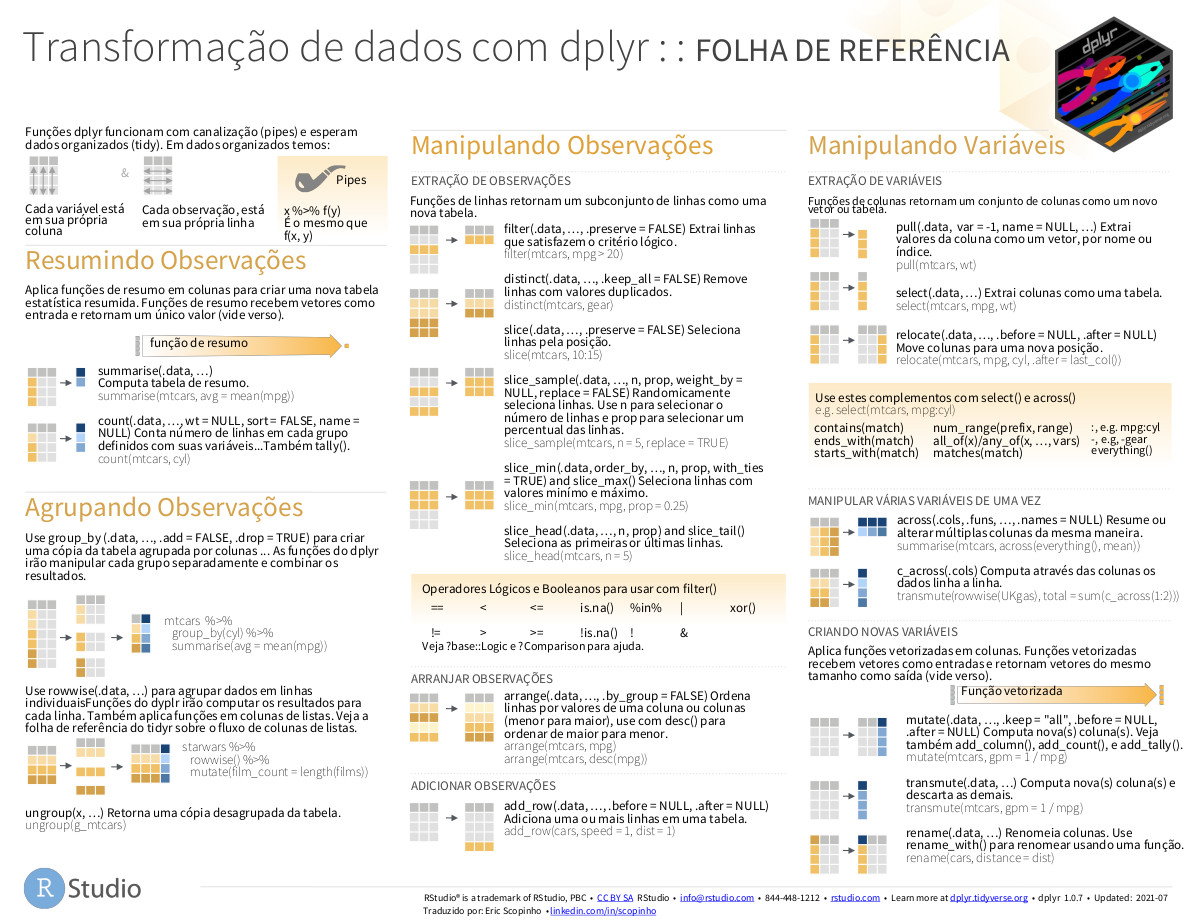
\includegraphics[width=6.90625in,height=\textheight]{./images/data-transformation-cheatsheet01.jpg}

Ao longo das apresentações das \textbf{Folhas de Resumo} e respectivos
capítulos sobre os pacotes, iremos lidar com nomenclaturas que são muito
comuns no âmbito da ciência de dados e estatística, mas podem não ser
comuns para outras áreas da ciência ou dos negócios, portanto, iremos
apresentar algumas delas brevemente para que você possa acompanhar de
forma mais clara os capítulos seguintes.

\hypertarget{variuxe1veis-e-observauxe7uxf5es}{%
\section*{Variáveis e
Observações}\label{variuxe1veis-e-observauxe7uxf5es}}
\addcontentsline{toc}{section}{Variáveis e Observações}

Apesar de comumente associarmos o termo \textbf{variável} à valores do
campo da matemática, como álgebra, ela também é usado em muitos outros
campos do conhecimento, como o da computação, estatística, etc.

Neste livro utilizaremos o termo ``\textbf{variável}'' no contexto de
ciência de dados e estatística. Iremos definí-la como uma característica
da população que pode ser categorizada, medida ou contada .

Sem entrarmos em maiores detalhes e simplificando para o melhor
entendimento deste conteúdo, pense em uma \textbf{tabela}, com
\textbf{colunas} e \textbf{linhas}. Em geral, quando temos dados
organizados (veremos o que caracteriza um dado organizado mais adiante),
as \textbf{variáveis são colocadas em colunas}. Já nas \textbf{linhas}
da tabela, teremos o que é conhecido como casos, ou
\textbf{observações}.

Apesar de não serem sinônimos, ou não representarem o mesmo objeto,
utilizaremos de forma intercambiável e sem o rigor acadêmico, os termos:
\textbf{coluna} e \textbf{variável} assim como \textbf{observações} e
\textbf{linhas}.

Portanto, quando em alguma parte do texto, você ler algo como
``\textbf{a variável xyz}'', pode traduzir em sua mente para algo como
``\textbf{a coluna xyz}''. Quando ler algo como ``\textbf{as 10
primeiras observações}'' , poder traduzir para ``\textbf{as 10 primeiras
linhas}'' e assim por diante.

Entendemos que desta forma, o leitor mais inciantes entenderá o conceito
daquilo que estamos apresentando, e o leitor mais avançado, o fará da
mesma forma.

\hypertarget{tipos-de-variuxe1veis}{%
\section*{Tipos de Variáveis}\label{tipos-de-variuxe1veis}}
\addcontentsline{toc}{section}{Tipos de Variáveis}

Como dito anteriormento, não é intuito deste tópico aprofundar neste
tema, porém como a natureza dos dados para manipulação e até mesmo cada
gráfico podem estar relacionadas ao \textbf{tipo de variável} que ele
irá representar, vamos rever de forma resumida os tipos de variáveis no
contexto de análise de dados.

Podemos categorizar as variáveis em \textbf{Qualitativas} ou
\textbf{Quantitativas}. (Fávero 2021)

\hypertarget{qualitativas}{%
\subsubsection*{Qualitativas}\label{qualitativas}}
\addcontentsline{toc}{subsubsection}{Qualitativas}

Representam as características de um indivíduo, objeto ou elemento que
não podem ser medidas ou quantificadas.

As variáveis \textbf{qualitativas}, também poder ser classificadas em
função do número de categorias em:

\begin{itemize}
\item
  \textbf{Dicotômica} ou \textbf{Binária}: Apenas duas categorias.
\item
  \textbf{Policotômica}: Mais que duas categorias.
\end{itemize}

Ou em função da escala de mensuração em:

\begin{itemize}
\item
  \textbf{Nominal}: As unidades são classificadas em categorias em
  relação à características representadas. Sem ordem ou relação entre
  si. (ex: sexo)
\item
  \textbf{Ordinal}: As unidades são classificadas em categorias em
  relação à características representadas. Há uma ordem ou relação entre
  si. (ex: grau de escolaridade)
\end{itemize}

Tipicamente, um dado qualitativo em natureza representa valores
discretos que pertencem a um conjunto finito de classes. Estes valores
discretos podem ser representados através de um número ou textos.

\hypertarget{quantitativa}{%
\subsubsection*{Quantitativa}\label{quantitativa}}
\addcontentsline{toc}{subsubsection}{Quantitativa}

Representam as características de um indivíduo, objeto ou elemento
resultantes de uma contagem ou mensuração.

As variáveis \textbf{quantitativas}, também podem ser classificadas em
função da escala de precisão.

\begin{itemize}
\item
  \textbf{Discreta}: Assumem conjunto finito de valores, frequentemente
  de uma contagem (ex: número de filhos, quantidade de carros, etc)
\item
  \textbf{Contínua}: Assumem conjunto infinito de valores,
  frequentemente com resultado de uma mensuração (ex: peso, altura,
  salário, etc)
\end{itemize}

Ou em função da escala de mensuração em:

\begin{itemize}
\item
  \textbf{Intervalar}: As unidades são ordenadas em relação à
  características mensurada e possui um unidade de constante. A origem,
  ou ponto zero, não expressa ausência de quantidade. (ex: temperatura)
\item
  \textbf{Razão}: As unidades são ordenadas em relação à características
  mensurada e possui um unidade de constante. A origem, ou ponto zero, é
  única e expressa ausência de quantidade.(ex: distância percorrida)
\end{itemize}

\begin{tcolorbox}[enhanced jigsaw, rightrule=.15mm, arc=.35mm, coltitle=black, colframe=quarto-callout-caution-color-frame, opacityback=0, toprule=.15mm, left=2mm, breakable, colback=white, bottomtitle=1mm, leftrule=.75mm, title=\textcolor{quarto-callout-caution-color}{\faFire}\hspace{0.5em}{Cuidado}, colbacktitle=quarto-callout-caution-color!10!white, titlerule=0mm, bottomrule=.15mm, toptitle=1mm, opacitybacktitle=0.6]
Vale lembrar que nem sempre uma variável representada por um número é
quantitativa. O número da carteira de identidade é um exemplo disso.
Apesar dos números ela é uma variável qualitativa.
\end{tcolorbox}

\hypertarget{exemplo}{%
\subsubsection*{Exemplo}\label{exemplo}}
\addcontentsline{toc}{subsubsection}{Exemplo}

Para ficar mais claro como estas classificações de variáveis serão
utilizadas ao longo do livro, vejamos alguns exemplos utilziando a
tabela chamada ``MPG'' abaixo:

\begin{Shaded}
\begin{Highlighting}[]
\NormalTok{mpg}
\end{Highlighting}
\end{Shaded}

\begin{verbatim}
# A tibble: 234 x 11
   manufacturer model      displ  year   cyl trans drv     cty   hwy fl    class
   <chr>        <chr>      <dbl> <int> <int> <chr> <chr> <int> <int> <chr> <chr>
 1 audi         a4           1.8  1999     4 auto~ f        18    29 p     comp~
 2 audi         a4           1.8  1999     4 manu~ f        21    29 p     comp~
 3 audi         a4           2    2008     4 manu~ f        20    31 p     comp~
 4 audi         a4           2    2008     4 auto~ f        21    30 p     comp~
 5 audi         a4           2.8  1999     6 auto~ f        16    26 p     comp~
 6 audi         a4           2.8  1999     6 manu~ f        18    26 p     comp~
 7 audi         a4           3.1  2008     6 auto~ f        18    27 p     comp~
 8 audi         a4 quattro   1.8  1999     4 manu~ 4        18    26 p     comp~
 9 audi         a4 quattro   1.8  1999     4 auto~ 4        16    25 p     comp~
10 audi         a4 quattro   2    2008     4 manu~ 4        20    28 p     comp~
# ... with 224 more rows
# i Use `print(n = ...)` to see more rows
\end{verbatim}

Esta tabela, possui dados de economia de combustíveis entre 1999 a 2008
de 38 modelos populares de carros.

Ela possui 234 observações (linhas) e 11 variáveis (colunas).

Vejamos algumas delas.

\begin{Shaded}
\begin{Highlighting}[]
\FunctionTok{glimpse}\NormalTok{(mpg)}
\end{Highlighting}
\end{Shaded}

\begin{verbatim}
Rows: 234
Columns: 11
$ manufacturer <chr> "audi", "audi", "audi", "audi", "audi", "audi", "audi", "~
$ model        <chr> "a4", "a4", "a4", "a4", "a4", "a4", "a4", "a4 quattro", "~
$ displ        <dbl> 1.8, 1.8, 2.0, 2.0, 2.8, 2.8, 3.1, 1.8, 1.8, 2.0, 2.0, 2.~
$ year         <int> 1999, 1999, 2008, 2008, 1999, 1999, 2008, 1999, 1999, 200~
$ cyl          <int> 4, 4, 4, 4, 6, 6, 6, 4, 4, 4, 4, 6, 6, 6, 6, 6, 6, 8, 8, ~
$ trans        <chr> "auto(l5)", "manual(m5)", "manual(m6)", "auto(av)", "auto~
$ drv          <chr> "f", "f", "f", "f", "f", "f", "f", "4", "4", "4", "4", "4~
$ cty          <int> 18, 21, 20, 21, 16, 18, 18, 18, 16, 20, 19, 15, 17, 17, 1~
$ hwy          <int> 29, 29, 31, 30, 26, 26, 27, 26, 25, 28, 27, 25, 25, 25, 2~
$ fl           <chr> "p", "p", "p", "p", "p", "p", "p", "p", "p", "p", "p", "p~
$ class        <chr> "compact", "compact", "compact", "compact", "compact", "c~
\end{verbatim}

Dentre as variáveis, observamos uma variável \textbf{qualitativa}
nominal chamada ``\textbf{manufacturer}'' que categoriza o fabricante do
veículo.

Já a variável ``hwy'', que representa o consumo na estrada (em milhas
por galão), pode ser categorizada como uma variavel
\textbf{quantitativa} continua. Por exemplo, determinado veículo
consegue fazer 25.73 milhas por galão.

\begin{tcolorbox}[enhanced jigsaw, rightrule=.15mm, arc=.35mm, coltitle=black, colframe=quarto-callout-note-color-frame, opacityback=0, toprule=.15mm, left=2mm, breakable, colback=white, bottomtitle=1mm, leftrule=.75mm, title=\textcolor{quarto-callout-note-color}{\faInfo}\hspace{0.5em}{Nota}, colbacktitle=quarto-callout-note-color!10!white, titlerule=0mm, bottomrule=.15mm, toptitle=1mm, opacitybacktitle=0.6]
No caso específico desta base de dados MPG, vemos que, a variável
``\textbf{hwy}'' está representada por um tipo inteiro
\textless int\textgreater, ao invés de um tipo double
\textless dbl\textgreater, isto nos leva a supor que ela foi
``\textbf{arredondada}'' para o valor mais próximo de milhas e portanto,
devemos classificá-la como \textbf{quantitativa} \textbf{discreta} para
sermos mais precisos.
\end{tcolorbox}

\hypertarget{dados-organizados-tidy}{%
\section*{Dados Organizados (Tidy)}\label{dados-organizados-tidy}}
\addcontentsline{toc}{section}{Dados Organizados (Tidy)}

Dados organizados (\emph{tidy}) são estruturados onde:

Cada \textbf{variável} está em sua própria \textbf{coluna} e cada
\textbf{observação} está em sua própria \textbf{linha}.

\includegraphics{././Organizacao/images/tidy_data01.png}

\hypertarget{canalizauxe7uxe3o-piping}{%
\section*{Canalização (Piping)}\label{canalizauxe7uxe3o-piping}}
\addcontentsline{toc}{section}{Canalização (Piping)}

A \textbf{canalização} (\emph{Piping}) é uma forma de sequenciar as
funções, facilitando a leitura de várias funções em conjunto.

O símbolo \textbf{\textbar\textgreater{}} é utilizado para esta
finalidade.

\textbf{Exemplo}: x \textbar\textgreater{} f(y), é o mesmo que f(x,y)

\begin{tcolorbox}[enhanced jigsaw, rightrule=.15mm, arc=.35mm, coltitle=black, colframe=quarto-callout-note-color-frame, opacityback=0, toprule=.15mm, left=2mm, breakable, colback=white, bottomtitle=1mm, leftrule=.75mm, title=\textcolor{quarto-callout-note-color}{\faInfo}\hspace{0.5em}{Nota}, colbacktitle=quarto-callout-note-color!10!white, titlerule=0mm, bottomrule=.15mm, toptitle=1mm, opacitybacktitle=0.6]
O símbolo \textbf{\%\textgreater\%} do pacote \textbf{magrittr} também
faz a função similar de pipe como o \textbar\textgreater{} do R básico,
porém com algumas vantagens. Como não precisamos utilizar nada além do
pipe básico, a maioria do código deste conteúdo utiliza o
\textbar\textgreater.
\end{tcolorbox}

Exemplo:

\begin{Shaded}
\begin{Highlighting}[]
\CommentTok{\# Escrever este código sem o Pipe (|\textgreater{})}
\FunctionTok{head}\NormalTok{(mtcars, }\DecValTok{5}\NormalTok{)}

\CommentTok{\#É o mesmo que escrever com o Pipe desta forma:}
\NormalTok{mtcars }\SpecialCharTok{|\textgreater{}} \FunctionTok{head}\NormalTok{(}\DecValTok{5}\NormalTok{)}
\end{Highlighting}
\end{Shaded}

No exemplo acima, pode não parecer muito vantajoso, mas quando nosso
código faz diversas manipulações, o uso da canalização (pipe) ajuda na
leitura e interpretação do código.

\hypertarget{vetores}{%
\section*{Vetores}\label{vetores}}
\addcontentsline{toc}{section}{Vetores}

Vetores é um tipo básico de objeto na linguagem R. Existem seis tipos de
vetores atômicos no R:

\begin{itemize}
\item
  lógicos (\emph{logical})
\item
  inteiros (\emph{integer})
\item
  duplos (\emph{doubles})
\item
  complexos (\emph{complex})
\item
  caractere (\emph{character})
\item
  bruto (\emph{raw})
\end{itemize}

Quando criamos apenas um valor, ele retorna um vetor de tamanho = 1.

Por exemplo:

\begin{Shaded}
\begin{Highlighting}[]
\CommentTok{\# Vetor atômico de caractere}
\FunctionTok{print}\NormalTok{(}\StringTok{"abc"}\NormalTok{)}
\end{Highlighting}
\end{Shaded}

\begin{verbatim}
[1] "abc"
\end{verbatim}

\begin{Shaded}
\begin{Highlighting}[]
\CommentTok{\# Vetor atômico de inteiro}
\FunctionTok{print}\NormalTok{(90L)}
\end{Highlighting}
\end{Shaded}

\begin{verbatim}
[1] 90
\end{verbatim}

\textbf{Vetore com múltiplos valores:}

Podemos criar vetores de múltiplos valores com algumas funções. Por
exemplo, para criar um vetor duplo em uma sequência númerica de 1.00 até
2.00, incrementando as cada 0.25, podemos usar a função \textbf{seq}():

\begin{Shaded}
\begin{Highlighting}[]
\FunctionTok{seq}\NormalTok{(}\FloatTok{1.00}\NormalTok{, }\FloatTok{2.00}\NormalTok{, }\AttributeTok{by =} \FloatTok{0.25}\NormalTok{)}
\end{Highlighting}
\end{Shaded}

\begin{verbatim}
[1] 1.00 1.25 1.50 1.75 2.00
\end{verbatim}

\begin{tcolorbox}[enhanced jigsaw, rightrule=.15mm, arc=.35mm, coltitle=black, colframe=quarto-callout-tip-color-frame, opacityback=0, toprule=.15mm, left=2mm, breakable, colback=white, bottomtitle=1mm, leftrule=.75mm, title=\textcolor{quarto-callout-tip-color}{\faLightbulb}\hspace{0.5em}{Dica}, colbacktitle=quarto-callout-tip-color!10!white, titlerule=0mm, bottomrule=.15mm, toptitle=1mm, opacitybacktitle=0.6]
Podemos utilizar dois-pontos (:) para criar uma vetor de múltiplos
valores númerico no R também:
\end{tcolorbox}

\begin{Shaded}
\begin{Highlighting}[]
\DecValTok{5}\SpecialCharTok{:}\DecValTok{10}
\end{Highlighting}
\end{Shaded}

\begin{verbatim}
[1]  5  6  7  8  9 10
\end{verbatim}

Para criarmos um vetor múltiplo, onde valores que não são do tipo
caractere são convertidos para caratectere, podemos usar a função
\textbf{c()}.

\begin{Shaded}
\begin{Highlighting}[]
\FunctionTok{c}\NormalTok{(}\DecValTok{5}\NormalTok{, }\ConstantTok{TRUE}\NormalTok{, }\StringTok{"banana"}\NormalTok{)}
\end{Highlighting}
\end{Shaded}

\begin{verbatim}
[1] "5"      "TRUE"   "banana"
\end{verbatim}

Veja que as aspas acima em ``5'' e ``TRUE'', definem um tipo caractere e
não mais inteiro ou lógico.

Para acessar elementos de um vetor, podemos usar colchetes e o
respectivo índice do elemento (começando em 1).

\begin{Shaded}
\begin{Highlighting}[]
\NormalTok{dia\_semana }\OtherTok{\textless{}{-}} \FunctionTok{c}\NormalTok{(}\StringTok{"Seg"}\NormalTok{, }\StringTok{"Ter"}\NormalTok{, }\StringTok{"Qua"}\NormalTok{, }\StringTok{"Qui"}\NormalTok{, }\StringTok{"Sex"}\NormalTok{, }\StringTok{"Sab"}\NormalTok{, }\StringTok{"Dom"}\NormalTok{)}
\NormalTok{dia\_semana\_num }\OtherTok{\textless{}{-}}\NormalTok{ dia\_semana[}\FunctionTok{c}\NormalTok{(}\DecValTok{1}\NormalTok{,}\DecValTok{2}\NormalTok{,}\DecValTok{5}\NormalTok{)]}

\NormalTok{dia\_semana\_num}
\end{Highlighting}
\end{Shaded}

\begin{verbatim}
[1] "Seg" "Ter" "Sex"
\end{verbatim}

Podemos acessar também passando um vetor lógico. Veja o exemplo:

\begin{Shaded}
\begin{Highlighting}[]
\NormalTok{dia\_semana[}\FunctionTok{c}\NormalTok{(}\ConstantTok{TRUE}\NormalTok{, }\ConstantTok{TRUE}\NormalTok{, }\ConstantTok{FALSE}\NormalTok{, }\ConstantTok{FALSE}\NormalTok{, }\ConstantTok{TRUE}\NormalTok{, }\ConstantTok{FALSE}\NormalTok{, }\ConstantTok{FALSE}\NormalTok{)]}
\end{Highlighting}
\end{Shaded}

\begin{verbatim}
[1] "Seg" "Ter" "Sex"
\end{verbatim}

Estas informações introdutórias farão mais sentido quando as utilzarmos
mais adiante nos capítulos seguintes. Por hora, basta conhecê-las para
entendê-las quando elas aparecerem nos códigos seguintes.

\part{Parte 1 - Obtendo e Manipulando os Dados}

\hypertarget{importauxe7uxe3o-de-dados-com-tidyverse}{%
\chapter{Importação de Dados com
TIDYVERSE}\label{importauxe7uxe3o-de-dados-com-tidyverse}}

\hypertarget{introduuxe7uxe3o-1}{%
\section{Introdução}\label{introduuxe7uxe3o-1}}

A seguir temos vários exemplos de importação de dados utilizando o
pacote TIDYVERSE do R. O pacote tidyverse possui vários pacotes de
importação de dados, aqui iremos cobrir três deles (readr, readxl e
googlesheets4). Para saber mais sobre estes pacotes, acesse:

\href{https://cran.r-project.org/package=tidyr}{https://cran.r-project.org/package=tidyverse}.

\url{https://cran.r-project.org/package=readr}.

\url{https://cran.r-project.org/package=readxl}.

\url{https://cran.r-project.org/package=googlesheets4}.

Os pacotes acima, serão utilzados para importação de dados tabulados
(ex: .CSV ou TXT), planilhas do Excel e do Google.

Caso você precise trabalhar com outras formatos de arquivos que não
sejam os vistos neste capítulo, pode buscar maiores informações sobre os
pacotes a seguir:

\begin{longtable}[]{@{}ll@{}}
\toprule()
Pacote & Formato \\
\midrule()
\endhead
haven & Arquivos SPSS, Stata e SAS \\
DBI & Bancos de Dados \\
jsonlite & JSON \\
xml2 & XML \\
httr & Web APIs \\
rvest & HTML (Web scraping) \\
readr::read\_lines() & dados texto \\
pdftools & PDF \\
\bottomrule()
\end{longtable}

Para os exemplos, iremos carregar os seguintes pacotes:

\begin{itemize}
\item
  \textbf{tidyverse}
\item
  \textbf{readxl}
\item
  \textbf{googlesheets4}
\item
  \textbf{openxlsx}
\end{itemize}

\begin{Shaded}
\begin{Highlighting}[]
\FunctionTok{library}\NormalTok{ (tidyverse)}
\FunctionTok{library}\NormalTok{ (readxl)}
\FunctionTok{library}\NormalTok{ (googlesheets4)}
\FunctionTok{library}\NormalTok{ (openxlsx)}
\end{Highlighting}
\end{Shaded}

\hypertarget{exemplos-da-folha-de-referuxeancia}{%
\subsection{Exemplos da Folha de
Referência}\label{exemplos-da-folha-de-referuxeancia}}

A maioria dos exemplos, visam ajudar na interpretação dos exemplos e
funções encontradas na
\href{https://github.com/scopinho/R-cheatsheets/blob/main/translations/portuguese/data-import_pt_br.pdf}{\textbf{Folha
de Referência}} de importação de dados com tidyverse disponível no site
do \href{rstudio.com}{RStudio}.

\begin{figure}

{\centering 

\href{images/cs-import-01.png}{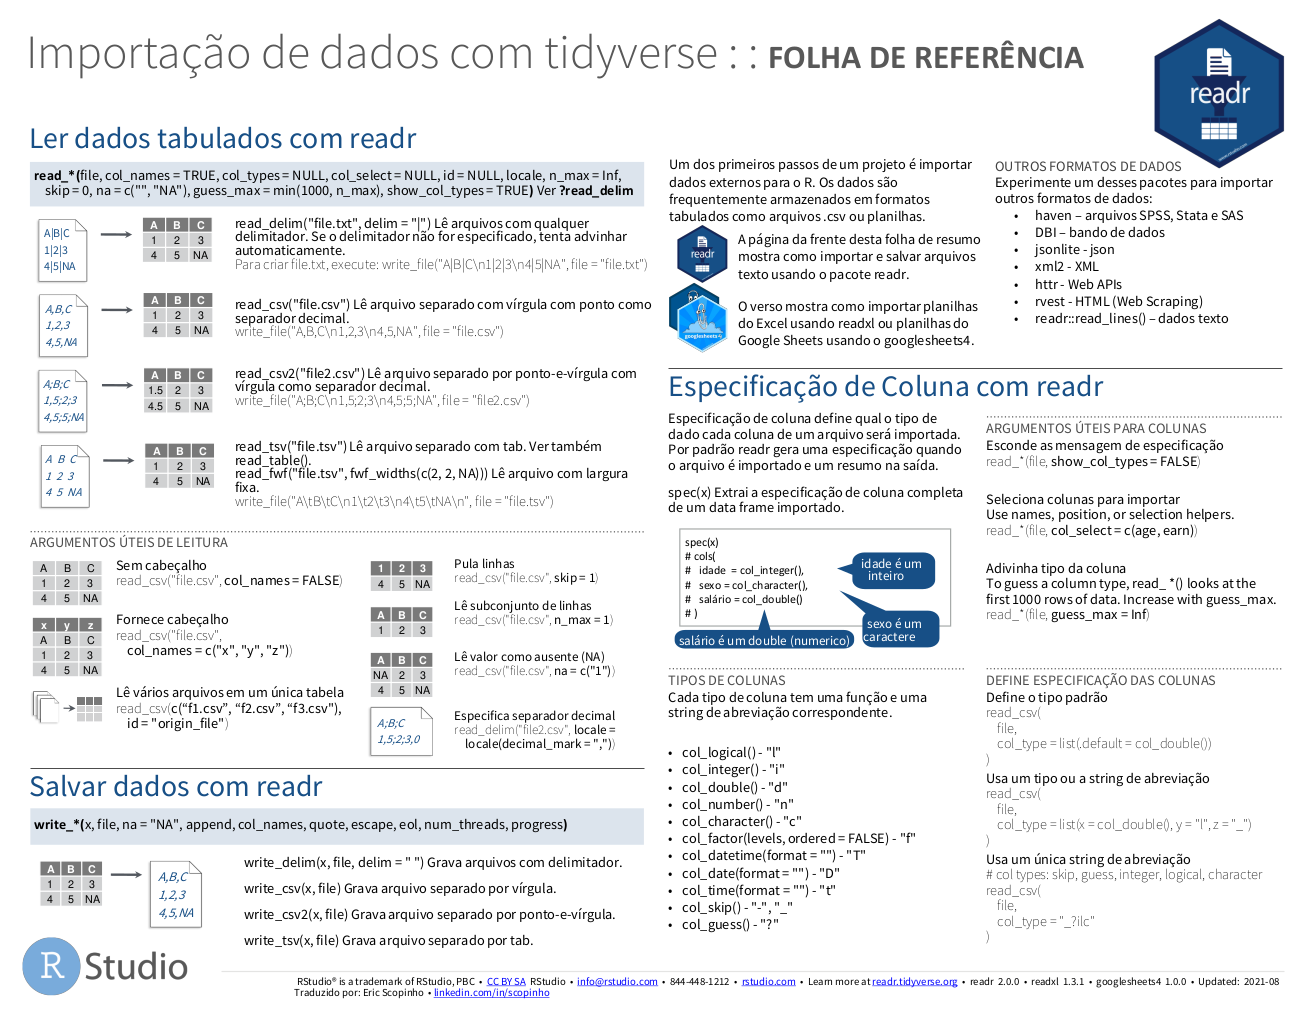
\includegraphics{Importacao/images/cs-import-01.png}}

}

\end{figure}

\begin{figure}

{\centering 

\href{images/cs-import-02.png}{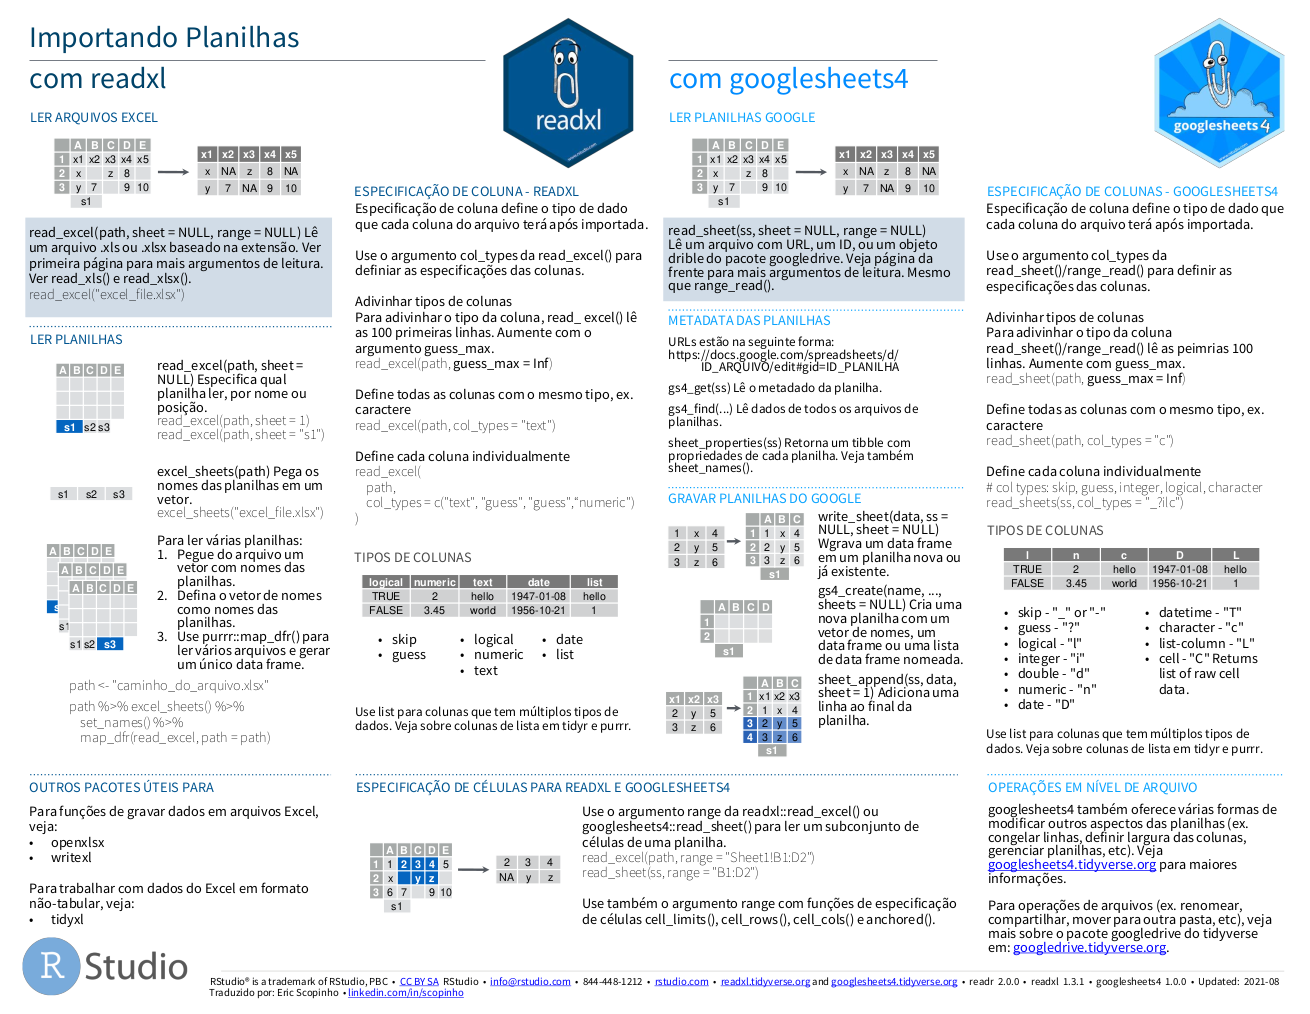
\includegraphics{Importacao/images/cs-import-02.png}}

}

\end{figure}

\hypertarget{arquivos}{%
\subsection{Arquivos}\label{arquivos}}

Para a maioria dos exemplos utilizaremos os seguintes arquivos de dados:

Alguns desses arquivos são baseados nas tabelas \textbf{mtcars, storms}
e \textbf{starwars} provenientes do pacote \textbf{datasets e dplyr e}
também algumas tabelas (\textbf{Table1}, \textbf{2, 3, 4a, 4b e 5}) que
vem com o pacote \textbf{tidyr}.

\begin{center}\rule{0.5\linewidth}{0.5pt}\end{center}

\textbf{ARQUIVOS TABULADOS: (TXT, CSV, TSV e FWF)}:

Iremos criar os arquivos tabulados para que possamos usá-los
posteriormente. Para isso, execute o código abaixo:

\begin{Shaded}
\begin{Highlighting}[]
\FunctionTok{write\_file}\NormalTok{(}\StringTok{"A|B|C}\SpecialCharTok{\textbackslash{}n}\StringTok{1|2|3}\SpecialCharTok{\textbackslash{}n}\StringTok{4|5|NA"}\NormalTok{, }\AttributeTok{file =} \StringTok{"file.txt"}\NormalTok{)}
\FunctionTok{write\_file}\NormalTok{(}\StringTok{"A,B,C}\SpecialCharTok{\textbackslash{}n}\StringTok{1,2,3}\SpecialCharTok{\textbackslash{}n}\StringTok{4,5,NA"}\NormalTok{, }\AttributeTok{file =} \StringTok{"file.csv"}\NormalTok{)}
\FunctionTok{write\_file}\NormalTok{(}\StringTok{"A;B;C}\SpecialCharTok{\textbackslash{}n}\StringTok{1,5;2;3}\SpecialCharTok{\textbackslash{}n}\StringTok{4,5;5;NA"}\NormalTok{, }\AttributeTok{file =} \StringTok{"file2.csv"}\NormalTok{)}
\FunctionTok{write\_file}\NormalTok{(}\StringTok{"A}\SpecialCharTok{\textbackslash{}t}\StringTok{B}\SpecialCharTok{\textbackslash{}t}\StringTok{C}\SpecialCharTok{\textbackslash{}n}\StringTok{1}\SpecialCharTok{\textbackslash{}t}\StringTok{2}\SpecialCharTok{\textbackslash{}t}\StringTok{3}\SpecialCharTok{\textbackslash{}n}\StringTok{4}\SpecialCharTok{\textbackslash{}t}\StringTok{5}\SpecialCharTok{\textbackslash{}t}\StringTok{NA}\SpecialCharTok{\textbackslash{}n}\StringTok{"}\NormalTok{, }\AttributeTok{file =} \StringTok{"file.tsv"}\NormalTok{)}
\end{Highlighting}
\end{Shaded}

\begin{center}\rule{0.5\linewidth}{0.5pt}\end{center}

\textbf{EXCEL\_FILE.XLSX}:

A seguir, você tem um link para o arquivo Excel utilizado nos exemplos.

\href{https://github.com/scopinho/Livro_Transform_Dados_R/blob/main/Importacao/excel_file.xlsx}{Arquivo
Exemplo - MS Excel}

É um arquivo com três planilhas (S1, S2 e S3) e em cada uma delas um
pequeno conjunto de dados.

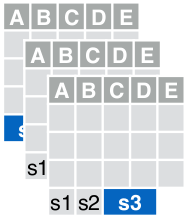
\includegraphics{Importacao/images/excel-workbooks.png}

E a primeira planilha (S1) possui algo como:

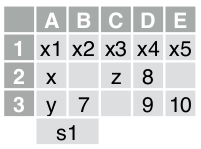
\includegraphics{Importacao/images/excel-worksheet.png}

\begin{center}\rule{0.5\linewidth}{0.5pt}\end{center}

\textbf{GOOGLE\_SHEET}:

A seguir, você tem o link para a planilha do google que será utilizado
mais adiante.

\href{https://docs.google.com/spreadsheets/d/1_aRR_9UcMytZqjID0BkJ7PW29M1kt1_x2HxhBZOlFN8/edit\#gid=0}{Planilha
exemplo - Google Sheets}

\begin{center}\rule{0.5\linewidth}{0.5pt}\end{center}

\hypertarget{readr}{%
\section{READR}\label{readr}}

O pacote readr possui diversas funções para ler dados tabulados (ex:
.csv, .tsv, .txt, etc). Estas funções começam com read\_*().

\textbf{read\_*} \emph{(file, col\_names = TRUE, col\_types = NULL,
col\_select = NULL, id = NULL, locale, n\_max = Inf, skip = 0, na =
c(````,''NA''), guess\_max = min(1000, n\_max), show\_col\_types =
TRUE)}

Os parametros acima, são comuns à estas funções. Veja a seguir algumas
delas. Digite \textbf{?read\_delim} para obter maiores detalhes de como
utilzá-las.

\hypertarget{ler-dados-tabulados-com-readr}{%
\subsection{Ler dados tabulados com
readr}\label{ler-dados-tabulados-com-readr}}

\hypertarget{read_delim}{%
\subsubsection{read\_delim}\label{read_delim}}

Use para ler um arquivo tabulado com qualquer delimitador. Se nenhum
delimitador é especificado, a função tentará advinhar automaticamente.

Por exemplo, para ler um arquivo .TXT tabulado com o caractere
``\textbar{}'' como delimitador, fazemos:

\begin{Shaded}
\begin{Highlighting}[]
\FunctionTok{read\_delim}\NormalTok{(}\StringTok{"file.txt"}\NormalTok{, }\AttributeTok{delim =} \StringTok{"|"}\NormalTok{) }
\end{Highlighting}
\end{Shaded}

\begin{verbatim}
# A tibble: 2 x 3
      A     B     C
  <dbl> <dbl> <dbl>
1     1     2     3
2     4     5    NA
\end{verbatim}

\begin{tcolorbox}[enhanced jigsaw, rightrule=.15mm, arc=.35mm, coltitle=black, colframe=quarto-callout-tip-color-frame, opacityback=0, toprule=.15mm, left=2mm, breakable, colback=white, bottomtitle=1mm, leftrule=.75mm, title=\textcolor{quarto-callout-tip-color}{\faLightbulb}\hspace{0.5em}{Dica}, colbacktitle=quarto-callout-tip-color!10!white, titlerule=0mm, bottomrule=.15mm, toptitle=1mm, opacitybacktitle=0.6]
Para armazenar a leitura do arquivo em um objeto no R, podemos usar o
operador \textless-.
\end{tcolorbox}

\begin{Shaded}
\begin{Highlighting}[]
\NormalTok{meu\_arquivo\_csv }\OtherTok{\textless{}{-}}\FunctionTok{read\_delim}\NormalTok{(}\StringTok{"file.txt"}\NormalTok{, }\AttributeTok{delim =} \StringTok{"|"}\NormalTok{)}
\NormalTok{meu\_arquivo\_csv}
\end{Highlighting}
\end{Shaded}

\begin{verbatim}
# A tibble: 2 x 3
      A     B     C
  <dbl> <dbl> <dbl>
1     1     2     3
2     4     5    NA
\end{verbatim}

\hypertarget{read_cvs}{%
\subsubsection{read\_cvs}\label{read_cvs}}

Use para ler um arquivo tabulado \textbf{separado por vírgula}. Esta
função entende que casas decimais que usam o \textbf{ponto} (ex 1.00)
como separador de \textbf{casas decimais}.

\begin{Shaded}
\begin{Highlighting}[]
\FunctionTok{read\_csv}\NormalTok{(}\StringTok{"file.csv"}\NormalTok{) }
\end{Highlighting}
\end{Shaded}

\begin{verbatim}
# A tibble: 2 x 3
      A     B     C
  <dbl> <dbl> <dbl>
1     1     2     3
2     4     5    NA
\end{verbatim}

\hypertarget{read_cvs2}{%
\subsubsection{read\_cvs2}\label{read_cvs2}}

Use para ler um arquivo tabulado \textbf{separado por ponto-e-vírgula}.
Esta função entende que casas decimais que usam a \textbf{vírgula} (ex:
1,00) como separador de \textbf{casas decimais}.

\begin{Shaded}
\begin{Highlighting}[]
\FunctionTok{read\_csv2}\NormalTok{(}\StringTok{"file2.csv"}\NormalTok{) }
\end{Highlighting}
\end{Shaded}

\begin{verbatim}
# A tibble: 2 x 3
      A     B     C
  <dbl> <dbl> <dbl>
1   1.5     2     3
2   4.5     5    NA
\end{verbatim}

\hypertarget{read_tsv}{%
\subsubsection{read\_tsv}\label{read_tsv}}

Use para ler um arquivo tabulado \textbf{separado por tab}.

\begin{Shaded}
\begin{Highlighting}[]
\FunctionTok{read\_tsv}\NormalTok{(}\StringTok{"file.tsv"}\NormalTok{) }
\end{Highlighting}
\end{Shaded}

\begin{verbatim}
# A tibble: 2 x 3
      A     B     C
  <dbl> <dbl> <dbl>
1     1     2     3
2     4     5    NA
\end{verbatim}

\hypertarget{read_fwf}{%
\subsubsection{read\_fwf}\label{read_fwf}}

Use para ler um arquivo tabulado \textbf{com tamanhos fixos de colunas}.

\begin{tcolorbox}[enhanced jigsaw, rightrule=.15mm, arc=.35mm, coltitle=black, colframe=quarto-callout-note-color-frame, opacityback=0, toprule=.15mm, left=2mm, breakable, colback=white, bottomtitle=1mm, leftrule=.75mm, title=\textcolor{quarto-callout-note-color}{\faInfo}\hspace{0.5em}{Nota}, colbacktitle=quarto-callout-note-color!10!white, titlerule=0mm, bottomrule=.15mm, toptitle=1mm, opacitybacktitle=0.6]
Veja que a largura das colunas deve ser passada como um vetor para a
parametro col\_positions = usando a função fwf\_width().
\end{tcolorbox}

\begin{Shaded}
\begin{Highlighting}[]
\FunctionTok{read\_fwf}\NormalTok{(}\StringTok{"file.tsv"}\NormalTok{, }\FunctionTok{fwf\_widths}\NormalTok{(}\FunctionTok{c}\NormalTok{(}\DecValTok{2}\NormalTok{,}\DecValTok{2}\NormalTok{,}\ConstantTok{NA}\NormalTok{)))}
\end{Highlighting}
\end{Shaded}

\begin{verbatim}
# A tibble: 3 x 3
  X1    X2    X3   
  <chr> <chr> <chr>
1 A     B     C    
2 1     2     3    
3 4     5     <NA> 
\end{verbatim}

\hypertarget{paruxe2metros-uxfateis}{%
\subsection{Parâmetros Úteis}\label{paruxe2metros-uxfateis}}

Alguns parametros das funções read\_*() são muito úteis durante o
processo de leitura pois permitem controlar melhor o que iremos obter
como resultado da leitura.

\hypertarget{sem-cabeuxe7alho}{%
\subsubsection{Sem cabeçalho}\label{sem-cabeuxe7alho}}

Use o parâmetro \textbf{COL\_NAMES} para não trazer a primeira linha
como nome das colunas.

\begin{Shaded}
\begin{Highlighting}[]
\FunctionTok{read\_csv2}\NormalTok{(}\StringTok{"file2.csv"}\NormalTok{, }\AttributeTok{col\_names =} \ConstantTok{FALSE}\NormalTok{) }
\end{Highlighting}
\end{Shaded}

\begin{verbatim}
# A tibble: 3 x 3
  X1    X2    X3   
  <chr> <chr> <chr>
1 A     B     C    
2 1,5   2     3    
3 4,5   5     <NA> 
\end{verbatim}

\hypertarget{definir-cabeuxe7alho}{%
\subsubsection{Definir cabeçalho}\label{definir-cabeuxe7alho}}

Use o parâmetro \textbf{COL\_NAMES} para definir manualmente os nomes
das colunas.

\begin{Shaded}
\begin{Highlighting}[]
\FunctionTok{read\_csv}\NormalTok{(}\StringTok{"file.csv"}\NormalTok{, }\AttributeTok{col\_names =} \FunctionTok{c}\NormalTok{(}\StringTok{"X"}\NormalTok{, }\StringTok{"Y"}\NormalTok{, }\StringTok{"Z"}\NormalTok{)) }
\end{Highlighting}
\end{Shaded}

\begin{verbatim}
# A tibble: 3 x 3
  X     Y     Z    
  <chr> <chr> <chr>
1 A     B     C    
2 1     2     3    
3 4     5     <NA> 
\end{verbatim}

\hypertarget{ler-vuxe1rios-arquivos}{%
\subsubsection{Ler vários arquivos}\label{ler-vuxe1rios-arquivos}}

Use o parametro \textbf{ID} para ler multiplos arquivos e armazená-los
em uma mesma tabela.

\begin{Shaded}
\begin{Highlighting}[]
\FunctionTok{write\_file}\NormalTok{(}\StringTok{"A,B,C}\SpecialCharTok{\textbackslash{}n}\StringTok{1,2,3}\SpecialCharTok{\textbackslash{}n}\StringTok{4,5,NA"}\NormalTok{, }\AttributeTok{file =} \StringTok{"f1.csv"}\NormalTok{)}
\FunctionTok{write\_file}\NormalTok{(}\StringTok{"A,B,C}\SpecialCharTok{\textbackslash{}n}\StringTok{6,7,8}\SpecialCharTok{\textbackslash{}n}\StringTok{9,10,11"}\NormalTok{, }\AttributeTok{file =} \StringTok{"f2.csv"}\NormalTok{)}
\FunctionTok{read\_csv}\NormalTok{(}\FunctionTok{c}\NormalTok{(}\StringTok{"f1.csv"}\NormalTok{, }\StringTok{"f2.csv"}\NormalTok{), }\AttributeTok{id =} \StringTok{"arq\_origem"}\NormalTok{) }
\end{Highlighting}
\end{Shaded}

\begin{verbatim}
# A tibble: 4 x 4
  arq_origem     A     B     C
  <chr>      <dbl> <dbl> <dbl>
1 f1.csv         1     2     3
2 f1.csv         4     5    NA
3 f2.csv         6     7     8
4 f2.csv         9    10    11
\end{verbatim}

\begin{tcolorbox}[enhanced jigsaw, rightrule=.15mm, arc=.35mm, coltitle=black, colframe=quarto-callout-important-color-frame, opacityback=0, toprule=.15mm, left=2mm, breakable, colback=white, bottomtitle=1mm, leftrule=.75mm, title=\textcolor{quarto-callout-important-color}{\faExclamation}\hspace{0.5em}{Importante}, colbacktitle=quarto-callout-important-color!10!white, titlerule=0mm, bottomrule=.15mm, toptitle=1mm, opacitybacktitle=0.6]
Observe que as colunas dos diversos arquivos devem corresponder, ou
seja, ter o mesmo nome de colunas.
\end{tcolorbox}

\hypertarget{pular-linhas}{%
\subsubsection{Pular linhas}\label{pular-linhas}}

Use o prâmetro SKIP para pular as primeiras n linhas.

\begin{Shaded}
\begin{Highlighting}[]
\FunctionTok{read\_csv}\NormalTok{(}\StringTok{"file.csv"}\NormalTok{, }\AttributeTok{skip =} \DecValTok{1}\NormalTok{) }
\end{Highlighting}
\end{Shaded}

\begin{verbatim}
# A tibble: 1 x 3
    `1`   `2` `3`  
  <dbl> <dbl> <lgl>
1     4     5 NA   
\end{verbatim}

\hypertarget{ler-um-nuxfamero-muxe1ximo-de-linhas}{%
\subsubsection{Ler um número máximo de
linhas}\label{ler-um-nuxfamero-muxe1ximo-de-linhas}}

Use o prâmetro \textbf{N\_MAX} para ler um número máximo de linhas.

\begin{Shaded}
\begin{Highlighting}[]
\FunctionTok{read\_csv}\NormalTok{(}\StringTok{"file.csv"}\NormalTok{, }\AttributeTok{n\_max =} \DecValTok{1}\NormalTok{) }
\end{Highlighting}
\end{Shaded}

\begin{verbatim}
# A tibble: 1 x 3
      A     B     C
  <dbl> <dbl> <dbl>
1     1     2     3
\end{verbatim}

\hypertarget{ler-valores-como-na}{%
\subsubsection{Ler valores como NA}\label{ler-valores-como-na}}

Use o prâmetro \textbf{NA} para definir um ou mais valores como NA.

\begin{Shaded}
\begin{Highlighting}[]
\FunctionTok{read\_csv}\NormalTok{(}\StringTok{"file.csv"}\NormalTok{, }\AttributeTok{na =} \FunctionTok{c}\NormalTok{(}\StringTok{"1"}\NormalTok{)) }
\end{Highlighting}
\end{Shaded}

\begin{verbatim}
# A tibble: 2 x 3
      A     B C    
  <dbl> <dbl> <chr>
1    NA     2 3    
2     4     5 NA   
\end{verbatim}

\hypertarget{especificar-caractere-decimal}{%
\subsubsection{Especificar caractere
decimal}\label{especificar-caractere-decimal}}

Use o prâmetro \textbf{LOCALE} para definir o caractere de casa
decimais.

\begin{Shaded}
\begin{Highlighting}[]
\FunctionTok{read\_delim}\NormalTok{(}\StringTok{"file2.csv"}\NormalTok{, }\AttributeTok{locale =} \FunctionTok{locale}\NormalTok{(}\AttributeTok{decimal\_mark =} \StringTok{","}\NormalTok{)) }
\end{Highlighting}
\end{Shaded}

\begin{verbatim}
# A tibble: 2 x 3
      A     B     C
  <dbl> <dbl> <dbl>
1   1.5     2     3
2   4.5     5    NA
\end{verbatim}

\hypertarget{salvar-dados-com-readr}{%
\subsection{Salvar dados com readr}\label{salvar-dados-com-readr}}

Similar às funções descritas na seção
``\protect\hyperlink{ler-dados-tabulados-com-readr}{Ler dados tabulados
com readr}'' usadas para ler os aqruivos de texto tabulados, temos o
conjunto de funções \textbf{write\_*}() para gravar os arquivos
correspondentes. Estas funções seguem o seguinte padrão:

write\_*(x, file, na = ``NA'', append, col\_names, quote, escape, eol,
num\_threads, progress)

As principais funções são:

\hypertarget{write_delim}{%
\subsubsection{write\_delim}\label{write_delim}}

Use para gravar um arquivo delimitado por algum caractere específico. O
parametro delim= permite definir este caractere. O caracteres padrão é o
espaço ('' ``).

Por exemplo, se quisermos gravar uma tabela (tibble) em um arquivo .txt
delimitado por ponto-e-vírgula'';``, podemos usar:

\begin{Shaded}
\begin{Highlighting}[]
\NormalTok{conteudo }\OtherTok{\textless{}{-}} \FunctionTok{tribble}\NormalTok{(}\SpecialCharTok{\textasciitilde{}}\NormalTok{col\_A, }\SpecialCharTok{\textasciitilde{}}\NormalTok{col\_B,}
                   \DecValTok{1}\NormalTok{, }\StringTok{"A"}\NormalTok{,}
                   \DecValTok{2}\NormalTok{, }\StringTok{"B"}\NormalTok{, }
                   \DecValTok{3}\NormalTok{, }\StringTok{"C"}\NormalTok{)}
\FunctionTok{write\_delim}\NormalTok{(conteudo, }\AttributeTok{file =} \StringTok{"arquivo\_exemplo1.txt"}\NormalTok{, }\AttributeTok{delim=}\StringTok{";"}\NormalTok{)}
\end{Highlighting}
\end{Shaded}

\hypertarget{write_csv}{%
\subsubsection{write\_csv}\label{write_csv}}

Use para gravar uma tabela em uma arquivo delimitado por ``vírgula''.

\begin{tcolorbox}[enhanced jigsaw, rightrule=.15mm, arc=.35mm, coltitle=black, colframe=quarto-callout-tip-color-frame, opacityback=0, toprule=.15mm, left=2mm, breakable, colback=white, bottomtitle=1mm, leftrule=.75mm, title=\textcolor{quarto-callout-tip-color}{\faLightbulb}\hspace{0.5em}{Dica}, colbacktitle=quarto-callout-tip-color!10!white, titlerule=0mm, bottomrule=.15mm, toptitle=1mm, opacitybacktitle=0.6]
Podemos usar o arqumento \textbf{na =} para definirmos qual valor será
usando para os valore ausentes, por padrão é utilizado ``NA''. No
exemplo a seguir, iremos trocar por ``NULL''.
\end{tcolorbox}

\begin{Shaded}
\begin{Highlighting}[]
\NormalTok{conteudo }\OtherTok{\textless{}{-}} \FunctionTok{tribble}\NormalTok{(}\SpecialCharTok{\textasciitilde{}}\NormalTok{col\_A, }\SpecialCharTok{\textasciitilde{}}\NormalTok{col\_B,}
                   \DecValTok{1}\NormalTok{, }\StringTok{"A"}\NormalTok{,}
                   \DecValTok{2}\NormalTok{, }\StringTok{"B"}\NormalTok{, }
                   \DecValTok{3}\NormalTok{, }\ConstantTok{NA}\NormalTok{,}
                   \DecValTok{4}\NormalTok{, }\StringTok{"D"}\NormalTok{)}
\FunctionTok{write\_csv}\NormalTok{(conteudo, }\AttributeTok{file =} \StringTok{"arquivo\_exemplo2.csv"}\NormalTok{, }\AttributeTok{na =} \StringTok{"NULL"}\NormalTok{)}
\end{Highlighting}
\end{Shaded}

\hypertarget{write_csv2}{%
\subsubsection{write\_csv2}\label{write_csv2}}

Use para gravar uma tabela em um arquivo delimitado por
``ponto-e-vírgula''.

\begin{tcolorbox}[enhanced jigsaw, rightrule=.15mm, arc=.35mm, coltitle=black, colframe=quarto-callout-tip-color-frame, opacityback=0, toprule=.15mm, left=2mm, breakable, colback=white, bottomtitle=1mm, leftrule=.75mm, title=\textcolor{quarto-callout-tip-color}{\faLightbulb}\hspace{0.5em}{Dica}, colbacktitle=quarto-callout-tip-color!10!white, titlerule=0mm, bottomrule=.15mm, toptitle=1mm, opacitybacktitle=0.6]
Pode usar o parametro ``\textbf{col\_names =}'' para incluir ou não os
nomes das colunas no arquivo de saída. No exemplo a seguir, não iremos
incluir os nomes das colunas:
\end{tcolorbox}

\begin{Shaded}
\begin{Highlighting}[]
\NormalTok{conteudo }\OtherTok{\textless{}{-}} \FunctionTok{tribble}\NormalTok{(}\SpecialCharTok{\textasciitilde{}}\NormalTok{col\_A, }\SpecialCharTok{\textasciitilde{}}\NormalTok{col\_B,}
                   \DecValTok{1}\NormalTok{, }\StringTok{"A"}\NormalTok{,}
                   \DecValTok{2}\NormalTok{, }\StringTok{"B"}\NormalTok{, }
                   \DecValTok{3}\NormalTok{, }\StringTok{"C"}\NormalTok{)}
\FunctionTok{write\_csv2}\NormalTok{(conteudo, }\AttributeTok{file =} \StringTok{"arquivo\_exemplo3.csv"}\NormalTok{, }\AttributeTok{col\_names =} \ConstantTok{FALSE}\NormalTok{)}
\end{Highlighting}
\end{Shaded}

\hypertarget{write_tsv}{%
\subsubsection{write\_tsv}\label{write_tsv}}

Use para gravar uma tabela em um arquivo delimitado por ``TAB'':

\begin{Shaded}
\begin{Highlighting}[]
\NormalTok{conteudo }\OtherTok{\textless{}{-}} \FunctionTok{tribble}\NormalTok{(}\SpecialCharTok{\textasciitilde{}}\NormalTok{col\_A, }\SpecialCharTok{\textasciitilde{}}\NormalTok{col\_B,}
                   \DecValTok{1}\NormalTok{, }\StringTok{"A"}\NormalTok{,}
                   \DecValTok{2}\NormalTok{, }\StringTok{"B"}\NormalTok{, }
                   \DecValTok{3}\NormalTok{, }\StringTok{"C"}\NormalTok{)}
\FunctionTok{write\_tsv}\NormalTok{(conteudo, }\AttributeTok{file =} \StringTok{"arquivo\_exemplo4.tsv"}\NormalTok{)}
\end{Highlighting}
\end{Shaded}

\hypertarget{especificauxe7uxe3o-de-colunas-com-readr}{%
\subsection{Especificação de colunas com
readr}\label{especificauxe7uxe3o-de-colunas-com-readr}}

Ao importar um arquivo com readr, podemos definir qual o tipo de coluna
que determinado dado será importado. Por padrão, o readr irá gerar a
especificação de cada coluna quando o arquivo form lido e gerará um
resumo na saída.

Podemos usar o argumento \textbf{spec()} para extrair as especificações
das colunas de um arquivo importato para um data frame.

Por exemplo:

\begin{Shaded}
\begin{Highlighting}[]
\NormalTok{arq }\OtherTok{\textless{}{-}} \FunctionTok{read\_csv2}\NormalTok{(}\StringTok{"file2.csv"}\NormalTok{) }
\FunctionTok{spec}\NormalTok{(arq)}
\end{Highlighting}
\end{Shaded}

\begin{verbatim}
cols(
  A = col_double(),
  B = col_double(),
  C = col_double()
)
\end{verbatim}

Observe que as colunas ``A'', ``B'' e ``C'' são do formato
\textbf{double}.

Há também uma mensagem de resumo ao importar um arquivo. Observe que ele
informa o delimitador utilzado, mas também a especificação das colunas,
neste caso, tipo double (\textbf{dbl}) para as colunas \textbf{A},
\textbf{B} e \textbf{C} conforme confirmamos com a função
\textbf{spec()}.

\begin{center}\rule{0.5\linewidth}{0.5pt}\end{center}

\emph{ℹ Using ``\,`,'\,'' as decimal and ``\,`.'\,'' as grouping mark.
Use \texttt{read\_delim()} for more control. Rows: 2 Columns: 3── Column
specification
──────────────────────────────────────────────────────────────────
Delimiter: ``;'' dbl (3): A, B, C ℹ Use \texttt{spec()} to retrieve the
full column specification for this data. ℹ Specify the column types or
set \texttt{show\_col\_types\ =\ FALSE} to quiet this message. \#
READXL}

\begin{center}\rule{0.5\linewidth}{0.5pt}\end{center}

\begin{tcolorbox}[enhanced jigsaw, rightrule=.15mm, arc=.35mm, coltitle=black, colframe=quarto-callout-tip-color-frame, opacityback=0, toprule=.15mm, left=2mm, breakable, colback=white, bottomtitle=1mm, leftrule=.75mm, title=\textcolor{quarto-callout-tip-color}{\faLightbulb}\hspace{0.5em}{Dica}, colbacktitle=quarto-callout-tip-color!10!white, titlerule=0mm, bottomrule=.15mm, toptitle=1mm, opacitybacktitle=0.6]
Se quisermos omitir as especificações das colunas da mensagem de saída,
usamos o parametro \textbf{show\_col\_types} = FALSE
\end{tcolorbox}

\hypertarget{col_types}{%
\subsubsection{\texorpdfstring{\textbf{col\_types}}{col\_types}}\label{col_types}}

Se utilizarmos o parametro \textbf{col\_types =} podemos definir, por
exemplo, a coluna ``B'' como inteiro (integer). Veja:

\begin{Shaded}
\begin{Highlighting}[]
\NormalTok{arq }\OtherTok{\textless{}{-}} \FunctionTok{read\_csv2}\NormalTok{(}\StringTok{"file2.csv"}\NormalTok{, }\AttributeTok{col\_types =} \StringTok{"did"}\NormalTok{) }
\FunctionTok{spec}\NormalTok{(arq)}
\end{Highlighting}
\end{Shaded}

\begin{verbatim}
cols(
  A = col_double(),
  B = col_integer(),
  C = col_double()
)
\end{verbatim}

Há uma letra definida para cada tipo de coluna que quisermos
especificar, veja a lista abaixo:

\emph{• col\_logical() - ``l''}

\emph{• col\_integer() - ``i''}

\emph{• col\_double() - ``d''}

\emph{• col\_number() - ``n''}

\emph{• col\_character() - ``c''}

\emph{• col\_factor(levels, ordered = FALSE) - ``f''}

\emph{• col\_datetime(format = ````) -''T''}

\emph{• col\_date(format = ````) -''D''}

\emph{• col\_time(format = ````) -''t''}

\emph{• col\_skip() - ``-'', ``\_''}

\emph{• col\_guess() - ``?''}

Por isso, usamos string \textbf{``did''} para definir um
\textbf{double}, um \textbf{inteiro} e outro \textbf{double} para as
colunas que importamos.

Podemos também passar a especificação das colunas como uma lista
mesclando as funções e os caracteres correspondentes na lista acima.

Por exemplo:

\begin{Shaded}
\begin{Highlighting}[]
\NormalTok{arq }\OtherTok{\textless{}{-}} \FunctionTok{read\_csv2}\NormalTok{(}\StringTok{"file2.csv"}\NormalTok{, }
          \AttributeTok{col\_types =} \FunctionTok{list}\NormalTok{(}\AttributeTok{A =} \FunctionTok{col\_double}\NormalTok{(), }\AttributeTok{B =} \StringTok{"i"}\NormalTok{, }\AttributeTok{C=} \StringTok{"d"}\NormalTok{)}
\NormalTok{          )}
\FunctionTok{spec}\NormalTok{(arq)}
\end{Highlighting}
\end{Shaded}

\begin{verbatim}
cols(
  A = col_double(),
  B = col_integer(),
  C = col_double()
)
\end{verbatim}

\begin{tcolorbox}[enhanced jigsaw, rightrule=.15mm, arc=.35mm, coltitle=black, colframe=quarto-callout-tip-color-frame, opacityback=0, toprule=.15mm, left=2mm, breakable, colback=white, bottomtitle=1mm, leftrule=.75mm, title=\textcolor{quarto-callout-tip-color}{\faLightbulb}\hspace{0.5em}{Dica}, colbacktitle=quarto-callout-tip-color!10!white, titlerule=0mm, bottomrule=.15mm, toptitle=1mm, opacitybacktitle=0.6]
Use ``\textbf{.default =}'' na lista de especificações para definir o
tipo padrão para as colunas, caso as mesmas não sejam explicitamente
definidas.
\end{tcolorbox}

\hypertarget{col_select}{%
\subsubsection{col\_select}\label{col_select}}

Para selecionarmos apenas algumas colunas para importar do arquivo,
utilzamos o parametro \textbf{col\_select} = passanto um vetor com o
nomes das colunas.

Por exemplo, para importar apenas as colunas ``A'' e ``C'', podemos
fazer:

\begin{Shaded}
\begin{Highlighting}[]
\FunctionTok{read\_csv}\NormalTok{(}\StringTok{"file.csv"}\NormalTok{, }\AttributeTok{col\_select =} \FunctionTok{c}\NormalTok{(}\StringTok{"A"}\NormalTok{, }\StringTok{"C"}\NormalTok{))}
\end{Highlighting}
\end{Shaded}

\begin{verbatim}
# A tibble: 2 x 2
      A     C
  <dbl> <dbl>
1     1     3
2     4    NA
\end{verbatim}

\hypertarget{guess_max}{%
\subsubsection{guess\_max}\label{guess_max}}

Para definirmos o número máximo de linhas do arquivo para advinhar o
tipo da coluna (guess), utilizamos o parametro \textbf{guess\_max} =. O
padrão são as primeiras 1000 linhas.

\begin{Shaded}
\begin{Highlighting}[]
\FunctionTok{read\_csv}\NormalTok{(}\StringTok{"file.csv"}\NormalTok{,}\AttributeTok{guess\_max =} \DecValTok{2}\NormalTok{)}
\end{Highlighting}
\end{Shaded}

\begin{verbatim}
# A tibble: 2 x 3
      A     B     C
  <dbl> <dbl> <dbl>
1     1     2     3
2     4     5    NA
\end{verbatim}

\hypertarget{readxl}{%
\section{READXL}\label{readxl}}

Para lermos arquivos do Microsoft Excel, podemos usar o pacote
\textbf{readxl}.

\hypertarget{ler-arquivos-do-excel}{%
\subsection{Ler arquivos do Excel}\label{ler-arquivos-do-excel}}

Apesar do pacote readxl ser instalado quando instalamos o pacote
tidyverse, ele não é carregado quando carregamos o tidyverse. É por
isso, que tivemos o código ``library (readxl) na seção
\protect\hyperlink{introduuxe7uxe3o-13}{Introdução}

\hypertarget{read_excel}{%
\subsubsection{read\_excel}\label{read_excel}}

Use para ler um arquivo do Excel (.xls ou .xlsx) baseado na extensão do
arquivo.

Se preferir, pode utilizar as funções read\_xls() e read\_xlsx() para
ler um arquivo com .xls ou .xlsx independente da extensão do arquivo.

\begin{Shaded}
\begin{Highlighting}[]
\FunctionTok{read\_excel}\NormalTok{(}\StringTok{"excel\_file.xlsx"}\NormalTok{)}
\end{Highlighting}
\end{Shaded}

\begin{verbatim}
# A tibble: 2 x 5
  x1       x2 x3       x4    x5
  <chr> <dbl> <chr> <dbl> <dbl>
1 x        NA z         8    NA
2 y         7 <NA>      9    10
\end{verbatim}

\hypertarget{ler-planilhas}{%
\subsection{Ler planilhas}\label{ler-planilhas}}

Sabemos que um arquivo Excel (\emph{workbook}), pode conter uma ou mais
planilhas (\emph{worksheets}). Para definirmos as planilhas que
precisamos importar, podemos utilizar o parametros \textbf{sheet =} da
função read\_excel(). Podemos passar uma string com o nome a planilha
(ex: ``S1'') ou um índice númerico pela ordem de criação da planilha
(ex: 1). Se nada for especificado, padrão é trazer a primeira planilha.

\begin{Shaded}
\begin{Highlighting}[]
\FunctionTok{read\_excel}\NormalTok{(}\StringTok{"excel\_file.xlsx"}\NormalTok{, }\AttributeTok{sheet =} \StringTok{"S1"}\NormalTok{)}
\end{Highlighting}
\end{Shaded}

\begin{verbatim}
# A tibble: 2 x 5
  x1       x2 x3       x4    x5
  <chr> <dbl> <chr> <dbl> <dbl>
1 x        NA z         8    NA
2 y         7 <NA>      9    10
\end{verbatim}

Para obter os nomes das planilhas presentes no arquivo, utilizamos a
função \textbf{excel\_sheets}()

\begin{Shaded}
\begin{Highlighting}[]
\FunctionTok{excel\_sheets}\NormalTok{(}\StringTok{"excel\_file.xlsx"}\NormalTok{)}
\end{Highlighting}
\end{Shaded}

\begin{verbatim}
[1] "S1" "S2" "S3"
\end{verbatim}

\begin{tcolorbox}[enhanced jigsaw, rightrule=.15mm, arc=.35mm, coltitle=black, colframe=quarto-callout-tip-color-frame, opacityback=0, toprule=.15mm, left=2mm, breakable, colback=white, bottomtitle=1mm, leftrule=.75mm, title=\textcolor{quarto-callout-tip-color}{\faLightbulb}\hspace{0.5em}{Dica}, colbacktitle=quarto-callout-tip-color!10!white, titlerule=0mm, bottomrule=.15mm, toptitle=1mm, opacitybacktitle=0.6]
Para lermos \textbf{múltiplas planilhas} podemos obter os nomes das
planilhas usando a função excel\_sheets(), pois definimos os nomes do
vetor iguais aos nomes das planilhas e finalmente utilizamos a função
purrr::map\_dfr() para importar os arquivos no data frame.
\end{tcolorbox}

\begin{Shaded}
\begin{Highlighting}[]
\NormalTok{arq }\OtherTok{\textless{}{-}} \StringTok{"excel\_file.xlsx"}
\NormalTok{arq }\SpecialCharTok{|\textgreater{}} 
  \FunctionTok{excel\_sheets}\NormalTok{() }\SpecialCharTok{|\textgreater{}} 
  \FunctionTok{set\_names}\NormalTok{() }\SpecialCharTok{|\textgreater{}} 
  \FunctionTok{map\_dfr}\NormalTok{(read\_excel, }\AttributeTok{path =}\NormalTok{ arq)}
\end{Highlighting}
\end{Shaded}

\begin{verbatim}
# A tibble: 6 x 15
  x1       x2 x3       x4    x5 y1       y2 y3       y4    y5 z1       z2 z3   
  <chr> <dbl> <chr> <dbl> <dbl> <chr> <dbl> <chr> <dbl> <dbl> <chr> <dbl> <chr>
1 x        NA z         8    NA <NA>     NA <NA>     NA    NA <NA>     NA <NA> 
2 y         7 <NA>      9    10 <NA>     NA <NA>     NA    NA <NA>     NA <NA> 
3 <NA>     NA <NA>     NA    NA x        NA z         8    NA <NA>     NA <NA> 
4 <NA>     NA <NA>     NA    NA y         7 <NA>      9    10 <NA>     NA <NA> 
5 <NA>     NA <NA>     NA    NA <NA>     NA <NA>     NA    NA x        NA z    
6 <NA>     NA <NA>     NA    NA <NA>     NA <NA>     NA    NA y         7 <NA> 
# ... with 2 more variables: z4 <dbl>, z5 <dbl>
# i Use `colnames()` to see all variable names
\end{verbatim}

\hypertarget{especificauxe7uxe3o-de-colunas}{%
\subsection{Especificação de
colunas}\label{especificauxe7uxe3o-de-colunas}}

Para especificar os tipos das colunas no data frame após a importação do
arquivo, usamos o parametro col\_types =, similar ao que fizemos para
arquivos tabulados na seção
\protect\hyperlink{especificauxe7uxe3o-de-colunas-com-readr}{Especificação
de colunas com readr}.

Os tipos de colunas podemos ser:

\textbf{``skip'', ``guess'', ``logical'', ``numeric'', ``date'',
``text'' ou ``list''.}

\begin{tcolorbox}[enhanced jigsaw, rightrule=.15mm, arc=.35mm, coltitle=black, colframe=quarto-callout-tip-color-frame, opacityback=0, toprule=.15mm, left=2mm, breakable, colback=white, bottomtitle=1mm, leftrule=.75mm, title=\textcolor{quarto-callout-tip-color}{\faLightbulb}\hspace{0.5em}{Dica}, colbacktitle=quarto-callout-tip-color!10!white, titlerule=0mm, bottomrule=.15mm, toptitle=1mm, opacitybacktitle=0.6]
Use uma coluna de lista (list-column) descrita no pacote \textbf{tidyr}
para trabalhar com colunas com vários tipos.
\end{tcolorbox}

\hypertarget{outros-pacotes}{%
\subsection{Outros pacotes}\label{outros-pacotes}}

Além do pacote readxl, há outros pacotes muito úteis para criar arquivos
do MS Excel, tais como:

\begin{itemize}
\item
  \textbf{openxlsx}
\item
  \textbf{writexl}
\end{itemize}

Para trabalhar com dados do Excel de forma não tabular, veja o pacote:

\begin{itemize}
\tightlist
\item
  \textbf{tidyxl}
\end{itemize}

\hypertarget{especificauxe7uxe3o-de-celulas}{%
\subsection{Especificação de
celulas}\label{especificauxe7uxe3o-de-celulas}}

Use os argumentos \textbf{range =} para a função read\_excel() ou
googlesheets4::read\_sheet() no caso de planilhas do Google para ler um
subconjunto de células de uma planilha.

Por exemplo, se quiser ler \textbf{apenas o range} de células de
``\textbf{A1}'' até ``\textbf{B3}'' da planilha ``S2'' do arquivo excel
de exemplo, por fazer:

\begin{Shaded}
\begin{Highlighting}[]
\FunctionTok{read\_excel}\NormalTok{(}\StringTok{"excel\_file.xlsx"}\NormalTok{, }\AttributeTok{range =} \StringTok{"S2!A1:B3"}\NormalTok{)}
\end{Highlighting}
\end{Shaded}

\begin{verbatim}
# A tibble: 2 x 2
  y1       y2
  <chr> <dbl>
1 x        NA
2 y         7
\end{verbatim}

O parametro range = , possui alguns argumentos que ajudam a melhor
definir o range a ser importado. Veja ?{}`cell-specification` para
maiores detalhes de como \textbf{cell\_cols}(), \textbf{cell\_rows}(),
\textbf{cell\_limits}() e \textbf{anchored}(). Por exemplo, usando
cell\_cols, podemos definir que iremos importar apenas as celulas que
das colunas ``B'' até ``D'':

\begin{Shaded}
\begin{Highlighting}[]
\FunctionTok{read\_excel}\NormalTok{(}\StringTok{"excel\_file.xlsx"}\NormalTok{, }\AttributeTok{sheet =} \StringTok{"S1"}\NormalTok{, }
          \AttributeTok{range =} \FunctionTok{cell\_cols}\NormalTok{(}\StringTok{"B:D"}\NormalTok{))}
\end{Highlighting}
\end{Shaded}

\begin{verbatim}
# A tibble: 2 x 3
     x2 x3       x4
  <dbl> <chr> <dbl>
1    NA z         8
2     7 <NA>      9
\end{verbatim}

\hypertarget{googlesheets4}{%
\section{GOOGLESHEETS4}\label{googlesheets4}}

\hypertarget{ler-planilhas-1}{%
\subsection{Ler planilhas}\label{ler-planilhas-1}}

\hypertarget{read_sheet}{%
\subsubsection{read\_sheet}\label{read_sheet}}

Use para ler \textbf{planilhas do Google} a partir de uma \textbf{URL},
um IDde planilha ou um objeto do tipo ``\textbf{dribble}'' que é
retornado pelo pacote googledrive. Esta função é um ``apelido'' para a
função \textbf{range\_read}() que é mais utilizada no contexto do pacote
googlesheets4.

Diversos argumtos vistos para as funções read\_* são aplicadas aqui
também, como col\_types = , sheet =, range = , guess\_max = . Veja mais
detalhes na seção do \textbf{readr} descrita anteriormente.

No exemplo a seguir iremos ler uma planilha do Google de exemplo. Para
isso, recebemos o seguinte URL. Veja que a partes em negrito corresponde
ao I\textbf{D do arquivo} e o \textbf{ID da planilha} respectivamente:

\href{https://docs.google.com/spreadsheets/d/1_aRR_9UcMytZqjID0BkJ7PW29M1kt1_x2HxhBZOlFN8/edit\#gid=0}{\emph{https://docs.google.com/spreadsheets/d/\textbf{1\_aRR\_9UcMytZqjID0BkJ7PW29M1kt1\_x2HxhBZOlFN8/}edit\#gid=\textbf{0}}}

Usamos então a função read\_sheet():

\begin{Shaded}
\begin{Highlighting}[]
\NormalTok{googlesheets4}\SpecialCharTok{::}\FunctionTok{read\_sheet}\NormalTok{(}\StringTok{"1\_aRR\_9UcMytZqjID0BkJ7PW29M1kt1\_x2HxhBZOlFN8"}\NormalTok{, }\AttributeTok{sheet =} \StringTok{"Sheet1"}\NormalTok{)}
\end{Highlighting}
\end{Shaded}

\begin{verbatim}
# A tibble: 5 x 3
      A B     C    
  <dbl> <chr> <chr>
1     1 A     XX   
2     2 B     YY   
3     3 C     ZZ   
4     4 D     WW   
5     5 E     AA   
\end{verbatim}

\begin{tcolorbox}[enhanced jigsaw, rightrule=.15mm, arc=.35mm, coltitle=black, colframe=quarto-callout-caution-color-frame, opacityback=0, toprule=.15mm, left=2mm, breakable, colback=white, bottomtitle=1mm, leftrule=.75mm, title=\textcolor{quarto-callout-caution-color}{\faFire}\hspace{0.5em}{Cuidado}, colbacktitle=quarto-callout-caution-color!10!white, titlerule=0mm, bottomrule=.15mm, toptitle=1mm, opacitybacktitle=0.6]
A primeira vez que executar este comendo, haverá um processo de
autenticação da sua conta do Google e seeão do R. Reponda
``\textbf{Yes}'' para a pergunta ``\textbf{Is it OK to cache OAuth
access credentials in the folder \textasciitilde/.cache/gargle between R
sessions?}''

1: Yes

2: No

Depois o navegador será aberto solicitando o acesso aos arquivo do
Google. Selecoine o checkbox e click em ``Continue''.
\end{tcolorbox}

\hypertarget{metadados-das-planilhas}{%
\subsection{Metadados das planilhas}\label{metadados-das-planilhas}}

\hypertarget{gs4_gets}{%
\subsubsection{gs4\_gets}\label{gs4_gets}}

Use para obter os metadados do arquivo:

\begin{Shaded}
\begin{Highlighting}[]
\FunctionTok{gs4\_get}\NormalTok{(}\StringTok{"1\_aRR\_9UcMytZqjID0BkJ7PW29M1kt1\_x2HxhBZOlFN8"}\NormalTok{)}
\end{Highlighting}
\end{Shaded}

\begin{verbatim}
Spreadsheet name: tidyverse_exemplo
              ID: 1_aRR_9UcMytZqjID0BkJ7PW29M1kt1_x2HxhBZOlFN8
          Locale: en_US
       Time zone: America/Sao_Paulo
     # of sheets: 64

(Sheet name): (Nominal extent in rows x columns)
      Sheet1: 1000 x 26
          df: 4 x 2
      Sheet2: 4 x 2
      Sheet3: 4 x 2
      Sheet4: 4 x 2
      Sheet5: 4 x 2
      Sheet6: 4 x 2
      Sheet7: 4 x 2
      Sheet8: 4 x 2
      Sheet9: 4 x 2
     Sheet10: 4 x 2
     Sheet11: 4 x 2
     Sheet12: 4 x 2
     Sheet13: 4 x 2
     Sheet14: 4 x 2
     Sheet15: 4 x 2
     Sheet16: 4 x 2
     Sheet17: 4 x 2
     Sheet18: 4 x 2
     Sheet19: 4 x 2
     Sheet20: 4 x 2
     Sheet21: 4 x 2
     Sheet22: 4 x 2
     Sheet23: 4 x 2
     Sheet24: 4 x 2
     Sheet25: 4 x 2
     Sheet26: 4 x 2
     Sheet27: 4 x 2
     Sheet28: 4 x 2
     Sheet29: 4 x 2
     Sheet30: 4 x 2
     Sheet31: 4 x 2
     Sheet32: 4 x 2
     Sheet33: 4 x 2
     Sheet34: 4 x 2
     Sheet35: 4 x 2
     Sheet36: 4 x 2
     Sheet37: 4 x 2
     Sheet38: 4 x 2
     Sheet39: 4 x 2
     Sheet40: 4 x 2
     Sheet41: 4 x 2
     Sheet42: 4 x 2
     Sheet43: 4 x 2
     Sheet44: 4 x 2
     Sheet45: 4 x 2
     Sheet46: 4 x 2
     Sheet47: 4 x 2
     Sheet48: 4 x 2
     Sheet49: 4 x 2
     Sheet50: 4 x 2
     Sheet51: 4 x 2
     Sheet52: 4 x 2
     Sheet53: 4 x 2
     Sheet54: 4 x 2
     Sheet55: 4 x 2
     Sheet56: 4 x 2
     Sheet57: 4 x 2
     Sheet58: 4 x 2
     Sheet59: 4 x 2
     Sheet60: 4 x 2
     Sheet61: 4 x 2
     Sheet62: 4 x 2
     Sheet63: 4 x 2
\end{verbatim}

\hypertarget{gs4_find}{%
\subsubsection{gs4\_find}\label{gs4_find}}

Use para localizar suas planilhas do Google no drive. Ela retorna um
objeto dibble, que é um ``tibble'' com uma linha por arquivo. E informa
o ID dos arquivos.

\begin{Shaded}
\begin{Highlighting}[]
\NormalTok{my\_dribble }\OtherTok{\textless{}{-}} \FunctionTok{gs4\_find}\NormalTok{(}\AttributeTok{pattern =} \StringTok{"tidyverse\_exemplo"}\NormalTok{)}
\NormalTok{my\_dribble}
\end{Highlighting}
\end{Shaded}

\begin{verbatim}
# A dribble: 1 x 3
  name              id                                           drive_resource
  <chr>             <drv_id>                                     <list>        
1 tidyverse_exemplo 1_aRR_9UcMytZqjID0BkJ7PW29M1kt1_x2HxhBZOlFN8 <named list>  
\end{verbatim}

sheet\_properties

Use para obter uma tabela (tibble) com as propriedades de cada planilha.

\begin{Shaded}
\begin{Highlighting}[]
\FunctionTok{sheet\_properties}\NormalTok{(}\StringTok{"1\_aRR\_9UcMytZqjID0BkJ7PW29M1kt1\_x2HxhBZOlFN8"}\NormalTok{)}
\end{Highlighting}
\end{Shaded}

\begin{verbatim}
# A tibble: 64 x 8
   name   index         id type  visible grid_rows grid_columns data  
   <chr>  <int>      <int> <chr> <lgl>       <int>        <int> <list>
 1 Sheet1     0          0 GRID  TRUE         1000           26 <NULL>
 2 df         1 1125179472 GRID  TRUE            4            2 <NULL>
 3 Sheet2     2 1251368119 GRID  TRUE            4            2 <NULL>
 4 Sheet3     3 1983355079 GRID  TRUE            4            2 <NULL>
 5 Sheet4     4  801422320 GRID  TRUE            4            2 <NULL>
 6 Sheet5     5 1405654832 GRID  TRUE            4            2 <NULL>
 7 Sheet6     6  772870347 GRID  TRUE            4            2 <NULL>
 8 Sheet7     7 1763203995 GRID  TRUE            4            2 <NULL>
 9 Sheet8     8  761411920 GRID  TRUE            4            2 <NULL>
10 Sheet9     9  234486202 GRID  TRUE            4            2 <NULL>
# ... with 54 more rows
# i Use `print(n = ...)` to see more rows
\end{verbatim}

\begin{tcolorbox}[enhanced jigsaw, rightrule=.15mm, arc=.35mm, coltitle=black, colframe=quarto-callout-tip-color-frame, opacityback=0, toprule=.15mm, left=2mm, breakable, colback=white, bottomtitle=1mm, leftrule=.75mm, title=\textcolor{quarto-callout-tip-color}{\faLightbulb}\hspace{0.5em}{Dica}, colbacktitle=quarto-callout-tip-color!10!white, titlerule=0mm, bottomrule=.15mm, toptitle=1mm, opacitybacktitle=0.6]
Você pode usar a função \textbf{sheet\_names}() para obter os nomes da
planilha dentro do arquivo.
\end{tcolorbox}

\hypertarget{gravar-planilhar}{%
\subsection{Gravar planilhar}\label{gravar-planilhar}}

O pacote googlesheets4 tem várias maneiras de gravar dados em uma
planilha.

\hypertarget{write_sheet}{%
\subsubsection{\texorpdfstring{\textbf{write\_sheet}}{write\_sheet}}\label{write_sheet}}

Use esta função para salvar um data frame em uma planilha no arquivo do
Google Sheets. Se a planilha não existir, ele cria uma planilha co mum
nome aleatório através da função gs4\_create().

\begin{Shaded}
\begin{Highlighting}[]
\NormalTok{df }\OtherTok{\textless{}{-}} \FunctionTok{tribble}\NormalTok{(}\SpecialCharTok{\textasciitilde{}}\NormalTok{x, }\SpecialCharTok{\textasciitilde{}}\NormalTok{y,}
              \DecValTok{1}\NormalTok{, }\StringTok{"A"}\NormalTok{,}
              \DecValTok{2}\NormalTok{, }\StringTok{"B"}\NormalTok{,}
              \DecValTok{3}\NormalTok{, }\StringTok{"C"}\NormalTok{)}
\FunctionTok{write\_sheet}\NormalTok{(df, }\StringTok{"1\_aRR\_9UcMytZqjID0BkJ7PW29M1kt1\_x2HxhBZOlFN8"}\NormalTok{)}
\FunctionTok{read\_sheet}\NormalTok{(}\StringTok{"1\_aRR\_9UcMytZqjID0BkJ7PW29M1kt1\_x2HxhBZOlFN8"}\NormalTok{, }\AttributeTok{sheet =} \StringTok{"df"}\NormalTok{)}
\end{Highlighting}
\end{Shaded}

\begin{verbatim}
# A tibble: 3 x 2
      x y    
  <dbl> <chr>
1     1 A    
2     2 B    
3     3 C    
\end{verbatim}

\hypertarget{gs4_create}{%
\subsubsection{\texorpdfstring{\textbf{gs4\_create}}{gs4\_create}}\label{gs4_create}}

Use para criar uma nova planilha do Google. Você pode fornecer o nome,
mas caso não o faça o Google irá atribuir um nome aleatorio ao seu
arquivo.

\begin{Shaded}
\begin{Highlighting}[]
\NormalTok{minha\_planilha }\OtherTok{\textless{}{-}} \FunctionTok{gs4\_create}\NormalTok{(}\AttributeTok{name =} \StringTok{"meu\_novo\_arquivo\_google\_sheet"}\NormalTok{, }\AttributeTok{sheets =} \StringTok{"Sheet1"}\NormalTok{)}
\FunctionTok{sheet\_properties}\NormalTok{(minha\_planilha)}
\end{Highlighting}
\end{Shaded}

\begin{verbatim}
# A tibble: 1 x 8
  name   index         id type  visible grid_rows grid_columns data  
  <chr>  <int>      <int> <chr> <lgl>       <int>        <int> <list>
1 Sheet1     0 2133536498 GRID  TRUE         1000           26 <NULL>
\end{verbatim}

\hypertarget{especificauxe7uxe3o-de-colunas-1}{%
\subsection{Especificação de
colunas}\label{especificauxe7uxe3o-de-colunas-1}}

Para especificar os tipos das colunas no data frame após a importação da
planilha do Google, usamos o parametro \textbf{col\_types =} como
argumento da função \textbf{read\_sheet/range\_read()}, similar ao que
fizemos para arquivos tabulados na seção
\protect\hyperlink{especificauxe7uxe3o-de-colunas-com-readr}{Especificação
de colunas com readr}.

Os tipos de colunas aceitos são:

• skip - ``\_'' ou ``-''

• guess - ``?''

• logical - ``l''

• integer - ``i''

• double - ``d''

• numeric - ``n''

• date - ``D''

• datetime - ``T''

• character - ``c''

• list-column - ``L''

• cell - ``C'' Retorna uma lista bruta dos dados das células.

\hypertarget{especificauxe7uxe3o-de-celulas-1}{%
\subsection{Especificação de celulas - Google
Sheets}\label{especificauxe7uxe3o-de-celulas-1}}

Ver seção
\protect\hyperlink{especificauxe7uxe3o-de-celulas}{Especificação de
celulas}

\hypertarget{operadores-de-arquivos}{%
\subsection{Operadores de arquivos}\label{operadores-de-arquivos}}

O pacote googlesheets4 oferece várias forma de manipular os aspectos da
planilha como congelar linhas, definir largura das colunas, etc. Acesse
\url{googlesheets4.tidyverse.org} para mais informações.

Para operções de arquivos (ex: renomear, compartilhar, mover para outra
pasta, etc), veja o pacote googledrive no link:
\url{googledrive.tidyverse.org}.

\hypertarget{organizauxe7uxe3o-de-dados-com-tidyr}{%
\chapter{Organização de Dados com
TIDYR}\label{organizauxe7uxe3o-de-dados-com-tidyr}}

\hypertarget{introduuxe7uxe3o-2}{%
\section{Introdução}\label{introduuxe7uxe3o-2}}

A seguir temos vários exemplos de organização de dados utilizando o
pacote TIDYR do R. Para saber mais sobre este pacote, acesse:

\url{https://cran.r-project.org/package=tidyr}.

Para os exemplos, iremos carregar os seguintes pacotes:

\begin{itemize}
\tightlist
\item
  \textbf{tidyverse}
\end{itemize}

\begin{Shaded}
\begin{Highlighting}[]
\FunctionTok{library}\NormalTok{ (tidyverse)}
\end{Highlighting}
\end{Shaded}

\hypertarget{exemplos-da-folha-de-referuxeancia-1}{%
\subsection{Exemplos da Folha de
Referência}\label{exemplos-da-folha-de-referuxeancia-1}}

A maioria dos exemplos, visam ajudar na interpretação dos exemplos e
funções encontradas na
\href{https://github.com/scopinho/R-cheatsheets/blob/main/translations/portuguese/tidyr_pt_br.pdf}{\textbf{Folha
de Referência}} do tidyr disponível no site do
\href{rstudio.com}{RStudio}.

\begin{figure}

{\centering 

\href{images/cs-tidyr-01.png}{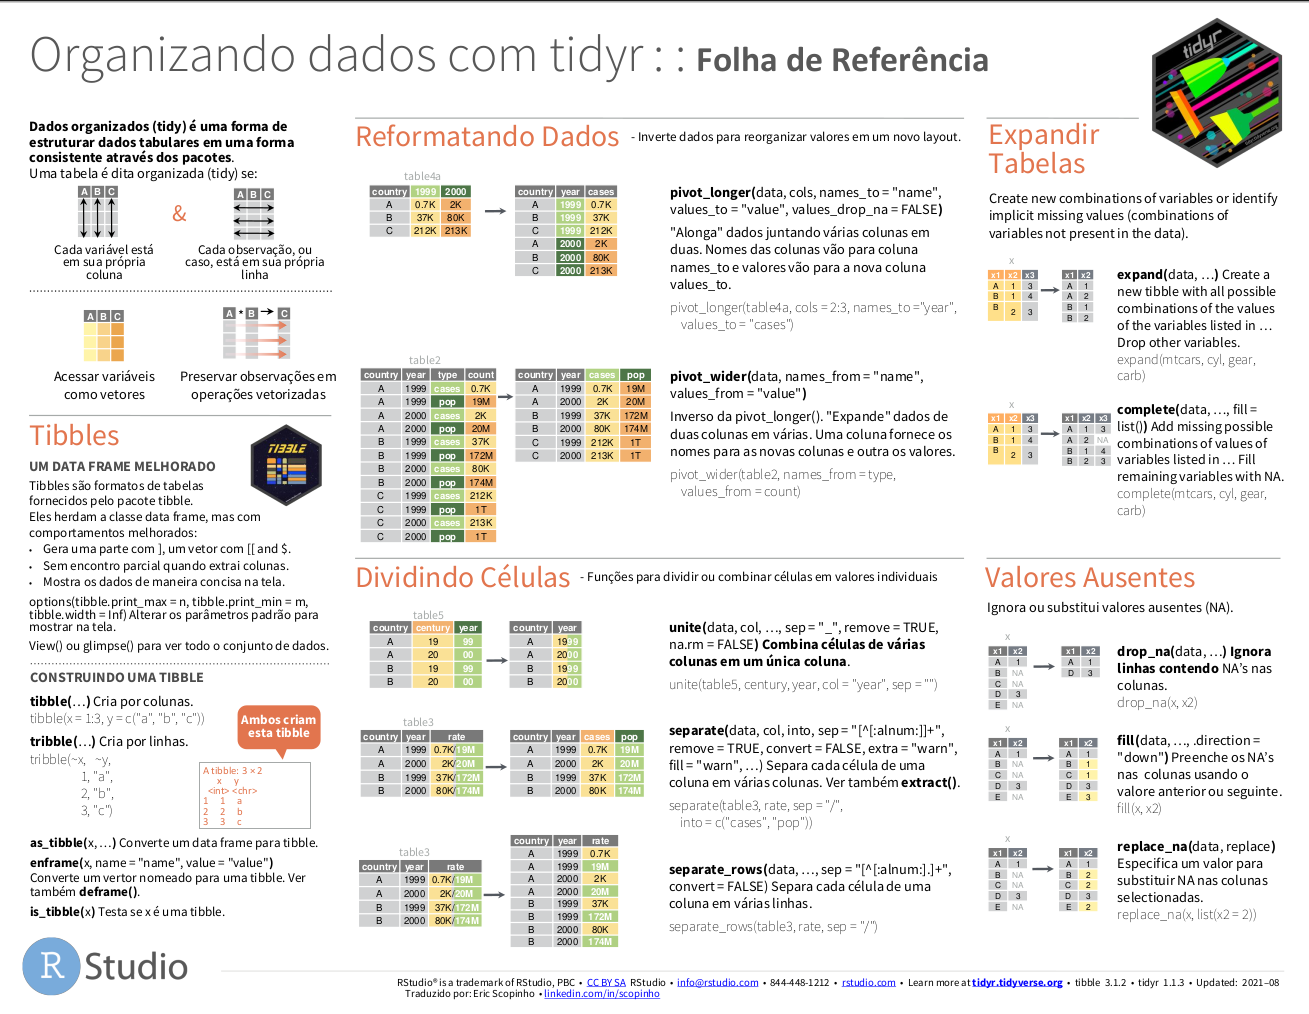
\includegraphics{Organizacao/images/cs-tidyr-01.png}}

}

\end{figure}

\begin{figure}

{\centering 

\href{images/cs-tidyr-02.png}{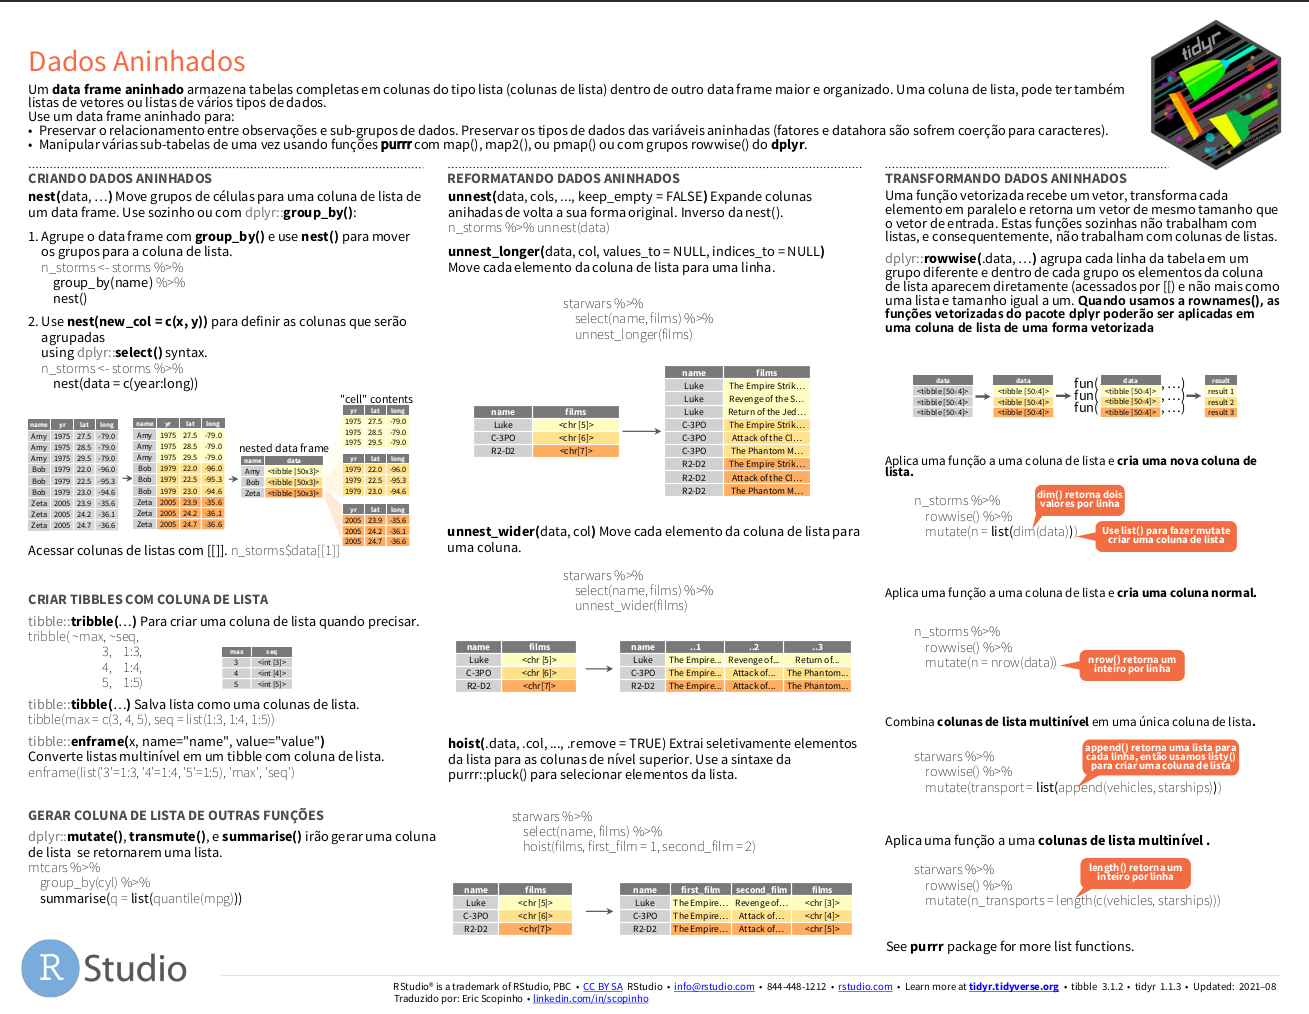
\includegraphics{Organizacao/images/cs-tidyr-02.png}}

}

\end{figure}

\hypertarget{conjunto-de-dados}{%
\subsection{Conjunto de Dados}\label{conjunto-de-dados}}

Para a maioria dos exemplos utilizaremos as bases de dados
\textbf{mtcars, storms} e \textbf{starwars} provenientes do pacote
\textbf{datasets e dplyr e} também algumas tabelas (\textbf{Table1},
\textbf{2, 3, 4a, 4b e 5}) que vem com o pacote \textbf{tidyr}.

\begin{center}\rule{0.5\linewidth}{0.5pt}\end{center}

\textbf{MTCARS}: Dados de consumo de combustível, performance e design
de 32 automóveis ( \emph{1974 Motor Trend US magazine})

\begin{Shaded}
\begin{Highlighting}[]
\NormalTok{mtcars }\SpecialCharTok{|\textgreater{}} 
  \FunctionTok{head}\NormalTok{ () }
\end{Highlighting}
\end{Shaded}

\begin{verbatim}
                   mpg cyl disp  hp drat    wt  qsec vs am gear carb
Mazda RX4         21.0   6  160 110 3.90 2.620 16.46  0  1    4    4
Mazda RX4 Wag     21.0   6  160 110 3.90 2.875 17.02  0  1    4    4
Datsun 710        22.8   4  108  93 3.85 2.320 18.61  1  1    4    1
Hornet 4 Drive    21.4   6  258 110 3.08 3.215 19.44  1  0    3    1
Hornet Sportabout 18.7   8  360 175 3.15 3.440 17.02  0  0    3    2
Valiant           18.1   6  225 105 2.76 3.460 20.22  1  0    3    1
\end{verbatim}

\begin{center}\rule{0.5\linewidth}{0.5pt}\end{center}

\textbf{STORMS}: Dados de furacões entre 1975-2020 medidos a cada 6
horas durante cada tempestade ( \emph{NOAA Atlantic hurricane database}
),

\begin{Shaded}
\begin{Highlighting}[]
\NormalTok{storms }\SpecialCharTok{|\textgreater{}} 
  \FunctionTok{head}\NormalTok{ () }
\end{Highlighting}
\end{Shaded}

\begin{verbatim}
# A tibble: 6 x 13
  name   year month   day  hour   lat  long status categ~1  wind press~2 tropi~3
  <chr> <dbl> <dbl> <int> <dbl> <dbl> <dbl> <chr>  <ord>   <int>   <int>   <int>
1 Amy    1975     6    27     0  27.5 -79   tropi~ -1         25    1013      NA
2 Amy    1975     6    27     6  28.5 -79   tropi~ -1         25    1013      NA
3 Amy    1975     6    27    12  29.5 -79   tropi~ -1         25    1013      NA
4 Amy    1975     6    27    18  30.5 -79   tropi~ -1         25    1013      NA
5 Amy    1975     6    28     0  31.5 -78.8 tropi~ -1         25    1012      NA
6 Amy    1975     6    28     6  32.4 -78.7 tropi~ -1         25    1012      NA
# ... with 1 more variable: hurricane_force_diameter <int>, and abbreviated
#   variable names 1: category, 2: pressure, 3: tropicalstorm_force_diameter
# i Use `colnames()` to see all variable names
\end{verbatim}

\begin{center}\rule{0.5\linewidth}{0.5pt}\end{center}

\textbf{STARWARS}: Dados dos personagens de STAR WARS

\begin{Shaded}
\begin{Highlighting}[]
\NormalTok{starwars }\SpecialCharTok{|\textgreater{}} 
  \FunctionTok{select}\NormalTok{(}\DecValTok{1}\SpecialCharTok{:}\DecValTok{8}\NormalTok{) }\SpecialCharTok{|\textgreater{}} 
  \FunctionTok{head}\NormalTok{()}
\end{Highlighting}
\end{Shaded}

\begin{verbatim}
# A tibble: 6 x 8
  name           height  mass hair_color  skin_color  eye_color birth_year sex  
  <chr>           <int> <dbl> <chr>       <chr>       <chr>          <dbl> <chr>
1 Luke Skywalker    172    77 blond       fair        blue            19   male 
2 C-3PO             167    75 <NA>        gold        yellow         112   none 
3 R2-D2              96    32 <NA>        white, blue red             33   none 
4 Darth Vader       202   136 none        white       yellow          41.9 male 
5 Leia Organa       150    49 brown       light       brown           19   fema~
6 Owen Lars         178   120 brown, grey light       blue            52   male 
\end{verbatim}

\textbf{TABELAS EXEMPLOS} - Table1, 2, 3, 4a, 4b e 5

\hypertarget{table1}{%
\subsubsection{Table1}\label{table1}}

\begin{Shaded}
\begin{Highlighting}[]
\NormalTok{table1}
\end{Highlighting}
\end{Shaded}

\begin{verbatim}
# A tibble: 6 x 4
  country      year  cases population
  <chr>       <int>  <int>      <int>
1 Afghanistan  1999    745   19987071
2 Afghanistan  2000   2666   20595360
3 Brazil       1999  37737  172006362
4 Brazil       2000  80488  174504898
5 China        1999 212258 1272915272
6 China        2000 213766 1280428583
\end{verbatim}

\hypertarget{table2}{%
\subsubsection{Table2}\label{table2}}

\begin{Shaded}
\begin{Highlighting}[]
\NormalTok{table2}
\end{Highlighting}
\end{Shaded}

\begin{verbatim}
# A tibble: 12 x 4
   country      year type            count
   <chr>       <int> <chr>           <int>
 1 Afghanistan  1999 cases             745
 2 Afghanistan  1999 population   19987071
 3 Afghanistan  2000 cases            2666
 4 Afghanistan  2000 population   20595360
 5 Brazil       1999 cases           37737
 6 Brazil       1999 population  172006362
 7 Brazil       2000 cases           80488
 8 Brazil       2000 population  174504898
 9 China        1999 cases          212258
10 China        1999 population 1272915272
11 China        2000 cases          213766
12 China        2000 population 1280428583
\end{verbatim}

\hypertarget{table3}{%
\subsubsection{Table3}\label{table3}}

\begin{Shaded}
\begin{Highlighting}[]
\NormalTok{table3}
\end{Highlighting}
\end{Shaded}

\begin{verbatim}
# A tibble: 6 x 3
  country      year rate             
* <chr>       <int> <chr>            
1 Afghanistan  1999 745/19987071     
2 Afghanistan  2000 2666/20595360    
3 Brazil       1999 37737/172006362  
4 Brazil       2000 80488/174504898  
5 China        1999 212258/1272915272
6 China        2000 213766/1280428583
\end{verbatim}

\hypertarget{table4a}{%
\subsubsection{Table4a}\label{table4a}}

\begin{Shaded}
\begin{Highlighting}[]
\NormalTok{table4a}
\end{Highlighting}
\end{Shaded}

\begin{verbatim}
# A tibble: 3 x 3
  country     `1999` `2000`
* <chr>        <int>  <int>
1 Afghanistan    745   2666
2 Brazil       37737  80488
3 China       212258 213766
\end{verbatim}

\hypertarget{table4b}{%
\subsubsection{Table4b}\label{table4b}}

\begin{Shaded}
\begin{Highlighting}[]
\NormalTok{table4b}
\end{Highlighting}
\end{Shaded}

\begin{verbatim}
# A tibble: 3 x 3
  country         `1999`     `2000`
* <chr>            <int>      <int>
1 Afghanistan   19987071   20595360
2 Brazil       172006362  174504898
3 China       1272915272 1280428583
\end{verbatim}

\hypertarget{table5}{%
\subsubsection{Table5}\label{table5}}

\begin{Shaded}
\begin{Highlighting}[]
\NormalTok{table5}
\end{Highlighting}
\end{Shaded}

\begin{verbatim}
# A tibble: 6 x 4
  country     century year  rate             
* <chr>       <chr>   <chr> <chr>            
1 Afghanistan 19      99    745/19987071     
2 Afghanistan 20      00    2666/20595360    
3 Brazil      19      99    37737/172006362  
4 Brazil      20      00    80488/174504898  
5 China       19      99    212258/1272915272
6 China       20      00    213766/1280428583
\end{verbatim}

\begin{tcolorbox}[enhanced jigsaw, rightrule=.15mm, arc=.35mm, coltitle=black, colframe=quarto-callout-note-color-frame, opacityback=0, toprule=.15mm, left=2mm, breakable, colback=white, bottomtitle=1mm, leftrule=.75mm, title=\textcolor{quarto-callout-note-color}{\faInfo}\hspace{0.5em}{Nota}, colbacktitle=quarto-callout-note-color!10!white, titlerule=0mm, bottomrule=.15mm, toptitle=1mm, opacitybacktitle=0.6]
\emph{O termo \uline{data-frame} descrito ao longo deste texto, é
utilizado de forma livre para objetos do tipo data.frame, tibble, entre
outros. Pense como se fosse uma tabela de um banco de dados e/ou uma
planilha do MS Excel, contendo linhas e colunas. Apesar de não ser
rigorosamente igual à uma tabela, muitas vezes usaremos estes termos de
forma intercambiável para facilitar o entendimento de iniciantes.}
\end{tcolorbox}

\hypertarget{dados-organizados}{%
\subsection{Dados Organizados}\label{dados-organizados}}

Conforme visto anteriorment, dados organizados (\emph{tidy}) são
estruturados onde:

Cada \textbf{variável} está em sua própria \textbf{coluna} e cada
\textbf{observação} está em sua própria \textbf{linha}.

\includegraphics{Organizacao/images/tidy_data01.png}

As \textbf{variáveis} (ou colunas) são acessadas como vetores.

Os \textbf{observações} (ou linhas) são preservadas em operações
vetorizadas, ou seja, quando utilizamos funções que recebem vetores na
entrada e retornam vetores na sua saída.

\hypertarget{tibbles}{%
\section{Tibbles}\label{tibbles}}

Podemos considerar que ``\textbf{Tibbles}'' são objetos similares aos
``\textbf{Data Frames}'', porém com algumas melhorias/vantagens. Estes
objetos são fornecidos pelo packago \textbf{tibble}. Eles herdam a
classe data frame, mas possuem alguns comportamentos melhorados, como:

\begin{itemize}
\item
  Extrai parte de um tibble usando colchetes {]} e um vetor com duplo
  colchetes {]}{]} ou \$
\item
  Sem encontros parciais quando extraindo partes das colunas
\item
  Mostram uma resumo mais amigável na tela quando pedimos suas
  informações. Use options(tibble.print\_max = n, tibble.print\_min = m,
  tibble.width = Inf) para controlar a saída padrão.
\item
  As funções View() ou glimpse() permitem visualizar todo o conjunto de
  dados.
\end{itemize}

Por exemplo, se tivermos um tibble (ex starwars) e quisermos acessar a
coluna ``name'', e obter um \textbf{vetor}, podemos usar:

\begin{Shaded}
\begin{Highlighting}[]
\NormalTok{starwars[[}\StringTok{"name"}\NormalTok{]] }\CommentTok{\#Por nome com [[  ]]}
\NormalTok{starwars}\SpecialCharTok{$}\NormalTok{name      }\CommentTok{\#Por nome com $}
\NormalTok{starwars[[}\DecValTok{1}\NormalTok{]]      }\CommentTok{\#Por numero da coluna com [[  ]]}
\end{Highlighting}
\end{Shaded}

Já se tivermos um tibble (ex starwars) e quisermos acessar a coluna
``name'', e obter um \textbf{tibble}, podemos usar:

\begin{Shaded}
\begin{Highlighting}[]
\NormalTok{starwars[ , }\DecValTok{1}\NormalTok{]            }\CommentTok{\#Por numero com [   ]}
\FunctionTok{select}\NormalTok{ (starwars, }\DecValTok{3}\NormalTok{)      }\CommentTok{\#Por numero usando select()}
\FunctionTok{select}\NormalTok{ (starwars, name)   }\CommentTok{\#Por nome usando select()}
\end{Highlighting}
\end{Shaded}

\hypertarget{criando-tibble}{%
\subsection{Criando tibble}\label{criando-tibble}}

Podemos utilziar as funções tibble() ou tribble() para criar a mesma
tabela. A diferença é apenas na forma em que os parêmetros são
utilizados.

\hypertarget{tibble}{%
\subsubsection{tibble}\label{tibble}}

Use para criar um tibble por colunas.

\begin{Shaded}
\begin{Highlighting}[]
\FunctionTok{tibble}\NormalTok{(}\AttributeTok{x =} \DecValTok{1}\SpecialCharTok{:}\DecValTok{3}\NormalTok{, }\AttributeTok{y =} \FunctionTok{c}\NormalTok{(}\StringTok{"a"}\NormalTok{, }\StringTok{"b"}\NormalTok{, }\StringTok{"c"}\NormalTok{))}
\end{Highlighting}
\end{Shaded}

\begin{verbatim}
# A tibble: 3 x 2
      x y    
  <int> <chr>
1     1 a    
2     2 b    
3     3 c    
\end{verbatim}

\hypertarget{tribble}{%
\subsubsection{tribble}\label{tribble}}

Use para criar um tibble por linhas.

\begin{Shaded}
\begin{Highlighting}[]
\FunctionTok{tribble}\NormalTok{(}\SpecialCharTok{\textasciitilde{}}\NormalTok{x, }\SpecialCharTok{\textasciitilde{}}\NormalTok{y, }
        \DecValTok{1}\NormalTok{, }\StringTok{"a"}\NormalTok{,}
        \DecValTok{2}\NormalTok{, }\StringTok{"b"}\NormalTok{,}
        \DecValTok{3}\NormalTok{, }\StringTok{"c"}\NormalTok{,}
        \DecValTok{4}\NormalTok{, }\StringTok{"d"}\NormalTok{)}
\end{Highlighting}
\end{Shaded}

\begin{verbatim}
# A tibble: 4 x 2
      x y    
  <dbl> <chr>
1     1 a    
2     2 b    
3     3 c    
4     4 d    
\end{verbatim}

\hypertarget{as_tibble}{%
\subsubsection{as\_tibble}\label{as_tibble}}

Use para converter um data frame para um tibble.

Por exemplo, para converter o data frame MTCARS para um tibble, fazemos:

\begin{Shaded}
\begin{Highlighting}[]
\FunctionTok{as\_tibble}\NormalTok{(mtcars)}
\end{Highlighting}
\end{Shaded}

\begin{verbatim}
# A tibble: 32 x 11
     mpg   cyl  disp    hp  drat    wt  qsec    vs    am  gear  carb
   <dbl> <dbl> <dbl> <dbl> <dbl> <dbl> <dbl> <dbl> <dbl> <dbl> <dbl>
 1  21       6  160    110  3.9   2.62  16.5     0     1     4     4
 2  21       6  160    110  3.9   2.88  17.0     0     1     4     4
 3  22.8     4  108     93  3.85  2.32  18.6     1     1     4     1
 4  21.4     6  258    110  3.08  3.22  19.4     1     0     3     1
 5  18.7     8  360    175  3.15  3.44  17.0     0     0     3     2
 6  18.1     6  225    105  2.76  3.46  20.2     1     0     3     1
 7  14.3     8  360    245  3.21  3.57  15.8     0     0     3     4
 8  24.4     4  147.    62  3.69  3.19  20       1     0     4     2
 9  22.8     4  141.    95  3.92  3.15  22.9     1     0     4     2
10  19.2     6  168.   123  3.92  3.44  18.3     1     0     4     4
# ... with 22 more rows
# i Use `print(n = ...)` to see more rows
\end{verbatim}

\hypertarget{enframe}{%
\subsubsection{enframe}\label{enframe}}

Use para converter um vetor para um tibble. Use deframe() parta fazer o
inverso.

\hypertarget{is_tibble}{%
\subsubsection{is\_tibble}\label{is_tibble}}

Use para saber se um objeto é um tibble ou não.

\begin{Shaded}
\begin{Highlighting}[]
\FunctionTok{is\_tibble}\NormalTok{(mtcars)}
\end{Highlighting}
\end{Shaded}

\begin{verbatim}
[1] FALSE
\end{verbatim}

\hypertarget{reformatando-dados}{%
\section{Reformatando Dados}\label{reformatando-dados}}

Muitas vezes, os dados que recebemos não estão organizados (tidy) da
maneira como vimos na seção
\protect\hyperlink{dados-organizados-e-canalizauxe7uxe3o}{Dados
Organizados e Canalização}. Para casos onde temos, por exemplo, as
variáveis em linhas e/ou observações em colunas, etc, precisamos fazer
uma ação conhecida como ``pivotagem''. Pivotar dados, no contexto do
tidyr, significa ajustar linhas em colunas e/ou colunas em linhas, de
forma a obtermos nossos dados da maneira organizada (tidy).

Veja, por exemplo, nossa tabela 1 (table1). Ela está em um formato
organizado, pois possui cada variável em uma coluna e cada observações
em sua linha, com os valores nas células.

\begin{Shaded}
\begin{Highlighting}[]
\NormalTok{table1}
\end{Highlighting}
\end{Shaded}

\begin{verbatim}
# A tibble: 6 x 4
  country      year  cases population
  <chr>       <int>  <int>      <int>
1 Afghanistan  1999    745   19987071
2 Afghanistan  2000   2666   20595360
3 Brazil       1999  37737  172006362
4 Brazil       2000  80488  174504898
5 China        1999 212258 1272915272
6 China        2000 213766 1280428583
\end{verbatim}

\hypertarget{pivot_longer}{%
\subsubsection{pivot\_longer}\label{pivot_longer}}

Use para ``pivotar'' os dados das colunas para as linhas,
\textbf{alongando} a tabela, juntando várias colunas em duas, sendo uma
a colunas que receberá os nomes das colunas e outra que recebera os
valores das colunas.

Por exemplo, vejamos nossa tabela 4 (table4).

\begin{Shaded}
\begin{Highlighting}[]
\NormalTok{table4a}
\end{Highlighting}
\end{Shaded}

\begin{verbatim}
# A tibble: 3 x 3
  country     `1999` `2000`
* <chr>        <int>  <int>
1 Afghanistan    745   2666
2 Brazil       37737  80488
3 China       212258 213766
\end{verbatim}

Observe que temos uma variável (potencialmente ``Ano'') que está na
colunas 2 e 3 da tabela. Temos também outra variável (potencialmente
``Numero\_de\_Casos'' que está nas células da tabela.

Para organizar esta tabela em nosso formato ``tidy'', devemos pegar
estas duas colunas e usar a função pivot\_longer definindo os nomes para
as respectivas variáveis (ex: ano e num\_caso).

\begin{Shaded}
\begin{Highlighting}[]
\FunctionTok{pivot\_longer}\NormalTok{(table4a, }\AttributeTok{cols =} \DecValTok{2}\SpecialCharTok{:}\DecValTok{3}\NormalTok{, }\AttributeTok{names\_to =}\StringTok{"ano"}\NormalTok{,}
\AttributeTok{values\_to =} \StringTok{"num\_casos"}\NormalTok{) }
\end{Highlighting}
\end{Shaded}

\begin{verbatim}
# A tibble: 6 x 3
  country     ano   num_casos
  <chr>       <chr>     <int>
1 Afghanistan 1999        745
2 Afghanistan 2000       2666
3 Brazil      1999      37737
4 Brazil      2000      80488
5 China       1999     212258
6 China       2000     213766
\end{verbatim}

\hypertarget{pivot_wider}{%
\subsubsection{pivot\_wider}\label{pivot_wider}}

Use para ``pivotar'' os dados das linhas para as colunas,
\textbf{expandindo} a tabela gerando novas colunas.

Vejamos o caso da tabela 2 (table2).

\begin{Shaded}
\begin{Highlighting}[]
\NormalTok{table2}
\end{Highlighting}
\end{Shaded}

\begin{verbatim}
# A tibble: 12 x 4
   country      year type            count
   <chr>       <int> <chr>           <int>
 1 Afghanistan  1999 cases             745
 2 Afghanistan  1999 population   19987071
 3 Afghanistan  2000 cases            2666
 4 Afghanistan  2000 population   20595360
 5 Brazil       1999 cases           37737
 6 Brazil       1999 population  172006362
 7 Brazil       2000 cases           80488
 8 Brazil       2000 population  174504898
 9 China        1999 cases          212258
10 China        1999 population 1272915272
11 China        2000 cases          213766
12 China        2000 population 1280428583
\end{verbatim}

Neste exemplo, vemos que as variáveis casos (cases) e população
(population) estão nas linhas e não nas colunas. Para deixarmos os dados
organizados (tidy), devemos ``expandir'' a tabela, fazendo com que os
dados de duas colunas sejam expandidos em vaŕias colunas. Os nomes das
novas colunas virão de uma colunas e os valores da outra coluna. Veja:

\begin{Shaded}
\begin{Highlighting}[]
\NormalTok{table2 }\SpecialCharTok{|\textgreater{}} 
  \FunctionTok{pivot\_wider}\NormalTok{(}\AttributeTok{names\_from =}\NormalTok{ type, }\AttributeTok{values\_from =}\NormalTok{ count) }
\end{Highlighting}
\end{Shaded}

\begin{verbatim}
# A tibble: 6 x 4
  country      year  cases population
  <chr>       <int>  <int>      <int>
1 Afghanistan  1999    745   19987071
2 Afghanistan  2000   2666   20595360
3 Brazil       1999  37737  172006362
4 Brazil       2000  80488  174504898
5 China        1999 212258 1272915272
6 China        2000 213766 1280428583
\end{verbatim}

\hypertarget{expandindo-tabelas}{%
\section{Expandindo Tabelas}\label{expandindo-tabelas}}

Em algumas situações, precisamos criar novas combinações das variáveis
ou identificar valores ausentes implícitos, ou seja, combinações de
variáveis não presentes nos dados.

Para isto, temos as funções \textbf{expand}() e \textbf{complete}().

\hypertarget{expand}{%
\subsubsection{expand}\label{expand}}

Use para criar um novo tibble com todas as possibilidades de combinações
dos valores das variáveis passadas para a função expand(),
\textbf{ignorando} as demais variáveis.

Por exemplo, se quisermos obter todas as combinações possíveis entre o
número de cilindros (cyl), marchas (gear) e numero de carburadores
(carb) da tabela mtcars, e ignorar todas as demais variáveis da tabela,
podemos usar:

\begin{Shaded}
\begin{Highlighting}[]
\NormalTok{mtcars }\SpecialCharTok{|\textgreater{}} 
  \FunctionTok{expand}\NormalTok{(cyl, gear, carb) }
\end{Highlighting}
\end{Shaded}

\begin{verbatim}
# A tibble: 54 x 3
     cyl  gear  carb
   <dbl> <dbl> <dbl>
 1     4     3     1
 2     4     3     2
 3     4     3     3
 4     4     3     4
 5     4     3     6
 6     4     3     8
 7     4     4     1
 8     4     4     2
 9     4     4     3
10     4     4     4
# ... with 44 more rows
# i Use `print(n = ...)` to see more rows
\end{verbatim}

Observe que não há na tabela original (mtcars) um veículo de 4 cilindros
e 8 carburadores, porém esta combinação foi possível usando a função
expand().

\hypertarget{complete}{%
\subsubsection{complete}\label{complete}}

Use para criar um novo tibble com todas as possibilidades de combinações
dos valores das variáveis passadas para a função expand(),
\textbf{colocando NA} nas demais variáveis.

Por exemplo, se quisermos obter todas as combinações possíveis entre o
número de cilindros (cyl), marchas (gear) e numero de carburadores
(carb) da tabela mtcars, e colocar NA para as demais variáveis em que a
combinação não exista, podemos usar:

\begin{Shaded}
\begin{Highlighting}[]
\NormalTok{mtcars }\SpecialCharTok{|\textgreater{}} 
  \FunctionTok{complete}\NormalTok{(cyl, gear, carb) }
\end{Highlighting}
\end{Shaded}

\begin{verbatim}
# A tibble: 74 x 11
     cyl  gear  carb   mpg  disp    hp  drat    wt  qsec    vs    am
   <dbl> <dbl> <dbl> <dbl> <dbl> <dbl> <dbl> <dbl> <dbl> <dbl> <dbl>
 1     4     3     1  21.5 120.     97  3.7   2.46  20.0     1     0
 2     4     3     2  NA    NA      NA NA    NA     NA      NA    NA
 3     4     3     3  NA    NA      NA NA    NA     NA      NA    NA
 4     4     3     4  NA    NA      NA NA    NA     NA      NA    NA
 5     4     3     6  NA    NA      NA NA    NA     NA      NA    NA
 6     4     3     8  NA    NA      NA NA    NA     NA      NA    NA
 7     4     4     1  22.8 108      93  3.85  2.32  18.6     1     1
 8     4     4     1  32.4  78.7    66  4.08  2.2   19.5     1     1
 9     4     4     1  33.9  71.1    65  4.22  1.84  19.9     1     1
10     4     4     1  27.3  79      66  4.08  1.94  18.9     1     1
# ... with 64 more rows
# i Use `print(n = ...)` to see more rows
\end{verbatim}

\hypertarget{combinando-e-dividindo-celulas}{%
\section{Combinando e Dividindo
Celulas}\label{combinando-e-dividindo-celulas}}

Use as funções a seguir para dividir ou combinar células da tabela em
valores individuais isolados.

\hypertarget{unite}{%
\subsubsection{unite}\label{unite}}

Use para combinar celulas de diversas colunas em uma única coluna.

Vejamos com é a tabela 5 (table5) em seu formato original:

\begin{Shaded}
\begin{Highlighting}[]
\NormalTok{table5 }
\end{Highlighting}
\end{Shaded}

\begin{verbatim}
# A tibble: 6 x 4
  country     century year  rate             
* <chr>       <chr>   <chr> <chr>            
1 Afghanistan 19      99    745/19987071     
2 Afghanistan 20      00    2666/20595360    
3 Brazil      19      99    37737/172006362  
4 Brazil      20      00    80488/174504898  
5 China       19      99    212258/1272915272
6 China       20      00    213766/1280428583
\end{verbatim}

Agora queremos unir as colunas ``century'' e ``year'' em uma única
coluna:

\begin{Shaded}
\begin{Highlighting}[]
\NormalTok{table5 }\SpecialCharTok{|\textgreater{}} 
  \FunctionTok{unite}\NormalTok{(century, year, }\AttributeTok{col =} \StringTok{"ano\_completo"}\NormalTok{, }\AttributeTok{sep =} \StringTok{""}\NormalTok{) }
\end{Highlighting}
\end{Shaded}

\begin{verbatim}
# A tibble: 6 x 3
  country     ano_completo rate             
  <chr>       <chr>        <chr>            
1 Afghanistan 1999         745/19987071     
2 Afghanistan 2000         2666/20595360    
3 Brazil      1999         37737/172006362  
4 Brazil      2000         80488/174504898  
5 China       1999         212258/1272915272
6 China       2000         213766/1280428583
\end{verbatim}

\begin{tcolorbox}[enhanced jigsaw, rightrule=.15mm, arc=.35mm, coltitle=black, colframe=quarto-callout-note-color-frame, opacityback=0, toprule=.15mm, left=2mm, breakable, colback=white, bottomtitle=1mm, leftrule=.75mm, title=\textcolor{quarto-callout-note-color}{\faInfo}\hspace{0.5em}{Nota}, colbacktitle=quarto-callout-note-color!10!white, titlerule=0mm, bottomrule=.15mm, toptitle=1mm, opacitybacktitle=0.6]
Veja que as colunas que deram origem à coluna combinada não são
retornadas na saída da função.
\end{tcolorbox}

\hypertarget{separate}{%
\subsubsection{separate}\label{separate}}

Use para dividir cada célula de \textbf{uma coluna} em \textbf{várias
colunas}.

Por exemplo, na tabela 3 (table3), temos uma coluna ``rate'' que possui
daos dos casos e população separados por uma barr (``/''). Neste caso,
podemos utilzar a função separate para dividí-la e criar duas novas
colunas com seus dados separados.

\begin{Shaded}
\begin{Highlighting}[]
\NormalTok{table3 }\SpecialCharTok{|\textgreater{}} 
  \FunctionTok{separate}\NormalTok{(rate, }\AttributeTok{sep =} \StringTok{"/"}\NormalTok{, }
           \AttributeTok{into =} \FunctionTok{c}\NormalTok{(}\StringTok{"casos"}\NormalTok{, }\StringTok{"pop"}\NormalTok{)) }
\end{Highlighting}
\end{Shaded}

\begin{verbatim}
# A tibble: 6 x 4
  country      year casos  pop       
  <chr>       <int> <chr>  <chr>     
1 Afghanistan  1999 745    19987071  
2 Afghanistan  2000 2666   20595360  
3 Brazil       1999 37737  172006362 
4 Brazil       2000 80488  174504898 
5 China        1999 212258 1272915272
6 China        2000 213766 1280428583
\end{verbatim}

\hypertarget{separate_rows}{%
\subsubsection{separate\_rows}\label{separate_rows}}

Use para dividir cada célula de \textbf{uma coluna} em \textbf{várias
linhas}.

É similar a função \href{}{separate}, porém o conteúdo de cada célula
irá para uma linha ao invés de uma colunas.

\begin{Shaded}
\begin{Highlighting}[]
\NormalTok{table3 }\SpecialCharTok{|\textgreater{}} 
  \FunctionTok{separate\_rows}\NormalTok{(rate, }\AttributeTok{sep =} \StringTok{"/"}\NormalTok{) }
\end{Highlighting}
\end{Shaded}

\begin{verbatim}
# A tibble: 12 x 3
   country      year rate      
   <chr>       <int> <chr>     
 1 Afghanistan  1999 745       
 2 Afghanistan  1999 19987071  
 3 Afghanistan  2000 2666      
 4 Afghanistan  2000 20595360  
 5 Brazil       1999 37737     
 6 Brazil       1999 172006362 
 7 Brazil       2000 80488     
 8 Brazil       2000 174504898 
 9 China        1999 212258    
10 China        1999 1272915272
11 China        2000 213766    
12 China        2000 1280428583
\end{verbatim}

\hypertarget{lidando-com-valores-ausentes}{%
\section{Lidando com Valores
Ausentes}\label{lidando-com-valores-ausentes}}

Muitas vezes precisamos \textbf{ignorar} ou \textbf{substituir} valores
ausentes (\textbf{NA}). Para isso, podemos usar as funções drop\_na(),
fill() ou replace\_na()

\hypertarget{drop_na}{%
\subsubsection{drop\_na}\label{drop_na}}

Ignora linhas que possuem valores ausentes (NA) nas colunas.

Por exemplo, na tabela starwars, temos 5 personagens que não possuim cor
de cabelo (hair color):

\begin{Shaded}
\begin{Highlighting}[]
\NormalTok{starwars }\SpecialCharTok{|\textgreater{}} 
  \FunctionTok{select}\NormalTok{(name, hair\_color) }\SpecialCharTok{|\textgreater{}} 
  \FunctionTok{filter}\NormalTok{(}\FunctionTok{is.na}\NormalTok{(hair\_color))}
\end{Highlighting}
\end{Shaded}

\begin{verbatim}
# A tibble: 5 x 2
  name                  hair_color
  <chr>                 <chr>     
1 C-3PO                 <NA>      
2 R2-D2                 <NA>      
3 R5-D4                 <NA>      
4 Greedo                <NA>      
5 Jabba Desilijic Tiure <NA>      
\end{verbatim}

Se pedirmos para listar todos os personagens e utilizarmos a função
drop\_na(), estes 5 personagens não serão listados:

\begin{Shaded}
\begin{Highlighting}[]
\NormalTok{starwars }\SpecialCharTok{|\textgreater{}} 
  \FunctionTok{select}\NormalTok{(name, hair\_color) }\SpecialCharTok{|\textgreater{}} 
  \FunctionTok{drop\_na}\NormalTok{()}
\end{Highlighting}
\end{Shaded}

\begin{verbatim}
# A tibble: 82 x 2
   name               hair_color   
   <chr>              <chr>        
 1 Luke Skywalker     blond        
 2 Darth Vader        none         
 3 Leia Organa        brown        
 4 Owen Lars          brown, grey  
 5 Beru Whitesun lars brown        
 6 Biggs Darklighter  black        
 7 Obi-Wan Kenobi     auburn, white
 8 Anakin Skywalker   blond        
 9 Wilhuff Tarkin     auburn, grey 
10 Chewbacca          brown        
# ... with 72 more rows
# i Use `print(n = ...)` to see more rows
\end{verbatim}

\hypertarget{fill}{%
\subsubsection{fill}\label{fill}}

Use para substituir o valores ausente (NA) da coluna pelo último valor
disponível em linhas anteriores ou posteriores.

Por exemplo:

Como vimos no exemplo da função \href{}{drop\_na}, temos 5 personagens
de starwars que não possuem cor de cabelo preenchido.

Digamos que decidimos substituir estes NAs pelo cor de cabelo do
personagem anterior disponível. Para isso, faremos:

\begin{Shaded}
\begin{Highlighting}[]
\NormalTok{starwars }\SpecialCharTok{|\textgreater{}} 
  \FunctionTok{select}\NormalTok{ (name, hair\_color) }\SpecialCharTok{|\textgreater{}} 
  \FunctionTok{fill}\NormalTok{(hair\_color)}
\end{Highlighting}
\end{Shaded}

\begin{verbatim}
# A tibble: 87 x 2
   name               hair_color   
   <chr>              <chr>        
 1 Luke Skywalker     blond        
 2 C-3PO              blond        
 3 R2-D2              blond        
 4 Darth Vader        none         
 5 Leia Organa        brown        
 6 Owen Lars          brown, grey  
 7 Beru Whitesun lars brown        
 8 R5-D4              brown        
 9 Biggs Darklighter  black        
10 Obi-Wan Kenobi     auburn, white
# ... with 77 more rows
# i Use `print(n = ...)` to see more rows
\end{verbatim}

Veja que o personagem C-3PO que tinha a cor de cabelo não preenchida,
agora está como loiro (blond), pois o personagem anteriormente
preenchido, era o Luke Skywalker, que tinha a cor de cabelo loiro
(blond). Já o personagem R5-D4, teve sua cor de cabelo preenchida de
marron (brown), pois o personagem anterior Beru Whitesun lars, tinha o
cabelo marron (brown).

\hypertarget{replace_na}{%
\subsubsection{replace\_na}\label{replace_na}}

Use para substituir os valores de NA por um valor específico.

Por exemplo, vamos substituir a cor de cabelo dos personagens que tem NA
na coluna ``hair\_color'' pela cor azul (blue).

\begin{Shaded}
\begin{Highlighting}[]
\NormalTok{starwars }\SpecialCharTok{|\textgreater{}} 
  \FunctionTok{select}\NormalTok{(name, hair\_color) }\SpecialCharTok{|\textgreater{}} 
  \FunctionTok{replace\_na}\NormalTok{(}\FunctionTok{list}\NormalTok{(}\AttributeTok{hair\_color =} \StringTok{"blue"}\NormalTok{))}
\end{Highlighting}
\end{Shaded}

\begin{verbatim}
# A tibble: 87 x 2
   name               hair_color   
   <chr>              <chr>        
 1 Luke Skywalker     blond        
 2 C-3PO              blue         
 3 R2-D2              blue         
 4 Darth Vader        none         
 5 Leia Organa        brown        
 6 Owen Lars          brown, grey  
 7 Beru Whitesun lars brown        
 8 R5-D4              blue         
 9 Biggs Darklighter  black        
10 Obi-Wan Kenobi     auburn, white
# ... with 77 more rows
# i Use `print(n = ...)` to see more rows
\end{verbatim}

\begin{tcolorbox}[enhanced jigsaw, rightrule=.15mm, arc=.35mm, coltitle=black, colframe=quarto-callout-warning-color-frame, opacityback=0, toprule=.15mm, left=2mm, breakable, colback=white, bottomtitle=1mm, leftrule=.75mm, title=\textcolor{quarto-callout-warning-color}{\faExclamationTriangle}\hspace{0.5em}{Aviso}, colbacktitle=quarto-callout-warning-color!10!white, titlerule=0mm, bottomrule=.15mm, toptitle=1mm, opacitybacktitle=0.6]
Veja que a função replace\_na, recebe uma lista de valores (list()) se
os dados passados no primeiro parâmetro é um data frame.
\end{tcolorbox}

\hypertarget{dados-aninhados}{%
\section{Dados Aninhados}\label{dados-aninhados}}

\hypertarget{introduuxe7uxe3o-3}{%
\subsection{Introdução}\label{introduuxe7uxe3o-3}}

Um data frame aninhado (nested) é aquela que possui tabelas completas em
colunas do tipo lista (colunas de lista) dentro de outro data frame
maior e organizado. Uma coluna de lista, podem ser também listas de
vetores ou listas de vários tipos de dados.

Alguns uso de um data frame de dados aninhados são:

\begin{itemize}
\item
  Preservar o relacionamento entre observações e sub-grupos de dados.
\item
  Preservar o tipo da variável aninhada (factors e datetime não viram
  caracteres por exemplo).
\item
  Manipular várias sub-tabelas de uma vez com funcções do pacote purrr
  como map(), map2() ou pmap() ou com a rowwise() do pacote dplyr.
\end{itemize}

\hypertarget{criando-dados-aninhados}{%
\subsection{Criando dados Aninhados}\label{criando-dados-aninhados}}

\hypertarget{nest}{%
\subsubsection{nest}\label{nest}}

Use para mover grupos de células para uma coluna de lista de um data
frame. Pode ser usada sozinha ou em conjunto com a grupo\_by().

\textbf{Exemplo 1: nest() com groupg\_by()}

Digamos que gostaríamos ter uma linha para cada furacão de nosso data
frame (storms) e em uma coluna de lista, uma tabela dos dados do
respectivo furação. Para isso, podemos utilizar a função nest() em
conjunto com a função group\_by(). Veja abaixo:

\begin{Shaded}
\begin{Highlighting}[]
\NormalTok{n\_storms }\OtherTok{\textless{}{-}}\NormalTok{ storms  }\SpecialCharTok{|\textgreater{}} 
  \FunctionTok{group\_by}\NormalTok{(name) }\SpecialCharTok{|\textgreater{}} 
  \FunctionTok{nest}\NormalTok{()}
\FunctionTok{head}\NormalTok{(n\_storms, }\DecValTok{15}\NormalTok{)}
\end{Highlighting}
\end{Shaded}

\begin{verbatim}
# A tibble: 15 x 2
# Groups:   name [15]
   name      data               
   <chr>     <list>             
 1 Amy       <tibble [30 x 12]> 
 2 Caroline  <tibble [33 x 12]> 
 3 Doris     <tibble [23 x 12]> 
 4 Belle     <tibble [18 x 12]> 
 5 Gloria    <tibble [125 x 12]>
 6 Anita     <tibble [20 x 12]> 
 7 Clara     <tibble [24 x 12]> 
 8 Evelyn    <tibble [9 x 12]>  
 9 Amelia    <tibble [6 x 12]>  
10 Bess      <tibble [13 x 12]> 
11 Cora      <tibble [19 x 12]> 
12 Juliet    <tibble [16 x 12]> 
13 Ana       <tibble [100 x 12]>
14 Bob       <tibble [71 x 12]> 
15 Claudette <tibble [180 x 12]>
\end{verbatim}

Observe que na coluna ``data'', temos um objeto
\textless tibble\textgreater{} para grupo criado pela função group\_by.
A função nest() aninhou todas as demais variáveis nestas pequenas
tabelas para cada um deles e armazenou na coluna do tipo lista.

Para acessar a tibble gerada para o primeiro grupo (furacão ``Amy'' na
primeira linha acima), podemos fazer:

\begin{Shaded}
\begin{Highlighting}[]
\NormalTok{n\_storms}\SpecialCharTok{$}\NormalTok{data[[}\DecValTok{1}\NormalTok{]] }
\end{Highlighting}
\end{Shaded}

\begin{verbatim}
# A tibble: 30 x 12
    year month   day  hour   lat  long status      categ~1  wind press~2 tropi~3
   <dbl> <dbl> <int> <dbl> <dbl> <dbl> <chr>       <ord>   <int>   <int>   <int>
 1  1975     6    27     0  27.5 -79   tropical d~ -1         25    1013      NA
 2  1975     6    27     6  28.5 -79   tropical d~ -1         25    1013      NA
 3  1975     6    27    12  29.5 -79   tropical d~ -1         25    1013      NA
 4  1975     6    27    18  30.5 -79   tropical d~ -1         25    1013      NA
 5  1975     6    28     0  31.5 -78.8 tropical d~ -1         25    1012      NA
 6  1975     6    28     6  32.4 -78.7 tropical d~ -1         25    1012      NA
 7  1975     6    28    12  33.3 -78   tropical d~ -1         25    1011      NA
 8  1975     6    28    18  34   -77   tropical d~ -1         30    1006      NA
 9  1975     6    29     0  34.4 -75.8 tropical s~ 0          35    1004      NA
10  1975     6    29     6  34   -74.8 tropical s~ 0          40    1002      NA
# ... with 20 more rows, 1 more variable: hurricane_force_diameter <int>, and
#   abbreviated variable names 1: category, 2: pressure,
#   3: tropicalstorm_force_diameter
# i Use `print(n = ...)` to see more rows, and `colnames()` to see all variable names
\end{verbatim}

Para acessar todas as observações as variáveis ``month'' e ``status''
especificamente, podemos usar:

\begin{Shaded}
\begin{Highlighting}[]
\NormalTok{n\_storms}\SpecialCharTok{$}\NormalTok{data[[}\DecValTok{1}\NormalTok{]][, }\FunctionTok{c}\NormalTok{(}\StringTok{"month"}\NormalTok{, }\StringTok{"status"}\NormalTok{)] }\SpecialCharTok{|\textgreater{}} 
  \FunctionTok{head}\NormalTok{() }
\end{Highlighting}
\end{Shaded}

\begin{verbatim}
# A tibble: 6 x 2
  month status             
  <dbl> <chr>              
1     6 tropical depression
2     6 tropical depression
3     6 tropical depression
4     6 tropical depression
5     6 tropical depression
6     6 tropical depression
\end{verbatim}

\textbf{Exemplo 2: nest() especificando colunas}

Digamos que precisamos especfificar as colunas que gostaríamos de
aninhar em cada linha da coluna de lista. Apenas para simplificar o
exemplo, iremos selecionar com a função selct() apenas as colunas
``name'', ``year'', ``lat'' e ``long''. Depois iremos aninhar as colunas
``year'' até a coluna ``long'' em um coluna de lista chamada ``data''.
Veja a seguir:

\begin{Shaded}
\begin{Highlighting}[]
\NormalTok{n\_storms }\OtherTok{\textless{}{-}}\NormalTok{ storms  }\SpecialCharTok{|\textgreater{}} 
  \FunctionTok{select}\NormalTok{(name, year, lat, long) }\SpecialCharTok{|\textgreater{}} 
  \FunctionTok{nest}\NormalTok{(}\AttributeTok{data =} \FunctionTok{c}\NormalTok{(year}\SpecialCharTok{:}\NormalTok{long))}
\FunctionTok{head}\NormalTok{(n\_storms)}
\end{Highlighting}
\end{Shaded}

\begin{verbatim}
# A tibble: 6 x 2
  name     data              
  <chr>    <list>            
1 Amy      <tibble [30 x 3]> 
2 Caroline <tibble [33 x 3]> 
3 Doris    <tibble [23 x 3]> 
4 Belle    <tibble [18 x 3]> 
5 Gloria   <tibble [125 x 3]>
6 Anita    <tibble [20 x 3]> 
\end{verbatim}

Agora temos as colunas ``year'', ``lat'' e ``long'' aninhadas na coluna
de lista chamada ``data'' para cada observação da coluna ``name''.

Assim como vimos anteriormente, podemos acessar as tibbles da coluna dat
usando {[}{[} {]}{]}. Por exemplo:

\begin{Shaded}
\begin{Highlighting}[]
\NormalTok{n\_storms}\SpecialCharTok{$}\NormalTok{data[[}\DecValTok{1}\NormalTok{]]}
\end{Highlighting}
\end{Shaded}

\begin{verbatim}
# A tibble: 30 x 3
    year   lat  long
   <dbl> <dbl> <dbl>
 1  1975  27.5 -79  
 2  1975  28.5 -79  
 3  1975  29.5 -79  
 4  1975  30.5 -79  
 5  1975  31.5 -78.8
 6  1975  32.4 -78.7
 7  1975  33.3 -78  
 8  1975  34   -77  
 9  1975  34.4 -75.8
10  1975  34   -74.8
# ... with 20 more rows
# i Use `print(n = ...)` to see more rows
\end{verbatim}

\hypertarget{criando-tibbles-com-colunas-de-listas}{%
\subsection{Criando Tibbles com Colunas de
Listas}\label{criando-tibbles-com-colunas-de-listas}}

Para criar um objeto tibble com colunas de lista (list-column), você
pode utilizar as mesmas funções \textbf{tibble}(), \textbf{trible}() e
\textbf{enframe}(), passando uma objeto lista para a coluna.

\hypertarget{tibble-1}{%
\subsubsection{tibble}\label{tibble-1}}

Use para criar uma tibble com uma coluna de lista salvando uma lista na
coluna.

\begin{Shaded}
\begin{Highlighting}[]
\FunctionTok{tibble}\NormalTok{(}\AttributeTok{max=}\FunctionTok{c}\NormalTok{(}\DecValTok{3}\NormalTok{,}\DecValTok{4}\NormalTok{,}\DecValTok{5}\NormalTok{), }\AttributeTok{seq=}\FunctionTok{list}\NormalTok{(}\DecValTok{1}\SpecialCharTok{:}\DecValTok{3}\NormalTok{, }\DecValTok{1}\SpecialCharTok{:}\DecValTok{4}\NormalTok{, }\DecValTok{1}\SpecialCharTok{:}\DecValTok{5}\NormalTok{))}
\end{Highlighting}
\end{Shaded}

\begin{verbatim}
# A tibble: 3 x 2
    max seq      
  <dbl> <list>   
1     3 <int [3]>
2     4 <int [4]>
3     5 <int [5]>
\end{verbatim}

\hypertarget{tribble-1}{%
\subsubsection{tribble}\label{tribble-1}}

Use para criar uma tibble com uma coluna de lista por linhas.

\begin{Shaded}
\begin{Highlighting}[]
\FunctionTok{tribble}\NormalTok{(}\SpecialCharTok{\textasciitilde{}}\NormalTok{max, }\SpecialCharTok{\textasciitilde{}}\NormalTok{seq, }
       \DecValTok{3}\NormalTok{, }\DecValTok{1}\SpecialCharTok{:}\DecValTok{3}\NormalTok{,}
       \DecValTok{4}\NormalTok{, }\DecValTok{1}\SpecialCharTok{:}\DecValTok{4}\NormalTok{,}
       \DecValTok{5}\NormalTok{, }\DecValTok{1}\SpecialCharTok{:}\DecValTok{5}\NormalTok{)}
\end{Highlighting}
\end{Shaded}

\begin{verbatim}
# A tibble: 3 x 2
    max seq      
  <dbl> <list>   
1     3 <int [3]>
2     4 <int [4]>
3     5 <int [5]>
\end{verbatim}

\hypertarget{enframe-1}{%
\subsubsection{enframe}\label{enframe-1}}

Use para converter listas em um tibble dentro de uma coluna de lista.

\begin{Shaded}
\begin{Highlighting}[]
\NormalTok{lista }\OtherTok{\textless{}{-}} \FunctionTok{list}\NormalTok{(}\StringTok{\textquotesingle{}3\textquotesingle{}}\OtherTok{=}\DecValTok{1}\SpecialCharTok{:}\DecValTok{3}\NormalTok{, }\StringTok{\textquotesingle{}4\textquotesingle{}}\OtherTok{=}\DecValTok{1}\SpecialCharTok{:}\DecValTok{4}\NormalTok{, }\StringTok{\textquotesingle{}5\textquotesingle{}}\OtherTok{=}\DecValTok{1}\SpecialCharTok{:}\DecValTok{5}\NormalTok{)}
\FunctionTok{enframe}\NormalTok{(lista, }\StringTok{\textquotesingle{}max\textquotesingle{}}\NormalTok{, }\StringTok{\textquotesingle{}seq\textquotesingle{}}\NormalTok{)}
\end{Highlighting}
\end{Shaded}

\begin{verbatim}
# A tibble: 3 x 2
  max   seq      
  <chr> <list>   
1 3     <int [3]>
2 4     <int [4]>
3 5     <int [5]>
\end{verbatim}

\begin{tcolorbox}[enhanced jigsaw, rightrule=.15mm, arc=.35mm, coltitle=black, colframe=quarto-callout-note-color-frame, opacityback=0, toprule=.15mm, left=2mm, breakable, colback=white, bottomtitle=1mm, leftrule=.75mm, title=\textcolor{quarto-callout-note-color}{\faInfo}\hspace{0.5em}{Nota}, colbacktitle=quarto-callout-note-color!10!white, titlerule=0mm, bottomrule=.15mm, toptitle=1mm, opacitybacktitle=0.6]
Observe que nossa lista possui ``nomes'' nos vetores (3, 4 e 5), se isso
não for o caso, ele irá nomear as colunas com a sequencia lógica dos
vetores (1, 2 e 3).
\end{tcolorbox}

\hypertarget{outras-funuxe7uxf5es-retornam-coluna-de-lista}{%
\subsubsection{Outras Funções Retornam Coluna de
Lista}\label{outras-funuxe7uxf5es-retornam-coluna-de-lista}}

Algumas funções, como por exemplo, mutate(), transmute() e summarise()
do pacote dplyr tem como saída uma colunas de lista caso retornem uma
lista.

Por exemplo, se criarmos uma lista com os quartis da variável consumo
(mpg) da tatela mtcars agrupada por cilindros (cyl) e utilzarmos a
função summarise(), teremos uma coluna de lista contendo os quartis para
cada grupo de cilindro.

\begin{Shaded}
\begin{Highlighting}[]
\NormalTok{mtcars  }\SpecialCharTok{|\textgreater{}} 
\FunctionTok{group\_by}\NormalTok{(cyl)  }\SpecialCharTok{|\textgreater{}} 
\FunctionTok{summarise}\NormalTok{(}\AttributeTok{q =} \FunctionTok{list}\NormalTok{(}\FunctionTok{quantile}\NormalTok{(mpg)))}
\end{Highlighting}
\end{Shaded}

\begin{verbatim}
# A tibble: 3 x 2
    cyl q        
  <dbl> <list>   
1     4 <dbl [5]>
2     6 <dbl [5]>
3     8 <dbl [5]>
\end{verbatim}

\hypertarget{reformatando-dados-aninhados}{%
\subsection{Reformatando dados
Aninhados}\label{reformatando-dados-aninhados}}

\hypertarget{unest}{%
\subsubsection{unest}\label{unest}}

Use para desaninhar os dados. Esta função, faz o inverso da função
\href{}{nest}.

Por exemplo, para desaninhar os dados da coluna data criada na tabela
n\_storms, fazemos:

\begin{Shaded}
\begin{Highlighting}[]
\NormalTok{n\_storms }\SpecialCharTok{|\textgreater{}} 
  \FunctionTok{unnest}\NormalTok{(data)}
\end{Highlighting}
\end{Shaded}

\begin{verbatim}
# A tibble: 11,859 x 4
   name   year   lat  long
   <chr> <dbl> <dbl> <dbl>
 1 Amy    1975  27.5 -79  
 2 Amy    1975  28.5 -79  
 3 Amy    1975  29.5 -79  
 4 Amy    1975  30.5 -79  
 5 Amy    1975  31.5 -78.8
 6 Amy    1975  32.4 -78.7
 7 Amy    1975  33.3 -78  
 8 Amy    1975  34   -77  
 9 Amy    1975  34.4 -75.8
10 Amy    1975  34   -74.8
# ... with 11,849 more rows
# i Use `print(n = ...)` to see more rows
\end{verbatim}

\hypertarget{unest_longer}{%
\subsubsection{unest\_longer}\label{unest_longer}}

Use para desaninhar um coluna de lista, tornando cada \textbf{elemento}
da lista em uma \textbf{linha}.

Por exemplo, na tabela starwars, temos uma coluna de lista chamada
``films'', nesta coluna temos uma lista de filmes que cada personagem
participou. Se quisermos desaninhar esta coluna e colocar cada filme em
uma linha, faremos:

\begin{Shaded}
\begin{Highlighting}[]
\NormalTok{starwars }\SpecialCharTok{|\textgreater{}} 
\FunctionTok{select}\NormalTok{(name, films) }\SpecialCharTok{|\textgreater{}} 
\FunctionTok{unnest\_longer}\NormalTok{(films)}
\end{Highlighting}
\end{Shaded}

\begin{verbatim}
# A tibble: 173 x 2
   name           films                  
   <chr>          <chr>                  
 1 Luke Skywalker The Empire Strikes Back
 2 Luke Skywalker Revenge of the Sith    
 3 Luke Skywalker Return of the Jedi     
 4 Luke Skywalker A New Hope             
 5 Luke Skywalker The Force Awakens      
 6 C-3PO          The Empire Strikes Back
 7 C-3PO          Attack of the Clones   
 8 C-3PO          The Phantom Menace     
 9 C-3PO          Revenge of the Sith    
10 C-3PO          Return of the Jedi     
# ... with 163 more rows
# i Use `print(n = ...)` to see more rows
\end{verbatim}

\hypertarget{unest_wider}{%
\subsubsection{unest\_wider}\label{unest_wider}}

Use para desaninhar um coluna de lista, tornando cada \textbf{elemento}
da lista em uma \textbf{coluna}.

Por exemplo, na tabela starwars, temos uma coluna de lista chamada
``films'', nesta coluna temos uma lista de filmes que cada personagem
participou. Se quisermos desaninhar esta coluna e colocar cada filme em
uma coluna, faremos:

\begin{Shaded}
\begin{Highlighting}[]
\NormalTok{starwars }\SpecialCharTok{|\textgreater{}} 
  \FunctionTok{select}\NormalTok{(name, films) }\SpecialCharTok{|\textgreater{}} 
  \FunctionTok{unnest\_wider}\NormalTok{(films, }\AttributeTok{names\_sep =} \StringTok{\textquotesingle{}\_\textquotesingle{}}\NormalTok{)}
\end{Highlighting}
\end{Shaded}

\begin{verbatim}
# A tibble: 87 x 8
   name               films_1    films_2 films_3 films_4 films_5 films_6 films_7
   <chr>              <chr>      <chr>   <chr>   <chr>   <chr>   <chr>   <chr>  
 1 Luke Skywalker     The Empir~ Reveng~ Return~ A New ~ The Fo~ <NA>    <NA>   
 2 C-3PO              The Empir~ Attack~ The Ph~ Reveng~ Return~ A New ~ <NA>   
 3 R2-D2              The Empir~ Attack~ The Ph~ Reveng~ Return~ A New ~ The Fo~
 4 Darth Vader        The Empir~ Reveng~ Return~ A New ~ <NA>    <NA>    <NA>   
 5 Leia Organa        The Empir~ Reveng~ Return~ A New ~ The Fo~ <NA>    <NA>   
 6 Owen Lars          Attack of~ Reveng~ A New ~ <NA>    <NA>    <NA>    <NA>   
 7 Beru Whitesun lars Attack of~ Reveng~ A New ~ <NA>    <NA>    <NA>    <NA>   
 8 R5-D4              A New Hope <NA>    <NA>    <NA>    <NA>    <NA>    <NA>   
 9 Biggs Darklighter  A New Hope <NA>    <NA>    <NA>    <NA>    <NA>    <NA>   
10 Obi-Wan Kenobi     The Empir~ Attack~ The Ph~ Reveng~ Return~ A New ~ <NA>   
# ... with 77 more rows
# i Use `print(n = ...)` to see more rows
\end{verbatim}

\hypertarget{hoist}{%
\subsubsection{hoist}\label{hoist}}

Use para selecionar componentes específicos de uma lista e desaninhá-lo
em uma nova coluna. É similar ao unnest\_wider(), mas desaninha colunas
específicas usando a sintaxe do purrr:pluck().

Por exemplo, vamos desaninhar apenas o primeiro e segundo filmes em que
o psernagem de starwars particiou e manter os demais anihados:

\begin{Shaded}
\begin{Highlighting}[]
\NormalTok{starwars }\SpecialCharTok{\%\textgreater{}\%}
\FunctionTok{select}\NormalTok{(name, films) }\SpecialCharTok{\%\textgreater{}\%}
\FunctionTok{hoist}\NormalTok{(films, }\StringTok{"1o\_filme"} \OtherTok{=} \DecValTok{1}\NormalTok{, }\StringTok{"2o\_filme"} \OtherTok{=} \DecValTok{2}\NormalTok{)}
\end{Highlighting}
\end{Shaded}

\begin{verbatim}
# A tibble: 87 x 4
   name               `1o_filme`              `2o_filme`           films    
   <chr>              <chr>                   <chr>                <list>   
 1 Luke Skywalker     The Empire Strikes Back Revenge of the Sith  <chr [3]>
 2 C-3PO              The Empire Strikes Back Attack of the Clones <chr [4]>
 3 R2-D2              The Empire Strikes Back Attack of the Clones <chr [5]>
 4 Darth Vader        The Empire Strikes Back Revenge of the Sith  <chr [2]>
 5 Leia Organa        The Empire Strikes Back Revenge of the Sith  <chr [3]>
 6 Owen Lars          Attack of the Clones    Revenge of the Sith  <chr [1]>
 7 Beru Whitesun lars Attack of the Clones    Revenge of the Sith  <chr [1]>
 8 R5-D4              A New Hope              <NA>                 <chr [0]>
 9 Biggs Darklighter  A New Hope              <NA>                 <chr [0]>
10 Obi-Wan Kenobi     The Empire Strikes Back Attack of the Clones <chr [4]>
# ... with 77 more rows
# i Use `print(n = ...)` to see more rows
\end{verbatim}

\hypertarget{transfromando-dados-aninhados}{%
\subsection{Transfromando dados
Aninhados}\label{transfromando-dados-aninhados}}

Uma função vetorizada recebe um vetor, transforma cada elemento em
paralelo e retorna um vetor de mesmo tamanho que o vetor de entrada.
Estas funções sozinhas não trabalham com listas, e consequentemente, não
trabalham com colunas de listas.

A função dplyr::rownames() agrupa cada linha da tabela em um grupo
diferente e dentro de cada grupo os elementos da coluna de lista
aparecem diretamente (acessados por colchetes duplo) e não mais como uma
lista e tamanho 1.

Portanto, quando usamos a rownames(), as funções vetorizadas do pacote
dplyr poderão ser aplicadas em uma coluna de lista de uma forma
vetorizada.

\hypertarget{exemplo-1}{%
\subsubsection{Exemplo 1:}\label{exemplo-1}}

Vamos aplicar a função mutate() para criar uma nova coluna de lista
contendo as dimensões do tibble presente na coluna ``data'':\\

\begin{Shaded}
\begin{Highlighting}[]
\NormalTok{n\_storms  }\SpecialCharTok{|\textgreater{}} 
  \FunctionTok{rowwise}\NormalTok{() }\SpecialCharTok{|\textgreater{}} 
  \FunctionTok{mutate}\NormalTok{ (}\StringTok{"dim"} \OtherTok{=} \FunctionTok{list}\NormalTok{(}\FunctionTok{dim}\NormalTok{(data)))}
\end{Highlighting}
\end{Shaded}

\begin{verbatim}
# A tibble: 214 x 3
# Rowwise: 
   name     data               dim      
   <chr>    <list>             <list>   
 1 Amy      <tibble [30 x 3]>  <int [2]>
 2 Caroline <tibble [33 x 3]>  <int [2]>
 3 Doris    <tibble [23 x 3]>  <int [2]>
 4 Belle    <tibble [18 x 3]>  <int [2]>
 5 Gloria   <tibble [125 x 3]> <int [2]>
 6 Anita    <tibble [20 x 3]>  <int [2]>
 7 Clara    <tibble [24 x 3]>  <int [2]>
 8 Evelyn   <tibble [9 x 3]>   <int [2]>
 9 Amelia   <tibble [6 x 3]>   <int [2]>
10 Bess     <tibble [13 x 3]>  <int [2]>
# ... with 204 more rows
# i Use `print(n = ...)` to see more rows
\end{verbatim}

\hypertarget{section}{%
\subsubsection{}\label{section}}

Neste exemplo, utilzamos a função dim() que retorna as dimensões de um
objeto. Como na coluna ``data'', temos um objeto tibble para cada linha,
a função dim irá retornar dois valores (qtd de linha e qtd de colunas).

Isto só funcionou porque agrupamento através da função rowwise() a
tabela anterior.

\hypertarget{exemplo-2}{%
\subsubsection{Exemplo 2:}\label{exemplo-2}}

Vamos aplicar a função mutate() para criar um coluna ``normal'' contendo
o número de linhas da tibble presente na coluna ``data'':

\begin{Shaded}
\begin{Highlighting}[]
\NormalTok{n\_storms  }\SpecialCharTok{|\textgreater{}} 
  \FunctionTok{rowwise}\NormalTok{() }\SpecialCharTok{|\textgreater{}} 
  \FunctionTok{mutate}\NormalTok{ (}\StringTok{"num\_linhas"} \OtherTok{=} \FunctionTok{nrow}\NormalTok{(data))}
\end{Highlighting}
\end{Shaded}

\begin{verbatim}
# A tibble: 214 x 3
# Rowwise: 
   name     data               num_linhas
   <chr>    <list>                  <int>
 1 Amy      <tibble [30 x 3]>          30
 2 Caroline <tibble [33 x 3]>          33
 3 Doris    <tibble [23 x 3]>          23
 4 Belle    <tibble [18 x 3]>          18
 5 Gloria   <tibble [125 x 3]>        125
 6 Anita    <tibble [20 x 3]>          20
 7 Clara    <tibble [24 x 3]>          24
 8 Evelyn   <tibble [9 x 3]>            9
 9 Amelia   <tibble [6 x 3]>            6
10 Bess     <tibble [13 x 3]>          13
# ... with 204 more rows
# i Use `print(n = ...)` to see more rows
\end{verbatim}

\hypertarget{exemplo-3}{%
\subsubsection{Exemplo 3:}\label{exemplo-3}}

Vamos aplicar a função mutate() para criar um coluna de lista contendo
uma outra lista com a união entre as colunas de listas ``vehicles'' e
``starships'' presentes na tabela starwars:

\begin{Shaded}
\begin{Highlighting}[]
\NormalTok{starwars }\SpecialCharTok{|\textgreater{}} 
  \FunctionTok{rowwise}\NormalTok{() }\SpecialCharTok{|\textgreater{}} 
  \FunctionTok{mutate}\NormalTok{ (}\AttributeTok{transporte =} \FunctionTok{list}\NormalTok{(}\FunctionTok{append}\NormalTok{(vehicles, starships))) }\SpecialCharTok{|\textgreater{}} 
  \FunctionTok{select}\NormalTok{(name, transporte) }
\end{Highlighting}
\end{Shaded}

\begin{verbatim}
# A tibble: 87 x 2
# Rowwise: 
   name               transporte
   <chr>              <list>    
 1 Luke Skywalker     <chr [4]> 
 2 C-3PO              <chr [0]> 
 3 R2-D2              <chr [0]> 
 4 Darth Vader        <chr [1]> 
 5 Leia Organa        <chr [1]> 
 6 Owen Lars          <chr [0]> 
 7 Beru Whitesun lars <chr [0]> 
 8 R5-D4              <chr [0]> 
 9 Biggs Darklighter  <chr [1]> 
10 Obi-Wan Kenobi     <chr [6]> 
# ... with 77 more rows
# i Use `print(n = ...)` to see more rows
\end{verbatim}

\begin{tcolorbox}[enhanced jigsaw, rightrule=.15mm, arc=.35mm, coltitle=black, colframe=quarto-callout-tip-color-frame, opacityback=0, toprule=.15mm, left=2mm, breakable, colback=white, bottomtitle=1mm, leftrule=.75mm, title=\textcolor{quarto-callout-tip-color}{\faLightbulb}\hspace{0.5em}{Dica}, colbacktitle=quarto-callout-tip-color!10!white, titlerule=0mm, bottomrule=.15mm, toptitle=1mm, opacitybacktitle=0.6]
Se quisermos pegar os transportes criados e colocá-los em linhas,
podemos usar a função \href{}{unest}.
\end{tcolorbox}

\begin{Shaded}
\begin{Highlighting}[]
\NormalTok{starwars }\SpecialCharTok{|\textgreater{}} 
  \FunctionTok{rowwise}\NormalTok{() }\SpecialCharTok{|\textgreater{}} 
  \FunctionTok{mutate}\NormalTok{ (}\AttributeTok{transporte =} \FunctionTok{list}\NormalTok{(}\FunctionTok{append}\NormalTok{(vehicles, starships))) }\SpecialCharTok{|\textgreater{}} 
  \FunctionTok{select}\NormalTok{(name, transporte) }\SpecialCharTok{|\textgreater{}} 
  \FunctionTok{unnest}\NormalTok{(transporte)}
\end{Highlighting}
\end{Shaded}

\begin{verbatim}
# A tibble: 44 x 2
   name              transporte              
   <chr>             <chr>                   
 1 Luke Skywalker    Snowspeeder             
 2 Luke Skywalker    Imperial Speeder Bike   
 3 Luke Skywalker    X-wing                  
 4 Luke Skywalker    Imperial shuttle        
 5 Darth Vader       TIE Advanced x1         
 6 Leia Organa       Imperial Speeder Bike   
 7 Biggs Darklighter X-wing                  
 8 Obi-Wan Kenobi    Tribubble bongo         
 9 Obi-Wan Kenobi    Jedi starfighter        
10 Obi-Wan Kenobi    Trade Federation cruiser
# ... with 34 more rows
# i Use `print(n = ...)` to see more rows
\end{verbatim}

\hypertarget{exemplo-4}{%
\subsubsection{Exemplo 4:}\label{exemplo-4}}

Vamos aplicar a função mutate() para criar um coluna de lista contendo
uma o tamanho das listas ``vehicles'' e ``starships'' presentes na
tabela starwars, e depois iremos desaninhar esta lista, obtendo assim
quantos transportes cada personagem possui:

\begin{Shaded}
\begin{Highlighting}[]
\NormalTok{starwars }\SpecialCharTok{|\textgreater{}} 
  \FunctionTok{rowwise}\NormalTok{() }\SpecialCharTok{|\textgreater{}} 
  \FunctionTok{mutate}\NormalTok{ (}\AttributeTok{transporte =} \FunctionTok{list}\NormalTok{(}\FunctionTok{length}\NormalTok{(}\FunctionTok{c}\NormalTok{(vehicles, starships)))) }\SpecialCharTok{|\textgreater{}} 
  \FunctionTok{select}\NormalTok{(name, transporte) }\SpecialCharTok{|\textgreater{}} 
  \FunctionTok{unnest}\NormalTok{(transporte)}
\end{Highlighting}
\end{Shaded}

\begin{verbatim}
# A tibble: 87 x 2
   name               transporte
   <chr>                   <int>
 1 Luke Skywalker              4
 2 C-3PO                       0
 3 R2-D2                       0
 4 Darth Vader                 1
 5 Leia Organa                 1
 6 Owen Lars                   0
 7 Beru Whitesun lars          0
 8 R5-D4                       0
 9 Biggs Darklighter           1
10 Obi-Wan Kenobi              6
# ... with 77 more rows
# i Use `print(n = ...)` to see more rows
\end{verbatim}

\begin{tcolorbox}[enhanced jigsaw, rightrule=.15mm, arc=.35mm, coltitle=black, colframe=quarto-callout-tip-color-frame, opacityback=0, toprule=.15mm, left=2mm, breakable, colback=white, bottomtitle=1mm, leftrule=.75mm, title=\textcolor{quarto-callout-tip-color}{\faLightbulb}\hspace{0.5em}{Dica}, colbacktitle=quarto-callout-tip-color!10!white, titlerule=0mm, bottomrule=.15mm, toptitle=1mm, opacitybacktitle=0.6]
Veja o pacote \textbf{purrr} para outras funções que manipulam listas em
\href{../Funcional/Prog_Funcional_com_purrr.html}{Programação
Funcional}.
\end{tcolorbox}

Observe pelos exemplos anteriores que quando temos uma função que
retorna uma lista, devemos usar a função list() para criar uma coluna de
lista. Se a função retorna um valor (ex um inteiro), a coluna criada
será um coluna ``normal'', neste caso um coluna de inteiros.

\hypertarget{transformauxe7uxe3o-de-dados-com-dplyr}{%
\chapter{Transformação de Dados com
DPLYR}\label{transformauxe7uxe3o-de-dados-com-dplyr}}

\hypertarget{introduuxe7uxe3o-4}{%
\section{Introdução}\label{introduuxe7uxe3o-4}}

A seguir temos vários exemplos de transformação de dados utilizando o
pacote DYPLR do R. Para saber mais sobre este pacote, acesse:

\url{https://cran.r-project.org/package=dplyr}.

Para os exemplos à seguir, iremos usar o pacote:

\begin{itemize}
\tightlist
\item
  \textbf{tidyverse}
\end{itemize}

O pacote tidyverse, já contém o pacote \textbf{dplyr}, que será o objeto
principal deste capítulo.

\begin{Shaded}
\begin{Highlighting}[]
\FunctionTok{library}\NormalTok{(tidyverse)}
\end{Highlighting}
\end{Shaded}

\hypertarget{exemplos-da-folha-de-referuxeancia-2}{%
\subsection{Exemplos da Folha de
Referência}\label{exemplos-da-folha-de-referuxeancia-2}}

A maioria dos exemplos, visam ajudar na interpretação dos exemplos e
funções encontradas na
\href{https://github.com/scopinho/R-cheatsheets/blob/main/translations/portuguese/data-transformation_pt_br.pdf}{\textbf{Folha
de Referência}} do dyplr disponível no site do
\href{rstudio.com}{RStudio}.

\begin{figure}

{\centering 

\href{images/cs-dplyr-01.png}{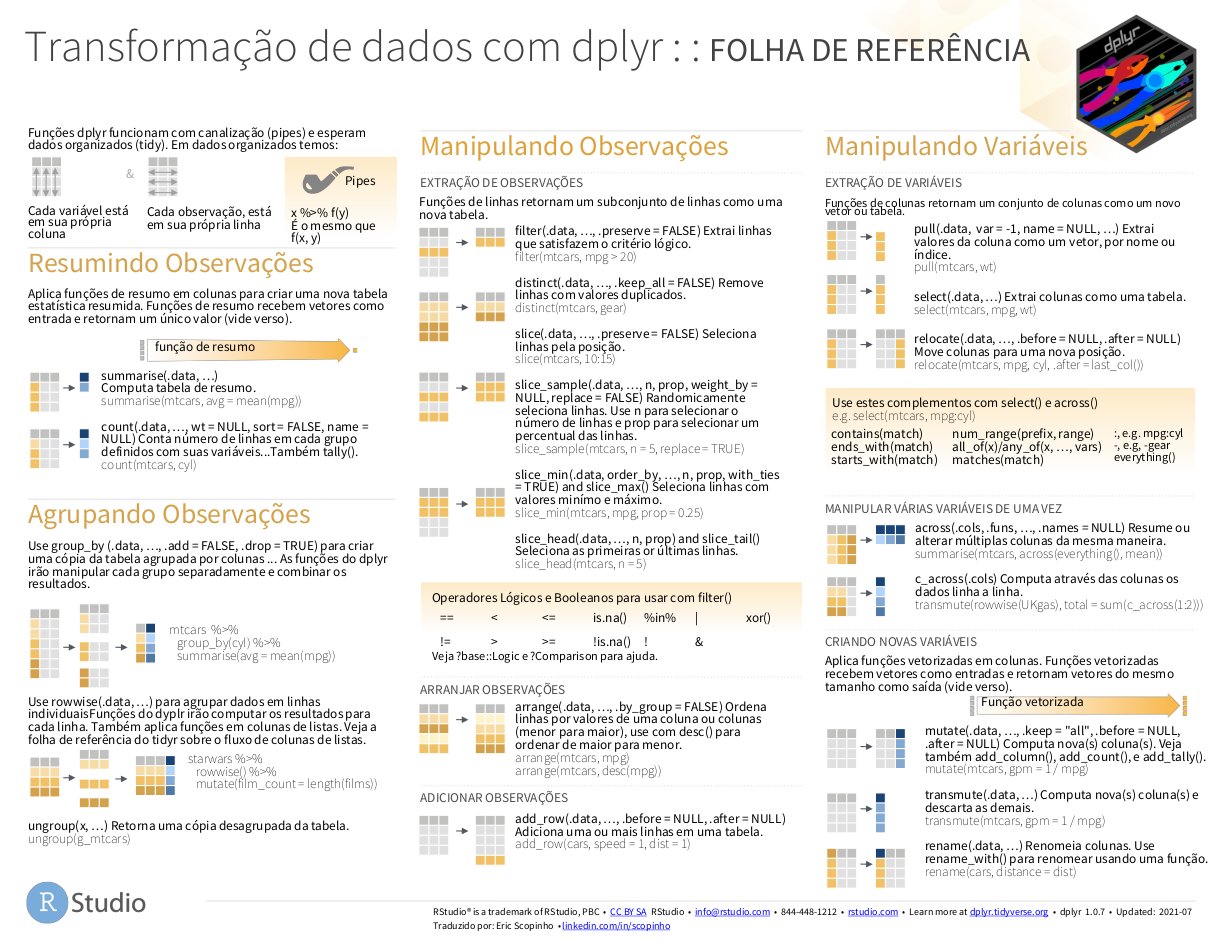
\includegraphics{Transformacao/images/cs-dplyr-01.png}}

}

\end{figure}

\begin{figure}

{\centering 

\href{images/cs-dplyr-02.png}{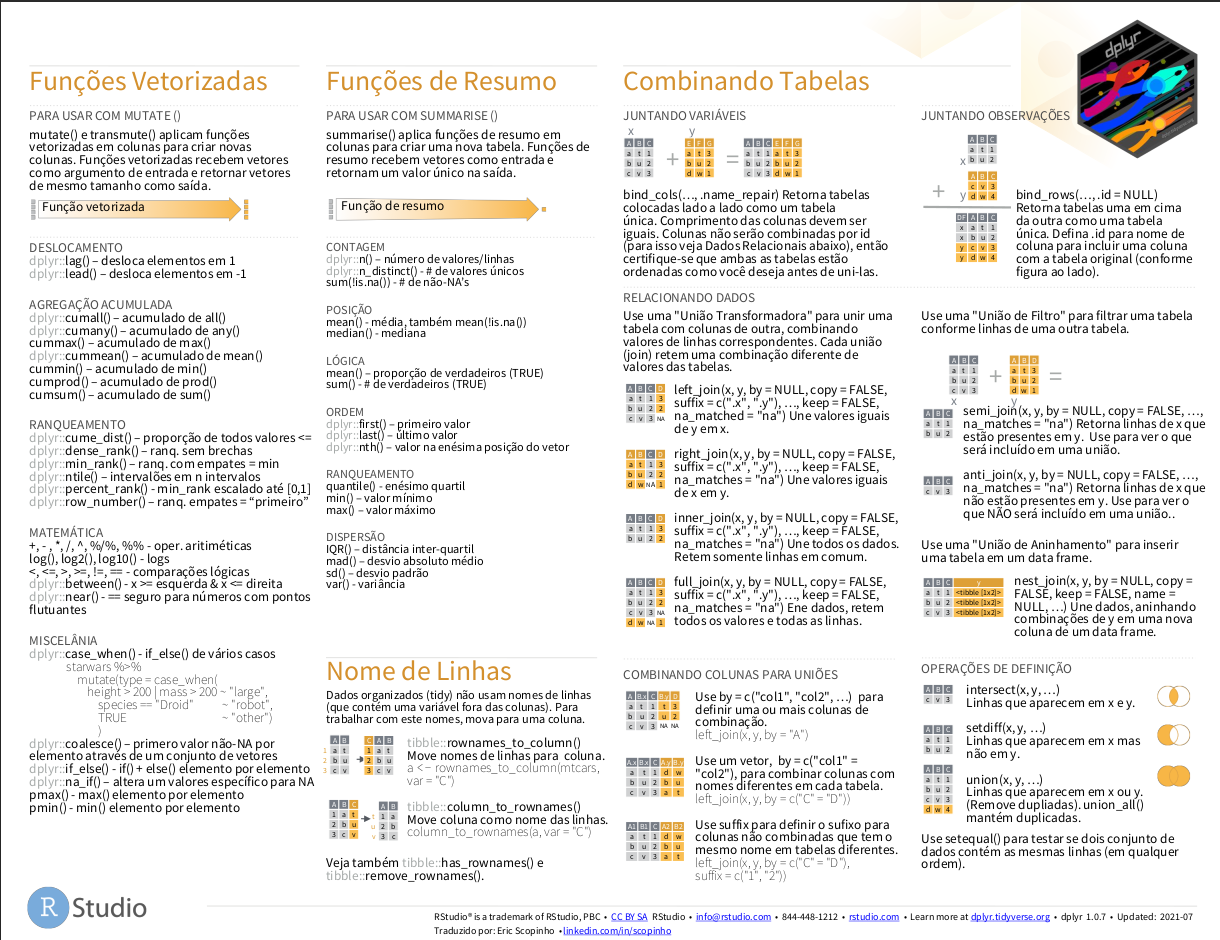
\includegraphics{Transformacao/images/cs-dplyr-02.png}}

}

\end{figure}

\hypertarget{base-de-dados}{%
\subsection{Base de Dados}\label{base-de-dados}}

Para a maioria dos exemplos utilizaremos as bases de dados
\textbf{mtcars} e \textbf{starwars} provenientes do pacote
\textbf{datasets e dplyr}.

\begin{tcolorbox}[enhanced jigsaw, rightrule=.15mm, arc=.35mm, coltitle=black, colframe=quarto-callout-note-color-frame, opacityback=0, toprule=.15mm, left=2mm, breakable, colback=white, bottomtitle=1mm, leftrule=.75mm, title=\textcolor{quarto-callout-note-color}{\faInfo}\hspace{0.5em}{Nota}, colbacktitle=quarto-callout-note-color!10!white, titlerule=0mm, bottomrule=.15mm, toptitle=1mm, opacitybacktitle=0.6]
\emph{Em alguns casos, onde o volume de dados de saída pode ser extenso,
usamos também a função \textbf{head()} para mostrar apenas as linhas
iniciais. Quando o exemplo possui muitas colunas de saída, eventualmente
utilizamos a função \textbf{select()} do pacote dplyr para selecionar
apenas algumas colunas.}
\end{tcolorbox}

\begin{center}\rule{0.5\linewidth}{0.5pt}\end{center}

\textbf{MTCARS}: Dados de consumo de combustível, performance e design
de 32 automóveis ( \emph{1974 Motor Trend US magazine})

\begin{Shaded}
\begin{Highlighting}[]
\NormalTok{mtcars }
\end{Highlighting}
\end{Shaded}

\begin{verbatim}
                     mpg cyl  disp  hp drat    wt  qsec vs am gear carb
Mazda RX4           21.0   6 160.0 110 3.90 2.620 16.46  0  1    4    4
Mazda RX4 Wag       21.0   6 160.0 110 3.90 2.875 17.02  0  1    4    4
Datsun 710          22.8   4 108.0  93 3.85 2.320 18.61  1  1    4    1
Hornet 4 Drive      21.4   6 258.0 110 3.08 3.215 19.44  1  0    3    1
Hornet Sportabout   18.7   8 360.0 175 3.15 3.440 17.02  0  0    3    2
Valiant             18.1   6 225.0 105 2.76 3.460 20.22  1  0    3    1
Duster 360          14.3   8 360.0 245 3.21 3.570 15.84  0  0    3    4
Merc 240D           24.4   4 146.7  62 3.69 3.190 20.00  1  0    4    2
Merc 230            22.8   4 140.8  95 3.92 3.150 22.90  1  0    4    2
Merc 280            19.2   6 167.6 123 3.92 3.440 18.30  1  0    4    4
Merc 280C           17.8   6 167.6 123 3.92 3.440 18.90  1  0    4    4
Merc 450SE          16.4   8 275.8 180 3.07 4.070 17.40  0  0    3    3
Merc 450SL          17.3   8 275.8 180 3.07 3.730 17.60  0  0    3    3
Merc 450SLC         15.2   8 275.8 180 3.07 3.780 18.00  0  0    3    3
Cadillac Fleetwood  10.4   8 472.0 205 2.93 5.250 17.98  0  0    3    4
Lincoln Continental 10.4   8 460.0 215 3.00 5.424 17.82  0  0    3    4
Chrysler Imperial   14.7   8 440.0 230 3.23 5.345 17.42  0  0    3    4
Fiat 128            32.4   4  78.7  66 4.08 2.200 19.47  1  1    4    1
Honda Civic         30.4   4  75.7  52 4.93 1.615 18.52  1  1    4    2
Toyota Corolla      33.9   4  71.1  65 4.22 1.835 19.90  1  1    4    1
Toyota Corona       21.5   4 120.1  97 3.70 2.465 20.01  1  0    3    1
Dodge Challenger    15.5   8 318.0 150 2.76 3.520 16.87  0  0    3    2
AMC Javelin         15.2   8 304.0 150 3.15 3.435 17.30  0  0    3    2
Camaro Z28          13.3   8 350.0 245 3.73 3.840 15.41  0  0    3    4
Pontiac Firebird    19.2   8 400.0 175 3.08 3.845 17.05  0  0    3    2
Fiat X1-9           27.3   4  79.0  66 4.08 1.935 18.90  1  1    4    1
Porsche 914-2       26.0   4 120.3  91 4.43 2.140 16.70  0  1    5    2
Lotus Europa        30.4   4  95.1 113 3.77 1.513 16.90  1  1    5    2
Ford Pantera L      15.8   8 351.0 264 4.22 3.170 14.50  0  1    5    4
Ferrari Dino        19.7   6 145.0 175 3.62 2.770 15.50  0  1    5    6
Maserati Bora       15.0   8 301.0 335 3.54 3.570 14.60  0  1    5    8
Volvo 142E          21.4   4 121.0 109 4.11 2.780 18.60  1  1    4    2
\end{verbatim}

\begin{center}\rule{0.5\linewidth}{0.5pt}\end{center}

\textbf{STARWARS}: Dados dos personagens de STAR WARS

\begin{Shaded}
\begin{Highlighting}[]
\NormalTok{starwars }
\end{Highlighting}
\end{Shaded}

\begin{verbatim}
# A tibble: 87 x 14
   name        height  mass hair_~1 skin_~2 eye_c~3 birth~4 sex   gender homew~5
   <chr>        <int> <dbl> <chr>   <chr>   <chr>     <dbl> <chr> <chr>  <chr>  
 1 Luke Skywa~    172    77 blond   fair    blue       19   male  mascu~ Tatooi~
 2 C-3PO          167    75 <NA>    gold    yellow    112   none  mascu~ Tatooi~
 3 R2-D2           96    32 <NA>    white,~ red        33   none  mascu~ Naboo  
 4 Darth Vader    202   136 none    white   yellow     41.9 male  mascu~ Tatooi~
 5 Leia Organa    150    49 brown   light   brown      19   fema~ femin~ Aldera~
 6 Owen Lars      178   120 brown,~ light   blue       52   male  mascu~ Tatooi~
 7 Beru White~    165    75 brown   light   blue       47   fema~ femin~ Tatooi~
 8 R5-D4           97    32 <NA>    white,~ red        NA   none  mascu~ Tatooi~
 9 Biggs Dark~    183    84 black   light   brown      24   male  mascu~ Tatooi~
10 Obi-Wan Ke~    182    77 auburn~ fair    blue-g~    57   male  mascu~ Stewjon
# ... with 77 more rows, 4 more variables: species <chr>, films <list>,
#   vehicles <list>, starships <list>, and abbreviated variable names
#   1: hair_color, 2: skin_color, 3: eye_color, 4: birth_year, 5: homeworld
# i Use `print(n = ...)` to see more rows, and `colnames()` to see all variable names
\end{verbatim}

\begin{tcolorbox}[enhanced jigsaw, rightrule=.15mm, arc=.35mm, coltitle=black, colframe=quarto-callout-note-color-frame, opacityback=0, toprule=.15mm, left=2mm, breakable, colback=white, bottomtitle=1mm, leftrule=.75mm, title=\textcolor{quarto-callout-note-color}{\faInfo}\hspace{0.5em}{Nota}, colbacktitle=quarto-callout-note-color!10!white, titlerule=0mm, bottomrule=.15mm, toptitle=1mm, opacitybacktitle=0.6]
\emph{O termo \uline{data-frame} descrito ao longo deste texto, é
utilizado de forma livre para objetos do tipo data.frame, tibble, entre
outros. Pense como se fosse uma tabela de um banco de dados e/ou uma
planilha do MS Excel, contendo linhas e colunas. Apesar de não ser
rigorosamente igual à uma tabela, muitas vezes usaremos estes termos de
forma intercambiável para facilitar o entendimento de iniciantes.}
\end{tcolorbox}

\hypertarget{dados-organizados-e-canalizauxe7uxe3o}{%
\subsection{Dados Organizados e
Canalização}\label{dados-organizados-e-canalizauxe7uxe3o}}

Relembrando o que visto anteriormente, dados organizados (\emph{tidy})
são estruturados onde:

Cada \textbf{variável} está em sua própria \textbf{coluna} e cada
\textbf{observação} está em sua própria \textbf{linha}.

\includegraphics{Transformacao/images/tidy_data01.png}

\textbf{Canalização} (\emph{Piping}) é uma forma de sequenciar as
funções, facilitando a leitura de várias funções em conjunto.

O símbolo \textbf{\textbar\textgreater{}} é utilizado para esta
finalidade.

\textbf{Exemplo}: x \textbar\textgreater{} f(y), é o mesmo que f(x,y)

\hypertarget{resumindo-observauxe7uxf5es}{%
\section{Resumindo Observações}\label{resumindo-observauxe7uxf5es}}

O pacote dplyr possui uma série de funções que nos permitem condesar
(resumir) os dados de uma tabela (data frame).

As \textbf{Funções de resumo} \textbf{recebem} \textbf{vetores} como
entrada e \textbf{retornam} um \textbf{único valor}. Vejamos algumas
delas:

\hypertarget{summarise}{%
\subsubsection{summarise}\label{summarise}}

\begin{Shaded}
\begin{Highlighting}[]
\FunctionTok{summarise}\NormalTok{ (mtcars, }\AttributeTok{media=}\FunctionTok{mean}\NormalTok{(mpg)) }
\end{Highlighting}
\end{Shaded}

\begin{verbatim}
     media
1 20.09062
\end{verbatim}

Cria um novo data-frame. Ele gera uma linha para cada combinação de
grupos de variáveis. Se não houver grupos, a saída será uma única linha
resumindo todas as observações da entrada.

No exemplo acima, não especificamos nenhum grupo (mais na seção
\protect\hyperlink{agrupando-observauxe7uxf5es}{Agrupando Observações}),
por isso, ele retorna apenas uma linha resumindo todas as observações de
mtcars. Como também especificamos a função de \textbf{mean(}), o valor
retornado será a média da coluna \textbf{mpg} para todas as observações
do data frame em uma única variável (coluna) chamada \textbf{média}.

Outra forma de se escrever o comando acima, utilizando a canalização
(``pinping'') descrita acima, seria:

\begin{Shaded}
\begin{Highlighting}[]
\NormalTok{mtcars }\SpecialCharTok{|\textgreater{}} 
  \FunctionTok{summarise}\NormalTok{(média }\OtherTok{=} \FunctionTok{mean}\NormalTok{(mpg))}
\end{Highlighting}
\end{Shaded}

Ver a seção de \protect\hyperlink{funuxe7uxf5es-de-resumo}{Funções de
Resumo} para mais detalhes.

\hypertarget{count}{%
\subsubsection{count}\label{count}}

Conta valores únicos de uma ou mais variáveis.

\begin{Shaded}
\begin{Highlighting}[]
\NormalTok{mtcars }\SpecialCharTok{|\textgreater{}} 
  \FunctionTok{count}\NormalTok{ (cyl) }
\end{Highlighting}
\end{Shaded}

\begin{verbatim}
  cyl  n
1   4 11
2   6  7
3   8 14
\end{verbatim}

No exemplo acima, contamos os valores únicos da variável \textbf{cyl} e
mostramos na variável \textbf{n}.

Um equivalente seria utilizar o \textbf{summarise} com o \textbf{grupo}
criado na variável cyl:

\begin{Shaded}
\begin{Highlighting}[]
\NormalTok{mtcars }\SpecialCharTok{|\textgreater{}} 
  \FunctionTok{group\_by}\NormalTok{(cyl) }\SpecialCharTok{|\textgreater{}} 
  \FunctionTok{summarise}\NormalTok{(}\AttributeTok{n =} \FunctionTok{n}\NormalTok{())}
\end{Highlighting}
\end{Shaded}

\begin{tcolorbox}[enhanced jigsaw, rightrule=.15mm, arc=.35mm, coltitle=black, colframe=quarto-callout-note-color-frame, opacityback=0, toprule=.15mm, left=2mm, breakable, colback=white, bottomtitle=1mm, leftrule=.75mm, title=\textcolor{quarto-callout-note-color}{\faInfo}\hspace{0.5em}{Nota}, colbacktitle=quarto-callout-note-color!10!white, titlerule=0mm, bottomrule=.15mm, toptitle=1mm, opacitybacktitle=0.6]
O pacote dyplr possui algumas ``\textbf{expressões de contexto}'' que
retornam informações sobre o \textbf{grupo} ou \textbf{variável
corrente}, mas só funcionam em contextos específicos como
\textbf{summarise}() ou \textbf{mutate}(). No caso acima, a função
\textbf{n()} é uma destas expressões, é por isso que criamos o grupo com
a função group\_by().

Mais sobre a função \textbf{group\_by} na seção
\protect\hyperlink{agrupando-observauxe7uxf5es}{Agrupando Observações}.
\end{tcolorbox}

\hypertarget{agrupando-observauxe7uxf5es}{%
\section{Agrupando Observações}\label{agrupando-observauxe7uxf5es}}

\hypertarget{group_by}{%
\subsubsection{group\_by}\label{group_by}}

Use \textbf{group\_by} (.data, \ldots, .add = FALSE, .drop = TRUE) para
criar uma cópia da tabela agrupada por colunas.

\begin{tcolorbox}[enhanced jigsaw, rightrule=.15mm, arc=.35mm, coltitle=black, colframe=quarto-callout-important-color-frame, opacityback=0, toprule=.15mm, left=2mm, breakable, colback=white, bottomtitle=1mm, leftrule=.75mm, title=\textcolor{quarto-callout-important-color}{\faExclamation}\hspace{0.5em}{Importante}, colbacktitle=quarto-callout-important-color!10!white, titlerule=0mm, bottomrule=.15mm, toptitle=1mm, opacitybacktitle=0.6]
As funções do dplyr irão \textbf{manipular} cada \textbf{grupo}
\textbf{separadamente} e \textbf{combinar} os \textbf{resultados}.
\end{tcolorbox}

\begin{tcolorbox}[enhanced jigsaw, rightrule=.15mm, arc=.35mm, coltitle=black, colframe=quarto-callout-important-color-frame, opacityback=0, toprule=.15mm, left=2mm, breakable, colback=white, bottomtitle=1mm, leftrule=.75mm, title=\textcolor{quarto-callout-important-color}{\faExclamation}\hspace{0.5em}{Importante}, colbacktitle=quarto-callout-important-color!10!white, titlerule=0mm, bottomrule=.15mm, toptitle=1mm, opacitybacktitle=0.6]
Se compararmos o resultado de uma tabela antes e depois do agrupamento
(group\_by), apenas uma informação sobre o grupo será visível.

Isto significa que o agrupamento só afetará o resultado de saída se
utilizado em conjunto com funções que entendam esta mudança de contexto,
como as funções do dyplr.
\end{tcolorbox}

Por exemplo, \textbf{ANTES} de agruparmos pela variável \textbf{cyl}
(group\_by(cyl)) temos:

\begin{Shaded}
\begin{Highlighting}[]
\NormalTok{mtcars }\SpecialCharTok{|\textgreater{}} 
  \FunctionTok{as\_tibble}\NormalTok{() }\SpecialCharTok{|\textgreater{}} \FunctionTok{glimpse}\NormalTok{()}
\end{Highlighting}
\end{Shaded}

\begin{verbatim}
Rows: 32
Columns: 11
$ mpg  <dbl> 21.0, 21.0, 22.8, 21.4, 18.7, 18.1, 14.3, 24.4, 22.8, 19.2, 17.8,~
$ cyl  <dbl> 6, 6, 4, 6, 8, 6, 8, 4, 4, 6, 6, 8, 8, 8, 8, 8, 8, 4, 4, 4, 4, 8,~
$ disp <dbl> 160.0, 160.0, 108.0, 258.0, 360.0, 225.0, 360.0, 146.7, 140.8, 16~
$ hp   <dbl> 110, 110, 93, 110, 175, 105, 245, 62, 95, 123, 123, 180, 180, 180~
$ drat <dbl> 3.90, 3.90, 3.85, 3.08, 3.15, 2.76, 3.21, 3.69, 3.92, 3.92, 3.92,~
$ wt   <dbl> 2.620, 2.875, 2.320, 3.215, 3.440, 3.460, 3.570, 3.190, 3.150, 3.~
$ qsec <dbl> 16.46, 17.02, 18.61, 19.44, 17.02, 20.22, 15.84, 20.00, 22.90, 18~
$ vs   <dbl> 0, 0, 1, 1, 0, 1, 0, 1, 1, 1, 1, 0, 0, 0, 0, 0, 0, 1, 1, 1, 1, 0,~
$ am   <dbl> 1, 1, 1, 0, 0, 0, 0, 0, 0, 0, 0, 0, 0, 0, 0, 0, 0, 1, 1, 1, 0, 0,~
$ gear <dbl> 4, 4, 4, 3, 3, 3, 3, 4, 4, 4, 4, 3, 3, 3, 3, 3, 3, 4, 4, 4, 3, 3,~
$ carb <dbl> 4, 4, 1, 1, 2, 1, 4, 2, 2, 4, 4, 3, 3, 3, 4, 4, 4, 1, 2, 1, 1, 2,~
\end{verbatim}

\textbf{DEPOIS} do group\_by:

\begin{Shaded}
\begin{Highlighting}[]
\NormalTok{mtcars }\SpecialCharTok{|\textgreater{}} 
  \FunctionTok{group\_by}\NormalTok{(cyl) }\SpecialCharTok{|\textgreater{}} \FunctionTok{glimpse}\NormalTok{()}
\end{Highlighting}
\end{Shaded}

\begin{verbatim}
Rows: 32
Columns: 11
Groups: cyl [3]
$ mpg  <dbl> 21.0, 21.0, 22.8, 21.4, 18.7, 18.1, 14.3, 24.4, 22.8, 19.2, 17.8,~
$ cyl  <dbl> 6, 6, 4, 6, 8, 6, 8, 4, 4, 6, 6, 8, 8, 8, 8, 8, 8, 4, 4, 4, 4, 8,~
$ disp <dbl> 160.0, 160.0, 108.0, 258.0, 360.0, 225.0, 360.0, 146.7, 140.8, 16~
$ hp   <dbl> 110, 110, 93, 110, 175, 105, 245, 62, 95, 123, 123, 180, 180, 180~
$ drat <dbl> 3.90, 3.90, 3.85, 3.08, 3.15, 2.76, 3.21, 3.69, 3.92, 3.92, 3.92,~
$ wt   <dbl> 2.620, 2.875, 2.320, 3.215, 3.440, 3.460, 3.570, 3.190, 3.150, 3.~
$ qsec <dbl> 16.46, 17.02, 18.61, 19.44, 17.02, 20.22, 15.84, 20.00, 22.90, 18~
$ vs   <dbl> 0, 0, 1, 1, 0, 1, 0, 1, 1, 1, 1, 0, 0, 0, 0, 0, 0, 1, 1, 1, 1, 0,~
$ am   <dbl> 1, 1, 1, 0, 0, 0, 0, 0, 0, 0, 0, 0, 0, 0, 0, 0, 0, 1, 1, 1, 0, 0,~
$ gear <dbl> 4, 4, 4, 3, 3, 3, 3, 4, 4, 4, 4, 3, 3, 3, 3, 3, 3, 4, 4, 4, 3, 3,~
$ carb <dbl> 4, 4, 1, 1, 2, 1, 4, 2, 2, 4, 4, 3, 3, 3, 4, 4, 4, 1, 2, 1, 1, 2,~
\end{verbatim}

Veja que, exceto pela informação :

\textbf{'\# Groups: cyl {[}3{]}}

Todo o restante da saída é o mesmo. Por isso, é importante que
utilizemos o contexto do grupo, junto com outra função.

\textbf{Exemplo}: Se quiser criar uma tabela com a função
\textbf{summarise()} com apenas o grupo de cilindradas, podemos usar:

\begin{Shaded}
\begin{Highlighting}[]
\NormalTok{mtcars }\SpecialCharTok{|\textgreater{}} 
  \FunctionTok{group\_by}\NormalTok{(cyl) }\SpecialCharTok{|\textgreater{}} 
  \FunctionTok{summarise}\NormalTok{() }
\end{Highlighting}
\end{Shaded}

\begin{verbatim}
# A tibble: 3 x 1
    cyl
  <dbl>
1     4
2     6
3     8
\end{verbatim}

Supondo que quiséssemos agora, saber o número de carros, agrupados pela
variável cyl, podemos utilizar a função summarise, após o agrupamento,
criando uma coluna através da função de contexto \textbf{n()}.

\begin{Shaded}
\begin{Highlighting}[]
\NormalTok{mtcars }\SpecialCharTok{|\textgreater{}} 
  \FunctionTok{group\_by}\NormalTok{(cyl) }\SpecialCharTok{|\textgreater{}} 
  \FunctionTok{summarise}\NormalTok{(}\AttributeTok{num\_automoveis =} \FunctionTok{n}\NormalTok{()) }
\end{Highlighting}
\end{Shaded}

\begin{verbatim}
# A tibble: 3 x 2
    cyl num_automoveis
  <dbl>          <int>
1     4             11
2     6              7
3     8             14
\end{verbatim}

Em outro exemplo, podemos extrair o consumo médio (miles/gallon) dos
veículos agrupado pelo número de cilindros destes veículos.

\begin{Shaded}
\begin{Highlighting}[]
\NormalTok{mtcars }\SpecialCharTok{|\textgreater{}} 
  \FunctionTok{group\_by}\NormalTok{(cyl) }\SpecialCharTok{|\textgreater{}} 
  \FunctionTok{summarise}\NormalTok{(}\AttributeTok{consumo\_medio =} \FunctionTok{mean}\NormalTok{(mpg)) }
\end{Highlighting}
\end{Shaded}

\begin{verbatim}
# A tibble: 3 x 2
    cyl consumo_medio
  <dbl>         <dbl>
1     4          26.7
2     6          19.7
3     8          15.1
\end{verbatim}

O agrupamento pode ser feito para mais de uma variável também. Por
exemplo, se quisermos obter o consumo médio (miles/gallon) dos veículos
agrupado pelo número de cilindros destes veículos e também pelo número
de marchas, podemos ter:

\begin{tcolorbox}[enhanced jigsaw, rightrule=.15mm, arc=.35mm, coltitle=black, colframe=quarto-callout-note-color-frame, opacityback=0, toprule=.15mm, left=2mm, breakable, colback=white, bottomtitle=1mm, leftrule=.75mm, title=\textcolor{quarto-callout-note-color}{\faInfo}\hspace{0.5em}{Nota}, colbacktitle=quarto-callout-note-color!10!white, titlerule=0mm, bottomrule=.15mm, toptitle=1mm, opacitybacktitle=0.6]
A saída da função summarise, dependendo do caso, irá ser agrupada também
automaticamente, se quiser que isto não aconteça, utiliza a opção
\textbf{.groups=``drop''}.
\end{tcolorbox}

\begin{Shaded}
\begin{Highlighting}[]
\NormalTok{mtcars }\SpecialCharTok{|\textgreater{}} 
  \FunctionTok{group\_by}\NormalTok{(cyl, gear) }\SpecialCharTok{|\textgreater{}} 
  \FunctionTok{summarise}\NormalTok{(consumo\_médio }\OtherTok{=} \FunctionTok{mean}\NormalTok{(mpg), }\AttributeTok{.groups =} \StringTok{"drop"}\NormalTok{) }
\end{Highlighting}
\end{Shaded}

\begin{verbatim}
# A tibble: 8 x 3
    cyl  gear consumo_médio
  <dbl> <dbl>         <dbl>
1     4     3          21.5
2     4     4          26.9
3     4     5          28.2
4     6     3          19.8
5     6     4          19.8
6     6     5          19.7
7     8     3          15.0
8     8     5          15.4
\end{verbatim}

A função \textbf{un\_group()} remove os grupos definidos em uma tabela.
É uma boa prática, remover os grupos após efetuar uma sumarização, por
exemplo, afim de evitar resultados indesejáveis em sumarizações futuras.
Por exemplo:

\begin{Shaded}
\begin{Highlighting}[]
\NormalTok{mtcars }\SpecialCharTok{|\textgreater{}} 
  \FunctionTok{group\_by}\NormalTok{(cyl, gear) }\SpecialCharTok{|\textgreater{}} 
  \FunctionTok{summarise}\NormalTok{(}\AttributeTok{numero\_marchas =} \FunctionTok{n}\NormalTok{()) }\SpecialCharTok{|\textgreater{}} 
  \FunctionTok{ungroup}\NormalTok{() }
\end{Highlighting}
\end{Shaded}

\begin{verbatim}
# A tibble: 8 x 3
    cyl  gear numero_marchas
  <dbl> <dbl>          <int>
1     4     3              1
2     4     4              8
3     4     5              2
4     6     3              2
5     6     4              4
6     6     5              1
7     8     3             12
8     8     5              2
\end{verbatim}

No caso acima, se não tivessemos utilizado o desagrupamento
(\textbf{un\_group}), o resultado ainda teria os grupos demarcados.

\hypertarget{rowwise}{%
\subsubsection{rowwise}\label{rowwise}}

Use rowwise(.data, \ldots) para agrupar dados em linhas individuais.
Funções do dyplr irão computar os resultados para cada linha.

No exemplo abaixo, a tabela de dados \textbf{startwars}, possui uma
variável (\textbf{films}) que é o tipo lista, ou seja, a coluna contém
uma lista de filmes para cada personagem (observação).

Supondo que quiséssemos saber em quantos filmes cada personagem aparece:

\begin{Shaded}
\begin{Highlighting}[]
\NormalTok{starwars }\SpecialCharTok{|\textgreater{}} 
  \FunctionTok{select}\NormalTok{(name, films) }\SpecialCharTok{|\textgreater{}}
  \FunctionTok{rowwise}\NormalTok{() }\SpecialCharTok{|\textgreater{}}
  \FunctionTok{mutate}\NormalTok{(}\AttributeTok{quantos\_filmes =} \FunctionTok{length}\NormalTok{(films))}
\end{Highlighting}
\end{Shaded}

\begin{verbatim}
# A tibble: 87 x 3
# Rowwise: 
   name               films     quantos_filmes
   <chr>              <list>             <int>
 1 Luke Skywalker     <chr [5]>              5
 2 C-3PO              <chr [6]>              6
 3 R2-D2              <chr [7]>              7
 4 Darth Vader        <chr [4]>              4
 5 Leia Organa        <chr [5]>              5
 6 Owen Lars          <chr [3]>              3
 7 Beru Whitesun lars <chr [3]>              3
 8 R5-D4              <chr [1]>              1
 9 Biggs Darklighter  <chr [1]>              1
10 Obi-Wan Kenobi     <chr [6]>              6
# ... with 77 more rows
# i Use `print(n = ...)` to see more rows
\end{verbatim}

Em geral, utilizamos a função \textbf{rowwise} quando \uline{não temos
uma função vetorizada}, isto é, que não retorna um vetor e precisamos
aplicá-la em cada linha da tabela.

Veja a seção de \protect\hyperlink{funuxe7uxf5es-vetorizadas}{Funções
Vetorizadas}para maiores informações.

\hypertarget{manipulando-observauxe7uxf5es}{%
\section{Manipulando Observações}\label{manipulando-observauxe7uxf5es}}

\hypertarget{extrauxe7uxe3o-de-observauxe7uxf5es}{%
\subsection{Extração de
Observações}\label{extrauxe7uxe3o-de-observauxe7uxf5es}}

O dplyr possui uma série de funções que nos ajudam a extrair observações
(linhas) de uma tabela, dentre estas, temos:

\hypertarget{filter}{%
\subsubsection{filter}\label{filter}}

Extrai linhas de uma tablea que satisfazem o critério lógico.

filter(.data, \ldots, .preserve = FALSE)

\textbf{Exemplo}: Para extrair apenas os veículos que possuem consumo
(miles/galon) acima de 20, podemos usar:

\begin{Shaded}
\begin{Highlighting}[]
\FunctionTok{filter}\NormalTok{(mtcars, mpg }\SpecialCharTok{\textgreater{}} \DecValTok{20}\NormalTok{) }
\end{Highlighting}
\end{Shaded}

\begin{verbatim}
                mpg cyl  disp  hp drat    wt  qsec vs am gear carb
Mazda RX4      21.0   6 160.0 110 3.90 2.620 16.46  0  1    4    4
Mazda RX4 Wag  21.0   6 160.0 110 3.90 2.875 17.02  0  1    4    4
Datsun 710     22.8   4 108.0  93 3.85 2.320 18.61  1  1    4    1
Hornet 4 Drive 21.4   6 258.0 110 3.08 3.215 19.44  1  0    3    1
Merc 240D      24.4   4 146.7  62 3.69 3.190 20.00  1  0    4    2
Merc 230       22.8   4 140.8  95 3.92 3.150 22.90  1  0    4    2
Fiat 128       32.4   4  78.7  66 4.08 2.200 19.47  1  1    4    1
Honda Civic    30.4   4  75.7  52 4.93 1.615 18.52  1  1    4    2
Toyota Corolla 33.9   4  71.1  65 4.22 1.835 19.90  1  1    4    1
Toyota Corona  21.5   4 120.1  97 3.70 2.465 20.01  1  0    3    1
Fiat X1-9      27.3   4  79.0  66 4.08 1.935 18.90  1  1    4    1
Porsche 914-2  26.0   4 120.3  91 4.43 2.140 16.70  0  1    5    2
Lotus Europa   30.4   4  95.1 113 3.77 1.513 16.90  1  1    5    2
Volvo 142E     21.4   4 121.0 109 4.11 2.780 18.60  1  1    4    2
\end{verbatim}

Podemos utilizar operadores lógicos para ajustar os critérios do filtro,
como por exemplo, os operadores abaixo:

\textbf{==, \textgreater, \textgreater=, \&, \textbar, !, xor(),
is.na(), between(), near()}, entre outros

Por exemplo, para filtrar os veículos com consumo acima de 20 \textbf{E}
com apenas 3 marchas, temos:

\begin{Shaded}
\begin{Highlighting}[]
\NormalTok{mtcars }\SpecialCharTok{|\textgreater{}} 
  \FunctionTok{filter}\NormalTok{(mpg }\SpecialCharTok{\textgreater{}} \DecValTok{20} \SpecialCharTok{\&}\NormalTok{ gear }\SpecialCharTok{==} \DecValTok{3}\NormalTok{) }
\end{Highlighting}
\end{Shaded}

\begin{verbatim}
                mpg cyl  disp  hp drat    wt  qsec vs am gear carb
Hornet 4 Drive 21.4   6 258.0 110 3.08 3.215 19.44  1  0    3    1
Toyota Corona  21.5   4 120.1  97 3.70 2.465 20.01  1  0    3    1
\end{verbatim}

\hypertarget{distinct}{%
\subsubsection{distinct}\label{distinct}}

Remove linhas com valores duplicados, retornando apenas os valores
únicos da variável (coluna).

distinct(.data, \ldots, .keep\_all = FALSE) .

Por exemplo, se precisarmos saber quais os valores da variável gear
(marcha), podemos utilizar:

\begin{Shaded}
\begin{Highlighting}[]
\NormalTok{mtcars }\SpecialCharTok{|\textgreater{}} 
  \FunctionTok{distinct}\NormalTok{(gear) }
\end{Highlighting}
\end{Shaded}

\begin{verbatim}
               gear
Mazda RX4         4
Hornet 4 Drive    3
Porsche 914-2     5
\end{verbatim}

\begin{tcolorbox}[enhanced jigsaw, rightrule=.15mm, arc=.35mm, coltitle=black, colframe=quarto-callout-note-color-frame, opacityback=0, toprule=.15mm, left=2mm, breakable, colback=white, bottomtitle=1mm, leftrule=.75mm, title=\textcolor{quarto-callout-note-color}{\faInfo}\hspace{0.5em}{Nota}, colbacktitle=quarto-callout-note-color!10!white, titlerule=0mm, bottomrule=.15mm, toptitle=1mm, opacitybacktitle=0.6]
Se utilizar o código acima, verá que o R possui um ``nome'' para as
linhas. É importante ressaltar que este nome NÃO é uma variável da
tabela, ou seja, não temos uma coluna com o ``nome'' do veículo, é por
isso que você vê nomes de veículos, mesmo pedindo os valores únicos das
marchas. Para maiores informações sobre isso, veja a seção
\protect\hyperlink{nome-de-linhas}{Nome de Linhas}.
\end{tcolorbox}

\hypertarget{slice}{%
\subsubsection{slice}\label{slice}}

Seleciona linhas pelas suas respectivas posições nda tabela.

slice(.data, \ldots, .preserve = FALSE)

Por exemplo, para selecionarmos apenas da linha 10 até a linha 15 da
tabela usamos:

\begin{Shaded}
\begin{Highlighting}[]
\NormalTok{ mtcars }\SpecialCharTok{|\textgreater{}} 
   \FunctionTok{slice}\NormalTok{(}\DecValTok{10}\SpecialCharTok{:}\DecValTok{15}\NormalTok{) }
\end{Highlighting}
\end{Shaded}

\begin{verbatim}
                    mpg cyl  disp  hp drat   wt  qsec vs am gear carb
Merc 280           19.2   6 167.6 123 3.92 3.44 18.30  1  0    4    4
Merc 280C          17.8   6 167.6 123 3.92 3.44 18.90  1  0    4    4
Merc 450SE         16.4   8 275.8 180 3.07 4.07 17.40  0  0    3    3
Merc 450SL         17.3   8 275.8 180 3.07 3.73 17.60  0  0    3    3
Merc 450SLC        15.2   8 275.8 180 3.07 3.78 18.00  0  0    3    3
Cadillac Fleetwood 10.4   8 472.0 205 2.93 5.25 17.98  0  0    3    4
\end{verbatim}

Veja que em alguns casos, podemos utilizar um equivalente filtro para
obter o mesmo resultado:

\begin{Shaded}
\begin{Highlighting}[]
\NormalTok{mtcars }\SpecialCharTok{|\textgreater{}} 
  \FunctionTok{filter}\NormalTok{(}\FunctionTok{between}\NormalTok{(}\FunctionTok{row\_number}\NormalTok{(), }\DecValTok{10}\NormalTok{, }\DecValTok{15}\NormalTok{)) }
\end{Highlighting}
\end{Shaded}

\begin{verbatim}
                    mpg cyl  disp  hp drat   wt  qsec vs am gear carb
Merc 280           19.2   6 167.6 123 3.92 3.44 18.30  1  0    4    4
Merc 280C          17.8   6 167.6 123 3.92 3.44 18.90  1  0    4    4
Merc 450SE         16.4   8 275.8 180 3.07 4.07 17.40  0  0    3    3
Merc 450SL         17.3   8 275.8 180 3.07 3.73 17.60  0  0    3    3
Merc 450SLC        15.2   8 275.8 180 3.07 3.78 18.00  0  0    3    3
Cadillac Fleetwood 10.4   8 472.0 205 2.93 5.25 17.98  0  0    3    4
\end{verbatim}

\hypertarget{slice_sample}{%
\subsubsection{slice\_sample}\label{slice_sample}}

Para randomicamente selecionar linhas da tabela. Use \textbf{n} para
selecionar o número de linhas ou \textbf{prop} para selecionar um
percentual das linhas.

slice\_sample(.data, \ldots, n, prop, weight\_by = NULL, replace =
FALSE) .

Para selecionar \textbf{5} linhas randomicas da tabela usamos:

\begin{Shaded}
\begin{Highlighting}[]
\NormalTok{mtcars }\SpecialCharTok{|\textgreater{}} 
  \FunctionTok{slice\_sample}\NormalTok{(}\AttributeTok{n =} \DecValTok{5}\NormalTok{, }\AttributeTok{replace =} \ConstantTok{TRUE}\NormalTok{) }
\end{Highlighting}
\end{Shaded}

\begin{verbatim}
                     mpg cyl disp  hp drat    wt  qsec vs am gear carb
Lincoln Continental 10.4   8  460 215 3.00 5.424 17.82  0  0    3    4
Datsun 710...2      22.8   4  108  93 3.85 2.320 18.61  1  1    4    1
Dodge Challenger    15.5   8  318 150 2.76 3.520 16.87  0  0    3    2
Hornet 4 Drive      21.4   6  258 110 3.08 3.215 19.44  1  0    3    1
Datsun 710...5      22.8   4  108  93 3.85 2.320 18.61  1  1    4    1
\end{verbatim}

Para selecionar \textbf{25\%} do total de linhas da tabela de forma
dandomica usamos:

\begin{Shaded}
\begin{Highlighting}[]
\NormalTok{mtcars }\SpecialCharTok{|\textgreater{}} 
  \FunctionTok{slice\_sample}\NormalTok{(}\AttributeTok{prop =} \FloatTok{0.25}\NormalTok{, }\AttributeTok{replace =} \ConstantTok{TRUE}\NormalTok{) }
\end{Highlighting}
\end{Shaded}

\begin{verbatim}
                   mpg cyl  disp  hp drat    wt  qsec vs am gear carb
Valiant...1       18.1   6 225.0 105 2.76 3.460 20.22  1  0    3    1
Honda Civic       30.4   4  75.7  52 4.93 1.615 18.52  1  1    4    2
Merc 280          19.2   6 167.6 123 3.92 3.440 18.30  1  0    4    4
Valiant...4       18.1   6 225.0 105 2.76 3.460 20.22  1  0    3    1
Hornet Sportabout 18.7   8 360.0 175 3.15 3.440 17.02  0  0    3    2
Fiat X1-9         27.3   4  79.0  66 4.08 1.935 18.90  1  1    4    1
Mazda RX4 Wag     21.0   6 160.0 110 3.90 2.875 17.02  0  1    4    4
Mazda RX4         21.0   6 160.0 110 3.90 2.620 16.46  0  1    4    4
\end{verbatim}

\hypertarget{slice_min}{%
\subsubsection{slice\_min}\label{slice_min}}

Seleciona linhas com valores minímo (slice\_min) ou máximo (slice\_max)
de uma variável.

slice\_min(.data, order\_by, \ldots, n, prop, with\_ties = TRUE) and
slice\_max() .

Por exemplo, com base no menor valor da variável de consumo do veículo
(mpg), retorne 25\% da tabela.

\begin{Shaded}
\begin{Highlighting}[]
\NormalTok{mtcars }\SpecialCharTok{|\textgreater{}} 
  \FunctionTok{slice\_min}\NormalTok{(mpg, }\AttributeTok{prop =} \FloatTok{0.25}\NormalTok{) }
\end{Highlighting}
\end{Shaded}

\begin{verbatim}
                     mpg cyl  disp  hp drat    wt  qsec vs am gear carb
Cadillac Fleetwood  10.4   8 472.0 205 2.93 5.250 17.98  0  0    3    4
Lincoln Continental 10.4   8 460.0 215 3.00 5.424 17.82  0  0    3    4
Camaro Z28          13.3   8 350.0 245 3.73 3.840 15.41  0  0    3    4
Duster 360          14.3   8 360.0 245 3.21 3.570 15.84  0  0    3    4
Chrysler Imperial   14.7   8 440.0 230 3.23 5.345 17.42  0  0    3    4
Maserati Bora       15.0   8 301.0 335 3.54 3.570 14.60  0  1    5    8
Merc 450SLC         15.2   8 275.8 180 3.07 3.780 18.00  0  0    3    3
AMC Javelin         15.2   8 304.0 150 3.15 3.435 17.30  0  0    3    2
\end{verbatim}

Outro exemplo, poderia ser que você precise retornar os 5 veículos de
maior consumo:

\begin{Shaded}
\begin{Highlighting}[]
\NormalTok{mtcars }\SpecialCharTok{|\textgreater{}} 
  \FunctionTok{slice\_max}\NormalTok{(mpg, }\AttributeTok{n =} \DecValTok{5}\NormalTok{) }
\end{Highlighting}
\end{Shaded}

\begin{verbatim}
                mpg cyl disp  hp drat    wt  qsec vs am gear carb
Toyota Corolla 33.9   4 71.1  65 4.22 1.835 19.90  1  1    4    1
Fiat 128       32.4   4 78.7  66 4.08 2.200 19.47  1  1    4    1
Honda Civic    30.4   4 75.7  52 4.93 1.615 18.52  1  1    4    2
Lotus Europa   30.4   4 95.1 113 3.77 1.513 16.90  1  1    5    2
Fiat X1-9      27.3   4 79.0  66 4.08 1.935 18.90  1  1    4    1
\end{verbatim}

\hypertarget{slice_head}{%
\subsubsection{slice\_head}\label{slice_head}}

Seleciona as primeiras (slice\_head) or últimas (slide\_tail) linhas de
uma tabela.

slice\_head(.data, \ldots, n, prop) and slice\_tail() .

Por exemplo, vamos selecionar as 5 primeiras linhas de mtcars:

\begin{Shaded}
\begin{Highlighting}[]
\NormalTok{mtcars }\SpecialCharTok{|\textgreater{}} 
  \FunctionTok{slice\_head}\NormalTok{(}\AttributeTok{n =} \DecValTok{5}\NormalTok{)}
\end{Highlighting}
\end{Shaded}

\begin{verbatim}
                   mpg cyl disp  hp drat    wt  qsec vs am gear carb
Mazda RX4         21.0   6  160 110 3.90 2.620 16.46  0  1    4    4
Mazda RX4 Wag     21.0   6  160 110 3.90 2.875 17.02  0  1    4    4
Datsun 710        22.8   4  108  93 3.85 2.320 18.61  1  1    4    1
Hornet 4 Drive    21.4   6  258 110 3.08 3.215 19.44  1  0    3    1
Hornet Sportabout 18.7   8  360 175 3.15 3.440 17.02  0  0    3    2
\end{verbatim}

\hypertarget{arranjar-observauxe7uxf5es}{%
\subsection{Arranjar Observações}\label{arranjar-observauxe7uxf5es}}

\hypertarget{arrange}{%
\subsubsection{arrange}\label{arrange}}

A função arrange ordena linhas por valores de uma coluna(s) (menor para
maior), use com a função \textbf{desc()} para ordenar de maior para
menor.

arrange(.data, \ldots, .by\_group = FALSE) arrange(mtcars, mpg) ou
arrange(mtcars, desc(mpg))

No exemplo abaixo, vamos ordenar a variável mpg, de forma a mostrar
primeiro os veículos com menor consumo de combustível até o de maior
consumo:

\begin{Shaded}
\begin{Highlighting}[]
\NormalTok{mtcars }\SpecialCharTok{|\textgreater{}} 
  \FunctionTok{arrange}\NormalTok{(mpg)}
\end{Highlighting}
\end{Shaded}

\begin{verbatim}
                     mpg cyl  disp  hp drat    wt  qsec vs am gear carb
Cadillac Fleetwood  10.4   8 472.0 205 2.93 5.250 17.98  0  0    3    4
Lincoln Continental 10.4   8 460.0 215 3.00 5.424 17.82  0  0    3    4
Camaro Z28          13.3   8 350.0 245 3.73 3.840 15.41  0  0    3    4
Duster 360          14.3   8 360.0 245 3.21 3.570 15.84  0  0    3    4
Chrysler Imperial   14.7   8 440.0 230 3.23 5.345 17.42  0  0    3    4
Maserati Bora       15.0   8 301.0 335 3.54 3.570 14.60  0  1    5    8
Merc 450SLC         15.2   8 275.8 180 3.07 3.780 18.00  0  0    3    3
AMC Javelin         15.2   8 304.0 150 3.15 3.435 17.30  0  0    3    2
Dodge Challenger    15.5   8 318.0 150 2.76 3.520 16.87  0  0    3    2
Ford Pantera L      15.8   8 351.0 264 4.22 3.170 14.50  0  1    5    4
Merc 450SE          16.4   8 275.8 180 3.07 4.070 17.40  0  0    3    3
Merc 450SL          17.3   8 275.8 180 3.07 3.730 17.60  0  0    3    3
Merc 280C           17.8   6 167.6 123 3.92 3.440 18.90  1  0    4    4
Valiant             18.1   6 225.0 105 2.76 3.460 20.22  1  0    3    1
Hornet Sportabout   18.7   8 360.0 175 3.15 3.440 17.02  0  0    3    2
Merc 280            19.2   6 167.6 123 3.92 3.440 18.30  1  0    4    4
Pontiac Firebird    19.2   8 400.0 175 3.08 3.845 17.05  0  0    3    2
Ferrari Dino        19.7   6 145.0 175 3.62 2.770 15.50  0  1    5    6
Mazda RX4           21.0   6 160.0 110 3.90 2.620 16.46  0  1    4    4
Mazda RX4 Wag       21.0   6 160.0 110 3.90 2.875 17.02  0  1    4    4
Hornet 4 Drive      21.4   6 258.0 110 3.08 3.215 19.44  1  0    3    1
Volvo 142E          21.4   4 121.0 109 4.11 2.780 18.60  1  1    4    2
Toyota Corona       21.5   4 120.1  97 3.70 2.465 20.01  1  0    3    1
Datsun 710          22.8   4 108.0  93 3.85 2.320 18.61  1  1    4    1
Merc 230            22.8   4 140.8  95 3.92 3.150 22.90  1  0    4    2
Merc 240D           24.4   4 146.7  62 3.69 3.190 20.00  1  0    4    2
Porsche 914-2       26.0   4 120.3  91 4.43 2.140 16.70  0  1    5    2
Fiat X1-9           27.3   4  79.0  66 4.08 1.935 18.90  1  1    4    1
Honda Civic         30.4   4  75.7  52 4.93 1.615 18.52  1  1    4    2
Lotus Europa        30.4   4  95.1 113 3.77 1.513 16.90  1  1    5    2
Fiat 128            32.4   4  78.7  66 4.08 2.200 19.47  1  1    4    1
Toyota Corolla      33.9   4  71.1  65 4.22 1.835 19.90  1  1    4    1
\end{verbatim}

\hypertarget{adicionar-observauxe7uxf5es}{%
\subsection{Adicionar Observações}\label{adicionar-observauxe7uxf5es}}

Algumas vezes precisamos adicionar observações (linhas) em uma tabela já
existente, neste caso podemos utilizar a função add\_row().

\hypertarget{add_row}{%
\subsubsection{add\_row}\label{add_row}}

add\_row(cars, speed = 1, dist = 1).

Neste caso, iremos adicionar uma nova linha na tables cars (não mtcars),
que possui apenas duas variáveis (speed e dist).

\begin{Shaded}
\begin{Highlighting}[]
\NormalTok{cars }\SpecialCharTok{|\textgreater{}} 
  \FunctionTok{add\_row}\NormalTok{(}\AttributeTok{speed =} \DecValTok{1}\NormalTok{, }\AttributeTok{dist =} \DecValTok{1}\NormalTok{) }\SpecialCharTok{|\textgreater{}} 
  \FunctionTok{tail}\NormalTok{() }
\end{Highlighting}
\end{Shaded}

\begin{verbatim}
   speed dist
46    24   70
47    24   92
48    24   93
49    24  120
50    25   85
51     1    1
\end{verbatim}

\hypertarget{manipulando-variuxe1veis}{%
\section{Manipulando Variáveis}\label{manipulando-variuxe1veis}}

\hypertarget{extrauxe7uxe3o-de-variuxe1veis}{%
\subsection{Extração de
Variáveis}\label{extrauxe7uxe3o-de-variuxe1veis}}

O dplyr possui uma série de funções que nos ajudam a obter um conjunto
de variáveis (colunas) como um novo vetor ou nova tabela:

\hypertarget{pull}{%
\subsubsection{pull}\label{pull}}

Extrai valores da coluna como um vetor, por nome ou índice.

pull(.data, var = -1, name = NULL, \ldots)

\begin{Shaded}
\begin{Highlighting}[]
\NormalTok{mtcars }\SpecialCharTok{|\textgreater{}} 
  \FunctionTok{pull}\NormalTok{ (wt) }
\end{Highlighting}
\end{Shaded}

\begin{verbatim}
 [1] 2.620 2.875 2.320 3.215 3.440 3.460 3.570 3.190 3.150 3.440 3.440 4.070
[13] 3.730 3.780 5.250 5.424 5.345 2.200 1.615 1.835 2.465 3.520 3.435 3.840
[25] 3.845 1.935 2.140 1.513 3.170 2.770 3.570 2.780
\end{verbatim}

No exemplo acima, a coluna peso (wt), é extraída da tabela e um obeto do
tipo vetor é retornado na saída.

Podemos extrair um vator de uma colunas também utilizando o número da
coluna. Se utilizarmos valores negativos, podemos extrair um vetor das
colunas contando a partir do lado direto.

Por exemplo, se quisermos extratir um vetor da penúltima coluna de uma
tabela, podemos usar:

\begin{Shaded}
\begin{Highlighting}[]
\NormalTok{mtcars }\SpecialCharTok{|\textgreater{}} 
  \FunctionTok{pull}\NormalTok{ (}\SpecialCharTok{{-}}\DecValTok{2}\NormalTok{)}
\end{Highlighting}
\end{Shaded}

\begin{verbatim}
 [1] 4 4 4 3 3 3 3 4 4 4 4 3 3 3 3 3 3 4 4 4 3 3 3 3 3 4 5 5 5 5 5 4
\end{verbatim}

\hypertarget{select}{%
\subsubsection{select}\label{select}}

Extrai valores de uma ou mais variáveis (colunas) e retorna uma nova
tabela, por nome ou índice.

select(.data, \ldots)

Por exemplo, podemos obter uma nova tabela contendo apenas as variáveis
mpg e wt usando:

\begin{Shaded}
\begin{Highlighting}[]
\NormalTok{mtcars }\SpecialCharTok{|\textgreater{}} 
  \FunctionTok{select}\NormalTok{ (mpg, wt) }
\end{Highlighting}
\end{Shaded}

\begin{verbatim}
                     mpg    wt
Mazda RX4           21.0 2.620
Mazda RX4 Wag       21.0 2.875
Datsun 710          22.8 2.320
Hornet 4 Drive      21.4 3.215
Hornet Sportabout   18.7 3.440
Valiant             18.1 3.460
Duster 360          14.3 3.570
Merc 240D           24.4 3.190
Merc 230            22.8 3.150
Merc 280            19.2 3.440
Merc 280C           17.8 3.440
Merc 450SE          16.4 4.070
Merc 450SL          17.3 3.730
Merc 450SLC         15.2 3.780
Cadillac Fleetwood  10.4 5.250
Lincoln Continental 10.4 5.424
Chrysler Imperial   14.7 5.345
Fiat 128            32.4 2.200
Honda Civic         30.4 1.615
Toyota Corolla      33.9 1.835
Toyota Corona       21.5 2.465
Dodge Challenger    15.5 3.520
AMC Javelin         15.2 3.435
Camaro Z28          13.3 3.840
Pontiac Firebird    19.2 3.845
Fiat X1-9           27.3 1.935
Porsche 914-2       26.0 2.140
Lotus Europa        30.4 1.513
Ford Pantera L      15.8 3.170
Ferrari Dino        19.7 2.770
Maserati Bora       15.0 3.570
Volvo 142E          21.4 2.780
\end{verbatim}

A função select possui um série de opções que tornam a seleção das
counas mais fáceis. A seguir temos algumas delas. Consulte a ajuda do
select usando ``?select'' para obter a lista completa.

\begin{itemize}
\item
  : para selecionar um range consecutivo de colunas
\item
  ! para pegar o complemento de uma conjunto de colunas
\item
  \& e \textbar{} para selecionar a intersecção ou união (E OU) de um
  conjunto de colunas
\item
  c() para combinar seleções
\end{itemize}

Além disso, possui também algumas funções que ajudam na seleção como:

\begin{itemize}
\tightlist
\item
  eveything(), last\_col(), starts\_with(), ends\_with(), contains(),
  matches(), num\_range()
\end{itemize}

Por exemplo, se quisermos selecionar toda a base mtcars, exceto as
colunas wt e mpg, podemos usar:

\begin{Shaded}
\begin{Highlighting}[]
\NormalTok{mtcars }\SpecialCharTok{|\textgreater{}} 
  \FunctionTok{select}\NormalTok{(}\SpecialCharTok{!}\FunctionTok{c}\NormalTok{(mpg, wt)) }
\end{Highlighting}
\end{Shaded}

\begin{verbatim}
                    cyl  disp  hp drat  qsec vs am gear carb
Mazda RX4             6 160.0 110 3.90 16.46  0  1    4    4
Mazda RX4 Wag         6 160.0 110 3.90 17.02  0  1    4    4
Datsun 710            4 108.0  93 3.85 18.61  1  1    4    1
Hornet 4 Drive        6 258.0 110 3.08 19.44  1  0    3    1
Hornet Sportabout     8 360.0 175 3.15 17.02  0  0    3    2
Valiant               6 225.0 105 2.76 20.22  1  0    3    1
Duster 360            8 360.0 245 3.21 15.84  0  0    3    4
Merc 240D             4 146.7  62 3.69 20.00  1  0    4    2
Merc 230              4 140.8  95 3.92 22.90  1  0    4    2
Merc 280              6 167.6 123 3.92 18.30  1  0    4    4
Merc 280C             6 167.6 123 3.92 18.90  1  0    4    4
Merc 450SE            8 275.8 180 3.07 17.40  0  0    3    3
Merc 450SL            8 275.8 180 3.07 17.60  0  0    3    3
Merc 450SLC           8 275.8 180 3.07 18.00  0  0    3    3
Cadillac Fleetwood    8 472.0 205 2.93 17.98  0  0    3    4
Lincoln Continental   8 460.0 215 3.00 17.82  0  0    3    4
Chrysler Imperial     8 440.0 230 3.23 17.42  0  0    3    4
Fiat 128              4  78.7  66 4.08 19.47  1  1    4    1
Honda Civic           4  75.7  52 4.93 18.52  1  1    4    2
Toyota Corolla        4  71.1  65 4.22 19.90  1  1    4    1
Toyota Corona         4 120.1  97 3.70 20.01  1  0    3    1
Dodge Challenger      8 318.0 150 2.76 16.87  0  0    3    2
AMC Javelin           8 304.0 150 3.15 17.30  0  0    3    2
Camaro Z28            8 350.0 245 3.73 15.41  0  0    3    4
Pontiac Firebird      8 400.0 175 3.08 17.05  0  0    3    2
Fiat X1-9             4  79.0  66 4.08 18.90  1  1    4    1
Porsche 914-2         4 120.3  91 4.43 16.70  0  1    5    2
Lotus Europa          4  95.1 113 3.77 16.90  1  1    5    2
Ford Pantera L        8 351.0 264 4.22 14.50  0  1    5    4
Ferrari Dino          6 145.0 175 3.62 15.50  0  1    5    6
Maserati Bora         8 301.0 335 3.54 14.60  0  1    5    8
Volvo 142E            4 121.0 109 4.11 18.60  1  1    4    2
\end{verbatim}

Se quisermos selecionar apenas as 4 primeiras colunas e também a coluna
wt, podemos usar:

\begin{Shaded}
\begin{Highlighting}[]
\NormalTok{mtcars }\SpecialCharTok{|\textgreater{}} 
  \FunctionTok{select}\NormalTok{ ((}\DecValTok{1}\SpecialCharTok{:}\DecValTok{4}\NormalTok{) }\SpecialCharTok{|}\NormalTok{ wt) }
\end{Highlighting}
\end{Shaded}

\begin{verbatim}
                     mpg cyl  disp  hp    wt
Mazda RX4           21.0   6 160.0 110 2.620
Mazda RX4 Wag       21.0   6 160.0 110 2.875
Datsun 710          22.8   4 108.0  93 2.320
Hornet 4 Drive      21.4   6 258.0 110 3.215
Hornet Sportabout   18.7   8 360.0 175 3.440
Valiant             18.1   6 225.0 105 3.460
Duster 360          14.3   8 360.0 245 3.570
Merc 240D           24.4   4 146.7  62 3.190
Merc 230            22.8   4 140.8  95 3.150
Merc 280            19.2   6 167.6 123 3.440
Merc 280C           17.8   6 167.6 123 3.440
Merc 450SE          16.4   8 275.8 180 4.070
Merc 450SL          17.3   8 275.8 180 3.730
Merc 450SLC         15.2   8 275.8 180 3.780
Cadillac Fleetwood  10.4   8 472.0 205 5.250
Lincoln Continental 10.4   8 460.0 215 5.424
Chrysler Imperial   14.7   8 440.0 230 5.345
Fiat 128            32.4   4  78.7  66 2.200
Honda Civic         30.4   4  75.7  52 1.615
Toyota Corolla      33.9   4  71.1  65 1.835
Toyota Corona       21.5   4 120.1  97 2.465
Dodge Challenger    15.5   8 318.0 150 3.520
AMC Javelin         15.2   8 304.0 150 3.435
Camaro Z28          13.3   8 350.0 245 3.840
Pontiac Firebird    19.2   8 400.0 175 3.845
Fiat X1-9           27.3   4  79.0  66 1.935
Porsche 914-2       26.0   4 120.3  91 2.140
Lotus Europa        30.4   4  95.1 113 1.513
Ford Pantera L      15.8   8 351.0 264 3.170
Ferrari Dino        19.7   6 145.0 175 2.770
Maserati Bora       15.0   8 301.0 335 3.570
Volvo 142E          21.4   4 121.0 109 2.780
\end{verbatim}

\hypertarget{relocate}{%
\subsubsection{relocate}\label{relocate}}

Move colunas para uma nova posição e retonar uma tabela com esta nova
order de colunas.

relocate(.data, \ldots, .before = NULL, .after = NULL)

\begin{Shaded}
\begin{Highlighting}[]
\NormalTok{mtcars }\SpecialCharTok{|\textgreater{}} 
  \FunctionTok{relocate}\NormalTok{ (mpg, cyl, }\AttributeTok{.after =} \FunctionTok{last\_col}\NormalTok{()) }
\end{Highlighting}
\end{Shaded}

\begin{verbatim}
                     disp  hp drat    wt  qsec vs am gear carb  mpg cyl
Mazda RX4           160.0 110 3.90 2.620 16.46  0  1    4    4 21.0   6
Mazda RX4 Wag       160.0 110 3.90 2.875 17.02  0  1    4    4 21.0   6
Datsun 710          108.0  93 3.85 2.320 18.61  1  1    4    1 22.8   4
Hornet 4 Drive      258.0 110 3.08 3.215 19.44  1  0    3    1 21.4   6
Hornet Sportabout   360.0 175 3.15 3.440 17.02  0  0    3    2 18.7   8
Valiant             225.0 105 2.76 3.460 20.22  1  0    3    1 18.1   6
Duster 360          360.0 245 3.21 3.570 15.84  0  0    3    4 14.3   8
Merc 240D           146.7  62 3.69 3.190 20.00  1  0    4    2 24.4   4
Merc 230            140.8  95 3.92 3.150 22.90  1  0    4    2 22.8   4
Merc 280            167.6 123 3.92 3.440 18.30  1  0    4    4 19.2   6
Merc 280C           167.6 123 3.92 3.440 18.90  1  0    4    4 17.8   6
Merc 450SE          275.8 180 3.07 4.070 17.40  0  0    3    3 16.4   8
Merc 450SL          275.8 180 3.07 3.730 17.60  0  0    3    3 17.3   8
Merc 450SLC         275.8 180 3.07 3.780 18.00  0  0    3    3 15.2   8
Cadillac Fleetwood  472.0 205 2.93 5.250 17.98  0  0    3    4 10.4   8
Lincoln Continental 460.0 215 3.00 5.424 17.82  0  0    3    4 10.4   8
Chrysler Imperial   440.0 230 3.23 5.345 17.42  0  0    3    4 14.7   8
Fiat 128             78.7  66 4.08 2.200 19.47  1  1    4    1 32.4   4
Honda Civic          75.7  52 4.93 1.615 18.52  1  1    4    2 30.4   4
Toyota Corolla       71.1  65 4.22 1.835 19.90  1  1    4    1 33.9   4
Toyota Corona       120.1  97 3.70 2.465 20.01  1  0    3    1 21.5   4
Dodge Challenger    318.0 150 2.76 3.520 16.87  0  0    3    2 15.5   8
AMC Javelin         304.0 150 3.15 3.435 17.30  0  0    3    2 15.2   8
Camaro Z28          350.0 245 3.73 3.840 15.41  0  0    3    4 13.3   8
Pontiac Firebird    400.0 175 3.08 3.845 17.05  0  0    3    2 19.2   8
Fiat X1-9            79.0  66 4.08 1.935 18.90  1  1    4    1 27.3   4
Porsche 914-2       120.3  91 4.43 2.140 16.70  0  1    5    2 26.0   4
Lotus Europa         95.1 113 3.77 1.513 16.90  1  1    5    2 30.4   4
Ford Pantera L      351.0 264 4.22 3.170 14.50  0  1    5    4 15.8   8
Ferrari Dino        145.0 175 3.62 2.770 15.50  0  1    5    6 19.7   6
Maserati Bora       301.0 335 3.54 3.570 14.60  0  1    5    8 15.0   8
Volvo 142E          121.0 109 4.11 2.780 18.60  1  1    4    2 21.4   4
\end{verbatim}

No exemplo acima, escolhermos mover as colunas mpg e cyl para depois (à
direita) da última coluna (last\_col()).

\hypertarget{manipular-vuxe1rias-variuxe1veis-de-uma-vez}{%
\subsection{Manipular Várias Variáveis de Uma
Vez}\label{manipular-vuxe1rias-variuxe1veis-de-uma-vez}}

Em algumas situações, desejamos manipular várias variáveis (colunas) de
uma só vez ou invés de cada coluna de cada vez. Para estes casos
,podemos usar as funções across e c\_across.

\hypertarget{across}{%
\subsubsection{across}\label{across}}

Resume ou alterar múltiplas colunas da mesma maneira. across(.cols,
.funs, \ldots, .names = NULL)

\begin{Shaded}
\begin{Highlighting}[]
\NormalTok{mtcars }\SpecialCharTok{|\textgreater{}} 
  \FunctionTok{summarise}\NormalTok{(}\FunctionTok{across}\NormalTok{(}\FunctionTok{everything}\NormalTok{(), mean)) }
\end{Highlighting}
\end{Shaded}

\begin{verbatim}
       mpg    cyl     disp       hp     drat      wt     qsec     vs      am
1 20.09062 6.1875 230.7219 146.6875 3.596563 3.21725 17.84875 0.4375 0.40625
    gear   carb
1 3.6875 2.8125
\end{verbatim}

No exemplo acima, varremos todas (everything) as colunas da tabela e
resumimos aplicando a função de média (mean) nestas colunas.

No exemplo a seguir, iremos ``varrer'' as colunas 5 até 7 e arredondar
seus valores com apenas um digito usando a função round().

\begin{Shaded}
\begin{Highlighting}[]
\NormalTok{mtcars }\SpecialCharTok{|\textgreater{}} 
  \FunctionTok{mutate}\NormalTok{(}\FunctionTok{across}\NormalTok{(}\DecValTok{5}\SpecialCharTok{:}\DecValTok{7}\NormalTok{, }\SpecialCharTok{\textasciitilde{}} \FunctionTok{round}\NormalTok{(.x, }\AttributeTok{digits =} \DecValTok{1}\NormalTok{) )) }
\end{Highlighting}
\end{Shaded}

\begin{verbatim}
                     mpg cyl  disp  hp drat  wt qsec vs am gear carb
Mazda RX4           21.0   6 160.0 110  3.9 2.6 16.5  0  1    4    4
Mazda RX4 Wag       21.0   6 160.0 110  3.9 2.9 17.0  0  1    4    4
Datsun 710          22.8   4 108.0  93  3.9 2.3 18.6  1  1    4    1
Hornet 4 Drive      21.4   6 258.0 110  3.1 3.2 19.4  1  0    3    1
Hornet Sportabout   18.7   8 360.0 175  3.1 3.4 17.0  0  0    3    2
Valiant             18.1   6 225.0 105  2.8 3.5 20.2  1  0    3    1
Duster 360          14.3   8 360.0 245  3.2 3.6 15.8  0  0    3    4
Merc 240D           24.4   4 146.7  62  3.7 3.2 20.0  1  0    4    2
Merc 230            22.8   4 140.8  95  3.9 3.1 22.9  1  0    4    2
Merc 280            19.2   6 167.6 123  3.9 3.4 18.3  1  0    4    4
Merc 280C           17.8   6 167.6 123  3.9 3.4 18.9  1  0    4    4
Merc 450SE          16.4   8 275.8 180  3.1 4.1 17.4  0  0    3    3
Merc 450SL          17.3   8 275.8 180  3.1 3.7 17.6  0  0    3    3
Merc 450SLC         15.2   8 275.8 180  3.1 3.8 18.0  0  0    3    3
Cadillac Fleetwood  10.4   8 472.0 205  2.9 5.2 18.0  0  0    3    4
Lincoln Continental 10.4   8 460.0 215  3.0 5.4 17.8  0  0    3    4
Chrysler Imperial   14.7   8 440.0 230  3.2 5.3 17.4  0  0    3    4
Fiat 128            32.4   4  78.7  66  4.1 2.2 19.5  1  1    4    1
Honda Civic         30.4   4  75.7  52  4.9 1.6 18.5  1  1    4    2
Toyota Corolla      33.9   4  71.1  65  4.2 1.8 19.9  1  1    4    1
Toyota Corona       21.5   4 120.1  97  3.7 2.5 20.0  1  0    3    1
Dodge Challenger    15.5   8 318.0 150  2.8 3.5 16.9  0  0    3    2
AMC Javelin         15.2   8 304.0 150  3.1 3.4 17.3  0  0    3    2
Camaro Z28          13.3   8 350.0 245  3.7 3.8 15.4  0  0    3    4
Pontiac Firebird    19.2   8 400.0 175  3.1 3.8 17.0  0  0    3    2
Fiat X1-9           27.3   4  79.0  66  4.1 1.9 18.9  1  1    4    1
Porsche 914-2       26.0   4 120.3  91  4.4 2.1 16.7  0  1    5    2
Lotus Europa        30.4   4  95.1 113  3.8 1.5 16.9  1  1    5    2
Ford Pantera L      15.8   8 351.0 264  4.2 3.2 14.5  0  1    5    4
Ferrari Dino        19.7   6 145.0 175  3.6 2.8 15.5  0  1    5    6
Maserati Bora       15.0   8 301.0 335  3.5 3.6 14.6  0  1    5    8
Volvo 142E          21.4   4 121.0 109  4.1 2.8 18.6  1  1    4    2
\end{verbatim}

\hypertarget{c_across}{%
\subsubsection{c\_across}\label{c_across}}

Computa através das colunas os dados linha a linha. Em geral, esta
função é utilizado em conjunto com a função rowwise().

c\_across(.cols)

\begin{Shaded}
\begin{Highlighting}[]
\NormalTok{mtcars }\SpecialCharTok{|\textgreater{}} 
  \FunctionTok{rowwise}\NormalTok{() }\SpecialCharTok{|\textgreater{}} 
  \FunctionTok{transmute}\NormalTok{ (}\AttributeTok{total =} \FunctionTok{sum}\NormalTok{(}\FunctionTok{c\_across}\NormalTok{(}\DecValTok{4}\SpecialCharTok{:}\DecValTok{6}\NormalTok{)))}
\end{Highlighting}
\end{Shaded}

\begin{verbatim}
# A tibble: 32 x 1
# Rowwise: 
   total
   <dbl>
 1 117. 
 2 117. 
 3  99.2
 4 116. 
 5 182. 
 6 111. 
 7 252. 
 8  68.9
 9 102. 
10 130. 
# ... with 22 more rows
# i Use `print(n = ...)` to see more rows
\end{verbatim}

No exemplo acima, ``varremos'' linha a linha da tabela e depois fazemos
a soma da coluna 4 até a coluna 6.

\hypertarget{criando-novas-variuxe1veis}{%
\subsection{Criando novas variáveis}\label{criando-novas-variuxe1veis}}

O dyplr possui a habilidade de criar novas variáveis (colunas) ou
alterar variáveis já existentes. Estes comandos, aplicam funções que são
de um tipo especial chamadas ``funções vetorizadas. Elas recebem vetores
como entradas e retornam vetores do mesmo tamanho como. Para maiores
detalhes veja a seção
\protect\hyperlink{funuxe7uxf5es-vetorizadas}{Funções Vetorizadas}.

\hypertarget{mutate}{%
\subsubsection{mutate}\label{mutate}}

Altera ou cria uma nova variável.

mutate(.data, \ldots, .keep = ``all'', .before = NULL, .after = NULL).

Por exemplo, se quisermos utilizar a variável \textbf{mpg} (milhas por
galão) e criar uma nova variável chamada \textbf{gpm} (galões por
milha), usamos:

\begin{Shaded}
\begin{Highlighting}[]
\NormalTok{mtcars }\SpecialCharTok{|\textgreater{}} 
  \FunctionTok{mutate}\NormalTok{ (}\AttributeTok{gpm =} \DecValTok{1} \SpecialCharTok{/}\NormalTok{ mpg) }
\end{Highlighting}
\end{Shaded}

\begin{verbatim}
                     mpg cyl  disp  hp drat    wt  qsec vs am gear carb
Mazda RX4           21.0   6 160.0 110 3.90 2.620 16.46  0  1    4    4
Mazda RX4 Wag       21.0   6 160.0 110 3.90 2.875 17.02  0  1    4    4
Datsun 710          22.8   4 108.0  93 3.85 2.320 18.61  1  1    4    1
Hornet 4 Drive      21.4   6 258.0 110 3.08 3.215 19.44  1  0    3    1
Hornet Sportabout   18.7   8 360.0 175 3.15 3.440 17.02  0  0    3    2
Valiant             18.1   6 225.0 105 2.76 3.460 20.22  1  0    3    1
Duster 360          14.3   8 360.0 245 3.21 3.570 15.84  0  0    3    4
Merc 240D           24.4   4 146.7  62 3.69 3.190 20.00  1  0    4    2
Merc 230            22.8   4 140.8  95 3.92 3.150 22.90  1  0    4    2
Merc 280            19.2   6 167.6 123 3.92 3.440 18.30  1  0    4    4
Merc 280C           17.8   6 167.6 123 3.92 3.440 18.90  1  0    4    4
Merc 450SE          16.4   8 275.8 180 3.07 4.070 17.40  0  0    3    3
Merc 450SL          17.3   8 275.8 180 3.07 3.730 17.60  0  0    3    3
Merc 450SLC         15.2   8 275.8 180 3.07 3.780 18.00  0  0    3    3
Cadillac Fleetwood  10.4   8 472.0 205 2.93 5.250 17.98  0  0    3    4
Lincoln Continental 10.4   8 460.0 215 3.00 5.424 17.82  0  0    3    4
Chrysler Imperial   14.7   8 440.0 230 3.23 5.345 17.42  0  0    3    4
Fiat 128            32.4   4  78.7  66 4.08 2.200 19.47  1  1    4    1
Honda Civic         30.4   4  75.7  52 4.93 1.615 18.52  1  1    4    2
Toyota Corolla      33.9   4  71.1  65 4.22 1.835 19.90  1  1    4    1
Toyota Corona       21.5   4 120.1  97 3.70 2.465 20.01  1  0    3    1
Dodge Challenger    15.5   8 318.0 150 2.76 3.520 16.87  0  0    3    2
AMC Javelin         15.2   8 304.0 150 3.15 3.435 17.30  0  0    3    2
Camaro Z28          13.3   8 350.0 245 3.73 3.840 15.41  0  0    3    4
Pontiac Firebird    19.2   8 400.0 175 3.08 3.845 17.05  0  0    3    2
Fiat X1-9           27.3   4  79.0  66 4.08 1.935 18.90  1  1    4    1
Porsche 914-2       26.0   4 120.3  91 4.43 2.140 16.70  0  1    5    2
Lotus Europa        30.4   4  95.1 113 3.77 1.513 16.90  1  1    5    2
Ford Pantera L      15.8   8 351.0 264 4.22 3.170 14.50  0  1    5    4
Ferrari Dino        19.7   6 145.0 175 3.62 2.770 15.50  0  1    5    6
Maserati Bora       15.0   8 301.0 335 3.54 3.570 14.60  0  1    5    8
Volvo 142E          21.4   4 121.0 109 4.11 2.780 18.60  1  1    4    2
                           gpm
Mazda RX4           0.04761905
Mazda RX4 Wag       0.04761905
Datsun 710          0.04385965
Hornet 4 Drive      0.04672897
Hornet Sportabout   0.05347594
Valiant             0.05524862
Duster 360          0.06993007
Merc 240D           0.04098361
Merc 230            0.04385965
Merc 280            0.05208333
Merc 280C           0.05617978
Merc 450SE          0.06097561
Merc 450SL          0.05780347
Merc 450SLC         0.06578947
Cadillac Fleetwood  0.09615385
Lincoln Continental 0.09615385
Chrysler Imperial   0.06802721
Fiat 128            0.03086420
Honda Civic         0.03289474
Toyota Corolla      0.02949853
Toyota Corona       0.04651163
Dodge Challenger    0.06451613
AMC Javelin         0.06578947
Camaro Z28          0.07518797
Pontiac Firebird    0.05208333
Fiat X1-9           0.03663004
Porsche 914-2       0.03846154
Lotus Europa        0.03289474
Ford Pantera L      0.06329114
Ferrari Dino        0.05076142
Maserati Bora       0.06666667
Volvo 142E          0.04672897
\end{verbatim}

\begin{tcolorbox}[enhanced jigsaw, rightrule=.15mm, arc=.35mm, coltitle=black, colframe=quarto-callout-caution-color-frame, opacityback=0, toprule=.15mm, left=2mm, breakable, colback=white, bottomtitle=1mm, leftrule=.75mm, title=\textcolor{quarto-callout-caution-color}{\faFire}\hspace{0.5em}{Cuidado}, colbacktitle=quarto-callout-caution-color!10!white, titlerule=0mm, bottomrule=.15mm, toptitle=1mm, opacitybacktitle=0.6]
É importante observar que a função mutate() considera o agrupamento da
tabela, caso houver. Em casos de funções de agregação e ranqueamento
(ex. média, ranque, etc), os valores de mutate serão considerados a
partir do agrupamento.
\end{tcolorbox}

Por exemplo, para criar uma coluna que mostra a diferença entre o
consumo do veículo e o consumo médio de todos os veículos, podemos usar:

\begin{Shaded}
\begin{Highlighting}[]
\NormalTok{mtcars }\SpecialCharTok{|\textgreater{}} 
  \FunctionTok{mutate}\NormalTok{ (}\AttributeTok{diferenca =}\NormalTok{ mpg }\SpecialCharTok{{-}} \FunctionTok{mean}\NormalTok{(mpg)) }
\end{Highlighting}
\end{Shaded}

\begin{verbatim}
                     mpg cyl  disp  hp drat    wt  qsec vs am gear carb
Mazda RX4           21.0   6 160.0 110 3.90 2.620 16.46  0  1    4    4
Mazda RX4 Wag       21.0   6 160.0 110 3.90 2.875 17.02  0  1    4    4
Datsun 710          22.8   4 108.0  93 3.85 2.320 18.61  1  1    4    1
Hornet 4 Drive      21.4   6 258.0 110 3.08 3.215 19.44  1  0    3    1
Hornet Sportabout   18.7   8 360.0 175 3.15 3.440 17.02  0  0    3    2
Valiant             18.1   6 225.0 105 2.76 3.460 20.22  1  0    3    1
Duster 360          14.3   8 360.0 245 3.21 3.570 15.84  0  0    3    4
Merc 240D           24.4   4 146.7  62 3.69 3.190 20.00  1  0    4    2
Merc 230            22.8   4 140.8  95 3.92 3.150 22.90  1  0    4    2
Merc 280            19.2   6 167.6 123 3.92 3.440 18.30  1  0    4    4
Merc 280C           17.8   6 167.6 123 3.92 3.440 18.90  1  0    4    4
Merc 450SE          16.4   8 275.8 180 3.07 4.070 17.40  0  0    3    3
Merc 450SL          17.3   8 275.8 180 3.07 3.730 17.60  0  0    3    3
Merc 450SLC         15.2   8 275.8 180 3.07 3.780 18.00  0  0    3    3
Cadillac Fleetwood  10.4   8 472.0 205 2.93 5.250 17.98  0  0    3    4
Lincoln Continental 10.4   8 460.0 215 3.00 5.424 17.82  0  0    3    4
Chrysler Imperial   14.7   8 440.0 230 3.23 5.345 17.42  0  0    3    4
Fiat 128            32.4   4  78.7  66 4.08 2.200 19.47  1  1    4    1
Honda Civic         30.4   4  75.7  52 4.93 1.615 18.52  1  1    4    2
Toyota Corolla      33.9   4  71.1  65 4.22 1.835 19.90  1  1    4    1
Toyota Corona       21.5   4 120.1  97 3.70 2.465 20.01  1  0    3    1
Dodge Challenger    15.5   8 318.0 150 2.76 3.520 16.87  0  0    3    2
AMC Javelin         15.2   8 304.0 150 3.15 3.435 17.30  0  0    3    2
Camaro Z28          13.3   8 350.0 245 3.73 3.840 15.41  0  0    3    4
Pontiac Firebird    19.2   8 400.0 175 3.08 3.845 17.05  0  0    3    2
Fiat X1-9           27.3   4  79.0  66 4.08 1.935 18.90  1  1    4    1
Porsche 914-2       26.0   4 120.3  91 4.43 2.140 16.70  0  1    5    2
Lotus Europa        30.4   4  95.1 113 3.77 1.513 16.90  1  1    5    2
Ford Pantera L      15.8   8 351.0 264 4.22 3.170 14.50  0  1    5    4
Ferrari Dino        19.7   6 145.0 175 3.62 2.770 15.50  0  1    5    6
Maserati Bora       15.0   8 301.0 335 3.54 3.570 14.60  0  1    5    8
Volvo 142E          21.4   4 121.0 109 4.11 2.780 18.60  1  1    4    2
                    diferenca
Mazda RX4            0.909375
Mazda RX4 Wag        0.909375
Datsun 710           2.709375
Hornet 4 Drive       1.309375
Hornet Sportabout   -1.390625
Valiant             -1.990625
Duster 360          -5.790625
Merc 240D            4.309375
Merc 230             2.709375
Merc 280            -0.890625
Merc 280C           -2.290625
Merc 450SE          -3.690625
Merc 450SL          -2.790625
Merc 450SLC         -4.890625
Cadillac Fleetwood  -9.690625
Lincoln Continental -9.690625
Chrysler Imperial   -5.390625
Fiat 128            12.309375
Honda Civic         10.309375
Toyota Corolla      13.809375
Toyota Corona        1.409375
Dodge Challenger    -4.590625
AMC Javelin         -4.890625
Camaro Z28          -6.790625
Pontiac Firebird    -0.890625
Fiat X1-9            7.209375
Porsche 914-2        5.909375
Lotus Europa        10.309375
Ford Pantera L      -4.290625
Ferrari Dino        -0.390625
Maserati Bora       -5.090625
Volvo 142E           1.309375
\end{verbatim}

Mas se quisermos saber a diferença de consumo com a média dos veículos
que possuem o mesmo número de cilindros, podemos fazer:

\begin{Shaded}
\begin{Highlighting}[]
\NormalTok{mtcars }\SpecialCharTok{|\textgreater{}} 
  \FunctionTok{group\_by}\NormalTok{(cyl) }\SpecialCharTok{|\textgreater{}} 
  \FunctionTok{mutate}\NormalTok{ (}\AttributeTok{diferenca =}\NormalTok{ mpg }\SpecialCharTok{{-}} \FunctionTok{mean}\NormalTok{(mpg)) }
\end{Highlighting}
\end{Shaded}

\begin{verbatim}
# A tibble: 32 x 12
# Groups:   cyl [3]
     mpg   cyl  disp    hp  drat    wt  qsec    vs    am  gear  carb diferenca
   <dbl> <dbl> <dbl> <dbl> <dbl> <dbl> <dbl> <dbl> <dbl> <dbl> <dbl>     <dbl>
 1  21       6  160    110  3.9   2.62  16.5     0     1     4     4     1.26 
 2  21       6  160    110  3.9   2.88  17.0     0     1     4     4     1.26 
 3  22.8     4  108     93  3.85  2.32  18.6     1     1     4     1    -3.86 
 4  21.4     6  258    110  3.08  3.22  19.4     1     0     3     1     1.66 
 5  18.7     8  360    175  3.15  3.44  17.0     0     0     3     2     3.6  
 6  18.1     6  225    105  2.76  3.46  20.2     1     0     3     1    -1.64 
 7  14.3     8  360    245  3.21  3.57  15.8     0     0     3     4    -0.800
 8  24.4     4  147.    62  3.69  3.19  20       1     0     4     2    -2.26 
 9  22.8     4  141.    95  3.92  3.15  22.9     1     0     4     2    -3.86 
10  19.2     6  168.   123  3.92  3.44  18.3     1     0     4     4    -0.543
# ... with 22 more rows
# i Use `print(n = ...)` to see more rows
\end{verbatim}

*Veja também add\_column(), add\_count(), e add\_tally().

\hypertarget{transmutate}{%
\subsubsection{transmutate}\label{transmutate}}

A função \textbf{transmutate} funciona de forma similar a função
\textbf{mutate}, porém ela cria/altera uma ou mais colunas e ignora
todas as demais em suas saída.

\hypertarget{rename}{%
\subsubsection{rename}\label{rename}}

Renomeia variáveis (colunas).

Há também a função rename\_with() para chamar uma função para renomear a
coluna.

A função rename(.data, \ldots)

\begin{Shaded}
\begin{Highlighting}[]
\NormalTok{cars }\SpecialCharTok{|\textgreater{}} 
  \FunctionTok{rename}\NormalTok{ (}\AttributeTok{distancia =}\NormalTok{ dist) }\SpecialCharTok{|\textgreater{}} 
  \FunctionTok{head}\NormalTok{ () }
\end{Highlighting}
\end{Shaded}

\begin{verbatim}
  speed distancia
1     4         2
2     4        10
3     7         4
4     7        22
5     8        16
6     9        10
\end{verbatim}

\hypertarget{funuxe7uxf5es-vetorizadas}{%
\section{Funções Vetorizadas}\label{funuxe7uxf5es-vetorizadas}}

As funções \textbf{mutate()}~e~\textbf{transmute()}~aplicam
\textbf{funções vetorizadas} em colunas para criar novas colunas.

\begin{tcolorbox}[enhanced jigsaw, rightrule=.15mm, arc=.35mm, coltitle=black, colframe=quarto-callout-note-color-frame, opacityback=0, toprule=.15mm, left=2mm, breakable, colback=white, bottomtitle=1mm, leftrule=.75mm, title=\textcolor{quarto-callout-note-color}{\faInfo}\hspace{0.5em}{Nota}, colbacktitle=quarto-callout-note-color!10!white, titlerule=0mm, bottomrule=.15mm, toptitle=1mm, opacitybacktitle=0.6]
Funções vetorizadas, são chamadas também de funções de janela
(\textbf{window functions}) e \textbf{recebem} \textbf{vetores} como
argumento de entrada e \textbf{retornar} \textbf{vetores} de mesmo
tamanho como saída.
\end{tcolorbox}

A seguir temos algumas funções vetorizadas que auxiliam na manipulação
de dados e, em geral, são utilizadas com mutate() ou filter().

\hypertarget{deslocamento}{%
\subsection{Deslocamento}\label{deslocamento}}

O dplyr possui funções para ajuste de deslocamento (offset). Estas
funções são muito úteis para ``encontrar'' valores antes ou depois em
relação aos valores atuais.

\hypertarget{lag}{%
\subsubsection{lag}\label{lag}}

Desloca elementos em \emph{n} posições positivas. Usado para ``encontrar
o valor \textbf{anterior} em \emph{n} posições''.

Supondo que precisarmos criar uma coluna contendo o consumo do veiculo
que aparece na linha anterior da tabela, podemos fazer:

\begin{Shaded}
\begin{Highlighting}[]
\NormalTok{mtcars }\SpecialCharTok{|\textgreater{}} 
  \FunctionTok{mutate}\NormalTok{ (}\AttributeTok{mpg\_anterior =} \FunctionTok{lag}\NormalTok{(mpg)) }
\end{Highlighting}
\end{Shaded}

\begin{verbatim}
                     mpg cyl  disp  hp drat    wt  qsec vs am gear carb
Mazda RX4           21.0   6 160.0 110 3.90 2.620 16.46  0  1    4    4
Mazda RX4 Wag       21.0   6 160.0 110 3.90 2.875 17.02  0  1    4    4
Datsun 710          22.8   4 108.0  93 3.85 2.320 18.61  1  1    4    1
Hornet 4 Drive      21.4   6 258.0 110 3.08 3.215 19.44  1  0    3    1
Hornet Sportabout   18.7   8 360.0 175 3.15 3.440 17.02  0  0    3    2
Valiant             18.1   6 225.0 105 2.76 3.460 20.22  1  0    3    1
Duster 360          14.3   8 360.0 245 3.21 3.570 15.84  0  0    3    4
Merc 240D           24.4   4 146.7  62 3.69 3.190 20.00  1  0    4    2
Merc 230            22.8   4 140.8  95 3.92 3.150 22.90  1  0    4    2
Merc 280            19.2   6 167.6 123 3.92 3.440 18.30  1  0    4    4
Merc 280C           17.8   6 167.6 123 3.92 3.440 18.90  1  0    4    4
Merc 450SE          16.4   8 275.8 180 3.07 4.070 17.40  0  0    3    3
Merc 450SL          17.3   8 275.8 180 3.07 3.730 17.60  0  0    3    3
Merc 450SLC         15.2   8 275.8 180 3.07 3.780 18.00  0  0    3    3
Cadillac Fleetwood  10.4   8 472.0 205 2.93 5.250 17.98  0  0    3    4
Lincoln Continental 10.4   8 460.0 215 3.00 5.424 17.82  0  0    3    4
Chrysler Imperial   14.7   8 440.0 230 3.23 5.345 17.42  0  0    3    4
Fiat 128            32.4   4  78.7  66 4.08 2.200 19.47  1  1    4    1
Honda Civic         30.4   4  75.7  52 4.93 1.615 18.52  1  1    4    2
Toyota Corolla      33.9   4  71.1  65 4.22 1.835 19.90  1  1    4    1
Toyota Corona       21.5   4 120.1  97 3.70 2.465 20.01  1  0    3    1
Dodge Challenger    15.5   8 318.0 150 2.76 3.520 16.87  0  0    3    2
AMC Javelin         15.2   8 304.0 150 3.15 3.435 17.30  0  0    3    2
Camaro Z28          13.3   8 350.0 245 3.73 3.840 15.41  0  0    3    4
Pontiac Firebird    19.2   8 400.0 175 3.08 3.845 17.05  0  0    3    2
Fiat X1-9           27.3   4  79.0  66 4.08 1.935 18.90  1  1    4    1
Porsche 914-2       26.0   4 120.3  91 4.43 2.140 16.70  0  1    5    2
Lotus Europa        30.4   4  95.1 113 3.77 1.513 16.90  1  1    5    2
Ford Pantera L      15.8   8 351.0 264 4.22 3.170 14.50  0  1    5    4
Ferrari Dino        19.7   6 145.0 175 3.62 2.770 15.50  0  1    5    6
Maserati Bora       15.0   8 301.0 335 3.54 3.570 14.60  0  1    5    8
Volvo 142E          21.4   4 121.0 109 4.11 2.780 18.60  1  1    4    2
                    mpg_anterior
Mazda RX4                     NA
Mazda RX4 Wag               21.0
Datsun 710                  21.0
Hornet 4 Drive              22.8
Hornet Sportabout           21.4
Valiant                     18.7
Duster 360                  18.1
Merc 240D                   14.3
Merc 230                    24.4
Merc 280                    22.8
Merc 280C                   19.2
Merc 450SE                  17.8
Merc 450SL                  16.4
Merc 450SLC                 17.3
Cadillac Fleetwood          15.2
Lincoln Continental         10.4
Chrysler Imperial           10.4
Fiat 128                    14.7
Honda Civic                 32.4
Toyota Corolla              30.4
Toyota Corona               33.9
Dodge Challenger            21.5
AMC Javelin                 15.5
Camaro Z28                  15.2
Pontiac Firebird            13.3
Fiat X1-9                   19.2
Porsche 914-2               27.3
Lotus Europa                26.0
Ford Pantera L              30.4
Ferrari Dino                15.8
Maserati Bora               19.7
Volvo 142E                  15.0
\end{verbatim}

Caso os dados não estejam ordenados,

\hypertarget{lead}{%
\subsubsection{lead}\label{lead}}

Desloca elementos em \emph{n} posições negativas. Usado para ``encontrar
o valor \textbf{posterior} em \emph{n} posições''.

Supondo que precisarmos criar uma coluna contendo o consumo do veiculo
que aparece duas linhas posteriores da tabela, podemos fazer:

\begin{Shaded}
\begin{Highlighting}[]
\NormalTok{mtcars }\SpecialCharTok{|\textgreater{}} 
  \FunctionTok{mutate}\NormalTok{ (}\AttributeTok{duas\_linhas\_posteriores =} \FunctionTok{lead}\NormalTok{(mpg, }\AttributeTok{n =} \DecValTok{2}\NormalTok{))}
\end{Highlighting}
\end{Shaded}

\begin{verbatim}
                     mpg cyl  disp  hp drat    wt  qsec vs am gear carb
Mazda RX4           21.0   6 160.0 110 3.90 2.620 16.46  0  1    4    4
Mazda RX4 Wag       21.0   6 160.0 110 3.90 2.875 17.02  0  1    4    4
Datsun 710          22.8   4 108.0  93 3.85 2.320 18.61  1  1    4    1
Hornet 4 Drive      21.4   6 258.0 110 3.08 3.215 19.44  1  0    3    1
Hornet Sportabout   18.7   8 360.0 175 3.15 3.440 17.02  0  0    3    2
Valiant             18.1   6 225.0 105 2.76 3.460 20.22  1  0    3    1
Duster 360          14.3   8 360.0 245 3.21 3.570 15.84  0  0    3    4
Merc 240D           24.4   4 146.7  62 3.69 3.190 20.00  1  0    4    2
Merc 230            22.8   4 140.8  95 3.92 3.150 22.90  1  0    4    2
Merc 280            19.2   6 167.6 123 3.92 3.440 18.30  1  0    4    4
Merc 280C           17.8   6 167.6 123 3.92 3.440 18.90  1  0    4    4
Merc 450SE          16.4   8 275.8 180 3.07 4.070 17.40  0  0    3    3
Merc 450SL          17.3   8 275.8 180 3.07 3.730 17.60  0  0    3    3
Merc 450SLC         15.2   8 275.8 180 3.07 3.780 18.00  0  0    3    3
Cadillac Fleetwood  10.4   8 472.0 205 2.93 5.250 17.98  0  0    3    4
Lincoln Continental 10.4   8 460.0 215 3.00 5.424 17.82  0  0    3    4
Chrysler Imperial   14.7   8 440.0 230 3.23 5.345 17.42  0  0    3    4
Fiat 128            32.4   4  78.7  66 4.08 2.200 19.47  1  1    4    1
Honda Civic         30.4   4  75.7  52 4.93 1.615 18.52  1  1    4    2
Toyota Corolla      33.9   4  71.1  65 4.22 1.835 19.90  1  1    4    1
Toyota Corona       21.5   4 120.1  97 3.70 2.465 20.01  1  0    3    1
Dodge Challenger    15.5   8 318.0 150 2.76 3.520 16.87  0  0    3    2
AMC Javelin         15.2   8 304.0 150 3.15 3.435 17.30  0  0    3    2
Camaro Z28          13.3   8 350.0 245 3.73 3.840 15.41  0  0    3    4
Pontiac Firebird    19.2   8 400.0 175 3.08 3.845 17.05  0  0    3    2
Fiat X1-9           27.3   4  79.0  66 4.08 1.935 18.90  1  1    4    1
Porsche 914-2       26.0   4 120.3  91 4.43 2.140 16.70  0  1    5    2
Lotus Europa        30.4   4  95.1 113 3.77 1.513 16.90  1  1    5    2
Ford Pantera L      15.8   8 351.0 264 4.22 3.170 14.50  0  1    5    4
Ferrari Dino        19.7   6 145.0 175 3.62 2.770 15.50  0  1    5    6
Maserati Bora       15.0   8 301.0 335 3.54 3.570 14.60  0  1    5    8
Volvo 142E          21.4   4 121.0 109 4.11 2.780 18.60  1  1    4    2
                    duas_linhas_posteriores
Mazda RX4                              22.8
Mazda RX4 Wag                          21.4
Datsun 710                             18.7
Hornet 4 Drive                         18.1
Hornet Sportabout                      14.3
Valiant                                24.4
Duster 360                             22.8
Merc 240D                              19.2
Merc 230                               17.8
Merc 280                               16.4
Merc 280C                              17.3
Merc 450SE                             15.2
Merc 450SL                             10.4
Merc 450SLC                            10.4
Cadillac Fleetwood                     14.7
Lincoln Continental                    32.4
Chrysler Imperial                      30.4
Fiat 128                               33.9
Honda Civic                            21.5
Toyota Corolla                         15.5
Toyota Corona                          15.2
Dodge Challenger                       13.3
AMC Javelin                            19.2
Camaro Z28                             27.3
Pontiac Firebird                       26.0
Fiat X1-9                              30.4
Porsche 914-2                          15.8
Lotus Europa                           19.7
Ford Pantera L                         15.0
Ferrari Dino                           21.4
Maserati Bora                            NA
Volvo 142E                               NA
\end{verbatim}

\hypertarget{agregauxe7uxe3o-acumulada}{%
\subsection{Agregação Acumulada}\label{agregauxe7uxe3o-acumulada}}

O dplyr possui funções de agregações acumuladas. São versões vetorizadas
de all, any e mean, enquanto outras são de soma e produtos acumulados e
extremos (min/max).

\begin{tcolorbox}[enhanced jigsaw, rightrule=.15mm, arc=.35mm, coltitle=black, colframe=quarto-callout-tip-color-frame, opacityback=0, toprule=.15mm, left=2mm, breakable, colback=white, bottomtitle=1mm, leftrule=.75mm, title=\textcolor{quarto-callout-tip-color}{\faLightbulb}\hspace{0.5em}{Dica}, colbacktitle=quarto-callout-tip-color!10!white, titlerule=0mm, bottomrule=.15mm, toptitle=1mm, opacitybacktitle=0.6]
As funções cumall() e cumany() são muito úteis quando usadas com
\textbf{filter()}, pois avaliam uma expressão retornando um
\textbf{vetor lógico} a partir do valor avaliado pela expressão:
\end{tcolorbox}

\hypertarget{cumall}{%
\subsubsection{cumall}\label{cumall}}

Retorna todas as observações (linhas) até que o primeiro caso da
expressão a ser avaliada seja falso.

No exemplo a seguir, iremos retornar todos os veículos até que encontre
um veículo onde sua potência (\textbf{hp}) seja maior ou igual à
\textbf{110}. Quando encontrar esta linha, todas as demais à partir dela
na tabela serão ignoradas, mesmo que atendam a expressão. Ou seja, mesmo
que houver um veículo com potencia 110 na última linha, nexte exemplo
ela será ignorada.

\begin{Shaded}
\begin{Highlighting}[]
\NormalTok{mtcars }\SpecialCharTok{|\textgreater{}} 
  \FunctionTok{filter}\NormalTok{(}\FunctionTok{cumall}\NormalTok{(hp }\SpecialCharTok{\textless{}=} \DecValTok{110}\NormalTok{)) }
\end{Highlighting}
\end{Shaded}

\begin{verbatim}
                mpg cyl disp  hp drat    wt  qsec vs am gear carb
Mazda RX4      21.0   6  160 110 3.90 2.620 16.46  0  1    4    4
Mazda RX4 Wag  21.0   6  160 110 3.90 2.875 17.02  0  1    4    4
Datsun 710     22.8   4  108  93 3.85 2.320 18.61  1  1    4    1
Hornet 4 Drive 21.4   6  258 110 3.08 3.215 19.44  1  0    3    1
\end{verbatim}

Se quisermos 'varrer'' a tabela até encontrarmos um veículo que tenha a
potência (hp) menor que 90 e ignorar todas as linhas depois dela,
podemos usar:

\begin{Shaded}
\begin{Highlighting}[]
\NormalTok{mtcars }\SpecialCharTok{|\textgreater{}} 
  \FunctionTok{filter}\NormalTok{(}\FunctionTok{cumall}\NormalTok{(}\SpecialCharTok{!}\NormalTok{hp }\SpecialCharTok{\textless{}=} \DecValTok{90}\NormalTok{)) }
\end{Highlighting}
\end{Shaded}

\begin{verbatim}
                   mpg cyl disp  hp drat    wt  qsec vs am gear carb
Mazda RX4         21.0   6  160 110 3.90 2.620 16.46  0  1    4    4
Mazda RX4 Wag     21.0   6  160 110 3.90 2.875 17.02  0  1    4    4
Datsun 710        22.8   4  108  93 3.85 2.320 18.61  1  1    4    1
Hornet 4 Drive    21.4   6  258 110 3.08 3.215 19.44  1  0    3    1
Hornet Sportabout 18.7   8  360 175 3.15 3.440 17.02  0  0    3    2
Valiant           18.1   6  225 105 2.76 3.460 20.22  1  0    3    1
Duster 360        14.3   8  360 245 3.21 3.570 15.84  0  0    3    4
\end{verbatim}

\hypertarget{cumany}{%
\subsubsection{cumany}\label{cumany}}

Retorna todas as observações (linhas) após o primeiro caso da expressão
a ser avaliada seja verdadeiro.

Por exemplo: Se quisermos ``varrer'' a tabela em busca do veículo com
potência menor que 70 e obter esta e todas as demais linhas após,
usamos:

\begin{Shaded}
\begin{Highlighting}[]
\NormalTok{mtcars }\SpecialCharTok{|\textgreater{}} 
  \FunctionTok{filter}\NormalTok{ (}\FunctionTok{cumany}\NormalTok{(hp }\SpecialCharTok{\textless{}}\DecValTok{70}\NormalTok{))}
\end{Highlighting}
\end{Shaded}

\begin{verbatim}
                     mpg cyl  disp  hp drat    wt  qsec vs am gear carb
Merc 240D           24.4   4 146.7  62 3.69 3.190 20.00  1  0    4    2
Merc 230            22.8   4 140.8  95 3.92 3.150 22.90  1  0    4    2
Merc 280            19.2   6 167.6 123 3.92 3.440 18.30  1  0    4    4
Merc 280C           17.8   6 167.6 123 3.92 3.440 18.90  1  0    4    4
Merc 450SE          16.4   8 275.8 180 3.07 4.070 17.40  0  0    3    3
Merc 450SL          17.3   8 275.8 180 3.07 3.730 17.60  0  0    3    3
Merc 450SLC         15.2   8 275.8 180 3.07 3.780 18.00  0  0    3    3
Cadillac Fleetwood  10.4   8 472.0 205 2.93 5.250 17.98  0  0    3    4
Lincoln Continental 10.4   8 460.0 215 3.00 5.424 17.82  0  0    3    4
Chrysler Imperial   14.7   8 440.0 230 3.23 5.345 17.42  0  0    3    4
Fiat 128            32.4   4  78.7  66 4.08 2.200 19.47  1  1    4    1
Honda Civic         30.4   4  75.7  52 4.93 1.615 18.52  1  1    4    2
Toyota Corolla      33.9   4  71.1  65 4.22 1.835 19.90  1  1    4    1
Toyota Corona       21.5   4 120.1  97 3.70 2.465 20.01  1  0    3    1
Dodge Challenger    15.5   8 318.0 150 2.76 3.520 16.87  0  0    3    2
AMC Javelin         15.2   8 304.0 150 3.15 3.435 17.30  0  0    3    2
Camaro Z28          13.3   8 350.0 245 3.73 3.840 15.41  0  0    3    4
Pontiac Firebird    19.2   8 400.0 175 3.08 3.845 17.05  0  0    3    2
Fiat X1-9           27.3   4  79.0  66 4.08 1.935 18.90  1  1    4    1
Porsche 914-2       26.0   4 120.3  91 4.43 2.140 16.70  0  1    5    2
Lotus Europa        30.4   4  95.1 113 3.77 1.513 16.90  1  1    5    2
Ford Pantera L      15.8   8 351.0 264 4.22 3.170 14.50  0  1    5    4
Ferrari Dino        19.7   6 145.0 175 3.62 2.770 15.50  0  1    5    6
Maserati Bora       15.0   8 301.0 335 3.54 3.570 14.60  0  1    5    8
Volvo 142E          21.4   4 121.0 109 4.11 2.780 18.60  1  1    4    2
\end{verbatim}

\hypertarget{cummean}{%
\subsubsection{cummean}\label{cummean}}

A função cummean() é similar a função cumall ou cumany, porém retorna um
\textbf{vetor numérico} contento as médias do vetor de entrada.

Por exemplo, se quisermos criar uma coluna com o valor da média de
potência conforme ``varremos'' a tabela, ou seja, conforme a potência de
cada veículo é listada, usamos:

\begin{Shaded}
\begin{Highlighting}[]
\NormalTok{mtcars }\SpecialCharTok{|\textgreater{}} 
  \FunctionTok{mutate}\NormalTok{ (}\AttributeTok{media\_acumulada =} \FunctionTok{cummean}\NormalTok{(hp)) }
\end{Highlighting}
\end{Shaded}

\begin{verbatim}
                     mpg cyl  disp  hp drat    wt  qsec vs am gear carb
Mazda RX4           21.0   6 160.0 110 3.90 2.620 16.46  0  1    4    4
Mazda RX4 Wag       21.0   6 160.0 110 3.90 2.875 17.02  0  1    4    4
Datsun 710          22.8   4 108.0  93 3.85 2.320 18.61  1  1    4    1
Hornet 4 Drive      21.4   6 258.0 110 3.08 3.215 19.44  1  0    3    1
Hornet Sportabout   18.7   8 360.0 175 3.15 3.440 17.02  0  0    3    2
Valiant             18.1   6 225.0 105 2.76 3.460 20.22  1  0    3    1
Duster 360          14.3   8 360.0 245 3.21 3.570 15.84  0  0    3    4
Merc 240D           24.4   4 146.7  62 3.69 3.190 20.00  1  0    4    2
Merc 230            22.8   4 140.8  95 3.92 3.150 22.90  1  0    4    2
Merc 280            19.2   6 167.6 123 3.92 3.440 18.30  1  0    4    4
Merc 280C           17.8   6 167.6 123 3.92 3.440 18.90  1  0    4    4
Merc 450SE          16.4   8 275.8 180 3.07 4.070 17.40  0  0    3    3
Merc 450SL          17.3   8 275.8 180 3.07 3.730 17.60  0  0    3    3
Merc 450SLC         15.2   8 275.8 180 3.07 3.780 18.00  0  0    3    3
Cadillac Fleetwood  10.4   8 472.0 205 2.93 5.250 17.98  0  0    3    4
Lincoln Continental 10.4   8 460.0 215 3.00 5.424 17.82  0  0    3    4
Chrysler Imperial   14.7   8 440.0 230 3.23 5.345 17.42  0  0    3    4
Fiat 128            32.4   4  78.7  66 4.08 2.200 19.47  1  1    4    1
Honda Civic         30.4   4  75.7  52 4.93 1.615 18.52  1  1    4    2
Toyota Corolla      33.9   4  71.1  65 4.22 1.835 19.90  1  1    4    1
Toyota Corona       21.5   4 120.1  97 3.70 2.465 20.01  1  0    3    1
Dodge Challenger    15.5   8 318.0 150 2.76 3.520 16.87  0  0    3    2
AMC Javelin         15.2   8 304.0 150 3.15 3.435 17.30  0  0    3    2
Camaro Z28          13.3   8 350.0 245 3.73 3.840 15.41  0  0    3    4
Pontiac Firebird    19.2   8 400.0 175 3.08 3.845 17.05  0  0    3    2
Fiat X1-9           27.3   4  79.0  66 4.08 1.935 18.90  1  1    4    1
Porsche 914-2       26.0   4 120.3  91 4.43 2.140 16.70  0  1    5    2
Lotus Europa        30.4   4  95.1 113 3.77 1.513 16.90  1  1    5    2
Ford Pantera L      15.8   8 351.0 264 4.22 3.170 14.50  0  1    5    4
Ferrari Dino        19.7   6 145.0 175 3.62 2.770 15.50  0  1    5    6
Maserati Bora       15.0   8 301.0 335 3.54 3.570 14.60  0  1    5    8
Volvo 142E          21.4   4 121.0 109 4.11 2.780 18.60  1  1    4    2
                    media_acumulada
Mazda RX4                  110.0000
Mazda RX4 Wag              110.0000
Datsun 710                 104.3333
Hornet 4 Drive             105.7500
Hornet Sportabout          119.6000
Valiant                    117.1667
Duster 360                 135.4286
Merc 240D                  126.2500
Merc 230                   122.7778
Merc 280                   122.8000
Merc 280C                  122.8182
Merc 450SE                 127.5833
Merc 450SL                 131.6154
Merc 450SLC                135.0714
Cadillac Fleetwood         139.7333
Lincoln Continental        144.4375
Chrysler Imperial          149.4706
Fiat 128                   144.8333
Honda Civic                139.9474
Toyota Corolla             136.2000
Toyota Corona              134.3333
Dodge Challenger           135.0455
AMC Javelin                135.6957
Camaro Z28                 140.2500
Pontiac Firebird           141.6400
Fiat X1-9                  138.7308
Porsche 914-2              136.9630
Lotus Europa               136.1071
Ford Pantera L             140.5172
Ferrari Dino               141.6667
Maserati Bora              147.9032
Volvo 142E                 146.6875
\end{verbatim}

\hypertarget{cummax}{%
\subsubsection{cummax}\label{cummax}}

Use para saber o valor máximo acumulado até aquela linha.

Por exemplo, se agruparmos os veículos de mtcars de acordo com a coluna
de número de cilindros (cyl), podemos saber qual o maior valor acumulado
da coluna potência (hp) por grupo de veículos conforme ``varremos'' a
tabela:

\begin{Shaded}
\begin{Highlighting}[]
\NormalTok{mtcars }\SpecialCharTok{|\textgreater{}} 
  \FunctionTok{group\_by}\NormalTok{(cyl) }\SpecialCharTok{|\textgreater{}} 
  \FunctionTok{mutate}\NormalTok{ (}\AttributeTok{cummax =} \FunctionTok{cummax}\NormalTok{(hp)) }
\end{Highlighting}
\end{Shaded}

\begin{verbatim}
# A tibble: 32 x 12
# Groups:   cyl [3]
     mpg   cyl  disp    hp  drat    wt  qsec    vs    am  gear  carb cummax
   <dbl> <dbl> <dbl> <dbl> <dbl> <dbl> <dbl> <dbl> <dbl> <dbl> <dbl>  <dbl>
 1  21       6  160    110  3.9   2.62  16.5     0     1     4     4    110
 2  21       6  160    110  3.9   2.88  17.0     0     1     4     4    110
 3  22.8     4  108     93  3.85  2.32  18.6     1     1     4     1     93
 4  21.4     6  258    110  3.08  3.22  19.4     1     0     3     1    110
 5  18.7     8  360    175  3.15  3.44  17.0     0     0     3     2    175
 6  18.1     6  225    105  2.76  3.46  20.2     1     0     3     1    110
 7  14.3     8  360    245  3.21  3.57  15.8     0     0     3     4    245
 8  24.4     4  147.    62  3.69  3.19  20       1     0     4     2     93
 9  22.8     4  141.    95  3.92  3.15  22.9     1     0     4     2     95
10  19.2     6  168.   123  3.92  3.44  18.3     1     0     4     4    123
# ... with 22 more rows
# i Use `print(n = ...)` to see more rows
\end{verbatim}

\hypertarget{cummin}{%
\subsubsection{cummin}\label{cummin}}

Use para saber o valor mínimo acumulado até aquela linha.

Por exemplo, se agruparmos os veículos de mtcars de acordo com a coluna
de número de cilindros (cyl), podemos saber qual o menor valor acumulado
da coluna potência (hp) por grupo de veículos conforme ``varremos'' a
tabela:

\begin{Shaded}
\begin{Highlighting}[]
\NormalTok{mtcars }\SpecialCharTok{|\textgreater{}} 
  \FunctionTok{group\_by}\NormalTok{(cyl) }\SpecialCharTok{|\textgreater{}} 
  \FunctionTok{mutate}\NormalTok{ (}\AttributeTok{cummin =} \FunctionTok{cummin}\NormalTok{ (hp)) }
\end{Highlighting}
\end{Shaded}

\begin{verbatim}
# A tibble: 32 x 12
# Groups:   cyl [3]
     mpg   cyl  disp    hp  drat    wt  qsec    vs    am  gear  carb cummin
   <dbl> <dbl> <dbl> <dbl> <dbl> <dbl> <dbl> <dbl> <dbl> <dbl> <dbl>  <dbl>
 1  21       6  160    110  3.9   2.62  16.5     0     1     4     4    110
 2  21       6  160    110  3.9   2.88  17.0     0     1     4     4    110
 3  22.8     4  108     93  3.85  2.32  18.6     1     1     4     1     93
 4  21.4     6  258    110  3.08  3.22  19.4     1     0     3     1    110
 5  18.7     8  360    175  3.15  3.44  17.0     0     0     3     2    175
 6  18.1     6  225    105  2.76  3.46  20.2     1     0     3     1    105
 7  14.3     8  360    245  3.21  3.57  15.8     0     0     3     4    175
 8  24.4     4  147.    62  3.69  3.19  20       1     0     4     2     62
 9  22.8     4  141.    95  3.92  3.15  22.9     1     0     4     2     62
10  19.2     6  168.   123  3.92  3.44  18.3     1     0     4     4    105
# ... with 22 more rows
# i Use `print(n = ...)` to see more rows
\end{verbatim}

\hypertarget{cumprod}{%
\subsubsection{cumprod}\label{cumprod}}

Similar a cummin() ou cummax(). Use para saber o valor multiplicado
acumulado até aquela linha.

Por exemplo, para acumularmos a multiplicação dos pesos (wt) de cada
veículo até a linha, usamos:

\begin{Shaded}
\begin{Highlighting}[]
\NormalTok{mtcars }\SpecialCharTok{|\textgreater{}} 
  \FunctionTok{mutate}\NormalTok{ (}\AttributeTok{cumprod =} \FunctionTok{cumprod}\NormalTok{ (wt)) }
\end{Highlighting}
\end{Shaded}

\begin{verbatim}
                     mpg cyl  disp  hp drat    wt  qsec vs am gear carb
Mazda RX4           21.0   6 160.0 110 3.90 2.620 16.46  0  1    4    4
Mazda RX4 Wag       21.0   6 160.0 110 3.90 2.875 17.02  0  1    4    4
Datsun 710          22.8   4 108.0  93 3.85 2.320 18.61  1  1    4    1
Hornet 4 Drive      21.4   6 258.0 110 3.08 3.215 19.44  1  0    3    1
Hornet Sportabout   18.7   8 360.0 175 3.15 3.440 17.02  0  0    3    2
Valiant             18.1   6 225.0 105 2.76 3.460 20.22  1  0    3    1
Duster 360          14.3   8 360.0 245 3.21 3.570 15.84  0  0    3    4
Merc 240D           24.4   4 146.7  62 3.69 3.190 20.00  1  0    4    2
Merc 230            22.8   4 140.8  95 3.92 3.150 22.90  1  0    4    2
Merc 280            19.2   6 167.6 123 3.92 3.440 18.30  1  0    4    4
Merc 280C           17.8   6 167.6 123 3.92 3.440 18.90  1  0    4    4
Merc 450SE          16.4   8 275.8 180 3.07 4.070 17.40  0  0    3    3
Merc 450SL          17.3   8 275.8 180 3.07 3.730 17.60  0  0    3    3
Merc 450SLC         15.2   8 275.8 180 3.07 3.780 18.00  0  0    3    3
Cadillac Fleetwood  10.4   8 472.0 205 2.93 5.250 17.98  0  0    3    4
Lincoln Continental 10.4   8 460.0 215 3.00 5.424 17.82  0  0    3    4
Chrysler Imperial   14.7   8 440.0 230 3.23 5.345 17.42  0  0    3    4
Fiat 128            32.4   4  78.7  66 4.08 2.200 19.47  1  1    4    1
Honda Civic         30.4   4  75.7  52 4.93 1.615 18.52  1  1    4    2
Toyota Corolla      33.9   4  71.1  65 4.22 1.835 19.90  1  1    4    1
Toyota Corona       21.5   4 120.1  97 3.70 2.465 20.01  1  0    3    1
Dodge Challenger    15.5   8 318.0 150 2.76 3.520 16.87  0  0    3    2
AMC Javelin         15.2   8 304.0 150 3.15 3.435 17.30  0  0    3    2
Camaro Z28          13.3   8 350.0 245 3.73 3.840 15.41  0  0    3    4
Pontiac Firebird    19.2   8 400.0 175 3.08 3.845 17.05  0  0    3    2
Fiat X1-9           27.3   4  79.0  66 4.08 1.935 18.90  1  1    4    1
Porsche 914-2       26.0   4 120.3  91 4.43 2.140 16.70  0  1    5    2
Lotus Europa        30.4   4  95.1 113 3.77 1.513 16.90  1  1    5    2
Ford Pantera L      15.8   8 351.0 264 4.22 3.170 14.50  0  1    5    4
Ferrari Dino        19.7   6 145.0 175 3.62 2.770 15.50  0  1    5    6
Maserati Bora       15.0   8 301.0 335 3.54 3.570 14.60  0  1    5    8
Volvo 142E          21.4   4 121.0 109 4.11 2.780 18.60  1  1    4    2
                         cumprod
Mazda RX4           2.620000e+00
Mazda RX4 Wag       7.532500e+00
Datsun 710          1.747540e+01
Hornet 4 Drive      5.618341e+01
Hornet Sportabout   1.932709e+02
Valiant             6.687174e+02
Duster 360          2.387321e+03
Merc 240D           7.615555e+03
Merc 230            2.398900e+04
Merc 280            8.252215e+04
Merc 280C           2.838762e+05
Merc 450SE          1.155376e+06
Merc 450SL          4.309553e+06
Merc 450SLC         1.629011e+07
Cadillac Fleetwood  8.552308e+07
Lincoln Continental 4.638772e+08
Chrysler Imperial   2.479424e+09
Fiat 128            5.454732e+09
Honda Civic         8.809392e+09
Toyota Corolla      1.616523e+10
Toyota Corona       3.984730e+10
Dodge Challenger    1.402625e+11
AMC Javelin         4.818017e+11
Camaro Z28          1.850118e+12
Pontiac Firebird    7.113706e+12
Fiat X1-9           1.376502e+13
Porsche 914-2       2.945714e+13
Lotus Europa        4.456866e+13
Ford Pantera L      1.412826e+14
Ferrari Dino        3.913529e+14
Maserati Bora       1.397130e+15
Volvo 142E          3.884021e+15
\end{verbatim}

\hypertarget{cumsum}{%
\subsubsection{cumsum}\label{cumsum}}

Similar a cummin() ou cummax(). Use para saber o valor da soma acumulada
até aquela linha.

Por exemplo, para acumularmos a soma dos pesos (wt) de cada veículo até
a linha, usamos:

\begin{Shaded}
\begin{Highlighting}[]
\NormalTok{mtcars }\SpecialCharTok{|\textgreater{}} 
  \FunctionTok{mutate}\NormalTok{ (}\AttributeTok{cumsum =} \FunctionTok{cumsum}\NormalTok{(wt))}
\end{Highlighting}
\end{Shaded}

\begin{verbatim}
                     mpg cyl  disp  hp drat    wt  qsec vs am gear carb  cumsum
Mazda RX4           21.0   6 160.0 110 3.90 2.620 16.46  0  1    4    4   2.620
Mazda RX4 Wag       21.0   6 160.0 110 3.90 2.875 17.02  0  1    4    4   5.495
Datsun 710          22.8   4 108.0  93 3.85 2.320 18.61  1  1    4    1   7.815
Hornet 4 Drive      21.4   6 258.0 110 3.08 3.215 19.44  1  0    3    1  11.030
Hornet Sportabout   18.7   8 360.0 175 3.15 3.440 17.02  0  0    3    2  14.470
Valiant             18.1   6 225.0 105 2.76 3.460 20.22  1  0    3    1  17.930
Duster 360          14.3   8 360.0 245 3.21 3.570 15.84  0  0    3    4  21.500
Merc 240D           24.4   4 146.7  62 3.69 3.190 20.00  1  0    4    2  24.690
Merc 230            22.8   4 140.8  95 3.92 3.150 22.90  1  0    4    2  27.840
Merc 280            19.2   6 167.6 123 3.92 3.440 18.30  1  0    4    4  31.280
Merc 280C           17.8   6 167.6 123 3.92 3.440 18.90  1  0    4    4  34.720
Merc 450SE          16.4   8 275.8 180 3.07 4.070 17.40  0  0    3    3  38.790
Merc 450SL          17.3   8 275.8 180 3.07 3.730 17.60  0  0    3    3  42.520
Merc 450SLC         15.2   8 275.8 180 3.07 3.780 18.00  0  0    3    3  46.300
Cadillac Fleetwood  10.4   8 472.0 205 2.93 5.250 17.98  0  0    3    4  51.550
Lincoln Continental 10.4   8 460.0 215 3.00 5.424 17.82  0  0    3    4  56.974
Chrysler Imperial   14.7   8 440.0 230 3.23 5.345 17.42  0  0    3    4  62.319
Fiat 128            32.4   4  78.7  66 4.08 2.200 19.47  1  1    4    1  64.519
Honda Civic         30.4   4  75.7  52 4.93 1.615 18.52  1  1    4    2  66.134
Toyota Corolla      33.9   4  71.1  65 4.22 1.835 19.90  1  1    4    1  67.969
Toyota Corona       21.5   4 120.1  97 3.70 2.465 20.01  1  0    3    1  70.434
Dodge Challenger    15.5   8 318.0 150 2.76 3.520 16.87  0  0    3    2  73.954
AMC Javelin         15.2   8 304.0 150 3.15 3.435 17.30  0  0    3    2  77.389
Camaro Z28          13.3   8 350.0 245 3.73 3.840 15.41  0  0    3    4  81.229
Pontiac Firebird    19.2   8 400.0 175 3.08 3.845 17.05  0  0    3    2  85.074
Fiat X1-9           27.3   4  79.0  66 4.08 1.935 18.90  1  1    4    1  87.009
Porsche 914-2       26.0   4 120.3  91 4.43 2.140 16.70  0  1    5    2  89.149
Lotus Europa        30.4   4  95.1 113 3.77 1.513 16.90  1  1    5    2  90.662
Ford Pantera L      15.8   8 351.0 264 4.22 3.170 14.50  0  1    5    4  93.832
Ferrari Dino        19.7   6 145.0 175 3.62 2.770 15.50  0  1    5    6  96.602
Maserati Bora       15.0   8 301.0 335 3.54 3.570 14.60  0  1    5    8 100.172
Volvo 142E          21.4   4 121.0 109 4.11 2.780 18.60  1  1    4    2 102.952
\end{verbatim}

\hypertarget{ranqueamento}{%
\subsection{Ranqueamento}\label{ranqueamento}}

\hypertarget{row_number}{%
\subsubsection{row\_number}\label{row_number}}

Use para adicionar o número da linha. Como as demais funções do dplyr,
ela respeita os grupos da tabela quando houver.

Por exemplo, para enumerar as linhas dos veículos agrupados por número
de cilindros, podemos usar:

\begin{Shaded}
\begin{Highlighting}[]
\NormalTok{mtcars }\SpecialCharTok{|\textgreater{}} 
  \FunctionTok{group\_by}\NormalTok{(cyl) }\SpecialCharTok{|\textgreater{}} 
  \FunctionTok{mutate}\NormalTok{ (}\AttributeTok{num\_linha =} \FunctionTok{row\_number}\NormalTok{())}
\end{Highlighting}
\end{Shaded}

\begin{verbatim}
# A tibble: 32 x 12
# Groups:   cyl [3]
     mpg   cyl  disp    hp  drat    wt  qsec    vs    am  gear  carb num_linha
   <dbl> <dbl> <dbl> <dbl> <dbl> <dbl> <dbl> <dbl> <dbl> <dbl> <dbl>     <int>
 1  21       6  160    110  3.9   2.62  16.5     0     1     4     4         1
 2  21       6  160    110  3.9   2.88  17.0     0     1     4     4         2
 3  22.8     4  108     93  3.85  2.32  18.6     1     1     4     1         1
 4  21.4     6  258    110  3.08  3.22  19.4     1     0     3     1         3
 5  18.7     8  360    175  3.15  3.44  17.0     0     0     3     2         1
 6  18.1     6  225    105  2.76  3.46  20.2     1     0     3     1         4
 7  14.3     8  360    245  3.21  3.57  15.8     0     0     3     4         2
 8  24.4     4  147.    62  3.69  3.19  20       1     0     4     2         2
 9  22.8     4  141.    95  3.92  3.15  22.9     1     0     4     2         3
10  19.2     6  168.   123  3.92  3.44  18.3     1     0     4     4         5
# ... with 22 more rows
# i Use `print(n = ...)` to see more rows
\end{verbatim}

\hypertarget{rank}{%
\subsubsection{rank}\label{rank}}

Use para criar um ranqueamento de uma variável.

Por exemplo, para fazer um ranqueamento dos veículos mais leves entre
grupos de mesma cilindragem, podemos usar:

\begin{Shaded}
\begin{Highlighting}[]
\NormalTok{mtcars }\SpecialCharTok{|\textgreater{}} 
  \FunctionTok{group\_by}\NormalTok{ (cyl) }\SpecialCharTok{|\textgreater{}} 
  \FunctionTok{mutate}\NormalTok{ (}\AttributeTok{rank =} \FunctionTok{rank}\NormalTok{(wt)) }
\end{Highlighting}
\end{Shaded}

\begin{verbatim}
# A tibble: 32 x 12
# Groups:   cyl [3]
     mpg   cyl  disp    hp  drat    wt  qsec    vs    am  gear  carb  rank
   <dbl> <dbl> <dbl> <dbl> <dbl> <dbl> <dbl> <dbl> <dbl> <dbl> <dbl> <dbl>
 1  21       6  160    110  3.9   2.62  16.5     0     1     4     4   1  
 2  21       6  160    110  3.9   2.88  17.0     0     1     4     4   3  
 3  22.8     4  108     93  3.85  2.32  18.6     1     1     4     1   7  
 4  21.4     6  258    110  3.08  3.22  19.4     1     0     3     1   4  
 5  18.7     8  360    175  3.15  3.44  17.0     0     0     3     2   3  
 6  18.1     6  225    105  2.76  3.46  20.2     1     0     3     1   7  
 7  14.3     8  360    245  3.21  3.57  15.8     0     0     3     4   5.5
 8  24.4     4  147.    62  3.69  3.19  20       1     0     4     2  11  
 9  22.8     4  141.    95  3.92  3.15  22.9     1     0     4     2  10  
10  19.2     6  168.   123  3.92  3.44  18.3     1     0     4     4   5.5
# ... with 22 more rows
# i Use `print(n = ...)` to see more rows
\end{verbatim}

Observe que para veículos de 8 cilindros, a segunda e última linha
possuem o mesmo peso e portanto tiveram o mesmo ranqueamento (5.5).

\hypertarget{dense_rank}{%
\subsubsection{dense\_rank}\label{dense_rank}}

Use para ajustar o ranqueamento sem pular lacunas em casos de empate.

Vejo abaixo como ele se compara ao ranqueamento da função rank().

\begin{Shaded}
\begin{Highlighting}[]
\NormalTok{mtcars }\SpecialCharTok{|\textgreater{}} 
  \FunctionTok{group\_by}\NormalTok{ (cyl) }\SpecialCharTok{|\textgreater{}} 
  \FunctionTok{mutate}\NormalTok{ (}\AttributeTok{rank =} \FunctionTok{rank}\NormalTok{(wt), }\AttributeTok{dense\_rank =} \FunctionTok{dense\_rank}\NormalTok{(wt)) }
\end{Highlighting}
\end{Shaded}

\begin{verbatim}
# A tibble: 32 x 13
# Groups:   cyl [3]
     mpg   cyl  disp    hp  drat    wt  qsec    vs    am  gear  carb  rank
   <dbl> <dbl> <dbl> <dbl> <dbl> <dbl> <dbl> <dbl> <dbl> <dbl> <dbl> <dbl>
 1  21       6  160    110  3.9   2.62  16.5     0     1     4     4   1  
 2  21       6  160    110  3.9   2.88  17.0     0     1     4     4   3  
 3  22.8     4  108     93  3.85  2.32  18.6     1     1     4     1   7  
 4  21.4     6  258    110  3.08  3.22  19.4     1     0     3     1   4  
 5  18.7     8  360    175  3.15  3.44  17.0     0     0     3     2   3  
 6  18.1     6  225    105  2.76  3.46  20.2     1     0     3     1   7  
 7  14.3     8  360    245  3.21  3.57  15.8     0     0     3     4   5.5
 8  24.4     4  147.    62  3.69  3.19  20       1     0     4     2  11  
 9  22.8     4  141.    95  3.92  3.15  22.9     1     0     4     2  10  
10  19.2     6  168.   123  3.92  3.44  18.3     1     0     4     4   5.5
# ... with 22 more rows, and 1 more variable: dense_rank <int>
# i Use `print(n = ...)` to see more rows, and `colnames()` to see all variable names
\end{verbatim}

Observe que na segunda e última linha de 8 cilindros, empatam em 5.5 na
função rank() e a posição 6 é pulada, sendo o próximo do ranqueamento o
número 7. Já na função dense\_rank(), o empate fica na posição 5 e o
próximo na posição 6.

\hypertarget{percent_rank}{%
\subsubsection{percent\_rank}\label{percent_rank}}

Use para retornar um número entre 0 e 1 (percentual) do ranqueamento
mínimo.

Veja abaixo como ela se compara com as funções rank e dense\_rank:

\begin{Shaded}
\begin{Highlighting}[]
\NormalTok{mtcars }\SpecialCharTok{|\textgreater{}} 
  \FunctionTok{group\_by}\NormalTok{ (cyl) }\SpecialCharTok{|\textgreater{}} 
  \FunctionTok{mutate}\NormalTok{ (}\AttributeTok{rank =} \FunctionTok{rank}\NormalTok{(wt), }\AttributeTok{dense\_rank =} \FunctionTok{dense\_rank}\NormalTok{(wt), }\AttributeTok{percent\_rank =} \FunctionTok{percent\_rank}\NormalTok{(wt)) }
\end{Highlighting}
\end{Shaded}

\begin{verbatim}
# A tibble: 32 x 14
# Groups:   cyl [3]
     mpg   cyl  disp    hp  drat    wt  qsec    vs    am  gear  carb  rank
   <dbl> <dbl> <dbl> <dbl> <dbl> <dbl> <dbl> <dbl> <dbl> <dbl> <dbl> <dbl>
 1  21       6  160    110  3.9   2.62  16.5     0     1     4     4   1  
 2  21       6  160    110  3.9   2.88  17.0     0     1     4     4   3  
 3  22.8     4  108     93  3.85  2.32  18.6     1     1     4     1   7  
 4  21.4     6  258    110  3.08  3.22  19.4     1     0     3     1   4  
 5  18.7     8  360    175  3.15  3.44  17.0     0     0     3     2   3  
 6  18.1     6  225    105  2.76  3.46  20.2     1     0     3     1   7  
 7  14.3     8  360    245  3.21  3.57  15.8     0     0     3     4   5.5
 8  24.4     4  147.    62  3.69  3.19  20       1     0     4     2  11  
 9  22.8     4  141.    95  3.92  3.15  22.9     1     0     4     2  10  
10  19.2     6  168.   123  3.92  3.44  18.3     1     0     4     4   5.5
# ... with 22 more rows, and 2 more variables: dense_rank <int>,
#   percent_rank <dbl>
# i Use `print(n = ...)` to see more rows, and `colnames()` to see all variable names
\end{verbatim}

\hypertarget{cume_dist}{%
\subsubsection{cume\_dist}\label{cume_dist}}

Use para saber a distribuição acumulada de acordo com o ranqueamento
atribuído.

Por exemplo, se agruparmos por número de cilindros (cyl), criarmos uma
coluna de ranqueamento (\textbf{rank}) e outra coluna com a
distribuição, podemos saber como o ranqueamento acumulado está
distribuído.

\begin{Shaded}
\begin{Highlighting}[]
\NormalTok{mtcars }\SpecialCharTok{|\textgreater{}} 
  \FunctionTok{group\_by}\NormalTok{(cyl) }\SpecialCharTok{|\textgreater{}} 
  \FunctionTok{mutate}\NormalTok{ (}\AttributeTok{rank =} \FunctionTok{rank}\NormalTok{(wt), }\AttributeTok{cume\_dist =} \FunctionTok{cume\_dist}\NormalTok{(wt)) }\SpecialCharTok{|\textgreater{}} 
  \FunctionTok{arrange}\NormalTok{ (cume\_dist)}
\end{Highlighting}
\end{Shaded}

\begin{verbatim}
# A tibble: 32 x 13
# Groups:   cyl [3]
     mpg   cyl  disp    hp  drat    wt  qsec    vs    am  gear  carb  rank
   <dbl> <dbl> <dbl> <dbl> <dbl> <dbl> <dbl> <dbl> <dbl> <dbl> <dbl> <dbl>
 1  15.8     8 351     264  4.22  3.17  14.5     0     1     5     4     1
 2  30.4     4  95.1   113  3.77  1.51  16.9     1     1     5     2     1
 3  21       6 160     110  3.9   2.62  16.5     0     1     4     4     1
 4  15.2     8 304     150  3.15  3.44  17.3     0     0     3     2     2
 5  30.4     4  75.7    52  4.93  1.62  18.5     1     1     4     2     2
 6  18.7     8 360     175  3.15  3.44  17.0     0     0     3     2     3
 7  33.9     4  71.1    65  4.22  1.84  19.9     1     1     4     1     3
 8  15.5     8 318     150  2.76  3.52  16.9     0     0     3     2     4
 9  19.7     6 145     175  3.62  2.77  15.5     0     1     5     6     2
10  27.3     4  79      66  4.08  1.94  18.9     1     1     4     1     4
# ... with 22 more rows, and 1 more variable: cume_dist <dbl>
# i Use `print(n = ...)` to see more rows, and `colnames()` to see all variable names
\end{verbatim}

\hypertarget{ntile}{%
\subsubsection{ntile}\label{ntile}}

Use para retornar um quantil (percentil, quartil, etc) de um vetor.

Por exemplo, para segregarmos os veículos em quartis (quatro partes)
(0-0.25-.50-.75-1), podemos usar:

\begin{Shaded}
\begin{Highlighting}[]
\NormalTok{mtcars }\SpecialCharTok{|\textgreater{}} 
  \FunctionTok{mutate}\NormalTok{ (}\AttributeTok{quartil =} \FunctionTok{ntile}\NormalTok{(wt, }\DecValTok{4}\NormalTok{))}
\end{Highlighting}
\end{Shaded}

\begin{verbatim}
                     mpg cyl  disp  hp drat    wt  qsec vs am gear carb quartil
Mazda RX4           21.0   6 160.0 110 3.90 2.620 16.46  0  1    4    4       2
Mazda RX4 Wag       21.0   6 160.0 110 3.90 2.875 17.02  0  1    4    4       2
Datsun 710          22.8   4 108.0  93 3.85 2.320 18.61  1  1    4    1       1
Hornet 4 Drive      21.4   6 258.0 110 3.08 3.215 19.44  1  0    3    1       2
Hornet Sportabout   18.7   8 360.0 175 3.15 3.440 17.02  0  0    3    2       3
Valiant             18.1   6 225.0 105 2.76 3.460 20.22  1  0    3    1       3
Duster 360          14.3   8 360.0 245 3.21 3.570 15.84  0  0    3    4       3
Merc 240D           24.4   4 146.7  62 3.69 3.190 20.00  1  0    4    2       2
Merc 230            22.8   4 140.8  95 3.92 3.150 22.90  1  0    4    2       2
Merc 280            19.2   6 167.6 123 3.92 3.440 18.30  1  0    4    4       3
Merc 280C           17.8   6 167.6 123 3.92 3.440 18.90  1  0    4    4       3
Merc 450SE          16.4   8 275.8 180 3.07 4.070 17.40  0  0    3    3       4
Merc 450SL          17.3   8 275.8 180 3.07 3.730 17.60  0  0    3    3       4
Merc 450SLC         15.2   8 275.8 180 3.07 3.780 18.00  0  0    3    3       4
Cadillac Fleetwood  10.4   8 472.0 205 2.93 5.250 17.98  0  0    3    4       4
Lincoln Continental 10.4   8 460.0 215 3.00 5.424 17.82  0  0    3    4       4
Chrysler Imperial   14.7   8 440.0 230 3.23 5.345 17.42  0  0    3    4       4
Fiat 128            32.4   4  78.7  66 4.08 2.200 19.47  1  1    4    1       1
Honda Civic         30.4   4  75.7  52 4.93 1.615 18.52  1  1    4    2       1
Toyota Corolla      33.9   4  71.1  65 4.22 1.835 19.90  1  1    4    1       1
Toyota Corona       21.5   4 120.1  97 3.70 2.465 20.01  1  0    3    1       1
Dodge Challenger    15.5   8 318.0 150 2.76 3.520 16.87  0  0    3    2       3
AMC Javelin         15.2   8 304.0 150 3.15 3.435 17.30  0  0    3    2       3
Camaro Z28          13.3   8 350.0 245 3.73 3.840 15.41  0  0    3    4       4
Pontiac Firebird    19.2   8 400.0 175 3.08 3.845 17.05  0  0    3    2       4
Fiat X1-9           27.3   4  79.0  66 4.08 1.935 18.90  1  1    4    1       1
Porsche 914-2       26.0   4 120.3  91 4.43 2.140 16.70  0  1    5    2       1
Lotus Europa        30.4   4  95.1 113 3.77 1.513 16.90  1  1    5    2       1
Ford Pantera L      15.8   8 351.0 264 4.22 3.170 14.50  0  1    5    4       2
Ferrari Dino        19.7   6 145.0 175 3.62 2.770 15.50  0  1    5    6       2
Maserati Bora       15.0   8 301.0 335 3.54 3.570 14.60  0  1    5    8       3
Volvo 142E          21.4   4 121.0 109 4.11 2.780 18.60  1  1    4    2       2
\end{verbatim}

\hypertarget{matemuxe1tica}{%
\subsection{Matemática}\label{matemuxe1tica}}

\hypertarget{operauxe7uxf5es-e-logs}{%
\subsubsection{operações e logs:}\label{operauxe7uxf5es-e-logs}}

São símbolos para funções matemáticas mais comuns como:

\textbf{+, - , *, /, \^{}, \%/\%, \%\%} - Usados para as oper.
aritiméticas

\textbf{log(), log2(), log10()} - Usados para logaritmos

\hypertarget{between}{%
\subsubsection{between}\label{between}}

Use para retornar os valores do vetor entre dois valores. É o
equivalente a escrever: x \textgreater= valor\_esquerda \& x \textless=
valor\_direita.

Por exemplo, se quisermos obter os veículos com o peso entre 3 a 4 mil
libras, podemos usar a função \textbf{between()} juntamente com a função
\textbf{filter()}.

\begin{Shaded}
\begin{Highlighting}[]
\NormalTok{mtcars }\SpecialCharTok{|\textgreater{}}
  \FunctionTok{filter}\NormalTok{ (}\FunctionTok{between}\NormalTok{(wt, }\DecValTok{3}\NormalTok{, }\DecValTok{4}\NormalTok{)) }
\end{Highlighting}
\end{Shaded}

\begin{verbatim}
                   mpg cyl  disp  hp drat    wt  qsec vs am gear carb
Hornet 4 Drive    21.4   6 258.0 110 3.08 3.215 19.44  1  0    3    1
Hornet Sportabout 18.7   8 360.0 175 3.15 3.440 17.02  0  0    3    2
Valiant           18.1   6 225.0 105 2.76 3.460 20.22  1  0    3    1
Duster 360        14.3   8 360.0 245 3.21 3.570 15.84  0  0    3    4
Merc 240D         24.4   4 146.7  62 3.69 3.190 20.00  1  0    4    2
Merc 230          22.8   4 140.8  95 3.92 3.150 22.90  1  0    4    2
Merc 280          19.2   6 167.6 123 3.92 3.440 18.30  1  0    4    4
Merc 280C         17.8   6 167.6 123 3.92 3.440 18.90  1  0    4    4
Merc 450SL        17.3   8 275.8 180 3.07 3.730 17.60  0  0    3    3
Merc 450SLC       15.2   8 275.8 180 3.07 3.780 18.00  0  0    3    3
Dodge Challenger  15.5   8 318.0 150 2.76 3.520 16.87  0  0    3    2
AMC Javelin       15.2   8 304.0 150 3.15 3.435 17.30  0  0    3    2
Camaro Z28        13.3   8 350.0 245 3.73 3.840 15.41  0  0    3    4
Pontiac Firebird  19.2   8 400.0 175 3.08 3.845 17.05  0  0    3    2
Ford Pantera L    15.8   8 351.0 264 4.22 3.170 14.50  0  1    5    4
Maserati Bora     15.0   8 301.0 335 3.54 3.570 14.60  0  1    5    8
\end{verbatim}

\hypertarget{near}{%
\subsubsection{near}\label{near}}

Use para verificar se dois vetores de ponto fultuante são iguais:

O exemplo abaixo, duplica a coluna de peso (wt --\textgreater{} wt2) dos
veículos e altera o primeiro valor de \textbf{2.620} para
\textbf{2.600}, salvando em um novo data frame (\emph{mtcars\_novo}) que
será usado em seguida;

\begin{Shaded}
\begin{Highlighting}[]
\NormalTok{mtcars\_novo }\OtherTok{\textless{}{-}}\NormalTok{ mtcars }\SpecialCharTok{|\textgreater{}} 
  \FunctionTok{mutate}\NormalTok{(}\AttributeTok{wt2 =}\NormalTok{ wt) }\SpecialCharTok{|\textgreater{}} 
  \FunctionTok{mutate}\NormalTok{ (}\AttributeTok{wt2 =} \FunctionTok{ifelse}\NormalTok{(}\FunctionTok{row\_number}\NormalTok{() }\SpecialCharTok{==} \DecValTok{1}\NormalTok{, }\FloatTok{2.600}\NormalTok{, wt2))}
\end{Highlighting}
\end{Shaded}

Se usarmos o igual ( == ) para validar ambas colunas, devido às
diferenças nas casa decimais, teríamos \textbf{FALSO}:

\begin{Shaded}
\begin{Highlighting}[]
\NormalTok{mtcars\_novo}\SpecialCharTok{$}\NormalTok{wt }\SpecialCharTok{==}\NormalTok{ mtcars\_novo}\SpecialCharTok{$}\NormalTok{wt2}
\end{Highlighting}
\end{Shaded}

\begin{verbatim}
 [1] FALSE  TRUE  TRUE  TRUE  TRUE  TRUE  TRUE  TRUE  TRUE  TRUE  TRUE  TRUE
[13]  TRUE  TRUE  TRUE  TRUE  TRUE  TRUE  TRUE  TRUE  TRUE  TRUE  TRUE  TRUE
[25]  TRUE  TRUE  TRUE  TRUE  TRUE  TRUE  TRUE  TRUE
\end{verbatim}

Se usarmos a função \textbf{near}, por esta ter um parâmetro de
\textbf{tolerância} que iremos definiar como acima de 0.020 (0.021 por
exemplo), teríamos \textbf{VERDADEIRO} para todos os items do vetor:

\begin{Shaded}
\begin{Highlighting}[]
\FunctionTok{near}\NormalTok{ (mtcars\_novo}\SpecialCharTok{$}\NormalTok{wt, mtcars\_novo}\SpecialCharTok{$}\NormalTok{wt2, }\AttributeTok{tol =} \FloatTok{0.021}\NormalTok{)}
\end{Highlighting}
\end{Shaded}

\begin{verbatim}
 [1] TRUE TRUE TRUE TRUE TRUE TRUE TRUE TRUE TRUE TRUE TRUE TRUE TRUE TRUE TRUE
[16] TRUE TRUE TRUE TRUE TRUE TRUE TRUE TRUE TRUE TRUE TRUE TRUE TRUE TRUE TRUE
[31] TRUE TRUE
\end{verbatim}

\hypertarget{misceluxe2nea}{%
\subsection{Miscelânea}\label{misceluxe2nea}}

\hypertarget{if_else}{%
\subsubsection{if\_else}\label{if_else}}

Use para fazer um ``SE'' (IF) vetorizado, ou seja, elemento por
elemento.

Por exemplo, se quisermos saber quais veículos percorrem 1/4 de milha em
menos de 20 segundos, podemos usar a coluna \textbf{qsec} com a função
\textbf{if\_else} para criar uma nova coluna marcando como
``\textbf{MAIX VELOZ}'' os veículos que percorrem com menos de 20
segundos e ``\textbf{MENOS VELOZ}'' os que não atendem a este critério:

\begin{Shaded}
\begin{Highlighting}[]
\NormalTok{mtcars }\SpecialCharTok{|\textgreater{}} 
  \FunctionTok{mutate}\NormalTok{ (}\AttributeTok{categoria\_arranque =} 
            \FunctionTok{ifelse}\NormalTok{(qsec }\SpecialCharTok{\textless{}} \DecValTok{20}\NormalTok{, }\StringTok{"MAIS VELOZ"}\NormalTok{, }\StringTok{"MENOS VELOZ"}\NormalTok{)) }
\end{Highlighting}
\end{Shaded}

\begin{verbatim}
                     mpg cyl  disp  hp drat    wt  qsec vs am gear carb
Mazda RX4           21.0   6 160.0 110 3.90 2.620 16.46  0  1    4    4
Mazda RX4 Wag       21.0   6 160.0 110 3.90 2.875 17.02  0  1    4    4
Datsun 710          22.8   4 108.0  93 3.85 2.320 18.61  1  1    4    1
Hornet 4 Drive      21.4   6 258.0 110 3.08 3.215 19.44  1  0    3    1
Hornet Sportabout   18.7   8 360.0 175 3.15 3.440 17.02  0  0    3    2
Valiant             18.1   6 225.0 105 2.76 3.460 20.22  1  0    3    1
Duster 360          14.3   8 360.0 245 3.21 3.570 15.84  0  0    3    4
Merc 240D           24.4   4 146.7  62 3.69 3.190 20.00  1  0    4    2
Merc 230            22.8   4 140.8  95 3.92 3.150 22.90  1  0    4    2
Merc 280            19.2   6 167.6 123 3.92 3.440 18.30  1  0    4    4
Merc 280C           17.8   6 167.6 123 3.92 3.440 18.90  1  0    4    4
Merc 450SE          16.4   8 275.8 180 3.07 4.070 17.40  0  0    3    3
Merc 450SL          17.3   8 275.8 180 3.07 3.730 17.60  0  0    3    3
Merc 450SLC         15.2   8 275.8 180 3.07 3.780 18.00  0  0    3    3
Cadillac Fleetwood  10.4   8 472.0 205 2.93 5.250 17.98  0  0    3    4
Lincoln Continental 10.4   8 460.0 215 3.00 5.424 17.82  0  0    3    4
Chrysler Imperial   14.7   8 440.0 230 3.23 5.345 17.42  0  0    3    4
Fiat 128            32.4   4  78.7  66 4.08 2.200 19.47  1  1    4    1
Honda Civic         30.4   4  75.7  52 4.93 1.615 18.52  1  1    4    2
Toyota Corolla      33.9   4  71.1  65 4.22 1.835 19.90  1  1    4    1
Toyota Corona       21.5   4 120.1  97 3.70 2.465 20.01  1  0    3    1
Dodge Challenger    15.5   8 318.0 150 2.76 3.520 16.87  0  0    3    2
AMC Javelin         15.2   8 304.0 150 3.15 3.435 17.30  0  0    3    2
Camaro Z28          13.3   8 350.0 245 3.73 3.840 15.41  0  0    3    4
Pontiac Firebird    19.2   8 400.0 175 3.08 3.845 17.05  0  0    3    2
Fiat X1-9           27.3   4  79.0  66 4.08 1.935 18.90  1  1    4    1
Porsche 914-2       26.0   4 120.3  91 4.43 2.140 16.70  0  1    5    2
Lotus Europa        30.4   4  95.1 113 3.77 1.513 16.90  1  1    5    2
Ford Pantera L      15.8   8 351.0 264 4.22 3.170 14.50  0  1    5    4
Ferrari Dino        19.7   6 145.0 175 3.62 2.770 15.50  0  1    5    6
Maserati Bora       15.0   8 301.0 335 3.54 3.570 14.60  0  1    5    8
Volvo 142E          21.4   4 121.0 109 4.11 2.780 18.60  1  1    4    2
                    categoria_arranque
Mazda RX4                   MAIS VELOZ
Mazda RX4 Wag               MAIS VELOZ
Datsun 710                  MAIS VELOZ
Hornet 4 Drive              MAIS VELOZ
Hornet Sportabout           MAIS VELOZ
Valiant                    MENOS VELOZ
Duster 360                  MAIS VELOZ
Merc 240D                  MENOS VELOZ
Merc 230                   MENOS VELOZ
Merc 280                    MAIS VELOZ
Merc 280C                   MAIS VELOZ
Merc 450SE                  MAIS VELOZ
Merc 450SL                  MAIS VELOZ
Merc 450SLC                 MAIS VELOZ
Cadillac Fleetwood          MAIS VELOZ
Lincoln Continental         MAIS VELOZ
Chrysler Imperial           MAIS VELOZ
Fiat 128                    MAIS VELOZ
Honda Civic                 MAIS VELOZ
Toyota Corolla              MAIS VELOZ
Toyota Corona              MENOS VELOZ
Dodge Challenger            MAIS VELOZ
AMC Javelin                 MAIS VELOZ
Camaro Z28                  MAIS VELOZ
Pontiac Firebird            MAIS VELOZ
Fiat X1-9                   MAIS VELOZ
Porsche 914-2               MAIS VELOZ
Lotus Europa                MAIS VELOZ
Ford Pantera L              MAIS VELOZ
Ferrari Dino                MAIS VELOZ
Maserati Bora               MAIS VELOZ
Volvo 142E                  MAIS VELOZ
\end{verbatim}

\hypertarget{case_when}{%
\subsubsection{case\_when}\label{case_when}}

Use quando quiser fazer um if\_else com mais de dois casos, ou seja, ao
invés de aninhá-los(nested if).

Usando o mesmo exemplo da função \protect\hyperlink{if_else}{if\_else} ,
porém gostaríamos de criar um terceira classificação chamada de ``SUPER
VELOZ'' para os veículos com tempo abaixo de 16 segundos, teríamos:

\begin{Shaded}
\begin{Highlighting}[]
\NormalTok{mtcars }\SpecialCharTok{|\textgreater{}} 
  \FunctionTok{mutate}\NormalTok{ (}\AttributeTok{categoria\_arranque =} \FunctionTok{case\_when}\NormalTok{(}
\NormalTok{    qsec }\SpecialCharTok{\textless{}} \DecValTok{17} \SpecialCharTok{\textasciitilde{}} \StringTok{"SUPER VELOZ"}\NormalTok{,}
\NormalTok{    qsec }\SpecialCharTok{\textless{}} \DecValTok{20} \SpecialCharTok{\textasciitilde{}} \StringTok{"MAIS VELOZ"}\NormalTok{, }
    \ConstantTok{TRUE} \SpecialCharTok{\textasciitilde{}} \StringTok{"MENOS VELOZ"}\NormalTok{)) }
\end{Highlighting}
\end{Shaded}

\begin{verbatim}
                     mpg cyl  disp  hp drat    wt  qsec vs am gear carb
Mazda RX4           21.0   6 160.0 110 3.90 2.620 16.46  0  1    4    4
Mazda RX4 Wag       21.0   6 160.0 110 3.90 2.875 17.02  0  1    4    4
Datsun 710          22.8   4 108.0  93 3.85 2.320 18.61  1  1    4    1
Hornet 4 Drive      21.4   6 258.0 110 3.08 3.215 19.44  1  0    3    1
Hornet Sportabout   18.7   8 360.0 175 3.15 3.440 17.02  0  0    3    2
Valiant             18.1   6 225.0 105 2.76 3.460 20.22  1  0    3    1
Duster 360          14.3   8 360.0 245 3.21 3.570 15.84  0  0    3    4
Merc 240D           24.4   4 146.7  62 3.69 3.190 20.00  1  0    4    2
Merc 230            22.8   4 140.8  95 3.92 3.150 22.90  1  0    4    2
Merc 280            19.2   6 167.6 123 3.92 3.440 18.30  1  0    4    4
Merc 280C           17.8   6 167.6 123 3.92 3.440 18.90  1  0    4    4
Merc 450SE          16.4   8 275.8 180 3.07 4.070 17.40  0  0    3    3
Merc 450SL          17.3   8 275.8 180 3.07 3.730 17.60  0  0    3    3
Merc 450SLC         15.2   8 275.8 180 3.07 3.780 18.00  0  0    3    3
Cadillac Fleetwood  10.4   8 472.0 205 2.93 5.250 17.98  0  0    3    4
Lincoln Continental 10.4   8 460.0 215 3.00 5.424 17.82  0  0    3    4
Chrysler Imperial   14.7   8 440.0 230 3.23 5.345 17.42  0  0    3    4
Fiat 128            32.4   4  78.7  66 4.08 2.200 19.47  1  1    4    1
Honda Civic         30.4   4  75.7  52 4.93 1.615 18.52  1  1    4    2
Toyota Corolla      33.9   4  71.1  65 4.22 1.835 19.90  1  1    4    1
Toyota Corona       21.5   4 120.1  97 3.70 2.465 20.01  1  0    3    1
Dodge Challenger    15.5   8 318.0 150 2.76 3.520 16.87  0  0    3    2
AMC Javelin         15.2   8 304.0 150 3.15 3.435 17.30  0  0    3    2
Camaro Z28          13.3   8 350.0 245 3.73 3.840 15.41  0  0    3    4
Pontiac Firebird    19.2   8 400.0 175 3.08 3.845 17.05  0  0    3    2
Fiat X1-9           27.3   4  79.0  66 4.08 1.935 18.90  1  1    4    1
Porsche 914-2       26.0   4 120.3  91 4.43 2.140 16.70  0  1    5    2
Lotus Europa        30.4   4  95.1 113 3.77 1.513 16.90  1  1    5    2
Ford Pantera L      15.8   8 351.0 264 4.22 3.170 14.50  0  1    5    4
Ferrari Dino        19.7   6 145.0 175 3.62 2.770 15.50  0  1    5    6
Maserati Bora       15.0   8 301.0 335 3.54 3.570 14.60  0  1    5    8
Volvo 142E          21.4   4 121.0 109 4.11 2.780 18.60  1  1    4    2
                    categoria_arranque
Mazda RX4                  SUPER VELOZ
Mazda RX4 Wag               MAIS VELOZ
Datsun 710                  MAIS VELOZ
Hornet 4 Drive              MAIS VELOZ
Hornet Sportabout           MAIS VELOZ
Valiant                    MENOS VELOZ
Duster 360                 SUPER VELOZ
Merc 240D                  MENOS VELOZ
Merc 230                   MENOS VELOZ
Merc 280                    MAIS VELOZ
Merc 280C                   MAIS VELOZ
Merc 450SE                  MAIS VELOZ
Merc 450SL                  MAIS VELOZ
Merc 450SLC                 MAIS VELOZ
Cadillac Fleetwood          MAIS VELOZ
Lincoln Continental         MAIS VELOZ
Chrysler Imperial           MAIS VELOZ
Fiat 128                    MAIS VELOZ
Honda Civic                 MAIS VELOZ
Toyota Corolla              MAIS VELOZ
Toyota Corona              MENOS VELOZ
Dodge Challenger           SUPER VELOZ
AMC Javelin                 MAIS VELOZ
Camaro Z28                 SUPER VELOZ
Pontiac Firebird            MAIS VELOZ
Fiat X1-9                   MAIS VELOZ
Porsche 914-2              SUPER VELOZ
Lotus Europa               SUPER VELOZ
Ford Pantera L             SUPER VELOZ
Ferrari Dino               SUPER VELOZ
Maserati Bora              SUPER VELOZ
Volvo 142E                  MAIS VELOZ
\end{verbatim}

A função \textbf{case\_when}, também permite que você utilize diferentes
colunas, e operações lógicas também.

Por exemplo, se quisermos colocar a categoria ``\textbf{INVÁLIDO}'' para
os veículos com 8 cilindros (cyl) \textbf{OU} consumo acima de 30
galões/milha (mpg), usamos:

\begin{Shaded}
\begin{Highlighting}[]
\NormalTok{mtcars }\SpecialCharTok{|\textgreater{}} 
  \FunctionTok{mutate}\NormalTok{ (}\AttributeTok{categoria\_arranque =} 
            \FunctionTok{case\_when}\NormalTok{(}
\NormalTok{              cyl }\SpecialCharTok{==} \DecValTok{8} \SpecialCharTok{|}\NormalTok{ mpg }\SpecialCharTok{\textgreater{}} \DecValTok{30} \SpecialCharTok{\textasciitilde{}} \StringTok{"INVALIDO"}\NormalTok{,}
\NormalTok{              qsec }\SpecialCharTok{\textless{}} \DecValTok{17} \SpecialCharTok{\textasciitilde{}} \StringTok{"SUPER VELOZ"}\NormalTok{,}
\NormalTok{              qsec }\SpecialCharTok{\textless{}} \DecValTok{20} \SpecialCharTok{\textasciitilde{}} \StringTok{"MAIS VELOZ"}\NormalTok{,}
              \ConstantTok{TRUE} \SpecialCharTok{\textasciitilde{}} \StringTok{"MENOS VELOZ"}\NormalTok{)) }
\end{Highlighting}
\end{Shaded}

\begin{verbatim}
                     mpg cyl  disp  hp drat    wt  qsec vs am gear carb
Mazda RX4           21.0   6 160.0 110 3.90 2.620 16.46  0  1    4    4
Mazda RX4 Wag       21.0   6 160.0 110 3.90 2.875 17.02  0  1    4    4
Datsun 710          22.8   4 108.0  93 3.85 2.320 18.61  1  1    4    1
Hornet 4 Drive      21.4   6 258.0 110 3.08 3.215 19.44  1  0    3    1
Hornet Sportabout   18.7   8 360.0 175 3.15 3.440 17.02  0  0    3    2
Valiant             18.1   6 225.0 105 2.76 3.460 20.22  1  0    3    1
Duster 360          14.3   8 360.0 245 3.21 3.570 15.84  0  0    3    4
Merc 240D           24.4   4 146.7  62 3.69 3.190 20.00  1  0    4    2
Merc 230            22.8   4 140.8  95 3.92 3.150 22.90  1  0    4    2
Merc 280            19.2   6 167.6 123 3.92 3.440 18.30  1  0    4    4
Merc 280C           17.8   6 167.6 123 3.92 3.440 18.90  1  0    4    4
Merc 450SE          16.4   8 275.8 180 3.07 4.070 17.40  0  0    3    3
Merc 450SL          17.3   8 275.8 180 3.07 3.730 17.60  0  0    3    3
Merc 450SLC         15.2   8 275.8 180 3.07 3.780 18.00  0  0    3    3
Cadillac Fleetwood  10.4   8 472.0 205 2.93 5.250 17.98  0  0    3    4
Lincoln Continental 10.4   8 460.0 215 3.00 5.424 17.82  0  0    3    4
Chrysler Imperial   14.7   8 440.0 230 3.23 5.345 17.42  0  0    3    4
Fiat 128            32.4   4  78.7  66 4.08 2.200 19.47  1  1    4    1
Honda Civic         30.4   4  75.7  52 4.93 1.615 18.52  1  1    4    2
Toyota Corolla      33.9   4  71.1  65 4.22 1.835 19.90  1  1    4    1
Toyota Corona       21.5   4 120.1  97 3.70 2.465 20.01  1  0    3    1
Dodge Challenger    15.5   8 318.0 150 2.76 3.520 16.87  0  0    3    2
AMC Javelin         15.2   8 304.0 150 3.15 3.435 17.30  0  0    3    2
Camaro Z28          13.3   8 350.0 245 3.73 3.840 15.41  0  0    3    4
Pontiac Firebird    19.2   8 400.0 175 3.08 3.845 17.05  0  0    3    2
Fiat X1-9           27.3   4  79.0  66 4.08 1.935 18.90  1  1    4    1
Porsche 914-2       26.0   4 120.3  91 4.43 2.140 16.70  0  1    5    2
Lotus Europa        30.4   4  95.1 113 3.77 1.513 16.90  1  1    5    2
Ford Pantera L      15.8   8 351.0 264 4.22 3.170 14.50  0  1    5    4
Ferrari Dino        19.7   6 145.0 175 3.62 2.770 15.50  0  1    5    6
Maserati Bora       15.0   8 301.0 335 3.54 3.570 14.60  0  1    5    8
Volvo 142E          21.4   4 121.0 109 4.11 2.780 18.60  1  1    4    2
                    categoria_arranque
Mazda RX4                  SUPER VELOZ
Mazda RX4 Wag               MAIS VELOZ
Datsun 710                  MAIS VELOZ
Hornet 4 Drive              MAIS VELOZ
Hornet Sportabout             INVALIDO
Valiant                    MENOS VELOZ
Duster 360                    INVALIDO
Merc 240D                  MENOS VELOZ
Merc 230                   MENOS VELOZ
Merc 280                    MAIS VELOZ
Merc 280C                   MAIS VELOZ
Merc 450SE                    INVALIDO
Merc 450SL                    INVALIDO
Merc 450SLC                   INVALIDO
Cadillac Fleetwood            INVALIDO
Lincoln Continental           INVALIDO
Chrysler Imperial             INVALIDO
Fiat 128                      INVALIDO
Honda Civic                   INVALIDO
Toyota Corolla                INVALIDO
Toyota Corona              MENOS VELOZ
Dodge Challenger              INVALIDO
AMC Javelin                   INVALIDO
Camaro Z28                    INVALIDO
Pontiac Firebird              INVALIDO
Fiat X1-9                   MAIS VELOZ
Porsche 914-2              SUPER VELOZ
Lotus Europa                  INVALIDO
Ford Pantera L                INVALIDO
Ferrari Dino               SUPER VELOZ
Maserati Bora                 INVALIDO
Volvo 142E                  MAIS VELOZ
\end{verbatim}

\hypertarget{coalesce}{%
\subsubsection{coalesce}\label{coalesce}}

Use para sobrescrever os valores de NA em um vetor.

O exemplo abaixo, sobrescreve com zeros os valores faltantes (missing)
do vetor x:

\begin{Shaded}
\begin{Highlighting}[]
\NormalTok{x }\OtherTok{\textless{}{-}} \FunctionTok{sample}\NormalTok{(}\FunctionTok{c}\NormalTok{(}\DecValTok{1}\SpecialCharTok{:}\DecValTok{5}\NormalTok{, }\ConstantTok{NA}\NormalTok{, }\ConstantTok{NA}\NormalTok{, }\ConstantTok{NA}\NormalTok{))}
\FunctionTok{coalesce}\NormalTok{(x, 0L)}
\end{Highlighting}
\end{Shaded}

\begin{verbatim}
[1] 0 2 0 3 1 0 4 5
\end{verbatim}

\begin{tcolorbox}[enhanced jigsaw, rightrule=.15mm, arc=.35mm, coltitle=black, colframe=quarto-callout-tip-color-frame, opacityback=0, toprule=.15mm, left=2mm, breakable, colback=white, bottomtitle=1mm, leftrule=.75mm, title=\textcolor{quarto-callout-tip-color}{\faLightbulb}\hspace{0.5em}{Dica}, colbacktitle=quarto-callout-tip-color!10!white, titlerule=0mm, bottomrule=.15mm, toptitle=1mm, opacitybacktitle=0.6]
Use \textbf{na\_if()} para sobrescrever um valor específico com NA e
\textbf{tidyr::replace\_na()} para sobrescrever os NAs com um valor.
\end{tcolorbox}

\hypertarget{na_if}{%
\subsubsection{na\_if}\label{na_if}}

Use para sobrescrever um valor específico com NA.

Por exemplo, se quisermos colocar NAs na coluna de consumo (mpg) para os
veículos com 8 cilindros (cyl), podemos usar a na\_if() juntamente com a
mutate():

\begin{Shaded}
\begin{Highlighting}[]
\NormalTok{mtcars }\SpecialCharTok{|\textgreater{}} 
  \FunctionTok{mutate}\NormalTok{(}\AttributeTok{mpg =} \FunctionTok{na\_if}\NormalTok{(cyl, }\DecValTok{8}\NormalTok{)) }
\end{Highlighting}
\end{Shaded}

\begin{verbatim}
                    mpg cyl  disp  hp drat    wt  qsec vs am gear carb
Mazda RX4             6   6 160.0 110 3.90 2.620 16.46  0  1    4    4
Mazda RX4 Wag         6   6 160.0 110 3.90 2.875 17.02  0  1    4    4
Datsun 710            4   4 108.0  93 3.85 2.320 18.61  1  1    4    1
Hornet 4 Drive        6   6 258.0 110 3.08 3.215 19.44  1  0    3    1
Hornet Sportabout    NA   8 360.0 175 3.15 3.440 17.02  0  0    3    2
Valiant               6   6 225.0 105 2.76 3.460 20.22  1  0    3    1
Duster 360           NA   8 360.0 245 3.21 3.570 15.84  0  0    3    4
Merc 240D             4   4 146.7  62 3.69 3.190 20.00  1  0    4    2
Merc 230              4   4 140.8  95 3.92 3.150 22.90  1  0    4    2
Merc 280              6   6 167.6 123 3.92 3.440 18.30  1  0    4    4
Merc 280C             6   6 167.6 123 3.92 3.440 18.90  1  0    4    4
Merc 450SE           NA   8 275.8 180 3.07 4.070 17.40  0  0    3    3
Merc 450SL           NA   8 275.8 180 3.07 3.730 17.60  0  0    3    3
Merc 450SLC          NA   8 275.8 180 3.07 3.780 18.00  0  0    3    3
Cadillac Fleetwood   NA   8 472.0 205 2.93 5.250 17.98  0  0    3    4
Lincoln Continental  NA   8 460.0 215 3.00 5.424 17.82  0  0    3    4
Chrysler Imperial    NA   8 440.0 230 3.23 5.345 17.42  0  0    3    4
Fiat 128              4   4  78.7  66 4.08 2.200 19.47  1  1    4    1
Honda Civic           4   4  75.7  52 4.93 1.615 18.52  1  1    4    2
Toyota Corolla        4   4  71.1  65 4.22 1.835 19.90  1  1    4    1
Toyota Corona         4   4 120.1  97 3.70 2.465 20.01  1  0    3    1
Dodge Challenger     NA   8 318.0 150 2.76 3.520 16.87  0  0    3    2
AMC Javelin          NA   8 304.0 150 3.15 3.435 17.30  0  0    3    2
Camaro Z28           NA   8 350.0 245 3.73 3.840 15.41  0  0    3    4
Pontiac Firebird     NA   8 400.0 175 3.08 3.845 17.05  0  0    3    2
Fiat X1-9             4   4  79.0  66 4.08 1.935 18.90  1  1    4    1
Porsche 914-2         4   4 120.3  91 4.43 2.140 16.70  0  1    5    2
Lotus Europa          4   4  95.1 113 3.77 1.513 16.90  1  1    5    2
Ford Pantera L       NA   8 351.0 264 4.22 3.170 14.50  0  1    5    4
Ferrari Dino          6   6 145.0 175 3.62 2.770 15.50  0  1    5    6
Maserati Bora        NA   8 301.0 335 3.54 3.570 14.60  0  1    5    8
Volvo 142E            4   4 121.0 109 4.11 2.780 18.60  1  1    4    2
\end{verbatim}

\hypertarget{pmax---max}{%
\subsubsection{pmax - max}\label{pmax---max}}

Use max() para retornar o \textbf{máximo} valor de um vetor ou pmax()
para retornar o valor máximo entre elementos de vetores em paralelo.

Por exemplo, se tiver um vetor dois vetores (x e y) com 5 elementos
cada, a função \textbf{max()} irá retornar o maior vetor contido no
vetor escolhido:

\begin{Shaded}
\begin{Highlighting}[]
\NormalTok{x }\OtherTok{\textless{}{-}} \FunctionTok{c}\NormalTok{(}\DecValTok{1}\NormalTok{, }\DecValTok{2}\NormalTok{, }\DecValTok{3}\NormalTok{, }\DecValTok{4}\NormalTok{, }\DecValTok{5}\NormalTok{)}
\NormalTok{y }\OtherTok{\textless{}{-}} \FunctionTok{c}\NormalTok{(}\DecValTok{1}\NormalTok{, }\DecValTok{2}\NormalTok{, }\DecValTok{10}\NormalTok{, }\DecValTok{1}\NormalTok{, }\DecValTok{20}\NormalTok{)}
\FunctionTok{max}\NormalTok{(x)}
\end{Highlighting}
\end{Shaded}

\begin{verbatim}
[1] 5
\end{verbatim}

\begin{Shaded}
\begin{Highlighting}[]
\FunctionTok{max}\NormalTok{(y)}
\end{Highlighting}
\end{Shaded}

\begin{verbatim}
[1] 20
\end{verbatim}

Já se usarmos o pmax(), ele irá comparar cada elemento de x com seu
respectivo elemento de y e retornar o máximo valor.

\begin{Shaded}
\begin{Highlighting}[]
\NormalTok{x }\OtherTok{\textless{}{-}} \FunctionTok{c}\NormalTok{(}\DecValTok{1}\NormalTok{, }\DecValTok{2}\NormalTok{, }\DecValTok{3}\NormalTok{, }\DecValTok{4}\NormalTok{, }\DecValTok{5}\NormalTok{)}
\NormalTok{y }\OtherTok{\textless{}{-}} \FunctionTok{c}\NormalTok{(}\DecValTok{1}\NormalTok{, }\DecValTok{1}\NormalTok{, }\DecValTok{10}\NormalTok{, }\DecValTok{1}\NormalTok{, }\DecValTok{20}\NormalTok{)}
\FunctionTok{pmax}\NormalTok{(x, y)}
\end{Highlighting}
\end{Shaded}

\begin{verbatim}
[1]  1  2 10  4 20
\end{verbatim}

\hypertarget{pmin---min}{%
\subsubsection{pmin - min}\label{pmin---min}}

É idêntico às funções \protect\hyperlink{pmax---max}{pmax - max} (),
porém ao invés de retornar o valor máximo ou o máximo do elemento em
paralelo, estas funções retornam seus respectivos valores
\textbf{mínimos}.

\hypertarget{funuxe7uxf5es-de-resumo}{%
\section{Funções de Resumo}\label{funuxe7uxf5es-de-resumo}}

summarise() aplica funções de resumo em colunas para criar uma nova
tabela. Funções de resumo \textbf{recebem} vetores como entrada e
\textbf{retornam um valor único} na saída.

\begin{tcolorbox}[enhanced jigsaw, rightrule=.15mm, arc=.35mm, coltitle=black, colframe=quarto-callout-caution-color-frame, opacityback=0, toprule=.15mm, left=2mm, breakable, colback=white, bottomtitle=1mm, leftrule=.75mm, title=\textcolor{quarto-callout-caution-color}{\faFire}\hspace{0.5em}{Cuidado}, colbacktitle=quarto-callout-caution-color!10!white, titlerule=0mm, bottomrule=.15mm, toptitle=1mm, opacitybacktitle=0.6]
Estas funções retornam informações sobre o grupo ou variável corrente,
portanto só funcionam dentro de um \textbf{contexto} específico como
\textbf{summarise()} ou \textbf{mutate()}.
\end{tcolorbox}

\hypertarget{contagem}{%
\subsection{Contagem}\label{contagem}}

\hypertarget{n}{%
\subsubsection{n}\label{n}}

Use para retornar o tamanhio do grupo corrente.

Por exemplo, para contar quantos veículos temos em cada grupo de
cilindors, podemos usar a summarise() com o n() depois de agrupar pela
coluna de cilindors (cyl).

\begin{Shaded}
\begin{Highlighting}[]
\NormalTok{mtcars }\SpecialCharTok{|\textgreater{}} 
  \FunctionTok{group\_by}\NormalTok{(cyl) }\SpecialCharTok{|\textgreater{}} 
  \FunctionTok{summarise}\NormalTok{(numero\_veículos }\OtherTok{=} \FunctionTok{n}\NormalTok{()) }
\end{Highlighting}
\end{Shaded}

\begin{verbatim}
# A tibble: 3 x 2
    cyl numero_veículos
  <dbl>           <int>
1     4              11
2     6               7
3     8              14
\end{verbatim}

\hypertarget{section-1}{%
\subsubsection{}\label{section-1}}

\hypertarget{n_distinct}{%
\subsubsection{n\_distinct}\label{n_distinct}}

Use para contar os valores unicos em um vetor.

Por exemplo, para saber \textbf{QUANTAS} categorias de cilindros temos
na tabela mtcars, podemos usar:

\begin{Shaded}
\begin{Highlighting}[]
\NormalTok{mtcars }\SpecialCharTok{|\textgreater{}} 
  \FunctionTok{summarise}\NormalTok{ (}\AttributeTok{cat\_cilindros =} \FunctionTok{n\_distinct}\NormalTok{(cyl)) }
\end{Highlighting}
\end{Shaded}

\begin{verbatim}
  cat_cilindros
1             3
\end{verbatim}

Se quisessemos saber \textbf{QUAIS} categoris de cilindros temos,
podemos fazer usando a \protect\hyperlink{distinct}{distinct}:

mtcars \textbar\textgreater{} unique (cyl) \#\#\# Posição

\begin{Shaded}
\begin{Highlighting}[]
\NormalTok{mtcars }\SpecialCharTok{|\textgreater{}}
  \FunctionTok{distinct}\NormalTok{(cyl) }
\end{Highlighting}
\end{Shaded}

\begin{verbatim}
                  cyl
Mazda RX4           6
Datsun 710          4
Hornet Sportabout   8
\end{verbatim}

\hypertarget{sum}{%
\subsubsection{sum}\label{sum}}

Use para retornar a soma de todos os valores presentes em seu argumento.

Por exemplo, para sabermos a soma dos pesos (wt) dos veículos agrupados
pelo número de cilindros (cyl), podemos usar a função sum, juntamente
com o summarise() e group\_by().

\begin{Shaded}
\begin{Highlighting}[]
\NormalTok{mtcars }\SpecialCharTok{|\textgreater{}} 
  \FunctionTok{group\_by}\NormalTok{(cyl) }\SpecialCharTok{|\textgreater{}} 
  \FunctionTok{summarise}\NormalTok{(}\AttributeTok{soma\_pesos =} \FunctionTok{sum}\NormalTok{(wt)) }
\end{Highlighting}
\end{Shaded}

\begin{verbatim}
# A tibble: 3 x 2
    cyl soma_pesos
  <dbl>      <dbl>
1     4       25.1
2     6       21.8
3     8       56.0
\end{verbatim}

Veja que se houver NA na variável (coluna), a função sum irá retornar
NA. Para ignorar os NAs e fazer a soma, use o argumento na.rm = TRUE.

\hypertarget{posiuxe7uxe3o}{%
\subsection{Posição}\label{posiuxe7uxe3o}}

\hypertarget{mean}{%
\subsubsection{mean}\label{mean}}

Use para obter a média dos elementos do vetor. Por exemplo, se quisermos
saber a média de peso de todos os veículos, podemos usar:

\begin{Shaded}
\begin{Highlighting}[]
\NormalTok{mtcars }\SpecialCharTok{|\textgreater{}} 
  \FunctionTok{summarise}\NormalTok{ (}\AttributeTok{media\_peso =}\FunctionTok{mean}\NormalTok{(wt)) }
\end{Highlighting}
\end{Shaded}

\begin{verbatim}
  media_peso
1    3.21725
\end{verbatim}

\hypertarget{median}{%
\subsubsection{median}\label{median}}

Use para obter a \textbf{mediana} dos elementos de um vetor. è similar à
função \href{}{mean}, porém retorna a mediana ou invés da média.

\hypertarget{ordem}{%
\subsection{Ordem}\label{ordem}}

\hypertarget{first}{%
\subsubsection{first}\label{first}}

Use para obter o \textbf{primeiro} elemento de um vetor.

Por exemplo, se quisermos obter o peso do primeiro veículo de cada grupo
de cilindros, podemos usar:

\begin{Shaded}
\begin{Highlighting}[]
\NormalTok{mtcars }\SpecialCharTok{|\textgreater{}} 
  \FunctionTok{group\_by}\NormalTok{(cyl) }\SpecialCharTok{|\textgreater{}} 
  \FunctionTok{summarise}\NormalTok{(}\AttributeTok{primeiro\_veiculo\_do\_grupo =} \FunctionTok{first}\NormalTok{(wt)) }
\end{Highlighting}
\end{Shaded}

\begin{verbatim}
# A tibble: 3 x 2
    cyl primeiro_veiculo_do_grupo
  <dbl>                     <dbl>
1     4                      2.32
2     6                      2.62
3     8                      3.44
\end{verbatim}

\begin{tcolorbox}[enhanced jigsaw, rightrule=.15mm, arc=.35mm, coltitle=black, colframe=quarto-callout-tip-color-frame, opacityback=0, toprule=.15mm, left=2mm, breakable, colback=white, bottomtitle=1mm, leftrule=.75mm, title=\textcolor{quarto-callout-tip-color}{\faLightbulb}\hspace{0.5em}{Dica}, colbacktitle=quarto-callout-tip-color!10!white, titlerule=0mm, bottomrule=.15mm, toptitle=1mm, opacitybacktitle=0.6]
Usando o parametro order\_by = , podemos passar um vetor para determinar
uma ordem.
\end{tcolorbox}

Por exemplo, se criarmos um agrupamento pelo numero de cilindros e
criarmos um ranqueamento pelo consumo do veículo, podemos obter o peso
do veículo de menor consumo usando:

\begin{Shaded}
\begin{Highlighting}[]
\NormalTok{mtcars }\SpecialCharTok{|\textgreater{}} 
  \FunctionTok{group\_by}\NormalTok{(cyl) }\SpecialCharTok{|\textgreater{}} 
  \FunctionTok{mutate}\NormalTok{ (}\AttributeTok{rank\_peso =} \FunctionTok{rank}\NormalTok{(mpg)) }\SpecialCharTok{|\textgreater{}} 
  \FunctionTok{summarise}\NormalTok{(}\AttributeTok{primeiro\_veiculo\_ordenado\_pelo\_cosumo =} 
      \FunctionTok{first}\NormalTok{(wt, }\AttributeTok{order\_by =}\NormalTok{ rank\_peso)) }
\end{Highlighting}
\end{Shaded}

\begin{verbatim}
# A tibble: 3 x 2
    cyl primeiro_veiculo_ordenado_pelo_cosumo
  <dbl>                                 <dbl>
1     4                                  2.78
2     6                                  3.44
3     8                                  5.25
\end{verbatim}

\hypertarget{last}{%
\subsubsection{last}\label{last}}

Use para obter o \textbf{último} elemento. É similar a função
\href{}{first}, porém ao invés de retornar o primeiro elemento, irá
retornar o último.

\hypertarget{nth}{%
\subsubsection{nth}\label{nth}}

Use para obter o \textbf{n-ésimo} elemento. É similar a função
\href{}{first}, porém ao invés de retornar o primeiro elemento, irá
retornar o n-ésimo elemento.

Por exemplo, se quisermos obter o peso do \textbf{segundo} veículo de
cada grupo de cilindros, podemos usar:

\begin{Shaded}
\begin{Highlighting}[]
\NormalTok{mtcars }\SpecialCharTok{|\textgreater{}} 
  \FunctionTok{group\_by}\NormalTok{(cyl) }\SpecialCharTok{|\textgreater{}} 
  \FunctionTok{summarise}\NormalTok{(}\AttributeTok{segundo\_veiculo\_do\_grupo =} \FunctionTok{nth}\NormalTok{(wt,}\DecValTok{2}\NormalTok{)) }
\end{Highlighting}
\end{Shaded}

\begin{verbatim}
# A tibble: 3 x 2
    cyl segundo_veiculo_do_grupo
  <dbl>                    <dbl>
1     4                     3.19
2     6                     2.88
3     8                     3.57
\end{verbatim}

Use valor negativo para contar a partir do último elemento.

Por exemplo, se quisermos obter o peso do \textbf{penúltimo} veículo de
cada grupo de cilindros, podemos usar:

\begin{Shaded}
\begin{Highlighting}[]
\NormalTok{mtcars }\SpecialCharTok{|\textgreater{}} 
  \FunctionTok{group\_by}\NormalTok{(cyl) }\SpecialCharTok{|\textgreater{}} 
  \FunctionTok{summarise}\NormalTok{(}\AttributeTok{penultimo\_veiculo\_do\_grupo =} \FunctionTok{nth}\NormalTok{(wt,}\SpecialCharTok{{-}}\DecValTok{2}\NormalTok{)) }
\end{Highlighting}
\end{Shaded}

\begin{verbatim}
# A tibble: 3 x 2
    cyl penultimo_veiculo_do_grupo
  <dbl>                      <dbl>
1     4                       1.51
2     6                       3.44
3     8                       3.17
\end{verbatim}

\hypertarget{ranqueamento-1}{%
\subsection{Ranqueamento}\label{ranqueamento-1}}

\hypertarget{quantile}{%
\subsubsection{quantile}\label{quantile}}

Use para obter os quantils de um vetor. Por padrão retorna os quartis
(0, 0.25, .5, .75 e 1) de um vetor.

Por exemplo, se quisermos saber os quartis dos pesos dos grupos de
cilindors dos veículos, podemos usar:

\begin{Shaded}
\begin{Highlighting}[]
\NormalTok{mtcars }\SpecialCharTok{|\textgreater{}} 
  \FunctionTok{group\_by}\NormalTok{(cyl) }\SpecialCharTok{|\textgreater{}} 
  \FunctionTok{summarise}\NormalTok{(}\AttributeTok{q =} \FunctionTok{quantile}\NormalTok{(mpg)) }\SpecialCharTok{|\textgreater{}} 
  \FunctionTok{ungroup}\NormalTok{() }
\end{Highlighting}
\end{Shaded}

\begin{verbatim}
# A tibble: 15 x 2
     cyl     q
   <dbl> <dbl>
 1     4  21.4
 2     4  22.8
 3     4  26  
 4     4  30.4
 5     4  33.9
 6     6  17.8
 7     6  18.6
 8     6  19.7
 9     6  21  
10     6  21.4
11     8  10.4
12     8  14.4
13     8  15.2
14     8  16.2
15     8  19.2
\end{verbatim}

Usando o parâmeto probs = , podemos definir quanquer quantil.

Por exemplo, se quisermos obter apenas o segundo (média) quartil e o
último (valor máximo) do cosumo de grupo de cilindors dos veículos,
podemos usar:

\begin{Shaded}
\begin{Highlighting}[]
\NormalTok{mtcars }\SpecialCharTok{|\textgreater{}} 
  \FunctionTok{group\_by}\NormalTok{(cyl) }\SpecialCharTok{|\textgreater{}} 
  \FunctionTok{summarise}\NormalTok{(}\AttributeTok{q =} \FunctionTok{quantile}\NormalTok{(mpg, }\AttributeTok{probs =} \FunctionTok{c}\NormalTok{(.}\DecValTok{5}\NormalTok{, }\DecValTok{1}\NormalTok{))) }\SpecialCharTok{|\textgreater{}} 
  \FunctionTok{ungroup}\NormalTok{()}
\end{Highlighting}
\end{Shaded}

\begin{verbatim}
# A tibble: 6 x 2
    cyl     q
  <dbl> <dbl>
1     4  26  
2     4  33.9
3     6  19.7
4     6  21.4
5     8  15.2
6     8  19.2
\end{verbatim}

\hypertarget{min}{%
\subsubsection{min}\label{min}}

Use para obter o valor \textbf{mínimo}. Similar a
\href{x,\%20probs\%20=\%20**0**}{quantile}.

\hypertarget{max}{%
\subsubsection{max}\label{max}}

Use para obter o valor \textbf{máximo}. Similar a
\href{x,\%20probs\%20=\%20**1**}{quantile}.

\hypertarget{dispersuxe3o}{%
\subsection{Dispersão}\label{dispersuxe3o}}

O dyplr possuem algumas funções para avaliar o espalhamento dos dados
(dispersão) em torno da média central. Estas funções vem do campo da
estatística.

\hypertarget{var}{%
\subsubsection{var}\label{var}}

Use para calcular a variância dos dados.

Por exemplo, par calcular a \textbf{variância} total dos pesos (wt) dos
veículos de tabela mtcars agrupada pelo número de cilindros (cyl),
podemos usa-la junto com a função summarise:

\begin{Shaded}
\begin{Highlighting}[]
\NormalTok{mtcars }\SpecialCharTok{|\textgreater{}} 
  \FunctionTok{group\_by}\NormalTok{(cyl) }\SpecialCharTok{|\textgreater{}} 
  \FunctionTok{summarise}\NormalTok{(}\AttributeTok{varianca =} \FunctionTok{var}\NormalTok{(wt))}
\end{Highlighting}
\end{Shaded}

\begin{verbatim}
# A tibble: 3 x 2
    cyl varianca
  <dbl>    <dbl>
1     4    0.324
2     6    0.127
3     8    0.577
\end{verbatim}

No exemplo acima, observamos que os veículos com 6cilindros possuem seus
pesos mais próximos da média que os veículos com 4 ou 8 cilindros.

\hypertarget{sd}{%
\subsubsection{sd}\label{sd}}

Use para calcular o \textbf{desvio padrão}. É similar a função
\protect\hyperlink{var}{var}, porém retorna o desvio padrão ao invés da
variância.

Usando o mesmo exemplo da função var, o código ficaria:

\begin{Shaded}
\begin{Highlighting}[]
\NormalTok{mtcars }\SpecialCharTok{|\textgreater{}} 
  \FunctionTok{group\_by}\NormalTok{(cyl) }\SpecialCharTok{|\textgreater{}} 
  \FunctionTok{summarise}\NormalTok{(}\AttributeTok{desvio\_padrao =} \FunctionTok{sd}\NormalTok{(wt)) }
\end{Highlighting}
\end{Shaded}

\begin{verbatim}
# A tibble: 3 x 2
    cyl desvio_padrao
  <dbl>         <dbl>
1     4         0.570
2     6         0.356
3     8         0.759
\end{verbatim}

\hypertarget{iqr}{%
\subsubsection{IQR}\label{iqr}}

Use para calcular a \textbf{distância inter-quartil}. É similar a função
\protect\hyperlink{var}{var}, porém retorna o range entre os quartis ao
invés da variância.

Usando o mesmo exemplo da função var, o código ficaria:

\begin{Shaded}
\begin{Highlighting}[]
\NormalTok{mtcars }\SpecialCharTok{|\textgreater{}} 
  \FunctionTok{group\_by}\NormalTok{(cyl) }\SpecialCharTok{|\textgreater{}} 
  \FunctionTok{summarise}\NormalTok{(}\AttributeTok{distancia\_interquartil =} \FunctionTok{IQR}\NormalTok{(wt)) }
\end{Highlighting}
\end{Shaded}

\begin{verbatim}
# A tibble: 3 x 2
    cyl distancia_interquartil
  <dbl>                  <dbl>
1     4                  0.737
2     6                  0.618
3     8                  0.481
\end{verbatim}

\hypertarget{mad}{%
\subsubsection{mad}\label{mad}}

Use para calcular a \textbf{desvio absoluto da mediana}. É similar a
função \protect\hyperlink{var}{var}, porém o desvio absoluto da mediana
ao invés da variância.

Usando o mesmo exemplo da função var, o código ficaria:

\begin{Shaded}
\begin{Highlighting}[]
\NormalTok{mtcars }\SpecialCharTok{|\textgreater{}} 
  \FunctionTok{group\_by}\NormalTok{(cyl) }\SpecialCharTok{|\textgreater{}} 
  \FunctionTok{summarise}\NormalTok{(}\AttributeTok{Desv\_absolto\_mediana =} \FunctionTok{mad}\NormalTok{(wt)) }
\end{Highlighting}
\end{Shaded}

\begin{verbatim}
# A tibble: 3 x 2
    cyl Desv_absolto_mediana
  <dbl>                <dbl>
1     4                0.541
2     6                0.363
3     8                0.408
\end{verbatim}

\hypertarget{combinando-tabelas}{%
\section{Combinando Tabelas}\label{combinando-tabelas}}

\hypertarget{juntando-variuxe1veis}{%
\subsection{Juntando Variáveis}\label{juntando-variuxe1veis}}

Quando você tem uma ou mais variáveis de um dataframe com o
\textbf{mesmo número de observações} de outra(s) variável(eis), você
pode uní-las diretamente atraveś da função \textbf{bind\_cols}(), porém
se o \textbf{número de observações forem diferentes}, é necessário
utilizar funções de união transformadoras (mutating joins). Ver a seção
\protect\hyperlink{relacionando-dados}{Relacionando Dados} para maiores
detalhes sobre as uniões transformadoras.

\hypertarget{bind_cols}{%
\subsubsection{bind\_cols}\label{bind_cols}}

Use para unir variáveis de mesmo número de observações.

Por exemplo, no pacotes datasets, temos um dataframe (tabela), chamado
\textbf{state.names,} que possui o nomes de todos os estados dos EUA. Há
também o \textbf{state.abb}, que possui uma lista das abreviações dos
estados americanos. Se quiser unir ambas variáveis, podemos usar:

\begin{Shaded}
\begin{Highlighting}[]
\FunctionTok{bind\_cols}\NormalTok{(state.abb, state.name) }
\end{Highlighting}
\end{Shaded}

\begin{verbatim}
# A tibble: 50 x 2
   ...1  ...2       
   <chr> <chr>      
 1 AL    Alabama    
 2 AK    Alaska     
 3 AZ    Arizona    
 4 AR    Arkansas   
 5 CA    California 
 6 CO    Colorado   
 7 CT    Connecticut
 8 DE    Delaware   
 9 FL    Florida    
10 GA    Georgia    
# ... with 40 more rows
# i Use `print(n = ...)` to see more rows
\end{verbatim}

\hypertarget{relacionando-dados}{%
\subsection{Relacionando Dados}\label{relacionando-dados}}

Quando temos \textbf{dois dataframes} (tabelas) e queremos adicionar
colunas de um à outro, usamos funções chamadas de \textbf{uniões
transformadoras} (``mutating joins''). Estas funções transformam um
tabela, adicionando coluna(s) de outra tabela de acordo com as linhas
baseado em chaves (``keys'') definidas ao usar a função.

\textbf{Preprarando as tabelas de Exemplo:}

Para os exemplos a seguir, utilizaremos o dataframe \textbf{state.x77},
que possui 8 variáveis dos estados americanos com expectativa de vida,
renda per capita, população, etc. Chamaremos esta tabela de \textbf{X}.

Chamaremos de \textbf{Y,} uma tabela states.abb e state.name, que possui
as abreviações e nomes dos estados americanos respectivamente. Iremos
unir estas variáveis com a função bind\_cols, já que elas possuem o
mesmo número de observações.

Porém para exemplificar casos onde a tabela Y, não possui extamente o
mesmo número de observações da tabela X, iremos excluir as abreviações
que começam com as letras C, M, I e V. Com isto, nossa table \textbf{Y}
final, irá contar apenas \textbf{37} observações, enquanto a tabela
\textbf{X} irá conter todos os \textbf{50} estados americados.

Observe que ambas as tabelas (X e Y) contém ao menos uma coluna em comum
(coluna ``Estado''). Esta coluna será utilizada como chave (key) para
fazermos as uniões.

Para criar as tabelas X e Y, usaremos:

\begin{Shaded}
\begin{Highlighting}[]
\NormalTok{X }\OtherTok{\textless{}{-}}\NormalTok{ state.x77 }\SpecialCharTok{|\textgreater{}} 
  \FunctionTok{as\_tibble}\NormalTok{() }\SpecialCharTok{|\textgreater{}} 
  \FunctionTok{bind\_cols}\NormalTok{(state.name) }\SpecialCharTok{|\textgreater{}} 
  \FunctionTok{rename}\NormalTok{(}\StringTok{"Estado"} \OtherTok{=} \StringTok{"...9"}\NormalTok{)}
\NormalTok{X}
\end{Highlighting}
\end{Shaded}

\begin{verbatim}
# A tibble: 50 x 9
   Population Income Illiteracy `Life Exp` Murder `HS Grad` Frost   Area Estado 
        <dbl>  <dbl>      <dbl>      <dbl>  <dbl>     <dbl> <dbl>  <dbl> <chr>  
 1       3615   3624        2.1       69.0   15.1      41.3    20  50708 Alabama
 2        365   6315        1.5       69.3   11.3      66.7   152 566432 Alaska 
 3       2212   4530        1.8       70.6    7.8      58.1    15 113417 Arizona
 4       2110   3378        1.9       70.7   10.1      39.9    65  51945 Arkans~
 5      21198   5114        1.1       71.7   10.3      62.6    20 156361 Califo~
 6       2541   4884        0.7       72.1    6.8      63.9   166 103766 Colora~
 7       3100   5348        1.1       72.5    3.1      56     139   4862 Connec~
 8        579   4809        0.9       70.1    6.2      54.6   103   1982 Delawa~
 9       8277   4815        1.3       70.7   10.7      52.6    11  54090 Florida
10       4931   4091        2         68.5   13.9      40.6    60  58073 Georgia
# ... with 40 more rows
# i Use `print(n = ...)` to see more rows
\end{verbatim}

\begin{Shaded}
\begin{Highlighting}[]
\NormalTok{Y }\OtherTok{\textless{}{-}} \FunctionTok{bind\_cols}\NormalTok{(state.abb, state.name) }\SpecialCharTok{|\textgreater{}} 
  \FunctionTok{as\_tibble}\NormalTok{() }\SpecialCharTok{|\textgreater{}} 
  \FunctionTok{rename}\NormalTok{(}\StringTok{"Abreviacao"} \OtherTok{=} \StringTok{"...1"}\NormalTok{, }\StringTok{"Estado"} \OtherTok{=} \StringTok{"...2"}\NormalTok{) }\SpecialCharTok{|\textgreater{}} 
  \FunctionTok{filter}\NormalTok{(}\SpecialCharTok{!}\FunctionTok{str\_detect}\NormalTok{(Abreviacao, }\StringTok{"\^{}[CMIV]"}\NormalTok{))  }
\NormalTok{Y}
\end{Highlighting}
\end{Shaded}

\begin{verbatim}
# A tibble: 33 x 2
   Abreviacao Estado  
   <chr>      <chr>   
 1 AL         Alabama 
 2 AK         Alaska  
 3 AZ         Arizona 
 4 AR         Arkansas
 5 DE         Delaware
 6 FL         Florida 
 7 GA         Georgia 
 8 HI         Hawaii  
 9 KS         Kansas  
10 KY         Kentucky
# ... with 23 more rows
# i Use `print(n = ...)` to see more rows
\end{verbatim}

\hypertarget{left_join}{%
\subsubsection{left\_join}\label{left_join}}

Use para unir valores iguais de X em Y.

Por exemplo, usando as tabelas \textbf{X} e \textbf{Y} preparadas no
início da seção \protect\hyperlink{relacionando-dados}{Relacionando
Dados}, podemos unir a variável população (population) que está na
tabela X na tabela Y.

\begin{tcolorbox}[enhanced jigsaw, rightrule=.15mm, arc=.35mm, coltitle=black, colframe=quarto-callout-important-color-frame, opacityback=0, toprule=.15mm, left=2mm, breakable, colback=white, bottomtitle=1mm, leftrule=.75mm, title=\textcolor{quarto-callout-important-color}{\faExclamation}\hspace{0.5em}{Importante}, colbacktitle=quarto-callout-important-color!10!white, titlerule=0mm, bottomrule=.15mm, toptitle=1mm, opacitybacktitle=0.6]
A coluna que será usada como chave (key) na união e as variáveis que
você quer unir devem ser selecionadas (função \textbf{select}()). Se não
houver uma seleção explícita, todas as colunas da tabela X serão unídas.
\end{tcolorbox}

\begin{Shaded}
\begin{Highlighting}[]
\FunctionTok{left\_join}\NormalTok{(Y, }\FunctionTok{select}\NormalTok{(X, Estado, Population)) }
\end{Highlighting}
\end{Shaded}

\begin{verbatim}
# A tibble: 33 x 3
   Abreviacao Estado   Population
   <chr>      <chr>         <dbl>
 1 AL         Alabama        3615
 2 AK         Alaska          365
 3 AZ         Arizona        2212
 4 AR         Arkansas       2110
 5 DE         Delaware        579
 6 FL         Florida        8277
 7 GA         Georgia        4931
 8 HI         Hawaii          868
 9 KS         Kansas         2280
10 KY         Kentucky       3387
# ... with 23 more rows
# i Use `print(n = ...)` to see more rows
\end{verbatim}

Veja que no exemplo acima, foram retornadas apenas \textbf{37}
observações. Isto porque definimos como tabela ``base'' a tabela Y. Se
fizermos o inverso, ou seja, left\_join (X, Y), a saída irá conter todos
os \textbf{50} registros de X e os que ele encontrar na tabela Y. Os que
não forem encontrados de acordo com a chave escolhida (neste caso a
coluna Estado), será preenchido com N/A. Veja exemplo abaixo:

\begin{Shaded}
\begin{Highlighting}[]
\FunctionTok{left\_join}\NormalTok{(X, Y, }\AttributeTok{by =} \StringTok{"Estado"}\NormalTok{) }
\end{Highlighting}
\end{Shaded}

\begin{verbatim}
# A tibble: 50 x 10
   Population Income Illite~1 Life ~2 Murder HS Gr~3 Frost   Area Estado Abrev~4
        <dbl>  <dbl>    <dbl>   <dbl>  <dbl>   <dbl> <dbl>  <dbl> <chr>  <chr>  
 1       3615   3624      2.1    69.0   15.1    41.3    20  50708 Alaba~ AL     
 2        365   6315      1.5    69.3   11.3    66.7   152 566432 Alaska AK     
 3       2212   4530      1.8    70.6    7.8    58.1    15 113417 Arizo~ AZ     
 4       2110   3378      1.9    70.7   10.1    39.9    65  51945 Arkan~ AR     
 5      21198   5114      1.1    71.7   10.3    62.6    20 156361 Calif~ <NA>   
 6       2541   4884      0.7    72.1    6.8    63.9   166 103766 Color~ <NA>   
 7       3100   5348      1.1    72.5    3.1    56     139   4862 Conne~ <NA>   
 8        579   4809      0.9    70.1    6.2    54.6   103   1982 Delaw~ DE     
 9       8277   4815      1.3    70.7   10.7    52.6    11  54090 Flori~ FL     
10       4931   4091      2      68.5   13.9    40.6    60  58073 Georg~ GA     
# ... with 40 more rows, and abbreviated variable names 1: Illiteracy,
#   2: `Life Exp`, 3: `HS Grad`, 4: Abreviacao
# i Use `print(n = ...)` to see more rows
\end{verbatim}

As colunas unidas da tabela Y, são adicionadas ao lado direito da tabela
X.

\begin{tcolorbox}[enhanced jigsaw, rightrule=.15mm, arc=.35mm, coltitle=black, colframe=quarto-callout-note-color-frame, opacityback=0, toprule=.15mm, left=2mm, breakable, colback=white, bottomtitle=1mm, leftrule=.75mm, title=\textcolor{quarto-callout-note-color}{\faInfo}\hspace{0.5em}{Nota}, colbacktitle=quarto-callout-note-color!10!white, titlerule=0mm, bottomrule=.15mm, toptitle=1mm, opacitybacktitle=0.6]
Se não for definido o parâmetro ``\textbf{by =}'', a função irá
automaticamente selecionar todas as colunas com o mesmo nome para
definir uma chave. Veja mais detalhes na seção
\protect\hyperlink{combinando-colunas-para-uniuxf5es}{Combinando colunas
para uniões}.
\end{tcolorbox}

\hypertarget{right_join}{%
\subsubsection{right\_join}\label{right_join}}

Use para unir valores iguais de Y em X. Veja que right\_join(Y, X) , é o
mesmo que escrever left\_join(X, Y). Veja a função \href{}{left\_join}
para mais informações.

\hypertarget{inner_join}{%
\subsubsection{inner\_join}\label{inner_join}}

Use para unir todos os dados de X em Y e retornar somente as linhas em
comum.

Por exemplo, se quisermos obter todas as linhas da tabela X (com 50
registros) unindo-as com as linhas correspondentes em Y (com 37
registros), fazemos:

\begin{Shaded}
\begin{Highlighting}[]
\FunctionTok{inner\_join}\NormalTok{(X, Y) }
\end{Highlighting}
\end{Shaded}

\begin{verbatim}
# A tibble: 33 x 10
   Population Income Illite~1 Life ~2 Murder HS Gr~3 Frost   Area Estado Abrev~4
        <dbl>  <dbl>    <dbl>   <dbl>  <dbl>   <dbl> <dbl>  <dbl> <chr>  <chr>  
 1       3615   3624      2.1    69.0   15.1    41.3    20  50708 Alaba~ AL     
 2        365   6315      1.5    69.3   11.3    66.7   152 566432 Alaska AK     
 3       2212   4530      1.8    70.6    7.8    58.1    15 113417 Arizo~ AZ     
 4       2110   3378      1.9    70.7   10.1    39.9    65  51945 Arkan~ AR     
 5        579   4809      0.9    70.1    6.2    54.6   103   1982 Delaw~ DE     
 6       8277   4815      1.3    70.7   10.7    52.6    11  54090 Flori~ FL     
 7       4931   4091      2      68.5   13.9    40.6    60  58073 Georg~ GA     
 8        868   4963      1.9    73.6    6.2    61.9     0   6425 Hawaii HI     
 9       2280   4669      0.6    72.6    4.5    59.9   114  81787 Kansas KS     
10       3387   3712      1.6    70.1   10.6    38.5    95  39650 Kentu~ KY     
# ... with 23 more rows, and abbreviated variable names 1: Illiteracy,
#   2: `Life Exp`, 3: `HS Grad`, 4: Abreviacao
# i Use `print(n = ...)` to see more rows
\end{verbatim}

\hypertarget{full_join}{%
\subsubsection{full\_join}\label{full_join}}

Use para unir os dados de X e Y, mantendo todas as linhas e todas as
variáveis.

Para este exemplo, iremos incluir uma linha (\href{}{add\_row}) na
tabela Y, que não possui um valores correspondente em X.

\begin{Shaded}
\begin{Highlighting}[]
\NormalTok{Y }\OtherTok{\textless{}{-}} \FunctionTok{add\_row}\NormalTok{(Y, }\AttributeTok{Abreviacao =} \StringTok{"XX"}\NormalTok{, }\AttributeTok{Estado =} \StringTok{"Estado inexistente"}\NormalTok{)}
\FunctionTok{full\_join}\NormalTok{(X, Y) }
\end{Highlighting}
\end{Shaded}

\begin{verbatim}
# A tibble: 51 x 10
   Population Income Illite~1 Life ~2 Murder HS Gr~3 Frost   Area Estado Abrev~4
        <dbl>  <dbl>    <dbl>   <dbl>  <dbl>   <dbl> <dbl>  <dbl> <chr>  <chr>  
 1       3615   3624      2.1    69.0   15.1    41.3    20  50708 Alaba~ AL     
 2        365   6315      1.5    69.3   11.3    66.7   152 566432 Alaska AK     
 3       2212   4530      1.8    70.6    7.8    58.1    15 113417 Arizo~ AZ     
 4       2110   3378      1.9    70.7   10.1    39.9    65  51945 Arkan~ AR     
 5      21198   5114      1.1    71.7   10.3    62.6    20 156361 Calif~ <NA>   
 6       2541   4884      0.7    72.1    6.8    63.9   166 103766 Color~ <NA>   
 7       3100   5348      1.1    72.5    3.1    56     139   4862 Conne~ <NA>   
 8        579   4809      0.9    70.1    6.2    54.6   103   1982 Delaw~ DE     
 9       8277   4815      1.3    70.7   10.7    52.6    11  54090 Flori~ FL     
10       4931   4091      2      68.5   13.9    40.6    60  58073 Georg~ GA     
# ... with 41 more rows, and abbreviated variable names 1: Illiteracy,
#   2: `Life Exp`, 3: `HS Grad`, 4: Abreviacao
# i Use `print(n = ...)` to see more rows
\end{verbatim}

Veja que no exemplo acima, temos agora 51 registros, já que uma linha
adicional foi criada com o novo registro de Y que não existia em X.

\hypertarget{combinando-colunas-para-uniuxf5es}{%
\subsubsection{Combinando colunas para
uniões}\label{combinando-colunas-para-uniuxf5es}}

Se não for definido o parâmetro ``\textbf{by =}'', a função irá
automaticamente selecionar todas as colunas com o mesmo nome para
definir uma chave.

Se usarmos by = vetor, por exemplo, by = c(``Estado''), estamos
definindo a chave de maneira explícita. Podemos definir uma chave
contendo mais que uma colunas usando c(``coluna1'', ``coluna2''), com
isto, a união será feita encontrando os valores comuns em ambas as
colunas das duas tabelas.

Se quisermos definir uma chave que não possui o mesmo nome nas duas
tabelas, podemos ainda usar o parametro by = c(``coluna de X'' = ``aa'',
``coluna de Y'' = ``bb'').

Para exemplificar este caso, vamos renomear a coluna ``Estado'' da
tabela Y para ``State'' e salvarmos numa tabela Z. Depois iremos usar o
parametro by = para definir esta coluna como chave e então podermos
efetuar uma união (ex, left\_join()).

\begin{Shaded}
\begin{Highlighting}[]
\NormalTok{Z }\OtherTok{\textless{}{-}} \FunctionTok{rename}\NormalTok{(Y, }\AttributeTok{State =}\NormalTok{ Estado)}
\FunctionTok{left\_join}\NormalTok{ (Z, X, }\AttributeTok{by =} \FunctionTok{c}\NormalTok{(}\StringTok{"State"} \OtherTok{=} \StringTok{"Estado"}\NormalTok{))  }
\end{Highlighting}
\end{Shaded}

\begin{verbatim}
# A tibble: 34 x 10
   Abreviacao State   Popul~1 Income Illit~2 Life ~3 Murder HS Gr~4 Frost   Area
   <chr>      <chr>     <dbl>  <dbl>   <dbl>   <dbl>  <dbl>   <dbl> <dbl>  <dbl>
 1 AL         Alabama    3615   3624     2.1    69.0   15.1    41.3    20  50708
 2 AK         Alaska      365   6315     1.5    69.3   11.3    66.7   152 566432
 3 AZ         Arizona    2212   4530     1.8    70.6    7.8    58.1    15 113417
 4 AR         Arkans~    2110   3378     1.9    70.7   10.1    39.9    65  51945
 5 DE         Delawa~     579   4809     0.9    70.1    6.2    54.6   103   1982
 6 FL         Florida    8277   4815     1.3    70.7   10.7    52.6    11  54090
 7 GA         Georgia    4931   4091     2      68.5   13.9    40.6    60  58073
 8 HI         Hawaii      868   4963     1.9    73.6    6.2    61.9     0   6425
 9 KS         Kansas     2280   4669     0.6    72.6    4.5    59.9   114  81787
10 KY         Kentuc~    3387   3712     1.6    70.1   10.6    38.5    95  39650
# ... with 24 more rows, and abbreviated variable names 1: Population,
#   2: Illiteracy, 3: `Life Exp`, 4: `HS Grad`
# i Use `print(n = ...)` to see more rows
\end{verbatim}

\begin{Shaded}
\begin{Highlighting}[]
\NormalTok{Z}
\end{Highlighting}
\end{Shaded}

\begin{verbatim}
# A tibble: 34 x 2
   Abreviacao State   
   <chr>      <chr>   
 1 AL         Alabama 
 2 AK         Alaska  
 3 AZ         Arizona 
 4 AR         Arkansas
 5 DE         Delaware
 6 FL         Florida 
 7 GA         Georgia 
 8 HI         Hawaii  
 9 KS         Kansas  
10 KY         Kentucky
# ... with 24 more rows
# i Use `print(n = ...)` to see more rows
\end{verbatim}

\begin{tcolorbox}[enhanced jigsaw, rightrule=.15mm, arc=.35mm, coltitle=black, colframe=quarto-callout-tip-color-frame, opacityback=0, toprule=.15mm, left=2mm, breakable, colback=white, bottomtitle=1mm, leftrule=.75mm, title=\textcolor{quarto-callout-tip-color}{\faLightbulb}\hspace{0.5em}{Dica}, colbacktitle=quarto-callout-tip-color!10!white, titlerule=0mm, bottomrule=.15mm, toptitle=1mm, opacitybacktitle=0.6]
Caso tenhamos colunas com o mesmo nome que não seja a chave, as uniões
irão colocar automaticamento um sufixo (.x e .y). Se quiser alterar este
sufixo, use o parametro suffix = (ex: suffix c(``Tabela\_1'',
``Tabela\_2'')).
\end{tcolorbox}

\hypertarget{juntando-observauxe7uxf5es}{%
\subsection{Juntando Observações}\label{juntando-observauxe7uxf5es}}

Quando tivermos linhas em tabelas diferentes para serem unidas, podemos
fazê-lo usndo a função bind\_rows(). Em alguns casos, desejamos filtrar
linhas de uma tabela, baseada em linhas em comum de outra tabela, para
estes casos, iremos usar as uniões de filtro (filtering joins).

\begin{tcolorbox}[enhanced jigsaw, rightrule=.15mm, arc=.35mm, coltitle=black, colframe=quarto-callout-note-color-frame, opacityback=0, toprule=.15mm, left=2mm, breakable, colback=white, bottomtitle=1mm, leftrule=.75mm, title=\textcolor{quarto-callout-note-color}{\faInfo}\hspace{0.5em}{Nota}, colbacktitle=quarto-callout-note-color!10!white, titlerule=0mm, bottomrule=.15mm, toptitle=1mm, opacitybacktitle=0.6]
As tabelas usadas nos exemplos a seguir são as mesmas utilizadas na
seção \protect\hyperlink{relacionando-dados}{Relacionando Dados}.
\end{tcolorbox}

\hypertarget{bind_rows}{%
\subsubsection{bind\_rows}\label{bind_rows}}

Use para unir observações (linhas) que possuem o mesmo número de
colunas.

Por exemplo, usando as tabelas \textbf{X} e \textbf{Y} preparadas no
início da seção \protect\hyperlink{relacionando-dados}{Relacionando
Dados}, podemos criar uma tabela Z, com mais 3 observações e uní-la na
tabela Y.

Tabela Z

\begin{Shaded}
\begin{Highlighting}[]
\NormalTok{Z }\OtherTok{\textless{}{-}} \FunctionTok{tibble}\NormalTok{(}
  \AttributeTok{Abreviacao =} \FunctionTok{c}\NormalTok{(}\StringTok{"01"}\NormalTok{, }\StringTok{"02"}\NormalTok{, }\StringTok{"03"}\NormalTok{), }
  \AttributeTok{Estado =} \FunctionTok{c}\NormalTok{(}\StringTok{"Estado01"}\NormalTok{, }\StringTok{"Estado02"}\NormalTok{, }\StringTok{"Estado03"}\NormalTok{))}
\NormalTok{Z}
\end{Highlighting}
\end{Shaded}

\begin{verbatim}
# A tibble: 3 x 2
  Abreviacao Estado  
  <chr>      <chr>   
1 01         Estado01
2 02         Estado02
3 03         Estado03
\end{verbatim}

Agora, podemos unir as tabela Y com a tabela Z usando bind\_rows():

\begin{Shaded}
\begin{Highlighting}[]
\FunctionTok{bind\_rows}\NormalTok{(Y, Z)}
\end{Highlighting}
\end{Shaded}

\begin{verbatim}
# A tibble: 37 x 2
   Abreviacao Estado  
   <chr>      <chr>   
 1 AL         Alabama 
 2 AK         Alaska  
 3 AZ         Arizona 
 4 AR         Arkansas
 5 DE         Delaware
 6 FL         Florida 
 7 GA         Georgia 
 8 HI         Hawaii  
 9 KS         Kansas  
10 KY         Kentucky
# ... with 27 more rows
# i Use `print(n = ...)` to see more rows
\end{verbatim}

\begin{tcolorbox}[enhanced jigsaw, rightrule=.15mm, arc=.35mm, coltitle=black, colframe=quarto-callout-important-color-frame, opacityback=0, toprule=.15mm, left=2mm, breakable, colback=white, bottomtitle=1mm, leftrule=.75mm, title=\textcolor{quarto-callout-important-color}{\faExclamation}\hspace{0.5em}{Importante}, colbacktitle=quarto-callout-important-color!10!white, titlerule=0mm, bottomrule=.15mm, toptitle=1mm, opacitybacktitle=0.6]
Observe que, se tivermos alguma coluna que não é comum entre as tabelas,
esta coluna será criada automaticamente. Por exemplo:
\end{tcolorbox}

\begin{Shaded}
\begin{Highlighting}[]
\NormalTok{Z }\OtherTok{\textless{}{-}} \FunctionTok{mutate}\NormalTok{ (Z, }\AttributeTok{Coluna\_Extra =} \FunctionTok{c}\NormalTok{(}\StringTok{"Valor01"}\NormalTok{, }\StringTok{"Valor02"}\NormalTok{, }\StringTok{"Valor03"}\NormalTok{))}
\FunctionTok{bind\_rows}\NormalTok{(Y, Z) }
\end{Highlighting}
\end{Shaded}

\begin{verbatim}
# A tibble: 37 x 3
   Abreviacao Estado   Coluna_Extra
   <chr>      <chr>    <chr>       
 1 AL         Alabama  <NA>        
 2 AK         Alaska   <NA>        
 3 AZ         Arizona  <NA>        
 4 AR         Arkansas <NA>        
 5 DE         Delaware <NA>        
 6 FL         Florida  <NA>        
 7 GA         Georgia  <NA>        
 8 HI         Hawaii   <NA>        
 9 KS         Kansas   <NA>        
10 KY         Kentucky <NA>        
# ... with 27 more rows
# i Use `print(n = ...)` to see more rows
\end{verbatim}

\hypertarget{semi_join}{%
\subsubsection{semi\_join}\label{semi_join}}

Use para retornar todas as linhas da tabela X que são \textbf{comuns} na
tabela Y.

Por exemplo, para filtrar a tabela Y com apenas os valores presentes na
tabela X, usamos:

\begin{Shaded}
\begin{Highlighting}[]
\FunctionTok{semi\_join}\NormalTok{(Y, X) }
\end{Highlighting}
\end{Shaded}

\begin{verbatim}
# A tibble: 33 x 2
   Abreviacao Estado  
   <chr>      <chr>   
 1 AL         Alabama 
 2 AK         Alaska  
 3 AZ         Arizona 
 4 AR         Arkansas
 5 DE         Delaware
 6 FL         Florida 
 7 GA         Georgia 
 8 HI         Hawaii  
 9 KS         Kansas  
10 KY         Kentucky
# ... with 23 more rows
# i Use `print(n = ...)` to see more rows
\end{verbatim}

\hypertarget{anti_join}{%
\subsubsection{anti\_join}\label{anti_join}}

Use para retornar todas as linhas da tabela X que são \textbf{NÃO}
\textbf{comuns} na tabela Y.

Por exemplo, para filtrar a tabela Y com apenas os valores NÃO presentes
na tabela X, usamos:

\begin{Shaded}
\begin{Highlighting}[]
\FunctionTok{anti\_join}\NormalTok{(Y, X)}
\end{Highlighting}
\end{Shaded}

\begin{verbatim}
# A tibble: 1 x 2
  Abreviacao Estado            
  <chr>      <chr>             
1 XX         Estado inexistente
\end{verbatim}

\hypertarget{nest_join}{%
\subsubsection{nest\_join}\label{nest_join}}

Use para retornar todas as linhas e colunas de X em uma nova coluna
contendo todos os valores encontrados em Y.

Por exemplo, para criar uma colunas na tabela Y, contendo os registros
encontrados na tabela X que são comuns entre elas, ou seja, que possuem
a coluna Estado com valores comuns entre elas:

\begin{Shaded}
\begin{Highlighting}[]
\FunctionTok{nest\_join}\NormalTok{(Y, X, }\AttributeTok{by =} \StringTok{"Estado"}\NormalTok{, }\AttributeTok{name =} \StringTok{"Dados de X"}\NormalTok{) }
\end{Highlighting}
\end{Shaded}

\begin{verbatim}
# A tibble: 34 x 3
   Abreviacao Estado   `Dados de X`    
   <chr>      <chr>    <list>          
 1 AL         Alabama  <tibble [1 x 8]>
 2 AK         Alaska   <tibble [1 x 8]>
 3 AZ         Arizona  <tibble [1 x 8]>
 4 AR         Arkansas <tibble [1 x 8]>
 5 DE         Delaware <tibble [1 x 8]>
 6 FL         Florida  <tibble [1 x 8]>
 7 GA         Georgia  <tibble [1 x 8]>
 8 HI         Hawaii   <tibble [1 x 8]>
 9 KS         Kansas   <tibble [1 x 8]>
10 KY         Kentucky <tibble [1 x 8]>
# ... with 24 more rows
# i Use `print(n = ...)` to see more rows
\end{verbatim}

\begin{tcolorbox}[enhanced jigsaw, rightrule=.15mm, arc=.35mm, coltitle=black, colframe=quarto-callout-tip-color-frame, opacityback=0, toprule=.15mm, left=2mm, breakable, colback=white, bottomtitle=1mm, leftrule=.75mm, title=\textcolor{quarto-callout-tip-color}{\faLightbulb}\hspace{0.5em}{Dica}, colbacktitle=quarto-callout-tip-color!10!white, titlerule=0mm, bottomrule=.15mm, toptitle=1mm, opacitybacktitle=0.6]
Podemos usar a função tidyr::\textbf{unnest}() para desaninhar a coluna.
\end{tcolorbox}

\hypertarget{operauxe7uxf5es-de-definiuxe7uxe3o}{%
\subsubsection{Operações de
Definição}\label{operauxe7uxf5es-de-definiuxe7uxe3o}}

O pacote generics, possui também algumas funções que ajudam a
identificar uniões (union), intersecções (intersect) e diferenças entre
dois vetores. Esta funções podem ser úteis para obter estão operações em
dois data-frames.

\hypertarget{intersect}{%
\subsubsection{intersect}\label{intersect}}

Use para obter a intersecção de dois conjuntos de dados.

Por exemplo, se quisermos saber quais linhas estão presentes no vetor v
(1,2,3,4,5) e w(2,4) , podemos fazer:

\begin{Shaded}
\begin{Highlighting}[]
\NormalTok{v }\OtherTok{\textless{}{-}} \FunctionTok{c}\NormalTok{(}\DecValTok{1}\SpecialCharTok{:}\DecValTok{5}\NormalTok{)}
\NormalTok{w }\OtherTok{\textless{}{-}} \FunctionTok{c}\NormalTok{(}\DecValTok{2}\NormalTok{,}\DecValTok{4}\NormalTok{)}

\FunctionTok{intersect}\NormalTok{(v,w) }
\end{Highlighting}
\end{Shaded}

\begin{verbatim}
[1] 2 4
\end{verbatim}

\hypertarget{setdiff}{%
\subsubsection{setdiff}\label{setdiff}}

Use para saber quais elementos de v NÃO estão presentes em w.

\begin{Shaded}
\begin{Highlighting}[]
\NormalTok{v }\OtherTok{\textless{}{-}} \FunctionTok{c}\NormalTok{(}\DecValTok{1}\SpecialCharTok{:}\DecValTok{5}\NormalTok{)}
\NormalTok{w }\OtherTok{\textless{}{-}} \FunctionTok{c}\NormalTok{(}\DecValTok{2}\NormalTok{,}\DecValTok{4}\NormalTok{)}

\FunctionTok{setdiff}\NormalTok{(v,w)}
\end{Highlighting}
\end{Shaded}

\begin{verbatim}
[1] 1 3 5
\end{verbatim}

\hypertarget{union}{%
\subsubsection{union}\label{union}}

Use para fazer a união de dois conjuntos de dados.

\begin{Shaded}
\begin{Highlighting}[]
\NormalTok{v }\OtherTok{\textless{}{-}} \FunctionTok{c}\NormalTok{(}\DecValTok{1}\SpecialCharTok{:}\DecValTok{5}\NormalTok{)}
\NormalTok{w }\OtherTok{\textless{}{-}} \FunctionTok{c}\NormalTok{(}\DecValTok{2}\NormalTok{,}\DecValTok{4}\NormalTok{,}\StringTok{"a"}\NormalTok{,}\StringTok{"b"}\NormalTok{)}
\FunctionTok{union}\NormalTok{ (v,w)}
\end{Highlighting}
\end{Shaded}

\begin{verbatim}
[1] "1" "2" "3" "4" "5" "a" "b"
\end{verbatim}

\hypertarget{nome-de-linhas}{%
\section{Nome de Linhas}\label{nome-de-linhas}}

Dados organizados (tidy) não usam \textbf{nomes} de linhas (que contém
uma variável fora das colunas). Para trabalhar com este nomes, mova para
uma coluna.

Por exemplo, quando usamos a função \textbf{head}() para obter as
primeiras linhas da tabela mtcars, obtemos a seguinte resposta:

\begin{Shaded}
\begin{Highlighting}[]
\NormalTok{mtcars }\SpecialCharTok{|\textgreater{}} 
  \FunctionTok{head}\NormalTok{()}
\end{Highlighting}
\end{Shaded}

\begin{verbatim}
                   mpg cyl disp  hp drat    wt  qsec vs am gear carb
Mazda RX4         21.0   6  160 110 3.90 2.620 16.46  0  1    4    4
Mazda RX4 Wag     21.0   6  160 110 3.90 2.875 17.02  0  1    4    4
Datsun 710        22.8   4  108  93 3.85 2.320 18.61  1  1    4    1
Hornet 4 Drive    21.4   6  258 110 3.08 3.215 19.44  1  0    3    1
Hornet Sportabout 18.7   8  360 175 3.15 3.440 17.02  0  0    3    2
Valiant           18.1   6  225 105 2.76 3.460 20.22  1  0    3    1
\end{verbatim}

Observe que na lista acima, o nome de cada veículo aparece na saída.

Porém, se pedirmos para mostrar os nomes as variáveis da table usando a
função \textbf{names}(), não há nenhuma coluna que comporta o nome dos
veículos.

Isto acontece porque o nomes dos veículos está associado ao nomes das
linhas e não a coluna.

\hypertarget{rownames_to_column}{%
\subsubsection{rownames\_to\_column}\label{rownames_to_column}}

Se quisermos mover os nomes das linha para uma coluna, usamos a função
rownames\_to\_column do pacote tibble:

\begin{Shaded}
\begin{Highlighting}[]
\NormalTok{tibble}\SpecialCharTok{::}\FunctionTok{rownames\_to\_column}\NormalTok{(mtcars, }\AttributeTok{var =} \StringTok{"Nomes\_Veiculos"}\NormalTok{) }
\end{Highlighting}
\end{Shaded}

\begin{verbatim}
        Nomes_Veiculos  mpg cyl  disp  hp drat    wt  qsec vs am gear carb
1            Mazda RX4 21.0   6 160.0 110 3.90 2.620 16.46  0  1    4    4
2        Mazda RX4 Wag 21.0   6 160.0 110 3.90 2.875 17.02  0  1    4    4
3           Datsun 710 22.8   4 108.0  93 3.85 2.320 18.61  1  1    4    1
4       Hornet 4 Drive 21.4   6 258.0 110 3.08 3.215 19.44  1  0    3    1
5    Hornet Sportabout 18.7   8 360.0 175 3.15 3.440 17.02  0  0    3    2
6              Valiant 18.1   6 225.0 105 2.76 3.460 20.22  1  0    3    1
7           Duster 360 14.3   8 360.0 245 3.21 3.570 15.84  0  0    3    4
8            Merc 240D 24.4   4 146.7  62 3.69 3.190 20.00  1  0    4    2
9             Merc 230 22.8   4 140.8  95 3.92 3.150 22.90  1  0    4    2
10            Merc 280 19.2   6 167.6 123 3.92 3.440 18.30  1  0    4    4
11           Merc 280C 17.8   6 167.6 123 3.92 3.440 18.90  1  0    4    4
12          Merc 450SE 16.4   8 275.8 180 3.07 4.070 17.40  0  0    3    3
13          Merc 450SL 17.3   8 275.8 180 3.07 3.730 17.60  0  0    3    3
14         Merc 450SLC 15.2   8 275.8 180 3.07 3.780 18.00  0  0    3    3
15  Cadillac Fleetwood 10.4   8 472.0 205 2.93 5.250 17.98  0  0    3    4
16 Lincoln Continental 10.4   8 460.0 215 3.00 5.424 17.82  0  0    3    4
17   Chrysler Imperial 14.7   8 440.0 230 3.23 5.345 17.42  0  0    3    4
18            Fiat 128 32.4   4  78.7  66 4.08 2.200 19.47  1  1    4    1
19         Honda Civic 30.4   4  75.7  52 4.93 1.615 18.52  1  1    4    2
20      Toyota Corolla 33.9   4  71.1  65 4.22 1.835 19.90  1  1    4    1
21       Toyota Corona 21.5   4 120.1  97 3.70 2.465 20.01  1  0    3    1
22    Dodge Challenger 15.5   8 318.0 150 2.76 3.520 16.87  0  0    3    2
23         AMC Javelin 15.2   8 304.0 150 3.15 3.435 17.30  0  0    3    2
24          Camaro Z28 13.3   8 350.0 245 3.73 3.840 15.41  0  0    3    4
25    Pontiac Firebird 19.2   8 400.0 175 3.08 3.845 17.05  0  0    3    2
26           Fiat X1-9 27.3   4  79.0  66 4.08 1.935 18.90  1  1    4    1
27       Porsche 914-2 26.0   4 120.3  91 4.43 2.140 16.70  0  1    5    2
28        Lotus Europa 30.4   4  95.1 113 3.77 1.513 16.90  1  1    5    2
29      Ford Pantera L 15.8   8 351.0 264 4.22 3.170 14.50  0  1    5    4
30        Ferrari Dino 19.7   6 145.0 175 3.62 2.770 15.50  0  1    5    6
31       Maserati Bora 15.0   8 301.0 335 3.54 3.570 14.60  0  1    5    8
32          Volvo 142E 21.4   4 121.0 109 4.11 2.780 18.60  1  1    4    2
\end{verbatim}

\hypertarget{column_to_rownames}{%
\subsubsection{column\_to\_rownames}\label{column_to_rownames}}

Use para nomear as linhas de acordo com uma variável já existente.
Digamos que esta função faz o oposto da rownames\_to\_column, pois ao
invés de pegar os nomes das linhas e colocar em uma variável, ela pega
uma variável e a transforma em nomes para as linha.

\part{Parte 2 - Trabalhando com Strings e Fatores}

\hypertarget{manipulauxe7uxe3o-de-strings-com-stringr}{%
\chapter{Manipulação de Strings com
STRINGR}\label{manipulauxe7uxe3o-de-strings-com-stringr}}

\hypertarget{introduuxe7uxe3o-5}{%
\section{Introdução}\label{introduuxe7uxe3o-5}}

A seguir temos vários exemplos de manipulação de strings (cadeia de
caracteres) utilizando o pacote STRINGR do R. Para saber mais sobre este
pacote, acesse:

\url{https://cran.r-project.org/package=stringr}.

Para os exemplos, iremos carregar os seguintes pacotes:

\begin{itemize}
\item
  \textbf{tidyverse}
\item
  \textbf{htmlwidgets}
\end{itemize}

\begin{Shaded}
\begin{Highlighting}[]
\FunctionTok{library}\NormalTok{ (tidyverse)}
\FunctionTok{library}\NormalTok{ (htmlwidgets)}
\end{Highlighting}
\end{Shaded}

\begin{tcolorbox}[enhanced jigsaw, rightrule=.15mm, arc=.35mm, coltitle=black, colframe=quarto-callout-note-color-frame, opacityback=0, toprule=.15mm, left=2mm, breakable, colback=white, bottomtitle=1mm, leftrule=.75mm, title=\textcolor{quarto-callout-note-color}{\faInfo}\hspace{0.5em}{Nota}, colbacktitle=quarto-callout-note-color!10!white, titlerule=0mm, bottomrule=.15mm, toptitle=1mm, opacitybacktitle=0.6]
\textbf{String:} O termo string, ou cadeia de caracteres, é uma
s\textbf{equência de caracteres} interpretadas como uma constante
literal ou até mesmo uma variável. No R, podemos criar uma string com
aspas simples ou duplas.
\end{tcolorbox}

Por exemplo:

\begin{Shaded}
\begin{Highlighting}[]
\NormalTok{minha\_string }\OtherTok{\textless{}{-}} \StringTok{"Isto é uma string"}
\NormalTok{minha\_string}
\end{Highlighting}
\end{Shaded}

\begin{verbatim}
[1] "Isto é uma string"
\end{verbatim}

\begin{Shaded}
\begin{Highlighting}[]
\NormalTok{minha\_outra\_string }\OtherTok{\textless{}{-}} \StringTok{\textquotesingle{}Isto também é uma string\textquotesingle{}}
\NormalTok{minha\_outra\_string}
\end{Highlighting}
\end{Shaded}

\begin{verbatim}
[1] "Isto também é uma string"
\end{verbatim}

\hypertarget{exemplos-da-folha-de-referuxeancia-3}{%
\subsection{Exemplos da Folha de
Referência}\label{exemplos-da-folha-de-referuxeancia-3}}

A maioria dos exemplos, visam ajudar na interpretação dos exemplos e
funções encontradas na
\href{https://github.com/scopinho/R-cheatsheets/blob/main/translations/portuguese/strings_pt_br.pdf}{\textbf{Folha
de Referência}} do stringr disponível no site do
\href{rstudio.com}{RStudio}.

\begin{figure}

{\centering 

\href{images/cs-stringr-01.png}{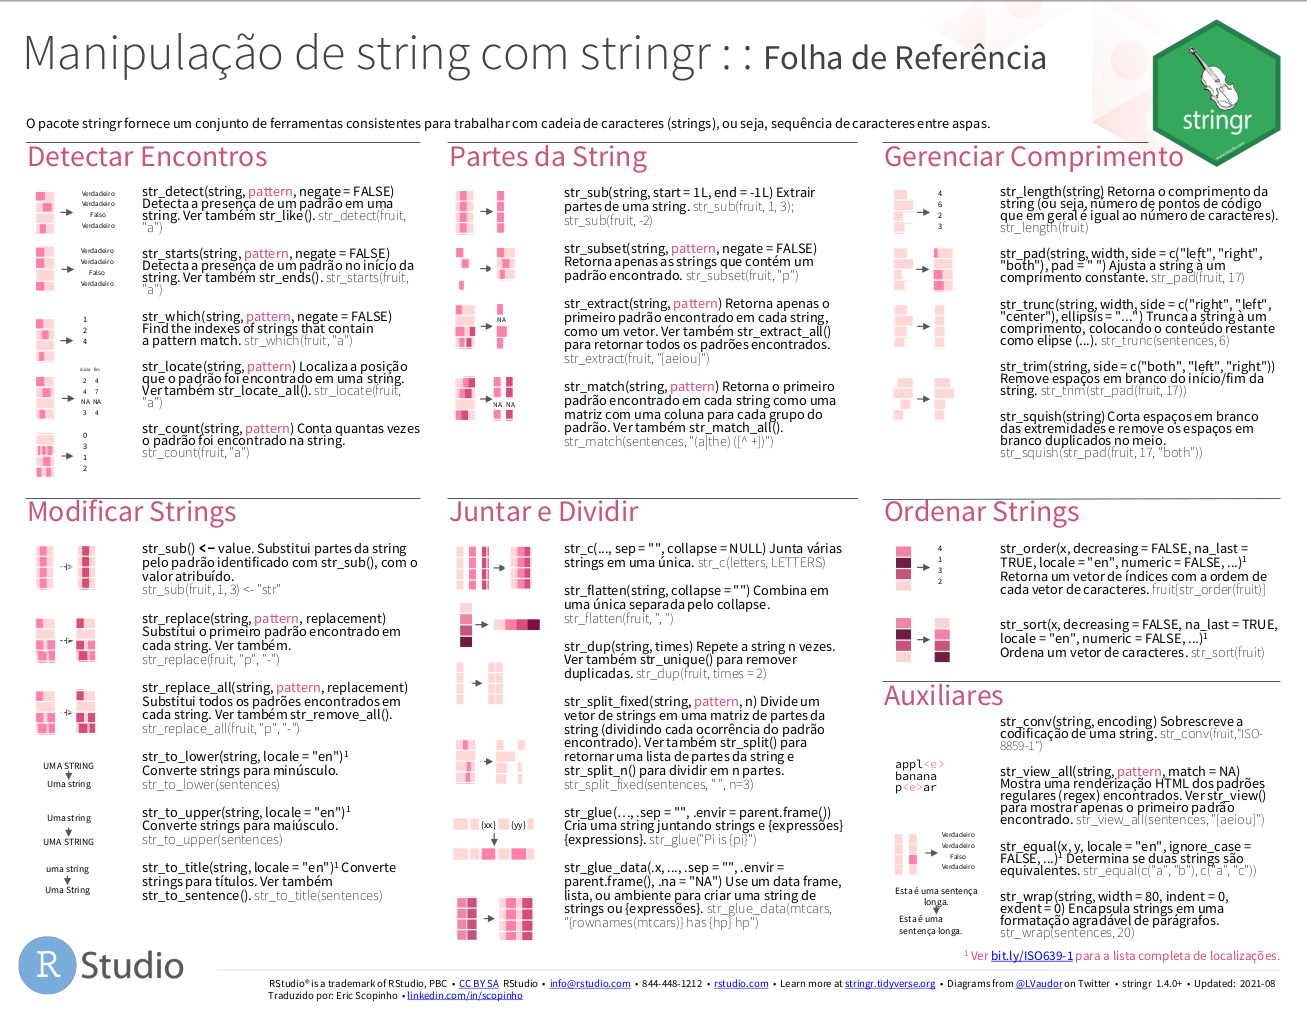
\includegraphics{Manipulacao_Strings/images/cs-stringr-01.png}}

}

\end{figure}

\begin{figure}

{\centering 

\href{images/cs-stringr-02.png}{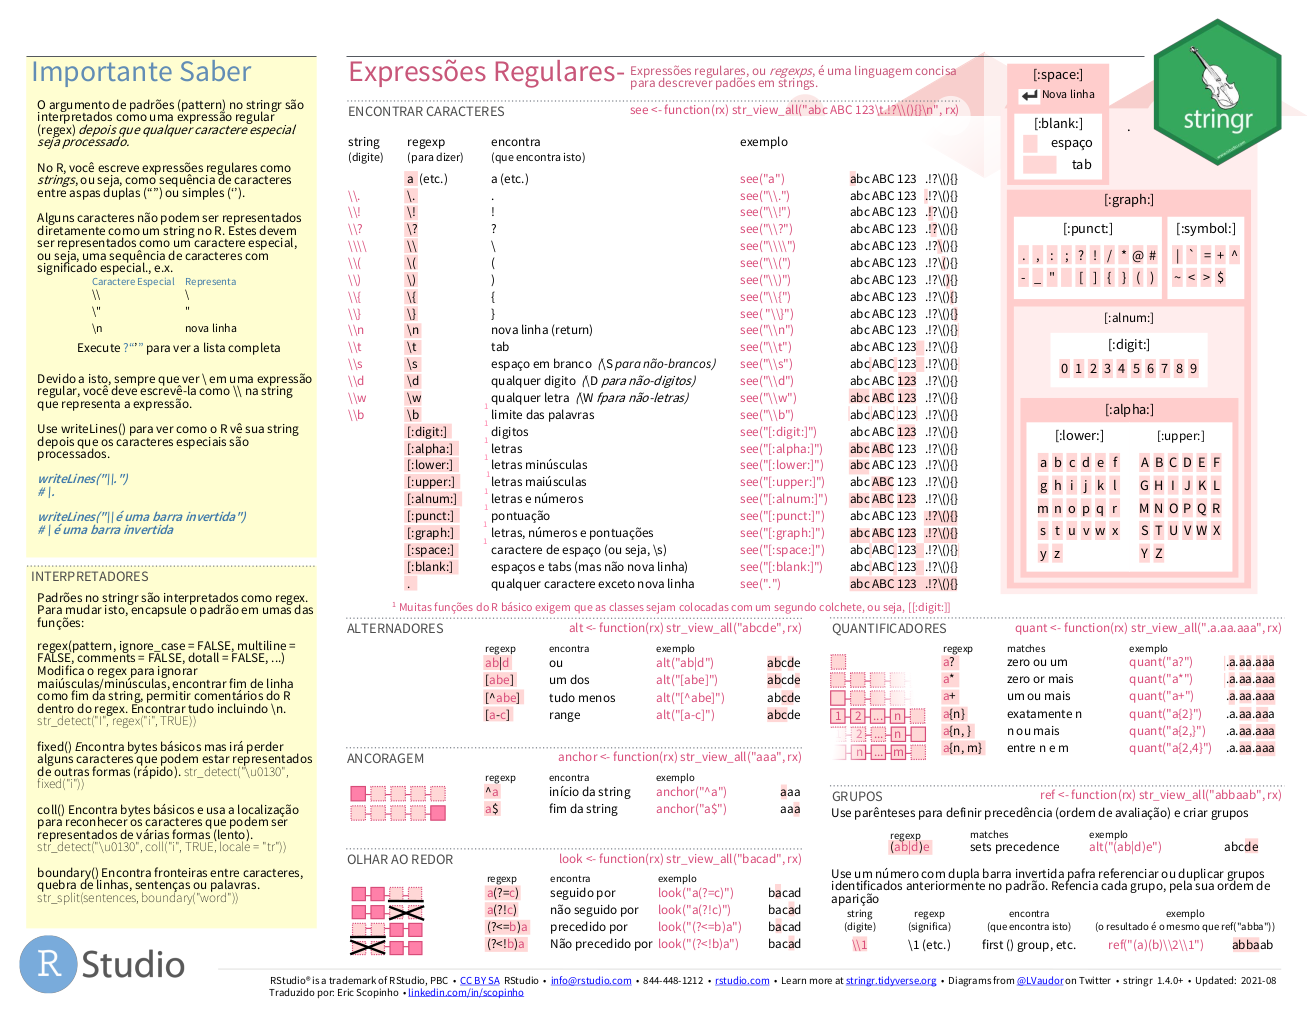
\includegraphics{Manipulacao_Strings/images/cs-stringr-02.png}}

}

\end{figure}

\begin{center}\rule{0.5\linewidth}{0.5pt}\end{center}

Para a maioria dos exemplos utilizaremos as bases de dados
\textbf{fruit} (frutas) que será criado a seguir.

\textbf{FRUIT:} Tabela com nome de frutas (em inglês).

\begin{Shaded}
\begin{Highlighting}[]
\NormalTok{fruit }\OtherTok{\textless{}{-}} \FunctionTok{tibble}\NormalTok{(}\AttributeTok{name =} \FunctionTok{c}\NormalTok{(}\StringTok{"Apple"}\NormalTok{, }\StringTok{"Apricot"}\NormalTok{, }\StringTok{"Avocado"}\NormalTok{, }\StringTok{"Banana"}\NormalTok{, }\StringTok{"Blackberry"}\NormalTok{, }\StringTok{"Blueberry"}\NormalTok{, }\StringTok{"Cherry"}\NormalTok{, }\StringTok{"Coconut"}\NormalTok{, }\StringTok{"Custard{-}Apple"}\NormalTok{, }\StringTok{"Dragonfruit"}\NormalTok{, }\StringTok{"Fig"}\NormalTok{, }\StringTok{"Gooseberry"}\NormalTok{, }\StringTok{"Grapes"}\NormalTok{, }\StringTok{"Guava"}\NormalTok{, }\StringTok{"Jackfruit"}\NormalTok{, }\StringTok{"Java Plum"}\NormalTok{, }\StringTok{"Kiwifruit"}\NormalTok{, }\StringTok{"Lime"}\NormalTok{, }\StringTok{"Mango"}\NormalTok{, }\StringTok{"MuskMelon"}\NormalTok{, }\StringTok{"Olives"}\NormalTok{, }\StringTok{"Orange"}\NormalTok{, }\StringTok{"Papaya"}\NormalTok{, }\StringTok{"Peach"}\NormalTok{, }\StringTok{"Pear"}\NormalTok{, }\StringTok{"Pineapple"}\NormalTok{, }\StringTok{"Pomegranate"}\NormalTok{, }\StringTok{"Strawberry"}\NormalTok{, }\StringTok{"Tamarind"}\NormalTok{, }\StringTok{"Watermelon"}\NormalTok{))}
\NormalTok{fruit }
\end{Highlighting}
\end{Shaded}

\begin{verbatim}
# A tibble: 30 x 1
   name         
   <chr>        
 1 Apple        
 2 Apricot      
 3 Avocado      
 4 Banana       
 5 Blackberry   
 6 Blueberry    
 7 Cherry       
 8 Coconut      
 9 Custard-Apple
10 Dragonfruit  
# ... with 20 more rows
# i Use `print(n = ...)` to see more rows
\end{verbatim}

\begin{center}\rule{0.5\linewidth}{0.5pt}\end{center}

\hypertarget{detectando-combinauxe7uxf5es}{%
\section{Detectando Combinações}\label{detectando-combinauxe7uxf5es}}

O pacote stringr possui uma série de funções para identificar a
ocorrência ou não de \textbf{padrões} de caracteres (patterns).

Na maioria das vezes o mecanismo de interpretação padrão é o de
``Expressão Regular'' (regex). Isto significa que podemos construir um
padrão de caracteres não somente com letras ou números, mas criando
expressões que significam uma combinação mais flexivel no padrão de
busca.

Para maiores informações veja:
\protect\hyperlink{expressuxf5es-regulares}{Expressões Regulares}.

O pacote stringr, possui uma série de funções para manipulação de
strings que veremos a seguir:

\hypertarget{str_detect}{%
\subsubsection{str\_detect}\label{str_detect}}

Use para \textbf{detectar} a presença de um \textbf{padrão} em uma
\textbf{string}.

Por exemplo, para detectar quais frutas tem a letra ``\textbf{a}'',
podemos usar:

\begin{Shaded}
\begin{Highlighting}[]
\FunctionTok{str\_detect}\NormalTok{(fruit}\SpecialCharTok{$}\NormalTok{name, }\StringTok{"a"}\NormalTok{) }
\end{Highlighting}
\end{Shaded}

\begin{verbatim}
 [1] FALSE FALSE  TRUE  TRUE  TRUE FALSE FALSE FALSE  TRUE  TRUE FALSE FALSE
[13]  TRUE  TRUE  TRUE  TRUE FALSE FALSE  TRUE FALSE FALSE  TRUE  TRUE  TRUE
[25]  TRUE  TRUE  TRUE  TRUE  TRUE  TRUE
\end{verbatim}

No exemplo acima, temos \textbf{TRUE} para todas as linhas que contém a
letra ``\textbf{a}'' e \textbf{FALSE} para aquelas que \textbf{não} tem
a letra ``\textbf{a}''.

\begin{tcolorbox}[enhanced jigsaw, rightrule=.15mm, arc=.35mm, coltitle=black, colframe=quarto-callout-important-color-frame, opacityback=0, toprule=.15mm, left=2mm, breakable, colback=white, bottomtitle=1mm, leftrule=.75mm, title=\textcolor{quarto-callout-important-color}{\faExclamation}\hspace{0.5em}{Importante}, colbacktitle=quarto-callout-important-color!10!white, titlerule=0mm, bottomrule=.15mm, toptitle=1mm, opacitybacktitle=0.6]
Observe que o R é sensível à letras maiúsculas e minúsculas. Como
definimos a letra ``a'' (minúscula) como nosso \textbf{padrão} de busca,
ele não retorna TRUE para palavras como ``Apple'' que possui a letra
``A'' maiúscula.
\end{tcolorbox}

Se quisermos criar uma coluna ao lado para facilitar a visualização,
podemos usar a função \textbf{mutate}() do pacote dplyr:

\begin{Shaded}
\begin{Highlighting}[]
\NormalTok{fruit }\SpecialCharTok{|\textgreater{}} 
  \FunctionTok{mutate}\NormalTok{ (}\AttributeTok{Padrao\_Encontrado =} \FunctionTok{str\_detect}\NormalTok{(fruit}\SpecialCharTok{$}\NormalTok{name, }\StringTok{"a"}\NormalTok{)) }
\end{Highlighting}
\end{Shaded}

\begin{verbatim}
# A tibble: 30 x 2
   name          Padrao_Encontrado
   <chr>         <lgl>            
 1 Apple         FALSE            
 2 Apricot       FALSE            
 3 Avocado       TRUE             
 4 Banana        TRUE             
 5 Blackberry    TRUE             
 6 Blueberry     FALSE            
 7 Cherry        FALSE            
 8 Coconut       FALSE            
 9 Custard-Apple TRUE             
10 Dragonfruit   TRUE             
# ... with 20 more rows
# i Use `print(n = ...)` to see more rows
\end{verbatim}

\hypertarget{str_starts}{%
\subsubsection{str\_starts}\label{str_starts}}

Use para determinar \textbf{se há o padrão definido} \textbf{no início}
da string.

Por exemplo, se quisermos identificar quais frutas que começam com o
padrão ``\textbf{Bl}'', usamos:

\begin{Shaded}
\begin{Highlighting}[]
\NormalTok{fruit }\SpecialCharTok{|\textgreater{}} 
  \FunctionTok{mutate}\NormalTok{ (}\AttributeTok{Padrao\_Encontrado\_Inicio =} \FunctionTok{str\_starts}\NormalTok{(fruit}\SpecialCharTok{$}\NormalTok{name, }\StringTok{"Bl"}\NormalTok{)) }
\end{Highlighting}
\end{Shaded}

\begin{verbatim}
# A tibble: 30 x 2
   name          Padrao_Encontrado_Inicio
   <chr>         <lgl>                   
 1 Apple         FALSE                   
 2 Apricot       FALSE                   
 3 Avocado       FALSE                   
 4 Banana        FALSE                   
 5 Blackberry    TRUE                    
 6 Blueberry     TRUE                    
 7 Cherry        FALSE                   
 8 Coconut       FALSE                   
 9 Custard-Apple FALSE                   
10 Dragonfruit   FALSE                   
# ... with 20 more rows
# i Use `print(n = ...)` to see more rows
\end{verbatim}

Veja que apenas as frutas ``Blackberry'' e ``Bluberry'' retornaram
verdadeiro (TRUE).

É comum utilizar a função filter() para filtrar apenas as linhas que
retornam verdadeiro (TRUE) nas funções de detecção de padrão com o
str\_detect, str\_starts, etc. Veja o exemplo abaixo:

\begin{Shaded}
\begin{Highlighting}[]
\NormalTok{fruit }\SpecialCharTok{|\textgreater{}} 
  \FunctionTok{filter}\NormalTok{ (}\FunctionTok{str\_starts}\NormalTok{(name, }\StringTok{"Bl"}\NormalTok{)) }
\end{Highlighting}
\end{Shaded}

\begin{verbatim}
# A tibble: 2 x 1
  name      
  <chr>     
1 Blackberry
2 Blueberry 
\end{verbatim}

\hypertarget{str_which}{%
\subsubsection{str\_which}\label{str_which}}

Use para retornar em \textbf{qual linha} o pdrão foi encontrado.

Por exemplo, supondo que o padrão sejam as letras ``Bl'' (B maiúscula e
l minúscula), usamos:

\begin{Shaded}
\begin{Highlighting}[]
\FunctionTok{str\_which}\NormalTok{(fruit}\SpecialCharTok{$}\NormalTok{name, }\StringTok{"Bl"}\NormalTok{)}
\end{Highlighting}
\end{Shaded}

\begin{verbatim}
[1] 5 6
\end{verbatim}

Neste exemplo, identificamos que os únicos registros que atendem ao
padrão ``Bl'' estão nas linhas 5 e 6 da tabela.

\hypertarget{str_locate}{%
\subsubsection{str\_locate}\label{str_locate}}

Use para \textbf{localizar a posição} do padrão na string.

Por exemplo, se criarmos uma coluna contendo onde, em cada nome de
fruta, o padrão de busca ``er'' é encontrado, usamos:\\

\begin{Shaded}
\begin{Highlighting}[]
\NormalTok{fruit }\SpecialCharTok{|\textgreater{}} 
  \FunctionTok{mutate}\NormalTok{ (Localização}\AttributeTok{\_na\_string =} \FunctionTok{str\_locate}\NormalTok{(name, }\StringTok{"er"}\NormalTok{)) }
\end{Highlighting}
\end{Shaded}

\begin{verbatim}
# A tibble: 30 x 2
   name          Localização_na_string[,"start"] [,"end"]
   <chr>                                   <int>    <int>
 1 Apple                                      NA       NA
 2 Apricot                                    NA       NA
 3 Avocado                                    NA       NA
 4 Banana                                     NA       NA
 5 Blackberry                                  7        8
 6 Blueberry                                   6        7
 7 Cherry                                      3        4
 8 Coconut                                    NA       NA
 9 Custard-Apple                              NA       NA
10 Dragonfruit                                NA       NA
# ... with 20 more rows
# i Use `print(n = ...)` to see more rows
\end{verbatim}

A função str\_locale retorna \textbf{NA} caso o padrão não seja
encontrado na string.

\begin{tcolorbox}[enhanced jigsaw, rightrule=.15mm, arc=.35mm, coltitle=black, colframe=quarto-callout-tip-color-frame, opacityback=0, toprule=.15mm, left=2mm, breakable, colback=white, bottomtitle=1mm, leftrule=.75mm, title=\textcolor{quarto-callout-tip-color}{\faLightbulb}\hspace{0.5em}{Dica}, colbacktitle=quarto-callout-tip-color!10!white, titlerule=0mm, bottomrule=.15mm, toptitle=1mm, opacitybacktitle=0.6]
Ao encontrar o padrão, a str\_locale para imediatamente a busca na
string. Caso precise encontrar todas as posições que o padrão existir na
mesma string, utiliza a \textbf{str\_locale\_all(}).
\end{tcolorbox}

\hypertarget{str_count}{%
\subsubsection{str\_count}\label{str_count}}

Use para identificar o número de vez que o padrão foi encontrado na
string.

Por exemplo, se buscarmos pelo padrão ``na'', identificamos que a fruta
\emph{banana}, possui o padrão três vezes, enquanto a fruta
\emph{pomegranade} apenas uma vez.

\begin{Shaded}
\begin{Highlighting}[]
\NormalTok{fruit }\SpecialCharTok{|\textgreater{}} 
  \FunctionTok{mutate}\NormalTok{ (}\AttributeTok{Vezes\_padrao\_encontrado =} \FunctionTok{str\_count}\NormalTok{(name, }\StringTok{"na"}\NormalTok{)) }
\end{Highlighting}
\end{Shaded}

\begin{verbatim}
# A tibble: 30 x 2
   name          Vezes_padrao_encontrado
   <chr>                           <int>
 1 Apple                               0
 2 Apricot                             0
 3 Avocado                             0
 4 Banana                              2
 5 Blackberry                          0
 6 Blueberry                           0
 7 Cherry                              0
 8 Coconut                             0
 9 Custard-Apple                       0
10 Dragonfruit                         0
# ... with 20 more rows
# i Use `print(n = ...)` to see more rows
\end{verbatim}

\hypertarget{partes-da-string}{%
\section{Partes da String}\label{partes-da-string}}

O pacote stringr possui uma série de funções que permitem obter partes
de uma string baseado em um padrão de busca. Assim como nas funções de
detecção, o interpretador padrão é o regex. Para maiores informações
veja: \protect\hyperlink{expressuxf5es-regulares}{Expressões Regulares}.

\hypertarget{str_sub}{%
\subsubsection{str\_sub}\label{str_sub}}

Use para \textbf{extrair} ou \textbf{substituir} partes de uma string a
partir de um vetor de caracteres.

Por exemplo, para \textbf{extrair} do segundo até o quarto caractere dos
nomes das frutas, usamos:

\begin{Shaded}
\begin{Highlighting}[]
\NormalTok{fruit }\SpecialCharTok{|\textgreater{}} 
  \FunctionTok{mutate}\NormalTok{ (}\AttributeTok{Segundo\_ao\_Quarto\_Caractere =} \FunctionTok{str\_sub}\NormalTok{(name, }\DecValTok{2}\NormalTok{, }\DecValTok{4}\NormalTok{)) }
\end{Highlighting}
\end{Shaded}

\begin{verbatim}
# A tibble: 30 x 2
   name          Segundo_ao_Quarto_Caractere
   <chr>         <chr>                      
 1 Apple         ppl                        
 2 Apricot       pri                        
 3 Avocado       voc                        
 4 Banana        ana                        
 5 Blackberry    lac                        
 6 Blueberry     lue                        
 7 Cherry        her                        
 8 Coconut       oco                        
 9 Custard-Apple ust                        
10 Dragonfruit   rag                        
# ... with 20 more rows
# i Use `print(n = ...)` to see more rows
\end{verbatim}

Se precisarmos variar o início ou fim da extração de parte da string,
podemos passar valores negativos para os parametros start = e/ou end =,
fazendo com que a contagem acontece de trás para frente.

\hypertarget{str_subset}{%
\subsubsection{str\_subset}\label{str_subset}}

Use para retornar as strings que contém o padrão. É equivalente a fazer
str\_detect(x, pattern), porém ao invés de retornar verdadeiro ou falso,
retorna a string.

\begin{Shaded}
\begin{Highlighting}[]
\FunctionTok{str\_subset}\NormalTok{(fruit}\SpecialCharTok{$}\NormalTok{name, }\StringTok{"Bl"}\NormalTok{)}
\end{Highlighting}
\end{Shaded}

\begin{verbatim}
[1] "Blackberry" "Blueberry" 
\end{verbatim}

\hypertarget{str_extract}{%
\subsubsection{str\_extract}\label{str_extract}}

Use para obter o padrão encontrado na string.

Por exemplo, queremos obter parte da string que atenda ao padrão
``erry''. Neste caso, a função irá retornar NA para as strings que não
contém o padrão e o padrão para aquelas que o contém.

\begin{Shaded}
\begin{Highlighting}[]
\NormalTok{fruit }\SpecialCharTok{|\textgreater{}} 
  \FunctionTok{mutate}\NormalTok{ (}\AttributeTok{Str\_Extract =} \FunctionTok{str\_extract}\NormalTok{(name, }\StringTok{"erry"}\NormalTok{)) }
\end{Highlighting}
\end{Shaded}

\begin{verbatim}
# A tibble: 30 x 2
   name          Str_Extract
   <chr>         <chr>      
 1 Apple         <NA>       
 2 Apricot       <NA>       
 3 Avocado       <NA>       
 4 Banana        <NA>       
 5 Blackberry    erry       
 6 Blueberry     erry       
 7 Cherry        erry       
 8 Coconut       <NA>       
 9 Custard-Apple <NA>       
10 Dragonfruit   <NA>       
# ... with 20 more rows
# i Use `print(n = ...)` to see more rows
\end{verbatim}

\hypertarget{str_match}{%
\subsubsection{str\_match}\label{str_match}}

Use para obter os grupos identificados pelo padrão de busca. Ela retorna
uma matriz, onde a primeira coluna retorna a combinação (match) toda e
as demais colunas será uma para cada grupo identificado.

Por exemplo, se buscarmos por dois grupos, sendo o primeiro (Ba) e o
segundo grupo (na), teremos o seguinte resultado:

\begin{Shaded}
\begin{Highlighting}[]
\FunctionTok{str\_match}\NormalTok{(fruit}\SpecialCharTok{$}\NormalTok{name, }\StringTok{"(Ba)(na)"}\NormalTok{) }\SpecialCharTok{|\textgreater{}} 
  \FunctionTok{as\_tibble}\NormalTok{(}\AttributeTok{.name\_repair =} \StringTok{"unique"}\NormalTok{)}
\end{Highlighting}
\end{Shaded}

\begin{verbatim}
# A tibble: 30 x 3
   ...1  ...2  ...3 
   <chr> <chr> <chr>
 1 <NA>  <NA>  <NA> 
 2 <NA>  <NA>  <NA> 
 3 <NA>  <NA>  <NA> 
 4 Bana  Ba    na   
 5 <NA>  <NA>  <NA> 
 6 <NA>  <NA>  <NA> 
 7 <NA>  <NA>  <NA> 
 8 <NA>  <NA>  <NA> 
 9 <NA>  <NA>  <NA> 
10 <NA>  <NA>  <NA> 
# ... with 20 more rows
# i Use `print(n = ...)` to see more rows
\end{verbatim}

\begin{tcolorbox}[enhanced jigsaw, rightrule=.15mm, arc=.35mm, coltitle=black, colframe=quarto-callout-note-color-frame, opacityback=0, toprule=.15mm, left=2mm, breakable, colback=white, bottomtitle=1mm, leftrule=.75mm, title=\textcolor{quarto-callout-note-color}{\faInfo}\hspace{0.5em}{Nota}, colbacktitle=quarto-callout-note-color!10!white, titlerule=0mm, bottomrule=.15mm, toptitle=1mm, opacitybacktitle=0.6]
Os detalhes sobre grupos nos padrões de busca faz parte das expressões
regulares (regex) e estão mais detalhadas na seção:
\protect\hyperlink{expressuxf5es-regulares}{Expressões Regulares}
\end{tcolorbox}

\hypertarget{gerenciando-tamanho}{%
\section{Gerenciando Tamanho}\label{gerenciando-tamanho}}

\hypertarget{str_length}{%
\subsubsection{str\_length}\label{str_length}}

Use para obter o tamanho da string.

Por exemplo, para obtermos o tamanho das strings correspondentes aos
nomes das frutas e adicioná-las em uma coluna chamada ``Tamanho'',
podemos fazer:

\begin{Shaded}
\begin{Highlighting}[]
\NormalTok{fruit }\SpecialCharTok{|\textgreater{}} 
  \FunctionTok{mutate}\NormalTok{(}\AttributeTok{Tamanho =} \FunctionTok{str\_length}\NormalTok{(name)) }
\end{Highlighting}
\end{Shaded}

\begin{verbatim}
# A tibble: 30 x 2
   name          Tamanho
   <chr>           <int>
 1 Apple               5
 2 Apricot             7
 3 Avocado             7
 4 Banana              6
 5 Blackberry         10
 6 Blueberry           9
 7 Cherry              6
 8 Coconut             7
 9 Custard-Apple      13
10 Dragonfruit        11
# ... with 20 more rows
# i Use `print(n = ...)` to see more rows
\end{verbatim}

\hypertarget{str_pad}{%
\subsubsection{str\_pad}\label{str_pad}}

Use para adicionar espaços em branco ao lado (esquerdo, direito, ambos)
da string.

Por exemplo, para adicionar espaços em branco para ajustar em 20
caracteres os nomes das frutas, usamos:

\begin{Shaded}
\begin{Highlighting}[]
\NormalTok{fruit }\SpecialCharTok{|\textgreater{}} \FunctionTok{mutate}\NormalTok{(}\AttributeTok{Tamanho =} \FunctionTok{str\_pad}\NormalTok{(name, }\DecValTok{20}\NormalTok{, }\StringTok{"left"}\NormalTok{)) }\SpecialCharTok{|\textgreater{}} \FunctionTok{as.matrix}\NormalTok{()}
\end{Highlighting}
\end{Shaded}

\begin{verbatim}
      name            Tamanho               
 [1,] "Apple"         "               Apple"
 [2,] "Apricot"       "             Apricot"
 [3,] "Avocado"       "             Avocado"
 [4,] "Banana"        "              Banana"
 [5,] "Blackberry"    "          Blackberry"
 [6,] "Blueberry"     "           Blueberry"
 [7,] "Cherry"        "              Cherry"
 [8,] "Coconut"       "             Coconut"
 [9,] "Custard-Apple" "       Custard-Apple"
[10,] "Dragonfruit"   "         Dragonfruit"
[11,] "Fig"           "                 Fig"
[12,] "Gooseberry"    "          Gooseberry"
[13,] "Grapes"        "              Grapes"
[14,] "Guava"         "               Guava"
[15,] "Jackfruit"     "           Jackfruit"
[16,] "Java Plum"     "           Java Plum"
[17,] "Kiwifruit"     "           Kiwifruit"
[18,] "Lime"          "                Lime"
[19,] "Mango"         "               Mango"
[20,] "MuskMelon"     "           MuskMelon"
[21,] "Olives"        "              Olives"
[22,] "Orange"        "              Orange"
[23,] "Papaya"        "              Papaya"
[24,] "Peach"         "               Peach"
[25,] "Pear"          "                Pear"
[26,] "Pineapple"     "           Pineapple"
[27,] "Pomegranate"   "         Pomegranate"
[28,] "Strawberry"    "          Strawberry"
[29,] "Tamarind"      "            Tamarind"
[30,] "Watermelon"    "          Watermelon"
\end{verbatim}

\hypertarget{str_trunc}{%
\subsubsection{str\_trunc}\label{str_trunc}}

Use para truncar a string em um número fixo de caracteres.

Por exemplo, para truncar os nomes das frutas em até 8 caracteres,
usamos:

\begin{Shaded}
\begin{Highlighting}[]
\NormalTok{fruit }\SpecialCharTok{|\textgreater{}} \FunctionTok{mutate}\NormalTok{(}\AttributeTok{Tamanho =} \FunctionTok{str\_trunc}\NormalTok{(name, }\DecValTok{8}\NormalTok{, }\StringTok{"right"}\NormalTok{)) }\SpecialCharTok{|\textgreater{}} \FunctionTok{as.matrix}\NormalTok{()}
\end{Highlighting}
\end{Shaded}

\begin{verbatim}
      name            Tamanho   
 [1,] "Apple"         "Apple"   
 [2,] "Apricot"       "Apricot" 
 [3,] "Avocado"       "Avocado" 
 [4,] "Banana"        "Banana"  
 [5,] "Blackberry"    "Black..."
 [6,] "Blueberry"     "Blueb..."
 [7,] "Cherry"        "Cherry"  
 [8,] "Coconut"       "Coconut" 
 [9,] "Custard-Apple" "Custa..."
[10,] "Dragonfruit"   "Drago..."
[11,] "Fig"           "Fig"     
[12,] "Gooseberry"    "Goose..."
[13,] "Grapes"        "Grapes"  
[14,] "Guava"         "Guava"   
[15,] "Jackfruit"     "Jackf..."
[16,] "Java Plum"     "Java ..."
[17,] "Kiwifruit"     "Kiwif..."
[18,] "Lime"          "Lime"    
[19,] "Mango"         "Mango"   
[20,] "MuskMelon"     "MuskM..."
[21,] "Olives"        "Olives"  
[22,] "Orange"        "Orange"  
[23,] "Papaya"        "Papaya"  
[24,] "Peach"         "Peach"   
[25,] "Pear"          "Pear"    
[26,] "Pineapple"     "Pinea..."
[27,] "Pomegranate"   "Pomeg..."
[28,] "Strawberry"    "Straw..."
[29,] "Tamarind"      "Tamarind"
[30,] "Watermelon"    "Water..."
\end{verbatim}

\begin{tcolorbox}[enhanced jigsaw, rightrule=.15mm, arc=.35mm, coltitle=black, colframe=quarto-callout-tip-color-frame, opacityback=0, toprule=.15mm, left=2mm, breakable, colback=white, bottomtitle=1mm, leftrule=.75mm, title=\textcolor{quarto-callout-tip-color}{\faLightbulb}\hspace{0.5em}{Dica}, colbacktitle=quarto-callout-tip-color!10!white, titlerule=0mm, bottomrule=.15mm, toptitle=1mm, opacitybacktitle=0.6]
Observe que a função adiciona ``\ldots{}'' para identificar as strings
que tinham mais que o limite definido''. Utilize o parametro ellipsis =
``\ldots{}'' para alterar para outros caracteres.
\end{tcolorbox}

\hypertarget{str_trim}{%
\subsubsection{str\_trim}\label{str_trim}}

Use para remover os espaços em brancos do início em final da string.

\begin{Shaded}
\begin{Highlighting}[]
\NormalTok{string }\OtherTok{\textless{}{-}} \StringTok{"  Aqui temos espaços em branco no início e no final   "}
\FunctionTok{str\_trim}\NormalTok{(string)}
\end{Highlighting}
\end{Shaded}

\begin{verbatim}
[1] "Aqui temos espaços em branco no início e no final"
\end{verbatim}

\hypertarget{str_squish}{%
\subsubsection{str\_squish}\label{str_squish}}

Use para remover espaços em branco no início e final da string e também
espaços em brancos repetidos no meio da string.

\begin{Shaded}
\begin{Highlighting}[]
\NormalTok{string }\OtherTok{\textless{}{-}} \StringTok{"  Aqui temos espaços em       branco no início, no final e repetidos no meio   "}
\FunctionTok{str\_squish}\NormalTok{(string)}
\end{Highlighting}
\end{Shaded}

\begin{verbatim}
[1] "Aqui temos espaços em branco no início, no final e repetidos no meio"
\end{verbatim}

\hypertarget{modificando-string}{%
\section{Modificando String}\label{modificando-string}}

\hypertarget{str_sub-1}{%
\subsubsection{str\_sub}\label{str_sub-1}}

Use para \textbf{extrair} ou \textbf{substituir} partes de uma string a
partir de um vetor de caracteres.

Por exemplo, para \textbf{substituir} do segundo até o quarto caractere
dos nomes das frutas, usamos:

\begin{Shaded}
\begin{Highlighting}[]
\NormalTok{minha\_string }\OtherTok{\textless{}{-}} \StringTok{"Esta é minha string"}\NormalTok{; minha\_string}
\end{Highlighting}
\end{Shaded}

\begin{verbatim}
[1] "Esta é minha string"
\end{verbatim}

\begin{Shaded}
\begin{Highlighting}[]
\FunctionTok{str\_sub}\NormalTok{(minha\_string, }\DecValTok{2}\NormalTok{, }\DecValTok{4}\NormalTok{) }\OtherTok{\textless{}{-}} \StringTok{"XXX"}\NormalTok{; minha\_string}
\end{Highlighting}
\end{Shaded}

\begin{verbatim}
[1] "EXXX é minha string"
\end{verbatim}

\begin{tcolorbox}[enhanced jigsaw, rightrule=.15mm, arc=.35mm, coltitle=black, colframe=quarto-callout-tip-color-frame, opacityback=0, toprule=.15mm, left=2mm, breakable, colback=white, bottomtitle=1mm, leftrule=.75mm, title=\textcolor{quarto-callout-tip-color}{\faLightbulb}\hspace{0.5em}{Dica}, colbacktitle=quarto-callout-tip-color!10!white, titlerule=0mm, bottomrule=.15mm, toptitle=1mm, opacitybacktitle=0.6]
Observe que a função \textbf{str\_sub não é vetorizada}, ou seja, não
recebe ou retorna um vetor como parêmetro.

Desta forma, se quisermos aplicá-la em conjunto com a função
\textbf{mutate}(). Uma alternativa para este tipo de situação, é
utilziar a função \textbf{map}() do \textbf{pacote} \textbf{purrr}.
\end{tcolorbox}

Por exemplo, vamos criar uma função chamada ``substitui\_string''. Esta
função irá utilizar a função str\_sub() de acordo com os parametros
recebidos de str\_troca, inicio e fim. Utilizando a função purrr::map()
iremos iterar através dos nomes das frutas e utilizar a função
substitui\_string() para trocar por ``XX'' os caracteres -2 a -3 de
todos os nomes em uma coluna ao lado.

\begin{Shaded}
\begin{Highlighting}[]
\NormalTok{substitui\_string }\OtherTok{\textless{}{-}} \ControlFlowTok{function}\NormalTok{(str\_origin, str\_troca, inicio, fim)\{}
  \FunctionTok{str\_sub}\NormalTok{(str\_origin, inicio, fim) }\OtherTok{\textless{}{-}}\NormalTok{ str\_troca}
  \FunctionTok{return}\NormalTok{ (str\_origin)}
\NormalTok{\}}

\NormalTok{fruit }\SpecialCharTok{|\textgreater{}} 
  \FunctionTok{mutate}\NormalTok{ (}\AttributeTok{Segundo\_ao\_Quarto\_Caracteres =}\NormalTok{ purrr}\SpecialCharTok{::}\FunctionTok{map\_chr}\NormalTok{ (name, substitui\_string, }\AttributeTok{str\_troca =} \StringTok{"XX"}\NormalTok{, }\AttributeTok{inicio =} \SpecialCharTok{{-}}\DecValTok{3}\NormalTok{, }\AttributeTok{fim =} \SpecialCharTok{{-}}\DecValTok{2}\NormalTok{))}
\end{Highlighting}
\end{Shaded}

\begin{verbatim}
# A tibble: 30 x 2
   name          Segundo_ao_Quarto_Caracteres
   <chr>         <chr>                       
 1 Apple         ApXXe                       
 2 Apricot       ApriXXt                     
 3 Avocado       AvocXXo                     
 4 Banana        BanXXa                      
 5 Blackberry    BlackbeXXy                  
 6 Blueberry     BluebeXXy                   
 7 Cherry        CheXXy                      
 8 Coconut       CocoXXt                     
 9 Custard-Apple Custard-ApXXe               
10 Dragonfruit   DragonfrXXt                 
# ... with 20 more rows
# i Use `print(n = ...)` to see more rows
\end{verbatim}

\begin{tcolorbox}[enhanced jigsaw, rightrule=.15mm, arc=.35mm, coltitle=black, colframe=quarto-callout-note-color-frame, opacityback=0, toprule=.15mm, left=2mm, breakable, colback=white, bottomtitle=1mm, leftrule=.75mm, title=\textcolor{quarto-callout-note-color}{\faInfo}\hspace{0.5em}{Nota}, colbacktitle=quarto-callout-note-color!10!white, titlerule=0mm, bottomrule=.15mm, toptitle=1mm, opacitybacktitle=0.6]
Observe que valores negativos para os parametros start = e/ou end =,
fazem com que a contagem aconteça de trás para frente.
\end{tcolorbox}

\hypertarget{str_replace}{%
\subsubsection{str\_replace}\label{str_replace}}

Use para substituir partes de uma string por outra string de acordo com
o padrão de busca (ex: regex) definido.

\begin{tcolorbox}[enhanced jigsaw, rightrule=.15mm, arc=.35mm, coltitle=black, colframe=quarto-callout-tip-color-frame, opacityback=0, toprule=.15mm, left=2mm, breakable, colback=white, bottomtitle=1mm, leftrule=.75mm, title=\textcolor{quarto-callout-tip-color}{\faLightbulb}\hspace{0.5em}{Dica}, colbacktitle=quarto-callout-tip-color!10!white, titlerule=0mm, bottomrule=.15mm, toptitle=1mm, opacitybacktitle=0.6]
Para saber mais sobre o método de expressão regular (regex) veja:
\protect\hyperlink{expressuxf5es-regulares}{Expressões Regulares} e para
os outros métodos de interpretação, veja
\protect\hyperlink{outras-interpretauxe7uxf5es}{Outras Interpretações}.
\end{tcolorbox}

Por exemplo, vamos definir inicialmente que nosso padrão de busca são as
letras ``er''. Agora vamos substituir este padrão pela string '' XX ''
colocando em uma coluna ao lado usando a função mutate().

\begin{Shaded}
\begin{Highlighting}[]
\NormalTok{fruit }\SpecialCharTok{|\textgreater{}} 
  \FunctionTok{mutate}\NormalTok{ (}\AttributeTok{nomes\_substituidos =} \FunctionTok{str\_replace}\NormalTok{(name, }\StringTok{"er"}\NormalTok{, }\StringTok{" XX "}\NormalTok{)) }
\end{Highlighting}
\end{Shaded}

\begin{verbatim}
# A tibble: 30 x 2
   name          nomes_substituidos
   <chr>         <chr>             
 1 Apple         Apple             
 2 Apricot       Apricot           
 3 Avocado       Avocado           
 4 Banana        Banana            
 5 Blackberry    Blackb XX ry      
 6 Blueberry     Blueb XX ry       
 7 Cherry        Ch XX ry          
 8 Coconut       Coconut           
 9 Custard-Apple Custard-Apple     
10 Dragonfruit   Dragonfruit       
# ... with 20 more rows
# i Use `print(n = ...)` to see more rows
\end{verbatim}

\begin{tcolorbox}[enhanced jigsaw, rightrule=.15mm, arc=.35mm, coltitle=black, colframe=quarto-callout-note-color-frame, opacityback=0, toprule=.15mm, left=2mm, breakable, colback=white, bottomtitle=1mm, leftrule=.75mm, title=\textcolor{quarto-callout-note-color}{\faInfo}\hspace{0.5em}{Nota}, colbacktitle=quarto-callout-note-color!10!white, titlerule=0mm, bottomrule=.15mm, toptitle=1mm, opacitybacktitle=0.6]
Note que diferente da função str\_sub(), a função str\_replace() é
vetorizada, com isto não precisamos utilizar o purrr:map para retornar
um vetor.
\end{tcolorbox}

\hypertarget{str_replace_all}{%
\subsubsection{str\_replace\_all}\label{str_replace_all}}

Use para substituir partes de uma string por outra string de acordo com
o padrão de busca (ex: regex) definido em TODAS as vezes que o padrão
for encontrado.

Por exemplo, vamos definir inicialmente que nosso padrão de busca são as
letras ``na''. Agora vamos substituir este padrão pela string '' XX ''
colocando em uma coluna ao lado usando a função mutate().

\begin{Shaded}
\begin{Highlighting}[]
\NormalTok{fruit }\SpecialCharTok{|\textgreater{}} 
  \FunctionTok{mutate}\NormalTok{ (}\AttributeTok{nomes\_substituidos =} \FunctionTok{str\_replace\_all}\NormalTok{(name, }\StringTok{"an"}\NormalTok{, }\StringTok{" XX "}\NormalTok{))}
\end{Highlighting}
\end{Shaded}

\begin{verbatim}
# A tibble: 30 x 2
   name          nomes_substituidos
   <chr>         <chr>             
 1 Apple         Apple             
 2 Apricot       Apricot           
 3 Avocado       Avocado           
 4 Banana        B XX  XX a        
 5 Blackberry    Blackberry        
 6 Blueberry     Blueberry         
 7 Cherry        Cherry            
 8 Coconut       Coconut           
 9 Custard-Apple Custard-Apple     
10 Dragonfruit   Dragonfruit       
# ... with 20 more rows
# i Use `print(n = ...)` to see more rows
\end{verbatim}

Note que se tivessemo utilizado a função str\_replace ao invés da
str\_replace\_all, a palavra ``\textbf{Banana}'' retornaria ``B\textbf{a
XX na}'', pois ela substituiria apenas a primeira vez que o padrão fosse
encontrado.

\hypertarget{str_to_lower}{%
\subsubsection{str\_to\_lower}\label{str_to_lower}}

Use para colocar a string em letras minúsculas.

\begin{Shaded}
\begin{Highlighting}[]
\NormalTok{fruit }\SpecialCharTok{|\textgreater{}} 
  \FunctionTok{mutate}\NormalTok{ (}\AttributeTok{tolowe =} \FunctionTok{str\_to\_lower}\NormalTok{(name)) }
\end{Highlighting}
\end{Shaded}

\begin{verbatim}
# A tibble: 30 x 2
   name          tolowe       
   <chr>         <chr>        
 1 Apple         apple        
 2 Apricot       apricot      
 3 Avocado       avocado      
 4 Banana        banana       
 5 Blackberry    blackberry   
 6 Blueberry     blueberry    
 7 Cherry        cherry       
 8 Coconut       coconut      
 9 Custard-Apple custard-apple
10 Dragonfruit   dragonfruit  
# ... with 20 more rows
# i Use `print(n = ...)` to see more rows
\end{verbatim}

\hypertarget{str_to_upper}{%
\subsubsection{str\_to\_upper}\label{str_to_upper}}

Use para colocar a string em letras maiúsculas.

\begin{Shaded}
\begin{Highlighting}[]
\NormalTok{fruit }\SpecialCharTok{|\textgreater{}} 
  \FunctionTok{mutate}\NormalTok{ (}\AttributeTok{toupper =} \FunctionTok{str\_to\_upper}\NormalTok{(name)) }
\end{Highlighting}
\end{Shaded}

\begin{verbatim}
# A tibble: 30 x 2
   name          toupper      
   <chr>         <chr>        
 1 Apple         APPLE        
 2 Apricot       APRICOT      
 3 Avocado       AVOCADO      
 4 Banana        BANANA       
 5 Blackberry    BLACKBERRY   
 6 Blueberry     BLUEBERRY    
 7 Cherry        CHERRY       
 8 Coconut       COCONUT      
 9 Custard-Apple CUSTARD-APPLE
10 Dragonfruit   DRAGONFRUIT  
# ... with 20 more rows
# i Use `print(n = ...)` to see more rows
\end{verbatim}

\hypertarget{str_to_title}{%
\subsubsection{str\_to\_title}\label{str_to_title}}

Use para colocar a string com a primeira letra maiúscula e as demais em
letras minúsculas de cada palavra.

\begin{Shaded}
\begin{Highlighting}[]
\NormalTok{fruit }\SpecialCharTok{|\textgreater{}} 
  \FunctionTok{mutate}\NormalTok{ (}\AttributeTok{totitle=} \FunctionTok{str\_to\_title}\NormalTok{(name)) }
\end{Highlighting}
\end{Shaded}

\begin{verbatim}
# A tibble: 30 x 2
   name          totitle      
   <chr>         <chr>        
 1 Apple         Apple        
 2 Apricot       Apricot      
 3 Avocado       Avocado      
 4 Banana        Banana       
 5 Blackberry    Blackberry   
 6 Blueberry     Blueberry    
 7 Cherry        Cherry       
 8 Coconut       Coconut      
 9 Custard-Apple Custard-Apple
10 Dragonfruit   Dragonfruit  
# ... with 20 more rows
# i Use `print(n = ...)` to see more rows
\end{verbatim}

\hypertarget{juntando-e-dividindo}{%
\section{Juntando e Dividindo}\label{juntando-e-dividindo}}

\hypertarget{str_c}{%
\subsubsection{str\_c}\label{str_c}}

Use para juntar várias strings em uma única string.

Para exemplificar, vamos criar uma segunda coluna em nossa tabela de
frutas.

\begin{Shaded}
\begin{Highlighting}[]
\CommentTok{\# Nova coluna com uma string qualquer }
\NormalTok{col\_nova }\OtherTok{\textless{}{-}} \FunctionTok{bind\_cols}\NormalTok{(}\FunctionTok{c}\NormalTok{(letters, LETTERS), }\FunctionTok{seq}\NormalTok{(}\DecValTok{1}\SpecialCharTok{:}\DecValTok{52}\NormalTok{), }\FunctionTok{seq}\NormalTok{(}\DecValTok{1}\SpecialCharTok{:}\DecValTok{52}\NormalTok{), }\FunctionTok{c}\NormalTok{(letters, LETTERS))}
\NormalTok{col\_nova }\OtherTok{\textless{}{-}}\NormalTok{ col\_nova }\SpecialCharTok{|\textgreater{}} 
  \FunctionTok{unite}\NormalTok{(nova\_string, }\FunctionTok{names}\NormalTok{(col\_nova)) }\SpecialCharTok{|\textgreater{}} 
  \FunctionTok{slice}\NormalTok{ (}\AttributeTok{n =} \DecValTok{1}\SpecialCharTok{:}\DecValTok{30}\NormalTok{) }
\NormalTok{frutas }\OtherTok{\textless{}{-}} \FunctionTok{bind\_cols}\NormalTok{ (fruit, col\_nova)}

\CommentTok{\#Concatenando ambas colunas}
\NormalTok{  frutas }\SpecialCharTok{|\textgreater{}} 
  \FunctionTok{mutate}\NormalTok{ ( }\AttributeTok{str\_c =} \FunctionTok{str\_c}\NormalTok{(name, nova\_string)) }
\end{Highlighting}
\end{Shaded}

\begin{verbatim}
# A tibble: 30 x 3
   name          nova_string str_c               
   <chr>         <chr>       <chr>               
 1 Apple         a_1_1_a     Applea_1_1_a        
 2 Apricot       b_2_2_b     Apricotb_2_2_b      
 3 Avocado       c_3_3_c     Avocadoc_3_3_c      
 4 Banana        d_4_4_d     Bananad_4_4_d       
 5 Blackberry    e_5_5_e     Blackberrye_5_5_e   
 6 Blueberry     f_6_6_f     Blueberryf_6_6_f    
 7 Cherry        g_7_7_g     Cherryg_7_7_g       
 8 Coconut       h_8_8_h     Coconuth_8_8_h      
 9 Custard-Apple i_9_9_i     Custard-Applei_9_9_i
10 Dragonfruit   j_10_10_j   Dragonfruitj_10_10_j
# ... with 20 more rows
# i Use `print(n = ...)` to see more rows
\end{verbatim}

\begin{tcolorbox}[enhanced jigsaw, rightrule=.15mm, arc=.35mm, coltitle=black, colframe=quarto-callout-tip-color-frame, opacityback=0, toprule=.15mm, left=2mm, breakable, colback=white, bottomtitle=1mm, leftrule=.75mm, title=\textcolor{quarto-callout-tip-color}{\faLightbulb}\hspace{0.5em}{Dica}, colbacktitle=quarto-callout-tip-color!10!white, titlerule=0mm, bottomrule=.15mm, toptitle=1mm, opacitybacktitle=0.6]
Use o parametro \textbf{sep =} para definir um caractere de separação
quando juntar as strings se desejar.
\end{tcolorbox}

\hypertarget{str_flatten}{%
\subsubsection{str\_flatten}\label{str_flatten}}

Use para ``achatar'' o vetor de string. O parametro collapse = ``\,''
pode ser alterado para incluir um caractere específico enquanto ocorre o
processo.

Por exemplo, temos uma string ``Bom dia''. Neste caso, temos um vetor de
caracteres de tamanho 7 (``B'' ``o'' ``m'' '' '' ``d'' ``i'' ``a''). A
função flatten irá achatar este vetor e retornar apenas uma string com
um único vetor (``Bom dia'').

\begin{Shaded}
\begin{Highlighting}[]
\NormalTok{minha\_string }\OtherTok{\textless{}{-}} \FunctionTok{c}\NormalTok{(}\StringTok{"B"}\NormalTok{,}\StringTok{"o"}\NormalTok{,}\StringTok{"m"}\NormalTok{,}\StringTok{" "}\NormalTok{,}\StringTok{"d"}\NormalTok{,}\StringTok{"i"}\NormalTok{,}\StringTok{"a"}\NormalTok{)}
\FunctionTok{length}\NormalTok{ (minha\_string); minha\_string}
\end{Highlighting}
\end{Shaded}

\begin{verbatim}
[1] 7
\end{verbatim}

\begin{verbatim}
[1] "B" "o" "m" " " "d" "i" "a"
\end{verbatim}

\begin{Shaded}
\begin{Highlighting}[]
\NormalTok{minha\_string }\OtherTok{\textless{}{-}} \FunctionTok{str\_flatten}\NormalTok{(minha\_string)}
\FunctionTok{length}\NormalTok{ (minha\_string); minha\_string}
\end{Highlighting}
\end{Shaded}

\begin{verbatim}
[1] 1
\end{verbatim}

\begin{verbatim}
[1] "Bom dia"
\end{verbatim}

\hypertarget{str_dup}{%
\subsubsection{str\_dup}\label{str_dup}}

Use para duplicar uma string determinado número de vezes.

\begin{Shaded}
\begin{Highlighting}[]
\NormalTok{fruit }\SpecialCharTok{|\textgreater{}} 
  \FunctionTok{mutate}\NormalTok{ (}\AttributeTok{str\_dup =} \FunctionTok{str\_dup}\NormalTok{(name, }\DecValTok{3}\NormalTok{)) }
\end{Highlighting}
\end{Shaded}

\begin{verbatim}
# A tibble: 30 x 2
   name          str_dup                                
   <chr>         <chr>                                  
 1 Apple         AppleAppleApple                        
 2 Apricot       ApricotApricotApricot                  
 3 Avocado       AvocadoAvocadoAvocado                  
 4 Banana        BananaBananaBanana                     
 5 Blackberry    BlackberryBlackberryBlackberry         
 6 Blueberry     BlueberryBlueberryBlueberry            
 7 Cherry        CherryCherryCherry                     
 8 Coconut       CoconutCoconutCoconut                  
 9 Custard-Apple Custard-AppleCustard-AppleCustard-Apple
10 Dragonfruit   DragonfruitDragonfruitDragonfruit      
# ... with 20 more rows
# i Use `print(n = ...)` to see more rows
\end{verbatim}

\hypertarget{str_split_fixed}{%
\subsubsection{str\_split\_fixed}\label{str_split_fixed}}

Use para ``quebrar'' um string em partes. A funçao \textbf{str\_split}()
retorna uma string dividida enquanto a funçao
\textbf{str\_split\_fixed}() retorna uma matriz de caracteres com número
fixo de colunas.

Por exemplo, vamos usar a mesma tabela usada no exemplo da funçao
\protect\hyperlink{str_c}{str\_c} chamada frutas (na fruit). Iremos
``quebrar as strings da coluna''nova\_string'' usando oseparator ``\_''.
Como temos exatamente o mesmo número de sperador em todas as strings, a
funções irá nos retornar um vetor de caracteres de tamanho 4.

\begin{Shaded}
\begin{Highlighting}[]
\NormalTok{frutas }\SpecialCharTok{|\textgreater{}} 
  \FunctionTok{mutate}\NormalTok{ (}\AttributeTok{str\_split =} \FunctionTok{str\_split}\NormalTok{(nova\_string, }\StringTok{"\_"}\NormalTok{)) }\SpecialCharTok{|\textgreater{}} 
  \FunctionTok{pull}\NormalTok{(str\_split)}
\end{Highlighting}
\end{Shaded}

\begin{verbatim}
[[1]]
[1] "a" "1" "1" "a"

[[2]]
[1] "b" "2" "2" "b"

[[3]]
[1] "c" "3" "3" "c"

[[4]]
[1] "d" "4" "4" "d"

[[5]]
[1] "e" "5" "5" "e"

[[6]]
[1] "f" "6" "6" "f"

[[7]]
[1] "g" "7" "7" "g"

[[8]]
[1] "h" "8" "8" "h"

[[9]]
[1] "i" "9" "9" "i"

[[10]]
[1] "j"  "10" "10" "j" 

[[11]]
[1] "k"  "11" "11" "k" 

[[12]]
[1] "l"  "12" "12" "l" 

[[13]]
[1] "m"  "13" "13" "m" 

[[14]]
[1] "n"  "14" "14" "n" 

[[15]]
[1] "o"  "15" "15" "o" 

[[16]]
[1] "p"  "16" "16" "p" 

[[17]]
[1] "q"  "17" "17" "q" 

[[18]]
[1] "r"  "18" "18" "r" 

[[19]]
[1] "s"  "19" "19" "s" 

[[20]]
[1] "t"  "20" "20" "t" 

[[21]]
[1] "u"  "21" "21" "u" 

[[22]]
[1] "v"  "22" "22" "v" 

[[23]]
[1] "w"  "23" "23" "w" 

[[24]]
[1] "x"  "24" "24" "x" 

[[25]]
[1] "y"  "25" "25" "y" 

[[26]]
[1] "z"  "26" "26" "z" 

[[27]]
[1] "A"  "27" "27" "A" 

[[28]]
[1] "B"  "28" "28" "B" 

[[29]]
[1] "C"  "29" "29" "C" 

[[30]]
[1] "D"  "30" "30" "D" 
\end{verbatim}

Se quisermos ``quebrar'' uma string usando um separador e já gerarmos as
respectivas colunas em uma tabela, podemos usar a função
str\_split\_fixed(), extrairmos as respectivas matrizes e adicionarmos
como colunas na tabela, podemos fazer: .

\hypertarget{str_glue}{%
\subsubsection{str\_glue}\label{str_glue}}

Use para interpolar/formatar uma string.

Por exemplo, se tivermos duas strings: s1 = ``Fulano'' e s2 = ``da
Silva''. Podemos ``colar'' estas strings usando a função
\textbf{str\_glue}().

\begin{Shaded}
\begin{Highlighting}[]
\NormalTok{s1 }\OtherTok{\textless{}{-}} \StringTok{"Fulano"}
\NormalTok{s2 }\OtherTok{\textless{}{-}} \StringTok{"da Silva"}
\FunctionTok{str\_glue}\NormalTok{(}\StringTok{"\{s1\}"}\NormalTok{,}\StringTok{" "}\NormalTok{, }\StringTok{"\{s2\}"}\NormalTok{)}
\end{Highlighting}
\end{Shaded}

\begin{verbatim}
Fulano da Silva
\end{verbatim}

Podemos também juntar strings fixas e variáveis como no exemplo abaixo.

\begin{Shaded}
\begin{Highlighting}[]
\NormalTok{s1 }\OtherTok{\textless{}{-}} \StringTok{"Fulano"}
\NormalTok{s2 }\OtherTok{\textless{}{-}} \StringTok{"da Silva"}
\FunctionTok{str\_glue}\NormalTok{(}\StringTok{"Meu nome é \{s1\}"}\NormalTok{,}\StringTok{" "}\NormalTok{, }\StringTok{"\{s2\}"}\NormalTok{)}
\end{Highlighting}
\end{Shaded}

\begin{verbatim}
Meu nome é Fulano da Silva
\end{verbatim}

\hypertarget{str_glue_data}{%
\subsubsection{str\_glue\_data}\label{str_glue_data}}

É similar a função \href{}{str\_glue}, mas adequada a objetos de dados.

Por exemplo, vamos juntar o nome das frutas, o nome da linha da tabela
que ela está e mais uma string fixa:

\begin{Shaded}
\begin{Highlighting}[]
\NormalTok{fruit }\SpecialCharTok{|\textgreater{}} \FunctionTok{str\_glue\_data}\NormalTok{(}\StringTok{"A \{name\} é uma fruta."}\NormalTok{) }
\end{Highlighting}
\end{Shaded}

\begin{verbatim}
A Apple é uma fruta.
A Apricot é uma fruta.
A Avocado é uma fruta.
A Banana é uma fruta.
A Blackberry é uma fruta.
A Blueberry é uma fruta.
A Cherry é uma fruta.
A Coconut é uma fruta.
A Custard-Apple é uma fruta.
A Dragonfruit é uma fruta.
A Fig é uma fruta.
A Gooseberry é uma fruta.
A Grapes é uma fruta.
A Guava é uma fruta.
A Jackfruit é uma fruta.
A Java Plum é uma fruta.
A Kiwifruit é uma fruta.
A Lime é uma fruta.
A Mango é uma fruta.
A MuskMelon é uma fruta.
A Olives é uma fruta.
A Orange é uma fruta.
A Papaya é uma fruta.
A Peach é uma fruta.
A Pear é uma fruta.
A Pineapple é uma fruta.
A Pomegranate é uma fruta.
A Strawberry é uma fruta.
A Tamarind é uma fruta.
A Watermelon é uma fruta.
\end{verbatim}

\hypertarget{ordenando-string}{%
\section{Ordenando String}\label{ordenando-string}}

\hypertarget{str_order}{%
\subsubsection{str\_order}\label{str_order}}

Use para sequenciar um vetor de caracteres.

Por exemplo, para colocar em sequência de forma decrescente os nomes da
frutas, podemos usar:

\begin{Shaded}
\begin{Highlighting}[]
  \FunctionTok{str\_order}\NormalTok{(fruit}\SpecialCharTok{$}\NormalTok{name, }\AttributeTok{decreasing =} \ConstantTok{TRUE}\NormalTok{)}
\end{Highlighting}
\end{Shaded}

\begin{verbatim}
 [1] 30 29 28 27 26 25 24 23 22 21 20 19 18 17 16 15 14 13 12 11 10  9  8  7  6
[26]  5  4  3  2  1
\end{verbatim}

O resultado será uma sequência (descrescente) em que cada item do vetor
está.

\hypertarget{str_sort}{%
\subsubsection{str\_sort}\label{str_sort}}

Use para ordenar um vetor de caracteres.

Por exemplo, para ordenar de forma decrescente os nomes da frutas,
podemos usar:

\begin{Shaded}
\begin{Highlighting}[]
\FunctionTok{str\_sort}\NormalTok{(fruit}\SpecialCharTok{$}\NormalTok{name, }\AttributeTok{decreasing =} \ConstantTok{TRUE}\NormalTok{) }\SpecialCharTok{|\textgreater{}} 
  \FunctionTok{as\_tibble}\NormalTok{(}\AttributeTok{.name\_repair =} \StringTok{"unique"}\NormalTok{) }
\end{Highlighting}
\end{Shaded}

\begin{verbatim}
# A tibble: 30 x 1
   value      
   <chr>      
 1 Watermelon 
 2 Tamarind   
 3 Strawberry 
 4 Pomegranate
 5 Pineapple  
 6 Pear       
 7 Peach      
 8 Papaya     
 9 Orange     
10 Olives     
# ... with 20 more rows
# i Use `print(n = ...)` to see more rows
\end{verbatim}

\hypertarget{auxiliares}{%
\section{Auxiliares}\label{auxiliares}}

\hypertarget{str_conv}{%
\subsubsection{str\_conv}\label{str_conv}}

Use para converter o ``encode'' de uma string.

\begin{Shaded}
\begin{Highlighting}[]
\NormalTok{x }\OtherTok{\textless{}{-}} \FunctionTok{rawToChar}\NormalTok{(}\FunctionTok{as.raw}\NormalTok{(}\DecValTok{177}\NormalTok{))}
\NormalTok{x}
\end{Highlighting}
\end{Shaded}

\begin{verbatim}
[1] "\xb1"
\end{verbatim}

\begin{Shaded}
\begin{Highlighting}[]
\FunctionTok{str\_conv}\NormalTok{(x, }\StringTok{"ISO{-}8859{-}2"}\NormalTok{) }\CommentTok{\# Polones a com cedilha"}
\end{Highlighting}
\end{Shaded}

\begin{verbatim}
[1] "ą"
\end{verbatim}

\begin{Shaded}
\begin{Highlighting}[]
\FunctionTok{str\_conv}\NormalTok{(x, }\StringTok{"ISO{-}8859{-}1"}\NormalTok{) }\CommentTok{\# Mais{-}Menos}
\end{Highlighting}
\end{Shaded}

\begin{verbatim}
[1] "±"
\end{verbatim}

\hypertarget{str_view_all}{%
\subsubsection{str\_view\_all}\label{str_view_all}}

Use para ver os valores encontrados na string de acordo com um padrão de
busca.

Por exemplo, se tivermos o padrão de busca como ``er'', podemos ver onde
na strings ele é encontrado.

\begin{Shaded}
\begin{Highlighting}[]
\FunctionTok{str\_view}\NormalTok{(}\FunctionTok{c}\NormalTok{(}\StringTok{"Banana"}\NormalTok{, }\StringTok{"Blueberry"}\NormalTok{, }\StringTok{"Blackberry"}\NormalTok{), }\StringTok{"er"}\NormalTok{) }
\end{Highlighting}
\end{Shaded}

\begin{tcolorbox}[enhanced jigsaw, rightrule=.15mm, arc=.35mm, coltitle=black, colframe=quarto-callout-note-color-frame, opacityback=0, toprule=.15mm, left=2mm, breakable, colback=white, bottomtitle=1mm, leftrule=.75mm, title=\textcolor{quarto-callout-note-color}{\faInfo}\hspace{0.5em}{Nota}, colbacktitle=quarto-callout-note-color!10!white, titlerule=0mm, bottomrule=.15mm, toptitle=1mm, opacitybacktitle=0.6]
A função \textbf{str\_view\_all}(), mostrará \textbf{todos} os encontros
na string, se quiser para a busca do padrão no \textbf{primeiro}
encontro, usa \textbf{str\_view}().
\end{tcolorbox}

\hypertarget{str_wrap}{%
\subsubsection{str\_wrap}\label{str_wrap}}

Use para formatar uma string em parágrafos.

\begin{Shaded}
\begin{Highlighting}[]
\NormalTok{thanks\_path }\OtherTok{\textless{}{-}} \FunctionTok{file.path}\NormalTok{(}\FunctionTok{R.home}\NormalTok{(}\StringTok{"doc"}\NormalTok{), }\StringTok{"THANKS"}\NormalTok{)}
\NormalTok{thanks }\OtherTok{\textless{}{-}} \FunctionTok{str\_c}\NormalTok{(}\FunctionTok{readLines}\NormalTok{(thanks\_path), }\AttributeTok{collapse =} \StringTok{"}\SpecialCharTok{\textbackslash{}n}\StringTok{"}\NormalTok{)}
\NormalTok{thanks }\OtherTok{\textless{}{-}} \FunctionTok{word}\NormalTok{(thanks, }\DecValTok{1}\NormalTok{, }\DecValTok{3}\NormalTok{, }\FunctionTok{fixed}\NormalTok{(}\StringTok{"}\SpecialCharTok{\textbackslash{}n\textbackslash{}n}\StringTok{"}\NormalTok{))}
\FunctionTok{cat}\NormalTok{(}\FunctionTok{str\_wrap}\NormalTok{(thanks, }\AttributeTok{width =} \DecValTok{60}\NormalTok{, }\AttributeTok{indent =} \DecValTok{2}\NormalTok{), }\StringTok{"}\SpecialCharTok{\textbackslash{}n}\StringTok{"}\NormalTok{)}
\end{Highlighting}
\end{Shaded}

\begin{verbatim}
  R would not be what it is today without the invaluable
help of these people outside of the (former and current)
R Core team, who contributed by donating code, bug fixes
and documentation: Valerio Aimale, Suharto Anggono, Thomas
Baier, Gabe Becker, Henrik Bengtsson, Roger Bivand, Ben
Bolker, David Brahm, G"oran Brostr"om, Patrick Burns,
Vince Carey, Saikat DebRoy, Matt Dowle, Brian D'Urso,
Lyndon Drake, Dirk Eddelbuettel, Claus Ekstrom, Sebastian
Fischmeister, John Fox, Paul Gilbert, Yu Gong, Gabor
Grothendieck, Frank E Harrell Jr, Peter M. Haverty,
Torsten Hothorn, Robert King, Kjetil Kjernsmo, Roger
Koenker, Philippe Lambert, Jan de Leeuw, Jim Lindsey,
Patrick Lindsey, Catherine Loader, Gordon Maclean, Arni
Magnusson, John Maindonald, David Meyer, Ei-ji Nakama,
Jens Oehlschl"agel, Steve Oncley, Richard O'Keefe, Hubert
Palme, Roger D. Peng, Jose' C. Pinheiro, Tony Plate, Anthony
Rossini, Jonathan Rougier, Petr Savicky, Guenther Sawitzki,
Marc Schwartz, Arun Srinivasan, Detlef Steuer, Bill Simpson,
Gordon Smyth, Adrian Trapletti, Terry Therneau, Rolf Turner,
Bill Venables, Gregory R. Warnes, Andreas Weingessel, Morten
Welinder, James Wettenhall, Simon Wood, and Achim Zeileis.
Others have written code that has been adopted by R and is
acknowledged in the code files, including 
\end{verbatim}

\hypertarget{expressuxf5es-regulares}{%
\section{Expressões Regulares}\label{expressuxf5es-regulares}}

Padrões de buscas são interpretados na funções do pacote stringr como
Expressões Regulares (regex). Ou seja, quando uma função possui o
parametro \textbf{pattern =}, significa que o interpretador irá entendem
como uma expressão regular por padrão. Você pode alterar o
interpretadores para outros tipos se necessário. Para saber mais sobre
isso, acesse \protect\hyperlink{outras-interpretauxe7uxf5es}{Outras
Interpretações}.

\textbf{Expressão Regular} é uma sequência de caracteres que especificam
um padrão de busca em uma string.

Lembre-se que no R, você escreve uma expressão regular como um string,
ou seja, uma sequência de caracteres entre aspas simples ' ou duplas ``.

Alguns caracteres de uma expressão regular não podem ser representados
diretamente como uma string no R.

Estes são conhecidos como caracteres especiais e são uma sequência de
caracteres que tem um significado específico.

Por exemplo:

\begin{longtable}[]{@{}ll@{}}
\toprule()
Caracteres Especiais & Representa \\
\midrule()
\endhead
\textbackslash\textbackslash{} & \textbackslash{} \\
\textbackslash'' & '' \\
\textbackslash? & ? \\
\bottomrule()
\end{longtable}

\begin{tcolorbox}[enhanced jigsaw, rightrule=.15mm, arc=.35mm, coltitle=black, colframe=quarto-callout-tip-color-frame, opacityback=0, toprule=.15mm, left=2mm, breakable, colback=white, bottomtitle=1mm, leftrule=.75mm, title=\textcolor{quarto-callout-tip-color}{\faLightbulb}\hspace{0.5em}{Dica}, colbacktitle=quarto-callout-tip-color!10!white, titlerule=0mm, bottomrule=.15mm, toptitle=1mm, opacitybacktitle=0.6]
Para obter a lista completa, digite ? ``'''.
\end{tcolorbox}

Devido a isto, sempre que aparecer uma barra invertida (
\textbackslash{} ) em uma expressão regular, você deve digitar duas
barras ( \textbackslash\textbackslash{} ) na strings da expressão.

Isto é uma particularidade do R e outras linguagens isto pode não ser
necessário.

Use a função \textbf{writeLines}() para ver como o R vê sua string
depois dos caracteres especiais forem lido.

\begin{Shaded}
\begin{Highlighting}[]
\FunctionTok{writeLines}\NormalTok{(}\StringTok{"}\SpecialCharTok{\textbackslash{}\textbackslash{}}\StringTok{."}\NormalTok{)}
\end{Highlighting}
\end{Shaded}

\begin{verbatim}
\.
\end{verbatim}

\begin{Shaded}
\begin{Highlighting}[]
\FunctionTok{writeLines}\NormalTok{(}\StringTok{"}\SpecialCharTok{\textbackslash{}\textbackslash{}}\StringTok{"}\NormalTok{)}
\end{Highlighting}
\end{Shaded}

\begin{verbatim}
\
\end{verbatim}

Como exemplo inicial, vamos utilizar a função \textbf{str\_extract}()
que recebe um string como parametro e também aceita o padrão de busca
como outro parametro.

Iremos definir nosso \textbf{padrão} de busca como a letra
``\textbf{a}''. Desta forma, se passarmos para a função
\textbf{str\_extract}() a string ``\textbf{Banana}'' e o padrão
``\textbf{a}'', ele deve retornar a letra ``\textbf{a}'', pois a string
Banana possui a letra ``a''.

\begin{Shaded}
\begin{Highlighting}[]
\FunctionTok{str\_extract}\NormalTok{ (}\StringTok{"Banana"}\NormalTok{, }\StringTok{"a"}\NormalTok{)}
\end{Highlighting}
\end{Shaded}

\begin{verbatim}
[1] "a"
\end{verbatim}

Por outro lado, se passarmos a string ``\textbf{Fig}'' com o mesmo
padrão de busca, teremos \textbf{NA} como retorno, pois a string ``Fig''
\textbf{não possui a letra ``a''.}

\begin{Shaded}
\begin{Highlighting}[]
\FunctionTok{str\_extract}\NormalTok{ (}\StringTok{"Fig"}\NormalTok{, }\StringTok{"a"}\NormalTok{)}
\end{Highlighting}
\end{Shaded}

\begin{verbatim}
[1] NA
\end{verbatim}

\hypertarget{combinando-caracteres}{%
\subsection{Combinando Caracteres}\label{combinando-caracteres}}

No exemplo anterior utilizamos apenas um caractere como padrão de busca,
no caso a letra ``a''.

Quando desejamos \textbf{combinar diversos caracteres} (letras, numeros,
simbolos, espaços, etc) utilizamos a expressões na tabela abaixo:

Para facilitar o entendimento, utilizaremos uma string com letras
maiúsculas, minúsculas, símbolos e números:

\begin{Shaded}
\begin{Highlighting}[]
\NormalTok{Str\_Teste }\OtherTok{\textless{}{-}} \StringTok{"abc ABC 123}\SpecialCharTok{\textbackslash{}t}\StringTok{.!?}\SpecialCharTok{\textbackslash{}\textbackslash{}}\StringTok{()\{\}}\SpecialCharTok{\textbackslash{}n}\StringTok{"}
\NormalTok{Str\_Teste}
\end{Highlighting}
\end{Shaded}

\begin{verbatim}
[1] "abc ABC 123\t.!?\\(){}\n"
\end{verbatim}

\begin{longtable}[]{@{}
  >{\raggedright\arraybackslash}p{(\columnwidth - 2\tabcolsep) * \real{0.3425}}
  >{\raggedright\arraybackslash}p{(\columnwidth - 2\tabcolsep) * \real{0.6575}}@{}}
\toprule()
\begin{minipage}[b]{\linewidth}\raggedright
String Regex no R
\end{minipage} & \begin{minipage}[b]{\linewidth}\raggedright
Busca por
\end{minipage} \\
\midrule()
\endhead
a & a (etc.) \\
\textbackslash\textbackslash. & . \\
\textbackslash\textbackslash! & \textbackslash! \\
\textbackslash\textbackslash? & \textbackslash? \\
\textbackslash\textbackslash\textbackslash\textbackslash{} &
\textbackslash\textbackslash{} \\
\textbackslash\textbackslash( & \textbackslash( \\
\textbackslash\textbackslash) & \textbackslash) \\
\textbackslash\textbackslash\{ & \textbackslash\{ \\
\textbackslash\textbackslash\} & \textbackslash\} \\
\textbackslash\textbackslash n & nova linha (ENTER) \\
\textbackslash\textbackslash t & TAB \\
\textbackslash\textbackslash s & qualquer caractere em branco \\
\textbackslash\textbackslash d & qualquer digito \\
\textbackslash\textbackslash w & qualquer letra \\
\textbackslash\textbackslash b & barra de espaço \\
{[}:digit:{]} & digitos \\
{[}:alpha:{]} & letras \\
{[}:lower:{]} & letras minúsculas \\
{[}:upper:{]} & letras maiúsculas \\
{[}:alnum:{]} & letras e números \\
{[}:punct:{]} & pontuação \\
{[}:graph:{]} & letras, números e pontuação \\
{[}:space:{]} & qualquer espaço em branco \\
{[}:blank:{]} & espaço em branco e barra de espaço (mas não nova
linha) \\
. & qualquer caractere exceto nova linha (ENTER) \\
\bottomrule()
\end{longtable}

Vamos mostrar como usar a tabela acima com alguns exemplos. Para isso,
iremos usar a string criada anteriormente chamada
``\textbf{Str\_Teste}''.

\textbf{Exemplo 1:}

Vamos buscar em nossa string de teste (\textbf{Str\_Teste}) a letra
minúscula ``\textbf{a}''.

Na coluna da tabela acima chamada \textbf{String}, encontramos oque
devemos digitar para construir o padrão de busca. Neste caso, seria
``\textbf{a}''.

Se usarmos a função \textbf{str\_view\_all}() passando nossa
``Str\_Teste'' e o padrão de busca ``a'', observamos que teremos marcado
apenas a letra ``a'' na string. Isto significa que o padrão de busca foi
encontrado na string.

\begin{Shaded}
\begin{Highlighting}[]
\FunctionTok{str\_view\_all}\NormalTok{ (Str\_Teste, }\StringTok{"a"}\NormalTok{)}
\end{Highlighting}
\end{Shaded}

\begin{tcolorbox}[enhanced jigsaw, rightrule=.15mm, arc=.35mm, coltitle=black, colframe=quarto-callout-note-color-frame, opacityback=0, toprule=.15mm, left=2mm, breakable, colback=white, bottomtitle=1mm, leftrule=.75mm, title=\textcolor{quarto-callout-note-color}{\faInfo}\hspace{0.5em}{Nota}, colbacktitle=quarto-callout-note-color!10!white, titlerule=0mm, bottomrule=.15mm, toptitle=1mm, opacitybacktitle=0.6]
As funções \textbf{str\_view}() e \textbf{str\_view\_all}() mostram em
HTML o encontro de uma expressão regular. São muito úteis para
criar/validar sua expressão. A str\_view, mostra o primeiro encontro e
para a busca, a str\_view\_all, mostra todos os encontros.
\end{tcolorbox}

\textbf{Exemplo 2:}

Vamos buscar agora pelo padrão do símbolo de ponto de interrogação
``\textbf{?}''. Similar ao exemplo anterior, vemos que apenas o ponto de
interrogação foi encontrado.

\begin{Shaded}
\begin{Highlighting}[]
\FunctionTok{str\_view\_all}\NormalTok{ (Str\_Teste, }\StringTok{"}\SpecialCharTok{\textbackslash{}\textbackslash{}}\StringTok{?"}\NormalTok{)}
\end{Highlighting}
\end{Shaded}

\textbf{Exemplo 3:}

Vamos criar agora um padrão que busque por \textbf{todos os digitos} em
nossa string.

\begin{Shaded}
\begin{Highlighting}[]
\FunctionTok{str\_view\_all}\NormalTok{ (Str\_Teste, }\StringTok{"}\SpecialCharTok{\textbackslash{}\textbackslash{}}\StringTok{d"}\NormalTok{)}
\end{Highlighting}
\end{Shaded}

\begin{tcolorbox}[enhanced jigsaw, rightrule=.15mm, arc=.35mm, coltitle=black, colframe=quarto-callout-tip-color-frame, opacityback=0, toprule=.15mm, left=2mm, breakable, colback=white, bottomtitle=1mm, leftrule=.75mm, title=\textcolor{quarto-callout-tip-color}{\faLightbulb}\hspace{0.5em}{Dica}, colbacktitle=quarto-callout-tip-color!10!white, titlerule=0mm, bottomrule=.15mm, toptitle=1mm, opacitybacktitle=0.6]
Para buscarmos pelo inverso do caso anterior, ou seja, todos os
caracteres que \textbf{NÃO são digitos}, usamos a letra ``\textbf{D}''
maiúscula. Isto é válido também para os casos de
``\textbackslash\textbackslash S'' e ``\textbackslash\textbackslash W''
que seriam o inverso de ``\textbackslash\textbackslash s'' e
``\textbackslash\textbackslash w'' respectivamente.
\end{tcolorbox}

\begin{Shaded}
\begin{Highlighting}[]
\FunctionTok{str\_view\_all}\NormalTok{ (Str\_Teste, }\StringTok{"}\SpecialCharTok{\textbackslash{}\textbackslash{}}\StringTok{D"}\NormalTok{)}
\end{Highlighting}
\end{Shaded}

\textbf{Exemplo 4:}

Vamos criar agora um padrão que busque por t\textbf{odos os digitos e
letras} em nossa string.

\begin{Shaded}
\begin{Highlighting}[]
\FunctionTok{str\_view\_all}\NormalTok{ (Str\_Teste, }\StringTok{"[:alnum:]"}\NormalTok{)}
\end{Highlighting}
\end{Shaded}

\hypertarget{quantificadores}{%
\subsection{Quantificadores}\label{quantificadores}}

Agora que já sabemos como criar padrões de busca para identificar
diversos tipos de caracteres, veremos como definir a quantidade desses
caracteres em nosso padrão. Veja a tabela abaixo:

\begin{longtable}[]{@{}ll@{}}
\toprule()
Regex & Busca \\
\midrule()
\endhead
\textbf{?} & Zero ou um \\
\textbf{*} & Zero ou mais \\
\textbf{+} & Um ou mais \\
\textbf{\{\emph{n}\}} & Exatamente \textbf{n} \\
\textbf{\{\emph{n,\}}} & \textbf{n} ou mais \\
\textbf{\{\emph{n,m\}}} & Entre \textbf{n} e \textbf{m} \\
\bottomrule()
\end{longtable}

Vamos ver como utilizamos estes quantificadores juntamente com os
caracteres especiais vistos anteriormente (ver
\protect\hyperlink{combinando-caracteres}{Combinando Caracteres}).

Para os exemplos a seguir utilizaremos a seguinte string de teste:
\textbf{Str\_Teste\_2} = ``\textbf{.a.aa.aaa}''

\begin{Shaded}
\begin{Highlighting}[]
\NormalTok{Str\_Teste\_2 }\OtherTok{\textless{}{-}} \StringTok{".a.aa.aaa"}
\end{Highlighting}
\end{Shaded}

\textbf{Exemplo 1:}

Digamos que queremos buscar em nossa string de teste
``\textbf{Str\_Teste\_2}'' a letra ``\textbf{a}'' \textbf{zero ou uma
vez}, para isso faremos:

\begin{Shaded}
\begin{Highlighting}[]
\FunctionTok{str\_view\_all}\NormalTok{(Str\_Teste\_2, }\StringTok{"a?"}\NormalTok{)}
\end{Highlighting}
\end{Shaded}

Neste caso, \textbf{todas as vezes} que a funções encontrar a
\textbf{letra ``a'' zero ou uma vez}, elá irá marcar.

\begin{tcolorbox}[enhanced jigsaw, rightrule=.15mm, arc=.35mm, coltitle=black, colframe=quarto-callout-warning-color-frame, opacityback=0, toprule=.15mm, left=2mm, breakable, colback=white, bottomtitle=1mm, leftrule=.75mm, title=\textcolor{quarto-callout-warning-color}{\faExclamationTriangle}\hspace{0.5em}{Aviso}, colbacktitle=quarto-callout-warning-color!10!white, titlerule=0mm, bottomrule=.15mm, toptitle=1mm, opacitybacktitle=0.6]
Como visto, se usarmos a função \textbf{str\_view}() ela irá utilizar o
padrão apenas até o primeiro encontro e depois irá para a busca, veja:
\end{tcolorbox}

\begin{Shaded}
\begin{Highlighting}[]
\FunctionTok{str\_view}\NormalTok{(Str\_Teste\_2, }\StringTok{"a?"}\NormalTok{)}
\end{Highlighting}
\end{Shaded}

Observe que a busca para logo no primeiro caractere, pois estamos
buscando pela letra ``a'' \textbf{ZERO} ou mais vezes.

\textbf{Exemplo 2:}

Agora vamos iremos buscar pela letra ``a'' \textbf{UMA} \textbf{ou mais
vezes}, porém iremos utilizar a função str\_view() ou invés da
str\_view\_all(), parando a busca assim que o primeiro encontro ocorra:

\begin{Shaded}
\begin{Highlighting}[]
\FunctionTok{str\_view}\NormalTok{(Str\_Teste\_2, }\StringTok{"a+"}\NormalTok{)}
\end{Highlighting}
\end{Shaded}

\textbf{Exemplo 3:}

Neste exemplo, queremos criar um padrão de busca pela letra
``\textbf{a}'', mas que ela ocorra \textbf{DUAS} a \textbf{TRÊS} vezes.

\begin{Shaded}
\begin{Highlighting}[]
\FunctionTok{str\_view}\NormalTok{(Str\_Teste\_2, }\StringTok{"a\{2,3\}"}\NormalTok{)}
\end{Highlighting}
\end{Shaded}

Veja que ele localizou apenas as duas letras ``\textbf{aa}'' e não
marcou as letras ``\textbf{aaa}''. Isto é porque utilizamos a função
\textbf{str\_view}(), que parou a busca assim que a primeiro encontro
ocorreu. Se quisermos continuar a busca, devemos utilizar a função
\textbf{str\_view\_all}().

\begin{Shaded}
\begin{Highlighting}[]
\FunctionTok{str\_view\_all}\NormalTok{(Str\_Teste\_2, }\StringTok{"a\{2,3\}"}\NormalTok{)}
\end{Highlighting}
\end{Shaded}

\textbf{Exemplo 4:}

Neste exemplo, usaremos a tabela frutas, criada quando descrevemos a
função \href{}{str\_c}. Veja como ela é para se recordar:

\begin{Shaded}
\begin{Highlighting}[]
\NormalTok{frutas }\SpecialCharTok{|\textgreater{}} 
  \FunctionTok{head}\NormalTok{() }
\end{Highlighting}
\end{Shaded}

\begin{verbatim}
# A tibble: 6 x 2
  name       nova_string
  <chr>      <chr>      
1 Apple      a_1_1_a    
2 Apricot    b_2_2_b    
3 Avocado    c_3_3_c    
4 Banana     d_4_4_d    
5 Blackberry e_5_5_e    
6 Blueberry  f_6_6_f    
\end{verbatim}

Digamos que precisamos extrair apenas os números da coluna
``\textbf{nova\_string}''. E colocá-los em uma nova coluna chamda
``\textbf{numeros}''.

Neste caso, podemos usar a função \textbf{str\_extract}() com um padrão
que encontre um número de \textbf{0 até 9}, seguido por \textbf{um ou
mais} ``qualquer caractere'' e depois outro número de 0 até 9.

Este padrão irá encontrar padrões como ``1\_1'' ou ``2\_2''.

Em seguida, usamos um outro padrão \textbf{{[}:punct:{]}} na função
str\_remove para remover a pontuação.

\begin{Shaded}
\begin{Highlighting}[]
\NormalTok{frutas }\SpecialCharTok{|\textgreater{}} 
  \FunctionTok{mutate}\NormalTok{ (}\AttributeTok{numeros =} \FunctionTok{str\_extract}\NormalTok{(nova\_string, }\StringTok{"[0{-}9].+[0{-}9]"}\NormalTok{)) }\SpecialCharTok{|\textgreater{}} 
  \FunctionTok{mutate}\NormalTok{ (}\AttributeTok{numeros =} \FunctionTok{str\_remove}\NormalTok{(numeros, }\StringTok{"[:punct:]"}\NormalTok{))}
\end{Highlighting}
\end{Shaded}

\begin{verbatim}
# A tibble: 30 x 3
   name          nova_string numeros
   <chr>         <chr>       <chr>  
 1 Apple         a_1_1_a     11     
 2 Apricot       b_2_2_b     22     
 3 Avocado       c_3_3_c     33     
 4 Banana        d_4_4_d     44     
 5 Blackberry    e_5_5_e     55     
 6 Blueberry     f_6_6_f     66     
 7 Cherry        g_7_7_g     77     
 8 Coconut       h_8_8_h     88     
 9 Custard-Apple i_9_9_i     99     
10 Dragonfruit   j_10_10_j   1010   
# ... with 20 more rows
# i Use `print(n = ...)` to see more rows
\end{verbatim}

\hypertarget{alternadores}{%
\subsection{Alternadores}\label{alternadores}}

Até aqui, utilizamos os caracteres especiais
(\protect\hyperlink{combinando-caracteres}{Combinando Caracteres}) e
sabemos como localizá-los em diversas quantidades
(\protect\hyperlink{quantificadores}{Quantificadores}). Mas em muitos
casos precisamos organizá-los de forma \textbf{lógica}, possibilitando
utilizá-los em combinações mais flexíveis.

Para isto, utilizamos os símbolos de alternadores, veja:

\begin{longtable}[]{@{}ll@{}}
\caption{Para os exemplos a seguir utilizaremos a seguinte string de
teste: \textbf{Str\_Teste\_3} = ``\textbf{abcde}''}\tabularnewline
\toprule()
Regex & Busca \\
\midrule()
\endfirsthead
\toprule()
Regex & Busca \\
\midrule()
\endhead
\textbf{\textbar{}} & OU \\
\textbf{{[}} \textbf{{]}} & Um dos \\
\textbf{{[}\^{}} \textbf{{]}} & Tudo exceto \\
\textbf{{[} - {]}} & Range \\
\bottomrule()
\end{longtable}

\begin{Shaded}
\begin{Highlighting}[]
\NormalTok{Str\_Teste\_3 }\OtherTok{\textless{}{-}} \StringTok{"abcde"}
\end{Highlighting}
\end{Shaded}

\textbf{Exemplo 1:}

Digamos que desejamos criar um padrão que busque pela letras ``ab''
\textbf{OU} a letra ``d'', para isto podemos usar:

\begin{Shaded}
\begin{Highlighting}[]
\FunctionTok{str\_view\_all}\NormalTok{(Str\_Teste\_3, }\StringTok{"ab|d"}\NormalTok{)}
\end{Highlighting}
\end{Shaded}

\textbf{Exemplo 2:}

Digamos que desejamos criar um padrão que busque qualquer \textbf{um
dos} caracteres ``abe'', para isto podemos usar:

\begin{Shaded}
\begin{Highlighting}[]
\FunctionTok{str\_view\_all}\NormalTok{(Str\_Teste\_3, }\StringTok{"[abe]"}\NormalTok{)}
\end{Highlighting}
\end{Shaded}

\textbf{Exemplo 3:}

Digamos que desejamos criar um padrão que busque dentre um
\textbf{range} de letras entre as letras ``a'' até a ``c'', para isto
podemos usar:

\begin{Shaded}
\begin{Highlighting}[]
\FunctionTok{str\_view\_all}\NormalTok{(Str\_Teste\_3, }\StringTok{"[a{-}c]"}\NormalTok{)}
\end{Highlighting}
\end{Shaded}

\textbf{Exemplo 4:}

Neste exemplo, usaremos novamente a tabela \textbf{frutas}, criada
quando descrevemos a função \href{}{str\_c}.

Digamos que precisamos \textbf{filtrar} nesta tabela, apenas as frutas
que possuem nomes compostos, ou seja, \textbf{separados por espaço} ou
uma \textbf{pontuação} (ex ``-'').

Podemos usar a função \textbf{filter}() passando o resultado da função
\textbf{str\_detect}() junto com um padrão.

Há diversas maneiras de construir este padrão. Aqui optar por buscar por
caracteres alfa-numéricos (letras e números) e usamos o alternador
{[}\^{} {]} para negar tais caracteres, portanto, iremos identificar se
a string \textbf{NÃO} possui letras ou números.

\begin{Shaded}
\begin{Highlighting}[]
\NormalTok{frutas }\SpecialCharTok{|\textgreater{}} 
  \FunctionTok{filter}\NormalTok{ (}\FunctionTok{str\_detect}\NormalTok{(name, }\StringTok{"[\^{}[:alnum:]]"}\NormalTok{)) }
\end{Highlighting}
\end{Shaded}

\begin{verbatim}
# A tibble: 2 x 2
  name          nova_string
  <chr>         <chr>      
1 Custard-Apple i_9_9_i    
2 Java Plum     p_16_16_p  
\end{verbatim}

\hypertarget{ancoragem}{%
\subsection{Ancoragem}\label{ancoragem}}

Para definir se a sequência do padrão de busca está no \textbf{início}
ou \textbf{fim} da string, utilizamos as expressões de
\textbf{ancoragem}:

\begin{longtable}[]{@{}ll@{}}
\toprule()
Regex & Busca \\
\midrule()
\endhead
\textbf{\^{}} & Início da string \\
\textbf{\$} & Fim da string \\
\bottomrule()
\end{longtable}

Para os exemplos a seguir utilizaremos a seguinte string de teste:
\textbf{Str\_Teste\_4} = ``\textbf{aaa}''

\begin{Shaded}
\begin{Highlighting}[]
\NormalTok{Str\_Teste\_4 }\OtherTok{\textless{}{-}} \StringTok{"aaa"}
\end{Highlighting}
\end{Shaded}

\textbf{Exemplo 1:}

Para criar um padrão que busque a letra ``a'' apenas no \textbf{fim} da
string, usamos:

\begin{Shaded}
\begin{Highlighting}[]
\FunctionTok{str\_view\_all}\NormalTok{(Str\_Teste\_4, }\StringTok{"a$"}\NormalTok{)}
\end{Highlighting}
\end{Shaded}

\textbf{Exemplo 2:}

Para criar um padrão que busque a letra ``a'' apenas no \textbf{início}
da string, usamos:

\begin{Shaded}
\begin{Highlighting}[]
\FunctionTok{str\_view\_all}\NormalTok{(Str\_Teste\_4, }\StringTok{"\^{}a"}\NormalTok{)}
\end{Highlighting}
\end{Shaded}

\textbf{Exemplo 3:}

Neste exemplo, usaremos novamente a tabela \textbf{frutas}, criada
quando descrevemos a função \href{}{str\_c}.

Digamos que queremos filtrar apenas as frutas que \textbf{terminem} com
a letra ``\textbf{a}'' \textbf{E} também que terminem com a letra
``\textbf{o}''. Podemos fazer:

\begin{Shaded}
\begin{Highlighting}[]
\NormalTok{frutas }\SpecialCharTok{|\textgreater{}} 
  \FunctionTok{filter}\NormalTok{ (}\FunctionTok{str\_detect}\NormalTok{(name, }\StringTok{"[ao]$"}\NormalTok{)) }
\end{Highlighting}
\end{Shaded}

\begin{verbatim}
# A tibble: 5 x 2
  name    nova_string
  <chr>   <chr>      
1 Avocado c_3_3_c    
2 Banana  d_4_4_d    
3 Guava   n_14_14_n  
4 Mango   s_19_19_s  
5 Papaya  w_23_23_w  
\end{verbatim}

\hypertarget{grupos}{%
\subsection{Grupos}\label{grupos}}

Você pode utilizar \textbf{parênteses} \textbf{(} \textbf{)} para
definir expressões de \textbf{precedência} ou para serem
\textbf{referenciados} posteriormente através da \textbf{ordem de
criação}.

Para os exemplos a seguir utilizaremos a seguinte string de teste:
\textbf{Str\_Teste\_5} = ``\textbf{abbaab}''

\begin{Shaded}
\begin{Highlighting}[]
\NormalTok{Str\_Teste\_5 }\OtherTok{\textless{}{-}} \StringTok{"abbaab"}
\end{Highlighting}
\end{Shaded}

\textbf{Exemplo 1:}

Digamos que tenhamos a string ``Blueberry'' e você queira criar um
padrão que contenha as letras ``lu'' OU ``b'' seguidas pela letra ``e''.

Neste caso, devemos criar um grupo de precedência para ``lu'' OU ``b''.
Para isto iremos colocar esta parte da expressão entre parênteses
(lu\textbar b). agora podemos utilizar este grupo e concluir o padrão de
busca conforme a seguir:

\begin{Shaded}
\begin{Highlighting}[]
\FunctionTok{str\_view\_all}\NormalTok{(}\StringTok{"Blueberry"}\NormalTok{, }\StringTok{"(lu|b)e"}\NormalTok{)}
\end{Highlighting}
\end{Shaded}

Veja que se nossa string fosse ``\textbf{Blueberry is special}'', a
letra ``\textbf{e}'' de ``\textbf{special}'' não seria encontrada:

\begin{Shaded}
\begin{Highlighting}[]
\FunctionTok{str\_view\_all}\NormalTok{(}\StringTok{"Blueberry is special"}\NormalTok{, }\StringTok{"(lu|b)e"}\NormalTok{)}
\end{Highlighting}
\end{Shaded}

Se quisermos criar um padrão que encontre a letra ``e'' precedida de
qualquer letra, podemos fazer:

\begin{Shaded}
\begin{Highlighting}[]
\FunctionTok{str\_view\_all}\NormalTok{(}\StringTok{"Blueberry is special"}\NormalTok{, }\StringTok{"([:alpha:])e"}\NormalTok{)}
\end{Highlighting}
\end{Shaded}

\textbf{Exemplo 2:}

Ao criar um grupo, como vimos no exemplo anterior, podemos fazer
referência à este grupo usando
\textbf{\textbackslash\textbackslash{}\emph{n},} on \textbf{\emph{n}} é
a \textbf{ordem de criação do grupo}.

Por exemplo, digamos que criamos um grupo utilizando os parênteses ( )
que contenha apenas letra ``a''. Seu código ficaria \textbf{(a)}, e ele
poderia ser referenciado com \textbackslash{}\textbf{\textbackslash1},
pois foi o primeiro grupo a ser criado.

Digamos que agora, você crie um segundo grupo com a letra ``b'', seu
código ficaria \textbf{(b)} e poderia ser referenciado com
\textbf{\textbackslash\textbackslash2}.

Sabendo como criar os grupos e como referênciá-los, podemos montar um
padrão de busca utilizando tanto os grupos quanto suas referência. Veja
este exemplo:

\begin{Shaded}
\begin{Highlighting}[]
\FunctionTok{str\_view\_all}\NormalTok{(Str\_Teste\_5, }\StringTok{"(a)(b)}\SpecialCharTok{\textbackslash{}\textbackslash{}}\StringTok{2}\SpecialCharTok{\textbackslash{}\textbackslash{}}\StringTok{1"}\NormalTok{)}
\end{Highlighting}
\end{Shaded}

Neste exemplo, nosso padrão busca por ``ba'', atraveś de
\textbackslash\textbackslash2\textbackslash\textbackslash1, desde que
tenham precedência de ``ab'', através dos grupos (a)(b).

\textbf{Exemplo 3:}

Digamos que tenhamos a string ``\textbf{Tem uma banana na mesa}''.
Queremos criar uma padrão que busque as letras ``\textbf{nana}''. Apesar
de termos soluções mais simples, poderíamos criar um grupo contendo
``\textbf{na}'' e usar a ordem de referência para concluir a expressão:

\begin{Shaded}
\begin{Highlighting}[]
\FunctionTok{str\_view\_all}\NormalTok{(}\StringTok{"Tem uma banana na mesa"}\NormalTok{, }\StringTok{"(na)}\SpecialCharTok{\textbackslash{}\textbackslash{}}\StringTok{1"}\NormalTok{)}
\end{Highlighting}
\end{Shaded}

\textbf{Exemplo 4:}

Neste exemplo, usaremos novamente a tabela \textbf{frutas}, criada
quando descrevemos a função \href{}{str\_c}.

Aqui iremos obter o mesmo resultado para o \textbf{Exemplo 4} descrito
na seção \protect\hyperlink{quantificadores}{Quantificadores}.

Porém agora vamos usar a função \textbf{str\_replace}() e o suporte a
\textbf{grupos} que acabamos de ver para atingir o mesmo resultado, ou
seja, extrair apenas os números da coluna nova\_string.

\begin{Shaded}
\begin{Highlighting}[]
\NormalTok{frutas }\SpecialCharTok{|\textgreater{}} 
  \FunctionTok{mutate}\NormalTok{ (}\AttributeTok{numeros =} \FunctionTok{str\_replace}\NormalTok{(nova\_string, }\StringTok{".+([0{-}9]).?([0{-}9]).+"}\NormalTok{, }\StringTok{"}\SpecialCharTok{\textbackslash{}\textbackslash{}}\StringTok{1}\SpecialCharTok{\textbackslash{}\textbackslash{}}\StringTok{2"}\NormalTok{)) }
\end{Highlighting}
\end{Shaded}

\begin{verbatim}
# A tibble: 30 x 3
   name          nova_string numeros
   <chr>         <chr>       <chr>  
 1 Apple         a_1_1_a     11     
 2 Apricot       b_2_2_b     22     
 3 Avocado       c_3_3_c     33     
 4 Banana        d_4_4_d     44     
 5 Blackberry    e_5_5_e     55     
 6 Blueberry     f_6_6_f     66     
 7 Cherry        g_7_7_g     77     
 8 Coconut       h_8_8_h     88     
 9 Custard-Apple i_9_9_i     99     
10 Dragonfruit   j_10_10_j   10     
# ... with 20 more rows
# i Use `print(n = ...)` to see more rows
\end{verbatim}

\textbf{Detalhes do exemplo acima:}

Observe que a função \textbf{str\_replace}(), recebe dois argumentos
separados por vígula, sendo o primeiro, o padrão de busca e o segundo, o
padrão daquilo que iremos substituir o primeiro.

Neste caso, nosso padrão de busca, encontra ``qualquer caractere'' ``uma
ou mais vezes'', depois cria um ``grupo com números de 0 a 9'', seguido
por ``qualquer caractere zero ou uma vez''.

Depois cria o segundo ``grupo com números de 0 à 9'' e conclui com
``qualquer caractere uma ou mais vezes''.

Veja que este padrão de busca, na verdade encontra todos os caracteres
de nossa string, mas guarda em dois grupos apenas os números.

Com nosso padrão de busca criado, iremos criar nosso \textbf{padrão de
substituição}, ou seja, aquilo que for encontrado pelo padrão de busca,
será substituído pelo padrão de substituição.

Nosso padrão de substituição ficou simples
(``\textbackslash\textbackslash1\textbackslash\textbackslash2''). Veja
que ele apenas pega o conteúdo do grupo 1 e grupo 2 criados no padrão de
busca usando parênteses para substituir.

\hypertarget{pesquisa-ao-redor}{%
\subsection{Pesquisa ao Redor}\label{pesquisa-ao-redor}}

Em alguns casos, precisamos criar um padrão que \textbf{olhe ao redor}
para encontrar o que buscamos.

Há símbolos para definirmos grupos que estão \textbf{precedendo} o que
buscamos e há símbolos para definirmos grupos que estão
\textbf{posteriores} ao que buscamos. Há também símbolos para negar os
casos anteriores e posteriores.

Veja a tabela:

\begin{longtable}[]{@{}ll@{}}
\caption{Para os exemplos a seguir utilizaremos a seguinte string de
teste: \textbf{Str\_Teste\_6} = ``\textbf{bacad}''}\tabularnewline
\toprule()
Regex & Busca \\
\midrule()
\endfirsthead
\toprule()
Regex & Busca \\
\midrule()
\endhead
(\textbf{?=} ) & Seguido por \\
(\textbf{?!} ) & Não seguido por \\
(\textbf{?\textless=} ) & Precedido por \\
(\textbf{?\textless!} ) & Não precedido por \\
\bottomrule()
\end{longtable}

\begin{Shaded}
\begin{Highlighting}[]
\NormalTok{Str\_Teste\_6 }\OtherTok{\textless{}{-}} \StringTok{"bacad"}
\end{Highlighting}
\end{Shaded}

\textbf{Exemplo 1:}

Vamos criar um padrão de busca que localize a letra ``a'', mas queremos
a(s) letra(s) ``a'' que são seguidas apenas pela letra ``c''.

Para isso iremos criar um grupo (``c''), mas como é um grupo que irá
seguir aquilo que buscamos, ao invés dos parêntese apenas, iremos
utilizar o símbolo da tabela anterior ``?=''a fazer (?=c). Depois
adicionamos a busca pela letra ``a''.

\begin{Shaded}
\begin{Highlighting}[]
\FunctionTok{str\_view\_all}\NormalTok{(Str\_Teste\_6, }\StringTok{"a(?=c)"}\NormalTok{)}
\end{Highlighting}
\end{Shaded}

\textbf{Exemplo 2:}

Vamos criar um padrão de busca que localize a letra ``a'', mas queremos
a(s) letra(s) ``a'' que são precedidas pela letra ``b''. Usando a mesma
tabela e raciocínio do exemplo anterior, podemos criar o grupo com a
letra b, mas como é um grupo de precedência, temos que adicionar os
símbolos ``?\textless='' e fazer:

\begin{Shaded}
\begin{Highlighting}[]
\FunctionTok{str\_view\_all}\NormalTok{(Str\_Teste\_6, }\StringTok{"(?\textless{}=b)a"}\NormalTok{)}
\end{Highlighting}
\end{Shaded}

\textbf{Exemplo 4:}

Neste exemplo, usaremos novamente a tabela \textbf{frutas}, criada
quando descrevemos a função \href{}{str\_c}.

Digamos que iremos filtrar as frutas que comecem com as letras ``B'' e
``P'' se forem seguidas das letras ``e'' e ``l''. Desta forma, não
teremos na saída frutas como ``Banana'' ou ``Pineapple''

\begin{Shaded}
\begin{Highlighting}[]
\NormalTok{frutas }\SpecialCharTok{|\textgreater{}} 
  \FunctionTok{filter}\NormalTok{(}\FunctionTok{str\_detect}\NormalTok{(name, }\StringTok{"\^{}[BP](?=[el])"}\NormalTok{)) }
\end{Highlighting}
\end{Shaded}

\begin{verbatim}
# A tibble: 4 x 2
  name       nova_string
  <chr>      <chr>      
1 Blackberry e_5_5_e    
2 Blueberry  f_6_6_f    
3 Peach      x_24_24_x  
4 Pear       y_25_25_y  
\end{verbatim}

\hypertarget{outras-interpretauxe7uxf5es}{%
\section{Outras Interpretações}\label{outras-interpretauxe7uxf5es}}

\hypertarget{regex}{%
\subsubsection{regex}\label{regex}}

Conforme visto na seção
\protect\hyperlink{expressuxf5es-regulares}{Expressões Regulares}, o
interpretador padrão das funções do pacote stringr, é o regex, ou seja,
sempre que tivermos o parâmetro pattern =, se não especificarmos nada,
ele irá interpretar a string deste parêmetro como se fosse uma expressão
regular (regex).

A seguir, veremos como mudar este padrão e introduzir outros
interpretadores disponíveis.

\hypertarget{fixed}{%
\subsubsection{fixed}\label{fixed}}

Para buscar bytes nativos (raw), podemos usar o interpretador fixed().
Esta opção é bastante rápida, mas pode perder alguns caracteres que
podem estar representados de maneiras diferentes (ex não ASCII).

Exemplo:

\begin{Shaded}
\begin{Highlighting}[]
\FunctionTok{str\_detect}\NormalTok{(}\StringTok{"\textbackslash{}u0130"}\NormalTok{, }\FunctionTok{fixed}\NormalTok{(}\StringTok{"i"}\NormalTok{))}
\end{Highlighting}
\end{Shaded}

\begin{verbatim}
[1] FALSE
\end{verbatim}

\hypertarget{coll}{%
\subsubsection{coll}\label{coll}}

Para comparar strings respeitando seu agrupamento. Interessante para
strings com localização e não sensíveis a maiúsculas ou minúsculas.

Exemplo:

\begin{Shaded}
\begin{Highlighting}[]
\FunctionTok{str\_detect}\NormalTok{(}\StringTok{"\textbackslash{}u0130"}\NormalTok{, }\FunctionTok{coll}\NormalTok{(}\StringTok{"i"}\NormalTok{, }\ConstantTok{TRUE}\NormalTok{, }\AttributeTok{locale =} \StringTok{"tr"}\NormalTok{))}
\end{Highlighting}
\end{Shaded}

\begin{verbatim}
[1] TRUE
\end{verbatim}

\hypertarget{boundary}{%
\subsubsection{boundary}\label{boundary}}

Para localizar fronterias entre caracteres. quebra de linhas, sentenças
ou palavras.

\begin{tcolorbox}[enhanced jigsaw, rightrule=.15mm, arc=.35mm, coltitle=black, colframe=quarto-callout-tip-color-frame, opacityback=0, toprule=.15mm, left=2mm, breakable, colback=white, bottomtitle=1mm, leftrule=.75mm, title=\textcolor{quarto-callout-tip-color}{\faLightbulb}\hspace{0.5em}{Dica}, colbacktitle=quarto-callout-tip-color!10!white, titlerule=0mm, bottomrule=.15mm, toptitle=1mm, opacitybacktitle=0.6]
Para maiores informações veja os exemplo digitando ?stringr::modifiers
\end{tcolorbox}

\hypertarget{fatores-com-forcats}{%
\chapter{Fatores com FORCATS}\label{fatores-com-forcats}}

\hypertarget{introduuxe7uxe3o-6}{%
\section{Introdução}\label{introduuxe7uxe3o-6}}

A seguir temos vários exemplos de tratamento de variáveis qualitativas o
pacote FORCATS do R.

Para saber mais sobre este pacote, acesse:

\url{https://cran.r-project.org/package=forcats}.

\begin{tcolorbox}[enhanced jigsaw, rightrule=.15mm, arc=.35mm, coltitle=black, colframe=quarto-callout-warning-color-frame, opacityback=0, toprule=.15mm, left=2mm, breakable, colback=white, bottomtitle=1mm, leftrule=.75mm, title=\textcolor{quarto-callout-warning-color}{\faExclamationTriangle}\hspace{0.5em}{Aviso}, colbacktitle=quarto-callout-warning-color!10!white, titlerule=0mm, bottomrule=.15mm, toptitle=1mm, opacitybacktitle=0.6]
Para melhor utilizar este material, é importante que você tenha uma
introdução à linguagem R e saiba carregar pacotes (packages) no R. Para
mais informações acesse:

\url{https://education.rstudio.com/learn/beginner/}.
\end{tcolorbox}

Para os exemplos, iremos carregar o seguinte pacote:

\begin{itemize}
\tightlist
\item
  \textbf{tidyverse}
\end{itemize}

\begin{Shaded}
\begin{Highlighting}[]
\FunctionTok{library}\NormalTok{ (tidyverse)}
\end{Highlighting}
\end{Shaded}

\hypertarget{exemplos-da-folha-de-referuxeancia-4}{%
\subsection{Exemplos da Folha de
Referência}\label{exemplos-da-folha-de-referuxeancia-4}}

A maioria dos exemplos, visam ajudar na interpretação dos exemplos e
funções encontradas na
\href{https://github.com/scopinho/R-cheatsheets/blob/main/translations/portuguese/factors_pt_br.pdf}{\textbf{Folha
de Referência}} do forcats disponível no site do
\href{rstudio.com}{RStudio}.

\begin{figure}

{\centering 

\href{images/cs-factores-01.png}{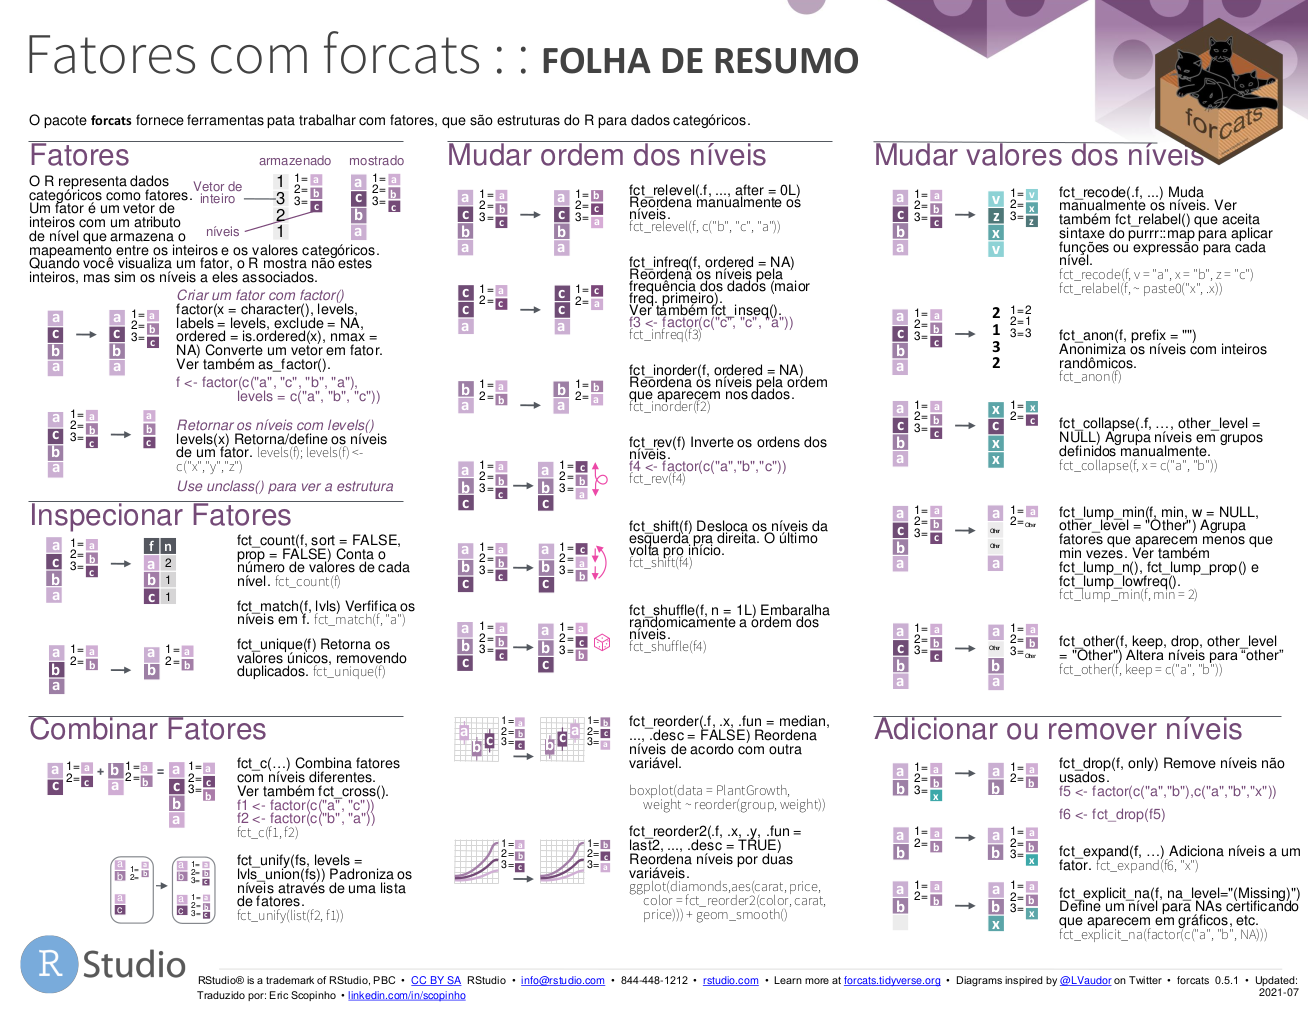
\includegraphics[width=5.39583in,height=\textheight]{Fatores/images/cs-factores-01.png}}

}

\end{figure}

\begin{center}\rule{0.5\linewidth}{0.5pt}\end{center}

\hypertarget{introduuxe7uxe3o-7}{%
\section{Introdução}\label{introduuxe7uxe3o-7}}

\textbf{Fatores} são estruturas de dados da linguagem R utilizadas para
representar \textbf{variáveis qualitativas} (categóricas). Apesar de
todo o suporte da linguagem para este tipo de dados, o pacotes forcats
facilita muito este trabalho, principalmente quando precisamos definir
níveis, alterar sua ordem, etc.

\begin{tcolorbox}[enhanced jigsaw, left=2mm, breakable, leftrule=.75mm, colback=white, colframe=quarto-callout-note-color-frame, opacityback=0, toprule=.15mm, arc=.35mm, rightrule=.15mm, bottomrule=.15mm]
\begin{minipage}[t]{5.5mm}
\textcolor{quarto-callout-note-color}{\faInfo}
\end{minipage}%
\begin{minipage}[t]{\textwidth - 5.5mm}
Para uma breve explicação do que são variáveis qualitativas, também
chamadas de categóricas, veja a seção:
\href{http://localhost:3613/Visualizacao/Visualizacao_de_dados_com_ggplot2.html\#tipos-de-vari\%C3\%A1veis}{Tipos
de Variáveis}.\end{minipage}%
\end{tcolorbox}

\hypertarget{base-de-dados-1}{%
\section{Base de Dados}\label{base-de-dados-1}}

Par os exemplos a seguir usaremos algumas tabelas já instaladas com o R
ou o pacote tidyverse como:

\hypertarget{gss_cats}{%
\subsubsection{gss\_cats}\label{gss_cats}}

\begin{Shaded}
\begin{Highlighting}[]
\NormalTok{gss\_cat}
\end{Highlighting}
\end{Shaded}

\begin{verbatim}
# A tibble: 21,483 x 9
    year marital         age race  rincome        partyid    relig denom tvhours
   <int> <fct>         <int> <fct> <fct>          <fct>      <fct> <fct>   <int>
 1  2000 Never married    26 White $8000 to 9999  Ind,near ~ Prot~ Sout~      12
 2  2000 Divorced         48 White $8000 to 9999  Not str r~ Prot~ Bapt~      NA
 3  2000 Widowed          67 White Not applicable Independe~ Prot~ No d~       2
 4  2000 Never married    39 White Not applicable Ind,near ~ Orth~ Not ~       4
 5  2000 Divorced         25 White Not applicable Not str d~ None  Not ~       1
 6  2000 Married          25 White $20000 - 24999 Strong de~ Prot~ Sout~      NA
 7  2000 Never married    36 White $25000 or more Not str r~ Chri~ Not ~       3
 8  2000 Divorced         44 White $7000 to 7999  Ind,near ~ Prot~ Luth~      NA
 9  2000 Married          44 White $25000 or more Not str d~ Prot~ Other       0
10  2000 Married          47 White $25000 or more Strong re~ Prot~ Sout~       3
# ... with 21,473 more rows
# i Use `print(n = ...)` to see more rows
\end{verbatim}

\hypertarget{diamonds}{%
\subsubsection{diamonds}\label{diamonds}}

\begin{Shaded}
\begin{Highlighting}[]
\NormalTok{diamonds  }
\end{Highlighting}
\end{Shaded}

\begin{verbatim}
# A tibble: 53,940 x 10
   carat cut       color clarity depth table price     x     y     z
   <dbl> <ord>     <ord> <ord>   <dbl> <dbl> <int> <dbl> <dbl> <dbl>
 1  0.23 Ideal     E     SI2      61.5    55   326  3.95  3.98  2.43
 2  0.21 Premium   E     SI1      59.8    61   326  3.89  3.84  2.31
 3  0.23 Good      E     VS1      56.9    65   327  4.05  4.07  2.31
 4  0.29 Premium   I     VS2      62.4    58   334  4.2   4.23  2.63
 5  0.31 Good      J     SI2      63.3    58   335  4.34  4.35  2.75
 6  0.24 Very Good J     VVS2     62.8    57   336  3.94  3.96  2.48
 7  0.24 Very Good I     VVS1     62.3    57   336  3.95  3.98  2.47
 8  0.26 Very Good H     SI1      61.9    55   337  4.07  4.11  2.53
 9  0.22 Fair      E     VS2      65.1    61   337  3.87  3.78  2.49
10  0.23 Very Good H     VS1      59.4    61   338  4     4.05  2.39
# ... with 53,930 more rows
# i Use `print(n = ...)` to see more rows
\end{verbatim}

\hypertarget{starwars}{%
\subsubsection{starwars}\label{starwars}}

\begin{Shaded}
\begin{Highlighting}[]
\NormalTok{starwars}
\end{Highlighting}
\end{Shaded}

\begin{verbatim}
# A tibble: 87 x 14
   name        height  mass hair_~1 skin_~2 eye_c~3 birth~4 sex   gender homew~5
   <chr>        <int> <dbl> <chr>   <chr>   <chr>     <dbl> <chr> <chr>  <chr>  
 1 Luke Skywa~    172    77 blond   fair    blue       19   male  mascu~ Tatooi~
 2 C-3PO          167    75 <NA>    gold    yellow    112   none  mascu~ Tatooi~
 3 R2-D2           96    32 <NA>    white,~ red        33   none  mascu~ Naboo  
 4 Darth Vader    202   136 none    white   yellow     41.9 male  mascu~ Tatooi~
 5 Leia Organa    150    49 brown   light   brown      19   fema~ femin~ Aldera~
 6 Owen Lars      178   120 brown,~ light   blue       52   male  mascu~ Tatooi~
 7 Beru White~    165    75 brown   light   blue       47   fema~ femin~ Tatooi~
 8 R5-D4           97    32 <NA>    white,~ red        NA   none  mascu~ Tatooi~
 9 Biggs Dark~    183    84 black   light   brown      24   male  mascu~ Tatooi~
10 Obi-Wan Ke~    182    77 auburn~ fair    blue-g~    57   male  mascu~ Stewjon
# ... with 77 more rows, 4 more variables: species <chr>, films <list>,
#   vehicles <list>, starships <list>, and abbreviated variable names
#   1: hair_color, 2: skin_color, 3: eye_color, 4: birth_year, 5: homeworld
# i Use `print(n = ...)` to see more rows, and `colnames()` to see all variable names
\end{verbatim}

\hypertarget{plantgrowth}{%
\subsubsection{PlantGrowth}\label{plantgrowth}}

\begin{Shaded}
\begin{Highlighting}[]
\NormalTok{PlantGrowth}
\end{Highlighting}
\end{Shaded}

\begin{verbatim}
   weight group
1    4.17  ctrl
2    5.58  ctrl
3    5.18  ctrl
4    6.11  ctrl
5    4.50  ctrl
6    4.61  ctrl
7    5.17  ctrl
8    4.53  ctrl
9    5.33  ctrl
10   5.14  ctrl
11   4.81  trt1
12   4.17  trt1
13   4.41  trt1
14   3.59  trt1
15   5.87  trt1
16   3.83  trt1
17   6.03  trt1
18   4.89  trt1
19   4.32  trt1
20   4.69  trt1
21   6.31  trt2
22   5.12  trt2
23   5.54  trt2
24   5.50  trt2
25   5.37  trt2
26   5.29  trt2
27   4.92  trt2
28   6.15  trt2
29   5.80  trt2
30   5.26  trt2
\end{verbatim}

Note que as variáveis do tipo \textbf{fator} são marcadas como
``\textbf{fct}'' nas tabelas acima.

\hypertarget{fatores}{%
\section{Fatores}\label{fatores}}

A linguagem R representa \textbf{dados categóricos} através de um tipo
de dados chamado \textbf{Fator} (factor). Um fator é um vetor de
inteiros com um atributo de \textbf{nível} (level) associado à ele. Este
nível armazena um conjunto de mapeamentos entre o inteiro e o valor
categórico. Quando você visualiza um fator, o R não mostra os inteiros,
mas sim, os níveis associados à eles.

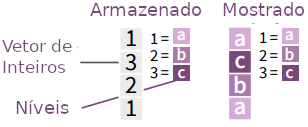
\includegraphics[width=2.63542in,height=\textheight]{Fatores/images/factors-01.png}

\hypertarget{factor}{%
\subsubsection{factor}\label{factor}}

Use esta função para criar um fator.

\begin{Shaded}
\begin{Highlighting}[]
\NormalTok{f }\OtherTok{\textless{}{-}} \FunctionTok{factor}\NormalTok{(}\FunctionTok{c}\NormalTok{(}\StringTok{"a"}\NormalTok{, }\StringTok{"c"}\NormalTok{, }\StringTok{"b"}\NormalTok{, }\StringTok{"a"}\NormalTok{), }\AttributeTok{levels =} \FunctionTok{c}\NormalTok{(}\StringTok{"a"}\NormalTok{, }\StringTok{"b"}\NormalTok{, }\StringTok{"c"}\NormalTok{))}
\NormalTok{f}
\end{Highlighting}
\end{Shaded}

\begin{verbatim}
[1] a c b a
Levels: a b c
\end{verbatim}

No exemplos acima, criamos um fator à partir de um vetor (a,b,c,a) e
definimos os níveis 1, 2 e 3 como ``a,b,c''.

\begin{tcolorbox}[enhanced jigsaw, rightrule=.15mm, arc=.35mm, coltitle=black, colframe=quarto-callout-note-color-frame, opacityback=0, toprule=.15mm, left=2mm, breakable, colback=white, bottomtitle=1mm, leftrule=.75mm, title=\textcolor{quarto-callout-note-color}{\faInfo}\hspace{0.5em}{Nota}, colbacktitle=quarto-callout-note-color!10!white, titlerule=0mm, bottomrule=.15mm, toptitle=1mm, opacitybacktitle=0.6]

Se os \textbf{níveis} de um fator \textbf{não forem especificados}, o R
irá pegar os caracteres únicos do vetor e colocá-los em ordem
alfabética.

\begin{Shaded}
\begin{Highlighting}[]
\NormalTok{f }\OtherTok{\textless{}{-}} \FunctionTok{factor}\NormalTok{(}\FunctionTok{c}\NormalTok{(}\StringTok{"a"}\NormalTok{, }\StringTok{"c"}\NormalTok{, }\StringTok{"b"}\NormalTok{, }\StringTok{"a"}\NormalTok{))}
\NormalTok{f}
\end{Highlighting}
\end{Shaded}

\begin{verbatim}
[1] a c b a
Levels: a b c
\end{verbatim}

\end{tcolorbox}

\hypertarget{as_fator}{%
\subsubsection{as\_fator}\label{as_fator}}

Podemos também converter um outro tipo de dado para fator utilzando a
função as\_factor.

\begin{Shaded}
\begin{Highlighting}[]
\NormalTok{vetor }\OtherTok{\textless{}{-}} \FunctionTok{c}\NormalTok{(}\StringTok{"a"}\NormalTok{, }\StringTok{"b"}\NormalTok{, }\StringTok{"c"}\NormalTok{, }\StringTok{"a"}\NormalTok{)}
\FunctionTok{as\_factor}\NormalTok{(vetor)}
\end{Highlighting}
\end{Shaded}

\begin{verbatim}
[1] a b c a
Levels: a b c
\end{verbatim}

\hypertarget{levels}{%
\subsubsection{levels}\label{levels}}

Use para retornar ou definir os níveis de um fator.

\begin{Shaded}
\begin{Highlighting}[]
\CommentTok{\# para retornar os níveis:}
\FunctionTok{levels}\NormalTok{(f)}
\end{Highlighting}
\end{Shaded}

\begin{verbatim}
[1] "a" "b" "c"
\end{verbatim}

\begin{Shaded}
\begin{Highlighting}[]
\CommentTok{\# Para definir os níveis:}
\FunctionTok{levels}\NormalTok{ (f) }\OtherTok{\textless{}{-}} \FunctionTok{c}\NormalTok{(}\StringTok{"x"}\NormalTok{, }\StringTok{"y"}\NormalTok{, }\StringTok{"z"}\NormalTok{)}
\NormalTok{f}
\end{Highlighting}
\end{Shaded}

\begin{verbatim}
[1] x z y x
Levels: x y z
\end{verbatim}

\begin{Shaded}
\begin{Highlighting}[]
\FunctionTok{levels}\NormalTok{ (f) }\OtherTok{\textless{}{-}} \FunctionTok{c}\NormalTok{(}\StringTok{"a"}\NormalTok{, }\StringTok{"b"}\NormalTok{, }\StringTok{"c"}\NormalTok{)}
\NormalTok{f}
\end{Highlighting}
\end{Shaded}

\begin{verbatim}
[1] a c b a
Levels: a b c
\end{verbatim}

Veja outro exemplo:

\begin{Shaded}
\begin{Highlighting}[]
\NormalTok{f\_meses }\OtherTok{\textless{}{-}} \FunctionTok{factor}\NormalTok{(}\FunctionTok{c}\NormalTok{(}\StringTok{"Jan"}\NormalTok{, }\StringTok{"Fev"}\NormalTok{, }\StringTok{"Mar"}\NormalTok{, }\StringTok{"Abr"}\NormalTok{))}
\NormalTok{f\_meses}
\end{Highlighting}
\end{Shaded}

\begin{verbatim}
[1] Jan Fev Mar Abr
Levels: Abr Fev Jan Mar
\end{verbatim}

Como não definimos os níveis do factor, ele colocou em ordem alfabética
à partir dos valores definidos.

Para colocar os nível na ordem dos meses, podemos fazer:

\begin{Shaded}
\begin{Highlighting}[]
\NormalTok{meses }\OtherTok{\textless{}{-}} \FunctionTok{c}\NormalTok{(}\StringTok{"Jan"}\NormalTok{, }\StringTok{"Fev"}\NormalTok{, }\StringTok{"Mar"}\NormalTok{, }\StringTok{"Abr"}\NormalTok{)}
\FunctionTok{levels}\NormalTok{ (f\_meses) }\OtherTok{\textless{}{-}}\NormalTok{ meses}
\NormalTok{f\_meses}
\end{Highlighting}
\end{Shaded}

\begin{verbatim}
[1] Mar Fev Abr Jan
Levels: Jan Fev Mar Abr
\end{verbatim}

\begin{tcolorbox}[enhanced jigsaw, rightrule=.15mm, arc=.35mm, coltitle=black, colframe=quarto-callout-tip-color-frame, opacityback=0, toprule=.15mm, left=2mm, breakable, colback=white, bottomtitle=1mm, leftrule=.75mm, title=\textcolor{quarto-callout-tip-color}{\faLightbulb}\hspace{0.5em}{Dica}, colbacktitle=quarto-callout-tip-color!10!white, titlerule=0mm, bottomrule=.15mm, toptitle=1mm, opacitybacktitle=0.6]
Estas configurações adequadas dos meses, são importantes em diversas
ocasiões, dentre elas, quando precisamos gerar um gráfico com a
variáveis categórica no GGPLOT, pois este leva em consideração os níveis
para definir a ordem no gráfico.
\end{tcolorbox}

\hypertarget{inspecionando-fatores}{%
\section{Inspecionando Fatores}\label{inspecionando-fatores}}

\hypertarget{fct_count}{%
\subsubsection{fct\_count}\label{fct_count}}

Use para contar os valores de cada nível.

\begin{Shaded}
\begin{Highlighting}[]
\FunctionTok{fct\_count}\NormalTok{(f)}
\end{Highlighting}
\end{Shaded}

\begin{verbatim}
# A tibble: 3 x 2
  f         n
  <fct> <int>
1 a         2
2 b         1
3 c         1
\end{verbatim}

\hypertarget{fct_match}{%
\subsubsection{fct\_match}\label{fct_match}}

Use para encontrar níveis.

\begin{Shaded}
\begin{Highlighting}[]
\FunctionTok{fct\_match}\NormalTok{(f, }\StringTok{"a"}\NormalTok{)}
\end{Highlighting}
\end{Shaded}

\begin{verbatim}
[1]  TRUE FALSE FALSE  TRUE
\end{verbatim}

\hypertarget{fct_unique}{%
\subsubsection{fct\_unique}\label{fct_unique}}

Use para retornar valores únicos de um fator, removendo os duplicados.

\begin{Shaded}
\begin{Highlighting}[]
\FunctionTok{fct\_unique}\NormalTok{(f)}
\end{Highlighting}
\end{Shaded}

\begin{verbatim}
[1] a b c
Levels: a b c
\end{verbatim}

\hypertarget{combinando-fatores}{%
\section{Combinando Fatores}\label{combinando-fatores}}

\hypertarget{fct_c}{%
\subsubsection{fct\_c}\label{fct_c}}

Use para combinar fatores com níveis diferentes.

\begin{Shaded}
\begin{Highlighting}[]
\NormalTok{f1 }\OtherTok{\textless{}{-}} \FunctionTok{factor}\NormalTok{(}\FunctionTok{c}\NormalTok{(}\StringTok{"a"}\NormalTok{, }\StringTok{"b"}\NormalTok{, }\StringTok{"c"}\NormalTok{))}
\NormalTok{f2 }\OtherTok{\textless{}{-}} \FunctionTok{factor}\NormalTok{(}\FunctionTok{c}\NormalTok{(}\StringTok{"b"}\NormalTok{, }\StringTok{"a"}\NormalTok{))}
\end{Highlighting}
\end{Shaded}

\begin{Shaded}
\begin{Highlighting}[]
\NormalTok{f1}
\end{Highlighting}
\end{Shaded}

\begin{verbatim}
[1] a b c
Levels: a b c
\end{verbatim}

\begin{Shaded}
\begin{Highlighting}[]
\NormalTok{f2}
\end{Highlighting}
\end{Shaded}

\begin{verbatim}
[1] b a
Levels: a b
\end{verbatim}

\begin{Shaded}
\begin{Highlighting}[]
\FunctionTok{fct\_c}\NormalTok{(f1,f2)}
\end{Highlighting}
\end{Shaded}

\begin{verbatim}
[1] a b c b a
Levels: a b c
\end{verbatim}

\begin{tcolorbox}[enhanced jigsaw, rightrule=.15mm, arc=.35mm, coltitle=black, colframe=quarto-callout-tip-color-frame, opacityback=0, toprule=.15mm, left=2mm, breakable, colback=white, bottomtitle=1mm, leftrule=.75mm, title=\textcolor{quarto-callout-tip-color}{\faLightbulb}\hspace{0.5em}{Dica}, colbacktitle=quarto-callout-tip-color!10!white, titlerule=0mm, bottomrule=.15mm, toptitle=1mm, opacitybacktitle=0.6]
Use \textbf{fct\_cross}() para criar um fator à partir de dois ou mais
fatores, gerando níveis para todas as combinações possíveis.
\end{tcolorbox}

\hypertarget{fct_unify}{%
\subsubsection{fct\_unify}\label{fct_unify}}

Use para padronizar os níveis à partir de uma lista de fatores.

\begin{Shaded}
\begin{Highlighting}[]
\FunctionTok{list}\NormalTok{(f1, f2)}
\end{Highlighting}
\end{Shaded}

\begin{verbatim}
[[1]]
[1] a b c
Levels: a b c

[[2]]
[1] b a
Levels: a b
\end{verbatim}

\begin{Shaded}
\begin{Highlighting}[]
\FunctionTok{fct\_unify}\NormalTok{(}\FunctionTok{list}\NormalTok{(f2, f1))}
\end{Highlighting}
\end{Shaded}

\begin{verbatim}
[[1]]
[1] b a
Levels: a b c

[[2]]
[1] a b c
Levels: a b c
\end{verbatim}

Veja que no exemplo acima, os níveis de ambas as listas agora possuem os
mesmos valores.

\hypertarget{mudando-as-ordens-dos-nuxedveis}{%
\section{Mudando as ordens dos
Níveis}\label{mudando-as-ordens-dos-nuxedveis}}

\hypertarget{fct_relevel}{%
\subsubsection{fct\_relevel}\label{fct_relevel}}

Use para redefinir a \textbf{ordem dos níveis}.

\begin{Shaded}
\begin{Highlighting}[]
\FunctionTok{fct\_relevel}\NormalTok{(f, }\FunctionTok{c}\NormalTok{(}\StringTok{"b"}\NormalTok{, }\StringTok{"c"}\NormalTok{, }\StringTok{"a"}\NormalTok{))}
\end{Highlighting}
\end{Shaded}

\begin{verbatim}
[1] a c b a
Levels: b c a
\end{verbatim}

\hypertarget{fct_reorder}{%
\subsubsection{fct\_reorder}\label{fct_reorder}}

Use para definir a \textbf{ordem dos níveis}, baseadas em \textbf{outra
variável}. Ou seja, ela ordena os níveis de acordo com esta outra
variável. Para explicar melhor, vamos criar um data frame (df) e definir
a variavel color com fator:

\begin{Shaded}
\begin{Highlighting}[]
\NormalTok{df }\OtherTok{\textless{}{-}}\NormalTok{ tibble}\SpecialCharTok{::}\FunctionTok{tribble}\NormalTok{(}
  \SpecialCharTok{\textasciitilde{}}\NormalTok{color,     }\SpecialCharTok{\textasciitilde{}}\NormalTok{a, }\SpecialCharTok{\textasciitilde{}}\NormalTok{b,}
  \StringTok{"blue"}\NormalTok{,      }\DecValTok{1}\NormalTok{,  }\DecValTok{2}\NormalTok{,}
  \StringTok{"green"}\NormalTok{,     }\DecValTok{6}\NormalTok{,  }\DecValTok{2}\NormalTok{,}
  \StringTok{"purple"}\NormalTok{,    }\DecValTok{3}\NormalTok{,  }\DecValTok{3}\NormalTok{,}
  \StringTok{"red"}\NormalTok{,       }\DecValTok{2}\NormalTok{,  }\DecValTok{3}\NormalTok{,}
  \StringTok{"yellow"}\NormalTok{,    }\DecValTok{5}\NormalTok{,  }\DecValTok{1}
\NormalTok{)}

\NormalTok{df}\SpecialCharTok{$}\NormalTok{color }\OtherTok{\textless{}{-}} \FunctionTok{factor}\NormalTok{(df}\SpecialCharTok{$}\NormalTok{color)}
\NormalTok{df}
\end{Highlighting}
\end{Shaded}

\begin{verbatim}
# A tibble: 5 x 3
  color      a     b
  <fct>  <dbl> <dbl>
1 blue       1     2
2 green      6     2
3 purple     3     3
4 red        2     3
5 yellow     5     1
\end{verbatim}

Agora, vamos analisar os níveis de color e depois utilizar a função
fct\_order() para reordenar este níveis de acordo com os números
definidos na variável ``a''.

\begin{Shaded}
\begin{Highlighting}[]
\NormalTok{df}\SpecialCharTok{$}\NormalTok{color}
\end{Highlighting}
\end{Shaded}

\begin{verbatim}
[1] blue   green  purple red    yellow
Levels: blue green purple red yellow
\end{verbatim}

\begin{Shaded}
\begin{Highlighting}[]
\FunctionTok{fct\_reorder}\NormalTok{(df}\SpecialCharTok{$}\NormalTok{color, df}\SpecialCharTok{$}\NormalTok{a)}
\end{Highlighting}
\end{Shaded}

\begin{verbatim}
[1] blue   green  purple red    yellow
Levels: blue red purple yellow green
\end{verbatim}

No próximo exemplo, utilzamos a função \textbf{fct\_reorder} para
ordenar os níveis da variável ``\textbf{group}'' em função dos valores
da variável ``\textbf{weight}''.

Veja como fica um gráfico de boxplot, sem e depois com os níveis
reordenados:

\begin{Shaded}
\begin{Highlighting}[]
\CommentTok{\#Sem ftc\_reorder}
\NormalTok{PlantGrowth }\SpecialCharTok{|\textgreater{}} 
  \FunctionTok{ggplot}\NormalTok{(}\FunctionTok{aes}\NormalTok{(group , weight, }\AttributeTok{fill =}\NormalTok{ group)) }\SpecialCharTok{+} 
  \FunctionTok{geom\_boxplot}\NormalTok{()}
\CommentTok{\#Com fct\_reorder}
\NormalTok{PlantGrowth }\SpecialCharTok{|\textgreater{}} 
  \FunctionTok{ggplot}\NormalTok{(}\FunctionTok{aes}\NormalTok{(}\FunctionTok{fct\_reorder}\NormalTok{(group, weight) , weight, }\AttributeTok{fill =}\NormalTok{ group)) }\SpecialCharTok{+} 
  \FunctionTok{geom\_boxplot}\NormalTok{()}
\end{Highlighting}
\end{Shaded}

\begin{figure}

\begin{minipage}[t]{0.50\linewidth}

{\centering 

\raisebox{-\height}{

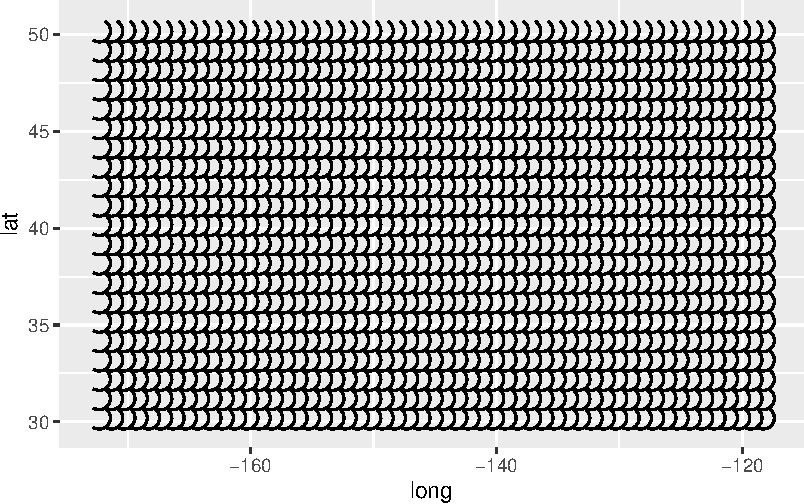
\includegraphics{Fatores/Fatores_com_forcats_files/figure-pdf/unnamed-chunk-24-1.pdf}

}

}

\end{minipage}%
%
\begin{minipage}[t]{0.50\linewidth}

{\centering 

\raisebox{-\height}{

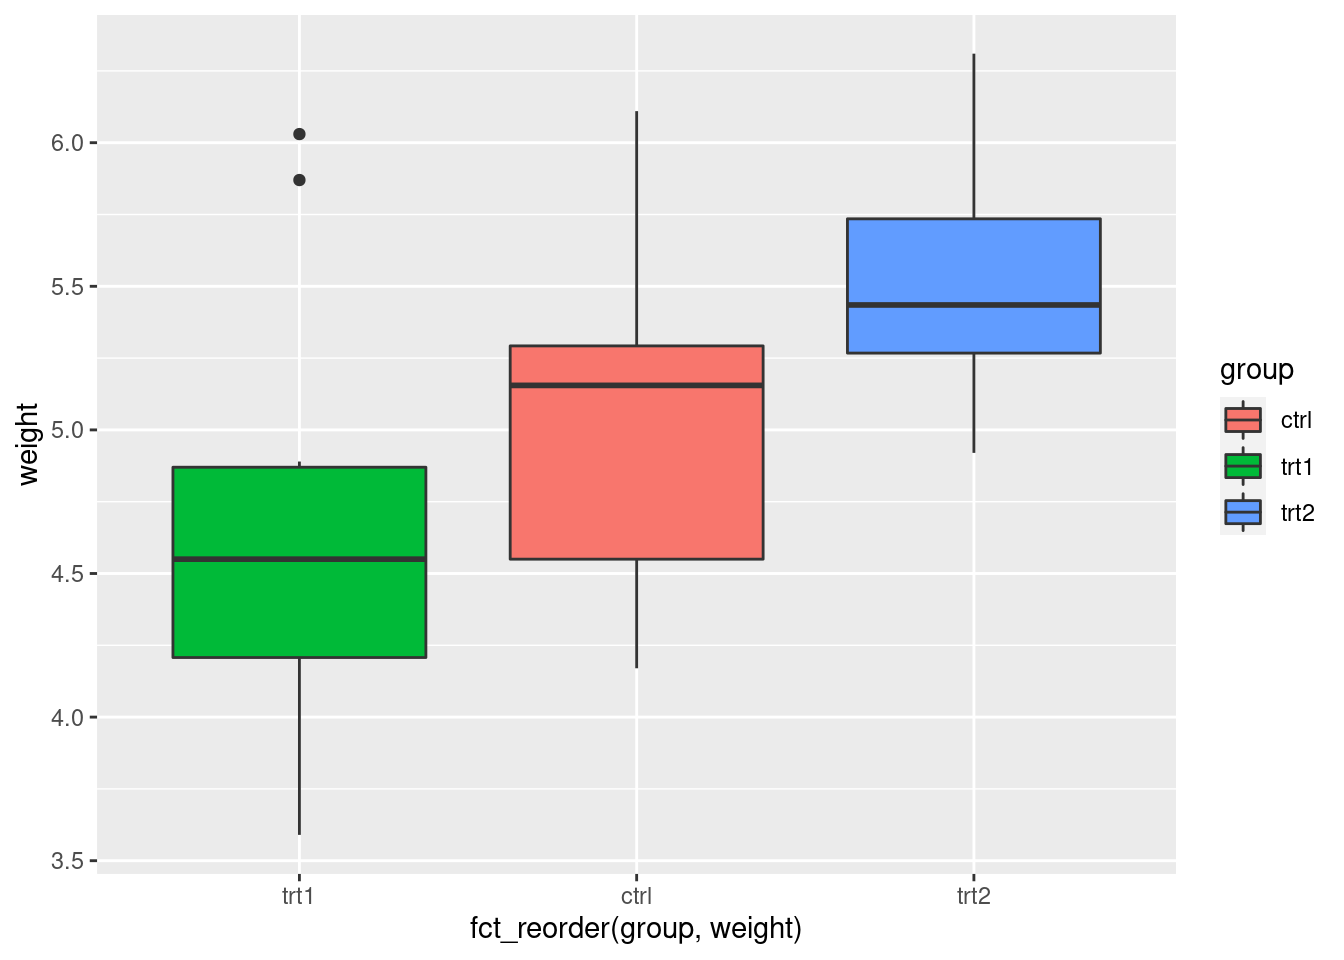
\includegraphics{Fatores/Fatores_com_forcats_files/figure-pdf/unnamed-chunk-24-2.pdf}

}

}

\end{minipage}%

\end{figure}

\hypertarget{fct_reorder2}{%
\subsubsection{fct\_reorder2}\label{fct_reorder2}}

Use para definir a \textbf{ordem do fator com base nos valores}.

Ainda usando o data frame (df) criado visto na função fct\_reorder,
vejamos a diferença para utilizar o fct\_reorder2(). Neste caso,
utilizamos duas variáveis (a e b) para reordenar a variável color.

\begin{Shaded}
\begin{Highlighting}[]
\NormalTok{df }
\FunctionTok{fct\_reorder2}\NormalTok{(df}\SpecialCharTok{$}\NormalTok{color, df}\SpecialCharTok{$}\NormalTok{a, df}\SpecialCharTok{$}\NormalTok{b)}
\end{Highlighting}
\end{Shaded}

\begin{figure}

\begin{minipage}[t]{\linewidth}

{\centering 

\begin{verbatim}
# A tibble: 5 x 3
  color      a     b
  <fct>  <dbl> <dbl>
1 blue       1     2
2 green      6     2
3 purple     3     3
4 red        2     3
5 yellow     5     1
\end{verbatim}

}

\end{minipage}%
\newline
\begin{minipage}[t]{\linewidth}

{\centering 

\begin{verbatim}
[1] blue   green  purple red    yellow
Levels: purple red blue green yellow
\end{verbatim}

}

\end{minipage}%

\end{figure}

Em geral, utilzamos este tipo de reordenação de uma variável fator de
acordo com duas variáveis, quando queremos visualizar uma estética não
posicional em um gráfico, como color, size, fill, etc.

\begin{Shaded}
\begin{Highlighting}[]
\CommentTok{\# Sem a reordenação de nível com fct\_reorder2}
\NormalTok{diamonds }\SpecialCharTok{|\textgreater{}} 
  \FunctionTok{ggplot}\NormalTok{(}\FunctionTok{aes}\NormalTok{(carat, }
\NormalTok{             price, }\AttributeTok{color =}\NormalTok{ color)) }\SpecialCharTok{+} 
             \CommentTok{\#color = fct\_reorder2 (color, carat, price))) + }
  \FunctionTok{geom\_smooth}\NormalTok{()}
\CommentTok{\# Com a reordenação de nível com fct\_reorder2}
\NormalTok{diamonds }\SpecialCharTok{|\textgreater{}} 
  \FunctionTok{ggplot}\NormalTok{(}\FunctionTok{aes}\NormalTok{(carat, }
\NormalTok{             price, }
             \AttributeTok{color =} \FunctionTok{fct\_reorder2}\NormalTok{ (color, carat, price))) }\SpecialCharTok{+} 
  \FunctionTok{labs}\NormalTok{(}\AttributeTok{color =} \StringTok{"color"}\NormalTok{)}\SpecialCharTok{+}
  \FunctionTok{geom\_smooth}\NormalTok{()}
\end{Highlighting}
\end{Shaded}

\begin{figure}

\begin{minipage}[t]{0.50\linewidth}

{\centering 

\raisebox{-\height}{

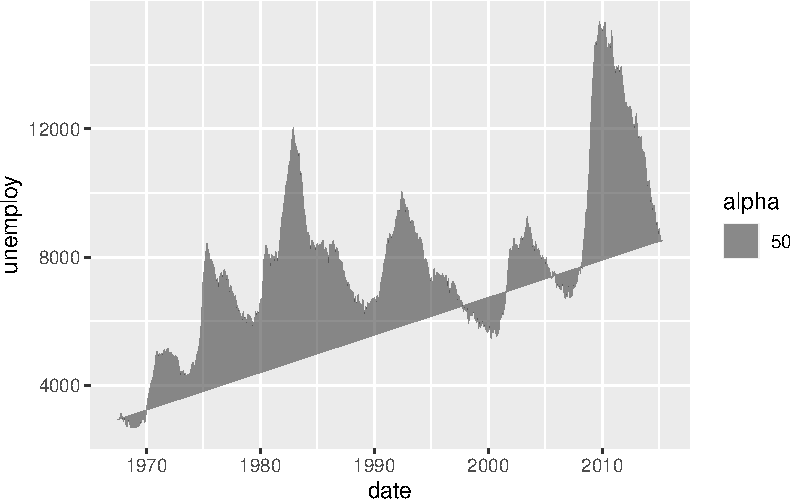
\includegraphics{Fatores/Fatores_com_forcats_files/figure-pdf/unnamed-chunk-26-1.pdf}

}

}

\end{minipage}%
%
\begin{minipage}[t]{0.50\linewidth}

{\centering 

\raisebox{-\height}{

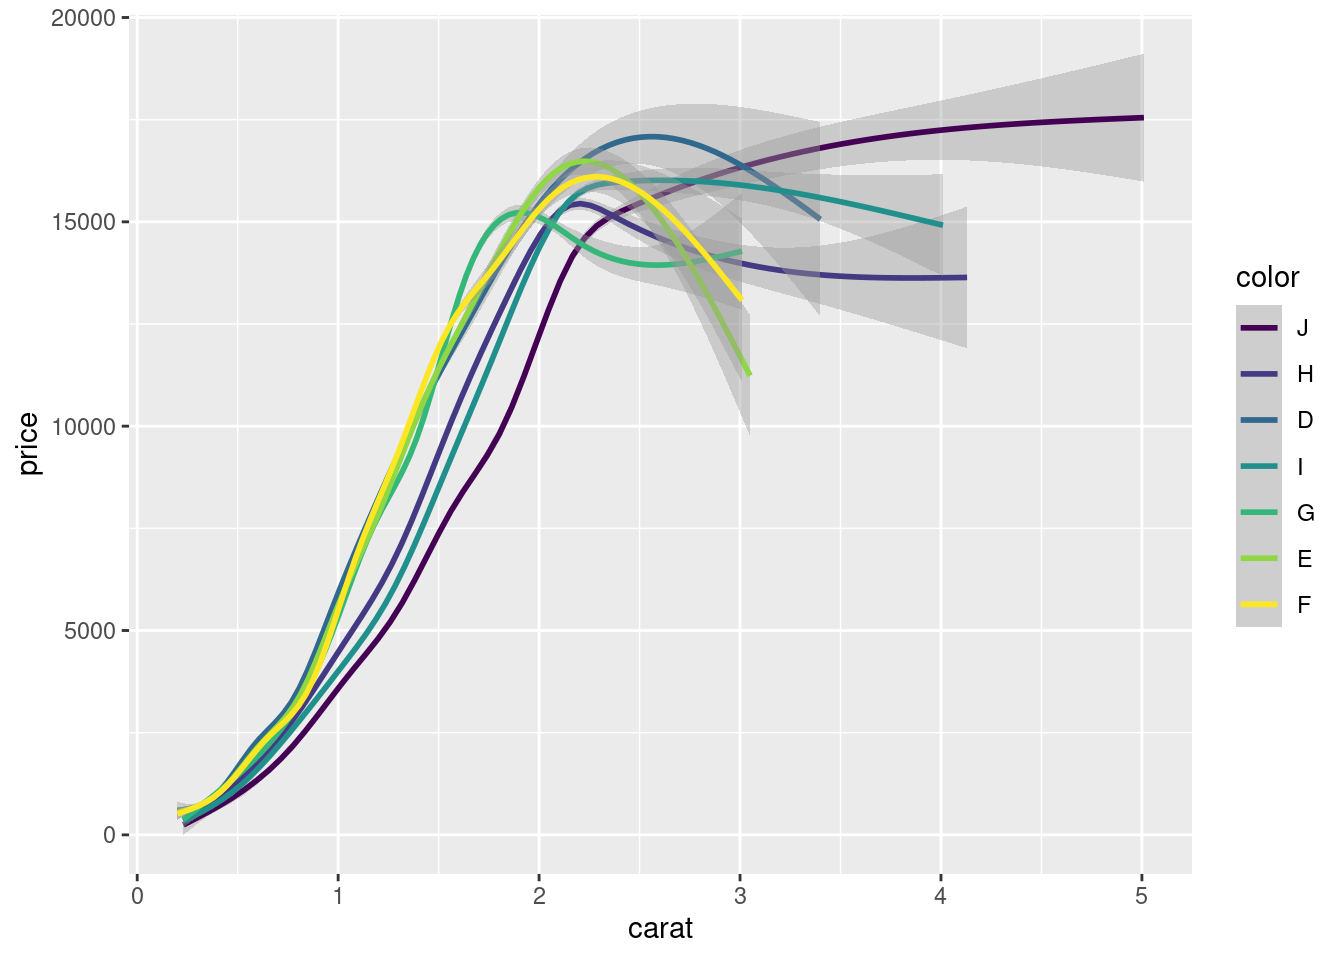
\includegraphics{Fatores/Fatores_com_forcats_files/figure-pdf/unnamed-chunk-26-2.pdf}

}

}

\end{minipage}%

\end{figure}

\hypertarget{fct_infreq}{%
\subsubsection{fct\_infreq}\label{fct_infreq}}

Use para reordenar os níveis de um fator, pela primeira ordem de
\textbf{frequência} dos dados. Maior frequência aparece em primeiro.

\begin{Shaded}
\begin{Highlighting}[]
\NormalTok{f3 }\OtherTok{\textless{}{-}} \FunctionTok{factor}\NormalTok{(}\FunctionTok{c}\NormalTok{(}\StringTok{"c"}\NormalTok{, }\StringTok{"c"}\NormalTok{, }\StringTok{"a"}\NormalTok{))}
\FunctionTok{fct\_infreq}\NormalTok{(f3)}
\end{Highlighting}
\end{Shaded}

\begin{verbatim}
[1] c c a
Levels: c a
\end{verbatim}

\begin{tcolorbox}[enhanced jigsaw, rightrule=.15mm, arc=.35mm, coltitle=black, colframe=quarto-callout-tip-color-frame, opacityback=0, toprule=.15mm, left=2mm, breakable, colback=white, bottomtitle=1mm, leftrule=.75mm, title=\textcolor{quarto-callout-tip-color}{\faLightbulb}\hspace{0.5em}{Dica}, colbacktitle=quarto-callout-tip-color!10!white, titlerule=0mm, bottomrule=.15mm, toptitle=1mm, opacitybacktitle=0.6]
Se quiser reordenar os níveis usando os valores numéricos dos níveis,
use \textbf{fct\_inseq}().
\end{tcolorbox}

\hypertarget{fct_inorder}{%
\subsubsection{fct\_inorder}\label{fct_inorder}}

Use para \textbf{reordenar} os níveis de um fator, pela \textbf{ordem}
\textbf{de aparecimento} dos dados na linhas.

\begin{Shaded}
\begin{Highlighting}[]
\NormalTok{f2}
\end{Highlighting}
\end{Shaded}

\begin{verbatim}
[1] b a
Levels: a b
\end{verbatim}

\begin{Shaded}
\begin{Highlighting}[]
\FunctionTok{fct\_inorder}\NormalTok{(f2)}
\end{Highlighting}
\end{Shaded}

\begin{verbatim}
[1] b a
Levels: b a
\end{verbatim}

\hypertarget{fct_rev}{%
\subsubsection{fct\_rev}\label{fct_rev}}

Use para \textbf{inverter} a ordem dos níveis de um vetor.

\begin{Shaded}
\begin{Highlighting}[]
\NormalTok{f4 }\OtherTok{\textless{}{-}} \FunctionTok{factor}\NormalTok{(}\FunctionTok{c}\NormalTok{(}\StringTok{"a"}\NormalTok{,}\StringTok{"b"}\NormalTok{,}\StringTok{"c"}\NormalTok{))}
\NormalTok{f4}
\end{Highlighting}
\end{Shaded}

\begin{verbatim}
[1] a b c
Levels: a b c
\end{verbatim}

\begin{Shaded}
\begin{Highlighting}[]
\FunctionTok{fct\_rev}\NormalTok{(f4)}
\end{Highlighting}
\end{Shaded}

\begin{verbatim}
[1] a b c
Levels: c b a
\end{verbatim}

\hypertarget{fct_shift}{%
\subsubsection{fct\_shift}\label{fct_shift}}

Use para \textbf{deslocar} a ordem dos níveis de um fator. Use o
argumento n= para deslocar n casas.

\begin{Shaded}
\begin{Highlighting}[]
\NormalTok{f}
\end{Highlighting}
\end{Shaded}

\begin{verbatim}
[1] a c b a
Levels: a b c
\end{verbatim}

\begin{Shaded}
\begin{Highlighting}[]
\FunctionTok{fct\_shift}\NormalTok{(f)}
\end{Highlighting}
\end{Shaded}

\begin{verbatim}
[1] a c b a
Levels: b c a
\end{verbatim}

\hypertarget{fct_shuffle}{%
\subsubsection{fct\_shuffle}\label{fct_shuffle}}

Use para embaralhar randomicamente dos níveis de um fator.

\begin{Shaded}
\begin{Highlighting}[]
\FunctionTok{fct\_shuffle}\NormalTok{(f4)}
\end{Highlighting}
\end{Shaded}

\begin{verbatim}
[1] a b c
Levels: b a c
\end{verbatim}

\begin{Shaded}
\begin{Highlighting}[]
\FunctionTok{fct\_shuffle}\NormalTok{(f4)}
\end{Highlighting}
\end{Shaded}

\begin{verbatim}
[1] a b c
Levels: a c b
\end{verbatim}

\hypertarget{mudando-os-valores-dos-nuxedveis}{%
\section{Mudando os valores dos
Níveis}\label{mudando-os-valores-dos-nuxedveis}}

\hypertarget{fct_recode}{%
\subsubsection{fct\_recode}\label{fct_recode}}

Use para mudar manualmente os valores dos níveis de um fator.

\begin{Shaded}
\begin{Highlighting}[]
\NormalTok{f}
\end{Highlighting}
\end{Shaded}

\begin{verbatim}
[1] a c b a
Levels: a b c
\end{verbatim}

\begin{Shaded}
\begin{Highlighting}[]
\FunctionTok{fct\_recode}\NormalTok{(f, }\AttributeTok{v =} \StringTok{"a"}\NormalTok{, }\AttributeTok{x =} \StringTok{"b"}\NormalTok{, }\AttributeTok{z =} \StringTok{"c"}\NormalTok{)}
\end{Highlighting}
\end{Shaded}

\begin{verbatim}
[1] v z x v
Levels: v x z
\end{verbatim}

\hypertarget{fct_relabel}{%
\subsubsection{fct\_relabel}\label{fct_relabel}}

Use para mudar \textbf{programaticamente} os nomes. Esta função aceita a
sintaxe de funções do pacote purrr. Pode-se usar expressões regulares,
etc.

\begin{Shaded}
\begin{Highlighting}[]
\FunctionTok{fct\_relabel}\NormalTok{(f, }\SpecialCharTok{\textasciitilde{}} \FunctionTok{paste0}\NormalTok{(}\StringTok{"x"}\NormalTok{, .x))}
\end{Highlighting}
\end{Shaded}

\begin{verbatim}
[1] xa xc xb xa
Levels: xa xb xc
\end{verbatim}

\hypertarget{fct_anon}{%
\subsubsection{fct\_anon}\label{fct_anon}}

Use para anonimizar os valores dos níveis com números randômicos.

\begin{Shaded}
\begin{Highlighting}[]
\FunctionTok{fct\_anon}\NormalTok{(f)}
\end{Highlighting}
\end{Shaded}

\begin{verbatim}
[1] 2 3 1 2
Levels: 1 2 3
\end{verbatim}

\hypertarget{fct_collapse}{%
\subsubsection{fct\_collapse}\label{fct_collapse}}

Use para \textbf{agrupar} níveis definindo grupos \textbf{manualmente}.

\begin{Shaded}
\begin{Highlighting}[]
\NormalTok{f}
\end{Highlighting}
\end{Shaded}

\begin{verbatim}
[1] a c b a
Levels: a b c
\end{verbatim}

\begin{Shaded}
\begin{Highlighting}[]
\FunctionTok{fct\_collapse}\NormalTok{(f, }\AttributeTok{x =} \FunctionTok{c}\NormalTok{(}\StringTok{"a"}\NormalTok{, }\StringTok{"b"}\NormalTok{))}
\end{Highlighting}
\end{Shaded}

\begin{verbatim}
[1] x c x x
Levels: x c
\end{verbatim}

\hypertarget{fct_lump_min}{%
\subsubsection{fct\_lump\_min}\label{fct_lump_min}}

Use para agrupar em um único grupo os níveis de um fator que aparecem
menos que n vezes.

\begin{Shaded}
\begin{Highlighting}[]
\NormalTok{f}
\end{Highlighting}
\end{Shaded}

\begin{verbatim}
[1] a c b a
Levels: a b c
\end{verbatim}

\begin{Shaded}
\begin{Highlighting}[]
\FunctionTok{fct\_lump\_min}\NormalTok{(f, }\AttributeTok{min =} \DecValTok{2}\NormalTok{)}
\end{Highlighting}
\end{Shaded}

\begin{verbatim}
[1] a     Other Other a    
Levels: a Other
\end{verbatim}

\begin{tcolorbox}[enhanced jigsaw, rightrule=.15mm, arc=.35mm, coltitle=black, colframe=quarto-callout-tip-color-frame, opacityback=0, toprule=.15mm, left=2mm, breakable, colback=white, bottomtitle=1mm, leftrule=.75mm, title=\textcolor{quarto-callout-tip-color}{\faLightbulb}\hspace{0.5em}{Dica}, colbacktitle=quarto-callout-tip-color!10!white, titlerule=0mm, bottomrule=.15mm, toptitle=1mm, opacitybacktitle=0.6]
Use o argumento \textbf{other\_level=} para dar um nome defierente de
``Other'' quando precisar.
\end{tcolorbox}

Este grupo de funções tem também:

\textbf{fct\_prop}: Para agrupar em um único grupo valores com
proporções menores que n\% vezes.

\textbf{fct\_lowfreq}: Para agrupar em um único grupo valores com as
menores frequências, garantindo que o grupo ``other'' tem o menor nível.

\textbf{fct\_lump\_n}: Para agrupar em um único grupo valores exceto
aqueles com o número de frequência maior que o argumento n=.

Veja mais um exemplo, mesclando vários conceitos que vimos até aqui, mas
com foco nas funções \textbf{fct\_lummp\_n}() e \textbf{fct\_shift}():

\begin{Shaded}
\begin{Highlighting}[]
\NormalTok{ starwars }\SpecialCharTok{|\textgreater{}} 
   \FunctionTok{drop\_na}\NormalTok{()}\SpecialCharTok{|\textgreater{}} 
   \FunctionTok{ggplot}\NormalTok{(}\FunctionTok{aes}\NormalTok{(}
     \AttributeTok{fill =} \FunctionTok{fct\_lump\_n}\NormalTok{(homeworld, }\AttributeTok{n =} \DecValTok{3}\NormalTok{),}
     \AttributeTok{x =} \FunctionTok{fct\_shift}\NormalTok{(}
                \FunctionTok{fct\_lump\_n}\NormalTok{(homeworld, }\AttributeTok{n =} \DecValTok{3}\NormalTok{,}\AttributeTok{other\_level =} \StringTok{"Outros"}\NormalTok{), }
                \AttributeTok{n =} \SpecialCharTok{{-}}\NormalTok{1L))) }\SpecialCharTok{+}
   \FunctionTok{scale\_fill\_brewer}\NormalTok{(}\AttributeTok{palette =} \StringTok{"Dark2"}\NormalTok{, }\AttributeTok{guide =} \StringTok{"none"}\NormalTok{) }\SpecialCharTok{+} 
   \FunctionTok{geom\_bar}\NormalTok{()}\SpecialCharTok{+}
   \FunctionTok{geom\_label}\NormalTok{(}\AttributeTok{stat =} \StringTok{"count"}\NormalTok{, }\FunctionTok{aes}\NormalTok{(}\AttributeTok{label =} \FunctionTok{after\_stat}\NormalTok{(count)))}\SpecialCharTok{+}
   \FunctionTok{labs}\NormalTok{(}\AttributeTok{x =}\StringTok{"Mundo"}\NormalTok{, }\AttributeTok{y=}\StringTok{"Qtd de Personagens"}\NormalTok{) }\SpecialCharTok{+} 
   \FunctionTok{coord\_flip}\NormalTok{()}
\end{Highlighting}
\end{Shaded}

\begin{figure}[H]

{\centering 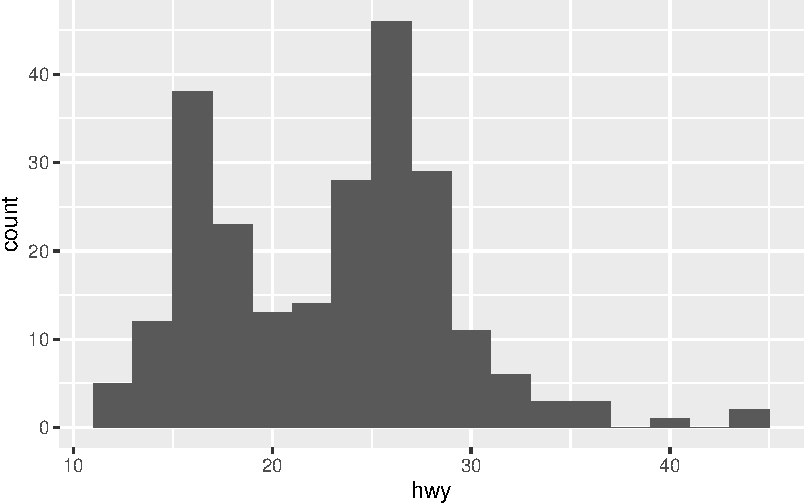
\includegraphics{Fatores/Fatores_com_forcats_files/figure-pdf/unnamed-chunk-37-1.pdf}

}

\end{figure}

Veja que neste exemplo, pedimos para a funções fct\_lump\_n agrupar tudo
em um grupo, exceto os 3 maiores grupos. Veja que tivemos 4 grupo + 1
``other'' pois ouve um empate no terceiro grupo. Depois, como queríamos
que o grupo ``other'' ficava abaixo do gráfico, optamos por deslocar em
-1 inteiro a nível deste fator, fazendo com o primeiro nível fosse para
o último lugar.

\hypertarget{fct_other}{%
\subsubsection{fct\_other}\label{fct_other}}

Use para definir \textbf{manualmente} os níveis que irão pertecer ao
grupo ``other''.

\begin{Shaded}
\begin{Highlighting}[]
\NormalTok{f}
\end{Highlighting}
\end{Shaded}

\begin{verbatim}
[1] a c b a
Levels: a b c
\end{verbatim}

\begin{Shaded}
\begin{Highlighting}[]
\FunctionTok{fct\_other}\NormalTok{(f, }\AttributeTok{keep =} \FunctionTok{c}\NormalTok{(}\StringTok{"a"}\NormalTok{, }\StringTok{"b"}\NormalTok{))}
\end{Highlighting}
\end{Shaded}

\begin{verbatim}
[1] a     Other b     a    
Levels: a b Other
\end{verbatim}

\hypertarget{adicionando-ou-removendo-nuxedveis}{%
\section{Adicionando ou Removendo
Níveis}\label{adicionando-ou-removendo-nuxedveis}}

\hypertarget{fct_drop}{%
\subsubsection{fct\_drop}\label{fct_drop}}

Use para remover níveis que não estão sendo usados.

\begin{Shaded}
\begin{Highlighting}[]
\NormalTok{f5 }\OtherTok{\textless{}{-}} \FunctionTok{factor}\NormalTok{(}\FunctionTok{c}\NormalTok{(}\StringTok{"a"}\NormalTok{,}\StringTok{"b"}\NormalTok{),}\FunctionTok{c}\NormalTok{(}\StringTok{"a"}\NormalTok{,}\StringTok{"b"}\NormalTok{,}\StringTok{"x"}\NormalTok{))}
\NormalTok{f5}
\end{Highlighting}
\end{Shaded}

\begin{verbatim}
[1] a b
Levels: a b x
\end{verbatim}

\begin{Shaded}
\begin{Highlighting}[]
\NormalTok{f6 }\OtherTok{\textless{}{-}} \FunctionTok{fct\_drop}\NormalTok{(f5)}
\NormalTok{f6}
\end{Highlighting}
\end{Shaded}

\begin{verbatim}
[1] a b
Levels: a b
\end{verbatim}

\hypertarget{fct_expand}{%
\subsubsection{fct\_expand}\label{fct_expand}}

Use para adicionar níveis a um fator.

\begin{Shaded}
\begin{Highlighting}[]
\FunctionTok{fct\_expand}\NormalTok{(f6, }\StringTok{"x"}\NormalTok{)}
\end{Highlighting}
\end{Shaded}

\begin{verbatim}
[1] a b
Levels: a b x
\end{verbatim}

\hypertarget{fct_explicit_na}{%
\subsubsection{fct\_explicit\_na}\label{fct_explicit_na}}

Use para definir níveis ``NA'' como (Missing). Isto é útil quando quiser
deixar explícito em gráficos os valores ausentes (Missings).

\begin{Shaded}
\begin{Highlighting}[]
\FunctionTok{fct\_explicit\_na}\NormalTok{(}\FunctionTok{factor}\NormalTok{(}\FunctionTok{c}\NormalTok{(}\StringTok{"a"}\NormalTok{, }\StringTok{"b"}\NormalTok{, }\ConstantTok{NA}\NormalTok{)))}
\end{Highlighting}
\end{Shaded}

\begin{verbatim}
[1] a         b         (Missing)
Levels: a b (Missing)
\end{verbatim}

\begin{Shaded}
\begin{Highlighting}[]
\NormalTok{tb }\OtherTok{\textless{}{-}} \FunctionTok{tribble}\NormalTok{(}\SpecialCharTok{\textasciitilde{}}\NormalTok{x, }\SpecialCharTok{\textasciitilde{}}\NormalTok{y,}
        \StringTok{"A"}\NormalTok{, }\DecValTok{1}\NormalTok{,}
        \StringTok{"A"}\NormalTok{, }\DecValTok{2}\NormalTok{,}
        \StringTok{"A"}\NormalTok{, }\DecValTok{2}\NormalTok{,}
        \StringTok{"B"}\NormalTok{, }\DecValTok{3}\NormalTok{,}
        \ConstantTok{NA}\NormalTok{, }\ConstantTok{NA}\NormalTok{,}
        \StringTok{"D"}\NormalTok{, }\DecValTok{5}\NormalTok{,}
        \ConstantTok{NA}\NormalTok{, }\ConstantTok{NA}\NormalTok{,}
        \StringTok{"D"}\NormalTok{, }\DecValTok{4}\NormalTok{,)}

\NormalTok{tb}\SpecialCharTok{$}\NormalTok{x }\OtherTok{\textless{}{-}} \FunctionTok{as\_factor}\NormalTok{(tb}\SpecialCharTok{$}\NormalTok{x)}

\NormalTok{tb }\SpecialCharTok{|\textgreater{}} \FunctionTok{ggplot}\NormalTok{(}\FunctionTok{aes}\NormalTok{(x)) }\SpecialCharTok{+}
  \FunctionTok{geom\_bar}\NormalTok{()}
\NormalTok{tb }\SpecialCharTok{|\textgreater{}} \FunctionTok{ggplot}\NormalTok{(}\FunctionTok{aes}\NormalTok{(}\FunctionTok{fct\_explicit\_na}\NormalTok{(x, }\AttributeTok{na\_level =} \StringTok{"Sem Valores"}\NormalTok{))) }\SpecialCharTok{+}
  \FunctionTok{geom\_bar}\NormalTok{()}
\end{Highlighting}
\end{Shaded}

\begin{figure}

\begin{minipage}[t]{0.50\linewidth}

{\centering 

\raisebox{-\height}{

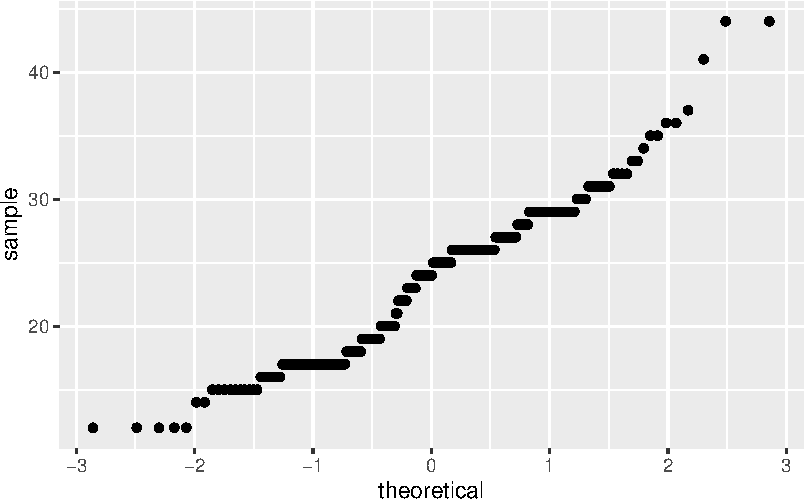
\includegraphics{Fatores/Fatores_com_forcats_files/figure-pdf/unnamed-chunk-42-1.pdf}

}

}

\end{minipage}%
%
\begin{minipage}[t]{0.50\linewidth}

{\centering 

\raisebox{-\height}{

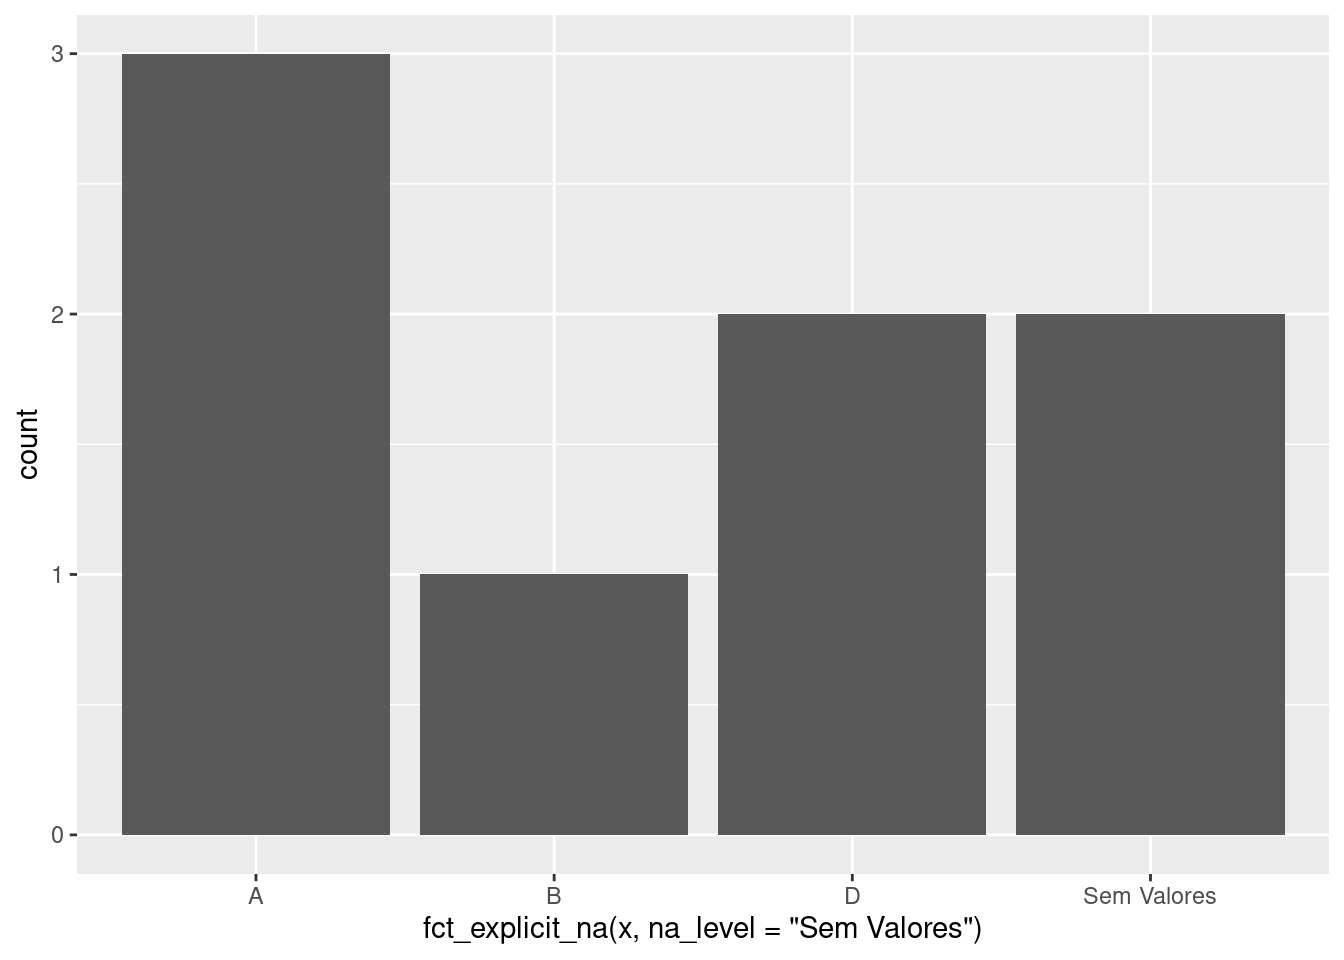
\includegraphics{Fatores/Fatores_com_forcats_files/figure-pdf/unnamed-chunk-42-2.pdf}

}

}

\end{minipage}%

\end{figure}

\part{Parte 3 - Trabalhando com Data e Programação Funcional}

\hypertarget{datas-e-horas-com-lubridate}{%
\chapter{Datas e horas com
LUBRIDATE}\label{datas-e-horas-com-lubridate}}

\hypertarget{introduuxe7uxe3o-8}{%
\section{Introdução}\label{introduuxe7uxe3o-8}}

A seguir temos vários exemplos de manipulação de \textbf{variáveis}
\textbf{data e hora} utilizando o pacote LUBRIDATE do R. Para saber mais
sobre este pacote, acesse:

\url{https://cran.r-project.org/package=lubridate}.

\begin{tcolorbox}[enhanced jigsaw, rightrule=.15mm, arc=.35mm, coltitle=black, colframe=quarto-callout-warning-color-frame, opacityback=0, toprule=.15mm, left=2mm, breakable, colback=white, bottomtitle=1mm, leftrule=.75mm, title=\textcolor{quarto-callout-warning-color}{\faExclamationTriangle}\hspace{0.5em}{Aviso}, colbacktitle=quarto-callout-warning-color!10!white, titlerule=0mm, bottomrule=.15mm, toptitle=1mm, opacitybacktitle=0.6]
Para melhor utilizar este material, é importante que você tenha uma
introdução à linguagem R e saiba carregar pacotes (packages) no R. Para
mais informações acesse:

\url{https://education.rstudio.com/learn/beginner/}.
\end{tcolorbox}

Para os exemplos, iremos carregar os seguintes pacotes:

\begin{itemize}
\item
  \textbf{tidyverse}
\item
  \textbf{gt}
\item
  \textbf{lubridate}
\end{itemize}

\begin{Shaded}
\begin{Highlighting}[]
\FunctionTok{library}\NormalTok{ (tidyverse)}
\FunctionTok{library}\NormalTok{ (gt)}
\FunctionTok{library}\NormalTok{ (lubridate)}
\end{Highlighting}
\end{Shaded}

\hypertarget{tipos-de-objetos-de-data-e-hora}{%
\section{Tipos de objetos de data e
hora}\label{tipos-de-objetos-de-data-e-hora}}

\hypertarget{datetime}{%
\subsubsection{Datetime}\label{datetime}}

Uma variável do tipo ``\textbf{datetime}'' (\emph{data e hora})
representa um ponto na linha do tempo armazenado em um número que
representa o número de \textbf{segundos} desde \textbf{01-01-1970
00:00:00 (UTC)}.

\begin{tcolorbox}[enhanced jigsaw, rightrule=.15mm, arc=.35mm, coltitle=black, colframe=quarto-callout-note-color-frame, opacityback=0, toprule=.15mm, left=2mm, breakable, colback=white, bottomtitle=1mm, leftrule=.75mm, title=\textcolor{quarto-callout-note-color}{\faInfo}\hspace{0.5em}{Nota}, colbacktitle=quarto-callout-note-color!10!white, titlerule=0mm, bottomrule=.15mm, toptitle=1mm, opacitybacktitle=0.6]
Universal Time Coordinated (\textbf{UTC}), é uma escala coordenada de
tempo, mantida pelo ``Bureau International des Poids et Mesures
(BIPM)''. Até 1972, era chamado de (\textbf{GTM} ou \emph{Greenwich Mean
Time}). É também conhecida como ``Z time'' ou ``Zulu Time''.
\end{tcolorbox}

\hypertarget{date}{%
\subsubsection{Date}\label{date}}

Quando nos referimos à uma variável ``\textbf{date}''(\emph{data}),
significa que ela armazena um número inteiro que representa o número de
\textbf{dias} \textbf{desde 01-01-1970.}

\hypertarget{time}{%
\subsubsection{\texorpdfstring{\textbf{Time}}{Time}}\label{time}}

Quando nos referimos à uma variável ``\textbf{time}'' (tempo em
segundos), ela armazena um número inteiro que representa o número de
\textbf{segundos} \textbf{desde às} \textbf{00:00:00} (hms).

Para os vários exemplos a seguir, utilizaremos os seguintes objetos data
e hora:

\begin{Shaded}
\begin{Highlighting}[]
\NormalTok{dt }\OtherTok{\textless{}{-}}  \FunctionTok{as\_datetime}\NormalTok{(}\DecValTok{1511870400}\NormalTok{)}
\NormalTok{d }\OtherTok{\textless{}{-}} \FunctionTok{as\_date}\NormalTok{(}\DecValTok{17498}\NormalTok{)}
\NormalTok{t }\OtherTok{\textless{}{-}}\NormalTok{hms}\SpecialCharTok{::}\FunctionTok{as\_hms}\NormalTok{(}\DecValTok{85}\NormalTok{)}
\NormalTok{dt; d; t}
\end{Highlighting}
\end{Shaded}

\begin{verbatim}
[1] "2017-11-28 12:00:00 UTC"
\end{verbatim}

\begin{verbatim}
[1] "2017-11-28"
\end{verbatim}

\begin{verbatim}
00:01:25
\end{verbatim}

\begin{tcolorbox}[enhanced jigsaw, rightrule=.15mm, arc=.35mm, coltitle=black, colframe=quarto-callout-tip-color-frame, opacityback=0, toprule=.15mm, left=2mm, breakable, colback=white, bottomtitle=1mm, leftrule=.75mm, title=\textcolor{quarto-callout-tip-color}{\faLightbulb}\hspace{0.5em}{Dica}, colbacktitle=quarto-callout-tip-color!10!white, titlerule=0mm, bottomrule=.15mm, toptitle=1mm, opacitybacktitle=0.6]
Os objetos gerados pela maioria das funções do lubridate usam os padrões
POSIXct, POSIXlt, Date, Period ou objetos que podem ser convertidos para
o POSIXlt. Para maiores informações sobre estas classes, digite:

?DateTimeClasses

POSIXct: armazena segundos desde 01-01-1970 00:00:00 (Unix epoch)
POSIXlt: armazena uma lista de dia, mês, ano, hora, min, segundos, etc.
\end{tcolorbox}

\hypertarget{exemplos-da-folha-de-referuxeancia-5}{%
\subsection{Exemplos da Folha de
Referência}\label{exemplos-da-folha-de-referuxeancia-5}}

A maioria dos exemplos, visam ajudar na interpretação dos exemplos e
funções encontradas na
\href{https://github.com/scopinho/R-cheatsheets/blob/main/translations/portuguese/lubridate_pt_br.pdf}{\textbf{Folha
de Referência}} do lubridate disponível no site do
\href{rstudio.com}{RStudio}.

\begin{figure}

{\centering 

\href{images/cs-lubridate-01.png}{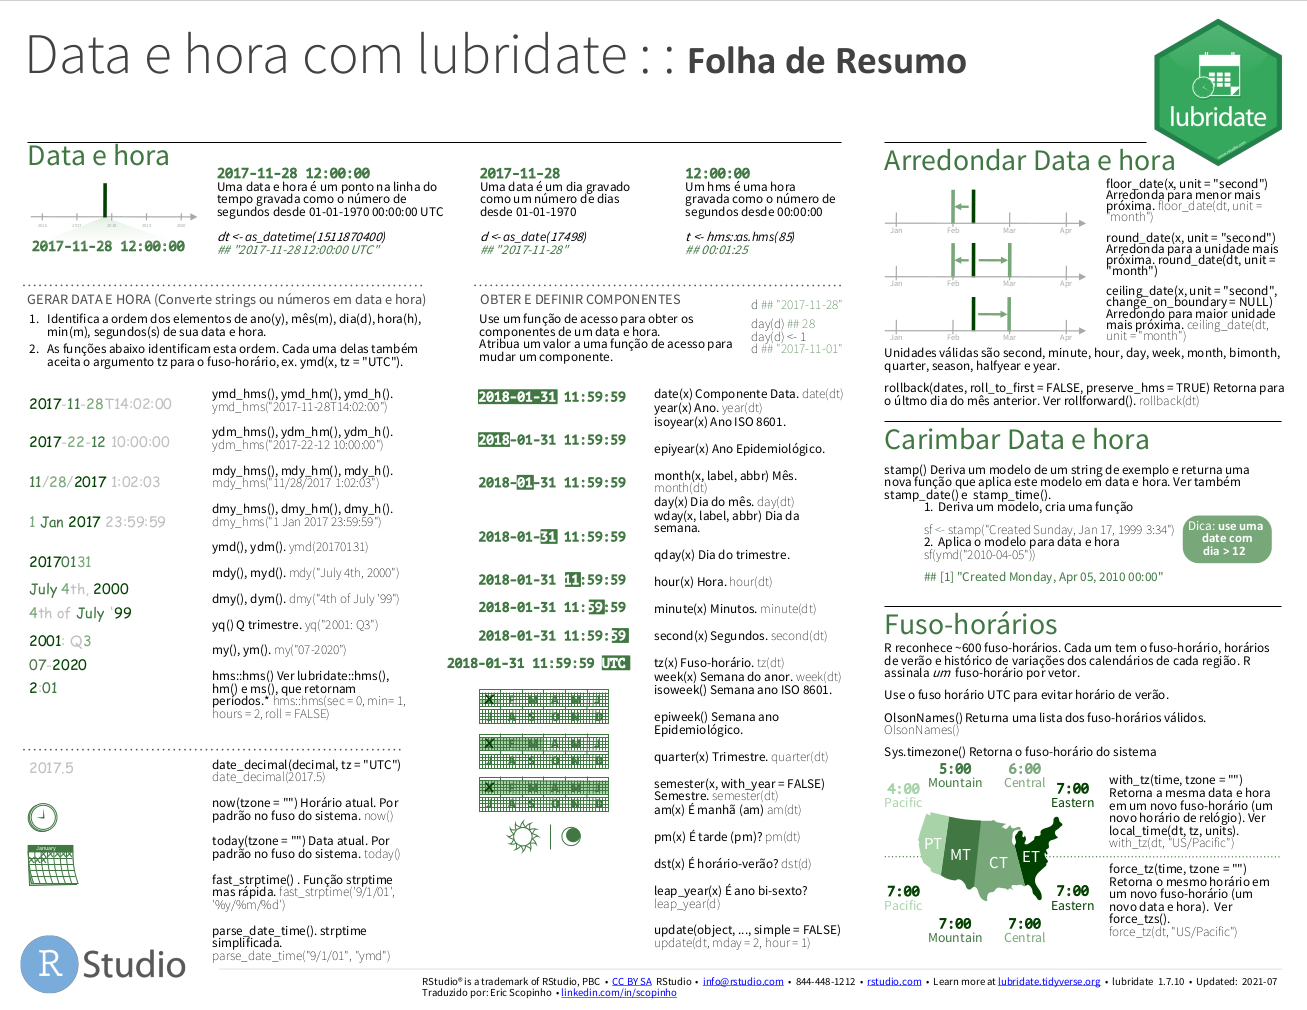
\includegraphics{DataHora/images/cs-lubridate-01.png}}

}

\end{figure}

\begin{figure}

{\centering 

\href{images/cs-lubridate-02.png}{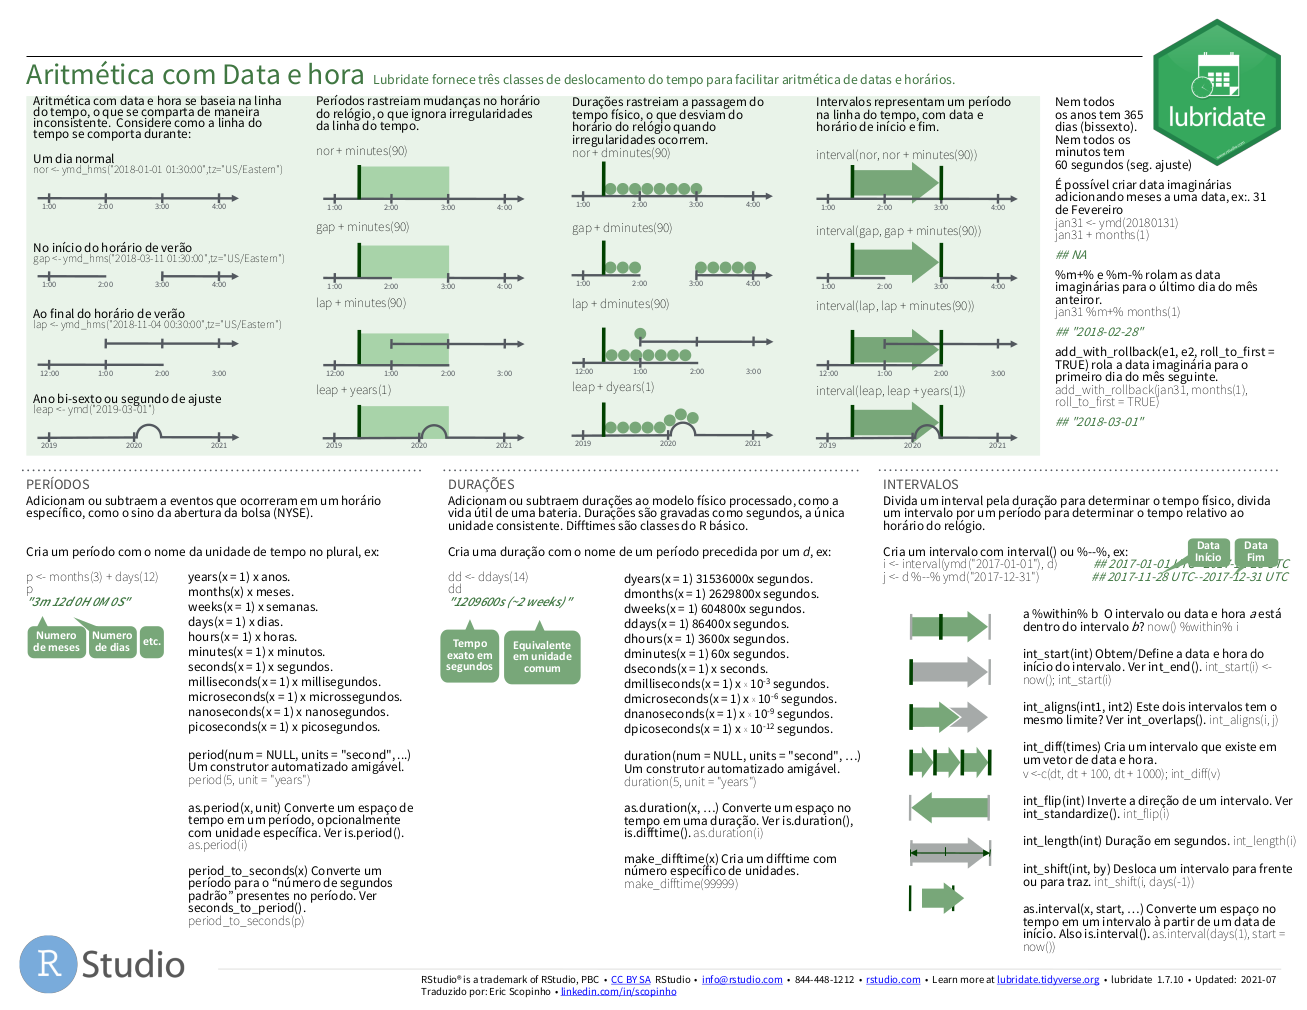
\includegraphics{DataHora/images/cs-lubridate-02.png}}

}

\end{figure}

\begin{center}\rule{0.5\linewidth}{0.5pt}\end{center}

\begin{tcolorbox}[enhanced jigsaw, rightrule=.15mm, arc=.35mm, coltitle=black, colframe=quarto-callout-note-color-frame, opacityback=0, toprule=.15mm, left=2mm, breakable, colback=white, bottomtitle=1mm, leftrule=.75mm, title=\textcolor{quarto-callout-note-color}{\faInfo}\hspace{0.5em}{Nota}, colbacktitle=quarto-callout-note-color!10!white, titlerule=0mm, bottomrule=.15mm, toptitle=1mm, opacitybacktitle=0.6]
\emph{Em geral, ao final de cada comando, as vezes você verá a chamada à
função \textbf{gt()}. Isto é apenas para a formatação da tabela de saída
e não é necessário para que você entenda os comandos precedentes. Em
alguns casos, onde o volume de dados de saída pode ser extenso, usamos
também a função \textbf{head()} para mostrar apenas as linhas iniciais.
Quando o exemplo possui muitas colunas de saída, eventualmente
utilizamos a função \textbf{select()} para selecionar apenas algumas
colunas.}

Em alguns casos usaremos funções de manipulação de dados do pacote
\textbf{dplyr,} como \textbf{mutate} () ou \textbf{count}()\textbf{.}
\end{tcolorbox}

\begin{tcolorbox}[enhanced jigsaw, rightrule=.15mm, arc=.35mm, coltitle=black, colframe=quarto-callout-note-color-frame, opacityback=0, toprule=.15mm, left=2mm, breakable, colback=white, bottomtitle=1mm, leftrule=.75mm, title=\textcolor{quarto-callout-note-color}{\faInfo}\hspace{0.5em}{Nota}, colbacktitle=quarto-callout-note-color!10!white, titlerule=0mm, bottomrule=.15mm, toptitle=1mm, opacitybacktitle=0.6]
\emph{O termo \uline{data-frame} descrito ao longo deste texto, é
utilizado de forma livre para objetos do tipo data.frame, tibble, entre
outros. Pense como se fosse uma tabela de um banco de dados e/ou uma
planilha do MS Excel, contendo linhas e colunas. Apesar de não ser
rigorosamente igual à uma tabela, muitas vezes usaremos estes termos de
forma intercambiável para facilitar o entendimento de iniciantes.}
\end{tcolorbox}

\hypertarget{validando-data-e-hora}{%
\section{Validando Data e Hora}\label{validando-data-e-hora}}

O pacote lubridate possui uma série de funções para obter e definir os
elementos de ano, mês, dia, hora, minuto e segundos de um objeto data e
hora.

Use as funções a seguir servem para identificar estes elementos em seus
dados a partir de uma string. Cada uma delas aceita o argumento ``tz''
para definir o fuso-horário (\emph{timezone}), se este não for definido,
UTC é utilizado.

Estas funções são nomeadas conforme a tabela abaixo e sua ordem obedece
tal nomenclatura:

\begin{longtable}[]{@{}ll@{}}
\toprule()
Elemento & Letra \\
\midrule()
\endhead
y & ano (\emph{year}) \\
m & mês (\emph{month}) \\
d & dia (\emph{day}) \\
h & hora (\emph{hour}) \\
m & minuto (\emph{minute}) \\
s & segundos (\emph{seconds}) \\
\bottomrule()
\end{longtable}

Por exemplo, para criar um objeto \textbf{datetime} passando a string
``\textbf{2017-11-28T14:02:00}'', utilzamos a função
\textbf{ymd\_hms}(). Isto porque ao montar a string de data e hora,
colocamos como ordem o ano, mês, dia, hora, minuto e segundo.

\begin{Shaded}
\begin{Highlighting}[]
\FunctionTok{ymd\_hms}\NormalTok{(}\StringTok{"2017{-}11{-}28T14:02:00"}\NormalTok{)}
\end{Highlighting}
\end{Shaded}

\begin{verbatim}
[1] "2017-11-28 14:02:00 UTC"
\end{verbatim}

Se passarmos a string trocando o ano pela dia, devemos usar a função
dmy\_hms():

\begin{Shaded}
\begin{Highlighting}[]
\FunctionTok{dmy\_hms}\NormalTok{(}\StringTok{"28{-}11{-}2017T14:02:00"}\NormalTok{)}
\end{Highlighting}
\end{Shaded}

\begin{verbatim}
[1] "2017-11-28 14:02:00 UTC"
\end{verbatim}

\begin{tcolorbox}[enhanced jigsaw, rightrule=.15mm, arc=.35mm, coltitle=black, colframe=quarto-callout-note-color-frame, opacityback=0, toprule=.15mm, left=2mm, breakable, colback=white, bottomtitle=1mm, leftrule=.75mm, title=\textcolor{quarto-callout-note-color}{\faInfo}\hspace{0.5em}{Nota}, colbacktitle=quarto-callout-note-color!10!white, titlerule=0mm, bottomrule=.15mm, toptitle=1mm, opacitybacktitle=0.6]
Veja que tanto a função ymd\_hms() quanto a dmy\_hms(), geraram o mesmo
objeto datetime. Se quisermos obter o valor inteiro que representa este
objeto desde 01-01-1970 00:00:00, podemos usar a função
\textbf{decimal\_date}()
\end{tcolorbox}

Veja o código abaixo com mais alguns exemplos das funções validando os
elementos da string passada para a função:

\begin{Shaded}
\begin{Highlighting}[]
\CommentTok{\# ymd\_hms(), ymd\_hm(), ymd\_h().}
\FunctionTok{ymd\_hms}\NormalTok{(}\StringTok{"2017{-}11{-}28T14:02:00"}\NormalTok{) }\SpecialCharTok{|\textgreater{}} \FunctionTok{print}\NormalTok{()}
\end{Highlighting}
\end{Shaded}

\begin{verbatim}
[1] "2017-11-28 14:02:00 UTC"
\end{verbatim}

\begin{Shaded}
\begin{Highlighting}[]
\CommentTok{\# ydm\_hms(), ydm\_hm(), ydm\_h().}
\FunctionTok{ydm\_hms}\NormalTok{(}\StringTok{"2017{-}22{-}12 10:00:00"}\NormalTok{) }\SpecialCharTok{|\textgreater{}}  \FunctionTok{print}\NormalTok{()}
\end{Highlighting}
\end{Shaded}

\begin{verbatim}
[1] "2017-12-22 10:00:00 UTC"
\end{verbatim}

\begin{Shaded}
\begin{Highlighting}[]
\CommentTok{\# mdy\_hms(), mdy\_hm(), mdy\_h(). }
\FunctionTok{mdy\_hms}\NormalTok{(}\StringTok{"11/28/2017 1:02:03"}\NormalTok{) }\SpecialCharTok{|\textgreater{}}  \FunctionTok{print}\NormalTok{()}
\end{Highlighting}
\end{Shaded}

\begin{verbatim}
[1] "2017-11-28 01:02:03 UTC"
\end{verbatim}

\begin{Shaded}
\begin{Highlighting}[]
\CommentTok{\# dmy\_hms(), dmy\_hm(), dmy\_h().}
\FunctionTok{dmy\_hms}\NormalTok{(}\StringTok{"1 Jan 2017 23:59:59"}\NormalTok{)}\SpecialCharTok{|\textgreater{}}  \FunctionTok{print}\NormalTok{()}
\end{Highlighting}
\end{Shaded}

\begin{verbatim}
[1] "2017-01-01 23:59:59 UTC"
\end{verbatim}

\begin{Shaded}
\begin{Highlighting}[]
\CommentTok{\# ymd(), ydm(). }
\FunctionTok{ymd}\NormalTok{(}\DecValTok{20170131}\NormalTok{)}\SpecialCharTok{|\textgreater{}}  \FunctionTok{print}\NormalTok{()}
\end{Highlighting}
\end{Shaded}

\begin{verbatim}
[1] "2017-01-31"
\end{verbatim}

\begin{Shaded}
\begin{Highlighting}[]
\CommentTok{\# mdy(), myd(). }
\FunctionTok{mdy}\NormalTok{(}\StringTok{"July 4th, 2000"}\NormalTok{)}\SpecialCharTok{|\textgreater{}}  \FunctionTok{print}\NormalTok{()}
\end{Highlighting}
\end{Shaded}

\begin{verbatim}
[1] "2000-07-04"
\end{verbatim}

\begin{Shaded}
\begin{Highlighting}[]
\CommentTok{\# dmy(), dym(). }
\FunctionTok{dmy}\NormalTok{(}\StringTok{"4th of July \textquotesingle{}99"}\NormalTok{)}\SpecialCharTok{|\textgreater{}}  \FunctionTok{print}\NormalTok{()}
\end{Highlighting}
\end{Shaded}

\begin{verbatim}
[1] "1999-07-04"
\end{verbatim}

\begin{Shaded}
\begin{Highlighting}[]
\CommentTok{\# yq() Q para quartil. }
\FunctionTok{yq}\NormalTok{(}\StringTok{"2001: Q3"}\NormalTok{)}\SpecialCharTok{|\textgreater{}}  \FunctionTok{print}\NormalTok{()}
\end{Highlighting}
\end{Shaded}

\begin{verbatim}
[1] "2001-07-01"
\end{verbatim}

\begin{Shaded}
\begin{Highlighting}[]
\CommentTok{\# my(), ym(). }
\FunctionTok{my}\NormalTok{(}\StringTok{"07{-}2020"}\NormalTok{)}\SpecialCharTok{|\textgreater{}}  \FunctionTok{print}\NormalTok{()}
\end{Highlighting}
\end{Shaded}

\begin{verbatim}
[1] "2020-07-01"
\end{verbatim}

\begin{Shaded}
\begin{Highlighting}[]
\CommentTok{\#hms::hms() ou lubridate::hms(), ms() ou hm() para períodos.}
\NormalTok{hms}\SpecialCharTok{::}\FunctionTok{hms}\NormalTok{(}\AttributeTok{sec =} \DecValTok{0}\NormalTok{, }\AttributeTok{min =} \DecValTok{1}\NormalTok{, }\AttributeTok{hours =} \DecValTok{2}\NormalTok{)}
\end{Highlighting}
\end{Shaded}

\begin{verbatim}
02:01:00
\end{verbatim}

\hypertarget{outras-funuxe7uxf5es-uxfateis}{%
\subsection{Outras funções úteis}\label{outras-funuxe7uxf5es-uxfateis}}

\hypertarget{date_decimal}{%
\subsubsection{date\_decimal}\label{date_decimal}}

Use para converter um número decimala para data e hora:

\begin{Shaded}
\begin{Highlighting}[]
\FunctionTok{date\_decimal}\NormalTok{(}\FloatTok{2017.5}\NormalTok{)}
\end{Highlighting}
\end{Shaded}

\begin{verbatim}
[1] "2017-07-02 12:00:00 UTC"
\end{verbatim}

\hypertarget{now}{%
\subsubsection{now}\label{now}}

Use para obter um objeto data e hora do instante:

\begin{Shaded}
\begin{Highlighting}[]
\FunctionTok{now}\NormalTok{(}\AttributeTok{tzone =} \StringTok{"America/Sao\_Paulo"}\NormalTok{)}
\end{Highlighting}
\end{Shaded}

\begin{verbatim}
[1] "2022-09-12 11:19:17 -03"
\end{verbatim}

\begin{tcolorbox}[enhanced jigsaw, rightrule=.15mm, arc=.35mm, coltitle=black, colframe=quarto-callout-important-color-frame, opacityback=0, toprule=.15mm, left=2mm, breakable, colback=white, bottomtitle=1mm, leftrule=.75mm, title=\textcolor{quarto-callout-important-color}{\faExclamation}\hspace{0.5em}{Importante}, colbacktitle=quarto-callout-important-color!10!white, titlerule=0mm, bottomrule=.15mm, toptitle=1mm, opacitybacktitle=0.6]
Se o fuso-horário (tzone =) não for informado, a função utilizará aquele
utilzado pelo sitema operacional em execução.
\end{tcolorbox}

\hypertarget{today}{%
\subsubsection{today}\label{today}}

Use para obter a data atual.

\begin{Shaded}
\begin{Highlighting}[]
\FunctionTok{today}\NormalTok{()}
\end{Highlighting}
\end{Shaded}

\begin{verbatim}
[1] "2022-09-12"
\end{verbatim}

\hypertarget{fast_strptime}{%
\subsubsection{fast\_strptime}\label{fast_strptime}}

Use para converter vetores de caracteres para objetos data e hora
(POSIXlt) de forma rápida.

\begin{Shaded}
\begin{Highlighting}[]
\FunctionTok{fast\_strptime}\NormalTok{(}\StringTok{\textquotesingle{}9/1/01\textquotesingle{}}\NormalTok{, }\StringTok{\textquotesingle{}\%y/\%m/\%d\textquotesingle{}}\NormalTok{)}
\end{Highlighting}
\end{Shaded}

\begin{verbatim}
[1] "2009-01-01 UTC"
\end{verbatim}

\hypertarget{parse_date_time}{%
\subsubsection{parse\_date\_time}\label{parse_date_time}}

Use para converter vetores de caracteres para objetos data e hora
(POSIXct) de forma mais simplificada.

\begin{Shaded}
\begin{Highlighting}[]
\FunctionTok{parse\_date\_time}\NormalTok{(}\StringTok{"19/1/1"}\NormalTok{, }\StringTok{"ymd"}\NormalTok{)}
\end{Highlighting}
\end{Shaded}

\begin{verbatim}
[1] "2019-01-01 UTC"
\end{verbatim}

\hypertarget{obtendo-e-definindo-componentes-de-data-e-hora}{%
\section{Obtendo e Definindo Componentes de Data e
Hora}\label{obtendo-e-definindo-componentes-de-data-e-hora}}

Use as funções abaixo para obter um componente de um objeto data e hora.

\begin{Shaded}
\begin{Highlighting}[]
\CommentTok{\# Obter o "DIA" de um objeto "datetime"}
\FunctionTok{day}\NormalTok{(dt)}
\end{Highlighting}
\end{Shaded}

\begin{verbatim}
[1] 28
\end{verbatim}

\begin{Shaded}
\begin{Highlighting}[]
\CommentTok{\# Obter a "DATA"}
\FunctionTok{date}\NormalTok{(dt)}
\end{Highlighting}
\end{Shaded}

\begin{verbatim}
[1] "2017-11-28"
\end{verbatim}

\begin{Shaded}
\begin{Highlighting}[]
\CommentTok{\# Obter a "ANO".}
\CommentTok{\# Para obter o "ANO ISO 8610 use isoyear()}
\CommentTok{\# Para obter o "ANO Epidemiológico use epiyear()}
\FunctionTok{year}\NormalTok{(dt)}
\end{Highlighting}
\end{Shaded}

\begin{verbatim}
[1] 2017
\end{verbatim}

\begin{Shaded}
\begin{Highlighting}[]
\CommentTok{\# Obter o "MÊS". }
\CommentTok{\# Use argumentos label= e addr= para obter o nome ou abreviação do mês.}
\FunctionTok{month}\NormalTok{(dt)}
\end{Highlighting}
\end{Shaded}

\begin{verbatim}
[1] 11
\end{verbatim}

\begin{Shaded}
\begin{Highlighting}[]
\CommentTok{\# Obter o "DIA DA SEMANA".}
\CommentTok{\# Use argumentos label= e addr= para obter o nome ou abreviação do dia.}
\FunctionTok{wday}\NormalTok{(dt, }\AttributeTok{label =} \ConstantTok{TRUE}\NormalTok{) }
\end{Highlighting}
\end{Shaded}

\begin{verbatim}
[1] ter
Levels: dom < seg < ter < qua < qui < sex < sáb
\end{verbatim}

\begin{Shaded}
\begin{Highlighting}[]
\CommentTok{\# Obter o "DIA DO TRIMESTRE".}
\FunctionTok{qday}\NormalTok{(dt) }
\end{Highlighting}
\end{Shaded}

\begin{verbatim}
[1] 59
\end{verbatim}

\begin{Shaded}
\begin{Highlighting}[]
\CommentTok{\# Obter a HORA". }
\FunctionTok{hour}\NormalTok{(dt)}
\end{Highlighting}
\end{Shaded}

\begin{verbatim}
[1] 12
\end{verbatim}

\begin{Shaded}
\begin{Highlighting}[]
\CommentTok{\# Obter os "MINUTOS". }
\FunctionTok{minute}\NormalTok{(dt)}
\end{Highlighting}
\end{Shaded}

\begin{verbatim}
[1] 0
\end{verbatim}

\begin{Shaded}
\begin{Highlighting}[]
\CommentTok{\# Obter os "SEGUNDOS". }
\FunctionTok{second}\NormalTok{(dt)}
\end{Highlighting}
\end{Shaded}

\begin{verbatim}
[1] 0
\end{verbatim}

\begin{Shaded}
\begin{Highlighting}[]
\CommentTok{\# Obter o "FUSO{-}HORÁRIO. }
\FunctionTok{tz}\NormalTok{(dt)}
\end{Highlighting}
\end{Shaded}

\begin{verbatim}
[1] "UTC"
\end{verbatim}

\begin{Shaded}
\begin{Highlighting}[]
\CommentTok{\# Obter a "SEMANA DO ANO". }
\FunctionTok{week}\NormalTok{(dt)}
\end{Highlighting}
\end{Shaded}

\begin{verbatim}
[1] 48
\end{verbatim}

\begin{Shaded}
\begin{Highlighting}[]
\CommentTok{\# ara obter a "SEMANA DO ANO" ISO 8160 use isoyear()}
\CommentTok{\# Para obter a "SEMANA DO ANO" Epidemiológico use epiyear()}

\CommentTok{\# Obter o "TRIMESTRE". }
\FunctionTok{quarter}\NormalTok{(dt)}
\end{Highlighting}
\end{Shaded}

\begin{verbatim}
[1] 4
\end{verbatim}

\begin{Shaded}
\begin{Highlighting}[]
\CommentTok{\# Obter o "SEMESTRE". }
\FunctionTok{semester}\NormalTok{(dt)}
\end{Highlighting}
\end{Shaded}

\begin{verbatim}
[1] 2
\end{verbatim}

\begin{Shaded}
\begin{Highlighting}[]
\CommentTok{\# Saber se é "MANHÃ (am). }
\FunctionTok{am}\NormalTok{(dt)}
\end{Highlighting}
\end{Shaded}

\begin{verbatim}
[1] FALSE
\end{verbatim}

\begin{Shaded}
\begin{Highlighting}[]
\CommentTok{\# Saber se é "TARDE" (pm).}
\FunctionTok{pm}\NormalTok{(dt)}
\end{Highlighting}
\end{Shaded}

\begin{verbatim}
[1] TRUE
\end{verbatim}

\begin{Shaded}
\begin{Highlighting}[]
\CommentTok{\# Saber se é "HORÁRIO DE VERÃO" }
\FunctionTok{dst}\NormalTok{(d)}
\end{Highlighting}
\end{Shaded}

\begin{verbatim}
[1] FALSE
\end{verbatim}

\begin{Shaded}
\begin{Highlighting}[]
\CommentTok{\# Saber se é "ANO BISEXTO"}
\FunctionTok{leap\_year}\NormalTok{(d)}
\end{Highlighting}
\end{Shaded}

\begin{verbatim}
[1] FALSE
\end{verbatim}

Para definir um componente de um objeto, podemos utilzar as funções
acima, porém com o sinal de atribuição.

Por exemplo, para alterar o dia de ``28'' do objeto ``d'', para dia
``1'', podemos fazer:

\begin{Shaded}
\begin{Highlighting}[]
\FunctionTok{day}\NormalTok{(d) }\SpecialCharTok{|\textgreater{}}  \FunctionTok{print}\NormalTok{() }
\end{Highlighting}
\end{Shaded}

\begin{verbatim}
[1] 28
\end{verbatim}

\begin{Shaded}
\begin{Highlighting}[]
\FunctionTok{day}\NormalTok{(d) }\OtherTok{\textless{}{-}} \DecValTok{1}
\FunctionTok{print}\NormalTok{(d) }
\end{Highlighting}
\end{Shaded}

\begin{verbatim}
[1] "2017-11-01"
\end{verbatim}

Podemos também atualizar um componente do objeto data e hora:

\begin{Shaded}
\begin{Highlighting}[]
\CommentTok{\# Atualizar um componente do objeto}
\FunctionTok{update}\NormalTok{(dt, }\AttributeTok{mday =} \DecValTok{2}\NormalTok{, }\AttributeTok{hour =} \DecValTok{1}\NormalTok{)}
\end{Highlighting}
\end{Shaded}

\begin{verbatim}
[1] "2017-11-02 01:00:00 UTC"
\end{verbatim}

O exemplo acima, altera o dia do mês para 2 e a hora para 01.

\hypertarget{arredondando-data-e-hora}{%
\section{Arredondando Data e Hora}\label{arredondando-data-e-hora}}

Use as funções a seguir para ``arredondar'' ou aproximar um objeto data
e hora para unidades de ajuste. As unidades válidas são:

\begin{itemize}
\tightlist
\item
  \emph{second, minute, hour, day, week, month, bimonth, quarter,
  season, halfyear e year.}
\end{itemize}

\hypertarget{floor_date}{%
\subsubsection{floor\_date}\label{floor_date}}

Use para ``\textbf{arredondar para baixo}'' a data e hora para a unidade
mais próxima.

Por exemplo, digamos que temos um objeto data = ``2017-11-28'' e
queremos arredondar para baixo, sendo que a unidade é mês, ou seja,
arredondar para o início do mês:

\begin{Shaded}
\begin{Highlighting}[]
\FunctionTok{floor\_date}\NormalTok{(dt, }\AttributeTok{unit=}\StringTok{"month"}\NormalTok{)}
\end{Highlighting}
\end{Shaded}

\begin{verbatim}
[1] "2017-11-01 UTC"
\end{verbatim}

round\_date

Use para ``\textbf{arredondar}'' a data para a unidade mais próxima.

\begin{Shaded}
\begin{Highlighting}[]
\FunctionTok{round\_date}\NormalTok{(dt, }\AttributeTok{unit=}\StringTok{"month"}\NormalTok{)}
\end{Highlighting}
\end{Shaded}

\begin{verbatim}
[1] "2017-12-01 UTC"
\end{verbatim}

Veja que no exemplo acima, como tínhamos dia 28/11 e pedimos para
arredondar na unidade ``month'', ele arredondou para o mês 01/12.

Se o dia fosse 14/11, a função arredondaria para 01/11.

\hypertarget{ceiling_date}{%
\subsubsection{ceiling\_date}\label{ceiling_date}}

Use para ``\textbf{arredondar para cima}'' a data e hora para a unidade
mais próxima.

\begin{Shaded}
\begin{Highlighting}[]
\FunctionTok{ceiling\_date}\NormalTok{(dt, }\AttributeTok{unit=}\StringTok{"month"}\NormalTok{)}
\end{Highlighting}
\end{Shaded}

\begin{verbatim}
[1] "2017-12-01 UTC"
\end{verbatim}

\hypertarget{imprimindo-data-e-hora}{%
\section{Imprimindo data e hora}\label{imprimindo-data-e-hora}}

Em alguns casos, desejamos imprimir um objeto data e hora de uma maneira
específica e/ou mais amigável. O pacote lubridate tem a capacidade de
utilizar ``templates'' e ainda permite modificá-los para customizar como
a impressão do objeto será feita.

\hypertarget{stamp}{%
\subsubsection{stamp}\label{stamp}}

Use para criar um ``template'' mais amigável à partir de uma string de
exemplo. Veja também as função stamp\_date() e stamp\_time() que são
funções específicas para lidar com datas e horas respectivamente.

Em geral criamos uma função que utiliza a função stamp() e depois a
utilizamos em nosso script passando o objeto data e hora. Veja este
exemplo:

\begin{Shaded}
\begin{Highlighting}[]
\NormalTok{sf }\OtherTok{\textless{}{-}} \FunctionTok{stamp}\NormalTok{(}\StringTok{"Criado terça{-}feira, 17 de janeiro de 2022 às 3:34"}\NormalTok{) }
\FunctionTok{sf}\NormalTok{(}\FunctionTok{ymd}\NormalTok{(}\StringTok{"2020{-}04{-}05"}\NormalTok{))}
\end{Highlighting}
\end{Shaded}

\begin{verbatim}
[1] "Criado domingo-feira, 05 de abril de 2020 às 00:00"
\end{verbatim}

\begin{tcolorbox}[enhanced jigsaw, rightrule=.15mm, arc=.35mm, coltitle=black, colframe=quarto-callout-tip-color-frame, opacityback=0, toprule=.15mm, left=2mm, breakable, colback=white, bottomtitle=1mm, leftrule=.75mm, title=\textcolor{quarto-callout-tip-color}{\faLightbulb}\hspace{0.5em}{Dica}, colbacktitle=quarto-callout-tip-color!10!white, titlerule=0mm, bottomrule=.15mm, toptitle=1mm, opacitybacktitle=0.6]
Procure usar o \textbf{dia maior que 12} na hora de criar o template.
Isto facilita para função distinguir que parte do template é o mês e
qual parte é o dia.
\end{tcolorbox}

\hypertarget{fuso-horuxe1rios}{%
\section{Fuso-Horários}\label{fuso-horuxe1rios}}

O R reconhece \textasciitilde600 fuso-horários. Cada um deles, tem
iformações sobre o fuso-horário, horário de verão e variações de
calendário históricas de uma área. O R define apenas um fuso-horário por
vetor.

Use o fuso-horário ``UTC'' para evitar horários-de-verão nos objetos.

Para obter uma lista dos fuso-horários disponíveis, use:

\begin{Shaded}
\begin{Highlighting}[]
\FunctionTok{OlsonNames}\NormalTok{() }\SpecialCharTok{|\textgreater{}} 
  \FunctionTok{as\_tibble}\NormalTok{()}
\end{Highlighting}
\end{Shaded}

\begin{verbatim}
# A tibble: 596 x 1
   value             
   <chr>             
 1 Africa/Abidjan    
 2 Africa/Accra      
 3 Africa/Addis_Ababa
 4 Africa/Algiers    
 5 Africa/Asmara     
 6 Africa/Asmera     
 7 Africa/Bamako     
 8 Africa/Bangui     
 9 Africa/Banjul     
10 Africa/Bissau     
# ... with 586 more rows
# i Use `print(n = ...)` to see more rows
\end{verbatim}

\hypertarget{sys.timezone}{%
\subsubsection{Sys.timezone}\label{sys.timezone}}

Use para obter o fuso-horário atual, use:

\begin{Shaded}
\begin{Highlighting}[]
\FunctionTok{Sys.timezone}\NormalTok{()}
\end{Highlighting}
\end{Shaded}

\begin{verbatim}
[1] "America/Sao_Paulo"
\end{verbatim}

\hypertarget{with_tz}{%
\subsubsection{with\_tz}\label{with_tz}}

Use para obter \textbf{o mesmo objeto} data e hora em um novo
fuso-horário (\textbf{novo relógio}).

\begin{Shaded}
\begin{Highlighting}[]
\FunctionTok{with\_tz}\NormalTok{(dt, }\AttributeTok{tzone =} \StringTok{"US/Alaska"}\NormalTok{)}
\end{Highlighting}
\end{Shaded}

\begin{verbatim}
[1] "2017-11-28 03:00:00 AKST"
\end{verbatim}

\hypertarget{local_time}{%
\subsubsection{local\_time}\label{local_time}}

Para saber a diferença entre fuso-horários, podemos usar a função
local\_time e definir a unidade. Por exemplo:

\begin{Shaded}
\begin{Highlighting}[]
\FunctionTok{local\_time}\NormalTok{(dt, }\AttributeTok{tz =} \StringTok{"US/Alaska"}\NormalTok{, }\AttributeTok{units =} \StringTok{"hours"}\NormalTok{)}
\end{Highlighting}
\end{Shaded}

\begin{verbatim}
Time difference of 3 hours
\end{verbatim}

\hypertarget{force_tz}{%
\subsubsection{force\_tz}\label{force_tz}}

Use para obter \textbf{o mesmo objeto} data e hora em um novo
fuso-horário (\textbf{novo data e hora}).

\begin{Shaded}
\begin{Highlighting}[]
\FunctionTok{force\_tz}\NormalTok{(dt, }\StringTok{"US/Pacific"}\NormalTok{)}
\end{Highlighting}
\end{Shaded}

\begin{verbatim}
[1] "2017-11-28 12:00:00 PST"
\end{verbatim}

\hypertarget{matemuxe1tica-com-data-e-hora}{%
\section{Matemática com Data e
Hora}\label{matemuxe1tica-com-data-e-hora}}

\hypertarget{introduuxe7uxe3o-9}{%
\subsection{Introdução}\label{introduuxe7uxe3o-9}}

O pacote lubridate fornece três classes de intervalo de tempo para fazer
cálculos com data e hora.

\begin{itemize}
\item
  \textbf{Períodos}: Acompanham mudanças no horário do relógio, isto
  ignora irregularidades na ``linha do tempo''.
\item
  \textbf{Durações}: Acompanham a passagem do ``tempo físico'', o que
  diverge do horário do relógio quando irregularidades na ``linha do
  tempo'' acontecem.
\item
  \textbf{Intervalos}: Representam um intervalo específico da ``linha do
  tempo'', limitado pelo início e fim da data e hora.
\end{itemize}

Este três formas de enchergam a ``linha do tempo'' é necessário pois
cálculos de data e hora usando a ``linha do tempo'' são inconsistentes.

Sabemos que nem todos os anos têm 365 dias, com no caso do ano bi-sexto.
Ou no caso de minutos de um retorno do horário de verão tem 60 segundos.

Pense nos seguintes cenários:

Se tivermos um dia normal, a ``linha do tempo'' ficaria algo como:

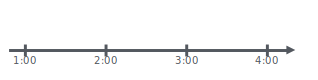
\includegraphics{DataHora/images/timeline01.png}

\begin{Shaded}
\begin{Highlighting}[]
\NormalTok{nor }\OtherTok{\textless{}{-}} \FunctionTok{ymd\_hms}\NormalTok{(}\StringTok{"2018{-}01{-}01 01:30:00"}\NormalTok{,}\AttributeTok{tz=}\StringTok{"US/Eastern"}\NormalTok{) }
\FunctionTok{print}\NormalTok{(nor)}
\end{Highlighting}
\end{Shaded}

\begin{verbatim}
[1] "2018-01-01 01:30:00 EST"
\end{verbatim}

Já, quando o horário de verão se inicia, termos o seguinte cenário na
linha do tempo:

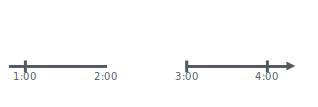
\includegraphics{DataHora/images/timeline02.png}

\begin{Shaded}
\begin{Highlighting}[]
\NormalTok{gap }\OtherTok{\textless{}{-}} \FunctionTok{ymd\_hms}\NormalTok{(}\StringTok{"2018{-}03{-}11 01:30:00"}\NormalTok{,}\AttributeTok{tz=}\StringTok{"US/Eastern"}\NormalTok{)}
\end{Highlighting}
\end{Shaded}

Quando o horário então se encerra, temos na linha do tempo este cenário:

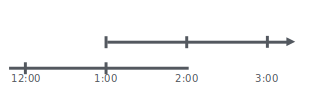
\includegraphics{DataHora/images/timeline03.png}

\begin{Shaded}
\begin{Highlighting}[]
\NormalTok{lap }\OtherTok{\textless{}{-}} \FunctionTok{ymd\_hms}\NormalTok{(}\StringTok{"2018{-}11{-}04 00:30:00"}\NormalTok{,}\AttributeTok{tz=}\StringTok{"US/Eastern"}\NormalTok{)}
\end{Highlighting}
\end{Shaded}

E ainda temos o ``ano-bisexto'', que também causa inconsistência na
linha do tempo:

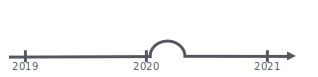
\includegraphics{DataHora/images/timeline04.png}

\begin{Shaded}
\begin{Highlighting}[]
\NormalTok{leap }\OtherTok{\textless{}{-}} \FunctionTok{ymd}\NormalTok{(}\StringTok{"2019{-}03{-}01"}\NormalTok{)}
\end{Highlighting}
\end{Shaded}

Para os casos acima, criamos quarto objetos data e hora: \textbf{nor},
\textbf{gap}, \textbf{lap} e \textbf{leap} para representar cada cenário
de inconsistência na linha do tempo.

Agora veremos com as três classes do lubridate citadas anteriormente
reagem em cada situação:

\hypertarget{peruxedodos}{%
\subsection{\texorpdfstring{\textbf{Períodos}}{Períodos}}\label{peruxedodos}}

Vimos que os períodos acompanham as mudanças no horário do relógio, isto
ignora irregularidades na ``linha do tempo''.

Por exemplo, se quisermos adicionar 90 minutos ao objeto nor criado
anteriormente, teremos:

\begin{Shaded}
\begin{Highlighting}[]
\NormalTok{nor }\SpecialCharTok{+} \FunctionTok{minutes}\NormalTok{(}\DecValTok{90}\NormalTok{)}
\end{Highlighting}
\end{Shaded}

\begin{verbatim}
[1] "2018-01-01 03:00:00 EST"
\end{verbatim}

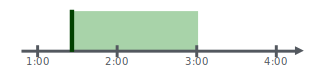
\includegraphics{DataHora/images/period01.png}

Já, se quisermos adicionar 90 minutos no dia do início do horário de
verão (objeto gap), teremos:

\begin{Shaded}
\begin{Highlighting}[]
\NormalTok{gap }\SpecialCharTok{+} \FunctionTok{minutes}\NormalTok{(}\DecValTok{90}\NormalTok{)}
\end{Highlighting}
\end{Shaded}

\begin{verbatim}
[1] "2018-03-11 03:00:00 EDT"
\end{verbatim}

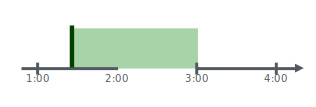
\includegraphics{DataHora/images/period02.png}

Veja que o período ignorou a inconsistência na linha do linha e trouxe o
resultado como ela não existisse.

O mesmo aconteceria com a data e hora do objeto lap criado no fim do
horário de verão:

\begin{Shaded}
\begin{Highlighting}[]
\NormalTok{lap }\SpecialCharTok{+} \FunctionTok{minutes}\NormalTok{(}\DecValTok{90}\NormalTok{)}
\end{Highlighting}
\end{Shaded}

\begin{verbatim}
[1] "2018-11-04 02:00:00 EST"
\end{verbatim}

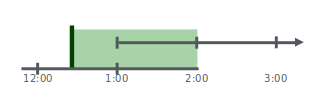
\includegraphics{DataHora/images/period03.png}

Situação identica aconteceria para o objeto leap criado em ano bisexto.
Por exemplo, digamos que queremos somar um período de 1 ano.

\begin{Shaded}
\begin{Highlighting}[]
\NormalTok{leap }\SpecialCharTok{+} \FunctionTok{years}\NormalTok{(}\DecValTok{1}\NormalTok{)}
\end{Highlighting}
\end{Shaded}

\begin{verbatim}
[1] "2020-03-01"
\end{verbatim}

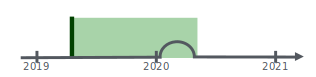
\includegraphics{DataHora/images/period04.png}

As funções de períodos para adicionar ou subtrair data e hora, tem o
nome da unidade seguido de um ``s''. Nos exemplos anterior somamos
minutos usando minutes() e anos usando years().

A lista abaixo traz as funções que criam objetos períodos, ou sejam, que
modelam eventos que acontecem em horário específico do relógio.

Podemos utilzar estes objetos para somar ou subtrair de objetos data ae
hora.

\begin{longtable}[]{@{}ll@{}}
\toprule()
Função & Objeto Período \\
\midrule()
\endhead
years(x = 1) & x anos \\
months(x) & x meses \\
weeks(x = 1) & x semanas \\
days(x = 1) & x dias \\
hours(x = 1) & x horas \\
minutes(x = 1) & x minutos \\
seconds(x = 1) & x segundos \\
milliseconds(x = 1) & x milisegundos \\
microseconds(x = 1) & x microsegundos \\
nanoseconds(x = 1) & x nanosegundos \\
picoseconds(x = 1) & x picosegundos \\
\bottomrule()
\end{longtable}

Por exemplo, se quisermos criar um objeto período com 3 meses e 12 dias,
fazemos:

\begin{Shaded}
\begin{Highlighting}[]
\NormalTok{p }\OtherTok{\textless{}{-}} \FunctionTok{months}\NormalTok{(}\DecValTok{3}\NormalTok{) }\SpecialCharTok{+} \FunctionTok{days}\NormalTok{(}\DecValTok{12}\NormalTok{)}
\NormalTok{p}
\end{Highlighting}
\end{Shaded}

\begin{verbatim}
[1] "3m 12d 0H 0M 0S"
\end{verbatim}

Para subtrair este período de um objeto data e hora, fazemos:

\begin{Shaded}
\begin{Highlighting}[]
\NormalTok{dt }\SpecialCharTok{{-}}\NormalTok{ p}
\end{Highlighting}
\end{Shaded}

\begin{verbatim}
[1] "2017-08-16 12:00:00 UTC"
\end{verbatim}

Podemos também usar as funções abaixo para criar objetos período:

\hypertarget{period}{%
\subsubsection{period}\label{period}}

Use para automatizar a criação de períodos.

Por exemplo, para criar um objeto com período de 5 anos, podemos usar
years(5) ou:

\begin{Shaded}
\begin{Highlighting}[]
\FunctionTok{period}\NormalTok{(}\DecValTok{5}\NormalTok{, }\AttributeTok{unit =} \StringTok{"years"}\NormalTok{)}
\end{Highlighting}
\end{Shaded}

\begin{verbatim}
[1] "5y 0m 0d 0H 0M 0S"
\end{verbatim}

\hypertarget{as.period}{%
\subsubsection{as.period}\label{as.period}}

Use para transformar objetos de duração, intervalos e números para
obejtos do tipo período:

Por exemplos, temos um número 5 e queremos criar um período de 5 dias,
podemos fazer:

\begin{Shaded}
\begin{Highlighting}[]
\FunctionTok{as.period}\NormalTok{(}\DecValTok{5}\NormalTok{, }\AttributeTok{unit=}\StringTok{"days"}\NormalTok{)}
\end{Highlighting}
\end{Shaded}

\begin{verbatim}
[1] "5d 0H 0M 0S"
\end{verbatim}

\hypertarget{period_to_seconds}{%
\subsubsection{period\_to\_seconds}\label{period_to_seconds}}

Use para transformar um objeto do tipo período no total de número de
segundos do período:

\begin{Shaded}
\begin{Highlighting}[]
\FunctionTok{period\_to\_seconds}\NormalTok{(p)}
\end{Highlighting}
\end{Shaded}

\begin{verbatim}
[1] 8926200
\end{verbatim}

\hypertarget{durauxe7uxe3o}{%
\subsection{\texorpdfstring{\textbf{Duração}}{Duração}}\label{durauxe7uxe3o}}

Diferentes dos objetos períodos, os objetos do tipo duração
(\emph{duration}), Acompanham a passagem do ``tempo físico'', o que
diverge do horário do relógio quando irregularidades na ``linha do
tempo'' acontecem.

Por exemplo, digamos que temos nosso ``dia normal'' na linha do tempo e
adicionarmos 90 minutos de duração:

\begin{Shaded}
\begin{Highlighting}[]
\NormalTok{nor }\SpecialCharTok{+} \FunctionTok{dminutes}\NormalTok{(}\DecValTok{90}\NormalTok{)}
\end{Highlighting}
\end{Shaded}

\begin{verbatim}
[1] "2018-01-01 03:00:00 EST"
\end{verbatim}

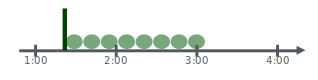
\includegraphics{DataHora/images/duration01.png}

Até aqui, o resultado foi similar à adicionarmos um objeto do tipo
período de 90 minutes.

Porém, veja o que acontece quando temos uma inconsistência na linha do
tempo, como por exemplo nosso início de horário de verão em nosso objeto
gap.

\begin{Shaded}
\begin{Highlighting}[]
\NormalTok{gap }\SpecialCharTok{+} \FunctionTok{dminutes}\NormalTok{(}\DecValTok{90}\NormalTok{)}
\end{Highlighting}
\end{Shaded}

\begin{verbatim}
[1] "2018-03-11 04:00:00 EDT"
\end{verbatim}

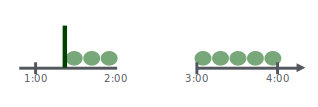
\includegraphics{DataHora/images/duration02.png}

O mesmo acontece com nosso término de horário de verão em nosso objeto
lap:

\begin{Shaded}
\begin{Highlighting}[]
\NormalTok{lap }\SpecialCharTok{+} \FunctionTok{dminutes}\NormalTok{(}\DecValTok{90}\NormalTok{)}
\end{Highlighting}
\end{Shaded}

\begin{verbatim}
[1] "2018-11-04 01:00:00 EST"
\end{verbatim}

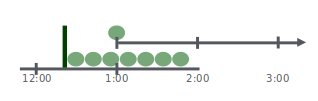
\includegraphics{DataHora/images/duration03.png}

Ou mesmo com nosso ano bi-sexto:

\begin{Shaded}
\begin{Highlighting}[]
\NormalTok{leap}
\end{Highlighting}
\end{Shaded}

\begin{verbatim}
[1] "2019-03-01"
\end{verbatim}

\begin{Shaded}
\begin{Highlighting}[]
\NormalTok{leap }\SpecialCharTok{+} \FunctionTok{dyears}\NormalTok{(}\DecValTok{1}\NormalTok{)}
\end{Highlighting}
\end{Shaded}

\begin{verbatim}
[1] "2020-02-29 06:00:00 UTC"
\end{verbatim}

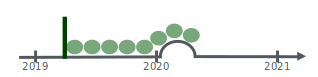
\includegraphics{DataHora/images/duration04.png}

Podemos pensar em objetos de duração como um modelo físico, como uma
vida útil de uma bateria. As durações são armazenados como segundos, que
é a única unidade distância consistente.

Por exemplo, se criarmos um objeto duração equivalente à 14 dias, ele
irá armazenar 1209600s.

\begin{Shaded}
\begin{Highlighting}[]
\NormalTok{dd }\OtherTok{\textless{}{-}} \FunctionTok{ddays}\NormalTok{(}\DecValTok{14}\NormalTok{)}
\NormalTok{dd}
\end{Highlighting}
\end{Shaded}

\begin{verbatim}
[1] "1209600s (~2 weeks)"
\end{verbatim}

\begin{tcolorbox}[enhanced jigsaw, rightrule=.15mm, arc=.35mm, coltitle=black, colframe=quarto-callout-tip-color-frame, opacityback=0, toprule=.15mm, left=2mm, breakable, colback=white, bottomtitle=1mm, leftrule=.75mm, title=\textcolor{quarto-callout-tip-color}{\faLightbulb}\hspace{0.5em}{Dica}, colbacktitle=quarto-callout-tip-color!10!white, titlerule=0mm, bottomrule=.15mm, toptitle=1mm, opacitybacktitle=0.6]
Há também uma classe chamada ``\textbf{difftime}'', que se encontra no R
base, ou seja, fora do pacote lubridate, usada para lidar com durações
de tempo.
\end{tcolorbox}

As funções para criar objetos de duração, são similares às dos objetos
períodos, porém se iniciam com a letra ``d'', veja:

\begin{longtable}[]{@{}ll@{}}
\caption{Podemos também usar as funções abaixo para criar objetos
duração:}\tabularnewline
\toprule()
Função & Objeto Duração \\
\midrule()
\endfirsthead
\toprule()
Função & Objeto Duração \\
\midrule()
\endhead
dyears(x = 1) & 31536000x anos \\
dmonths(x) & 2629800x meses \\
dweeks(x = 1) & 604800x semanas \\
ddays(x = 1) & x86400x dias \\
dhours(x = 1) & 3600x horas \\
dminutes(x = 1) & 60x minutos \\
dseconds(x = 1) & x segundos \\
dmilliseconds(x = 1) & x X \(10^3\) milisegundos \\
dmicroseconds(x = 1) & x X \(10^6\) microsegundos \\
dnanoseconds(x = 1) & x X \(10^9\) nanosegundos \\
dpicoseconds(x = 1) & x X \(10 ^{12}\)picosegundos \\
\bottomrule()
\end{longtable}

\hypertarget{duration}{%
\subsubsection{duration}\label{duration}}

Use para automatizar a criação de durações.

Por exemplo, para criar um objeto com duração de 5 anos, podemos usar
dyears(5) ou:

\begin{Shaded}
\begin{Highlighting}[]
\FunctionTok{duration}\NormalTok{(}\DecValTok{5}\NormalTok{, }\AttributeTok{unit =} \StringTok{"years"}\NormalTok{)}
\end{Highlighting}
\end{Shaded}

\begin{verbatim}
[1] "157788000s (~5 years)"
\end{verbatim}

\hypertarget{as.duration}{%
\subsubsection{as.duration}\label{as.duration}}

Use para transformar objetos de períodos, intervalos e números para
objetos do tipo duração:

Por exemplos, temos um número 10 e queremos criar um período de 10
segundos, podemos fazer:

\begin{Shaded}
\begin{Highlighting}[]
\FunctionTok{as.duration}\NormalTok{(}\DecValTok{10}\NormalTok{)}
\end{Highlighting}
\end{Shaded}

\begin{verbatim}
[1] "10s"
\end{verbatim}

\hypertarget{make_difftime}{%
\subsubsection{make\_difftime}\label{make_difftime}}

Use para criar um objeto difftime (R base) com um número específico de
unidades.

\begin{Shaded}
\begin{Highlighting}[]
\FunctionTok{make\_difftime}\NormalTok{(}\DecValTok{3600}\NormalTok{)}
\end{Highlighting}
\end{Shaded}

\begin{verbatim}
Time difference of 1 hours
\end{verbatim}

\hypertarget{intervalo}{%
\subsection{\texorpdfstring{\textbf{Intervalo}}{Intervalo}}\label{intervalo}}

Objeto do tipo intervalo, representam um intervalo específico da ``linha
do tempo'', limitado pelo início e fim da data e hora. Se dividirmor o
intervalo, pela pela duração teremos a distância física do tempo. Se
dividirmos o intervalo pelo período, termeos a distância relativa ao
relógio.

Podemos criar um objeto de intervalo, usando a função interval() ou o
símbolo \%-\/-\%.

\begin{Shaded}
\begin{Highlighting}[]
\NormalTok{i }\OtherTok{\textless{}{-}} \FunctionTok{interval}\NormalTok{(}\FunctionTok{ymd}\NormalTok{(}\StringTok{"2017{-}01{-}01"}\NormalTok{), d)}
\NormalTok{j }\OtherTok{\textless{}{-}}\NormalTok{ d }\SpecialCharTok{\%{-}{-}\%} \FunctionTok{ymd}\NormalTok{(}\StringTok{"2017{-}12{-}31"}\NormalTok{)}
\NormalTok{i; j}
\end{Highlighting}
\end{Shaded}

\begin{verbatim}
[1] 2017-01-01 UTC--2017-11-01 UTC
\end{verbatim}

\begin{verbatim}
[1] 2017-11-01 UTC--2017-12-31 UTC
\end{verbatim}

Observe pelo resultado acima, temos duas data para cada objeto, a da
esquerda representa o início do intervalo e a da direito o fim.

Por exemplo, vamos pegar um dia normal na linha do tempo, representado
pelo objeto nor e definirmos como o início do intervalo, e para o fim do
intervalo usaremos nor mais um período de 90 minutos.

\begin{Shaded}
\begin{Highlighting}[]
\FunctionTok{interval}\NormalTok{(nor, nor }\SpecialCharTok{+} \FunctionTok{minutes}\NormalTok{(}\DecValTok{90}\NormalTok{))}
\end{Highlighting}
\end{Shaded}

\begin{verbatim}
[1] 2018-01-01 01:30:00 EST--2018-01-01 03:00:00 EST
\end{verbatim}

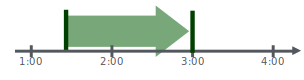
\includegraphics{DataHora/images/interval01.png}

Agora, em uma linha do tempo inconsistente, o intervalo se mantém
alinhado com o relógio. Veja como fica quando adicionamos um intervalo
de 90 minutos quando temos o início de um horário de verão:

\begin{Shaded}
\begin{Highlighting}[]
\FunctionTok{interval}\NormalTok{(gap, gap}\SpecialCharTok{+}\FunctionTok{minutes}\NormalTok{(}\DecValTok{90}\NormalTok{))}
\end{Highlighting}
\end{Shaded}

\begin{verbatim}
[1] 2018-03-11 01:30:00 EST--2018-03-11 03:00:00 EDT
\end{verbatim}

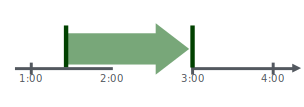
\includegraphics{DataHora/images/interval02.png}

De forma similar, ocorre quando temos um intervalo quando há o término
de um horário de verão:

\begin{Shaded}
\begin{Highlighting}[]
\FunctionTok{interval}\NormalTok{(lap, lap}\SpecialCharTok{+}\FunctionTok{minutes}\NormalTok{(}\DecValTok{90}\NormalTok{))}
\end{Highlighting}
\end{Shaded}

\begin{verbatim}
[1] 2018-11-04 00:30:00 EDT--2018-11-04 02:00:00 EST
\end{verbatim}

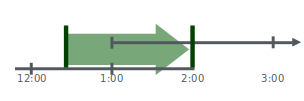
\includegraphics{DataHora/images/interval03.png}

Ou mesmo quando temos um intervalo em um ano bi-sexto:

\begin{Shaded}
\begin{Highlighting}[]
\FunctionTok{interval}\NormalTok{(leap, leap }\SpecialCharTok{+} \FunctionTok{years}\NormalTok{(}\DecValTok{1}\NormalTok{))}
\end{Highlighting}
\end{Shaded}

\begin{verbatim}
[1] 2019-03-01 UTC--2020-03-01 UTC
\end{verbatim}

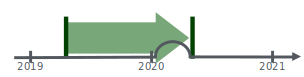
\includegraphics{DataHora/images/interval04.png}

O pacote lubridate possui diversas funções para lidar com intervalo.

\hypertarget{within}{%
\subsubsection{\%within\%}\label{within}}

Use para identificar se um objeto do tipo intervalo ou data e hora ``a''
cai dentro de um interválo ``b''

Por exemplo, se quisermos se a data e hora atual está dentro do
intervalo ``i''.

\begin{Shaded}
\begin{Highlighting}[]
\FunctionTok{now}\NormalTok{ () }\SpecialCharTok{\%within\%}\NormalTok{ i}
\end{Highlighting}
\end{Shaded}

\begin{verbatim}
[1] FALSE
\end{verbatim}

\hypertarget{int_start}{%
\subsubsection{int\_start}\label{int_start}}

Use para obter ou definir o \textbf{início} de um \textbf{intervalo}:

\begin{Shaded}
\begin{Highlighting}[]
\FunctionTok{int\_start}\NormalTok{(i)}
\end{Highlighting}
\end{Shaded}

\begin{verbatim}
[1] "2017-01-01 UTC"
\end{verbatim}

\begin{Shaded}
\begin{Highlighting}[]
\FunctionTok{int\_start}\NormalTok{(i) }\OtherTok{\textless{}{-}} \FunctionTok{now}\NormalTok{()}
\end{Highlighting}
\end{Shaded}

\begin{tcolorbox}[enhanced jigsaw, rightrule=.15mm, arc=.35mm, coltitle=black, colframe=quarto-callout-note-color-frame, opacityback=0, toprule=.15mm, left=2mm, breakable, colback=white, bottomtitle=1mm, leftrule=.75mm, title=\textcolor{quarto-callout-note-color}{\faInfo}\hspace{0.5em}{Nota}, colbacktitle=quarto-callout-note-color!10!white, titlerule=0mm, bottomrule=.15mm, toptitle=1mm, opacitybacktitle=0.6]
A função int\_end() faz o oposto, ou seja, obtem ou define o
\textbf{fim} de um intervalo.
\end{tcolorbox}

int\_aligns

Use para identificar se dois objetos do tipo intervalo estão alinhados,
ou seja, compartilham de uma mesma data e hora.

\begin{Shaded}
\begin{Highlighting}[]
\FunctionTok{int\_aligns}\NormalTok{(i,j)}
\end{Highlighting}
\end{Shaded}

\begin{verbatim}
[1] TRUE
\end{verbatim}

No exemplo acima, temos ``2017-11-28'' como início de um objeto e fim de
outro, por isso dizemos que eles estão alinhados.

\begin{tcolorbox}[enhanced jigsaw, rightrule=.15mm, arc=.35mm, coltitle=black, colframe=quarto-callout-note-color-frame, opacityback=0, toprule=.15mm, left=2mm, breakable, colback=white, bottomtitle=1mm, leftrule=.75mm, title=\textcolor{quarto-callout-note-color}{\faInfo}\hspace{0.5em}{Nota}, colbacktitle=quarto-callout-note-color!10!white, titlerule=0mm, bottomrule=.15mm, toptitle=1mm, opacitybacktitle=0.6]
Se quisermos saber se estes objetos estão \textbf{sobrepostos}, ou seja,
tem partes de uma intervá-lo que também fazem parte de outro, utilizamos
a função \textbf{int\_overlaps}().
\end{tcolorbox}

\hypertarget{int_diff}{%
\subsubsection{int\_diff}\label{int_diff}}

Use para transformar em intervalos, os valores que estão em um vetor de
data e hora.

\begin{Shaded}
\begin{Highlighting}[]
\NormalTok{v }\OtherTok{\textless{}{-}} \FunctionTok{c}\NormalTok{(dt, dt}\SpecialCharTok{+}\DecValTok{100}\NormalTok{, dt}\SpecialCharTok{+}\DecValTok{1000}\NormalTok{); }\FunctionTok{int\_diff}\NormalTok{(v)}
\end{Highlighting}
\end{Shaded}

\begin{verbatim}
[1] 2017-11-28 12:00:00 UTC--2017-11-28 12:01:40 UTC
[2] 2017-11-28 12:01:40 UTC--2017-11-28 12:16:40 UTC
\end{verbatim}

int\_flip

Use para colocar em ordem reversa a direção de um intervalo, ou seja, a
dat e hora do fim vai para o início do intervalo e a data e hora do
início vai para o final.

\begin{Shaded}
\begin{Highlighting}[]
\FunctionTok{int\_flip}\NormalTok{(i)}
\end{Highlighting}
\end{Shaded}

\begin{verbatim}
[1] 2017-11-01 UTC--2022-09-12 14:19:17 UTC
\end{verbatim}

Para colocar em ordem padrão um intervalo de acordo com a linha do
tempo, podemos usar a função \textbf{int\_standardize}().

\begin{Shaded}
\begin{Highlighting}[]
\FunctionTok{int\_standardize}\NormalTok{(i)}
\end{Highlighting}
\end{Shaded}

\begin{verbatim}
[1] 2017-11-01 UTC--2022-09-12 14:19:17 UTC
\end{verbatim}

\hypertarget{int_length}{%
\subsubsection{int\_length}\label{int_length}}

Use para obter, em segundos, o tempo total de um intervalo:

\begin{Shaded}
\begin{Highlighting}[]
\FunctionTok{int\_length}\NormalTok{(i)}
\end{Highlighting}
\end{Shaded}

\begin{verbatim}
[1] -153497958
\end{verbatim}

\hypertarget{int_shift}{%
\subsubsection{int\_shift}\label{int_shift}}

Use para mover um intervalo para mais ou para menos na linha do tempo.

Por exemplo, se mover todo o intervalo (início e fim) em um dia antes da
linha do tempo, podemos fazer:

\begin{Shaded}
\begin{Highlighting}[]
\FunctionTok{int\_shift}\NormalTok{(i, }\FunctionTok{days}\NormalTok{(}\SpecialCharTok{{-}}\DecValTok{1}\NormalTok{))}
\end{Highlighting}
\end{Shaded}

\begin{verbatim}
[1] 2022-09-11 11:19:17 -03--2017-10-30 22:00:00 -02
\end{verbatim}

\hypertarget{as.interval}{%
\subsubsection{as.interval}\label{as.interval}}

Use para criar um objeto intervalo com determinado periodo definindo uma
dat e hora de início.

Por exemplo, para criarmos um intervalo de 1 dia, iniciando na data
atual, podemos fazer:

\begin{Shaded}
\begin{Highlighting}[]
\FunctionTok{as.interval}\NormalTok{(}\FunctionTok{days}\NormalTok{(}\DecValTok{1}\NormalTok{), }\AttributeTok{start =} \FunctionTok{now}\NormalTok{())}
\end{Highlighting}
\end{Shaded}

\begin{verbatim}
[1] 2022-09-12 11:19:18 -03--2022-09-13 11:19:18 -03
\end{verbatim}

\begin{tcolorbox}[enhanced jigsaw, rightrule=.15mm, arc=.35mm, coltitle=black, colframe=quarto-callout-note-color-frame, opacityback=0, toprule=.15mm, left=2mm, breakable, colback=white, bottomtitle=1mm, leftrule=.75mm, title=\textcolor{quarto-callout-note-color}{\faInfo}\hspace{0.5em}{Nota}, colbacktitle=quarto-callout-note-color!10!white, titlerule=0mm, bottomrule=.15mm, toptitle=1mm, opacitybacktitle=0.6]
Podemos usar a função \textbf{is.interval}() para saber se um objeto é
um intervalo válido ou não.
\end{tcolorbox}

\hypertarget{datas-imaginuxe1rias}{%
\section{Datas Imaginárias}\label{datas-imaginuxe1rias}}

É importante observar que nem todos os anos tem 365 dias (ex: ano
bi-sexto) e nem todos os minutos tem 60 segundos (ex: fim de horário de
verão).

Isso é importante de ser observado, pois em alguns casos tentamos criar
data imaginárias, como por exemplo ``Fev 31'', adicionando um mês à
``Jan 31''. As funções do pacote lubridate são inteligentes o suficiente
e neste caso retornaria um valor NA:\\

\begin{Shaded}
\begin{Highlighting}[]
\NormalTok{jan31 }\OtherTok{\textless{}{-}} \FunctionTok{ymd}\NormalTok{(}\DecValTok{20180131}\NormalTok{)}
\NormalTok{jan31 }\SpecialCharTok{+} \FunctionTok{months}\NormalTok{(}\DecValTok{1}\NormalTok{)}
\end{Highlighting}
\end{Shaded}

\begin{verbatim}
[1] NA
\end{verbatim}

\hypertarget{aritmuxe9tica-dos-meses}{%
\subsection{Aritmética dos meses}\label{aritmuxe9tica-dos-meses}}

Porém, as vezes, intuitivamente, é isto que desejamos fazer, ou seja,
adicionar ``um mês'' a ``Jan 31'', mas que a função seja inteligente o
suficiente para \textbf{rolar} para o \textbf{último} \textbf{dia}
\textbf{do} \textbf{mês}.

Adicionar ou subtrair \textbf{meses} as vezes é uma tarefa difícil, pois
temos meses de diferentes tamanhos (ex: 30, 31, 28 dias ou até 29). Por
isso, em alguns casos é útil termos a possibildade de fazermos um
ajustes automáticos.

Para isso usamos, ao invés do sinal de adição ``\textbf{+}'', utilizamos
o símbolo \%\textbf{m+}\% para adicionar meses (ou \%\textbf{m-}\% para
subtrair). Veja:

\begin{Shaded}
\begin{Highlighting}[]
\NormalTok{jan31 }\SpecialCharTok{\%m+\%} \FunctionTok{months}\NormalTok{(}\DecValTok{1}\NormalTok{)}
\end{Highlighting}
\end{Shaded}

\begin{verbatim}
[1] "2018-02-28"
\end{verbatim}

A função \textbf{add\_with\_rollback}() nos permite rolar a data da soma
para o primeiro dia do mês seguinte (e não o último dia do mês anterior)
usando o argumento \textbf{roll\_to\_first.}

\begin{Shaded}
\begin{Highlighting}[]
\FunctionTok{add\_with\_rollback}\NormalTok{(jan31, }\FunctionTok{months}\NormalTok{(}\DecValTok{1}\NormalTok{), }\AttributeTok{roll\_to\_first =} \ConstantTok{TRUE}\NormalTok{)}
\end{Highlighting}
\end{Shaded}

\begin{verbatim}
[1] "2018-03-01"
\end{verbatim}

\hypertarget{programauxe7uxe3o-funcional-com-purrr}{%
\chapter{Programação Funcional com
PURRR}\label{programauxe7uxe3o-funcional-com-purrr}}

\hypertarget{introduuxe7uxe3o-10}{%
\section{Introdução}\label{introduuxe7uxe3o-10}}

A seguir temos uma série de facildades que o pacote PURRR do R trás para
trabalharmos com listas, funções e um paradigma de programação
funcional.

Para saber mais sobre este pacote, acesse:

\url{https://cran.r-project.org/package=purr}.

\begin{tcolorbox}[enhanced jigsaw, rightrule=.15mm, arc=.35mm, coltitle=black, colframe=quarto-callout-warning-color-frame, opacityback=0, toprule=.15mm, left=2mm, breakable, colback=white, bottomtitle=1mm, leftrule=.75mm, title=\textcolor{quarto-callout-warning-color}{\faExclamationTriangle}\hspace{0.5em}{Aviso}, colbacktitle=quarto-callout-warning-color!10!white, titlerule=0mm, bottomrule=.15mm, toptitle=1mm, opacitybacktitle=0.6]
Para melhor utilizar este material, é importante que você tenha uma
introdução à linguagem R e saiba carregar pacotes (packages) no R. Para
mais informações acesse:

\url{https://education.rstudio.com/learn/beginner/}.
\end{tcolorbox}

Para os exemplos, iremos carregar o seguinte pacote:

\begin{itemize}
\tightlist
\item
  \textbf{tidyverse}
\end{itemize}

\begin{Shaded}
\begin{Highlighting}[]
\FunctionTok{library}\NormalTok{ (tidyverse)}
\end{Highlighting}
\end{Shaded}

\hypertarget{exemplos-da-folha-de-referuxeancia-6}{%
\subsection{Exemplos da Folha de
Referência}\label{exemplos-da-folha-de-referuxeancia-6}}

A maioria dos exemplos, visam ajudar na interpretação dos exemplos e
funções encontradas na
\href{https://github.com/scopinho/R-cheatsheets/blob/main/translations/portuguese/factors_pt_br.pdf}{\textbf{Folha
de Referência}} do purrr disponível no site do
\href{rstudio.com}{RStudio}.

\href{images/cs-purrr-01.png}{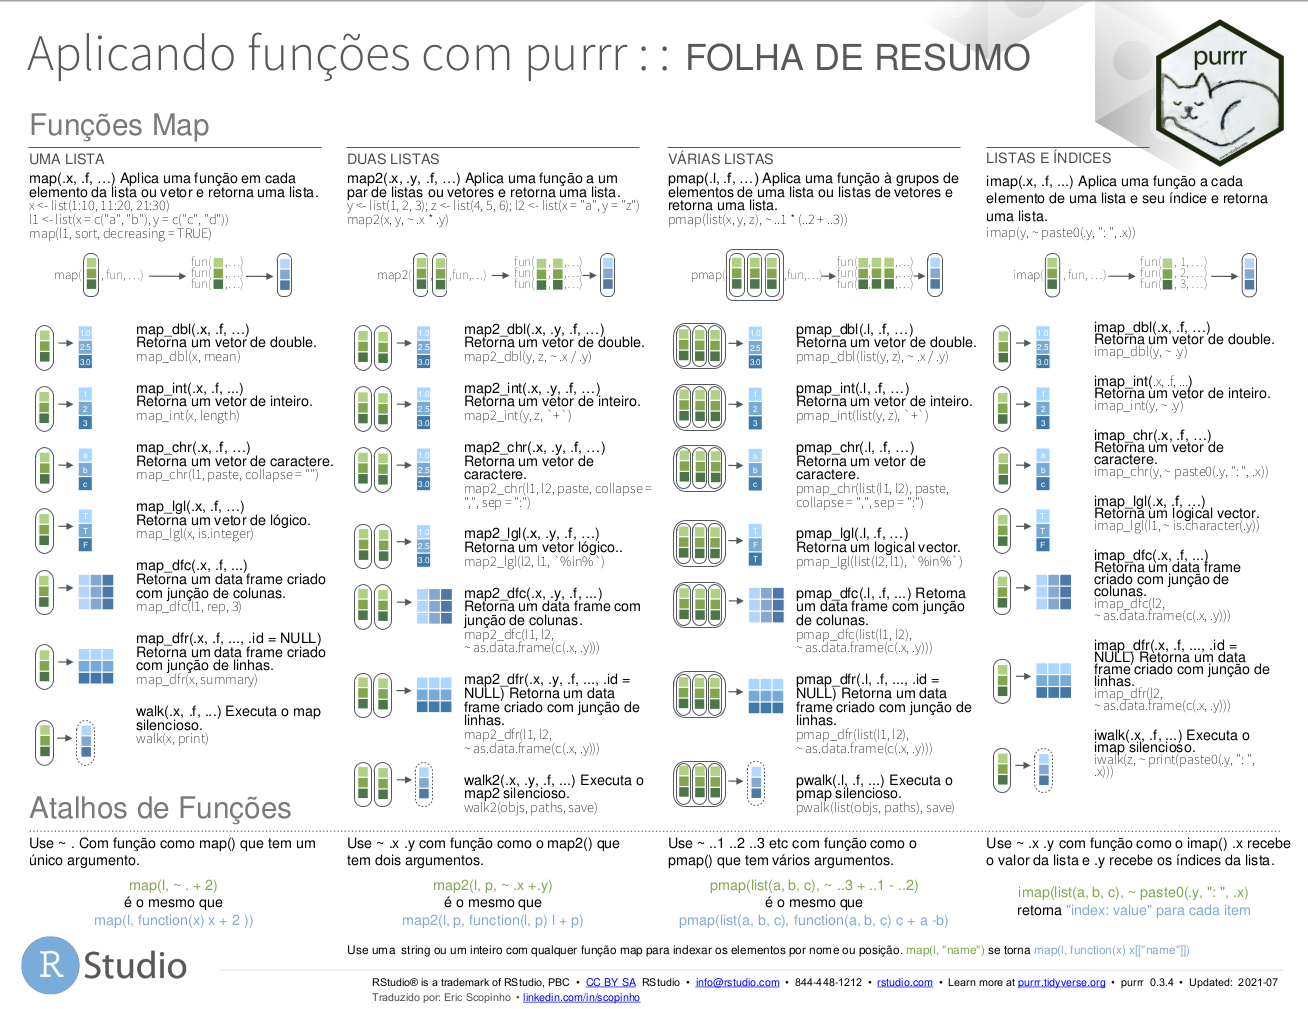
\includegraphics[width=5.39583in,height=\textheight]{Funcional/images/cs-purrr-01.png}}
\href{images/cs-purrr-02.png}{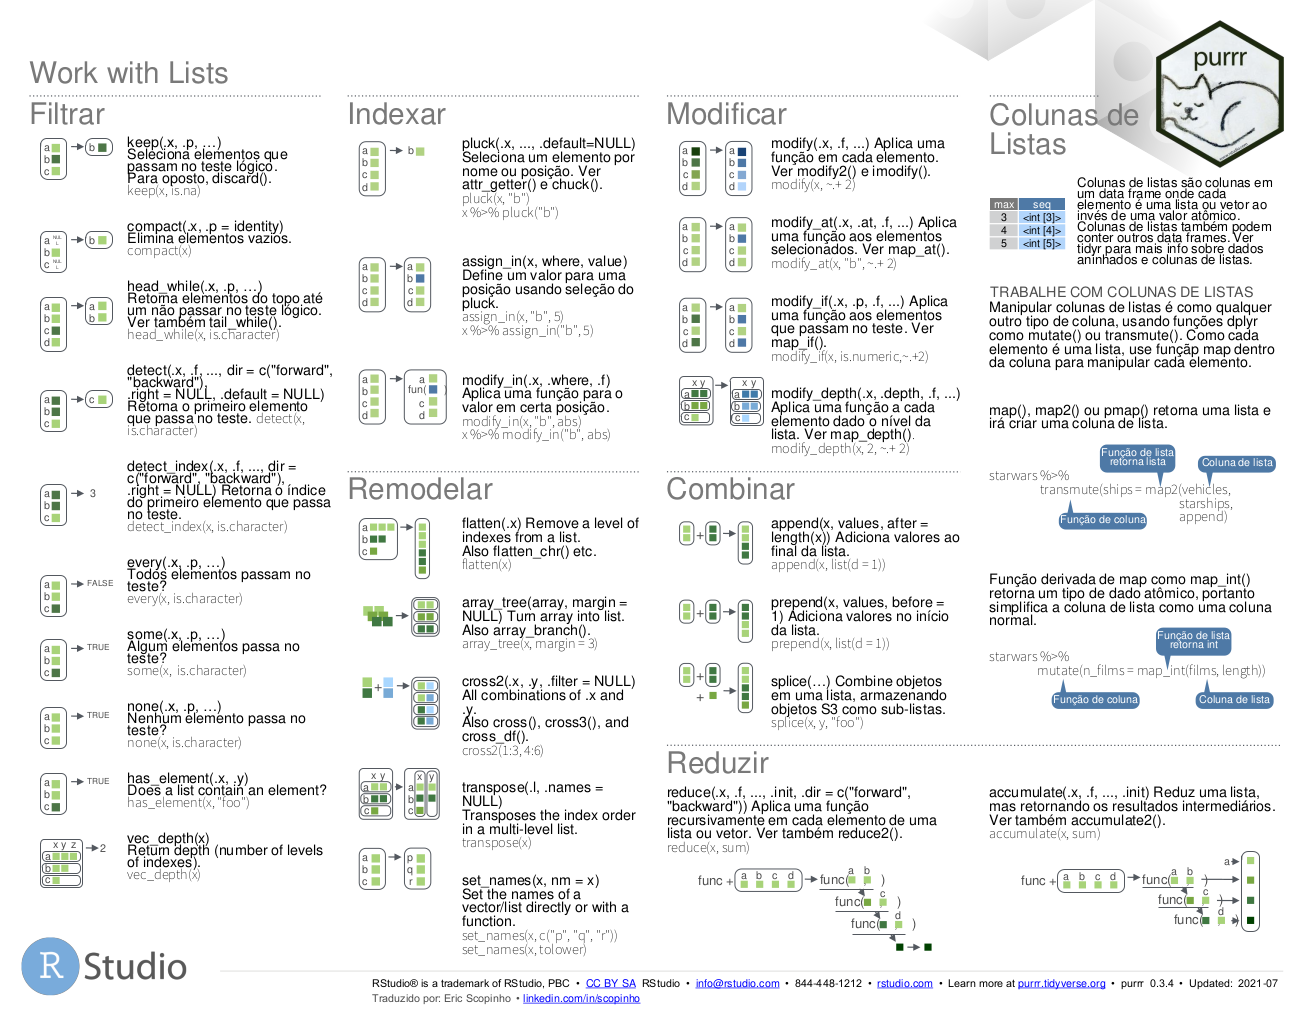
\includegraphics[width=5.39583in,height=\textheight]{Funcional/images/cs-purrr-02.png}}

\begin{center}\rule{0.5\linewidth}{0.5pt}\end{center}

\hypertarget{programauxe7uxe3o-funcional}{%
\section{Programação Funcional}\label{programauxe7uxe3o-funcional}}

Programação funcional é um paradigma de programação onde aplicações são
construídas aplicando uma composição de funções. É um paradigma de
programação declarativa, onde definições de funções são árvores de
expressão que mapeam um valor para outro valor, ao invés de comandos
imperativos que mudam o estado do programa.

Para tentar deixar este tema mais simplificado, vamos imaginar um
cenário bem simples on você já está familiarizado com algumas funções do
R e decide começar a utilizá-lo. Após um certo tempo, chegará a
conclusão que muitas vezes ao trabalhar com dados, precisamos utilizar a
mesma função com alguns parêmtros diferentes para concluirmos nossa
análise.

Dentro dessa ideia básica, digamos que precise da \textbf{média e valor
máximo} da variável peso (\textbf{wt}) da base de dados \textbf{mtcars}:

\begin{Shaded}
\begin{Highlighting}[]
\NormalTok{mtcars}
\end{Highlighting}
\end{Shaded}

\begin{verbatim}
                     mpg cyl  disp  hp drat    wt  qsec vs am gear carb
Mazda RX4           21.0   6 160.0 110 3.90 2.620 16.46  0  1    4    4
Mazda RX4 Wag       21.0   6 160.0 110 3.90 2.875 17.02  0  1    4    4
Datsun 710          22.8   4 108.0  93 3.85 2.320 18.61  1  1    4    1
Hornet 4 Drive      21.4   6 258.0 110 3.08 3.215 19.44  1  0    3    1
Hornet Sportabout   18.7   8 360.0 175 3.15 3.440 17.02  0  0    3    2
Valiant             18.1   6 225.0 105 2.76 3.460 20.22  1  0    3    1
Duster 360          14.3   8 360.0 245 3.21 3.570 15.84  0  0    3    4
Merc 240D           24.4   4 146.7  62 3.69 3.190 20.00  1  0    4    2
Merc 230            22.8   4 140.8  95 3.92 3.150 22.90  1  0    4    2
Merc 280            19.2   6 167.6 123 3.92 3.440 18.30  1  0    4    4
Merc 280C           17.8   6 167.6 123 3.92 3.440 18.90  1  0    4    4
Merc 450SE          16.4   8 275.8 180 3.07 4.070 17.40  0  0    3    3
Merc 450SL          17.3   8 275.8 180 3.07 3.730 17.60  0  0    3    3
Merc 450SLC         15.2   8 275.8 180 3.07 3.780 18.00  0  0    3    3
Cadillac Fleetwood  10.4   8 472.0 205 2.93 5.250 17.98  0  0    3    4
Lincoln Continental 10.4   8 460.0 215 3.00 5.424 17.82  0  0    3    4
Chrysler Imperial   14.7   8 440.0 230 3.23 5.345 17.42  0  0    3    4
Fiat 128            32.4   4  78.7  66 4.08 2.200 19.47  1  1    4    1
Honda Civic         30.4   4  75.7  52 4.93 1.615 18.52  1  1    4    2
Toyota Corolla      33.9   4  71.1  65 4.22 1.835 19.90  1  1    4    1
Toyota Corona       21.5   4 120.1  97 3.70 2.465 20.01  1  0    3    1
Dodge Challenger    15.5   8 318.0 150 2.76 3.520 16.87  0  0    3    2
AMC Javelin         15.2   8 304.0 150 3.15 3.435 17.30  0  0    3    2
Camaro Z28          13.3   8 350.0 245 3.73 3.840 15.41  0  0    3    4
Pontiac Firebird    19.2   8 400.0 175 3.08 3.845 17.05  0  0    3    2
Fiat X1-9           27.3   4  79.0  66 4.08 1.935 18.90  1  1    4    1
Porsche 914-2       26.0   4 120.3  91 4.43 2.140 16.70  0  1    5    2
Lotus Europa        30.4   4  95.1 113 3.77 1.513 16.90  1  1    5    2
Ford Pantera L      15.8   8 351.0 264 4.22 3.170 14.50  0  1    5    4
Ferrari Dino        19.7   6 145.0 175 3.62 2.770 15.50  0  1    5    6
Maserati Bora       15.0   8 301.0 335 3.54 3.570 14.60  0  1    5    8
Volvo 142E          21.4   4 121.0 109 4.11 2.780 18.60  1  1    4    2
\end{verbatim}

Para isso poderíamos fazer:

\begin{Shaded}
\begin{Highlighting}[]
\FunctionTok{mean}\NormalTok{ (mtcars}\SpecialCharTok{$}\NormalTok{wt)}
\end{Highlighting}
\end{Shaded}

\begin{verbatim}
[1] 3.21725
\end{verbatim}

\begin{Shaded}
\begin{Highlighting}[]
\FunctionTok{sd}\NormalTok{ (mtcars}\SpecialCharTok{$}\NormalTok{wt)}
\end{Highlighting}
\end{Shaded}

\begin{verbatim}
[1] 0.9784574
\end{verbatim}

Depois, você acaba precisando da \textbf{média} e \textbf{valor áximo}
para outra variável, digmos potencia (\textbf{hp}) e depois para consumo
(\textbf{mpg}).

\begin{Shaded}
\begin{Highlighting}[]
\FunctionTok{mean}\NormalTok{ (mtcars}\SpecialCharTok{$}\NormalTok{hp)}
\end{Highlighting}
\end{Shaded}

\begin{verbatim}
[1] 146.6875
\end{verbatim}

\begin{Shaded}
\begin{Highlighting}[]
\FunctionTok{sd}\NormalTok{ (mtcars}\SpecialCharTok{$}\NormalTok{hp)}
\end{Highlighting}
\end{Shaded}

\begin{verbatim}
[1] 68.56287
\end{verbatim}

\begin{Shaded}
\begin{Highlighting}[]
\FunctionTok{mean}\NormalTok{ (mtcars}\SpecialCharTok{$}\NormalTok{mpg)}
\end{Highlighting}
\end{Shaded}

\begin{verbatim}
[1] 20.09062
\end{verbatim}

\begin{Shaded}
\begin{Highlighting}[]
\FunctionTok{sd}\NormalTok{ (mtcars}\SpecialCharTok{$}\NormalTok{mpg)}
\end{Highlighting}
\end{Shaded}

\begin{verbatim}
[1] 6.026948
\end{verbatim}

Veja que com simples funções como estas de média (mean) e valor máximo
(max), seu código já está ficando \textbf{repetitivo} e com várias
\textbf{replicações}.

É exatamente para este e alguns outros desafios, que o pacote purr vem
ajudar. Ele, entre outras coisas, ajuda na redução de linhas similares
de código, aplicando funções à conjuntos de dados, diminuindo as
replicações de código e o deixando com maior entendimento.

\hypertarget{mapeando-funuxe7uxf5es}{%
\section{Mapeando funções}\label{mapeando-funuxe7uxf5es}}

No pacote purrr, existem diversas funções que ajudam a \textbf{mapear}
outras funções, onde ao receber uma, duas ou mais listas, iremos aplicar
a mesma função para cada uma delas. Veremos à seguir como devemos
proceder para estes cenários.

\hypertarget{uma-lista}{%
\subsection{Uma lista}\label{uma-lista}}

Seguindo o simples caso da \textbf{média} visto há pouco, poderíamos
usar uma função de \textbf{mapeamento} (\textbf{map}) para aplicar as
funções \textbf{mean}() e \textbf{sd}() para diversos items de uma lista
e retornar um vetor de mesmo tamanho da lista. Nossa lista, pode conter
o valor da variável \textbf{wt}, \textbf{hp}, \textbf{mpg} e muitas
outras, mantendo-se com um código mais enxuto.

Então, em resumo, a função map, recebe uma lista de valores, aplica um
função a ser definida e retorna uma lista com o mesmo tamanho da lista
de entrada.

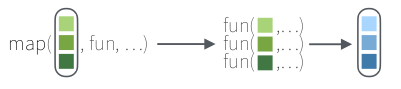
\includegraphics{Funcional/images/map.png}

Veja como ficaria nosso exemplo das \textbf{médias} e \textbf{valor
máximo} com a função \textbf{map}():

\begin{Shaded}
\begin{Highlighting}[]
\CommentTok{\#Cria uma lista para a entrada}
\NormalTok{lista }\OtherTok{\textless{}{-}} \FunctionTok{list}\NormalTok{(}\StringTok{"wt"}\OtherTok{=}\NormalTok{mtcars}\SpecialCharTok{$}\NormalTok{wt, }\StringTok{"hp"}\OtherTok{=}\NormalTok{mtcars}\SpecialCharTok{$}\NormalTok{hp, }\StringTok{"mpg"}\OtherTok{=}\NormalTok{mtcars}\SpecialCharTok{$}\NormalTok{mpg)}

\CommentTok{\#Cria um mapeamento da lista e a função que iremos executar para cada elemento da lista.}

\NormalTok{media }\OtherTok{\textless{}{-}} \FunctionTok{map}\NormalTok{(lista, mean)}
\NormalTok{maximo }\OtherTok{\textless{}{-}} \FunctionTok{map}\NormalTok{(lista, max)}
\end{Highlighting}
\end{Shaded}

Veja que se precisarmos a fazer a \textbf{média} e \textbf{valor máximo}
para 10 novas variáveis, precisamos apenas incluí-las na lista e nenhuma
outra alteração no código seria necessária.

Agora podemos juntar ambas as listas em um data frame para uma melhor
visualização:

\begin{Shaded}
\begin{Highlighting}[]
\FunctionTok{bind\_rows}\NormalTok{(media, maximo) }\SpecialCharTok{|\textgreater{}} \FunctionTok{mutate}\NormalTok{ (}\AttributeTok{tipo =} \FunctionTok{c}\NormalTok{(}\StringTok{"media"}\NormalTok{, }\StringTok{"maximo"}\NormalTok{), }\AttributeTok{.before =} \DecValTok{1}\NormalTok{) }\CommentTok{\#Esta linha é apenas para agrupar em um data frame e mostrar a saída. O mapeamento já ocorreu nas linhas anteriores.}
\end{Highlighting}
\end{Shaded}

\begin{verbatim}
# A tibble: 2 x 4
  tipo      wt    hp   mpg
  <chr>  <dbl> <dbl> <dbl>
1 media   3.22  147.  20.1
2 maximo  5.42  335   33.9
\end{verbatim}

Espero que até aqui já dê para ter uma idéia do poder do uso de funções
mapeadas. Iremos ver agora diversos ``sabores'' desta idéia para apenas
uma lista de entrada.

Para os próximos exemplos, iremos usar duas listas:

\textbf{Listas x e l1:}

\begin{Shaded}
\begin{Highlighting}[]
\NormalTok{x }\OtherTok{\textless{}{-}} \FunctionTok{list}\NormalTok{(}\DecValTok{1}\SpecialCharTok{:}\DecValTok{10}\NormalTok{, }\DecValTok{11}\SpecialCharTok{:}\DecValTok{20}\NormalTok{, }\DecValTok{21}\SpecialCharTok{:}\DecValTok{30}\NormalTok{)}
\NormalTok{x}
\end{Highlighting}
\end{Shaded}

\begin{verbatim}
[[1]]
 [1]  1  2  3  4  5  6  7  8  9 10

[[2]]
 [1] 11 12 13 14 15 16 17 18 19 20

[[3]]
 [1] 21 22 23 24 25 26 27 28 29 30
\end{verbatim}

\begin{Shaded}
\begin{Highlighting}[]
\NormalTok{l1 }\OtherTok{\textless{}{-}} \FunctionTok{list}\NormalTok{(}\AttributeTok{x =} \FunctionTok{c}\NormalTok{(}\StringTok{"a"}\NormalTok{, }\StringTok{"b"}\NormalTok{), }\AttributeTok{y =} \FunctionTok{c}\NormalTok{(}\StringTok{"c"}\NormalTok{, }\StringTok{"d"}\NormalTok{))}
\NormalTok{l1}
\end{Highlighting}
\end{Shaded}

\begin{verbatim}
$x
[1] "a" "b"

$y
[1] "c" "d"
\end{verbatim}

\hypertarget{map}{%
\subsubsection{map}\label{map}}

Como já vimos, podemos usar esta função para aplicar uma função em cada
elemento da lista ou vetor de entrada e \textbf{retornar uma lista}.

Vejamos outro exemplo, só que desta vez, vamos passar
\textbf{argumentos} para função mapeada.

\begin{Shaded}
\begin{Highlighting}[]
\FunctionTok{map}\NormalTok{(l1, sort, }\AttributeTok{decreasing  =} \ConstantTok{TRUE}\NormalTok{)}
\end{Highlighting}
\end{Shaded}

\begin{verbatim}
$x
[1] "b" "a"

$y
[1] "d" "c"
\end{verbatim}

Neste exemplo, aplicamos a função \textbf{sort}() para cada elemento da
lista ``\textbf{l1}''.

Passamos também o argumento \textbf{decreasing} = TRUE para a função
sort().

\begin{tcolorbox}[enhanced jigsaw, rightrule=.15mm, arc=.35mm, coltitle=black, colframe=quarto-callout-note-color-frame, opacityback=0, toprule=.15mm, left=2mm, breakable, colback=white, bottomtitle=1mm, leftrule=.75mm, title=\textcolor{quarto-callout-note-color}{\faInfo}\hspace{0.5em}{Nota}, colbacktitle=quarto-callout-note-color!10!white, titlerule=0mm, bottomrule=.15mm, toptitle=1mm, opacitybacktitle=0.6]
Existem outras formas de declarar a função e passar os argumentos. Para
maiores detalhes, veja a seção
\protect\hyperlink{atalhos-para-funuxe7uxf5es}{Atalhos para funções}.
\end{tcolorbox}

Podemos usar a função str() para ver a estrutura da lista. Veja:

\begin{Shaded}
\begin{Highlighting}[]
\FunctionTok{str}\NormalTok{(l1)}
\end{Highlighting}
\end{Shaded}

\begin{verbatim}
List of 2
 $ x: chr [1:2] "a" "b"
 $ y: chr [1:2] "c" "d"
\end{verbatim}

As funções a seguir, fazem praticamente a mesma coisa que a função
map(), porém retornam, ao invés de uma lista, outro tipo de dado.

\hypertarget{map_dbl}{%
\subsubsection{map\_dbl}\label{map_dbl}}

Use esta função para aplicar uma função em cada elemento da lista ou
vetor de entrada e \textbf{retornar um vetor de double}.

\begin{Shaded}
\begin{Highlighting}[]
\FunctionTok{map\_dbl}\NormalTok{(x, mean)}
\end{Highlighting}
\end{Shaded}

\begin{verbatim}
[1]  5.5 15.5 25.5
\end{verbatim}

\hypertarget{map_int}{%
\subsubsection{map\_int}\label{map_int}}

Use esta função para aplicar uma função em cada elemento da lista ou
vetor de entrada e \textbf{retornar um vetor de inteiro}.

\begin{Shaded}
\begin{Highlighting}[]
\FunctionTok{map\_int}\NormalTok{(x,length)}
\end{Highlighting}
\end{Shaded}

\begin{verbatim}
[1] 10 10 10
\end{verbatim}

\hypertarget{map_chr}{%
\subsubsection{map\_chr}\label{map_chr}}

Use esta função para aplicar uma função em cada elemento da lista ou
vetor de entrada e \textbf{retornar um vetor de caractere}.

\begin{Shaded}
\begin{Highlighting}[]
\FunctionTok{map\_chr}\NormalTok{(l1, paste, }\AttributeTok{collapse =} \StringTok{""}\NormalTok{)}
\end{Highlighting}
\end{Shaded}

\begin{verbatim}
   x    y 
"ab" "cd" 
\end{verbatim}

\hypertarget{map_lgl}{%
\subsubsection{map\_lgl}\label{map_lgl}}

Use esta função para aplicar uma função em cada elemento da lista ou
vetor de entrada e \textbf{retornar um vetor lógico}.

\begin{Shaded}
\begin{Highlighting}[]
\FunctionTok{map\_lgl}\NormalTok{(x, is.integer)}
\end{Highlighting}
\end{Shaded}

\begin{verbatim}
[1] TRUE TRUE TRUE
\end{verbatim}

\hypertarget{map_dfc}{%
\subsubsection{map\_dfc}\label{map_dfc}}

Use esta função para aplicar uma função em cada elemento da lista ou
vetor de entrada e \textbf{retornar um dataframe juntando em colunas.}

\begin{Shaded}
\begin{Highlighting}[]
\FunctionTok{map\_dfc}\NormalTok{(l1, rep, }\DecValTok{3}\NormalTok{)}
\end{Highlighting}
\end{Shaded}

\begin{verbatim}
# A tibble: 6 x 2
  x     y    
  <chr> <chr>
1 a     c    
2 b     d    
3 a     c    
4 b     d    
5 a     c    
6 b     d    
\end{verbatim}

Neste exemplo, aplicamos a função rep() para replicar em três vezes cada
elemento da lista ``l1'' e retornar em um dataframe, juntando cada
elemento em colunas.

\hypertarget{map_dfr}{%
\subsubsection{map\_dfr}\label{map_dfr}}

Use esta função para aplicar uma função em cada elemento da lista ou
vetor de entrada e \textbf{retornar um dataframe juntando em linhas.}

\begin{Shaded}
\begin{Highlighting}[]
\FunctionTok{map\_dfr}\NormalTok{(x, summary)}
\end{Highlighting}
\end{Shaded}

\begin{verbatim}
# A tibble: 3 x 6
  Min.    `1st Qu.` Median  Mean    `3rd Qu.` Max.   
  <table> <table>   <table> <table> <table>   <table>
1  1       3.25      5.5     5.5     7.75     10     
2 11      13.25     15.5    15.5    17.75     20     
3 21      23.25     25.5    25.5    27.75     30     
\end{verbatim}

\hypertarget{walk}{%
\subsubsection{walk}\label{walk}}

Use esta para executar uma atividade assim como a função map(), mas de
forma \textbf{silenciosa}, ou seja, se houver mensagens de saída, elas
não aparecerão. Ela também retorna a lista de \textbf{entrada}. Isto
ajuda em situações com o pipe.

\begin{Shaded}
\begin{Highlighting}[]
\FunctionTok{walk}\NormalTok{(x, print)}
\end{Highlighting}
\end{Shaded}

\begin{verbatim}
 [1]  1  2  3  4  5  6  7  8  9 10
 [1] 11 12 13 14 15 16 17 18 19 20
 [1] 21 22 23 24 25 26 27 28 29 30
\end{verbatim}

\hypertarget{duas-listas}{%
\subsection{Duas listas}\label{duas-listas}}

O pacote purr tem um conjunto de funções similares ao map(), porém, ao
invés de receber apenas uma única lista de entrada e retornar um vetor
de mesmo tamanho, elas \textbf{aceitam duas listas de entrada} e
\textbf{retornam também um vetor de mesmo tamanho na saída}.

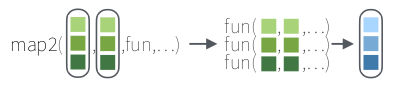
\includegraphics[width=4.01042in,height=\textheight]{Funcional/images/map2.png}

Vamos criar nossas listas para os próximos exemplos:

\textbf{Listas y, z e l2:}

\begin{Shaded}
\begin{Highlighting}[]
\NormalTok{y }\OtherTok{\textless{}{-}} \FunctionTok{list}\NormalTok{(}\DecValTok{1}\NormalTok{, }\DecValTok{2}\NormalTok{, }\DecValTok{3}\NormalTok{) }
\NormalTok{z }\OtherTok{\textless{}{-}} \FunctionTok{list}\NormalTok{(}\DecValTok{4}\NormalTok{, }\DecValTok{5}\NormalTok{, }\DecValTok{6}\NormalTok{)}
\NormalTok{l2 }\OtherTok{\textless{}{-}} \FunctionTok{list}\NormalTok{(}\AttributeTok{x =} \StringTok{"a"}\NormalTok{, }\AttributeTok{y =} \StringTok{"z"}\NormalTok{)}
\end{Highlighting}
\end{Shaded}

\hypertarget{map2}{%
\subsubsection{map2}\label{map2}}

Use para aplicar uma função em um \textbf{par de listas e retornar uma
lista}.

\begin{Shaded}
\begin{Highlighting}[]
\FunctionTok{map2}\NormalTok{(x,y,rep)}
\end{Highlighting}
\end{Shaded}

\begin{verbatim}
[[1]]
 [1]  1  2  3  4  5  6  7  8  9 10

[[2]]
 [1] 11 12 13 14 15 16 17 18 19 20 11 12 13 14 15 16 17 18 19 20

[[3]]
 [1] 21 22 23 24 25 26 27 28 29 30 21 22 23 24 25 26 27 28 29 30 21 22 23 24 25
[26] 26 27 28 29 30
\end{verbatim}

Veja que neste exemplo, para cada elemento da lista ``x'', aplicamos a
função rep() para replicar em número de vezes cada elemento da lista
``y''.

O purr possui uma sintaxe, onde ao invés de termos explicitamente o nome
de uma função, podemos criá-la no momento do mapeamento. Para maiores
detalhes veja \protect\hyperlink{atalhos-para-funuxe7uxf5es}{Atalhos
para funções}.

\begin{Shaded}
\begin{Highlighting}[]
\FunctionTok{map2}\NormalTok{(x,y, }\SpecialCharTok{\textasciitilde{}}\NormalTok{ .x}\SpecialCharTok{*}\NormalTok{.y)}
\end{Highlighting}
\end{Shaded}

\begin{verbatim}
[[1]]
 [1]  1  2  3  4  5  6  7  8  9 10

[[2]]
 [1] 22 24 26 28 30 32 34 36 38 40

[[3]]
 [1] 63 66 69 72 75 78 81 84 87 90
\end{verbatim}

Ao invés de usarmos uma função que multiplicasse dois números,
simplesmente declaramos uma função com o ``\textasciitilde{}'' e depois
informamos o que esta função fará, neste caso, irá multiplicar ``*'' os
elementos da lista ``x'' pelos da lista ``y''.

\hypertarget{map2_dbl}{%
\subsubsection{map2\_dbl}\label{map2_dbl}}

Use para aplicar uma função em um \textbf{par de listas e retornar um
vetor double}.

\begin{Shaded}
\begin{Highlighting}[]
\FunctionTok{map2\_dbl}\NormalTok{(y, z, }\SpecialCharTok{\textasciitilde{}}\NormalTok{ .x }\SpecialCharTok{/}\NormalTok{ .y)}
\end{Highlighting}
\end{Shaded}

\begin{verbatim}
[1] 0.25 0.40 0.50
\end{verbatim}

\hypertarget{map2_int}{%
\subsubsection{map2\_int}\label{map2_int}}

Use para aplicar uma função em um \textbf{par de listas e retornar um
vetor de inteiros}.

\begin{Shaded}
\begin{Highlighting}[]
\FunctionTok{map2\_int}\NormalTok{(}\FunctionTok{as.integer}\NormalTok{(y), }\FunctionTok{as.integer}\NormalTok{(z), }\StringTok{\textasciigrave{}}\AttributeTok{+}\StringTok{\textasciigrave{}}\NormalTok{)}
\end{Highlighting}
\end{Shaded}

\begin{verbatim}
[1] 5 7 9
\end{verbatim}

\hypertarget{map2_chr}{%
\subsubsection{map2\_chr}\label{map2_chr}}

Use para aplicar uma função em um \textbf{par de listas e retornar um
vetor de caracteres}.

\begin{Shaded}
\begin{Highlighting}[]
\FunctionTok{map2\_chr}\NormalTok{(l1, l2, paste, }\AttributeTok{collapse =} \StringTok{","}\NormalTok{, }\AttributeTok{sep =} \StringTok{":"}\NormalTok{)}
\end{Highlighting}
\end{Shaded}

\begin{verbatim}
        x         y 
"a:a,b:a" "c:z,d:z" 
\end{verbatim}

\hypertarget{map2_lgl}{%
\subsubsection{map2\_lgl}\label{map2_lgl}}

Use para aplicar uma função em um \textbf{par de listas e retornar um
vetor lógico}.

\begin{Shaded}
\begin{Highlighting}[]
\FunctionTok{map2\_lgl}\NormalTok{(l2, l1, }\StringTok{\textasciigrave{}}\AttributeTok{\%in\%}\StringTok{\textasciigrave{}}\NormalTok{)}
\end{Highlighting}
\end{Shaded}

\begin{verbatim}
    x     y 
 TRUE FALSE 
\end{verbatim}

\hypertarget{map2_dfc}{%
\subsubsection{map2\_dfc}\label{map2_dfc}}

Use para aplicar uma função em um \textbf{par de listas e retornar um
data frame agrupado por colunas}.

\begin{Shaded}
\begin{Highlighting}[]
\FunctionTok{map2\_dfc}\NormalTok{(l1, l2,}\SpecialCharTok{\textasciitilde{}} \FunctionTok{as.data.frame}\NormalTok{(}\FunctionTok{c}\NormalTok{(.x, .y)))}
\end{Highlighting}
\end{Shaded}

\begin{verbatim}
  c(.x, .y)...1 c(.x, .y)...2
1             a             c
2             b             d
3             a             z
\end{verbatim}

\hypertarget{map2_dfr}{%
\subsubsection{map2\_dfr}\label{map2_dfr}}

Use para aplicar uma função em um \textbf{par de listas e retornar um
data frame agrupado por linhas}.

\begin{Shaded}
\begin{Highlighting}[]
\FunctionTok{map2\_dfr}\NormalTok{(l1, l2,}\SpecialCharTok{\textasciitilde{}} \FunctionTok{as.data.frame}\NormalTok{(}\FunctionTok{c}\NormalTok{(.x, .y)))}
\end{Highlighting}
\end{Shaded}

\begin{verbatim}
  c(.x, .y)
1         a
2         b
3         a
4         c
5         d
6         z
\end{verbatim}

\hypertarget{walk2}{%
\subsubsection{walk2}\label{walk2}}

Use esta para executar uma atividade assim como a função map2(), mas de
forma \textbf{silenciosa}, ou seja, se houver mensagens de saída, elas
não aparecerão. Ela também retorna a primeira lista de \textbf{entrada}.
Isto ajuda em situações com o pipe ou por exemplo, quando precisamos
salvar multiplos arquivos mas não queremos as mensagens de saída em
nosso processo.

\begin{Shaded}
\begin{Highlighting}[]
\FunctionTok{walk2}\NormalTok{(l1,l2, }\SpecialCharTok{\textasciitilde{}}\FunctionTok{c}\NormalTok{(.x,.y))}
\end{Highlighting}
\end{Shaded}

\hypertarget{vuxe1rias-listas}{%
\subsection{Várias listas}\label{vuxe1rias-listas}}

O pacote purr tem um conjunto de funções similares ao map(), porém, ao
invés de receber apenas uma única lista de entrada e retornar um vetor
de mesmo tamanho, elas \textbf{aceitam uma lista com outras listas ou
vetores (com um data frame)} e \textbf{retornam também um vetor de mesmo
tamanho na saída}.

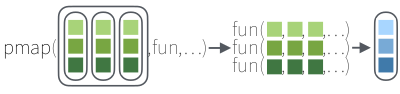
\includegraphics[width=4.04167in,height=\textheight]{Funcional/images/pmap.png}

Vejamos as princpais funções deste tipo:

\hypertarget{pmap}{%
\subsubsection{pmap}\label{pmap}}

Diagmos que temos três listas (x,y e z) e precisamos aplicar uma função
à elas. Neste caso,

\begin{Shaded}
\begin{Highlighting}[]
\FunctionTok{pmap}\NormalTok{(}\FunctionTok{list}\NormalTok{(x,y,z), sum)}
\end{Highlighting}
\end{Shaded}

\begin{verbatim}
[[1]]
[1] 60

[[2]]
[1] 162

[[3]]
[1] 264
\end{verbatim}

Assim como explicado com as funções map() e map2(), temos as variantes
abaixo seguindo a mesma nomenclatura para pmap, sendo que cada uma delas
retornam os respectivo tipo após o \_ . Por exemplo, a pmap\_dbl()
funciona similar ao pmap(), porém retorna uma lista de vetores double e
assim por diante.

\begin{itemize}
\item
  \textbf{pmap\_dbl}
\item
  \textbf{pmap\_int}
\item
  \textbf{pmap\_chr}
\item
  \textbf{pmap\_lgl}
\item
  \textbf{pmap\_dfc}
\item
  \textbf{pmap\_dfr}
\item
  \textbf{pwalk}
\end{itemize}

\hypertarget{listas-e-uxedndices}{%
\subsection{Listas e índices}\label{listas-e-uxedndices}}

O pacote purr tem um conjunto de funções similares ao map(), porém, ao
invés de receber apenas uma única lista de entrada e retornar um vetor
de mesmo tamanho, elas \textbf{aplicam uma função para cada elemento e
seu índice}.

Usamos o símbolo \textasciitilde{} para declarar uma fórmula, .x para
acessar os valores dos elementos e .y para acessar o índice do elemento.

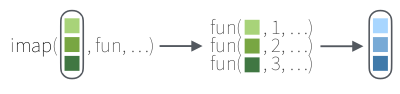
\includegraphics[width=3.96875in,height=\textheight]{Funcional/images/imap.png}

\hypertarget{imap}{%
\subsubsection{imap}\label{imap}}

\begin{Shaded}
\begin{Highlighting}[]
\FunctionTok{imap}\NormalTok{(y, }\SpecialCharTok{\textasciitilde{}}\FunctionTok{paste0}\NormalTok{(.y, }\StringTok{": "}\NormalTok{, .x))}
\end{Highlighting}
\end{Shaded}

\begin{verbatim}
[[1]]
[1] "1: 1"

[[2]]
[1] "2: 2"

[[3]]
[1] "3: 3"
\end{verbatim}

Assim como explicado com as funções map() e map2(), temos as variantes
abaixo seguindo a mesma nomenclatura para imap, sendo que cada uma delas
retornam os respectivos tipo após o \_ .

Por exemplo, a imap\_dbl() funciona similar ao imap(), porém retorna uma
lista de vetores double e assim por diante.

\begin{itemize}
\item
  \textbf{imap\_dbl}
\item
  \textbf{imap\_int}
\item
  \textbf{imap\_chr}
\item
  \textbf{imap\_lgl}
\item
  \textbf{imap\_dfc}
\item
  \textbf{imap\_dfr}
\item
  \textbf{iwalk}
\end{itemize}

\hypertarget{atalhos-para-funuxe7uxf5es}{%
\section{Atalhos para funções}\label{atalhos-para-funuxe7uxf5es}}

Até o momento, na maioria dos casos, declaramos o nome da função durante
o processo de mapeamento, mas o pacote purr possui alguns atalhos para
faciliar este processo. Também não mencionamos, mas as funções vistas
até aqui, não aceitam apenas \textbf{funções}, mas também
\textbf{fórmulas} ou \textbf{vetores}.

Temos atalhos de funções para cenários de uma, duas, várias e listas e
índices.

\begin{itemize}
\tightlist
\item
  Atalho para \textbf{Uma Lista}, por exemplo, usando map() ou suas
  derivações:
\end{itemize}

Use \textbf{\textasciitilde.} para passar um argumento para a função:

\begin{Shaded}
\begin{Highlighting}[]
    \FunctionTok{map}\NormalTok{(y, }\SpecialCharTok{\textasciitilde{}}\NormalTok{.}\SpecialCharTok{+}\DecValTok{2}\NormalTok{)}
\end{Highlighting}
\end{Shaded}

\begin{verbatim}
[[1]]
[1] 3

[[2]]
[1] 4

[[3]]
[1] 5
\end{verbatim}

O atalho acima, é o mesmo que declararmos uma função x por exemplo:

\begin{Shaded}
\begin{Highlighting}[]
    \FunctionTok{map}\NormalTok{(y,}\ControlFlowTok{function}\NormalTok{(x) x}\SpecialCharTok{+}\DecValTok{2}\NormalTok{)}
\end{Highlighting}
\end{Shaded}

\begin{verbatim}
[[1]]
[1] 3

[[2]]
[1] 4

[[3]]
[1] 5
\end{verbatim}

Apenas para ilustrar as possibildades, digamos que precisemos encurtar
os nomes dos filmes de starwars que cada personagem participou. Para
isto podemos fazer algo como:

\begin{Shaded}
\begin{Highlighting}[]
\NormalTok{sw\_trunc }\OtherTok{\textless{}{-}} 
  \FunctionTok{map}\NormalTok{(starwars}\SpecialCharTok{$}\NormalTok{films, }\SpecialCharTok{\textasciitilde{}}\FunctionTok{str\_trunc}\NormalTok{(., }\AttributeTok{width=}\DecValTok{15}\NormalTok{, }\AttributeTok{side=}\StringTok{"right"}\NormalTok{)) }\SpecialCharTok{|\textgreater{}} 
  \FunctionTok{set\_names}\NormalTok{(starwars}\SpecialCharTok{$}\NormalTok{name) }
\NormalTok{sw\_trunc[}\DecValTok{1}\SpecialCharTok{:}\DecValTok{3}\NormalTok{]}
\end{Highlighting}
\end{Shaded}

\begin{verbatim}
$`Luke Skywalker`
[1] "The Empire S..." "Revenge of t..." "Return of th..." "A New Hope"     
[5] "The Force Aw..."

$`C-3PO`
[1] "The Empire S..." "Attack of th..." "The Phantom ..." "Revenge of t..."
[5] "Return of th..." "A New Hope"     

$`R2-D2`
[1] "The Empire S..." "Attack of th..." "The Phantom ..." "Revenge of t..."
[5] "Return of th..." "A New Hope"      "The Force Aw..."
\end{verbatim}

\begin{itemize}
\tightlist
\item
  Atalho para \textbf{Duas Listas}, por exemplo, usando map2() ou suas
  derivações:
\end{itemize}

Use \textasciitilde.x.y para passar dois argumentos:

\begin{Shaded}
\begin{Highlighting}[]
    \FunctionTok{map2}\NormalTok{(y,z,}\SpecialCharTok{\textasciitilde{}}\NormalTok{.x}\SpecialCharTok{+}\NormalTok{.y)}
\end{Highlighting}
\end{Shaded}

\begin{verbatim}
[[1]]
[1] 5

[[2]]
[1] 7

[[3]]
[1] 9
\end{verbatim}

O atalho acima, seria o mesmo que declararmos uma função passando dois
argumentos como:

\begin{Shaded}
\begin{Highlighting}[]
    \FunctionTok{map2}\NormalTok{(y,z,}\ControlFlowTok{function}\NormalTok{(a,b) a}\SpecialCharTok{+}\NormalTok{b)}
\end{Highlighting}
\end{Shaded}

\begin{verbatim}
[[1]]
[1] 5

[[2]]
[1] 7

[[3]]
[1] 9
\end{verbatim}

\begin{itemize}
\tightlist
\item
  Atalho para \textbf{Várias Listas}, por exemplo, usando pmap() ou suas
  derivações:
\end{itemize}

Use \textasciitilde..1 ..2 ..3 etc para passar multiplos argumentos para
a função sem declará-la:

\begin{Shaded}
\begin{Highlighting}[]
    \FunctionTok{pmap}\NormalTok{(}\FunctionTok{list}\NormalTok{(x,y,z), }\SpecialCharTok{\textasciitilde{}}\NormalTok{..}\DecValTok{3} \SpecialCharTok{+}\NormalTok{ ..}\DecValTok{1} \SpecialCharTok{{-}}\NormalTok{ ..}\DecValTok{2}\NormalTok{)}
\end{Highlighting}
\end{Shaded}

\begin{verbatim}
[[1]]
 [1]  4  5  6  7  8  9 10 11 12 13

[[2]]
 [1] 14 15 16 17 18 19 20 21 22 23

[[3]]
 [1] 24 25 26 27 28 29 30 31 32 33
\end{verbatim}

O atalho acima, seria o mesmo que declararmos uma função com três
argumentos

\begin{Shaded}
\begin{Highlighting}[]
    \FunctionTok{pmap}\NormalTok{(}\FunctionTok{list}\NormalTok{(x,y,z), }\ControlFlowTok{function}\NormalTok{(a,b,c) c}\SpecialCharTok{+}\NormalTok{a}\SpecialCharTok{{-}}\NormalTok{b)}
\end{Highlighting}
\end{Shaded}

\begin{verbatim}
[[1]]
 [1]  4  5  6  7  8  9 10 11 12 13

[[2]]
 [1] 14 15 16 17 18 19 20 21 22 23

[[3]]
 [1] 24 25 26 27 28 29 30 31 32 33
\end{verbatim}

\begin{itemize}
\tightlist
\item
  Atalho para \textbf{Listas e Índices}, por exemplo, usando imap() ou
  suas derivações:
\end{itemize}

Use \textasciitilde{} .x .y , sendo que .x retorna o valor da lista e .y
o valor do índice.

\begin{Shaded}
\begin{Highlighting}[]
    \FunctionTok{imap}\NormalTok{(}\FunctionTok{list}\NormalTok{(x, y, z), }\SpecialCharTok{\textasciitilde{}}\FunctionTok{paste0}\NormalTok{(.y, }\StringTok{": "}\NormalTok{, .x))}
\end{Highlighting}
\end{Shaded}

\begin{verbatim}
[[1]]
[1] "1: 1:10"  "1: 11:20" "1: 21:30"

[[2]]
[1] "2: 1" "2: 2" "2: 3"

[[3]]
[1] "3: 4" "3: 5" "3: 6"
\end{verbatim}

O atalho acima, retornou
\textless índice\textgreater:\textless valor\textgreater{}

\hypertarget{acessando-os-elementos}{%
\section{Acessando os elementos}\label{acessando-os-elementos}}

Podemos usar uma string ou um inteiro com qualquer função map para
indexar elementos das listas por nome ou posição.

Vejamos um exemplo. Para obter o \textbf{segundo} valor de cada elemento
na lista ``l1'', podemos usar

\begin{Shaded}
\begin{Highlighting}[]
    \FunctionTok{map}\NormalTok{(l1, }\DecValTok{2}\NormalTok{)}
\end{Highlighting}
\end{Shaded}

\begin{verbatim}
$x
[1] "b"

$y
[1] "d"
\end{verbatim}

O código acima, seria o mesmo que escrever:

\begin{Shaded}
\begin{Highlighting}[]
    \FunctionTok{map}\NormalTok{(l1, }\ControlFlowTok{function}\NormalTok{(x)x[[}\DecValTok{2}\NormalTok{]])}
\end{Highlighting}
\end{Shaded}

\begin{verbatim}
$x
[1] "b"

$y
[1] "d"
\end{verbatim}

\hypertarget{trabalhando-com-listas}{%
\section{Trabalhando com Listas}\label{trabalhando-com-listas}}

Como vimos na função map(), map2(), pmap(), imap(), a estrutura de lista
é essencial, pois é a entrada e saída destas funções, por isso, o pacote
purr possui diversas funções que permitem manipular listas, com filtrar,
remodelar, combinar, modificar e reduzí-las. Veremos a seguir diversas
destas funções.

\hypertarget{filtros}{%
\subsection{Filtros}\label{filtros}}

\hypertarget{keep}{%
\subsubsection{keep}\label{keep}}

Use para manter os elementos que passam em um teste lógico. Por exemplo,
em nossa lista ``x'', temos 3 elementos.

\begin{Shaded}
\begin{Highlighting}[]
\NormalTok{x}
\end{Highlighting}
\end{Shaded}

\begin{verbatim}
[[1]]
 [1]  1  2  3  4  5  6  7  8  9 10

[[2]]
 [1] 11 12 13 14 15 16 17 18 19 20

[[3]]
 [1] 21 22 23 24 25 26 27 28 29 30
\end{verbatim}

Digamos que precisamos manter na lista, apenas os vetores que tem a o
valor máximo maior que 15. Para isso, podemos fazer:

\begin{Shaded}
\begin{Highlighting}[]
\FunctionTok{keep}\NormalTok{ (x, }\ControlFlowTok{function}\NormalTok{(x) }\FunctionTok{max}\NormalTok{(x)}\SpecialCharTok{\textgreater{}}\DecValTok{15}\NormalTok{)}
\end{Highlighting}
\end{Shaded}

\begin{verbatim}
[[1]]
 [1] 11 12 13 14 15 16 17 18 19 20

[[2]]
 [1] 21 22 23 24 25 26 27 28 29 30
\end{verbatim}

Veja que apenas os dois últimos elementos de ``x'' passaram pelo teste
(max \textgreater15) e por isso, foram retornados pela função.

Se quiser fazer o oposto, ou seja, ao invés de retornar os items que
passaram pelo teste, manter os que não passaram, podemos usar a função
discard().

\begin{Shaded}
\begin{Highlighting}[]
\FunctionTok{discard}\NormalTok{ (x, }\ControlFlowTok{function}\NormalTok{(x) }\FunctionTok{max}\NormalTok{(x)}\SpecialCharTok{\textgreater{}}\DecValTok{15}\NormalTok{)}
\end{Highlighting}
\end{Shaded}

\begin{verbatim}
[[1]]
 [1]  1  2  3  4  5  6  7  8  9 10
\end{verbatim}

Se usarmos o atalho para função como visto anteriormente, poderíamos
reescrever o código anteior como:

\begin{Shaded}
\begin{Highlighting}[]
\FunctionTok{discard}\NormalTok{ (x, }\SpecialCharTok{\textasciitilde{}}\FunctionTok{max}\NormalTok{(.)}\SpecialCharTok{\textgreater{}}\DecValTok{15}\NormalTok{)}
\end{Highlighting}
\end{Shaded}

\begin{verbatim}
[[1]]
 [1]  1  2  3  4  5  6  7  8  9 10
\end{verbatim}

\hypertarget{compact}{%
\subsubsection{compact}\label{compact}}

Use para excluir elementos em branco. Por exemplo, digamos que temos uma
lista ``x\_na'' que possui 7 elementos, sendo que quarto é nulo:

\begin{Shaded}
\begin{Highlighting}[]
\NormalTok{x\_nulo }\OtherTok{\textless{}{-}} \FunctionTok{splice}\NormalTok{(x, }\ConstantTok{NULL}\NormalTok{, y)}
\NormalTok{x\_nulo}
\end{Highlighting}
\end{Shaded}

\begin{verbatim}
[[1]]
 [1]  1  2  3  4  5  6  7  8  9 10

[[2]]
 [1] 11 12 13 14 15 16 17 18 19 20

[[3]]
 [1] 21 22 23 24 25 26 27 28 29 30

[[4]]
NULL

[[5]]
[1] 1

[[6]]
[1] 2

[[7]]
[1] 3
\end{verbatim}

Usando a função compact() iremos remover os elementos ausentes:

\begin{Shaded}
\begin{Highlighting}[]
\FunctionTok{compact}\NormalTok{(x\_nulo)}
\end{Highlighting}
\end{Shaded}

\begin{verbatim}
[[1]]
 [1]  1  2  3  4  5  6  7  8  9 10

[[2]]
 [1] 11 12 13 14 15 16 17 18 19 20

[[3]]
 [1] 21 22 23 24 25 26 27 28 29 30

[[4]]
[1] 1

[[5]]
[1] 2

[[6]]
[1] 3
\end{verbatim}

\hypertarget{head_while}{%
\subsubsection{head\_while}\label{head_while}}

Use para retornar os elementos do topo da lista, até encontrar o
primeiro que não passa no teste lógico. No exemplo a seguir, iremos
obter os valores do topo da lista até que um valor não passe no teste
lógico, neste caso, não passe no teste de não ser numérico. Portanto, ao
encontrar o elemento nulo, ele irá passar e retornar os elementos do
topo encontrados até o momento.

\begin{Shaded}
\begin{Highlighting}[]
\FunctionTok{head\_while}\NormalTok{(x\_nulo, }\ControlFlowTok{function}\NormalTok{ (x) }\FunctionTok{is.numeric}\NormalTok{(x))}
\end{Highlighting}
\end{Shaded}

\begin{verbatim}
[[1]]
 [1]  1  2  3  4  5  6  7  8  9 10

[[2]]
 [1] 11 12 13 14 15 16 17 18 19 20

[[3]]
 [1] 21 22 23 24 25 26 27 28 29 30
\end{verbatim}

Para fazer o mesmo processo, porém pegar os elementos do fim da lista,
ao invés do topo use a função tail\_while(). Por exemplo, quando
precisamos obter os elementos do fim da lista, até encontrarmos um valor
que não tenho mais que 1 caractere.

\begin{Shaded}
\begin{Highlighting}[]
\FunctionTok{tail\_while}\NormalTok{(x\_nulo, }\SpecialCharTok{\textasciitilde{}}\FunctionTok{length}\NormalTok{(.}\SpecialCharTok{\textless{}}\DecValTok{2}\NormalTok{))}
\end{Highlighting}
\end{Shaded}

\begin{verbatim}
[[1]]
[1] 1

[[2]]
[1] 2

[[3]]
[1] 3
\end{verbatim}

\hypertarget{detect}{%
\subsubsection{detect}\label{detect}}

Use para encontrar o primeiro elemento que passa no teste lógico. Usamos
os argumentos ``\textbf{dir=}'' para definir se queremos buscar do
início da lista até o fim (\textbf{forward}) (padrão) ou o inverso
(\textbf{backward}). No exemplo a seguir, iremos encontrar o elemento
que tem o valor máximo menor que 15, mas varrendo a lista de baixo para
cima:

\begin{Shaded}
\begin{Highlighting}[]
\FunctionTok{detect}\NormalTok{ (x\_nulo, }\SpecialCharTok{\textasciitilde{}}\FunctionTok{max}\NormalTok{(.)}\SpecialCharTok{\textless{}}\DecValTok{15}\NormalTok{, }\AttributeTok{dir=}\StringTok{"backward"}\NormalTok{)}
\end{Highlighting}
\end{Shaded}

\begin{verbatim}
 [1]  1  2  3  4  5  6  7  8  9 10
\end{verbatim}

\begin{tcolorbox}[enhanced jigsaw, rightrule=.15mm, arc=.35mm, coltitle=black, colframe=quarto-callout-tip-color-frame, opacityback=0, toprule=.15mm, left=2mm, breakable, colback=white, bottomtitle=1mm, leftrule=.75mm, title=\textcolor{quarto-callout-tip-color}{\faLightbulb}\hspace{0.5em}{Dica}, colbacktitle=quarto-callout-tip-color!10!white, titlerule=0mm, bottomrule=.15mm, toptitle=1mm, opacitybacktitle=0.6]
Se quisermos obter o índice do elemento ao invés dos valores do
elemento, podemos usar a função \textbf{detect\_index}()
\end{tcolorbox}

\begin{Shaded}
\begin{Highlighting}[]
\FunctionTok{detect\_index}\NormalTok{(x\_nulo, }\SpecialCharTok{\textasciitilde{}}\FunctionTok{max}\NormalTok{(.)}\SpecialCharTok{\textless{}}\DecValTok{15}\NormalTok{)}
\end{Highlighting}
\end{Shaded}

\begin{verbatim}
[1] 1
\end{verbatim}

\hypertarget{every}{%
\subsubsection{every}\label{every}}

Use para verificar se \textbf{todos os elementos} da lista passam no
teste lógico.

\begin{Shaded}
\begin{Highlighting}[]
\FunctionTok{every}\NormalTok{(x\_nulo, }\SpecialCharTok{\textasciitilde{}}\FunctionTok{max}\NormalTok{(.)}\SpecialCharTok{\textless{}}\DecValTok{15}\NormalTok{)}
\end{Highlighting}
\end{Shaded}

\begin{verbatim}
[1] FALSE
\end{verbatim}

\hypertarget{some}{%
\subsubsection{some}\label{some}}

Use para verificar se \textbf{algum elemento} da lista passam no teste
lógico.

\begin{Shaded}
\begin{Highlighting}[]
\FunctionTok{some}\NormalTok{(x\_nulo, }\SpecialCharTok{\textasciitilde{}}\FunctionTok{max}\NormalTok{(.)}\SpecialCharTok{\textless{}}\DecValTok{15}\NormalTok{)}
\end{Highlighting}
\end{Shaded}

\begin{verbatim}
[1] TRUE
\end{verbatim}

\hypertarget{none}{%
\subsubsection{none}\label{none}}

Use para verificar se \textbf{nenhum elemento} da lista passam no teste
lógico.

\begin{Shaded}
\begin{Highlighting}[]
\FunctionTok{none}\NormalTok{(x\_nulo, }\SpecialCharTok{\textasciitilde{}}\FunctionTok{max}\NormalTok{(.)}\SpecialCharTok{\textless{}}\DecValTok{15}\NormalTok{)}
\end{Highlighting}
\end{Shaded}

\begin{verbatim}
[1] FALSE
\end{verbatim}

\hypertarget{has_element}{%
\subsubsection{has\_element}\label{has_element}}

Use para verificar se uma lista tem determinado elemento.

\begin{Shaded}
\begin{Highlighting}[]
\NormalTok{elemento }\OtherTok{\textless{}{-}} \DecValTok{2}
\FunctionTok{has\_element}\NormalTok{(x\_nulo, elemento)}
\end{Highlighting}
\end{Shaded}

\begin{verbatim}
[1] TRUE
\end{verbatim}

\hypertarget{vec_depth}{%
\subsubsection{vec\_depth}\label{vec_depth}}

Use para obter a profundidade (número de níveis dos índices) de uma
lista. Para exemplificar melhor, vamos criar uma lista com outras listas
dentro:

\begin{Shaded}
\begin{Highlighting}[]
\CommentTok{\#Criamos uma lista "lista\_profunda" que tem como primeiro elemento a lista "x" e como segundo elemento a lista "y".}

\NormalTok{lista\_profunda }\OtherTok{\textless{}{-}} \FunctionTok{list}\NormalTok{(x, y)}
\FunctionTok{vec\_depth}\NormalTok{(lista\_profunda)}
\end{Highlighting}
\end{Shaded}

\begin{verbatim}
[1] 3
\end{verbatim}

\begin{Shaded}
\begin{Highlighting}[]
\CommentTok{\# Se adicionarmos uma outra lista na lista "x", teremos um nível a mais:}

\NormalTok{x\_com\_sublista }\OtherTok{\textless{}{-}} \FunctionTok{append}\NormalTok{(x, }\FunctionTok{list}\NormalTok{(}\FunctionTok{list}\NormalTok{(}\DecValTok{1}\SpecialCharTok{:}\DecValTok{5}\NormalTok{)))}
\NormalTok{lista\_mais\_profunda }\OtherTok{\textless{}{-}} \FunctionTok{list}\NormalTok{(x\_com\_sublista, y)}
\FunctionTok{vec\_depth}\NormalTok{(lista\_mais\_profunda)}
\end{Highlighting}
\end{Shaded}

\begin{verbatim}
[1] 4
\end{verbatim}

\begin{tcolorbox}[enhanced jigsaw, rightrule=.15mm, arc=.35mm, coltitle=black, colframe=quarto-callout-note-color-frame, opacityback=0, toprule=.15mm, left=2mm, breakable, colback=white, bottomtitle=1mm, leftrule=.75mm, title=\textcolor{quarto-callout-note-color}{\faInfo}\hspace{0.5em}{Nota}, colbacktitle=quarto-callout-note-color!10!white, titlerule=0mm, bottomrule=.15mm, toptitle=1mm, opacitybacktitle=0.6]
Temos sempre nível + 1, pois ele conta o nível 0 que é da própria lista.
\end{tcolorbox}

\hypertarget{uxedndices}{%
\subsection{Índices}\label{uxedndices}}

O pacote purr tem uma série de funções para identificar elementos de uma
lista, definí-los e/ou alterá-los por este índice. Vejamos algumas:

\hypertarget{pluck}{%
\subsubsection{pluck}\label{pluck}}

Use para selecionar um elemento por nome ou índice.

\begin{Shaded}
\begin{Highlighting}[]
\FunctionTok{pluck}\NormalTok{(x, }\DecValTok{2}\NormalTok{)}
\end{Highlighting}
\end{Shaded}

\begin{verbatim}
 [1] 11 12 13 14 15 16 17 18 19 20
\end{verbatim}

Neste caso, usamos a função pluck para obter o elemento no índice 2.
Vamos agora dar nome aos elementos da lista ``x'', usando a função
\textbf{set\_names}() do purr e depois obter o memos elemento por nome:

\begin{Shaded}
\begin{Highlighting}[]
\NormalTok{x }\OtherTok{\textless{}{-}} \FunctionTok{set\_names}\NormalTok{(x, }\FunctionTok{c}\NormalTok{(}\StringTok{"a"}\NormalTok{, }\StringTok{"b"}\NormalTok{, }\StringTok{"c"}\NormalTok{))}
\FunctionTok{pluck}\NormalTok{(x, }\StringTok{"b"}\NormalTok{)}
\end{Highlighting}
\end{Shaded}

\begin{verbatim}
 [1] 11 12 13 14 15 16 17 18 19 20
\end{verbatim}

\hypertarget{assign_in}{%
\subsubsection{assign\_in}\label{assign_in}}

Use para definir um \textbf{valor ao elemento} de acordo como a seleção
feita na função \textbf{pluck}()

\begin{Shaded}
\begin{Highlighting}[]
\FunctionTok{assign\_in}\NormalTok{(x, }\StringTok{"b"}\NormalTok{, }\DecValTok{5}\NormalTok{)}
\end{Highlighting}
\end{Shaded}

\begin{verbatim}
$a
 [1]  1  2  3  4  5  6  7  8  9 10

$b
[1] 5

$c
 [1] 21 22 23 24 25 26 27 28 29 30
\end{verbatim}

\hypertarget{modify_in}{%
\subsubsection{modify\_in}\label{modify_in}}

Use para aplicar uma função de modificação nos valores do elemento
selecionado como na função \textbf{pluck}().

\begin{Shaded}
\begin{Highlighting}[]
\FunctionTok{modify\_in}\NormalTok{(x, }\StringTok{"b"}\NormalTok{, log)}
\end{Highlighting}
\end{Shaded}

\begin{verbatim}
$a
 [1]  1  2  3  4  5  6  7  8  9 10

$b
 [1] 2.397895 2.484907 2.564949 2.639057 2.708050 2.772589 2.833213 2.890372
 [9] 2.944439 2.995732

$c
 [1] 21 22 23 24 25 26 27 28 29 30
\end{verbatim}

\hypertarget{remodelagem}{%
\subsection{Remodelagem}\label{remodelagem}}

O pacote purr possui uma série de funções para remodelar a forma de uma
lista. Vejamos algumas delas:

\hypertarget{flatten}{%
\subsubsection{flatten}\label{flatten}}

Use para remover um nível de índice (profundidade) de uma lista. Ver
também a função \protect\hyperlink{vec_depth}{vec\_depth} para obter o
número de profundidade de uma lista.

\begin{Shaded}
\begin{Highlighting}[]
\FunctionTok{flatten}\NormalTok{ (lista\_profunda)}
\end{Highlighting}
\end{Shaded}

\begin{verbatim}
[[1]]
 [1]  1  2  3  4  5  6  7  8  9 10

[[2]]
 [1] 11 12 13 14 15 16 17 18 19 20

[[3]]
 [1] 21 22 23 24 25 26 27 28 29 30

[[4]]
[1] 1

[[5]]
[1] 2

[[6]]
[1] 3
\end{verbatim}

\hypertarget{array_tree}{%
\subsubsection{array\_tree}\label{array_tree}}

Use para transformar um array (estrutura de uma ou mais dimensão que
contém o mesmo tipo de dados) em uma lista. É útil para permitir ouso de
arrays em funções com as do purr, que aceitam listas.

\begin{Shaded}
\begin{Highlighting}[]
\NormalTok{meu\_array }\OtherTok{\textless{}{-}} \FunctionTok{array}\NormalTok{(}\DecValTok{1}\SpecialCharTok{:}\DecValTok{3}\NormalTok{, }\FunctionTok{c}\NormalTok{(}\DecValTok{2}\NormalTok{,}\DecValTok{4}\NormalTok{))}
\FunctionTok{array\_tree}\NormalTok{(meu\_array)}
\end{Highlighting}
\end{Shaded}

\begin{verbatim}
[[1]]
[[1]][[1]]
[1] 1

[[1]][[2]]
[1] 3

[[1]][[3]]
[1] 2

[[1]][[4]]
[1] 1


[[2]]
[[2]][[1]]
[1] 2

[[2]][[2]]
[1] 1

[[2]][[3]]
[1] 3

[[2]][[4]]
[1] 2
\end{verbatim}

\hypertarget{cross2}{%
\subsubsection{cross2}\label{cross2}}

Use para gerar as combinações possíveis entre os elementos duas listas.
Neste caso, iremos gerar um elemento de saída com o primeiro elemento de
x e o primeiro de y. Depois iremos ter o segundo elemento contendo o
primeiro elemento de x e segundo de y e assim por diante.

\begin{Shaded}
\begin{Highlighting}[]
\FunctionTok{cross2}\NormalTok{ (x,y)}
\end{Highlighting}
\end{Shaded}

\begin{verbatim}
[[1]]
[[1]][[1]]
 [1]  1  2  3  4  5  6  7  8  9 10

[[1]][[2]]
[1] 1


[[2]]
[[2]][[1]]
 [1] 11 12 13 14 15 16 17 18 19 20

[[2]][[2]]
[1] 1


[[3]]
[[3]][[1]]
 [1] 21 22 23 24 25 26 27 28 29 30

[[3]][[2]]
[1] 1


[[4]]
[[4]][[1]]
 [1]  1  2  3  4  5  6  7  8  9 10

[[4]][[2]]
[1] 2


[[5]]
[[5]][[1]]
 [1] 11 12 13 14 15 16 17 18 19 20

[[5]][[2]]
[1] 2


[[6]]
[[6]][[1]]
 [1] 21 22 23 24 25 26 27 28 29 30

[[6]][[2]]
[1] 2


[[7]]
[[7]][[1]]
 [1]  1  2  3  4  5  6  7  8  9 10

[[7]][[2]]
[1] 3


[[8]]
[[8]][[1]]
 [1] 11 12 13 14 15 16 17 18 19 20

[[8]][[2]]
[1] 3


[[9]]
[[9]][[1]]
 [1] 21 22 23 24 25 26 27 28 29 30

[[9]][[2]]
[1] 3
\end{verbatim}

\begin{tcolorbox}[enhanced jigsaw, rightrule=.15mm, arc=.35mm, coltitle=black, colframe=quarto-callout-tip-color-frame, opacityback=0, toprule=.15mm, left=2mm, breakable, colback=white, bottomtitle=1mm, leftrule=.75mm, title=\textcolor{quarto-callout-tip-color}{\faLightbulb}\hspace{0.5em}{Dica}, colbacktitle=quarto-callout-tip-color!10!white, titlerule=0mm, bottomrule=.15mm, toptitle=1mm, opacitybacktitle=0.6]
Para combinar três listas usando a função \textbf{cross3}(). Para mais
listas, usamos a função \textbf{cross\_df}().
\end{tcolorbox}

\hypertarget{transpose}{%
\subsubsection{transpose}\label{transpose}}

Use para transpor (mudar de linhas para colunas) a ordem dos índices em
uma lista muti-nível:

\begin{Shaded}
\begin{Highlighting}[]
\FunctionTok{transpose}\NormalTok{(lista\_profunda)}
\end{Highlighting}
\end{Shaded}

\begin{verbatim}
[[1]]
[[1]][[1]]
 [1]  1  2  3  4  5  6  7  8  9 10

[[1]][[2]]
[1] 1


[[2]]
[[2]][[1]]
 [1] 11 12 13 14 15 16 17 18 19 20

[[2]][[2]]
[1] 2


[[3]]
[[3]][[1]]
 [1] 21 22 23 24 25 26 27 28 29 30

[[3]][[2]]
[1] 3
\end{verbatim}

\hypertarget{set_names}{%
\subsubsection{set\_names}\label{set_names}}

Use para definir nomes de um vetor/lista diretamente ou atraveś de uma
função:

\begin{Shaded}
\begin{Highlighting}[]
\NormalTok{y }\OtherTok{\textless{}{-}} \FunctionTok{set\_names}\NormalTok{ (y, }\FunctionTok{c}\NormalTok{(}\StringTok{"a"}\NormalTok{, }\StringTok{"b"}\NormalTok{, }\StringTok{"c"}\NormalTok{))}
\NormalTok{y}
\end{Highlighting}
\end{Shaded}

\begin{verbatim}
$a
[1] 1

$b
[1] 2

$c
[1] 3
\end{verbatim}

\begin{Shaded}
\begin{Highlighting}[]
\FunctionTok{set\_names}\NormalTok{(y, letters[}\DecValTok{4}\SpecialCharTok{:}\DecValTok{6}\NormalTok{])}
\end{Highlighting}
\end{Shaded}

\begin{verbatim}
$d
[1] 1

$e
[1] 2

$f
[1] 3
\end{verbatim}

\begin{Shaded}
\begin{Highlighting}[]
\FunctionTok{set\_names}\NormalTok{(y, toupper)}
\end{Highlighting}
\end{Shaded}

\begin{verbatim}
$A
[1] 1

$B
[1] 2

$C
[1] 3
\end{verbatim}

\hypertarget{modificauxe7uxf5es}{%
\subsection{Modificações}\label{modificauxe7uxf5es}}

O pacote purr possui uma série de funções para modificar elementos de
uma lista. Vejamos algumas delas:

\hypertarget{modify}{%
\subsubsection{modify}\label{modify}}

Use para aplicar uma função à cada elemento de uma lista. Ela é similar
à função map(), porém, diferente do map() que retorna uma lista ou um
tipo específico quando utilizamos suas variantes (map\_dbl, map\_int,
etc), a função modify retorna sempre o tipo do bjeto recebido (uma lista
ou um vetor atômico).

Por exemplo, ao passar uma lista para a função, assim como a função
map(), elá irá aplicar uma função ou fórmula e retornará uma lista de
mesmo tamanho:

\begin{Shaded}
\begin{Highlighting}[]
\FunctionTok{modify}\NormalTok{(x, }\SpecialCharTok{\textasciitilde{}}\NormalTok{.}\SpecialCharTok{+}\DecValTok{2}\NormalTok{)}
\end{Highlighting}
\end{Shaded}

\begin{verbatim}
$a
 [1]  3  4  5  6  7  8  9 10 11 12

$b
 [1] 13 14 15 16 17 18 19 20 21 22

$c
 [1] 23 24 25 26 27 28 29 30 31 32
\end{verbatim}

Se passarmos um vetor de inteiros, ela aplicará uma função e retornará
um vetor de mesmo tamanho de inteiros:

\begin{Shaded}
\begin{Highlighting}[]
\FunctionTok{modify}\NormalTok{ (mtcars}\SpecialCharTok{$}\NormalTok{wt, }\SpecialCharTok{\textasciitilde{}}\NormalTok{.}\SpecialCharTok{{-}}\DecValTok{2}\NormalTok{)}
\end{Highlighting}
\end{Shaded}

\begin{verbatim}
 [1]  0.620  0.875  0.320  1.215  1.440  1.460  1.570  1.190  1.150  1.440
[11]  1.440  2.070  1.730  1.780  3.250  3.424  3.345  0.200 -0.385 -0.165
[21]  0.465  1.520  1.435  1.840  1.845 -0.065  0.140 -0.487  1.170  0.770
[31]  1.570  0.780
\end{verbatim}

\hypertarget{modify_at}{%
\subsubsection{modify\_at}\label{modify_at}}

Use para modificar um elemento definido por seu índice ou nome.

\begin{Shaded}
\begin{Highlighting}[]
\FunctionTok{modify\_at}\NormalTok{(x, }\StringTok{"b"}\NormalTok{, }\SpecialCharTok{\textasciitilde{}}\NormalTok{.}\SpecialCharTok{*{-}}\DecValTok{1}\NormalTok{)}
\end{Highlighting}
\end{Shaded}

\begin{verbatim}
$a
 [1]  1  2  3  4  5  6  7  8  9 10

$b
 [1] -11 -12 -13 -14 -15 -16 -17 -18 -19 -20

$c
 [1] 21 22 23 24 25 26 27 28 29 30
\end{verbatim}

\hypertarget{modify_if}{%
\subsubsection{modify\_if}\label{modify_if}}

Use para modificar o(s) elemento(s) que passam por um teste lógico.
Neste exemplo, iremos definir uma fórmula que testa se o valor máximo de
um elemento é maior que 15. Para todos os elementos que passarem neste
teste, iremos multiplicá-los por -1.

\begin{Shaded}
\begin{Highlighting}[]
\FunctionTok{modify\_if}\NormalTok{(x, }\SpecialCharTok{\textasciitilde{}}\FunctionTok{max}\NormalTok{(.)}\SpecialCharTok{\textgreater{}}\DecValTok{15}\NormalTok{, }\SpecialCharTok{\textasciitilde{}}\NormalTok{.}\SpecialCharTok{*{-}}\DecValTok{1}\NormalTok{)}
\end{Highlighting}
\end{Shaded}

\begin{verbatim}
$a
 [1]  1  2  3  4  5  6  7  8  9 10

$b
 [1] -11 -12 -13 -14 -15 -16 -17 -18 -19 -20

$c
 [1] -21 -22 -23 -24 -25 -26 -27 -28 -29 -30
\end{verbatim}

\hypertarget{modify_depth}{%
\subsubsection{modify\_depth}\label{modify_depth}}

Use para aplicar uma função a cada elemento de uma lista que está à uma
certa profundidade (certo nível). Em geral, utilizamos quando temos
listas aninhadas (com outras listas dentro).

No exemplo abaixo, iremos retornar o maior valor, mas somente do
terceiro nível da lista. Como temos apenas um elemento neste nível
(lista\_mais\_profunda{[}{[}1{]}{]}{[}{[}4{]}{]}), apenas este será
usado para obter o maior valor atraveś da função max().

\begin{Shaded}
\begin{Highlighting}[]
\FunctionTok{modify\_depth}\NormalTok{(lista\_mais\_profunda, }\DecValTok{3}\NormalTok{, }\SpecialCharTok{\textasciitilde{}}\FunctionTok{max}\NormalTok{(.))}
\end{Highlighting}
\end{Shaded}

\begin{verbatim}
[[1]]
[[1]][[1]]
 [1]  1  2  3  4  5  6  7  8  9 10

[[1]][[2]]
 [1] 11 12 13 14 15 16 17 18 19 20

[[1]][[3]]
 [1] 21 22 23 24 25 26 27 28 29 30

[[1]][[4]]
[[1]][[4]][[1]]
[1] 5



[[2]]
[[2]][[1]]
[1] 1

[[2]][[2]]
[1] 2

[[2]][[3]]
[1] 3
\end{verbatim}

\begin{tcolorbox}[enhanced jigsaw, rightrule=.15mm, arc=.35mm, coltitle=black, colframe=quarto-callout-note-color-frame, opacityback=0, toprule=.15mm, left=2mm, breakable, colback=white, bottomtitle=1mm, leftrule=.75mm, title=\textcolor{quarto-callout-note-color}{\faInfo}\hspace{0.5em}{Nota}, colbacktitle=quarto-callout-note-color!10!white, titlerule=0mm, bottomrule=.15mm, toptitle=1mm, opacitybacktitle=0.6]
A função map() tem variações como map\_at() e map\_if() que fazem o
mesmo que as modify\_at ou modify\_if, porém retornando lista.
\end{tcolorbox}

\hypertarget{combinauxe7uxf5es}{%
\subsection{Combinações}\label{combinauxe7uxf5es}}

O pacote purr possui uma série de funções para combinar elementos de
diversas listas. Vejamos algumas delas:

\hypertarget{append}{%
\subsubsection{append}\label{append}}

Use para adicionar valores ao final de uma lista.

\begin{Shaded}
\begin{Highlighting}[]
\FunctionTok{append}\NormalTok{ (x, }\FunctionTok{list}\NormalTok{(}\FunctionTok{seq}\NormalTok{(}\DecValTok{55}\SpecialCharTok{:}\DecValTok{60}\NormalTok{),}\DecValTok{66}\NormalTok{,}\FunctionTok{c}\NormalTok{(}\StringTok{"aaa"}\NormalTok{, }\StringTok{"zzz"}\NormalTok{)))}
\end{Highlighting}
\end{Shaded}

\begin{verbatim}
$a
 [1]  1  2  3  4  5  6  7  8  9 10

$b
 [1] 11 12 13 14 15 16 17 18 19 20

$c
 [1] 21 22 23 24 25 26 27 28 29 30

[[4]]
[1] 1 2 3 4 5 6

[[5]]
[1] 66

[[6]]
[1] "aaa" "zzz"
\end{verbatim}

\begin{tcolorbox}[enhanced jigsaw, rightrule=.15mm, arc=.35mm, coltitle=black, colframe=quarto-callout-tip-color-frame, opacityback=0, toprule=.15mm, left=2mm, breakable, colback=white, bottomtitle=1mm, leftrule=.75mm, title=\textcolor{quarto-callout-tip-color}{\faLightbulb}\hspace{0.5em}{Dica}, colbacktitle=quarto-callout-tip-color!10!white, titlerule=0mm, bottomrule=.15mm, toptitle=1mm, opacitybacktitle=0.6]
Use o argumento \textbf{after=} para especificar o índice a partir de
onde os valores serão adicionados.
\end{tcolorbox}

\hypertarget{prepend}{%
\subsubsection{prepend}\label{prepend}}

Use para adicionar valores ao começo da lista.

\begin{Shaded}
\begin{Highlighting}[]
\FunctionTok{prepend}\NormalTok{(x , }\FunctionTok{list}\NormalTok{(}\AttributeTok{d =} \DecValTok{1}\NormalTok{))}
\end{Highlighting}
\end{Shaded}

\begin{verbatim}
$d
[1] 1

$a
 [1]  1  2  3  4  5  6  7  8  9 10

$b
 [1] 11 12 13 14 15 16 17 18 19 20

$c
 [1] 21 22 23 24 25 26 27 28 29 30
\end{verbatim}

\begin{tcolorbox}[enhanced jigsaw, rightrule=.15mm, arc=.35mm, coltitle=black, colframe=quarto-callout-tip-color-frame, opacityback=0, toprule=.15mm, left=2mm, breakable, colback=white, bottomtitle=1mm, leftrule=.75mm, title=\textcolor{quarto-callout-tip-color}{\faLightbulb}\hspace{0.5em}{Dica}, colbacktitle=quarto-callout-tip-color!10!white, titlerule=0mm, bottomrule=.15mm, toptitle=1mm, opacitybacktitle=0.6]
Use o argumento \textbf{before=} para determinar o índice ao qual iremos
adicionar os valores antes.
\end{tcolorbox}

\hypertarget{splice}{%
\subsubsection{splice}\label{splice}}

Use para combinar objetos em uma lista única.

\begin{Shaded}
\begin{Highlighting}[]
\FunctionTok{splice}\NormalTok{ (x, }\StringTok{"nova"}\NormalTok{, }\FunctionTok{c}\NormalTok{(}\StringTok{"a"}\NormalTok{, }\StringTok{"b"}\NormalTok{), }\FunctionTok{list}\NormalTok{(}\FunctionTok{seq}\NormalTok{(}\DecValTok{100}\SpecialCharTok{:}\DecValTok{110}\NormalTok{)))}
\end{Highlighting}
\end{Shaded}

\begin{verbatim}
$a
 [1]  1  2  3  4  5  6  7  8  9 10

$b
 [1] 11 12 13 14 15 16 17 18 19 20

$c
 [1] 21 22 23 24 25 26 27 28 29 30

[[4]]
[1] "nova"

[[5]]
[1] "a" "b"

[[6]]
 [1]  1  2  3  4  5  6  7  8  9 10 11
\end{verbatim}

\hypertarget{reduuxe7uxf5es}{%
\subsection{Reduções}\label{reduuxe7uxf5es}}

O pacote purr tem uma algumas funções para reduzir uma lista aplicado
funções de forma recursivas. Vejamos algumas:

\hypertarget{reduce}{%
\subsubsection{reduce}\label{reduce}}

Use para reduzir uma lista em um único valor, aplicando uma função
binária. Uma função binária, recebe dois valores e retorna apenas um
valor.

Por exemplo, utilziando nossa lista ``x'', iremos reduzí-la a um única
valor, pegando o valor do primeiro e segundo elementos, pegando seu
retorno, aplicando a mesma função com este resultado e o terceiro
elemento, e assim por diante;

\begin{Shaded}
\begin{Highlighting}[]
\CommentTok{\# func(a,b) {-}{-} res1 {-}{-}\textgreater{} func(res1, c) {-}{-} res\_final}
\NormalTok{x}
\end{Highlighting}
\end{Shaded}

\begin{verbatim}
$a
 [1]  1  2  3  4  5  6  7  8  9 10

$b
 [1] 11 12 13 14 15 16 17 18 19 20

$c
 [1] 21 22 23 24 25 26 27 28 29 30
\end{verbatim}

\begin{Shaded}
\begin{Highlighting}[]
\FunctionTok{reduce}\NormalTok{ (x, sum)}
\end{Highlighting}
\end{Shaded}

\begin{verbatim}
[1] 465
\end{verbatim}

\hypertarget{reduce2}{%
\subsubsection{reduce2}\label{reduce2}}

Use para reduzir uma lista em um único valor, aplicando uma função
ternária, ou seja, receber duas listas ou vertores e aplica uma função
que recebe três argumentos de forma recursiva.

Para este exemplo iremos criar uma função ternãria chamada paste2. Esta
função simplesmente recebe três argumentos, concatena usando a função
paste e retorna uma valor.

\begin{Shaded}
\begin{Highlighting}[]
\NormalTok{paste2 }\OtherTok{\textless{}{-}} \ControlFlowTok{function}\NormalTok{(x, y, }\AttributeTok{sep =} \StringTok{"."}\NormalTok{) }\FunctionTok{paste}\NormalTok{(x, y, }\AttributeTok{sep =}\NormalTok{ sep)}
\end{Highlighting}
\end{Shaded}

Através da função reduce2, podemos aplicar nossa função \textbf{paste2}
e fazermos sua aplicação de forma recursiva através das duas listas de
entrada ``x'' e ``y''.

\begin{tcolorbox}[enhanced jigsaw, rightrule=.15mm, arc=.35mm, coltitle=black, colframe=quarto-callout-important-color-frame, opacityback=0, toprule=.15mm, left=2mm, breakable, colback=white, bottomtitle=1mm, leftrule=.75mm, title=\textcolor{quarto-callout-important-color}{\faExclamation}\hspace{0.5em}{Importante}, colbacktitle=quarto-callout-important-color!10!white, titlerule=0mm, bottomrule=.15mm, toptitle=1mm, opacitybacktitle=0.6]
A segunda lista ou vetor de entrada (.y) deve ter um elemento a menos
que o primeiro vertor (.x)
\end{tcolorbox}

\begin{Shaded}
\begin{Highlighting}[]
\FunctionTok{reduce2}\NormalTok{ (x, }\FunctionTok{c}\NormalTok{(}\StringTok{"{-}"}\NormalTok{, }\StringTok{"{-}{-}"}\NormalTok{), paste2)}
\end{Highlighting}
\end{Shaded}

\begin{verbatim}
 [1] "1-11--21"  "2-12--22"  "3-13--23"  "4-14--24"  "5-15--25"  "6-16--26" 
 [7] "7-17--27"  "8-18--28"  "9-19--29"  "10-20--30"
\end{verbatim}

\hypertarget{accumulate}{%
\subsubsection{accumulate}\label{accumulate}}

É similar a função \textbf{reduce}(), porém ela mostra o resultado de
cada iteração.

\begin{Shaded}
\begin{Highlighting}[]
\NormalTok{x}
\end{Highlighting}
\end{Shaded}

\begin{verbatim}
$a
 [1]  1  2  3  4  5  6  7  8  9 10

$b
 [1] 11 12 13 14 15 16 17 18 19 20

$c
 [1] 21 22 23 24 25 26 27 28 29 30
\end{verbatim}

\begin{Shaded}
\begin{Highlighting}[]
\FunctionTok{accumulate}\NormalTok{ (x, sum)}
\end{Highlighting}
\end{Shaded}

\begin{verbatim}
$a
 [1]  1  2  3  4  5  6  7  8  9 10

$b
[1] 210

$c
[1] 465
\end{verbatim}

\hypertarget{accumulate2}{%
\subsubsection{accumulate2}\label{accumulate2}}

\begin{Shaded}
\begin{Highlighting}[]
\FunctionTok{accumulate2}\NormalTok{ (x, }\FunctionTok{c}\NormalTok{(}\StringTok{"{-}"}\NormalTok{, }\StringTok{"{-}{-}"}\NormalTok{), paste2)}
\end{Highlighting}
\end{Shaded}

\begin{verbatim}
[[1]]
 [1]  1  2  3  4  5  6  7  8  9 10

[[2]]
 [1] "1-11"  "2-12"  "3-13"  "4-14"  "5-15"  "6-16"  "7-17"  "8-18"  "9-19" 
[10] "10-20"

[[3]]
 [1] "1-11--21"  "2-12--22"  "3-13--23"  "4-14--24"  "5-15--25"  "6-16--26" 
 [7] "7-17--27"  "8-18--28"  "9-19--29"  "10-20--30"
\end{verbatim}

É similar a função \textbf{reduce2}(), porém ela mostra o resultado de
cada iteração.

\hypertarget{colunas-de-lista}{%
\subsection{Colunas de Lista}\label{colunas-de-lista}}

Colunas de listas, são colunas em um data frame onde cada elemento é uma
lista ou vetor ao invés de um vetor atômico (coluna tipo inteiro ou
caractere, por exemplo).

Para maior detalhes sobre este tema, veja na seção sobre o pacote TIDYR:

\protect\hyperlink{dados-aninhados}{../Organizacao/Organizacao\_de\_dados\_com\_tidyr.html\#dados-aninhados}

Manipulamos colunas de listas como uma coluna qualquer usando funções
dso pacotes dplyr como \textbf{mutate}() ou \textbf{transmute}().

Usamos função do purr como map() para manipular os elementos dentro de
cada lista da coluna.

Como cada elemento retornado pelas principais funções do purr como
map(), map2() e pmap(), é uma lista, ao criar uma nova coluna em um data
frame, ela será uma coluna do tipo lista.

Vejamos alguns exemplos:

\begin{Shaded}
\begin{Highlighting}[]
\NormalTok{sw\_ship }\OtherTok{\textless{}{-}} 
\NormalTok{  starwars  }\SpecialCharTok{|\textgreater{}} 
  \FunctionTok{transmute}\NormalTok{(}\AttributeTok{name =}\NormalTok{ name, }
            \AttributeTok{ships =} \FunctionTok{map2}\NormalTok{(vehicles, starships, append)) }
\NormalTok{sw\_ship}
\end{Highlighting}
\end{Shaded}

\begin{verbatim}
# A tibble: 87 x 2
   name               ships    
   <chr>              <list>   
 1 Luke Skywalker     <chr [4]>
 2 C-3PO              <chr [0]>
 3 R2-D2              <chr [0]>
 4 Darth Vader        <chr [1]>
 5 Leia Organa        <chr [1]>
 6 Owen Lars          <chr [0]>
 7 Beru Whitesun lars <chr [0]>
 8 R5-D4              <chr [0]>
 9 Biggs Darklighter  <chr [1]>
10 Obi-Wan Kenobi     <chr [6]>
# ... with 77 more rows
# i Use `print(n = ...)` to see more rows
\end{verbatim}

Neste exemplo, usamos a função append() para juntar duas listas e
aplicamos esta função a cada elemento destas listas através da função
map(). O retorno desta iteração é uma lista que será colocada em uma
nova coluna da tabela chamada ``ships'' contendo todos os transportes de
cada personagem.

Podemos usar a função unnest() do pacote tidyr para extrair os veículos
(elementos da coluna de lista) de cada personagem.

\begin{Shaded}
\begin{Highlighting}[]
\NormalTok{sw\_ship }\SpecialCharTok{|\textgreater{}} \FunctionTok{unnest}\NormalTok{(ships)}
\end{Highlighting}
\end{Shaded}

\begin{verbatim}
# A tibble: 44 x 2
   name              ships                   
   <chr>             <chr>                   
 1 Luke Skywalker    Snowspeeder             
 2 Luke Skywalker    Imperial Speeder Bike   
 3 Luke Skywalker    X-wing                  
 4 Luke Skywalker    Imperial shuttle        
 5 Darth Vader       TIE Advanced x1         
 6 Leia Organa       Imperial Speeder Bike   
 7 Biggs Darklighter X-wing                  
 8 Obi-Wan Kenobi    Tribubble bongo         
 9 Obi-Wan Kenobi    Jedi starfighter        
10 Obi-Wan Kenobi    Trade Federation cruiser
# ... with 34 more rows
# i Use `print(n = ...)` to see more rows
\end{verbatim}

Usando as funções derivadas de map() como map\_int() e map\_chr()
retornar um vetor atômico e consequentemente a coluna a ser criada em um
dataframe já será deste mesmo tipo. Veja um exemplo:

\begin{Shaded}
\begin{Highlighting}[]
\NormalTok{starwars }\SpecialCharTok{|\textgreater{}} 
  \FunctionTok{transmute}\NormalTok{ (}\AttributeTok{name =}\NormalTok{ name,}
             \AttributeTok{n\_filmes =} \FunctionTok{map\_int}\NormalTok{(films, length))}
\end{Highlighting}
\end{Shaded}

\begin{verbatim}
# A tibble: 87 x 2
   name               n_filmes
   <chr>                 <int>
 1 Luke Skywalker            5
 2 C-3PO                     6
 3 R2-D2                     7
 4 Darth Vader               4
 5 Leia Organa               5
 6 Owen Lars                 3
 7 Beru Whitesun lars        3
 8 R5-D4                     1
 9 Biggs Darklighter         1
10 Obi-Wan Kenobi            6
# ... with 77 more rows
# i Use `print(n = ...)` to see more rows
\end{verbatim}

Neste caso, a coluna ``n\_filmes'' já é do tipo inteiro, pois a função
map\_int já retorna um vertor deste tipo. Neste exemplo, usamos a função
length para obter o tamanho de cada vetor e usamos a map\_int para
iterar por toda a coluna de lista ``films'', obtendo o número de filmes
que cad personagem participou.

\part{Parte 4 - Gráficos e Tabelas}

\hypertarget{visualizauxe7uxe3o-de-dados-com-ggplot2}{%
\chapter{Visualização de Dados com
GGPLOT2}\label{visualizauxe7uxe3o-de-dados-com-ggplot2}}

\hypertarget{introduuxe7uxe3o-11}{%
\section{Introdução}\label{introduuxe7uxe3o-11}}

A seguir temos vários exemplos de visualização de dados utilizando o
pacote GGPLOT2 do R. Este é um pacote muito flexível para gerar diversos
tipos de gráficos.

\begin{tcolorbox}[enhanced jigsaw, rightrule=.15mm, arc=.35mm, coltitle=black, colframe=quarto-callout-note-color-frame, opacityback=0, toprule=.15mm, left=2mm, breakable, colback=white, bottomtitle=1mm, leftrule=.75mm, title=\textcolor{quarto-callout-note-color}{\faInfo}\hspace{0.5em}{Nota}, colbacktitle=quarto-callout-note-color!10!white, titlerule=0mm, bottomrule=.15mm, toptitle=1mm, opacitybacktitle=0.6]
Apesar de visualização de dados não ser especificamente parte das etapas
de transformação e manipulação de dados, acreditamos ser importante um
conhecimento básico sobre o tema, pois muitas vezes, para explicarmos
aquilo que estamos transformando ou manipulando, o fazemos de forma
gráfica para melhor compreensão.

O objetivo não é explicar a aplicabilidade e/ou o a função de cada
gráfico, mas sim, como ele pode ser construído.
\end{tcolorbox}

Para saber mais sobre este pacote, acesse:

\href{https://cran.r-project.org/package=stringr}{https://cran.r-project.org/package=ggplot2}.

\begin{tcolorbox}[enhanced jigsaw, rightrule=.15mm, arc=.35mm, coltitle=black, colframe=quarto-callout-warning-color-frame, opacityback=0, toprule=.15mm, left=2mm, breakable, colback=white, bottomtitle=1mm, leftrule=.75mm, title=\textcolor{quarto-callout-warning-color}{\faExclamationTriangle}\hspace{0.5em}{Aviso}, colbacktitle=quarto-callout-warning-color!10!white, titlerule=0mm, bottomrule=.15mm, toptitle=1mm, opacitybacktitle=0.6]
Para melhor utilizar este material, é importante que você tenha uma
introdução à linguagem R e saiba carregar pacotes (packages) no R. Para
mais informações acesse:

\url{https://education.rstudio.com/learn/beginner/}.
\end{tcolorbox}

Para os exemplos, iremos carregar os seguintes pacotes:

\begin{itemize}
\item
  \textbf{tidyverse}
\item
  \textbf{gt}
\end{itemize}

\begin{Shaded}
\begin{Highlighting}[]
\FunctionTok{library}\NormalTok{ (tidyverse)}
\FunctionTok{library}\NormalTok{ (gt)}
\end{Highlighting}
\end{Shaded}

\hypertarget{exemplos-da-folha-de-referuxeancia-7}{%
\subsection{Exemplos da Folha de
Referência}\label{exemplos-da-folha-de-referuxeancia-7}}

A maioria dos exemplos, visam ajudar na interpretação dos exemplos e
funções encontradas na
\href{https://github.com/scopinho/R-cheatsheets/blob/main/translations/portuguese/data-visualization_pt.pdf}{\textbf{Folha
de Referência}} do stringr disponível no site do
\href{rstudio.com}{RStudio}.

\begin{figure}

{\centering 

\href{images/cs-ggplot-01.png}{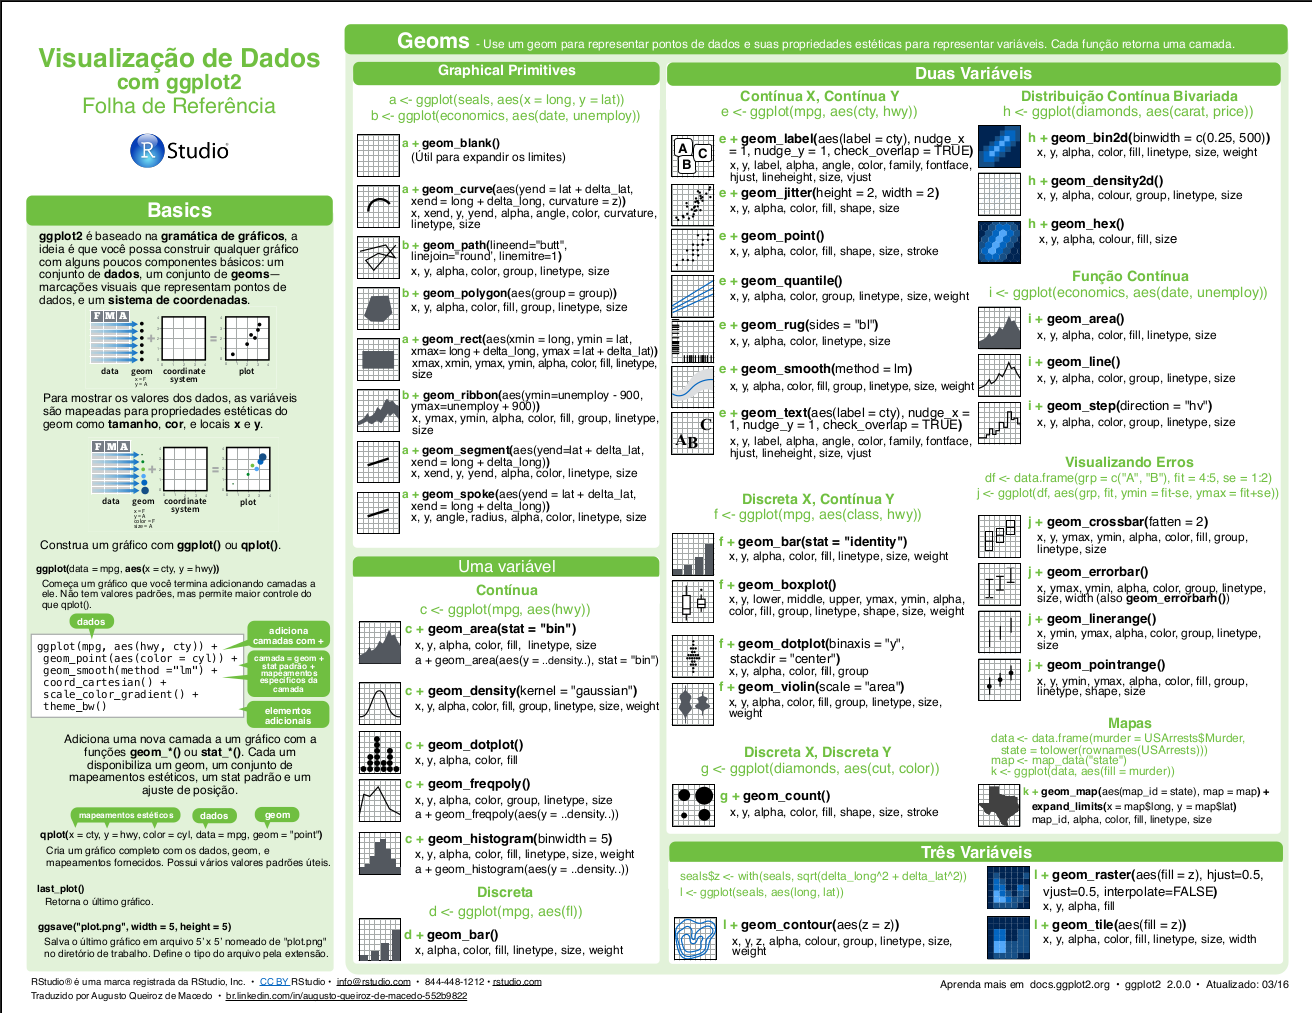
\includegraphics{Visualizacao/images/cs-ggplot-01.png}}

}

\end{figure}

\begin{figure}

{\centering 

\href{images/cs-ggplot-02.png}{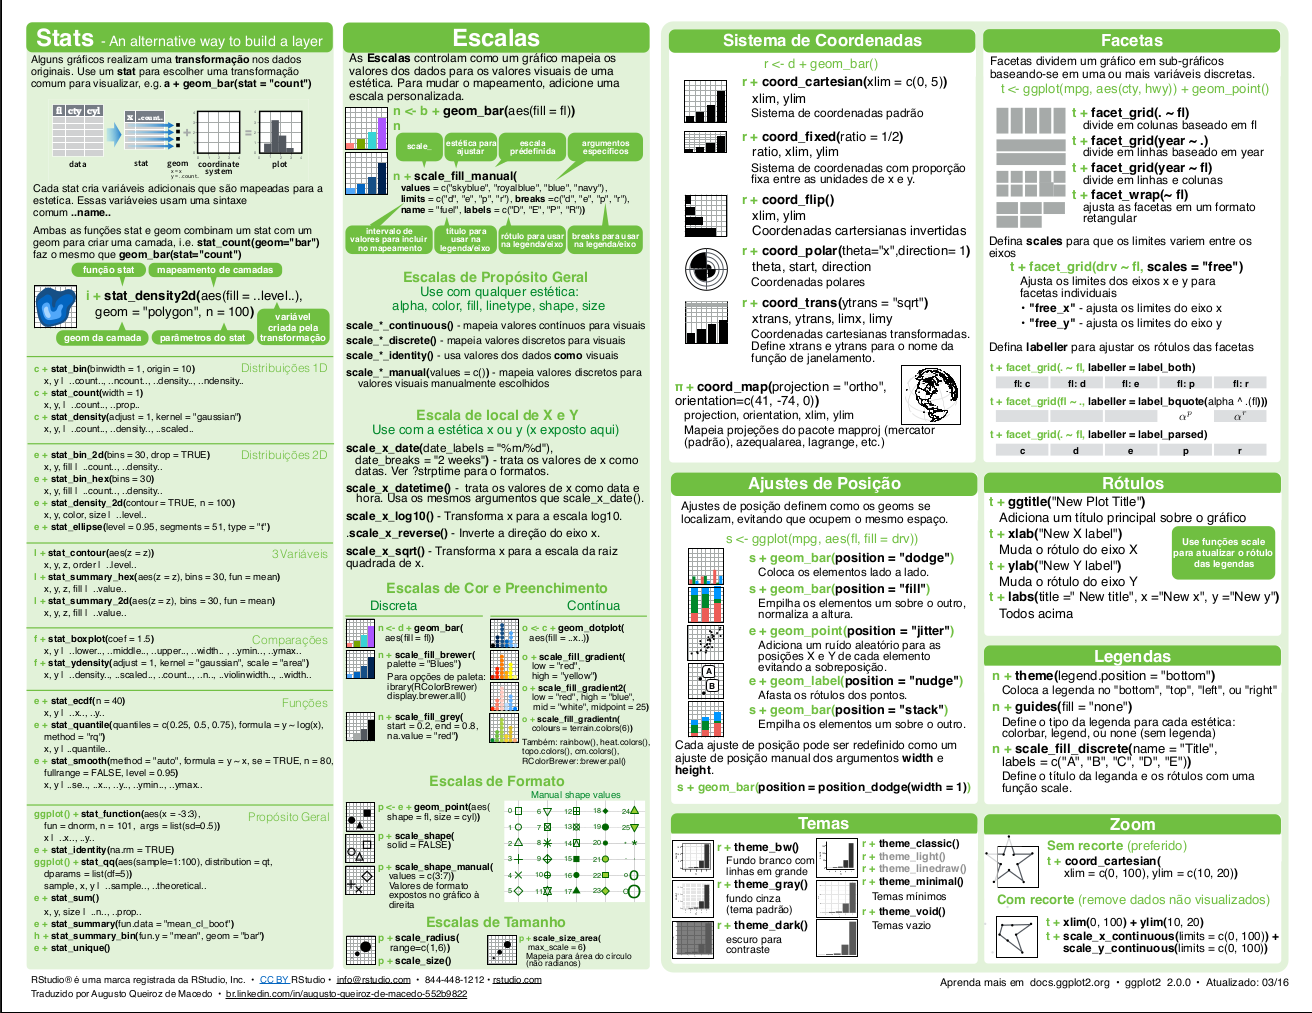
\includegraphics{Visualizacao/images/cs-ggplot-02.png}}

}

\end{figure}

\begin{center}\rule{0.5\linewidth}{0.5pt}\end{center}

\hypertarget{variuxe1veis-discretas-e-contuxednuas-no-ggplot}{%
\subsubsection{Variáveis Discretas e Contínuas no
GGPLOT}\label{variuxe1veis-discretas-e-contuxednuas-no-ggplot}}

O ggplot2, em geral irá associar as variáveis \textbf{caractere} (char)
e \textbf{fatores} (factors) em escalas \textbf{discretas} de forma
automática. Já as variáveis \textbf{numéricas,} o ggplot irá associar
automaticamente com escalas \textbf{contínuas}.

Você verá nas seções seguintes este tipo de segregação, ou seja, um
gráfico para variáveis discretas, contínuas ou um mix de ambas e assim
por diante.

\begin{tcolorbox}[enhanced jigsaw, rightrule=.15mm, arc=.35mm, coltitle=black, colframe=quarto-callout-important-color-frame, opacityback=0, toprule=.15mm, left=2mm, breakable, colback=white, bottomtitle=1mm, leftrule=.75mm, title=\textcolor{quarto-callout-important-color}{\faExclamation}\hspace{0.5em}{Importante}, colbacktitle=quarto-callout-important-color!10!white, titlerule=0mm, bottomrule=.15mm, toptitle=1mm, opacitybacktitle=0.6]
Quando tivermos variáveis que não seguem este padrão, devemos
``transformá-las, usando funções como as\_factor(), as.integer(),
as.double, etc.

Por exemplo, para representar uma variável que é do tipo inteiro, porém
é discreta, deveremos antes alterá-la para um fator antes de submeter ao
ggplot preferencialmente.
\end{tcolorbox}

\hypertarget{gramuxe1tica-dos-gruxe1ficos}{%
\section{Gramática dos Gráficos}\label{gramuxe1tica-dos-gruxe1ficos}}

O pacote ggplot2 é uma implementação do livro ``\textbf{\emph{Grammar of
Graphics}}'', que apresenta um conceito de quais seriam os elementos de
um gráfico e suas interconexões. O modelo teórico proposto no livro é
que através de camadas definidas qualquer gráfico pode ser construído.
Abaixo o modelo, que deve ser interpretado de baixo para cima.

\includegraphics[width=3.6875in,height=\textheight]{Visualizacao/images/grammar-01.jpg}

De uma forma bem resumida, a idéia é que você possa construir
minimamente qualquer gráfico com base nestes mesmos elementos: um
\textbf{conjunto de dados}, um \textbf{sistema de coordenadas} e
\textbf{geometrias}, que seriam marcas visuais que representas os pontos
dos dados.

\includegraphics[width=4.94792in,height=\textheight]{Visualizacao/images/ggplot-01.jpg}

No caso do ggplot2, para mostrar valores no gráfico, as varíaveis do
conjunto de dados podem ser \textbf{mapeadas} em propriedadas visuais da
geometria (geom).

Este mapeamento de estética (aesthetic) é feito através da função aes()
e podemos fazer mapeamentos estéticos como cor, tamanho, forma, etc.

\includegraphics[width=4.94792in,height=\textheight]{Visualizacao/images/ggplot-02.jpg}

\hypertarget{modelo-para-construuxe7uxe3o-de-um-gruxe1fico}{%
\section{Modelo para Construção de um
Gráfico}\label{modelo-para-construuxe7uxe3o-de-um-gruxe1fico}}

No caso do ggplot2, podemos definir uma espécie de modelo (template)
para a sintaxe de construção de gráficos:

\includegraphics[width=5.79167in,height=\textheight]{Visualizacao/images/ggplot_template-01.jpg}

Vejamos a seguir uma introdução ao uso do modelo visto acima:

\begin{center}\rule{0.5\linewidth}{0.5pt}\end{center}

\hypertarget{ggplot}{%
\subsubsection{ggplot}\label{ggplot}}

A função ggplot() inicia um gráfico que será completado com as camadas
adicionadas na sequência, como uma geometria, um sistema de coordenada
ou até um tema.

Usando o modelo acima, vamos gerar nosso primeiro gráfico.

Como base de dados usaremos a tabela \textbf{mtcars}. Para maiores
informação sobre as \textbf{variáveis} (colunas) e \textbf{observações}
(linhas) do mtcars, digite ?mtcars.

\begin{Shaded}
\begin{Highlighting}[]
\NormalTok{mtcars}
\end{Highlighting}
\end{Shaded}

\begin{verbatim}
                     mpg cyl  disp  hp drat    wt  qsec vs am gear carb
Mazda RX4           21.0   6 160.0 110 3.90 2.620 16.46  0  1    4    4
Mazda RX4 Wag       21.0   6 160.0 110 3.90 2.875 17.02  0  1    4    4
Datsun 710          22.8   4 108.0  93 3.85 2.320 18.61  1  1    4    1
Hornet 4 Drive      21.4   6 258.0 110 3.08 3.215 19.44  1  0    3    1
Hornet Sportabout   18.7   8 360.0 175 3.15 3.440 17.02  0  0    3    2
Valiant             18.1   6 225.0 105 2.76 3.460 20.22  1  0    3    1
Duster 360          14.3   8 360.0 245 3.21 3.570 15.84  0  0    3    4
Merc 240D           24.4   4 146.7  62 3.69 3.190 20.00  1  0    4    2
Merc 230            22.8   4 140.8  95 3.92 3.150 22.90  1  0    4    2
Merc 280            19.2   6 167.6 123 3.92 3.440 18.30  1  0    4    4
Merc 280C           17.8   6 167.6 123 3.92 3.440 18.90  1  0    4    4
Merc 450SE          16.4   8 275.8 180 3.07 4.070 17.40  0  0    3    3
Merc 450SL          17.3   8 275.8 180 3.07 3.730 17.60  0  0    3    3
Merc 450SLC         15.2   8 275.8 180 3.07 3.780 18.00  0  0    3    3
Cadillac Fleetwood  10.4   8 472.0 205 2.93 5.250 17.98  0  0    3    4
Lincoln Continental 10.4   8 460.0 215 3.00 5.424 17.82  0  0    3    4
Chrysler Imperial   14.7   8 440.0 230 3.23 5.345 17.42  0  0    3    4
Fiat 128            32.4   4  78.7  66 4.08 2.200 19.47  1  1    4    1
Honda Civic         30.4   4  75.7  52 4.93 1.615 18.52  1  1    4    2
Toyota Corolla      33.9   4  71.1  65 4.22 1.835 19.90  1  1    4    1
Toyota Corona       21.5   4 120.1  97 3.70 2.465 20.01  1  0    3    1
Dodge Challenger    15.5   8 318.0 150 2.76 3.520 16.87  0  0    3    2
AMC Javelin         15.2   8 304.0 150 3.15 3.435 17.30  0  0    3    2
Camaro Z28          13.3   8 350.0 245 3.73 3.840 15.41  0  0    3    4
Pontiac Firebird    19.2   8 400.0 175 3.08 3.845 17.05  0  0    3    2
Fiat X1-9           27.3   4  79.0  66 4.08 1.935 18.90  1  1    4    1
Porsche 914-2       26.0   4 120.3  91 4.43 2.140 16.70  0  1    5    2
Lotus Europa        30.4   4  95.1 113 3.77 1.513 16.90  1  1    5    2
Ford Pantera L      15.8   8 351.0 264 4.22 3.170 14.50  0  1    5    4
Ferrari Dino        19.7   6 145.0 175 3.62 2.770 15.50  0  1    5    6
Maserati Bora       15.0   8 301.0 335 3.54 3.570 14.60  0  1    5    8
Volvo 142E          21.4   4 121.0 109 4.11 2.780 18.60  1  1    4    2
\end{verbatim}

\begin{Shaded}
\begin{Highlighting}[]
\FunctionTok{ggplot}\NormalTok{(}\AttributeTok{data =}\NormalTok{ mtcars) }\SpecialCharTok{+}
  \FunctionTok{geom\_point}\NormalTok{ (}\AttributeTok{mapping =} \FunctionTok{aes}\NormalTok{(}\AttributeTok{x =}\NormalTok{ hp, }\AttributeTok{y =}\NormalTok{ mpg ))}
\end{Highlighting}
\end{Shaded}

\begin{figure}[H]

{\centering \includegraphics{Visualizacao/Visualizacao_de_dados_com_ggplot2_files/figure-pdf/unnamed-chunk-3-1.pdf}

}

\end{figure}

\begin{tcolorbox}[enhanced jigsaw, rightrule=.15mm, arc=.35mm, coltitle=black, colframe=quarto-callout-note-color-frame, opacityback=0, toprule=.15mm, left=2mm, breakable, colback=white, bottomtitle=1mm, leftrule=.75mm, title=\textcolor{quarto-callout-note-color}{\faInfo}\hspace{0.5em}{Nota}, colbacktitle=quarto-callout-note-color!10!white, titlerule=0mm, bottomrule=.15mm, toptitle=1mm, opacitybacktitle=0.6]
Observe que mesmo sem definirmos escalas, temas, transformações
estatísticas ou outras camadas, o gráfico ainda assim foi gerado.

Isto acontece porque o ggplot tem valores padrões dinâmicos que tentam
prover o melhor resultado possível com o mínimo de esforço.
\end{tcolorbox}

\begin{tcolorbox}[enhanced jigsaw, rightrule=.15mm, arc=.35mm, coltitle=black, colframe=quarto-callout-tip-color-frame, opacityback=0, toprule=.15mm, left=2mm, breakable, colback=white, bottomtitle=1mm, leftrule=.75mm, title=\textcolor{quarto-callout-tip-color}{\faLightbulb}\hspace{0.5em}{Dica}, colbacktitle=quarto-callout-tip-color!10!white, titlerule=0mm, bottomrule=.15mm, toptitle=1mm, opacitybacktitle=0.6]
A definição da estética com seu mapeamento, feito neste exemplo na
função de geometria (geom\_point) poderá ser feito também na função
ggplot().
\end{tcolorbox}

Apesar do gráfico final ser similar, a estética mapeamento poderá ser
utilizada pelas funções geom\_*() nas camadas seguintes, sem a
necessidade de repetí-la, caso contrário, ela será restrito apenas
àquela geom() na qual foi declarada. Veja:

\begin{Shaded}
\begin{Highlighting}[]
\FunctionTok{ggplot}\NormalTok{(}\AttributeTok{data =}\NormalTok{ mtcars, }\AttributeTok{mapping =} \FunctionTok{aes}\NormalTok{(}\AttributeTok{x =}\NormalTok{ hp, }\AttributeTok{y =}\NormalTok{ mpg))}\SpecialCharTok{+}
  \FunctionTok{geom\_point}\NormalTok{()}
\end{Highlighting}
\end{Shaded}

\begin{figure}[H]

{\centering \includegraphics{Visualizacao/Visualizacao_de_dados_com_ggplot2_files/figure-pdf/unnamed-chunk-4-1.pdf}

}

\end{figure}

Por ser comum o uso do argumento data = e mapping =, podemos excluídas
do código, deixando-o mais enxuto, porém mais difícil para quem não tem
tanta familiaridade, veja:

\begin{Shaded}
\begin{Highlighting}[]
\FunctionTok{ggplot}\NormalTok{(mtcars,}\FunctionTok{aes}\NormalTok{(}\AttributeTok{x =}\NormalTok{ hp, }\AttributeTok{y =}\NormalTok{ mpg)) }\SpecialCharTok{+}
  \FunctionTok{geom\_point}\NormalTok{()}
\end{Highlighting}
\end{Shaded}

\begin{figure}[H]

{\centering \includegraphics{Visualizacao/Visualizacao_de_dados_com_ggplot2_files/figure-pdf/unnamed-chunk-5-1.pdf}

}

\end{figure}

\hypertarget{last_plot}{%
\subsubsection{last\_plot}\label{last_plot}}

Use para retornar o último gráfico gerado.

\begin{Shaded}
\begin{Highlighting}[]
\FunctionTok{last\_plot}\NormalTok{()}
\end{Highlighting}
\end{Shaded}

\begin{figure}[H]

{\centering \includegraphics{Visualizacao/Visualizacao_de_dados_com_ggplot2_files/figure-pdf/unnamed-chunk-6-1.pdf}

}

\end{figure}

\hypertarget{ggsave}{%
\subsubsection{ggsave}\label{ggsave}}

Use para salvar o gráfico em uma imagem. O tipo de imagem é selecionado
pela extensão do arquivo de saída.

Por exemplo, para salvar o diretório atual um arquivo com o gráfico
chamado ``plot-01.png'' com o formato de imagem ``.PNG'' de tamanho 5x5
centímetros, fazemos:

\begin{Shaded}
\begin{Highlighting}[]
\FunctionTok{ggsave}\NormalTok{(}\StringTok{"plot{-}01.png"}\NormalTok{, }\AttributeTok{width =} \DecValTok{5}\NormalTok{, }\AttributeTok{height =} \DecValTok{5}\NormalTok{, }\AttributeTok{units =} \StringTok{"cm"}\NormalTok{)}
\end{Highlighting}
\end{Shaded}

\hypertarget{camadas}{%
\section{Camadas}\label{camadas}}

\hypertarget{introduuxe7uxe3o-12}{%
\subsection{Introdução}\label{introduuxe7uxe3o-12}}

A seguir iremos apresentar as principais camadas do ggplot e suas
principais funções.

\begin{tcolorbox}[enhanced jigsaw, rightrule=.15mm, arc=.35mm, coltitle=black, colframe=quarto-callout-note-color-frame, opacityback=0, toprule=.15mm, left=2mm, breakable, colback=white, bottomtitle=1mm, leftrule=.75mm, title=\textcolor{quarto-callout-note-color}{\faInfo}\hspace{0.5em}{Nota}, colbacktitle=quarto-callout-note-color!10!white, titlerule=0mm, bottomrule=.15mm, toptitle=1mm, opacitybacktitle=0.6]
Para a camada de \textbf{dados}, o ggplot aceitará qualquer conjunto de
dados (data frame). Para facilitar a criação do gráfico recomenda-se que
os dados já estejam organizados (\textbf{tidy}) com observações em
linhas e variáveis em colunas.
\end{tcolorbox}

\begin{itemize}
\item
  Estéticas
\item
  Geometrias
\item
  Estatísticas
\item
  Escalas
\item
  Coordenadas
\item
  Facetas
\item
  Tema
\end{itemize}

\hypertarget{estuxe9ticas}{%
\subsection{Estéticas}\label{estuxe9ticas}}

Podemos mapear a estética de uma camada à variáveis presentes em nossa
camada de dados até definí-las manualmente. Se não especificarmos de
forma explícita, o ggplot tentará assumir valores padrões que serão
usados por determinada função outras camadas, como a de geometria ou de
estatística.

Existem estéticas que são comuns a quase todas as camadas, como
\textbf{cor}, \textbf{forma}, \textbf{tamanho}, etc.

A estética é vinculada à uma variável através da função
\textbf{\emph{aes}}(). É comum, apesar de não ser mandatório para todas
as estéticas, que determinemos os valores para x e y.

A seguir veremos algumas delas:

\hypertarget{color-e-fill}{%
\subsubsection{color e fill}\label{color-e-fill}}

Use para definir a \textbf{cor} (color) ou \textbf{preenchimento} (fill)
para a estética.

\begin{Shaded}
\begin{Highlighting}[]
\FunctionTok{ggplot}\NormalTok{(mtcars)}\SpecialCharTok{+}
  \FunctionTok{geom\_point}\NormalTok{(}\FunctionTok{aes}\NormalTok{(}\AttributeTok{x =}\NormalTok{ hp, }\AttributeTok{y =}\NormalTok{ mpg, }\AttributeTok{color =} \StringTok{"red"}\NormalTok{))}
\end{Highlighting}
\end{Shaded}

\begin{figure}[H]

{\centering \includegraphics{Visualizacao/Visualizacao_de_dados_com_ggplot2_files/figure-pdf/unnamed-chunk-8-1.pdf}

}

\end{figure}

No exemplo acima, definimos que a estética ``\textbf{x}'', assumirá
valores provenientes da variável que existe em nossos dados chamada
``\textbf{hp}''. Já a estética ``\textbf{y}'', assumirá valores
provenientes da variável ``\textbf{mpg}''.

Já a estética ``color'' assumirá o valor constante ``red''. Na string de
color =, podemos usar valores de cores em inglês, como ``red'' ou
``blue'', ou também códigos RGB, como ````\#00ABFF'' ou ``FF00AA''.

\begin{tcolorbox}[enhanced jigsaw, rightrule=.15mm, arc=.35mm, coltitle=black, colframe=quarto-callout-important-color-frame, opacityback=0, toprule=.15mm, left=2mm, breakable, colback=white, bottomtitle=1mm, leftrule=.75mm, title=\textcolor{quarto-callout-important-color}{\faExclamation}\hspace{0.5em}{Importante}, colbacktitle=quarto-callout-important-color!10!white, titlerule=0mm, bottomrule=.15mm, toptitle=1mm, opacitybacktitle=0.6]
Observe que o valor definido da cor, foi dentro dos parênteses da função
aes(), ou seja, ela está fazendo o mapeamento da estética cor (color)
com os dados. Se utilizarmos o argumento color = da função
geom\_point(),estaremos definindo um valor fora do mapeamento.
\end{tcolorbox}

\begin{Shaded}
\begin{Highlighting}[]
\FunctionTok{ggplot}\NormalTok{(mtcars)}\SpecialCharTok{+}
  \FunctionTok{geom\_point}\NormalTok{(}\FunctionTok{aes}\NormalTok{(}\AttributeTok{x =}\NormalTok{ hp, }\AttributeTok{y =}\NormalTok{ mpg) , }\AttributeTok{color =} \StringTok{"red"}\NormalTok{)}
\end{Highlighting}
\end{Shaded}

\begin{figure}[H]

{\centering \includegraphics{Visualizacao/Visualizacao_de_dados_com_ggplot2_files/figure-pdf/unnamed-chunk-9-1.pdf}

}

\end{figure}

Apesar do resultado ser similar, observe que no exemplo anterior tivemos
color como um mapeamento da estética, como definimos o valor fixo com a
cor ``red'', seria como tivessemos em nossos dados uma coluna onde todas
as linhas tivessem o valor ``red''. Já no exemplo acima, estamos
simplemente dizendo à função da geometria que queremos a cor vermelha
para ela.

Vejamos um outro exemplo para que fique claro este ponto.

Vamos gerar o mesmo gráfico onde colocamos ``red'' como parte da
estética, porém agora, iremos mapeá-la com a coluna ``qsec'' de nossos
dados mtcars:

\begin{Shaded}
\begin{Highlighting}[]
\FunctionTok{ggplot}\NormalTok{(mtcars)}\SpecialCharTok{+}
  \FunctionTok{geom\_point}\NormalTok{(}\FunctionTok{aes}\NormalTok{(}\AttributeTok{x =}\NormalTok{ hp, }\AttributeTok{y =}\NormalTok{ mpg, }\AttributeTok{color =}\NormalTok{ qsec))}
\end{Highlighting}
\end{Shaded}

\begin{figure}[H]

{\centering \includegraphics{Visualizacao/Visualizacao_de_dados_com_ggplot2_files/figure-pdf/unnamed-chunk-10-1.pdf}

}

\end{figure}

Observe que neste caso a estética de cor foi mapeada com a variável
qsec. Por se tratar de uma variável contínua, o ggplot escolheu
autometicamente uma sequência de cores, neste caso do azul claro para o
azul escuro, para representar este tipo de variável. Veremos mais
adiante como customizar esta e outras escolhar automáticas feitas nas
escalas.

\hypertarget{linetype}{%
\subsubsection{linetype}\label{linetype}}

Use para definir a linha utilizada no gráfico. Podemos utilizar um
número de 0 a 6 ou um nome:

\emph{(0 = ``blank'', 1 = ``solid'', 2 = ``dashed'', 3 = ``dotted'', 4 =
``dotdash'', 5 = ``longdash'',6 = ``twodash'')}

Por exemplo, ao invés de utilizarmos a geometria de pontos
(geom\_point), vamos utilzar a geometria de linha (geom\_line):

\begin{Shaded}
\begin{Highlighting}[]
\FunctionTok{ggplot}\NormalTok{(mtcars)}\SpecialCharTok{+}
  \FunctionTok{geom\_line}\NormalTok{(}\FunctionTok{aes}\NormalTok{(}\AttributeTok{x =}\NormalTok{ hp, }\AttributeTok{y =}\NormalTok{ mpg) , }\AttributeTok{linetype =} \StringTok{"dotted"}\NormalTok{)}
\end{Highlighting}
\end{Shaded}

\begin{figure}[H]

{\centering \includegraphics{Visualizacao/Visualizacao_de_dados_com_ggplot2_files/figure-pdf/unnamed-chunk-11-1.pdf}

}

\end{figure}

\hypertarget{size}{%
\subsubsection{size}\label{size}}

Use para definir o tamanho, no caso de uma linha em ``mm''.

Como dito anteriormente, estes valores são comuns para vários
geometrias. Por exemplo, podemos utilizar o argumento size também na
geometria de pontos (geom\_point):

\begin{Shaded}
\begin{Highlighting}[]
\FunctionTok{ggplot}\NormalTok{(mtcars)}\SpecialCharTok{+}
  \FunctionTok{geom\_line}\NormalTok{(}\FunctionTok{aes}\NormalTok{(}\AttributeTok{x =}\NormalTok{ hp, }\AttributeTok{y =}\NormalTok{ mpg), }\AttributeTok{size =} \DecValTok{5}\NormalTok{)}
\FunctionTok{ggplot}\NormalTok{(mtcars)}\SpecialCharTok{+}
  \FunctionTok{geom\_point}\NormalTok{(}\FunctionTok{aes}\NormalTok{(}\AttributeTok{x =}\NormalTok{ hp, }\AttributeTok{y =}\NormalTok{ mpg), }\AttributeTok{size =} \DecValTok{5}\NormalTok{)}
\end{Highlighting}
\end{Shaded}

\begin{figure}

\begin{minipage}[t]{0.50\linewidth}

{\centering 

\raisebox{-\height}{

\includegraphics{Visualizacao/Visualizacao_de_dados_com_ggplot2_files/figure-pdf/unnamed-chunk-12-1.pdf}

}

}

\end{minipage}%
%
\begin{minipage}[t]{0.50\linewidth}

{\centering 

\raisebox{-\height}{

\includegraphics{Visualizacao/Visualizacao_de_dados_com_ggplot2_files/figure-pdf/unnamed-chunk-12-2.pdf}

}

}

\end{minipage}%

\end{figure}

\hypertarget{lineend}{%
\subsubsection{lineend}\label{lineend}}

Use para definir o terminador da linha. Os valores podem ser:
\emph{round}, \emph{butt} e \emph{square}.

\hypertarget{squared}{%
\subsubsection{squared}\label{squared}}

\begin{Shaded}
\begin{Highlighting}[]
\FunctionTok{ggplot}\NormalTok{(mtcars)}\SpecialCharTok{+}
  \FunctionTok{geom\_line}\NormalTok{(}\FunctionTok{aes}\NormalTok{(}\AttributeTok{x =}\NormalTok{ hp, }\AttributeTok{y =}\NormalTok{ mpg), }\AttributeTok{lineend =} \StringTok{"square"}\NormalTok{, }\AttributeTok{size =} \DecValTok{4}\NormalTok{)}
\end{Highlighting}
\end{Shaded}

\begin{figure}[H]

{\centering \includegraphics{Visualizacao/Visualizacao_de_dados_com_ggplot2_files/figure-pdf/unnamed-chunk-13-1.pdf}

}

\end{figure}

\hypertarget{butt}{%
\subsubsection{butt}\label{butt}}

\begin{Shaded}
\begin{Highlighting}[]
\FunctionTok{ggplot}\NormalTok{(mtcars)}\SpecialCharTok{+}
  \FunctionTok{geom\_line}\NormalTok{(}\FunctionTok{aes}\NormalTok{(}\AttributeTok{x =}\NormalTok{ hp, }\AttributeTok{y =}\NormalTok{ mpg), }\AttributeTok{lineend =} \StringTok{"butt"}\NormalTok{, }\AttributeTok{size =} \DecValTok{4}\NormalTok{)}
\end{Highlighting}
\end{Shaded}

\begin{figure}[H]

{\centering \includegraphics{Visualizacao/Visualizacao_de_dados_com_ggplot2_files/figure-pdf/unnamed-chunk-14-1.pdf}

}

\end{figure}

\hypertarget{round}{%
\subsubsection{round}\label{round}}

\begin{Shaded}
\begin{Highlighting}[]
\FunctionTok{ggplot}\NormalTok{(mtcars)}\SpecialCharTok{+}
  \FunctionTok{geom\_line}\NormalTok{(}\FunctionTok{aes}\NormalTok{(}\AttributeTok{x =}\NormalTok{ hp, }\AttributeTok{y =}\NormalTok{ mpg), }\AttributeTok{lineend =} \StringTok{"round"}\NormalTok{, }\AttributeTok{size =} \DecValTok{4}\NormalTok{)}
\end{Highlighting}
\end{Shaded}

\begin{figure}[H]

{\centering \includegraphics{Visualizacao/Visualizacao_de_dados_com_ggplot2_files/figure-pdf/unnamed-chunk-15-1.pdf}

}

\end{figure}

\hypertarget{linejoin}{%
\subsubsection{linejoin}\label{linejoin}}

Use para definir a junção da linha. Os valores podem ser: \emph{round},
\emph{mitre} e \emph{bevel}.

\hypertarget{round-1}{%
\subsubsection{round}\label{round-1}}

\begin{Shaded}
\begin{Highlighting}[]
\FunctionTok{ggplot}\NormalTok{(mtcars)}\SpecialCharTok{+}
  \FunctionTok{geom\_line}\NormalTok{(}\FunctionTok{aes}\NormalTok{(}\AttributeTok{x =}\NormalTok{ hp, }\AttributeTok{y =}\NormalTok{ mpg), }\AttributeTok{linejoin =} \StringTok{"round"}\NormalTok{, }\AttributeTok{size =} \DecValTok{4}\NormalTok{)}
\end{Highlighting}
\end{Shaded}

\begin{figure}[H]

{\centering \includegraphics{Visualizacao/Visualizacao_de_dados_com_ggplot2_files/figure-pdf/unnamed-chunk-16-1.pdf}

}

\end{figure}

\hypertarget{mitre}{%
\subsubsection{mitre}\label{mitre}}

\begin{Shaded}
\begin{Highlighting}[]
\FunctionTok{ggplot}\NormalTok{(mtcars)}\SpecialCharTok{+}
  \FunctionTok{geom\_line}\NormalTok{(}\FunctionTok{aes}\NormalTok{(}\AttributeTok{x =}\NormalTok{ hp, }\AttributeTok{y =}\NormalTok{ mpg), }\AttributeTok{linejoin =} \StringTok{"mitre"}\NormalTok{, }\AttributeTok{size =} \DecValTok{4}\NormalTok{)}
\end{Highlighting}
\end{Shaded}

\begin{figure}[H]

{\centering \includegraphics{Visualizacao/Visualizacao_de_dados_com_ggplot2_files/figure-pdf/unnamed-chunk-17-1.pdf}

}

\end{figure}

\hypertarget{bevel}{%
\subsubsection{bevel}\label{bevel}}

\begin{Shaded}
\begin{Highlighting}[]
\FunctionTok{ggplot}\NormalTok{(mtcars)}\SpecialCharTok{+}
  \FunctionTok{geom\_line}\NormalTok{(}\FunctionTok{aes}\NormalTok{(}\AttributeTok{x =}\NormalTok{ hp, }\AttributeTok{y =}\NormalTok{ mpg), }\AttributeTok{linejoin =} \StringTok{"bevel"}\NormalTok{, }\AttributeTok{size =} \DecValTok{4}\NormalTok{)}
\end{Highlighting}
\end{Shaded}

\begin{figure}[H]

{\centering \includegraphics{Visualizacao/Visualizacao_de_dados_com_ggplot2_files/figure-pdf/unnamed-chunk-18-1.pdf}

}

\end{figure}

\hypertarget{shape}{%
\subsubsection{shape}\label{shape}}

Use para definir a forma. Podemos passar um número ou um nome em inglês
da forma conforme abaixo:

\includegraphics{Visualizacao/images/aes_shape-01.jpg}

\begin{Shaded}
\begin{Highlighting}[]
\FunctionTok{ggplot}\NormalTok{(mtcars)}\SpecialCharTok{+}
  \FunctionTok{geom\_point}\NormalTok{(}\FunctionTok{aes}\NormalTok{(}\AttributeTok{x =}\NormalTok{ hp, }\AttributeTok{y =}\NormalTok{ mpg), }\AttributeTok{shape =} \StringTok{"square cross"}\NormalTok{,  }\AttributeTok{size =} \DecValTok{3}\NormalTok{)}
\FunctionTok{ggplot}\NormalTok{(mtcars)}\SpecialCharTok{+}
  \FunctionTok{geom\_point}\NormalTok{(}\FunctionTok{aes}\NormalTok{(}\AttributeTok{x =}\NormalTok{ hp, }\AttributeTok{y =}\NormalTok{ mpg), }\AttributeTok{shape =} \DecValTok{5}\NormalTok{, }\AttributeTok{size =} \DecValTok{3}\NormalTok{)}
\end{Highlighting}
\end{Shaded}

\begin{figure}

\begin{minipage}[t]{0.50\linewidth}

{\centering 

\raisebox{-\height}{

\includegraphics{Visualizacao/Visualizacao_de_dados_com_ggplot2_files/figure-pdf/unnamed-chunk-19-1.pdf}

}

}

\end{minipage}%
%
\begin{minipage}[t]{0.50\linewidth}

{\centering 

\raisebox{-\height}{

\includegraphics{Visualizacao/Visualizacao_de_dados_com_ggplot2_files/figure-pdf/unnamed-chunk-19-2.pdf}

}

}

\end{minipage}%

\end{figure}

\hypertarget{geometrias-geoms}{%
\subsection{Geometrias}\label{geometrias-geoms}}

O ggplot nos permite selecionar para o mesmo gráfico uma ou mais formas
geométrias. Por exemplo, eu posso ter o mesmo gráfico final, mas ao
invés de ter pontos representando os dados, podemos ter barras e assim
por diante.

\begin{tcolorbox}[enhanced jigsaw, rightrule=.15mm, arc=.35mm, coltitle=black, colframe=quarto-callout-warning-color-frame, opacityback=0, toprule=.15mm, left=2mm, breakable, colback=white, bottomtitle=1mm, leftrule=.75mm, title=\textcolor{quarto-callout-warning-color}{\faExclamationTriangle}\hspace{0.5em}{Aviso}, colbacktitle=quarto-callout-warning-color!10!white, titlerule=0mm, bottomrule=.15mm, toptitle=1mm, opacitybacktitle=0.6]
Lembre-se que cada função retornará uma camada, portanto, a ordem de
criação das camadas afeta o resultado do gráfico, pois uma será criada
sobre a anterior.
\end{tcolorbox}

\hypertarget{gruxe1ficos-primitivos}{%
\subsubsection{\texorpdfstring{\textbf{Gráficos
Primitivos}}{Gráficos Primitivos}}\label{gruxe1ficos-primitivos}}

Para os exemplos a seguir, utilizaremos duas bases de dados, uma chamada
\textbf{economics} e outra chamada \textbf{seals}.

\hypertarget{economics}{%
\subsubsection{Economics}\label{economics}}

\begin{Shaded}
\begin{Highlighting}[]
\NormalTok{economics}
\end{Highlighting}
\end{Shaded}

\begin{verbatim}
# A tibble: 574 x 6
   date         pce    pop psavert uempmed unemploy
   <date>     <dbl>  <dbl>   <dbl>   <dbl>    <dbl>
 1 1967-07-01  507. 198712    12.6     4.5     2944
 2 1967-08-01  510. 198911    12.6     4.7     2945
 3 1967-09-01  516. 199113    11.9     4.6     2958
 4 1967-10-01  512. 199311    12.9     4.9     3143
 5 1967-11-01  517. 199498    12.8     4.7     3066
 6 1967-12-01  525. 199657    11.8     4.8     3018
 7 1968-01-01  531. 199808    11.7     5.1     2878
 8 1968-02-01  534. 199920    12.3     4.5     3001
 9 1968-03-01  544. 200056    11.7     4.1     2877
10 1968-04-01  544  200208    12.3     4.6     2709
# ... with 564 more rows
# i Use `print(n = ...)` to see more rows
\end{verbatim}

\hypertarget{seals}{%
\subsubsection{Seals}\label{seals}}

\begin{Shaded}
\begin{Highlighting}[]
\NormalTok{seals}
\end{Highlighting}
\end{Shaded}

\begin{verbatim}
# A tibble: 1,155 x 4
     lat  long delta_long delta_lat
   <dbl> <dbl>      <dbl>     <dbl>
 1  29.7 -173.     -0.915   0.143  
 2  30.7 -173.     -0.867   0.128  
 3  31.7 -173.     -0.819   0.113  
 4  32.7 -173.     -0.771   0.0980 
 5  33.7 -173.     -0.723   0.0828 
 6  34.7 -173.     -0.674   0.0675 
 7  35.7 -173.     -0.626   0.0522 
 8  36.7 -173.     -0.577   0.0369 
 9  37.7 -173.     -0.529   0.0216 
10  38.7 -173.     -0.480   0.00635
# ... with 1,145 more rows
# i Use `print(n = ...)` to see more rows
\end{verbatim}

Para simplificar o código dos próximos exemplos, iremos criar dois
objetos gráfico do ggplot:

O primeiro chamado ``\textbf{a}'', irá conter um objeto ggplot com os
dados de \textbf{economics}, mapeando a estética de \textbf{x} para a
variável ``\textbf{date}'' e \textbf{y} para a variável
``\textbf{unemployed}''.

O segundo chamado ``\textbf{b}'', irá conter um objeto ggplot com os
dados de \textbf{seals}, mapeando a estética de \textbf{x} para a
\textbf{variável} ``\textbf{long}'' e \textbf{y} para a variável
``\textbf{lat}''.

Desta forma trabalharemos com os mesmos objetos base e adicionaremos
apenas novas camadas utilizando o operador ``\textbf{+}'' a fim de
identificar os detalhes das diversas funções de geometria e não
precisarmos repetir o código das camadas iniciais do gráfico.

\begin{Shaded}
\begin{Highlighting}[]
\NormalTok{a }\OtherTok{\textless{}{-}} \FunctionTok{ggplot}\NormalTok{(economics, }\FunctionTok{aes}\NormalTok{(date, unemploy))}
\NormalTok{b }\OtherTok{\textless{}{-}} \FunctionTok{ggplot}\NormalTok{(seals, }\FunctionTok{aes}\NormalTok{(}\AttributeTok{x =}\NormalTok{ long, }\AttributeTok{y =}\NormalTok{ lat))}
\end{Highlighting}
\end{Shaded}

\begin{tcolorbox}[enhanced jigsaw, rightrule=.15mm, arc=.35mm, coltitle=black, colframe=quarto-callout-note-color-frame, opacityback=0, toprule=.15mm, left=2mm, breakable, colback=white, bottomtitle=1mm, leftrule=.75mm, title=\textcolor{quarto-callout-note-color}{\faInfo}\hspace{0.5em}{Nota}, colbacktitle=quarto-callout-note-color!10!white, titlerule=0mm, bottomrule=.15mm, toptitle=1mm, opacitybacktitle=0.6]
Para simplificar o código, em algum momentos podemos omitir o argumento,
como data=, mapping = , x = , y = . Isto porque já estamos os valores na
ordem que a função nos pede.
\end{tcolorbox}

Agora com os objetos inicialmente criados, iremos adicionar novas
camadas afim de obtermos os gráficos e entendermos algumas das funções
de geometria para gráficos primitivos.

\hypertarget{geom_blank}{%
\subsubsection{geom\_blank}\label{geom_blank}}

Use para garantir limites para todos os gráficos de acordo com os dados.

\begin{Shaded}
\begin{Highlighting}[]
\NormalTok{a }\SpecialCharTok{+} \FunctionTok{geom\_blank}\NormalTok{()}
\end{Highlighting}
\end{Shaded}

\begin{figure}[H]

{\centering \includegraphics{Visualizacao/Visualizacao_de_dados_com_ggplot2_files/figure-pdf/unnamed-chunk-23-1.pdf}

}

\end{figure}

\begin{tcolorbox}[enhanced jigsaw, rightrule=.15mm, arc=.35mm, coltitle=black, colframe=quarto-callout-tip-color-frame, opacityback=0, toprule=.15mm, left=2mm, breakable, colback=white, bottomtitle=1mm, leftrule=.75mm, title=\textcolor{quarto-callout-tip-color}{\faLightbulb}\hspace{0.5em}{Dica}, colbacktitle=quarto-callout-tip-color!10!white, titlerule=0mm, bottomrule=.15mm, toptitle=1mm, opacitybacktitle=0.6]
Use a função \textbf{expand\_limits}() para expandir os limites do
gráfico usando dados. Ver ?expand\_limits para mais detalhes.
\end{tcolorbox}

\hypertarget{geom_curve}{%
\subsubsection{geom\_curve}\label{geom_curve}}

Use para criar curvas.

\begin{Shaded}
\begin{Highlighting}[]
\NormalTok{b }\SpecialCharTok{+} \FunctionTok{geom\_curve}\NormalTok{(}\FunctionTok{aes}\NormalTok{(}\AttributeTok{yend =}\NormalTok{ lat }\SpecialCharTok{+} \DecValTok{1}\NormalTok{, }\AttributeTok{xend =}\NormalTok{ long }\SpecialCharTok{+} \DecValTok{1}\NormalTok{), }\AttributeTok{curvature =} \DecValTok{1}\NormalTok{)}
\end{Highlighting}
\end{Shaded}

\begin{figure}[H]

{\centering \includegraphics{Visualizacao/Visualizacao_de_dados_com_ggplot2_files/figure-pdf/unnamed-chunk-24-1.pdf}

}

\end{figure}

\hypertarget{geom_path}{%
\subsubsection{geom\_path}\label{geom_path}}

Use para conectar observações.

\begin{Shaded}
\begin{Highlighting}[]
\NormalTok{a }\SpecialCharTok{+} \FunctionTok{geom\_path}\NormalTok{(}\AttributeTok{lineend =} \StringTok{"butt"}\NormalTok{, }\AttributeTok{linejoin =} \StringTok{"round"}\NormalTok{, }\AttributeTok{linemitre =} \DecValTok{1}\NormalTok{)}
\end{Highlighting}
\end{Shaded}

\begin{figure}[H]

{\centering \includegraphics{Visualizacao/Visualizacao_de_dados_com_ggplot2_files/figure-pdf/unnamed-chunk-25-1.pdf}

}

\end{figure}

\hypertarget{geom_polygon}{%
\subsubsection{geom\_polygon}\label{geom_polygon}}

Use para criar poligonos. É similar a geom\_path(), porém a parte
interna é preenchida com argumento fill =.

\begin{Shaded}
\begin{Highlighting}[]
\NormalTok{a }\SpecialCharTok{+} \FunctionTok{geom\_polygon}\NormalTok{(}\FunctionTok{aes}\NormalTok{(}\AttributeTok{alpha =} \DecValTok{50}\NormalTok{))}
\end{Highlighting}
\end{Shaded}

\begin{figure}[H]

{\centering \includegraphics{Visualizacao/Visualizacao_de_dados_com_ggplot2_files/figure-pdf/unnamed-chunk-26-1.pdf}

}

\end{figure}

\begin{tcolorbox}[enhanced jigsaw, rightrule=.15mm, arc=.35mm, coltitle=black, colframe=quarto-callout-note-color-frame, opacityback=0, toprule=.15mm, left=2mm, breakable, colback=white, bottomtitle=1mm, leftrule=.75mm, title=\textcolor{quarto-callout-note-color}{\faInfo}\hspace{0.5em}{Nota}, colbacktitle=quarto-callout-note-color!10!white, titlerule=0mm, bottomrule=.15mm, toptitle=1mm, opacitybacktitle=0.6]
O argumento alpha = , é muito comum na definição de cores. De maneira
simplificada, ele indica o nível de transparência de uma cor, sendo 0,
nenhuma transparência e 1 transparência total.
\end{tcolorbox}

\hypertarget{geom_rect}{%
\subsubsection{geom\_rect}\label{geom_rect}}

Use para criar retângulos.

\begin{Shaded}
\begin{Highlighting}[]
\NormalTok{b }\SpecialCharTok{+} \FunctionTok{geom\_rect}\NormalTok{(}\FunctionTok{aes}\NormalTok{(}\AttributeTok{xmin =}\NormalTok{ long, }\AttributeTok{ymin =}\NormalTok{ lat,}
\AttributeTok{xmax =}\NormalTok{ long }\SpecialCharTok{+} \DecValTok{1}\NormalTok{, }\AttributeTok{ymax =}\NormalTok{ lat }\SpecialCharTok{+} \DecValTok{1}\NormalTok{))}
\end{Highlighting}
\end{Shaded}

\begin{figure}[H]

{\centering \includegraphics{Visualizacao/Visualizacao_de_dados_com_ggplot2_files/figure-pdf/unnamed-chunk-27-1.pdf}

}

\end{figure}

\begin{tcolorbox}[enhanced jigsaw, rightrule=.15mm, arc=.35mm, coltitle=black, colframe=quarto-callout-note-color-frame, opacityback=0, toprule=.15mm, left=2mm, breakable, colback=white, bottomtitle=1mm, leftrule=.75mm, title=\textcolor{quarto-callout-note-color}{\faInfo}\hspace{0.5em}{Nota}, colbacktitle=quarto-callout-note-color!10!white, titlerule=0mm, bottomrule=.15mm, toptitle=1mm, opacitybacktitle=0.6]
A função \textbf{geom\_title()} fazem a mesma coisa, porém são
parametrizadas de forma diferente. A geom\_rect usa a localização dos 4
cantos do quadrado, enquanto a geom\_tile usa o centro e seu tamanho
(largura e altura) para dimensionar.
\end{tcolorbox}

\hypertarget{geom_ribbon}{%
\subsubsection{geom\_ribbon}\label{geom_ribbon}}

Use para criar uma ``fita''. Para cada valor de x, ela mostra um
intervalo y, definido por ymin e ymax. Veja que geom\_area() é um caso
especial do geom\_ribbon(), onde o ymin é fixo em 0 e y é usado no lugar
de ymax.

\begin{Shaded}
\begin{Highlighting}[]
\NormalTok{a }\SpecialCharTok{+} \FunctionTok{geom\_ribbon}\NormalTok{ (}\FunctionTok{aes}\NormalTok{(}\AttributeTok{ymin =}\NormalTok{ unemploy }\SpecialCharTok{{-}} \DecValTok{900}\NormalTok{,}
\AttributeTok{ymax =}\NormalTok{ unemploy }\SpecialCharTok{+} \DecValTok{900}\NormalTok{))}
\end{Highlighting}
\end{Shaded}

\begin{figure}[H]

{\centering \includegraphics{Visualizacao/Visualizacao_de_dados_com_ggplot2_files/figure-pdf/unnamed-chunk-28-1.pdf}

}

\end{figure}

\hypertarget{segmentos-de-linhas}{%
\subsubsection{\texorpdfstring{\textbf{Segmentos de
Linhas}}{Segmentos de Linhas}}\label{segmentos-de-linhas}}

Estas funções de geometrias, permitem criar diversos tipo de segmentos
de linha e são úteis quando precisamos ``marcar'' ou definir algo no
gráfico, com linhas verticais ou horizontais por exemplo.

\hypertarget{geom_abline}{%
\subsubsection{geom\_abline}\label{geom_abline}}

Use para criar uma linha de um ponto ``a'' até um ponto ``b'', passando
o intercepto e a inclinação da reta.

\begin{Shaded}
\begin{Highlighting}[]
\NormalTok{b }\SpecialCharTok{+}  \FunctionTok{geom\_abline}\NormalTok{(}\FunctionTok{aes}\NormalTok{(}\AttributeTok{intercept =} \DecValTok{0}\NormalTok{, }\AttributeTok{slope =} \DecValTok{1}\NormalTok{))}
\end{Highlighting}
\end{Shaded}

\begin{figure}[H]

{\centering \includegraphics{Visualizacao/Visualizacao_de_dados_com_ggplot2_files/figure-pdf/unnamed-chunk-29-1.pdf}

}

\end{figure}

\hypertarget{geom_hline}{%
\subsubsection{geom\_hline}\label{geom_hline}}

Use para criar uma ou mais linhas horizontais.

\begin{Shaded}
\begin{Highlighting}[]
\NormalTok{b }\SpecialCharTok{+} \FunctionTok{geom\_hline}\NormalTok{(}\FunctionTok{aes}\NormalTok{(}\AttributeTok{yintercept =}\NormalTok{ lat))}
\end{Highlighting}
\end{Shaded}

\begin{figure}[H]

{\centering \includegraphics{Visualizacao/Visualizacao_de_dados_com_ggplot2_files/figure-pdf/unnamed-chunk-30-1.pdf}

}

\end{figure}

Veja que no exemplo anterior, fizemos o mapeamento do argumento
yintercept como parte da estética (aes), mapeando este argumento com a
variável ``lat'' de nossos dados.

Se quisermos simplesmente traçar uma linha com o intercepto do eixo y,
correspondendo ao valor 40 (por exemplo, se fosse um tipo de meta),
podemos definir este valor fora do mapeamento:

\begin{Shaded}
\begin{Highlighting}[]
\NormalTok{b }\SpecialCharTok{+} \FunctionTok{geom\_hline}\NormalTok{(}\AttributeTok{yintercept =} \DecValTok{40}\NormalTok{)}
\end{Highlighting}
\end{Shaded}

\begin{figure}[H]

{\centering \includegraphics{Visualizacao/Visualizacao_de_dados_com_ggplot2_files/figure-pdf/unnamed-chunk-31-1.pdf}

}

\end{figure}

\hypertarget{geom_vline}{%
\subsubsection{geom\_vline}\label{geom_vline}}

Use para criar uma ou mais linhas horizontais.

\begin{Shaded}
\begin{Highlighting}[]
\NormalTok{b }\SpecialCharTok{+} \FunctionTok{geom\_vline}\NormalTok{(}\FunctionTok{aes}\NormalTok{(}\AttributeTok{xintercept =}\NormalTok{ long))}
\end{Highlighting}
\end{Shaded}

\begin{figure}[H]

{\centering \includegraphics{Visualizacao/Visualizacao_de_dados_com_ggplot2_files/figure-pdf/unnamed-chunk-32-1.pdf}

}

\end{figure}

\hypertarget{geom_segment}{%
\subsubsection{geom\_segment}\label{geom_segment}}

É similar ao geom\_curve, porém ao invés de criar uma curva, criar um
segmento de reta.

\begin{Shaded}
\begin{Highlighting}[]
\NormalTok{b }\SpecialCharTok{+} \FunctionTok{geom\_segment}\NormalTok{(}\FunctionTok{aes}\NormalTok{(}\AttributeTok{yend =}\NormalTok{ lat }\SpecialCharTok{+} \DecValTok{1}\NormalTok{, }\AttributeTok{xend =}\NormalTok{ long }\SpecialCharTok{+} \DecValTok{1}\NormalTok{))}
\end{Highlighting}
\end{Shaded}

\begin{figure}[H]

{\centering \includegraphics{Visualizacao/Visualizacao_de_dados_com_ggplot2_files/figure-pdf/unnamed-chunk-33-1.pdf}

}

\end{figure}

\hypertarget{geom_spoke}{%
\subsubsection{geom\_spoke}\label{geom_spoke}}

Use para criar um segmento, parametrizado pela localização, direção e
distância.

\begin{Shaded}
\begin{Highlighting}[]
\NormalTok{b }\SpecialCharTok{+} \FunctionTok{geom\_spoke}\NormalTok{(}\FunctionTok{aes}\NormalTok{(}\AttributeTok{angle =} \DecValTok{1}\SpecialCharTok{:}\DecValTok{1155}\NormalTok{, }\AttributeTok{radius =} \DecValTok{1}\NormalTok{))}
\end{Highlighting}
\end{Shaded}

\begin{figure}[H]

{\centering \includegraphics{Visualizacao/Visualizacao_de_dados_com_ggplot2_files/figure-pdf/unnamed-chunk-34-1.pdf}

}

\end{figure}

\hypertarget{uma-variuxe1vel-contuxednua}{%
\subsubsection{\texorpdfstring{\textbf{Uma Variável
Contínua}}{Uma Variável Contínua}}\label{uma-variuxe1vel-contuxednua}}

Quando precisamos analisar um varíavel contínua, as geometrias a seguir
ajudam a fornecer um gráfico apropriado.

Novamente, iremos preparar nossos objetos básicos para evitar repetição
de código. Agora teremos um objeto ``\textbf{c}'' e outro
``\textbf{c2}'', aos quais iremos adicionar novas camadas. Similar ao
que fizemos anteriormente, porém agora utilizaremos a base de dados
``\textbf{mpg}''.

\begin{Shaded}
\begin{Highlighting}[]
\NormalTok{mpg}
\end{Highlighting}
\end{Shaded}

\begin{verbatim}
# A tibble: 234 x 11
   manufacturer model      displ  year   cyl trans drv     cty   hwy fl    class
   <chr>        <chr>      <dbl> <int> <int> <chr> <chr> <int> <int> <chr> <chr>
 1 audi         a4           1.8  1999     4 auto~ f        18    29 p     comp~
 2 audi         a4           1.8  1999     4 manu~ f        21    29 p     comp~
 3 audi         a4           2    2008     4 manu~ f        20    31 p     comp~
 4 audi         a4           2    2008     4 auto~ f        21    30 p     comp~
 5 audi         a4           2.8  1999     6 auto~ f        16    26 p     comp~
 6 audi         a4           2.8  1999     6 manu~ f        18    26 p     comp~
 7 audi         a4           3.1  2008     6 auto~ f        18    27 p     comp~
 8 audi         a4 quattro   1.8  1999     4 manu~ 4        18    26 p     comp~
 9 audi         a4 quattro   1.8  1999     4 auto~ 4        16    25 p     comp~
10 audi         a4 quattro   2    2008     4 manu~ 4        20    28 p     comp~
# ... with 224 more rows
# i Use `print(n = ...)` to see more rows
\end{verbatim}

Criando os objetos ggplot:

\begin{Shaded}
\begin{Highlighting}[]
\NormalTok{c }\OtherTok{\textless{}{-}} \FunctionTok{ggplot}\NormalTok{(mpg, }\FunctionTok{aes}\NormalTok{(hwy))}
\NormalTok{c2 }\OtherTok{\textless{}{-}} \FunctionTok{ggplot}\NormalTok{(mpg)}
\end{Highlighting}
\end{Shaded}

\begin{tcolorbox}[enhanced jigsaw, rightrule=.15mm, arc=.35mm, coltitle=black, colframe=quarto-callout-important-color-frame, opacityback=0, toprule=.15mm, left=2mm, breakable, colback=white, bottomtitle=1mm, leftrule=.75mm, title=\textcolor{quarto-callout-important-color}{\faExclamation}\hspace{0.5em}{Importante}, colbacktitle=quarto-callout-important-color!10!white, titlerule=0mm, bottomrule=.15mm, toptitle=1mm, opacitybacktitle=0.6]
Observe que o objeto ``\textbf{c}'', usa a base ``mpg'' \textbf{já
atribuindo a variável ``hwy'' para x= da estética}. Esta configuração
será aplicada para qualquer funções geom\_*() a não ser que
explicitamente tenhamos uma estética redefinindo isso dentro de outra
camanda de geometria.

Já para o objeto ``\textbf{c2}'', \textbf{não temos a estética} de x
definida, portanto, teremos que definí-la em nas próximas camadas com a
funções de geometria (geom\_*()).
\end{tcolorbox}

\hypertarget{geom_histogram}{%
\subsubsection{geom\_histogram}\label{geom_histogram}}

Use para criar histogramas, ou seja, uma forma de visualizar uma
variável contínua dividindo no eixo x em classes e contando o número de
observações de cada classe no eixo y.

O argumento binwidth = define o tamanho das classes.

No exemplo a seguir, dividimos a variável contínua de consumo por
rodagem (hwy) em classes com 2 observações cada.

\begin{Shaded}
\begin{Highlighting}[]
\NormalTok{c }\SpecialCharTok{+} \FunctionTok{geom\_histogram}\NormalTok{(}\AttributeTok{binwidth =} \DecValTok{2}\NormalTok{) }
\end{Highlighting}
\end{Shaded}

\begin{figure}[H]

{\centering \includegraphics{Visualizacao/Visualizacao_de_dados_com_ggplot2_files/figure-pdf/unnamed-chunk-37-1.pdf}

}

\end{figure}

Se desejar definir o número de classes ao invés de quantas observações
terão cada classe, utilize o argumento bins =.

\begin{Shaded}
\begin{Highlighting}[]
\NormalTok{c }\SpecialCharTok{+} \FunctionTok{geom\_histogram}\NormalTok{(}\AttributeTok{bins =} \DecValTok{16}\NormalTok{) }
\end{Highlighting}
\end{Shaded}

\begin{figure}[H]

{\centering \includegraphics{Visualizacao/Visualizacao_de_dados_com_ggplot2_files/figure-pdf/unnamed-chunk-38-1.pdf}

}

\end{figure}

\hypertarget{geom_freqpoly}{%
\subsubsection{geom\_freqpoly}\label{geom_freqpoly}}

Use para gerar um gráfico de polígonos de frequência. Enquanto o
histograma gera um gráfico de barras, esta geometria gera uma linha.

\begin{Shaded}
\begin{Highlighting}[]
\NormalTok{c }\SpecialCharTok{+} \FunctionTok{geom\_freqpoly}\NormalTok{(}\AttributeTok{bins =} \DecValTok{30}\NormalTok{)}
\end{Highlighting}
\end{Shaded}

\begin{figure}[H]

{\centering \includegraphics{Visualizacao/Visualizacao_de_dados_com_ggplot2_files/figure-pdf/unnamed-chunk-39-1.pdf}

}

\end{figure}

\hypertarget{geom_area}{%
\subsubsection{geom\_area}\label{geom_area}}

Use para criar um gráfico de área, onde para cada valor no eixo x, há um
valor y máximo e o valor de y mínimo é sempre zero.

\begin{tcolorbox}[enhanced jigsaw, rightrule=.15mm, arc=.35mm, coltitle=black, colframe=quarto-callout-note-color-frame, opacityback=0, toprule=.15mm, left=2mm, breakable, colback=white, bottomtitle=1mm, leftrule=.75mm, title=\textcolor{quarto-callout-note-color}{\faInfo}\hspace{0.5em}{Nota}, colbacktitle=quarto-callout-note-color!10!white, titlerule=0mm, bottomrule=.15mm, toptitle=1mm, opacitybacktitle=0.6]
Você verá um argument (stat = ``bin'') abaixo. Veremos as
\textbf{estatísticas} na seção
\protect\hyperlink{estatuxedsticas-stats}{ESTATÍSTICAS (STATS)}. Por
hora, pense apenas que é uma forma de definirmos os valores que iremos
mostrar para o eixo y. Por padrão o número de agrupamento (bin) é 30.
\end{tcolorbox}

\begin{Shaded}
\begin{Highlighting}[]
\NormalTok{c }\SpecialCharTok{+} \FunctionTok{geom\_area}\NormalTok{(}\AttributeTok{stat =} \StringTok{"bin"}\NormalTok{, }\AttributeTok{bins =} \DecValTok{32}\NormalTok{)}
\end{Highlighting}
\end{Shaded}

\begin{figure}[H]

{\centering \includegraphics{Visualizacao/Visualizacao_de_dados_com_ggplot2_files/figure-pdf/unnamed-chunk-40-1.pdf}

}

\end{figure}

\hypertarget{geom_density}{%
\subsubsection{geom\_density}\label{geom_density}}

Use para fazer um gráfico de \textbf{densidade}. Usando funções de
estimativa de densidade de kernel, seria uma versão mais ``arredondada''
do histogram, mostrando a função densidade de \textbf{probabilidade} da
variável.

Há a possibilidade de configurar vários kernels das funções de
densidade, como ``gaussian'', ``rectangular'', ``triangular'',
``epanechnikov'', ``biweight'', ``cosine'' ou ``optcosine''.

\begin{Shaded}
\begin{Highlighting}[]
\NormalTok{c }\SpecialCharTok{+} \FunctionTok{geom\_density}\NormalTok{(}\AttributeTok{kernel =} \StringTok{"gaussian"}\NormalTok{)}
\end{Highlighting}
\end{Shaded}

\begin{figure}[H]

{\centering \includegraphics{Visualizacao/Visualizacao_de_dados_com_ggplot2_files/figure-pdf/unnamed-chunk-41-1.pdf}

}

\end{figure}

\begin{tcolorbox}[enhanced jigsaw, rightrule=.15mm, arc=.35mm, coltitle=black, colframe=quarto-callout-tip-color-frame, opacityback=0, toprule=.15mm, left=2mm, breakable, colback=white, bottomtitle=1mm, leftrule=.75mm, title=\textcolor{quarto-callout-tip-color}{\faLightbulb}\hspace{0.5em}{Dica}, colbacktitle=quarto-callout-tip-color!10!white, titlerule=0mm, bottomrule=.15mm, toptitle=1mm, opacitybacktitle=0.6]
Veja que podemos criar duas geometrias, uma com o histograma e outra de
densidade sobrepostas. Para isto temos que sobreescrever a estética
definida previamente para o eixo y (antes era count) usando ..density..
\end{tcolorbox}

\begin{Shaded}
\begin{Highlighting}[]
\NormalTok{c }\SpecialCharTok{+} \FunctionTok{geom\_histogram}\NormalTok{(}\FunctionTok{aes}\NormalTok{(}\AttributeTok{y =}\NormalTok{ ..density..)) }\SpecialCharTok{+}
  \FunctionTok{geom\_density}\NormalTok{()}
\end{Highlighting}
\end{Shaded}

\begin{figure}[H]

{\centering \includegraphics{Visualizacao/Visualizacao_de_dados_com_ggplot2_files/figure-pdf/unnamed-chunk-42-1.pdf}

}

\end{figure}

\hypertarget{geom_dotplot}{%
\subsubsection{geom\_dotplot}\label{geom_dotplot}}

Use para criar um gráfico de pontos, com a largura dos pontos
correspondem à largura do agrupamento e os pontos são empilhados. Cada
ponto corresponde à uma observação dos dados, portanto em geral é
utilizado quando temos poucas observações.

\begin{Shaded}
\begin{Highlighting}[]
\NormalTok{c }\SpecialCharTok{+} \FunctionTok{geom\_dotplot}\NormalTok{() }
\end{Highlighting}
\end{Shaded}

\begin{figure}[H]

{\centering \includegraphics{Visualizacao/Visualizacao_de_dados_com_ggplot2_files/figure-pdf/unnamed-chunk-43-1.pdf}

}

\end{figure}

\hypertarget{geom_qq}{%
\subsubsection{geom\_qq}\label{geom_qq}}

Use para criar um gráfico de quantil-quantil. Em geral utilizado para
confirmar se uma variável tem uma distribuição gaussiana.

\begin{Shaded}
\begin{Highlighting}[]
\NormalTok{c2 }\SpecialCharTok{+} \FunctionTok{geom\_qq}\NormalTok{(}\FunctionTok{aes}\NormalTok{(}\AttributeTok{sample =}\NormalTok{ hwy))}
\end{Highlighting}
\end{Shaded}

\begin{figure}[H]

{\centering \includegraphics{Visualizacao/Visualizacao_de_dados_com_ggplot2_files/figure-pdf/unnamed-chunk-44-1.pdf}

}

\end{figure}

\hypertarget{uma-variuxe1vel-discreta}{%
\subsubsection{\texorpdfstring{\textbf{Uma Variável
Discreta}}{Uma Variável Discreta}}\label{uma-variuxe1vel-discreta}}

Quando precisamos analisar um varíavel discreta, as geometrias a seguir
ajudam a fornecer um gráfico apropriado.

Novamente, iremos preparar nosso objeto básico para evitar repetição de
código. Agora teremos um objeto ``\textbf{d}'' ao qual iremos adicionar
novas camadas. Similar ao que fizemos anteriormente usando a base de
dados \textbf{mpg}. Utilizaremos a variável combustível (fl).

\begin{Shaded}
\begin{Highlighting}[]
\NormalTok{d }\OtherTok{\textless{}{-}} \FunctionTok{ggplot}\NormalTok{(mpg, }\FunctionTok{aes}\NormalTok{(fl))}
\end{Highlighting}
\end{Shaded}

\hypertarget{geom_bar}{%
\subsubsection{geom\_bar}\label{geom_bar}}

Use para criar um gráfico de barras.

\begin{Shaded}
\begin{Highlighting}[]
\NormalTok{d }\SpecialCharTok{+} \FunctionTok{geom\_bar}\NormalTok{()}
\end{Highlighting}
\end{Shaded}

\begin{figure}[H]

{\centering \includegraphics{Visualizacao/Visualizacao_de_dados_com_ggplot2_files/figure-pdf/unnamed-chunk-46-1.pdf}

}

\end{figure}

Veja outro exemplo: Como aconteceu com o combustível (fl), podemos pegar
a variável tipo da classe do veículo (class) e gerar um gráfico de
barras também.

\begin{Shaded}
\begin{Highlighting}[]
\NormalTok{d }\SpecialCharTok{+} \FunctionTok{geom\_bar}\NormalTok{(}\FunctionTok{aes}\NormalTok{(}\AttributeTok{x =}\NormalTok{ class))}
\end{Highlighting}
\end{Shaded}

\begin{figure}[H]

{\centering \includegraphics{Visualizacao/Visualizacao_de_dados_com_ggplot2_files/figure-pdf/unnamed-chunk-47-1.pdf}

}

\end{figure}

Usando o argumento da estética para cor do preenchimento (fill), podemos
mapear uma variável igual ou diferente. Com isto, o ggplot
automaticamente criará uma legenda para os diferentes valores da
varíavel. Veja o que acontece quando temos x=fl e fill = class:

\begin{Shaded}
\begin{Highlighting}[]
\NormalTok{d }\SpecialCharTok{+} \FunctionTok{geom\_bar}\NormalTok{(}\FunctionTok{aes}\NormalTok{(}\AttributeTok{fill =}\NormalTok{class))}
\end{Highlighting}
\end{Shaded}

\begin{figure}[H]

{\centering \includegraphics{Visualizacao/Visualizacao_de_dados_com_ggplot2_files/figure-pdf/unnamed-chunk-48-1.pdf}

}

\end{figure}

Note que como a estética herdada do objeto ggplot base (d) tinha o
mapeamento de x para a variável combustível (fl), ela ainda permanece no
eixo x.

Se sobrescrevermos este mapeamento para a estética do geom\_bar com a
mesma variável para x e fill, teremos:

\begin{Shaded}
\begin{Highlighting}[]
\NormalTok{d }\SpecialCharTok{+} \FunctionTok{geom\_bar}\NormalTok{ (}\FunctionTok{aes}\NormalTok{(}\AttributeTok{x =}\NormalTok{ class, }\AttributeTok{fill =}\NormalTok{ class)) }
\end{Highlighting}
\end{Shaded}

\begin{figure}[H]

{\centering \includegraphics{Visualizacao/Visualizacao_de_dados_com_ggplot2_files/figure-pdf/unnamed-chunk-49-1.pdf}

}

\end{figure}

Note que o resultado automático do gráfico foi um pouco diferente.
Quando tivemos x = fl e fill = class as barras foram \textbf{empilhadas}
(stack) e quando tivemos x = class e fill = class, as barras foram lado
colocadas \textbf{lado a lado} (dogde).

Por padrão, o ggplot, quando múltiplas barras ocupam o mesmo ponto, elas
são empilhadas. Este comportamento pode ser definido através do
argumento \textbf{position =} .

Veja as diferentes opções:

\hypertarget{dodge}{%
\subsubsection{dodge}\label{dodge}}

\begin{Shaded}
\begin{Highlighting}[]
\NormalTok{d }\SpecialCharTok{+} \FunctionTok{geom\_bar}\NormalTok{(}\FunctionTok{aes}\NormalTok{(}\AttributeTok{fill =}\NormalTok{class), }\AttributeTok{position =} \StringTok{"dodge"}\NormalTok{)}
\end{Highlighting}
\end{Shaded}

\begin{figure}[H]

{\centering \includegraphics{Visualizacao/Visualizacao_de_dados_com_ggplot2_files/figure-pdf/unnamed-chunk-50-1.pdf}

}

\end{figure}

\hypertarget{dodge2}{%
\subsubsection{dodge2}\label{dodge2}}

\begin{Shaded}
\begin{Highlighting}[]
\NormalTok{d }\SpecialCharTok{+} \FunctionTok{geom\_bar}\NormalTok{(}\FunctionTok{aes}\NormalTok{(}\AttributeTok{fill =}\NormalTok{class), }\AttributeTok{position =} \StringTok{"dodge2"}\NormalTok{)}
\end{Highlighting}
\end{Shaded}

\begin{figure}[H]

{\centering \includegraphics{Visualizacao/Visualizacao_de_dados_com_ggplot2_files/figure-pdf/unnamed-chunk-51-1.pdf}

}

\end{figure}

\hypertarget{stack}{%
\subsubsection{stack}\label{stack}}

\begin{Shaded}
\begin{Highlighting}[]
\NormalTok{d }\SpecialCharTok{+} \FunctionTok{geom\_bar}\NormalTok{(}\FunctionTok{aes}\NormalTok{(}\AttributeTok{fill =}\NormalTok{ class) , }\AttributeTok{position =} \StringTok{"stack"}\NormalTok{)}
\end{Highlighting}
\end{Shaded}

\begin{figure}[H]

{\centering \includegraphics{Visualizacao/Visualizacao_de_dados_com_ggplot2_files/figure-pdf/unnamed-chunk-52-1.pdf}

}

\end{figure}

\hypertarget{fill-1}{%
\subsubsection{fill}\label{fill-1}}

\begin{Shaded}
\begin{Highlighting}[]
\NormalTok{d }\SpecialCharTok{+} \FunctionTok{geom\_bar}\NormalTok{(}\FunctionTok{aes}\NormalTok{(}\AttributeTok{fill =}\NormalTok{class), }\AttributeTok{position =} \StringTok{"fill"}\NormalTok{)}
\end{Highlighting}
\end{Shaded}

\begin{figure}[H]

{\centering \includegraphics{Visualizacao/Visualizacao_de_dados_com_ggplot2_files/figure-pdf/unnamed-chunk-53-1.pdf}

}

\end{figure}

\begin{tcolorbox}[enhanced jigsaw, rightrule=.15mm, arc=.35mm, coltitle=black, colframe=quarto-callout-tip-color-frame, opacityback=0, toprule=.15mm, left=2mm, breakable, colback=white, bottomtitle=1mm, leftrule=.75mm, title=\textcolor{quarto-callout-tip-color}{\faLightbulb}\hspace{0.5em}{Dica}, colbacktitle=quarto-callout-tip-color!10!white, titlerule=0mm, bottomrule=.15mm, toptitle=1mm, opacitybacktitle=0.6]
As geometrias podem ter valores calculados autometicamente ``computed
variables''. Isto é para faciliar a geração dos gráficos com valores
padrões. No caso da geom\_bar, não precisamos passar que no eixo y
gostaríamos de ter a contagem da variável que está no eixo x. Veja que
então, a variável y não ficou sem um valor, ele apenas foi substituído
pela contagem (count) automaticamente. A geom\_bar tem ``count'' e
``prop'' como varíveis computadas.

Para saber quais varíaveis são computadas automaticamente para cada
geometria, veja a ajuda com ?geom\_bar.
\end{tcolorbox}

\hypertarget{duas-variuxe1veis-discretas}{%
\subsubsection{\texorpdfstring{\textbf{Duas Variáveis
Discretas}}{Duas Variáveis Discretas}}\label{duas-variuxe1veis-discretas}}

Quando precisamos analisar um duas varáveis discretas, as geometrias a
seguir ajudam a fornecer um gráfico apropriado.

Novamente, iremos preparar nosso objeto básico para evitar repetição de
código. Agora teremos um objeto ``\textbf{g}'' ao qual iremos adicionar
novas camadas. Similar ao que fizemos anteriormente, só que agora usando
a base de dados \textbf{diamonds}. Utilizaremos as variáveis corte (cut)
e cor (color).

\begin{Shaded}
\begin{Highlighting}[]
\NormalTok{g }\OtherTok{\textless{}{-}} \FunctionTok{ggplot}\NormalTok{(diamonds, }\FunctionTok{aes}\NormalTok{(cut, color))}
\end{Highlighting}
\end{Shaded}

\hypertarget{geom_count}{%
\subsubsection{geom\_count}\label{geom_count}}

Esta é uma variante do geom\_point() que conta o número de observação em
cada localização e então mapeia a contagem na área do ponto.

\begin{Shaded}
\begin{Highlighting}[]
\NormalTok{g }\SpecialCharTok{+} \FunctionTok{geom\_count}\NormalTok{()}
\end{Highlighting}
\end{Shaded}

\begin{figure}[H]

{\centering \includegraphics{Visualizacao/Visualizacao_de_dados_com_ggplot2_files/figure-pdf/unnamed-chunk-55-1.pdf}

}

\end{figure}

\hypertarget{geom_jitter}{%
\subsubsection{geom\_jitter}\label{geom_jitter}}

É similar ao geom\_point, porém adiciona uma variação aleatória em cada
ponto.

\begin{Shaded}
\begin{Highlighting}[]
\NormalTok{g }\SpecialCharTok{+} \FunctionTok{geom\_jitter}\NormalTok{(}\AttributeTok{height =} \DecValTok{2}\NormalTok{, }\AttributeTok{width =} \DecValTok{2}\NormalTok{)}
\end{Highlighting}
\end{Shaded}

\begin{figure}[H]

{\centering \includegraphics{Visualizacao/Visualizacao_de_dados_com_ggplot2_files/figure-pdf/unnamed-chunk-56-1.pdf}

}

\end{figure}

Como várias outras geometrias, podemos adicionar uma cor na estética do
geom\_jitter, mapeando outra váriável, como por exemplo o corte (cut)
para facilitar a visualização:

\begin{Shaded}
\begin{Highlighting}[]
\NormalTok{g }\SpecialCharTok{+} \FunctionTok{geom\_jitter}\NormalTok{(}\FunctionTok{aes}\NormalTok{(}\AttributeTok{color =}\NormalTok{ cut), }\AttributeTok{height =} \DecValTok{2}\NormalTok{, }\AttributeTok{width =} \DecValTok{2}\NormalTok{)}
\end{Highlighting}
\end{Shaded}

\begin{figure}[H]

{\centering \includegraphics{Visualizacao/Visualizacao_de_dados_com_ggplot2_files/figure-pdf/unnamed-chunk-57-1.pdf}

}

\end{figure}

\hypertarget{uma-variuxe1vel-contuxednua-e-outra-discreta}{%
\subsubsection{\texorpdfstring{\textbf{Uma Variável Contínua e Outra
Discreta}}{Uma Variável Contínua e Outra Discreta}}\label{uma-variuxe1vel-contuxednua-e-outra-discreta}}

Quando precisamos analisar uma varável contínua e outra discreta, as
geometrias a seguir ajudam a fornecer um gráfico apropriado.

Novamente, iremos preparar nosso objeto básico para evitar repetição de
código. Agora teremos um objeto ``\textbf{f}'' ao qual iremos adicionar
novas camadas. Similar ao que fizemos anteriormente, só que agora usando
a base de dados \textbf{mpg}. Utilizaremos as variáveis classe (class) e
consumo na estrada (hwy).

\begin{Shaded}
\begin{Highlighting}[]
\NormalTok{f }\OtherTok{\textless{}{-}} \FunctionTok{ggplot}\NormalTok{(mpg, }\FunctionTok{aes}\NormalTok{(class, hwy))}
\end{Highlighting}
\end{Shaded}

\hypertarget{geom_col}{%
\subsubsection{geom\_col}\label{geom_col}}

Use para criar um gráfico de colunas. Ele é similar ao gráfico de
barras, porém agora, no eixo y, teremos uma variável contínua. Observe
que enquanto no geom\_bar, o eixo y é calculado automaticamente, aqui na
geom\_col, você precisa ter a variável já nos seus dados.

\begin{Shaded}
\begin{Highlighting}[]
\NormalTok{f }\SpecialCharTok{+} \FunctionTok{geom\_col}\NormalTok{()}
\end{Highlighting}
\end{Shaded}

\begin{figure}[H]

{\centering \includegraphics{Visualizacao/Visualizacao_de_dados_com_ggplot2_files/figure-pdf/unnamed-chunk-59-1.pdf}

}

\end{figure}

Assim, como no geom\_bar, podemos definir a cor de preenchimento da
estética para geom\_col, usando fill =.

Vamos usar a variável de número de cilindros (cyl) como exemplo.

\begin{Shaded}
\begin{Highlighting}[]
\NormalTok{f }\SpecialCharTok{+} \FunctionTok{geom\_col}\NormalTok{(}\FunctionTok{aes}\NormalTok{(}\AttributeTok{fill =}\NormalTok{ cyl))}
\end{Highlighting}
\end{Shaded}

\begin{figure}[H]

{\centering \includegraphics{Visualizacao/Visualizacao_de_dados_com_ggplot2_files/figure-pdf/unnamed-chunk-60-1.pdf}

}

\end{figure}

\begin{tcolorbox}[enhanced jigsaw, rightrule=.15mm, arc=.35mm, coltitle=black, colframe=quarto-callout-warning-color-frame, opacityback=0, toprule=.15mm, left=2mm, breakable, colback=white, bottomtitle=1mm, leftrule=.75mm, title=\textcolor{quarto-callout-warning-color}{\faExclamationTriangle}\hspace{0.5em}{Aviso}, colbacktitle=quarto-callout-warning-color!10!white, titlerule=0mm, bottomrule=.15mm, toptitle=1mm, opacitybacktitle=0.6]
Veja que no caso acima, o ggplot tentou automaticamente ajustar a escala
de cores para uma escala contínua. Dá a impressão que temos veículos com
7 cilindros inclusive.
\end{tcolorbox}

Isto é porque em nossos dados, a variável ``cyl'' é do tipo inteiro
(integer) e com isto, o ggplot2 entende como um variável contínua.

Para obter o efeito pretendido, temos algumas opções. Uma seria mudar a
variável cyl para o tipo fator (factor) usando a função as\_factor().
Veja:

\begin{Shaded}
\begin{Highlighting}[]
\NormalTok{f }\SpecialCharTok{+} \FunctionTok{geom\_col}\NormalTok{(}\FunctionTok{aes}\NormalTok{(}\AttributeTok{fill =} \FunctionTok{as\_factor}\NormalTok{(cyl)))}
\end{Highlighting}
\end{Shaded}

\begin{figure}[H]

{\centering \includegraphics{Visualizacao/Visualizacao_de_dados_com_ggplot2_files/figure-pdf/unnamed-chunk-61-1.pdf}

}

\end{figure}

Por padrão, as classes são colocadas de forma empilhada, similar ao que
vimos na \protect\hyperlink{geom_bar}{geom\_bar}. Se quisermos colocadas
lado a lado, devemos fazer:

\begin{Shaded}
\begin{Highlighting}[]
\NormalTok{f }\SpecialCharTok{+} \FunctionTok{geom\_col}\NormalTok{(}\FunctionTok{aes}\NormalTok{(}\AttributeTok{y=}\NormalTok{ hwy, }\AttributeTok{x=}\NormalTok{class, }\AttributeTok{fill =} \FunctionTok{factor}\NormalTok{(cyl)), }\AttributeTok{position =} \StringTok{"dodge"}\NormalTok{)}
\end{Highlighting}
\end{Shaded}

\begin{figure}[H]

{\centering \includegraphics{Visualizacao/Visualizacao_de_dados_com_ggplot2_files/figure-pdf/unnamed-chunk-62-1.pdf}

}

\end{figure}

\begin{tcolorbox}[enhanced jigsaw, rightrule=.15mm, arc=.35mm, coltitle=black, colframe=quarto-callout-tip-color-frame, opacityback=0, toprule=.15mm, left=2mm, breakable, colback=white, bottomtitle=1mm, leftrule=.75mm, title=\textcolor{quarto-callout-tip-color}{\faLightbulb}\hspace{0.5em}{Dica}, colbacktitle=quarto-callout-tip-color!10!white, titlerule=0mm, bottomrule=.15mm, toptitle=1mm, opacitybacktitle=0.6]
A largura das colunas é expandida automaticamente, pois não temos
valores para todas as combinações. Por exemplo, não temos 8 cilindros em
carros compatos. Há formas difrentes de ajutar isso, uma delas é ajustar
a base de dados, criando as combinações possíveis utilização a função
tidyr::\textbf{complete}()
\end{tcolorbox}

\begin{Shaded}
\begin{Highlighting}[]
\FunctionTok{complete}\NormalTok{(mpg, class, cyl) }\SpecialCharTok{|\textgreater{}} \FunctionTok{ggplot}\NormalTok{ () }\SpecialCharTok{+}
  \FunctionTok{geom\_col}\NormalTok{(}\FunctionTok{aes}\NormalTok{(}\AttributeTok{y=}\NormalTok{ hwy, }\AttributeTok{x=}\NormalTok{class, }\AttributeTok{fill =} \FunctionTok{factor}\NormalTok{(cyl)), }\AttributeTok{position =} \StringTok{"dodge"}\NormalTok{)}
\end{Highlighting}
\end{Shaded}

\begin{figure}[H]

{\centering \includegraphics{Visualizacao/Visualizacao_de_dados_com_ggplot2_files/figure-pdf/unnamed-chunk-63-1.pdf}

}

\end{figure}

\hypertarget{geom_boxplot}{%
\subsubsection{geom\_boxplot}\label{geom_boxplot}}

Use para criar um gráfico boxplot (box e whiskers). Este gráfico é
bastante interessante, pois mostra cinco estatísticas automaticamente (a
mediana, primeiro e terceiro quartis e os limites max e min) e os pontos
fora da curva individualmente (outlyers).

Para este exemplo, iremos além de definir uma cor de preenchimento
através do argumento fill = , iremos remover a legenda desta camada
usando show.legend = FALSE.\\

\begin{Shaded}
\begin{Highlighting}[]
\NormalTok{f }\SpecialCharTok{+} \FunctionTok{geom\_boxplot}\NormalTok{(}\FunctionTok{aes}\NormalTok{(}\AttributeTok{fill =} \FunctionTok{factor}\NormalTok{(class)), }\AttributeTok{show.legend =} \ConstantTok{FALSE}\NormalTok{)}
\end{Highlighting}
\end{Shaded}

\begin{figure}[H]

{\centering \includegraphics{Visualizacao/Visualizacao_de_dados_com_ggplot2_files/figure-pdf/unnamed-chunk-64-1.pdf}

}

\end{figure}

Para mostrar a média ao invés da media, podemos fazer:

\begin{Shaded}
\begin{Highlighting}[]
\NormalTok{f }\SpecialCharTok{+} \FunctionTok{geom\_boxplot}\NormalTok{(}\FunctionTok{aes}\NormalTok{(}\AttributeTok{middle =} \FunctionTok{mean}\NormalTok{(hwy)))}
\end{Highlighting}
\end{Shaded}

\hypertarget{geom_dotplot-1}{%
\subsubsection{geom\_dotplot}\label{geom_dotplot-1}}

Use para criar um gráfico de pontos, com a largura dos pontos
correspondem à largura do agrupamento e os pontos são empilhados. Cada
ponto corresponde à uma observação dos dados, portanto em geral é
utilizado quando temos poucas observações.

\begin{Shaded}
\begin{Highlighting}[]
\NormalTok{f }\SpecialCharTok{+} \FunctionTok{geom\_dotplot}\NormalTok{(}\FunctionTok{aes}\NormalTok{(}\AttributeTok{color =}\NormalTok{ class),}\AttributeTok{binaxis =} \StringTok{"y"}\NormalTok{, }\AttributeTok{stackdir =} \StringTok{"center"}\NormalTok{)}
\end{Highlighting}
\end{Shaded}

\begin{figure}[H]

{\centering \includegraphics{Visualizacao/Visualizacao_de_dados_com_ggplot2_files/figure-pdf/unnamed-chunk-66-1.pdf}

}

\end{figure}

\hypertarget{geom_violin}{%
\subsubsection{geom\_violin}\label{geom_violin}}

Use para criar um gráfico de violino. Ele mostra de forma compacta a
distribuição de uma variável contínua.

\begin{Shaded}
\begin{Highlighting}[]
\NormalTok{f }\SpecialCharTok{+} \FunctionTok{geom\_violin}\NormalTok{(}\FunctionTok{aes}\NormalTok{(}\AttributeTok{fill =}\NormalTok{ class), }\AttributeTok{scale =} \StringTok{"area"}\NormalTok{)}
\end{Highlighting}
\end{Shaded}

\begin{figure}[H]

{\centering \includegraphics{Visualizacao/Visualizacao_de_dados_com_ggplot2_files/figure-pdf/unnamed-chunk-67-1.pdf}

}

\end{figure}

\hypertarget{duas-variuxe1veis-contuxednuas}{%
\subsubsection{\texorpdfstring{\textbf{Duas Variáveis
Contínuas}}{Duas Variáveis Contínuas}}\label{duas-variuxe1veis-contuxednuas}}

Quando precisamos analisar duas variáveis contínuas, as geometrias a
seguir ajudam a fornecer um gráfico apropriado.

Novamente, iremos preparar nosso objeto básico para evitar repetição de
código. Agora teremos um objeto ``\textbf{e}'' ao qual iremos adicionar
novas camadas. Similar ao que fizemos anteriormente, só que agora usando
a base de dados \textbf{mpg}. Utilizaremos as variáveis consumo na
cidade (cty) e consumo na estrada (hwy).

\begin{Shaded}
\begin{Highlighting}[]
\NormalTok{e }\OtherTok{\textless{}{-}} \FunctionTok{ggplot}\NormalTok{(mpg, }\FunctionTok{aes}\NormalTok{(cty, hwy))}
\end{Highlighting}
\end{Shaded}

\hypertarget{geom_label}{%
\subsubsection{geom\_label}\label{geom_label}}

Use para adicionar uma camada de texto (labels) no gráfico. Ela pode ser
utilizada sozinha como em gráficos de dispersão, mas é mais comum,
usá-la em conjunto com outras geometrias. Por exemplo, colocar os
valores acima de cada barra em um geom\_bar(). Por padrão, o texto a ser
adicionado, tem um retângulo atrás para facilitar a leitura.

O argumento nudge\_* =, ajusta a posição casos textos estejam no mesmo
ponto

\begin{Shaded}
\begin{Highlighting}[]
\NormalTok{e }\SpecialCharTok{+} \FunctionTok{geom\_label}\NormalTok{(}\FunctionTok{aes}\NormalTok{(}\AttributeTok{label =}\NormalTok{ cty), }\AttributeTok{nudge\_x =} \DecValTok{1}\NormalTok{, }\AttributeTok{nudge\_y =} \DecValTok{1}\NormalTok{)}
\end{Highlighting}
\end{Shaded}

\begin{figure}[H]

{\centering \includegraphics{Visualizacao/Visualizacao_de_dados_com_ggplot2_files/figure-pdf/unnamed-chunk-69-1.pdf}

}

\end{figure}

No exemplo acima, temos um gráfico com um texto em cada ponto de
cruzamento entre a variável no eixo x e a correspondente no eixo y.

Veja um uso do geom\_label em conjunto com outra geom.

\textbf{Exemplo 1:}

Neste caso, iremos sumarizar os dados e obtermos um tabela contendo cada
classe e a soma do consumo na estrada (hwy). Depois criaremos uma
geometria de colunas e adicionaremos uma camada com o texto.

\hypertarget{geom_label-1}{%
\subsubsection{geom\_label}\label{geom_label-1}}

\begin{Shaded}
\begin{Highlighting}[]
\NormalTok{dados }\OtherTok{\textless{}{-}}\NormalTok{ mpg }\SpecialCharTok{|\textgreater{}} \FunctionTok{group\_by}\NormalTok{(class) }\SpecialCharTok{|\textgreater{}} \FunctionTok{summarise}\NormalTok{(}\AttributeTok{hwy =} \FunctionTok{sum}\NormalTok{(hwy))}

\NormalTok{dados }\SpecialCharTok{|\textgreater{}} \FunctionTok{ggplot}\NormalTok{(}\FunctionTok{aes}\NormalTok{(class, hwy, }\AttributeTok{fill =}\NormalTok{ class)) }\SpecialCharTok{+}
  \FunctionTok{geom\_col}\NormalTok{() }\SpecialCharTok{+}
  \FunctionTok{geom\_label}\NormalTok{(}\FunctionTok{aes}\NormalTok{(}\AttributeTok{label =}\NormalTok{ hwy))}
\end{Highlighting}
\end{Shaded}

\begin{figure}[H]

{\centering \includegraphics{Visualizacao/Visualizacao_de_dados_com_ggplot2_files/figure-pdf/unnamed-chunk-70-1.pdf}

}

\end{figure}

\hypertarget{dados}{%
\subsubsection{dados}\label{dados}}

\begin{Shaded}
\begin{Highlighting}[]
\NormalTok{dados}
\end{Highlighting}
\end{Shaded}

\begin{verbatim}
# A tibble: 7 x 2
  class        hwy
  <chr>      <int>
1 2seater      124
2 compact     1330
3 midsize     1119
4 minivan      246
5 pickup       557
6 subcompact   985
7 suv         1124
\end{verbatim}

\begin{tcolorbox}[enhanced jigsaw, rightrule=.15mm, arc=.35mm, coltitle=black, colframe=quarto-callout-tip-color-frame, opacityback=0, toprule=.15mm, left=2mm, breakable, colback=white, bottomtitle=1mm, leftrule=.75mm, title=\textcolor{quarto-callout-tip-color}{\faLightbulb}\hspace{0.5em}{Dica}, colbacktitle=quarto-callout-tip-color!10!white, titlerule=0mm, bottomrule=.15mm, toptitle=1mm, opacitybacktitle=0.6]
Podemos utilizar o argumento position = e através da função
position\_stacked centralizar o ajuste vertical (vjust) para colocar o
texto no centro da coluna e remover a camada da legenda:
\end{tcolorbox}

\begin{Shaded}
\begin{Highlighting}[]
\NormalTok{dados }\SpecialCharTok{|\textgreater{}} 
  \FunctionTok{ggplot}\NormalTok{(}\FunctionTok{aes}\NormalTok{(class, hwy, }\AttributeTok{fill =}\NormalTok{ class)) }\SpecialCharTok{+}
  \FunctionTok{geom\_col}\NormalTok{() }\SpecialCharTok{+}
  \FunctionTok{geom\_label}\NormalTok{(}\FunctionTok{aes}\NormalTok{(}\AttributeTok{label =}\NormalTok{ hwy), }
             \AttributeTok{position =} \FunctionTok{position\_stack}\NormalTok{(}\AttributeTok{vjust =} \FloatTok{0.5}\NormalTok{),}
             \AttributeTok{show.legend =} \ConstantTok{FALSE}\NormalTok{)}
\end{Highlighting}
\end{Shaded}

\begin{figure}[H]

{\centering \includegraphics{Visualizacao/Visualizacao_de_dados_com_ggplot2_files/figure-pdf/unnamed-chunk-72-1.pdf}

}

\end{figure}

\textbf{Exemplo 3:}

Neste exemplo, seguiremos uma outra abordagem. Vimos na seção da
geom\_bar que ela calcula automaticamente a contagem dos valores para o
eixo y, ou seja, nós não tinhamos esta contagem em nossos dados e não
queremos preparar um tabela resumida com fizemos no exemplo anterior.
Neste caso, podemos utilzar esta estatística calculada usando o
parametro stat.

Veremos mais detalhes sobre as estatisticas na seção
\protect\hyperlink{estatuxedsticas-stats}{Estatísticas (stats)}

\begin{Shaded}
\begin{Highlighting}[]
\FunctionTok{ggplot}\NormalTok{(mpg, }\FunctionTok{aes}\NormalTok{(}\AttributeTok{x =}\NormalTok{ fl, }\AttributeTok{fill =}\NormalTok{ fl))}\SpecialCharTok{+}
  \FunctionTok{geom\_bar}\NormalTok{() }\SpecialCharTok{+} 
  \FunctionTok{geom\_label}\NormalTok{(}\AttributeTok{stat  =} \StringTok{"count"}\NormalTok{, }
             \FunctionTok{aes}\NormalTok{(}\AttributeTok{label =} \FunctionTok{paste0}\NormalTok{(}\StringTok{"Total = "}\NormalTok{, }\FunctionTok{after\_stat}\NormalTok{(count))),}
             \AttributeTok{size =} \DecValTok{2}\NormalTok{,}
             \AttributeTok{show.legend =} \ConstantTok{FALSE}\NormalTok{)}
\end{Highlighting}
\end{Shaded}

\begin{figure}[H]

{\centering \includegraphics{Visualizacao/Visualizacao_de_dados_com_ggplot2_files/figure-pdf/unnamed-chunk-73-1.pdf}

}

\end{figure}

\begin{tcolorbox}[enhanced jigsaw, rightrule=.15mm, arc=.35mm, coltitle=black, colframe=quarto-callout-note-color-frame, opacityback=0, toprule=.15mm, left=2mm, breakable, colback=white, bottomtitle=1mm, leftrule=.75mm, title=\textcolor{quarto-callout-note-color}{\faInfo}\hspace{0.5em}{Nota}, colbacktitle=quarto-callout-note-color!10!white, titlerule=0mm, bottomrule=.15mm, toptitle=1mm, opacitybacktitle=0.6]
Veja acima que podemos controlar o tamanho (size) e definirmos um string
junto com a variável que colocamos no texto utilziando a função
\textbf{paste0}().
\end{tcolorbox}

\hypertarget{geom_point}{%
\subsubsection{geom\_point}\label{geom_point}}

Use para gerar um gráfico de pontos ou dispersão. Este tipo de gráfico é
muito úteil quando queremos mostrar relações entre as duas variáveis
contínuas. Apesar dele também poder ser usado para comparar uma contínua
com uma discreta, as opções de geometria como geom\_jitter ou
geom\_count são mais apropriadas.

\begin{Shaded}
\begin{Highlighting}[]
\NormalTok{e }\SpecialCharTok{+} \FunctionTok{geom\_point}\NormalTok{()}
\end{Highlighting}
\end{Shaded}

\begin{figure}[H]

{\centering \includegraphics{Visualizacao/Visualizacao_de_dados_com_ggplot2_files/figure-pdf/unnamed-chunk-74-1.pdf}

}

\end{figure}

\begin{tcolorbox}[enhanced jigsaw, rightrule=.15mm, arc=.35mm, coltitle=black, colframe=quarto-callout-tip-color-frame, opacityback=0, toprule=.15mm, left=2mm, breakable, colback=white, bottomtitle=1mm, leftrule=.75mm, title=\textcolor{quarto-callout-tip-color}{\faLightbulb}\hspace{0.5em}{Dica}, colbacktitle=quarto-callout-tip-color!10!white, titlerule=0mm, bottomrule=.15mm, toptitle=1mm, opacitybacktitle=0.6]
Um gráfico de bolhas (bubblechart) é um gráfico de pontos com uma
terceira variável associada ao tamanho dos pontos.
\end{tcolorbox}

\begin{Shaded}
\begin{Highlighting}[]
\NormalTok{e }\SpecialCharTok{+} \FunctionTok{geom\_point}\NormalTok{(}\FunctionTok{aes}\NormalTok{(}\AttributeTok{size =}\NormalTok{ displ), }\AttributeTok{alpha =} \FloatTok{0.3}\NormalTok{)}
\end{Highlighting}
\end{Shaded}

\begin{figure}[H]

{\centering \includegraphics{Visualizacao/Visualizacao_de_dados_com_ggplot2_files/figure-pdf/unnamed-chunk-75-1.pdf}

}

\end{figure}

\hypertarget{geom_quantile}{%
\subsubsection{geom\_quantile}\label{geom_quantile}}

Use para criar um gráfico de quantis. Seria o equivalente contínuo do
boxplot.

\begin{Shaded}
\begin{Highlighting}[]
\NormalTok{e }\SpecialCharTok{+} \FunctionTok{geom\_quantile}\NormalTok{()}
\end{Highlighting}
\end{Shaded}

\begin{figure}[H]

{\centering \includegraphics{Visualizacao/Visualizacao_de_dados_com_ggplot2_files/figure-pdf/unnamed-chunk-76-1.pdf}

}

\end{figure}

Podemos definir quantis quantis queremos obter, por exemplo, se
quisermos obter uma quebra de 5\% , 50\% e 95\% podemos fazer:

\begin{Shaded}
\begin{Highlighting}[]
\NormalTok{e }\SpecialCharTok{+} \FunctionTok{geom\_quantile}\NormalTok{(}\AttributeTok{quantiles =} \FunctionTok{c}\NormalTok{(}\FloatTok{0.05}\NormalTok{, .}\DecValTok{5}\NormalTok{, }\FloatTok{0.95}\NormalTok{))}
\end{Highlighting}
\end{Shaded}

\begin{figure}[H]

{\centering \includegraphics{Visualizacao/Visualizacao_de_dados_com_ggplot2_files/figure-pdf/unnamed-chunk-77-1.pdf}

}

\end{figure}

\hypertarget{geom_rug}{%
\subsubsection{geom\_rug}\label{geom_rug}}

Use para criar um gráfico de tapete (rug chart) com pequenas linhas para
complementar uma visão 2Ds com duas visões de uma dimensão.

O argumento sides é uma string que controla onde os tapetes irão
aparecer no gráfico: ``trbl'' = top, right, bottom e left.

\begin{Shaded}
\begin{Highlighting}[]
\NormalTok{e }\SpecialCharTok{+} \FunctionTok{geom\_rug}\NormalTok{(}\AttributeTok{sides =} \StringTok{"bl"}\NormalTok{)}
\end{Highlighting}
\end{Shaded}

\begin{figure}[H]

{\centering \includegraphics{Visualizacao/Visualizacao_de_dados_com_ggplot2_files/figure-pdf/unnamed-chunk-78-1.pdf}

}

\end{figure}

Fica interessante colocar uma camada adicional com geom\_point para
entender melhor o que acontece neste tipo de gráfico. Veja que as linhas
do tapete ficam mais próximas quando temos mais concentração de pontos.
Como este gráfico mostra todos os pontos, ele faz mais sentido com
pequenos conjuntos de dados.

\begin{Shaded}
\begin{Highlighting}[]
\NormalTok{e }\SpecialCharTok{+} \FunctionTok{geom\_rug}\NormalTok{(}\AttributeTok{sides =} \StringTok{"bl"}\NormalTok{) }\SpecialCharTok{+}
    \FunctionTok{geom\_point}\NormalTok{()}
\end{Highlighting}
\end{Shaded}

\begin{figure}[H]

{\centering \includegraphics{Visualizacao/Visualizacao_de_dados_com_ggplot2_files/figure-pdf/unnamed-chunk-79-1.pdf}

}

\end{figure}

\hypertarget{geom_smooth}{%
\subsubsection{geom\_smooth}\label{geom_smooth}}

Use para ajudar a encontrar padrões na visualização quando há muitos
dados sobrepostos.

\begin{Shaded}
\begin{Highlighting}[]
\NormalTok{e }\SpecialCharTok{+} \FunctionTok{geom\_smooth}\NormalTok{(}\AttributeTok{method =} \StringTok{"lm"}\NormalTok{)}
\end{Highlighting}
\end{Shaded}

\begin{figure}[H]

{\centering \includegraphics{Visualizacao/Visualizacao_de_dados_com_ggplot2_files/figure-pdf/unnamed-chunk-80-1.pdf}

}

\end{figure}

Você pode usá-lo para traçar linhas de tendência também.

\begin{Shaded}
\begin{Highlighting}[]
\NormalTok{e }\SpecialCharTok{+} \FunctionTok{geom\_point}\NormalTok{() }\SpecialCharTok{+}
    \FunctionTok{geom\_smooth}\NormalTok{(}\AttributeTok{method =} \StringTok{"lm"}\NormalTok{, }\AttributeTok{se=} \ConstantTok{FALSE}\NormalTok{)}
\end{Highlighting}
\end{Shaded}

\begin{figure}[H]

{\centering \includegraphics{Visualizacao/Visualizacao_de_dados_com_ggplot2_files/figure-pdf/unnamed-chunk-81-1.pdf}

}

\end{figure}

\hypertarget{geom_text}{%
\subsubsection{geom\_text}\label{geom_text}}

Use para criar uma geometria com textos. É similar ao geom\_label, porém
não tem um quadrado envolta do texto por padrão:

\begin{Shaded}
\begin{Highlighting}[]
\NormalTok{e }\SpecialCharTok{+} \FunctionTok{geom\_text}\NormalTok{(}\FunctionTok{aes}\NormalTok{(}\AttributeTok{label =}\NormalTok{ cty), }\AttributeTok{nudge\_x =} \DecValTok{1}\NormalTok{, }\AttributeTok{nudge\_y =} \DecValTok{1}\NormalTok{)}
\end{Highlighting}
\end{Shaded}

\begin{figure}[H]

{\centering \includegraphics{Visualizacao/Visualizacao_de_dados_com_ggplot2_files/figure-pdf/unnamed-chunk-82-1.pdf}

}

\end{figure}

Assim como aocntece no geom\_label, podemos utilizar como camada
adicional à outras geometrias. Veja:

\begin{Shaded}
\begin{Highlighting}[]
\NormalTok{dados }\SpecialCharTok{|\textgreater{}} 
  \FunctionTok{ggplot}\NormalTok{(}\FunctionTok{aes}\NormalTok{(class, hwy, }\AttributeTok{fill =}\NormalTok{ class)) }\SpecialCharTok{+}
  \FunctionTok{geom\_col}\NormalTok{() }\SpecialCharTok{+}
  \FunctionTok{geom\_text}\NormalTok{(}\FunctionTok{aes}\NormalTok{(}\AttributeTok{label =}\NormalTok{ hwy), }
             \AttributeTok{position =} \FunctionTok{position\_stack}\NormalTok{(}\AttributeTok{vjust =} \FloatTok{0.5}\NormalTok{),}
             \AttributeTok{show.legend =} \ConstantTok{FALSE}\NormalTok{)}
\end{Highlighting}
\end{Shaded}

\begin{figure}[H]

{\centering \includegraphics{Visualizacao/Visualizacao_de_dados_com_ggplot2_files/figure-pdf/unnamed-chunk-83-1.pdf}

}

\end{figure}

\hypertarget{mapas-de-calor-e-densidade}{%
\subsubsection{\texorpdfstring{\textbf{Mapas de Calor e
Densidade}}{Mapas de Calor e Densidade}}\label{mapas-de-calor-e-densidade}}

En alguns casos, precisamos mostrar como as duas variáveis contínuas se
relacionam, dividindo o plano em retângulos e plotando os número de
casos em cada retãngulo e preenchendo a cor de acordo com o número de
casos. Para os exemplos a seguir, usaremos novamente a base
``\textbf{diamonds}'' em um objeto ``\textbf{h}'' .

\begin{Shaded}
\begin{Highlighting}[]
\NormalTok{h }\OtherTok{\textless{}{-}} \FunctionTok{ggplot}\NormalTok{(diamonds, }\FunctionTok{aes}\NormalTok{(carat, price))}
\end{Highlighting}
\end{Shaded}

\hypertarget{geom_bind2d}{%
\subsubsection{geom\_bind2d}\label{geom_bind2d}}

Use para gerar um mapa de calor com classe de contagem 2d. O gráfico é
formado dividindo o plano em retângulos e plotando os número de casos em
cada retangulo e preenchendo a cor de acordo com o número de casos.

\begin{Shaded}
\begin{Highlighting}[]
\NormalTok{h }\SpecialCharTok{+} \FunctionTok{geom\_bin2d}\NormalTok{(}\AttributeTok{binwidth =} \FunctionTok{c}\NormalTok{(}\FloatTok{0.25}\NormalTok{, }\DecValTok{500}\NormalTok{))}
\end{Highlighting}
\end{Shaded}

\begin{figure}[H]

{\centering \includegraphics{Visualizacao/Visualizacao_de_dados_com_ggplot2_files/figure-pdf/unnamed-chunk-85-1.pdf}

}

\end{figure}

\hypertarget{geom_density_2d}{%
\subsubsection{geom\_density\_2d}\label{geom_density_2d}}

Use para gerar um gráfico de contorno. É um gráfico de densidade (ver
\protect\hyperlink{geom_density}{geom\_density}) só que para duas
variáveis.

\begin{Shaded}
\begin{Highlighting}[]
\NormalTok{h }\SpecialCharTok{+} \FunctionTok{geom\_density\_2d}\NormalTok{()}
\end{Highlighting}
\end{Shaded}

\begin{figure}[H]

{\centering \includegraphics{Visualizacao/Visualizacao_de_dados_com_ggplot2_files/figure-pdf/unnamed-chunk-86-1.pdf}

}

\end{figure}

\hypertarget{geom_hex}{%
\subsubsection{geom\_hex}\label{geom_hex}}

Use para gerar um mapa de calor hexagonal. O gráfico é formado dividindo
o plano em hexagonos e plotando os número de casos em cada retangulo e
preenchendo a cor de acordo com o número de casos.

\begin{Shaded}
\begin{Highlighting}[]
\NormalTok{h }\SpecialCharTok{+} \FunctionTok{geom\_hex}\NormalTok{(}\AttributeTok{bins =} \DecValTok{40}\NormalTok{)}
\end{Highlighting}
\end{Shaded}

\begin{figure}[H]

{\centering \includegraphics{Visualizacao/Visualizacao_de_dados_com_ggplot2_files/figure-pdf/unnamed-chunk-87-1.pdf}

}

\end{figure}

\hypertarget{duas-variuxe1veis-discretas-1}{%
\subsubsection{\texorpdfstring{\textbf{Duas Variáveis
Discretas}}{Duas Variáveis Discretas}}\label{duas-variuxe1veis-discretas-1}}

Quando precisamos analisar duas variáveis contínuas, as geometrias a
seguir ajudam a fornecer um gráfico apropriado.

Novamente, iremos preparar nosso objeto básico para evitar repetição de
código. Agora teremos um objeto ``\textbf{g}'' e ``\textbf{e}'' ao qual
iremos adicionar novas camadas. Similar ao que fizemos anteriormente, só
que agora usando a base de dados \textbf{mpg e diamonds}. Utilizaremos
as variáveis de mpg consumo na cidade (cty) e consumo na estrada (hwy) e
de diamonds (cut e color).

\begin{Shaded}
\begin{Highlighting}[]
\NormalTok{g }\OtherTok{\textless{}{-}} \FunctionTok{ggplot}\NormalTok{(diamonds, }\FunctionTok{aes}\NormalTok{(cut, color))}
\NormalTok{e }\OtherTok{\textless{}{-}} \FunctionTok{ggplot}\NormalTok{(mpg, }\FunctionTok{aes}\NormalTok{(cty, hwy))}
\end{Highlighting}
\end{Shaded}

\hypertarget{geom_count-1}{%
\subsubsection{geom\_count}\label{geom_count-1}}

Esta geometria é uma variante da geom\_point que conta o número de
observações para cada localização do gráfico e então mapeia o número da
contagem com cada ponto.

\begin{Shaded}
\begin{Highlighting}[]
\NormalTok{g }\SpecialCharTok{+} \FunctionTok{geom\_count}\NormalTok{()}
\end{Highlighting}
\end{Shaded}

\begin{figure}[H]

{\centering \includegraphics{Visualizacao/Visualizacao_de_dados_com_ggplot2_files/figure-pdf/unnamed-chunk-89-1.pdf}

}

\end{figure}

\hypertarget{geom_jitter-1}{%
\subsubsection{geom\_jitter}\label{geom_jitter-1}}

Use para criar um gráfico de pontos com o uma dispersão aleatória em
cada ponto sobreescrito. É similar a escrever geom\_point(position =
``jitter'').

\begin{Shaded}
\begin{Highlighting}[]
\NormalTok{e }\SpecialCharTok{+} \FunctionTok{geom\_jitter}\NormalTok{(}\AttributeTok{height =} \DecValTok{1}\NormalTok{, }\AttributeTok{width =} \DecValTok{1}\NormalTok{)}
\end{Highlighting}
\end{Shaded}

\begin{figure}[H]

{\centering \includegraphics{Visualizacao/Visualizacao_de_dados_com_ggplot2_files/figure-pdf/unnamed-chunk-90-1.pdf}

}

\end{figure}

Para entender como esta dispersão aleatória funciona, compare uma
geometria de pontos onde temos vaŕios pontos no mesmo local (sem a
dispersão em vermelho) e com a dispersão (jitter).

\begin{Shaded}
\begin{Highlighting}[]
\NormalTok{e }\SpecialCharTok{+}
  \FunctionTok{geom\_jitter}\NormalTok{(}\AttributeTok{alpha =} \FloatTok{0.4}\NormalTok{, }\AttributeTok{height =} \DecValTok{1}\NormalTok{, }\AttributeTok{width =} \DecValTok{1}\NormalTok{) }\SpecialCharTok{+}
  \FunctionTok{geom\_point}\NormalTok{(}\AttributeTok{color =} \StringTok{"red"}\NormalTok{)}
\end{Highlighting}
\end{Shaded}

\begin{figure}[H]

{\centering \includegraphics{Visualizacao/Visualizacao_de_dados_com_ggplot2_files/figure-pdf/unnamed-chunk-91-1.pdf}

}

\end{figure}

\hypertarget{mapas}{%
\subsubsection{\texorpdfstring{\textbf{Mapas}}{Mapas}}\label{mapas}}

O ggplot2 também pode gerar gráficos de mapas.

Para isso iremos criar um conjunto de dados à partir da base
``\textbf{USArrests}'', contendo onúmero de assassinatos por estado
americano. Depois iremos usar usar a função \textbf{map\_data}() para
criar um data frame com as iformações para o mapa (latitude e
longitude). Depois usaremos este data frame para a geometria de mapas
(geom\_map).

\hypertarget{mapa}{%
\subsubsection{mapa}\label{mapa}}

\begin{Shaded}
\begin{Highlighting}[]
\NormalTok{data }\OtherTok{\textless{}{-}} \FunctionTok{data.frame}\NormalTok{(}\AttributeTok{murder =}\NormalTok{ USArrests}\SpecialCharTok{$}\NormalTok{Murder,}
\AttributeTok{state =} \FunctionTok{tolower}\NormalTok{(}\FunctionTok{rownames}\NormalTok{(USArrests)))}

\NormalTok{map }\OtherTok{\textless{}{-}} \FunctionTok{map\_data}\NormalTok{(}\StringTok{"state"}\NormalTok{)}
\NormalTok{k }\OtherTok{\textless{}{-}} \FunctionTok{ggplot}\NormalTok{(data, }\FunctionTok{aes}\NormalTok{(}\AttributeTok{fill =}\NormalTok{ murder))}

\NormalTok{k }\SpecialCharTok{+} \FunctionTok{geom\_map}\NormalTok{(}\FunctionTok{aes}\NormalTok{(}\AttributeTok{map\_id =}\NormalTok{ state), }\AttributeTok{map =}\NormalTok{ map) }\SpecialCharTok{+}
    \FunctionTok{expand\_limits}\NormalTok{(}\AttributeTok{x =}\NormalTok{ map}\SpecialCharTok{$}\NormalTok{long, }\AttributeTok{y =}\NormalTok{ map}\SpecialCharTok{$}\NormalTok{lat)}
\end{Highlighting}
\end{Shaded}

\begin{figure}[H]

{\centering \includegraphics{Visualizacao/Visualizacao_de_dados_com_ggplot2_files/figure-pdf/unnamed-chunk-92-1.pdf}

}

\end{figure}

\hypertarget{data-frame}{%
\subsubsection{data frame}\label{data-frame}}

\begin{Shaded}
\begin{Highlighting}[]
\NormalTok{data}
\end{Highlighting}
\end{Shaded}

\begin{verbatim}
   murder          state
1    13.2        alabama
2    10.0         alaska
3     8.1        arizona
4     8.8       arkansas
5     9.0     california
6     7.9       colorado
7     3.3    connecticut
8     5.9       delaware
9    15.4        florida
10   17.4        georgia
11    5.3         hawaii
12    2.6          idaho
13   10.4       illinois
14    7.2        indiana
15    2.2           iowa
16    6.0         kansas
17    9.7       kentucky
18   15.4      louisiana
19    2.1          maine
20   11.3       maryland
21    4.4  massachusetts
22   12.1       michigan
23    2.7      minnesota
24   16.1    mississippi
25    9.0       missouri
26    6.0        montana
27    4.3       nebraska
28   12.2         nevada
29    2.1  new hampshire
30    7.4     new jersey
31   11.4     new mexico
32   11.1       new york
33   13.0 north carolina
34    0.8   north dakota
35    7.3           ohio
36    6.6       oklahoma
37    4.9         oregon
38    6.3   pennsylvania
39    3.4   rhode island
40   14.4 south carolina
41    3.8   south dakota
42   13.2      tennessee
43   12.7          texas
44    3.2           utah
45    2.2        vermont
46    8.5       virginia
47    4.0     washington
48    5.7  west virginia
49    2.6      wisconsin
50    6.8        wyoming
\end{verbatim}

\hypertarget{data-frame-de-mapa}{%
\subsubsection{data frame de mapa}\label{data-frame-de-mapa}}

\begin{Shaded}
\begin{Highlighting}[]
\NormalTok{map}
\end{Highlighting}
\end{Shaded}

\begin{verbatim}
            long      lat group order               region         subregion
1      -87.46201 30.38968     1     1              alabama              <NA>
2      -87.48493 30.37249     1     2              alabama              <NA>
3      -87.52503 30.37249     1     3              alabama              <NA>
4      -87.53076 30.33239     1     4              alabama              <NA>
5      -87.57087 30.32665     1     5              alabama              <NA>
6      -87.58806 30.32665     1     6              alabama              <NA>
7      -87.59379 30.30947     1     7              alabama              <NA>
8      -87.59379 30.28655     1     8              alabama              <NA>
9      -87.67400 30.27509     1     9              alabama              <NA>
10     -87.81152 30.25790     1    10              alabama              <NA>
11     -87.88026 30.24644     1    11              alabama              <NA>
12     -87.92037 30.24644     1    12              alabama              <NA>
13     -87.95475 30.24644     1    13              alabama              <NA>
14     -88.00632 30.24071     1    14              alabama              <NA>
15     -88.01778 30.25217     1    15              alabama              <NA>
16     -88.01205 30.26936     1    16              alabama              <NA>
17     -87.99486 30.27509     1    17              alabama              <NA>
18     -87.95475 30.27509     1    18              alabama              <NA>
19     -87.90318 30.28082     1    19              alabama              <NA>
20     -87.82870 30.28655     1    20              alabama              <NA>
21     -87.80006 30.28655     1    21              alabama              <NA>
22     -87.80006 30.32665     1    22              alabama              <NA>
23     -87.81724 30.34385     1    23              alabama              <NA>
24     -87.84016 30.38395     1    24              alabama              <NA>
25     -87.85162 30.40114     1    25              alabama              <NA>
26     -87.87453 30.41260     1    26              alabama              <NA>
27     -87.90318 30.42406     1    27              alabama              <NA>
28     -87.92610 30.44698     1    28              alabama              <NA>
29     -87.93183 30.49281     1    29              alabama              <NA>
30     -87.94329 30.52719     1    30              alabama              <NA>
31     -87.92037 30.56157     1    31              alabama              <NA>
32     -87.91464 30.58449     1    32              alabama              <NA>
33     -87.92610 30.61886     1    33              alabama              <NA>
34     -87.92037 30.67043     1    34              alabama              <NA>
35     -87.94902 30.69908     1    35              alabama              <NA>
36     -87.98913 30.79075     1    36              alabama              <NA>
37     -88.00632 30.79648     1    37              alabama              <NA>
38     -88.01778 30.80221     1    38              alabama              <NA>
39     -88.03497 30.79075     1    39              alabama              <NA>
40     -88.04642 30.75638     1    40              alabama              <NA>
41     -88.05215 30.72773     1    41              alabama              <NA>
42     -88.05215 30.71054     1    42              alabama              <NA>
43     -88.06361 30.68762     1    43              alabama              <NA>
44     -88.06934 30.68189     1    44              alabama              <NA>
45     -88.08080 30.63033     1    45              alabama              <NA>
46     -88.08080 30.61314     1    46              alabama              <NA>
47     -88.09799 30.60741     1    47              alabama              <NA>
48     -88.10944 30.59595     1    48              alabama              <NA>
49     -88.11518 30.58449     1    49              alabama              <NA>
50     -88.10944 30.55584     1    50              alabama              <NA>
51     -88.12091 30.48136     1    51              alabama              <NA>
52     -88.12091 30.44125     1    52              alabama              <NA>
53     -88.12664 30.38968     1    53              alabama              <NA>
54     -88.13237 30.36103     1    54              alabama              <NA>
55     -88.14383 30.34385     1    55              alabama              <NA>
56     -88.16102 30.33812     1    56              alabama              <NA>
57     -88.17248 30.33812     1    57              alabama              <NA>
58     -88.18966 30.35530     1    58              alabama              <NA>
59     -88.22404 30.37822     1    59              alabama              <NA>
60     -88.23550 30.39541     1    60              alabama              <NA>
61     -88.28706 30.40114     1    61              alabama              <NA>
62     -88.31571 30.40114     1    62              alabama              <NA>
63     -88.33290 30.40114     1    63              alabama              <NA>
64     -88.35010 30.42406     1    64              alabama              <NA>
65     -88.39021 30.41260     1    65              alabama              <NA>
66     -88.40739 30.73346     1    66              alabama              <NA>
67     -88.41885 30.99702     1    67              alabama              <NA>
68     -88.43031 31.12307     1    68              alabama              <NA>
69     -88.45322 31.43247     1    69              alabama              <NA>
70     -88.46468 31.69603     1    70              alabama              <NA>
71     -88.47614 31.89083     1    71              alabama              <NA>
72     -88.43031 32.22314     1    72              alabama              <NA>
73     -88.43031 32.30909     1    73              alabama              <NA>
74     -88.39021 32.57838     1    74              alabama              <NA>
75     -88.35010 32.92215     1    75              alabama              <NA>
76     -88.33863 32.98518     1    76              alabama              <NA>
77     -88.29853 33.28312     1    77              alabama              <NA>
78     -88.27560 33.52949     1    78              alabama              <NA>
79     -88.25269 33.73576     1    79              alabama              <NA>
80     -88.20686 34.06234     1    80              alabama              <NA>
81     -88.20686 34.07953     1    81              alabama              <NA>
82     -88.18394 34.31444     1    82              alabama              <NA>
83     -88.16675 34.46341     1    83              alabama              <NA>
84     -88.14955 34.58373     1    84              alabama              <NA>
85     -88.10944 34.89886     1    85              alabama              <NA>
86     -88.13237 34.90459     1    86              alabama              <NA>
87     -88.16675 34.95043     1    87              alabama              <NA>
88     -88.18966 34.99627     1    88              alabama              <NA>
89     -88.18394 35.01345     1    89              alabama              <NA>
90     -87.98913 35.01345     1    90              alabama              <NA>
91     -87.60525 35.00772     1    91              alabama              <NA>
92     -87.22710 35.00199     1    92              alabama              <NA>
93     -87.20417 35.00199     1    93              alabama              <NA>
94     -86.82603 34.99627     1    94              alabama              <NA>
95     -86.78019 34.99053     1    95              alabama              <NA>
96     -86.31036 34.99053     1    96              alabama              <NA>
97     -85.85200 34.98480     1    97              alabama              <NA>
98     -85.61135 34.97907     1    98              alabama              <NA>
99     -85.58844 34.84156     1    99              alabama              <NA>
100    -85.54260 34.61811     1   100              alabama              <NA>
101    -85.52541 34.58373     1   101              alabama              <NA>
102    -85.46812 34.26287     1   102              alabama              <NA>
103    -85.42801 34.07953     1   103              alabama              <NA>
104    -85.40509 33.95921     1   104              alabama              <NA>
105    -85.39363 33.90764     1   105              alabama              <NA>
106    -85.34779 33.66127     1   106              alabama              <NA>
107    -85.31342 33.49511     1   107              alabama              <NA>
108    -85.29623 33.43209     1   108              alabama              <NA>
109    -85.24466 33.11696     1   109              alabama              <NA>
110    -85.23893 33.10550     1   110              alabama              <NA>
111    -85.19309 32.87059     1   111              alabama              <NA>
112    -85.19309 32.85913     1   112              alabama              <NA>
113    -85.17018 32.84194     1   113              alabama              <NA>
114    -85.14725 32.79037     1   114              alabama              <NA>
115    -85.13007 32.76746     1   115              alabama              <NA>
116    -85.13007 32.75027     1   116              alabama              <NA>
117    -85.12434 32.73308     1   117              alabama              <NA>
118    -85.10142 32.67578     1   118              alabama              <NA>
119    -85.10142 32.63567     1   119              alabama              <NA>
120    -85.06704 32.60703     1   120              alabama              <NA>
121    -85.04986 32.55546     1   121              alabama              <NA>
122    -85.00975 32.52682     1   122              alabama              <NA>
123    -84.98683 32.49817     1   123              alabama              <NA>
124    -84.99256 32.46952     1   124              alabama              <NA>
125    -84.97537 32.42368     1   125              alabama              <NA>
126    -84.98109 32.37785     1   126              alabama              <NA>
127    -85.00402 32.33774     1   127              alabama              <NA>
128    -84.97537 32.30909     1   128              alabama              <NA>
129    -84.92381 32.28044     1   129              alabama              <NA>
130    -84.90089 32.25179     1   130              alabama              <NA>
131    -84.92953 32.23461     1   131              alabama              <NA>
132    -84.95245 32.22887     1   132              alabama              <NA>
133    -84.96964 32.20023     1   133              alabama              <NA>
134    -84.99256 32.18304     1   134              alabama              <NA>
135    -85.04986 32.16012     1   135              alabama              <NA>
136    -85.06131 32.12001     1   136              alabama              <NA>
137    -85.06131 32.10283     1   137              alabama              <NA>
138    -85.06131 32.08564     1   138              alabama              <NA>
139    -85.06131 32.06272     1   139              alabama              <NA>
140    -85.06131 32.02834     1   140              alabama              <NA>
141    -85.06131 31.99396     1   141              alabama              <NA>
142    -85.07851 31.95959     1   142              alabama              <NA>
143    -85.10715 31.93667     1   143              alabama              <NA>
144    -85.14153 31.86791     1   144              alabama              <NA>
145    -85.13580 31.78770     1   145              alabama              <NA>
146    -85.13580 31.77624     1   146              alabama              <NA>
147    -85.13007 31.73040     1   147              alabama              <NA>
148    -85.11861 31.68456     1   148              alabama              <NA>
149    -85.07851 31.61581     1   149              alabama              <NA>
150    -85.06131 31.55852     1   150              alabama              <NA>
151    -85.06131 31.52414     1   151              alabama              <NA>
152    -85.08424 31.47830     1   152              alabama              <NA>
153    -85.08424 31.44392     1   153              alabama              <NA>
154    -85.09570 31.40955     1   154              alabama              <NA>
155    -85.09570 31.34079     1   155              alabama              <NA>
156    -85.10142 31.30068     1   156              alabama              <NA>
157    -85.12434 31.28349     1   157              alabama              <NA>
158    -85.12434 31.25485     1   158              alabama              <NA>
159    -85.11288 31.19182     1   159              alabama              <NA>
160    -85.11288 31.17463     1   160              alabama              <NA>
161    -85.08997 31.14026     1   161              alabama              <NA>
162    -85.04413 31.11161     1   162              alabama              <NA>
163    -85.03840 31.09442     1   163              alabama              <NA>
164    -85.03267 31.07723     1   164              alabama              <NA>
165    -85.03267 31.03712     1   165              alabama              <NA>
166    -85.01548 31.00275     1   166              alabama              <NA>
167    -85.01548 30.99702     1   167              alabama              <NA>
168    -85.49677 31.00847     1   168              alabama              <NA>
169    -85.51968 31.00847     1   169              alabama              <NA>
170    -86.04680 31.00847     1   170              alabama              <NA>
171    -86.20150 31.00847     1   171              alabama              <NA>
172    -86.39057 31.00847     1   172              alabama              <NA>
173    -86.70570 31.00847     1   173              alabama              <NA>
174    -86.79737 31.00847     1   174              alabama              <NA>
175    -87.18126 31.00847     1   175              alabama              <NA>
176    -87.60525 31.00847     1   176              alabama              <NA>
177    -87.60525 30.95691     1   177              alabama              <NA>
178    -87.61097 30.93399     1   178              alabama              <NA>
179    -87.63390 30.89962     1   179              alabama              <NA>
180    -87.63963 30.87670     1   180              alabama              <NA>
181    -87.63390 30.85951     1   181              alabama              <NA>
182    -87.61097 30.84232     1   182              alabama              <NA>
183    -87.54795 30.77356     1   183              alabama              <NA>
184    -87.49065 30.72200     1   184              alabama              <NA>
185    -87.46201 30.71054     1   185              alabama              <NA>
186    -87.45055 30.69908     1   186              alabama              <NA>
187    -87.42190 30.67616     1   187              alabama              <NA>
188    -87.41044 30.64751     1   188              alabama              <NA>
189    -87.41044 30.61886     1   189              alabama              <NA>
190    -87.43336 30.58449     1   190              alabama              <NA>
191    -87.46201 30.54438     1   191              alabama              <NA>
192    -87.46774 30.52719     1   192              alabama              <NA>
193    -87.46201 30.51000     1   193              alabama              <NA>
194    -87.44482 30.49281     1   194              alabama              <NA>
195    -87.39899 30.45844     1   195              alabama              <NA>
196    -87.39326 30.44698     1   196              alabama              <NA>
197    -87.40472 30.42979     1   197              alabama              <NA>
198    -87.42190 30.42979     1   198              alabama              <NA>
199    -87.43909 30.42406     1   199              alabama              <NA>
200    -87.43909 30.41833     1   200              alabama              <NA>
201    -87.45055 30.40114     1   201              alabama              <NA>
202    -87.46201 30.38968     1   202              alabama              <NA>
204   -114.63739 35.01918     2   204              arizona              <NA>
205   -114.64313 35.10512     2   205              arizona              <NA>
206   -114.60302 35.12231     2   206              arizona              <NA>
207   -114.57436 35.17961     2   207              arizona              <NA>
208   -114.58583 35.23690     2   208              arizona              <NA>
209   -114.59728 35.28274     2   209              arizona              <NA>
210   -114.60874 35.35723     2   210              arizona              <NA>
211   -114.62594 35.40879     2   211              arizona              <NA>
212   -114.66605 35.45463     2   212              arizona              <NA>
213   -114.66031 35.50047     2   213              arizona              <NA>
214   -114.66605 35.54057     2   214              arizona              <NA>
215   -114.67178 35.60933     2   215              arizona              <NA>
216   -114.68324 35.66662     2   216              arizona              <NA>
217   -114.70042 35.71246     2   217              arizona              <NA>
218   -114.70042 35.79268     2   218              arizona              <NA>
219   -114.68896 35.88435     2   219              arizona              <NA>
220   -114.71188 35.91299     2   220              arizona              <NA>
221   -114.73480 35.95883     2   221              arizona              <NA>
222   -114.73480 36.01613     2   222              arizona              <NA>
223   -114.75771 36.06197     2   223              arizona              <NA>
224   -114.73480 36.10780     2   224              arizona              <NA>
225   -114.70042 36.11926     2   225              arizona              <NA>
226   -114.64313 36.14218     2   226              arizona              <NA>
227   -114.55718 36.15364     2   227              arizona              <NA>
228   -114.48843 36.13645     2   228              arizona              <NA>
229   -114.39675 36.13645     2   229              arizona              <NA>
230   -114.32800 36.11353     2   230              arizona              <NA>
231   -114.31081 36.04478     2   231              arizona              <NA>
232   -114.26498 36.02758     2   232              arizona              <NA>
233   -114.20194 36.02186     2   233              arizona              <NA>
234   -114.13892 36.03905     2   234              arizona              <NA>
235   -114.11600 36.09634     2   235              arizona              <NA>
236   -114.08163 36.13645     2   236              arizona              <NA>
237   -114.05298 36.21093     2   237              arizona              <NA>
238   -114.04725 36.84119     2   238              arizona              <NA>
239   -114.04152 36.99588     2   239              arizona              <NA>
240   -113.82380 36.99588     2   240              arizona              <NA>
241   -113.53732 37.00161     2   241              arizona              <NA>
242   -113.27949 37.00161     2   242              arizona              <NA>
243   -113.00447 37.00161     2   243              arizona              <NA>
244   -112.90707 36.99588     2   244              arizona              <NA>
245   -112.72945 37.00161     2   245              arizona              <NA>
246   -112.54037 36.99588     2   246              arizona              <NA>
247   -112.41432 36.99588     2   247              arizona              <NA>
248   -112.20805 36.99588     2   248              arizona              <NA>
249   -111.95023 37.00161     2   249              arizona              <NA>
250   -111.68667 37.00161     2   250              arizona              <NA>
251   -111.41164 37.00161     2   251              arizona              <NA>
252   -111.31997 37.00161     2   252              arizona              <NA>
253   -111.25121 36.99588     2   253              arizona              <NA>
254   -111.12516 36.99588     2   254              arizona              <NA>
255   -110.84441 37.00161     2   255              arizona              <NA>
256   -110.75847 36.99588     2   256              arizona              <NA>
257   -110.68399 36.99588     2   257              arizona              <NA>
258   -110.54648 36.99588     2   258              arizona              <NA>
259   -110.30583 37.00161     2   259              arizona              <NA>
260   -110.08810 37.00161     2   260              arizona              <NA>
261   -110.00790 37.00161     2   261              arizona              <NA>
262   -109.93341 36.99588     2   262              arizona              <NA>
263   -109.71568 36.99588     2   263              arizona              <NA>
264   -109.41203 36.99588     2   264              arizona              <NA>
265   -109.14846 36.99588     2   265              arizona              <NA>
266   -109.03960 36.99588     2   266              arizona              <NA>
267   -109.04533 35.99894     2   267              arizona              <NA>
268   -109.05106 34.95043     2   268              arizona              <NA>
269   -109.05106 34.57227     2   269              arizona              <NA>
270   -109.05679 33.77586     2   270              arizona              <NA>
271   -109.05106 33.20290     2   271              arizona              <NA>
272   -109.05679 32.77892     2   272              arizona              <NA>
273   -109.05679 32.42368     2   273              arizona              <NA>
274   -109.05679 31.35225     2   274              arizona              <NA>
275   -109.23441 31.35225     2   275              arizona              <NA>
276   -109.62402 31.34652     2   276              arizona              <NA>
277   -109.99644 31.35225     2   277              arizona              <NA>
278   -110.35167 31.35225     2   278              arizona              <NA>
279   -110.47772 31.35225     2   279              arizona              <NA>
280   -110.63242 31.35225     2   280              arizona              <NA>
281   -110.98766 31.34652     2   281              arizona              <NA>
282   -111.11943 31.35798     2   282              arizona              <NA>
283   -111.29705 31.41528     2   283              arizona              <NA>
284   -111.38873 31.44392     2   284              arizona              <NA>
285   -111.62936 31.51841     2   285              arizona              <NA>
286   -112.03616 31.65019     2   286              arizona              <NA>
287   -112.32838 31.74186     2   287              arizona              <NA>
288   -112.66642 31.83927     2   288              arizona              <NA>
289   -112.92998 31.92521     2   289              arizona              <NA>
290   -113.18781 32.00542     2   290              arizona              <NA>
291   -113.34824 32.05699     2   291              arizona              <NA>
292   -113.46856 32.09710     2   292              arizona              <NA>
293   -113.74358 32.18877     2   293              arizona              <NA>
294   -114.03580 32.27471     2   294              arizona              <NA>
295   -114.31654 32.36066     2   295              arizona              <NA>
296   -114.70042 32.48098     2   296              arizona              <NA>
297   -114.80928 32.51535     2   297              arizona              <NA>
298   -114.79781 32.57838     2   298              arizona              <NA>
299   -114.76917 32.67006     2   299              arizona              <NA>
300   -114.73480 32.73308     2   300              arizona              <NA>
301   -114.68896 32.74454     2   301              arizona              <NA>
302   -114.65459 32.73881     2   302              arizona              <NA>
303   -114.59156 32.73881     2   303              arizona              <NA>
304   -114.55145 32.76173     2   304              arizona              <NA>
305   -114.52280 32.82475     2   305              arizona              <NA>
306   -114.47697 32.87632     2   306              arizona              <NA>
307   -114.47697 32.93362     2   307              arizona              <NA>
308   -114.48270 32.99664     2   308              arizona              <NA>
309   -114.53999 33.04247     2   309              arizona              <NA>
310   -114.66031 33.05394     2   310              arizona              <NA>
311   -114.70042 33.08258     2   311              arizona              <NA>
312   -114.71188 33.13415     2   312              arizona              <NA>
313   -114.68896 33.26593     2   313              arizona              <NA>
314   -114.74052 33.31176     2   314              arizona              <NA>
315   -114.71761 33.35760     2   315              arizona              <NA>
316   -114.72906 33.40344     2   316              arizona              <NA>
317   -114.68896 33.43209     2   317              arizona              <NA>
318   -114.64885 33.45501     2   318              arizona              <NA>
319   -114.63739 33.48365     2   319              arizona              <NA>
320   -114.60874 33.50084     2   320              arizona              <NA>
321   -114.62020 33.52949     2   321              arizona              <NA>
322   -114.56864 33.54668     2   322              arizona              <NA>
323   -114.55718 33.57533     2   323              arizona              <NA>
324   -114.52853 33.63262     2   324              arizona              <NA>
325   -114.53999 33.69565     2   325              arizona              <NA>
326   -114.52280 33.73003     2   326              arizona              <NA>
327   -114.53999 33.78159     2   327              arizona              <NA>
328   -114.53999 33.92483     2   328              arizona              <NA>
329   -114.51707 33.96494     2   329              arizona              <NA>
330   -114.45405 33.99932     2   330              arizona              <NA>
331   -114.47124 34.01650     2   331              arizona              <NA>
332   -114.44832 34.03942     2   332              arizona              <NA>
333   -114.41967 34.07953     2   333              arizona              <NA>
334   -114.39675 34.11391     2   334              arizona              <NA>
335   -114.29935 34.15401     2   335              arizona              <NA>
336   -114.23060 34.19985     2   336              arizona              <NA>
337   -114.19049 34.24569     2   337              arizona              <NA>
338   -114.13319 34.26287     2   338              arizona              <NA>
339   -114.13892 34.29725     2   339              arizona              <NA>
340   -114.16756 34.33736     2   340              arizona              <NA>
341   -114.28789 34.42330     2   341              arizona              <NA>
342   -114.37383 34.46914     2   342              arizona              <NA>
343   -114.40249 34.58946     2   343              arizona              <NA>
344   -114.41967 34.61238     2   344              arizona              <NA>
345   -114.44832 34.70978     2   345              arizona              <NA>
346   -114.57436 34.80719     2   346              arizona              <NA>
347   -114.55145 34.83583     2   347              arizona              <NA>
348   -114.54572 34.84729     2   348              arizona              <NA>
349   -114.56864 34.86448     2   349              arizona              <NA>
350   -114.60874 34.88740     2   350              arizona              <NA>
351   -114.63167 34.96188     2   351              arizona              <NA>
352   -114.63739 35.01918     2   352              arizona              <NA>
354    -94.05103 33.03675     3   354             arkansas              <NA>
355    -94.05103 33.30031     3   355             arkansas              <NA>
356    -94.05676 33.57533     3   356             arkansas              <NA>
357    -94.07967 33.58678     3   357             arkansas              <NA>
358    -94.09113 33.59824     3   358             arkansas              <NA>
359    -94.11977 33.59252     3   359             arkansas              <NA>
360    -94.14843 33.58678     3   360             arkansas              <NA>
361    -94.15416 33.58678     3   361             arkansas              <NA>
362    -94.18854 33.60970     3   362             arkansas              <NA>
363    -94.20572 33.61544     3   363             arkansas              <NA>
364    -94.22291 33.60970     3   364             arkansas              <NA>
365    -94.22864 33.59824     3   365             arkansas              <NA>
366    -94.24010 33.57533     3   366             arkansas              <NA>
367    -94.26302 33.58678     3   367             arkansas              <NA>
368    -94.28020 33.58678     3   368             arkansas              <NA>
369    -94.29739 33.57533     3   369             arkansas              <NA>
370    -94.30885 33.56960     3   370             arkansas              <NA>
371    -94.36615 33.57533     3   371             arkansas              <NA>
372    -94.40053 33.56960     3   372             arkansas              <NA>
373    -94.40625 33.57533     3   373             arkansas              <NA>
374    -94.42345 33.59824     3   374             arkansas              <NA>
375    -94.45209 33.59824     3   375             arkansas              <NA>
376    -94.46355 33.61544     3   376             arkansas              <NA>
377    -94.47501 33.63262     3   377             arkansas              <NA>
378    -94.48074 33.65554     3   378             arkansas              <NA>
379    -94.49792 33.66700     3   379             arkansas              <NA>
380    -94.49220 33.67846     3   380             arkansas              <NA>
381    -94.49220 33.96494     3   381             arkansas              <NA>
382    -94.48647 34.21131     3   382             arkansas              <NA>
383    -94.48074 34.53217     3   383             arkansas              <NA>
384    -94.46928 34.74989     3   384             arkansas              <NA>
385    -94.45782 34.98480     3   385             arkansas              <NA>
386    -94.44064 35.39733     3   386             arkansas              <NA>
387    -94.44636 35.44317     3   387             arkansas              <NA>
388    -94.48074 35.65517     3   388             arkansas              <NA>
389    -94.50366 35.76403     3   389             arkansas              <NA>
390    -94.56096 36.11353     3   390             arkansas              <NA>
391    -94.57241 36.17656     3   391             arkansas              <NA>
392    -94.62398 36.50887     3   392             arkansas              <NA>
393    -94.08540 36.50314     3   393             arkansas              <NA>
394    -94.07967 36.49741     3   394             arkansas              <NA>
395    -93.89059 36.50314     3   395             arkansas              <NA>
396    -93.87341 36.49741     3   396             arkansas              <NA>
397    -93.59839 36.50314     3   397             arkansas              <NA>
398    -93.59265 36.49741     3   398             arkansas              <NA>
399    -93.33482 36.50314     3   399             arkansas              <NA>
400    -93.32336 36.49741     3   400             arkansas              <NA>
401    -93.30618 36.50314     3   401             arkansas              <NA>
402    -93.30045 36.49741     3   402             arkansas              <NA>
403    -92.84781 36.50314     3   403             arkansas              <NA>
404    -92.84208 36.50314     3   404             arkansas              <NA>
405    -92.77332 36.50314     3   405             arkansas              <NA>
406    -92.76759 36.50314     3   406             arkansas              <NA>
407    -92.54987 36.50314     3   407             arkansas              <NA>
408    -92.16026 36.49741     3   408             arkansas              <NA>
409    -92.13161 36.49741     3   409             arkansas              <NA>
410    -91.67325 36.50314     3   410             arkansas              <NA>
411    -91.46698 36.49741     3   411             arkansas              <NA>
412    -91.46125 36.49741     3   412             arkansas              <NA>
413    -91.42114 36.49741     3   413             arkansas              <NA>
414    -91.41541 36.50314     3   414             arkansas              <NA>
415    -91.14613 36.50314     3   415             arkansas              <NA>
416    -90.79089 36.50314     3   416             arkansas              <NA>
417    -90.57317 36.50887     3   417             arkansas              <NA>
418    -90.22366 36.50887     3   418             arkansas              <NA>
419    -90.17210 36.50314     3   419             arkansas              <NA>
420    -90.13772 36.47449     3   420             arkansas              <NA>
421    -90.12626 36.40574     3   421             arkansas              <NA>
422    -90.10334 36.40001     3   422             arkansas              <NA>
423    -90.06897 36.38855     3   423             arkansas              <NA>
424    -90.06897 36.34844     3   424             arkansas              <NA>
425    -90.09188 36.28542     3   425             arkansas              <NA>
426    -90.12054 36.27396     3   426             arkansas              <NA>
427    -90.13772 36.21666     3   427             arkansas              <NA>
428    -90.18929 36.19947     3   428             arkansas              <NA>
429    -90.18929 36.17656     3   429             arkansas              <NA>
430    -90.26377 36.13072     3   430             arkansas              <NA>
431    -90.37836 36.00467     3   431             arkansas              <NA>
432    -90.38409 36.00467     3   432             arkansas              <NA>
433    -90.29815 35.99894     3   433             arkansas              <NA>
434    -89.97157 35.99894     3   434             arkansas              <NA>
435    -89.96583 36.00467     3   435             arkansas              <NA>
436    -89.79395 36.00467     3   436             arkansas              <NA>
437    -89.75384 36.00467     3   437             arkansas              <NA>
438    -89.71946 36.00467     3   438             arkansas              <NA>
439    -89.71373 35.98748     3   439             arkansas              <NA>
440    -89.68508 35.97029     3   440             arkansas              <NA>
441    -89.65644 35.94737     3   441             arkansas              <NA>
442    -89.65070 35.92445     3   442             arkansas              <NA>
443    -89.66217 35.91299     3   443             arkansas              <NA>
444    -89.70801 35.90726     3   444             arkansas              <NA>
445    -89.73665 35.90154     3   445             arkansas              <NA>
446    -89.73665 35.87862     3   446             arkansas              <NA>
447    -89.73092 35.85570     3   447             arkansas              <NA>
448    -89.73092 35.83278     3   448             arkansas              <NA>
449    -89.74238 35.82132     3   449             arkansas              <NA>
450    -89.78249 35.80413     3   450             arkansas              <NA>
451    -89.79967 35.79268     3   451             arkansas              <NA>
452    -89.79967 35.77549     3   452             arkansas              <NA>
453    -89.82832 35.76403     3   453             arkansas              <NA>
454    -89.90854 35.74684     3   454             arkansas              <NA>
455    -89.93719 35.73538     3   455             arkansas              <NA>
456    -89.94292 35.70673     3   456             arkansas              <NA>
457    -89.93719 35.68954     3   457             arkansas              <NA>
458    -89.91427 35.66662     3   458             arkansas              <NA>
459    -89.87416 35.66662     3   459             arkansas              <NA>
460    -89.86270 35.65517     3   460             arkansas              <NA>
461    -89.86843 35.64370     3   461             arkansas              <NA>
462    -89.89708 35.59787     3   462             arkansas              <NA>
463    -89.90281 35.57495     3   463             arkansas              <NA>
464    -89.90854 35.55203     3   464             arkansas              <NA>
465    -89.90854 35.53484     3   465             arkansas              <NA>
466    -89.91427 35.52338     3   466             arkansas              <NA>
467    -89.96010 35.51765     3   467             arkansas              <NA>
468    -89.98302 35.51765     3   468             arkansas              <NA>
469    -89.99448 35.49474     3   469             arkansas              <NA>
470    -90.01167 35.43744     3   470             arkansas              <NA>
471    -90.02886 35.42025     3   471             arkansas              <NA>
472    -90.04604 35.40879     3   472             arkansas              <NA>
473    -90.06897 35.41452     3   473             arkansas              <NA>
474    -90.08042 35.42598     3   474             arkansas              <NA>
475    -90.08615 35.47182     3   475             arkansas              <NA>
476    -90.09761 35.47755     3   476             arkansas              <NA>
477    -90.12054 35.47182     3   477             arkansas              <NA>
478    -90.12626 35.44890     3   478             arkansas              <NA>
479    -90.13772 35.43744     3   479             arkansas              <NA>
480    -90.16064 35.42598     3   480             arkansas              <NA>
481    -90.18356 35.41452     3   481             arkansas              <NA>
482    -90.18929 35.39733     3   482             arkansas              <NA>
483    -90.18929 35.38588     3   483             arkansas              <NA>
484    -90.16637 35.36868     3   484             arkansas              <NA>
485    -90.14918 35.36868     3   485             arkansas              <NA>
486    -90.10908 35.39733     3   486             arkansas              <NA>
487    -90.10334 35.36868     3   487             arkansas              <NA>
488    -90.09188 35.36296     3   488             arkansas              <NA>
489    -90.09761 35.34577     3   489             arkansas              <NA>
490    -90.09761 35.30566     3   490             arkansas              <NA>
491    -90.08615 35.25409     3   491             arkansas              <NA>
492    -90.06897 35.21972     3   492             arkansas              <NA>
493    -90.05750 35.19680     3   493             arkansas              <NA>
494    -90.06897 35.17961     3   494             arkansas              <NA>
495    -90.07470 35.16242     3   495             arkansas              <NA>
496    -90.06324 35.13950     3   496             arkansas              <NA>
497    -90.08615 35.11086     3   497             arkansas              <NA>
498    -90.10334 35.08794     3   498             arkansas              <NA>
499    -90.12054 35.08220     3   499             arkansas              <NA>
500    -90.14918 35.08220     3   500             arkansas              <NA>
501    -90.17783 35.08794     3   501             arkansas              <NA>
502    -90.19501 35.08220     3   502             arkansas              <NA>
503    -90.20647 35.05928     3   503             arkansas              <NA>
504    -90.21793 35.04210     3   504             arkansas              <NA>
505    -90.25804 35.03637     3   505             arkansas              <NA>
506    -90.26950 35.03637     3   506             arkansas              <NA>
507    -90.28669 35.02491     3   507             arkansas              <NA>
508    -90.28096 34.99627     3   508             arkansas              <NA>
509    -90.26377 34.96188     3   509             arkansas              <NA>
510    -90.25231 34.94469     3   510             arkansas              <NA>
511    -90.24658 34.93324     3   511             arkansas              <NA>
512    -90.25804 34.92178     3   512             arkansas              <NA>
513    -90.28669 34.89313     3   513             arkansas              <NA>
514    -90.31534 34.87594     3   514             arkansas              <NA>
515    -90.34972 34.85875     3   515             arkansas              <NA>
516    -90.41273 34.84156     3   516             arkansas              <NA>
517    -90.42420 34.83010     3   517             arkansas              <NA>
518    -90.42993 34.81292     3   518             arkansas              <NA>
519    -90.42993 34.79000     3   519             arkansas              <NA>
520    -90.44712 34.77281     3   520             arkansas              <NA>
521    -90.45857 34.75562     3   521             arkansas              <NA>
522    -90.47577 34.75562     3   522             arkansas              <NA>
523    -90.52161 34.76135     3   523             arkansas              <NA>
524    -90.53307 34.76135     3   524             arkansas              <NA>
525    -90.54452 34.73270     3   525             arkansas              <NA>
526    -90.53307 34.73270     3   526             arkansas              <NA>
527    -90.48150 34.71551     3   527             arkansas              <NA>
528    -90.47004 34.69832     3   528             arkansas              <NA>
529    -90.46430 34.67540     3   529             arkansas              <NA>
530    -90.46430 34.65822     3   530             arkansas              <NA>
531    -90.48150 34.65822     3   531             arkansas              <NA>
532    -90.49295 34.66967     3   532             arkansas              <NA>
533    -90.53307 34.68687     3   533             arkansas              <NA>
534    -90.55598 34.67540     3   534             arkansas              <NA>
535    -90.57317 34.64103     3   535             arkansas              <NA>
536    -90.56744 34.61811     3   536             arkansas              <NA>
537    -90.53307 34.58373     3   537             arkansas              <NA>
538    -90.53307 34.56081     3   538             arkansas              <NA>
539    -90.53879 34.55508     3   539             arkansas              <NA>
540    -90.56171 34.52644     3   540             arkansas              <NA>
541    -90.57317 34.51498     3   541             arkansas              <NA>
542    -90.56744 34.44622     3   542             arkansas              <NA>
543    -90.57890 34.42330     3   543             arkansas              <NA>
544    -90.60755 34.40038     3   544             arkansas              <NA>
545    -90.65339 34.38893     3   545             arkansas              <NA>
546    -90.67630 34.38320     3   546             arkansas              <NA>
547    -90.71641 34.38893     3   547             arkansas              <NA>
548    -90.73933 34.38320     3   548             arkansas              <NA>
549    -90.75079 34.36028     3   549             arkansas              <NA>
550    -90.74506 34.33163     3   550             arkansas              <NA>
551    -90.72214 34.30871     3   551             arkansas              <NA>
552    -90.73933 34.29725     3   552             arkansas              <NA>
553    -90.76797 34.29725     3   553             arkansas              <NA>
554    -90.79662 34.29152     3   554             arkansas              <NA>
555    -90.81954 34.26287     3   555             arkansas              <NA>
556    -90.83673 34.24569     3   556             arkansas              <NA>
557    -90.85965 34.23996     3   557             arkansas              <NA>
558    -90.89976 34.24569     3   558             arkansas              <NA>
559    -90.91121 34.23423     3   559             arkansas              <NA>
560    -90.91121 34.21131     3   560             arkansas              <NA>
561    -90.89403 34.20558     3   561             arkansas              <NA>
562    -90.83100 34.19412     3   562             arkansas              <NA>
563    -90.81954 34.18266     3   563             arkansas              <NA>
564    -90.83100 34.15401     3   564             arkansas              <NA>
565    -90.86537 34.15401     3   565             arkansas              <NA>
566    -90.92267 34.17120     3   566             arkansas              <NA>
567    -90.96278 34.17120     3   567             arkansas              <NA>
568    -90.97997 34.15401     3   568             arkansas              <NA>
569    -90.94559 34.12537     3   569             arkansas              <NA>
570    -90.92841 34.10818     3   570             arkansas              <NA>
571    -90.92841 34.07380     3   571             arkansas              <NA>
572    -90.94559 34.03942     3   572             arkansas              <NA>
573    -90.96278 34.02224     3   573             arkansas              <NA>
574    -90.97997 33.99932     3   574             arkansas              <NA>
575    -90.98570 33.98213     3   575             arkansas              <NA>
576    -91.00861 33.98213     3   576             arkansas              <NA>
577    -91.04299 34.01650     3   577             arkansas              <NA>
578    -91.06018 34.01650     3   578             arkansas              <NA>
579    -91.07164 34.01077     3   579             arkansas              <NA>
580    -91.07164 33.98213     3   580             arkansas              <NA>
581    -91.05445 33.95921     3   581             arkansas              <NA>
582    -91.04872 33.92483     3   582             arkansas              <NA>
583    -91.06018 33.90764     3   583             arkansas              <NA>
584    -91.06592 33.88472     3   584             arkansas              <NA>
585    -91.05445 33.83889     3   585             arkansas              <NA>
586    -91.06592 33.81024     3   586             arkansas              <NA>
587    -91.09456 33.79305     3   587             arkansas              <NA>
588    -91.13467 33.77013     3   588             arkansas              <NA>
589    -91.14040 33.74149     3   589             arkansas              <NA>
590    -91.13467 33.73576     3   590             arkansas              <NA>
591    -91.07737 33.72430     3   591             arkansas              <NA>
592    -91.06592 33.69565     3   592             arkansas              <NA>
593    -91.07737 33.68992     3   593             arkansas              <NA>
594    -91.11175 33.68419     3   594             arkansas              <NA>
595    -91.14040 33.68992     3   595             arkansas              <NA>
596    -91.18623 33.72430     3   596             arkansas              <NA>
597    -91.20342 33.73003     3   597             arkansas              <NA>
598    -91.22061 33.71284     3   598             arkansas              <NA>
599    -91.20915 33.68992     3   599             arkansas              <NA>
600    -91.20342 33.67273     3   600             arkansas              <NA>
601    -91.17477 33.63836     3   601             arkansas              <NA>
602    -91.16331 33.62116     3   602             arkansas              <NA>
603    -91.16904 33.60397     3   603             arkansas              <NA>
604    -91.21488 33.59252     3   604             arkansas              <NA>
605    -91.23779 33.57533     3   605             arkansas              <NA>
606    -91.23207 33.54668     3   606             arkansas              <NA>
607    -91.21488 33.52949     3   607             arkansas              <NA>
608    -91.20915 33.51803     3   608             arkansas              <NA>
609    -91.22634 33.49511     3   609             arkansas              <NA>
610    -91.23207 33.47219     3   610             arkansas              <NA>
611    -91.22634 33.45501     3   611             arkansas              <NA>
612    -91.20915 33.45501     3   612             arkansas              <NA>
613    -91.18623 33.47792     3   613             arkansas              <NA>
614    -91.16904 33.49511     3   614             arkansas              <NA>
615    -91.14613 33.50084     3   615             arkansas              <NA>
616    -91.13467 33.48938     3   616             arkansas              <NA>
617    -91.13467 33.47219     3   617             arkansas              <NA>
618    -91.16331 33.45501     3   618             arkansas              <NA>
619    -91.18623 33.42636     3   619             arkansas              <NA>
620    -91.18623 33.40344     3   620             arkansas              <NA>
621    -91.18050 33.39198     3   621             arkansas              <NA>
622    -91.16331 33.39198     3   622             arkansas              <NA>
623    -91.14040 33.40344     3   623             arkansas              <NA>
624    -91.11175 33.43782     3   624             arkansas              <NA>
625    -91.09456 33.44355     3   625             arkansas              <NA>
626    -91.07737 33.44355     3   626             arkansas              <NA>
627    -91.07164 33.42636     3   627             arkansas              <NA>
628    -91.09456 33.39771     3   628             arkansas              <NA>
629    -91.12894 33.37479     3   629             arkansas              <NA>
630    -91.16331 33.35760     3   630             arkansas              <NA>
631    -91.16904 33.34042     3   631             arkansas              <NA>
632    -91.15759 33.32323     3   632             arkansas              <NA>
633    -91.12321 33.25447     3   633             arkansas              <NA>
634    -91.11175 33.24874     3   634             arkansas              <NA>
635    -91.10029 33.25447     3   635             arkansas              <NA>
636    -91.08883 33.27739     3   636             arkansas              <NA>
637    -91.07164 33.28312     3   637             arkansas              <NA>
638    -91.05445 33.28885     3   638             arkansas              <NA>
639    -91.04872 33.27739     3   639             arkansas              <NA>
640    -91.04299 33.25447     3   640             arkansas              <NA>
641    -91.06018 33.23155     3   641             arkansas              <NA>
642    -91.07164 33.21436     3   642             arkansas              <NA>
643    -91.07737 33.19144     3   643             arkansas              <NA>
644    -91.08883 33.16853     3   644             arkansas              <NA>
645    -91.12894 33.14561     3   645             arkansas              <NA>
646    -91.16904 33.14561     3   646             arkansas              <NA>
647    -91.18050 33.13415     3   647             arkansas              <NA>
648    -91.18623 33.11696     3   648             arkansas              <NA>
649    -91.14040 33.07685     3   649             arkansas              <NA>
650    -91.13467 33.05967     3   650             arkansas              <NA>
651    -91.14613 33.04247     3   651             arkansas              <NA>
652    -91.18623 33.00237     3   652             arkansas              <NA>
653    -91.19196 32.99664     3   653             arkansas              <NA>
654    -91.28937 33.00237     3   654             arkansas              <NA>
655    -91.44406 33.00237     3   655             arkansas              <NA>
656    -91.46698 33.00237     3   656             arkansas              <NA>
657    -92.06286 33.00237     3   657             arkansas              <NA>
658    -92.08578 33.00237     3   658             arkansas              <NA>
659    -92.72749 33.01383     3   659             arkansas              <NA>
660    -92.99105 33.01956     3   660             arkansas              <NA>
661    -93.23743 33.01956     3   661             arkansas              <NA>
662    -93.48952 33.01956     3   662             arkansas              <NA>
663    -93.52390 33.01956     3   663             arkansas              <NA>
664    -93.83330 33.02529     3   664             arkansas              <NA>
665    -94.05103 33.03675     3   665             arkansas              <NA>
667   -120.00601 42.00927     4   667           california              <NA>
668   -120.00601 41.20139     4   668           california              <NA>
669   -120.00601 39.70024     4   669           california              <NA>
670   -119.99455 39.44241     4   670           california              <NA>
671   -120.00601 39.31636     4   671           california              <NA>
672   -120.00601 39.16166     4   672           california              <NA>
673   -120.00601 39.11583     4   673           california              <NA>
674   -120.00601 39.06426     4   674           california              <NA>
675   -119.99455 38.98978     4   675           california              <NA>
676   -119.86849 38.90956     4   676           california              <NA>
677   -119.57056 38.69757     4   677           california              <NA>
678   -119.32992 38.53141     4   678           california              <NA>
679   -119.14085 38.39963     4   679           california              <NA>
680   -118.41892 37.88397     4   680           california              <NA>
681   -117.84595 37.47717     4   681           california              <NA>
682   -117.18134 36.98442     4   682           california              <NA>
683   -115.89790 36.00467     4   683           california              <NA>
684   -115.67445 35.83278     4   684           california              <NA>
685   -114.63739 35.01918     4   685           california              <NA>
686   -114.63167 34.96188     4   686           california              <NA>
687   -114.60874 34.88740     4   687           california              <NA>
688   -114.56864 34.86448     4   688           california              <NA>
689   -114.54572 34.84729     4   689           california              <NA>
690   -114.55145 34.83583     4   690           california              <NA>
691   -114.57436 34.80719     4   691           california              <NA>
692   -114.44832 34.70978     4   692           california              <NA>
693   -114.41967 34.61238     4   693           california              <NA>
694   -114.40249 34.58946     4   694           california              <NA>
695   -114.37383 34.46914     4   695           california              <NA>
696   -114.28789 34.42330     4   696           california              <NA>
697   -114.16756 34.33736     4   697           california              <NA>
698   -114.13892 34.29725     4   698           california              <NA>
699   -114.13319 34.26287     4   699           california              <NA>
700   -114.19049 34.24569     4   700           california              <NA>
701   -114.23060 34.19985     4   701           california              <NA>
702   -114.29935 34.15401     4   702           california              <NA>
703   -114.39675 34.11391     4   703           california              <NA>
704   -114.41967 34.07953     4   704           california              <NA>
705   -114.44832 34.03942     4   705           california              <NA>
706   -114.47124 34.01650     4   706           california              <NA>
707   -114.45405 33.99932     4   707           california              <NA>
708   -114.51707 33.96494     4   708           california              <NA>
709   -114.53999 33.92483     4   709           california              <NA>
710   -114.53999 33.78159     4   710           california              <NA>
711   -114.52280 33.73003     4   711           california              <NA>
712   -114.53999 33.69565     4   712           california              <NA>
713   -114.52853 33.63262     4   713           california              <NA>
714   -114.55718 33.57533     4   714           california              <NA>
715   -114.56864 33.54668     4   715           california              <NA>
716   -114.62020 33.52949     4   716           california              <NA>
717   -114.60874 33.50084     4   717           california              <NA>
718   -114.63739 33.48365     4   718           california              <NA>
719   -114.64885 33.45501     4   719           california              <NA>
720   -114.68896 33.43209     4   720           california              <NA>
721   -114.72906 33.40344     4   721           california              <NA>
722   -114.71761 33.35760     4   722           california              <NA>
723   -114.74052 33.31176     4   723           california              <NA>
724   -114.68896 33.26593     4   724           california              <NA>
725   -114.71188 33.13415     4   725           california              <NA>
726   -114.70042 33.08258     4   726           california              <NA>
727   -114.66031 33.05394     4   727           california              <NA>
728   -114.53999 33.04247     4   728           california              <NA>
729   -114.48270 32.99664     4   729           california              <NA>
730   -114.47697 32.93362     4   730           california              <NA>
731   -114.47697 32.87632     4   731           california              <NA>
732   -114.52280 32.82475     4   732           california              <NA>
733   -114.55145 32.76173     4   733           california              <NA>
734   -114.59156 32.73881     4   734           california              <NA>
735   -114.65459 32.73881     4   735           california              <NA>
736   -114.68896 32.74454     4   736           california              <NA>
737   -114.73480 32.73308     4   737           california              <NA>
738   -116.10417 32.62422     4   738           california              <NA>
739   -117.11257 32.53827     4   739           california              <NA>
740   -117.11257 32.59557     4   740           california              <NA>
741   -117.11257 32.61849     4   741           california              <NA>
742   -117.12403 32.64141     4   742           california              <NA>
743   -117.15841 32.66433     4   743           california              <NA>
744   -117.16414 32.68151     4   744           california              <NA>
745   -117.15267 32.68724     4   745           california              <NA>
746   -117.10112 32.64141     4   746           california              <NA>
747   -117.08392 32.62995     4   747           california              <NA>
748   -117.08392 32.65286     4   748           california              <NA>
749   -117.09538 32.68724     4   749           california              <NA>
750   -117.12403 32.70443     4   750           california              <NA>
751   -117.14695 32.72162     4   751           california              <NA>
752   -117.15841 32.73308     4   752           california              <NA>
753   -117.18134 32.73308     4   753           california              <NA>
754   -117.19852 32.70443     4   754           california              <NA>
755   -117.20998 32.69870     4   755           california              <NA>
756   -117.22717 32.71016     4   756           california              <NA>
757   -117.23289 32.75027     4   757           california              <NA>
758   -117.20998 32.76746     4   758           california              <NA>
759   -117.20425 32.78465     4   759           california              <NA>
760   -117.20998 32.79610     4   760           california              <NA>
761   -117.22717 32.80756     4   761           california              <NA>
762   -117.25008 32.82475     4   762           california              <NA>
763   -117.25581 32.85340     4   763           california              <NA>
764   -117.23289 32.87632     4   764           california              <NA>
765   -117.22717 32.91643     4   765           california              <NA>
766   -117.24435 32.99091     4   766           california              <NA>
767   -117.25008 33.03102     4   767           california              <NA>
768   -117.28445 33.10550     4   768           california              <NA>
769   -117.31884 33.15134     4   769           california              <NA>
770   -117.35321 33.21436     4   770           california              <NA>
771   -117.40478 33.26593     4   771           california              <NA>
772   -117.43343 33.31176     4   772           california              <NA>
773   -117.47353 33.34042     4   773           california              <NA>
774   -117.52510 33.37479     4   774           california              <NA>
775   -117.56521 33.40344     4   775           california              <NA>
776   -117.58241 33.43209     4   776           california              <NA>
777   -117.64542 33.46074     4   777           california              <NA>
778   -117.67980 33.48365     4   778           california              <NA>
779   -117.71419 33.50657     4   779           california              <NA>
780   -117.74283 33.54095     4   780           california              <NA>
781   -117.78866 33.58678     4   781           california              <NA>
782   -117.83450 33.62116     4   782           california              <NA>
783   -117.86887 33.63262     4   783           california              <NA>
784   -117.89180 33.63262     4   784           california              <NA>
785   -117.93191 33.66127     4   785           california              <NA>
786   -118.00639 33.72430     4   786           california              <NA>
787   -118.05795 33.75294     4   787           california              <NA>
788   -118.08087 33.76440     4   788           california              <NA>
789   -118.09233 33.77586     4   789           california              <NA>
790   -118.13816 33.78732     4   790           california              <NA>
791   -118.17255 33.79305     4   791           california              <NA>
792   -118.20693 33.77586     4   792           california              <NA>
793   -118.23557 33.77586     4   793           california              <NA>
794   -118.23557 33.75294     4   794           california              <NA>
795   -118.24703 33.73576     4   795           california              <NA>
796   -118.28140 33.73576     4   796           california              <NA>
797   -118.30433 33.74722     4   797           california              <NA>
798   -118.32725 33.75294     4   798           california              <NA>
799   -118.36736 33.76440     4   799           california              <NA>
800   -118.39027 33.78159     4   800           california              <NA>
801   -118.39027 33.80451     4   801           california              <NA>
802   -118.37308 33.82743     4   802           california              <NA>
803   -118.36736 33.85608     4   803           california              <NA>
804   -118.39027 33.91337     4   804           california              <NA>
805   -118.44183 33.98213     4   805           california              <NA>
806   -118.45329 34.01077     4   806           california              <NA>
807   -118.48194 34.02797     4   807           california              <NA>
808   -118.53351 34.03942     4   808           california              <NA>
809   -118.65957 34.05088     4   809           california              <NA>
810   -118.72832 34.03942     4   810           california              <NA>
811   -118.77415 34.03369     4   811           california              <NA>
812   -118.80853 34.03942     4   812           california              <NA>
813   -118.92886 34.06807     4   813           california              <NA>
814   -118.94604 34.07953     4   814           california              <NA>
815   -118.99188 34.09099     4   815           california              <NA>
816   -119.02625 34.11964     4   816           california              <NA>
817   -119.05489 34.11964     4   817           california              <NA>
818   -119.10074 34.11391     4   818           california              <NA>
819   -119.15804 34.15401     4   819           california              <NA>
820   -119.19814 34.22850     4   820           california              <NA>
821   -119.22678 34.26860     4   821           california              <NA>
822   -119.23824 34.29152     4   822           california              <NA>
823   -119.32992 34.32017     4   823           california              <NA>
824   -119.39295 34.36601     4   824           california              <NA>
825   -119.43878 34.40612     4   825           california              <NA>
826   -119.49035 34.41758     4   826           california              <NA>
827   -119.53618 34.43476     4   827           california              <NA>
828   -119.58202 34.44049     4   828           california              <NA>
829   -119.66796 34.41758     4   829           california              <NA>
830   -119.72527 34.42904     4   830           california              <NA>
831   -119.77683 34.43476     4   831           california              <NA>
832   -119.83985 34.42904     4   832           california              <NA>
833   -119.88570 34.44049     4   833           california              <NA>
834   -119.94871 34.46341     4   834           california              <NA>
835   -119.99455 34.46914     4   835           california              <NA>
836   -120.06331 34.46914     4   836           california              <NA>
837   -120.12634 34.47487     4   837           california              <NA>
838   -120.27530 34.46914     4   838           california              <NA>
839   -120.40134 34.46341     4   839           california              <NA>
840   -120.43001 34.47487     4   840           california              <NA>
841   -120.46437 34.51498     4   841           california              <NA>
842   -120.49876 34.55508     4   842           california              <NA>
843   -120.56751 34.57227     4   843           california              <NA>
844   -120.60762 34.58373     4   844           california              <NA>
845   -120.61908 34.62957     4   845           california              <NA>
846   -120.58469 34.68687     4   846           california              <NA>
847   -120.58469 34.74416     4   847           california              <NA>
848   -120.61334 34.78427     4   848           california              <NA>
849   -120.60762 34.82438     4   849           california              <NA>
850   -120.57323 34.86448     4   850           california              <NA>
851   -120.60188 34.89886     4   851           california              <NA>
852   -120.61334 34.91605     4   852           california              <NA>
853   -120.63054 34.93896     4   853           california              <NA>
854   -120.61908 34.96188     4   854           california              <NA>
855   -120.61908 35.01345     4   855           california              <NA>
856   -120.60188 35.05356     4   856           california              <NA>
857   -120.59615 35.12804     4   857           california              <NA>
858   -120.61908 35.16815     4   858           california              <NA>
859   -120.65345 35.18534     4   859           california              <NA>
860   -120.68783 35.19107     4   860           california              <NA>
861   -120.69356 35.17388     4   861           california              <NA>
862   -120.71648 35.17388     4   862           california              <NA>
863   -120.76232 35.20826     4   863           california              <NA>
864   -120.81387 35.23117     4   864           california              <NA>
865   -120.85398 35.28274     4   865           california              <NA>
866   -120.85398 35.31139     4   866           california              <NA>
867   -120.82533 35.34577     4   867           california              <NA>
868   -120.81387 35.34577     4   868           california              <NA>
869   -120.79669 35.33431     4   869           california              <NA>
870   -120.78523 35.34004     4   870           california              <NA>
871   -120.81387 35.40306     4   871           california              <NA>
872   -120.84254 35.44317     4   872           california              <NA>
873   -120.84826 35.46609     4   873           california              <NA>
874   -120.88837 35.46609     4   874           california              <NA>
875   -120.96858 35.47182     4   875           california              <NA>
876   -121.00296 35.50620     4   876           california              <NA>
877   -121.07172 35.57495     4   877           california              <NA>
878   -121.12328 35.63225     4   878           california              <NA>
879   -121.16339 35.64943     4   879           california              <NA>
880   -121.21496 35.68381     4   880           california              <NA>
881   -121.24933 35.70673     4   881           california              <NA>
882   -121.27225 35.74684     4   882           california              <NA>
883   -121.27225 35.78695     4   883           california              <NA>
884   -121.30662 35.79840     4   884           california              <NA>
885   -121.33528 35.83278     4   885           california              <NA>
886   -121.37538 35.86143     4   886           california              <NA>
887   -121.40975 35.88435     4   887           california              <NA>
888   -121.44414 35.91872     4   888           california              <NA>
889   -121.46705 35.98175     4   889           california              <NA>
890   -121.49570 36.02186     4   890           california              <NA>
891   -121.53581 36.04478     4   891           california              <NA>
892   -121.57018 36.09634     4   892           california              <NA>
893   -121.62175 36.16510     4   893           california              <NA>
894   -121.66759 36.19374     4   894           california              <NA>
895   -121.69624 36.22239     4   895           california              <NA>
896   -121.73061 36.22812     4   896           california              <NA>
897   -121.78218 36.25104     4   897           california              <NA>
898   -121.82802 36.29115     4   898           california              <NA>
899   -121.86239 36.31979     4   899           california              <NA>
900   -121.86239 36.34844     4   900           california              <NA>
901   -121.86239 36.38282     4   901           california              <NA>
902   -121.89104 36.46303     4   902           california              <NA>
903   -121.89677 36.49741     4   903           california              <NA>
904   -121.93114 36.52606     4   904           california              <NA>
905   -121.93114 36.53752     4   905           california              <NA>
906   -121.90823 36.54325     4   906           california              <NA>
907   -121.91969 36.57763     4   907           california              <NA>
908   -121.93114 36.58335     4   908           california              <NA>
909   -121.91396 36.62346     4   909           california              <NA>
910   -121.89104 36.64065     4   910           california              <NA>
911   -121.85093 36.63492     4   911           california              <NA>
912   -121.83375 36.62919     4   912           california              <NA>
913   -121.79364 36.65784     4   913           california              <NA>
914   -121.77071 36.72087     4   914           california              <NA>
915   -121.75925 36.77816     4   915           california              <NA>
916   -121.76499 36.84119     4   916           california              <NA>
917   -121.77071 36.85265     4   917           california              <NA>
918   -121.76499 36.88129     4   918           california              <NA>
919   -121.79936 36.90994     4   919           california              <NA>
920   -121.83375 36.95005     4   920           california              <NA>
921   -121.88531 36.97297     4   921           california              <NA>
922   -121.90823 36.98442     4   922           california              <NA>
923   -121.92542 36.96724     4   923           california              <NA>
924   -121.95406 36.96724     4   924           california              <NA>
925   -121.97125 36.97869     4   925           california              <NA>
926   -122.01136 36.96724     4   926           california              <NA>
927   -122.03428 36.96724     4   927           california              <NA>
928   -122.10303 36.98442     4   928           california              <NA>
929   -122.16034 37.01880     4   929           california              <NA>
930   -122.21189 37.05318     4   930           california              <NA>
931   -122.23482 37.09329     4   931           california              <NA>
932   -122.25774 37.11048     4   932           california              <NA>
933   -122.29211 37.12193     4   933           california              <NA>
934   -122.30357 37.14485     4   934           california              <NA>
935   -122.32076 37.15631     4   935           california              <NA>
936   -122.33795 37.19069     4   936           california              <NA>
937   -122.37232 37.21934     4   937           california              <NA>
938   -122.38952 37.25945     4   938           california              <NA>
939   -122.38378 37.31101     4   939           california              <NA>
940   -122.37232 37.35685     4   940           california              <NA>
941   -122.37806 37.40841     4   941           california              <NA>
942   -122.40098 37.41988     4   942           california              <NA>
943   -122.41817 37.44852     4   943           california              <NA>
944   -122.41817 37.48863     4   944           california              <NA>
945   -122.42963 37.50582     4   945           california              <NA>
946   -122.46973 37.51728     4   946           california              <NA>
947   -122.48692 37.55165     4   947           california              <NA>
948   -122.48692 37.57457     4   948           california              <NA>
949   -122.48692 37.61468     4   949           california              <NA>
950   -122.45827 37.63187     4   950           california              <NA>
951   -122.45827 37.64906     4   951           california              <NA>
952   -122.46973 37.67198     4   952           california              <NA>
953   -122.45827 37.70062     4   953           california              <NA>
954   -122.46973 37.71781     4   954           california              <NA>
955   -122.48119 37.76365     4   955           california              <NA>
956   -122.48119 37.78657     4   956           california              <NA>
957   -122.45827 37.79230     4   957           california              <NA>
958   -122.44681 37.79230     4   958           california              <NA>
959   -122.41243 37.81522     4   959           california              <NA>
960   -122.40098 37.80376     4   960           california              <NA>
961   -122.38378 37.80376     4   961           california              <NA>
962   -122.34367 37.80376     4   962           california              <NA>
963   -122.34367 37.78657     4   963           california              <NA>
964   -122.33795 37.76365     4   964           california              <NA>
965   -122.32076 37.73500     4   965           california              <NA>
966   -122.34367 37.72927     4   966           california              <NA>
967   -122.36087 37.71781     4   967           california              <NA>
968   -122.36087 37.70062     4   968           california              <NA>
969   -122.34941 37.67770     4   969           california              <NA>
970   -122.33221 37.66051     4   970           california              <NA>
971   -122.33795 37.63760     4   971           california              <NA>
972   -122.34367 37.61468     4   972           california              <NA>
973   -122.30930 37.60322     4   973           california              <NA>
974   -122.25200 37.59176     4   974           california              <NA>
975   -122.21763 37.57457     4   975           california              <NA>
976   -122.19471 37.55165     4   976           california              <NA>
977   -122.15460 37.53447     4   977           california              <NA>
978   -122.11449 37.52301     4   978           california              <NA>
979   -122.09157 37.50582     4   979           california              <NA>
980   -122.08012 37.50009     4   980           california              <NA>
981   -122.06293 37.48290     4   981           california              <NA>
982   -122.04574 37.47144     4   982           california              <NA>
983   -122.00563 37.45998     4   983           california              <NA>
984   -121.97125 37.45998     4   984           california              <NA>
985   -121.94834 37.47717     4   985           california              <NA>
986   -121.95406 37.47717     4   986           california              <NA>
987   -121.95406 37.49436     4   987           california              <NA>
988   -121.99991 37.50582     4   988           california              <NA>
989   -122.04574 37.52873     4   989           california              <NA>
990   -122.07439 37.54593     4   990           california              <NA>
991   -122.09157 37.59176     4   991           california              <NA>
992   -122.11449 37.64906     4   992           california              <NA>
993   -122.14314 37.70062     4   993           california              <NA>
994   -122.18898 37.73500     4   994           california              <NA>
995   -122.24055 37.76365     4   995           california              <NA>
996   -122.27492 37.79230     4   996           california              <NA>
997   -122.26920 37.83241     4   997           california              <NA>
998   -122.27492 37.84959     4   998           california              <NA>
999   -122.27492 37.87251     4   999           california              <NA>
1000  -122.27492 37.90116     4  1000           california              <NA>
1001  -122.30357 37.91835     4  1001           california              <NA>
1002  -122.33221 37.92981     4  1002           california              <NA>
1003  -122.36087 37.93554     4  1003           california              <NA>
1004  -122.37806 37.96418     4  1004           california              <NA>
1005  -122.36659 37.96991     4  1005           california              <NA>
1006  -122.34941 37.99283     4  1006           california              <NA>
1007  -122.33795 38.01575     4  1007           california              <NA>
1008  -122.33795 38.02721     4  1008           california              <NA>
1009  -122.29211 38.02721     4  1009           california              <NA>
1010  -122.26346 38.02721     4  1010           california              <NA>
1011  -122.24628 38.05013     4  1011           california              <NA>
1012  -122.21763 38.06159     4  1012           california              <NA>
1013  -122.23482 38.06159     4  1013           california              <NA>
1014  -122.15460 38.05586     4  1014           california              <NA>
1015  -122.12595 38.05013     4  1015           california              <NA>
1016  -122.13741 38.06731     4  1016           california              <NA>
1017  -122.17752 38.07878     4  1017           california              <NA>
1018  -122.21763 38.09596     4  1018           california              <NA>
1019  -122.25200 38.11315     4  1019           california              <NA>
1020  -122.25200 38.14180     4  1020           california              <NA>
1021  -122.28638 38.15326     4  1021           california              <NA>
1022  -122.30930 38.14180     4  1022           california              <NA>
1023  -122.34941 38.15899     4  1023           california              <NA>
1024  -122.37232 38.17618     4  1024           california              <NA>
1025  -122.39524 38.18191     4  1025           california              <NA>
1026  -122.41817 38.16472     4  1026           california              <NA>
1027  -122.42389 38.14180     4  1027           california              <NA>
1028  -122.44109 38.13607     4  1028           california              <NA>
1029  -122.46973 38.14180     4  1029           california              <NA>
1030  -122.49837 38.14180     4  1030           california              <NA>
1031  -122.48119 38.12461     4  1031           california              <NA>
1032  -122.46400 38.12461     4  1032           california              <NA>
1033  -122.46973 38.07878     4  1033           california              <NA>
1034  -122.48119 38.05586     4  1034           california              <NA>
1035  -122.48119 38.02721     4  1035           california              <NA>
1036  -122.46973 38.02148     4  1036           california              <NA>
1037  -122.44109 38.01002     4  1037           california              <NA>
1038  -122.42963 38.00429     4  1038           california              <NA>
1039  -122.42963 37.98710     4  1039           california              <NA>
1040  -122.45827 37.98137     4  1040           california              <NA>
1041  -122.46400 37.96418     4  1041           california              <NA>
1042  -122.45827 37.94699     4  1042           california              <NA>
1043  -122.44681 37.92981     4  1043           california              <NA>
1044  -122.42389 37.91262     4  1044           california              <NA>
1045  -122.40670 37.90116     4  1045           california              <NA>
1046  -122.40670 37.88397     4  1046           california              <NA>
1047  -122.41817 37.87824     4  1047           california              <NA>
1048  -122.44109 37.89543     4  1048           california              <NA>
1049  -122.45827 37.90116     4  1049           california              <NA>
1050  -122.46973 37.89543     4  1050           california              <NA>
1051  -122.45827 37.87251     4  1051           california              <NA>
1052  -122.45255 37.84959     4  1052           california              <NA>
1053  -122.45827 37.83813     4  1053           california              <NA>
1054  -122.48692 37.84386     4  1054           california              <NA>
1055  -122.50410 37.84959     4  1055           california              <NA>
1056  -122.53276 37.86678     4  1056           california              <NA>
1057  -122.54994 37.88397     4  1057           california              <NA>
1058  -122.59578 37.89543     4  1058           california              <NA>
1059  -122.61870 37.91835     4  1059           california              <NA>
1060  -122.63588 37.92981     4  1060           california              <NA>
1061  -122.64735 37.92981     4  1061           california              <NA>
1062  -122.65881 37.91835     4  1062           california              <NA>
1063  -122.67027 37.92981     4  1063           california              <NA>
1064  -122.71609 37.95272     4  1064           california              <NA>
1065  -122.75620 37.96991     4  1065           california              <NA>
1066  -122.77913 37.99856     4  1066           california              <NA>
1067  -122.83070 38.02721     4  1067           california              <NA>
1068  -122.87653 38.03867     4  1068           california              <NA>
1069  -122.88226 38.05013     4  1069           california              <NA>
1070  -122.88799 38.07304     4  1070           california              <NA>
1071  -122.92237 38.05586     4  1071           california              <NA>
1072  -122.93383 38.02148     4  1072           california              <NA>
1073  -122.94529 38.01002     4  1073           california              <NA>
1074  -122.96820 38.00429     4  1074           california              <NA>
1075  -122.98540 38.02148     4  1075           california              <NA>
1076  -122.97966 38.05586     4  1076           california              <NA>
1077  -122.95101 38.11315     4  1077           california              <NA>
1078  -122.93955 38.14180     4  1078           california              <NA>
1079  -122.94529 38.18764     4  1079           california              <NA>
1080  -122.96248 38.22202     4  1080           california              <NA>
1081  -122.93955 38.22775     4  1081           california              <NA>
1082  -122.91663 38.19910     4  1082           california              <NA>
1083  -122.88799 38.18764     4  1083           california              <NA>
1084  -122.87653 38.19910     4  1084           california              <NA>
1085  -122.88799 38.23920     4  1085           california              <NA>
1086  -122.92809 38.27358     4  1086           california              <NA>
1087  -122.94529 38.30223     4  1087           california              <NA>
1088  -122.96820 38.31369     4  1088           california              <NA>
1089  -122.99684 38.33088     4  1089           california              <NA>
1090  -123.03123 38.33088     4  1090           california              <NA>
1091  -123.05415 38.38244     4  1091           california              <NA>
1092  -123.08852 38.44547     4  1092           california              <NA>
1093  -123.14009 38.49703     4  1093           california              <NA>
1094  -123.20884 38.51995     4  1094           california              <NA>
1095  -123.27187 38.54287     4  1095           california              <NA>
1096  -123.32344 38.59444     4  1096           california              <NA>
1097  -123.35782 38.65746     4  1097           california              <NA>
1098  -123.40937 38.71476     4  1098           california              <NA>
1099  -123.45522 38.73195     4  1099           california              <NA>
1100  -123.47814 38.75486     4  1100           california              <NA>
1101  -123.49532 38.77778     4  1101           california              <NA>
1102  -123.53543 38.80643     4  1102           california              <NA>
1103  -123.56980 38.82935     4  1103           california              <NA>
1104  -123.58700 38.86373     4  1104           california              <NA>
1105  -123.64429 38.88664     4  1105           california              <NA>
1106  -123.69012 38.93248     4  1106           california              <NA>
1107  -123.71878 38.96113     4  1107           california              <NA>
1108  -123.70732 38.99551     4  1108           california              <NA>
1109  -123.68439 39.04134     4  1109           california              <NA>
1110  -123.67294 39.07572     4  1110           california              <NA>
1111  -123.73023 39.16166     4  1111           california              <NA>
1112  -123.78754 39.27626     4  1112           california              <NA>
1113  -123.80472 39.34501     4  1113           california              <NA>
1114  -123.81046 39.43669     4  1114           california              <NA>
1115  -123.78754 39.49971     4  1115           california              <NA>
1116  -123.75889 39.56274     4  1116           california              <NA>
1117  -123.76461 39.62003     4  1117           california              <NA>
1118  -123.75889 39.66587     4  1118           california              <NA>
1119  -123.77607 39.70024     4  1119           california              <NA>
1120  -123.80472 39.75181     4  1120           california              <NA>
1121  -123.80472 39.80911     4  1121           california              <NA>
1122  -123.85629 39.86067     4  1122           california              <NA>
1123  -123.90211 39.87214     4  1123           california              <NA>
1124  -123.91358 39.91797     4  1124           california              <NA>
1125  -123.94796 39.95235     4  1125           california              <NA>
1126  -123.97661 39.97527     4  1126           california              <NA>
1127  -123.99953 40.00964     4  1127           california              <NA>
1128  -124.02818 40.03256     4  1128           california              <NA>
1129  -124.04536 40.04975     4  1129           california              <NA>
1130  -124.07401 40.08986     4  1130           california              <NA>
1131  -124.07974 40.12423     4  1131           california              <NA>
1132  -124.12557 40.14715     4  1132           california              <NA>
1133  -124.15422 40.16434     4  1133           california              <NA>
1134  -124.20007 40.19872     4  1134           california              <NA>
1135  -124.25163 40.23883     4  1135           california              <NA>
1136  -124.30320 40.26175     4  1136           california              <NA>
1137  -124.34903 40.29612     4  1137           california              <NA>
1138  -124.35475 40.31904     4  1138           california              <NA>
1139  -124.33185 40.37061     4  1139           california              <NA>
1140  -124.34331 40.41644     4  1140           california              <NA>
1141  -124.38342 40.45082     4  1141           california              <NA>
1142  -124.37768 40.51957     4  1142           california              <NA>
1143  -124.33185 40.62271     4  1143           california              <NA>
1144  -124.28600 40.70292     4  1144           california              <NA>
1145  -124.21152 40.81178     4  1145           california              <NA>
1146  -124.15422 40.90919     4  1146           california              <NA>
1147  -124.11411 40.98367     4  1147           california              <NA>
1148  -124.09120 41.04097     4  1148           california              <NA>
1149  -124.12557 41.09826     4  1149           california              <NA>
1150  -124.15422 41.15556     4  1150           california              <NA>
1151  -124.14276 41.18421     4  1151           california              <NA>
1152  -124.13131 41.21285     4  1152           california              <NA>
1153  -124.09120 41.18994     4  1153           california              <NA>
1154  -124.07974 41.21285     4  1154           california              <NA>
1155  -124.09120 41.28161     4  1155           california              <NA>
1156  -124.05682 41.34464     4  1156           california              <NA>
1157  -124.04536 41.40766     4  1157           california              <NA>
1158  -124.03963 41.45350     4  1158           california              <NA>
1159  -124.03963 41.46495     4  1159           california              <NA>
1160  -124.05682 41.51079     4  1160           california              <NA>
1161  -124.06828 41.52798     4  1161           california              <NA>
1162  -124.07401 41.55090     4  1162           california              <NA>
1163  -124.03963 41.55090     4  1163           california              <NA>
1164  -124.05682 41.58527     4  1164           california              <NA>
1165  -124.09693 41.62538     4  1165           california              <NA>
1166  -124.10839 41.68268     4  1166           california              <NA>
1167  -124.13131 41.72279     4  1167           california              <NA>
1168  -124.15422 41.76289     4  1168           california              <NA>
1169  -124.18861 41.78008     4  1169           california              <NA>
1170  -124.22298 41.80873     4  1170           california              <NA>
1171  -124.23444 41.84884     4  1171           california              <NA>
1172  -124.22298 41.89467     4  1172           california              <NA>
1173  -124.20007 41.94051     4  1173           california              <NA>
1174  -124.18861 41.97489     4  1174           california              <NA>
1175  -124.18287 42.00354     4  1175           california              <NA>
1176  -123.84483 42.00927     4  1176           california              <NA>
1177  -123.54689 42.00927     4  1177           california              <NA>
1178  -123.23749 42.00927     4  1178           california              <NA>
1179  -122.30357 42.00927     4  1179           california              <NA>
1180  -121.47279 42.00927     4  1180           california              <NA>
1181  -120.88837 42.02073     4  1181           california              <NA>
1182  -120.00601 42.00927     4  1182           california              <NA>
1184  -102.05524 40.00964     5  1184             colorado              <NA>
1185  -102.06097 40.00391     5  1185             colorado              <NA>
1186  -102.05524 39.57993     5  1186             colorado              <NA>
1187  -102.05524 39.56846     5  1187             colorado              <NA>
1188  -102.05524 39.13302     5  1188             colorado              <NA>
1189  -102.05524 39.05280     5  1189             colorado              <NA>
1190  -102.04951 38.69184     5  1190             colorado              <NA>
1191  -102.04951 38.61163     5  1191             colorado              <NA>
1192  -102.04951 38.25639     5  1192             colorado              <NA>
1193  -102.04379 37.73500     5  1193             colorado              <NA>
1194  -102.04379 37.64906     5  1194             colorado              <NA>
1195  -102.04951 37.38549     5  1195             colorado              <NA>
1196  -102.04951 37.00161     5  1196             colorado              <NA>
1197  -102.12400 36.98442     5  1197             colorado              <NA>
1198  -102.27869 36.98442     5  1198             colorado              <NA>
1199  -102.48496 36.98442     5  1199             colorado              <NA>
1200  -102.74852 36.98442     5  1200             colorado              <NA>
1201  -102.88603 36.98442     5  1201             colorado              <NA>
1202  -103.00635 37.00161     5  1202             colorado              <NA>
1203  -103.08657 36.99588     5  1203             colorado              <NA>
1204  -103.16679 36.98442     5  1204             colorado              <NA>
1205  -103.39024 36.98442     5  1205             colorado              <NA>
1206  -103.63660 36.98442     5  1206             colorado              <NA>
1207  -103.87724 36.98442     5  1207             colorado              <NA>
1208  -104.01476 36.98442     5  1208             colorado              <NA>
1209  -104.11217 36.98442     5  1209             colorado              <NA>
1210  -104.39864 36.98442     5  1210             colorado              <NA>
1211  -104.79971 36.98442     5  1211             colorado              <NA>
1212  -105.10338 36.98442     5  1212             colorado              <NA>
1213  -105.24088 36.98442     5  1213             colorado              <NA>
1214  -105.38986 36.98442     5  1214             colorado              <NA>
1215  -105.60184 36.98442     5  1215             colorado              <NA>
1216  -105.72217 36.98442     5  1216             colorado              <NA>
1217  -106.00865 36.98442     5  1217             colorado              <NA>
1218  -106.47275 36.98442     5  1218             colorado              <NA>
1219  -106.59879 36.98442     5  1219             colorado              <NA>
1220  -106.90820 36.98442     5  1220             colorado              <NA>
1221  -107.27489 36.99588     5  1221             colorado              <NA>
1222  -107.44105 36.98442     5  1222             colorado              <NA>
1223  -107.45823 36.99588     5  1223             colorado              <NA>
1224  -107.54990 36.99588     5  1224             colorado              <NA>
1225  -107.91660 36.99588     5  1225             colorado              <NA>
1226  -108.27184 36.99588     5  1226             colorado              <NA>
1227  -108.39216 36.99588     5  1227             colorado              <NA>
1228  -108.48956 37.00161     5  1228             colorado              <NA>
1229  -108.69009 36.99588     5  1229             colorado              <NA>
1230  -108.91928 36.99588     5  1230             colorado              <NA>
1231  -109.03960 36.99588     5  1231             colorado              <NA>
1232  -109.05106 37.63187     5  1232             colorado              <NA>
1233  -109.04533 37.86678     5  1233             colorado              <NA>
1234  -109.05106 38.15326     5  1234             colorado              <NA>
1235  -109.05679 38.50850     5  1235             colorado              <NA>
1236  -109.05679 39.36220     5  1236             colorado              <NA>
1237  -109.06252 39.49971     5  1237             colorado              <NA>
1238  -109.05679 39.65441     5  1238             colorado              <NA>
1239  -109.05679 40.22164     5  1239             colorado              <NA>
1240  -109.05679 40.65709     5  1240             colorado              <NA>
1241  -109.05106 40.99513     5  1241             colorado              <NA>
1242  -109.05679 40.98940     5  1242             colorado              <NA>
1243  -107.92233 41.01805     5  1243             colorado              <NA>
1244  -107.30927 41.01805     5  1244             colorado              <NA>
1245  -106.85663 41.01232     5  1245             colorado              <NA>
1246  -106.32951 41.00659     5  1246             colorado              <NA>
1247  -106.20346 41.00659     5  1247             colorado              <NA>
1248  -106.20919 41.01232     5  1248             colorado              <NA>
1249  -105.28672 41.00659     5  1249             colorado              <NA>
1250  -104.94295 41.01232     5  1250             colorado              <NA>
1251  -104.06059 41.00659     5  1251             colorado              <NA>
1252  -103.57359 41.00659     5  1252             colorado              <NA>
1253  -103.37305 41.00659     5  1253             colorado              <NA>
1254  -102.65685 41.00659     5  1254             colorado              <NA>
1255  -102.61674 41.00659     5  1255             colorado              <NA>
1256  -102.06097 41.00086     5  1256             colorado              <NA>
1257  -102.06097 40.74876     5  1257             colorado              <NA>
1258  -102.06670 40.70292     5  1258             colorado              <NA>
1259  -102.06097 40.69146     5  1259             colorado              <NA>
1260  -102.06670 40.43936     5  1260             colorado              <NA>
1261  -102.06670 40.34769     5  1261             colorado              <NA>
1262  -102.05524 40.00964     5  1262             colorado              <NA>
1264   -73.49902 42.04937     6  1264          connecticut              <NA>
1265   -73.04066 42.04364     6  1265          connecticut              <NA>
1266   -73.01201 42.04364     6  1266          connecticut              <NA>
1267   -72.81721 42.03791     6  1267          connecticut              <NA>
1268   -72.81721 42.00927     6  1268          connecticut              <NA>
1269   -72.75991 42.00354     6  1269          connecticut              <NA>
1270   -72.74845 42.03791     6  1270          connecticut              <NA>
1271   -72.55364 42.03218     6  1271          connecticut              <NA>
1272   -72.50208 42.03791     6  1272          connecticut              <NA>
1273   -72.12966 42.03791     6  1273          connecticut              <NA>
1274   -72.10101 42.03218     6  1274          connecticut              <NA>
1275   -71.80308 42.03791     6  1275          connecticut              <NA>
1276   -71.78588 42.00927     6  1276          connecticut              <NA>
1277   -71.78015 41.72279     6  1277          connecticut              <NA>
1278   -71.78015 41.64257     6  1278          connecticut              <NA>
1279   -71.78015 41.60247     6  1279          connecticut              <NA>
1280   -71.78015 41.45922     6  1280          connecticut              <NA>
1281   -71.78588 41.43058     6  1281          connecticut              <NA>
1282   -71.80880 41.43058     6  1282          connecticut              <NA>
1283   -71.83745 41.41912     6  1283          connecticut              <NA>
1284   -71.84318 41.40193     6  1284          connecticut              <NA>
1285   -71.84891 41.39047     6  1285          connecticut              <NA>
1286   -71.84318 41.34464     6  1286          connecticut              <NA>
1287   -71.98069 41.33318     6  1287          connecticut              <NA>
1288   -72.00361 41.31599     6  1288          connecticut              <NA>
1289   -72.04945 41.31026     6  1289          connecticut              <NA>
1290   -72.08382 41.31599     6  1290          connecticut              <NA>
1291   -72.10674 41.31599     6  1291          connecticut              <NA>
1292   -72.12393 41.30453     6  1292          connecticut              <NA>
1293   -72.14684 41.30453     6  1293          connecticut              <NA>
1294   -72.16977 41.31599     6  1294          connecticut              <NA>
1295   -72.19841 41.31599     6  1295          connecticut              <NA>
1296   -72.20988 41.29880     6  1296          connecticut              <NA>
1297   -72.23852 41.29880     6  1297          connecticut              <NA>
1298   -72.27863 41.28161     6  1298          connecticut              <NA>
1299   -72.30154 41.27588     6  1299          connecticut              <NA>
1300   -72.32446 41.28161     6  1300          connecticut              <NA>
1301   -72.35884 41.32745     6  1301          connecticut              <NA>
1302   -72.38175 41.31026     6  1302          connecticut              <NA>
1303   -72.38175 41.29880     6  1303          connecticut              <NA>
1304   -72.37603 41.28161     6  1304          connecticut              <NA>
1305   -72.38748 41.27015     6  1305          connecticut              <NA>
1306   -72.40468 41.25869     6  1306          connecticut              <NA>
1307   -72.45052 41.27588     6  1307          connecticut              <NA>
1308   -72.47916 41.27015     6  1308          connecticut              <NA>
1309   -72.53073 41.25869     6  1309          connecticut              <NA>
1310   -72.58230 41.25869     6  1310          connecticut              <NA>
1311   -72.62814 41.27015     6  1311          connecticut              <NA>
1312   -72.65105 41.27015     6  1312          connecticut              <NA>
1313   -72.67970 41.27015     6  1313          connecticut              <NA>
1314   -72.70261 41.25869     6  1314          connecticut              <NA>
1315   -72.73126 41.25869     6  1315          connecticut              <NA>
1316   -72.78283 41.25869     6  1316          connecticut              <NA>
1317   -72.82294 41.25869     6  1317          connecticut              <NA>
1318   -72.86877 41.25296     6  1318          connecticut              <NA>
1319   -72.89742 41.24723     6  1319          connecticut              <NA>
1320   -72.91461 41.29880     6  1320          connecticut              <NA>
1321   -72.94899 41.29880     6  1321          connecticut              <NA>
1322   -72.97190 41.25869     6  1322          connecticut              <NA>
1323   -72.98910 41.23005     6  1323          connecticut              <NA>
1324   -73.02347 41.20139     6  1324          connecticut              <NA>
1325   -73.06931 41.19566     6  1325          connecticut              <NA>
1326   -73.09795 41.18421     6  1326          connecticut              <NA>
1327   -73.10941 41.17274     6  1327          connecticut              <NA>
1328   -73.11514 41.15556     6  1328          connecticut              <NA>
1329   -73.12660 41.14410     6  1329          connecticut              <NA>
1330   -73.14952 41.14410     6  1330          connecticut              <NA>
1331   -73.18390 41.16129     6  1331          connecticut              <NA>
1332   -73.21255 41.16129     6  1332          connecticut              <NA>
1333   -73.24120 41.14410     6  1333          connecticut              <NA>
1334   -73.26411 41.12118     6  1334          connecticut              <NA>
1335   -73.28130 41.11545     6  1335          connecticut              <NA>
1336   -73.36152 41.12118     6  1336          connecticut              <NA>
1337   -73.39017 41.12118     6  1337          connecticut              <NA>
1338   -73.40163 41.11545     6  1338          connecticut              <NA>
1339   -73.42454 41.08680     6  1339          connecticut              <NA>
1340   -73.44746 41.06961     6  1340          connecticut              <NA>
1341   -73.48184 41.04670     6  1341          connecticut              <NA>
1342   -73.51048 41.04670     6  1342          connecticut              <NA>
1343   -73.51621 41.02951     6  1343          connecticut              <NA>
1344   -73.56205 41.01805     6  1344          connecticut              <NA>
1345   -73.63081 41.01232     6  1345          connecticut              <NA>
1346   -73.67091 41.02378     6  1346          connecticut              <NA>
1347   -73.72248 41.10972     6  1347          connecticut              <NA>
1348   -73.53913 41.19566     6  1348          connecticut              <NA>
1349   -73.49902 41.21858     6  1349          connecticut              <NA>
1350   -73.56205 41.30453     6  1350          connecticut              <NA>
1351   -73.55632 41.36755     6  1351          connecticut              <NA>
1352   -73.54486 41.53371     6  1352          connecticut              <NA>
1353   -73.53341 41.67695     6  1353          connecticut              <NA>
1354   -73.49902 42.04937     6  1354          connecticut              <NA>
1356   -75.80231 39.72889     7  1356             delaware              <NA>
1357   -75.76221 39.72889     7  1357             delaware              <NA>
1358   -75.74503 39.75754     7  1358             delaware              <NA>
1359   -75.73356 39.78046     7  1359             delaware              <NA>
1360   -75.70492 39.79765     7  1360             delaware              <NA>
1361   -75.68199 39.81483     7  1361             delaware              <NA>
1362   -75.64188 39.83203     7  1362             delaware              <NA>
1363   -75.61897 39.83775     7  1363             delaware              <NA>
1364   -75.56168 39.84349     7  1364             delaware              <NA>
1365   -75.52730 39.84922     7  1365             delaware              <NA>
1366   -75.47573 39.83775     7  1366             delaware              <NA>
1367   -75.44135 39.82630     7  1367             delaware              <NA>
1368   -75.41270 39.80338     7  1368             delaware              <NA>
1369   -75.42416 39.80911     7  1369             delaware              <NA>
1370   -75.44135 39.78619     7  1370             delaware              <NA>
1371   -75.52730 39.67733     7  1371             delaware              <NA>
1372   -75.52157 39.67733     7  1372             delaware              <NA>
1373   -75.55594 39.67160     7  1373             delaware              <NA>
1374   -75.57887 39.65441     7  1374             delaware              <NA>
1375   -75.59032 39.63722     7  1375             delaware              <NA>
1376   -75.59605 39.60284     7  1376             delaware              <NA>
1377   -75.59032 39.57420     7  1377             delaware              <NA>
1378   -75.58459 39.55128     7  1378             delaware              <NA>
1379   -75.57887 39.52836     7  1379             delaware              <NA>
1380   -75.58459 39.51690     7  1380             delaware              <NA>
1381   -75.59032 39.48252     7  1381             delaware              <NA>
1382   -75.59032 39.45961     7  1382             delaware              <NA>
1383   -75.58459 39.43669     7  1383             delaware              <NA>
1384   -75.55594 39.41377     7  1384             delaware              <NA>
1385   -75.53876 39.38512     7  1385             delaware              <NA>
1386   -75.52157 39.36793     7  1386             delaware              <NA>
1387   -75.49292 39.34501     7  1387             delaware              <NA>
1388   -75.45854 39.32209     7  1388             delaware              <NA>
1389   -75.43562 39.29345     7  1389             delaware              <NA>
1390   -75.41843 39.26480     7  1390             delaware              <NA>
1391   -75.40125 39.23042     7  1391             delaware              <NA>
1392   -75.39552 39.19604     7  1392             delaware              <NA>
1393   -75.39552 39.15593     7  1393             delaware              <NA>
1394   -75.40125 39.10437     7  1394             delaware              <NA>
1395   -75.39552 39.06426     7  1395             delaware              <NA>
1396   -75.36687 39.04134     7  1396             delaware              <NA>
1397   -75.33249 39.00124     7  1397             delaware              <NA>
1398   -75.32103 38.97259     7  1398             delaware              <NA>
1399   -75.31530 38.94394     7  1399             delaware              <NA>
1400   -75.31530 38.90956     7  1400             delaware              <NA>
1401   -75.29812 38.89238     7  1401             delaware              <NA>
1402   -75.28665 38.88092     7  1402             delaware              <NA>
1403   -75.24081 38.85227     7  1403             delaware              <NA>
1404   -75.20644 38.81789     7  1404             delaware              <NA>
1405   -75.18352 38.79497     7  1405             delaware              <NA>
1406   -75.15488 38.78924     7  1406             delaware              <NA>
1407   -75.13196 38.77778     7  1407             delaware              <NA>
1408   -75.09185 38.77778     7  1408             delaware              <NA>
1409   -75.08039 38.76632     7  1409             delaware              <NA>
1410   -75.06320 38.68611     7  1410             delaware              <NA>
1411   -75.05746 38.65746     7  1411             delaware              <NA>
1412   -75.05174 38.64600     7  1412             delaware              <NA>
1413   -75.06320 38.64027     7  1413             delaware              <NA>
1414   -75.08612 38.64027     7  1414             delaware              <NA>
1415   -75.09185 38.66892     7  1415             delaware              <NA>
1416   -75.11477 38.68611     7  1416             delaware              <NA>
1417   -75.12623 38.69184     7  1417             delaware              <NA>
1418   -75.13196 38.67465     7  1418             delaware              <NA>
1419   -75.13196 38.66319     7  1419             delaware              <NA>
1420   -75.16061 38.65746     7  1420             delaware              <NA>
1421   -75.13196 38.64027     7  1421             delaware              <NA>
1422   -75.12050 38.62881     7  1422             delaware              <NA>
1423   -75.12623 38.61163     7  1423             delaware              <NA>
1424   -75.13196 38.60017     7  1424             delaware              <NA>
1425   -75.15488 38.59444     7  1425             delaware              <NA>
1426   -75.18925 38.60017     7  1426             delaware              <NA>
1427   -75.22363 38.60017     7  1427             delaware              <NA>
1428   -75.21790 38.57152     7  1428             delaware              <NA>
1429   -75.21217 38.56579     7  1429             delaware              <NA>
1430   -75.18925 38.56006     7  1430             delaware              <NA>
1431   -75.16634 38.56579     7  1431             delaware              <NA>
1432   -75.14341 38.57725     7  1432             delaware              <NA>
1433   -75.13196 38.57152     7  1433             delaware              <NA>
1434   -75.11477 38.56579     7  1434             delaware              <NA>
1435   -75.10330 38.56006     7  1435             delaware              <NA>
1436   -75.09185 38.56579     7  1436             delaware              <NA>
1437   -75.06893 38.56579     7  1437             delaware              <NA>
1438   -75.05174 38.50850     7  1438             delaware              <NA>
1439   -75.05746 38.45692     7  1439             delaware              <NA>
1440   -75.34968 38.45692     7  1440             delaware              <NA>
1441   -75.69345 38.46266     7  1441             delaware              <NA>
1442   -75.70492 38.56006     7  1442             delaware              <NA>
1443   -75.72210 38.65173     7  1443             delaware              <NA>
1444   -75.73356 38.82935     7  1444             delaware              <NA>
1445   -75.75648 39.13302     7  1445             delaware              <NA>
1446   -75.76794 39.23615     7  1446             delaware              <NA>
1447   -75.77367 39.29345     7  1447             delaware              <NA>
1448   -75.77940 39.36793     7  1448             delaware              <NA>
1449   -75.80231 39.72889     7  1449             delaware              <NA>
1451   -77.13731 38.94394     8  1451 district of columbia              <NA>
1452   -77.06283 38.99551     8  1452 district of columbia              <NA>
1453   -77.01699 38.97259     8  1453 district of columbia              <NA>
1454   -76.93105 38.89238     8  1454 district of columbia              <NA>
1455   -77.05136 38.80643     8  1455 district of columbia              <NA>
1456   -77.05136 38.82935     8  1456 district of columbia              <NA>
1457   -77.06283 38.86373     8  1457 district of columbia              <NA>
1458   -77.07428 38.88664     8  1458 district of columbia              <NA>
1459   -77.09720 38.90956     8  1459 district of columbia              <NA>
1460   -77.13731 38.94394     8  1460 district of columbia              <NA>
1462   -85.01548 30.99702     9  1462              florida              <NA>
1463   -84.99829 30.96264     9  1463              florida              <NA>
1464   -84.97537 30.92253     9  1464              florida              <NA>
1465   -84.94672 30.89962     9  1465              florida              <NA>
1466   -84.94099 30.88815     9  1466              florida              <NA>
1467   -84.94672 30.85951     9  1467              florida              <NA>
1468   -84.94099 30.78502     9  1468              florida              <NA>
1469   -84.90662 30.74492     9  1469              florida              <NA>
1470   -84.87797 30.72773     9  1470              florida              <NA>
1471   -84.86651 30.71627     9  1471              florida              <NA>
1472   -84.37376 30.68762     9  1472              florida              <NA>
1473   -84.31075 30.68762     9  1473              florida              <NA>
1474   -84.08729 30.67616     9  1474              florida              <NA>
1475   -84.01280 30.67043     9  1475              florida              <NA>
1476   -83.76070 30.65897     9  1476              florida              <NA>
1477   -83.59454 30.64751     9  1477              florida              <NA>
1478   -83.38255 30.63033     9  1478              florida              <NA>
1479   -83.28515 30.63033     9  1479              florida              <NA>
1480   -83.12471 30.61886     9  1480              florida              <NA>
1481   -82.70646 30.59022     9  1481              florida              <NA>
1482   -82.60332 30.58449     9  1482              florida              <NA>
1483   -82.46009 30.57303     9  1483              florida              <NA>
1484   -82.21371 30.56157     9  1484              florida              <NA>
1485   -82.22517 30.53865     9  1485              florida              <NA>
1486   -82.24236 30.52719     9  1486              florida              <NA>
1487   -82.23090 30.51000     9  1487              florida              <NA>
1488   -82.21371 30.49281     9  1488              florida              <NA>
1489   -82.20798 30.46989     9  1489              florida              <NA>
1490   -82.20798 30.39541     9  1490              florida              <NA>
1491   -82.17934 30.37249     9  1491              florida              <NA>
1492   -82.16215 30.36103     9  1492              florida              <NA>
1493   -82.12204 30.36103     9  1493              florida              <NA>
1494   -82.08766 30.35530     9  1494              florida              <NA>
1495   -82.04756 30.36103     9  1495              florida              <NA>
1496   -82.04756 30.38395     9  1496              florida              <NA>
1497   -82.03609 30.44125     9  1497              florida              <NA>
1498   -82.03036 30.51573     9  1498              florida              <NA>
1499   -82.02464 30.55584     9  1499              florida              <NA>
1500   -82.03036 30.58449     9  1500              florida              <NA>
1501   -82.04756 30.61886     9  1501              florida              <NA>
1502   -82.05329 30.70481     9  1502              florida              <NA>
1503   -82.05329 30.73346     9  1503              florida              <NA>
1504   -82.04756 30.75064     9  1504              florida              <NA>
1505   -82.02464 30.76783     9  1505              florida              <NA>
1506   -82.02464 30.79075     9  1506              florida              <NA>
1507   -82.01318 30.79648     9  1507              florida              <NA>
1508   -81.98453 30.79075     9  1508              florida              <NA>
1509   -81.97307 30.79648     9  1509              florida              <NA>
1510   -81.96162 30.80794     9  1510              florida              <NA>
1511   -81.94442 30.82513     9  1511              florida              <NA>
1512   -81.92724 30.82513     9  1512              florida              <NA>
1513   -81.89285 30.83086     9  1513              florida              <NA>
1514   -81.87567 30.80794     9  1514              florida              <NA>
1515   -81.83556 30.79075     9  1515              florida              <NA>
1516   -81.80119 30.79075     9  1516              florida              <NA>
1517   -81.77254 30.76783     9  1517              florida              <NA>
1518   -81.74962 30.77356     9  1518              florida              <NA>
1519   -81.73243 30.76210     9  1519              florida              <NA>
1520   -81.69232 30.73346     9  1520              florida              <NA>
1521   -81.66940 30.74492     9  1521              florida              <NA>
1522   -81.65221 30.74492     9  1522              florida              <NA>
1523   -81.63503 30.72773     9  1523              florida              <NA>
1524   -81.60065 30.72200     9  1524              florida              <NA>
1525   -81.55482 30.71627     9  1525              florida              <NA>
1526   -81.53762 30.68762     9  1526              florida              <NA>
1527   -81.52616 30.68762     9  1527              florida              <NA>
1528   -81.50898 30.67616     9  1528              florida              <NA>
1529   -81.50325 30.67043     9  1529              florida              <NA>
1530   -81.48032 30.67616     9  1530              florida              <NA>
1531   -81.46314 30.68189     9  1531              florida              <NA>
1532   -81.45168 30.68189     9  1532              florida              <NA>
1533   -81.45168 30.67043     9  1533              florida              <NA>
1534   -81.46314 30.64178     9  1534              florida              <NA>
1535   -81.46887 30.61886     9  1535              florida              <NA>
1536   -81.47460 30.59595     9  1536              florida              <NA>
1537   -81.45741 30.56730     9  1537              florida              <NA>
1538   -81.45741 30.55584     9  1538              florida              <NA>
1539   -81.45168 30.53292     9  1539              florida              <NA>
1540   -81.45168 30.51573     9  1540              florida              <NA>
1541   -81.44022 30.48709     9  1541              florida              <NA>
1542   -81.43449 30.45844     9  1542              florida              <NA>
1543   -81.44022 30.41260     9  1543              florida              <NA>
1544   -81.45741 30.38968     9  1544              florida              <NA>
1545   -81.45168 30.37249     9  1545              florida              <NA>
1546   -81.44022 30.36676     9  1546              florida              <NA>
1547   -81.42303 30.37249     9  1547              florida              <NA>
1548   -81.40011 30.38968     9  1548              florida              <NA>
1549   -81.38866 30.38395     9  1549              florida              <NA>
1550   -81.37147 30.32093     9  1550              florida              <NA>
1551   -81.36574 30.24644     9  1551              florida              <NA>
1552   -81.35427 30.18915     9  1552              florida              <NA>
1553   -81.33136 30.09748     9  1553              florida              <NA>
1554   -81.29125 29.96569     9  1554              florida              <NA>
1555   -81.27979 29.91986     9  1555              florida              <NA>
1556   -81.29125 29.87975     9  1556              florida              <NA>
1557   -81.26833 29.86256     9  1557              florida              <NA>
1558   -81.25114 29.83391     9  1558              florida              <NA>
1559   -81.25114 29.78808     9  1559              florida              <NA>
1560   -81.24541 29.72505     9  1560              florida              <NA>
1561   -81.23396 29.70213     9  1561              florida              <NA>
1562   -81.21104 29.69067     9  1562              florida              <NA>
1563   -81.19958 29.67348     9  1563              florida              <NA>
1564   -81.19958 29.64484     9  1564              florida              <NA>
1565   -81.15947 29.55316     9  1565              florida              <NA>
1566   -81.10790 29.43284     9  1566              florida              <NA>
1567   -81.08498 29.38128     9  1567              florida              <NA>
1568   -81.08498 29.35836     9  1568              florida              <NA>
1569   -80.99331 29.20366     9  1569              florida              <NA>
1570   -80.97040 29.16355     9  1570              florida              <NA>
1571   -80.95894 29.11771     9  1571              florida              <NA>
1572   -80.95894 29.06042     9  1572              florida              <NA>
1573   -80.94747 29.05469     9  1573              florida              <NA>
1574   -80.93029 29.05469     9  1574              florida              <NA>
1575   -80.90737 29.04323     9  1575              florida              <NA>
1576   -80.90163 29.01458     9  1576              florida              <NA>
1577   -80.90163 28.96874     9  1577              florida              <NA>
1578   -80.85580 28.89426     9  1578              florida              <NA>
1579   -80.78705 28.80832     9  1579              florida              <NA>
1580   -80.75840 28.76248     9  1580              florida              <NA>
1581   -80.76413 28.74529     9  1581              florida              <NA>
1582   -80.78132 28.74529     9  1582              florida              <NA>
1583   -80.82716 28.78540     9  1583              florida              <NA>
1584   -80.84435 28.78540     9  1584              florida              <NA>
1585   -80.85007 28.77394     9  1585              florida              <NA>
1586   -80.81570 28.65362     9  1586              florida              <NA>
1587   -80.78132 28.53330     9  1587              florida              <NA>
1588   -80.71829 28.33849     9  1588              florida              <NA>
1589   -80.64381 28.16660     9  1589              florida              <NA>
1590   -80.59225 28.06920     9  1590              florida              <NA>
1591   -80.52349 27.92596     9  1591              florida              <NA>
1592   -80.47765 27.85148     9  1592              florida              <NA>
1593   -80.44328 27.79418     9  1593              florida              <NA>
1594   -80.41463 27.71970     9  1594              florida              <NA>
1595   -80.38025 27.65094     9  1595              florida              <NA>
1596   -80.35733 27.61084     9  1596              florida              <NA>
1597   -80.33441 27.54781     9  1597              florida              <NA>
1598   -80.32868 27.50770     9  1598              florida              <NA>
1599   -80.32868 27.46760     9  1599              florida              <NA>
1600   -80.31149 27.43322     9  1600              florida              <NA>
1601   -80.27139 27.35301     9  1601              florida              <NA>
1602   -80.24274 27.29571     9  1602              florida              <NA>
1603   -80.21409 27.25560     9  1603              florida              <NA>
1604   -80.19691 27.19831     9  1604              florida              <NA>
1605   -80.20836 27.16966     9  1605              florida              <NA>
1606   -80.20836 27.15247     9  1606              florida              <NA>
1607   -80.17971 27.14101     9  1607              florida              <NA>
1608   -80.15107 27.13528     9  1608              florida              <NA>
1609   -80.13387 27.11809     9  1609              florida              <NA>
1610   -80.11669 27.07799     9  1610              florida              <NA>
1611   -80.09377 27.01496     9  1611              florida              <NA>
1612   -80.08231 26.95766     9  1612              florida              <NA>
1613   -80.07085 26.91183     9  1613              florida              <NA>
1614   -80.05367 26.83161     9  1614              florida              <NA>
1615   -80.04794 26.76286     9  1615              florida              <NA>
1616   -80.04220 26.68264     9  1616              florida              <NA>
1617   -80.04794 26.60816     9  1617              florida              <NA>
1618   -80.05939 26.51649     9  1618              florida              <NA>
1619   -80.07658 26.40190     9  1619              florida              <NA>
1620   -80.08804 26.31595     9  1620              florida              <NA>
1621   -80.08804 26.28157     9  1621              florida              <NA>
1622   -80.09950 26.16698     9  1622              florida              <NA>
1623   -80.11096 26.12115     9  1623              florida              <NA>
1624   -80.12241 26.09250     9  1624              florida              <NA>
1625   -80.12814 26.05239     9  1625              florida              <NA>
1626   -80.12814 26.00656     9  1626              florida              <NA>
1627   -80.13387 25.96072     9  1627              florida              <NA>
1628   -80.13961 25.90342     9  1628              florida              <NA>
1629   -80.12814 25.85186     9  1629              florida              <NA>
1630   -80.12814 25.81748     9  1630              florida              <NA>
1631   -80.12814 25.79456     9  1631              florida              <NA>
1632   -80.13387 25.78310     9  1632              florida              <NA>
1633   -80.14534 25.77737     9  1633              florida              <NA>
1634   -80.16252 25.78310     9  1634              florida              <NA>
1635   -80.16825 25.80029     9  1635              florida              <NA>
1636   -80.16825 25.82321     9  1636              florida              <NA>
1637   -80.16252 25.85759     9  1637              florida              <NA>
1638   -80.17398 25.85759     9  1638              florida              <NA>
1639   -80.18545 25.85186     9  1639              florida              <NA>
1640   -80.19691 25.83467     9  1640              florida              <NA>
1641   -80.20263 25.78883     9  1641              florida              <NA>
1642   -80.20836 25.75445     9  1642              florida              <NA>
1643   -80.21982 25.73726     9  1643              florida              <NA>
1644   -80.25420 25.72008     9  1644              florida              <NA>
1645   -80.26566 25.69716     9  1645              florida              <NA>
1646   -80.27712 25.63986     9  1646              florida              <NA>
1647   -80.30003 25.62840     9  1647              florida              <NA>
1648   -80.31149 25.61694     9  1648              florida              <NA>
1649   -80.32296 25.59975     9  1649              florida              <NA>
1650   -80.32296 25.56538     9  1650              florida              <NA>
1651   -80.32296 25.54819     9  1651              florida              <NA>
1652   -80.33441 25.52527     9  1652              florida              <NA>
1653   -80.35160 25.49662     9  1653              florida              <NA>
1654   -80.35733 25.46225     9  1654              florida              <NA>
1655   -80.34587 25.42214     9  1655              florida              <NA>
1656   -80.32868 25.39349     9  1656              florida              <NA>
1657   -80.32868 25.37057     9  1657              florida              <NA>
1658   -80.33441 25.35338     9  1658              florida              <NA>
1659   -80.38598 25.33046     9  1659              florida              <NA>
1660   -80.39171 25.30182     9  1660              florida              <NA>
1661   -80.40317 25.29036     9  1661              florida              <NA>
1662   -80.42609 25.27317     9  1662              florida              <NA>
1663   -80.43755 25.23879     9  1663              florida              <NA>
1664   -80.44328 25.22160     9  1664              florida              <NA>
1665   -80.47192 25.23306     9  1665              florida              <NA>
1666   -80.48911 25.22733     9  1666              florida              <NA>
1667   -80.50057 25.20441     9  1667              florida              <NA>
1668   -80.51776 25.20441     9  1668              florida              <NA>
1669   -80.55787 25.23306     9  1669              florida              <NA>
1670   -80.58651 25.23879     9  1670              florida              <NA>
1671   -80.59798 25.23306     9  1671              florida              <NA>
1672   -80.59225 25.20441     9  1672              florida              <NA>
1673   -80.60944 25.19296     9  1673              florida              <NA>
1674   -80.63235 25.19296     9  1674              florida              <NA>
1675   -80.67818 25.18150     9  1675              florida              <NA>
1676   -80.71256 25.15858     9  1676              florida              <NA>
1677   -80.79278 25.15858     9  1677              florida              <NA>
1678   -80.82716 25.17576     9  1678              florida              <NA>
1679   -80.85007 25.18150     9  1679              florida              <NA>
1680   -80.89591 25.18150     9  1680              florida              <NA>
1681   -80.94747 25.14712     9  1681              florida              <NA>
1682   -80.96467 25.14139     9  1682              florida              <NA>
1683   -80.99331 25.13566     9  1683              florida              <NA>
1684   -81.04488 25.14139     9  1684              florida              <NA>
1685   -81.08498 25.12993     9  1685              florida              <NA>
1686   -81.10790 25.13566     9  1686              florida              <NA>
1687   -81.13082 25.15858     9  1687              florida              <NA>
1688   -81.16520 25.20441     9  1688              florida              <NA>
1689   -81.17666 25.23879     9  1689              florida              <NA>
1690   -81.18240 25.26744     9  1690              florida              <NA>
1691   -81.17666 25.30182     9  1691              florida              <NA>
1692   -81.16520 25.31901     9  1692              florida              <NA>
1693   -81.14229 25.32473     9  1693              florida              <NA>
1694   -81.11936 25.31901     9  1694              florida              <NA>
1695   -81.10218 25.30182     9  1695              florida              <NA>
1696   -81.07925 25.27317     9  1696              florida              <NA>
1697   -81.05061 25.24452     9  1697              florida              <NA>
1698   -81.02197 25.23306     9  1698              florida              <NA>
1699   -80.99331 25.22160     9  1699              florida              <NA>
1700   -80.95894 25.23306     9  1700              florida              <NA>
1701   -80.93602 25.24452     9  1701              florida              <NA>
1702   -80.92456 25.25598     9  1702              florida              <NA>
1703   -80.93029 25.27890     9  1703              florida              <NA>
1704   -80.92456 25.29609     9  1704              florida              <NA>
1705   -80.91883 25.31327     9  1705              florida              <NA>
1706   -80.91883 25.32473     9  1706              florida              <NA>
1707   -80.93029 25.33046     9  1707              florida              <NA>
1708   -80.96467 25.32473     9  1708              florida              <NA>
1709   -80.98186 25.32473     9  1709              florida              <NA>
1710   -80.98758 25.33046     9  1710              florida              <NA>
1711   -80.99905 25.35338     9  1711              florida              <NA>
1712   -81.01624 25.35911     9  1712              florida              <NA>
1713   -81.02197 25.35911     9  1713              florida              <NA>
1714   -81.06207 25.38203     9  1714              florida              <NA>
1715   -81.07352 25.38203     9  1715              florida              <NA>
1716   -81.10218 25.37630     9  1716              florida              <NA>
1717   -81.11363 25.38203     9  1717              florida              <NA>
1718   -81.15374 25.39922     9  1718              florida              <NA>
1719   -81.17093 25.42214     9  1719              florida              <NA>
1720   -81.17666 25.47370     9  1720              florida              <NA>
1721   -81.19385 25.49089     9  1721              florida              <NA>
1722   -81.21677 25.51381     9  1722              florida              <NA>
1723   -81.22250 25.52527     9  1723              florida              <NA>
1724   -81.21104 25.54819     9  1724              florida              <NA>
1725   -81.21677 25.55965     9  1725              florida              <NA>
1726   -81.24541 25.57111     9  1726              florida              <NA>
1727   -81.25114 25.58829     9  1727              florida              <NA>
1728   -81.28552 25.65705     9  1728              florida              <NA>
1729   -81.31417 25.68570     9  1729              florida              <NA>
1730   -81.33136 25.70289     9  1730              florida              <NA>
1731   -81.36001 25.76591     9  1731              florida              <NA>
1732   -81.38293 25.80029     9  1732              florida              <NA>
1733   -81.41158 25.82894     9  1733              florida              <NA>
1734   -81.46314 25.86332     9  1734              florida              <NA>
1735   -81.50325 25.88050     9  1735              florida              <NA>
1736   -81.52616 25.88623     9  1736              florida              <NA>
1737   -81.54336 25.90915     9  1737              florida              <NA>
1738   -81.56627 25.90915     9  1738              florida              <NA>
1739   -81.57773 25.89769     9  1739              florida              <NA>
1740   -81.61211 25.91488     9  1740              florida              <NA>
1741   -81.63503 25.90915     9  1741              florida              <NA>
1742   -81.65221 25.91488     9  1742              florida              <NA>
1743   -81.67513 25.92061     9  1743              florida              <NA>
1744   -81.69232 25.91488     9  1744              florida              <NA>
1745   -81.70951 25.91488     9  1745              florida              <NA>
1746   -81.72097 25.92061     9  1746              florida              <NA>
1747   -81.74962 25.93780     9  1747              florida              <NA>
1748   -81.78400 26.00082     9  1748              florida              <NA>
1749   -81.82410 26.13260     9  1749              florida              <NA>
1750   -81.84702 26.23574     9  1750              florida              <NA>
1751   -81.85275 26.29303     9  1751              florida              <NA>
1752   -81.85275 26.32741     9  1752              florida              <NA>
1753   -81.85275 26.37325     9  1753              florida              <NA>
1754   -81.85275 26.39617     9  1754              florida              <NA>
1755   -81.87567 26.41335     9  1755              florida              <NA>
1756   -81.87567 26.43054     9  1756              florida              <NA>
1757   -81.87567 26.45346     9  1757              florida              <NA>
1758   -81.88713 26.45346     9  1758              florida              <NA>
1759   -81.91578 26.44200     9  1759              florida              <NA>
1760   -81.93296 26.44773     9  1760              florida              <NA>
1761   -81.96735 26.48784     9  1761              florida              <NA>
1762   -81.99026 26.48784     9  1762              florida              <NA>
1763   -82.00745 26.51076     9  1763              florida              <NA>
1764   -82.00745 26.52222     9  1764              florida              <NA>
1765   -81.98453 26.53941     9  1765              florida              <NA>
1766   -81.99026 26.55087     9  1766              florida              <NA>
1767   -82.01891 26.55087     9  1767              florida              <NA>
1768   -82.04756 26.55087     9  1768              florida              <NA>
1769   -82.05901 26.56232     9  1769              florida              <NA>
1770   -82.06474 26.58524     9  1770              florida              <NA>
1771   -82.06474 26.62535     9  1771              florida              <NA>
1772   -82.07620 26.64827     9  1772              florida              <NA>
1773   -82.09340 26.66546     9  1773              florida              <NA>
1774   -82.09912 26.68837     9  1774              florida              <NA>
1775   -82.09340 26.73421     9  1775              florida              <NA>
1776   -82.08193 26.76286     9  1776              florida              <NA>
1777   -82.06474 26.79724     9  1777              florida              <NA>
1778   -82.07620 26.86026     9  1778              florida              <NA>
1779   -82.09340 26.88891     9  1779              florida              <NA>
1780   -82.11058 26.91183     9  1780              florida              <NA>
1781   -82.10485 26.92329     9  1781              florida              <NA>
1782   -82.09340 26.93475     9  1782              florida              <NA>
1783   -82.04756 26.94621     9  1783              florida              <NA>
1784   -82.03609 26.95766     9  1784              florida              <NA>
1785   -82.03609 26.97485     9  1785              florida              <NA>
1786   -82.04756 26.98058     9  1786              florida              <NA>
1787   -82.07620 26.96912     9  1787              florida              <NA>
1788   -82.09912 26.96339     9  1788              florida              <NA>
1789   -82.11631 26.96339     9  1789              florida              <NA>
1790   -82.12777 26.96339     9  1790              florida              <NA>
1791   -82.15069 26.96339     9  1791              florida              <NA>
1792   -82.16788 26.95766     9  1792              florida              <NA>
1793   -82.23663 26.99777     9  1793              florida              <NA>
1794   -82.25382 27.00350     9  1794              florida              <NA>
1795   -82.25955 26.99777     9  1795              florida              <NA>
1796   -82.25955 26.97485     9  1796              florida              <NA>
1797   -82.24236 26.95766     9  1797              florida              <NA>
1798   -82.17361 26.88318     9  1798              florida              <NA>
1799   -82.16215 26.85453     9  1799              florida              <NA>
1800   -82.16215 26.82015     9  1800              florida              <NA>
1801   -82.17361 26.81442     9  1801              florida              <NA>
1802   -82.20226 26.82015     9  1802              florida              <NA>
1803   -82.21371 26.82588     9  1803              florida              <NA>
1804   -82.23663 26.82588     9  1804              florida              <NA>
1805   -82.24809 26.82015     9  1805              florida              <NA>
1806   -82.26527 26.84307     9  1806              florida              <NA>
1807   -82.28247 26.83734     9  1807              florida              <NA>
1808   -82.29393 26.85453     9  1808              florida              <NA>
1809   -82.33404 26.89464     9  1809              florida              <NA>
1810   -82.34549 26.94048     9  1810              florida              <NA>
1811   -82.36269 26.95193     9  1811              florida              <NA>
1812   -82.38560 26.96912     9  1812              florida              <NA>
1813   -82.40852 26.99777     9  1813              florida              <NA>
1814   -82.42570 27.03215     9  1814              florida              <NA>
1815   -82.46581 27.07799     9  1815              florida              <NA>
1816   -82.47727 27.10090     9  1816              florida              <NA>
1817   -82.47727 27.11809     9  1817              florida              <NA>
1818   -82.47154 27.15247     9  1818              florida              <NA>
1819   -82.48300 27.18112     9  1819              florida              <NA>
1820   -82.51738 27.22695     9  1820              florida              <NA>
1821   -82.54604 27.30144     9  1821              florida              <NA>
1822   -82.56322 27.34727     9  1822              florida              <NA>
1823   -82.56322 27.38738     9  1823              florida              <NA>
1824   -82.56895 27.41030     9  1824              florida              <NA>
1825   -82.60332 27.43322     9  1825              florida              <NA>
1826   -82.62624 27.45041     9  1826              florida              <NA>
1827   -82.67207 27.46187     9  1827              florida              <NA>
1828   -82.67781 27.47333     9  1828              florida              <NA>
1829   -82.66635 27.51343     9  1829              florida              <NA>
1830   -82.66062 27.53062     9  1830              florida              <NA>
1831   -82.65489 27.53062     9  1831              florida              <NA>
1832   -82.63197 27.53062     9  1832              florida              <NA>
1833   -82.58614 27.52489     9  1833              florida              <NA>
1834   -82.58041 27.53635     9  1834              florida              <NA>
1835   -82.58614 27.57646     9  1835              florida              <NA>
1836   -82.59187 27.58219     9  1836              florida              <NA>
1837   -82.59760 27.59365     9  1837              florida              <NA>
1838   -82.59187 27.60511     9  1838              florida              <NA>
1839   -82.56895 27.62230     9  1839              florida              <NA>
1840   -82.56322 27.64521     9  1840              florida              <NA>
1841   -82.56322 27.65667     9  1841              florida              <NA>
1842   -82.55749 27.66813     9  1842              florida              <NA>
1843   -82.54030 27.67386     9  1843              florida              <NA>
1844   -82.51738 27.68532     9  1844              florida              <NA>
1845   -82.50020 27.70251     9  1845              florida              <NA>
1846   -82.47727 27.71397     9  1846              florida              <NA>
1847   -82.47154 27.72543     9  1847              florida              <NA>
1848   -82.47727 27.74834     9  1848              florida              <NA>
1849   -82.47727 27.75980     9  1849              florida              <NA>
1850   -82.46581 27.77126     9  1850              florida              <NA>
1851   -82.43143 27.78272     9  1851              florida              <NA>
1852   -82.38560 27.84575     9  1852              florida              <NA>
1853   -82.39133 27.86294     9  1853              florida              <NA>
1854   -82.39706 27.87440     9  1854              florida              <NA>
1855   -82.40852 27.88586     9  1855              florida              <NA>
1856   -82.41425 27.91450     9  1856              florida              <NA>
1857   -82.40852 27.94315     9  1857              florida              <NA>
1858   -82.43143 27.94888     9  1858              florida              <NA>
1859   -82.43716 27.96034     9  1859              florida              <NA>
1860   -82.44862 27.96034     9  1860              florida              <NA>
1861   -82.46009 27.95461     9  1861              florida              <NA>
1862   -82.46581 27.93169     9  1862              florida              <NA>
1863   -82.48300 27.90878     9  1863              florida              <NA>
1864   -82.47727 27.86867     9  1864              florida              <NA>
1865   -82.48300 27.85148     9  1865              florida              <NA>
1866   -82.49446 27.84002     9  1866              florida              <NA>
1867   -82.51165 27.84575     9  1867              florida              <NA>
1868   -82.52311 27.85148     9  1868              florida              <NA>
1869   -82.54030 27.87440     9  1869              florida              <NA>
1870   -82.54030 27.89732     9  1870              florida              <NA>
1871   -82.54030 27.93169     9  1871              florida              <NA>
1872   -82.54030 27.96034     9  1872              florida              <NA>
1873   -82.56322 27.97753     9  1873              florida              <NA>
1874   -82.60332 27.98899     9  1874              florida              <NA>
1875   -82.62051 28.00618     9  1875              florida              <NA>
1876   -82.63770 28.01764     9  1876              florida              <NA>
1877   -82.65489 28.01191     9  1877              florida              <NA>
1878   -82.66062 28.01191     9  1878              florida              <NA>
1879   -82.67781 28.02337     9  1879              florida              <NA>
1880   -82.68354 28.04055     9  1880              florida              <NA>
1881   -82.69500 28.04628     9  1881              florida              <NA>
1882   -82.70073 28.04055     9  1882              florida              <NA>
1883   -82.70646 28.00045     9  1883              florida              <NA>
1884   -82.70646 27.97753     9  1884              florida              <NA>
1885   -82.71791 27.96607     9  1885              florida              <NA>
1886   -82.72938 27.96034     9  1886              florida              <NA>
1887   -82.72938 27.93742     9  1887              florida              <NA>
1888   -82.71791 27.93169     9  1888              florida              <NA>
1889   -82.67207 27.92023     9  1889              florida              <NA>
1890   -82.65489 27.89158     9  1890              florida              <NA>
1891   -82.63197 27.88586     9  1891              florida              <NA>
1892   -82.62624 27.87440     9  1892              florida              <NA>
1893   -82.63770 27.86294     9  1893              florida              <NA>
1894   -82.63770 27.85721     9  1894              florida              <NA>
1895   -82.63197 27.83429     9  1895              florida              <NA>
1896   -82.63197 27.80564     9  1896              florida              <NA>
1897   -82.63770 27.78845     9  1897              florida              <NA>
1898   -82.63770 27.77699     9  1898              florida              <NA>
1899   -82.63770 27.74834     9  1899              florida              <NA>
1900   -82.64343 27.72543     9  1900              florida              <NA>
1901   -82.66062 27.71970     9  1901              florida              <NA>
1902   -82.68354 27.71970     9  1902              florida              <NA>
1903   -82.69500 27.73116     9  1903              florida              <NA>
1904   -82.70073 27.74262     9  1904              florida              <NA>
1905   -82.71791 27.74834     9  1905              florida              <NA>
1906   -82.73511 27.75408     9  1906              florida              <NA>
1907   -82.75230 27.76554     9  1907              florida              <NA>
1908   -82.75802 27.77699     9  1908              florida              <NA>
1909   -82.76949 27.83429     9  1909              florida              <NA>
1910   -82.77522 27.84575     9  1910              florida              <NA>
1911   -82.78667 27.85148     9  1911              florida              <NA>
1912   -82.80386 27.85148     9  1912              florida              <NA>
1913   -82.80959 27.83429     9  1913              florida              <NA>
1914   -82.82105 27.83429     9  1914              florida              <NA>
1915   -82.82678 27.84002     9  1915              florida              <NA>
1916   -82.84396 27.86867     9  1916              florida              <NA>
1917   -82.84969 27.90304     9  1917              florida              <NA>
1918   -82.84969 27.92596     9  1918              florida              <NA>
1919   -82.83251 27.96034     9  1919              florida              <NA>
1920   -82.80386 28.01191     9  1920              florida              <NA>
1921   -82.78667 28.05201     9  1921              florida              <NA>
1922   -82.78667 28.09212     9  1922              florida              <NA>
1923   -82.78667 28.12650     9  1923              florida              <NA>
1924   -82.79813 28.17233     9  1924              florida              <NA>
1925   -82.79813 28.18952     9  1925              florida              <NA>
1926   -82.77522 28.21244     9  1926              florida              <NA>
1927   -82.74084 28.26974     9  1927              florida              <NA>
1928   -82.73511 28.27547     9  1928              florida              <NA>
1929   -82.72938 28.30412     9  1929              florida              <NA>
1930   -82.72938 28.34422     9  1930              florida              <NA>
1931   -82.71791 28.37287     9  1931              florida              <NA>
1932   -82.70646 28.39579     9  1932              florida              <NA>
1933   -82.70073 28.41871     9  1933              florida              <NA>
1934   -82.68354 28.44163     9  1934              florida              <NA>
1935   -82.67781 28.45881     9  1935              florida              <NA>
1936   -82.68927 28.47600     9  1936              florida              <NA>
1937   -82.67781 28.51611     9  1937              florida              <NA>
1938   -82.66635 28.52757     9  1938              florida              <NA>
1939   -82.66062 28.55049     9  1939              florida              <NA>
1940   -82.66062 28.58486     9  1940              florida              <NA>
1941   -82.67207 28.61924     9  1941              florida              <NA>
1942   -82.67207 28.64216     9  1942              florida              <NA>
1943   -82.66635 28.65935     9  1943              florida              <NA>
1944   -82.65489 28.67081     9  1944              florida              <NA>
1945   -82.63770 28.69945     9  1945              florida              <NA>
1946   -82.63770 28.71665     9  1946              florida              <NA>
1947   -82.65489 28.73956     9  1947              florida              <NA>
1948   -82.65489 28.75675     9  1948              florida              <NA>
1949   -82.64343 28.77394     9  1949              florida              <NA>
1950   -82.64343 28.78540     9  1950              florida              <NA>
1951   -82.64343 28.80259     9  1951              florida              <NA>
1952   -82.66635 28.80832     9  1952              florida              <NA>
1953   -82.68354 28.81405     9  1953              florida              <NA>
1954   -82.69500 28.82551     9  1954              florida              <NA>
1955   -82.69500 28.83697     9  1955              florida              <NA>
1956   -82.69500 28.84270     9  1956              florida              <NA>
1957   -82.68927 28.85988     9  1957              florida              <NA>
1958   -82.67781 28.86561     9  1958              florida              <NA>
1959   -82.65489 28.86561     9  1959              florida              <NA>
1960   -82.63770 28.86561     9  1960              florida              <NA>
1961   -82.62624 28.87707     9  1961              florida              <NA>
1962   -82.62051 28.88853     9  1962              florida              <NA>
1963   -82.63197 28.89999     9  1963              florida              <NA>
1964   -82.65489 28.92291     9  1964              florida              <NA>
1965   -82.69500 28.94010     9  1965              florida              <NA>
1966   -82.71219 28.95729     9  1966              florida              <NA>
1967   -82.72365 28.96874     9  1967              florida              <NA>
1968   -82.72365 28.99739     9  1968              florida              <NA>
1969   -82.73511 29.00885     9  1969              florida              <NA>
1970   -82.74657 29.03177     9  1970              florida              <NA>
1971   -82.74084 29.05469     9  1971              florida              <NA>
1972   -82.74084 29.06615     9  1972              florida              <NA>
1973   -82.74657 29.07188     9  1973              florida              <NA>
1974   -82.75802 29.08334     9  1974              florida              <NA>
1975   -82.79240 29.08907     9  1975              florida              <NA>
1976   -82.80386 29.09480     9  1976              florida              <NA>
1977   -82.80959 29.11771     9  1977              florida              <NA>
1978   -82.80386 29.14063     9  1978              florida              <NA>
1979   -82.79813 29.15209     9  1979              florida              <NA>
1980   -82.80959 29.16928     9  1980              florida              <NA>
1981   -82.84969 29.17501     9  1981              florida              <NA>
1982   -82.88407 29.17501     9  1982              florida              <NA>
1983   -82.97575 29.18647     9  1983              florida              <NA>
1984   -83.01012 29.18647     9  1984              florida              <NA>
1985   -83.04450 29.19793     9  1985              florida              <NA>
1986   -83.06742 29.20939     9  1986              florida              <NA>
1987   -83.07315 29.22658     9  1987              florida              <NA>
1988   -83.07315 29.24376     9  1988              florida              <NA>
1989   -83.06742 29.26095     9  1989              florida              <NA>
1990   -83.09034 29.28960     9  1990              florida              <NA>
1991   -83.11899 29.29533     9  1991              florida              <NA>
1992   -83.14191 29.29533     9  1992              florida              <NA>
1993   -83.15337 29.30679     9  1993              florida              <NA>
1994   -83.16483 29.33544     9  1994              florida              <NA>
1995   -83.16483 29.36409     9  1995              florida              <NA>
1996   -83.18774 29.39847     9  1996              florida              <NA>
1997   -83.21066 29.42138     9  1997              florida              <NA>
1998   -83.23358 29.43857     9  1998              florida              <NA>
1999   -83.25076 29.44430     9  1999              florida              <NA>
2000   -83.26796 29.44430     9  2000              florida              <NA>
2001   -83.27942 29.44430     9  2001              florida              <NA>
2002   -83.29660 29.43857     9  2002              florida              <NA>
2003   -83.30806 29.45576     9  2003              florida              <NA>
2004   -83.31380 29.47295     9  2004              florida              <NA>
2005   -83.33098 29.49587     9  2005              florida              <NA>
2006   -83.34817 29.50160     9  2006              florida              <NA>
2007   -83.37109 29.51306     9  2007              florida              <NA>
2008   -83.38828 29.52451     9  2008              florida              <NA>
2009   -83.39973 29.53597     9  2009              florida              <NA>
2010   -83.39400 29.57608     9  2010              florida              <NA>
2011   -83.39973 29.59327     9  2011              florida              <NA>
2012   -83.41120 29.62765     9  2012              florida              <NA>
2013   -83.41120 29.67348     9  2013              florida              <NA>
2014   -83.45131 29.68494     9  2014              florida              <NA>
2015   -83.48568 29.69640     9  2015              florida              <NA>
2016   -83.49141 29.72505     9  2016              florida              <NA>
2017   -83.50860 29.73078     9  2017              florida              <NA>
2018   -83.52579 29.72505     9  2018              florida              <NA>
2019   -83.54871 29.73078     9  2019              florida              <NA>
2020   -83.56590 29.76516     9  2020              florida              <NA>
2021   -83.59454 29.77662     9  2021              florida              <NA>
2022   -83.60027 29.79380     9  2022              florida              <NA>
2023   -83.60027 29.81099     9  2023              florida              <NA>
2024   -83.58308 29.82245     9  2024              florida              <NA>
2025   -83.57735 29.83391     9  2025              florida              <NA>
2026   -83.59454 29.85110     9  2026              florida              <NA>
2027   -83.62318 29.86256     9  2027              florida              <NA>
2028   -83.65757 29.89694     9  2028              florida              <NA>
2029   -83.69768 29.93704     9  2029              florida              <NA>
2030   -83.74351 29.95996     9  2030              florida              <NA>
2031   -83.77789 29.98861     9  2031              florida              <NA>
2032   -83.81227 29.98861     9  2032              florida              <NA>
2033   -83.82945 29.99434     9  2033              florida              <NA>
2034   -83.94405 30.08028     9  2034              florida              <NA>
2035   -83.98415 30.10320     9  2035              florida              <NA>
2036   -84.02998 30.11466     9  2036              florida              <NA>
2037   -84.07582 30.10893     9  2037              florida              <NA>
2038   -84.10448 30.10320     9  2038              florida              <NA>
2039   -84.13313 30.09174     9  2039              florida              <NA>
2040   -84.15604 30.09174     9  2040              florida              <NA>
2041   -84.17896 30.09748     9  2041              florida              <NA>
2042   -84.21333 30.11466     9  2042              florida              <NA>
2043   -84.23053 30.11466     9  2043              florida              <NA>
2044   -84.24771 30.11466     9  2044              florida              <NA>
2045   -84.27637 30.11466     9  2045              florida              <NA>
2046   -84.27637 30.08601     9  2046              florida              <NA>
2047   -84.28209 30.07456     9  2047              florida              <NA>
2048   -84.30501 30.07456     9  2048              florida              <NA>
2049   -84.33939 30.07456     9  2049              florida              <NA>
2050   -84.35658 30.06882     9  2050              florida              <NA>
2051   -84.39095 30.04018     9  2051              florida              <NA>
2052   -84.39095 30.02299     9  2052              florida              <NA>
2053   -84.36803 29.99434     9  2053              florida              <NA>
2054   -84.36803 29.98861     9  2054              florida              <NA>
2055   -84.40241 29.98861     9  2055              florida              <NA>
2056   -84.41960 29.98861     9  2056              florida              <NA>
2057   -84.43106 29.98288     9  2057              florida              <NA>
2058   -84.40814 29.97142     9  2058              florida              <NA>
2059   -84.37376 29.95996     9  2059              florida              <NA>
2060   -84.35085 29.94851     9  2060              florida              <NA>
2061   -84.34512 29.93132     9  2061              florida              <NA>
2062   -84.35658 29.91986     9  2062              florida              <NA>
2063   -84.36803 29.90840     9  2063              florida              <NA>
2064   -84.37376 29.90840     9  2064              florida              <NA>
2065   -84.41387 29.91413     9  2065              florida              <NA>
2066   -84.43679 29.93132     9  2066              florida              <NA>
2067   -84.45398 29.93704     9  2067              florida              <NA>
2068   -84.46544 29.93704     9  2068              florida              <NA>
2069   -84.48262 29.93132     9  2069              florida              <NA>
2070   -84.49982 29.91986     9  2070              florida              <NA>
2071   -84.52274 29.92559     9  2071              florida              <NA>
2072   -84.53419 29.92559     9  2072              florida              <NA>
2073   -84.56284 29.91986     9  2073              florida              <NA>
2074   -84.62587 29.87975     9  2074              florida              <NA>
2075   -84.71754 29.84537     9  2075              florida              <NA>
2076   -84.80922 29.79953     9  2076              florida              <NA>
2077   -84.85505 29.77662     9  2077              florida              <NA>
2078   -84.88370 29.75943     9  2078              florida              <NA>
2079   -84.89516 29.75943     9  2079              florida              <NA>
2080   -84.90089 29.76516     9  2080              florida              <NA>
2081   -84.89516 29.79380     9  2081              florida              <NA>
2082   -84.88370 29.80527     9  2082              florida              <NA>
2083   -84.90089 29.81672     9  2083              florida              <NA>
2084   -84.91808 29.81672     9  2084              florida              <NA>
2085   -84.94672 29.81099     9  2085              florida              <NA>
2086   -84.94672 29.78808     9  2086              florida              <NA>
2087   -84.96391 29.77662     9  2087              florida              <NA>
2088   -84.98683 29.77662     9  2088              florida              <NA>
2089   -84.99829 29.76516     9  2089              florida              <NA>
2090   -85.00975 29.74224     9  2090              florida              <NA>
2091   -85.02120 29.73651     9  2091              florida              <NA>
2092   -85.06131 29.73651     9  2092              florida              <NA>
2093   -85.12434 29.74224     9  2093              florida              <NA>
2094   -85.17018 29.74224     9  2094              florida              <NA>
2095   -85.19309 29.74224     9  2095              florida              <NA>
2096   -85.21602 29.72505     9  2096              florida              <NA>
2097   -85.23893 29.70786     9  2097              florida              <NA>
2098   -85.26186 29.70786     9  2098              florida              <NA>
2099   -85.29623 29.70786     9  2099              florida              <NA>
2100   -85.31915 29.70786     9  2100              florida              <NA>
2101   -85.34206 29.69640     9  2101              florida              <NA>
2102   -85.36498 29.68494     9  2102              florida              <NA>
2103   -85.38217 29.68494     9  2103              florida              <NA>
2104   -85.39936 29.69067     9  2104              florida              <NA>
2105   -85.43373 29.73651     9  2105              florida              <NA>
2106   -85.44520 29.78235     9  2106              florida              <NA>
2107   -85.45666 29.81672     9  2107              florida              <NA>
2108   -85.45093 29.84537     9  2108              florida              <NA>
2109   -85.45093 29.86829     9  2109              florida              <NA>
2110   -85.43947 29.87975     9  2110              florida              <NA>
2111   -85.42801 29.89694     9  2111              florida              <NA>
2112   -85.41082 29.90267     9  2112              florida              <NA>
2113   -85.40509 29.90267     9  2113              florida              <NA>
2114   -85.40509 29.82245     9  2114              florida              <NA>
2115   -85.41082 29.78808     9  2115              florida              <NA>
2116   -85.40509 29.74797     9  2116              florida              <NA>
2117   -85.38217 29.71932     9  2117              florida              <NA>
2118   -85.36498 29.70786     9  2118              florida              <NA>
2119   -85.34779 29.72505     9  2119              florida              <NA>
2120   -85.33060 29.75943     9  2120              florida              <NA>
2121   -85.32487 29.79953     9  2121              florida              <NA>
2122   -85.33060 29.84537     9  2122              florida              <NA>
2123   -85.35352 29.87975     9  2123              florida              <NA>
2124   -85.37644 29.90267     9  2124              florida              <NA>
2125   -85.39363 29.93704     9  2125              florida              <NA>
2126   -85.39363 29.95424     9  2126              florida              <NA>
2127   -85.41082 29.96569     9  2127              florida              <NA>
2128   -85.45093 29.97142     9  2128              florida              <NA>
2129   -85.48531 29.98288     9  2129              florida              <NA>
2130   -85.50822 29.99434     9  2130              florida              <NA>
2131   -85.52541 30.00580     9  2131              florida              <NA>
2132   -85.52541 30.03445     9  2132              florida              <NA>
2133   -85.68584 30.11466     9  2133              florida              <NA>
2134   -85.69157 30.13185     9  2134              florida              <NA>
2135   -85.69157 30.14331     9  2135              florida              <NA>
2136   -85.67439 30.14331     9  2136              florida              <NA>
2137   -85.63428 30.13185     9  2137              florida              <NA>
2138   -85.51968 30.07456     9  2138              florida              <NA>
2139   -85.50249 30.07456     9  2139              florida              <NA>
2140   -85.49677 30.08601     9  2140              florida              <NA>
2141   -85.51395 30.10320     9  2141              florida              <NA>
2142   -85.52541 30.14904     9  2142              florida              <NA>
2143   -85.54833 30.15477     9  2143              florida              <NA>
2144   -85.56551 30.15477     9  2144              florida              <NA>
2145   -85.59416 30.14331     9  2145              florida              <NA>
2146   -85.61708 30.14904     9  2146              florida              <NA>
2147   -85.65719 30.17196     9  2147              florida              <NA>
2148   -85.68011 30.17196     9  2148              florida              <NA>
2149   -85.70303 30.18341     9  2149              florida              <NA>
2150   -85.73167 30.21206     9  2150              florida              <NA>
2151   -85.70303 30.22925     9  2151              florida              <NA>
2152   -85.70303 30.25217     9  2152              florida              <NA>
2153   -85.68584 30.26363     9  2153              florida              <NA>
2154   -85.68584 30.27509     9  2154              florida              <NA>
2155   -85.69730 30.27509     9  2155              florida              <NA>
2156   -85.72021 30.26936     9  2156              florida              <NA>
2157   -85.73167 30.26936     9  2157              florida              <NA>
2158   -85.74313 30.28082     9  2158              florida              <NA>
2159   -85.75459 30.31520     9  2159              florida              <NA>
2160   -85.77751 30.32665     9  2160              florida              <NA>
2161   -85.80616 30.32665     9  2161              florida              <NA>
2162   -85.82335 30.30374     9  2162              florida              <NA>
2163   -85.84627 30.29801     9  2163              florida              <NA>
2164   -85.86919 30.27509     9  2164              florida              <NA>
2165   -85.86919 30.25790     9  2165              florida              <NA>
2166   -85.85200 30.24644     9  2166              florida              <NA>
2167   -85.82908 30.24644     9  2167              florida              <NA>
2168   -85.80043 30.26936     9  2168              florida              <NA>
2169   -85.78324 30.26936     9  2169              florida              <NA>
2170   -85.78324 30.25217     9  2170              florida              <NA>
2171   -85.77751 30.24071     9  2171              florida              <NA>
2172   -85.75459 30.24071     9  2172              florida              <NA>
2173   -85.75459 30.22925     9  2173              florida              <NA>
2174   -85.75459 30.20633     9  2174              florida              <NA>
2175   -85.74886 30.15477     9  2175              florida              <NA>
2176   -85.75459 30.14904     9  2176              florida              <NA>
2177   -85.77751 30.15477     9  2177              florida              <NA>
2178   -85.87492 30.22352     9  2178              florida              <NA>
2179   -85.94940 30.26363     9  2179              florida              <NA>
2180   -85.98951 30.28655     9  2180              florida              <NA>
2181   -86.03535 30.30947     9  2181              florida              <NA>
2182   -86.15566 30.34385     9  2182              florida              <NA>
2183   -86.26453 30.37822     9  2183              florida              <NA>
2184   -86.33900 30.39541     9  2184              florida              <NA>
2185   -86.40204 30.40114     9  2185              florida              <NA>
2186   -86.43641 30.41260     9  2186              florida              <NA>
2187   -86.47652 30.41833     9  2187              florida              <NA>
2188   -86.49371 30.41833     9  2188              florida              <NA>
2189   -86.51089 30.42979     9  2189              florida              <NA>
2190   -86.51089 30.44698     9  2190              florida              <NA>
2191   -86.50517 30.44698     9  2191              florida              <NA>
2192   -86.47652 30.44698     9  2192              florida              <NA>
2193   -86.43068 30.44125     9  2193              florida              <NA>
2194   -86.40204 30.44698     9  2194              florida              <NA>
2195   -86.37339 30.43552     9  2195              florida              <NA>
2196   -86.35047 30.44125     9  2196              florida              <NA>
2197   -86.33328 30.45271     9  2197              florida              <NA>
2198   -86.32182 30.45271     9  2198              florida              <NA>
2199   -86.30463 30.44698     9  2199              florida              <NA>
2200   -86.28745 30.44698     9  2200              florida              <NA>
2201   -86.24734 30.44698     9  2201              florida              <NA>
2202   -86.20723 30.43552     9  2202              florida              <NA>
2203   -86.16713 30.42406     9  2203              florida              <NA>
2204   -86.14420 30.42979     9  2204              florida              <NA>
2205   -86.13847 30.43552     9  2205              florida              <NA>
2206   -86.13847 30.45271     9  2206              florida              <NA>
2207   -86.16139 30.47562     9  2207              florida              <NA>
2208   -86.19577 30.49854     9  2208              florida              <NA>
2209   -86.23588 30.51573     9  2209              florida              <NA>
2210   -86.24734 30.51573     9  2210              florida              <NA>
2211   -86.25880 30.51573     9  2211              florida              <NA>
2212   -86.28745 30.50427     9  2212              florida              <NA>
2213   -86.29890 30.49854     9  2213              florida              <NA>
2214   -86.33328 30.50427     9  2214              florida              <NA>
2215   -86.36193 30.51000     9  2215              florida              <NA>
2216   -86.40204 30.49281     9  2216              florida              <NA>
2217   -86.42495 30.49281     9  2217              florida              <NA>
2218   -86.44215 30.49281     9  2218              florida              <NA>
2219   -86.45361 30.50427     9  2219              florida              <NA>
2220   -86.46506 30.51573     9  2220              florida              <NA>
2221   -86.47079 30.53292     9  2221              florida              <NA>
2222   -86.48225 30.53292     9  2222              florida              <NA>
2223   -86.50517 30.53292     9  2223              florida              <NA>
2224   -86.51089 30.51573     9  2224              florida              <NA>
2225   -86.50517 30.50427     9  2225              florida              <NA>
2226   -86.51089 30.48709     9  2226              florida              <NA>
2227   -86.52808 30.48136     9  2227              florida              <NA>
2228   -86.55673 30.48709     9  2228              florida              <NA>
2229   -86.56819 30.48136     9  2229              florida              <NA>
2230   -86.58538 30.45844     9  2230              florida              <NA>
2231   -86.60830 30.45844     9  2231              florida              <NA>
2232   -86.62549 30.44698     9  2232              florida              <NA>
2233   -86.67706 30.44698     9  2233              florida              <NA>
2234   -86.75727 30.44698     9  2234              florida              <NA>
2235   -86.80311 30.44698     9  2235              florida              <NA>
2236   -86.87759 30.43552     9  2236              florida              <NA>
2237   -86.95208 30.42979     9  2237              florida              <NA>
2238   -87.02656 30.41260     9  2238              florida              <NA>
2239   -87.07812 30.40114     9  2239              florida              <NA>
2240   -87.11823 30.39541     9  2240              florida              <NA>
2241   -87.14115 30.38395     9  2241              florida              <NA>
2242   -87.16407 30.38395     9  2242              florida              <NA>
2243   -87.18126 30.38395     9  2243              florida              <NA>
2244   -87.18699 30.38968     9  2244              florida              <NA>
2245   -87.18699 30.39541     9  2245              florida              <NA>
2246   -87.17553 30.40114     9  2246              florida              <NA>
2247   -87.15833 30.41833     9  2247              florida              <NA>
2248   -87.12396 30.42406     9  2248              florida              <NA>
2249   -87.07812 30.43552     9  2249              florida              <NA>
2250   -87.05521 30.43552     9  2250              florida              <NA>
2251   -87.02083 30.44698     9  2251              florida              <NA>
2252   -86.98646 30.47562     9  2252              florida              <NA>
2253   -86.97499 30.48136     9  2253              florida              <NA>
2254   -86.97499 30.49854     9  2254              florida              <NA>
2255   -86.98072 30.51000     9  2255              florida              <NA>
2256   -87.00364 30.51573     9  2256              florida              <NA>
2257   -87.01510 30.53292     9  2257              florida              <NA>
2258   -87.01510 30.55011     9  2258              florida              <NA>
2259   -87.01510 30.57303     9  2259              florida              <NA>
2260   -87.02083 30.58449     9  2260              florida              <NA>
2261   -87.03230 30.58449     9  2261              florida              <NA>
2262   -87.04948 30.56157     9  2262              florida              <NA>
2263   -87.07240 30.51573     9  2263              florida              <NA>
2264   -87.07812 30.49281     9  2264              florida              <NA>
2265   -87.08958 30.48709     9  2265              florida              <NA>
2266   -87.10677 30.48709     9  2266              florida              <NA>
2267   -87.12396 30.49281     9  2267              florida              <NA>
2268   -87.12396 30.51000     9  2268              florida              <NA>
2269   -87.11823 30.53865     9  2269              florida              <NA>
2270   -87.12969 30.55011     9  2270              florida              <NA>
2271   -87.14688 30.56157     9  2271              florida              <NA>
2272   -87.16980 30.58449     9  2272              florida              <NA>
2273   -87.18699 30.59022     9  2273              florida              <NA>
2274   -87.20417 30.59022     9  2274              florida              <NA>
2275   -87.19845 30.56730     9  2275              florida              <NA>
2276   -87.18699 30.55011     9  2276              florida              <NA>
2277   -87.17553 30.51573     9  2277              florida              <NA>
2278   -87.18126 30.48709     9  2278              florida              <NA>
2279   -87.19845 30.45844     9  2279              florida              <NA>
2280   -87.22137 30.44125     9  2280              florida              <NA>
2281   -87.26147 30.42406     9  2281              florida              <NA>
2282   -87.29585 30.40114     9  2282              florida              <NA>
2283   -87.30731 30.40114     9  2283              florida              <NA>
2284   -87.31304 30.38395     9  2284              florida              <NA>
2285   -87.31877 30.37249     9  2285              florida              <NA>
2286   -87.33595 30.37249     9  2286              florida              <NA>
2287   -87.38179 30.36676     9  2287              florida              <NA>
2288   -87.39326 30.36103     9  2288              florida              <NA>
2289   -87.40472 30.34385     9  2289              florida              <NA>
2290   -87.41044 30.33812     9  2290              florida              <NA>
2291   -87.43909 30.33239     9  2291              florida              <NA>
2292   -87.49065 30.31520     9  2292              florida              <NA>
2293   -87.50784 30.31520     9  2293              florida              <NA>
2294   -87.51357 30.32665     9  2294              florida              <NA>
2295   -87.51357 30.33239     9  2295              florida              <NA>
2296   -87.46774 30.35530     9  2296              florida              <NA>
2297   -87.46201 30.36103     9  2297              florida              <NA>
2298   -87.46201 30.38968     9  2298              florida              <NA>
2299   -87.45055 30.40114     9  2299              florida              <NA>
2300   -87.43909 30.41833     9  2300              florida              <NA>
2301   -87.43909 30.42406     9  2301              florida              <NA>
2302   -87.42190 30.42979     9  2302              florida              <NA>
2303   -87.40472 30.42979     9  2303              florida              <NA>
2304   -87.39326 30.44698     9  2304              florida              <NA>
2305   -87.39899 30.45844     9  2305              florida              <NA>
2306   -87.44482 30.49281     9  2306              florida              <NA>
2307   -87.46201 30.51000     9  2307              florida              <NA>
2308   -87.46774 30.52719     9  2308              florida              <NA>
2309   -87.46201 30.54438     9  2309              florida              <NA>
2310   -87.43336 30.58449     9  2310              florida              <NA>
2311   -87.41044 30.61886     9  2311              florida              <NA>
2312   -87.41044 30.64751     9  2312              florida              <NA>
2313   -87.42190 30.67616     9  2313              florida              <NA>
2314   -87.45055 30.69908     9  2314              florida              <NA>
2315   -87.46201 30.71054     9  2315              florida              <NA>
2316   -87.49065 30.72200     9  2316              florida              <NA>
2317   -87.54795 30.77356     9  2317              florida              <NA>
2318   -87.61097 30.84232     9  2318              florida              <NA>
2319   -87.63390 30.85951     9  2319              florida              <NA>
2320   -87.63963 30.87670     9  2320              florida              <NA>
2321   -87.63390 30.89962     9  2321              florida              <NA>
2322   -87.61097 30.93399     9  2322              florida              <NA>
2323   -87.60525 30.95691     9  2323              florida              <NA>
2324   -87.60525 31.00847     9  2324              florida              <NA>
2325   -87.18126 31.00847     9  2325              florida              <NA>
2326   -86.79737 31.00847     9  2326              florida              <NA>
2327   -86.70570 31.00847     9  2327              florida              <NA>
2328   -86.39057 31.00847     9  2328              florida              <NA>
2329   -86.20150 31.00847     9  2329              florida              <NA>
2330   -86.04680 31.00847     9  2330              florida              <NA>
2331   -85.51968 31.00847     9  2331              florida              <NA>
2332   -85.49677 31.00847     9  2332              florida              <NA>
2333   -85.01548 30.99702     9  2333              florida              <NA>
2335   -80.89018 32.03980    10  2335              georgia              <NA>
2336   -80.85007 32.02834    10  2336              georgia              <NA>
2337   -80.84435 32.01688    10  2337              georgia              <NA>
2338   -80.85007 31.99396    10  2338              georgia              <NA>
2339   -80.88445 31.97105    10  2339              georgia              <NA>
2340   -80.93029 31.95959    10  2340              georgia              <NA>
2341   -80.95321 31.95386    10  2341              georgia              <NA>
2342   -80.96467 31.94240    10  2342              georgia              <NA>
2343   -80.95894 31.92521    10  2343              georgia              <NA>
2344   -80.94747 31.90229    10  2344              georgia              <NA>
2345   -80.98758 31.87937    10  2345              georgia              <NA>
2346   -81.01051 31.87364    10  2346              georgia              <NA>
2347   -81.03915 31.88510    10  2347              georgia              <NA>
2348   -81.09645 31.89083    10  2348              georgia              <NA>
2349   -81.10790 31.87937    10  2349              georgia              <NA>
2350   -81.11363 31.86218    10  2350              georgia              <NA>
2351   -81.09072 31.85645    10  2351              georgia              <NA>
2352   -81.08498 31.83353    10  2352              georgia              <NA>
2353   -81.07352 31.83353    10  2353              georgia              <NA>
2354   -81.03915 31.82780    10  2354              georgia              <NA>
2355   -81.03915 31.81635    10  2355              georgia              <NA>
2356   -81.04488 31.80489    10  2356              georgia              <NA>
2357   -81.07352 31.78770    10  2357              georgia              <NA>
2358   -81.08498 31.77624    10  2358              georgia              <NA>
2359   -81.10790 31.74186    10  2359              georgia              <NA>
2360   -81.12509 31.73040    10  2360              georgia              <NA>
2361   -81.14229 31.74759    10  2361              georgia              <NA>
2362   -81.17666 31.75332    10  2362              georgia              <NA>
2363   -81.19958 31.73040    10  2363              georgia              <NA>
2364   -81.18240 31.72467    10  2364              georgia              <NA>
2365   -81.18240 31.68456    10  2365              georgia              <NA>
2366   -81.17093 31.67311    10  2366              georgia              <NA>
2367   -81.13656 31.69029    10  2367              georgia              <NA>
2368   -81.13082 31.68456    10  2368              georgia              <NA>
2369   -81.13082 31.65592    10  2369              georgia              <NA>
2370   -81.13656 31.61581    10  2370              georgia              <NA>
2371   -81.15374 31.58143    10  2371              georgia              <NA>
2372   -81.16520 31.55852    10  2372              georgia              <NA>
2373   -81.19385 31.57570    10  2373              georgia              <NA>
2374   -81.20531 31.58143    10  2374              georgia              <NA>
2375   -81.22823 31.56997    10  2375              georgia              <NA>
2376   -81.25114 31.55852    10  2376              georgia              <NA>
2377   -81.27406 31.55852    10  2377              georgia              <NA>
2378   -81.28552 31.54132    10  2378              georgia              <NA>
2379   -81.28552 31.52414    10  2379              georgia              <NA>
2380   -81.27406 31.51841    10  2380              georgia              <NA>
2381   -81.25687 31.51841    10  2381              georgia              <NA>
2382   -81.24541 31.52987    10  2382              georgia              <NA>
2383   -81.21104 31.53560    10  2383              georgia              <NA>
2384   -81.19958 31.53560    10  2384              georgia              <NA>
2385   -81.19385 31.52414    10  2385              georgia              <NA>
2386   -81.19385 31.51268    10  2386              georgia              <NA>
2387   -81.20531 31.48976    10  2387              georgia              <NA>
2388   -81.22823 31.46684    10  2388              georgia              <NA>
2389   -81.24541 31.40955    10  2389              georgia              <NA>
2390   -81.25114 31.39809    10  2390              georgia              <NA>
2391   -81.29125 31.41528    10  2391              georgia              <NA>
2392   -81.30271 31.40955    10  2392              georgia              <NA>
2393   -81.31990 31.40382    10  2393              georgia              <NA>
2394   -81.32563 31.38090    10  2394              georgia              <NA>
2395   -81.32563 31.35225    10  2395              georgia              <NA>
2396   -81.32563 31.33506    10  2396              georgia              <NA>
2397   -81.34282 31.32360    10  2397              georgia              <NA>
2398   -81.40585 31.34079    10  2398              georgia              <NA>
2399   -81.42876 31.34079    10  2399              georgia              <NA>
2400   -81.44022 31.32360    10  2400              georgia              <NA>
2401   -81.44595 31.32360    10  2401              georgia              <NA>
2402   -81.42303 31.30641    10  2402              georgia              <NA>
2403   -81.40011 31.26631    10  2403              georgia              <NA>
2404   -81.40011 31.26058    10  2404              georgia              <NA>
2405   -81.41158 31.24912    10  2405              georgia              <NA>
2406   -81.42876 31.23193    10  2406              georgia              <NA>
2407   -81.44022 31.20901    10  2407              georgia              <NA>
2408   -81.44595 31.20328    10  2408              georgia              <NA>
2409   -81.44022 31.14599    10  2409              georgia              <NA>
2410   -81.44022 31.13453    10  2410              georgia              <NA>
2411   -81.45168 31.12880    10  2411              georgia              <NA>
2412   -81.47460 31.12880    10  2412              georgia              <NA>
2413   -81.50898 31.16318    10  2413              georgia              <NA>
2414   -81.52043 31.18036    10  2414              georgia              <NA>
2415   -81.53189 31.18609    10  2415              georgia              <NA>
2416   -81.54336 31.18036    10  2416              georgia              <NA>
2417   -81.53189 31.16318    10  2417              georgia              <NA>
2418   -81.52616 31.15171    10  2418              georgia              <NA>
2419   -81.53762 31.12880    10  2419              georgia              <NA>
2420   -81.52616 31.11734    10  2420              georgia              <NA>
2421   -81.50325 31.10588    10  2421              georgia              <NA>
2422   -81.48605 31.09442    10  2422              georgia              <NA>
2423   -81.48032 31.06004    10  2423              georgia              <NA>
2424   -81.46887 31.03139    10  2424              georgia              <NA>
2425   -81.44022 31.04858    10  2425              georgia              <NA>
2426   -81.43449 31.06577    10  2426              georgia              <NA>
2427   -81.42303 31.10588    10  2427              georgia              <NA>
2428   -81.41158 31.11161    10  2428              georgia              <NA>
2429   -81.40585 31.10588    10  2429              georgia              <NA>
2430   -81.40011 31.08869    10  2430              georgia              <NA>
2431   -81.40011 31.06577    10  2431              georgia              <NA>
2432   -81.40585 31.03712    10  2432              georgia              <NA>
2433   -81.42303 31.01994    10  2433              georgia              <NA>
2434   -81.44022 31.01994    10  2434              georgia              <NA>
2435   -81.45741 31.00847    10  2435              georgia              <NA>
2436   -81.47460 30.99702    10  2436              georgia              <NA>
2437   -81.49752 30.99702    10  2437              georgia              <NA>
2438   -81.50898 30.99129    10  2438              georgia              <NA>
2439   -81.50898 30.97410    10  2439              georgia              <NA>
2440   -81.49752 30.96264    10  2440              georgia              <NA>
2441   -81.47460 30.96837    10  2441              georgia              <NA>
2442   -81.45741 30.96837    10  2442              georgia              <NA>
2443   -81.44595 30.96264    10  2443              georgia              <NA>
2444   -81.45168 30.94545    10  2444              georgia              <NA>
2445   -81.48032 30.92253    10  2445              georgia              <NA>
2446   -81.49752 30.89962    10  2446              georgia              <NA>
2447   -81.50325 30.88242    10  2447              georgia              <NA>
2448   -81.50325 30.85951    10  2448              georgia              <NA>
2449   -81.51471 30.84232    10  2449              georgia              <NA>
2450   -81.52043 30.82513    10  2450              georgia              <NA>
2451   -81.52043 30.80794    10  2451              georgia              <NA>
2452   -81.48605 30.77929    10  2452              georgia              <NA>
2453   -81.48605 30.76210    10  2453              georgia              <NA>
2454   -81.50898 30.72773    10  2454              georgia              <NA>
2455   -81.55482 30.71627    10  2455              georgia              <NA>
2456   -81.60065 30.72200    10  2456              georgia              <NA>
2457   -81.63503 30.72773    10  2457              georgia              <NA>
2458   -81.65221 30.74492    10  2458              georgia              <NA>
2459   -81.66940 30.74492    10  2459              georgia              <NA>
2460   -81.69232 30.73346    10  2460              georgia              <NA>
2461   -81.73243 30.76210    10  2461              georgia              <NA>
2462   -81.74962 30.77356    10  2462              georgia              <NA>
2463   -81.77254 30.76783    10  2463              georgia              <NA>
2464   -81.80119 30.79075    10  2464              georgia              <NA>
2465   -81.83556 30.79075    10  2465              georgia              <NA>
2466   -81.87567 30.80794    10  2466              georgia              <NA>
2467   -81.89285 30.83086    10  2467              georgia              <NA>
2468   -81.92724 30.82513    10  2468              georgia              <NA>
2469   -81.94442 30.82513    10  2469              georgia              <NA>
2470   -81.96162 30.80794    10  2470              georgia              <NA>
2471   -81.97307 30.79648    10  2471              georgia              <NA>
2472   -81.98453 30.79075    10  2472              georgia              <NA>
2473   -82.01318 30.79648    10  2473              georgia              <NA>
2474   -82.02464 30.79075    10  2474              georgia              <NA>
2475   -82.02464 30.76783    10  2475              georgia              <NA>
2476   -82.04756 30.75064    10  2476              georgia              <NA>
2477   -82.05329 30.73346    10  2477              georgia              <NA>
2478   -82.05329 30.70481    10  2478              georgia              <NA>
2479   -82.04756 30.61886    10  2479              georgia              <NA>
2480   -82.03036 30.58449    10  2480              georgia              <NA>
2481   -82.02464 30.55584    10  2481              georgia              <NA>
2482   -82.03036 30.51573    10  2482              georgia              <NA>
2483   -82.03609 30.44125    10  2483              georgia              <NA>
2484   -82.04756 30.38395    10  2484              georgia              <NA>
2485   -82.04756 30.36103    10  2485              georgia              <NA>
2486   -82.08766 30.35530    10  2486              georgia              <NA>
2487   -82.12204 30.36103    10  2487              georgia              <NA>
2488   -82.16215 30.36103    10  2488              georgia              <NA>
2489   -82.17934 30.37249    10  2489              georgia              <NA>
2490   -82.20798 30.39541    10  2490              georgia              <NA>
2491   -82.20798 30.46989    10  2491              georgia              <NA>
2492   -82.21371 30.49281    10  2492              georgia              <NA>
2493   -82.23090 30.51000    10  2493              georgia              <NA>
2494   -82.24236 30.52719    10  2494              georgia              <NA>
2495   -82.22517 30.53865    10  2495              georgia              <NA>
2496   -82.21371 30.56157    10  2496              georgia              <NA>
2497   -82.46009 30.57303    10  2497              georgia              <NA>
2498   -82.60332 30.58449    10  2498              georgia              <NA>
2499   -82.70646 30.59022    10  2499              georgia              <NA>
2500   -83.12471 30.61886    10  2500              georgia              <NA>
2501   -83.28515 30.63033    10  2501              georgia              <NA>
2502   -83.38255 30.63033    10  2502              georgia              <NA>
2503   -83.59454 30.64751    10  2503              georgia              <NA>
2504   -83.76070 30.65897    10  2504              georgia              <NA>
2505   -84.01280 30.67043    10  2505              georgia              <NA>
2506   -84.08729 30.67616    10  2506              georgia              <NA>
2507   -84.31075 30.68762    10  2507              georgia              <NA>
2508   -84.37376 30.68762    10  2508              georgia              <NA>
2509   -84.86651 30.71627    10  2509              georgia              <NA>
2510   -84.87797 30.72773    10  2510              georgia              <NA>
2511   -84.90662 30.74492    10  2511              georgia              <NA>
2512   -84.94099 30.78502    10  2512              georgia              <NA>
2513   -84.94672 30.85951    10  2513              georgia              <NA>
2514   -84.94099 30.88815    10  2514              georgia              <NA>
2515   -84.94672 30.89962    10  2515              georgia              <NA>
2516   -84.97537 30.92253    10  2516              georgia              <NA>
2517   -84.99829 30.96264    10  2517              georgia              <NA>
2518   -85.01548 30.99702    10  2518              georgia              <NA>
2519   -85.01548 31.00275    10  2519              georgia              <NA>
2520   -85.03267 31.03712    10  2520              georgia              <NA>
2521   -85.03267 31.07723    10  2521              georgia              <NA>
2522   -85.03840 31.09442    10  2522              georgia              <NA>
2523   -85.04413 31.11161    10  2523              georgia              <NA>
2524   -85.08997 31.14026    10  2524              georgia              <NA>
2525   -85.11288 31.17463    10  2525              georgia              <NA>
2526   -85.11288 31.19182    10  2526              georgia              <NA>
2527   -85.12434 31.25485    10  2527              georgia              <NA>
2528   -85.12434 31.28349    10  2528              georgia              <NA>
2529   -85.10142 31.30068    10  2529              georgia              <NA>
2530   -85.09570 31.34079    10  2530              georgia              <NA>
2531   -85.09570 31.40955    10  2531              georgia              <NA>
2532   -85.08424 31.44392    10  2532              georgia              <NA>
2533   -85.08424 31.47830    10  2533              georgia              <NA>
2534   -85.06131 31.52414    10  2534              georgia              <NA>
2535   -85.06131 31.55852    10  2535              georgia              <NA>
2536   -85.07851 31.61581    10  2536              georgia              <NA>
2537   -85.11861 31.68456    10  2537              georgia              <NA>
2538   -85.13007 31.73040    10  2538              georgia              <NA>
2539   -85.13580 31.77624    10  2539              georgia              <NA>
2540   -85.13580 31.78770    10  2540              georgia              <NA>
2541   -85.14153 31.86791    10  2541              georgia              <NA>
2542   -85.10715 31.93667    10  2542              georgia              <NA>
2543   -85.07851 31.95959    10  2543              georgia              <NA>
2544   -85.06131 31.99396    10  2544              georgia              <NA>
2545   -85.06131 32.02834    10  2545              georgia              <NA>
2546   -85.06131 32.06272    10  2546              georgia              <NA>
2547   -85.06131 32.08564    10  2547              georgia              <NA>
2548   -85.06131 32.10283    10  2548              georgia              <NA>
2549   -85.06131 32.12001    10  2549              georgia              <NA>
2550   -85.04986 32.16012    10  2550              georgia              <NA>
2551   -84.99256 32.18304    10  2551              georgia              <NA>
2552   -84.96964 32.20023    10  2552              georgia              <NA>
2553   -84.95245 32.22887    10  2553              georgia              <NA>
2554   -84.92953 32.23461    10  2554              georgia              <NA>
2555   -84.90089 32.25179    10  2555              georgia              <NA>
2556   -84.92381 32.28044    10  2556              georgia              <NA>
2557   -84.97537 32.30909    10  2557              georgia              <NA>
2558   -85.00402 32.33774    10  2558              georgia              <NA>
2559   -84.98109 32.37785    10  2559              georgia              <NA>
2560   -84.97537 32.42368    10  2560              georgia              <NA>
2561   -84.99256 32.46952    10  2561              georgia              <NA>
2562   -84.98683 32.49817    10  2562              georgia              <NA>
2563   -85.00975 32.52682    10  2563              georgia              <NA>
2564   -85.04986 32.55546    10  2564              georgia              <NA>
2565   -85.06704 32.60703    10  2565              georgia              <NA>
2566   -85.10142 32.63567    10  2566              georgia              <NA>
2567   -85.10142 32.67578    10  2567              georgia              <NA>
2568   -85.12434 32.73308    10  2568              georgia              <NA>
2569   -85.13007 32.75027    10  2569              georgia              <NA>
2570   -85.13007 32.76746    10  2570              georgia              <NA>
2571   -85.14725 32.79037    10  2571              georgia              <NA>
2572   -85.17018 32.84194    10  2572              georgia              <NA>
2573   -85.19309 32.85913    10  2573              georgia              <NA>
2574   -85.19309 32.87059    10  2574              georgia              <NA>
2575   -85.23893 33.10550    10  2575              georgia              <NA>
2576   -85.24466 33.11696    10  2576              georgia              <NA>
2577   -85.29623 33.43209    10  2577              georgia              <NA>
2578   -85.31342 33.49511    10  2578              georgia              <NA>
2579   -85.34779 33.66127    10  2579              georgia              <NA>
2580   -85.39363 33.90764    10  2580              georgia              <NA>
2581   -85.40509 33.95921    10  2581              georgia              <NA>
2582   -85.42801 34.07953    10  2582              georgia              <NA>
2583   -85.46812 34.26287    10  2583              georgia              <NA>
2584   -85.52541 34.58373    10  2584              georgia              <NA>
2585   -85.54260 34.61811    10  2585              georgia              <NA>
2586   -85.58844 34.84156    10  2586              georgia              <NA>
2587   -85.61135 34.97907    10  2587              georgia              <NA>
2588   -85.45666 34.97907    10  2588              georgia              <NA>
2589   -85.36498 34.97907    10  2589              georgia              <NA>
2590   -85.27331 34.97907    10  2590              georgia              <NA>
2591   -84.99256 34.97907    10  2591              georgia              <NA>
2592   -84.82640 34.98480    10  2592              georgia              <NA>
2593   -84.77483 34.98480    10  2593              georgia              <NA>
2594   -84.63160 34.98480    10  2594              georgia              <NA>
2595   -84.32793 34.98480    10  2595              georgia              <NA>
2596   -84.32220 34.99627    10  2596              georgia              <NA>
2597   -84.32220 34.99053    10  2597              georgia              <NA>
2598   -84.14458 34.97907    10  2598              georgia              <NA>
2599   -84.01853 34.97907    10  2599              georgia              <NA>
2600   -83.94978 34.97907    10  2600              georgia              <NA>
2601   -83.58308 34.99053    10  2601              georgia              <NA>
2602   -83.51433 34.99053    10  2602              georgia              <NA>
2603   -83.13618 34.99627    10  2603              georgia              <NA>
2604   -83.10753 34.99053    10  2604              georgia              <NA>
2605   -83.13045 34.96188    10  2605              georgia              <NA>
2606   -83.14191 34.93896    10  2606              georgia              <NA>
2607   -83.18201 34.91605    10  2607              georgia              <NA>
2608   -83.30806 34.81292    10  2608              georgia              <NA>
2609   -83.32526 34.79000    10  2609              georgia              <NA>
2610   -83.35390 34.74416    10  2610              georgia              <NA>
2611   -83.36536 34.72697    10  2611              georgia              <NA>
2612   -83.36536 34.70406    10  2612              georgia              <NA>
2613   -83.34817 34.67540    10  2613              georgia              <NA>
2614   -83.31380 34.66395    10  2614              georgia              <NA>
2615   -83.27369 34.61811    10  2615              georgia              <NA>
2616   -83.24504 34.61811    10  2616              georgia              <NA>
2617   -83.20493 34.61238    10  2617              georgia              <NA>
2618   -83.18201 34.60092    10  2618              georgia              <NA>
2619   -83.15910 34.58373    10  2619              georgia              <NA>
2620   -83.10753 34.52644    10  2620              georgia              <NA>
2621   -83.06169 34.49779    10  2621              georgia              <NA>
2622   -83.00439 34.48633    10  2622              georgia              <NA>
2623   -82.95856 34.48060    10  2623              georgia              <NA>
2624   -82.90126 34.47487    10  2624              georgia              <NA>
2625   -82.87262 34.46341    10  2625              georgia              <NA>
2626   -82.85542 34.43476    10  2626              georgia              <NA>
2627   -82.83823 34.37174    10  2627              georgia              <NA>
2628   -82.82105 34.34882    10  2628              georgia              <NA>
2629   -82.78667 34.30298    10  2629              georgia              <NA>
2630   -82.75230 34.25714    10  2630              georgia              <NA>
2631   -82.74084 34.21131    10  2631              georgia              <NA>
2632   -82.73511 34.18839    10  2632              georgia              <NA>
2633   -82.72365 34.16547    10  2633              georgia              <NA>
2634   -82.68927 34.13683    10  2634              georgia              <NA>
2635   -82.66635 34.11964    10  2635              georgia              <NA>
2636   -82.63770 34.07953    10  2636              georgia              <NA>
2637   -82.62051 34.06234    10  2637              georgia              <NA>
2638   -82.60332 34.05088    10  2638              georgia              <NA>
2639   -82.59187 34.02224    10  2639              georgia              <NA>
2640   -82.56322 33.95921    10  2640              georgia              <NA>
2641   -82.55176 33.94775    10  2641              georgia              <NA>
2642   -82.50593 33.91337    10  2642              georgia              <NA>
2643   -82.48873 33.89045    10  2643              georgia              <NA>
2644   -82.46581 33.87899    10  2644              georgia              <NA>
2645   -82.41425 33.86180    10  2645              georgia              <NA>
2646   -82.36842 33.83316    10  2646              georgia              <NA>
2647   -82.30538 33.78732    10  2647              georgia              <NA>
2648   -82.28820 33.77586    10  2648              georgia              <NA>
2649   -82.26527 33.75294    10  2649              georgia              <NA>
2650   -82.24809 33.73003    10  2650              georgia              <NA>
2651   -82.21944 33.68992    10  2651              georgia              <NA>
2652   -82.20226 33.64981    10  2652              georgia              <NA>
2653   -82.17361 33.61544    10  2653              georgia              <NA>
2654   -82.15642 33.59824    10  2654              georgia              <NA>
2655   -82.11631 33.59252    10  2655              georgia              <NA>
2656   -82.09340 33.58678    10  2656              georgia              <NA>
2657   -82.04182 33.54668    10  2657              georgia              <NA>
2658   -82.00172 33.51803    10  2658              georgia              <NA>
2659   -81.98453 33.49511    10  2659              georgia              <NA>
2660   -81.92724 33.46074    10  2660              georgia              <NA>
2661   -81.92724 33.44928    10  2661              georgia              <NA>
2662   -81.93296 33.43209    10  2662              georgia              <NA>
2663   -81.94442 33.40344    10  2663              georgia              <NA>
2664   -81.93869 33.38625    10  2664              georgia              <NA>
2665   -81.94442 33.36333    10  2665              georgia              <NA>
2666   -81.93296 33.34042    10  2666              georgia              <NA>
2667   -81.86994 33.31750    10  2667              georgia              <NA>
2668   -81.84702 33.27166    10  2668              georgia              <NA>
2669   -81.85275 33.24874    10  2669              georgia              <NA>
2670   -81.84702 33.23155    10  2670              georgia              <NA>
2671   -81.81264 33.21436    10  2671              georgia              <NA>
2672   -81.78400 33.22009    10  2672              georgia              <NA>
2673   -81.76108 33.20290    10  2673              georgia              <NA>
2674   -81.77254 33.17426    10  2674              georgia              <NA>
2675   -81.76108 33.15707    10  2675              georgia              <NA>
2676   -81.73816 33.12842    10  2676              georgia              <NA>
2677   -81.68087 33.10550    10  2677              georgia              <NA>
2678   -81.62930 33.08831    10  2678              georgia              <NA>
2679   -81.55482 33.04247    10  2679              georgia              <NA>
2680   -81.50898 33.01956    10  2680              georgia              <NA>
2681   -81.48605 32.99664    10  2681              georgia              <NA>
2682   -81.49752 32.93362    10  2682              georgia              <NA>
2683   -81.47460 32.91643    10  2683              georgia              <NA>
2684   -81.45741 32.88778    10  2684              georgia              <NA>
2685   -81.45168 32.85340    10  2685              georgia              <NA>
2686   -81.42303 32.84194    10  2686              georgia              <NA>
2687   -81.41730 32.77892    10  2687              georgia              <NA>
2688   -81.41158 32.73881    10  2688              georgia              <NA>
2689   -81.42303 32.72162    10  2689              georgia              <NA>
2690   -81.42303 32.70443    10  2690              georgia              <NA>
2691   -81.40585 32.67578    10  2691              georgia              <NA>
2692   -81.40585 32.65286    10  2692              georgia              <NA>
2693   -81.41158 32.63567    10  2693              georgia              <NA>
2694   -81.39439 32.60703    10  2694              georgia              <NA>
2695   -81.36001 32.57838    10  2695              georgia              <NA>
2696   -81.33709 32.57265    10  2696              georgia              <NA>
2697   -81.29125 32.55546    10  2697              georgia              <NA>
2698   -81.19958 32.48098    10  2698              georgia              <NA>
2699   -81.19385 32.46379    10  2699              georgia              <NA>
2700   -81.18240 32.42368    10  2700              georgia              <NA>
2701   -81.15947 32.37785    10  2701              georgia              <NA>
2702   -81.13656 32.34347    10  2702              georgia              <NA>
2703   -81.12509 32.32055    10  2703              georgia              <NA>
2704   -81.13082 32.29763    10  2704              georgia              <NA>
2705   -81.14229 32.22887    10  2705              georgia              <NA>
2706   -81.15947 32.18304    10  2706              georgia              <NA>
2707   -81.15374 32.16012    10  2707              georgia              <NA>
2708   -81.13656 32.13147    10  2708              georgia              <NA>
2709   -81.12509 32.11428    10  2709              georgia              <NA>
2710   -81.09072 32.09710    10  2710              georgia              <NA>
2711   -81.05061 32.09137    10  2711              georgia              <NA>
2712   -80.99905 32.08564    10  2712              georgia              <NA>
2713   -80.96467 32.06845    10  2713              georgia              <NA>
2714   -80.92456 32.05126    10  2714              georgia              <NA>
2715   -80.89018 32.03980    10  2715              georgia              <NA>
2717  -117.02663 42.00927    11  2717                idaho              <NA>
2718  -117.02663 43.68230    11  2718                idaho              <NA>
2719  -117.02663 43.79116    11  2719                idaho              <NA>
2720  -116.98079 43.88284    11  2720                idaho              <NA>
2721  -116.95214 43.95732    11  2721                idaho              <NA>
2722  -116.93496 44.00889    11  2722                idaho              <NA>
2723  -116.95788 44.05472    11  2723                idaho              <NA>
2724  -116.95788 44.08910    11  2724                idaho              <NA>
2725  -116.92349 44.12348    11  2725                idaho              <NA>
2726  -116.90631 44.14640    11  2726                idaho              <NA>
2727  -116.91777 44.19796    11  2727                idaho              <NA>
2728  -116.95214 44.22088    11  2728                idaho              <NA>
2729  -117.00371 44.25526    11  2729                idaho              <NA>
2730  -117.04955 44.23234    11  2730                idaho              <NA>
2731  -117.09538 44.27245    11  2731                idaho              <NA>
2732  -117.15841 44.26099    11  2732                idaho              <NA>
2733  -117.20425 44.28391    11  2733                idaho              <NA>
2734  -117.20425 44.30683    11  2734                idaho              <NA>
2735  -117.20425 44.33548    11  2735                idaho              <NA>
2736  -117.22144 44.35839    11  2736                idaho              <NA>
2737  -117.23289 44.39277    11  2737                idaho              <NA>
2738  -117.20998 44.43861    11  2738                idaho              <NA>
2739  -117.20425 44.49590    11  2739                idaho              <NA>
2740  -117.14123 44.55320    11  2740                idaho              <NA>
2741  -117.07820 44.67925    11  2741                idaho              <NA>
2742  -117.03809 44.74800    11  2742                idaho              <NA>
2743  -116.99225 44.77092    11  2743                idaho              <NA>
2744  -116.94068 44.78238    11  2744                idaho              <NA>
2745  -116.91777 44.81676    11  2745                idaho              <NA>
2746  -116.88338 44.83968    11  2746                idaho              <NA>
2747  -116.85474 44.88551    11  2747                idaho              <NA>
2748  -116.83182 44.94854    11  2748                idaho              <NA>
2749  -116.82036 44.98865    11  2749                idaho              <NA>
2750  -116.84902 44.99438    11  2750                idaho              <NA>
2751  -116.84328 45.02302    11  2751                idaho              <NA>
2752  -116.79171 45.06886    11  2752                idaho              <NA>
2753  -116.77453 45.08605    11  2753                idaho              <NA>
2754  -116.74588 45.11470    11  2754                idaho              <NA>
2755  -116.71724 45.17199    11  2755                idaho              <NA>
2756  -116.68285 45.23502    11  2756                idaho              <NA>
2757  -116.67139 45.26939    11  2757                idaho              <NA>
2758  -116.66567 45.31523    11  2758                idaho              <NA>
2759  -116.55681 45.46420    11  2759                idaho              <NA>
2760  -116.54535 45.50431    11  2760                idaho              <NA>
2761  -116.46513 45.61317    11  2761                idaho              <NA>
2762  -116.47086 45.64755    11  2762                idaho              <NA>
2763  -116.52242 45.69911    11  2763                idaho              <NA>
2764  -116.54535 45.76214    11  2764                idaho              <NA>
2765  -116.57972 45.78506    11  2765                idaho              <NA>
2766  -116.65421 45.79652    11  2766                idaho              <NA>
2767  -116.70004 45.83662    11  2767                idaho              <NA>
2768  -116.74588 45.80798    11  2768                idaho              <NA>
2769  -116.77453 45.85381    11  2769                idaho              <NA>
2770  -116.80891 45.88246    11  2770                idaho              <NA>
2771  -116.84328 45.91684    11  2771                idaho              <NA>
2772  -116.89485 45.96840    11  2772                idaho              <NA>
2773  -116.92923 45.99705    11  2773                idaho              <NA>
2774  -116.95214 46.06581    11  2774                idaho              <NA>
2775  -116.92349 46.16894    11  2775                idaho              <NA>
2776  -116.95788 46.20905    11  2776                idaho              <NA>
2777  -116.96360 46.27780    11  2777                idaho              <NA>
2778  -117.03236 46.34082    11  2778                idaho              <NA>
2779  -117.03236 46.38666    11  2779                idaho              <NA>
2780  -117.02663 46.42677    11  2780                idaho              <NA>
2781  -117.02663 46.53563    11  2781                idaho              <NA>
2782  -117.03236 47.13151    11  2782                idaho              <NA>
2783  -117.03236 47.25183    11  2783                idaho              <NA>
2784  -117.03236 47.36069    11  2784                idaho              <NA>
2785  -117.03236 47.96803    11  2785                idaho              <NA>
2786  -117.03236 48.04824    11  2786                idaho              <NA>
2787  -117.02663 48.83892    11  2787                idaho              <NA>
2788  -117.02090 48.99362    11  2788                idaho              <NA>
2789  -116.87766 48.99362    11  2789                idaho              <NA>
2790  -116.56826 48.98789    11  2790                idaho              <NA>
2791  -116.21304 48.99362    11  2791                idaho              <NA>
2792  -116.04115 48.99362    11  2792                idaho              <NA>
2793  -116.04115 48.48942    11  2793                idaho              <NA>
2794  -116.04687 48.22013    11  2794                idaho              <NA>
2795  -116.04115 47.99667    11  2795                idaho              <NA>
2796  -116.02969 47.95657    11  2796                idaho              <NA>
2797  -115.91508 47.84198    11  2797                idaho              <NA>
2798  -115.86926 47.81333    11  2798                idaho              <NA>
2799  -115.84061 47.75603    11  2799                idaho              <NA>
2800  -115.78332 47.74457    11  2800                idaho              <NA>
2801  -115.73747 47.68728    11  2801                idaho              <NA>
2802  -115.73747 47.63571    11  2802                idaho              <NA>
2803  -115.69164 47.60706    11  2803                idaho              <NA>
2804  -115.70882 47.56696    11  2804                idaho              <NA>
2805  -115.73747 47.54404    11  2805                idaho              <NA>
2806  -115.65154 47.47528    11  2806                idaho              <NA>
2807  -115.65726 47.45810    11  2807                idaho              <NA>
2808  -115.73747 47.42372    11  2808                idaho              <NA>
2809  -115.57132 47.36069    11  2809                idaho              <NA>
2810  -115.54266 47.33777    11  2810                idaho              <NA>
2811  -115.49683 47.28621    11  2811                idaho              <NA>
2812  -115.32494 47.24610    11  2812                idaho              <NA>
2813  -115.29630 47.20026    11  2813                idaho              <NA>
2814  -115.15879 47.10859    11  2814                idaho              <NA>
2815  -115.06712 47.01119    11  2815                idaho              <NA>
2816  -115.02701 46.96535    11  2816                idaho              <NA>
2817  -114.95252 46.93097    11  2817                idaho              <NA>
2818  -114.92960 46.90805    11  2818                idaho              <NA>
2819  -114.92960 46.85076    11  2819                idaho              <NA>
2820  -114.88949 46.80492    11  2820                idaho              <NA>
2821  -114.84366 46.79346    11  2821                idaho              <NA>
2822  -114.76917 46.74190    11  2822                idaho              <NA>
2823  -114.78637 46.69033    11  2823                idaho              <NA>
2824  -114.75198 46.69033    11  2824                idaho              <NA>
2825  -114.66605 46.73617    11  2825                idaho              <NA>
2826  -114.63739 46.71325    11  2826                idaho              <NA>
2827  -114.63167 46.67314    11  2827                idaho              <NA>
2828  -114.63167 46.64450    11  2828                idaho              <NA>
2829  -114.58583 46.62730    11  2829                idaho              <NA>
2830  -114.52853 46.63303    11  2830                idaho              <NA>
2831  -114.45405 46.63303    11  2831                idaho              <NA>
2832  -114.39675 46.66168    11  2832                idaho              <NA>
2833  -114.33945 46.66168    11  2833                idaho              <NA>
2834  -114.32227 46.63303    11  2834                idaho              <NA>
2835  -114.34518 46.56428    11  2835                idaho              <NA>
2836  -114.34518 46.51271    11  2836                idaho              <NA>
2837  -114.39675 46.49553    11  2837                idaho              <NA>
2838  -114.37383 46.42677    11  2838                idaho              <NA>
2839  -114.43686 46.27207    11  2839                idaho              <NA>
2840  -114.45978 46.25488    11  2840                idaho              <NA>
2841  -114.43686 46.20905    11  2841                idaho              <NA>
2842  -114.44259 46.16894    11  2842                idaho              <NA>
2843  -114.50562 46.15748    11  2843                idaho              <NA>
2844  -114.50562 46.12883    11  2844                idaho              <NA>
2845  -114.45405 46.09445    11  2845                idaho              <NA>
2846  -114.45978 46.07153    11  2846                idaho              <NA>
2847  -114.49989 46.03716    11  2847                idaho              <NA>
2848  -114.45978 45.99132    11  2848                idaho              <NA>
2849  -114.40821 45.97413    11  2849                idaho              <NA>
2850  -114.40821 45.92257    11  2850                idaho              <NA>
2851  -114.37383 45.87673    11  2851                idaho              <NA>
2852  -114.46551 45.84808    11  2852                idaho              <NA>
2853  -114.52853 45.81371    11  2853                idaho              <NA>
2854  -114.53999 45.76787    11  2854                idaho              <NA>
2855  -114.51707 45.73349    11  2855                idaho              <NA>
2856  -114.49989 45.69339    11  2856                idaho              <NA>
2857  -114.49416 45.65900    11  2857                idaho              <NA>
2858  -114.56291 45.62463    11  2858                idaho              <NA>
2859  -114.53999 45.56160    11  2859                idaho              <NA>
2860  -114.46551 45.55587    11  2860                idaho              <NA>
2861  -114.44832 45.52723    11  2861                idaho              <NA>
2862  -114.33372 45.45847    11  2862                idaho              <NA>
2863  -114.26498 45.47566    11  2863                idaho              <NA>
2864  -114.23060 45.53296    11  2864                idaho              <NA>
2865  -114.16183 45.53296    11  2865                idaho              <NA>
2866  -114.07017 45.61317    11  2866                idaho              <NA>
2867  -113.98996 45.70484    11  2867                idaho              <NA>
2868  -113.93266 45.69911    11  2868                idaho              <NA>
2869  -113.88109 45.64182    11  2869                idaho              <NA>
2870  -113.86391 45.63036    11  2870                idaho              <NA>
2871  -113.80661 45.61317    11  2871                idaho              <NA>
2872  -113.78941 45.58452    11  2872                idaho              <NA>
2873  -113.81807 45.54441    11  2873                idaho              <NA>
2874  -113.76077 45.52150    11  2874                idaho              <NA>
2875  -113.74931 45.49285    11  2875                idaho              <NA>
2876  -113.76077 45.45847    11  2876                idaho              <NA>
2877  -113.72066 45.35534    11  2877                idaho              <NA>
2878  -113.69775 45.29804    11  2878                idaho              <NA>
2879  -113.57169 45.13189    11  2879                idaho              <NA>
2880  -113.51440 45.12043    11  2880                idaho              <NA>
2881  -113.44565 45.05740    11  2881                idaho              <NA>
2882  -113.43991 44.96573    11  2882                idaho              <NA>
2883  -113.49149 44.93708    11  2883                idaho              <NA>
2884  -113.44565 44.86832    11  2884                idaho              <NA>
2885  -113.38834 44.82822    11  2885                idaho              <NA>
2886  -113.35970 44.81103    11  2886                idaho              <NA>
2887  -113.35397 44.78238    11  2887                idaho              <NA>
2888  -113.31387 44.79384    11  2888                idaho              <NA>
2889  -113.22792 44.82249    11  2889                idaho              <NA>
2890  -113.13625 44.76519    11  2890                idaho              <NA>
2891  -113.05603 44.63914    11  2891                idaho              <NA>
2892  -113.07895 44.60477    11  2892                idaho              <NA>
2893  -113.01592 44.51882    11  2893                idaho              <NA>
2894  -113.02165 44.47871    11  2894                idaho              <NA>
2895  -112.96436 44.42142    11  2895                idaho              <NA>
2896  -112.89560 44.40996    11  2896                idaho              <NA>
2897  -112.84403 44.36985    11  2897                idaho              <NA>
2898  -112.81539 44.38131    11  2898                idaho              <NA>
2899  -112.82112 44.42142    11  2899                idaho              <NA>
2900  -112.79247 44.47298    11  2900                idaho              <NA>
2901  -112.71799 44.50736    11  2901                idaho              <NA>
2902  -112.44870 44.47871    11  2902                idaho              <NA>
2903  -112.40286 44.45007    11  2903                idaho              <NA>
2904  -112.34557 44.46152    11  2904                idaho              <NA>
2905  -112.33984 44.53601    11  2905                idaho              <NA>
2906  -112.24243 44.57611    11  2906                idaho              <NA>
2907  -112.17368 44.53028    11  2907                idaho              <NA>
2908  -112.11065 44.54174    11  2908                idaho              <NA>
2909  -112.05909 44.53601    11  2909                idaho              <NA>
2910  -111.86428 44.56466    11  2910                idaho              <NA>
2911  -111.80698 44.52455    11  2911                idaho              <NA>
2912  -111.65801 44.55320    11  2912                idaho              <NA>
2913  -111.62363 44.56466    11  2913                idaho              <NA>
2914  -111.58353 44.56466    11  2914                idaho              <NA>
2915  -111.48040 44.54747    11  2915                idaho              <NA>
2916  -111.46894 44.55320    11  2916                idaho              <NA>
2917  -111.51478 44.62195    11  2917                idaho              <NA>
2918  -111.49759 44.66206    11  2918                idaho              <NA>
2919  -111.48040 44.68498    11  2919                idaho              <NA>
2920  -111.48040 44.71936    11  2920                idaho              <NA>
2921  -111.47467 44.72509    11  2921                idaho              <NA>
2922  -111.43456 44.72509    11  2922                idaho              <NA>
2923  -111.40591 44.74800    11  2923                idaho              <NA>
2924  -111.38300 44.76519    11  2924                idaho              <NA>
2925  -111.33716 44.74228    11  2925                idaho              <NA>
2926  -111.26840 44.66206    11  2926                idaho              <NA>
2927  -111.22830 44.63914    11  2927                idaho              <NA>
2928  -111.23975 44.61049    11  2928                idaho              <NA>
2929  -111.22256 44.58757    11  2929                idaho              <NA>
2930  -111.14236 44.54174    11  2930                idaho              <NA>
2931  -111.12516 44.50736    11  2931                idaho              <NA>
2932  -111.09079 44.49017    11  2932                idaho              <NA>
2933  -111.05641 44.49017    11  2933                idaho              <NA>
2934  -111.06214 44.14067    11  2934                idaho              <NA>
2935  -111.05641 43.98597    11  2935                idaho              <NA>
2936  -111.06214 43.50468    11  2936                idaho              <NA>
2937  -111.05068 43.29269    11  2937                idaho              <NA>
2938  -111.05641 43.02340    11  2938                idaho              <NA>
2939  -111.05641 42.51920    11  2939                idaho              <NA>
2940  -111.05068 41.99781    11  2940                idaho              <NA>
2941  -111.49185 41.99781    11  2941                idaho              <NA>
2942  -111.52051 42.00354    11  2942                idaho              <NA>
2943  -112.11065 42.00354    11  2943                idaho              <NA>
2944  -112.17368 41.99781    11  2944                idaho              <NA>
2945  -113.01592 41.99781    11  2945                idaho              <NA>
2946  -114.04725 42.00354    11  2946                idaho              <NA>
2947  -114.30508 42.00927    11  2947                idaho              <NA>
2948  -115.06138 42.00927    11  2948                idaho              <NA>
2949  -117.02663 42.00927    11  2949                idaho              <NA>
2951   -90.64192 42.50774    12  2951             illinois              <NA>
2952   -90.41846 42.50774    12  2952             illinois              <NA>
2953   -89.91427 42.50201    12  2953             illinois              <NA>
2954   -89.84551 42.50774    12  2954             illinois              <NA>
2955   -89.39288 42.50201    12  2955             illinois              <NA>
2956   -89.37569 42.50201    12  2956             illinois              <NA>
2957   -88.94024 42.49628    12  2957             illinois              <NA>
2958   -88.77408 42.50201    12  2958             illinois              <NA>
2959   -88.69959 42.50201    12  2959             illinois              <NA>
2960   -88.30426 42.50201    12  2960             illinois              <NA>
2961   -88.20112 42.50774    12  2961             illinois              <NA>
2962   -87.80006 42.50201    12  2962             illinois              <NA>
2963   -87.80006 42.47336    12  2963             illinois              <NA>
2964   -87.80006 42.43325    12  2964             illinois              <NA>
2965   -87.81152 42.37023    12  2965             illinois              <NA>
2966   -87.82870 42.32439    12  2966             illinois              <NA>
2967   -87.82870 42.27856    12  2967             illinois              <NA>
2968   -87.81724 42.23272    12  2968             illinois              <NA>
2969   -87.78859 42.19261    12  2969             illinois              <NA>
2970   -87.77141 42.15824    12  2970             illinois              <NA>
2971   -87.74275 42.12386    12  2971             illinois              <NA>
2972   -87.67400 42.06656    12  2972             illinois              <NA>
2973   -87.66254 42.04364    12  2973             illinois              <NA>
2974   -87.63963 41.99781    12  2974             illinois              <NA>
2975   -87.62817 41.94051    12  2975             illinois              <NA>
2976   -87.60525 41.85456    12  2976             illinois              <NA>
2977   -87.58233 41.78008    12  2977             illinois              <NA>
2978   -87.55368 41.75143    12  2978             illinois              <NA>
2979   -87.53076 41.73997    12  2979             illinois              <NA>
2980   -87.52503 41.46495    12  2980             illinois              <NA>
2981   -87.52503 41.29307    12  2981             illinois              <NA>
2982   -87.52503 41.16702    12  2982             illinois              <NA>
2983   -87.53076 41.01805    12  2983             illinois              <NA>
2984   -87.52503 40.73157    12  2984             illinois              <NA>
2985   -87.53076 40.47947    12  2985             illinois              <NA>
2986   -87.53076 40.47374    12  2986             illinois              <NA>
2987   -87.53076 40.14715    12  2987             illinois              <NA>
2988   -87.53649 39.86641    12  2988             illinois              <NA>
2989   -87.53076 39.60857    12  2989             illinois              <NA>
2990   -87.53649 39.47106    12  2990             illinois              <NA>
2991   -87.53649 39.35647    12  2991             illinois              <NA>
2992   -87.58233 39.33355    12  2992             illinois              <NA>
2993   -87.61097 39.30490    12  2993             illinois              <NA>
2994   -87.60525 39.28199    12  2994             illinois              <NA>
2995   -87.60525 39.26480    12  2995             illinois              <NA>
2996   -87.59379 39.24761    12  2996             illinois              <NA>
2997   -87.59379 39.22469    12  2997             illinois              <NA>
2998   -87.61097 39.19032    12  2998             illinois              <NA>
2999   -87.63390 39.17313    12  2999             illinois              <NA>
3000   -87.67400 39.14448    12  3000             illinois              <NA>
3001   -87.65681 39.12156    12  3001             illinois              <NA>
3002   -87.59379 39.08145    12  3002             illinois              <NA>
3003   -87.57660 39.06426    12  3003             illinois              <NA>
3004   -87.57087 39.00124    12  3004             illinois              <NA>
3005   -87.53076 38.97259    12  3005             illinois              <NA>
3006   -87.52503 38.94967    12  3006             illinois              <NA>
3007   -87.53649 38.90956    12  3007             illinois              <NA>
3008   -87.54795 38.85227    12  3008             illinois              <NA>
3009   -87.51930 38.80070    12  3009             illinois              <NA>
3010   -87.49638 38.73768    12  3010             illinois              <NA>
3011   -87.51930 38.70330    12  3011             illinois              <NA>
3012   -87.54795 38.68611    12  3012             illinois              <NA>
3013   -87.59379 38.66892    12  3013             illinois              <NA>
3014   -87.62817 38.63454    12  3014             illinois              <NA>
3015   -87.63390 38.59444    12  3015             illinois              <NA>
3016   -87.66254 38.56579    12  3016             illinois              <NA>
3017   -87.67400 38.54287    12  3017             illinois              <NA>
3018   -87.67973 38.50850    12  3018             illinois              <NA>
3019   -87.72557 38.47984    12  3019             illinois              <NA>
3020   -87.74848 38.46839    12  3020             illinois              <NA>
3021   -87.74275 38.43974    12  3021             illinois              <NA>
3022   -87.75422 38.41109    12  3022             illinois              <NA>
3023   -87.79432 38.37099    12  3023             illinois              <NA>
3024   -87.81724 38.34233    12  3024             illinois              <NA>
3025   -87.82870 38.30223    12  3025             illinois              <NA>
3026   -87.83443 38.29077    12  3026             illinois              <NA>
3027   -87.87453 38.29650    12  3027             illinois              <NA>
3028   -87.89746 38.27358    12  3028             illinois              <NA>
3029   -87.92037 38.29077    12  3029             illinois              <NA>
3030   -87.94329 38.29650    12  3030             illinois              <NA>
3031   -87.94329 38.25639    12  3031             illinois              <NA>
3032   -87.97194 38.23920    12  3032             illinois              <NA>
3033   -87.99486 38.23347    12  3033             illinois              <NA>
3034   -87.98913 38.19910    12  3034             illinois              <NA>
3035   -87.96621 38.17618    12  3035             illinois              <NA>
3036   -87.93183 38.17045    12  3036             illinois              <NA>
3037   -87.92037 38.15899    12  3037             illinois              <NA>
3038   -87.94329 38.13034    12  3038             illinois              <NA>
3039   -87.96621 38.08450    12  3039             illinois              <NA>
3040   -88.03497 38.04440    12  3040             illinois              <NA>
3041   -88.02351 38.01575    12  3041             illinois              <NA>
3042   -88.03497 37.94699    12  3042             illinois              <NA>
3043   -88.03497 37.91262    12  3043             illinois              <NA>
3044   -88.08080 37.90689    12  3044             illinois              <NA>
3045   -88.10372 37.90116    12  3045             illinois              <NA>
3046   -88.09226 37.88397    12  3046             illinois              <NA>
3047   -88.05215 37.86105    12  3047             illinois              <NA>
3048   -88.08080 37.83241    12  3048             illinois              <NA>
3049   -88.04642 37.82094    12  3049             illinois              <NA>
3050   -88.02351 37.79230    12  3050             illinois              <NA>
3051   -88.04642 37.76365    12  3051             illinois              <NA>
3052   -88.09799 37.72927    12  3052             illinois              <NA>
3053   -88.14383 37.70062    12  3053             illinois              <NA>
3054   -88.16102 37.67198    12  3054             illinois              <NA>
3055   -88.16102 37.63187    12  3055             illinois              <NA>
3056   -88.12664 37.58603    12  3056             illinois              <NA>
3057   -88.10372 37.54593    12  3057             illinois              <NA>
3058   -88.08080 37.50582    12  3058             illinois              <NA>
3059   -88.08653 37.49436    12  3059             illinois              <NA>
3060   -88.11518 37.48290    12  3060             illinois              <NA>
3061   -88.18394 37.47717    12  3061             illinois              <NA>
3062   -88.26415 37.45998    12  3062             illinois              <NA>
3063   -88.34437 37.43706    12  3063             illinois              <NA>
3064   -88.37301 37.43133    12  3064             illinois              <NA>
3065   -88.40166 37.43133    12  3065             illinois              <NA>
3066   -88.44749 37.42560    12  3066             illinois              <NA>
3067   -88.47041 37.40841    12  3067             illinois              <NA>
3068   -88.48187 37.38549    12  3068             illinois              <NA>
3069   -88.48760 37.33393    12  3069             illinois              <NA>
3070   -88.51052 37.30528    12  3070             illinois              <NA>
3071   -88.51624 37.27663    12  3071             illinois              <NA>
3072   -88.50479 37.25372    12  3072             illinois              <NA>
3073   -88.45322 37.20215    12  3073             illinois              <NA>
3074   -88.44749 37.16777    12  3074             illinois              <NA>
3075   -88.45322 37.13340    12  3075             illinois              <NA>
3076   -88.47041 37.08756    12  3076             illinois              <NA>
3077   -88.49906 37.08183    12  3077             illinois              <NA>
3078   -88.55063 37.08756    12  3078             illinois              <NA>
3079   -88.58501 37.09901    12  3079             illinois              <NA>
3080   -88.64230 37.13340    12  3080             illinois              <NA>
3081   -88.73397 37.15631    12  3081             illinois              <NA>
3082   -88.75117 37.16777    12  3082             illinois              <NA>
3083   -88.81419 37.19642    12  3083             illinois              <NA>
3084   -88.85429 37.21934    12  3084             illinois              <NA>
3085   -88.93451 37.23653    12  3085             illinois              <NA>
3086   -88.97462 37.24226    12  3086             illinois              <NA>
3087   -89.01472 37.23653    12  3087             illinois              <NA>
3088   -89.06055 37.21934    12  3088             illinois              <NA>
3089   -89.09493 37.19069    12  3089             illinois              <NA>
3090   -89.11213 37.14485    12  3090             illinois              <NA>
3091   -89.14650 37.12193    12  3091             illinois              <NA>
3092   -89.18088 37.07037    12  3092             illinois              <NA>
3093   -89.19234 37.04172    12  3093             illinois              <NA>
3094   -89.17515 37.00161    12  3094             illinois              <NA>
3095   -89.19807 37.03026    12  3095             illinois              <NA>
3096   -89.24390 37.07037    12  3096             illinois              <NA>
3097   -89.26682 37.09329    12  3097             illinois              <NA>
3098   -89.28974 37.08756    12  3098             illinois              <NA>
3099   -89.28401 37.05891    12  3099             illinois              <NA>
3100   -89.26109 37.02453    12  3100             illinois              <NA>
3101   -89.27828 37.00734    12  3101             illinois              <NA>
3102   -89.30120 37.00734    12  3102             illinois              <NA>
3103   -89.32985 37.01880    12  3103             illinois              <NA>
3104   -89.35277 37.04172    12  3104             illinois              <NA>
3105   -89.38715 37.08183    12  3105             illinois              <NA>
3106   -89.39288 37.11621    12  3106             illinois              <NA>
3107   -89.40434 37.14485    12  3107             illinois              <NA>
3108   -89.44444 37.17923    12  3108             illinois              <NA>
3109   -89.45590 37.21934    12  3109             illinois              <NA>
3110   -89.46735 37.25945    12  3110             illinois              <NA>
3111   -89.50174 37.27090    12  3111             illinois              <NA>
3112   -89.51319 37.28809    12  3112             illinois              <NA>
3113   -89.50746 37.31674    12  3113             illinois              <NA>
3114   -89.47309 37.33393    12  3114             illinois              <NA>
3115   -89.43298 37.36258    12  3115             illinois              <NA>
3116   -89.42152 37.37977    12  3116             illinois              <NA>
3117   -89.44444 37.43706    12  3117             illinois              <NA>
3118   -89.50746 37.53447    12  3118             illinois              <NA>
3119   -89.51893 37.56311    12  3119             illinois              <NA>
3120   -89.51893 37.58030    12  3120             illinois              <NA>
3121   -89.50174 37.64906    12  3121             illinois              <NA>
3122   -89.51319 37.67198    12  3122             illinois              <NA>
3123   -89.54757 37.68916    12  3123             illinois              <NA>
3124   -89.64497 37.74646    12  3124             illinois              <NA>
3125   -89.65644 37.77511    12  3125             illinois              <NA>
3126   -89.67362 37.80376    12  3126             illinois              <NA>
3127   -89.71946 37.82094    12  3127             illinois              <NA>
3128   -89.83978 37.88970    12  3128             illinois              <NA>
3129   -89.90281 37.87824    12  3129             illinois              <NA>
3130   -89.93146 37.89543    12  3130             illinois              <NA>
3131   -89.98302 37.91835    12  3131             illinois              <NA>
3132   -89.98302 37.93554    12  3132             illinois              <NA>
3133   -89.94292 37.95272    12  3133             illinois              <NA>
3134   -89.93719 37.96991    12  3134             illinois              <NA>
3135   -89.95438 37.96991    12  3135             illinois              <NA>
3136   -90.00021 37.96991    12  3136             illinois              <NA>
3137   -90.12054 38.02721    12  3137             illinois              <NA>
3138   -90.16064 38.07304    12  3138             illinois              <NA>
3139   -90.19501 38.07878    12  3139             illinois              <NA>
3140   -90.20647 38.08450    12  3140             illinois              <NA>
3141   -90.25231 38.11888    12  3141             illinois              <NA>
3142   -90.30388 38.17045    12  3142             illinois              <NA>
3143   -90.37263 38.21629    12  3143             illinois              <NA>
3144   -90.37836 38.24493    12  3144             illinois              <NA>
3145   -90.39555 38.33088    12  3145             illinois              <NA>
3146   -90.36691 38.38244    12  3146             illinois              <NA>
3147   -90.34399 38.40536    12  3147             illinois              <NA>
3148   -90.30388 38.42828    12  3148             illinois              <NA>
3149   -90.26377 38.50276    12  3149             illinois              <NA>
3150   -90.24658 38.54287    12  3150             illinois              <NA>
3151   -90.20075 38.58298    12  3151             illinois              <NA>
3152   -90.18356 38.61736    12  3152             illinois              <NA>
3153   -90.18356 38.65173    12  3153             illinois              <NA>
3154   -90.19501 38.68611    12  3154             illinois              <NA>
3155   -90.18929 38.73768    12  3155             illinois              <NA>
3156   -90.17783 38.77205    12  3156             illinois              <NA>
3157   -90.14345 38.77778    12  3157             illinois              <NA>
3158   -90.12054 38.80070    12  3158             illinois              <NA>
3159   -90.12054 38.82935    12  3159             illinois              <NA>
3160   -90.14345 38.85800    12  3160             illinois              <NA>
3161   -90.18929 38.88664    12  3161             illinois              <NA>
3162   -90.24085 38.92102    12  3162             illinois              <NA>
3163   -90.26950 38.92675    12  3163             illinois              <NA>
3164   -90.31534 38.92675    12  3164             illinois              <NA>
3165   -90.37263 38.94394    12  3165             illinois              <NA>
3166   -90.40701 38.94967    12  3166             illinois              <NA>
3167   -90.45284 38.96113    12  3167             illinois              <NA>
3168   -90.49295 38.92675    12  3168             illinois              <NA>
3169   -90.54452 38.88664    12  3169             illinois              <NA>
3170   -90.56744 38.86946    12  3170             illinois              <NA>
3171   -90.60181 38.85800    12  3171             illinois              <NA>
3172   -90.63619 38.88092    12  3172             illinois              <NA>
3173   -90.67057 38.91529    12  3173             illinois              <NA>
3174   -90.67630 38.93821    12  3174             illinois              <NA>
3175   -90.69922 38.99551    12  3175             illinois              <NA>
3176   -90.71641 39.05280    12  3176             illinois              <NA>
3177   -90.69922 39.11010    12  3177             illinois              <NA>
3178   -90.72214 39.14448    12  3178             illinois              <NA>
3179   -90.72787 39.17885    12  3179             illinois              <NA>
3180   -90.72214 39.21896    12  3180             illinois              <NA>
3181   -90.74506 39.23615    12  3181             illinois              <NA>
3182   -90.76225 39.26480    12  3182             illinois              <NA>
3183   -90.81381 39.31063    12  3183             illinois              <NA>
3184   -90.89403 39.36793    12  3184             illinois              <NA>
3185   -90.93414 39.40231    12  3185             illinois              <NA>
3186   -90.97997 39.41377    12  3186             illinois              <NA>
3187   -91.03726 39.44241    12  3187             illinois              <NA>
3188   -91.06592 39.45387    12  3188             illinois              <NA>
3189   -91.10602 39.51117    12  3189             illinois              <NA>
3190   -91.16331 39.56846    12  3190             illinois              <NA>
3191   -91.18623 39.59711    12  3191             illinois              <NA>
3192   -91.28363 39.68306    12  3192             illinois              <NA>
3193   -91.33521 39.71170    12  3193             illinois              <NA>
3194   -91.35239 39.73462    12  3194             illinois              <NA>
3195   -91.36385 39.75754    12  3195             illinois              <NA>
3196   -91.38104 39.79765    12  3196             illinois              <NA>
3197   -91.44979 39.85494    12  3197             illinois              <NA>
3198   -91.45552 39.88359    12  3198             illinois              <NA>
3199   -91.44406 39.91797    12  3199             illinois              <NA>
3200   -91.42114 39.94089    12  3200             illinois              <NA>
3201   -91.46698 40.00964    12  3201             illinois              <NA>
3202   -91.48417 40.03829    12  3202             illinois              <NA>
3203   -91.50136 40.15861    12  3203             illinois              <NA>
3204   -91.49563 40.21018    12  3204             illinois              <NA>
3205   -91.48990 40.25029    12  3205             illinois              <NA>
3206   -91.46698 40.27893    12  3206             illinois              <NA>
3207   -91.43834 40.34769    12  3207             illinois              <NA>
3208   -91.41541 40.37634    12  3208             illinois              <NA>
3209   -91.40968 40.38206    12  3209             illinois              <NA>
3210   -91.38677 40.39352    12  3210             illinois              <NA>
3211   -91.39250 40.42217    12  3211             illinois              <NA>
3212   -91.39250 40.44509    12  3212             illinois              <NA>
3213   -91.37531 40.49665    12  3213             illinois              <NA>
3214   -91.41541 40.55395    12  3214             illinois              <NA>
3215   -91.41541 40.56541    12  3215             illinois              <NA>
3216   -91.37531 40.58833    12  3216             illinois              <NA>
3217   -91.35239 40.61125    12  3217             illinois              <NA>
3218   -91.30656 40.62271    12  3218             illinois              <NA>
3219   -91.26645 40.62271    12  3219             illinois              <NA>
3220   -91.18623 40.63417    12  3220             illinois              <NA>
3221   -91.14613 40.65709    12  3221             illinois              <NA>
3222   -91.11175 40.68000    12  3222             illinois              <NA>
3223   -91.11175 40.70865    12  3223             illinois              <NA>
3224   -91.10029 40.75449    12  3224             illinois              <NA>
3225   -91.08883 40.82324    12  3225             illinois              <NA>
3226   -91.04299 40.87481    12  3226             illinois              <NA>
3227   -90.97424 40.93211    12  3227             illinois              <NA>
3228   -90.95132 40.96648    12  3228             illinois              <NA>
3229   -90.94559 41.06961    12  3229             illinois              <NA>
3230   -90.95132 41.08107    12  3230             illinois              <NA>
3231   -90.95705 41.11545    12  3231             illinois              <NA>
3232   -90.98570 41.15556    12  3232             illinois              <NA>
3233   -91.02008 41.17847    12  3233             illinois              <NA>
3234   -91.05445 41.20139    12  3234             illinois              <NA>
3235   -91.08883 41.23005    12  3235             illinois              <NA>
3236   -91.08883 41.27015    12  3236             illinois              <NA>
3237   -91.06592 41.31026    12  3237             illinois              <NA>
3238   -91.06018 41.32745    12  3238             illinois              <NA>
3239   -91.06592 41.34464    12  3239             illinois              <NA>
3240   -91.03726 41.40766    12  3240             illinois              <NA>
3241   -91.01434 41.43058    12  3241             illinois              <NA>
3242   -90.98570 41.43058    12  3242             illinois              <NA>
3243   -90.92841 41.43058    12  3243             illinois              <NA>
3244   -90.87683 41.44777    12  3244             illinois              <NA>
3245   -90.83673 41.45350    12  3245             illinois              <NA>
3246   -90.77370 41.45922    12  3246             illinois              <NA>
3247   -90.71641 41.45922    12  3247             illinois              <NA>
3248   -90.65339 41.46495    12  3248             illinois              <NA>
3249   -90.60755 41.49934    12  3249             illinois              <NA>
3250   -90.54452 41.52225    12  3250             illinois              <NA>
3251   -90.45857 41.53944    12  3251             illinois              <NA>
3252   -90.41273 41.56236    12  3252             illinois              <NA>
3253   -90.35545 41.59674    12  3253             illinois              <NA>
3254   -90.34399 41.61966    12  3254             illinois              <NA>
3255   -90.32680 41.69414    12  3255             illinois              <NA>
3256   -90.32107 41.72279    12  3256             illinois              <NA>
3257   -90.30388 41.75716    12  3257             illinois              <NA>
3258   -90.26950 41.78008    12  3258             illinois              <NA>
3259   -90.24085 41.79154    12  3259             illinois              <NA>
3260   -90.18929 41.82019    12  3260             illinois              <NA>
3261   -90.17783 41.83738    12  3261             illinois              <NA>
3262   -90.16064 41.89467    12  3262             illinois              <NA>
3263   -90.16064 41.93478    12  3263             illinois              <NA>
3264   -90.14918 41.96343    12  3264             illinois              <NA>
3265   -90.13772 42.00927    12  3265             illinois              <NA>
3266   -90.14918 42.03791    12  3266             illinois              <NA>
3267   -90.16064 42.10094    12  3267             illinois              <NA>
3268   -90.17783 42.13532    12  3268             illinois              <NA>
3269   -90.24658 42.17542    12  3269             illinois              <NA>
3270   -90.32680 42.20407    12  3270             illinois              <NA>
3271   -90.37263 42.22699    12  3271             illinois              <NA>
3272   -90.40701 42.24991    12  3272             illinois              <NA>
3273   -90.41846 42.29575    12  3273             illinois              <NA>
3274   -90.41846 42.33585    12  3274             illinois              <NA>
3275   -90.45284 42.37023    12  3275             illinois              <NA>
3276   -90.48150 42.38742    12  3276             illinois              <NA>
3277   -90.64192 42.47336    12  3277             illinois              <NA>
3278   -90.64765 42.50774    12  3278             illinois              <NA>
3279   -90.64192 42.50774    12  3279             illinois              <NA>
3281   -88.02351 37.79230    13  3281              indiana              <NA>
3282   -88.04642 37.82094    13  3282              indiana              <NA>
3283   -88.08080 37.83241    13  3283              indiana              <NA>
3284   -88.05215 37.86105    13  3284              indiana              <NA>
3285   -88.09226 37.88397    13  3285              indiana              <NA>
3286   -88.10372 37.90116    13  3286              indiana              <NA>
3287   -88.08080 37.90689    13  3287              indiana              <NA>
3288   -88.03497 37.91262    13  3288              indiana              <NA>
3289   -88.03497 37.94699    13  3289              indiana              <NA>
3290   -88.02351 38.01575    13  3290              indiana              <NA>
3291   -88.03497 38.04440    13  3291              indiana              <NA>
3292   -87.96621 38.08450    13  3292              indiana              <NA>
3293   -87.94329 38.13034    13  3293              indiana              <NA>
3294   -87.92037 38.15899    13  3294              indiana              <NA>
3295   -87.93183 38.17045    13  3295              indiana              <NA>
3296   -87.96621 38.17618    13  3296              indiana              <NA>
3297   -87.98913 38.19910    13  3297              indiana              <NA>
3298   -87.99486 38.23347    13  3298              indiana              <NA>
3299   -87.97194 38.23920    13  3299              indiana              <NA>
3300   -87.94329 38.25639    13  3300              indiana              <NA>
3301   -87.94329 38.29650    13  3301              indiana              <NA>
3302   -87.92037 38.29077    13  3302              indiana              <NA>
3303   -87.89746 38.27358    13  3303              indiana              <NA>
3304   -87.87453 38.29650    13  3304              indiana              <NA>
3305   -87.83443 38.29077    13  3305              indiana              <NA>
3306   -87.82870 38.30223    13  3306              indiana              <NA>
3307   -87.81724 38.34233    13  3307              indiana              <NA>
3308   -87.79432 38.37099    13  3308              indiana              <NA>
3309   -87.75422 38.41109    13  3309              indiana              <NA>
3310   -87.74275 38.43974    13  3310              indiana              <NA>
3311   -87.74848 38.46839    13  3311              indiana              <NA>
3312   -87.72557 38.47984    13  3312              indiana              <NA>
3313   -87.67973 38.50850    13  3313              indiana              <NA>
3314   -87.67400 38.54287    13  3314              indiana              <NA>
3315   -87.66254 38.56579    13  3315              indiana              <NA>
3316   -87.63390 38.59444    13  3316              indiana              <NA>
3317   -87.62817 38.63454    13  3317              indiana              <NA>
3318   -87.59379 38.66892    13  3318              indiana              <NA>
3319   -87.54795 38.68611    13  3319              indiana              <NA>
3320   -87.51930 38.70330    13  3320              indiana              <NA>
3321   -87.49638 38.73768    13  3321              indiana              <NA>
3322   -87.51930 38.80070    13  3322              indiana              <NA>
3323   -87.54795 38.85227    13  3323              indiana              <NA>
3324   -87.53649 38.90956    13  3324              indiana              <NA>
3325   -87.52503 38.94967    13  3325              indiana              <NA>
3326   -87.53076 38.97259    13  3326              indiana              <NA>
3327   -87.57087 39.00124    13  3327              indiana              <NA>
3328   -87.57660 39.06426    13  3328              indiana              <NA>
3329   -87.59379 39.08145    13  3329              indiana              <NA>
3330   -87.65681 39.12156    13  3330              indiana              <NA>
3331   -87.67400 39.14448    13  3331              indiana              <NA>
3332   -87.63390 39.17313    13  3332              indiana              <NA>
3333   -87.61097 39.19032    13  3333              indiana              <NA>
3334   -87.59379 39.22469    13  3334              indiana              <NA>
3335   -87.59379 39.24761    13  3335              indiana              <NA>
3336   -87.60525 39.26480    13  3336              indiana              <NA>
3337   -87.60525 39.28199    13  3337              indiana              <NA>
3338   -87.61097 39.30490    13  3338              indiana              <NA>
3339   -87.58233 39.33355    13  3339              indiana              <NA>
3340   -87.53649 39.35647    13  3340              indiana              <NA>
3341   -87.53649 39.47106    13  3341              indiana              <NA>
3342   -87.53076 39.60857    13  3342              indiana              <NA>
3343   -87.53649 39.86641    13  3343              indiana              <NA>
3344   -87.53076 40.14715    13  3344              indiana              <NA>
3345   -87.53076 40.47374    13  3345              indiana              <NA>
3346   -87.53076 40.47947    13  3346              indiana              <NA>
3347   -87.52503 40.73157    13  3347              indiana              <NA>
3348   -87.53076 41.01805    13  3348              indiana              <NA>
3349   -87.52503 41.16702    13  3349              indiana              <NA>
3350   -87.52503 41.29307    13  3350              indiana              <NA>
3351   -87.52503 41.46495    13  3351              indiana              <NA>
3352   -87.53076 41.73997    13  3352              indiana              <NA>
3353   -87.49065 41.71706    13  3353              indiana              <NA>
3354   -87.46774 41.68841    13  3354              indiana              <NA>
3355   -87.43336 41.65976    13  3355              indiana              <NA>
3356   -87.39899 41.64257    13  3356              indiana              <NA>
3357   -87.34742 41.63111    13  3357              indiana              <NA>
3358   -87.30731 41.63111    13  3358              indiana              <NA>
3359   -87.22137 41.63111    13  3359              indiana              <NA>
3360   -87.18126 41.64257    13  3360              indiana              <NA>
3361   -87.07812 41.66549    13  3361              indiana              <NA>
3362   -87.00364 41.68841    13  3362              indiana              <NA>
3363   -86.92915 41.71706    13  3363              indiana              <NA>
3364   -86.87186 41.74570    13  3364              indiana              <NA>
3365   -86.82030 41.76862    13  3365              indiana              <NA>
3366   -86.52235 41.76862    13  3366              indiana              <NA>
3367   -86.23588 41.76862    13  3367              indiana              <NA>
3368   -86.05826 41.76862    13  3368              indiana              <NA>
3369   -85.75459 41.76862    13  3369              indiana              <NA>
3370   -85.66292 41.77435    13  3370              indiana              <NA>
3371   -85.29623 41.78008    13  3371              indiana              <NA>
3372   -85.21028 41.78008    13  3372              indiana              <NA>
3373   -84.83213 41.78008    13  3373              indiana              <NA>
3374   -84.80348 41.78008    13  3374              indiana              <NA>
3375   -84.79775 41.71133    13  3375              indiana              <NA>
3376   -84.79775 41.53944    13  3376              indiana              <NA>
3377   -84.79775 41.43058    13  3377              indiana              <NA>
3378   -84.80348 41.28161    13  3378              indiana              <NA>
3379   -84.80348 41.25869    13  3379              indiana              <NA>
3380   -84.80348 40.99513    13  3380              indiana              <NA>
3381   -84.80922 40.93211    13  3381              indiana              <NA>
3382   -84.81494 40.73730    13  3382              indiana              <NA>
3383   -84.80922 40.56541    13  3383              indiana              <NA>
3384   -84.81494 40.35342    13  3384              indiana              <NA>
3385   -84.81494 40.31331    13  3385              indiana              <NA>
3386   -84.82067 40.01537    13  3386              indiana              <NA>
3387   -84.82067 39.92943    13  3387              indiana              <NA>
3388   -84.82067 39.73462    13  3388              indiana              <NA>
3389   -84.82067 39.57420    13  3389              indiana              <NA>
3390   -84.82067 39.52836    13  3390              indiana              <NA>
3391   -84.82067 39.31063    13  3391              indiana              <NA>
3392   -84.82067 39.11583    13  3392              indiana              <NA>
3393   -84.87224 39.08145    13  3393              indiana              <NA>
3394   -84.89516 39.04707    13  3394              indiana              <NA>
3395   -84.88943 39.02989    13  3395              indiana              <NA>
3396   -84.86078 39.00697    13  3396              indiana              <NA>
3397   -84.85505 38.98405    13  3397              indiana              <NA>
3398   -84.85505 38.96113    13  3398              indiana              <NA>
3399   -84.88370 38.93248    13  3399              indiana              <NA>
3400   -84.87224 38.90956    13  3400              indiana              <NA>
3401   -84.82067 38.89238    13  3401              indiana              <NA>
3402   -84.79775 38.87519    13  3402              indiana              <NA>
3403   -84.80922 38.86373    13  3403              indiana              <NA>
3404   -84.83213 38.85800    13  3404              indiana              <NA>
3405   -84.83213 38.83508    13  3405              indiana              <NA>
3406   -84.80922 38.80070    13  3406              indiana              <NA>
3407   -84.81494 38.78924    13  3407              indiana              <NA>
3408   -84.82640 38.77778    13  3408              indiana              <NA>
3409   -84.90662 38.77778    13  3409              indiana              <NA>
3410   -84.99829 38.77778    13  3410              indiana              <NA>
3411   -85.03840 38.76060    13  3411              indiana              <NA>
3412   -85.06131 38.74913    13  3412              indiana              <NA>
3413   -85.15298 38.69757    13  3413              indiana              <NA>
3414   -85.18164 38.68611    13  3414              indiana              <NA>
3415   -85.19882 38.69757    13  3415              indiana              <NA>
3416   -85.23320 38.70330    13  3416              indiana              <NA>
3417   -85.26758 38.73768    13  3417              indiana              <NA>
3418   -85.29050 38.74340    13  3418              indiana              <NA>
3419   -85.33633 38.74340    13  3419              indiana              <NA>
3420   -85.35352 38.73768    13  3420              indiana              <NA>
3421   -85.38790 38.73195    13  3421              indiana              <NA>
3422   -85.42801 38.72049    13  3422              indiana              <NA>
3423   -85.45666 38.68038    13  3423              indiana              <NA>
3424   -85.45666 38.64600    13  3424              indiana              <NA>
3425   -85.43947 38.58298    13  3425              indiana              <NA>
3426   -85.42801 38.54287    13  3426              indiana              <NA>
3427   -85.45093 38.52568    13  3427              indiana              <NA>
3428   -85.47384 38.50850    13  3428              indiana              <NA>
3429   -85.51395 38.46266    13  3429              indiana              <NA>
3430   -85.58844 38.45120    13  3430              indiana              <NA>
3431   -85.61708 38.42828    13  3431              indiana              <NA>
3432   -85.62855 38.39963    13  3432              indiana              <NA>
3433   -85.64000 38.37099    13  3433              indiana              <NA>
3434   -85.65719 38.32515    13  3434              indiana              <NA>
3435   -85.73740 38.27358    13  3435              indiana              <NA>
3436   -85.77751 38.29077    13  3436              indiana              <NA>
3437   -85.80616 38.28504    13  3437              indiana              <NA>
3438   -85.84054 38.25639    13  3438              indiana              <NA>
3439   -85.85773 38.21629    13  3439              indiana              <NA>
3440   -85.89211 38.18191    13  3440              indiana              <NA>
3441   -85.91502 38.14180    13  3441              indiana              <NA>
3442   -85.91502 38.10170    13  3442              indiana              <NA>
3443   -85.91502 38.07878    13  3443              indiana              <NA>
3444   -85.93221 38.03867    13  3444              indiana              <NA>
3445   -85.96086 38.01002    13  3445              indiana              <NA>
3446   -85.98951 38.01575    13  3446              indiana              <NA>
3447   -86.02388 38.01002    13  3447              indiana              <NA>
3448   -86.04680 37.99283    13  3448              indiana              <NA>
3449   -86.06399 37.98710    13  3449              indiana              <NA>
3450   -86.10410 38.01575    13  3450              indiana              <NA>
3451   -86.14420 38.01575    13  3451              indiana              <NA>
3452   -86.19577 38.02721    13  3452              indiana              <NA>
3453   -86.23588 38.04440    13  3453              indiana              <NA>
3454   -86.26453 38.06159    13  3454              indiana              <NA>
3455   -86.27599 38.09596    13  3455              indiana              <NA>
3456   -86.27599 38.14180    13  3456              indiana              <NA>
3457   -86.29317 38.17045    13  3457              indiana              <NA>
3458   -86.29890 38.19337    13  3458              indiana              <NA>
3459   -86.32182 38.19910    13  3459              indiana              <NA>
3460   -86.33328 38.19910    13  3460              indiana              <NA>
3461   -86.37339 38.19337    13  3461              indiana              <NA>
3462   -86.38484 38.17045    13  3462              indiana              <NA>
3463   -86.36766 38.15326    13  3463              indiana              <NA>
3464   -86.32755 38.13607    13  3464              indiana              <NA>
3465   -86.38484 38.11888    13  3465              indiana              <NA>
3466   -86.45361 38.13607    13  3466              indiana              <NA>
3467   -86.47079 38.13034    13  3467              indiana              <NA>
3468   -86.47652 38.11315    13  3468              indiana              <NA>
3469   -86.44788 38.07304    13  3469              indiana              <NA>
3470   -86.45361 38.05013    13  3470              indiana              <NA>
3471   -86.48798 38.05013    13  3471              indiana              <NA>
3472   -86.51089 38.04440    13  3472              indiana              <NA>
3473   -86.53382 38.00429    13  3473              indiana              <NA>
3474   -86.51662 37.95845    13  3474              indiana              <NA>
3475   -86.53382 37.93554    13  3475              indiana              <NA>
3476   -86.59111 37.93554    13  3476              indiana              <NA>
3477   -86.60257 37.87251    13  3477              indiana              <NA>
3478   -86.63122 37.84959    13  3478              indiana              <NA>
3479   -86.65414 37.86678    13  3479              indiana              <NA>
3480   -86.65414 37.88970    13  3480              indiana              <NA>
3481   -86.65414 37.91835    13  3481              indiana              <NA>
3482   -86.68279 37.91835    13  3482              indiana              <NA>
3483   -86.71143 37.90689    13  3483              indiana              <NA>
3484   -86.73435 37.91262    13  3484              indiana              <NA>
3485   -86.79164 37.98137    13  3485              indiana              <NA>
3486   -86.80311 37.99283    13  3486              indiana              <NA>
3487   -86.84895 37.98710    13  3487              indiana              <NA>
3488   -86.88905 37.95845    13  3488              indiana              <NA>
3489   -86.92915 37.95272    13  3489              indiana              <NA>
3490   -86.98072 37.93554    13  3490              indiana              <NA>
3491   -87.00937 37.91835    13  3491              indiana              <NA>
3492   -87.02656 37.90689    13  3492              indiana              <NA>
3493   -87.06094 37.84959    13  3493              indiana              <NA>
3494   -87.08385 37.79230    13  3494              indiana              <NA>
3495   -87.10104 37.79230    13  3495              indiana              <NA>
3496   -87.12396 37.79230    13  3496              indiana              <NA>
3497   -87.14115 37.82668    13  3497              indiana              <NA>
3498   -87.16407 37.83813    13  3498              indiana              <NA>
3499   -87.23283 37.84959    13  3499              indiana              <NA>
3500   -87.30158 37.89543    13  3500              indiana              <NA>
3501   -87.31304 37.90689    13  3501              indiana              <NA>
3502   -87.34168 37.91262    13  3502              indiana              <NA>
3503   -87.38179 37.92981    13  3503              indiana              <NA>
3504   -87.43909 37.93554    13  3504              indiana              <NA>
3505   -87.45628 37.94127    13  3505              indiana              <NA>
3506   -87.47346 37.92981    13  3506              indiana              <NA>
3507   -87.49065 37.92408    13  3507              indiana              <NA>
3508   -87.53076 37.92408    13  3508              indiana              <NA>
3509   -87.55368 37.93554    13  3509              indiana              <NA>
3510   -87.57660 37.96418    13  3510              indiana              <NA>
3511   -87.60525 37.96418    13  3511              indiana              <NA>
3512   -87.61097 37.92981    13  3512              indiana              <NA>
3513   -87.59952 37.90116    13  3513              indiana              <NA>
3514   -87.59952 37.87824    13  3514              indiana              <NA>
3515   -87.61097 37.84959    13  3515              indiana              <NA>
3516   -87.63963 37.83241    13  3516              indiana              <NA>
3517   -87.66254 37.83241    13  3517              indiana              <NA>
3518   -87.68546 37.84386    13  3518              indiana              <NA>
3519   -87.67973 37.88397    13  3519              indiana              <NA>
3520   -87.70264 37.90689    13  3520              indiana              <NA>
3521   -87.72557 37.90689    13  3521              indiana              <NA>
3522   -87.79432 37.88970    13  3522              indiana              <NA>
3523   -87.81724 37.88970    13  3523              indiana              <NA>
3524   -87.84016 37.90116    13  3524              indiana              <NA>
3525   -87.87453 37.92408    13  3525              indiana              <NA>
3526   -87.89746 37.92408    13  3526              indiana              <NA>
3527   -87.91464 37.90689    13  3527              indiana              <NA>
3528   -87.92037 37.88970    13  3528              indiana              <NA>
3529   -87.92037 37.86678    13  3529              indiana              <NA>
3530   -87.90891 37.84959    13  3530              indiana              <NA>
3531   -87.90318 37.83241    13  3531              indiana              <NA>
3532   -87.90891 37.80376    13  3532              indiana              <NA>
3533   -87.92037 37.79230    13  3533              indiana              <NA>
3534   -87.94329 37.79230    13  3534              indiana              <NA>
3535   -87.95475 37.78657    13  3535              indiana              <NA>
3536   -88.00059 37.79230    13  3536              indiana              <NA>
3537   -88.02351 37.79230    13  3537              indiana              <NA>
3539   -91.22634 43.49895    14  3539                 iowa              <NA>
3540   -91.22634 43.45312    14  3540                 iowa              <NA>
3541   -91.20342 43.43020    14  3541                 iowa              <NA>
3542   -91.16904 43.41301    14  3542                 iowa              <NA>
3543   -91.15186 43.36145    14  3543                 iowa              <NA>
3544   -91.07164 43.29842    14  3544                 iowa              <NA>
3545   -91.06018 43.26404    14  3545                 iowa              <NA>
3546   -91.07164 43.24112    14  3546                 iowa              <NA>
3547   -91.14040 43.16664    14  3547                 iowa              <NA>
3548   -91.17477 43.12653    14  3548                 iowa              <NA>
3549   -91.18050 43.08070    14  3549                 iowa              <NA>
3550   -91.17477 43.08643    14  3550                 iowa              <NA>
3551   -91.15186 42.99475    14  3551                 iowa              <NA>
3552   -91.12894 42.92027    14  3552                 iowa              <NA>
3553   -91.08883 42.87443    14  3553                 iowa              <NA>
3554   -91.07164 42.78849    14  3554                 iowa              <NA>
3555   -91.06018 42.75411    14  3555                 iowa              <NA>
3556   -91.00861 42.73119    14  3556                 iowa              <NA>
3557   -90.95705 42.70255    14  3557                 iowa              <NA>
3558   -90.89976 42.69109    14  3558                 iowa              <NA>
3559   -90.87683 42.67963    14  3559                 iowa              <NA>
3560   -90.81954 42.66817    14  3560                 iowa              <NA>
3561   -90.75079 42.64525    14  3561                 iowa              <NA>
3562   -90.69922 42.61087    14  3562                 iowa              <NA>
3563   -90.66484 42.57076    14  3563                 iowa              <NA>
3564   -90.65911 42.54212    14  3564                 iowa              <NA>
3565   -90.64192 42.50774    14  3565                 iowa              <NA>
3566   -90.64765 42.50774    14  3566                 iowa              <NA>
3567   -90.64192 42.47336    14  3567                 iowa              <NA>
3568   -90.48150 42.38742    14  3568                 iowa              <NA>
3569   -90.45284 42.37023    14  3569                 iowa              <NA>
3570   -90.41846 42.33585    14  3570                 iowa              <NA>
3571   -90.41846 42.29575    14  3571                 iowa              <NA>
3572   -90.40701 42.24991    14  3572                 iowa              <NA>
3573   -90.37263 42.22699    14  3573                 iowa              <NA>
3574   -90.32680 42.20407    14  3574                 iowa              <NA>
3575   -90.24658 42.17542    14  3575                 iowa              <NA>
3576   -90.17783 42.13532    14  3576                 iowa              <NA>
3577   -90.16064 42.10094    14  3577                 iowa              <NA>
3578   -90.14918 42.03791    14  3578                 iowa              <NA>
3579   -90.13772 42.00927    14  3579                 iowa              <NA>
3580   -90.14918 41.96343    14  3580                 iowa              <NA>
3581   -90.16064 41.93478    14  3581                 iowa              <NA>
3582   -90.16064 41.89467    14  3582                 iowa              <NA>
3583   -90.17783 41.83738    14  3583                 iowa              <NA>
3584   -90.18929 41.82019    14  3584                 iowa              <NA>
3585   -90.24085 41.79154    14  3585                 iowa              <NA>
3586   -90.26950 41.78008    14  3586                 iowa              <NA>
3587   -90.30388 41.75716    14  3587                 iowa              <NA>
3588   -90.32107 41.72279    14  3588                 iowa              <NA>
3589   -90.32680 41.69414    14  3589                 iowa              <NA>
3590   -90.34399 41.61966    14  3590                 iowa              <NA>
3591   -90.35545 41.59674    14  3591                 iowa              <NA>
3592   -90.41273 41.56236    14  3592                 iowa              <NA>
3593   -90.45857 41.53944    14  3593                 iowa              <NA>
3594   -90.54452 41.52225    14  3594                 iowa              <NA>
3595   -90.60755 41.49934    14  3595                 iowa              <NA>
3596   -90.65339 41.46495    14  3596                 iowa              <NA>
3597   -90.71641 41.45922    14  3597                 iowa              <NA>
3598   -90.77370 41.45922    14  3598                 iowa              <NA>
3599   -90.83673 41.45350    14  3599                 iowa              <NA>
3600   -90.87683 41.44777    14  3600                 iowa              <NA>
3601   -90.92841 41.43058    14  3601                 iowa              <NA>
3602   -90.98570 41.43058    14  3602                 iowa              <NA>
3603   -91.01434 41.43058    14  3603                 iowa              <NA>
3604   -91.03726 41.40766    14  3604                 iowa              <NA>
3605   -91.06592 41.34464    14  3605                 iowa              <NA>
3606   -91.06018 41.32745    14  3606                 iowa              <NA>
3607   -91.06592 41.31026    14  3607                 iowa              <NA>
3608   -91.08883 41.27015    14  3608                 iowa              <NA>
3609   -91.08883 41.23005    14  3609                 iowa              <NA>
3610   -91.05445 41.20139    14  3610                 iowa              <NA>
3611   -91.02008 41.17847    14  3611                 iowa              <NA>
3612   -90.98570 41.15556    14  3612                 iowa              <NA>
3613   -90.95705 41.11545    14  3613                 iowa              <NA>
3614   -90.95132 41.08107    14  3614                 iowa              <NA>
3615   -90.94559 41.06961    14  3615                 iowa              <NA>
3616   -90.95132 40.96648    14  3616                 iowa              <NA>
3617   -90.97424 40.93211    14  3617                 iowa              <NA>
3618   -91.04299 40.87481    14  3618                 iowa              <NA>
3619   -91.08883 40.82324    14  3619                 iowa              <NA>
3620   -91.10029 40.75449    14  3620                 iowa              <NA>
3621   -91.11175 40.70865    14  3621                 iowa              <NA>
3622   -91.11175 40.68000    14  3622                 iowa              <NA>
3623   -91.14613 40.65709    14  3623                 iowa              <NA>
3624   -91.18623 40.63417    14  3624                 iowa              <NA>
3625   -91.26645 40.62271    14  3625                 iowa              <NA>
3626   -91.30656 40.62271    14  3626                 iowa              <NA>
3627   -91.35239 40.61125    14  3627                 iowa              <NA>
3628   -91.37531 40.58833    14  3628                 iowa              <NA>
3629   -91.41541 40.56541    14  3629                 iowa              <NA>
3630   -91.41541 40.55395    14  3630                 iowa              <NA>
3631   -91.37531 40.49665    14  3631                 iowa              <NA>
3632   -91.39250 40.44509    14  3632                 iowa              <NA>
3633   -91.39250 40.42217    14  3633                 iowa              <NA>
3634   -91.38677 40.39352    14  3634                 iowa              <NA>
3635   -91.40968 40.38206    14  3635                 iowa              <NA>
3636   -91.41541 40.37634    14  3636                 iowa              <NA>
3637   -91.48990 40.41644    14  3637                 iowa              <NA>
3638   -91.52428 40.47374    14  3638                 iowa              <NA>
3639   -91.58730 40.50812    14  3639                 iowa              <NA>
3640   -91.61595 40.56541    14  3640                 iowa              <NA>
3641   -91.66752 40.56541    14  3641                 iowa              <NA>
3642   -91.70190 40.61698    14  3642                 iowa              <NA>
3643   -91.93681 40.61698    14  3643                 iowa              <NA>
3644   -92.17172 40.61698    14  3644                 iowa              <NA>
3645   -92.34361 40.61125    14  3645                 iowa              <NA>
3646   -92.63009 40.60552    14  3646                 iowa              <NA>
3647   -92.68738 40.60552    14  3647                 iowa              <NA>
3648   -93.09991 40.60552    14  3648                 iowa              <NA>
3649   -93.37493 40.59979    14  3649                 iowa              <NA>
3650   -93.56974 40.59979    14  3650                 iowa              <NA>
3651   -93.77600 40.59979    14  3651                 iowa              <NA>
3652   -94.01665 40.59979    14  3652                 iowa              <NA>
3653   -94.24010 40.59406    14  3653                 iowa              <NA>
3654   -94.48074 40.59406    14  3654                 iowa              <NA>
3655   -94.63544 40.59406    14  3655                 iowa              <NA>
3656   -94.91619 40.59979    14  3656                 iowa              <NA>
3657   -95.20267 40.60552    14  3657                 iowa              <NA>
3658   -95.37456 40.60552    14  3658                 iowa              <NA>
3659   -95.75271 40.61125    14  3659                 iowa              <NA>
3660   -95.76416 40.60552    14  3660                 iowa              <NA>
3661   -95.76989 40.63990    14  3661                 iowa              <NA>
3662   -95.79282 40.66282    14  3662                 iowa              <NA>
3663   -95.83292 40.69146    14  3663                 iowa              <NA>
3664   -95.86156 40.72011    14  3664                 iowa              <NA>
3665   -95.87303 40.74876    14  3665                 iowa              <NA>
3666   -95.86730 40.76595    14  3666                 iowa              <NA>
3667   -95.84438 40.81178    14  3667                 iowa              <NA>
3668   -95.85583 40.85189    14  3668                 iowa              <NA>
3669   -95.82719 40.90919    14  3669                 iowa              <NA>
3670   -95.82719 40.93211    14  3670                 iowa              <NA>
3671   -95.82146 40.94929    14  3671                 iowa              <NA>
3672   -95.83865 40.97221    14  3672                 iowa              <NA>
3673   -95.87303 41.02951    14  3673                 iowa              <NA>
3674   -95.87303 41.04670    14  3674                 iowa              <NA>
3675   -95.87303 41.07534    14  3675                 iowa              <NA>
3676   -95.85583 41.09826    14  3676                 iowa              <NA>
3677   -95.87303 41.13264    14  3677                 iowa              <NA>
3678   -95.88448 41.16129    14  3678                 iowa              <NA>
3679   -95.89021 41.17847    14  3679                 iowa              <NA>
3680   -95.90167 41.21858    14  3680                 iowa              <NA>
3681   -95.90167 41.25869    14  3681                 iowa              <NA>
3682   -95.87876 41.29307    14  3682                 iowa              <NA>
3683   -95.87303 41.31026    14  3683                 iowa              <NA>
3684   -95.87876 41.31599    14  3684                 iowa              <NA>
3685   -95.90167 41.32745    14  3685                 iowa              <NA>
3686   -95.92460 41.33891    14  3686                 iowa              <NA>
3687   -95.93032 41.35036    14  3687                 iowa              <NA>
3688   -95.92460 41.36182    14  3688                 iowa              <NA>
3689   -95.92460 41.38474    14  3689                 iowa              <NA>
3690   -95.93032 41.41912    14  3690                 iowa              <NA>
3691   -95.93605 41.44204    14  3691                 iowa              <NA>
3692   -95.94751 41.45922    14  3692                 iowa              <NA>
3693   -95.99908 41.48787    14  3693                 iowa              <NA>
3694   -96.00481 41.50506    14  3694                 iowa              <NA>
3695   -96.01627 41.53371    14  3695                 iowa              <NA>
3696   -96.04491 41.53371    14  3696                 iowa              <NA>
3697   -96.08502 41.55090    14  3697                 iowa              <NA>
3698   -96.07929 41.56809    14  3698                 iowa              <NA>
3699   -96.05064 41.60247    14  3699                 iowa              <NA>
3700   -96.05064 41.61966    14  3700                 iowa              <NA>
3701   -96.06783 41.61966    14  3701                 iowa              <NA>
3702   -96.09648 41.61966    14  3702                 iowa              <NA>
3703   -96.12513 41.63684    14  3703                 iowa              <NA>
3704   -96.12513 41.66549    14  3704                 iowa              <NA>
3705   -96.11940 41.71706    14  3705                 iowa              <NA>
3706   -96.09075 41.75143    14  3706                 iowa              <NA>
3707   -96.10221 41.78008    14  3707                 iowa              <NA>
3708   -96.09648 41.82592    14  3708                 iowa              <NA>
3709   -96.13086 41.86030    14  3709                 iowa              <NA>
3710   -96.16524 41.91759    14  3710                 iowa              <NA>
3711   -96.15378 41.94624    14  3711                 iowa              <NA>
3712   -96.15378 41.96916    14  3712                 iowa              <NA>
3713   -96.16524 41.98635    14  3713                 iowa              <NA>
3714   -96.18243 42.00354    14  3714                 iowa              <NA>
3715   -96.22253 42.00354    14  3715                 iowa              <NA>
3716   -96.22826 42.03218    14  3716                 iowa              <NA>
3717   -96.26263 42.05510    14  3717                 iowa              <NA>
3718   -96.27983 42.06656    14  3718                 iowa              <NA>
3719   -96.29701 42.11813    14  3719                 iowa              <NA>
3720   -96.33712 42.14677    14  3720                 iowa              <NA>
3721   -96.34285 42.15824    14  3721                 iowa              <NA>
3722   -96.34285 42.17542    14  3722                 iowa              <NA>
3723   -96.31994 42.19834    14  3723                 iowa              <NA>
3724   -96.31994 42.20980    14  3724                 iowa              <NA>
3725   -96.34858 42.24418    14  3725                 iowa              <NA>
3726   -96.34285 42.24991    14  3726                 iowa              <NA>
3727   -96.34858 42.26710    14  3727                 iowa              <NA>
3728   -96.40588 42.33012    14  3728                 iowa              <NA>
3729   -96.41161 42.35304    14  3729                 iowa              <NA>
3730   -96.40588 42.38169    14  3730                 iowa              <NA>
3731   -96.39442 42.39888    14  3731                 iowa              <NA>
3732   -96.38869 42.41607    14  3732                 iowa              <NA>
3733   -96.38869 42.43898    14  3733                 iowa              <NA>
3734   -96.39442 42.46190    14  3734                 iowa              <NA>
3735   -96.43452 42.47336    14  3735                 iowa              <NA>
3736   -96.44025 42.47336    14  3736                 iowa              <NA>
3737   -96.46890 42.50774    14  3737                 iowa              <NA>
3738   -96.46890 42.53065    14  3738                 iowa              <NA>
3739   -96.46890 42.54785    14  3739                 iowa              <NA>
3740   -96.47463 42.57076    14  3740                 iowa              <NA>
3741   -96.56058 42.66817    14  3741                 iowa              <NA>
3742   -96.58350 42.68536    14  3742                 iowa              <NA>
3743   -96.60641 42.70255    14  3743                 iowa              <NA>
3744   -96.60641 42.73692    14  3744                 iowa              <NA>
3745   -96.59496 42.77703    14  3745                 iowa              <NA>
3746   -96.56058 42.81714    14  3746                 iowa              <NA>
3747   -96.52047 42.87443    14  3747                 iowa              <NA>
3748   -96.52047 42.90308    14  3748                 iowa              <NA>
3749   -96.52047 42.92600    14  3749                 iowa              <NA>
3750   -96.49755 42.94318    14  3750                 iowa              <NA>
3751   -96.49755 42.98329    14  3751                 iowa              <NA>
3752   -96.49755 43.01194    14  3752                 iowa              <NA>
3753   -96.51474 43.02913    14  3753                 iowa              <NA>
3754   -96.44598 43.05205    14  3754                 iowa              <NA>
3755   -96.44025 43.08070    14  3755                 iowa              <NA>
3756   -96.43452 43.10361    14  3756                 iowa              <NA>
3757   -96.43452 43.12080    14  3757                 iowa              <NA>
3758   -96.44025 43.14945    14  3758                 iowa              <NA>
3759   -96.45171 43.17810    14  3759                 iowa              <NA>
3760   -96.45745 43.20102    14  3760                 iowa              <NA>
3761   -96.46890 43.21820    14  3761                 iowa              <NA>
3762   -96.49755 43.22394    14  3762                 iowa              <NA>
3763   -96.53193 43.22394    14  3763                 iowa              <NA>
3764   -96.55485 43.23539    14  3764                 iowa              <NA>
3765   -96.56058 43.25831    14  3765                 iowa              <NA>
3766   -96.57204 43.28123    14  3766                 iowa              <NA>
3767   -96.55485 43.29842    14  3767                 iowa              <NA>
3768   -96.53193 43.30988    14  3768                 iowa              <NA>
3769   -96.51474 43.33853    14  3769                 iowa              <NA>
3770   -96.50901 43.37864    14  3770                 iowa              <NA>
3771   -96.53766 43.39582    14  3771                 iowa              <NA>
3772   -96.57204 43.42447    14  3772                 iowa              <NA>
3773   -96.59496 43.45312    14  3773                 iowa              <NA>
3774   -96.58350 43.49895    14  3774                 iowa              <NA>
3775   -96.42879 43.49323    14  3775                 iowa              <NA>
3776   -96.04491 43.49895    14  3776                 iowa              <NA>
3777   -95.86156 43.50468    14  3777                 iowa              <NA>
3778   -95.46623 43.50468    14  3778                 iowa              <NA>
3779   -95.39174 43.50468    14  3779                 iowa              <NA>
3780   -94.91619 43.50468    14  3780                 iowa              <NA>
3781   -94.86462 43.50468    14  3781                 iowa              <NA>
3782   -94.45209 43.50468    14  3782                 iowa              <NA>
3783   -94.26302 43.50468    14  3783                 iowa              <NA>
3784   -93.97654 43.51041    14  3784                 iowa              <NA>
3785   -93.64423 43.51041    14  3785                 iowa              <NA>
3786   -93.49525 43.51041    14  3786                 iowa              <NA>
3787   -93.05981 43.51041    14  3787                 iowa              <NA>
3788   -93.02543 43.51041    14  3788                 iowa              <NA>
3789   -92.54987 43.51041    14  3789                 iowa              <NA>
3790   -92.45820 43.50468    14  3790                 iowa              <NA>
3791   -92.08005 43.50468    14  3791                 iowa              <NA>
3792   -91.72482 43.51041    14  3792                 iowa              <NA>
3793   -91.60449 43.51041    14  3793                 iowa              <NA>
3794   -91.22634 43.49895    14  3794                 iowa              <NA>
3796   -94.63544 37.02453    15  3796               kansas              <NA>
3797   -95.00787 37.01308    15  3797               kansas              <NA>
3798   -95.08807 37.01308    15  3798               kansas              <NA>
3799   -95.42039 37.01308    15  3799               kansas              <NA>
3800   -95.52925 37.01880    15  3800               kansas              <NA>
3801   -95.80427 37.01308    15  3801               kansas              <NA>
3802   -95.97616 37.01308    15  3802               kansas              <NA>
3803   -96.01054 37.00734    15  3803               kansas              <NA>
3804   -96.53193 37.00161    15  3804               kansas              <NA>
3805   -96.74393 36.99588    15  3805               kansas              <NA>
3806   -97.17364 36.99588    15  3806               kansas              <NA>
3807   -97.46585 37.00161    15  3807               kansas              <NA>
3808   -97.80962 36.99588    15  3808               kansas              <NA>
3809   -98.11329 36.99588    15  3809               kansas              <NA>
3810   -98.35394 36.99588    15  3810               kansas              <NA>
3811   -98.54301 37.00161    15  3811               kansas              <NA>
3812   -99.01283 37.00161    15  3812               kansas              <NA>
3813   -99.47693 36.99588    15  3813               kansas              <NA>
3814   -99.55141 36.99588    15  3814               kansas              <NA>
3815  -100.00978 36.99588    15  3815               kansas              <NA>
3816  -100.08427 37.00161    15  3816               kansas              <NA>
3817  -100.62285 37.00161    15  3817               kansas              <NA>
3818  -100.93797 37.00161    15  3818               kansas              <NA>
3819  -101.06976 37.00161    15  3819               kansas              <NA>
3820  -101.55677 37.00161    15  3820               kansas              <NA>
3821  -102.01514 36.99588    15  3821               kansas              <NA>
3822  -102.04951 37.00161    15  3822               kansas              <NA>
3823  -102.04951 37.38549    15  3823               kansas              <NA>
3824  -102.04379 37.64906    15  3824               kansas              <NA>
3825  -102.04379 37.73500    15  3825               kansas              <NA>
3826  -102.04951 38.25639    15  3826               kansas              <NA>
3827  -102.04951 38.61163    15  3827               kansas              <NA>
3828  -102.04951 38.69184    15  3828               kansas              <NA>
3829  -102.05524 39.05280    15  3829               kansas              <NA>
3830  -102.05524 39.13302    15  3830               kansas              <NA>
3831  -102.05524 39.56846    15  3831               kansas              <NA>
3832  -102.05524 39.57993    15  3832               kansas              <NA>
3833  -102.06097 40.00391    15  3833               kansas              <NA>
3834  -102.05524 40.00964    15  3834               kansas              <NA>
3835  -101.40780 40.00391    15  3835               kansas              <NA>
3836  -101.31613 40.00964    15  3836               kansas              <NA>
3837  -100.76036 40.00964    15  3837               kansas              <NA>
3838  -100.73171 40.00391    15  3838               kansas              <NA>
3839  -100.18167 40.00391    15  3839               kansas              <NA>
3840   -99.63163 40.00391    15  3840               kansas              <NA>
3841   -99.63163 39.99818    15  3841               kansas              <NA>
3842   -99.16753 39.99818    15  3842               kansas              <NA>
3843   -99.07013 40.00391    15  3843               kansas              <NA>
3844   -98.71490 40.00391    15  3844               kansas              <NA>
3845   -98.51437 40.00391    15  3845               kansas              <NA>
3846   -98.27945 40.00391    15  3846               kansas              <NA>
3847   -97.94714 40.00964    15  3847               kansas              <NA>
3848   -97.81536 40.00391    15  3848               kansas              <NA>
3849   -97.37418 40.00391    15  3849               kansas              <NA>
3850   -96.90435 40.00391    15  3850               kansas              <NA>
3851   -96.81268 40.00391    15  3851               kansas              <NA>
3852   -96.45745 40.00391    15  3852               kansas              <NA>
3853   -96.23972 39.99818    15  3853               kansas              <NA>
3854   -96.02200 40.00391    15  3854               kansas              <NA>
3855   -95.79855 40.00391    15  3855               kansas              <NA>
3856   -95.35163 40.01537    15  3856               kansas              <NA>
3857   -95.33445 40.02110    15  3857               kansas              <NA>
3858   -95.30007 40.00964    15  3858               kansas              <NA>
3859   -95.24850 39.96954    15  3859               kansas              <NA>
3860   -95.22559 39.94089    15  3860               kansas              <NA>
3861   -95.17975 39.91224    15  3861               kansas              <NA>
3862   -95.12818 39.87214    15  3862               kansas              <NA>
3863   -95.04797 39.88359    15  3863               kansas              <NA>
3864   -95.02505 39.90651    15  3864               kansas              <NA>
3865   -95.00214 39.91224    15  3865               kansas              <NA>
3866   -94.97921 39.92943    15  3866               kansas              <NA>
3867   -94.95056 39.87214    15  3867               kansas              <NA>
3868   -94.89327 39.86641    15  3868               kansas              <NA>
3869   -94.88754 39.83203    15  3869               kansas              <NA>
3870   -94.89327 39.79765    15  3870               kansas              <NA>
3871   -94.92765 39.78619    15  3871               kansas              <NA>
3872   -94.87035 39.75754    15  3872               kansas              <NA>
3873   -94.91046 39.75181    15  3873               kansas              <NA>
3874   -94.97921 39.75181    15  3874               kansas              <NA>
3875   -94.97921 39.71170    15  3875               kansas              <NA>
3876   -95.03651 39.67160    15  3876               kansas              <NA>
3877   -95.05943 39.63722    15  3877               kansas              <NA>
3878   -95.07661 39.60284    15  3878               kansas              <NA>
3879   -95.11099 39.55701    15  3879               kansas              <NA>
3880   -95.11099 39.53982    15  3880               kansas              <NA>
3881   -95.06516 39.50544    15  3881               kansas              <NA>
3882   -94.98494 39.46533    15  3882               kansas              <NA>
3883   -94.95630 39.42522    15  3883               kansas              <NA>
3884   -94.93910 39.40231    15  3884               kansas              <NA>
3885   -94.89327 39.38512    15  3885               kansas              <NA>
3886   -94.89327 39.33355    15  3886               kansas              <NA>
3887   -94.85889 39.27626    15  3887               kansas              <NA>
3888   -94.81306 39.21323    15  3888               kansas              <NA>
3889   -94.76722 39.19604    15  3889               kansas              <NA>
3890   -94.73284 39.17885    15  3890               kansas              <NA>
3891   -94.68127 39.19604    15  3891               kansas              <NA>
3892   -94.64117 39.16740    15  3892               kansas              <NA>
3893   -94.60680 39.15593    15  3893               kansas              <NA>
3894   -94.58387 39.15593    15  3894               kansas              <NA>
3895   -94.59534 39.13874    15  3895               kansas              <NA>
3896   -94.61252 39.05280    15  3896               kansas              <NA>
3897   -94.61825 38.84654    15  3897               kansas              <NA>
3898   -94.61252 38.73768    15  3898               kansas              <NA>
3899   -94.61825 38.47984    15  3899               kansas              <NA>
3900   -94.61252 38.39390    15  3900               kansas              <NA>
3901   -94.62398 38.06159    15  3901               kansas              <NA>
3902   -94.62398 38.04440    15  3902               kansas              <NA>
3903   -94.62971 37.67770    15  3903               kansas              <NA>
3904   -94.62971 37.65479    15  3904               kansas              <NA>
3905   -94.62971 37.37404    15  3905               kansas              <NA>
3906   -94.63544 37.34539    15  3906               kansas              <NA>
3907   -94.63544 37.06464    15  3907               kansas              <NA>
3908   -94.63544 37.02453    15  3908               kansas              <NA>
3910   -82.56895 38.42828    16  3910             kentucky              <NA>
3911   -82.57468 38.43974    16  3911             kentucky              <NA>
3912   -82.58041 38.42828    16  3912             kentucky              <NA>
3913   -82.58614 38.35952    16  3913             kentucky              <NA>
3914   -82.58041 38.33661    16  3914             kentucky              <NA>
3915   -82.56895 38.30223    16  3915             kentucky              <NA>
3916   -82.56322 38.27931    16  3916             kentucky              <NA>
3917   -82.57468 38.25639    16  3917             kentucky              <NA>
3918   -82.58614 38.23920    16  3918             kentucky              <NA>
3919   -82.58614 38.21629    16  3919             kentucky              <NA>
3920   -82.58041 38.18764    16  3920             kentucky              <NA>
3921   -82.59760 38.17618    16  3921             kentucky              <NA>
3922   -82.61478 38.16472    16  3922             kentucky              <NA>
3923   -82.62051 38.15326    16  3923             kentucky              <NA>
3924   -82.61478 38.13034    16  3924             kentucky              <NA>
3925   -82.55176 38.07304    16  3925             kentucky              <NA>
3926   -82.47727 37.99283    16  3926             kentucky              <NA>
3927   -82.46581 37.96991    16  3927             kentucky              <NA>
3928   -82.47154 37.95845    16  3928             kentucky              <NA>
3929   -82.48300 37.93554    16  3929             kentucky              <NA>
3930   -82.48300 37.92408    16  3930             kentucky              <NA>
3931   -82.46581 37.90689    16  3931             kentucky              <NA>
3932   -82.44862 37.90116    16  3932             kentucky              <NA>
3933   -82.42570 37.89543    16  3933             kentucky              <NA>
3934   -82.40852 37.84959    16  3934             kentucky              <NA>
3935   -82.39706 37.81522    16  3935             kentucky              <NA>
3936   -82.35695 37.78657    16  3936             kentucky              <NA>
3937   -82.31685 37.76365    16  3937             kentucky              <NA>
3938   -82.31111 37.74646    16  3938             kentucky              <NA>
3939   -82.31111 37.71781    16  3939             kentucky              <NA>
3940   -82.29393 37.68916    16  3940             kentucky              <NA>
3941   -82.25382 37.65479    16  3941             kentucky              <NA>
3942   -82.21371 37.62041    16  3942             kentucky              <NA>
3943   -82.19080 37.64333    16  3943             kentucky              <NA>
3944   -82.17361 37.64333    16  3944             kentucky              <NA>
3945   -82.16788 37.61468    16  3945             kentucky              <NA>
3946   -82.15642 37.59749    16  3946             kentucky              <NA>
3947   -82.13350 37.59176    16  3947             kentucky              <NA>
3948   -82.13350 37.58030    16  3948             kentucky              <NA>
3949   -82.13923 37.56311    16  3949             kentucky              <NA>
3950   -82.12204 37.55165    16  3950             kentucky              <NA>
3951   -82.08766 37.54593    16  3951             kentucky              <NA>
3952   -82.06474 37.54020    16  3952             kentucky              <NA>
3953   -82.01891 37.54593    16  3953             kentucky              <NA>
3954   -81.96735 37.54020    16  3954             kentucky              <NA>
3955   -82.16215 37.39122    16  3955             kentucky              <NA>
3956   -82.24236 37.35112    16  3956             kentucky              <NA>
3957   -82.29393 37.30528    16  3957             kentucky              <NA>
3958   -82.32258 37.27663    16  3958             kentucky              <NA>
3959   -82.35695 37.26517    16  3959             kentucky              <NA>
3960   -82.40852 37.25372    16  3960             kentucky              <NA>
3961   -82.48300 37.23080    16  3961             kentucky              <NA>
3962   -82.54030 37.21361    16  3962             kentucky              <NA>
3963   -82.55176 37.19642    16  3963             kentucky              <NA>
3964   -82.68927 37.13340    16  3964             kentucky              <NA>
3965   -82.71219 37.12193    16  3965             kentucky              <NA>
3966   -82.71219 37.09901    16  3966             kentucky              <NA>
3967   -82.71219 37.04172    16  3967             kentucky              <NA>
3968   -82.74084 37.04172    16  3968             kentucky              <NA>
3969   -82.75230 37.02453    16  3969             kentucky              <NA>
3970   -82.75802 37.01880    16  3970             kentucky              <NA>
3971   -82.80386 37.00734    16  3971             kentucky              <NA>
3972   -82.83251 37.00161    16  3972             kentucky              <NA>
3973   -82.85542 36.97869    16  3973             kentucky              <NA>
3974   -82.85542 36.96151    16  3974             kentucky              <NA>
3975   -82.84969 36.93859    16  3975             kentucky              <NA>
3976   -82.86116 36.91567    16  3976             kentucky              <NA>
3977   -82.86689 36.89848    16  3977             kentucky              <NA>
3978   -82.88407 36.89275    16  3978             kentucky              <NA>
3979   -82.95856 36.86411    16  3979             kentucky              <NA>
3980   -82.99867 36.85838    16  3980             kentucky              <NA>
3981   -83.03877 36.85265    16  3981             kentucky              <NA>
3982   -83.07888 36.83546    16  3982             kentucky              <NA>
3983   -83.10753 36.75524    16  3983             kentucky              <NA>
3984   -83.11899 36.74951    16  3984             kentucky              <NA>
3985   -83.14191 36.74379    16  3985             kentucky              <NA>
3986   -83.19347 36.73805    16  3986             kentucky              <NA>
3987   -83.38828 36.67503    16  3987             kentucky              <NA>
3988   -83.44557 36.66357    16  3988             kentucky              <NA>
3989   -83.49141 36.65784    16  3989             kentucky              <NA>
3990   -83.56017 36.63492    16  3990             kentucky              <NA>
3991   -83.61746 36.61773    16  3991             kentucky              <NA>
3992   -83.64611 36.60054    16  3992             kentucky              <NA>
3993   -83.66329 36.59481    16  3993             kentucky              <NA>
3994   -83.68049 36.58335    16  3994             kentucky              <NA>
3995   -83.75497 36.58335    16  3995             kentucky              <NA>
3996   -84.02426 36.58335    16  3996             kentucky              <NA>
3997   -84.21333 36.58335    16  3997             kentucky              <NA>
3998   -84.72327 36.61200    16  3998             kentucky              <NA>
3999   -84.78629 36.61200    16  3999             kentucky              <NA>
4000   -84.96391 36.62346    16  4000             kentucky              <NA>
4001   -85.28477 36.62919    16  4001             kentucky              <NA>
4002   -85.29623 36.62919    16  4002             kentucky              <NA>
4003   -85.45093 36.62346    16  4003             kentucky              <NA>
4004   -85.75459 36.62346    16  4004             kentucky              <NA>
4005   -85.96658 36.63492    16  4005             kentucky              <NA>
4006   -86.19004 36.64065    16  4006             kentucky              <NA>
4007   -86.38484 36.65211    16  4007             kentucky              <NA>
4008   -86.45361 36.65784    16  4008             kentucky              <NA>
4009   -86.49944 36.65211    16  4009             kentucky              <NA>
4010   -86.53382 36.63492    16  4010             kentucky              <NA>
4011   -86.56246 36.63492    16  4011             kentucky              <NA>
4012   -86.59684 36.65211    16  4012             kentucky              <NA>
4013   -86.67133 36.65211    16  4013             kentucky              <NA>
4014   -86.76300 36.64065    16  4014             kentucky              <NA>
4015   -87.06667 36.64065    16  4015             kentucky              <NA>
4016   -87.11823 36.64065    16  4016             kentucky              <NA>
4017   -87.32449 36.64065    16  4017             kentucky              <NA>
4018   -87.64536 36.63492    16  4018             kentucky              <NA>
4019   -87.67973 36.64065    16  4019             kentucky              <NA>
4020   -87.83443 36.64065    16  4020             kentucky              <NA>
4021   -87.83443 36.65784    16  4021             kentucky              <NA>
4022   -87.85162 36.66357    16  4022             kentucky              <NA>
4023   -87.94329 36.66930    16  4023             kentucky              <NA>
4024   -88.06361 36.67503    16  4024             kentucky              <NA>
4025   -88.05215 36.63492    16  4025             kentucky              <NA>
4026   -88.04070 36.59481    16  4026             kentucky              <NA>
4027   -88.04070 36.56044    16  4027             kentucky              <NA>
4028   -88.04642 36.50887    16  4028             kentucky              <NA>
4029   -88.06361 36.50314    16  4029             kentucky              <NA>
4030   -88.48187 36.50887    16  4030             kentucky              <NA>
4031   -88.52198 36.50314    16  4031             kentucky              <NA>
4032   -88.81419 36.50887    16  4032             kentucky              <NA>
4033   -88.84856 36.50314    16  4033             kentucky              <NA>
4034   -89.33558 36.50314    16  4034             kentucky              <NA>
4035   -89.40434 36.50314    16  4035             kentucky              <NA>
4036   -89.39861 36.49741    16  4036             kentucky              <NA>
4037   -89.40434 36.50314    16  4037             kentucky              <NA>
4038   -89.32985 36.64065    16  4038             kentucky              <NA>
4039   -89.29548 36.61773    16  4039             kentucky              <NA>
4040   -89.24964 36.57763    16  4040             kentucky              <NA>
4041   -89.22099 36.56617    16  4041             kentucky              <NA>
4042   -89.19234 36.57190    16  4042             kentucky              <NA>
4043   -89.16943 36.58335    16  4043             kentucky              <NA>
4044   -89.16943 36.62919    16  4044             kentucky              <NA>
4045   -89.16370 36.65211    16  4045             kentucky              <NA>
4046   -89.15223 36.67503    16  4046             kentucky              <NA>
4047   -89.14650 36.67503    16  4047             kentucky              <NA>
4048   -89.12932 36.70940    16  4048             kentucky              <NA>
4049   -89.11213 36.74379    16  4049             kentucky              <NA>
4050   -89.10639 36.74379    16  4050             kentucky              <NA>
4051   -89.11213 36.77243    16  4051             kentucky              <NA>
4052   -89.11213 36.78962    16  4052             kentucky              <NA>
4053   -89.13504 36.80681    16  4053             kentucky              <NA>
4054   -89.14650 36.81254    16  4054             kentucky              <NA>
4055   -89.14077 36.84119    16  4055             kentucky              <NA>
4056   -89.08921 36.89275    16  4056             kentucky              <NA>
4057   -89.08921 36.92713    16  4057             kentucky              <NA>
4058   -89.08921 36.96724    16  4058             kentucky              <NA>
4059   -89.08348 36.96724    16  4059             kentucky              <NA>
4060   -89.10639 36.98442    16  4060             kentucky              <NA>
4061   -89.13504 36.99588    16  4061             kentucky              <NA>
4062   -89.17515 37.00161    16  4062             kentucky              <NA>
4063   -89.19234 37.04172    16  4063             kentucky              <NA>
4064   -89.18088 37.07037    16  4064             kentucky              <NA>
4065   -89.14650 37.12193    16  4065             kentucky              <NA>
4066   -89.11213 37.14485    16  4066             kentucky              <NA>
4067   -89.09493 37.19069    16  4067             kentucky              <NA>
4068   -89.06055 37.21934    16  4068             kentucky              <NA>
4069   -89.01472 37.23653    16  4069             kentucky              <NA>
4070   -88.97462 37.24226    16  4070             kentucky              <NA>
4071   -88.93451 37.23653    16  4071             kentucky              <NA>
4072   -88.85429 37.21934    16  4072             kentucky              <NA>
4073   -88.81419 37.19642    16  4073             kentucky              <NA>
4074   -88.75117 37.16777    16  4074             kentucky              <NA>
4075   -88.73397 37.15631    16  4075             kentucky              <NA>
4076   -88.64230 37.13340    16  4076             kentucky              <NA>
4077   -88.58501 37.09901    16  4077             kentucky              <NA>
4078   -88.55063 37.08756    16  4078             kentucky              <NA>
4079   -88.49906 37.08183    16  4079             kentucky              <NA>
4080   -88.47041 37.08756    16  4080             kentucky              <NA>
4081   -88.45322 37.13340    16  4081             kentucky              <NA>
4082   -88.44749 37.16777    16  4082             kentucky              <NA>
4083   -88.45322 37.20215    16  4083             kentucky              <NA>
4084   -88.50479 37.25372    16  4084             kentucky              <NA>
4085   -88.51624 37.27663    16  4085             kentucky              <NA>
4086   -88.51052 37.30528    16  4086             kentucky              <NA>
4087   -88.48760 37.33393    16  4087             kentucky              <NA>
4088   -88.48187 37.38549    16  4088             kentucky              <NA>
4089   -88.47041 37.40841    16  4089             kentucky              <NA>
4090   -88.44749 37.42560    16  4090             kentucky              <NA>
4091   -88.40166 37.43133    16  4091             kentucky              <NA>
4092   -88.37301 37.43133    16  4092             kentucky              <NA>
4093   -88.34437 37.43706    16  4093             kentucky              <NA>
4094   -88.26415 37.45998    16  4094             kentucky              <NA>
4095   -88.18394 37.47717    16  4095             kentucky              <NA>
4096   -88.11518 37.48290    16  4096             kentucky              <NA>
4097   -88.08653 37.49436    16  4097             kentucky              <NA>
4098   -88.08080 37.50582    16  4098             kentucky              <NA>
4099   -88.10372 37.54593    16  4099             kentucky              <NA>
4100   -88.12664 37.58603    16  4100             kentucky              <NA>
4101   -88.16102 37.63187    16  4101             kentucky              <NA>
4102   -88.16102 37.67198    16  4102             kentucky              <NA>
4103   -88.14383 37.70062    16  4103             kentucky              <NA>
4104   -88.09799 37.72927    16  4104             kentucky              <NA>
4105   -88.04642 37.76365    16  4105             kentucky              <NA>
4106   -88.02351 37.79230    16  4106             kentucky              <NA>
4107   -88.00059 37.79230    16  4107             kentucky              <NA>
4108   -87.95475 37.78657    16  4108             kentucky              <NA>
4109   -87.94329 37.79230    16  4109             kentucky              <NA>
4110   -87.92037 37.79230    16  4110             kentucky              <NA>
4111   -87.90891 37.80376    16  4111             kentucky              <NA>
4112   -87.90318 37.83241    16  4112             kentucky              <NA>
4113   -87.90891 37.84959    16  4113             kentucky              <NA>
4114   -87.92037 37.86678    16  4114             kentucky              <NA>
4115   -87.92037 37.88970    16  4115             kentucky              <NA>
4116   -87.91464 37.90689    16  4116             kentucky              <NA>
4117   -87.89746 37.92408    16  4117             kentucky              <NA>
4118   -87.87453 37.92408    16  4118             kentucky              <NA>
4119   -87.84016 37.90116    16  4119             kentucky              <NA>
4120   -87.81724 37.88970    16  4120             kentucky              <NA>
4121   -87.79432 37.88970    16  4121             kentucky              <NA>
4122   -87.72557 37.90689    16  4122             kentucky              <NA>
4123   -87.70264 37.90689    16  4123             kentucky              <NA>
4124   -87.67973 37.88397    16  4124             kentucky              <NA>
4125   -87.68546 37.84386    16  4125             kentucky              <NA>
4126   -87.66254 37.83241    16  4126             kentucky              <NA>
4127   -87.63963 37.83241    16  4127             kentucky              <NA>
4128   -87.61097 37.84959    16  4128             kentucky              <NA>
4129   -87.59952 37.87824    16  4129             kentucky              <NA>
4130   -87.59952 37.90116    16  4130             kentucky              <NA>
4131   -87.61097 37.92981    16  4131             kentucky              <NA>
4132   -87.60525 37.96418    16  4132             kentucky              <NA>
4133   -87.57660 37.96418    16  4133             kentucky              <NA>
4134   -87.55368 37.93554    16  4134             kentucky              <NA>
4135   -87.53076 37.92408    16  4135             kentucky              <NA>
4136   -87.49065 37.92408    16  4136             kentucky              <NA>
4137   -87.47346 37.92981    16  4137             kentucky              <NA>
4138   -87.45628 37.94127    16  4138             kentucky              <NA>
4139   -87.43909 37.93554    16  4139             kentucky              <NA>
4140   -87.38179 37.92981    16  4140             kentucky              <NA>
4141   -87.34168 37.91262    16  4141             kentucky              <NA>
4142   -87.31304 37.90689    16  4142             kentucky              <NA>
4143   -87.30158 37.89543    16  4143             kentucky              <NA>
4144   -87.23283 37.84959    16  4144             kentucky              <NA>
4145   -87.16407 37.83813    16  4145             kentucky              <NA>
4146   -87.14115 37.82668    16  4146             kentucky              <NA>
4147   -87.12396 37.79230    16  4147             kentucky              <NA>
4148   -87.10104 37.79230    16  4148             kentucky              <NA>
4149   -87.08385 37.79230    16  4149             kentucky              <NA>
4150   -87.06094 37.84959    16  4150             kentucky              <NA>
4151   -87.02656 37.90689    16  4151             kentucky              <NA>
4152   -87.00937 37.91835    16  4152             kentucky              <NA>
4153   -86.98072 37.93554    16  4153             kentucky              <NA>
4154   -86.92915 37.95272    16  4154             kentucky              <NA>
4155   -86.88905 37.95845    16  4155             kentucky              <NA>
4156   -86.84895 37.98710    16  4156             kentucky              <NA>
4157   -86.80311 37.99283    16  4157             kentucky              <NA>
4158   -86.79164 37.98137    16  4158             kentucky              <NA>
4159   -86.73435 37.91262    16  4159             kentucky              <NA>
4160   -86.71143 37.90689    16  4160             kentucky              <NA>
4161   -86.68279 37.91835    16  4161             kentucky              <NA>
4162   -86.65414 37.91835    16  4162             kentucky              <NA>
4163   -86.65414 37.88970    16  4163             kentucky              <NA>
4164   -86.65414 37.86678    16  4164             kentucky              <NA>
4165   -86.63122 37.84959    16  4165             kentucky              <NA>
4166   -86.60257 37.87251    16  4166             kentucky              <NA>
4167   -86.59111 37.93554    16  4167             kentucky              <NA>
4168   -86.53382 37.93554    16  4168             kentucky              <NA>
4169   -86.51662 37.95845    16  4169             kentucky              <NA>
4170   -86.53382 38.00429    16  4170             kentucky              <NA>
4171   -86.51089 38.04440    16  4171             kentucky              <NA>
4172   -86.48798 38.05013    16  4172             kentucky              <NA>
4173   -86.45361 38.05013    16  4173             kentucky              <NA>
4174   -86.44788 38.07304    16  4174             kentucky              <NA>
4175   -86.47652 38.11315    16  4175             kentucky              <NA>
4176   -86.47079 38.13034    16  4176             kentucky              <NA>
4177   -86.45361 38.13607    16  4177             kentucky              <NA>
4178   -86.38484 38.11888    16  4178             kentucky              <NA>
4179   -86.32755 38.13607    16  4179             kentucky              <NA>
4180   -86.36766 38.15326    16  4180             kentucky              <NA>
4181   -86.38484 38.17045    16  4181             kentucky              <NA>
4182   -86.37339 38.19337    16  4182             kentucky              <NA>
4183   -86.33328 38.19910    16  4183             kentucky              <NA>
4184   -86.32182 38.19910    16  4184             kentucky              <NA>
4185   -86.29890 38.19337    16  4185             kentucky              <NA>
4186   -86.29317 38.17045    16  4186             kentucky              <NA>
4187   -86.27599 38.14180    16  4187             kentucky              <NA>
4188   -86.27599 38.09596    16  4188             kentucky              <NA>
4189   -86.26453 38.06159    16  4189             kentucky              <NA>
4190   -86.23588 38.04440    16  4190             kentucky              <NA>
4191   -86.19577 38.02721    16  4191             kentucky              <NA>
4192   -86.14420 38.01575    16  4192             kentucky              <NA>
4193   -86.10410 38.01575    16  4193             kentucky              <NA>
4194   -86.06399 37.98710    16  4194             kentucky              <NA>
4195   -86.04680 37.99283    16  4195             kentucky              <NA>
4196   -86.02388 38.01002    16  4196             kentucky              <NA>
4197   -85.98951 38.01575    16  4197             kentucky              <NA>
4198   -85.96086 38.01002    16  4198             kentucky              <NA>
4199   -85.93221 38.03867    16  4199             kentucky              <NA>
4200   -85.91502 38.07878    16  4200             kentucky              <NA>
4201   -85.91502 38.10170    16  4201             kentucky              <NA>
4202   -85.91502 38.14180    16  4202             kentucky              <NA>
4203   -85.89211 38.18191    16  4203             kentucky              <NA>
4204   -85.85773 38.21629    16  4204             kentucky              <NA>
4205   -85.84054 38.25639    16  4205             kentucky              <NA>
4206   -85.80616 38.28504    16  4206             kentucky              <NA>
4207   -85.77751 38.29077    16  4207             kentucky              <NA>
4208   -85.73740 38.27358    16  4208             kentucky              <NA>
4209   -85.65719 38.32515    16  4209             kentucky              <NA>
4210   -85.64000 38.37099    16  4210             kentucky              <NA>
4211   -85.62855 38.39963    16  4211             kentucky              <NA>
4212   -85.61708 38.42828    16  4212             kentucky              <NA>
4213   -85.58844 38.45120    16  4213             kentucky              <NA>
4214   -85.51395 38.46266    16  4214             kentucky              <NA>
4215   -85.47384 38.50850    16  4215             kentucky              <NA>
4216   -85.45093 38.52568    16  4216             kentucky              <NA>
4217   -85.42801 38.54287    16  4217             kentucky              <NA>
4218   -85.43947 38.58298    16  4218             kentucky              <NA>
4219   -85.45666 38.64600    16  4219             kentucky              <NA>
4220   -85.45666 38.68038    16  4220             kentucky              <NA>
4221   -85.42801 38.72049    16  4221             kentucky              <NA>
4222   -85.38790 38.73195    16  4222             kentucky              <NA>
4223   -85.35352 38.73768    16  4223             kentucky              <NA>
4224   -85.33633 38.74340    16  4224             kentucky              <NA>
4225   -85.29050 38.74340    16  4225             kentucky              <NA>
4226   -85.26758 38.73768    16  4226             kentucky              <NA>
4227   -85.23320 38.70330    16  4227             kentucky              <NA>
4228   -85.19882 38.69757    16  4228             kentucky              <NA>
4229   -85.18164 38.68611    16  4229             kentucky              <NA>
4230   -85.15298 38.69757    16  4230             kentucky              <NA>
4231   -85.06131 38.74913    16  4231             kentucky              <NA>
4232   -85.03840 38.76060    16  4232             kentucky              <NA>
4233   -84.99829 38.77778    16  4233             kentucky              <NA>
4234   -84.90662 38.77778    16  4234             kentucky              <NA>
4235   -84.82640 38.77778    16  4235             kentucky              <NA>
4236   -84.81494 38.78924    16  4236             kentucky              <NA>
4237   -84.80922 38.80070    16  4237             kentucky              <NA>
4238   -84.83213 38.83508    16  4238             kentucky              <NA>
4239   -84.83213 38.85800    16  4239             kentucky              <NA>
4240   -84.80922 38.86373    16  4240             kentucky              <NA>
4241   -84.79775 38.87519    16  4241             kentucky              <NA>
4242   -84.82067 38.89238    16  4242             kentucky              <NA>
4243   -84.87224 38.90956    16  4243             kentucky              <NA>
4244   -84.88370 38.93248    16  4244             kentucky              <NA>
4245   -84.85505 38.96113    16  4245             kentucky              <NA>
4246   -84.85505 38.98405    16  4246             kentucky              <NA>
4247   -84.86078 39.00697    16  4247             kentucky              <NA>
4248   -84.88943 39.02989    16  4248             kentucky              <NA>
4249   -84.89516 39.04707    16  4249             kentucky              <NA>
4250   -84.87224 39.08145    16  4250             kentucky              <NA>
4251   -84.82067 39.11583    16  4251             kentucky              <NA>
4252   -84.78056 39.13302    16  4252             kentucky              <NA>
4253   -84.74619 39.13302    16  4253             kentucky              <NA>
4254   -84.71181 39.11010    16  4254             kentucky              <NA>
4255   -84.66597 39.09291    16  4255             kentucky              <NA>
4256   -84.62587 39.08145    16  4256             kentucky              <NA>
4257   -84.56857 39.08718    16  4257             kentucky              <NA>
4258   -84.51128 39.10437    16  4258             kentucky              <NA>
4259   -84.47690 39.12156    16  4259             kentucky              <NA>
4260   -84.45398 39.12156    16  4260             kentucky              <NA>
4261   -84.43106 39.11010    16  4261             kentucky              <NA>
4262   -84.41960 39.08145    16  4262             kentucky              <NA>
4263   -84.39095 39.06426    16  4263             kentucky              <NA>
4264   -84.34512 39.04134    16  4264             kentucky              <NA>
4265   -84.31075 39.02415    16  4265             kentucky              <NA>
4266   -84.29928 39.00124    16  4266             kentucky              <NA>
4267   -84.28209 38.97259    16  4267             kentucky              <NA>
4268   -84.25344 38.93248    16  4268             kentucky              <NA>
4269   -84.23053 38.89238    16  4269             kentucky              <NA>
4270   -84.23053 38.86946    16  4270             kentucky              <NA>
4271   -84.23053 38.83508    16  4271             kentucky              <NA>
4272   -84.15604 38.81216    16  4272             kentucky              <NA>
4273   -84.08729 38.79497    16  4273             kentucky              <NA>
4274   -84.05291 38.79497    16  4274             kentucky              <NA>
4275   -83.96696 38.80070    16  4275             kentucky              <NA>
4276   -83.92686 38.77778    16  4276             kentucky              <NA>
4277   -83.90395 38.77205    16  4277             kentucky              <NA>
4278   -83.86956 38.76060    16  4278             kentucky              <NA>
4279   -83.83518 38.72049    16  4279             kentucky              <NA>
4280   -83.76643 38.67465    16  4280             kentucky              <NA>
4281   -83.70913 38.66319    16  4281             kentucky              <NA>
4282   -83.66902 38.65173    16  4282             kentucky              <NA>
4283   -83.64611 38.66319    16  4283             kentucky              <NA>
4284   -83.61746 38.69757    16  4284             kentucky              <NA>
4285   -83.52579 38.71476    16  4285             kentucky              <NA>
4286   -83.44557 38.69184    16  4286             kentucky              <NA>
4287   -83.37109 38.67465    16  4287             kentucky              <NA>
4288   -83.31953 38.64027    16  4288             kentucky              <NA>
4289   -83.29087 38.62309    16  4289             kentucky              <NA>
4290   -83.25076 38.64027    16  4290             kentucky              <NA>
4291   -83.19920 38.64600    16  4291             kentucky              <NA>
4292   -83.13618 38.64027    16  4292             kentucky              <NA>
4293   -83.10180 38.68611    16  4293             kentucky              <NA>
4294   -83.01585 38.72049    16  4294             kentucky              <NA>
4295   -82.92418 38.76060    16  4295             kentucky              <NA>
4296   -82.88980 38.75486    16  4296             kentucky              <NA>
4297   -82.86689 38.69757    16  4297             kentucky              <NA>
4298   -82.84969 38.66892    16  4298             kentucky              <NA>
4299   -82.84396 38.61736    16  4299             kentucky              <NA>
4300   -82.79813 38.59444    16  4300             kentucky              <NA>
4301   -82.70073 38.56579    16  4301             kentucky              <NA>
4302   -82.63770 38.51995    16  4302             kentucky              <NA>
4303   -82.61478 38.48558    16  4303             kentucky              <NA>
4304   -82.58614 38.45120    16  4304             kentucky              <NA>
4305   -82.57468 38.43974    16  4305             kentucky              <NA>
4306   -82.56895 38.42828    16  4306             kentucky              <NA>
4308   -94.05103 33.03675    17  4308            louisiana              <NA>
4309   -93.83330 33.02529    17  4309            louisiana              <NA>
4310   -93.52390 33.01956    17  4310            louisiana              <NA>
4311   -93.48952 33.01956    17  4311            louisiana              <NA>
4312   -93.23743 33.01956    17  4312            louisiana              <NA>
4313   -92.99105 33.01956    17  4313            louisiana              <NA>
4314   -92.72749 33.01383    17  4314            louisiana              <NA>
4315   -92.08578 33.00237    17  4315            louisiana              <NA>
4316   -92.06286 33.00237    17  4316            louisiana              <NA>
4317   -91.46698 33.00237    17  4317            louisiana              <NA>
4318   -91.44406 33.00237    17  4318            louisiana              <NA>
4319   -91.28937 33.00237    17  4319            louisiana              <NA>
4320   -91.19196 32.99664    17  4320            louisiana              <NA>
4321   -91.20915 32.97945    17  4321            louisiana              <NA>
4322   -91.21488 32.92788    17  4322            louisiana              <NA>
4323   -91.20342 32.91070    17  4323            louisiana              <NA>
4324   -91.18050 32.89923    17  4324            louisiana              <NA>
4325   -91.14613 32.91643    17  4325            louisiana              <NA>
4326   -91.12894 32.94507    17  4326            louisiana              <NA>
4327   -91.11175 32.95654    17  4327            louisiana              <NA>
4328   -91.07737 32.93934    17  4328            louisiana              <NA>
4329   -91.08883 32.92215    17  4329            louisiana              <NA>
4330   -91.10602 32.88778    17  4330            louisiana              <NA>
4331   -91.15186 32.82475    17  4331            louisiana              <NA>
4332   -91.15759 32.79610    17  4332            louisiana              <NA>
4333   -91.14613 32.76746    17  4333            louisiana              <NA>
4334   -91.11748 32.75027    17  4334            louisiana              <NA>
4335   -91.07164 32.75027    17  4335            louisiana              <NA>
4336   -91.07164 32.73881    17  4336            louisiana              <NA>
4337   -91.07164 32.71016    17  4337            louisiana              <NA>
4338   -91.09456 32.70443    17  4338            louisiana              <NA>
4339   -91.13467 32.68724    17  4339            louisiana              <NA>
4340   -91.14613 32.67006    17  4340            louisiana              <NA>
4341   -91.14613 32.61275    17  4341            louisiana              <NA>
4342   -91.12894 32.60703    17  4342            louisiana              <NA>
4343   -91.10029 32.62422    17  4343            louisiana              <NA>
4344   -91.05445 32.63567    17  4344            louisiana              <NA>
4345   -91.02581 32.62995    17  4345            louisiana              <NA>
4346   -91.02008 32.61849    17  4346            louisiana              <NA>
4347   -91.02581 32.59557    17  4347            louisiana              <NA>
4348   -91.06018 32.57265    17  4348            louisiana              <NA>
4349   -91.06592 32.56119    17  4349            louisiana              <NA>
4350   -91.03726 32.53827    17  4350            louisiana              <NA>
4351   -91.00288 32.50962    17  4351            louisiana              <NA>
4352   -91.00861 32.49244    17  4352            louisiana              <NA>
4353   -91.02581 32.48098    17  4353            louisiana              <NA>
4354   -91.09456 32.53254    17  4354            louisiana              <NA>
4355   -91.11748 32.52682    17  4355            louisiana              <NA>
4356   -91.11748 32.50390    17  4356            louisiana              <NA>
4357   -91.10029 32.47525    17  4357            louisiana              <NA>
4358   -91.07164 32.46379    17  4358            louisiana              <NA>
4359   -91.03726 32.45806    17  4359            louisiana              <NA>
4360   -91.02581 32.44660    17  4360            louisiana              <NA>
4361   -91.02008 32.38357    17  4361            louisiana              <NA>
4362   -90.97424 32.35493    17  4362            louisiana              <NA>
4363   -90.92267 32.34347    17  4363            louisiana              <NA>
4364   -90.91121 32.33201    17  4364            louisiana              <NA>
4365   -90.92841 32.30336    17  4365            louisiana              <NA>
4366   -90.95132 32.27471    17  4366            louisiana              <NA>
4367   -90.96278 32.22887    17  4367            louisiana              <NA>
4368   -90.98570 32.22314    17  4368            louisiana              <NA>
4369   -91.10029 32.21742    17  4369            louisiana              <NA>
4370   -91.11748 32.21742    17  4370            louisiana              <NA>
4371   -91.14040 32.21742    17  4371            louisiana              <NA>
4372   -91.16904 32.21169    17  4372            louisiana              <NA>
4373   -91.17477 32.16585    17  4373            louisiana              <NA>
4374   -91.16904 32.14866    17  4374            louisiana              <NA>
4375   -91.12321 32.13147    17  4375            louisiana              <NA>
4376   -91.10029 32.12574    17  4376            louisiana              <NA>
4377   -91.02581 32.16585    17  4377            louisiana              <NA>
4378   -91.01434 32.19450    17  4378            louisiana              <NA>
4379   -90.98570 32.18877    17  4379            louisiana              <NA>
4380   -90.95705 32.17158    17  4380            louisiana              <NA>
4381   -90.97424 32.14866    17  4381            louisiana              <NA>
4382   -91.00288 32.13147    17  4382            louisiana              <NA>
4383   -91.02008 32.10855    17  4383            louisiana              <NA>
4384   -91.04299 32.08564    17  4384            louisiana              <NA>
4385   -91.06592 32.07418    17  4385            louisiana              <NA>
4386   -91.11175 32.07418    17  4386            louisiana              <NA>
4387   -91.12894 32.07418    17  4387            louisiana              <NA>
4388   -91.12894 32.06272    17  4388            louisiana              <NA>
4389   -91.11175 32.04553    17  4389            louisiana              <NA>
4390   -91.09456 32.01688    17  4390            louisiana              <NA>
4391   -91.11175 32.00542    17  4391            louisiana              <NA>
4392   -91.15759 31.98824    17  4392            louisiana              <NA>
4393   -91.18623 31.94240    17  4393            louisiana              <NA>
4394   -91.20915 31.91948    17  4394            louisiana              <NA>
4395   -91.23207 31.89656    17  4395            louisiana              <NA>
4396   -91.23779 31.87937    17  4396            louisiana              <NA>
4397   -91.23207 31.86218    17  4397            louisiana              <NA>
4398   -91.22634 31.84500    17  4398            louisiana              <NA>
4399   -91.27218 31.84500    17  4399            louisiana              <NA>
4400   -91.30656 31.85645    17  4400            louisiana              <NA>
4401   -91.32947 31.84500    17  4401            louisiana              <NA>
4402   -91.34666 31.83927    17  4402            louisiana              <NA>
4403   -91.35239 31.79916    17  4403            louisiana              <NA>
4404   -91.32947 31.78770    17  4404            louisiana              <NA>
4405   -91.28363 31.77624    17  4405            louisiana              <NA>
4406   -91.26645 31.75905    17  4406            louisiana              <NA>
4407   -91.31801 31.74759    17  4407            louisiana              <NA>
4408   -91.36385 31.74759    17  4408            louisiana              <NA>
4409   -91.38677 31.72467    17  4409            louisiana              <NA>
4410   -91.40395 31.69603    17  4410            louisiana              <NA>
4411   -91.39822 31.66165    17  4411            louisiana              <NA>
4412   -91.40968 31.63300    17  4412            louisiana              <NA>
4413   -91.47272 31.64446    17  4413            louisiana              <NA>
4414   -91.48990 31.63300    17  4414            louisiana              <NA>
4415   -91.50136 31.61581    17  4415            louisiana              <NA>
4416   -91.48990 31.60435    17  4416            louisiana              <NA>
4417   -91.43261 31.60435    17  4417            louisiana              <NA>
4418   -91.41541 31.58716    17  4418            louisiana              <NA>
4419   -91.41541 31.56997    17  4419            louisiana              <NA>
4420   -91.43261 31.55852    17  4420            louisiana              <NA>
4421   -91.50136 31.53560    17  4421            louisiana              <NA>
4422   -91.51282 31.48403    17  4422            louisiana              <NA>
4423   -91.48990 31.44965    17  4423            louisiana              <NA>
4424   -91.46698 31.42673    17  4424            louisiana              <NA>
4425   -91.47272 31.39809    17  4425            louisiana              <NA>
4426   -91.50709 31.40382    17  4426            louisiana              <NA>
4427   -91.54720 31.42101    17  4427            louisiana              <NA>
4428   -91.55865 31.39809    17  4428            louisiana              <NA>
4429   -91.55865 31.36944    17  4429            louisiana              <NA>
4430   -91.52428 31.33506    17  4430            louisiana              <NA>
4431   -91.53001 31.28349    17  4431            louisiana              <NA>
4432   -91.56438 31.26631    17  4432            louisiana              <NA>
4433   -91.61022 31.26631    17  4433            louisiana              <NA>
4434   -91.63314 31.26631    17  4434            louisiana              <NA>
4435   -91.62741 31.24339    17  4435            louisiana              <NA>
4436   -91.60449 31.20328    17  4436            louisiana              <NA>
4437   -91.61022 31.17463    17  4437            louisiana              <NA>
4438   -91.61595 31.14599    17  4438            louisiana              <NA>
4439   -91.61022 31.12880    17  4439            louisiana              <NA>
4440   -91.58730 31.09442    17  4440            louisiana              <NA>
4441   -91.57011 31.06577    17  4441            louisiana              <NA>
4442   -91.62168 31.01994    17  4442            louisiana              <NA>
4443   -91.62741 31.00847    17  4443            louisiana              <NA>
4444   -91.61022 30.99702    17  4444            louisiana              <NA>
4445   -91.18623 30.99702    17  4445            louisiana              <NA>
4446   -91.06018 30.99702    17  4446            louisiana              <NA>
4447   -90.85392 30.99702    17  4447            louisiana              <NA>
4448   -90.56744 30.99702    17  4448            louisiana              <NA>
4449   -90.56171 30.99702    17  4449            louisiana              <NA>
4450   -90.34972 30.99702    17  4450            louisiana              <NA>
4451   -90.26950 31.00275    17  4451            louisiana              <NA>
4452   -89.83978 31.00275    17  4452            louisiana              <NA>
4453   -89.75384 31.00275    17  4453            louisiana              <NA>
4454   -89.73092 30.97983    17  4454            louisiana              <NA>
4455   -89.72519 30.96264    17  4455            louisiana              <NA>
4456   -89.76530 30.88242    17  4456            louisiana              <NA>
4457   -89.78249 30.81940    17  4457            louisiana              <NA>
4458   -89.80540 30.77929    17  4458            louisiana              <NA>
4459   -89.82259 30.73919    17  4459            louisiana              <NA>
4460   -89.83405 30.70481    17  4460            louisiana              <NA>
4461   -89.83405 30.67043    17  4461            louisiana              <NA>
4462   -89.80540 30.65324    17  4462            louisiana              <NA>
4463   -89.78822 30.55584    17  4463            louisiana              <NA>
4464   -89.77103 30.53865    17  4464            louisiana              <NA>
4465   -89.70228 30.48136    17  4465            louisiana              <NA>
4466   -89.68508 30.45271    17  4466            louisiana              <NA>
4467   -89.67935 30.42979    17  4467            louisiana              <NA>
4468   -89.66790 30.41260    17  4468            louisiana              <NA>
4469   -89.66217 30.37249    17  4469            louisiana              <NA>
4470   -89.63351 30.34385    17  4470            louisiana              <NA>
4471   -89.63924 30.29801    17  4471            louisiana              <NA>
4472   -89.63351 30.28655    17  4472            louisiana              <NA>
4473   -89.61060 30.24071    17  4473            louisiana              <NA>
4474   -89.60487 30.22352    17  4474            louisiana              <NA>
4475   -89.57623 30.20061    17  4475            louisiana              <NA>
4476   -89.54757 30.18341    17  4476            louisiana              <NA>
4477   -89.59914 30.18341    17  4477            louisiana              <NA>
4478   -89.65070 30.19488    17  4478            louisiana              <NA>
4479   -89.70801 30.20633    17  4479            louisiana              <NA>
4480   -89.77676 30.22352    17  4480            louisiana              <NA>
4481   -89.81686 30.24644    17  4481            louisiana              <NA>
4482   -89.85124 30.24644    17  4482            louisiana              <NA>
4483   -89.89135 30.27509    17  4483            louisiana              <NA>
4484   -89.90854 30.28082    17  4484            louisiana              <NA>
4485   -89.93719 30.28082    17  4485            louisiana              <NA>
4486   -89.97729 30.27509    17  4486            louisiana              <NA>
4487   -89.99448 30.28082    17  4487            louisiana              <NA>
4488   -90.00021 30.30947    17  4488            louisiana              <NA>
4489   -90.00594 30.32665    17  4489            louisiana              <NA>
4490   -90.02886 30.33812    17  4490            louisiana              <NA>
4491   -90.04604 30.34385    17  4491            louisiana              <NA>
4492   -90.07470 30.37822    17  4492            louisiana              <NA>
4493   -90.08615 30.37822    17  4493            louisiana              <NA>
4494   -90.12054 30.38395    17  4494            louisiana              <NA>
4495   -90.16637 30.40114    17  4495            louisiana              <NA>
4496   -90.20647 30.40114    17  4496            louisiana              <NA>
4497   -90.24658 30.39541    17  4497            louisiana              <NA>
4498   -90.26950 30.37249    17  4498            louisiana              <NA>
4499   -90.29815 30.33812    17  4499            louisiana              <NA>
4500   -90.31534 30.32665    17  4500            louisiana              <NA>
4501   -90.33826 30.32093    17  4501            louisiana              <NA>
4502   -90.34399 30.31520    17  4502            louisiana              <NA>
4503   -90.34972 30.29801    17  4503            louisiana              <NA>
4504   -90.34972 30.27509    17  4504            louisiana              <NA>
4505   -90.37263 30.25790    17  4505            louisiana              <NA>
4506   -90.40128 30.22925    17  4506            louisiana              <NA>
4507   -90.42420 30.21206    17  4507            louisiana              <NA>
4508   -90.43566 30.18341    17  4508            louisiana              <NA>
4509   -90.43566 30.16050    17  4509            louisiana              <NA>
4510   -90.42420 30.14331    17  4510            louisiana              <NA>
4511   -90.41846 30.11466    17  4511            louisiana              <NA>
4512   -90.39555 30.10320    17  4512            louisiana              <NA>
4513   -90.36118 30.08601    17  4513            louisiana              <NA>
4514   -90.29815 30.08028    17  4514            louisiana              <NA>
4515   -90.26377 30.06882    17  4515            louisiana              <NA>
4516   -90.14345 30.05164    17  4516            louisiana              <NA>
4517   -90.12054 30.05164    17  4517            louisiana              <NA>
4518   -90.09188 30.05164    17  4518            louisiana              <NA>
4519   -90.05750 30.05164    17  4519            louisiana              <NA>
4520   -90.02313 30.05737    17  4520            louisiana              <NA>
4521   -89.98302 30.06882    17  4521            louisiana              <NA>
4522   -89.95438 30.09174    17  4522            louisiana              <NA>
4523   -89.91999 30.11466    17  4523            louisiana              <NA>
4524   -89.91427 30.13185    17  4524            louisiana              <NA>
4525   -89.90281 30.16050    17  4525            louisiana              <NA>
4526   -89.88562 30.17196    17  4526            louisiana              <NA>
4527   -89.86843 30.17196    17  4527            louisiana              <NA>
4528   -89.85124 30.16050    17  4528            louisiana              <NA>
4529   -89.84551 30.13185    17  4529            louisiana              <NA>
4530   -89.82259 30.12612    17  4530            louisiana              <NA>
4531   -89.79967 30.12612    17  4531            louisiana              <NA>
4532   -89.78822 30.12612    17  4532            louisiana              <NA>
4533   -89.77103 30.15477    17  4533            louisiana              <NA>
4534   -89.76530 30.17196    17  4534            louisiana              <NA>
4535   -89.74238 30.17196    17  4535            louisiana              <NA>
4536   -89.73665 30.17196    17  4536            louisiana              <NA>
4537   -89.74238 30.14331    17  4537            louisiana              <NA>
4538   -89.74238 30.13185    17  4538            louisiana              <NA>
4539   -89.73092 30.12612    17  4539            louisiana              <NA>
4540   -89.71373 30.15477    17  4540            louisiana              <NA>
4541   -89.68508 30.16623    17  4541            louisiana              <NA>
4542   -89.66790 30.17196    17  4542            louisiana              <NA>
4543   -89.65070 30.16623    17  4543            louisiana              <NA>
4544   -89.65070 30.15477    17  4544            louisiana              <NA>
4545   -89.67935 30.13185    17  4545            louisiana              <NA>
4546   -89.68508 30.10893    17  4546            louisiana              <NA>
4547   -89.68508 30.10320    17  4547            louisiana              <NA>
4548   -89.70228 30.09748    17  4548            louisiana              <NA>
4549   -89.71946 30.08601    17  4549            louisiana              <NA>
4550   -89.71946 30.06882    17  4550            louisiana              <NA>
4551   -89.71373 30.05164    17  4551            louisiana              <NA>
4552   -89.73665 30.05164    17  4552            louisiana              <NA>
4553   -89.77676 30.06882    17  4553            louisiana              <NA>
4554   -89.80540 30.06310    17  4554            louisiana              <NA>
4555   -89.82832 30.05164    17  4555            louisiana              <NA>
4556   -89.84551 30.01153    17  4556            louisiana              <NA>
4557   -89.85124 29.98861    17  4557            louisiana              <NA>
4558   -89.83978 29.97142    17  4558            louisiana              <NA>
4559   -89.82259 29.95996    17  4559            louisiana              <NA>
4560   -89.77676 29.94851    17  4560            louisiana              <NA>
4561   -89.74238 29.93704    17  4561            louisiana              <NA>
4562   -89.71946 29.91986    17  4562            louisiana              <NA>
4563   -89.69081 29.87975    17  4563            louisiana              <NA>
4564   -89.65070 29.87975    17  4564            louisiana              <NA>
4565   -89.62778 29.89121    17  4565            louisiana              <NA>
4566   -89.59914 29.91413    17  4566            louisiana              <NA>
4567   -89.58768 29.95424    17  4567            louisiana              <NA>
4568   -89.58768 29.98861    17  4568            louisiana              <NA>
4569   -89.57050 30.02299    17  4569            louisiana              <NA>
4570   -89.54185 30.04591    17  4570            louisiana              <NA>
4571   -89.50746 30.05737    17  4571            louisiana              <NA>
4572   -89.50174 30.08601    17  4572            louisiana              <NA>
4573   -89.48455 30.08601    17  4573            louisiana              <NA>
4574   -89.45590 30.07456    17  4574            louisiana              <NA>
4575   -89.39861 30.06882    17  4575            louisiana              <NA>
4576   -89.35850 30.06882    17  4576            louisiana              <NA>
4577   -89.32985 30.08028    17  4577            louisiana              <NA>
4578   -89.23817 30.16050    17  4578            louisiana              <NA>
4579   -89.21526 30.17196    17  4579            louisiana              <NA>
4580   -89.19807 30.16623    17  4580            louisiana              <NA>
4581   -89.19234 30.16050    17  4581            louisiana              <NA>
4582   -89.22099 30.12612    17  4582            louisiana              <NA>
4583   -89.22672 30.10893    17  4583            louisiana              <NA>
4584   -89.22099 30.09748    17  4584            louisiana              <NA>
4585   -89.18088 30.09174    17  4585            louisiana              <NA>
4586   -89.17515 30.08028    17  4586            louisiana              <NA>
4587   -89.19807 30.05737    17  4587            louisiana              <NA>
4588   -89.22099 30.02872    17  4588            louisiana              <NA>
4589   -89.22099 30.00580    17  4589            louisiana              <NA>
4590   -89.20953 29.98288    17  4590            louisiana              <NA>
4591   -89.21526 29.95424    17  4591            louisiana              <NA>
4592   -89.17515 29.94851    17  4592            louisiana              <NA>
4593   -89.16370 29.93704    17  4593            louisiana              <NA>
4594   -89.17515 29.91413    17  4594            louisiana              <NA>
4595   -89.20953 29.90267    17  4595            louisiana              <NA>
4596   -89.25537 29.89121    17  4596            louisiana              <NA>
4597   -89.28401 29.87975    17  4597            louisiana              <NA>
4598   -89.30120 29.85683    17  4598            louisiana              <NA>
4599   -89.30120 29.82245    17  4599            louisiana              <NA>
4600   -89.31839 29.81099    17  4600            louisiana              <NA>
4601   -89.38715 29.81099    17  4601            louisiana              <NA>
4602   -89.40434 29.80527    17  4602            louisiana              <NA>
4603   -89.43871 29.75943    17  4603            louisiana              <NA>
4604   -89.44444 29.73651    17  4604            louisiana              <NA>
4605   -89.43871 29.70213    17  4605            louisiana              <NA>
4606   -89.45590 29.69067    17  4606            louisiana              <NA>
4607   -89.47309 29.68494    17  4607            louisiana              <NA>
4608   -89.51893 29.69067    17  4608            louisiana              <NA>
4609   -89.54185 29.67921    17  4609            louisiana              <NA>
4610   -89.54757 29.65056    17  4610            louisiana              <NA>
4611   -89.56477 29.64484    17  4611            louisiana              <NA>
4612   -89.59914 29.63911    17  4612            louisiana              <NA>
4613   -89.61633 29.62765    17  4613            louisiana              <NA>
4614   -89.62206 29.61046    17  4614            louisiana              <NA>
4615   -89.60487 29.57608    17  4615            louisiana              <NA>
4616   -89.60487 29.54743    17  4616            louisiana              <NA>
4617   -89.59341 29.52451    17  4617            louisiana              <NA>
4618   -89.57050 29.50733    17  4618            louisiana              <NA>
4619   -89.55330 29.47295    17  4619            louisiana              <NA>
4620   -89.52466 29.45576    17  4620            louisiana              <NA>
4621   -89.53612 29.42138    17  4621            louisiana              <NA>
4622   -89.51893 29.40419    17  4622            louisiana              <NA>
4623   -89.47882 29.40992    17  4623            louisiana              <NA>
4624   -89.45017 29.40992    17  4624            louisiana              <NA>
4625   -89.43298 29.39847    17  4625            louisiana              <NA>
4626   -89.41579 29.39847    17  4626            louisiana              <NA>
4627   -89.38715 29.39274    17  4627            louisiana              <NA>
4628   -89.33558 29.35836    17  4628            louisiana              <NA>
4629   -89.33558 29.33544    17  4629            louisiana              <NA>
4630   -89.34131 29.31252    17  4630            louisiana              <NA>
4631   -89.33558 29.30106    17  4631            louisiana              <NA>
4632   -89.32412 29.30106    17  4632            louisiana              <NA>
4633   -89.26682 29.31252    17  4633            louisiana              <NA>
4634   -89.24964 29.28960    17  4634            louisiana              <NA>
4635   -89.22672 29.30106    17  4635            louisiana              <NA>
4636   -89.22099 29.30679    17  4636            louisiana              <NA>
4637   -89.20953 29.30106    17  4637            louisiana              <NA>
4638   -89.20380 29.26668    17  4638            louisiana              <NA>
4639   -89.17515 29.26668    17  4639            louisiana              <NA>
4640   -89.15797 29.22658    17  4640            louisiana              <NA>
4641   -89.11213 29.22085    17  4641            louisiana              <NA>
4642   -89.07202 29.22085    17  4642            louisiana              <NA>
4643   -89.03764 29.22085    17  4643            louisiana              <NA>
4644   -89.02618 29.20366    17  4644            louisiana              <NA>
4645   -89.03191 29.18647    17  4645            louisiana              <NA>
4646   -89.07202 29.17501    17  4646            louisiana              <NA>
4647   -89.04337 29.14636    17  4647            louisiana              <NA>
4648   -89.03764 29.12918    17  4648            louisiana              <NA>
4649   -89.06629 29.10053    17  4649            louisiana              <NA>
4650   -89.08348 29.10053    17  4650            louisiana              <NA>
4651   -89.11213 29.11771    17  4651            louisiana              <NA>
4652   -89.14077 29.11771    17  4652            louisiana              <NA>
4653   -89.15797 29.11198    17  4653            louisiana              <NA>
4654   -89.16943 29.07188    17  4654            louisiana              <NA>
4655   -89.16370 29.05469    17  4655            louisiana              <NA>
4656   -89.15223 29.02604    17  4656            louisiana              <NA>
4657   -89.16370 29.01458    17  4657            louisiana              <NA>
4658   -89.18088 29.01458    17  4658            louisiana              <NA>
4659   -89.20953 29.03750    17  4659            louisiana              <NA>
4660   -89.23817 29.10053    17  4660            louisiana              <NA>
4661   -89.25537 29.10053    17  4661            louisiana              <NA>
4662   -89.27828 29.09480    17  4662            louisiana              <NA>
4663   -89.32985 29.01458    17  4663            louisiana              <NA>
4664   -89.35277 28.99739    17  4664            louisiana              <NA>
4665   -89.37569 28.98021    17  4665            louisiana              <NA>
4666   -89.39861 28.98021    17  4666            louisiana              <NA>
4667   -89.41006 28.99739    17  4667            louisiana              <NA>
4668   -89.40434 29.01458    17  4668            louisiana              <NA>
4669   -89.37569 29.03750    17  4669            louisiana              <NA>
4670   -89.35277 29.05469    17  4670            louisiana              <NA>
4671   -89.34131 29.07188    17  4671            louisiana              <NA>
4672   -89.33558 29.11198    17  4672            louisiana              <NA>
4673   -89.35850 29.12918    17  4673            louisiana              <NA>
4674   -89.38715 29.14063    17  4674            louisiana              <NA>
4675   -89.41006 29.16355    17  4675            louisiana              <NA>
4676   -89.44444 29.17501    17  4676            louisiana              <NA>
4677   -89.45017 29.20366    17  4677            louisiana              <NA>
4678   -89.47882 29.24376    17  4678            louisiana              <NA>
4679   -89.49601 29.26668    17  4679            louisiana              <NA>
4680   -89.51319 29.26668    17  4680            louisiana              <NA>
4681   -89.53039 29.24376    17  4681            louisiana              <NA>
4682   -89.55903 29.25522    17  4682            louisiana              <NA>
4683   -89.58768 29.27242    17  4683            louisiana              <NA>
4684   -89.62778 29.27814    17  4684            louisiana              <NA>
4685   -89.64497 29.28960    17  4685            louisiana              <NA>
4686   -89.66217 29.34117    17  4686            louisiana              <NA>
4687   -89.67935 29.32971    17  4687            louisiana              <NA>
4688   -89.69081 29.32398    17  4688            louisiana              <NA>
4689   -89.76530 29.32971    17  4689            louisiana              <NA>
4690   -89.82259 29.34117    17  4690            louisiana              <NA>
4691   -89.83978 29.37555    17  4691            louisiana              <NA>
4692   -89.84551 29.45003    17  4692            louisiana              <NA>
4693   -89.85124 29.46149    17  4693            louisiana              <NA>
4694   -89.86270 29.46722    17  4694            louisiana              <NA>
4695   -89.89708 29.46149    17  4695            louisiana              <NA>
4696   -89.93146 29.47868    17  4696            louisiana              <NA>
4697   -89.96583 29.47868    17  4697            louisiana              <NA>
4698   -89.99448 29.47868    17  4698            louisiana              <NA>
4699   -90.03459 29.50733    17  4699            louisiana              <NA>
4700   -90.05177 29.47868    17  4700            louisiana              <NA>
4701   -90.03459 29.46722    17  4701            louisiana              <NA>
4702   -90.02886 29.43857    17  4702            louisiana              <NA>
4703   -90.05177 29.42138    17  4703            louisiana              <NA>
4704   -90.05177 29.40419    17  4704            louisiana              <NA>
4705   -90.03459 29.38128    17  4705            louisiana              <NA>
4706   -90.02886 29.35836    17  4706            louisiana              <NA>
4707   -90.06324 29.34690    17  4707            louisiana              <NA>
4708   -90.07470 29.32971    17  4708            louisiana              <NA>
4709   -90.07470 29.30679    17  4709            louisiana              <NA>
4710   -90.06897 29.28960    17  4710            louisiana              <NA>
4711   -90.02313 29.25522    17  4711            louisiana              <NA>
4712   -90.01740 29.24376    17  4712            louisiana              <NA>
4713   -90.02313 29.23804    17  4713            louisiana              <NA>
4714   -90.08042 29.18647    17  4714            louisiana              <NA>
4715   -90.10908 29.17501    17  4715            louisiana              <NA>
4716   -90.17783 29.11771    17  4716            louisiana              <NA>
4717   -90.22939 29.10053    17  4717            louisiana              <NA>
4718   -90.24658 29.10053    17  4718            louisiana              <NA>
4719   -90.26377 29.18647    17  4719            louisiana              <NA>
4720   -90.28096 29.20939    17  4720            louisiana              <NA>
4721   -90.30961 29.22658    17  4721            louisiana              <NA>
4722   -90.32680 29.28960    17  4722            louisiana              <NA>
4723   -90.34399 29.30679    17  4723            louisiana              <NA>
4724   -90.36691 29.29533    17  4724            louisiana              <NA>
4725   -90.40128 29.24376    17  4725            louisiana              <NA>
4726   -90.41846 29.21512    17  4726            louisiana              <NA>
4727   -90.42993 29.20939    17  4727            louisiana              <NA>
4728   -90.47004 29.22085    17  4728            louisiana              <NA>
4729   -90.47577 29.27814    17  4729            louisiana              <NA>
4730   -90.49868 29.30679    17  4730            louisiana              <NA>
4731   -90.54452 29.31252    17  4731            louisiana              <NA>
4732   -90.55598 29.31252    17  4732            louisiana              <NA>
4733   -90.57890 29.32971    17  4733            louisiana              <NA>
4734   -90.59035 29.31825    17  4734            louisiana              <NA>
4735   -90.57890 29.30106    17  4735            louisiana              <NA>
4736   -90.58463 29.27814    17  4736            louisiana              <NA>
4737   -90.57317 29.26668    17  4737            louisiana              <NA>
4738   -90.56744 29.24376    17  4738            louisiana              <NA>
4739   -90.57317 29.24376    17  4739            louisiana              <NA>
4740   -90.62473 29.22658    17  4740            louisiana              <NA>
4741   -90.66484 29.19793    17  4741            louisiana              <NA>
4742   -90.67630 29.18074    17  4742            louisiana              <NA>
4743   -90.68203 29.14063    17  4743            louisiana              <NA>
4744   -90.72214 29.14063    17  4744            louisiana              <NA>
4745   -90.75652 29.12918    17  4745            louisiana              <NA>
4746   -90.81381 29.10626    17  4746            louisiana              <NA>
4747   -90.85392 29.12345    17  4747            louisiana              <NA>
4748   -90.92267 29.17501    17  4748            louisiana              <NA>
4749   -90.95705 29.20366    17  4749            louisiana              <NA>
4750   -90.98570 29.20939    17  4750            louisiana              <NA>
4751   -91.03726 29.20939    17  4751            louisiana              <NA>
4752   -91.05445 29.22085    17  4752            louisiana              <NA>
4753   -91.07164 29.22085    17  4753            louisiana              <NA>
4754   -91.11175 29.22658    17  4754            louisiana              <NA>
4755   -91.12894 29.26095    17  4755            louisiana              <NA>
4756   -91.12894 29.30106    17  4756            louisiana              <NA>
4757   -91.14040 29.35263    17  4757            louisiana              <NA>
4758   -91.15759 29.37555    17  4758            louisiana              <NA>
4759   -91.16904 29.39274    17  4759            louisiana              <NA>
4760   -91.20342 29.39847    17  4760            louisiana              <NA>
4761   -91.22061 29.40992    17  4761            louisiana              <NA>
4762   -91.22634 29.43857    17  4762            louisiana              <NA>
4763   -91.23779 29.45003    17  4763            louisiana              <NA>
4764   -91.27790 29.45576    17  4764            louisiana              <NA>
4765   -91.28937 29.47295    17  4765            louisiana              <NA>
4766   -91.28937 29.50160    17  4766            louisiana              <NA>
4767   -91.32374 29.50160    17  4767            louisiana              <NA>
4768   -91.34666 29.50733    17  4768            louisiana              <NA>
4769   -91.38104 29.53024    17  4769            louisiana              <NA>
4770   -91.39822 29.53024    17  4770            louisiana              <NA>
4771   -91.42114 29.53597    17  4771            louisiana              <NA>
4772   -91.43834 29.54743    17  4772            louisiana              <NA>
4773   -91.44406 29.56462    17  4773            louisiana              <NA>
4774   -91.46125 29.56462    17  4774            louisiana              <NA>
4775   -91.53574 29.53597    17  4775            louisiana              <NA>
4776   -91.55293 29.54743    17  4776            louisiana              <NA>
4777   -91.54720 29.55889    17  4777            louisiana              <NA>
4778   -91.53574 29.58181    17  4778            louisiana              <NA>
4779   -91.53574 29.60473    17  4779            louisiana              <NA>
4780   -91.55865 29.63911    17  4780            louisiana              <NA>
4781   -91.57011 29.65056    17  4781            louisiana              <NA>
4782   -91.60449 29.65056    17  4782            louisiana              <NA>
4783   -91.63314 29.64484    17  4783            louisiana              <NA>
4784   -91.65033 29.64484    17  4784            louisiana              <NA>
4785   -91.66179 29.65056    17  4785            louisiana              <NA>
4786   -91.65033 29.67921    17  4786            louisiana              <NA>
4787   -91.63887 29.70213    17  4787            louisiana              <NA>
4788   -91.63887 29.71932    17  4788            louisiana              <NA>
4789   -91.63314 29.73651    17  4789            louisiana              <NA>
4790   -91.61595 29.75370    17  4790            louisiana              <NA>
4791   -91.59876 29.75943    17  4791            louisiana              <NA>
4792   -91.59876 29.76516    17  4792            louisiana              <NA>
4793   -91.61595 29.77662    17  4793            louisiana              <NA>
4794   -91.65033 29.77662    17  4794            louisiana              <NA>
4795   -91.71336 29.76516    17  4795            louisiana              <NA>
4796   -91.76492 29.76516    17  4796            louisiana              <NA>
4797   -91.82221 29.75370    17  4797            louisiana              <NA>
4798   -91.85659 29.74224    17  4798            louisiana              <NA>
4799   -91.87378 29.74224    17  4799            louisiana              <NA>
4800   -91.87952 29.75370    17  4800            louisiana              <NA>
4801   -91.87952 29.76516    17  4801            louisiana              <NA>
4802   -91.87952 29.79953    17  4802            louisiana              <NA>
4803   -91.85086 29.81672    17  4803            louisiana              <NA>
4804   -91.85086 29.83391    17  4804            louisiana              <NA>
4805   -91.85659 29.85110    17  4805            louisiana              <NA>
4806   -91.87952 29.85110    17  4806            louisiana              <NA>
4807   -91.90243 29.84537    17  4807            louisiana              <NA>
4808   -91.93681 29.83964    17  4808            louisiana              <NA>
4809   -91.96545 29.85110    17  4809            louisiana              <NA>
4810   -91.98264 29.85110    17  4810            louisiana              <NA>
4811   -91.99410 29.83964    17  4811            louisiana              <NA>
4812   -91.99410 29.81672    17  4812            louisiana              <NA>
4813   -92.01702 29.79953    17  4813            louisiana              <NA>
4814   -92.10297 29.76516    17  4814            louisiana              <NA>
4815   -92.13734 29.74224    17  4815            louisiana              <NA>
4816   -92.14880 29.74797    17  4816            louisiana              <NA>
4817   -92.14307 29.76516    17  4817            louisiana              <NA>
4818   -92.14880 29.77662    17  4818            louisiana              <NA>
4819   -92.20037 29.76516    17  4819            louisiana              <NA>
4820   -92.21183 29.75370    17  4820            louisiana              <NA>
4821   -92.19464 29.72505    17  4821            louisiana              <NA>
4822   -92.17172 29.70786    17  4822            louisiana              <NA>
4823   -92.13734 29.70786    17  4823            louisiana              <NA>
4824   -92.12589 29.70786    17  4824            louisiana              <NA>
4825   -92.13161 29.69640    17  4825            louisiana              <NA>
4826   -92.13161 29.67348    17  4826            louisiana              <NA>
4827   -92.12589 29.65056    17  4827            louisiana              <NA>
4828   -92.09723 29.64484    17  4828            louisiana              <NA>
4829   -92.06859 29.64484    17  4829            louisiana              <NA>
4830   -92.04567 29.63911    17  4830            louisiana              <NA>
4831   -92.04567 29.63338    17  4831            louisiana              <NA>
4832   -92.06859 29.62192    17  4832            louisiana              <NA>
4833   -92.07432 29.60473    17  4833            louisiana              <NA>
4834   -92.21183 29.59327    17  4834            louisiana              <NA>
4835   -92.24621 29.58181    17  4835            louisiana              <NA>
4836   -92.29205 29.55889    17  4836            louisiana              <NA>
4837   -92.33215 29.56462    17  4837            louisiana              <NA>
4838   -92.38372 29.57035    17  4838            louisiana              <NA>
4839   -92.47539 29.58181    17  4839            louisiana              <NA>
4840   -92.61290 29.59327    17  4840            louisiana              <NA>
4841   -92.66447 29.61046    17  4841            louisiana              <NA>
4842   -92.80197 29.66203    17  4842            louisiana              <NA>
4843   -92.90511 29.70213    17  4843            louisiana              <NA>
4844   -92.97959 29.74797    17  4844            louisiana              <NA>
4845   -93.02543 29.75943    17  4845            louisiana              <NA>
4846   -93.07127 29.76516    17  4846            louisiana              <NA>
4847   -93.09418 29.78808    17  4847            louisiana              <NA>
4848   -93.11137 29.79380    17  4848            louisiana              <NA>
4849   -93.15148 29.80527    17  4849            louisiana              <NA>
4850   -93.20305 29.81099    17  4850            louisiana              <NA>
4851   -93.24316 29.80527    17  4851            louisiana              <NA>
4852   -93.30045 29.79953    17  4852            louisiana              <NA>
4853   -93.34628 29.81099    17  4853            louisiana              <NA>
4854   -93.36920 29.79953    17  4854            louisiana              <NA>
4855   -93.49525 29.79953    17  4855            louisiana              <NA>
4856   -93.56401 29.79380    17  4856            louisiana              <NA>
4857   -93.60985 29.79380    17  4857            louisiana              <NA>
4858   -93.66141 29.78808    17  4858            louisiana              <NA>
4859   -93.70724 29.77662    17  4859            louisiana              <NA>
4860   -93.75881 29.76516    17  4860            louisiana              <NA>
4861   -93.80465 29.74797    17  4861            louisiana              <NA>
4862   -93.84476 29.73651    17  4862            louisiana              <NA>
4863   -93.88486 29.77662    17  4863            louisiana              <NA>
4864   -93.90778 29.77662    17  4864            louisiana              <NA>
4865   -93.93070 29.79953    17  4865            louisiana              <NA>
4866   -93.93070 29.82245    17  4866            louisiana              <NA>
4867   -93.90778 29.85110    17  4867            louisiana              <NA>
4868   -93.86195 29.87975    17  4868            louisiana              <NA>
4869   -93.83330 29.92559    17  4869            louisiana              <NA>
4870   -93.80465 29.95996    17  4870            louisiana              <NA>
4871   -93.79892 29.97715    17  4871            louisiana              <NA>
4872   -93.76454 30.01726    17  4872            louisiana              <NA>
4873   -93.74163 30.04018    17  4873            louisiana              <NA>
4874   -93.71297 30.06882    17  4874            louisiana              <NA>
4875   -93.72443 30.09174    17  4875            louisiana              <NA>
4876   -93.70152 30.13758    17  4876            louisiana              <NA>
4877   -93.68433 30.20061    17  4877            louisiana              <NA>
4878   -93.69006 30.22352    17  4878            louisiana              <NA>
4879   -93.67860 30.24644    17  4879            louisiana              <NA>
4880   -93.71297 30.28082    17  4880            louisiana              <NA>
4881   -93.74735 30.32093    17  4881            louisiana              <NA>
4882   -93.75881 30.33239    17  4882            louisiana              <NA>
4883   -93.75308 30.40114    17  4883            louisiana              <NA>
4884   -93.73016 30.41833    17  4884            louisiana              <NA>
4885   -93.73016 30.44125    17  4885            louisiana              <NA>
4886   -93.71870 30.45844    17  4886            louisiana              <NA>
4887   -93.73016 30.50427    17  4887            louisiana              <NA>
4888   -93.74163 30.54438    17  4888            louisiana              <NA>
4889   -93.73016 30.58449    17  4889            louisiana              <NA>
4890   -93.71870 30.60168    17  4890            louisiana              <NA>
4891   -93.70152 30.61314    17  4891            louisiana              <NA>
4892   -93.70152 30.63033    17  4892            louisiana              <NA>
4893   -93.70152 30.65324    17  4893            louisiana              <NA>
4894   -93.66714 30.68762    17  4894            louisiana              <NA>
4895   -93.64996 30.72773    17  4895            louisiana              <NA>
4896   -93.59839 30.80794    17  4896            louisiana              <NA>
4897   -93.58119 30.83659    17  4897            louisiana              <NA>
4898   -93.57547 30.85378    17  4898            louisiana              <NA>
4899   -93.56401 30.88242    17  4899            louisiana              <NA>
4900   -93.57547 30.89962    17  4900            louisiana              <NA>
4901   -93.56401 30.91680    17  4901            louisiana              <NA>
4902   -93.54681 30.93399    17  4902            louisiana              <NA>
4903   -93.54681 30.95118    17  4903            louisiana              <NA>
4904   -93.55828 30.96837    17  4904            louisiana              <NA>
4905   -93.56974 30.97983    17  4905            louisiana              <NA>
4906   -93.58119 30.99702    17  4906            louisiana              <NA>
4907   -93.56401 31.01421    17  4907            louisiana              <NA>
4908   -93.54681 31.02566    17  4908            louisiana              <NA>
4909   -93.53536 31.04858    17  4909            louisiana              <NA>
4910   -93.54681 31.06577    17  4910            louisiana              <NA>
4911   -93.56401 31.10588    17  4911            louisiana              <NA>
4912   -93.55255 31.14599    17  4912            louisiana              <NA>
4913   -93.54681 31.20328    17  4913            louisiana              <NA>
4914   -93.57547 31.19755    17  4914            louisiana              <NA>
4915   -93.60985 31.22047    17  4915            louisiana              <NA>
4916   -93.60985 31.24339    17  4916            louisiana              <NA>
4917   -93.62703 31.26631    17  4917            louisiana              <NA>
4918   -93.64996 31.28923    17  4918            louisiana              <NA>
4919   -93.67860 31.30068    17  4919            louisiana              <NA>
4920   -93.69579 31.31215    17  4920            louisiana              <NA>
4921   -93.70152 31.32360    17  4921            louisiana              <NA>
4922   -93.68433 31.34079    17  4922            louisiana              <NA>
4923   -93.66714 31.36944    17  4923            louisiana              <NA>
4924   -93.66141 31.38090    17  4924            louisiana              <NA>
4925   -93.70152 31.42101    17  4925            louisiana              <NA>
4926   -93.71870 31.46111    17  4926            louisiana              <NA>
4927   -93.75308 31.47830    17  4927            louisiana              <NA>
4928   -93.74163 31.50695    17  4928            louisiana              <NA>
4929   -93.73016 31.51841    17  4929            louisiana              <NA>
4930   -93.74735 31.52987    17  4930            louisiana              <NA>
4931   -93.77600 31.52987    17  4931            louisiana              <NA>
4932   -93.79892 31.54132    17  4932            louisiana              <NA>
4933   -93.82184 31.58143    17  4933            louisiana              <NA>
4934   -93.84476 31.59862    17  4934            louisiana              <NA>
4935   -93.83903 31.61581    17  4935            louisiana              <NA>
4936   -93.82757 31.62727    17  4936            louisiana              <NA>
4937   -93.82184 31.63873    17  4937            louisiana              <NA>
4938   -93.83903 31.65019    17  4938            louisiana              <NA>
4939   -93.83903 31.67311    17  4939            louisiana              <NA>
4940   -93.82757 31.68456    17  4940            louisiana              <NA>
4941   -93.81038 31.69603    17  4941            louisiana              <NA>
4942   -93.79892 31.71321    17  4942            louisiana              <NA>
4943   -93.81611 31.73040    17  4943            louisiana              <NA>
4944   -93.83330 31.75905    17  4944            louisiana              <NA>
4945   -93.83330 31.78770    17  4945            louisiana              <NA>
4946   -93.84476 31.80489    17  4946            louisiana              <NA>
4947   -93.87341 31.82780    17  4947            louisiana              <NA>
4948   -93.87341 31.85645    17  4948            louisiana              <NA>
4949   -93.90778 31.89083    17  4949            louisiana              <NA>
4950   -93.95935 31.93667    17  4950            louisiana              <NA>
4951   -94.01092 31.98824    17  4951            louisiana              <NA>
4952   -94.05676 32.01688    17  4952            louisiana              <NA>
4953   -94.05103 32.21169    17  4953            louisiana              <NA>
4954   -94.05103 32.40649    17  4954            louisiana              <NA>
4955   -94.05103 32.71016    17  4955            louisiana              <NA>
4956   -94.05103 32.89923    17  4956            louisiana              <NA>
4957   -94.05103 33.03675    17  4957            louisiana              <NA>
4959   -70.73737 43.08643    18  4959                maine              <NA>
4960   -70.77175 43.10361    18  4960                maine              <NA>
4961   -70.80039 43.12080    18  4961                maine              <NA>
4962   -70.81186 43.13226    18  4962                maine              <NA>
4963   -70.82331 43.16091    18  4963                maine              <NA>
4964   -70.81758 43.20102    18  4964                maine              <NA>
4965   -70.81758 43.24112    18  4965                maine              <NA>
4966   -70.82904 43.25258    18  4966                maine              <NA>
4967   -70.85770 43.27550    18  4967                maine              <NA>
4968   -70.93217 43.33853    18  4968                maine              <NA>
4969   -70.96655 43.39009    18  4969                maine              <NA>
4970   -70.97228 43.43020    18  4970                maine              <NA>
4971   -70.96655 43.48750    18  4971                maine              <NA>
4972   -70.96082 43.51041    18  4972                maine              <NA>
4973   -70.96082 43.56198    18  4973                maine              <NA>
4974   -70.97228 43.59063    18  4974                maine              <NA>
4975   -70.97228 43.79116    18  4975                maine              <NA>
4976   -71.01812 44.29537    18  4976                maine              <NA>
4977   -71.07542 45.31523    18  4977                maine              <NA>
4978   -71.04104 45.32096    18  4978                maine              <NA>
4979   -71.01239 45.34961    18  4979                maine              <NA>
4980   -70.97228 45.35534    18  4980                maine              <NA>
4981   -70.93790 45.34961    18  4981                maine              <NA>
4982   -70.92072 45.32096    18  4982                maine              <NA>
4983   -70.90353 45.26939    18  4983                maine              <NA>
4984   -70.87488 45.25794    18  4984                maine              <NA>
4985   -70.84050 45.26367    18  4985                maine              <NA>
4986   -70.82904 45.27512    18  4986                maine              <NA>
4987   -70.82331 45.33242    18  4987                maine              <NA>
4988   -70.81758 45.40118    18  4988                maine              <NA>
4989   -70.81186 45.41837    18  4989                maine              <NA>
4990   -70.79466 45.42982    18  4990                maine              <NA>
4991   -70.76029 45.41837    18  4991                maine              <NA>
4992   -70.66288 45.39545    18  4992                maine              <NA>
4993   -70.63997 45.40118    18  4993                maine              <NA>
4994   -70.62851 45.41263    18  4994                maine              <NA>
4995   -70.63997 45.41837    18  4995                maine              <NA>
4996   -70.69726 45.47566    18  4996                maine              <NA>
4997   -70.72018 45.52150    18  4997                maine              <NA>
4998   -70.71445 45.54441    18  4998                maine              <NA>
4999   -70.69154 45.56733    18  4999                maine              <NA>
5000   -70.58840 45.65900    18  5000                maine              <NA>
5001   -70.55975 45.66473    18  5001                maine              <NA>
5002   -70.54256 45.67620    18  5002                maine              <NA>
5003   -70.49673 45.68192    18  5003                maine              <NA>
5004   -70.47381 45.70484    18  5004                maine              <NA>
5005   -70.43370 45.72203    18  5005                maine              <NA>
5006   -70.39933 45.74495    18  5006                maine              <NA>
5007   -70.39359 45.76214    18  5007                maine              <NA>
5008   -70.41078 45.78506    18  5008                maine              <NA>
5009   -70.39933 45.81371    18  5009                maine              <NA>
5010   -70.38786 45.84235    18  5010                maine              <NA>
5011   -70.35922 45.85954    18  5011                maine              <NA>
5012   -70.30766 45.87100    18  5012                maine              <NA>
5013   -70.27901 45.89392    18  5013                maine              <NA>
5014   -70.26182 45.95121    18  5014                maine              <NA>
5015   -70.26755 45.96268    18  5015                maine              <NA>
5016   -70.30192 45.97986    18  5016                maine              <NA>
5017   -70.30766 46.03716    18  5017                maine              <NA>
5018   -70.27328 46.07153    18  5018                maine              <NA>
5019   -70.24462 46.15175    18  5019                maine              <NA>
5020   -70.25608 46.16321    18  5020                maine              <NA>
5021   -70.29619 46.20332    18  5021                maine              <NA>
5022   -70.26755 46.25488    18  5022                maine              <NA>
5023   -70.23890 46.28353    18  5023                maine              <NA>
5024   -70.21598 46.31791    18  5024                maine              <NA>
5025   -70.20451 46.34082    18  5025                maine              <NA>
5026   -70.18733 46.35229    18  5026                maine              <NA>
5027   -70.14149 46.37521    18  5027                maine              <NA>
5028   -70.09566 46.39812    18  5028                maine              <NA>
5029   -70.07274 46.42677    18  5029                maine              <NA>
5030   -70.04982 46.47261    18  5030                maine              <NA>
5031   -70.03836 46.54136    18  5031                maine              <NA>
5032   -70.03263 46.56428    18  5032                maine              <NA>
5033   -70.02690 46.61584    18  5033                maine              <NA>
5034   -69.99253 46.71325    18  5034                maine              <NA>
5035   -69.70032 47.01119    18  5035                maine              <NA>
5036   -69.46540 47.24610    18  5036                maine              <NA>
5037   -69.27060 47.43518    18  5037                maine              <NA>
5038   -69.24195 47.45810    18  5038                maine              <NA>
5039   -69.21329 47.46955    18  5039                maine              <NA>
5040   -69.17892 47.46955    18  5040                maine              <NA>
5041   -69.14455 47.45810    18  5041                maine              <NA>
5042   -69.08152 47.44664    18  5042                maine              <NA>
5043   -69.05287 47.44664    18  5043                maine              <NA>
5044   -69.04715 47.42944    18  5044                maine              <NA>
5045   -69.06433 47.33204    18  5045                maine              <NA>
5046   -69.05287 47.26329    18  5046                maine              <NA>
5047   -69.00703 47.23464    18  5047                maine              <NA>
5048   -68.92110 47.20026    18  5048                maine              <NA>
5049   -68.86953 47.20599    18  5049                maine              <NA>
5050   -68.76640 47.24610    18  5050                maine              <NA>
5051   -68.68045 47.26329    18  5051                maine              <NA>
5052   -68.62888 47.26329    18  5052                maine              <NA>
5053   -68.57732 47.29767    18  5053                maine              <NA>
5054   -68.52575 47.30912    18  5054                maine              <NA>
5055   -68.41116 47.29767    18  5055                maine              <NA>
5056   -68.39397 47.30340    18  5056                maine              <NA>
5057   -68.38824 47.35496    18  5057                maine              <NA>
5058   -68.37679 47.36069    18  5058                maine              <NA>
5059   -68.27365 47.37215    18  5059                maine              <NA>
5060   -68.19917 47.36069    18  5060                maine              <NA>
5061   -68.15906 47.33777    18  5061                maine              <NA>
5062   -67.99863 47.23464    18  5062                maine              <NA>
5063   -67.94133 47.19453    18  5063                maine              <NA>
5064   -67.89549 47.13724    18  5064                maine              <NA>
5065   -67.87258 47.12005    18  5065                maine              <NA>
5066   -67.82674 47.09140    18  5066                maine              <NA>
5067   -67.79237 47.06275    18  5067                maine              <NA>
5068   -67.77518 47.01119    18  5068                maine              <NA>
5069   -67.76945 46.65595    18  5069                maine              <NA>
5070   -67.77518 46.18040    18  5070                maine              <NA>
5071   -67.76372 45.96268    18  5071                maine              <NA>
5072   -67.76372 45.93402    18  5072                maine              <NA>
5073   -67.77518 45.90538    18  5073                maine              <NA>
5074   -67.79237 45.87673    18  5074                maine              <NA>
5075   -67.79237 45.85381    18  5075                maine              <NA>
5076   -67.76945 45.83662    18  5076                maine              <NA>
5077   -67.76372 45.82516    18  5077                maine              <NA>
5078   -67.79237 45.80225    18  5078                maine              <NA>
5079   -67.80956 45.73922    18  5079                maine              <NA>
5080   -67.80383 45.70484    18  5080                maine              <NA>
5081   -67.78091 45.68192    18  5081                maine              <NA>
5082   -67.75799 45.67620    18  5082                maine              <NA>
5083   -67.72935 45.67620    18  5083                maine              <NA>
5084   -67.69496 45.68765    18  5084                maine              <NA>
5085   -67.67204 45.64755    18  5085                maine              <NA>
5086   -67.64912 45.63036    18  5086                maine              <NA>
5087   -67.57464 45.60744    18  5087                maine              <NA>
5088   -67.52308 45.59025    18  5088                maine              <NA>
5089   -67.46005 45.60744    18  5089                maine              <NA>
5090   -67.43713 45.60171    18  5090                maine              <NA>
5091   -67.41994 45.57879    18  5091                maine              <NA>
5092   -67.41422 45.52150    18  5092                maine              <NA>
5093   -67.43140 45.49858    18  5093                maine              <NA>
5094   -67.47724 45.49285    18  5094                maine              <NA>
5095   -67.48297 45.47566    18  5095                maine              <NA>
5096   -67.48297 45.46420    18  5096                maine              <NA>
5097   -67.45432 45.40691    18  5097                maine              <NA>
5098   -67.42567 45.38399    18  5098                maine              <NA>
5099   -67.41994 45.36107    18  5099                maine              <NA>
5100   -67.44859 45.28659    18  5100                maine              <NA>
5101   -67.46005 45.27512    18  5101                maine              <NA>
5102   -67.43140 45.24075    18  5102                maine              <NA>
5103   -67.37984 45.16626    18  5103                maine              <NA>
5104   -67.34546 45.14907    18  5104                maine              <NA>
5105   -67.31108 45.16053    18  5105                maine              <NA>
5106   -67.25951 45.20064    18  5106                maine              <NA>
5107   -67.24232 45.18918    18  5107                maine              <NA>
5108   -67.20795 45.17772    18  5108                maine              <NA>
5109   -67.17357 45.17199    18  5109                maine              <NA>
5110   -67.11627 45.12616    18  5110                maine              <NA>
5111   -67.08189 45.09178    18  5111                maine              <NA>
5112   -67.11055 45.06313    18  5112                maine              <NA>
5113   -67.11627 45.04594    18  5113                maine              <NA>
5114   -67.06471 44.98865    18  5114                maine              <NA>
5115   -67.06471 44.95427    18  5115                maine              <NA>
5116   -67.08189 44.93135    18  5116                maine              <NA>
5117   -67.12200 44.93135    18  5117                maine              <NA>
5118   -67.18504 44.93135    18  5118                maine              <NA>
5119   -67.19077 44.87406    18  5119                maine              <NA>
5120   -67.15638 44.86832    18  5120                maine              <NA>
5121   -67.13920 44.85686    18  5121                maine              <NA>
5122   -67.11055 44.87406    18  5122                maine              <NA>
5123   -67.09336 44.87406    18  5123                maine              <NA>
5124   -67.08189 44.85686    18  5124                maine              <NA>
5125   -67.07044 44.83395    18  5125                maine              <NA>
5126   -67.02460 44.83968    18  5126                maine              <NA>
5127   -67.00742 44.83968    18  5127                maine              <NA>
5128   -67.01888 44.81676    18  5128                maine              <NA>
5129   -67.01888 44.78238    18  5129                maine              <NA>
5130   -67.04179 44.77092    18  5130                maine              <NA>
5131   -67.08189 44.76519    18  5131                maine              <NA>
5132   -67.10482 44.74800    18  5132                maine              <NA>
5133   -67.15638 44.68498    18  5133                maine              <NA>
5134   -67.18504 44.66206    18  5134                maine              <NA>
5135   -67.21368 44.65633    18  5135                maine              <NA>
5136   -67.23660 44.63341    18  5136                maine              <NA>
5137   -67.27098 44.65060    18  5137                maine              <NA>
5138   -67.29962 44.64487    18  5138                maine              <NA>
5139   -67.29962 44.66779    18  5139                maine              <NA>
5140   -67.30535 44.69071    18  5140                maine              <NA>
5141   -67.33400 44.70217    18  5141                maine              <NA>
5142   -67.36265 44.70217    18  5142                maine              <NA>
5143   -67.38557 44.69644    18  5143                maine              <NA>
5144   -67.37984 44.66206    18  5144                maine              <NA>
5145   -67.39130 44.62769    18  5145                maine              <NA>
5146   -67.40849 44.60477    18  5146                maine              <NA>
5147   -67.43140 44.61049    18  5147                maine              <NA>
5148   -67.44286 44.61049    18  5148                maine              <NA>
5149   -67.43140 44.64487    18  5149                maine              <NA>
5150   -67.45432 44.65060    18  5150                maine              <NA>
5151   -67.47151 44.64487    18  5151                maine              <NA>
5152   -67.49443 44.61049    18  5152                maine              <NA>
5153   -67.50589 44.62195    18  5153                maine              <NA>
5154   -67.54600 44.63341    18  5154                maine              <NA>
5155   -67.56891 44.63914    18  5155                maine              <NA>
5156   -67.58037 44.61049    18  5156                maine              <NA>
5157   -67.57464 44.57038    18  5157                maine              <NA>
5158   -67.59184 44.54174    18  5158                maine              <NA>
5159   -67.62048 44.53601    18  5159                maine              <NA>
5160   -67.66058 44.55320    18  5160                maine              <NA>
5161   -67.68351 44.55320    18  5161                maine              <NA>
5162   -67.72935 44.51309    18  5162                maine              <NA>
5163   -67.74080 44.51882    18  5163                maine              <NA>
5164   -67.76372 44.53028    18  5164                maine              <NA>
5165   -67.76372 44.57038    18  5165                maine              <NA>
5166   -67.77518 44.57611    18  5166                maine              <NA>
5167   -67.80383 44.56466    18  5167                maine              <NA>
5168   -67.83247 44.56466    18  5168                maine              <NA>
5169   -67.84966 44.57038    18  5169                maine              <NA>
5170   -67.85538 44.54747    18  5170                maine              <NA>
5171   -67.87831 44.53028    18  5171                maine              <NA>
5172   -67.87258 44.49590    18  5172                maine              <NA>
5173   -67.88404 44.47298    18  5173                maine              <NA>
5174   -67.90696 44.45007    18  5174                maine              <NA>
5175   -67.90696 44.42715    18  5175                maine              <NA>
5176   -67.92415 44.42142    18  5176                maine              <NA>
5177   -67.95280 44.45007    18  5177                maine              <NA>
5178   -67.98144 44.45580    18  5178                maine              <NA>
5179   -67.99290 44.47298    18  5179                maine              <NA>
5180   -67.98717 44.49017    18  5180                maine              <NA>
5181   -68.00436 44.49017    18  5181                maine              <NA>
5182   -68.01582 44.46725    18  5182                maine              <NA>
5183   -67.99863 44.40423    18  5183                maine              <NA>
5184   -68.05020 44.39277    18  5184                maine              <NA>
5185   -68.05020 44.35839    18  5185                maine              <NA>
5186   -68.08457 44.33548    18  5186                maine              <NA>
5187   -68.09031 44.36412    18  5187                maine              <NA>
5188   -68.08457 44.39850    18  5188                maine              <NA>
5189   -68.13041 44.42715    18  5189                maine              <NA>
5190   -68.10749 44.45007    18  5190                maine              <NA>
5191   -68.13041 44.47298    18  5191                maine              <NA>
5192   -68.17052 44.46152    18  5192                maine              <NA>
5193   -68.19344 44.49017    18  5193                maine              <NA>
5194   -68.20490 44.51309    18  5194                maine              <NA>
5195   -68.23354 44.51309    18  5195                maine              <NA>
5196   -68.24500 44.49590    18  5196                maine              <NA>
5197   -68.24500 44.47298    18  5197                maine              <NA>
5198   -68.26219 44.46152    18  5198                maine              <NA>
5199   -68.27938 44.47298    18  5199                maine              <NA>
5200   -68.29657 44.49590    18  5200                maine              <NA>
5201   -68.31376 44.50736    18  5201                maine              <NA>
5202   -68.31949 44.49590    18  5202                maine              <NA>
5203   -68.31376 44.46725    18  5203                maine              <NA>
5204   -68.35386 44.43861    18  5204                maine              <NA>
5205   -68.37679 44.43861    18  5205                maine              <NA>
5206   -68.41116 44.40996    18  5206                maine              <NA>
5207   -68.42835 44.40996    18  5207                maine              <NA>
5208   -68.45127 44.42142    18  5208                maine              <NA>
5209   -68.45700 44.43288    18  5209                maine              <NA>
5210   -68.43407 44.46152    18  5210                maine              <NA>
5211   -68.45700 44.49017    18  5211                maine              <NA>
5212   -68.47991 44.47871    18  5212                maine              <NA>
5213   -68.48564 44.43861    18  5213                maine              <NA>
5214   -68.52002 44.41569    18  5214                maine              <NA>
5215   -68.54295 44.40423    18  5215                maine              <NA>
5216   -68.56013 44.39850    18  5216                maine              <NA>
5217   -68.59451 44.39277    18  5217                maine              <NA>
5218   -68.57732 44.36412    18  5218                maine              <NA>
5219   -68.59451 44.33548    18  5219                maine              <NA>
5220   -68.58878 44.31256    18  5220                maine              <NA>
5221   -68.56586 44.29537    18  5221                maine              <NA>
5222   -68.54295 44.28391    18  5222                maine              <NA>
5223   -68.56013 44.25526    18  5223                maine              <NA>
5224   -68.58878 44.25526    18  5224                maine              <NA>
5225   -68.65180 44.27818    18  5225                maine              <NA>
5226   -68.66326 44.26099    18  5226                maine              <NA>
5227   -68.68618 44.26099    18  5227                maine              <NA>
5228   -68.70337 44.30683    18  5228                maine              <NA>
5229   -68.73202 44.31256    18  5229                maine              <NA>
5230   -68.76640 44.31829    18  5230                maine              <NA>
5231   -68.82369 44.31829    18  5231                maine              <NA>
5232   -68.84088 44.32975    18  5232                maine              <NA>
5233   -68.84088 44.34693    18  5233                maine              <NA>
5234   -68.82369 44.35266    18  5234                maine              <NA>
5235   -68.79504 44.35266    18  5235                maine              <NA>
5236   -68.80077 44.38131    18  5236                maine              <NA>
5237   -68.78358 44.39850    18  5237                maine              <NA>
5238   -68.75494 44.39277    18  5238                maine              <NA>
5239   -68.70337 44.38131    18  5239                maine              <NA>
5240   -68.70337 44.39277    18  5240                maine              <NA>
5241   -68.72629 44.40996    18  5241                maine              <NA>
5242   -68.72056 44.43288    18  5242                maine              <NA>
5243   -68.74348 44.43861    18  5243                maine              <NA>
5244   -68.77213 44.43861    18  5244                maine              <NA>
5245   -68.80077 44.40996    18  5245                maine              <NA>
5246   -68.82369 44.41569    18  5246                maine              <NA>
5247   -68.81223 44.43861    18  5247                maine              <NA>
5248   -68.77785 44.49017    18  5248                maine              <NA>
5249   -68.77785 44.52455    18  5249                maine              <NA>
5250   -68.79504 44.55320    18  5250                maine              <NA>
5251   -68.80650 44.56466    18  5251                maine              <NA>
5252   -68.82369 44.56466    18  5252                maine              <NA>
5253   -68.85233 44.46725    18  5253                maine              <NA>
5254   -68.88099 44.45007    18  5254                maine              <NA>
5255   -68.94401 44.45007    18  5255                maine              <NA>
5256   -68.97839 44.43288    18  5256                maine              <NA>
5257   -69.00131 44.41569    18  5257                maine              <NA>
5258   -69.00131 44.39277    18  5258                maine              <NA>
5259   -68.97839 44.36412    18  5259                maine              <NA>
5260   -68.98985 44.31829    18  5260                maine              <NA>
5261   -68.99558 44.29537    18  5261                maine              <NA>
5262   -69.03568 44.26099    18  5262                maine              <NA>
5263   -69.05860 44.21515    18  5263                maine              <NA>
5264   -69.07579 44.19796    18  5264                maine              <NA>
5265   -69.09298 44.15786    18  5265                maine              <NA>
5266   -69.11017 44.14067    18  5266                maine              <NA>
5267   -69.12163 44.12348    18  5267                maine              <NA>
5268   -69.12163 44.10629    18  5268                maine              <NA>
5269   -69.09298 44.08910    18  5269                maine              <NA>
5270   -69.09871 44.05472    18  5270                maine              <NA>
5271   -69.12163 44.04327    18  5271                maine              <NA>
5272   -69.15601 44.03180    18  5272                maine              <NA>
5273   -69.16174 44.02035    18  5273                maine              <NA>
5274   -69.16174 44.00889    18  5274                maine              <NA>
5275   -69.18465 43.99743    18  5275                maine              <NA>
5276   -69.21329 43.98597    18  5276                maine              <NA>
5277   -69.23622 43.94013    18  5277                maine              <NA>
5278   -69.25913 43.92868    18  5278                maine              <NA>
5279   -69.28206 43.93440    18  5279                maine              <NA>
5280   -69.29352 43.96305    18  5280                maine              <NA>
5281   -69.25913 43.98597    18  5281                maine              <NA>
5282   -69.25340 43.99743    18  5282                maine              <NA>
5283   -69.29352 43.99743    18  5283                maine              <NA>
5284   -69.32790 43.99743    18  5284                maine              <NA>
5285   -69.35654 43.97451    18  5285                maine              <NA>
5286   -69.36800 43.97451    18  5286                maine              <NA>
5287   -69.39091 43.98597    18  5287                maine              <NA>
5288   -69.37373 44.02608    18  5288                maine              <NA>
5289   -69.37946 44.04327    18  5289                maine              <NA>
5290   -69.39664 44.04327    18  5290                maine              <NA>
5291   -69.41384 44.03180    18  5291                maine              <NA>
5292   -69.42529 43.99170    18  5292                maine              <NA>
5293   -69.45395 43.98597    18  5293                maine              <NA>
5294   -69.46540 43.91721    18  5294                maine              <NA>
5295   -69.47113 43.91148    18  5295                maine              <NA>
5296   -69.49979 43.89429    18  5296                maine              <NA>
5297   -69.51124 43.85419    18  5297                maine              <NA>
5298   -69.52270 43.84846    18  5298                maine              <NA>
5299   -69.53989 43.85419    18  5299                maine              <NA>
5300   -69.54562 43.89429    18  5300                maine              <NA>
5301   -69.61437 43.92868    18  5301                maine              <NA>
5302   -69.60864 43.85992    18  5302                maine              <NA>
5303   -69.62583 43.84273    18  5303                maine              <NA>
5304   -69.65448 43.84273    18  5304                maine              <NA>
5305   -69.68313 43.85992    18  5305                maine              <NA>
5306   -69.70032 43.88284    18  5306                maine              <NA>
5307   -69.73470 43.88857    18  5307                maine              <NA>
5308   -69.75188 43.88857    18  5308                maine              <NA>
5309   -69.78626 43.88284    18  5309                maine              <NA>
5310   -69.81491 43.82554    18  5310                maine              <NA>
5311   -69.83209 43.80262    18  5311                maine              <NA>
5312   -69.81491 43.74533    18  5312                maine              <NA>
5313   -69.83782 43.70522    18  5313                maine              <NA>
5314   -69.85502 43.70522    18  5314                maine              <NA>
5315   -69.87220 43.71668    18  5315                maine              <NA>
5316   -69.87220 43.73960    18  5316                maine              <NA>
5317   -69.88939 43.76252    18  5317                maine              <NA>
5318   -69.88939 43.80262    18  5318                maine              <NA>
5319   -69.88366 43.84273    18  5319                maine              <NA>
5320   -69.90086 43.85992    18  5320                maine              <NA>
5321   -69.92950 43.85419    18  5321                maine              <NA>
5322   -69.97533 43.81981    18  5322                maine              <NA>
5323   -69.98106 43.84846    18  5323                maine              <NA>
5324   -69.99253 43.85419    18  5324                maine              <NA>
5325   -70.02117 43.84846    18  5325                maine              <NA>
5326   -70.07274 43.81408    18  5326                maine              <NA>
5327   -70.12431 43.80262    18  5327                maine              <NA>
5328   -70.16441 43.77398    18  5328                maine              <NA>
5329   -70.20451 43.76252    18  5329                maine              <NA>
5330   -70.21598 43.74533    18  5330                maine              <NA>
5331   -70.22171 43.72814    18  5331                maine              <NA>
5332   -70.25608 43.71095    18  5332                maine              <NA>
5333   -70.26755 43.68230    18  5333                maine              <NA>
5334   -70.28473 43.65939    18  5334                maine              <NA>
5335   -70.25035 43.63074    18  5335                maine              <NA>
5336   -70.22171 43.59063    18  5336                maine              <NA>
5337   -70.23317 43.56771    18  5337                maine              <NA>
5338   -70.26755 43.55625    18  5338                maine              <NA>
5339   -70.32484 43.55052    18  5339                maine              <NA>
5340   -70.35922 43.54479    18  5340                maine              <NA>
5341   -70.38786 43.49323    18  5341                maine              <NA>
5342   -70.38786 43.47604    18  5342                maine              <NA>
5343   -70.37640 43.43020    18  5343                maine              <NA>
5344   -70.38786 43.41301    18  5344                maine              <NA>
5345   -70.41651 43.39582    18  5345                maine              <NA>
5346   -70.44517 43.36145    18  5346                maine              <NA>
5347   -70.46808 43.33853    18  5347                maine              <NA>
5348   -70.50819 43.33853    18  5348                maine              <NA>
5349   -70.53683 43.33853    18  5349                maine              <NA>
5350   -70.57121 43.29269    18  5350                maine              <NA>
5351   -70.60559 43.22394    18  5351                maine              <NA>
5352   -70.62278 43.16664    18  5352                maine              <NA>
5353   -70.65143 43.13226    18  5353                maine              <NA>
5354   -70.66288 43.09789    18  5354                maine              <NA>
5355   -70.66862 43.07497    18  5355                maine              <NA>
5356   -70.69726 43.06351    18  5356                maine              <NA>
5357   -70.73737 43.08643    18  5357                maine              <NA>
5359   -77.71600 39.32782    19  5359             maryland              <NA>
5360   -77.75610 39.35647    19  5360             maryland              <NA>
5361   -77.75037 39.39085    19  5361             maryland              <NA>
5362   -77.75037 39.40231    19  5362             maryland              <NA>
5363   -77.76183 39.41377    19  5363             maryland              <NA>
5364   -77.78475 39.42522    19  5364             maryland              <NA>
5365   -77.79048 39.44241    19  5365             maryland              <NA>
5366   -77.78475 39.47106    19  5366             maryland              <NA>
5367   -77.77328 39.48252    19  5367             maryland              <NA>
5368   -77.77901 39.49971    19  5368             maryland              <NA>
5369   -77.79048 39.49971    19  5369             maryland              <NA>
5370   -77.81912 39.49971    19  5370             maryland              <NA>
5371   -77.83632 39.50544    19  5371             maryland              <NA>
5372   -77.85351 39.52263    19  5372             maryland              <NA>
5373   -77.86496 39.54554    19  5373             maryland              <NA>
5374   -77.85923 39.55128    19  5374             maryland              <NA>
5375   -77.83632 39.57420    19  5375             maryland              <NA>
5376   -77.83059 39.58566    19  5376             maryland              <NA>
5377   -77.85351 39.60857    19  5377             maryland              <NA>
5378   -77.87069 39.61430    19  5378             maryland              <NA>
5379   -77.89362 39.61430    19  5379             maryland              <NA>
5380   -77.90507 39.59711    19  5380             maryland              <NA>
5381   -77.92799 39.59711    19  5381             maryland              <NA>
5382   -77.95090 39.60284    19  5382             maryland              <NA>
5383   -78.00820 39.60284    19  5383             maryland              <NA>
5384   -78.04258 39.62003    19  5384             maryland              <NA>
5385   -78.11134 39.66587    19  5385             maryland              <NA>
5386   -78.13425 39.67733    19  5386             maryland              <NA>
5387   -78.19155 39.68306    19  5387             maryland              <NA>
5388   -78.22593 39.67160    19  5388             maryland              <NA>
5389   -78.24312 39.65441    19  5389             maryland              <NA>
5390   -78.25458 39.63722    19  5390             maryland              <NA>
5391   -78.27749 39.62576    19  5391             maryland              <NA>
5392   -78.30042 39.62576    19  5392             maryland              <NA>
5393   -78.32333 39.63149    19  5393             maryland              <NA>
5394   -78.35197 39.63722    19  5394             maryland              <NA>
5395   -78.39781 39.61430    19  5395             maryland              <NA>
5396   -78.42647 39.62576    19  5396             maryland              <NA>
5397   -78.43792 39.62576    19  5397             maryland              <NA>
5398   -78.44938 39.61430    19  5398             maryland              <NA>
5399   -78.44365 39.59711    19  5399             maryland              <NA>
5400   -78.43219 39.58566    19  5400             maryland              <NA>
5401   -78.44365 39.57420    19  5401             maryland              <NA>
5402   -78.46084 39.56846    19  5402             maryland              <NA>
5403   -78.46084 39.55128    19  5403             maryland              <NA>
5404   -78.47803 39.53982    19  5404             maryland              <NA>
5405   -78.47803 39.52836    19  5405             maryland              <NA>
5406   -78.48376 39.52263    19  5406             maryland              <NA>
5407   -78.50095 39.51117    19  5407             maryland              <NA>
5408   -78.54678 39.52263    19  5408             maryland              <NA>
5409   -78.60981 39.52836    19  5409             maryland              <NA>
5410   -78.64992 39.53982    19  5410             maryland              <NA>
5411   -78.70148 39.55128    19  5411             maryland              <NA>
5412   -78.74159 39.57420    19  5412             maryland              <NA>
5413   -78.75878 39.58566    19  5413             maryland              <NA>
5414   -78.74732 39.61430    19  5414             maryland              <NA>
5415   -78.74732 39.63149    19  5415             maryland              <NA>
5416   -78.76450 39.63722    19  5416             maryland              <NA>
5417   -78.77596 39.63149    19  5417             maryland              <NA>
5418   -78.80461 39.61430    19  5418             maryland              <NA>
5419   -78.81607 39.58566    19  5419             maryland              <NA>
5420   -78.82180 39.56274    19  5420             maryland              <NA>
5421   -78.84472 39.55701    19  5421             maryland              <NA>
5422   -78.86764 39.53982    19  5422             maryland              <NA>
5423   -78.91348 39.49398    19  5423             maryland              <NA>
5424   -78.95931 39.44814    19  5424             maryland              <NA>
5425   -78.98223 39.44241    19  5425             maryland              <NA>
5426   -79.01661 39.45387    19  5426             maryland              <NA>
5427   -79.05099 39.47106    19  5427             maryland              <NA>
5428   -79.06245 39.47106    19  5428             maryland              <NA>
5429   -79.09109 39.47106    19  5429             maryland              <NA>
5430   -79.10255 39.45961    19  5430             maryland              <NA>
5431   -79.12547 39.43095    19  5431             maryland              <NA>
5432   -79.14266 39.41377    19  5432             maryland              <NA>
5433   -79.21714 39.37939    19  5433             maryland              <NA>
5434   -79.25153 39.36220    19  5434             maryland              <NA>
5435   -79.26871 39.34501    19  5435             maryland              <NA>
5436   -79.28590 39.32782    19  5436             maryland              <NA>
5437   -79.30309 39.31636    19  5437             maryland              <NA>
5438   -79.33174 39.31063    19  5438             maryland              <NA>
5439   -79.36611 39.29345    19  5439             maryland              <NA>
5440   -79.40049 39.27053    19  5440             maryland              <NA>
5441   -79.45779 39.23042    19  5441             maryland              <NA>
5442   -79.49216 39.20750    19  5442             maryland              <NA>
5443   -79.49789 39.72316    19  5443             maryland              <NA>
5444   -79.40049 39.73462    19  5444             maryland              <NA>
5445   -78.91348 39.72889    19  5445             maryland              <NA>
5446   -78.79889 39.72889    19  5446             maryland              <NA>
5447   -78.38063 39.72889    19  5447             maryland              <NA>
5448   -78.32906 39.72316    19  5448             maryland              <NA>
5449   -78.09415 39.72316    19  5449             maryland              <NA>
5450   -77.46963 39.72889    19  5450             maryland              <NA>
5451   -77.44670 39.72889    19  5451             maryland              <NA>
5452   -77.22898 39.72889    19  5452             maryland              <NA>
5453   -77.00552 39.72889    19  5453             maryland              <NA>
5454   -76.79353 39.72889    19  5454             maryland              <NA>
5455   -76.57008 39.72889    19  5455             maryland              <NA>
5456   -76.23776 39.72889    19  5456             maryland              <NA>
5457   -76.10599 39.72889    19  5457             maryland              <NA>
5458   -75.80231 39.72889    19  5458             maryland              <NA>
5459   -75.77940 39.36793    19  5459             maryland              <NA>
5460   -75.77367 39.29345    19  5460             maryland              <NA>
5461   -75.76794 39.23615    19  5461             maryland              <NA>
5462   -75.75648 39.13302    19  5462             maryland              <NA>
5463   -75.73356 38.82935    19  5463             maryland              <NA>
5464   -75.72210 38.65173    19  5464             maryland              <NA>
5465   -75.70492 38.56006    19  5465             maryland              <NA>
5466   -75.69345 38.46266    19  5466             maryland              <NA>
5467   -75.34968 38.45692    19  5467             maryland              <NA>
5468   -75.05746 38.45692    19  5468             maryland              <NA>
5469   -75.05746 38.42828    19  5469             maryland              <NA>
5470   -75.07466 38.40536    19  5470             maryland              <NA>
5471   -75.09185 38.38817    19  5471             maryland              <NA>
5472   -75.09185 38.36525    19  5472             maryland              <NA>
5473   -75.08612 38.33088    19  5473             maryland              <NA>
5474   -75.09185 38.31369    19  5474             maryland              <NA>
5475   -75.10330 38.28504    19  5475             maryland              <NA>
5476   -75.15488 38.19910    19  5476             maryland              <NA>
5477   -75.17207 38.12461    19  5477             maryland              <NA>
5478   -75.20071 38.07304    19  5478             maryland              <NA>
5479   -75.21790 38.02721    19  5479             maryland              <NA>
5480   -75.27519 38.03867    19  5480             maryland              <NA>
5481   -75.24655 38.06731    19  5481             maryland              <NA>
5482   -75.22935 38.10170    19  5482             maryland              <NA>
5483   -75.22363 38.11888    19  5483             maryland              <NA>
5484   -75.21217 38.15326    19  5484             maryland              <NA>
5485   -75.18925 38.19910    19  5485             maryland              <NA>
5486   -75.18925 38.22202    19  5486             maryland              <NA>
5487   -75.20071 38.23347    19  5487             maryland              <NA>
5488   -75.22363 38.23920    19  5488             maryland              <NA>
5489   -75.24081 38.23347    19  5489             maryland              <NA>
5490   -75.24655 38.21629    19  5490             maryland              <NA>
5491   -75.26946 38.18764    19  5491             maryland              <NA>
5492   -75.28092 38.15326    19  5492             maryland              <NA>
5493   -75.28665 38.11315    19  5493             maryland              <NA>
5494   -75.29812 38.10742    19  5494             maryland              <NA>
5495   -75.33249 38.09596    19  5495             maryland              <NA>
5496   -75.36114 38.02721    19  5496             maryland              <NA>
5497   -75.61897 37.99856    19  5497             maryland              <NA>
5498   -75.64188 37.96418    19  5498             maryland              <NA>
5499   -75.65908 37.96418    19  5499             maryland              <NA>
5500   -75.69345 37.96418    19  5500             maryland              <NA>
5501   -75.72783 37.96991    19  5501             maryland              <NA>
5502   -75.73929 37.94699    19  5502             maryland              <NA>
5503   -75.77367 37.95845    19  5503             maryland              <NA>
5504   -75.79086 37.95845    19  5504             maryland              <NA>
5505   -75.80804 37.95272    19  5505             maryland              <NA>
5506   -75.82523 37.92408    19  5506             maryland              <NA>
5507   -75.84242 37.91835    19  5507             maryland              <NA>
5508   -75.85961 37.92408    19  5508             maryland              <NA>
5509   -75.85961 37.95272    19  5509             maryland              <NA>
5510   -75.86534 37.95845    19  5510             maryland              <NA>
5511   -75.89399 37.96418    19  5511             maryland              <NA>
5512   -75.88826 37.99283    19  5512             maryland              <NA>
5513   -75.87680 38.01002    19  5513             maryland              <NA>
5514   -75.85388 38.01575    19  5514             maryland              <NA>
5515   -75.81377 38.02721    19  5515             maryland              <NA>
5516   -75.77367 38.05586    19  5516             maryland              <NA>
5517   -75.77367 38.06731    19  5517             maryland              <NA>
5518   -75.77940 38.07304    19  5518             maryland              <NA>
5519   -75.85388 38.06159    19  5519             maryland              <NA>
5520   -75.87107 38.06731    19  5520             maryland              <NA>
5521   -75.88253 38.07304    19  5521             maryland              <NA>
5522   -75.85388 38.11315    19  5522             maryland              <NA>
5523   -75.79659 38.12461    19  5523             maryland              <NA>
5524   -75.77940 38.13607    19  5524             maryland              <NA>
5525   -75.78513 38.14180    19  5525             maryland              <NA>
5526   -75.80231 38.15326    19  5526             maryland              <NA>
5527   -75.82523 38.15326    19  5527             maryland              <NA>
5528   -75.87107 38.13607    19  5528             maryland              <NA>
5529   -75.89399 38.14180    19  5529             maryland              <NA>
5530   -75.93983 38.13034    19  5530             maryland              <NA>
5531   -75.94556 38.13607    19  5531             maryland              <NA>
5532   -75.94556 38.14180    19  5532             maryland              <NA>
5533   -75.93410 38.17618    19  5533             maryland              <NA>
5534   -75.91118 38.19910    19  5534             maryland              <NA>
5535   -75.85961 38.21056    19  5535             maryland              <NA>
5536   -75.84242 38.22775    19  5536             maryland              <NA>
5537   -75.84242 38.23920    19  5537             maryland              <NA>
5538   -75.85961 38.24493    19  5538             maryland              <NA>
5539   -75.88253 38.23347    19  5539             maryland              <NA>
5540   -75.91118 38.23920    19  5540             maryland              <NA>
5541   -75.91118 38.25639    19  5541             maryland              <NA>
5542   -75.89972 38.29077    19  5542             maryland              <NA>
5543   -75.89399 38.31369    19  5543             maryland              <NA>
5544   -75.89972 38.33088    19  5544             maryland              <NA>
5545   -75.91118 38.32515    19  5545             maryland              <NA>
5546   -75.92837 38.31369    19  5546             maryland              <NA>
5547   -75.93983 38.29077    19  5547             maryland              <NA>
5548   -75.93983 38.25066    19  5548             maryland              <NA>
5549   -75.95702 38.23920    19  5549             maryland              <NA>
5550   -75.96848 38.24493    19  5550             maryland              <NA>
5551   -76.00858 38.29077    19  5551             maryland              <NA>
5552   -76.00858 38.30223    19  5552             maryland              <NA>
5553   -75.98566 38.32515    19  5553             maryland              <NA>
5554   -75.99712 38.33661    19  5554             maryland              <NA>
5555   -76.00858 38.33661    19  5555             maryland              <NA>
5556   -76.03723 38.31369    19  5556             maryland              <NA>
5557   -76.04296 38.30223    19  5557             maryland              <NA>
5558   -76.04296 38.28504    19  5558             maryland              <NA>
5559   -76.04868 38.26785    19  5559             maryland              <NA>
5560   -76.04868 38.24493    19  5560             maryland              <NA>
5561   -76.05441 38.23347    19  5561             maryland              <NA>
5562   -76.07161 38.23920    19  5562             maryland              <NA>
5563   -76.09452 38.25639    19  5563             maryland              <NA>
5564   -76.12890 38.27931    19  5564             maryland              <NA>
5565   -76.15182 38.29650    19  5565             maryland              <NA>
5566   -76.16328 38.32515    19  5566             maryland              <NA>
5567   -76.19193 38.34807    19  5567             maryland              <NA>
5568   -76.20912 38.35952    19  5568             maryland              <NA>
5569   -76.24923 38.35952    19  5569             maryland              <NA>
5570   -76.26641 38.36525    19  5570             maryland              <NA>
5571   -76.30652 38.43974    19  5571             maryland              <NA>
5572   -76.30652 38.45692    19  5572             maryland              <NA>
5573   -76.26068 38.48558    19  5573             maryland              <NA>
5574   -76.24923 38.52568    19  5574             maryland              <NA>
5575   -76.19193 38.52568    19  5575             maryland              <NA>
5576   -76.17474 38.53141    19  5576             maryland              <NA>
5577   -76.17474 38.53714    19  5577             maryland              <NA>
5578   -76.21484 38.56006    19  5578             maryland              <NA>
5579   -76.23776 38.56006    19  5579             maryland              <NA>
5580   -76.26641 38.54287    19  5580             maryland              <NA>
5581   -76.28360 38.57152    19  5581             maryland              <NA>
5582   -76.28360 38.59444    19  5582             maryland              <NA>
5583   -76.26641 38.61736    19  5583             maryland              <NA>
5584   -76.24923 38.62309    19  5584             maryland              <NA>
5585   -76.21484 38.61736    19  5585             maryland              <NA>
5586   -76.16901 38.61736    19  5586             maryland              <NA>
5587   -76.13463 38.60017    19  5587             maryland              <NA>
5588   -76.10599 38.57725    19  5588             maryland              <NA>
5589   -76.06015 38.57152    19  5589             maryland              <NA>
5590   -76.05441 38.57725    19  5590             maryland              <NA>
5591   -76.06015 38.60017    19  5591             maryland              <NA>
5592   -76.08307 38.61736    19  5592             maryland              <NA>
5593   -76.12318 38.62881    19  5593             maryland              <NA>
5594   -76.15182 38.65173    19  5594             maryland              <NA>
5595   -76.15182 38.66892    19  5595             maryland              <NA>
5596   -76.13463 38.68038    19  5596             maryland              <NA>
5597   -76.11745 38.72049    19  5597             maryland              <NA>
5598   -76.11745 38.73195    19  5598             maryland              <NA>
5599   -76.13463 38.73195    19  5599             maryland              <NA>
5600   -76.16901 38.71476    19  5600             maryland              <NA>
5601   -76.18620 38.69184    19  5601             maryland              <NA>
5602   -76.20339 38.68611    19  5602             maryland              <NA>
5603   -76.22057 38.68611    19  5603             maryland              <NA>
5604   -76.23203 38.72049    19  5604             maryland              <NA>
5605   -76.24923 38.73195    19  5605             maryland              <NA>
5606   -76.27787 38.73195    19  5606             maryland              <NA>
5607   -76.30079 38.73768    19  5607             maryland              <NA>
5608   -76.31225 38.73768    19  5608             maryland              <NA>
5609   -76.34090 38.73195    19  5609             maryland              <NA>
5610   -76.34090 38.74913    19  5610             maryland              <NA>
5611   -76.31798 38.77778    19  5611             maryland              <NA>
5612   -76.30652 38.81789    19  5612             maryland              <NA>
5613   -76.28360 38.83508    19  5613             maryland              <NA>
5614   -76.27214 38.83508    19  5614             maryland              <NA>
5615   -76.25495 38.83508    19  5615             maryland              <NA>
5616   -76.22057 38.79497    19  5616             maryland              <NA>
5617   -76.20339 38.77778    19  5617             maryland              <NA>
5618   -76.18620 38.77778    19  5618             maryland              <NA>
5619   -76.17474 38.80643    19  5619             maryland              <NA>
5620   -76.18620 38.82935    19  5620             maryland              <NA>
5621   -76.16901 38.85227    19  5621             maryland              <NA>
5622   -76.19193 38.86946    19  5622             maryland              <NA>
5623   -76.20912 38.87519    19  5623             maryland              <NA>
5624   -76.20339 38.92102    19  5624             maryland              <NA>
5625   -76.22057 38.93821    19  5625             maryland              <NA>
5626   -76.21484 38.94967    19  5626             maryland              <NA>
5627   -76.20912 38.96686    19  5627             maryland              <NA>
5628   -76.16901 38.97832    19  5628             maryland              <NA>
5629   -76.16328 38.98978    19  5629             maryland              <NA>
5630   -76.15755 39.00124    19  5630             maryland              <NA>
5631   -76.17474 39.02415    19  5631             maryland              <NA>
5632   -76.16901 39.04134    19  5632             maryland              <NA>
5633   -76.14609 39.07572    19  5633             maryland              <NA>
5634   -76.12890 39.08145    19  5634             maryland              <NA>
5635   -76.11745 39.09291    19  5635             maryland              <NA>
5636   -76.11745 39.11010    19  5636             maryland              <NA>
5637   -76.14609 39.12156    19  5637             maryland              <NA>
5638   -76.15755 39.12156    19  5638             maryland              <NA>
5639   -76.20339 39.10437    19  5639             maryland              <NA>
5640   -76.20912 39.07572    19  5640             maryland              <NA>
5641   -76.22057 39.06426    19  5641             maryland              <NA>
5642   -76.23203 39.06426    19  5642             maryland              <NA>
5643   -76.23776 39.11583    19  5643             maryland              <NA>
5644   -76.26641 39.14448    19  5644             maryland              <NA>
5645   -76.26641 39.16166    19  5645             maryland              <NA>
5646   -76.24350 39.21323    19  5646             maryland              <NA>
5647   -76.20339 39.26480    19  5647             maryland              <NA>
5648   -76.16901 39.28772    19  5648             maryland              <NA>
5649   -76.16901 39.30490    19  5649             maryland              <NA>
5650   -76.16901 39.32209    19  5650             maryland              <NA>
5651   -76.12890 39.31636    19  5651             maryland              <NA>
5652   -76.11745 39.32782    19  5652             maryland              <NA>
5653   -76.11172 39.33355    19  5653             maryland              <NA>
5654   -76.12318 39.35074    19  5654             maryland              <NA>
5655   -76.10599 39.36220    19  5655             maryland              <NA>
5656   -76.00285 39.35074    19  5656             maryland              <NA>
5657   -75.97993 39.35647    19  5657             maryland              <NA>
5658   -75.96274 39.36220    19  5658             maryland              <NA>
5659   -75.96274 39.37939    19  5659             maryland              <NA>
5660   -76.02004 39.39085    19  5660             maryland              <NA>
5661   -76.00858 39.42522    19  5661             maryland              <NA>
5662   -75.96848 39.43669    19  5662             maryland              <NA>
5663   -75.94556 39.45961    19  5663             maryland              <NA>
5664   -75.90545 39.45387    19  5664             maryland              <NA>
5665   -75.89972 39.45387    19  5665             maryland              <NA>
5666   -75.89399 39.45961    19  5666             maryland              <NA>
5667   -75.90545 39.47106    19  5667             maryland              <NA>
5668   -75.89972 39.49398    19  5668             maryland              <NA>
5669   -75.87680 39.51117    19  5669             maryland              <NA>
5670   -75.88253 39.51690    19  5670             maryland              <NA>
5671   -75.92264 39.52263    19  5671             maryland              <NA>
5672   -75.97993 39.48252    19  5672             maryland              <NA>
5673   -75.99712 39.47106    19  5673             maryland              <NA>
5674   -76.00285 39.48825    19  5674             maryland              <NA>
5675   -75.98566 39.51690    19  5675             maryland              <NA>
5676   -75.96848 39.55701    19  5676             maryland              <NA>
5677   -75.96848 39.57993    19  5677             maryland              <NA>
5678   -76.00285 39.56274    19  5678             maryland              <NA>
5679   -76.03150 39.55128    19  5679             maryland              <NA>
5680   -76.05441 39.56846    19  5680             maryland              <NA>
5681   -76.07161 39.56274    19  5681             maryland              <NA>
5682   -76.08879 39.55128    19  5682             maryland              <NA>
5683   -76.11172 39.51690    19  5683             maryland              <NA>
5684   -76.13463 39.50544    19  5684             maryland              <NA>
5685   -76.14036 39.49398    19  5685             maryland              <NA>
5686   -76.11745 39.46533    19  5686             maryland              <NA>
5687   -76.11172 39.44814    19  5687             maryland              <NA>
5688   -76.11745 39.42522    19  5688             maryland              <NA>
5689   -76.14036 39.40231    19  5689             maryland              <NA>
5690   -76.16328 39.39658    19  5690             maryland              <NA>
5691   -76.19193 39.40231    19  5691             maryland              <NA>
5692   -76.20912 39.40231    19  5692             maryland              <NA>
5693   -76.20912 39.37366    19  5693             maryland              <NA>
5694   -76.21484 39.36220    19  5694             maryland              <NA>
5695   -76.23776 39.35647    19  5695             maryland              <NA>
5696   -76.25495 39.37366    19  5696             maryland              <NA>
5697   -76.26641 39.37939    19  5697             maryland              <NA>
5698   -76.27787 39.37366    19  5698             maryland              <NA>
5699   -76.27787 39.36220    19  5699             maryland              <NA>
5700   -76.27214 39.33355    19  5700             maryland              <NA>
5701   -76.27787 39.32782    19  5701             maryland              <NA>
5702   -76.28360 39.32209    19  5702             maryland              <NA>
5703   -76.30652 39.32782    19  5703             maryland              <NA>
5704   -76.31225 39.33355    19  5704             maryland              <NA>
5705   -76.31798 39.36793    19  5705             maryland              <NA>
5706   -76.33517 39.37366    19  5706             maryland              <NA>
5707   -76.35236 39.36793    19  5707             maryland              <NA>
5708   -76.36382 39.36220    19  5708             maryland              <NA>
5709   -76.36954 39.34501    19  5709             maryland              <NA>
5710   -76.36382 39.32782    19  5710             maryland              <NA>
5711   -76.35236 39.31063    19  5711             maryland              <NA>
5712   -76.38673 39.31636    19  5712             maryland              <NA>
5713   -76.40392 39.31636    19  5713             maryland              <NA>
5714   -76.41537 39.31063    19  5714             maryland              <NA>
5715   -76.41537 39.29345    19  5715             maryland              <NA>
5716   -76.39819 39.27626    19  5716             maryland              <NA>
5717   -76.40392 39.25907    19  5717             maryland              <NA>
5718   -76.42111 39.25907    19  5718             maryland              <NA>
5719   -76.44976 39.26480    19  5719             maryland              <NA>
5720   -76.46121 39.25907    19  5720             maryland              <NA>
5721   -76.43830 39.22469    19  5721             maryland              <NA>
5722   -76.43830 39.21323    19  5722             maryland              <NA>
5723   -76.45549 39.20750    19  5723             maryland              <NA>
5724   -76.49560 39.22469    19  5724             maryland              <NA>
5725   -76.51852 39.22469    19  5725             maryland              <NA>
5726   -76.54143 39.25334    19  5726             maryland              <NA>
5727   -76.55862 39.26480    19  5727             maryland              <NA>
5728   -76.58727 39.27053    19  5728             maryland              <NA>
5729   -76.60446 39.27053    19  5729             maryland              <NA>
5730   -76.61592 39.26480    19  5730             maryland              <NA>
5731   -76.62164 39.25334    19  5731             maryland              <NA>
5732   -76.60446 39.24761    19  5732             maryland              <NA>
5733   -76.58727 39.23615    19  5733             maryland              <NA>
5734   -76.58727 39.21323    19  5734             maryland              <NA>
5735   -76.54143 39.20177    19  5735             maryland              <NA>
5736   -76.52998 39.15593    19  5736             maryland              <NA>
5737   -76.49560 39.14448    19  5737             maryland              <NA>
5738   -76.48414 39.12156    19  5738             maryland              <NA>
5739   -76.44403 39.11583    19  5739             maryland              <NA>
5740   -76.42684 39.09864    19  5740             maryland              <NA>
5741   -76.43257 39.07572    19  5741             maryland              <NA>
5742   -76.44976 39.06426    19  5742             maryland              <NA>
5743   -76.50132 39.09291    19  5743             maryland              <NA>
5744   -76.51279 39.08145    19  5744             maryland              <NA>
5745   -76.50132 39.05853    19  5745             maryland              <NA>
5746   -76.47841 39.03561    19  5746             maryland              <NA>
5747   -76.43830 39.02989    19  5747             maryland              <NA>
5748   -76.42684 39.02415    19  5748             maryland              <NA>
5749   -76.42684 38.98978    19  5749             maryland              <NA>
5750   -76.44403 38.97832    19  5750             maryland              <NA>
5751   -76.48414 38.98978    19  5751             maryland              <NA>
5752   -76.49560 38.99551    19  5752             maryland              <NA>
5753   -76.51279 38.98978    19  5753             maryland              <NA>
5754   -76.47841 38.94967    19  5754             maryland              <NA>
5755   -76.46695 38.92102    19  5755             maryland              <NA>
5756   -76.47268 38.90384    19  5756             maryland              <NA>
5757   -76.48414 38.90384    19  5757             maryland              <NA>
5758   -76.51852 38.93248    19  5758             maryland              <NA>
5759   -76.52998 38.93248    19  5759             maryland              <NA>
5760   -76.54716 38.92102    19  5760             maryland              <NA>
5761   -76.53571 38.90384    19  5761             maryland              <NA>
5762   -76.53571 38.88664    19  5762             maryland              <NA>
5763   -76.55289 38.86373    19  5763             maryland              <NA>
5764   -76.57008 38.85227    19  5764             maryland              <NA>
5765   -76.57008 38.83508    19  5765             maryland              <NA>
5766   -76.51852 38.83508    19  5766             maryland              <NA>
5767   -76.51279 38.82935    19  5767             maryland              <NA>
5768   -76.51852 38.80070    19  5768             maryland              <NA>
5769   -76.54143 38.79497    19  5769             maryland              <NA>
5770   -76.55862 38.77778    19  5770             maryland              <NA>
5771   -76.57581 38.76060    19  5771             maryland              <NA>
5772   -76.57008 38.74913    19  5772             maryland              <NA>
5773   -76.55289 38.73195    19  5773             maryland              <NA>
5774   -76.54716 38.71476    19  5774             maryland              <NA>
5775   -76.54143 38.69757    19  5775             maryland              <NA>
5776   -76.54143 38.66892    19  5776             maryland              <NA>
5777   -76.54716 38.62309    19  5777             maryland              <NA>
5778   -76.52998 38.60590    19  5778             maryland              <NA>
5779   -76.54143 38.57152    19  5779             maryland              <NA>
5780   -76.54143 38.54287    19  5780             maryland              <NA>
5781   -76.51852 38.51423    19  5781             maryland              <NA>
5782   -76.50132 38.47984    19  5782             maryland              <NA>
5783   -76.46695 38.43974    19  5783             maryland              <NA>
5784   -76.42111 38.39963    19  5784             maryland              <NA>
5785   -76.39246 38.37099    19  5785             maryland              <NA>
5786   -76.39246 38.35952    19  5786             maryland              <NA>
5787   -76.40392 38.32515    19  5787             maryland              <NA>
5788   -76.42684 38.32515    19  5788             maryland              <NA>
5789   -76.45549 38.33088    19  5789             maryland              <NA>
5790   -76.47841 38.34233    19  5790             maryland              <NA>
5791   -76.48414 38.37099    19  5791             maryland              <NA>
5792   -76.54143 38.41109    19  5792             maryland              <NA>
5793   -76.55862 38.42828    19  5793             maryland              <NA>
5794   -76.58154 38.42828    19  5794             maryland              <NA>
5795   -76.61019 38.43974    19  5795             maryland              <NA>
5796   -76.62737 38.45692    19  5796             maryland              <NA>
5797   -76.63883 38.47984    19  5797             maryland              <NA>
5798   -76.66176 38.48558    19  5798             maryland              <NA>
5799   -76.67894 38.48558    19  5799             maryland              <NA>
5800   -76.67894 38.47412    19  5800             maryland              <NA>
5801   -76.68467 38.45692    19  5801             maryland              <NA>
5802   -76.66176 38.42828    19  5802             maryland              <NA>
5803   -76.56435 38.36525    19  5803             maryland              <NA>
5804   -76.52998 38.34233    19  5804             maryland              <NA>
5805   -76.50705 38.30796    19  5805             maryland              <NA>
5806   -76.48414 38.29650    19  5806             maryland              <NA>
5807   -76.45549 38.29650    19  5807             maryland              <NA>
5808   -76.42111 38.30223    19  5808             maryland              <NA>
5809   -76.39819 38.29650    19  5809             maryland              <NA>
5810   -76.38673 38.28504    19  5810             maryland              <NA>
5811   -76.38673 38.27358    19  5811             maryland              <NA>
5812   -76.40392 38.25639    19  5812             maryland              <NA>
5813   -76.40392 38.23347    19  5813             maryland              <NA>
5814   -76.39819 38.19910    19  5814             maryland              <NA>
5815   -76.36954 38.17045    19  5815             maryland              <NA>
5816   -76.34090 38.14180    19  5816             maryland              <NA>
5817   -76.34090 38.13034    19  5817             maryland              <NA>
5818   -76.35236 38.11315    19  5818             maryland              <NA>
5819   -76.34090 38.08450    19  5819             maryland              <NA>
5820   -76.33517 38.06731    19  5820             maryland              <NA>
5821   -76.34090 38.05013    19  5821             maryland              <NA>
5822   -76.34663 38.05013    19  5822             maryland              <NA>
5823   -76.37527 38.05586    19  5823             maryland              <NA>
5824   -76.38673 38.07878    19  5824             maryland              <NA>
5825   -76.39819 38.10742    19  5825             maryland              <NA>
5826   -76.43257 38.11315    19  5826             maryland              <NA>
5827   -76.44403 38.14180    19  5827             maryland              <NA>
5828   -76.43830 38.17618    19  5828             maryland              <NA>
5829   -76.43830 38.18764    19  5829             maryland              <NA>
5830   -76.46121 38.19910    19  5830             maryland              <NA>
5831   -76.47268 38.19910    19  5831             maryland              <NA>
5832   -76.48414 38.15899    19  5832             maryland              <NA>
5833   -76.48414 38.14180    19  5833             maryland              <NA>
5834   -76.50132 38.14180    19  5834             maryland              <NA>
5835   -76.51852 38.15899    19  5835             maryland              <NA>
5836   -76.55289 38.14180    19  5836             maryland              <NA>
5837   -76.57008 38.15899    19  5837             maryland              <NA>
5838   -76.57008 38.18191    19  5838             maryland              <NA>
5839   -76.59872 38.19910    19  5839             maryland              <NA>
5840   -76.62164 38.21056    19  5840             maryland              <NA>
5841   -76.65603 38.21629    19  5841             maryland              <NA>
5842   -76.67321 38.22202    19  5842             maryland              <NA>
5843   -76.67894 38.23920    19  5843             maryland              <NA>
5844   -76.73051 38.26785    19  5844             maryland              <NA>
5845   -76.74197 38.26785    19  5845             maryland              <NA>
5846   -76.75343 38.23347    19  5846             maryland              <NA>
5847   -76.77061 38.22202    19  5847             maryland              <NA>
5848   -76.79353 38.22202    19  5848             maryland              <NA>
5849   -76.80499 38.25066    19  5849             maryland              <NA>
5850   -76.82790 38.27931    19  5850             maryland              <NA>
5851   -76.83364 38.30796    19  5851             maryland              <NA>
5852   -76.85656 38.34233    19  5852             maryland              <NA>
5853   -76.86229 38.34807    19  5853             maryland              <NA>
5854   -76.87948 38.34233    19  5854             maryland              <NA>
5855   -76.87948 38.33661    19  5855             maryland              <NA>
5856   -76.87948 38.31369    19  5856             maryland              <NA>
5857   -76.86229 38.28504    19  5857             maryland              <NA>
5858   -76.86229 38.26785    19  5858             maryland              <NA>
5859   -76.87948 38.25639    19  5859             maryland              <NA>
5860   -76.90240 38.27358    19  5860             maryland              <NA>
5861   -76.92532 38.27931    19  5861             maryland              <NA>
5862   -76.93105 38.31369    19  5862             maryland              <NA>
5863   -76.97688 38.33661    19  5863             maryland              <NA>
5864   -76.97688 38.38244    19  5864             maryland              <NA>
5865   -77.01125 38.44547    19  5865             maryland              <NA>
5866   -77.02845 38.45120    19  5866             maryland              <NA>
5867   -77.04563 38.45120    19  5867             maryland              <NA>
5868   -77.05709 38.42828    19  5868             maryland              <NA>
5869   -77.06856 38.41682    19  5869             maryland              <NA>
5870   -77.08574 38.40536    19  5870             maryland              <NA>
5871   -77.07428 38.38244    19  5871             maryland              <NA>
5872   -77.11440 38.35952    19  5872             maryland              <NA>
5873   -77.14877 38.35952    19  5873             maryland              <NA>
5874   -77.22325 38.33088    19  5874             maryland              <NA>
5875   -77.25190 38.32515    19  5875             maryland              <NA>
5876   -77.26909 38.32515    19  5876             maryland              <NA>
5877   -77.28628 38.34233    19  5877             maryland              <NA>
5878   -77.31493 38.37099    19  5878             maryland              <NA>
5879   -77.32638 38.40536    19  5879             maryland              <NA>
5880   -77.32638 38.42828    19  5880             maryland              <NA>
5881   -77.32638 38.47412    19  5881             maryland              <NA>
5882   -77.31493 38.50276    19  5882             maryland              <NA>
5883   -77.29201 38.53141    19  5883             maryland              <NA>
5884   -77.28054 38.54287    19  5884             maryland              <NA>
5885   -77.26336 38.58298    19  5885             maryland              <NA>
5886   -77.24617 38.60017    19  5886             maryland              <NA>
5887   -77.22898 38.60590    19  5887             maryland              <NA>
5888   -77.17741 38.62309    19  5888             maryland              <NA>
5889   -77.15450 38.64027    19  5889             maryland              <NA>
5890   -77.14877 38.66892    19  5890             maryland              <NA>
5891   -77.13731 38.68038    19  5891             maryland              <NA>
5892   -77.09147 38.69757    19  5892             maryland              <NA>
5893   -77.08001 38.70330    19  5893             maryland              <NA>
5894   -77.05709 38.72049    19  5894             maryland              <NA>
5895   -77.05709 38.73768    19  5895             maryland              <NA>
5896   -77.06283 38.77778    19  5896             maryland              <NA>
5897   -77.05136 38.80643    19  5897             maryland              <NA>
5898   -76.93105 38.89238    19  5898             maryland              <NA>
5899   -77.01699 38.97259    19  5899             maryland              <NA>
5900   -77.06283 38.99551    19  5900             maryland              <NA>
5901   -77.13731 38.94394    19  5901             maryland              <NA>
5902   -77.18314 38.96686    19  5902             maryland              <NA>
5903   -77.22325 38.97259    19  5903             maryland              <NA>
5904   -77.25190 38.98405    19  5904             maryland              <NA>
5905   -77.26336 39.00124    19  5905             maryland              <NA>
5906   -77.28628 39.03561    19  5906             maryland              <NA>
5907   -77.34930 39.05853    19  5907             maryland              <NA>
5908   -77.42952 39.06426    19  5908             maryland              <NA>
5909   -77.48109 39.09291    19  5909             maryland              <NA>
5910   -77.52119 39.11583    19  5910             maryland              <NA>
5911   -77.54411 39.13874    19  5911             maryland              <NA>
5912   -77.54411 39.15593    19  5912             maryland              <NA>
5913   -77.53265 39.17313    19  5913             maryland              <NA>
5914   -77.50400 39.19604    19  5914             maryland              <NA>
5915   -77.46963 39.21896    19  5915             maryland              <NA>
5916   -77.46389 39.23042    19  5916             maryland              <NA>
5917   -77.47536 39.24761    19  5917             maryland              <NA>
5918   -77.49827 39.25334    19  5918             maryland              <NA>
5919   -77.53265 39.27053    19  5919             maryland              <NA>
5920   -77.55556 39.27626    19  5920             maryland              <NA>
5921   -77.61286 39.31063    19  5921             maryland              <NA>
5922   -77.64151 39.31063    19  5922             maryland              <NA>
5923   -77.68735 39.32209    19  5923             maryland              <NA>
5924   -77.71600 39.32782    19  5924             maryland              <NA>
5926   -70.45089 41.40193    20  5926        massachusetts martha's vineyard
5927   -70.45662 41.39047    20  5927        massachusetts martha's vineyard
5928   -70.45662 41.37328    20  5928        massachusetts martha's vineyard
5929   -70.46808 41.35609    20  5929        massachusetts martha's vineyard
5930   -70.50819 41.35609    20  5930        massachusetts martha's vineyard
5931   -70.56548 41.34464    20  5931        massachusetts martha's vineyard
5932   -70.61704 41.34464    20  5932        massachusetts martha's vineyard
5933   -70.68008 41.34464    20  5933        massachusetts martha's vineyard
5934   -70.70872 41.33891    20  5934        massachusetts martha's vineyard
5935   -70.73737 41.33891    20  5935        massachusetts martha's vineyard
5936   -70.74310 41.32745    20  5936        massachusetts martha's vineyard
5937   -70.77747 41.31026    20  5937        massachusetts martha's vineyard
5938   -70.80039 41.30453    20  5938        massachusetts martha's vineyard
5939   -70.81758 41.31026    20  5939        massachusetts martha's vineyard
5940   -70.82904 41.32745    20  5940        massachusetts martha's vineyard
5941   -70.82904 41.34464    20  5941        massachusetts martha's vineyard
5942   -70.82331 41.35609    20  5942        massachusetts martha's vineyard
5943   -70.80613 41.35036    20  5943        massachusetts martha's vineyard
5944   -70.77747 41.34464    20  5944        massachusetts martha's vineyard
5945   -70.74310 41.37328    20  5945        massachusetts martha's vineyard
5946   -70.69726 41.43058    20  5946        massachusetts martha's vineyard
5947   -70.63997 41.47068    20  5947        massachusetts martha's vineyard
5948   -70.61704 41.47642    20  5948        massachusetts martha's vineyard
5949   -70.61131 41.47068    20  5949        massachusetts martha's vineyard
5950   -70.61704 41.44777    20  5950        massachusetts martha's vineyard
5951   -70.61131 41.44777    20  5951        massachusetts martha's vineyard
5952   -70.59413 41.44777    20  5952        massachusetts martha's vineyard
5953   -70.56548 41.45350    20  5953        massachusetts martha's vineyard
5954   -70.54829 41.44204    20  5954        massachusetts martha's vineyard
5955   -70.54829 41.40193    20  5955        massachusetts martha's vineyard
5956   -70.53111 41.39047    20  5956        massachusetts martha's vineyard
5957   -70.49673 41.39047    20  5957        massachusetts martha's vineyard
5958   -70.48527 41.40193    20  5958        massachusetts martha's vineyard
5959   -70.46808 41.41912    20  5959        massachusetts martha's vineyard
5960   -70.45662 41.41912    20  5960        massachusetts martha's vineyard
5961   -70.45089 41.40193    20  5961        massachusetts martha's vineyard
5963   -73.49902 42.04937    21  5963        massachusetts              main
5964   -73.50475 42.09521    21  5964        massachusetts              main
5965   -73.47610 42.17542    21  5965        massachusetts              main
5966   -73.41881 42.32439    21  5966        massachusetts              main
5967   -73.37870 42.45617    21  5967        massachusetts              main
5968   -73.35006 42.51347    21  5968        massachusetts              main
5969   -73.31568 42.59941    21  5969        massachusetts              main
5970   -73.27557 42.70255    21  5970        massachusetts              main
5971   -73.28130 42.74265    21  5971        massachusetts              main
5972   -73.02921 42.73692    21  5972        massachusetts              main
5973   -72.92606 42.73692    21  5973        massachusetts              main
5974   -72.47343 42.73119    21  5974        massachusetts              main
5975   -72.28436 42.72546    21  5975        massachusetts              main
5976   -71.93485 42.71400    21  5976        massachusetts              main
5977   -71.90047 42.71400    21  5977        massachusetts              main
5978   -71.74577 42.70255    21  5978        massachusetts              main
5979   -71.34470 42.69682    21  5979        massachusetts              main
5980   -71.31033 42.69682    21  5980        massachusetts              main
5981   -71.28168 42.71400    21  5981        massachusetts              main
5982   -71.26450 42.72546    21  5982        massachusetts              main
5983   -71.23584 42.73119    21  5983        massachusetts              main
5984   -71.21866 42.73119    21  5984        massachusetts              main
5985   -71.19573 42.73692    21  5985        massachusetts              main
5986   -71.19573 42.75984    21  5986        massachusetts              main
5987   -71.19573 42.78849    21  5987        massachusetts              main
5988   -71.17855 42.80568    21  5988        massachusetts              main
5989   -71.14417 42.81141    21  5989        massachusetts              main
5990   -71.08688 42.80568    21  5990        massachusetts              main
5991   -71.06968 42.81141    21  5991        massachusetts              main
5992   -71.04104 42.85725    21  5992        massachusetts              main
5993   -71.01239 42.86870    21  5993        massachusetts              main
5994   -70.90926 42.87443    21  5994        massachusetts              main
5995   -70.88634 42.87443    21  5995        massachusetts              main
5996   -70.84050 42.85725    21  5996        massachusetts              main
5997   -70.84623 42.81714    21  5997        massachusetts              main
5998   -70.85770 42.81141    21  5998        massachusetts              main
5999   -70.85770 42.79422    21  5999        massachusetts              main
6000   -70.83477 42.75984    21  6000        massachusetts              main
6001   -70.81758 42.71973    21  6001        massachusetts              main
6002   -70.82331 42.69682    21  6002        massachusetts              main
6003   -70.78320 42.68536    21  6003        massachusetts              main
6004   -70.77175 42.67963    21  6004        massachusetts              main
6005   -70.77175 42.64525    21  6005        massachusetts              main
6006   -70.72018 42.63952    21  6006        massachusetts              main
6007   -70.70299 42.62233    21  6007        massachusetts              main
6008   -70.69726 42.58796    21  6008        massachusetts              main
6009   -70.71445 42.57076    21  6009        massachusetts              main
6010   -70.76029 42.55930    21  6010        massachusetts              main
6011   -70.84623 42.55357    21  6011        massachusetts              main
6012   -70.87488 42.54212    21  6012        massachusetts              main
6013   -70.88634 42.52493    21  6013        massachusetts              main
6014   -70.88061 42.51347    21  6014        massachusetts              main
6015   -70.85770 42.50201    21  6015        massachusetts              main
6016   -70.85770 42.49628    21  6016        massachusetts              main
6017   -70.86915 42.47336    21  6017        massachusetts              main
6018   -70.93790 42.45617    21  6018        massachusetts              main
6019   -70.97228 42.45044    21  6019        massachusetts              main
6020   -70.99520 42.43325    21  6020        massachusetts              main
6021   -71.00093 42.41607    21  6021        massachusetts              main
6022   -71.00666 42.39888    21  6022        massachusetts              main
6023   -71.00093 42.37596    21  6023        massachusetts              main
6024   -71.02384 42.38169    21  6024        massachusetts              main
6025   -71.04677 42.37596    21  6025        massachusetts              main
6026   -71.04677 42.35877    21  6026        massachusetts              main
6027   -71.04677 42.34731    21  6027        massachusetts              main
6028   -71.04104 42.33585    21  6028        massachusetts              main
6029   -71.04677 42.31293    21  6029        massachusetts              main
6030   -71.04104 42.30148    21  6030        massachusetts              main
6031   -71.03531 42.27856    21  6031        massachusetts              main
6032   -71.02384 42.26137    21  6032        massachusetts              main
6033   -70.98947 42.23845    21  6033        massachusetts              main
6034   -70.96082 42.22699    21  6034        massachusetts              main
6035   -70.92645 42.23272    21  6035        massachusetts              main
6036   -70.91499 42.24418    21  6036        massachusetts              main
6037   -70.90926 42.25564    21  6037        massachusetts              main
6038   -70.89780 42.29002    21  6038        massachusetts              main
6039   -70.87488 42.26710    21  6039        massachusetts              main
6040   -70.84623 42.24991    21  6040        massachusetts              main
6041   -70.78893 42.23845    21  6041        massachusetts              main
6042   -70.73164 42.20407    21  6042        massachusetts              main
6043   -70.72591 42.18115    21  6043        massachusetts              main
6044   -70.73164 42.15250    21  6044        massachusetts              main
6045   -70.72018 42.13532    21  6045        massachusetts              main
6046   -70.66288 42.11240    21  6046        massachusetts              main
6047   -70.64570 42.09521    21  6047        massachusetts              main
6048   -70.63997 42.03791    21  6048        massachusetts              main
6049   -70.61704 42.02645    21  6049        massachusetts              main
6050   -70.61704 42.00927    21  6050        massachusetts              main
6051   -70.62278 42.00927    21  6051        massachusetts              main
6052   -70.64570 42.00927    21  6052        massachusetts              main
6053   -70.65143 42.02645    21  6053        massachusetts              main
6054   -70.67435 42.03218    21  6054        massachusetts              main
6055   -70.68581 42.03218    21  6055        massachusetts              main
6056   -70.70299 41.99781    21  6056        massachusetts              main
6057   -70.69154 41.97489    21  6057        massachusetts              main
6058   -70.66288 41.95197    21  6058        massachusetts              main
6059   -70.64570 41.94624    21  6059        massachusetts              main
6060   -70.60559 41.94624    21  6060        massachusetts              main
6061   -70.56548 41.93478    21  6061        massachusetts              main
6062   -70.55402 41.90614    21  6062        massachusetts              main
6063   -70.54829 41.82592    21  6063        massachusetts              main
6064   -70.53683 41.79727    21  6064        massachusetts              main
6065   -70.51392 41.78008    21  6065        massachusetts              main
6066   -70.47954 41.75716    21  6066        massachusetts              main
6067   -70.41078 41.73425    21  6067        massachusetts              main
6068   -70.33630 41.72279    21  6068        massachusetts              main
6069   -70.25608 41.73997    21  6069        massachusetts              main
6070   -70.17587 41.76289    21  6070        massachusetts              main
6071   -70.08993 41.78008    21  6071        massachusetts              main
6072   -70.04982 41.79727    21  6072        massachusetts              main
6073   -70.02690 41.82592    21  6073        massachusetts              main
6074   -70.02117 41.84884    21  6074        massachusetts              main
6075   -70.02690 41.91187    21  6075        massachusetts              main
6076   -70.04982 41.92332    21  6076        massachusetts              main
6077   -70.08420 41.91759    21  6077        massachusetts              main
6078   -70.08993 41.92905    21  6078        massachusetts              main
6079   -70.08993 41.96343    21  6079        massachusetts              main
6080   -70.08420 41.99781    21  6080        massachusetts              main
6081   -70.10712 42.02073    21  6081        massachusetts              main
6082   -70.13577 42.03791    21  6082        massachusetts              main
6083   -70.16441 42.04937    21  6083        massachusetts              main
6084   -70.18160 42.04937    21  6084        massachusetts              main
6085   -70.19879 42.03791    21  6085        massachusetts              main
6086   -70.21598 42.02645    21  6086        massachusetts              main
6087   -70.23317 42.03218    21  6087        massachusetts              main
6088   -70.25035 42.04937    21  6088        massachusetts              main
6089   -70.25035 42.06656    21  6089        massachusetts              main
6090   -70.23317 42.08375    21  6090        massachusetts              main
6091   -70.21024 42.08948    21  6091        massachusetts              main
6092   -70.16441 42.08375    21  6092        massachusetts              main
6093   -70.12431 42.06656    21  6093        massachusetts              main
6094   -70.08420 42.05510    21  6094        massachusetts              main
6095   -70.03263 42.00927    21  6095        massachusetts              main
6096   -69.99825 41.96343    21  6096        massachusetts              main
6097   -69.94669 41.85456    21  6097        massachusetts              main
6098   -69.95242 41.83165    21  6098        massachusetts              main
6099   -69.96387 41.82592    21  6099        massachusetts              main
6100   -69.97533 41.80873    21  6100        massachusetts              main
6101   -69.94669 41.79727    21  6101        massachusetts              main
6102   -69.94669 41.76862    21  6102        massachusetts              main
6103   -69.95815 41.74570    21  6103        massachusetts              main
6104   -69.96960 41.72279    21  6104        massachusetts              main
6105   -69.95815 41.67695    21  6105        massachusetts              main
6106   -69.94669 41.64257    21  6106        massachusetts              main
6107   -69.96387 41.59674    21  6107        massachusetts              main
6108   -69.98106 41.58527    21  6108        massachusetts              main
6109   -69.99253 41.59101    21  6109        massachusetts              main
6110   -69.99825 41.64257    21  6110        massachusetts              main
6111   -70.01544 41.65403    21  6111        massachusetts              main
6112   -70.04982 41.66549    21  6112        massachusetts              main
6113   -70.09566 41.65976    21  6113        massachusetts              main
6114   -70.13004 41.65403    21  6114        massachusetts              main
6115   -70.15868 41.65976    21  6115        massachusetts              main
6116   -70.18733 41.66549    21  6116        massachusetts              main
6117   -70.21024 41.65403    21  6117        massachusetts              main
6118   -70.25035 41.63111    21  6118        massachusetts              main
6119   -70.27901 41.64257    21  6119        massachusetts              main
6120   -70.33630 41.63111    21  6120        massachusetts              main
6121   -70.35349 41.62538    21  6121        massachusetts              main
6122   -70.38786 41.63111    21  6122        massachusetts              main
6123   -70.42797 41.62538    21  6123        massachusetts              main
6124   -70.43943 41.61966    21  6124        massachusetts              main
6125   -70.46235 41.57955    21  6125        massachusetts              main
6126   -70.49100 41.55090    21  6126        massachusetts              main
6127   -70.66288 41.54517    21  6127        massachusetts              main
6128   -70.66288 41.59101    21  6128        massachusetts              main
6129   -70.64570 41.63111    21  6129        massachusetts              main
6130   -70.65143 41.68841    21  6130        massachusetts              main
6131   -70.62851 41.71133    21  6131        massachusetts              main
6132   -70.62278 41.72279    21  6132        massachusetts              main
6133   -70.64570 41.73425    21  6133        massachusetts              main
6134   -70.67435 41.73997    21  6134        massachusetts              main
6135   -70.69726 41.74570    21  6135        massachusetts              main
6136   -70.72591 41.73997    21  6136        massachusetts              main
6137   -70.74310 41.71706    21  6137        massachusetts              main
6138   -70.77175 41.66549    21  6138        massachusetts              main
6139   -70.78893 41.64830    21  6139        massachusetts              main
6140   -70.81758 41.63111    21  6140        massachusetts              main
6141   -70.84050 41.61966    21  6141        massachusetts              main
6142   -70.85197 41.59674    21  6142        massachusetts              main
6143   -70.87488 41.59674    21  6143        massachusetts              main
6144   -70.89207 41.60819    21  6144        massachusetts              main
6145   -70.91499 41.60819    21  6145        massachusetts              main
6146   -70.96082 41.57955    21  6146        massachusetts              main
6147   -70.96082 41.56236    21  6147        massachusetts              main
6148   -70.95509 41.53371    21  6148        massachusetts              main
6149   -70.96082 41.52798    21  6149        massachusetts              main
6150   -70.99520 41.53371    21  6150        massachusetts              main
6151   -70.99520 41.51652    21  6151        massachusetts              main
6152   -71.00666 41.50506    21  6152        massachusetts              main
6153   -71.06396 41.49934    21  6153        massachusetts              main
6154   -71.08115 41.54517    21  6154        massachusetts              main
6155   -71.10979 41.53944    21  6155        massachusetts              main
6156   -71.13844 41.65403    21  6156        massachusetts              main
6157   -71.15562 41.68841    21  6157        massachusetts              main
6158   -71.16135 41.71706    21  6158        massachusetts              main
6159   -71.16709 41.74570    21  6159        massachusetts              main
6160   -71.20146 41.75143    21  6160        massachusetts              main
6161   -71.26450 41.75716    21  6161        massachusetts              main
6162   -71.32178 41.77435    21  6162        massachusetts              main
6163   -71.33897 41.79727    21  6163        massachusetts              main
6164   -71.34470 41.81446    21  6164        massachusetts              main
6165   -71.35044 41.91187    21  6165        massachusetts              main
6166   -71.37908 41.91187    21  6166        massachusetts              main
6167   -71.38481 41.98635    21  6167        massachusetts              main
6168   -71.39054 42.02645    21  6168        massachusetts              main
6169   -71.49368 42.02645    21  6169        massachusetts              main
6170   -71.78588 42.00927    21  6170        massachusetts              main
6171   -71.80308 42.03791    21  6171        massachusetts              main
6172   -72.10101 42.03218    21  6172        massachusetts              main
6173   -72.12966 42.03791    21  6173        massachusetts              main
6174   -72.50208 42.03791    21  6174        massachusetts              main
6175   -72.55364 42.03218    21  6175        massachusetts              main
6176   -72.74845 42.03791    21  6176        massachusetts              main
6177   -72.75991 42.00354    21  6177        massachusetts              main
6178   -72.81721 42.00927    21  6178        massachusetts              main
6179   -72.81721 42.03791    21  6179        massachusetts              main
6180   -73.01201 42.04364    21  6180        massachusetts              main
6181   -73.04066 42.04364    21  6181        massachusetts              main
6182   -73.49902 42.04937    21  6182        massachusetts              main
6184   -70.06128 41.27588    22  6184        massachusetts         nantucket
6185   -70.03836 41.28161    22  6185        massachusetts         nantucket
6186   -70.02117 41.29880    22  6186        massachusetts         nantucket
6187   -70.01544 41.31599    22  6187        massachusetts         nantucket
6188   -70.04409 41.31599    22  6188        massachusetts         nantucket
6189   -70.04982 41.32745    22  6189        massachusetts         nantucket
6190   -70.03263 41.35036    22  6190        massachusetts         nantucket
6191   -70.04982 41.37328    22  6191        massachusetts         nantucket
6192   -70.04409 41.38474    22  6192        massachusetts         nantucket
6193   -70.02690 41.38474    22  6193        massachusetts         nantucket
6194   -70.01544 41.37328    22  6194        massachusetts         nantucket
6195   -69.99253 41.34464    22  6195        massachusetts         nantucket
6196   -69.98679 41.31599    22  6196        massachusetts         nantucket
6197   -69.98679 41.31026    22  6197        massachusetts         nantucket
6198   -69.96960 41.28734    22  6198        massachusetts         nantucket
6199   -69.95242 41.27588    22  6199        massachusetts         nantucket
6200   -69.95242 41.25869    22  6200        massachusetts         nantucket
6201   -69.97533 41.25296    22  6201        massachusetts         nantucket
6202   -70.02117 41.24150    22  6202        massachusetts         nantucket
6203   -70.04982 41.24150    22  6203        massachusetts         nantucket
6204   -70.09566 41.25296    22  6204        massachusetts         nantucket
6205   -70.15295 41.25869    22  6205        massachusetts         nantucket
6206   -70.18160 41.25869    22  6206        massachusetts         nantucket
6207   -70.21024 41.27588    22  6207        massachusetts         nantucket
6208   -70.21024 41.28161    22  6208        massachusetts         nantucket
6209   -70.18160 41.28734    22  6209        massachusetts         nantucket
6210   -70.15295 41.29307    22  6210        massachusetts         nantucket
6211   -70.13004 41.29307    22  6211        massachusetts         nantucket
6212   -70.08993 41.27588    22  6212        massachusetts         nantucket
6213   -70.06128 41.27588    22  6213        massachusetts         nantucket
6215   -90.41273 46.55855    23  6215             michigan             north
6216   -90.37836 46.56428    23  6216             michigan             north
6217   -90.31534 46.59293    23  6217             michigan             north
6218   -90.28096 46.61584    23  6218             michigan             north
6219   -90.20075 46.63303    23  6219             michigan             north
6220   -90.13772 46.64450    23  6220             michigan             north
6221   -90.07470 46.65595    23  6221             michigan             north
6222   -90.02313 46.67887    23  6222             michigan             north
6223   -89.95438 46.71325    23  6223             michigan             north
6224   -89.90281 46.74190    23  6224             michigan             north
6225   -89.87416 46.76482    23  6225             michigan             north
6226   -89.83978 46.79346    23  6226             michigan             north
6227   -89.78822 46.82211    23  6227             michigan             north
6228   -89.73665 46.82784    23  6228             michigan             north
6229   -89.67362 46.83357    23  6229             michigan             north
6230   -89.61060 46.82784    23  6230             michigan             north
6231   -89.57050 46.82784    23  6231             michigan             north
6232   -89.51893 46.85076    23  6232             michigan             north
6233   -89.47309 46.85076    23  6233             michigan             north
6234   -89.42725 46.84503    23  6234             michigan             north
6235   -89.38715 46.85076    23  6235             michigan             north
6236   -89.32985 46.86222    23  6236             michigan             north
6237   -89.24390 46.89660    23  6237             michigan             north
6238   -89.20380 46.91951    23  6238             michigan             north
6239   -89.17515 46.95962    23  6239             michigan             north
6240   -89.15223 46.97681    23  6240             michigan             north
6241   -89.12359 46.98254    23  6241             michigan             north
6242   -89.08348 46.98254    23  6242             michigan             north
6243   -89.03191 46.99973    23  6243             michigan             north
6244   -88.98608 46.99973    23  6244             michigan             north
6245   -88.93451 47.01119    23  6245             michigan             north
6246   -88.92878 47.01691    23  6246             michigan             north
6247   -88.91159 47.04556    23  6247             michigan             north
6248   -88.90013 47.08567    23  6248             michigan             north
6249   -88.86002 47.09713    23  6249             michigan             north
6250   -88.82565 47.10859    23  6250             michigan             north
6251   -88.80273 47.14297    23  6251             michigan             north
6252   -88.76263 47.15443    23  6252             michigan             north
6253   -88.73397 47.15443    23  6253             michigan             north
6254   -88.69386 47.19453    23  6254             michigan             north
6255   -88.64803 47.22318    23  6255             michigan             north
6256   -88.62511 47.21745    23  6256             michigan             north
6257   -88.57355 47.22318    23  6257             michigan             north
6258   -88.54490 47.23464    23  6258             michigan             north
6259   -88.51052 47.25756    23  6259             michigan             north
6260   -88.48187 47.29193    23  6260             michigan             north
6261   -88.43031 47.34923    23  6261             michigan             north
6262   -88.39021 47.37788    23  6262             michigan             north
6263   -88.34437 47.39507    23  6263             michigan             north
6264   -88.26987 47.41226    23  6264             michigan             north
6265   -88.20686 47.44091    23  6265             michigan             north
6266   -88.13810 47.45810    23  6266             michigan             north
6267   -88.08080 47.46383    23  6267             michigan             north
6268   -88.00059 47.46383    23  6268             michigan             north
6269   -87.94329 47.46955    23  6269             michigan             north
6270   -87.90318 47.47528    23  6270             michigan             north
6271   -87.85162 47.46383    23  6271             michigan             north
6272   -87.83443 47.48101    23  6272             michigan             north
6273   -87.74848 47.45810    23  6273             michigan             north
6274   -87.71984 47.41799    23  6274             michigan             north
6275   -87.71984 47.40653    23  6275             michigan             north
6276   -87.74275 47.39507    23  6276             michigan             north
6277   -87.76568 47.39507    23  6277             michigan             north
6278   -87.77141 47.40080    23  6278             michigan             north
6279   -87.78859 47.38934    23  6279             michigan             north
6280   -87.88599 47.38361    23  6280             michigan             north
6281   -87.94902 47.37788    23  6281             michigan             north
6282   -87.95475 47.36069    23  6282             michigan             north
6283   -87.94329 47.34351    23  6283             michigan             north
6284   -87.95475 47.32631    23  6284             michigan             north
6285   -88.06361 47.26902    23  6285             michigan             north
6286   -88.13237 47.22891    23  6286             michigan             north
6287   -88.17248 47.21745    23  6287             michigan             north
6288   -88.20686 47.20026    23  6288             michigan             north
6289   -88.22977 47.17735    23  6289             michigan             north
6290   -88.22977 47.15443    23  6290             michigan             north
6291   -88.24123 47.14870    23  6291             michigan             north
6292   -88.24123 47.12578    23  6292             michigan             north
6293   -88.29279 47.09140    23  6293             michigan             north
6294   -88.33290 47.08567    23  6294             michigan             north
6295   -88.35582 47.07421    23  6295             michigan             north
6296   -88.35010 47.04556    23  6296             michigan             north
6297   -88.37301 46.99400    23  6297             michigan             north
6298   -88.39021 46.98254    23  6298             michigan             north
6299   -88.41312 46.98254    23  6299             michigan             north
6300   -88.41885 46.99400    23  6300             michigan             north
6301   -88.44176 46.99400    23  6301             michigan             north
6302   -88.43031 46.95962    23  6302             michigan             north
6303   -88.43031 46.94816    23  6303             michigan             north
6304   -88.41885 46.94243    23  6304             michigan             north
6305   -88.44176 46.90805    23  6305             michigan             north
6306   -88.44176 46.86222    23  6306             michigan             north
6307   -88.45895 46.83357    23  6307             michigan             north
6308   -88.45322 46.80492    23  6308             michigan             north
6309   -88.47041 46.76482    23  6309             michigan             north
6310   -88.45895 46.74763    23  6310             michigan             north
6311   -88.43031 46.77628    23  6311             michigan             north
6312   -88.40166 46.80492    23  6312             michigan             north
6313   -88.36728 46.82784    23  6313             michigan             north
6314   -88.36728 46.86222    23  6314             michigan             north
6315   -88.31571 46.87941    23  6315             michigan             north
6316   -88.25842 46.90805    23  6316             michigan             north
6317   -88.20112 46.94243    23  6317             michigan             north
6318   -88.16675 46.95962    23  6318             michigan             north
6319   -88.14383 46.95962    23  6319             michigan             north
6320   -88.13810 46.94243    23  6320             michigan             north
6321   -88.16102 46.91951    23  6321             michigan             north
6322   -88.18966 46.90805    23  6322             michigan             north
6323   -88.23550 46.86222    23  6323             michigan             north
6324   -88.26415 46.83930    23  6324             michigan             north
6325   -88.25269 46.82784    23  6325             michigan             north
6326   -88.23550 46.82784    23  6326             michigan             north
6327   -88.20686 46.86222    23  6327             michigan             north
6328   -88.17821 46.88514    23  6328             michigan             north
6329   -88.16102 46.89660    23  6329             michigan             north
6330   -88.09799 46.90232    23  6330             michigan             north
6331   -88.04642 46.90805    23  6331             michigan             north
6332   -88.02924 46.90232    23  6332             michigan             north
6333   -87.94902 46.90232    23  6333             michigan             north
6334   -87.92037 46.90232    23  6334             michigan             north
6335   -87.84016 46.87941    23  6335             michigan             north
6336   -87.81152 46.88514    23  6336             michigan             north
6337   -87.78859 46.86222    23  6337             michigan             north
6338   -87.74848 46.86222    23  6338             michigan             north
6339   -87.71984 46.84503    23  6339             michigan             north
6340   -87.71984 46.82784    23  6340             michigan             north
6341   -87.68546 46.83357    23  6341             michigan             north
6342   -87.66254 46.83357    23  6342             michigan             north
6343   -87.65108 46.80492    23  6343             michigan             north
6344   -87.59379 46.79346    23  6344             michigan             north
6345   -87.58233 46.77628    23  6345             michigan             north
6346   -87.58233 46.74190    23  6346             michigan             north
6347   -87.57660 46.72471    23  6347             michigan             north
6348   -87.53649 46.70179    23  6348             michigan             north
6349   -87.50784 46.66168    23  6349             michigan             north
6350   -87.49065 46.63303    23  6350             michigan             north
6351   -87.45055 46.63303    23  6351             michigan             north
6352   -87.44482 46.62158    23  6352             michigan             north
6353   -87.44482 46.59866    23  6353             michigan             north
6354   -87.40472 46.58720    23  6354             michigan             north
6355   -87.38179 46.57001    23  6355             michigan             north
6356   -87.39326 46.55282    23  6356             michigan             north
6357   -87.39326 46.53563    23  6357             michigan             north
6358   -87.37606 46.51271    23  6358             michigan             north
6359   -87.36460 46.50126    23  6359             michigan             north
6360   -87.32449 46.50126    23  6360             michigan             north
6361   -87.31304 46.50126    23  6361             michigan             north
6362   -87.25574 46.49553    23  6362             michigan             north
6363   -87.21564 46.49553    23  6363             michigan             north
6364   -87.17553 46.50126    23  6364             michigan             north
6365   -87.15833 46.51271    23  6365             michigan             north
6366   -87.12969 46.51271    23  6366             michigan             north
6367   -87.10677 46.51271    23  6367             michigan             north
6368   -87.06094 46.52417    23  6368             michigan             north
6369   -87.02083 46.53563    23  6369             michigan             north
6370   -86.97499 46.51271    23  6370             michigan             north
6371   -86.95780 46.48980    23  6371             michigan             north
6372   -86.95208 46.48407    23  6372             michigan             north
6373   -86.91769 46.45542    23  6373             michigan             north
6374   -86.86613 46.44396    23  6374             michigan             north
6375   -86.82603 46.45542    23  6375             michigan             north
6376   -86.77446 46.47261    23  6376             michigan             north
6377   -86.72862 46.47261    23  6377             michigan             north
6378   -86.68279 46.44969    23  6378             michigan             north
6379   -86.66560 46.42104    23  6379             michigan             north
6380   -86.65414 46.40958    23  6380             michigan             north
6381   -86.60830 46.43250    23  6381             michigan             north
6382   -86.59684 46.45542    23  6382             michigan             north
6383   -86.54527 46.48980    23  6383             michigan             north
6384   -86.50517 46.50126    23  6384             michigan             north
6385   -86.47652 46.54136    23  6385             michigan             north
6386   -86.44788 46.54709    23  6386             michigan             north
6387   -86.41350 46.54709    23  6387             michigan             north
6388   -86.35620 46.57574    23  6388             michigan             north
6389   -86.25880 46.62158    23  6389             michigan             north
6390   -86.19004 46.65595    23  6390             michigan             north
6391   -86.13847 46.66741    23  6391             michigan             north
6392   -86.10410 46.65595    23  6392             michigan             north
6393   -86.08118 46.65595    23  6393             michigan             north
6394   -86.02388 46.67314    23  6394             michigan             north
6395   -85.96658 46.67314    23  6395             michigan             north
6396   -85.93794 46.67314    23  6396             michigan             north
6397   -85.92075 46.69033    23  6397             michigan             north
6398   -85.86919 46.68460    23  6398             michigan             north
6399   -85.82335 46.67887    23  6399             michigan             north
6400   -85.77178 46.67314    23  6400             michigan             north
6401   -85.69730 46.68460    23  6401             michigan             north
6402   -85.62855 46.69033    23  6402             michigan             north
6403   -85.56551 46.67887    23  6403             michigan             north
6404   -85.51395 46.67314    23  6404             michigan             north
6405   -85.43947 46.68460    23  6405             michigan             north
6406   -85.35352 46.71325    23  6406             michigan             north
6407   -85.30196 46.73044    23  6407             michigan             north
6408   -85.23893 46.74763    23  6408             michigan             north
6409   -85.19309 46.74763    23  6409             michigan             north
6410   -85.13580 46.75909    23  6410             michigan             north
6411   -85.11288 46.74763    23  6411             michigan             north
6412   -85.04413 46.74763    23  6412             michigan             north
6413   -84.99256 46.76482    23  6413             michigan             north
6414   -84.96391 46.77054    23  6414             michigan             north
6415   -84.94672 46.76482    23  6415             michigan             north
6416   -84.96964 46.73617    23  6416             michigan             north
6417   -84.99829 46.70752    23  6417             michigan             north
6418   -85.01548 46.67887    23  6418             michigan             north
6419   -85.03267 46.63303    23  6419             michigan             north
6420   -85.02693 46.60439    23  6420             michigan             north
6421   -85.02693 46.54136    23  6421             michigan             north
6422   -85.03267 46.51844    23  6422             michigan             north
6423   -85.02693 46.48980    23  6423             michigan             north
6424   -84.98683 46.46688    23  6424             michigan             north
6425   -84.94672 46.47261    23  6425             michigan             north
6426   -84.90662 46.44969    23  6426             michigan             north
6427   -84.83213 46.44396    23  6427             michigan             north
6428   -84.81494 46.43823    23  6428             michigan             north
6429   -84.79202 46.43250    23  6429             michigan             north
6430   -84.75191 46.43823    23  6430             michigan             north
6431   -84.72327 46.44396    23  6431             michigan             north
6432   -84.70608 46.45542    23  6432             michigan             north
6433   -84.68317 46.47261    23  6433             michigan             north
6434   -84.66024 46.47261    23  6434             michigan             north
6435   -84.59722 46.45542    23  6435             michigan             north
6436   -84.59149 46.42677    23  6436             michigan             north
6437   -84.57430 46.41531    23  6437             michigan             north
6438   -84.54565 46.41531    23  6438             michigan             north
6439   -84.51701 46.42104    23  6439             michigan             north
6440   -84.47117 46.43250    23  6440             michigan             north
6441   -84.43106 46.44396    23  6441             michigan             north
6442   -84.39668 46.45542    23  6442             michigan             north
6443   -84.36230 46.45542    23  6443             michigan             north
6444   -84.32793 46.45542    23  6444             michigan             north
6445   -84.28209 46.44396    23  6445             michigan             north
6446   -84.25917 46.40958    23  6446             michigan             north
6447   -84.22480 46.36374    23  6447             michigan             north
6448   -84.23053 46.30645    23  6448             michigan             north
6449   -84.20187 46.23769    23  6449             michigan             north
6450   -84.21907 46.22050    23  6450             michigan             north
6451   -84.24198 46.19759    23  6451             michigan             north
6452   -84.24771 46.18613    23  6452             michigan             north
6453   -84.22480 46.16894    23  6453             michigan             north
6454   -84.18469 46.16321    23  6454             michigan             north
6455   -84.13885 46.16321    23  6455             michigan             north
6456   -84.11021 46.14602    23  6456             michigan             north
6457   -84.05864 46.11164    23  6457             michigan             north
6458   -84.05291 46.10019    23  6458             michigan             north
6459   -84.04718 46.07153    23  6459             michigan             north
6460   -84.02426 46.04861    23  6460             michigan             north
6461   -84.00707 46.03716    23  6461             michigan             north
6462   -83.96696 46.01997    23  6462             michigan             north
6463   -83.93832 46.01424    23  6463             michigan             north
6464   -83.90967 45.99705    23  6464             michigan             north
6465   -83.90967 45.97413    23  6465             michigan             north
6466   -83.93259 45.96840    23  6466             michigan             north
6467   -83.96696 45.96268    23  6467             michigan             north
6468   -83.99561 45.96840    23  6468             michigan             north
6469   -84.02426 45.96268    23  6469             michigan             north
6470   -84.04145 45.95694    23  6470             michigan             north
6471   -84.06437 45.96268    23  6471             michigan             north
6472   -84.08156 45.97413    23  6472             michigan             north
6473   -84.09875 45.98560    23  6473             michigan             north
6474   -84.13885 45.97986    23  6474             michigan             north
6475   -84.17323 45.97413    23  6475             michigan             north
6476   -84.20187 45.97413    23  6476             michigan             north
6477   -84.25917 45.98560    23  6477             michigan             north
6478   -84.30501 45.99705    23  6478             michigan             north
6479   -84.32793 45.99132    23  6479             michigan             north
6480   -84.35085 45.98560    23  6480             michigan             north
6481   -84.37376 45.99132    23  6481             michigan             north
6482   -84.40814 45.99705    23  6482             michigan             north
6483   -84.43679 45.99705    23  6483             michigan             north
6484   -84.44825 45.99132    23  6484             michigan             north
6485   -84.47117 45.99132    23  6485             michigan             north
6486   -84.48836 45.97986    23  6486             michigan             north
6487   -84.51701 45.98560    23  6487             michigan             north
6488   -84.53419 46.01997    23  6488             michigan             north
6489   -84.60295 46.01997    23  6489             michigan             north
6490   -84.64878 46.03716    23  6490             michigan             north
6491   -84.68317 46.02570    23  6491             michigan             north
6492   -84.67171 45.99132    23  6492             michigan             north
6493   -84.71181 45.96840    23  6493             michigan             north
6494   -84.71181 45.95121    23  6494             michigan             north
6495   -84.70608 45.92830    23  6495             michigan             north
6496   -84.71754 45.91111    23  6496             michigan             north
6497   -84.70608 45.87100    23  6497             michigan             north
6498   -84.72327 45.85381    23  6498             michigan             north
6499   -84.75191 45.85954    23  6499             michigan             north
6500   -84.78056 45.87100    23  6500             michigan             north
6501   -84.81494 45.88246    23  6501             michigan             north
6502   -84.82640 45.89965    23  6502             michigan             north
6503   -84.82640 45.92257    23  6503             michigan             north
6504   -84.87224 45.93402    23  6504             michigan             north
6505   -84.90662 45.93976    23  6505             michigan             north
6506   -84.92953 45.97413    23  6506             michigan             north
6507   -84.98109 46.01424    23  6507             michigan             north
6508   -85.03840 46.02570    23  6508             michigan             north
6509   -85.10715 46.04289    23  6509             michigan             north
6510   -85.17591 46.04861    23  6510             michigan             north
6511   -85.20455 46.05435    23  6511             michigan             north
6512   -85.26186 46.06581    23  6512             michigan             north
6513   -85.31342 46.08300    23  6513             michigan             north
6514   -85.35352 46.08300    23  6514             michigan             north
6515   -85.39363 46.08873    23  6515             michigan             north
6516   -85.43373 46.07727    23  6516             michigan             north
6517   -85.49677 46.08873    23  6517             michigan             north
6518   -85.55978 46.04861    23  6518             michigan             north
6519   -85.61708 45.99705    23  6519             michigan             north
6520   -85.65719 45.97986    23  6520             michigan             north
6521   -85.69157 45.96840    23  6521             michigan             north
6522   -85.75459 45.97413    23  6522             michigan             north
6523   -85.81189 45.97986    23  6523             michigan             north
6524   -85.85200 45.96840    23  6524             michigan             north
6525   -85.87492 45.96840    23  6525             michigan             north
6526   -85.89211 45.96268    23  6526             michigan             north
6527   -85.92075 45.93976    23  6527             michigan             north
6528   -86.00669 45.96268    23  6528             michigan             north
6529   -86.10410 45.96840    23  6529             michigan             north
6530   -86.17285 45.96268    23  6530             michigan             north
6531   -86.25880 45.93976    23  6531             michigan             north
6532   -86.27026 45.92257    23  6532             michigan             north
6533   -86.30463 45.91111    23  6533             michigan             north
6534   -86.31036 45.88246    23  6534             michigan             north
6535   -86.32182 45.87100    23  6535             michigan             north
6536   -86.32182 45.84235    23  6536             michigan             north
6537   -86.33328 45.81371    23  6537             michigan             north
6538   -86.35620 45.79079    23  6538             michigan             north
6539   -86.40204 45.78506    23  6539             michigan             north
6540   -86.42495 45.77933    23  6540             michigan             north
6541   -86.47079 45.75641    23  6541             michigan             north
6542   -86.50517 45.74495    23  6542             michigan             north
6543   -86.51662 45.71630    23  6543             michigan             north
6544   -86.56819 45.70484    23  6544             michigan             north
6545   -86.57966 45.67620    23  6545             michigan             north
6546   -86.61403 45.66473    23  6546             michigan             north
6547   -86.60830 45.63609    23  6547             michigan             north
6548   -86.61976 45.61890    23  6548             michigan             north
6549   -86.64268 45.61890    23  6549             michigan             north
6550   -86.65987 45.63036    23  6550             michigan             north
6551   -86.71716 45.65900    23  6551             michigan             north
6552   -86.71716 45.67047    23  6552             michigan             north
6553   -86.71716 45.69339    23  6553             michigan             north
6554   -86.67133 45.70484    23  6554             michigan             north
6555   -86.64841 45.76787    23  6555             michigan             north
6556   -86.59111 45.78506    23  6556             michigan             north
6557   -86.57966 45.82516    23  6557             michigan             north
6558   -86.53955 45.86527    23  6558             michigan             north
6559   -86.53955 45.88246    23  6559             michigan             north
6560   -86.55100 45.89965    23  6560             michigan             north
6561   -86.56819 45.90538    23  6561             michigan             north
6562   -86.60257 45.89965    23  6562             michigan             north
6563   -86.64268 45.84235    23  6563             michigan             north
6564   -86.67706 45.84808    23  6564             michigan             north
6565   -86.70570 45.84808    23  6565             michigan             north
6566   -86.76300 45.87100    23  6566             michigan             north
6567   -86.78019 45.86527    23  6567             michigan             north
6568   -86.78019 45.80798    23  6568             michigan             north
6569   -86.82030 45.76787    23  6569             michigan             north
6570   -86.85468 45.72776    23  6570             michigan             north
6571   -86.91196 45.71630    23  6571             michigan             north
6572   -86.97499 45.69911    23  6572             michigan             north
6573   -86.96926 45.72776    23  6573             michigan             north
6574   -86.96926 45.75068    23  6574             michigan             north
6575   -86.97499 45.78506    23  6575             michigan             north
6576   -86.98072 45.83089    23  6576             michigan             north
6577   -86.93488 45.90538    23  6577             michigan             north
6578   -86.94062 45.91684    23  6578             michigan             north
6579   -86.96353 45.91684    23  6579             michigan             north
6580   -87.00937 45.87673    23  6580             michigan             north
6581   -87.02656 45.84235    23  6581             michigan             north
6582   -87.07812 45.79652    23  6582             michigan             north
6583   -87.06667 45.75641    23  6583             michigan             north
6584   -87.07240 45.73349    23  6584             michigan             north
6585   -87.08385 45.71630    23  6585             michigan             north
6586   -87.12396 45.70484    23  6586             michigan             north
6587   -87.18699 45.64755    23  6587             michigan             north
6588   -87.23283 45.59025    23  6588             michigan             north
6589   -87.25574 45.55014    23  6589             michigan             north
6590   -87.29585 45.49285    23  6590             michigan             north
6591   -87.37033 45.37826    23  6591             michigan             north
6592   -87.42190 45.30378    23  6592             michigan             north
6593   -87.51357 45.21783    23  6593             michigan             north
6594   -87.58233 45.16626    23  6594             michigan             north
6595   -87.60525 45.12616    23  6595             michigan             north
6596   -87.59379 45.09751    23  6596             michigan             north
6597   -87.62817 45.10897    23  6597             michigan             north
6598   -87.66827 45.12043    23  6598             michigan             north
6599   -87.70264 45.15480    23  6599             michigan             north
6600   -87.74848 45.18345    23  6600             michigan             north
6601   -87.74848 45.20637    23  6601             michigan             north
6602   -87.73702 45.24075    23  6602             michigan             north
6603   -87.69691 45.29804    23  6603             michigan             north
6604   -87.67400 45.34961    23  6604             michigan             north
6605   -87.69691 45.37826    23  6605             michigan             north
6606   -87.74275 45.36107    23  6606             michigan             north
6607   -87.83443 45.34961    23  6607             michigan             north
6608   -87.86308 45.34961    23  6608             michigan             north
6609   -87.89746 45.37826    23  6609             michigan             north
6610   -87.87453 45.40691    23  6610             michigan             north
6611   -87.85162 45.45274    23  6611             michigan             north
6612   -87.82297 45.49285    23  6612             michigan             north
6613   -87.82870 45.53296    23  6613             michigan             north
6614   -87.83443 45.56160    23  6614             michigan             north
6615   -87.81152 45.58452    23  6615             michigan             north
6616   -87.80579 45.61317    23  6616             michigan             north
6617   -87.81724 45.63609    23  6617             michigan             north
6618   -87.83443 45.65900    23  6618             michigan             north
6619   -87.81152 45.67620    23  6619             michigan             north
6620   -87.80579 45.68765    23  6620             michigan             north
6621   -87.83443 45.72203    23  6621             michigan             north
6622   -87.90318 45.75641    23  6622             michigan             north
6623   -87.97767 45.77360    23  6623             michigan             north
6624   -88.00632 45.79079    23  6624             michigan             north
6625   -88.02351 45.79079    23  6625             michigan             north
6626   -88.05788 45.78506    23  6626             michigan             north
6627   -88.08653 45.79079    23  6627             michigan             north
6628   -88.12091 45.80225    23  6628             michigan             north
6629   -88.14383 45.82516    23  6629             michigan             north
6630   -88.14383 45.84808    23  6630             michigan             north
6631   -88.10944 45.86527    23  6631             michigan             north
6632   -88.09799 45.88246    23  6632             michigan             north
6633   -88.12664 45.90538    23  6633             michigan             north
6634   -88.12664 45.92257    23  6634             michigan             north
6635   -88.13237 45.92830    23  6635             michigan             north
6636   -88.16102 45.93976    23  6636             michigan             north
6637   -88.18394 45.95694    23  6637             michigan             north
6638   -88.25842 45.96268    23  6638             michigan             north
6639   -88.34437 45.96840    23  6639             michigan             north
6640   -88.37874 45.98560    23  6640             michigan             north
6641   -88.41312 45.99132    23  6641             michigan             north
6642   -88.47041 45.99705    23  6642             michigan             north
6643   -88.54490 46.01997    23  6643             michigan             north
6644   -88.61366 46.01424    23  6644             michigan             north
6645   -88.64230 45.99705    23  6645             michigan             north
6646   -88.66522 45.99705    23  6646             michigan             north
6647   -88.69386 46.00851    23  6647             michigan             north
6648   -88.74543 46.02570    23  6648             michigan             north
6649   -88.81419 46.03143    23  6649             michigan             north
6650   -88.86002 46.03716    23  6650             michigan             north
6651   -88.93451 46.07727    23  6651             michigan             north
6652   -88.99181 46.10019    23  6652             michigan             north
6653   -89.03764 46.12310    23  6653             michigan             north
6654   -89.06629 46.12883    23  6654             michigan             north
6655   -89.10639 46.14029    23  6655             michigan             north
6656   -89.34131 46.16894    23  6656             michigan             north
6657   -89.68508 46.24915    23  6657             michigan             north
6658   -89.88562 46.28353    23  6658             michigan             north
6659   -89.91999 46.28353    23  6659             michigan             north
6660   -90.09188 46.32364    23  6660             michigan             north
6661   -90.12054 46.33510    23  6661             michigan             north
6662   -90.13199 46.34082    23  6662             michigan             north
6663   -90.13772 46.39240    23  6663             michigan             north
6664   -90.17210 46.44969    23  6664             michigan             north
6665   -90.20075 46.48407    23  6665             michigan             north
6666   -90.21793 46.50126    23  6666             michigan             north
6667   -90.24085 46.50698    23  6667             michigan             north
6668   -90.29815 46.51271    23  6668             michigan             north
6669   -90.31534 46.51271    23  6669             michigan             north
6670   -90.32680 46.52990    23  6670             michigan             north
6671   -90.33826 46.54136    23  6671             michigan             north
6672   -90.37836 46.53563    23  6672             michigan             north
6673   -90.40701 46.54136    23  6673             michigan             north
6674   -90.41273 46.55855    23  6674             michigan             north
6676   -83.44557 41.75143    24  6676             michigan             south
6677   -83.77216 41.73997    24  6677             michigan             south
6678   -83.88675 41.73997    24  6678             michigan             south
6679   -84.36803 41.72279    24  6679             michigan             south
6680   -84.40241 41.72279    24  6680             michigan             south
6681   -84.79775 41.71133    24  6681             michigan             south
6682   -84.80348 41.78008    24  6682             michigan             south
6683   -84.83213 41.78008    24  6683             michigan             south
6684   -85.21028 41.78008    24  6684             michigan             south
6685   -85.29623 41.78008    24  6685             michigan             south
6686   -85.66292 41.77435    24  6686             michigan             south
6687   -85.75459 41.76862    24  6687             michigan             south
6688   -86.05826 41.76862    24  6688             michigan             south
6689   -86.23588 41.76862    24  6689             michigan             south
6690   -86.52235 41.76862    24  6690             michigan             south
6691   -86.82030 41.76862    24  6691             michigan             south
6692   -86.76873 41.79727    24  6692             michigan             south
6693   -86.73435 41.83738    24  6693             michigan             south
6694   -86.68279 41.84884    24  6694             michigan             south
6695   -86.63695 41.87748    24  6695             michigan             south
6696   -86.60830 41.90614    24  6696             michigan             south
6697   -86.59111 41.93478    24  6697             michigan             south
6698   -86.57966 41.99208    24  6698             michigan             south
6699   -86.53382 42.04937    24  6699             michigan             south
6700   -86.44788 42.15824    24  6700             michigan             south
6701   -86.39057 42.22699    24  6701             michigan             south
6702   -86.36193 42.24418    24  6702             michigan             south
6703   -86.31609 42.30148    24  6703             michigan             south
6704   -86.28172 42.37023    24  6704             michigan             south
6705   -86.26453 42.41607    24  6705             michigan             south
6706   -86.24734 42.47336    24  6706             michigan             south
6707   -86.22442 42.54212    24  6707             michigan             south
6708   -86.21869 42.58222    24  6708             michigan             south
6709   -86.22442 42.63952    24  6709             michigan             south
6710   -86.21869 42.64525    24  6710             michigan             south
6711   -86.18431 42.63379    24  6711             michigan             south
6712   -86.16713 42.65671    24  6712             michigan             south
6713   -86.17285 42.67390    24  6713             michigan             south
6714   -86.20723 42.69682    24  6714             michigan             south
6715   -86.19577 42.74265    24  6715             michigan             south
6716   -86.19004 42.77130    24  6716             michigan             south
6717   -86.19004 42.79995    24  6717             michigan             south
6718   -86.20723 42.85151    24  6718             michigan             south
6719   -86.20723 42.93746    24  6719             michigan             south
6720   -86.21296 42.96038    24  6720             michigan             south
6721   -86.22442 43.04632    24  6721             michigan             south
6722   -86.24161 43.12080    24  6722             michigan             south
6723   -86.25306 43.14945    24  6723             michigan             south
6724   -86.31036 43.23539    24  6724             michigan             south
6725   -86.36193 43.31561    24  6725             michigan             south
6726   -86.44788 43.43593    24  6726             michigan             south
6727   -86.43641 43.46458    24  6727             michigan             south
6728   -86.43641 43.49895    24  6728             michigan             south
6729   -86.44788 43.53333    24  6729             michigan             south
6730   -86.48225 43.58490    24  6730             michigan             south
6731   -86.51089 43.62500    24  6731             michigan             south
6732   -86.51662 43.65939    24  6732             michigan             south
6733   -86.49944 43.68230    24  6733             michigan             south
6734   -86.44215 43.73960    24  6734             michigan             south
6735   -86.43068 43.76252    24  6735             michigan             south
6736   -86.41922 43.81981    24  6736             michigan             south
6737   -86.43068 43.87138    24  6737             michigan             south
6738   -86.43641 43.94587    24  6738             michigan             south
6739   -86.50517 44.03180    24  6739             michigan             south
6740   -86.49944 44.06046    24  6740             michigan             south
6741   -86.48798 44.07764    24  6741             michigan             south
6742   -86.44215 44.08910    24  6742             michigan             south
6743   -86.41922 44.11775    24  6743             michigan             south
6744   -86.40777 44.13494    24  6744             michigan             south
6745   -86.36766 44.17505    24  6745             michigan             south
6746   -86.33900 44.22088    24  6746             michigan             south
6747   -86.31609 44.29537    24  6747             michigan             south
6748   -86.25306 44.36412    24  6748             michigan             south
6749   -86.23588 44.41569    24  6749             michigan             south
6750   -86.23588 44.49017    24  6750             michigan             south
6751   -86.21869 44.52455    24  6751             michigan             south
6752   -86.21296 44.57038    24  6752             michigan             south
6753   -86.21296 44.59903    24  6753             michigan             south
6754   -86.23588 44.65060    24  6754             michigan             south
6755   -86.23588 44.67925    24  6755             michigan             south
6756   -86.21869 44.69644    24  6756             michigan             south
6757   -86.19577 44.71363    24  6757             michigan             south
6758   -86.14420 44.72509    24  6758             michigan             south
6759   -86.09837 44.74228    24  6759             michigan             south
6760   -86.06972 44.76519    24  6760             michigan             south
6761   -86.04680 44.78238    24  6761             michigan             south
6762   -86.05253 44.83395    24  6762             michigan             south
6763   -86.05826 44.88551    24  6763             michigan             south
6764   -86.05253 44.89697    24  6764             michigan             south
6765   -86.03535 44.90843    24  6765             michigan             south
6766   -85.99524 44.90843    24  6766             michigan             south
6767   -85.97804 44.91416    24  6767             michigan             south
6768   -85.94367 44.93708    24  6768             michigan             south
6769   -85.93794 44.95427    24  6769             michigan             south
6770   -85.91502 44.97146    24  6770             michigan             south
6771   -85.85773 44.95427    24  6771             michigan             south
6772   -85.82908 44.95427    24  6772             michigan             south
6773   -85.77751 44.97146    24  6773             michigan             south
6774   -85.74886 45.04021    24  6774             michigan             south
6775   -85.67439 45.08605    24  6775             michigan             south
6776   -85.63428 45.15480    24  6776             michigan             south
6777   -85.59989 45.16626    24  6777             michigan             south
6778   -85.55978 45.20637    24  6778             michigan             south
6779   -85.52541 45.21210    24  6779             michigan             south
6780   -85.52541 45.17199    24  6780             michigan             south
6781   -85.52541 45.15480    24  6781             michigan             south
6782   -85.58271 45.13189    24  6782             michigan             south
6783   -85.58271 45.11470    24  6783             michigan             south
6784   -85.55978 45.06886    24  6784             michigan             south
6785   -85.55978 45.04021    24  6785             michigan             south
6786   -85.59989 45.00583    24  6786             michigan             south
6787   -85.60562 44.98865    24  6787             michigan             south
6788   -85.58844 44.95427    24  6788             michigan             south
6789   -85.61135 44.91416    24  6789             michigan             south
6790   -85.62282 44.85686    24  6790             michigan             south
6791   -85.62855 44.80530    24  6791             michigan             south
6792   -85.61708 44.79384    24  6792             michigan             south
6793   -85.59989 44.78238    24  6793             michigan             south
6794   -85.58844 44.79384    24  6794             michigan             south
6795   -85.56551 44.83968    24  6795             michigan             south
6796   -85.54260 44.88551    24  6796             michigan             south
6797   -85.52541 44.95427    24  6797             michigan             south
6798   -85.51395 44.98291    24  6798             michigan             south
6799   -85.49104 45.00010    24  6799             michigan             south
6800   -85.46812 44.99438    24  6800             michigan             south
6801   -85.47384 44.97146    24  6801             michigan             south
6802   -85.47957 44.94281    24  6802             michigan             south
6803   -85.47957 44.87978    24  6803             michigan             south
6804   -85.50249 44.85114    24  6804             michigan             south
6805   -85.52541 44.83395    24  6805             michigan             south
6806   -85.54833 44.79957    24  6806             michigan             south
6807   -85.54833 44.78238    24  6807             michigan             south
6808   -85.54260 44.76519    24  6808             michigan             south
6809   -85.51395 44.77092    24  6809             michigan             south
6810   -85.47957 44.78238    24  6810             michigan             south
6811   -85.45093 44.82822    24  6811             michigan             south
6812   -85.41655 44.86832    24  6812             michigan             south
6813   -85.39363 44.92562    24  6813             michigan             south
6814   -85.37071 45.01157    24  6814             michigan             south
6815   -85.35925 45.06313    24  6815             michigan             south
6816   -85.37071 45.12616    24  6816             michigan             south
6817   -85.37644 45.21210    24  6817             michigan             south
6818   -85.37644 45.24075    24  6818             michigan             south
6819   -85.34779 45.28659    24  6819             michigan             south
6820   -85.29623 45.30378    24  6820             michigan             south
6821   -85.26758 45.30378    24  6821             michigan             south
6822   -85.24466 45.31523    24  6822             michigan             south
6823   -85.23320 45.34388    24  6823             michigan             south
6824   -85.18164 45.36107    24  6824             michigan             south
6825   -85.14725 45.37826    24  6825             michigan             south
6826   -85.10142 45.38399    24  6826             michigan             south
6827   -85.03840 45.37826    24  6827             michigan             south
6828   -84.98109 45.37826    24  6828             michigan             south
6829   -84.94672 45.37826    24  6829             michigan             south
6830   -84.92953 45.39545    24  6830             michigan             south
6831   -84.92953 45.40691    24  6831             michigan             south
6832   -84.98109 45.41837    24  6832             michigan             south
6833   -85.02120 45.44701    24  6833             michigan             south
6834   -85.06131 45.46420    24  6834             michigan             south
6835   -85.07851 45.48712    24  6835             michigan             south
6836   -85.09570 45.52150    24  6836             michigan             south
6837   -85.09570 45.56160    24  6837             michigan             south
6838   -85.09570 45.59025    24  6838             michigan             south
6839   -85.06704 45.61317    24  6839             michigan             south
6840   -85.03267 45.64182    24  6840             michigan             south
6841   -84.98683 45.66473    24  6841             michigan             south
6842   -84.94672 45.68765    24  6842             michigan             south
6843   -84.94099 45.69339    24  6843             michigan             south
6844   -84.94099 45.71630    24  6844             michigan             south
6845   -84.96964 45.74495    24  6845             michigan             south
6846   -84.96964 45.75641    24  6846             michigan             south
6847   -84.92953 45.75641    24  6847             michigan             south
6848   -84.87797 45.75068    24  6848             michigan             south
6849   -84.82640 45.74495    24  6849             michigan             south
6850   -84.79775 45.75068    24  6850             michigan             south
6851   -84.76911 45.76787    24  6851             michigan             south
6852   -84.76338 45.78506    24  6852             michigan             south
6853   -84.74619 45.79079    24  6853             michigan             south
6854   -84.74046 45.79079    24  6854             michigan             south
6855   -84.70608 45.78506    24  6855             michigan             south
6856   -84.65451 45.75641    24  6856             michigan             south
6857   -84.56284 45.72203    24  6857             michigan             south
6858   -84.47117 45.67047    24  6858             michigan             south
6859   -84.41960 45.65900    24  6859             michigan             south
6860   -84.36803 45.64755    24  6860             michigan             south
6861   -84.30501 45.65900    24  6861             michigan             south
6862   -84.27637 45.64755    24  6862             michigan             south
6863   -84.24771 45.64755    24  6863             michigan             south
6864   -84.21333 45.63036    24  6864             michigan             south
6865   -84.17323 45.61317    24  6865             michigan             south
6866   -84.13885 45.57879    24  6866             michigan             south
6867   -84.11593 45.53296    24  6867             michigan             south
6868   -84.10448 45.51577    24  6868             michigan             south
6869   -84.08156 45.49858    24  6869             michigan             south
6870   -84.04145 45.50431    24  6870             michigan             south
6871   -83.98415 45.50431    24  6871             michigan             south
6872   -83.93832 45.50431    24  6872             michigan             south
6873   -83.89821 45.48712    24  6873             michigan             south
6874   -83.78362 45.42982    24  6874             michigan             south
6875   -83.71486 45.41263    24  6875             michigan             south
6876   -83.67476 45.40118    24  6876             michigan             south
6877   -83.62318 45.37826    24  6877             michigan             south
6878   -83.52006 45.36107    24  6878             michigan             south
6879   -83.49714 45.35534    24  6879             michigan             south
6880   -83.46849 45.32669    24  6880             michigan             south
6881   -83.41120 45.29804    24  6881             michigan             south
6882   -83.39973 45.27512    24  6882             michigan             south
6883   -83.40547 45.24075    24  6883             michigan             south
6884   -83.40547 45.21210    24  6884             michigan             south
6885   -83.38828 45.18918    24  6885             michigan             south
6886   -83.34817 45.16626    24  6886             michigan             south
6887   -83.31380 45.13189    24  6887             michigan             south
6888   -83.31380 45.09178    24  6888             michigan             south
6889   -83.26796 45.05167    24  6889             michigan             south
6890   -83.26796 45.04021    24  6890             michigan             south
6891   -83.29087 45.04021    24  6891             michigan             south
6892   -83.37682 45.06313    24  6892             michigan             south
6893   -83.42265 45.06886    24  6893             michigan             south
6894   -83.43411 45.04594    24  6894             michigan             south
6895   -83.45131 45.02302    24  6895             michigan             south
6896   -83.45131 44.98291    24  6896             michigan             south
6897   -83.43411 44.94281    24  6897             michigan             south
6898   -83.39973 44.89697    24  6898             michigan             south
6899   -83.36536 44.86832    24  6899             michigan             south
6900   -83.33098 44.83968    24  6900             michigan             south
6901   -83.30806 44.80530    24  6901             michigan             south
6902   -83.30233 44.77665    24  6902             michigan             south
6903   -83.28515 44.72509    24  6903             michigan             south
6904   -83.27942 44.69644    24  6904             michigan             south
6905   -83.30233 44.66206    24  6905             michigan             south
6906   -83.30233 44.58757    24  6906             michigan             south
6907   -83.31380 44.53601    24  6907             michigan             south
6908   -83.31953 44.51882    24  6908             michigan             south
6909   -83.32526 44.47871    24  6909             michigan             south
6910   -83.33098 44.39850    24  6910             michigan             south
6911   -83.33671 44.36412    24  6911             michigan             south
6912   -83.34817 44.34693    24  6912             michigan             south
6913   -83.37109 44.31829    24  6913             michigan             south
6914   -83.40547 44.31256    24  6914             michigan             south
6915   -83.42265 44.27818    24  6915             michigan             south
6916   -83.44557 44.26099    24  6916             michigan             south
6917   -83.49141 44.27245    24  6917             michigan             south
6918   -83.52006 44.26099    24  6918             michigan             south
6919   -83.54871 44.22088    24  6919             michigan             south
6920   -83.56017 44.19223    24  6920             michigan             south
6921   -83.56017 44.16359    24  6921             michigan             south
6922   -83.57735 44.10629    24  6922             michigan             south
6923   -83.58881 44.07191    24  6923             michigan             south
6924   -83.60027 44.06046    24  6924             michigan             south
6925   -83.65757 44.05472    24  6925             michigan             south
6926   -83.67476 44.03180    24  6926             michigan             south
6927   -83.68049 44.00889    24  6927             michigan             south
6928   -83.70913 44.00316    24  6928             michigan             south
6929   -83.74924 44.00889    24  6929             michigan             south
6930   -83.78934 43.99743    24  6930             michigan             south
6931   -83.84664 43.99743    24  6931             michigan             south
6932   -83.88675 43.96305    24  6932             michigan             south
6933   -83.90395 43.93440    24  6933             michigan             south
6934   -83.90967 43.91148    24  6934             michigan             south
6935   -83.91540 43.87138    24  6935             michigan             south
6936   -83.93832 43.81981    24  6936             michigan             south
6937   -83.96124 43.77398    24  6937             michigan             south
6938   -83.91540 43.72241    24  6938             michigan             south
6939   -83.91540 43.69949    24  6939             michigan             south
6940   -83.88675 43.67084    24  6940             michigan             south
6941   -83.85811 43.64219    24  6941             michigan             south
6942   -83.79507 43.63647    24  6942             michigan             south
6943   -83.74351 43.63074    24  6943             michigan             south
6944   -83.72060 43.61355    24  6944             michigan             south
6945   -83.72060 43.58490    24  6945             michigan             south
6946   -83.69195 43.58490    24  6946             michigan             south
6947   -83.66329 43.59636    24  6947             michigan             south
6948   -83.62892 43.63647    24  6948             michigan             south
6949   -83.58308 43.67084    24  6949             michigan             south
6950   -83.55444 43.70522    24  6950             michigan             south
6951   -83.53152 43.71668    24  6951             michigan             south
6952   -83.50287 43.71095    24  6952             michigan             south
6953   -83.48568 43.71668    24  6953             michigan             south
6954   -83.46276 43.73960    24  6954             michigan             south
6955   -83.45131 43.75679    24  6955             michigan             south
6956   -83.41120 43.82554    24  6956             michigan             south
6957   -83.36536 43.85992    24  6957             michigan             south
6958   -83.33671 43.91148    24  6958             michigan             south
6959   -83.28515 43.95732    24  6959             michigan             south
6960   -83.23358 43.98597    24  6960             michigan             south
6961   -83.17055 43.99743    24  6961             michigan             south
6962   -83.07315 44.02035    24  6962             michigan             south
6963   -83.05023 44.04327    24  6963             michigan             south
6964   -83.00439 44.06046    24  6964             michigan             south
6965   -82.98148 44.06618    24  6965             michigan             south
6966   -82.94137 44.06618    24  6966             michigan             south
6967   -82.91273 44.06618    24  6967             michigan             south
6968   -82.86689 44.04327    24  6968             michigan             south
6969   -82.80386 44.02608    24  6969             michigan             south
6970   -82.75230 44.00889    24  6970             michigan             south
6971   -82.71791 43.97451    24  6971             michigan             south
6972   -82.70073 43.95732    24  6972             michigan             south
6973   -82.68927 43.91148    24  6973             michigan             south
6974   -82.65489 43.88284    24  6974             michigan             south
6975   -82.61478 43.81408    24  6975             michigan             south
6976   -82.60332 43.74533    24  6976             michigan             south
6977   -82.59760 43.68803    24  6977             michigan             south
6978   -82.60332 43.63647    24  6978             michigan             south
6979   -82.59760 43.56771    24  6979             michigan             south
6980   -82.57468 43.51041    24  6980             michigan             south
6981   -82.55176 43.47031    24  6981             michigan             south
6982   -82.52884 43.40728    24  6982             michigan             south
6983   -82.52884 43.34999    24  6983             michigan             south
6984   -82.52311 43.28123    24  6984             michigan             south
6985   -82.51738 43.20675    24  6985             michigan             south
6986   -82.50020 43.18956    24  6986             michigan             south
6987   -82.49446 43.17810    24  6987             michigan             south
6988   -82.48873 43.10934    24  6988             michigan             south
6989   -82.45436 43.04059    24  6989             michigan             south
6990   -82.44289 43.00621    24  6990             michigan             south
6991   -82.47154 42.96038    24  6991             michigan             south
6992   -82.50020 42.92600    24  6992             michigan             south
6993   -82.51738 42.88589    24  6993             michigan             south
6994   -82.52311 42.81141    24  6994             michigan             south
6995   -82.52311 42.74838    24  6995             michigan             south
6996   -82.52884 42.67390    24  6996             michigan             south
6997   -82.56322 42.61660    24  6997             michigan             south
6998   -82.60905 42.57649    24  6998             michigan             south
6999   -82.62624 42.56504    24  6999             michigan             south
7000   -82.63197 42.57649    24  7000             michigan             south
7001   -82.66062 42.58796    24  7001             michigan             south
7002   -82.68354 42.60514    24  7002             michigan             south
7003   -82.67207 42.62233    24  7003             michigan             south
7004   -82.64343 42.63952    24  7004             michigan             south
7005   -82.64343 42.66244    24  7005             michigan             south
7006   -82.67781 42.68536    24  7006             michigan             south
7007   -82.70073 42.69109    24  7007             michigan             south
7008   -82.72365 42.67963    24  7008             michigan             south
7009   -82.77522 42.66817    24  7009             michigan             south
7010   -82.81532 42.64525    24  7010             michigan             south
7011   -82.81532 42.62806    24  7011             michigan             south
7012   -82.79813 42.61087    24  7012             michigan             south
7013   -82.79813 42.58796    24  7013             michigan             south
7014   -82.80959 42.57649    24  7014             michigan             south
7015   -82.86116 42.54212    24  7015             michigan             south
7016   -82.86689 42.51347    24  7016             michigan             south
7017   -82.86689 42.48482    24  7017             michigan             south
7018   -82.86689 42.46190    24  7018             michigan             south
7019   -82.86689 42.44471    24  7019             michigan             south
7020   -82.88980 42.40461    24  7020             michigan             south
7021   -82.92418 42.37596    24  7021             michigan             south
7022   -82.96429 42.35877    24  7022             michigan             south
7023   -83.02731 42.34158    24  7023             michigan             south
7024   -83.07315 42.32439    24  7024             michigan             south
7025   -83.10753 42.30148    24  7025             michigan             south
7026   -83.14191 42.24991    24  7026             michigan             south
7027   -83.14191 42.21553    24  7027             michigan             south
7028   -83.14764 42.18688    24  7028             michigan             south
7029   -83.17055 42.15250    24  7029             michigan             south
7030   -83.17628 42.12386    24  7030             michigan             south
7031   -83.17055 42.06656    24  7031             michigan             south
7032   -83.16483 42.04937    24  7032             michigan             south
7033   -83.17628 42.03218    24  7033             michigan             south
7034   -83.19347 42.02073    24  7034             michigan             south
7035   -83.21638 42.00927    24  7035             michigan             south
7036   -83.23358 41.98062    24  7036             michigan             south
7037   -83.25649 41.96916    24  7037             michigan             south
7038   -83.30806 41.95197    24  7038             michigan             south
7039   -83.33671 41.91759    24  7039             michigan             south
7040   -83.35963 41.89467    24  7040             michigan             south
7041   -83.38255 41.87748    24  7041             michigan             south
7042   -83.41120 41.84884    24  7042             michigan             south
7043   -83.43411 41.80873    24  7043             michigan             south
7044   -83.43984 41.78008    24  7044             michigan             south
7045   -83.44557 41.75143    24  7045             michigan             south
7047   -96.42879 43.49323    25  7047            minnesota              <NA>
7048   -96.42879 43.85419    25  7048            minnesota              <NA>
7049   -96.42879 44.20369    25  7049            minnesota              <NA>
7050   -96.43452 44.54747    25  7050            minnesota              <NA>
7051   -96.43452 44.63914    25  7051            minnesota              <NA>
7052   -96.43452 44.81676    25  7052            minnesota              <NA>
7053   -96.43452 44.97719    25  7053            minnesota              <NA>
7054   -96.43452 45.26367    25  7054            minnesota              <NA>
7055   -96.43452 45.29231    25  7055            minnesota              <NA>
7056   -96.44025 45.31523    25  7056            minnesota              <NA>
7057   -96.44025 45.32669    25  7057            minnesota              <NA>
7058   -96.45745 45.35534    25  7058            minnesota              <NA>
7059   -96.51474 45.37826    25  7059            minnesota              <NA>
7060   -96.57777 45.40691    25  7060            minnesota              <NA>
7061   -96.68663 45.44701    25  7061            minnesota              <NA>
7062   -96.72100 45.49858    25  7062            minnesota              <NA>
7063   -96.77831 45.55587    25  7063            minnesota              <NA>
7064   -96.81268 45.58452    25  7064            minnesota              <NA>
7065   -96.83559 45.59025    25  7065            minnesota              <NA>
7066   -96.84132 45.63036    25  7066            minnesota              <NA>
7067   -96.83559 45.64755    25  7067            minnesota              <NA>
7068   -96.82414 45.67047    25  7068            minnesota              <NA>
7069   -96.77831 45.68765    25  7069            minnesota              <NA>
7070   -96.65225 45.76214    25  7070            minnesota              <NA>
7071   -96.59496 45.81944    25  7071            minnesota              <NA>
7072   -96.57204 45.84808    25  7072            minnesota              <NA>
7073   -96.56058 45.87673    25  7073            minnesota              <NA>
7074   -96.55485 45.91111    25  7074            minnesota              <NA>
7075   -96.56058 45.93976    25  7075            minnesota              <NA>
7076   -96.56631 45.97413    25  7076            minnesota              <NA>
7077   -96.56631 45.99705    25  7077            minnesota              <NA>
7078   -96.54912 46.03143    25  7078            minnesota              <NA>
7079   -96.54912 46.05435    25  7079            minnesota              <NA>
7080   -96.53766 46.08873    25  7080            minnesota              <NA>
7081   -96.55485 46.12310    25  7081            minnesota              <NA>
7082   -96.57777 46.15748    25  7082            minnesota              <NA>
7083   -96.57777 46.24915    25  7083            minnesota              <NA>
7084   -96.58923 46.32364    25  7084            minnesota              <NA>
7085   -96.62360 46.35801    25  7085            minnesota              <NA>
7086   -96.67516 46.39812    25  7086            minnesota              <NA>
7087   -96.70954 46.44969    25  7087            minnesota              <NA>
7088   -96.72100 46.48407    25  7088            minnesota              <NA>
7089   -96.73820 46.57001    25  7089            minnesota              <NA>
7090   -96.77831 46.63303    25  7090            minnesota              <NA>
7091   -96.78403 46.66741    25  7091            minnesota              <NA>
7092   -96.77831 46.70752    25  7092            minnesota              <NA>
7093   -96.77258 46.79919    25  7093            minnesota              <NA>
7094   -96.76684 46.87368    25  7094            minnesota              <NA>
7095   -96.75538 46.91951    25  7095            minnesota              <NA>
7096   -96.82414 46.99973    25  7096            minnesota              <NA>
7097   -96.81841 47.03411    25  7097            minnesota              <NA>
7098   -96.81268 47.05130    25  7098            minnesota              <NA>
7099   -96.81268 47.08567    25  7099            minnesota              <NA>
7100   -96.81841 47.12005    25  7100            minnesota              <NA>
7101   -96.81841 47.14870    25  7101            minnesota              <NA>
7102   -96.82414 47.20599    25  7102            minnesota              <NA>
7103   -96.82987 47.24037    25  7103            minnesota              <NA>
7104   -96.83559 47.27475    25  7104            minnesota              <NA>
7105   -96.82987 47.32059    25  7105            minnesota              <NA>
7106   -96.82414 47.36069    25  7106            minnesota              <NA>
7107   -96.82414 47.38934    25  7107            minnesota              <NA>
7108   -96.83559 47.43518    25  7108            minnesota              <NA>
7109   -96.83559 47.49247    25  7109            minnesota              <NA>
7110   -96.83559 47.49820    25  7110            minnesota              <NA>
7111   -96.84132 47.53258    25  7111            minnesota              <NA>
7112   -96.84705 47.55550    25  7112            minnesota              <NA>
7113   -96.84705 47.58414    25  7113            minnesota              <NA>
7114   -96.85851 47.60706    25  7114            minnesota              <NA>
7115   -96.86998 47.64144    25  7115            minnesota              <NA>
7116   -96.88143 47.67009    25  7116            minnesota              <NA>
7117   -96.91009 47.71592    25  7117            minnesota              <NA>
7118   -96.93300 47.76749    25  7118            minnesota              <NA>
7119   -96.95592 47.80760    25  7119            minnesota              <NA>
7120   -96.99030 47.85917    25  7120            minnesota              <NA>
7121   -97.01894 47.88208    25  7121            minnesota              <NA>
7122   -97.03613 47.92792    25  7122            minnesota              <NA>
7123   -97.04759 47.96230    25  7123            minnesota              <NA>
7124   -97.05905 47.99667    25  7124            minnesota              <NA>
7125   -97.06478 48.03678    25  7125            minnesota              <NA>
7126   -97.07624 48.05970    25  7126            minnesota              <NA>
7127   -97.13354 48.13418    25  7127            minnesota              <NA>
7128   -97.14500 48.16856    25  7128            minnesota              <NA>
7129   -97.13927 48.19148    25  7129            minnesota              <NA>
7130   -97.13927 48.23159    25  7130            minnesota              <NA>
7131   -97.13927 48.27742    25  7131            minnesota              <NA>
7132   -97.13927 48.32326    25  7132            minnesota              <NA>
7133   -97.15073 48.36910    25  7133            minnesota              <NA>
7134   -97.13927 48.40921    25  7134            minnesota              <NA>
7135   -97.13927 48.45504    25  7135            minnesota              <NA>
7136   -97.13927 48.51234    25  7136            minnesota              <NA>
7137   -97.14500 48.54671    25  7137            minnesota              <NA>
7138   -97.15646 48.56963    25  7138            minnesota              <NA>
7139   -97.15646 48.58109    25  7139            minnesota              <NA>
7140   -97.13927 48.60974    25  7140            minnesota              <NA>
7141   -97.11062 48.63266    25  7141            minnesota              <NA>
7142   -97.09343 48.66131    25  7142            minnesota              <NA>
7143   -97.11062 48.69568    25  7143            minnesota              <NA>
7144   -97.12780 48.73006    25  7144            minnesota              <NA>
7145   -97.14500 48.74725    25  7145            minnesota              <NA>
7146   -97.17937 48.81027    25  7146            minnesota              <NA>
7147   -97.18510 48.86757    25  7147            minnesota              <NA>
7148   -97.19083 48.89622    25  7148            minnesota              <NA>
7149   -97.22521 48.93633    25  7149            minnesota              <NA>
7150   -97.22521 48.99935    25  7150            minnesota              <NA>
7151   -96.37151 48.99935    25  7151            minnesota              <NA>
7152   -95.29434 48.99935    25  7152            minnesota              <NA>
7153   -95.15683 49.00508    25  7153            minnesota              <NA>
7154   -95.15110 49.38323    25  7154            minnesota              <NA>
7155   -95.10526 49.37177    25  7155            minnesota              <NA>
7156   -95.05370 49.36604    25  7156            minnesota              <NA>
7157   -95.01933 49.36032    25  7157            minnesota              <NA>
7158   -94.98494 49.37177    25  7158            minnesota              <NA>
7159   -94.93338 49.37750    25  7159            minnesota              <NA>
7160   -94.90472 49.36604    25  7160            minnesota              <NA>
7161   -94.88181 49.34885    25  7161            minnesota              <NA>
7162   -94.84171 49.34312    25  7162            minnesota              <NA>
7163   -94.80160 49.33740    25  7163            minnesota              <NA>
7164   -94.79587 49.29729    25  7164            minnesota              <NA>
7165   -94.79014 49.23999    25  7165            minnesota              <NA>
7166   -94.76149 49.17124    25  7166            minnesota              <NA>
7167   -94.73284 49.11395    25  7167            minnesota              <NA>
7168   -94.72138 49.05664    25  7168            minnesota              <NA>
7169   -94.69846 48.98216    25  7169            minnesota              <NA>
7170   -94.67554 48.93060    25  7170            minnesota              <NA>
7171   -94.67554 48.89049    25  7171            minnesota              <NA>
7172   -94.67554 48.85038    25  7172            minnesota              <NA>
7173   -94.68701 48.81601    25  7173            minnesota              <NA>
7174   -94.68127 48.78735    25  7174            minnesota              <NA>
7175   -94.66982 48.76444    25  7175            minnesota              <NA>
7176   -94.60680 48.73579    25  7176            minnesota              <NA>
7177   -94.52085 48.71287    25  7177            minnesota              <NA>
7178   -94.44064 48.68995    25  7178            minnesota              <NA>
7179   -94.40053 48.70141    25  7179            minnesota              <NA>
7180   -94.37188 48.70714    25  7180            minnesota              <NA>
7181   -94.33177 48.70714    25  7181            minnesota              <NA>
7182   -94.29166 48.70141    25  7182            minnesota              <NA>
7183   -94.25156 48.68995    25  7183            minnesota              <NA>
7184   -94.23438 48.64985    25  7184            minnesota              <NA>
7185   -94.15416 48.64985    25  7185            minnesota              <NA>
7186   -93.84476 48.63839    25  7186            minnesota              <NA>
7187   -93.81038 48.62120    25  7187            minnesota              <NA>
7188   -93.78746 48.59828    25  7188            minnesota              <NA>
7189   -93.79319 48.53526    25  7189            minnesota              <NA>
7190   -93.77027 48.50661    25  7190            minnesota              <NA>
7191   -93.44942 48.55817    25  7191            minnesota              <NA>
7192   -93.43796 48.59255    25  7192            minnesota              <NA>
7193   -93.40931 48.60401    25  7193            minnesota              <NA>
7194   -93.26607 48.63839    25  7194            minnesota              <NA>
7195   -93.23743 48.64412    25  7195            minnesota              <NA>
7196   -93.18585 48.64412    25  7196            minnesota              <NA>
7197   -93.07127 48.62693    25  7197            minnesota              <NA>
7198   -93.00824 48.62693    25  7198            minnesota              <NA>
7199   -92.95667 48.63266    25  7199            minnesota              <NA>
7200   -92.92229 48.62120    25  7200            minnesota              <NA>
7201   -92.88219 48.59828    25  7201            minnesota              <NA>
7202   -92.80197 48.57536    25  7202            minnesota              <NA>
7203   -92.73895 48.55817    25  7203            minnesota              <NA>
7204   -92.68738 48.55817    25  7204            minnesota              <NA>
7205   -92.65301 48.55817    25  7205            minnesota              <NA>
7206   -92.61863 48.55817    25  7206            minnesota              <NA>
7207   -92.61290 48.50661    25  7207            minnesota              <NA>
7208   -92.67020 48.49515    25  7208            minnesota              <NA>
7209   -92.68738 48.47796    25  7209            minnesota              <NA>
7210   -92.68738 48.45504    25  7210            minnesota              <NA>
7211   -92.63009 48.45504    25  7211            minnesota              <NA>
7212   -92.57279 48.45504    25  7212            minnesota              <NA>
7213   -92.53268 48.44931    25  7213            minnesota              <NA>
7214   -92.50404 48.44931    25  7214            minnesota              <NA>
7215   -92.44674 48.40921    25  7215            minnesota              <NA>
7216   -92.45820 48.36910    25  7216            minnesota              <NA>
7217   -92.45247 48.34045    25  7217            minnesota              <NA>
7218   -92.41809 48.28888    25  7218            minnesota              <NA>
7219   -92.36652 48.23159    25  7219            minnesota              <NA>
7220   -92.28058 48.25451    25  7220            minnesota              <NA>
7221   -92.28632 48.31753    25  7221            minnesota              <NA>
7222   -92.27485 48.34045    25  7222            minnesota              <NA>
7223   -92.25767 48.35191    25  7223            minnesota              <NA>
7224   -92.21183 48.35764    25  7224            minnesota              <NA>
7225   -92.15453 48.35764    25  7225            minnesota              <NA>
7226   -92.08578 48.36337    25  7226            minnesota              <NA>
7227   -92.06859 48.36337    25  7227            minnesota              <NA>
7228   -92.04567 48.35764    25  7228            minnesota              <NA>
7229   -92.01702 48.34045    25  7229            minnesota              <NA>
7230   -92.01129 48.33472    25  7230            minnesota              <NA>
7231   -91.98837 48.31753    25  7231            minnesota              <NA>
7232   -91.99410 48.28315    25  7232            minnesota              <NA>
7233   -91.97691 48.24878    25  7233            minnesota              <NA>
7234   -91.94254 48.24305    25  7234            minnesota              <NA>
7235   -91.90816 48.24305    25  7235            minnesota              <NA>
7236   -91.87952 48.23732    25  7236            minnesota              <NA>
7237   -91.84514 48.21440    25  7237            minnesota              <NA>
7238   -91.77065 48.20294    25  7238            minnesota              <NA>
7239   -91.75346 48.20867    25  7239            minnesota              <NA>
7240   -91.72482 48.20294    25  7240            minnesota              <NA>
7241   -91.70190 48.19148    25  7241            minnesota              <NA>
7242   -91.69617 48.16856    25  7242            minnesota              <NA>
7243   -91.69043 48.13418    25  7243            minnesota              <NA>
7244   -91.67325 48.11700    25  7244            minnesota              <NA>
7245   -91.62168 48.10554    25  7245            minnesota              <NA>
7246   -91.56438 48.10554    25  7246            minnesota              <NA>
7247   -91.55293 48.07116    25  7247            minnesota              <NA>
7248   -91.51855 48.06543    25  7248            minnesota              <NA>
7249   -91.48990 48.07116    25  7249            minnesota              <NA>
7250   -91.45552 48.07689    25  7250            minnesota              <NA>
7251   -91.40968 48.05970    25  7251            minnesota              <NA>
7252   -91.30083 48.07689    25  7252            minnesota              <NA>
7253   -91.22634 48.09981    25  7253            minnesota              <NA>
7254   -91.16331 48.13992    25  7254            minnesota              <NA>
7255   -91.07164 48.18575    25  7255            minnesota              <NA>
7256   -91.01434 48.19721    25  7256            minnesota              <NA>
7257   -90.99142 48.21440    25  7257            minnesota              <NA>
7258   -90.95132 48.23732    25  7258            minnesota              <NA>
7259   -90.90548 48.24878    25  7259            minnesota              <NA>
7260   -90.87683 48.25451    25  7260            minnesota              <NA>
7261   -90.83673 48.25451    25  7261            minnesota              <NA>
7262   -90.83100 48.24305    25  7262            minnesota              <NA>
7263   -90.81381 48.19148    25  7263            minnesota              <NA>
7264   -90.76225 48.16856    25  7264            minnesota              <NA>
7265   -90.75652 48.13992    25  7265            minnesota              <NA>
7266   -90.75079 48.11700    25  7266            minnesota              <NA>
7267   -90.72214 48.10554    25  7267            minnesota              <NA>
7268   -90.68203 48.11126    25  7268            minnesota              <NA>
7269   -90.62473 48.12273    25  7269            minnesota              <NA>
7270   -90.59035 48.12845    25  7270            minnesota              <NA>
7271   -90.56171 48.12845    25  7271            minnesota              <NA>
7272   -90.49295 48.10554    25  7272            minnesota              <NA>
7273   -90.42420 48.11126    25  7273            minnesota              <NA>
7274   -90.30961 48.11700    25  7274            minnesota              <NA>
7275   -90.22939 48.11126    25  7275            minnesota              <NA>
7276   -90.17210 48.12273    25  7276            minnesota              <NA>
7277   -90.11481 48.11700    25  7277            minnesota              <NA>
7278   -90.06324 48.11126    25  7278            minnesota              <NA>
7279   -90.02886 48.08834    25  7279            minnesota              <NA>
7280   -89.99448 48.06543    25  7280            minnesota              <NA>
7281   -89.96010 48.04251    25  7281            minnesota              <NA>
7282   -89.91427 48.01959    25  7282            minnesota              <NA>
7283   -89.84551 47.99667    25  7283            minnesota              <NA>
7284   -89.78822 48.01386    25  7284            minnesota              <NA>
7285   -89.75384 48.02532    25  7285            minnesota              <NA>
7286   -89.68508 48.01959    25  7286            minnesota              <NA>
7287   -89.55903 48.01386    25  7287            minnesota              <NA>
7288   -89.47309 48.00813    25  7288            minnesota              <NA>
7289   -89.58768 47.97949    25  7289            minnesota              <NA>
7290   -89.66217 47.93365    25  7290            minnesota              <NA>
7291   -89.77103 47.88781    25  7291            minnesota              <NA>
7292   -89.83978 47.87062    25  7292            minnesota              <NA>
7293   -89.95438 47.83625    25  7293            minnesota              <NA>
7294   -90.10334 47.79041    25  7294            minnesota              <NA>
7295   -90.21220 47.76749    25  7295            minnesota              <NA>
7296   -90.35545 47.73884    25  7296            minnesota              <NA>
7297   -90.49295 47.69873    25  7297            minnesota              <NA>
7298   -90.70495 47.60706    25  7298            minnesota              <NA>
7299   -90.78516 47.58414    25  7299            minnesota              <NA>
7300   -90.84246 47.53831    25  7300            minnesota              <NA>
7301   -90.94559 47.48674    25  7301            minnesota              <NA>
7302   -91.00288 47.45236    25  7302            minnesota              <NA>
7303   -91.07164 47.40080    25  7303            minnesota              <NA>
7304   -91.14040 47.34923    25  7304            minnesota              <NA>
7305   -91.28937 47.22891    25  7305            minnesota              <NA>
7306   -91.39822 47.14870    25  7306            minnesota              <NA>
7307   -91.53574 47.08567    25  7307            minnesota              <NA>
7308   -91.61595 47.03983    25  7308            minnesota              <NA>
7309   -91.74200 46.97108    25  7309            minnesota              <NA>
7310   -91.78784 46.94816    25  7310            minnesota              <NA>
7311   -91.83368 46.91378    25  7311            minnesota              <NA>
7312   -91.91389 46.87368    25  7312            minnesota              <NA>
7313   -91.99983 46.83357    25  7313            minnesota              <NA>
7314   -92.07432 46.80492    25  7314            minnesota              <NA>
7315   -92.12589 46.76482    25  7315            minnesota              <NA>
7316   -92.16026 46.74190    25  7316            minnesota              <NA>
7317   -92.20037 46.71325    25  7317            minnesota              <NA>
7318   -92.22328 46.66741    25  7318            minnesota              <NA>
7319   -92.27485 46.66168    25  7319            minnesota              <NA>
7320   -92.30350 46.65595    25  7320            minnesota              <NA>
7321   -92.29205 46.42104    25  7321            minnesota              <NA>
7322   -92.29205 46.15175    25  7322            minnesota              <NA>
7323   -92.30350 46.07153    25  7323            minnesota              <NA>
7324   -92.33215 46.05435    25  7324            minnesota              <NA>
7325   -92.36079 46.02570    25  7325            minnesota              <NA>
7326   -92.43528 46.02570    25  7326            minnesota              <NA>
7327   -92.46393 45.99132    25  7327            minnesota              <NA>
7328   -92.53841 45.97986    25  7328            minnesota              <NA>
7329   -92.57852 45.95121    25  7329            minnesota              <NA>
7330   -92.68738 45.91111    25  7330            minnesota              <NA>
7331   -92.73322 45.89392    25  7331            minnesota              <NA>
7332   -92.75613 45.86527    25  7332            minnesota              <NA>
7333   -92.77905 45.84235    25  7333            minnesota              <NA>
7334   -92.78479 45.78506    25  7334            minnesota              <NA>
7335   -92.80770 45.75641    25  7335            minnesota              <NA>
7336   -92.84781 45.73349    25  7336            minnesota              <NA>
7337   -92.88792 45.70484    25  7337            minnesota              <NA>
7338   -92.90511 45.64182    25  7338            minnesota              <NA>
7339   -92.92229 45.61890    25  7339            minnesota              <NA>
7340   -92.91084 45.58452    25  7340            minnesota              <NA>
7341   -92.77905 45.56733    25  7341            minnesota              <NA>
7342   -92.73895 45.52150    25  7342            minnesota              <NA>
7343   -92.68165 45.45847    25  7343            minnesota              <NA>
7344   -92.67020 45.42982    25  7344            minnesota              <NA>
7345   -92.68738 45.40691    25  7345            minnesota              <NA>
7346   -92.72749 45.37253    25  7346            minnesota              <NA>
7347   -92.75041 45.33242    25  7347            minnesota              <NA>
7348   -92.76186 45.29804    25  7348            minnesota              <NA>
7349   -92.78479 45.28659    25  7349            minnesota              <NA>
7350   -92.76759 45.21783    25  7350            minnesota              <NA>
7351   -92.79052 45.20064    25  7351            minnesota              <NA>
7352   -92.77905 45.13189    25  7352            minnesota              <NA>
7353   -92.80197 45.07459    25  7353            minnesota              <NA>
7354   -92.79052 45.04594    25  7354            minnesota              <NA>
7355   -92.76186 44.95427    25  7355            minnesota              <NA>
7356   -92.77905 44.91416    25  7356            minnesota              <NA>
7357   -92.76186 44.86832    25  7357            minnesota              <NA>
7358   -92.79625 44.82822    25  7358            minnesota              <NA>
7359   -92.80197 44.75373    25  7359            minnesota              <NA>
7360   -92.73895 44.71363    25  7360            minnesota              <NA>
7361   -92.67592 44.69071    25  7361            minnesota              <NA>
7362   -92.63009 44.65060    25  7362            minnesota              <NA>
7363   -92.58998 44.60477    25  7363            minnesota              <NA>
7364   -92.53268 44.58185    25  7364            minnesota              <NA>
7365   -92.43528 44.57611    25  7365            minnesota              <NA>
7366   -92.36079 44.55320    25  7366            minnesota              <NA>
7367   -92.33788 44.54174    25  7367            minnesota              <NA>
7368   -92.32069 44.52455    25  7368            minnesota              <NA>
7369   -92.29778 44.48444    25  7369            minnesota              <NA>
7370   -92.25194 44.45580    25  7370            minnesota              <NA>
7371   -92.09723 44.42715    25  7371            minnesota              <NA>
7372   -92.10297 44.42142    25  7372            minnesota              <NA>
7373   -92.01702 44.39850    25  7373            minnesota              <NA>
7374   -91.94254 44.36412    25  7374            minnesota              <NA>
7375   -91.90816 44.32975    25  7375            minnesota              <NA>
7376   -91.87952 44.27818    25  7376            minnesota              <NA>
7377   -91.86232 44.23234    25  7377            minnesota              <NA>
7378   -91.83368 44.19223    25  7378            minnesota              <NA>
7379   -91.81075 44.17505    25  7379            minnesota              <NA>
7380   -91.72482 44.14067    25  7380            minnesota              <NA>
7381   -91.66752 44.10056    25  7381            minnesota              <NA>
7382   -91.60449 44.06618    25  7382            minnesota              <NA>
7383   -91.54720 44.03180    25  7383            minnesota              <NA>
7384   -91.49563 44.01462    25  7384            minnesota              <NA>
7385   -91.43834 43.99170    25  7385            minnesota              <NA>
7386   -91.39822 43.97451    25  7386            minnesota              <NA>
7387   -91.35812 43.92868    25  7387            minnesota              <NA>
7388   -91.30656 43.89429    25  7388            minnesota              <NA>
7389   -91.28937 43.85419    25  7389            minnesota              <NA>
7390   -91.26072 43.84273    25  7390            minnesota              <NA>
7391   -91.24353 43.80262    25  7391            minnesota              <NA>
7392   -91.24353 43.78543    25  7392            minnesota              <NA>
7393   -91.25499 43.72814    25  7393            minnesota              <NA>
7394   -91.27218 43.68803    25  7394            minnesota              <NA>
7395   -91.23779 43.63074    25  7395            minnesota              <NA>
7396   -91.24926 43.59636    25  7396            minnesota              <NA>
7397   -91.26072 43.55625    25  7397            minnesota              <NA>
7398   -91.22634 43.51041    25  7398            minnesota              <NA>
7399   -91.22061 43.51041    25  7399            minnesota              <NA>
7400   -91.22634 43.49895    25  7400            minnesota              <NA>
7401   -91.60449 43.51041    25  7401            minnesota              <NA>
7402   -91.72482 43.51041    25  7402            minnesota              <NA>
7403   -92.08005 43.50468    25  7403            minnesota              <NA>
7404   -92.45820 43.50468    25  7404            minnesota              <NA>
7405   -92.54987 43.51041    25  7405            minnesota              <NA>
7406   -93.02543 43.51041    25  7406            minnesota              <NA>
7407   -93.05981 43.51041    25  7407            minnesota              <NA>
7408   -93.49525 43.51041    25  7408            minnesota              <NA>
7409   -93.64423 43.51041    25  7409            minnesota              <NA>
7410   -93.97654 43.51041    25  7410            minnesota              <NA>
7411   -94.26302 43.50468    25  7411            minnesota              <NA>
7412   -94.45209 43.50468    25  7412            minnesota              <NA>
7413   -94.86462 43.50468    25  7413            minnesota              <NA>
7414   -94.91619 43.50468    25  7414            minnesota              <NA>
7415   -95.39174 43.50468    25  7415            minnesota              <NA>
7416   -95.46623 43.50468    25  7416            minnesota              <NA>
7417   -95.86156 43.50468    25  7417            minnesota              <NA>
7418   -96.04491 43.49895    25  7418            minnesota              <NA>
7419   -96.42879 43.49323    25  7419            minnesota              <NA>
7421   -88.18966 34.99627    26  7421          mississippi              <NA>
7422   -88.16675 34.95043    26  7422          mississippi              <NA>
7423   -88.13237 34.90459    26  7423          mississippi              <NA>
7424   -88.10944 34.89886    26  7424          mississippi              <NA>
7425   -88.14955 34.58373    26  7425          mississippi              <NA>
7426   -88.16675 34.46341    26  7426          mississippi              <NA>
7427   -88.18394 34.31444    26  7427          mississippi              <NA>
7428   -88.20686 34.07953    26  7428          mississippi              <NA>
7429   -88.20686 34.06234    26  7429          mississippi              <NA>
7430   -88.25269 33.73576    26  7430          mississippi              <NA>
7431   -88.27560 33.52949    26  7431          mississippi              <NA>
7432   -88.29853 33.28312    26  7432          mississippi              <NA>
7433   -88.33863 32.98518    26  7433          mississippi              <NA>
7434   -88.35010 32.92215    26  7434          mississippi              <NA>
7435   -88.39021 32.57838    26  7435          mississippi              <NA>
7436   -88.43031 32.30909    26  7436          mississippi              <NA>
7437   -88.43031 32.22314    26  7437          mississippi              <NA>
7438   -88.47614 31.89083    26  7438          mississippi              <NA>
7439   -88.46468 31.69603    26  7439          mississippi              <NA>
7440   -88.45322 31.43247    26  7440          mississippi              <NA>
7441   -88.43031 31.12307    26  7441          mississippi              <NA>
7442   -88.41885 30.99702    26  7442          mississippi              <NA>
7443   -88.40739 30.73346    26  7443          mississippi              <NA>
7444   -88.39021 30.41260    26  7444          mississippi              <NA>
7445   -88.41312 30.40114    26  7445          mississippi              <NA>
7446   -88.40739 30.38395    26  7446          mississippi              <NA>
7447   -88.41312 30.37249    26  7447          mississippi              <NA>
7448   -88.45322 30.37249    26  7448          mississippi              <NA>
7449   -88.48187 30.35530    26  7449          mississippi              <NA>
7450   -88.51052 30.35530    26  7450          mississippi              <NA>
7451   -88.54490 30.36103    26  7451          mississippi              <NA>
7452   -88.56782 30.39541    26  7452          mississippi              <NA>
7453   -88.57928 30.41833    26  7453          mississippi              <NA>
7454   -88.59647 30.42406    26  7454          mississippi              <NA>
7455   -88.61938 30.41260    26  7455          mississippi              <NA>
7456   -88.64803 30.38968    26  7456          mississippi              <NA>
7457   -88.71106 30.37249    26  7457          mississippi              <NA>
7458   -88.75690 30.37249    26  7458          mississippi              <NA>
7459   -88.77981 30.37822    26  7459          mississippi              <NA>
7460   -88.79700 30.39541    26  7460          mississippi              <NA>
7461   -88.79700 30.41833    26  7461          mississippi              <NA>
7462   -88.81419 30.42979    26  7462          mississippi              <NA>
7463   -88.83710 30.43552    26  7463          mississippi              <NA>
7464   -88.86002 30.44698    26  7464          mississippi              <NA>
7465   -88.87721 30.45844    26  7465          mississippi              <NA>
7466   -88.89440 30.45844    26  7466          mississippi              <NA>
7467   -88.90586 30.44698    26  7467          mississippi              <NA>
7468   -88.88294 30.42406    26  7468          mississippi              <NA>
7469   -88.88294 30.41260    26  7469          mississippi              <NA>
7470   -88.90013 30.40114    26  7470          mississippi              <NA>
7471   -88.95170 30.41260    26  7471          mississippi              <NA>
7472   -88.99754 30.40114    26  7472          mississippi              <NA>
7473   -89.05482 30.40114    26  7473          mississippi              <NA>
7474   -89.18088 30.35530    26  7474          mississippi              <NA>
7475   -89.26682 30.32665    26  7475          mississippi              <NA>
7476   -89.28401 30.32665    26  7476          mississippi              <NA>
7477   -89.29548 30.33812    26  7477          mississippi              <NA>
7478   -89.30120 30.37249    26  7478          mississippi              <NA>
7479   -89.31266 30.37822    26  7479          mississippi              <NA>
7480   -89.33558 30.37822    26  7480          mississippi              <NA>
7481   -89.35277 30.37249    26  7481          mississippi              <NA>
7482   -89.35850 30.36103    26  7482          mississippi              <NA>
7483   -89.35850 30.34385    26  7483          mississippi              <NA>
7484   -89.34131 30.32665    26  7484          mississippi              <NA>
7485   -89.39861 30.29801    26  7485          mississippi              <NA>
7486   -89.41579 30.28082    26  7486          mississippi              <NA>
7487   -89.43871 30.24644    26  7487          mississippi              <NA>
7488   -89.44444 30.22352    26  7488          mississippi              <NA>
7489   -89.46735 30.21206    26  7489          mississippi              <NA>
7490   -89.50174 30.20061    26  7490          mississippi              <NA>
7491   -89.54757 30.18341    26  7491          mississippi              <NA>
7492   -89.57623 30.20061    26  7492          mississippi              <NA>
7493   -89.60487 30.22352    26  7493          mississippi              <NA>
7494   -89.61060 30.24071    26  7494          mississippi              <NA>
7495   -89.63351 30.28655    26  7495          mississippi              <NA>
7496   -89.63924 30.29801    26  7496          mississippi              <NA>
7497   -89.63351 30.34385    26  7497          mississippi              <NA>
7498   -89.66217 30.37249    26  7498          mississippi              <NA>
7499   -89.66790 30.41260    26  7499          mississippi              <NA>
7500   -89.67935 30.42979    26  7500          mississippi              <NA>
7501   -89.68508 30.45271    26  7501          mississippi              <NA>
7502   -89.70228 30.48136    26  7502          mississippi              <NA>
7503   -89.77103 30.53865    26  7503          mississippi              <NA>
7504   -89.78822 30.55584    26  7504          mississippi              <NA>
7505   -89.80540 30.65324    26  7505          mississippi              <NA>
7506   -89.83405 30.67043    26  7506          mississippi              <NA>
7507   -89.83405 30.70481    26  7507          mississippi              <NA>
7508   -89.82259 30.73919    26  7508          mississippi              <NA>
7509   -89.80540 30.77929    26  7509          mississippi              <NA>
7510   -89.78249 30.81940    26  7510          mississippi              <NA>
7511   -89.76530 30.88242    26  7511          mississippi              <NA>
7512   -89.72519 30.96264    26  7512          mississippi              <NA>
7513   -89.73092 30.97983    26  7513          mississippi              <NA>
7514   -89.75384 31.00275    26  7514          mississippi              <NA>
7515   -89.83978 31.00275    26  7515          mississippi              <NA>
7516   -90.26950 31.00275    26  7516          mississippi              <NA>
7517   -90.34972 30.99702    26  7517          mississippi              <NA>
7518   -90.56171 30.99702    26  7518          mississippi              <NA>
7519   -90.56744 30.99702    26  7519          mississippi              <NA>
7520   -90.85392 30.99702    26  7520          mississippi              <NA>
7521   -91.06018 30.99702    26  7521          mississippi              <NA>
7522   -91.18623 30.99702    26  7522          mississippi              <NA>
7523   -91.61022 30.99702    26  7523          mississippi              <NA>
7524   -91.62741 31.00847    26  7524          mississippi              <NA>
7525   -91.62168 31.01994    26  7525          mississippi              <NA>
7526   -91.57011 31.06577    26  7526          mississippi              <NA>
7527   -91.58730 31.09442    26  7527          mississippi              <NA>
7528   -91.61022 31.12880    26  7528          mississippi              <NA>
7529   -91.61595 31.14599    26  7529          mississippi              <NA>
7530   -91.61022 31.17463    26  7530          mississippi              <NA>
7531   -91.60449 31.20328    26  7531          mississippi              <NA>
7532   -91.62741 31.24339    26  7532          mississippi              <NA>
7533   -91.63314 31.26631    26  7533          mississippi              <NA>
7534   -91.61022 31.26631    26  7534          mississippi              <NA>
7535   -91.56438 31.26631    26  7535          mississippi              <NA>
7536   -91.53001 31.28349    26  7536          mississippi              <NA>
7537   -91.52428 31.33506    26  7537          mississippi              <NA>
7538   -91.55865 31.36944    26  7538          mississippi              <NA>
7539   -91.55865 31.39809    26  7539          mississippi              <NA>
7540   -91.54720 31.42101    26  7540          mississippi              <NA>
7541   -91.50709 31.40382    26  7541          mississippi              <NA>
7542   -91.47272 31.39809    26  7542          mississippi              <NA>
7543   -91.46698 31.42673    26  7543          mississippi              <NA>
7544   -91.48990 31.44965    26  7544          mississippi              <NA>
7545   -91.51282 31.48403    26  7545          mississippi              <NA>
7546   -91.50136 31.53560    26  7546          mississippi              <NA>
7547   -91.43261 31.55852    26  7547          mississippi              <NA>
7548   -91.41541 31.56997    26  7548          mississippi              <NA>
7549   -91.41541 31.58716    26  7549          mississippi              <NA>
7550   -91.43261 31.60435    26  7550          mississippi              <NA>
7551   -91.48990 31.60435    26  7551          mississippi              <NA>
7552   -91.50136 31.61581    26  7552          mississippi              <NA>
7553   -91.48990 31.63300    26  7553          mississippi              <NA>
7554   -91.47272 31.64446    26  7554          mississippi              <NA>
7555   -91.40968 31.63300    26  7555          mississippi              <NA>
7556   -91.39822 31.66165    26  7556          mississippi              <NA>
7557   -91.40395 31.69603    26  7557          mississippi              <NA>
7558   -91.38677 31.72467    26  7558          mississippi              <NA>
7559   -91.36385 31.74759    26  7559          mississippi              <NA>
7560   -91.31801 31.74759    26  7560          mississippi              <NA>
7561   -91.26645 31.75905    26  7561          mississippi              <NA>
7562   -91.28363 31.77624    26  7562          mississippi              <NA>
7563   -91.32947 31.78770    26  7563          mississippi              <NA>
7564   -91.35239 31.79916    26  7564          mississippi              <NA>
7565   -91.34666 31.83927    26  7565          mississippi              <NA>
7566   -91.32947 31.84500    26  7566          mississippi              <NA>
7567   -91.30656 31.85645    26  7567          mississippi              <NA>
7568   -91.27218 31.84500    26  7568          mississippi              <NA>
7569   -91.22634 31.84500    26  7569          mississippi              <NA>
7570   -91.23207 31.86218    26  7570          mississippi              <NA>
7571   -91.23779 31.87937    26  7571          mississippi              <NA>
7572   -91.23207 31.89656    26  7572          mississippi              <NA>
7573   -91.20915 31.91948    26  7573          mississippi              <NA>
7574   -91.18623 31.94240    26  7574          mississippi              <NA>
7575   -91.15759 31.98824    26  7575          mississippi              <NA>
7576   -91.11175 32.00542    26  7576          mississippi              <NA>
7577   -91.09456 32.01688    26  7577          mississippi              <NA>
7578   -91.11175 32.04553    26  7578          mississippi              <NA>
7579   -91.12894 32.06272    26  7579          mississippi              <NA>
7580   -91.12894 32.07418    26  7580          mississippi              <NA>
7581   -91.11175 32.07418    26  7581          mississippi              <NA>
7582   -91.06592 32.07418    26  7582          mississippi              <NA>
7583   -91.04299 32.08564    26  7583          mississippi              <NA>
7584   -91.02008 32.10855    26  7584          mississippi              <NA>
7585   -91.00288 32.13147    26  7585          mississippi              <NA>
7586   -90.97424 32.14866    26  7586          mississippi              <NA>
7587   -90.95705 32.17158    26  7587          mississippi              <NA>
7588   -90.98570 32.18877    26  7588          mississippi              <NA>
7589   -91.01434 32.19450    26  7589          mississippi              <NA>
7590   -91.02581 32.16585    26  7590          mississippi              <NA>
7591   -91.10029 32.12574    26  7591          mississippi              <NA>
7592   -91.12321 32.13147    26  7592          mississippi              <NA>
7593   -91.16904 32.14866    26  7593          mississippi              <NA>
7594   -91.17477 32.16585    26  7594          mississippi              <NA>
7595   -91.16904 32.21169    26  7595          mississippi              <NA>
7596   -91.14040 32.21742    26  7596          mississippi              <NA>
7597   -91.11748 32.21742    26  7597          mississippi              <NA>
7598   -91.10029 32.21742    26  7598          mississippi              <NA>
7599   -90.98570 32.22314    26  7599          mississippi              <NA>
7600   -90.96278 32.22887    26  7600          mississippi              <NA>
7601   -90.95132 32.27471    26  7601          mississippi              <NA>
7602   -90.92841 32.30336    26  7602          mississippi              <NA>
7603   -90.91121 32.33201    26  7603          mississippi              <NA>
7604   -90.92267 32.34347    26  7604          mississippi              <NA>
7605   -90.97424 32.35493    26  7605          mississippi              <NA>
7606   -91.02008 32.38357    26  7606          mississippi              <NA>
7607   -91.02581 32.44660    26  7607          mississippi              <NA>
7608   -91.03726 32.45806    26  7608          mississippi              <NA>
7609   -91.07164 32.46379    26  7609          mississippi              <NA>
7610   -91.10029 32.47525    26  7610          mississippi              <NA>
7611   -91.11748 32.50390    26  7611          mississippi              <NA>
7612   -91.11748 32.52682    26  7612          mississippi              <NA>
7613   -91.09456 32.53254    26  7613          mississippi              <NA>
7614   -91.02581 32.48098    26  7614          mississippi              <NA>
7615   -91.00861 32.49244    26  7615          mississippi              <NA>
7616   -91.00288 32.50962    26  7616          mississippi              <NA>
7617   -91.03726 32.53827    26  7617          mississippi              <NA>
7618   -91.06592 32.56119    26  7618          mississippi              <NA>
7619   -91.06018 32.57265    26  7619          mississippi              <NA>
7620   -91.02581 32.59557    26  7620          mississippi              <NA>
7621   -91.02008 32.61849    26  7621          mississippi              <NA>
7622   -91.02581 32.62995    26  7622          mississippi              <NA>
7623   -91.05445 32.63567    26  7623          mississippi              <NA>
7624   -91.10029 32.62422    26  7624          mississippi              <NA>
7625   -91.12894 32.60703    26  7625          mississippi              <NA>
7626   -91.14613 32.61275    26  7626          mississippi              <NA>
7627   -91.14613 32.67006    26  7627          mississippi              <NA>
7628   -91.13467 32.68724    26  7628          mississippi              <NA>
7629   -91.09456 32.70443    26  7629          mississippi              <NA>
7630   -91.07164 32.71016    26  7630          mississippi              <NA>
7631   -91.07164 32.73881    26  7631          mississippi              <NA>
7632   -91.07164 32.75027    26  7632          mississippi              <NA>
7633   -91.11748 32.75027    26  7633          mississippi              <NA>
7634   -91.14613 32.76746    26  7634          mississippi              <NA>
7635   -91.15759 32.79610    26  7635          mississippi              <NA>
7636   -91.15186 32.82475    26  7636          mississippi              <NA>
7637   -91.10602 32.88778    26  7637          mississippi              <NA>
7638   -91.08883 32.92215    26  7638          mississippi              <NA>
7639   -91.07737 32.93934    26  7639          mississippi              <NA>
7640   -91.11175 32.95654    26  7640          mississippi              <NA>
7641   -91.12894 32.94507    26  7641          mississippi              <NA>
7642   -91.14613 32.91643    26  7642          mississippi              <NA>
7643   -91.18050 32.89923    26  7643          mississippi              <NA>
7644   -91.20342 32.91070    26  7644          mississippi              <NA>
7645   -91.21488 32.92788    26  7645          mississippi              <NA>
7646   -91.20915 32.97945    26  7646          mississippi              <NA>
7647   -91.19196 32.99664    26  7647          mississippi              <NA>
7648   -91.18623 33.00237    26  7648          mississippi              <NA>
7649   -91.14613 33.04247    26  7649          mississippi              <NA>
7650   -91.13467 33.05967    26  7650          mississippi              <NA>
7651   -91.14040 33.07685    26  7651          mississippi              <NA>
7652   -91.18623 33.11696    26  7652          mississippi              <NA>
7653   -91.18050 33.13415    26  7653          mississippi              <NA>
7654   -91.16904 33.14561    26  7654          mississippi              <NA>
7655   -91.12894 33.14561    26  7655          mississippi              <NA>
7656   -91.08883 33.16853    26  7656          mississippi              <NA>
7657   -91.07737 33.19144    26  7657          mississippi              <NA>
7658   -91.07164 33.21436    26  7658          mississippi              <NA>
7659   -91.06018 33.23155    26  7659          mississippi              <NA>
7660   -91.04299 33.25447    26  7660          mississippi              <NA>
7661   -91.04872 33.27739    26  7661          mississippi              <NA>
7662   -91.05445 33.28885    26  7662          mississippi              <NA>
7663   -91.07164 33.28312    26  7663          mississippi              <NA>
7664   -91.08883 33.27739    26  7664          mississippi              <NA>
7665   -91.10029 33.25447    26  7665          mississippi              <NA>
7666   -91.11175 33.24874    26  7666          mississippi              <NA>
7667   -91.12321 33.25447    26  7667          mississippi              <NA>
7668   -91.15759 33.32323    26  7668          mississippi              <NA>
7669   -91.16904 33.34042    26  7669          mississippi              <NA>
7670   -91.16331 33.35760    26  7670          mississippi              <NA>
7671   -91.12894 33.37479    26  7671          mississippi              <NA>
7672   -91.09456 33.39771    26  7672          mississippi              <NA>
7673   -91.07164 33.42636    26  7673          mississippi              <NA>
7674   -91.07737 33.44355    26  7674          mississippi              <NA>
7675   -91.09456 33.44355    26  7675          mississippi              <NA>
7676   -91.11175 33.43782    26  7676          mississippi              <NA>
7677   -91.14040 33.40344    26  7677          mississippi              <NA>
7678   -91.16331 33.39198    26  7678          mississippi              <NA>
7679   -91.18050 33.39198    26  7679          mississippi              <NA>
7680   -91.18623 33.40344    26  7680          mississippi              <NA>
7681   -91.18623 33.42636    26  7681          mississippi              <NA>
7682   -91.16331 33.45501    26  7682          mississippi              <NA>
7683   -91.13467 33.47219    26  7683          mississippi              <NA>
7684   -91.13467 33.48938    26  7684          mississippi              <NA>
7685   -91.14613 33.50084    26  7685          mississippi              <NA>
7686   -91.16904 33.49511    26  7686          mississippi              <NA>
7687   -91.18623 33.47792    26  7687          mississippi              <NA>
7688   -91.20915 33.45501    26  7688          mississippi              <NA>
7689   -91.22634 33.45501    26  7689          mississippi              <NA>
7690   -91.23207 33.47219    26  7690          mississippi              <NA>
7691   -91.22634 33.49511    26  7691          mississippi              <NA>
7692   -91.20915 33.51803    26  7692          mississippi              <NA>
7693   -91.21488 33.52949    26  7693          mississippi              <NA>
7694   -91.23207 33.54668    26  7694          mississippi              <NA>
7695   -91.23779 33.57533    26  7695          mississippi              <NA>
7696   -91.21488 33.59252    26  7696          mississippi              <NA>
7697   -91.16904 33.60397    26  7697          mississippi              <NA>
7698   -91.16331 33.62116    26  7698          mississippi              <NA>
7699   -91.17477 33.63836    26  7699          mississippi              <NA>
7700   -91.20342 33.67273    26  7700          mississippi              <NA>
7701   -91.20915 33.68992    26  7701          mississippi              <NA>
7702   -91.22061 33.71284    26  7702          mississippi              <NA>
7703   -91.20342 33.73003    26  7703          mississippi              <NA>
7704   -91.18623 33.72430    26  7704          mississippi              <NA>
7705   -91.14040 33.68992    26  7705          mississippi              <NA>
7706   -91.11175 33.68419    26  7706          mississippi              <NA>
7707   -91.07737 33.68992    26  7707          mississippi              <NA>
7708   -91.06592 33.69565    26  7708          mississippi              <NA>
7709   -91.07737 33.72430    26  7709          mississippi              <NA>
7710   -91.13467 33.73576    26  7710          mississippi              <NA>
7711   -91.14040 33.74149    26  7711          mississippi              <NA>
7712   -91.13467 33.77013    26  7712          mississippi              <NA>
7713   -91.09456 33.79305    26  7713          mississippi              <NA>
7714   -91.06592 33.81024    26  7714          mississippi              <NA>
7715   -91.05445 33.83889    26  7715          mississippi              <NA>
7716   -91.06592 33.88472    26  7716          mississippi              <NA>
7717   -91.06018 33.90764    26  7717          mississippi              <NA>
7718   -91.04872 33.92483    26  7718          mississippi              <NA>
7719   -91.05445 33.95921    26  7719          mississippi              <NA>
7720   -91.07164 33.98213    26  7720          mississippi              <NA>
7721   -91.07164 34.01077    26  7721          mississippi              <NA>
7722   -91.06018 34.01650    26  7722          mississippi              <NA>
7723   -91.04299 34.01650    26  7723          mississippi              <NA>
7724   -91.00861 33.98213    26  7724          mississippi              <NA>
7725   -90.98570 33.98213    26  7725          mississippi              <NA>
7726   -90.97997 33.99932    26  7726          mississippi              <NA>
7727   -90.96278 34.02224    26  7727          mississippi              <NA>
7728   -90.94559 34.03942    26  7728          mississippi              <NA>
7729   -90.92841 34.07380    26  7729          mississippi              <NA>
7730   -90.92841 34.10818    26  7730          mississippi              <NA>
7731   -90.94559 34.12537    26  7731          mississippi              <NA>
7732   -90.97997 34.15401    26  7732          mississippi              <NA>
7733   -90.96278 34.17120    26  7733          mississippi              <NA>
7734   -90.92267 34.17120    26  7734          mississippi              <NA>
7735   -90.86537 34.15401    26  7735          mississippi              <NA>
7736   -90.83100 34.15401    26  7736          mississippi              <NA>
7737   -90.81954 34.18266    26  7737          mississippi              <NA>
7738   -90.83100 34.19412    26  7738          mississippi              <NA>
7739   -90.89403 34.20558    26  7739          mississippi              <NA>
7740   -90.91121 34.21131    26  7740          mississippi              <NA>
7741   -90.91121 34.23423    26  7741          mississippi              <NA>
7742   -90.89976 34.24569    26  7742          mississippi              <NA>
7743   -90.85965 34.23996    26  7743          mississippi              <NA>
7744   -90.83673 34.24569    26  7744          mississippi              <NA>
7745   -90.81954 34.26287    26  7745          mississippi              <NA>
7746   -90.79662 34.29152    26  7746          mississippi              <NA>
7747   -90.76797 34.29725    26  7747          mississippi              <NA>
7748   -90.73933 34.29725    26  7748          mississippi              <NA>
7749   -90.72214 34.30871    26  7749          mississippi              <NA>
7750   -90.74506 34.33163    26  7750          mississippi              <NA>
7751   -90.75079 34.36028    26  7751          mississippi              <NA>
7752   -90.73933 34.38320    26  7752          mississippi              <NA>
7753   -90.71641 34.38893    26  7753          mississippi              <NA>
7754   -90.67630 34.38320    26  7754          mississippi              <NA>
7755   -90.65339 34.38893    26  7755          mississippi              <NA>
7756   -90.60755 34.40038    26  7756          mississippi              <NA>
7757   -90.57890 34.42330    26  7757          mississippi              <NA>
7758   -90.56744 34.44622    26  7758          mississippi              <NA>
7759   -90.57317 34.51498    26  7759          mississippi              <NA>
7760   -90.56171 34.52644    26  7760          mississippi              <NA>
7761   -90.53879 34.55508    26  7761          mississippi              <NA>
7762   -90.53307 34.56081    26  7762          mississippi              <NA>
7763   -90.53307 34.58373    26  7763          mississippi              <NA>
7764   -90.56744 34.61811    26  7764          mississippi              <NA>
7765   -90.57317 34.64103    26  7765          mississippi              <NA>
7766   -90.55598 34.67540    26  7766          mississippi              <NA>
7767   -90.53307 34.68687    26  7767          mississippi              <NA>
7768   -90.49295 34.66967    26  7768          mississippi              <NA>
7769   -90.48150 34.65822    26  7769          mississippi              <NA>
7770   -90.46430 34.65822    26  7770          mississippi              <NA>
7771   -90.46430 34.67540    26  7771          mississippi              <NA>
7772   -90.47004 34.69832    26  7772          mississippi              <NA>
7773   -90.48150 34.71551    26  7773          mississippi              <NA>
7774   -90.53307 34.73270    26  7774          mississippi              <NA>
7775   -90.54452 34.73270    26  7775          mississippi              <NA>
7776   -90.53307 34.76135    26  7776          mississippi              <NA>
7777   -90.52161 34.76135    26  7777          mississippi              <NA>
7778   -90.47577 34.75562    26  7778          mississippi              <NA>
7779   -90.45857 34.75562    26  7779          mississippi              <NA>
7780   -90.44712 34.77281    26  7780          mississippi              <NA>
7781   -90.42993 34.79000    26  7781          mississippi              <NA>
7782   -90.42993 34.81292    26  7782          mississippi              <NA>
7783   -90.42420 34.83010    26  7783          mississippi              <NA>
7784   -90.41273 34.84156    26  7784          mississippi              <NA>
7785   -90.34972 34.85875    26  7785          mississippi              <NA>
7786   -90.31534 34.87594    26  7786          mississippi              <NA>
7787   -90.28669 34.89313    26  7787          mississippi              <NA>
7788   -90.25804 34.92178    26  7788          mississippi              <NA>
7789   -90.24658 34.93324    26  7789          mississippi              <NA>
7790   -90.25231 34.94469    26  7790          mississippi              <NA>
7791   -90.26377 34.96188    26  7791          mississippi              <NA>
7792   -90.28096 34.99627    26  7792          mississippi              <NA>
7793   -89.72519 34.99053    26  7793          mississippi              <NA>
7794   -89.64497 34.99627    26  7794          mississippi              <NA>
7795   -89.35277 34.99053    26  7795          mississippi              <NA>
7796   -89.19807 34.99627    26  7796          mississippi              <NA>
7797   -89.02045 34.99053    26  7797          mississippi              <NA>
7798   -88.82565 34.99627    26  7798          mississippi              <NA>
7799   -88.79127 34.99627    26  7799          mississippi              <NA>
7800   -88.39593 34.99627    26  7800          mississippi              <NA>
7801   -88.36728 34.99627    26  7801          mississippi              <NA>
7802   -88.18966 34.99627    26  7802          mississippi              <NA>
7804   -95.75271 40.61125    27  7804             missouri              <NA>
7805   -95.37456 40.60552    27  7805             missouri              <NA>
7806   -95.20267 40.60552    27  7806             missouri              <NA>
7807   -94.91619 40.59979    27  7807             missouri              <NA>
7808   -94.63544 40.59406    27  7808             missouri              <NA>
7809   -94.48074 40.59406    27  7809             missouri              <NA>
7810   -94.24010 40.59406    27  7810             missouri              <NA>
7811   -94.01665 40.59979    27  7811             missouri              <NA>
7812   -93.77600 40.59979    27  7812             missouri              <NA>
7813   -93.56974 40.59979    27  7813             missouri              <NA>
7814   -93.37493 40.59979    27  7814             missouri              <NA>
7815   -93.09991 40.60552    27  7815             missouri              <NA>
7816   -92.68738 40.60552    27  7816             missouri              <NA>
7817   -92.63009 40.60552    27  7817             missouri              <NA>
7818   -92.34361 40.61125    27  7818             missouri              <NA>
7819   -92.17172 40.61698    27  7819             missouri              <NA>
7820   -91.93681 40.61698    27  7820             missouri              <NA>
7821   -91.70190 40.61698    27  7821             missouri              <NA>
7822   -91.66752 40.56541    27  7822             missouri              <NA>
7823   -91.61595 40.56541    27  7823             missouri              <NA>
7824   -91.58730 40.50812    27  7824             missouri              <NA>
7825   -91.52428 40.47374    27  7825             missouri              <NA>
7826   -91.48990 40.41644    27  7826             missouri              <NA>
7827   -91.41541 40.37634    27  7827             missouri              <NA>
7828   -91.43834 40.34769    27  7828             missouri              <NA>
7829   -91.46698 40.27893    27  7829             missouri              <NA>
7830   -91.48990 40.25029    27  7830             missouri              <NA>
7831   -91.49563 40.21018    27  7831             missouri              <NA>
7832   -91.50136 40.15861    27  7832             missouri              <NA>
7833   -91.48417 40.03829    27  7833             missouri              <NA>
7834   -91.46698 40.00964    27  7834             missouri              <NA>
7835   -91.42114 39.94089    27  7835             missouri              <NA>
7836   -91.44406 39.91797    27  7836             missouri              <NA>
7837   -91.45552 39.88359    27  7837             missouri              <NA>
7838   -91.44979 39.85494    27  7838             missouri              <NA>
7839   -91.38104 39.79765    27  7839             missouri              <NA>
7840   -91.36385 39.75754    27  7840             missouri              <NA>
7841   -91.35239 39.73462    27  7841             missouri              <NA>
7842   -91.33521 39.71170    27  7842             missouri              <NA>
7843   -91.28363 39.68306    27  7843             missouri              <NA>
7844   -91.18623 39.59711    27  7844             missouri              <NA>
7845   -91.16331 39.56846    27  7845             missouri              <NA>
7846   -91.10602 39.51117    27  7846             missouri              <NA>
7847   -91.06592 39.45387    27  7847             missouri              <NA>
7848   -91.03726 39.44241    27  7848             missouri              <NA>
7849   -90.97997 39.41377    27  7849             missouri              <NA>
7850   -90.93414 39.40231    27  7850             missouri              <NA>
7851   -90.89403 39.36793    27  7851             missouri              <NA>
7852   -90.81381 39.31063    27  7852             missouri              <NA>
7853   -90.76225 39.26480    27  7853             missouri              <NA>
7854   -90.74506 39.23615    27  7854             missouri              <NA>
7855   -90.72214 39.21896    27  7855             missouri              <NA>
7856   -90.72787 39.17885    27  7856             missouri              <NA>
7857   -90.72214 39.14448    27  7857             missouri              <NA>
7858   -90.69922 39.11010    27  7858             missouri              <NA>
7859   -90.71641 39.05280    27  7859             missouri              <NA>
7860   -90.69922 38.99551    27  7860             missouri              <NA>
7861   -90.67630 38.93821    27  7861             missouri              <NA>
7862   -90.67057 38.91529    27  7862             missouri              <NA>
7863   -90.63619 38.88092    27  7863             missouri              <NA>
7864   -90.60181 38.85800    27  7864             missouri              <NA>
7865   -90.56744 38.86946    27  7865             missouri              <NA>
7866   -90.54452 38.88664    27  7866             missouri              <NA>
7867   -90.49295 38.92675    27  7867             missouri              <NA>
7868   -90.45284 38.96113    27  7868             missouri              <NA>
7869   -90.40701 38.94967    27  7869             missouri              <NA>
7870   -90.37263 38.94394    27  7870             missouri              <NA>
7871   -90.31534 38.92675    27  7871             missouri              <NA>
7872   -90.26950 38.92675    27  7872             missouri              <NA>
7873   -90.24085 38.92102    27  7873             missouri              <NA>
7874   -90.18929 38.88664    27  7874             missouri              <NA>
7875   -90.14345 38.85800    27  7875             missouri              <NA>
7876   -90.12054 38.82935    27  7876             missouri              <NA>
7877   -90.12054 38.80070    27  7877             missouri              <NA>
7878   -90.14345 38.77778    27  7878             missouri              <NA>
7879   -90.17783 38.77205    27  7879             missouri              <NA>
7880   -90.18929 38.73768    27  7880             missouri              <NA>
7881   -90.19501 38.68611    27  7881             missouri              <NA>
7882   -90.18356 38.65173    27  7882             missouri              <NA>
7883   -90.18356 38.61736    27  7883             missouri              <NA>
7884   -90.20075 38.58298    27  7884             missouri              <NA>
7885   -90.24658 38.54287    27  7885             missouri              <NA>
7886   -90.26377 38.50276    27  7886             missouri              <NA>
7887   -90.30388 38.42828    27  7887             missouri              <NA>
7888   -90.34399 38.40536    27  7888             missouri              <NA>
7889   -90.36691 38.38244    27  7889             missouri              <NA>
7890   -90.39555 38.33088    27  7890             missouri              <NA>
7891   -90.37836 38.24493    27  7891             missouri              <NA>
7892   -90.37263 38.21629    27  7892             missouri              <NA>
7893   -90.30388 38.17045    27  7893             missouri              <NA>
7894   -90.25231 38.11888    27  7894             missouri              <NA>
7895   -90.20647 38.08450    27  7895             missouri              <NA>
7896   -90.19501 38.07878    27  7896             missouri              <NA>
7897   -90.16064 38.07304    27  7897             missouri              <NA>
7898   -90.12054 38.02721    27  7898             missouri              <NA>
7899   -90.00021 37.96991    27  7899             missouri              <NA>
7900   -89.95438 37.96991    27  7900             missouri              <NA>
7901   -89.93719 37.96991    27  7901             missouri              <NA>
7902   -89.94292 37.95272    27  7902             missouri              <NA>
7903   -89.98302 37.93554    27  7903             missouri              <NA>
7904   -89.98302 37.91835    27  7904             missouri              <NA>
7905   -89.93146 37.89543    27  7905             missouri              <NA>
7906   -89.90281 37.87824    27  7906             missouri              <NA>
7907   -89.83978 37.88970    27  7907             missouri              <NA>
7908   -89.71946 37.82094    27  7908             missouri              <NA>
7909   -89.67362 37.80376    27  7909             missouri              <NA>
7910   -89.65644 37.77511    27  7910             missouri              <NA>
7911   -89.64497 37.74646    27  7911             missouri              <NA>
7912   -89.54757 37.68916    27  7912             missouri              <NA>
7913   -89.51319 37.67198    27  7913             missouri              <NA>
7914   -89.50174 37.64906    27  7914             missouri              <NA>
7915   -89.51893 37.58030    27  7915             missouri              <NA>
7916   -89.51893 37.56311    27  7916             missouri              <NA>
7917   -89.50746 37.53447    27  7917             missouri              <NA>
7918   -89.44444 37.43706    27  7918             missouri              <NA>
7919   -89.42152 37.37977    27  7919             missouri              <NA>
7920   -89.43298 37.36258    27  7920             missouri              <NA>
7921   -89.47309 37.33393    27  7921             missouri              <NA>
7922   -89.50746 37.31674    27  7922             missouri              <NA>
7923   -89.51319 37.28809    27  7923             missouri              <NA>
7924   -89.50174 37.27090    27  7924             missouri              <NA>
7925   -89.46735 37.25945    27  7925             missouri              <NA>
7926   -89.45590 37.21934    27  7926             missouri              <NA>
7927   -89.44444 37.17923    27  7927             missouri              <NA>
7928   -89.40434 37.14485    27  7928             missouri              <NA>
7929   -89.39288 37.11621    27  7929             missouri              <NA>
7930   -89.38715 37.08183    27  7930             missouri              <NA>
7931   -89.35277 37.04172    27  7931             missouri              <NA>
7932   -89.32985 37.01880    27  7932             missouri              <NA>
7933   -89.30120 37.00734    27  7933             missouri              <NA>
7934   -89.27828 37.00734    27  7934             missouri              <NA>
7935   -89.26109 37.02453    27  7935             missouri              <NA>
7936   -89.28401 37.05891    27  7936             missouri              <NA>
7937   -89.28974 37.08756    27  7937             missouri              <NA>
7938   -89.26682 37.09329    27  7938             missouri              <NA>
7939   -89.24390 37.07037    27  7939             missouri              <NA>
7940   -89.19807 37.03026    27  7940             missouri              <NA>
7941   -89.17515 37.00161    27  7941             missouri              <NA>
7942   -89.13504 36.99588    27  7942             missouri              <NA>
7943   -89.10639 36.98442    27  7943             missouri              <NA>
7944   -89.08348 36.96724    27  7944             missouri              <NA>
7945   -89.08921 36.96724    27  7945             missouri              <NA>
7946   -89.08921 36.92713    27  7946             missouri              <NA>
7947   -89.08921 36.89275    27  7947             missouri              <NA>
7948   -89.14077 36.84119    27  7948             missouri              <NA>
7949   -89.14650 36.81254    27  7949             missouri              <NA>
7950   -89.13504 36.80681    27  7950             missouri              <NA>
7951   -89.11213 36.78962    27  7951             missouri              <NA>
7952   -89.11213 36.77243    27  7952             missouri              <NA>
7953   -89.10639 36.74379    27  7953             missouri              <NA>
7954   -89.11213 36.74379    27  7954             missouri              <NA>
7955   -89.12932 36.70940    27  7955             missouri              <NA>
7956   -89.14650 36.67503    27  7956             missouri              <NA>
7957   -89.15223 36.67503    27  7957             missouri              <NA>
7958   -89.16370 36.65211    27  7958             missouri              <NA>
7959   -89.16943 36.62919    27  7959             missouri              <NA>
7960   -89.16943 36.58335    27  7960             missouri              <NA>
7961   -89.19234 36.57190    27  7961             missouri              <NA>
7962   -89.22099 36.56617    27  7962             missouri              <NA>
7963   -89.24964 36.57763    27  7963             missouri              <NA>
7964   -89.29548 36.61773    27  7964             missouri              <NA>
7965   -89.32985 36.64065    27  7965             missouri              <NA>
7966   -89.40434 36.50314    27  7966             missouri              <NA>
7967   -89.43298 36.47449    27  7967             missouri              <NA>
7968   -89.45017 36.45731    27  7968             missouri              <NA>
7969   -89.47882 36.47449    27  7969             missouri              <NA>
7970   -89.46735 36.53752    27  7970             missouri              <NA>
7971   -89.47882 36.56617    27  7971             missouri              <NA>
7972   -89.51893 36.58335    27  7972             missouri              <NA>
7973   -89.54757 36.57763    27  7973             missouri              <NA>
7974   -89.55903 36.54898    27  7974             missouri              <NA>
7975   -89.53612 36.53752    27  7975             missouri              <NA>
7976   -89.51319 36.52033    27  7976             missouri              <NA>
7977   -89.51319 36.50314    27  7977             missouri              <NA>
7978   -89.54185 36.48595    27  7978             missouri              <NA>
7979   -89.54757 36.44011    27  7979             missouri              <NA>
7980   -89.50746 36.38855    27  7980             missouri              <NA>
7981   -89.51893 36.37136    27  7981             missouri              <NA>
7982   -89.53612 36.35990    27  7982             missouri              <NA>
7983   -89.56477 36.36563    27  7983             missouri              <NA>
7984   -89.58768 36.34844    27  7984             missouri              <NA>
7985   -89.60487 36.34271    27  7985             missouri              <NA>
7986   -89.61060 36.32552    27  7986             missouri              <NA>
7987   -89.55330 36.27969    27  7987             missouri              <NA>
7988   -89.55330 36.26250    27  7988             missouri              <NA>
7989   -89.57050 36.24531    27  7989             missouri              <NA>
7990   -89.61060 36.25677    27  7990             missouri              <NA>
7991   -89.66217 36.26250    27  7991             missouri              <NA>
7992   -89.68508 36.23385    27  7992             missouri              <NA>
7993   -89.67362 36.21666    27  7993             missouri              <NA>
7994   -89.61060 36.18801    27  7994             missouri              <NA>
7995   -89.59914 36.17082    27  7995             missouri              <NA>
7996   -89.60487 36.14218    27  7996             missouri              <NA>
7997   -89.62778 36.09634    27  7997             missouri              <NA>
7998   -89.65070 36.06197    27  7998             missouri              <NA>
7999   -89.68508 36.06197    27  7999             missouri              <NA>
8000   -89.70801 36.03331    27  8000             missouri              <NA>
8001   -89.71946 36.00467    27  8001             missouri              <NA>
8002   -89.75384 36.00467    27  8002             missouri              <NA>
8003   -89.79395 36.00467    27  8003             missouri              <NA>
8004   -89.96583 36.00467    27  8004             missouri              <NA>
8005   -89.97157 35.99894    27  8005             missouri              <NA>
8006   -90.29815 35.99894    27  8006             missouri              <NA>
8007   -90.38409 36.00467    27  8007             missouri              <NA>
8008   -90.37836 36.00467    27  8008             missouri              <NA>
8009   -90.26377 36.13072    27  8009             missouri              <NA>
8010   -90.18929 36.17656    27  8010             missouri              <NA>
8011   -90.18929 36.19947    27  8011             missouri              <NA>
8012   -90.13772 36.21666    27  8012             missouri              <NA>
8013   -90.12054 36.27396    27  8013             missouri              <NA>
8014   -90.09188 36.28542    27  8014             missouri              <NA>
8015   -90.06897 36.34844    27  8015             missouri              <NA>
8016   -90.06897 36.38855    27  8016             missouri              <NA>
8017   -90.10334 36.40001    27  8017             missouri              <NA>
8018   -90.12626 36.40574    27  8018             missouri              <NA>
8019   -90.13772 36.47449    27  8019             missouri              <NA>
8020   -90.17210 36.50314    27  8020             missouri              <NA>
8021   -90.22366 36.50887    27  8021             missouri              <NA>
8022   -90.57317 36.50887    27  8022             missouri              <NA>
8023   -90.79089 36.50314    27  8023             missouri              <NA>
8024   -91.14613 36.50314    27  8024             missouri              <NA>
8025   -91.41541 36.50314    27  8025             missouri              <NA>
8026   -91.42114 36.49741    27  8026             missouri              <NA>
8027   -91.46125 36.49741    27  8027             missouri              <NA>
8028   -91.46698 36.49741    27  8028             missouri              <NA>
8029   -91.67325 36.50314    27  8029             missouri              <NA>
8030   -92.13161 36.49741    27  8030             missouri              <NA>
8031   -92.16026 36.49741    27  8031             missouri              <NA>
8032   -92.54987 36.50314    27  8032             missouri              <NA>
8033   -92.76759 36.50314    27  8033             missouri              <NA>
8034   -92.77332 36.50314    27  8034             missouri              <NA>
8035   -92.84208 36.50314    27  8035             missouri              <NA>
8036   -92.84781 36.50314    27  8036             missouri              <NA>
8037   -93.30045 36.49741    27  8037             missouri              <NA>
8038   -93.30618 36.50314    27  8038             missouri              <NA>
8039   -93.32336 36.49741    27  8039             missouri              <NA>
8040   -93.33482 36.50314    27  8040             missouri              <NA>
8041   -93.59265 36.49741    27  8041             missouri              <NA>
8042   -93.59839 36.50314    27  8042             missouri              <NA>
8043   -93.87341 36.49741    27  8043             missouri              <NA>
8044   -93.89059 36.50314    27  8044             missouri              <NA>
8045   -94.07967 36.49741    27  8045             missouri              <NA>
8046   -94.08540 36.50314    27  8046             missouri              <NA>
8047   -94.62398 36.50887    27  8047             missouri              <NA>
8048   -94.63544 36.68649    27  8048             missouri              <NA>
8049   -94.62971 36.78389    27  8049             missouri              <NA>
8050   -94.63544 37.01308    27  8050             missouri              <NA>
8051   -94.63544 37.02453    27  8051             missouri              <NA>
8052   -94.63544 37.06464    27  8052             missouri              <NA>
8053   -94.63544 37.34539    27  8053             missouri              <NA>
8054   -94.62971 37.37404    27  8054             missouri              <NA>
8055   -94.62971 37.65479    27  8055             missouri              <NA>
8056   -94.62971 37.67770    27  8056             missouri              <NA>
8057   -94.62398 38.04440    27  8057             missouri              <NA>
8058   -94.62398 38.06159    27  8058             missouri              <NA>
8059   -94.61252 38.39390    27  8059             missouri              <NA>
8060   -94.61825 38.47984    27  8060             missouri              <NA>
8061   -94.61252 38.73768    27  8061             missouri              <NA>
8062   -94.61825 38.84654    27  8062             missouri              <NA>
8063   -94.61252 39.05280    27  8063             missouri              <NA>
8064   -94.59534 39.13874    27  8064             missouri              <NA>
8065   -94.58387 39.15593    27  8065             missouri              <NA>
8066   -94.60680 39.15593    27  8066             missouri              <NA>
8067   -94.64117 39.16740    27  8067             missouri              <NA>
8068   -94.68127 39.19604    27  8068             missouri              <NA>
8069   -94.73284 39.17885    27  8069             missouri              <NA>
8070   -94.76722 39.19604    27  8070             missouri              <NA>
8071   -94.81306 39.21323    27  8071             missouri              <NA>
8072   -94.85889 39.27626    27  8072             missouri              <NA>
8073   -94.89327 39.33355    27  8073             missouri              <NA>
8074   -94.89327 39.38512    27  8074             missouri              <NA>
8075   -94.93910 39.40231    27  8075             missouri              <NA>
8076   -94.95630 39.42522    27  8076             missouri              <NA>
8077   -94.98494 39.46533    27  8077             missouri              <NA>
8078   -95.06516 39.50544    27  8078             missouri              <NA>
8079   -95.11099 39.53982    27  8079             missouri              <NA>
8080   -95.11099 39.55701    27  8080             missouri              <NA>
8081   -95.07661 39.60284    27  8081             missouri              <NA>
8082   -95.05943 39.63722    27  8082             missouri              <NA>
8083   -95.03651 39.67160    27  8083             missouri              <NA>
8084   -94.97921 39.71170    27  8084             missouri              <NA>
8085   -94.97921 39.75181    27  8085             missouri              <NA>
8086   -94.91046 39.75181    27  8086             missouri              <NA>
8087   -94.87035 39.75754    27  8087             missouri              <NA>
8088   -94.92765 39.78619    27  8088             missouri              <NA>
8089   -94.89327 39.79765    27  8089             missouri              <NA>
8090   -94.88754 39.83203    27  8090             missouri              <NA>
8091   -94.89327 39.86641    27  8091             missouri              <NA>
8092   -94.95056 39.87214    27  8092             missouri              <NA>
8093   -94.97921 39.92943    27  8093             missouri              <NA>
8094   -95.00214 39.91224    27  8094             missouri              <NA>
8095   -95.02505 39.90651    27  8095             missouri              <NA>
8096   -95.04797 39.88359    27  8096             missouri              <NA>
8097   -95.12818 39.87214    27  8097             missouri              <NA>
8098   -95.17975 39.91224    27  8098             missouri              <NA>
8099   -95.22559 39.94089    27  8099             missouri              <NA>
8100   -95.24850 39.96954    27  8100             missouri              <NA>
8101   -95.30007 40.00964    27  8101             missouri              <NA>
8102   -95.33445 40.02110    27  8102             missouri              <NA>
8103   -95.34018 40.02110    27  8103             missouri              <NA>
8104   -95.40320 40.07840    27  8104             missouri              <NA>
8105   -95.39174 40.12423    27  8105             missouri              <NA>
8106   -95.41467 40.18153    27  8106             missouri              <NA>
8107   -95.46623 40.21018    27  8107             missouri              <NA>
8108   -95.48341 40.26175    27  8108             missouri              <NA>
8109   -95.53498 40.27320    27  8109             missouri              <NA>
8110   -95.56363 40.30758    27  8110             missouri              <NA>
8111   -95.63239 40.32477    27  8111             missouri              <NA>
8112   -95.62093 40.38206    27  8112             missouri              <NA>
8113   -95.64384 40.43936    27  8113             missouri              <NA>
8114   -95.68968 40.50239    27  8114             missouri              <NA>
8115   -95.71833 40.53104    27  8115             missouri              <NA>
8116   -95.75271 40.55968    27  8116             missouri              <NA>
8117   -95.76416 40.59406    27  8117             missouri              <NA>
8118   -95.75271 40.61125    27  8118             missouri              <NA>
8120  -104.04913 48.99935    28  8120              montana              <NA>
8121  -104.04913 48.63266    28  8121              montana              <NA>
8122  -104.04913 48.38629    28  8122              montana              <NA>
8123  -104.04913 47.98521    28  8123              montana              <NA>
8124  -104.04913 47.40080    28  8124              montana              <NA>
8125  -104.04913 47.33204    28  8125              montana              <NA>
8126  -104.04340 46.64450    28  8126              montana              <NA>
8127  -104.04340 46.53563    28  8127              montana              <NA>
8128  -104.04340 46.27207    28  8128              montana              <NA>
8129  -104.04913 45.93976    28  8129              montana              <NA>
8130  -104.04340 45.87673    28  8130              montana              <NA>
8131  -104.04913 45.21210    28  8131              montana              <NA>
8132  -104.05486 45.00583    28  8132              montana              <NA>
8133  -104.15800 45.00583    28  8133              montana              <NA>
8134  -104.34135 45.00583    28  8134              montana              <NA>
8135  -104.58199 45.00583    28  8135              montana              <NA>
8136  -104.78252 45.00583    28  8136              montana              <NA>
8137  -104.92577 45.00583    28  8137              montana              <NA>
8138  -105.02889 45.00583    28  8138              montana              <NA>
8139  -105.08619 45.00010    28  8139              montana              <NA>
8140  -105.18932 45.00583    28  8140              montana              <NA>
8141  -105.36694 45.00583    28  8141              montana              <NA>
8142  -105.69352 45.00583    28  8142              montana              <NA>
8143  -105.91125 45.00583    28  8143              montana              <NA>
8144  -106.02011 45.00010    28  8144              montana              <NA>
8145  -106.23783 45.00583    28  8145              montana              <NA>
8146  -106.34669 45.00583    28  8146              montana              <NA>
8147  -106.69047 45.00583    28  8147              montana              <NA>
8148  -107.02852 45.00583    28  8148              montana              <NA>
8149  -107.33218 45.00583    28  8149              montana              <NA>
8150  -107.58428 45.00010    28  8150              montana              <NA>
8151  -107.77909 45.00010    28  8151              montana              <NA>
8152  -107.90514 44.99438    28  8152              montana              <NA>
8153  -108.28329 45.00010    28  8153              montana              <NA>
8154  -108.61561 44.99438    28  8154              montana              <NA>
8155  -108.78750 45.00010    28  8155              montana              <NA>
8156  -108.99376 44.99438    28  8156              montana              <NA>
8157  -109.26878 45.00010    28  8157              montana              <NA>
8158  -109.49223 45.00010    28  8158              montana              <NA>
8159  -109.73288 45.00010    28  8159              montana              <NA>
8160  -109.81309 44.99438    28  8160              montana              <NA>
8161  -109.99644 44.99438    28  8161              montana              <NA>
8162  -111.04495 44.99438    28  8162              montana              <NA>
8163  -111.05641 44.49017    28  8163              montana              <NA>
8164  -111.09079 44.49017    28  8164              montana              <NA>
8165  -111.12516 44.50736    28  8165              montana              <NA>
8166  -111.14236 44.54174    28  8166              montana              <NA>
8167  -111.22256 44.58757    28  8167              montana              <NA>
8168  -111.23975 44.61049    28  8168              montana              <NA>
8169  -111.22830 44.63914    28  8169              montana              <NA>
8170  -111.26840 44.66206    28  8170              montana              <NA>
8171  -111.33716 44.74228    28  8171              montana              <NA>
8172  -111.38300 44.76519    28  8172              montana              <NA>
8173  -111.40591 44.74800    28  8173              montana              <NA>
8174  -111.43456 44.72509    28  8174              montana              <NA>
8175  -111.47467 44.72509    28  8175              montana              <NA>
8176  -111.48040 44.71936    28  8176              montana              <NA>
8177  -111.48040 44.68498    28  8177              montana              <NA>
8178  -111.49759 44.66206    28  8178              montana              <NA>
8179  -111.51478 44.62195    28  8179              montana              <NA>
8180  -111.46894 44.55320    28  8180              montana              <NA>
8181  -111.48040 44.54747    28  8181              montana              <NA>
8182  -111.58353 44.56466    28  8182              montana              <NA>
8183  -111.62363 44.56466    28  8183              montana              <NA>
8184  -111.65801 44.55320    28  8184              montana              <NA>
8185  -111.80698 44.52455    28  8185              montana              <NA>
8186  -111.86428 44.56466    28  8186              montana              <NA>
8187  -112.05909 44.53601    28  8187              montana              <NA>
8188  -112.11065 44.54174    28  8188              montana              <NA>
8189  -112.17368 44.53028    28  8189              montana              <NA>
8190  -112.24243 44.57611    28  8190              montana              <NA>
8191  -112.33984 44.53601    28  8191              montana              <NA>
8192  -112.34557 44.46152    28  8192              montana              <NA>
8193  -112.40286 44.45007    28  8193              montana              <NA>
8194  -112.44870 44.47871    28  8194              montana              <NA>
8195  -112.71799 44.50736    28  8195              montana              <NA>
8196  -112.79247 44.47298    28  8196              montana              <NA>
8197  -112.82112 44.42142    28  8197              montana              <NA>
8198  -112.81539 44.38131    28  8198              montana              <NA>
8199  -112.84403 44.36985    28  8199              montana              <NA>
8200  -112.89560 44.40996    28  8200              montana              <NA>
8201  -112.96436 44.42142    28  8201              montana              <NA>
8202  -113.02165 44.47871    28  8202              montana              <NA>
8203  -113.01592 44.51882    28  8203              montana              <NA>
8204  -113.07895 44.60477    28  8204              montana              <NA>
8205  -113.05603 44.63914    28  8205              montana              <NA>
8206  -113.13625 44.76519    28  8206              montana              <NA>
8207  -113.22792 44.82249    28  8207              montana              <NA>
8208  -113.31387 44.79384    28  8208              montana              <NA>
8209  -113.35397 44.78238    28  8209              montana              <NA>
8210  -113.35970 44.81103    28  8210              montana              <NA>
8211  -113.38834 44.82822    28  8211              montana              <NA>
8212  -113.44565 44.86832    28  8212              montana              <NA>
8213  -113.49149 44.93708    28  8213              montana              <NA>
8214  -113.43991 44.96573    28  8214              montana              <NA>
8215  -113.44565 45.05740    28  8215              montana              <NA>
8216  -113.51440 45.12043    28  8216              montana              <NA>
8217  -113.57169 45.13189    28  8217              montana              <NA>
8218  -113.69775 45.29804    28  8218              montana              <NA>
8219  -113.72066 45.35534    28  8219              montana              <NA>
8220  -113.76077 45.45847    28  8220              montana              <NA>
8221  -113.74931 45.49285    28  8221              montana              <NA>
8222  -113.76077 45.52150    28  8222              montana              <NA>
8223  -113.81807 45.54441    28  8223              montana              <NA>
8224  -113.78941 45.58452    28  8224              montana              <NA>
8225  -113.80661 45.61317    28  8225              montana              <NA>
8226  -113.86391 45.63036    28  8226              montana              <NA>
8227  -113.88109 45.64182    28  8227              montana              <NA>
8228  -113.93266 45.69911    28  8228              montana              <NA>
8229  -113.98996 45.70484    28  8229              montana              <NA>
8230  -114.07017 45.61317    28  8230              montana              <NA>
8231  -114.16183 45.53296    28  8231              montana              <NA>
8232  -114.23060 45.53296    28  8232              montana              <NA>
8233  -114.26498 45.47566    28  8233              montana              <NA>
8234  -114.33372 45.45847    28  8234              montana              <NA>
8235  -114.44832 45.52723    28  8235              montana              <NA>
8236  -114.46551 45.55587    28  8236              montana              <NA>
8237  -114.53999 45.56160    28  8237              montana              <NA>
8238  -114.56291 45.62463    28  8238              montana              <NA>
8239  -114.49416 45.65900    28  8239              montana              <NA>
8240  -114.49989 45.69339    28  8240              montana              <NA>
8241  -114.51707 45.73349    28  8241              montana              <NA>
8242  -114.53999 45.76787    28  8242              montana              <NA>
8243  -114.52853 45.81371    28  8243              montana              <NA>
8244  -114.46551 45.84808    28  8244              montana              <NA>
8245  -114.37383 45.87673    28  8245              montana              <NA>
8246  -114.40821 45.92257    28  8246              montana              <NA>
8247  -114.40821 45.97413    28  8247              montana              <NA>
8248  -114.45978 45.99132    28  8248              montana              <NA>
8249  -114.49989 46.03716    28  8249              montana              <NA>
8250  -114.45978 46.07153    28  8250              montana              <NA>
8251  -114.45405 46.09445    28  8251              montana              <NA>
8252  -114.50562 46.12883    28  8252              montana              <NA>
8253  -114.50562 46.15748    28  8253              montana              <NA>
8254  -114.44259 46.16894    28  8254              montana              <NA>
8255  -114.43686 46.20905    28  8255              montana              <NA>
8256  -114.45978 46.25488    28  8256              montana              <NA>
8257  -114.43686 46.27207    28  8257              montana              <NA>
8258  -114.37383 46.42677    28  8258              montana              <NA>
8259  -114.39675 46.49553    28  8259              montana              <NA>
8260  -114.34518 46.51271    28  8260              montana              <NA>
8261  -114.34518 46.56428    28  8261              montana              <NA>
8262  -114.32227 46.63303    28  8262              montana              <NA>
8263  -114.33945 46.66168    28  8263              montana              <NA>
8264  -114.39675 46.66168    28  8264              montana              <NA>
8265  -114.45405 46.63303    28  8265              montana              <NA>
8266  -114.52853 46.63303    28  8266              montana              <NA>
8267  -114.58583 46.62730    28  8267              montana              <NA>
8268  -114.63167 46.64450    28  8268              montana              <NA>
8269  -114.63167 46.67314    28  8269              montana              <NA>
8270  -114.63739 46.71325    28  8270              montana              <NA>
8271  -114.66605 46.73617    28  8271              montana              <NA>
8272  -114.75198 46.69033    28  8272              montana              <NA>
8273  -114.78637 46.69033    28  8273              montana              <NA>
8274  -114.76917 46.74190    28  8274              montana              <NA>
8275  -114.84366 46.79346    28  8275              montana              <NA>
8276  -114.88949 46.80492    28  8276              montana              <NA>
8277  -114.92960 46.85076    28  8277              montana              <NA>
8278  -114.92960 46.90805    28  8278              montana              <NA>
8279  -114.95252 46.93097    28  8279              montana              <NA>
8280  -115.02701 46.96535    28  8280              montana              <NA>
8281  -115.06712 47.01119    28  8281              montana              <NA>
8282  -115.15879 47.10859    28  8282              montana              <NA>
8283  -115.29630 47.20026    28  8283              montana              <NA>
8284  -115.32494 47.24610    28  8284              montana              <NA>
8285  -115.49683 47.28621    28  8285              montana              <NA>
8286  -115.54266 47.33777    28  8286              montana              <NA>
8287  -115.57132 47.36069    28  8287              montana              <NA>
8288  -115.73747 47.42372    28  8288              montana              <NA>
8289  -115.65726 47.45810    28  8289              montana              <NA>
8290  -115.65154 47.47528    28  8290              montana              <NA>
8291  -115.73747 47.54404    28  8291              montana              <NA>
8292  -115.70882 47.56696    28  8292              montana              <NA>
8293  -115.69164 47.60706    28  8293              montana              <NA>
8294  -115.73747 47.63571    28  8294              montana              <NA>
8295  -115.73747 47.68728    28  8295              montana              <NA>
8296  -115.78332 47.74457    28  8296              montana              <NA>
8297  -115.84061 47.75603    28  8297              montana              <NA>
8298  -115.86926 47.81333    28  8298              montana              <NA>
8299  -115.91508 47.84198    28  8299              montana              <NA>
8300  -116.02969 47.95657    28  8300              montana              <NA>
8301  -116.04115 47.99667    28  8301              montana              <NA>
8302  -116.04687 48.22013    28  8302              montana              <NA>
8303  -116.04115 48.48942    28  8303              montana              <NA>
8304  -116.04115 48.99362    28  8304              montana              <NA>
8305  -115.84634 48.99362    28  8305              montana              <NA>
8306  -115.48537 48.99362    28  8306              montana              <NA>
8307  -115.00409 48.99362    28  8307              montana              <NA>
8308  -114.72334 48.99362    28  8308              montana              <NA>
8309  -114.60302 48.98789    28  8309              montana              <NA>
8310  -114.33372 48.98789    28  8310              montana              <NA>
8311  -114.17903 48.99362    28  8311              montana              <NA>
8312  -114.06444 48.99362    28  8312              montana              <NA>
8313  -113.92693 48.99362    28  8313              montana              <NA>
8314  -113.57742 48.99362    28  8314              montana              <NA>
8315  -113.10187 48.99362    28  8315              montana              <NA>
8316  -112.53464 48.99362    28  8316              montana              <NA>
8317  -112.19659 48.99362    28  8317              montana              <NA>
8318  -112.09347 48.99362    28  8318              montana              <NA>
8319  -111.85855 48.99362    28  8319              montana              <NA>
8320  -111.58353 48.99362    28  8320              montana              <NA>
8321  -111.37727 48.99362    28  8321              montana              <NA>
8322  -111.25121 48.99935    28  8322              montana              <NA>
8323  -111.11943 48.99362    28  8323              montana              <NA>
8324  -110.89025 48.99362    28  8324              montana              <NA>
8325  -110.73556 48.99362    28  8325              montana              <NA>
8326  -110.51783 48.99362    28  8326              montana              <NA>
8327  -110.13968 48.99362    28  8327              montana              <NA>
8328  -109.74434 48.99362    28  8328              montana              <NA>
8329  -109.47504 48.99362    28  8329              montana              <NA>
8330  -109.31461 48.99362    28  8330              montana              <NA>
8331  -109.07397 48.99362    28  8331              montana              <NA>
8332  -108.79323 48.99362    28  8332              montana              <NA>
8333  -108.50101 48.99362    28  8333              montana              <NA>
8334  -108.23173 48.99362    28  8334              montana              <NA>
8335  -108.09422 48.99935    28  8335              montana              <NA>
8336  -107.87650 48.99362    28  8336              montana              <NA>
8337  -107.68169 48.99362    28  8337              montana              <NA>
8338  -107.44105 48.99935    28  8338              montana              <NA>
8339  -107.27489 48.99362    28  8339              montana              <NA>
8340  -107.18321 48.99935    28  8340              montana              <NA>
8341  -107.05717 48.99362    28  8341              montana              <NA>
8342  -106.86809 48.99935    28  8342              montana              <NA>
8343  -106.63890 48.99935    28  8343              montana              <NA>
8344  -106.43837 48.99935    28  8344              montana              <NA>
8345  -106.23210 48.99935    28  8345              montana              <NA>
8346  -106.10032 48.99935    28  8346              montana              <NA>
8347  -106.00865 49.00508    28  8347              montana              <NA>
8348  -105.84822 48.99935    28  8348              montana              <NA>
8349  -105.61904 48.99935    28  8349              montana              <NA>
8350  -105.38986 49.00508    28  8350              montana              <NA>
8351  -105.16068 49.00508    28  8351              montana              <NA>
8352  -105.05754 48.99935    28  8352              montana              <NA>
8353  -104.94868 49.00508    28  8353              montana              <NA>
8354  -104.75388 49.00508    28  8354              montana              <NA>
8355  -104.50177 49.00508    28  8355              montana              <NA>
8356  -104.24967 48.99935    28  8356              montana              <NA>
8357  -104.04913 48.99935    28  8357              montana              <NA>
8359  -104.06059 43.00621    29  8359             nebraska              <NA>
8360  -103.51055 42.99475    29  8360             nebraska              <NA>
8361  -103.00635 42.99475    29  8361             nebraska              <NA>
8362  -102.79436 42.99475    29  8362             nebraska              <NA>
8363  -102.07816 42.99475    29  8363             nebraska              <NA>
8364  -101.23019 42.99475    29  8364             nebraska              <NA>
8365  -100.20459 42.99475    29  8365             nebraska              <NA>
8366   -99.53996 42.99475    29  8366             nebraska              <NA>
8367   -99.26494 42.99475    29  8367             nebraska              <NA>
8368   -98.51437 42.99475    29  8368             nebraska              <NA>
8369   -98.50291 42.99475    29  8369             nebraska              <NA>
8370   -98.47998 42.98329    29  8370             nebraska              <NA>
8371   -98.46853 42.95465    29  8371             nebraska              <NA>
8372   -98.45707 42.94318    29  8372             nebraska              <NA>
8373   -98.41696 42.93173    29  8373             nebraska              <NA>
8374   -98.39404 42.92027    29  8374             nebraska              <NA>
8375   -98.33675 42.89162    29  8375             nebraska              <NA>
8376   -98.31383 42.87443    29  8376             nebraska              <NA>
8377   -98.29091 42.88589    29  8377             nebraska              <NA>
8378   -98.23361 42.85725    29  8378             nebraska              <NA>
8379   -98.18205 42.84005    29  8379             nebraska              <NA>
8380   -98.13622 42.80568    29  8380             nebraska              <NA>
8381   -98.07891 42.77703    29  8381             nebraska              <NA>
8382   -98.02734 42.77130    29  8382             nebraska              <NA>
8383   -97.97005 42.75411    29  8383             nebraska              <NA>
8384   -97.92995 42.77130    29  8384             nebraska              <NA>
8385   -97.89557 42.79422    29  8385             nebraska              <NA>
8386   -97.87265 42.83433    29  8386             nebraska              <NA>
8387   -97.84400 42.84578    29  8387             nebraska              <NA>
8388   -97.80389 42.84005    29  8388             nebraska              <NA>
8389   -97.76952 42.83433    29  8389             nebraska              <NA>
8390   -97.73515 42.85151    29  8390             nebraska              <NA>
8391   -97.68931 42.82859    29  8391             nebraska              <NA>
8392   -97.66065 42.83433    29  8392             nebraska              <NA>
8393   -97.63201 42.83433    29  8393             nebraska              <NA>
8394   -97.59190 42.84005    29  8394             nebraska              <NA>
8395   -97.52315 42.85151    29  8395             nebraska              <NA>
8396   -97.47731 42.84005    29  8396             nebraska              <NA>
8397   -97.43720 42.84005    29  8397             nebraska              <NA>
8398   -97.40282 42.85151    29  8398             nebraska              <NA>
8399   -97.36272 42.86297    29  8399             nebraska              <NA>
8400   -97.33980 42.86297    29  8400             nebraska              <NA>
8401   -97.29969 42.85151    29  8401             nebraska              <NA>
8402   -97.23667 42.84578    29  8402             nebraska              <NA>
8403   -97.22521 42.83433    29  8403             nebraska              <NA>
8404   -97.23667 42.81714    29  8404             nebraska              <NA>
8405   -97.21947 42.80568    29  8405             nebraska              <NA>
8406   -97.19083 42.79995    29  8406             nebraska              <NA>
8407   -97.16218 42.78849    29  8407             nebraska              <NA>
8408   -97.13927 42.77703    29  8408             nebraska              <NA>
8409   -97.09916 42.75984    29  8409             nebraska              <NA>
8410   -97.06478 42.75984    29  8410             nebraska              <NA>
8411   -97.01321 42.74838    29  8411             nebraska              <NA>
8412   -96.99030 42.74838    29  8412             nebraska              <NA>
8413   -96.97884 42.72546    29  8413             nebraska              <NA>
8414   -96.95592 42.71973    29  8414             nebraska              <NA>
8415   -96.92154 42.72546    29  8415             nebraska              <NA>
8416   -96.87570 42.70255    29  8416             nebraska              <NA>
8417   -96.84132 42.70255    29  8417             nebraska              <NA>
8418   -96.81268 42.70255    29  8418             nebraska              <NA>
8419   -96.79549 42.67963    29  8419             nebraska              <NA>
8420   -96.78976 42.67963    29  8420             nebraska              <NA>
8421   -96.73820 42.66817    29  8421             nebraska              <NA>
8422   -96.72674 42.63952    29  8422             nebraska              <NA>
8423   -96.71527 42.61087    29  8423             nebraska              <NA>
8424   -96.68663 42.58222    29  8424             nebraska              <NA>
8425   -96.65225 42.57076    29  8425             nebraska              <NA>
8426   -96.63506 42.56504    29  8426             nebraska              <NA>
8427   -96.60641 42.50774    29  8427             nebraska              <NA>
8428   -96.57777 42.51920    29  8428             nebraska              <NA>
8429   -96.54339 42.49628    29  8429             nebraska              <NA>
8430   -96.52047 42.48482    29  8430             nebraska              <NA>
8431   -96.50901 42.47336    29  8431             nebraska              <NA>
8432   -96.48036 42.47336    29  8432             nebraska              <NA>
8433   -96.44025 42.47336    29  8433             nebraska              <NA>
8434   -96.43452 42.47336    29  8434             nebraska              <NA>
8435   -96.39442 42.46190    29  8435             nebraska              <NA>
8436   -96.38869 42.43898    29  8436             nebraska              <NA>
8437   -96.38869 42.41607    29  8437             nebraska              <NA>
8438   -96.39442 42.39888    29  8438             nebraska              <NA>
8439   -96.40588 42.38169    29  8439             nebraska              <NA>
8440   -96.41161 42.35304    29  8440             nebraska              <NA>
8441   -96.40588 42.33012    29  8441             nebraska              <NA>
8442   -96.34858 42.26710    29  8442             nebraska              <NA>
8443   -96.34285 42.24991    29  8443             nebraska              <NA>
8444   -96.34858 42.24418    29  8444             nebraska              <NA>
8445   -96.31994 42.20980    29  8445             nebraska              <NA>
8446   -96.31994 42.19834    29  8446             nebraska              <NA>
8447   -96.34285 42.17542    29  8447             nebraska              <NA>
8448   -96.34285 42.15824    29  8448             nebraska              <NA>
8449   -96.33712 42.14677    29  8449             nebraska              <NA>
8450   -96.29701 42.11813    29  8450             nebraska              <NA>
8451   -96.27983 42.06656    29  8451             nebraska              <NA>
8452   -96.26263 42.05510    29  8452             nebraska              <NA>
8453   -96.22826 42.03218    29  8453             nebraska              <NA>
8454   -96.22253 42.00354    29  8454             nebraska              <NA>
8455   -96.18243 42.00354    29  8455             nebraska              <NA>
8456   -96.16524 41.98635    29  8456             nebraska              <NA>
8457   -96.15378 41.96916    29  8457             nebraska              <NA>
8458   -96.15378 41.94624    29  8458             nebraska              <NA>
8459   -96.16524 41.91759    29  8459             nebraska              <NA>
8460   -96.13086 41.86030    29  8460             nebraska              <NA>
8461   -96.09648 41.82592    29  8461             nebraska              <NA>
8462   -96.10221 41.78008    29  8462             nebraska              <NA>
8463   -96.09075 41.75143    29  8463             nebraska              <NA>
8464   -96.11940 41.71706    29  8464             nebraska              <NA>
8465   -96.12513 41.66549    29  8465             nebraska              <NA>
8466   -96.12513 41.63684    29  8466             nebraska              <NA>
8467   -96.09648 41.61966    29  8467             nebraska              <NA>
8468   -96.06783 41.61966    29  8468             nebraska              <NA>
8469   -96.05064 41.61966    29  8469             nebraska              <NA>
8470   -96.05064 41.60247    29  8470             nebraska              <NA>
8471   -96.07929 41.56809    29  8471             nebraska              <NA>
8472   -96.08502 41.55090    29  8472             nebraska              <NA>
8473   -96.04491 41.53371    29  8473             nebraska              <NA>
8474   -96.01627 41.53371    29  8474             nebraska              <NA>
8475   -96.00481 41.50506    29  8475             nebraska              <NA>
8476   -95.99908 41.48787    29  8476             nebraska              <NA>
8477   -95.94751 41.45922    29  8477             nebraska              <NA>
8478   -95.93605 41.44204    29  8478             nebraska              <NA>
8479   -95.93032 41.41912    29  8479             nebraska              <NA>
8480   -95.92460 41.38474    29  8480             nebraska              <NA>
8481   -95.92460 41.36182    29  8481             nebraska              <NA>
8482   -95.93032 41.35036    29  8482             nebraska              <NA>
8483   -95.92460 41.33891    29  8483             nebraska              <NA>
8484   -95.90167 41.32745    29  8484             nebraska              <NA>
8485   -95.87876 41.31599    29  8485             nebraska              <NA>
8486   -95.87303 41.31026    29  8486             nebraska              <NA>
8487   -95.87876 41.29307    29  8487             nebraska              <NA>
8488   -95.90167 41.25869    29  8488             nebraska              <NA>
8489   -95.90167 41.21858    29  8489             nebraska              <NA>
8490   -95.89021 41.17847    29  8490             nebraska              <NA>
8491   -95.88448 41.16129    29  8491             nebraska              <NA>
8492   -95.87303 41.13264    29  8492             nebraska              <NA>
8493   -95.85583 41.09826    29  8493             nebraska              <NA>
8494   -95.87303 41.07534    29  8494             nebraska              <NA>
8495   -95.87303 41.04670    29  8495             nebraska              <NA>
8496   -95.87303 41.02951    29  8496             nebraska              <NA>
8497   -95.83865 40.97221    29  8497             nebraska              <NA>
8498   -95.82146 40.94929    29  8498             nebraska              <NA>
8499   -95.82719 40.93211    29  8499             nebraska              <NA>
8500   -95.82719 40.90919    29  8500             nebraska              <NA>
8501   -95.85583 40.85189    29  8501             nebraska              <NA>
8502   -95.84438 40.81178    29  8502             nebraska              <NA>
8503   -95.86730 40.76595    29  8503             nebraska              <NA>
8504   -95.87303 40.74876    29  8504             nebraska              <NA>
8505   -95.86156 40.72011    29  8505             nebraska              <NA>
8506   -95.83292 40.69146    29  8506             nebraska              <NA>
8507   -95.79282 40.66282    29  8507             nebraska              <NA>
8508   -95.76989 40.63990    29  8508             nebraska              <NA>
8509   -95.76416 40.60552    29  8509             nebraska              <NA>
8510   -95.75271 40.61125    29  8510             nebraska              <NA>
8511   -95.76416 40.59406    29  8511             nebraska              <NA>
8512   -95.75271 40.55968    29  8512             nebraska              <NA>
8513   -95.71833 40.53104    29  8513             nebraska              <NA>
8514   -95.68968 40.50239    29  8514             nebraska              <NA>
8515   -95.64384 40.43936    29  8515             nebraska              <NA>
8516   -95.62093 40.38206    29  8516             nebraska              <NA>
8517   -95.63239 40.32477    29  8517             nebraska              <NA>
8518   -95.56363 40.30758    29  8518             nebraska              <NA>
8519   -95.53498 40.27320    29  8519             nebraska              <NA>
8520   -95.48341 40.26175    29  8520             nebraska              <NA>
8521   -95.46623 40.21018    29  8521             nebraska              <NA>
8522   -95.41467 40.18153    29  8522             nebraska              <NA>
8523   -95.39174 40.12423    29  8523             nebraska              <NA>
8524   -95.40320 40.07840    29  8524             nebraska              <NA>
8525   -95.34018 40.02110    29  8525             nebraska              <NA>
8526   -95.33445 40.02110    29  8526             nebraska              <NA>
8527   -95.35163 40.01537    29  8527             nebraska              <NA>
8528   -95.79855 40.00391    29  8528             nebraska              <NA>
8529   -96.02200 40.00391    29  8529             nebraska              <NA>
8530   -96.23972 39.99818    29  8530             nebraska              <NA>
8531   -96.45745 40.00391    29  8531             nebraska              <NA>
8532   -96.81268 40.00391    29  8532             nebraska              <NA>
8533   -96.90435 40.00391    29  8533             nebraska              <NA>
8534   -97.37418 40.00391    29  8534             nebraska              <NA>
8535   -97.81536 40.00391    29  8535             nebraska              <NA>
8536   -97.94714 40.00964    29  8536             nebraska              <NA>
8537   -98.27945 40.00391    29  8537             nebraska              <NA>
8538   -98.51437 40.00391    29  8538             nebraska              <NA>
8539   -98.71490 40.00391    29  8539             nebraska              <NA>
8540   -99.07013 40.00391    29  8540             nebraska              <NA>
8541   -99.16753 39.99818    29  8541             nebraska              <NA>
8542   -99.63163 39.99818    29  8542             nebraska              <NA>
8543   -99.63163 40.00391    29  8543             nebraska              <NA>
8544  -100.18167 40.00391    29  8544             nebraska              <NA>
8545  -100.73171 40.00391    29  8545             nebraska              <NA>
8546  -100.76036 40.00964    29  8546             nebraska              <NA>
8547  -101.31613 40.00964    29  8547             nebraska              <NA>
8548  -101.40780 40.00391    29  8548             nebraska              <NA>
8549  -102.05524 40.00964    29  8549             nebraska              <NA>
8550  -102.06670 40.34769    29  8550             nebraska              <NA>
8551  -102.06670 40.43936    29  8551             nebraska              <NA>
8552  -102.06097 40.69146    29  8552             nebraska              <NA>
8553  -102.06670 40.70292    29  8553             nebraska              <NA>
8554  -102.06097 40.74876    29  8554             nebraska              <NA>
8555  -102.06097 41.00086    29  8555             nebraska              <NA>
8556  -102.61674 41.00659    29  8556             nebraska              <NA>
8557  -102.65685 41.00659    29  8557             nebraska              <NA>
8558  -103.37305 41.00659    29  8558             nebraska              <NA>
8559  -103.57359 41.00659    29  8559             nebraska              <NA>
8560  -104.06059 41.00659    29  8560             nebraska              <NA>
8561  -104.06059 41.39620    29  8561             nebraska              <NA>
8562  -104.06059 41.56236    29  8562             nebraska              <NA>
8563  -104.06059 41.69987    29  8563             nebraska              <NA>
8564  -104.05486 41.99781    29  8564             nebraska              <NA>
8565  -104.06059 42.61087    29  8565             nebraska              <NA>
8566  -104.06059 43.00621    29  8566             nebraska              <NA>
8568  -114.04152 36.99588    30  8568               nevada              <NA>
8569  -114.04725 36.84119    30  8569               nevada              <NA>
8570  -114.05298 36.21093    30  8570               nevada              <NA>
8571  -114.08163 36.13645    30  8571               nevada              <NA>
8572  -114.11600 36.09634    30  8572               nevada              <NA>
8573  -114.13892 36.03905    30  8573               nevada              <NA>
8574  -114.20194 36.02186    30  8574               nevada              <NA>
8575  -114.26498 36.02758    30  8575               nevada              <NA>
8576  -114.31081 36.04478    30  8576               nevada              <NA>
8577  -114.32800 36.11353    30  8577               nevada              <NA>
8578  -114.39675 36.13645    30  8578               nevada              <NA>
8579  -114.48843 36.13645    30  8579               nevada              <NA>
8580  -114.55718 36.15364    30  8580               nevada              <NA>
8581  -114.64313 36.14218    30  8581               nevada              <NA>
8582  -114.70042 36.11926    30  8582               nevada              <NA>
8583  -114.73480 36.10780    30  8583               nevada              <NA>
8584  -114.75771 36.06197    30  8584               nevada              <NA>
8585  -114.73480 36.01613    30  8585               nevada              <NA>
8586  -114.73480 35.95883    30  8586               nevada              <NA>
8587  -114.71188 35.91299    30  8587               nevada              <NA>
8588  -114.68896 35.88435    30  8588               nevada              <NA>
8589  -114.70042 35.79268    30  8589               nevada              <NA>
8590  -114.70042 35.71246    30  8590               nevada              <NA>
8591  -114.68324 35.66662    30  8591               nevada              <NA>
8592  -114.67178 35.60933    30  8592               nevada              <NA>
8593  -114.66605 35.54057    30  8593               nevada              <NA>
8594  -114.66031 35.50047    30  8594               nevada              <NA>
8595  -114.66605 35.45463    30  8595               nevada              <NA>
8596  -114.62594 35.40879    30  8596               nevada              <NA>
8597  -114.60874 35.35723    30  8597               nevada              <NA>
8598  -114.59728 35.28274    30  8598               nevada              <NA>
8599  -114.58583 35.23690    30  8599               nevada              <NA>
8600  -114.57436 35.17961    30  8600               nevada              <NA>
8601  -114.60302 35.12231    30  8601               nevada              <NA>
8602  -114.64313 35.10512    30  8602               nevada              <NA>
8603  -114.63739 35.01918    30  8603               nevada              <NA>
8604  -115.67445 35.83278    30  8604               nevada              <NA>
8605  -115.89790 36.00467    30  8605               nevada              <NA>
8606  -117.18134 36.98442    30  8606               nevada              <NA>
8607  -117.84595 37.47717    30  8607               nevada              <NA>
8608  -118.41892 37.88397    30  8608               nevada              <NA>
8609  -119.14085 38.39963    30  8609               nevada              <NA>
8610  -119.32992 38.53141    30  8610               nevada              <NA>
8611  -119.57056 38.69757    30  8611               nevada              <NA>
8612  -119.86849 38.90956    30  8612               nevada              <NA>
8613  -119.99455 38.98978    30  8613               nevada              <NA>
8614  -120.00601 39.06426    30  8614               nevada              <NA>
8615  -120.00601 39.11583    30  8615               nevada              <NA>
8616  -120.00601 39.16166    30  8616               nevada              <NA>
8617  -120.00601 39.31636    30  8617               nevada              <NA>
8618  -119.99455 39.44241    30  8618               nevada              <NA>
8619  -120.00601 39.70024    30  8619               nevada              <NA>
8620  -120.00601 41.20139    30  8620               nevada              <NA>
8621  -120.00601 42.00927    30  8621               nevada              <NA>
8622  -119.37003 42.00927    30  8622               nevada              <NA>
8623  -119.30700 42.00927    30  8623               nevada              <NA>
8624  -118.20119 42.00927    30  8624               nevada              <NA>
8625  -117.02663 42.00927    30  8625               nevada              <NA>
8626  -115.06138 42.00927    30  8626               nevada              <NA>
8627  -114.30508 42.00927    30  8627               nevada              <NA>
8628  -114.04725 42.00354    30  8628               nevada              <NA>
8629  -114.04152 41.00659    30  8629               nevada              <NA>
8630  -114.04152 40.12996    30  8630               nevada              <NA>
8631  -114.03580 39.90078    30  8631               nevada              <NA>
8632  -114.04152 39.53982    30  8632               nevada              <NA>
8633  -114.04725 38.66892    30  8633               nevada              <NA>
8634  -114.04725 38.58871    30  8634               nevada              <NA>
8635  -114.04152 38.14180    30  8635               nevada              <NA>
8636  -114.04725 37.60895    30  8636               nevada              <NA>
8637  -114.04152 36.99588    30  8637               nevada              <NA>
8639   -72.47343 42.73119    31  8639        new hampshire              <NA>
8640   -72.50208 42.75984    31  8640        new hampshire              <NA>
8641   -72.53073 42.79422    31  8641        new hampshire              <NA>
8642   -72.55364 42.86870    31  8642        new hampshire              <NA>
8643   -72.53073 42.90881    31  8643        new hampshire              <NA>
8644   -72.52499 42.94318    31  8644        new hampshire              <NA>
8645   -72.50208 42.96610    31  8645        new hampshire              <NA>
8646   -72.47343 42.98902    31  8646        new hampshire              <NA>
8647   -72.45625 43.02340    31  8647        new hampshire              <NA>
8648   -72.46770 43.05205    31  8648        new hampshire              <NA>
8649   -72.45625 43.07497    31  8649        new hampshire              <NA>
8650   -72.43906 43.10934    31  8650        new hampshire              <NA>
8651   -72.44479 43.13799    31  8651        new hampshire              <NA>
8652   -72.45052 43.22394    31  8652        new hampshire              <NA>
8653   -72.43906 43.26978    31  8653        new hampshire              <NA>
8654   -72.41614 43.32134    31  8654        new hampshire              <NA>
8655   -72.41041 43.42447    31  8655        new hampshire              <NA>
8656   -72.38175 43.55052    31  8656        new hampshire              <NA>
8657   -72.37603 43.56771    31  8657        new hampshire              <NA>
8658   -72.34738 43.59636    31  8658        new hampshire              <NA>
8659   -72.31873 43.62500    31  8659        new hampshire              <NA>
8660   -72.30727 43.63647    31  8660        new hampshire              <NA>
8661   -72.30154 43.68230    31  8661        new hampshire              <NA>
8662   -72.28436 43.70522    31  8662        new hampshire              <NA>
8663   -72.23852 43.74533    31  8663        new hampshire              <NA>
8664   -72.21561 43.77398    31  8664        new hampshire              <NA>
8665   -72.19268 43.80262    31  8665        new hampshire              <NA>
8666   -72.18122 43.82554    31  8666        new hampshire              <NA>
8667   -72.18122 43.85992    31  8667        new hampshire              <NA>
8668   -72.12966 43.92868    31  8668        new hampshire              <NA>
8669   -72.11246 43.95732    31  8669        new hampshire              <NA>
8670   -72.10101 43.98597    31  8670        new hampshire              <NA>
8671   -72.10674 44.00316    31  8671        new hampshire              <NA>
8672   -72.08955 44.03180    31  8672        new hampshire              <NA>
8673   -72.06090 44.06618    31  8673        new hampshire              <NA>
8674   -72.04372 44.08337    31  8674        new hampshire              <NA>
8675   -72.03799 44.14067    31  8675        new hampshire              <NA>
8676   -72.04945 44.16359    31  8676        new hampshire              <NA>
8677   -72.03226 44.20369    31  8677        new hampshire              <NA>
8678   -72.02653 44.26099    31  8678        new hampshire              <NA>
8679   -72.00934 44.28964    31  8679        new hampshire              <NA>
8680   -71.99215 44.31256    31  8680        new hampshire              <NA>
8681   -71.95777 44.32975    31  8681        new hampshire              <NA>
8682   -71.86610 44.33548    31  8682        new hampshire              <NA>
8683   -71.83745 44.34120    31  8683        new hampshire              <NA>
8684   -71.80880 44.35839    31  8684        new hampshire              <NA>
8685   -71.77442 44.38704    31  8685        new hampshire              <NA>
8686   -71.75150 44.39850    31  8686        new hampshire              <NA>
8687   -71.69421 44.42142    31  8687        new hampshire              <NA>
8688   -71.64837 44.45007    31  8688        new hampshire              <NA>
8689   -71.60253 44.49590    31  8689        new hampshire              <NA>
8690   -71.59108 44.51309    31  8690        new hampshire              <NA>
8691   -71.57962 44.55320    31  8691        new hampshire              <NA>
8692   -71.56242 44.58185    31  8692        new hampshire              <NA>
8693   -71.55097 44.59903    31  8693        new hampshire              <NA>
8694   -71.56815 44.63914    31  8694        new hampshire              <NA>
8695   -71.62546 44.74800    31  8695        new hampshire              <NA>
8696   -71.59108 44.79957    31  8696        new hampshire              <NA>
8697   -71.52805 44.89124    31  8697        new hampshire              <NA>
8698   -71.52805 44.92562    31  8698        new hampshire              <NA>
8699   -71.54524 44.98291    31  8699        new hampshire              <NA>
8700   -71.53378 45.00010    31  8700        new hampshire              <NA>
8701   -71.50513 45.01157    31  8701        new hampshire              <NA>
8702   -71.48795 45.05167    31  8702        new hampshire              <NA>
8703   -71.48222 45.06886    31  8703        new hampshire              <NA>
8704   -71.43638 45.13189    31  8704        new hampshire              <NA>
8705   -71.40200 45.20064    31  8705        new hampshire              <NA>
8706   -71.40773 45.21783    31  8706        new hampshire              <NA>
8707   -71.43065 45.24648    31  8707        new hampshire              <NA>
8708   -71.40200 45.25794    31  8708        new hampshire              <NA>
8709   -71.36762 45.26367    31  8709        new hampshire              <NA>
8710   -71.31606 45.29804    31  8710        new hampshire              <NA>
8711   -71.28741 45.30378    31  8711        new hampshire              <NA>
8712   -71.26450 45.30378    31  8712        new hampshire              <NA>
8713   -71.23011 45.27512    31  8713        new hampshire              <NA>
8714   -71.19000 45.26939    31  8714        new hampshire              <NA>
8715   -71.14989 45.28086    31  8715        new hampshire              <NA>
8716   -71.11552 45.30378    31  8716        new hampshire              <NA>
8717   -71.07542 45.31523    31  8717        new hampshire              <NA>
8718   -71.01812 44.29537    31  8718        new hampshire              <NA>
8719   -70.97228 43.79116    31  8719        new hampshire              <NA>
8720   -70.97228 43.59063    31  8720        new hampshire              <NA>
8721   -70.96082 43.56198    31  8721        new hampshire              <NA>
8722   -70.96082 43.51041    31  8722        new hampshire              <NA>
8723   -70.96655 43.48750    31  8723        new hampshire              <NA>
8724   -70.97228 43.43020    31  8724        new hampshire              <NA>
8725   -70.96655 43.39009    31  8725        new hampshire              <NA>
8726   -70.93217 43.33853    31  8726        new hampshire              <NA>
8727   -70.85770 43.27550    31  8727        new hampshire              <NA>
8728   -70.82904 43.25258    31  8728        new hampshire              <NA>
8729   -70.81758 43.24112    31  8729        new hampshire              <NA>
8730   -70.81758 43.20102    31  8730        new hampshire              <NA>
8731   -70.82331 43.16091    31  8731        new hampshire              <NA>
8732   -70.81186 43.13226    31  8732        new hampshire              <NA>
8733   -70.80039 43.12080    31  8733        new hampshire              <NA>
8734   -70.77175 43.10361    31  8734        new hampshire              <NA>
8735   -70.73737 43.08643    31  8735        new hampshire              <NA>
8736   -70.75455 43.05205    31  8736        new hampshire              <NA>
8737   -70.74310 43.04059    31  8737        new hampshire              <NA>
8738   -70.73164 43.02340    31  8738        new hampshire              <NA>
8739   -70.73164 43.00621    31  8739        new hampshire              <NA>
8740   -70.77175 42.97184    31  8740        new hampshire              <NA>
8741   -70.84050 42.85725    31  8741        new hampshire              <NA>
8742   -70.88634 42.87443    31  8742        new hampshire              <NA>
8743   -70.90926 42.87443    31  8743        new hampshire              <NA>
8744   -71.01239 42.86870    31  8744        new hampshire              <NA>
8745   -71.04104 42.85725    31  8745        new hampshire              <NA>
8746   -71.06968 42.81141    31  8746        new hampshire              <NA>
8747   -71.08688 42.80568    31  8747        new hampshire              <NA>
8748   -71.14417 42.81141    31  8748        new hampshire              <NA>
8749   -71.17855 42.80568    31  8749        new hampshire              <NA>
8750   -71.19573 42.78849    31  8750        new hampshire              <NA>
8751   -71.19573 42.75984    31  8751        new hampshire              <NA>
8752   -71.19573 42.73692    31  8752        new hampshire              <NA>
8753   -71.21866 42.73119    31  8753        new hampshire              <NA>
8754   -71.23584 42.73119    31  8754        new hampshire              <NA>
8755   -71.26450 42.72546    31  8755        new hampshire              <NA>
8756   -71.28168 42.71400    31  8756        new hampshire              <NA>
8757   -71.31033 42.69682    31  8757        new hampshire              <NA>
8758   -71.34470 42.69682    31  8758        new hampshire              <NA>
8759   -71.74577 42.70255    31  8759        new hampshire              <NA>
8760   -71.90047 42.71400    31  8760        new hampshire              <NA>
8761   -71.93485 42.71400    31  8761        new hampshire              <NA>
8762   -72.28436 42.72546    31  8762        new hampshire              <NA>
8763   -72.47343 42.73119    31  8763        new hampshire              <NA>
8765   -74.72516 41.36755    32  8765           new jersey              <NA>
8766   -74.37565 41.20139    32  8766           new jersey              <NA>
8767   -74.23814 41.14410    32  8767           new jersey              <NA>
8768   -74.19230 41.12691    32  8768           new jersey              <NA>
8769   -73.90010 40.99513    32  8769           new jersey              <NA>
8770   -73.91155 40.90919    32  8770           new jersey              <NA>
8771   -73.91728 40.90346    32  8771           new jersey              <NA>
8772   -73.94021 40.89200    32  8772           new jersey              <NA>
8773   -73.97458 40.84616    32  8773           new jersey              <NA>
8774   -74.00323 40.82324    32  8774           new jersey              <NA>
8775   -74.01469 40.80605    32  8775           new jersey              <NA>
8776   -74.03188 40.77741    32  8776           new jersey              <NA>
8777   -74.05479 40.75449    32  8777           new jersey              <NA>
8778   -74.07771 40.69146    32  8778           new jersey              <NA>
8779   -74.09490 40.66282    32  8779           new jersey              <NA>
8780   -74.14647 40.65709    32  8780           new jersey              <NA>
8781   -74.16939 40.65136    32  8781           new jersey              <NA>
8782   -74.18085 40.65136    32  8782           new jersey              <NA>
8783   -74.20377 40.62271    32  8783           new jersey              <NA>
8784   -74.22095 40.61125    32  8784           new jersey              <NA>
8785   -74.23241 40.58260    32  8785           new jersey              <NA>
8786   -74.24387 40.55395    32  8786           new jersey              <NA>
8787   -74.26106 40.53104    32  8787           new jersey              <NA>
8788   -74.28970 40.51957    32  8788           new jersey              <NA>
8789   -74.29544 40.50812    32  8789           new jersey              <NA>
8790   -74.27824 40.48520    32  8790           new jersey              <NA>
8791   -74.26106 40.46801    32  8791           new jersey              <NA>
8792   -74.20950 40.45082    32  8792           new jersey              <NA>
8793   -74.20377 40.44509    32  8793           new jersey              <NA>
8794   -74.19230 40.43363    32  8794           new jersey              <NA>
8795   -74.14074 40.43363    32  8795           new jersey              <NA>
8796   -74.08917 40.43363    32  8796           new jersey              <NA>
8797   -74.06625 40.42217    32  8797           new jersey              <NA>
8798   -74.00896 40.40498    32  8798           new jersey              <NA>
8799   -74.02042 40.45082    32  8799           new jersey              <NA>
8800   -74.00896 40.46801    32  8800           new jersey              <NA>
8801   -73.99177 40.45082    32  8801           new jersey              <NA>
8802   -73.97458 40.43363    32  8802           new jersey              <NA>
8803   -73.95739 40.39352    32  8803           new jersey              <NA>
8804   -73.95739 40.33623    32  8804           new jersey              <NA>
8805   -73.95739 40.30185    32  8805           new jersey              <NA>
8806   -73.95739 40.26747    32  8806           new jersey              <NA>
8807   -73.97458 40.22164    32  8807           new jersey              <NA>
8808   -74.00323 40.15861    32  8808           new jersey              <NA>
8809   -74.00896 40.10704    32  8809           new jersey              <NA>
8810   -74.02042 40.03256    32  8810           new jersey              <NA>
8811   -74.03188 39.95235    32  8811           new jersey              <NA>
8812   -74.04906 39.91224    32  8812           new jersey              <NA>
8813   -74.05479 39.83775    32  8813           new jersey              <NA>
8814   -74.07198 39.79192    32  8814           new jersey              <NA>
8815   -74.08917 39.78046    32  8815           new jersey              <NA>
8816   -74.09490 39.79192    32  8816           new jersey              <NA>
8817   -74.08917 39.82630    32  8817           new jersey              <NA>
8818   -74.07198 39.90651    32  8818           new jersey              <NA>
8819   -74.07198 39.96381    32  8819           new jersey              <NA>
8820   -74.07198 40.02110    32  8820           new jersey              <NA>
8821   -74.08917 40.03256    32  8821           new jersey              <NA>
8822   -74.12355 39.96954    32  8822           new jersey              <NA>
8823   -74.11782 39.94662    32  8823           new jersey              <NA>
8824   -74.11209 39.92370    32  8824           new jersey              <NA>
8825   -74.12928 39.84922    32  8825           new jersey              <NA>
8826   -74.15219 39.81483    32  8826           new jersey              <NA>
8827   -74.17512 39.79192    32  8827           new jersey              <NA>
8828   -74.17512 39.74035    32  8828           new jersey              <NA>
8829   -74.17512 39.70024    32  8829           new jersey              <NA>
8830   -74.20377 39.66014    32  8830           new jersey              <NA>
8831   -74.22668 39.63722    32  8831           new jersey              <NA>
8832   -74.24387 39.61430    32  8832           new jersey              <NA>
8833   -74.30690 39.57420    32  8833           new jersey              <NA>
8834   -74.31263 39.56274    32  8834           new jersey              <NA>
8835   -74.31835 39.52836    32  8835           new jersey              <NA>
8836   -74.34128 39.52836    32  8836           new jersey              <NA>
8837   -74.36419 39.54554    32  8837           new jersey              <NA>
8838   -74.38712 39.54554    32  8838           new jersey              <NA>
8839   -74.39285 39.53982    32  8839           new jersey              <NA>
8840   -74.39857 39.51690    32  8840           new jersey              <NA>
8841   -74.39285 39.50544    32  8841           new jersey              <NA>
8842   -74.37565 39.45961    32  8842           new jersey              <NA>
8843   -74.39857 39.42522    32  8843           new jersey              <NA>
8844   -74.42149 39.39658    32  8844           new jersey              <NA>
8845   -74.46159 39.37939    32  8845           new jersey              <NA>
8846   -74.50170 39.35647    32  8846           new jersey              <NA>
8847   -74.55327 39.29345    32  8847           new jersey              <NA>
8848   -74.58192 39.28199    32  8848           new jersey              <NA>
8849   -74.61057 39.25334    32  8849           new jersey              <NA>
8850   -74.66213 39.20177    32  8850           new jersey              <NA>
8851   -74.70797 39.15593    32  8851           new jersey              <NA>
8852   -74.74234 39.10437    32  8852           new jersey              <NA>
8853   -74.77099 39.04707    32  8853           new jersey              <NA>
8854   -74.78245 39.00697    32  8854           new jersey              <NA>
8855   -74.80537 38.97832    32  8855           new jersey              <NA>
8856   -74.83975 38.94967    32  8856           new jersey              <NA>
8857   -74.87412 38.93248    32  8857           new jersey              <NA>
8858   -74.91996 38.92675    32  8858           new jersey              <NA>
8859   -74.94861 38.93248    32  8859           new jersey              <NA>
8860   -74.96007 38.94394    32  8860           new jersey              <NA>
8861   -74.95434 38.97832    32  8861           new jersey              <NA>
8862   -74.93715 39.00697    32  8862           new jersey              <NA>
8863   -74.90277 39.05853    32  8863           new jersey              <NA>
8864   -74.89132 39.08718    32  8864           new jersey              <NA>
8865   -74.88559 39.12156    32  8865           new jersey              <NA>
8866   -74.88559 39.14448    32  8866           new jersey              <NA>
8867   -74.91996 39.16740    32  8867           new jersey              <NA>
8868   -74.96007 39.17313    32  8868           new jersey              <NA>
8869   -74.98299 39.17313    32  8869           new jersey              <NA>
8870   -75.00018 39.19032    32  8870           new jersey              <NA>
8871   -75.01163 39.20177    32  8871           new jersey              <NA>
8872   -75.04601 39.20177    32  8872           new jersey              <NA>
8873   -75.06893 39.20750    32  8873           new jersey              <NA>
8874   -75.08612 39.20750    32  8874           new jersey              <NA>
8875   -75.10330 39.19604    32  8875           new jersey              <NA>
8876   -75.12050 39.17885    32  8876           new jersey              <NA>
8877   -75.14914 39.19032    32  8877           new jersey              <NA>
8878   -75.16061 39.20750    32  8878           new jersey              <NA>
8879   -75.17207 39.23615    32  8879           new jersey              <NA>
8880   -75.21217 39.25334    32  8880           new jersey              <NA>
8881   -75.22935 39.27053    32  8881           new jersey              <NA>
8882   -75.24081 39.28772    32  8882           new jersey              <NA>
8883   -75.26946 39.29345    32  8883           new jersey              <NA>
8884   -75.29812 39.29345    32  8884           new jersey              <NA>
8885   -75.32676 39.33355    32  8885           new jersey              <NA>
8886   -75.36114 39.34501    32  8886           new jersey              <NA>
8887   -75.39552 39.36220    32  8887           new jersey              <NA>
8888   -75.42416 39.40231    32  8888           new jersey              <NA>
8889   -75.46427 39.42522    32  8889           new jersey              <NA>
8890   -75.51584 39.48252    32  8890           new jersey              <NA>
8891   -75.51584 39.50544    32  8891           new jersey              <NA>
8892   -75.51010 39.52836    32  8892           new jersey              <NA>
8893   -75.50438 39.55128    32  8893           new jersey              <NA>
8894   -75.50438 39.56846    32  8894           new jersey              <NA>
8895   -75.52730 39.58566    32  8895           new jersey              <NA>
8896   -75.55022 39.60857    32  8896           new jersey              <NA>
8897   -75.53876 39.63722    32  8897           new jersey              <NA>
8898   -75.52157 39.67733    32  8898           new jersey              <NA>
8899   -75.52730 39.67733    32  8899           new jersey              <NA>
8900   -75.44135 39.78619    32  8900           new jersey              <NA>
8901   -75.42416 39.80911    32  8901           new jersey              <NA>
8902   -75.41270 39.80338    32  8902           new jersey              <NA>
8903   -75.36687 39.82630    32  8903           new jersey              <NA>
8904   -75.33823 39.84349    32  8904           new jersey              <NA>
8905   -75.28092 39.84922    32  8905           new jersey              <NA>
8906   -75.24081 39.85494    32  8906           new jersey              <NA>
8907   -75.20644 39.86067    32  8907           new jersey              <NA>
8908   -75.16634 39.87214    32  8908           new jersey              <NA>
8909   -75.14914 39.88359    32  8909           new jersey              <NA>
8910   -75.13196 39.90651    32  8910           new jersey              <NA>
8911   -75.12050 39.92943    32  8911           new jersey              <NA>
8912   -75.11477 39.95808    32  8912           new jersey              <NA>
8913   -75.07466 39.98672    32  8913           new jersey              <NA>
8914   -75.04601 39.99818    32  8914           new jersey              <NA>
8915   -74.97153 40.05548    32  8915           new jersey              <NA>
8916   -74.91423 40.08413    32  8916           new jersey              <NA>
8917   -74.86266 40.09559    32  8917           new jersey              <NA>
8918   -74.83401 40.10704    32  8918           new jersey              <NA>
8919   -74.80537 40.12996    32  8919           new jersey              <NA>
8920   -74.76527 40.13569    32  8920           new jersey              <NA>
8921   -74.73088 40.14715    32  8921           new jersey              <NA>
8922   -74.73661 40.16434    32  8922           new jersey              <NA>
8923   -74.78245 40.23310    32  8923           new jersey              <NA>
8924   -74.81683 40.24456    32  8924           new jersey              <NA>
8925   -74.83401 40.26747    32  8925           new jersey              <NA>
8926   -74.85693 40.29039    32  8926           new jersey              <NA>
8927   -74.87412 40.30758    32  8927           new jersey              <NA>
8928   -74.89704 40.32477    32  8928           new jersey              <NA>
8929   -74.91996 40.33623    32  8929           new jersey              <NA>
8930   -74.93143 40.35915    32  8930           new jersey              <NA>
8931   -74.96580 40.40498    32  8931           new jersey              <NA>
8932   -75.01163 40.41644    32  8932           new jersey              <NA>
8933   -75.04601 40.42790    32  8933           new jersey              <NA>
8934   -75.06320 40.44509    32  8934           new jersey              <NA>
8935   -75.06893 40.47947    32  8935           new jersey              <NA>
8936   -75.06893 40.55395    32  8936           new jersey              <NA>
8937   -75.08612 40.56541    32  8937           new jersey              <NA>
8938   -75.12050 40.57687    32  8938           new jersey              <NA>
8939   -75.14341 40.57687    32  8939           new jersey              <NA>
8940   -75.17207 40.57687    32  8940           new jersey              <NA>
8941   -75.20071 40.59406    32  8941           new jersey              <NA>
8942   -75.20644 40.61698    32  8942           new jersey              <NA>
8943   -75.20071 40.64563    32  8943           new jersey              <NA>
8944   -75.18352 40.68000    32  8944           new jersey              <NA>
8945   -75.19498 40.70292    32  8945           new jersey              <NA>
8946   -75.18352 40.75449    32  8946           new jersey              <NA>
8947   -75.17207 40.77741    32  8947           new jersey              <NA>
8948   -75.13196 40.78313    32  8948           new jersey              <NA>
8949   -75.11477 40.79460    32  8949           new jersey              <NA>
8950   -75.09758 40.84616    32  8950           new jersey              <NA>
8951   -75.06893 40.86908    32  8951           new jersey              <NA>
8952   -75.06893 40.89773    32  8952           new jersey              <NA>
8953   -75.09185 40.92637    32  8953           new jersey              <NA>
8954   -75.11477 40.94357    32  8954           new jersey              <NA>
8955   -75.12623 40.96075    32  8955           new jersey              <NA>
8956   -75.13196 40.98367    32  8956           new jersey              <NA>
8957   -75.12050 41.00086    32  8957           new jersey              <NA>
8958   -75.06893 41.02951    32  8958           new jersey              <NA>
8959   -75.01736 41.05243    32  8959           new jersey              <NA>
8960   -74.98299 41.08107    32  8960           new jersey              <NA>
8961   -74.97726 41.10399    32  8961           new jersey              <NA>
8962   -74.95434 41.12118    32  8962           new jersey              <NA>
8963   -74.92569 41.13837    32  8963           new jersey              <NA>
8964   -74.89132 41.19566    32  8964           new jersey              <NA>
8965   -74.86839 41.23005    32  8965           new jersey              <NA>
8966   -74.85120 41.27015    32  8966           new jersey              <NA>
8967   -74.81110 41.31026    32  8967           new jersey              <NA>
8968   -74.77099 41.33891    32  8968           new jersey              <NA>
8969   -74.72516 41.36755    32  8969           new jersey              <NA>
8971  -103.00635 37.00161    33  8971           new mexico              <NA>
8972  -103.00063 36.48022    33  8972           new mexico              <NA>
8973  -103.04646 36.48022    33  8973           new mexico              <NA>
8974  -103.04646 36.04478    33  8974           new mexico              <NA>
8975  -103.04646 35.72965    33  8975           new mexico              <NA>
8976  -103.04646 35.60933    33  8976           new mexico              <NA>
8977  -103.04646 35.17388    33  8977           new mexico              <NA>
8978  -103.04646 34.93896    33  8978           new mexico              <NA>
8979  -103.04646 34.73270    33  8979           new mexico              <NA>
8980  -103.05219 34.31444    33  8980           new mexico              <NA>
8981  -103.05219 34.29725    33  8981           new mexico              <NA>
8982  -103.05791 33.82170    33  8982           new mexico              <NA>
8983  -103.06364 33.55241    33  8983           new mexico              <NA>
8984  -103.06364 33.38625    33  8984           new mexico              <NA>
8985  -103.06938 32.94507    33  8985           new mexico              <NA>
8986  -103.07511 32.50962    33  8986           new mexico              <NA>
8987  -103.07511 32.07418    33  8987           new mexico              <NA>
8988  -103.07511 31.99396    33  8988           new mexico              <NA>
8989  -103.36159 31.99396    33  8989           new mexico              <NA>
8990  -103.71682 31.99396    33  8990           new mexico              <NA>
8991  -103.96319 31.99396    33  8991           new mexico              <NA>
8992  -104.01476 31.99396    33  8992           new mexico              <NA>
8993  -104.84555 31.99396    33  8993           new mexico              <NA>
8994  -104.91430 31.98824    33  8994           new mexico              <NA>
8995  -105.99719 31.99396    33  8995           new mexico              <NA>
8996  -106.38680 31.98824    33  8996           new mexico              <NA>
8997  -106.46129 31.99396    33  8997           new mexico              <NA>
8998  -106.62744 31.99396    33  8998           new mexico              <NA>
8999  -106.65037 31.98250    33  8999           new mexico              <NA>
9000  -106.63890 31.94813    33  9000           new mexico              <NA>
9001  -106.64463 31.90229    33  9001           new mexico              <NA>
9002  -106.63890 31.86791    33  9002           new mexico              <NA>
9003  -106.59879 31.82208    33  9003           new mexico              <NA>
9004  -106.54723 31.78197    33  9004           new mexico              <NA>
9005  -107.31499 31.78770    33  9005           new mexico              <NA>
9006  -108.22027 31.78770    33  9006           new mexico              <NA>
9007  -108.22600 31.67311    33  9007           new mexico              <NA>
9008  -108.23173 31.35225    33  9008           new mexico              <NA>
9009  -108.50675 31.34652    33  9009           new mexico              <NA>
9010  -108.90208 31.34652    33  9010           new mexico              <NA>
9011  -109.05679 31.35225    33  9011           new mexico              <NA>
9012  -109.05679 32.42368    33  9012           new mexico              <NA>
9013  -109.05679 32.77892    33  9013           new mexico              <NA>
9014  -109.05106 33.20290    33  9014           new mexico              <NA>
9015  -109.05679 33.77586    33  9015           new mexico              <NA>
9016  -109.05106 34.57227    33  9016           new mexico              <NA>
9017  -109.05106 34.95043    33  9017           new mexico              <NA>
9018  -109.04533 35.99894    33  9018           new mexico              <NA>
9019  -109.03960 36.99588    33  9019           new mexico              <NA>
9020  -108.91928 36.99588    33  9020           new mexico              <NA>
9021  -108.69009 36.99588    33  9021           new mexico              <NA>
9022  -108.48956 37.00161    33  9022           new mexico              <NA>
9023  -108.39216 36.99588    33  9023           new mexico              <NA>
9024  -108.27184 36.99588    33  9024           new mexico              <NA>
9025  -107.91660 36.99588    33  9025           new mexico              <NA>
9026  -107.54990 36.99588    33  9026           new mexico              <NA>
9027  -107.45823 36.99588    33  9027           new mexico              <NA>
9028  -107.44105 36.98442    33  9028           new mexico              <NA>
9029  -107.27489 36.99588    33  9029           new mexico              <NA>
9030  -106.90820 36.98442    33  9030           new mexico              <NA>
9031  -106.59879 36.98442    33  9031           new mexico              <NA>
9032  -106.47275 36.98442    33  9032           new mexico              <NA>
9033  -106.00865 36.98442    33  9033           new mexico              <NA>
9034  -105.72217 36.98442    33  9034           new mexico              <NA>
9035  -105.60184 36.98442    33  9035           new mexico              <NA>
9036  -105.38986 36.98442    33  9036           new mexico              <NA>
9037  -105.24088 36.98442    33  9037           new mexico              <NA>
9038  -105.10338 36.98442    33  9038           new mexico              <NA>
9039  -104.79971 36.98442    33  9039           new mexico              <NA>
9040  -104.39864 36.98442    33  9040           new mexico              <NA>
9041  -104.11217 36.98442    33  9041           new mexico              <NA>
9042  -104.01476 36.98442    33  9042           new mexico              <NA>
9043  -103.87724 36.98442    33  9043           new mexico              <NA>
9044  -103.63660 36.98442    33  9044           new mexico              <NA>
9045  -103.39024 36.98442    33  9045           new mexico              <NA>
9046  -103.16679 36.98442    33  9046           new mexico              <NA>
9047  -103.08657 36.99588    33  9047           new mexico              <NA>
9048  -103.00635 37.00161    33  9048           new mexico              <NA>
9050   -73.92874 40.80605    34  9050             new york         manhattan
9051   -73.93448 40.78886    34  9051             new york         manhattan
9052   -73.95166 40.77741    34  9052             new york         manhattan
9053   -73.96312 40.75449    34  9053             new york         manhattan
9054   -73.96885 40.73730    34  9054             new york         manhattan
9055   -73.97458 40.72584    34  9055             new york         manhattan
9056   -74.00323 40.71438    34  9056             new york         manhattan
9057   -74.02042 40.70865    34  9057             new york         manhattan
9058   -74.02615 40.72011    34  9058             new york         manhattan
9059   -74.00323 40.76595    34  9059             new york         manhattan
9060   -73.97458 40.79460    34  9060             new york         manhattan
9061   -73.95166 40.83470    34  9061             new york         manhattan
9062   -73.93448 40.84044    34  9062             new york         manhattan
9063   -73.92874 40.83470    34  9063             new york         manhattan
9064   -73.93448 40.82324    34  9064             new york         manhattan
9065   -73.92874 40.80605    34  9065             new york         manhattan
9067   -79.76718 42.26137    35  9067             new york              main
9068   -79.69843 42.29575    35  9068             new york              main
9069   -79.54946 42.35877    35  9069             new york              main
9070   -79.43487 42.42752    35  9070             new york              main
9071   -79.40622 42.45044    35  9071             new york              main
9072   -79.38330 42.47336    35  9072             new york              main
9073   -79.34892 42.49055    35  9073             new york              main
9074   -79.32027 42.49628    35  9074             new york              main
9075   -79.28590 42.51347    35  9075             new york              main
9076   -79.21142 42.54212    35  9076             new york              main
9077   -79.15985 42.55930    35  9077             new york              main
9078   -79.12547 42.57649    35  9078             new york              main
9079   -79.10255 42.60514    35  9079             new york              main
9080   -79.05672 42.65671    35  9080             new york              main
9081   -79.04526 42.69109    35  9081             new york              main
9082   -79.02234 42.71400    35  9082             new york              main
9083   -78.99369 42.71973    35  9083             new york              main
9084   -78.90775 42.74265    35  9084             new york              main
9085   -78.87337 42.75984    35  9085             new york              main
9086   -78.85618 42.81141    35  9086             new york              main
9087   -78.88483 42.85725    35  9087             new york              main
9088   -78.90202 42.90308    35  9088             new york              main
9089   -78.90202 42.94318    35  9089             new york              main
9090   -78.91921 42.96038    35  9090             new york              main
9091   -78.94785 42.96610    35  9091             new york              main
9092   -78.97650 42.94892    35  9092             new york              main
9093   -78.98223 42.97184    35  9093             new york              main
9094   -79.01661 42.99475    35  9094             new york              main
9095   -79.01661 43.02340    35  9095             new york              main
9096   -79.01088 43.05205    35  9096             new york              main
9097   -79.02807 43.08070    35  9097             new york              main
9098   -79.05672 43.09216    35  9098             new york              main
9099   -79.05672 43.10934    35  9099             new york              main
9100   -79.03953 43.13226    35  9100             new york              main
9101   -79.01661 43.14945    35  9101             new york              main
9102   -79.01661 43.19529    35  9102             new york              main
9103   -79.01661 43.24686    35  9103             new york              main
9104   -79.01088 43.28123    35  9104             new york              main
9105   -78.97077 43.29269    35  9105             new york              main
9106   -78.84472 43.30988    35  9106             new york              main
9107   -78.67284 43.33853    35  9107             new york              main
9108   -78.52386 43.36145    35  9108             new york              main
9109   -78.46084 43.36145    35  9109             new york              main
9110   -78.41500 43.36145    35  9110             new york              main
9111   -78.26604 43.36145    35  9111             new york              main
9112   -78.20874 43.36718    35  9112             new york              main
9113   -78.18581 43.36145    35  9113             new york              main
9114   -78.09415 43.36718    35  9114             new york              main
9115   -78.00820 43.36145    35  9115             new york              main
9116   -77.93945 43.35572    35  9116             new york              main
9117   -77.81340 43.33853    35  9117             new york              main
9118   -77.75610 43.33280    35  9118             new york              main
9119   -77.68735 43.29269    35  9119             new york              main
9120   -77.63578 43.25831    35  9120             new york              main
9121   -77.59567 43.24686    35  9121             new york              main
9122   -77.55556 43.24686    35  9122             new york              main
9123   -77.53838 43.22394    35  9123             new york              main
9124   -77.51546 43.24686    35  9124             new york              main
9125   -77.48681 43.26404    35  9125             new york              main
9126   -77.41805 43.28123    35  9126             new york              main
9127   -77.37222 43.28123    35  9127             new york              main
9128   -77.31493 43.29269    35  9128             new york              main
9129   -77.21179 43.29269    35  9129             new york              main
9130   -77.09147 43.28123    35  9130             new york              main
9131   -77.00552 43.28123    35  9131             new york              main
9132   -76.97688 43.25258    35  9132             new york              main
9133   -76.94250 43.27550    35  9133             new york              main
9134   -76.93678 43.29269    35  9134             new york              main
9135   -76.91385 43.29842    35  9135             new york              main
9136   -76.83937 43.29842    35  9136             new york              main
9137   -76.81645 43.30988    35  9137             new york              main
9138   -76.74770 43.33853    35  9138             new york              main
9139   -76.71905 43.32707    35  9139             new york              main
9140   -76.70759 43.32707    35  9140             new york              main
9141   -76.68467 43.36718    35  9141             new york              main
9142   -76.66176 43.39009    35  9142             new york              main
9143   -76.63883 43.40728    35  9143             new york              main
9144   -76.61592 43.41874    35  9144             new york              main
9145   -76.57581 43.44739    35  9145             new york              main
9146   -76.51852 43.44739    35  9146             new york              main
9147   -76.50705 43.45312    35  9147             new york              main
9148   -76.49560 43.47604    35  9148             new york              main
9149   -76.48414 43.49895    35  9149             new york              main
9150   -76.44976 43.52187    35  9150             new york              main
9151   -76.40392 43.52187    35  9151             new york              main
9152   -76.34663 43.51041    35  9152             new york              main
9153   -76.28360 43.51041    35  9153             new york              main
9154   -76.26068 43.53333    35  9154             new york              main
9155   -76.23203 43.56198    35  9155             new york              main
9156   -76.22630 43.59063    35  9156             new york              main
9157   -76.22057 43.64219    35  9157             new york              main
9158   -76.21484 43.68230    35  9158             new york              main
9159   -76.23776 43.72814    35  9159             new york              main
9160   -76.24350 43.76825    35  9160             new york              main
9161   -76.28360 43.81408    35  9161             new york              main
9162   -76.30652 43.83700    35  9162             new york              main
9163   -76.30079 43.85992    35  9163             new york              main
9164   -76.27787 43.87711    35  9164             new york              main
9165   -76.26068 43.87711    35  9165             new york              main
9166   -76.23203 43.85992    35  9166             new york              main
9167   -76.20912 43.85992    35  9167             new york              main
9168   -76.16328 43.90576    35  9168             new york              main
9169   -76.15755 43.94587    35  9169             new york              main
9170   -76.21484 43.97451    35  9170             new york              main
9171   -76.15182 44.01462    35  9171             new york              main
9172   -76.16328 44.02035    35  9172             new york              main
9173   -76.19193 44.02608    35  9173             new york              main
9174   -76.20912 44.04327    35  9174             new york              main
9175   -76.22630 44.05472    35  9175             new york              main
9176   -76.24923 44.04900    35  9176             new york              main
9177   -76.26068 44.03180    35  9177             new york              main
9178   -76.26641 44.02608    35  9178             new york              main
9179   -76.23776 44.00889    35  9179             new york              main
9180   -76.24350 43.97451    35  9180             new york              main
9181   -76.26641 43.95732    35  9181             new york              main
9182   -76.28360 43.96305    35  9182             new york              main
9183   -76.30079 43.96878    35  9183             new york              main
9184   -76.30652 44.00316    35  9184             new york              main
9185   -76.32371 44.05472    35  9185             new york              main
9186   -76.37527 44.08337    35  9186             new york              main
9187   -76.36954 44.11202    35  9187             new york              main
9188   -76.34663 44.12921    35  9188             new york              main
9189   -76.31225 44.14640    35  9189             new york              main
9190   -76.15755 44.20369    35  9190             new york              main
9191   -76.04296 44.25526    35  9191             new york              main
9192   -75.97993 44.29537    35  9192             new york              main
9193   -75.92837 44.33548    35  9193             new york              main
9194   -75.82523 44.39277    35  9194             new york              main
9195   -75.81377 44.41569    35  9195             new york              main
9196   -75.79086 44.45007    35  9196             new york              main
9197   -75.77940 44.47871    35  9197             new york              main
9198   -75.79086 44.49590    35  9198             new york              main
9199   -75.75076 44.54174    35  9199             new york              main
9200   -75.64761 44.60477    35  9200             new york              main
9201   -75.48146 44.71936    35  9201             new york              main
9202   -75.28665 44.85686    35  9202             new york              main
9203   -75.21790 44.87978    35  9203             new york              main
9204   -75.09185 44.93135    35  9204             new york              main
9205   -75.03455 44.94854    35  9205             new york              main
9206   -75.00591 44.97146    35  9206             new york              main
9207   -74.94288 44.98865    35  9207             new york              main
9208   -74.89704 44.99438    35  9208             new york              main
9209   -74.83975 45.01157    35  9209             new york              main
9210   -74.81110 45.01157    35  9210             new york              main
9211   -74.74234 44.99438    35  9211             new york              main
9212   -74.72516 44.99438    35  9212             new york              main
9213   -74.62775 45.00010    35  9213             new york              main
9214   -74.50743 44.99438    35  9214             new york              main
9215   -74.38712 44.99438    35  9215             new york              main
9216   -74.20950 45.00010    35  9216             new york              main
9217   -74.03188 45.00010    35  9217             new york              main
9218   -73.36152 45.01157    35  9218             new york              main
9219   -73.35579 44.96573    35  9219             new york              main
9220   -73.34433 44.94281    35  9220             new york              main
9221   -73.39017 44.86832    35  9221             new york              main
9222   -73.39017 44.83395    35  9222             new york              main
9223   -73.36725 44.80530    35  9223             new york              main
9224   -73.36152 44.78238    35  9224             new york              main
9225   -73.37870 44.68498    35  9225             new york              main
9226   -73.38443 44.61049    35  9226             new york              main
9227   -73.37297 44.57038    35  9227             new york              main
9228   -73.37297 44.54747    35  9228             new york              main
9229   -73.35006 44.51309    35  9229             new york              main
9230   -73.33286 44.47298    35  9230             new york              main
9231   -73.32141 44.42142    35  9231             new york              main
9232   -73.32714 44.36412    35  9232             new york              main
9233   -73.32714 44.30683    35  9233             new york              main
9234   -73.32714 44.27245    35  9234             new york              main
9235   -73.34433 44.23234    35  9235             new york              main
9236   -73.39590 44.19223    35  9236             new york              main
9237   -73.41308 44.16932    35  9237             new york              main
9238   -73.41881 44.13494    35  9238             new york              main
9239   -73.45319 44.06618    35  9239             new york              main
9240   -73.42454 44.00889    35  9240             new york              main
9241   -73.42454 43.96878    35  9241             new york              main
9242   -73.41308 43.93440    35  9242             new york              main
9243   -73.39590 43.89429    35  9243             new york              main
9244   -73.39017 43.85419    35  9244             new york              main
9245   -73.39017 43.81408    35  9245             new york              main
9246   -73.37297 43.79116    35  9246             new york              main
9247   -73.36725 43.77398    35  9247             new york              main
9248   -73.37297 43.74533    35  9248             new york              main
9249   -73.38443 43.72241    35  9249             new york              main
9250   -73.40163 43.68803    35  9250             new york              main
9251   -73.43027 43.65366    35  9251             new york              main
9252   -73.42454 43.57917    35  9252             new york              main
9253   -73.40163 43.56771    35  9253             new york              main
9254   -73.38443 43.59063    35  9254             new york              main
9255   -73.36725 43.61355    35  9255             new york              main
9256   -73.34433 43.62500    35  9256             new york              main
9257   -73.32141 43.61928    35  9257             new york              main
9258   -73.30422 43.60782    35  9258             new york              main
9259   -73.28703 43.58490    35  9259             new york              main
9260   -73.27557 43.56771    35  9260             new york              main
9261   -73.26411 43.55625    35  9261             new york              main
9262   -73.25838 43.54479    35  9262             new york              main
9263   -73.26411 43.48750    35  9263             new york              main
9264   -73.25838 43.45312    35  9264             new york              main
9265   -73.25838 43.38437    35  9265             new york              main
9266   -73.26984 43.31561    35  9266             new york              main
9267   -73.28130 43.18956    35  9267             new york              main
9268   -73.27557 43.16091    35  9268             new york              main
9269   -73.26984 43.10934    35  9269             new york              main
9270   -73.27557 43.07497    35  9270             new york              main
9271   -73.28130 42.99475    35  9271             new york              main
9272   -73.28130 42.94318    35  9272             new york              main
9273   -73.28130 42.89735    35  9273             new york              main
9274   -73.27557 42.84005    35  9274             new york              main
9275   -73.28130 42.81714    35  9275             new york              main
9276   -73.28130 42.78849    35  9276             new york              main
9277   -73.28130 42.74265    35  9277             new york              main
9278   -73.27557 42.70255    35  9278             new york              main
9279   -73.31568 42.59941    35  9279             new york              main
9280   -73.35006 42.51347    35  9280             new york              main
9281   -73.37870 42.45617    35  9281             new york              main
9282   -73.41881 42.32439    35  9282             new york              main
9283   -73.47610 42.17542    35  9283             new york              main
9284   -73.50475 42.09521    35  9284             new york              main
9285   -73.49902 42.04937    35  9285             new york              main
9286   -73.53341 41.67695    35  9286             new york              main
9287   -73.54486 41.53371    35  9287             new york              main
9288   -73.55632 41.36755    35  9288             new york              main
9289   -73.56205 41.30453    35  9289             new york              main
9290   -73.49902 41.21858    35  9290             new york              main
9291   -73.53913 41.19566    35  9291             new york              main
9292   -73.72248 41.10972    35  9292             new york              main
9293   -73.67091 41.02378    35  9293             new york              main
9294   -73.68810 40.97221    35  9294             new york              main
9295   -73.69955 40.95502    35  9295             new york              main
9296   -73.72248 40.93784    35  9296             new york              main
9297   -73.74539 40.91492    35  9297             new york              main
9298   -73.76259 40.89773    35  9298             new york              main
9299   -73.80843 40.88627    35  9299             new york              main
9300   -73.82561 40.86908    35  9300             new york              main
9301   -73.81989 40.85762    35  9301             new york              main
9302   -73.81989 40.82324    35  9302             new york              main
9303   -73.81416 40.81178    35  9303             new york              main
9304   -73.90582 40.84616    35  9304             new york              main
9305   -73.90582 40.81178    35  9305             new york              main
9306   -73.89437 40.80605    35  9306             new york              main
9307   -73.91728 40.90346    35  9307             new york              main
9308   -73.91155 40.90919    35  9308             new york              main
9309   -73.90010 40.99513    35  9309             new york              main
9310   -74.19230 41.12691    35  9310             new york              main
9311   -74.23814 41.14410    35  9311             new york              main
9312   -74.37565 41.20139    35  9312             new york              main
9313   -74.72516 41.36755    35  9313             new york              main
9314   -74.73661 41.39047    35  9314             new york              main
9315   -74.75381 41.41339    35  9315             new york              main
9316   -74.76527 41.43058    35  9316             new york              main
9317   -74.82829 41.43058    35  9317             new york              main
9318   -74.85693 41.43058    35  9318             new york              main
9319   -74.89704 41.45350    35  9319             new york              main
9320   -74.93715 41.47068    35  9320             new york              main
9321   -74.97726 41.48214    35  9321             new york              main
9322   -75.00018 41.49934    35  9322             new york              main
9323   -75.01163 41.52225    35  9323             new york              main
9324   -75.04028 41.57382    35  9324             new york              main
9325   -75.06320 41.59674    35  9325             new york              main
9326   -75.06893 41.60819    35  9326             new york              main
9327   -75.06320 41.71133    35  9327             new york              main
9328   -75.05174 41.73997    35  9328             new york              main
9329   -75.07466 41.75716    35  9329             new york              main
9330   -75.11477 41.78008    35  9330             new york              main
9331   -75.11477 41.81446    35  9331             new york              main
9332   -75.12623 41.83165    35  9332             new york              main
9333   -75.15488 41.84884    35  9333             new york              main
9334   -75.17780 41.85456    35  9334             new york              main
9335   -75.22935 41.86030    35  9335             new york              main
9336   -75.24655 41.86603    35  9336             new york              main
9337   -75.26946 41.88322    35  9337             new york              main
9338   -75.28665 41.94051    35  9338             new york              main
9339   -75.31530 41.96343    35  9339             new york              main
9340   -75.35541 42.00354    35  9340             new york              main
9341   -75.40125 42.00354    35  9341             new york              main
9342   -75.47573 42.00354    35  9342             new york              main
9343   -76.10599 42.00354    35  9343             new york              main
9344   -76.14609 42.00354    35  9344             new york              main
9345   -76.56435 42.00354    35  9345             new york              main
9346   -76.93678 41.99781    35  9346             new york              main
9347   -76.97115 41.99781    35  9347             new york              main
9348   -77.61286 42.00354    35  9348             new york              main
9349   -77.76183 42.00354    35  9349             new york              main
9350   -78.20874 41.99781    35  9350             new york              main
9351   -78.31187 42.00354    35  9351             new york              main
9352   -78.92494 42.00354    35  9352             new york              main
9353   -79.06245 42.00354    35  9353             new york              main
9354   -79.61822 42.00354    35  9354             new york              main
9355   -79.75572 42.00354    35  9355             new york              main
9356   -79.76718 42.26137    35  9356             new york              main
9358   -74.27824 40.48520    36  9358             new york     staten island
9359   -74.20377 40.62844    36  9359             new york     staten island
9360   -74.09490 40.66282    36  9360             new york     staten island
9361   -74.06052 40.61125    36  9361             new york     staten island
9362   -74.08344 40.58833    36  9362             new york     staten island
9363   -74.12928 40.55395    36  9363             new york     staten island
9364   -74.16366 40.53104    36  9364             new york     staten island
9365   -74.18658 40.50812    36  9365             new york     staten island
9366   -74.23241 40.49093    36  9366             new york     staten island
9367   -74.27824 40.48520    36  9367             new york     staten island
9368   -74.29544 40.50812    36  9368             new york     staten island
9369   -74.28970 40.51957    36  9369             new york     staten island
9370   -74.26106 40.53104    36  9370             new york     staten island
9371   -74.24387 40.55395    36  9371             new york     staten island
9372   -74.23241 40.58260    36  9372             new york     staten island
9373   -74.22095 40.61125    36  9373             new york     staten island
9374   -74.20377 40.62271    36  9374             new york     staten island
9375   -74.18085 40.65136    36  9375             new york     staten island
9376   -74.16939 40.65136    36  9376             new york     staten island
9377   -74.14647 40.65709    36  9377             new york     staten island
9378   -74.27824 40.48520    36  9378             new york     staten island
9380   -72.49635 40.89773    37  9380             new york       long island
9381   -72.45625 40.90919    37  9381             new york       long island
9382   -72.43906 40.93784    37  9382             new york       long island
9383   -72.41614 40.94357    37  9383             new york       long island
9384   -72.39895 40.96075    37  9384             new york       long island
9385   -72.39322 40.98367    37  9385             new york       long island
9386   -72.37603 41.00086    37  9386             new york       long island
9387   -72.34738 41.00086    37  9387             new york       long island
9388   -72.33592 41.02378    37  9388             new york       long island
9389   -72.31300 41.00086    37  9389             new york       long island
9390   -72.28436 41.00086    37  9390             new york       long island
9391   -72.26717 41.01232    37  9391             new york       long island
9392   -72.24425 41.02951    37  9392             new york       long island
9393   -72.21561 41.01805    37  9393             new york       long island
9394   -72.19841 41.02378    37  9394             new york       long island
9395   -72.18122 41.04097    37  9395             new york       long island
9396   -72.16404 41.04097    37  9396             new york       long island
9397   -72.14684 41.01232    37  9397             new york       long island
9398   -72.10101 41.00659    37  9398             new york       long island
9399   -72.04372 41.01805    37  9399             new york       long island
9400   -72.00934 41.04097    37  9400             new york       long island
9401   -71.98069 41.05816    37  9401             new york       long island
9402   -71.92912 41.07534    37  9402             new york       long island
9403   -71.88902 41.07534    37  9403             new york       long island
9404   -71.87756 41.06961    37  9404             new york       long island
9405   -71.88329 41.04670    37  9405             new york       long island
9406   -71.90047 41.02951    37  9406             new york       long island
9407   -72.02653 40.98940    37  9407             new york       long island
9408   -72.11820 40.95502    37  9408             new york       long island
9409   -72.24425 40.91492    37  9409             new york       long island
9410   -72.34738 40.85762    37  9410             new york       long island
9411   -72.55364 40.80605    37  9411             new york       long island
9412   -72.82294 40.70865    37  9412             new york       long island
9413   -73.05212 40.64563    37  9413             new york       long island
9414   -73.16671 40.61698    37  9414             new york       long island
9415   -73.20682 40.61698    37  9415             new york       long island
9416   -73.22401 40.62271    37  9416             new york       long island
9417   -73.21828 40.63990    37  9417             new york       long island
9418   -73.17244 40.64563    37  9418             new york       long island
9419   -73.13806 40.64563    37  9419             new york       long island
9420   -72.94899 40.70865    37  9420             new york       long island
9421   -72.76564 40.76595    37  9421             new york       long island
9422   -72.67397 40.78886    37  9422             new york       long island
9423   -72.65678 40.80033    37  9423             new york       long island
9424   -72.65678 40.81178    37  9424             new york       long island
9425   -72.67970 40.81752    37  9425             new york       long island
9426   -72.76564 40.79460    37  9426             new york       long island
9427   -72.80575 40.78886    37  9427             new york       long island
9428   -72.83439 40.77741    37  9428             new york       long island
9429   -72.88596 40.75449    37  9429             new york       long island
9430   -72.97763 40.73730    37  9430             new york       long island
9431   -73.01774 40.73730    37  9431             new york       long island
9432   -73.04639 40.73730    37  9432             new york       long island
9433   -73.08649 40.72011    37  9433             new york       long island
9434   -73.12088 40.72011    37  9434             new york       long island
9435   -73.15525 40.72584    37  9435             new york       long island
9436   -73.16098 40.70865    37  9436             new york       long island
9437   -73.18390 40.69719    37  9437             new york       long island
9438   -73.25266 40.70292    37  9438             new york       long island
9439   -73.26984 40.68000    37  9439             new york       long island
9440   -73.29849 40.68000    37  9440             new york       long island
9441   -73.35006 40.68000    37  9441             new york       long island
9442   -73.36725 40.66282    37  9442             new york       long island
9443   -73.40163 40.65136    37  9443             new york       long island
9444   -73.46465 40.63990    37  9444             new york       long island
9445   -73.49902 40.64563    37  9445             new york       long island
9446   -73.53913 40.63417    37  9446             new york       long island
9447   -73.65372 40.61125    37  9447             new york       long island
9448   -73.68810 40.61125    37  9448             new york       long island
9449   -73.71675 40.57687    37  9449             new york       long island
9450   -73.76832 40.56541    37  9450             new york       long island
9451   -73.81416 40.56541    37  9451             new york       long island
9452   -73.85426 40.55395    37  9452             new york       long island
9453   -73.88290 40.54823    37  9453             new york       long island
9454   -73.91155 40.55395    37  9454             new york       long island
9455   -73.90010 40.56541    37  9455             new york       long island
9456   -73.86572 40.57687    37  9456             new york       long island
9457   -73.82561 40.58833    37  9457             new york       long island
9458   -73.79123 40.59406    37  9458             new york       long island
9459   -73.77978 40.61125    37  9459             new york       long island
9460   -73.77978 40.62271    37  9460             new york       long island
9461   -73.79697 40.63990    37  9461             new york       long island
9462   -73.83134 40.63417    37  9462             new york       long island
9463   -73.86572 40.63417    37  9463             new york       long island
9464   -73.89437 40.62271    37  9464             new york       long island
9465   -73.92301 40.61125    37  9465             new york       long island
9466   -73.94593 40.58260    37  9466             new york       long island
9467   -73.95739 40.56541    37  9467             new york       long island
9468   -74.00323 40.58260    37  9468             new york       long island
9469   -74.00323 40.60552    37  9469             new york       long island
9470   -74.00896 40.62271    37  9470             new york       long island
9471   -74.02042 40.64563    37  9471             new york       long island
9472   -74.02615 40.66282    37  9472             new york       long island
9473   -74.01469 40.67427    37  9473             new york       long island
9474   -73.99177 40.68000    37  9474             new york       long island
9475   -73.96885 40.69719    37  9475             new york       long island
9476   -73.94593 40.72011    37  9476             new york       long island
9477   -73.91155 40.77168    37  9477             new york       long island
9478   -73.88864 40.76595    37  9478             new york       long island
9479   -73.86572 40.75449    37  9479             new york       long island
9480   -73.84853 40.76022    37  9480             new york       long island
9481   -73.83134 40.77741    37  9481             new york       long island
9482   -73.81416 40.80033    37  9482             new york       long island
9483   -73.80843 40.78313    37  9483             new york       long island
9484   -73.77405 40.77168    37  9484             new york       long island
9485   -73.76259 40.77741    37  9485             new york       long island
9486   -73.75686 40.80033    37  9486             new york       long island
9487   -73.73394 40.80033    37  9487             new york       long island
9488   -73.72248 40.80605    37  9488             new york       long island
9489   -73.72248 40.83470    37  9489             new york       long island
9490   -73.70529 40.84616    37  9490             new york       long island
9491   -73.68237 40.84044    37  9491             new york       long island
9492   -73.66518 40.81752    37  9492             new york       long island
9493   -73.65945 40.82324    37  9493             new york       long island
9494   -73.65945 40.83470    37  9494             new york       long island
9495   -73.66518 40.85189    37  9495             new york       long island
9496   -73.63081 40.88054    37  9496             new york       long island
9497   -73.56205 40.90919    37  9497             new york       long island
9498   -73.53341 40.90346    37  9498             new york       long island
9499   -73.51048 40.87481    37  9499             new york       long island
9500   -73.48184 40.89200    37  9500             new york       long island
9501   -73.49329 40.91492    37  9501             new york       long island
9502   -73.48184 40.93211    37  9502             new york       long island
9503   -73.46465 40.93784    37  9503             new york       long island
9504   -73.41881 40.90919    37  9504             new york       long island
9505   -73.39017 40.90919    37  9505             new york       long island
9506   -73.37297 40.93211    37  9506             new york       long island
9507   -73.35006 40.93211    37  9507             new york       long island
9508   -73.23547 40.90919    37  9508             new york       long island
9509   -73.20109 40.91492    37  9509             new york       long island
9510   -73.17244 40.92637    37  9510             new york       long island
9511   -73.16671 40.96075    37  9511             new york       long island
9512   -73.13233 40.97221    37  9512             new york       long island
9513   -73.09222 40.95502    37  9513             new york       long island
9514   -72.96617 40.95502    37  9514             new york       long island
9515   -72.81721 40.96648    37  9515             new york       long island
9516   -72.70261 40.97221    37  9516             new york       long island
9517   -72.63386 40.98940    37  9517             new york       long island
9518   -72.57657 41.01232    37  9518             new york       long island
9519   -72.50208 41.05816    37  9519             new york       long island
9520   -72.42187 41.10972    37  9520             new york       long island
9521   -72.34164 41.14410    37  9521             new york       long island
9522   -72.30727 41.15556    37  9522             new york       long island
9523   -72.26144 41.14410    37  9523             new york       long island
9524   -72.26717 41.13264    37  9524             new york       long island
9525   -72.29008 41.12118    37  9525             new york       long island
9526   -72.34164 41.12691    37  9526             new york       long island
9527   -72.35884 41.09826    37  9527             new york       long island
9528   -72.39322 41.08107    37  9528             new york       long island
9529   -72.42187 41.06961    37  9529             new york       long island
9530   -72.41614 41.02951    37  9530             new york       long island
9531   -72.45052 41.02378    37  9531             new york       long island
9532   -72.47343 40.99513    37  9532             new york       long island
9533   -72.50208 40.98367    37  9533             new york       long island
9534   -72.53073 40.98367    37  9534             new york       long island
9535   -72.54791 40.97221    37  9535             new york       long island
9536   -72.56510 40.94929    37  9536             new york       long island
9537   -72.58802 40.93784    37  9537             new york       long island
9538   -72.63386 40.93211    37  9538             new york       long island
9539   -72.63386 40.91492    37  9539             new york       long island
9540   -72.61667 40.90919    37  9540             new york       long island
9541   -72.57083 40.90919    37  9541             new york       long island
9542   -72.54219 40.89773    37  9542             new york       long island
9543   -72.53646 40.87481    37  9543             new york       long island
9544   -72.55364 40.85189    37  9544             new york       long island
9545   -72.50780 40.85189    37  9545             new york       long island
9546   -72.46770 40.86908    37  9546             new york       long island
9547   -72.49635 40.89773    37  9547             new york       long island
9549   -75.89399 36.55471    38  9549       north carolina            knotts
9550   -75.85961 36.55471    38  9550       north carolina            knotts
9551   -75.84242 36.50887    38  9551       north carolina            knotts
9552   -75.82523 36.45158    38  9552       north carolina            knotts
9553   -75.81377 36.38855    38  9553       north carolina            knotts
9554   -75.77940 36.29115    38  9554       north carolina            knotts
9555   -75.74503 36.20520    38  9555       north carolina            knotts
9556   -75.72783 36.15364    38  9556       north carolina            knotts
9557   -75.70492 36.11926    38  9557       north carolina            knotts
9558   -75.68199 36.06197    38  9558       north carolina            knotts
9559   -75.65335 36.02186    38  9559       north carolina            knotts
9560   -75.59032 35.94737    38  9560       north carolina            knotts
9561   -75.57887 35.90726    38  9561       north carolina            knotts
9562   -75.56741 35.87862    38  9562       north carolina            knotts
9563   -75.55022 35.84997    38  9563       north carolina            knotts
9564   -75.53876 35.82132    38  9564       north carolina            knotts
9565   -75.53876 35.80413    38  9565       north carolina            knotts
9566   -75.55022 35.79268    38  9566       north carolina            knotts
9567   -75.56168 35.79840    38  9567       north carolina            knotts
9568   -75.57314 35.80413    38  9568       north carolina            knotts
9569   -75.59032 35.84424    38  9569       north carolina            knotts
9570   -75.59605 35.86716    38  9570       north carolina            knotts
9571   -75.60751 35.89008    38  9571       north carolina            knotts
9572   -75.63615 35.93591    38  9572       north carolina            knotts
9573   -75.66481 35.97029    38  9573       north carolina            knotts
9574   -75.68772 35.99321    38  9574       north carolina            knotts
9575   -75.68772 36.02186    38  9575       north carolina            knotts
9576   -75.69919 36.02758    38  9576       north carolina            knotts
9577   -75.75076 36.05050    38  9577       north carolina            knotts
9578   -75.76794 36.10780    38  9578       north carolina            knotts
9579   -75.76794 36.16510    38  9579       north carolina            knotts
9580   -75.81950 36.27969    38  9580       north carolina            knotts
9581   -75.84242 36.37709    38  9581       north carolina            knotts
9582   -75.85961 36.41719    38  9582       north carolina            knotts
9583   -75.86534 36.46303    38  9583       north carolina            knotts
9584   -75.88253 36.49741    38  9584       north carolina            knotts
9585   -75.89399 36.55471    38  9585       north carolina            knotts
9587   -78.55824 33.86753    39  9587       north carolina              main
9588   -78.63845 33.94775    39  9588       north carolina              main
9589   -79.05672 34.30298    39  9589       north carolina              main
9590   -79.44633 34.61238    39  9590       north carolina              main
9591   -79.44633 34.61811    39  9591       north carolina              main
9592   -79.67551 34.80146    39  9592       north carolina              main
9593   -79.69270 34.80719    39  9593       north carolina              main
9594   -79.91042 34.80719    39  9594       north carolina              main
9595   -80.32296 34.81292    39  9595       north carolina              main
9596   -80.54067 34.81292    39  9596       north carolina              main
9597   -80.78132 34.81865    39  9597       north carolina              main
9598   -80.77560 34.92751    39  9598       north carolina              main
9599   -80.86153 35.02491    39  9599       north carolina              main
9600   -80.90737 35.08220    39  9600       north carolina              main
9601   -80.94175 35.11658    39  9601       north carolina              main
9602   -81.03915 35.05928    39  9602       north carolina              main
9603   -81.05634 35.08220    39  9603       north carolina              main
9604   -81.05634 35.09940    39  9604       north carolina              main
9605   -81.04488 35.11086    39  9605       north carolina              main
9606   -81.02769 35.13377    39  9606       north carolina              main
9607   -81.02197 35.16242    39  9607       north carolina              main
9608   -81.32563 35.17388    39  9608       north carolina              main
9609   -81.36574 35.17388    39  9609       north carolina              main
9610   -81.77254 35.19107    39  9610       north carolina              main
9611   -81.86994 35.19107    39  9611       north carolina              main
9612   -81.98453 35.19680    39  9612       north carolina              main
9613   -82.21944 35.19680    39  9613       north carolina              main
9614   -82.27674 35.19680    39  9614       north carolina              main
9615   -82.31685 35.19107    39  9615       north carolina              main
9616   -82.36269 35.19680    39  9616       north carolina              main
9617   -82.37988 35.19680    39  9617       north carolina              main
9618   -82.40279 35.20826    39  9618       north carolina              main
9619   -82.40852 35.20826    39  9619       north carolina              main
9620   -82.44289 35.17388    39  9620       north carolina              main
9621   -82.47727 35.18534    39  9621       north carolina              main
9622   -82.50020 35.17388    39  9622       north carolina              main
9623   -82.59187 35.13950    39  9623       north carolina              main
9624   -82.64343 35.12804    39  9624       north carolina              main
9625   -82.67207 35.12804    39  9625       north carolina              main
9626   -82.69500 35.13377    39  9626       north carolina              main
9627   -82.70073 35.11658    39  9627       north carolina              main
9628   -82.70073 35.09940    39  9628       north carolina              main
9629   -82.75230 35.07648    39  9629       north carolina              main
9630   -82.76949 35.07075    39  9630       north carolina              main
9631   -82.78667 35.08220    39  9631       north carolina              main
9632   -82.80386 35.08220    39  9632       north carolina              main
9633   -82.86689 35.06502    39  9633       north carolina              main
9634   -82.98721 35.02491    39  9634       north carolina              main
9635   -83.00439 35.01918    39  9635       north carolina              main
9636   -83.10753 34.99053    39  9636       north carolina              main
9637   -83.13618 34.99627    39  9637       north carolina              main
9638   -83.51433 34.99053    39  9638       north carolina              main
9639   -83.58308 34.99053    39  9639       north carolina              main
9640   -83.94978 34.97907    39  9640       north carolina              main
9641   -84.01853 34.97907    39  9641       north carolina              main
9642   -84.14458 34.97907    39  9642       north carolina              main
9643   -84.32220 34.99053    39  9643       north carolina              main
9644   -84.32220 34.99627    39  9644       north carolina              main
9645   -84.29355 35.21972    39  9645       north carolina              main
9646   -84.28782 35.23690    39  9646       north carolina              main
9647   -84.24198 35.26555    39  9647       north carolina              main
9648   -84.21907 35.25409    39  9648       north carolina              main
9649   -84.20760 35.24263    39  9649       north carolina              main
9650   -84.17323 35.23690    39  9650       north carolina              main
9651   -84.12740 35.24263    39  9651       north carolina              main
9652   -84.09302 35.25409    39  9652       north carolina              main
9653   -84.05291 35.28274    39  9653       north carolina              main
9654   -84.02426 35.29420    39  9654       north carolina              main
9655   -84.01853 35.31139    39  9655       north carolina              main
9656   -84.02426 35.33431    39  9656       north carolina              main
9657   -84.01280 35.35149    39  9657       north carolina              main
9658   -84.01280 35.36868    39  9658       north carolina              main
9659   -84.01280 35.40879    39  9659       north carolina              main
9660   -83.98415 35.42598    39  9660       north carolina              main
9661   -83.94978 35.46036    39  9661       north carolina              main
9662   -83.89821 35.49474    39  9662       north carolina              main
9663   -83.84091 35.52911    39  9663       north carolina              main
9664   -83.78934 35.54057    39  9664       north carolina              main
9665   -83.73779 35.56349    39  9665       north carolina              main
9666   -83.68049 35.57495    39  9666       north carolina              main
9667   -83.65757 35.57495    39  9667       north carolina              main
9668   -83.59454 35.56922    39  9668       north carolina              main
9669   -83.51433 35.55776    39  9669       north carolina              main
9670   -83.49141 35.56922    39  9670       north carolina              main
9671   -83.45131 35.59787    39  9671       north carolina              main
9672   -83.42838 35.62078    39  9672       north carolina              main
9673   -83.39973 35.62651    39  9673       north carolina              main
9674   -83.37109 35.64370    39  9674       north carolina              main
9675   -83.35390 35.65517    39  9675       north carolina              main
9676   -83.32526 35.66662    39  9676       north carolina              main
9677   -83.29660 35.66662    39  9677       north carolina              main
9678   -83.27942 35.67808    39  9678       north carolina              main
9679   -83.25649 35.70100    39  9679       north carolina              main
9680   -83.22212 35.72392    39  9680       north carolina              main
9681   -83.16483 35.74684    39  9681       north carolina              main
9682   -83.10753 35.76976    39  9682       north carolina              main
9683   -83.05596 35.78695    39  9683       north carolina              main
9684   -83.02158 35.78695    39  9684       north carolina              main
9685   -82.99867 35.78695    39  9685       north carolina              main
9686   -82.96429 35.80413    39  9686       north carolina              main
9687   -82.94137 35.81559    39  9687       north carolina              main
9688   -82.91273 35.85570    39  9688       north carolina              main
9689   -82.89553 35.87289    39  9689       north carolina              main
9690   -82.91273 35.89008    39  9690       north carolina              main
9691   -82.91845 35.92445    39  9691       north carolina              main
9692   -82.88980 35.93591    39  9692       north carolina              main
9693   -82.86689 35.94737    39  9693       north carolina              main
9694   -82.82678 35.93018    39  9694       north carolina              main
9695   -82.80386 35.94164    39  9695       north carolina              main
9696   -82.78667 35.95883    39  9696       north carolina              main
9697   -82.78667 35.98175    39  9697       north carolina              main
9698   -82.75230 36.00467    39  9698       north carolina              main
9699   -82.66062 36.06197    39  9699       north carolina              main
9700   -82.63770 36.06197    39  9700       north carolina              main
9701   -82.60905 36.03331    39  9701       north carolina              main
9702   -82.62051 36.00467    39  9702       north carolina              main
9703   -82.62051 35.98175    39  9703       north carolina              main
9704   -82.60905 35.97029    39  9704       north carolina              main
9705   -82.58041 35.96456    39  9705       north carolina              main
9706   -82.54604 35.96456    39  9706       north carolina              main
9707   -82.50593 35.97602    39  9707       north carolina              main
9708   -82.48300 35.99321    39  9708       north carolina              main
9709   -82.44289 36.01613    39  9709       north carolina              main
9710   -82.40852 36.04478    39  9710       north carolina              main
9711   -82.40279 36.06197    39  9711       north carolina              main
9712   -82.38560 36.08488    39  9712       north carolina              main
9713   -82.34549 36.11353    39  9713       north carolina              main
9714   -82.31685 36.11926    39  9714       north carolina              main
9715   -82.27674 36.11926    39  9715       north carolina              main
9716   -82.25382 36.11926    39  9716       north carolina              main
9717   -82.21944 36.13645    39  9717       north carolina              main
9718   -82.17361 36.14218    39  9718       north carolina              main
9719   -82.15069 36.13072    39  9719       north carolina              main
9720   -82.13350 36.11353    39  9720       north carolina              main
9721   -82.11631 36.10780    39  9721       north carolina              main
9722   -82.08193 36.10207    39  9722       north carolina              main
9723   -82.04756 36.11926    39  9723       north carolina              main
9724   -82.01318 36.13645    39  9724       north carolina              main
9725   -81.97880 36.21093    39  9725       north carolina              main
9726   -81.93296 36.25677    39  9726       north carolina              main
9727   -81.92724 36.26250    39  9727       north carolina              main
9728   -81.86994 36.32552    39  9728       north carolina              main
9729   -81.82983 36.34844    39  9729       north carolina              main
9730   -81.80119 36.34844    39  9730       north carolina              main
9731   -81.75535 36.34271    39  9731       north carolina              main
9732   -81.71524 36.34271    39  9732       north carolina              main
9733   -81.71524 36.36563    39  9733       north carolina              main
9734   -81.72097 36.38282    39  9734       north carolina              main
9735   -81.74389 36.40574    39  9735       north carolina              main
9736   -81.72097 36.44011    39  9736       north carolina              main
9737   -81.69805 36.47449    39  9737       north carolina              main
9738   -81.70378 36.50314    39  9738       north carolina              main
9739   -81.70951 36.52606    39  9739       north carolina              main
9740   -81.70378 36.55471    39  9740       north carolina              main
9741   -81.67513 36.58335    39  9741       north carolina              main
9742   -81.64648 36.59481    39  9742       north carolina              main
9743   -81.36574 36.57763    39  9743       north carolina              main
9744   -80.88445 36.56044    39  9744       north carolina              main
9745   -80.83289 36.56044    39  9745       north carolina              main
9746   -80.59798 36.56044    39  9746       north carolina              main
9747   -80.44328 36.55471    39  9747       north carolina              main
9748   -80.09377 36.54898    39  9748       north carolina              main
9749   -80.03075 36.54898    39  9749       north carolina              main
9750   -79.70988 36.54898    39  9750       north carolina              main
9751   -79.48643 36.54325    39  9751       north carolina              main
9752   -79.21714 36.54325    39  9752       north carolina              main
9753   -79.12547 36.53752    39  9753       north carolina              main
9754   -78.79889 36.53752    39  9754       north carolina              main
9755   -78.71294 36.54325    39  9755       north carolina              main
9756   -78.44365 36.53752    39  9756       north carolina              main
9757   -78.31760 36.53752    39  9757       north carolina              main
9758   -78.04258 36.53752    39  9758       north carolina              main
9759   -77.89362 36.53752    39  9759       north carolina              main
9760   -77.76183 36.54325    39  9760       north carolina              main
9761   -77.33784 36.54325    39  9761       north carolina              main
9762   -77.15450 36.54325    39  9762       north carolina              main
9763   -76.91958 36.54898    39  9763       north carolina              main
9764   -76.52998 36.54898    39  9764       north carolina              main
9765   -76.48987 36.54898    39  9765       north carolina              main
9766   -76.34090 36.54898    39  9766       north carolina              main
9767   -76.11172 36.55471    39  9767       north carolina              main
9768   -76.04868 36.55471    39  9768       north carolina              main
9769   -76.04296 36.54325    39  9769       north carolina              main
9770   -76.03150 36.52606    39  9770       north carolina              main
9771   -76.04296 36.52033    39  9771       north carolina              main
9772   -76.06015 36.52606    39  9772       north carolina              main
9773   -76.07734 36.52033    39  9773       north carolina              main
9774   -76.08307 36.50887    39  9774       north carolina              main
9775   -76.07734 36.49741    39  9775       north carolina              main
9776   -76.06015 36.49168    39  9776       north carolina              main
9777   -76.04868 36.48595    39  9777       north carolina              main
9778   -76.02577 36.48595    39  9778       north carolina              main
9779   -76.02004 36.46303    39  9779       north carolina              main
9780   -76.00858 36.45158    39  9780       north carolina              main
9781   -75.98566 36.44585    39  9781       north carolina              main
9782   -75.96848 36.43439    39  9782       north carolina              main
9783   -75.98566 36.41719    39  9783       north carolina              main
9784   -75.97993 36.39428    39  9784       north carolina              main
9785   -75.96274 36.38855    39  9785       north carolina              main
9786   -75.93983 36.40574    39  9786       north carolina              main
9787   -75.93410 36.41719    39  9787       north carolina              main
9788   -75.92264 36.41719    39  9788       north carolina              main
9789   -75.90545 36.40001    39  9789       north carolina              main
9790   -75.90545 36.37709    39  9790       north carolina              main
9791   -75.89399 36.31979    39  9791       north carolina              main
9792   -75.88253 36.26823    39  9792       north carolina              main
9793   -75.84815 36.22239    39  9793       north carolina              main
9794   -75.82523 36.20520    39  9794       north carolina              main
9795   -75.83670 36.18801    39  9795       north carolina              main
9796   -75.82523 36.15364    39  9796       north carolina              main
9797   -75.82523 36.13072    39  9797       north carolina              main
9798   -75.80804 36.10780    39  9798       north carolina              main
9799   -75.80231 36.09634    39  9799       north carolina              main
9800   -75.80804 36.08488    39  9800       north carolina              main
9801   -75.84242 36.09634    39  9801       north carolina              main
9802   -75.85961 36.13072    39  9802       north carolina              main
9803   -75.87680 36.17082    39  9803       north carolina              main
9804   -75.89399 36.18801    39  9804       north carolina              main
9805   -75.91118 36.19947    39  9805       north carolina              main
9806   -75.90545 36.22812    39  9806       north carolina              main
9807   -75.93983 36.24531    39  9807       north carolina              main
9808   -75.94556 36.28542    39  9808       north carolina              main
9809   -75.96274 36.29115    39  9809       north carolina              main
9810   -75.98566 36.29115    39  9810       north carolina              main
9811   -75.98566 36.26823    39  9811       north carolina              main
9812   -75.96848 36.25104    39  9812       north carolina              main
9813   -75.96848 36.23385    39  9813       north carolina              main
9814   -75.97993 36.21093    39  9814       north carolina              main
9815   -75.96274 36.19374    39  9815       north carolina              main
9816   -75.93983 36.17656    39  9816       north carolina              main
9817   -75.93410 36.17082    39  9817       north carolina              main
9818   -75.93983 36.16510    39  9818       north carolina              main
9819   -75.98566 36.17656    39  9819       north carolina              main
9820   -76.05441 36.23385    39  9820       north carolina              main
9821   -76.08879 36.24531    39  9821       north carolina              main
9822   -76.10599 36.26823    39  9822       north carolina              main
9823   -76.12890 36.29115    39  9823       north carolina              main
9824   -76.16328 36.29115    39  9824       north carolina              main
9825   -76.16901 36.29115    39  9825       north carolina              main
9826   -76.18620 36.27969    39  9826       north carolina              main
9827   -76.16901 36.26823    39  9827       north carolina              main
9828   -76.14609 36.25104    39  9828       north carolina              main
9829   -76.12890 36.23385    39  9829       north carolina              main
9830   -76.13463 36.21093    39  9830       north carolina              main
9831   -76.08879 36.19374    39  9831       north carolina              main
9832   -76.06015 36.17656    39  9832       north carolina              main
9833   -76.05441 36.15937    39  9833       north carolina              main
9834   -76.06015 36.14218    39  9834       north carolina              main
9835   -76.09452 36.14218    39  9835       north carolina              main
9836   -76.13463 36.14218    39  9836       north carolina              main
9837   -76.14609 36.13645    39  9837       north carolina              main
9838   -76.16328 36.11926    39  9838       north carolina              main
9839   -76.17474 36.13072    39  9839       north carolina              main
9840   -76.21484 36.16510    39  9840       north carolina              main
9841   -76.24350 36.19374    39  9841       north carolina              main
9842   -76.26641 36.19947    39  9842       north carolina              main
9843   -76.27787 36.19374    39  9843       north carolina              main
9844   -76.27214 36.17656    39  9844       north carolina              main
9845   -76.24923 36.16510    39  9845       north carolina              main
9846   -76.24923 36.15364    39  9846       north carolina              main
9847   -76.24350 36.13072    39  9847       north carolina              main
9848   -76.22630 36.11926    39  9848       north carolina              main
9849   -76.22057 36.10780    39  9849       north carolina              main
9850   -76.23203 36.10207    39  9850       north carolina              main
9851   -76.26068 36.10780    39  9851       north carolina              main
9852   -76.32944 36.14218    39  9852       north carolina              main
9853   -76.36382 36.15937    39  9853       north carolina              main
9854   -76.38673 36.16510    39  9854       north carolina              main
9855   -76.39819 36.15937    39  9855       north carolina              main
9856   -76.39819 36.13645    39  9856       north carolina              main
9857   -76.35809 36.11926    39  9857       north carolina              main
9858   -76.34090 36.10780    39  9858       north carolina              main
9859   -76.34090 36.09634    39  9859       north carolina              main
9860   -76.35236 36.09061    39  9860       north carolina              main
9861   -76.38100 36.08488    39  9861       north carolina              main
9862   -76.43257 36.09061    39  9862       north carolina              main
9863   -76.45549 36.08488    39  9863       north carolina              main
9864   -76.44403 36.06197    39  9864       north carolina              main
9865   -76.43830 36.05050    39  9865       north carolina              main
9866   -76.44976 36.02758    39  9866       north carolina              main
9867   -76.47841 36.01613    39  9867       north carolina              main
9868   -76.51852 36.00467    39  9868       north carolina              main
9869   -76.57581 36.02186    39  9869       north carolina              main
9870   -76.61592 36.04478    39  9870       north carolina              main
9871   -76.63310 36.03905    39  9871       north carolina              main
9872   -76.66176 36.03905    39  9872       north carolina              main
9873   -76.67894 36.05623    39  9873       north carolina              main
9874   -76.68467 36.07915    39  9874       north carolina              main
9875   -76.67894 36.10780    39  9875       north carolina              main
9876   -76.70187 36.14218    39  9876       north carolina              main
9877   -76.70759 36.17656    39  9877       north carolina              main
9878   -76.70187 36.21666    39  9878       north carolina              main
9879   -76.67321 36.23385    39  9879       north carolina              main
9880   -76.66176 36.26823    39  9880       north carolina              main
9881   -76.66176 36.29115    39  9881       north carolina              main
9882   -76.67894 36.30260    39  9882       north carolina              main
9883   -76.69614 36.31979    39  9883       north carolina              main
9884   -76.71332 36.33698    39  9884       north carolina              main
9885   -76.73051 36.34271    39  9885       north carolina              main
9886   -76.74770 36.33698    39  9886       north carolina              main
9887   -76.74770 36.33125    39  9887       north carolina              main
9888   -76.74770 36.31407    39  9888       north carolina              main
9889   -76.72478 36.29115    39  9889       north carolina              main
9890   -76.71332 36.27396    39  9890       north carolina              main
9891   -76.70759 36.25677    39  9891       north carolina              main
9892   -76.71905 36.23385    39  9892       north carolina              main
9893   -76.73051 36.22239    39  9893       north carolina              main
9894   -76.74770 36.21093    39  9894       north carolina              main
9895   -76.74770 36.19374    39  9895       north carolina              main
9896   -76.74770 36.16510    39  9896       north carolina              main
9897   -76.73624 36.08488    39  9897       north carolina              main
9898   -76.71332 36.03331    39  9898       north carolina              main
9899   -76.69040 36.00467    39  9899       north carolina              main
9900   -76.68467 35.99321    39  9900       north carolina              main
9901   -76.69040 35.98175    39  9901       north carolina              main
9902   -76.71905 35.97029    39  9902       north carolina              main
9903   -76.73051 35.94164    39  9903       north carolina              main
9904   -76.73051 35.93018    39  9904       north carolina              main
9905   -76.72478 35.91872    39  9905       north carolina              main
9906   -76.67894 35.91872    39  9906       north carolina              main
9907   -76.55289 35.94164    39  9907       north carolina              main
9908   -76.50705 35.94164    39  9908       north carolina              main
9909   -76.46695 35.94737    39  9909       north carolina              main
9910   -76.44403 35.97029    39  9910       north carolina              main
9911   -76.41537 35.97602    39  9911       north carolina              main
9912   -76.39819 35.97602    39  9912       north carolina              main
9913   -76.38673 35.96456    39  9913       north carolina              main
9914   -76.38673 35.94737    39  9914       north carolina              main
9915   -76.38673 35.93018    39  9915       north carolina              main
9916   -76.37527 35.92445    39  9916       north carolina              main
9917   -76.34663 35.92445    39  9917       north carolina              main
9918   -76.31225 35.93018    39  9918       north carolina              main
9919   -76.30079 35.93591    39  9919       north carolina              main
9920   -76.28360 35.95883    39  9920       north carolina              main
9921   -76.23203 35.97602    39  9921       north carolina              main
9922   -76.14609 35.98175    39  9922       north carolina              main
9923   -76.07734 35.98175    39  9923       north carolina              main
9924   -76.03723 35.97029    39  9924       north carolina              main
9925   -76.02577 35.95883    39  9925       north carolina              main
9926   -76.05441 35.94164    39  9926       north carolina              main
9927   -76.02004 35.93018    39  9927       north carolina              main
9928   -76.03150 35.88435    39  9928       north carolina              main
9929   -76.06015 35.87862    39  9929       north carolina              main
9930   -76.07734 35.87289    39  9930       north carolina              main
9931   -76.07734 35.86143    39  9931       north carolina              main
9932   -76.05441 35.84997    39  9932       north carolina              main
9933   -76.04868 35.80413    39  9933       north carolina              main
9934   -76.04868 35.79268    39  9934       north carolina              main
9935   -76.08307 35.78695    39  9935       north carolina              main
9936   -76.09452 35.77549    39  9936       north carolina              main
9937   -76.09452 35.76403    39  9937       north carolina              main
9938   -76.06015 35.75257    39  9938       north carolina              main
9939   -76.04868 35.74684    39  9939       north carolina              main
9940   -76.05441 35.72965    39  9940       north carolina              main
9941   -76.04296 35.69527    39  9941       north carolina              main
9942   -76.05441 35.67808    39  9942       north carolina              main
9943   -76.10599 35.69527    39  9943       north carolina              main
9944   -76.14609 35.70100    39  9944       north carolina              main
9945   -76.13463 35.68954    39  9945       north carolina              main
9946   -76.11172 35.67235    39  9946       north carolina              main
9947   -76.07734 35.65517    39  9947       north carolina              main
9948   -76.03150 35.64943    39  9948       north carolina              main
9949   -76.02004 35.65517    39  9949       north carolina              main
9950   -76.02004 35.66662    39  9950       north carolina              main
9951   -76.00858 35.71246    39  9951       north carolina              main
9952   -75.98566 35.74111    39  9952       north carolina              main
9953   -75.98566 35.78121    39  9953       north carolina              main
9954   -75.97421 35.81559    39  9954       north carolina              main
9955   -75.97993 35.86716    39  9955       north carolina              main
9956   -75.97421 35.88435    39  9956       north carolina              main
9957   -75.95702 35.90154    39  9957       north carolina              main
9958   -75.93410 35.90726    39  9958       north carolina              main
9959   -75.88253 35.90154    39  9959       north carolina              main
9960   -75.88826 35.93018    39  9960       north carolina              main
9961   -75.87680 35.93591    39  9961       north carolina              main
9962   -75.85388 35.94164    39  9962       north carolina              main
9963   -75.84815 35.96456    39  9963       north carolina              main
9964   -75.76794 35.91872    39  9964       north carolina              main
9965   -75.76221 35.88435    39  9965       north carolina              main
9966   -75.73356 35.83278    39  9966       north carolina              main
9967   -75.71065 35.82132    39  9967       north carolina              main
9968   -75.70492 35.80986    39  9968       north carolina              main
9969   -75.71065 35.77549    39  9969       north carolina              main
9970   -75.72783 35.74111    39  9970       north carolina              main
9971   -75.71065 35.70100    39  9971       north carolina              main
9972   -75.71065 35.69527    39  9972       north carolina              main
9973   -75.74503 35.70100    39  9973       north carolina              main
9974   -75.75648 35.70100    39  9974       north carolina              main
9975   -75.76221 35.68381    39  9975       north carolina              main
9976   -75.73929 35.63797    39  9976       north carolina              main
9977   -75.73356 35.62078    39  9977       north carolina              main
9978   -75.73929 35.59787    39  9978       north carolina              main
9979   -75.79659 35.56922    39  9979       north carolina              main
9980   -75.82523 35.56349    39  9980       north carolina              main
9981   -75.84242 35.58641    39  9981       north carolina              main
9982   -75.86534 35.60933    39  9982       north carolina              main
9983   -75.87680 35.59787    39  9983       north carolina              main
9984   -75.89972 35.56922    39  9984       north carolina              main
9985   -75.90545 35.53484    39  9985       north carolina              main
9986   -75.94556 35.53484    39  9986       north carolina              main
9987   -75.95702 35.52338    39  9987       north carolina              main
9988   -75.96848 35.47182    39  9988       north carolina              main
9989   -75.98566 35.46036    39  9989       north carolina              main
9990   -76.00285 35.42598    39  9990       north carolina              main
9991   -76.02004 35.42598    39  9991       north carolina              main
9992   -76.03150 35.44317    39  9992       north carolina              main
9993   -76.05441 35.45463    39  9993       north carolina              main
9994   -76.06015 35.44890    39  9994       north carolina              main
9995   -76.06015 35.41452    39  9995       north carolina              main
9996   -76.06015 35.38015    39  9996       north carolina              main
9997   -76.07734 35.36868    39  9997       north carolina              main
9998   -76.10025 35.36868    39  9998       north carolina              main
9999   -76.12890 35.35149    39  9999       north carolina              main
10000  -76.14609 35.33431    39 10000       north carolina              main
10001  -76.20339 35.34577    39 10001       north carolina              main
10002  -76.23203 35.36868    39 10002       north carolina              main
10003  -76.25495 35.36868    39 10003       north carolina              main
10004  -76.26641 35.34577    39 10004       north carolina              main
10005  -76.28934 35.35723    39 10005       north carolina              main
10006  -76.31798 35.39160    39 10006       north carolina              main
10007  -76.33517 35.40306    39 10007       north carolina              main
10008  -76.34663 35.39160    39 10008       north carolina              main
10009  -76.34663 35.35723    39 10009       north carolina              main
10010  -76.36382 35.35149    39 10010       north carolina              main
10011  -76.37527 35.35723    39 10011       north carolina              main
10012  -76.39246 35.38588    39 10012       north carolina              main
10013  -76.37527 35.42598    39 10013       north carolina              main
10014  -76.39819 35.44317    39 10014       north carolina              main
10015  -76.40392 35.44317    39 10015       north carolina              main
10016  -76.41537 35.41452    39 10016       north carolina              main
10017  -76.44976 35.40879    39 10017       north carolina              main
10018  -76.47268 35.38588    39 10018       north carolina              main
10019  -76.51852 35.38588    39 10019       north carolina              main
10020  -76.54143 35.46036    39 10020       north carolina              main
10021  -76.54716 35.48328    39 10021       north carolina              main
10022  -76.53571 35.49474    39 10022       north carolina              main
10023  -76.46695 35.50620    39 10023       north carolina              main
10024  -76.46695 35.52911    39 10024       north carolina              main
10025  -76.44403 35.55203    39 10025       north carolina              main
10026  -76.47841 35.56922    39 10026       north carolina              main
10027  -76.49560 35.56922    39 10027       north carolina              main
10028  -76.49560 35.55776    39 10028       north carolina              main
10029  -76.49560 35.53484    39 10029       north carolina              main
10030  -76.51279 35.52338    39 10030       north carolina              main
10031  -76.54716 35.53484    39 10031       north carolina              main
10032  -76.58727 35.52338    39 10032       north carolina              main
10033  -76.63310 35.55203    39 10033       north carolina              main
10034  -76.66176 35.55203    39 10034       north carolina              main
10035  -76.67321 35.53484    39 10035       north carolina              main
10036  -76.66176 35.52338    39 10036       north carolina              main
10037  -76.63310 35.50620    39 10037       north carolina              main
10038  -76.59872 35.48328    39 10038       north carolina              main
10039  -76.61592 35.46609    39 10039       north carolina              main
10040  -76.59299 35.42598    39 10040       north carolina              main
10041  -76.59872 35.40879    39 10041       north carolina              main
10042  -76.61592 35.39160    39 10042       north carolina              main
10043  -76.63310 35.39160    39 10043       north carolina              main
10044  -76.67321 35.42025    39 10044       north carolina              main
10045  -76.69040 35.42598    39 10045       north carolina              main
10046  -76.70759 35.42598    39 10046       north carolina              main
10047  -76.74770 35.42598    39 10047       north carolina              main
10048  -76.79353 35.44317    39 10048       north carolina              main
10049  -76.79926 35.45463    39 10049       north carolina              main
10050  -76.79353 35.47755    39 10050       north carolina              main
10051  -76.80499 35.48328    39 10051       north carolina              main
10052  -76.81645 35.48328    39 10052       north carolina              main
10053  -76.83937 35.46036    39 10053       north carolina              main
10054  -76.85083 35.45463    39 10054       north carolina              main
10055  -76.86229 35.46036    39 10055       north carolina              main
10056  -76.99979 35.50620    39 10056       north carolina              main
10057  -77.01699 35.50047    39 10057       north carolina              main
10058  -77.02272 35.48328    39 10058       north carolina              main
10059  -77.02272 35.47755    39 10059       north carolina              main
10060  -76.97688 35.46036    39 10060       north carolina              main
10061  -76.97688 35.44317    39 10061       north carolina              main
10062  -76.97115 35.43744    39 10062       north carolina              main
10063  -76.93105 35.44317    39 10063       north carolina              main
10064  -76.90813 35.42598    39 10064       north carolina              main
10065  -76.89094 35.41452    39 10065       north carolina              main
10066  -76.86801 35.41452    39 10066       north carolina              main
10067  -76.84510 35.41452    39 10067       north carolina              main
10068  -76.82218 35.40306    39 10068       north carolina              main
10069  -76.82218 35.38015    39 10069       north carolina              main
10070  -76.81645 35.36868    39 10070       north carolina              main
10071  -76.78780 35.38015    39 10071       north carolina              main
10072  -76.75343 35.38015    39 10072       north carolina              main
10073  -76.74770 35.36868    39 10073       north carolina              main
10074  -76.74770 35.36296    39 10074       north carolina              main
10075  -76.76488 35.34577    39 10075       north carolina              main
10076  -76.76488 35.33431    39 10076       north carolina              main
10077  -76.74770 35.32858    39 10077       north carolina              main
10078  -76.69040 35.34577    39 10078       north carolina              main
10079  -76.66176 35.34004    39 10079       north carolina              main
10080  -76.65030 35.33431    39 10080       north carolina              main
10081  -76.65030 35.30566    39 10081       north carolina              main
10082  -76.63310 35.29420    39 10082       north carolina              main
10083  -76.62737 35.29420    39 10083       north carolina              main
10084  -76.61019 35.32858    39 10084       north carolina              main
10085  -76.58727 35.32858    39 10085       north carolina              main
10086  -76.56435 35.32285    39 10086       north carolina              main
10087  -76.54143 35.31139    39 10087       north carolina              main
10088  -76.50705 35.31139    39 10088       north carolina              main
10089  -76.49560 35.31139    39 10089       north carolina              main
10090  -76.47841 35.29993    39 10090       north carolina              main
10091  -76.48414 35.27701    39 10091       north carolina              main
10092  -76.48987 35.24263    39 10092       north carolina              main
10093  -76.50132 35.23690    39 10093       north carolina              main
10094  -76.53571 35.24263    39 10094       north carolina              main
10095  -76.55289 35.24263    39 10095       north carolina              main
10096  -76.51852 35.21399    39 10096       north carolina              main
10097  -76.51852 35.19680    39 10097       north carolina              main
10098  -76.52998 35.19107    39 10098       north carolina              main
10099  -76.58154 35.20826    39 10099       north carolina              main
10100  -76.60446 35.18534    39 10100       north carolina              main
10101  -76.63310 35.18534    39 10101       north carolina              main
10102  -76.63883 35.17388    39 10102       north carolina              main
10103  -76.63310 35.16242    39 10103       north carolina              main
10104  -76.59872 35.15096    39 10104       north carolina              main
10105  -76.57008 35.15669    39 10105       north carolina              main
10106  -76.55289 35.16242    39 10106       north carolina              main
10107  -76.53571 35.15669    39 10107       north carolina              main
10108  -76.52998 35.13950    39 10108       north carolina              main
10109  -76.55862 35.12231    39 10109       north carolina              main
10110  -76.56435 35.11086    39 10110       north carolina              main
10111  -76.58727 35.09940    39 10111       north carolina              main
10112  -76.61019 35.08794    39 10112       north carolina              main
10113  -76.63310 35.04783    39 10113       north carolina              main
10114  -76.65030 35.04210    39 10114       north carolina              main
10115  -76.67894 35.04210    39 10115       north carolina              main
10116  -76.70187 35.02491    39 10116       north carolina              main
10117  -76.71332 35.00199    39 10117       north carolina              main
10118  -76.74770 35.00199    39 10118       north carolina              main
10119  -76.78207 34.97907    39 10119       north carolina              main
10120  -76.81072 34.97907    39 10120       north carolina              main
10121  -76.86229 35.01918    39 10121       north carolina              main
10122  -76.88521 35.02491    39 10122       north carolina              main
10123  -76.91385 35.03637    39 10123       north carolina              main
10124  -76.93105 35.07075    39 10124       north carolina              main
10125  -76.94823 35.07648    39 10125       north carolina              main
10126  -76.97688 35.07648    39 10126       north carolina              main
10127  -76.98261 35.09367    39 10127       north carolina              main
10128  -77.03417 35.13377    39 10128       north carolina              main
10129  -77.05709 35.15669    39 10129       north carolina              main
10130  -77.06856 35.15669    39 10130       north carolina              main
10131  -77.07428 35.13950    39 10131       north carolina              main
10132  -77.06856 35.11658    39 10132       north carolina              main
10133  -77.07428 35.10512    39 10133       north carolina              main
10134  -77.08574 35.09367    39 10134       north carolina              main
10135  -77.03990 35.07075    39 10135       north carolina              main
10136  -76.97115 35.01345    39 10136       north carolina              main
10137  -76.94823 34.98480    39 10137       north carolina              main
10138  -76.93105 34.96188    39 10138       north carolina              main
10139  -76.89094 34.95615    39 10139       north carolina              main
10140  -76.85656 34.93324    39 10140       north carolina              main
10141  -76.82790 34.93324    39 10141       north carolina              main
10142  -76.79926 34.92751    39 10142       north carolina              main
10143  -76.78207 34.91605    39 10143       north carolina              main
10144  -76.76488 34.90459    39 10144       north carolina              main
10145  -76.74197 34.91605    39 10145       north carolina              main
10146  -76.72478 34.93324    39 10146       north carolina              main
10147  -76.70759 34.95043    39 10147       north carolina              main
10148  -76.67894 34.95615    39 10148       north carolina              main
10149  -76.66748 34.95615    39 10149       north carolina              main
10150  -76.66176 34.93324    39 10150       north carolina              main
10151  -76.66748 34.90459    39 10151       north carolina              main
10152  -76.63310 34.90459    39 10152       north carolina              main
10153  -76.62737 34.92751    39 10153       north carolina              main
10154  -76.63883 34.95615    39 10154       north carolina              main
10155  -76.65030 34.96188    39 10155       north carolina              main
10156  -76.63310 34.97907    39 10156       north carolina              main
10157  -76.61019 34.97907    39 10157       north carolina              main
10158  -76.58727 34.95043    39 10158       north carolina              main
10159  -76.57581 34.92751    39 10159       north carolina              main
10160  -76.55289 34.92178    39 10160       north carolina              main
10161  -76.54143 34.92751    39 10161       north carolina              main
10162  -76.54716 34.94469    39 10162       north carolina              main
10163  -76.57008 34.97335    39 10163       north carolina              main
10164  -76.56435 35.00199    39 10164       north carolina              main
10165  -76.53571 35.00199    39 10165       north carolina              main
10166  -76.51279 34.99053    39 10166       north carolina              main
10167  -76.48414 34.98480    39 10167       north carolina              main
10168  -76.48414 35.00199    39 10168       north carolina              main
10169  -76.47841 35.02491    39 10169       north carolina              main
10170  -76.46121 35.03637    39 10170       north carolina              main
10171  -76.46695 35.05928    39 10171       north carolina              main
10172  -76.44976 35.06502    39 10172       north carolina              main
10173  -76.42684 35.05356    39 10173       north carolina              main
10174  -76.42111 35.03637    39 10174       north carolina              main
10175  -76.43257 35.01345    39 10175       north carolina              main
10176  -76.40392 34.99627    39 10176       north carolina              main
10177  -76.41537 34.97907    39 10177       north carolina              main
10178  -76.44403 34.96188    39 10178       north carolina              main
10179  -76.44976 34.95043    39 10179       north carolina              main
10180  -76.44403 34.94469    39 10180       north carolina              main
10181  -76.42111 34.95043    39 10181       north carolina              main
10182  -76.39819 34.95615    39 10182       north carolina              main
10183  -76.39246 34.94469    39 10183       north carolina              main
10184  -76.38100 34.93896    39 10184       north carolina              main
10185  -76.36954 34.93896    39 10185       north carolina              main
10186  -76.36954 34.96188    39 10186       north carolina              main
10187  -76.34663 34.97907    39 10187       north carolina              main
10188  -76.34663 35.01345    39 10188       north carolina              main
10189  -76.32371 35.01918    39 10189       north carolina              main
10190  -76.30652 35.00199    39 10190       north carolina              main
10191  -76.28360 34.97907    39 10191       north carolina              main
10192  -76.28360 34.94469    39 10192       north carolina              main
10193  -76.30652 34.93896    39 10193       north carolina              main
10194  -76.32944 34.93324    39 10194       north carolina              main
10195  -76.32371 34.91605    39 10195       north carolina              main
10196  -76.31225 34.90459    39 10196       north carolina              main
10197  -76.33517 34.89886    39 10197       north carolina              main
10198  -76.36382 34.87594    39 10198       north carolina              main
10199  -76.39819 34.87594    39 10199       north carolina              main
10200  -76.40392 34.84729    39 10200       north carolina              main
10201  -76.40392 34.84156    39 10201       north carolina              main
10202  -76.44976 34.83010    39 10202       north carolina              main
10203  -76.44403 34.81292    39 10203       north carolina              main
10204  -76.44403 34.80146    39 10204       north carolina              main
10205  -76.48987 34.77854    39 10205       north carolina              main
10206  -76.49560 34.74416    39 10206       north carolina              main
10207  -76.51279 34.72697    39 10207       north carolina              main
10208  -76.54716 34.72124    39 10208       north carolina              main
10209  -76.58154 34.73270    39 10209       north carolina              main
10210  -76.57581 34.76708    39 10210       north carolina              main
10211  -76.57008 34.78427    39 10211       north carolina              main
10212  -76.58727 34.79000    39 10212       north carolina              main
10213  -76.61019 34.79000    39 10213       north carolina              main
10214  -76.62164 34.74416    39 10214       north carolina              main
10215  -76.62164 34.73270    39 10215       north carolina              main
10216  -76.63310 34.73270    39 10216       north carolina              main
10217  -76.66748 34.75562    39 10217       north carolina              main
10218  -76.66176 34.79000    39 10218       north carolina              main
10219  -76.67321 34.80146    39 10219       north carolina              main
10220  -76.72478 34.79000    39 10220       north carolina              main
10221  -76.74770 34.76135    39 10221       north carolina              main
10222  -76.70187 34.75562    39 10222       north carolina              main
10223  -76.69040 34.74416    39 10223       north carolina              main
10224  -76.70187 34.73270    39 10224       north carolina              main
10225  -76.71332 34.72124    39 10225       north carolina              main
10226  -76.82790 34.73270    39 10226       north carolina              main
10227  -76.89094 34.72697    39 10227       north carolina              main
10228  -77.03417 34.69259    39 10228       north carolina              main
10229  -77.06856 34.67540    39 10229       north carolina              main
10230  -77.08001 34.68687    39 10230       north carolina              main
10231  -77.08001 34.70406    39 10231       north carolina              main
10232  -77.09720 34.72697    39 10232       north carolina              main
10233  -77.10867 34.77281    39 10233       north carolina              main
10234  -77.12585 34.77281    39 10234       north carolina              main
10235  -77.14877 34.77281    39 10235       north carolina              main
10236  -77.14877 34.76135    39 10236       north carolina              main
10237  -77.13731 34.73270    39 10237       north carolina              main
10238  -77.12012 34.72124    39 10238       north carolina              main
10239  -77.12585 34.70978    39 10239       north carolina              main
10240  -77.14304 34.68687    39 10240       north carolina              main
10241  -77.13731 34.66395    39 10241       north carolina              main
10242  -77.14304 34.64676    39 10242       north carolina              main
10243  -77.14304 34.63530    39 10243       north carolina              main
10244  -77.16595 34.62957    39 10244       north carolina              main
10245  -77.18887 34.62957    39 10245       north carolina              main
10246  -77.20606 34.61811    39 10246       north carolina              main
10247  -77.20606 34.60092    39 10247       north carolina              main
10248  -77.24044 34.58373    39 10248       north carolina              main
10249  -77.28054 34.56081    39 10249       north carolina              main
10250  -77.29774 34.56081    39 10250       north carolina              main
10251  -77.32065 34.56081    39 10251       north carolina              main
10252  -77.36076 34.58946    39 10252       north carolina              main
10253  -77.37222 34.60665    39 10253       north carolina              main
10254  -77.36076 34.61811    39 10254       north carolina              main
10255  -77.32638 34.64103    39 10255       north carolina              main
10256  -77.36076 34.66967    39 10256       north carolina              main
10257  -77.34930 34.68687    39 10257       north carolina              main
10258  -77.35503 34.69832    39 10258       north carolina              main
10259  -77.38368 34.70978    39 10259       north carolina              main
10260  -77.40087 34.72124    39 10260       north carolina              main
10261  -77.40659 34.75562    39 10261       north carolina              main
10262  -77.42379 34.75562    39 10262       north carolina              main
10263  -77.43525 34.74989    39 10263       north carolina              main
10264  -77.42379 34.69259    39 10264       north carolina              main
10265  -77.41232 34.67540    39 10265       north carolina              main
10266  -77.40087 34.67540    39 10266       north carolina              main
10267  -77.37795 34.65822    39 10267       north carolina              main
10268  -77.37795 34.64103    39 10268       north carolina              main
10269  -77.38368 34.62957    39 10269       north carolina              main
10270  -77.41805 34.61811    39 10270       north carolina              main
10271  -77.42379 34.60092    39 10271       north carolina              main
10272  -77.42379 34.58373    39 10272       north carolina              main
10273  -77.41232 34.56081    39 10273       north carolina              main
10274  -77.37222 34.55508    39 10274       north carolina              main
10275  -77.35503 34.54935    39 10275       north carolina              main
10276  -77.34930 34.53217    39 10276       north carolina              main
10277  -77.35503 34.52071    39 10277       north carolina              main
10278  -77.40659 34.49779    39 10278       north carolina              main
10279  -77.49254 34.47487    39 10279       north carolina              main
10280  -77.52692 34.45768    39 10280       north carolina              main
10281  -77.54411 34.43476    39 10281       north carolina              main
10282  -77.60140 34.40038    39 10282       north carolina              main
10283  -77.69881 34.33163    39 10283       north carolina              main
10284  -77.73891 34.29725    39 10284       north carolina              main
10285  -77.75037 34.29152    39 10285       north carolina              main
10286  -77.77328 34.26287    39 10286       north carolina              main
10287  -77.81340 34.19412    39 10287       north carolina              main
10288  -77.84778 34.13683    39 10288       north carolina              main
10289  -77.87069 34.08526    39 10289       north carolina              main
10290  -77.87643 34.03942    39 10290       north carolina              main
10291  -77.88789 34.00505    39 10291       north carolina              main
10292  -77.89362 33.97640    39 10292       north carolina              main
10293  -77.89934 33.96494    39 10293       north carolina              main
10294  -77.90507 33.96494    39 10294       north carolina              main
10295  -77.92226 33.97640    39 10295       north carolina              main
10296  -77.92226 33.99358    39 10296       north carolina              main
10297  -77.90507 34.06234    39 10297       north carolina              main
10298  -77.91653 34.07953    39 10298       north carolina              main
10299  -77.93945 34.08526    39 10299       north carolina              main
10300  -77.95090 34.02224    39 10300       north carolina              main
10301  -77.96236 33.98213    39 10301       north carolina              main
10302  -77.99101 33.94775    39 10302       north carolina              main
10303  -78.01967 33.92483    39 10303       north carolina              main
10304  -78.03112 33.90764    39 10304       north carolina              main
10305  -78.04831 33.89618    39 10305       north carolina              main
10306  -78.08269 33.90191    39 10306       north carolina              main
10307  -78.12852 33.90191    39 10307       north carolina              main
10308  -78.18009 33.90764    39 10308       north carolina              main
10309  -78.20874 33.92483    39 10309       north carolina              main
10310  -78.25458 33.91337    39 10310       north carolina              main
10311  -78.31760 33.90191    39 10311       north carolina              main
10312  -78.34625 33.90764    39 10312       north carolina              main
10313  -78.35197 33.92483    39 10313       north carolina              main
10314  -78.36343 33.92483    39 10314       north carolina              main
10315  -78.39208 33.90764    39 10315       north carolina              main
10316  -78.42647 33.89045    39 10316       north carolina              main
10317  -78.46658 33.86753    39 10317       north carolina              main
10318  -78.50668 33.86180    39 10318       north carolina              main
10319  -78.55824 33.86753    39 10319       north carolina              main
10321  -76.00285 36.55471    40 10321       north carolina              spit
10322  -75.93983 36.55471    40 10322       north carolina              spit
10323  -75.92837 36.54898    40 10323       north carolina              spit
10324  -75.91691 36.52606    40 10324       north carolina              spit
10325  -75.91118 36.50887    40 10325       north carolina              spit
10326  -75.91118 36.49168    40 10326       north carolina              spit
10327  -75.93983 36.49168    40 10327       north carolina              spit
10328  -75.96848 36.49741    40 10328       north carolina              spit
10329  -75.97421 36.50314    40 10329       north carolina              spit
10330  -75.97421 36.52606    40 10330       north carolina              spit
10331  -75.98566 36.55471    40 10331       north carolina              spit
10332  -76.00285 36.55471    40 10332       north carolina              spit
10334 -104.04913 45.93976    41 10334         north dakota              <NA>
10335 -104.04340 46.27207    41 10335         north dakota              <NA>
10336 -104.04340 46.53563    41 10336         north dakota              <NA>
10337 -104.04340 46.64450    41 10337         north dakota              <NA>
10338 -104.04913 47.33204    41 10338         north dakota              <NA>
10339 -104.04913 47.40080    41 10339         north dakota              <NA>
10340 -104.04913 47.98521    41 10340         north dakota              <NA>
10341 -104.04913 48.38629    41 10341         north dakota              <NA>
10342 -104.04913 48.63266    41 10342         north dakota              <NA>
10343 -104.04913 48.99935    41 10343         north dakota              <NA>
10344 -102.93187 49.00508    41 10344         north dakota              <NA>
10345 -102.01514 49.00508    41 10345         north dakota              <NA>
10346 -101.49374 48.99935    41 10346         north dakota              <NA>
10347 -100.18740 48.99935    41 10347         north dakota              <NA>
10348  -99.52850 48.99935    41 10348         north dakota              <NA>
10349  -98.99565 48.99935    41 10349         north dakota              <NA>
10350  -97.92995 49.00508    41 10350         north dakota              <NA>
10351  -97.22521 48.99935    41 10351         north dakota              <NA>
10352  -97.22521 48.93633    41 10352         north dakota              <NA>
10353  -97.19083 48.89622    41 10353         north dakota              <NA>
10354  -97.18510 48.86757    41 10354         north dakota              <NA>
10355  -97.17937 48.81027    41 10355         north dakota              <NA>
10356  -97.14500 48.74725    41 10356         north dakota              <NA>
10357  -97.12780 48.73006    41 10357         north dakota              <NA>
10358  -97.11062 48.69568    41 10358         north dakota              <NA>
10359  -97.09343 48.66131    41 10359         north dakota              <NA>
10360  -97.11062 48.63266    41 10360         north dakota              <NA>
10361  -97.13927 48.60974    41 10361         north dakota              <NA>
10362  -97.15646 48.58109    41 10362         north dakota              <NA>
10363  -97.15646 48.56963    41 10363         north dakota              <NA>
10364  -97.14500 48.54671    41 10364         north dakota              <NA>
10365  -97.13927 48.51234    41 10365         north dakota              <NA>
10366  -97.13927 48.45504    41 10366         north dakota              <NA>
10367  -97.13927 48.40921    41 10367         north dakota              <NA>
10368  -97.15073 48.36910    41 10368         north dakota              <NA>
10369  -97.13927 48.32326    41 10369         north dakota              <NA>
10370  -97.13927 48.27742    41 10370         north dakota              <NA>
10371  -97.13927 48.23159    41 10371         north dakota              <NA>
10372  -97.13927 48.19148    41 10372         north dakota              <NA>
10373  -97.14500 48.16856    41 10373         north dakota              <NA>
10374  -97.13354 48.13418    41 10374         north dakota              <NA>
10375  -97.07624 48.05970    41 10375         north dakota              <NA>
10376  -97.06478 48.03678    41 10376         north dakota              <NA>
10377  -97.05905 47.99667    41 10377         north dakota              <NA>
10378  -97.04759 47.96230    41 10378         north dakota              <NA>
10379  -97.03613 47.92792    41 10379         north dakota              <NA>
10380  -97.01894 47.88208    41 10380         north dakota              <NA>
10381  -96.99030 47.85917    41 10381         north dakota              <NA>
10382  -96.95592 47.80760    41 10382         north dakota              <NA>
10383  -96.93300 47.76749    41 10383         north dakota              <NA>
10384  -96.91009 47.71592    41 10384         north dakota              <NA>
10385  -96.88143 47.67009    41 10385         north dakota              <NA>
10386  -96.86998 47.64144    41 10386         north dakota              <NA>
10387  -96.85851 47.60706    41 10387         north dakota              <NA>
10388  -96.84705 47.58414    41 10388         north dakota              <NA>
10389  -96.84705 47.55550    41 10389         north dakota              <NA>
10390  -96.84132 47.53258    41 10390         north dakota              <NA>
10391  -96.83559 47.49820    41 10391         north dakota              <NA>
10392  -96.83559 47.49247    41 10392         north dakota              <NA>
10393  -96.83559 47.43518    41 10393         north dakota              <NA>
10394  -96.82414 47.38934    41 10394         north dakota              <NA>
10395  -96.82414 47.36069    41 10395         north dakota              <NA>
10396  -96.82987 47.32059    41 10396         north dakota              <NA>
10397  -96.83559 47.27475    41 10397         north dakota              <NA>
10398  -96.82987 47.24037    41 10398         north dakota              <NA>
10399  -96.82414 47.20599    41 10399         north dakota              <NA>
10400  -96.81841 47.14870    41 10400         north dakota              <NA>
10401  -96.81841 47.12005    41 10401         north dakota              <NA>
10402  -96.81268 47.08567    41 10402         north dakota              <NA>
10403  -96.81268 47.05130    41 10403         north dakota              <NA>
10404  -96.81841 47.03411    41 10404         north dakota              <NA>
10405  -96.82414 46.99973    41 10405         north dakota              <NA>
10406  -96.75538 46.91951    41 10406         north dakota              <NA>
10407  -96.76684 46.87368    41 10407         north dakota              <NA>
10408  -96.77258 46.79919    41 10408         north dakota              <NA>
10409  -96.77831 46.70752    41 10409         north dakota              <NA>
10410  -96.78403 46.66741    41 10410         north dakota              <NA>
10411  -96.77831 46.63303    41 10411         north dakota              <NA>
10412  -96.73820 46.57001    41 10412         north dakota              <NA>
10413  -96.72100 46.48407    41 10413         north dakota              <NA>
10414  -96.70954 46.44969    41 10414         north dakota              <NA>
10415  -96.67516 46.39812    41 10415         north dakota              <NA>
10416  -96.62360 46.35801    41 10416         north dakota              <NA>
10417  -96.58923 46.32364    41 10417         north dakota              <NA>
10418  -96.57777 46.24915    41 10418         north dakota              <NA>
10419  -96.57777 46.15748    41 10419         north dakota              <NA>
10420  -96.55485 46.12310    41 10420         north dakota              <NA>
10421  -96.53766 46.08873    41 10421         north dakota              <NA>
10422  -96.54912 46.05435    41 10422         north dakota              <NA>
10423  -96.54912 46.03143    41 10423         north dakota              <NA>
10424  -96.56631 45.99705    41 10424         north dakota              <NA>
10425  -96.56631 45.97413    41 10425         north dakota              <NA>
10426  -96.56058 45.93976    41 10426         north dakota              <NA>
10427  -97.22521 45.93976    41 10427         north dakota              <NA>
10428  -97.97578 45.93402    41 10428         north dakota              <NA>
10429  -97.99297 45.93976    41 10429         north dakota              <NA>
10430  -98.72063 45.93402    41 10430         north dakota              <NA>
10431  -99.00138 45.93976    41 10431         north dakota              <NA>
10432  -99.71185 45.93976    41 10432         north dakota              <NA>
10433  -99.86655 45.93976    41 10433         north dakota              <NA>
10434 -100.49680 45.93976    41 10434         north dakota              <NA>
10435 -101.99795 45.93976    41 10435         north dakota              <NA>
10436 -102.93187 45.93976    41 10436         north dakota              <NA>
10437 -102.98344 45.93976    41 10437         north dakota              <NA>
10438 -104.04913 45.93976    41 10438         north dakota              <NA>
10440  -80.51776 40.64563    42 10440                 ohio              <NA>
10441  -80.55787 40.63990    42 10441                 ohio              <NA>
10442  -80.62089 40.63417    42 10442                 ohio              <NA>
10443  -80.66100 40.61698    42 10443                 ohio              <NA>
10444  -80.66673 40.60552    42 10444                 ohio              <NA>
10445  -80.67245 40.58833    42 10445                 ohio              <NA>
10446  -80.62089 40.50239    42 10446                 ohio              <NA>
10447  -80.60944 40.46801    42 10447                 ohio              <NA>
10448  -80.62662 40.43363    42 10448                 ohio              <NA>
10449  -80.62662 40.41071    42 10449                 ohio              <NA>
10450  -80.62662 40.38206    42 10450                 ohio              <NA>
10451  -80.61516 40.33623    42 10451                 ohio              <NA>
10452  -80.61516 40.31331    42 10452                 ohio              <NA>
10453  -80.63235 40.27893    42 10453                 ohio              <NA>
10454  -80.66100 40.24456    42 10454                 ohio              <NA>
10455  -80.68965 40.19872    42 10455                 ohio              <NA>
10456  -80.70683 40.16434    42 10456                 ohio              <NA>
10457  -80.75267 40.07267    42 10457                 ohio              <NA>
10458  -80.74694 40.04402    42 10458                 ohio              <NA>
10459  -80.74694 40.03829    42 10459                 ohio              <NA>
10460  -80.76413 39.97527    42 10460                 ohio              <NA>
10461  -80.76986 39.94089    42 10461                 ohio              <NA>
10462  -80.80997 39.92943    42 10462                 ohio              <NA>
10463  -80.81570 39.91224    42 10463                 ohio              <NA>
10464  -80.80424 39.88932    42 10464                 ohio              <NA>
10465  -80.82716 39.86067    42 10465                 ohio              <NA>
10466  -80.82716 39.82630    42 10466                 ohio              <NA>
10467  -80.85580 39.78046    42 10467                 ohio              <NA>
10468  -80.83862 39.73462    42 10468                 ohio              <NA>
10469  -80.83862 39.72316    42 10469                 ohio              <NA>
10470  -80.86153 39.70024    42 10470                 ohio              <NA>
10471  -80.88445 39.63722    42 10471                 ohio              <NA>
10472  -80.91883 39.62003    42 10472                 ohio              <NA>
10473  -80.98758 39.59711    42 10473                 ohio              <NA>
10474  -81.02769 39.55701    42 10474                 ohio              <NA>
10475  -81.10790 39.48252    42 10475                 ohio              <NA>
10476  -81.13656 39.46533    42 10476                 ohio              <NA>
10477  -81.16520 39.44814    42 10477                 ohio              <NA>
10478  -81.23396 39.40231    42 10478                 ohio              <NA>
10479  -81.29698 39.38512    42 10479                 ohio              <NA>
10480  -81.36574 39.36220    42 10480                 ohio              <NA>
10481  -81.38866 39.36793    42 10481                 ohio              <NA>
10482  -81.40585 39.39658    42 10482                 ohio              <NA>
10483  -81.45168 39.41377    42 10483                 ohio              <NA>
10484  -81.48032 39.40804    42 10484                 ohio              <NA>
10485  -81.55482 39.35647    42 10485                 ohio              <NA>
10486  -81.56627 39.32209    42 10486                 ohio              <NA>
10487  -81.58920 39.28199    42 10487                 ohio              <NA>
10488  -81.66367 39.28772    42 10488                 ohio              <NA>
10489  -81.69232 39.27626    42 10489                 ohio              <NA>
10490  -81.70378 39.23615    42 10490                 ohio              <NA>
10491  -81.73243 39.22469    42 10491                 ohio              <NA>
10492  -81.74962 39.19032    42 10492                 ohio              <NA>
10493  -81.75535 39.11583    42 10493                 ohio              <NA>
10494  -81.77254 39.09291    42 10494                 ohio              <NA>
10495  -81.82410 39.08718    42 10495                 ohio              <NA>
10496  -81.82410 39.05853    42 10496                 ohio              <NA>
10497  -81.77827 39.02415    42 10497                 ohio              <NA>
10498  -81.78400 38.98405    42 10498                 ohio              <NA>
10499  -81.77254 38.94394    42 10499                 ohio              <NA>
10500  -81.82410 38.94967    42 10500                 ohio              <NA>
10501  -81.84702 38.94967    42 10501                 ohio              <NA>
10502  -81.86994 38.90384    42 10502                 ohio              <NA>
10503  -81.89858 38.89238    42 10503                 ohio              <NA>
10504  -81.92151 38.89238    42 10504                 ohio              <NA>
10505  -81.93296 38.89238    42 10505                 ohio              <NA>
10506  -81.91578 38.92675    42 10506                 ohio              <NA>
10507  -81.91005 38.96113    42 10507                 ohio              <NA>
10508  -81.93296 38.98978    42 10508                 ohio              <NA>
10509  -81.99026 39.00697    42 10509                 ohio              <NA>
10510  -82.03036 39.02989    42 10510                 ohio              <NA>
10511  -82.08193 39.00124    42 10511                 ohio              <NA>
10512  -82.11631 38.97259    42 10512                 ohio              <NA>
10513  -82.13923 38.91529    42 10513                 ohio              <NA>
10514  -82.15069 38.85227    42 10514                 ohio              <NA>
10515  -82.21944 38.81216    42 10515                 ohio              <NA>
10516  -82.21944 38.77778    42 10516                 ohio              <NA>
10517  -82.20226 38.73195    42 10517                 ohio              <NA>
10518  -82.20226 38.68038    42 10518                 ohio              <NA>
10519  -82.19653 38.61736    42 10519                 ohio              <NA>
10520  -82.21371 38.60590    42 10520                 ohio              <NA>
10521  -82.27674 38.60017    42 10521                 ohio              <NA>
10522  -82.28820 38.58871    42 10522                 ohio              <NA>
10523  -82.32831 38.46839    42 10523                 ohio              <NA>
10524  -82.49446 38.42828    42 10524                 ohio              <NA>
10525  -82.56895 38.42828    42 10525                 ohio              <NA>
10526  -82.57468 38.43974    42 10526                 ohio              <NA>
10527  -82.58614 38.45120    42 10527                 ohio              <NA>
10528  -82.61478 38.48558    42 10528                 ohio              <NA>
10529  -82.63770 38.51995    42 10529                 ohio              <NA>
10530  -82.70073 38.56579    42 10530                 ohio              <NA>
10531  -82.79813 38.59444    42 10531                 ohio              <NA>
10532  -82.84396 38.61736    42 10532                 ohio              <NA>
10533  -82.84969 38.66892    42 10533                 ohio              <NA>
10534  -82.86689 38.69757    42 10534                 ohio              <NA>
10535  -82.88980 38.75486    42 10535                 ohio              <NA>
10536  -82.92418 38.76060    42 10536                 ohio              <NA>
10537  -83.01585 38.72049    42 10537                 ohio              <NA>
10538  -83.10180 38.68611    42 10538                 ohio              <NA>
10539  -83.13618 38.64027    42 10539                 ohio              <NA>
10540  -83.19920 38.64600    42 10540                 ohio              <NA>
10541  -83.25076 38.64027    42 10541                 ohio              <NA>
10542  -83.29087 38.62309    42 10542                 ohio              <NA>
10543  -83.31953 38.64027    42 10543                 ohio              <NA>
10544  -83.37109 38.67465    42 10544                 ohio              <NA>
10545  -83.44557 38.69184    42 10545                 ohio              <NA>
10546  -83.52579 38.71476    42 10546                 ohio              <NA>
10547  -83.61746 38.69757    42 10547                 ohio              <NA>
10548  -83.64611 38.66319    42 10548                 ohio              <NA>
10549  -83.66902 38.65173    42 10549                 ohio              <NA>
10550  -83.70913 38.66319    42 10550                 ohio              <NA>
10551  -83.76643 38.67465    42 10551                 ohio              <NA>
10552  -83.83518 38.72049    42 10552                 ohio              <NA>
10553  -83.86956 38.76060    42 10553                 ohio              <NA>
10554  -83.90395 38.77205    42 10554                 ohio              <NA>
10555  -83.92686 38.77778    42 10555                 ohio              <NA>
10556  -83.96696 38.80070    42 10556                 ohio              <NA>
10557  -84.05291 38.79497    42 10557                 ohio              <NA>
10558  -84.08729 38.79497    42 10558                 ohio              <NA>
10559  -84.15604 38.81216    42 10559                 ohio              <NA>
10560  -84.23053 38.83508    42 10560                 ohio              <NA>
10561  -84.23053 38.86946    42 10561                 ohio              <NA>
10562  -84.23053 38.89238    42 10562                 ohio              <NA>
10563  -84.25344 38.93248    42 10563                 ohio              <NA>
10564  -84.28209 38.97259    42 10564                 ohio              <NA>
10565  -84.29928 39.00124    42 10565                 ohio              <NA>
10566  -84.31075 39.02415    42 10566                 ohio              <NA>
10567  -84.34512 39.04134    42 10567                 ohio              <NA>
10568  -84.39095 39.06426    42 10568                 ohio              <NA>
10569  -84.41960 39.08145    42 10569                 ohio              <NA>
10570  -84.43106 39.11010    42 10570                 ohio              <NA>
10571  -84.45398 39.12156    42 10571                 ohio              <NA>
10572  -84.47690 39.12156    42 10572                 ohio              <NA>
10573  -84.51128 39.10437    42 10573                 ohio              <NA>
10574  -84.56857 39.08718    42 10574                 ohio              <NA>
10575  -84.62587 39.08145    42 10575                 ohio              <NA>
10576  -84.66597 39.09291    42 10576                 ohio              <NA>
10577  -84.71181 39.11010    42 10577                 ohio              <NA>
10578  -84.74619 39.13302    42 10578                 ohio              <NA>
10579  -84.78056 39.13302    42 10579                 ohio              <NA>
10580  -84.82067 39.11583    42 10580                 ohio              <NA>
10581  -84.82067 39.31063    42 10581                 ohio              <NA>
10582  -84.82067 39.52836    42 10582                 ohio              <NA>
10583  -84.82067 39.57420    42 10583                 ohio              <NA>
10584  -84.82067 39.73462    42 10584                 ohio              <NA>
10585  -84.82067 39.92943    42 10585                 ohio              <NA>
10586  -84.82067 40.01537    42 10586                 ohio              <NA>
10587  -84.81494 40.31331    42 10587                 ohio              <NA>
10588  -84.81494 40.35342    42 10588                 ohio              <NA>
10589  -84.80922 40.56541    42 10589                 ohio              <NA>
10590  -84.81494 40.73730    42 10590                 ohio              <NA>
10591  -84.80922 40.93211    42 10591                 ohio              <NA>
10592  -84.80348 40.99513    42 10592                 ohio              <NA>
10593  -84.80348 41.25869    42 10593                 ohio              <NA>
10594  -84.80348 41.28161    42 10594                 ohio              <NA>
10595  -84.79775 41.43058    42 10595                 ohio              <NA>
10596  -84.79775 41.53944    42 10596                 ohio              <NA>
10597  -84.79775 41.71133    42 10597                 ohio              <NA>
10598  -84.40241 41.72279    42 10598                 ohio              <NA>
10599  -84.36803 41.72279    42 10599                 ohio              <NA>
10600  -83.88675 41.73997    42 10600                 ohio              <NA>
10601  -83.77216 41.73997    42 10601                 ohio              <NA>
10602  -83.44557 41.75143    42 10602                 ohio              <NA>
10603  -83.46849 41.72279    42 10603                 ohio              <NA>
10604  -83.49714 41.66549    42 10604                 ohio              <NA>
10605  -83.46849 41.68268    42 10605                 ohio              <NA>
10606  -83.43411 41.69414    42 10606                 ohio              <NA>
10607  -83.39400 41.69987    42 10607                 ohio              <NA>
10608  -83.36536 41.69987    42 10608                 ohio              <NA>
10609  -83.34817 41.71706    42 10609                 ohio              <NA>
10610  -83.32526 41.71706    42 10610                 ohio              <NA>
10611  -83.28515 41.68841    42 10611                 ohio              <NA>
10612  -83.25076 41.65976    42 10612                 ohio              <NA>
10613  -83.21066 41.64830    42 10613                 ohio              <NA>
10614  -83.16483 41.63684    42 10614                 ohio              <NA>
10615  -83.12471 41.63111    42 10615                 ohio              <NA>
10616  -83.07315 41.60819    42 10616                 ohio              <NA>
10617  -83.03304 41.57955    42 10617                 ohio              <NA>
10618  -82.98148 41.55090    42 10618                 ohio              <NA>
10619  -82.94137 41.53944    42 10619                 ohio              <NA>
10620  -82.88407 41.53944    42 10620                 ohio              <NA>
10621  -82.85542 41.55090    42 10621                 ohio              <NA>
10622  -82.84969 41.59674    42 10622                 ohio              <NA>
10623  -82.80386 41.59674    42 10623                 ohio              <NA>
10624  -82.79813 41.57955    42 10624                 ohio              <NA>
10625  -82.78667 41.55090    42 10625                 ohio              <NA>
10626  -82.72938 41.55090    42 10626                 ohio              <NA>
10627  -82.71791 41.54517    42 10627                 ohio              <NA>
10628  -82.72938 41.52798    42 10628                 ohio              <NA>
10629  -82.75802 41.51652    42 10629                 ohio              <NA>
10630  -82.94710 41.49360    42 10630                 ohio              <NA>
10631  -82.97575 41.47068    42 10631                 ohio              <NA>
10632  -82.98148 41.45922    42 10632                 ohio              <NA>
10633  -82.94137 41.43058    42 10633                 ohio              <NA>
10634  -82.90700 41.44204    42 10634                 ohio              <NA>
10635  -82.86689 41.43058    42 10635                 ohio              <NA>
10636  -82.82678 41.47068    42 10636                 ohio              <NA>
10637  -82.78094 41.47642    42 10637                 ohio              <NA>
10638  -82.74084 41.47642    42 10638                 ohio              <NA>
10639  -82.71791 41.47642    42 10639                 ohio              <NA>
10640  -82.69500 41.48787    42 10640                 ohio              <NA>
10641  -82.67207 41.48787    42 10641                 ohio              <NA>
10642  -82.63770 41.44777    42 10642                 ohio              <NA>
10643  -82.50020 41.39620    42 10643                 ohio              <NA>
10644  -82.46581 41.39620    42 10644                 ohio              <NA>
10645  -82.37415 41.43058    42 10645                 ohio              <NA>
10646  -82.35122 41.43058    42 10646                 ohio              <NA>
10647  -82.28820 41.44204    42 10647                 ohio              <NA>
10648  -82.17361 41.47068    42 10648                 ohio              <NA>
10649  -82.05901 41.51079    42 10649                 ohio              <NA>
10650  -81.96162 41.50506    42 10650                 ohio              <NA>
10651  -81.88140 41.49360    42 10651                 ohio              <NA>
10652  -81.85275 41.49360    42 10652                 ohio              <NA>
10653  -81.77827 41.49934    42 10653                 ohio              <NA>
10654  -81.74389 41.51079    42 10654                 ohio              <NA>
10655  -81.66940 41.52798    42 10655                 ohio              <NA>
10656  -81.56054 41.60247    42 10656                 ohio              <NA>
10657  -81.48032 41.64257    42 10657                 ohio              <NA>
10658  -81.36001 41.72279    42 10658                 ohio              <NA>
10659  -81.33709 41.76289    42 10659                 ohio              <NA>
10660  -81.27406 41.77435    42 10660                 ohio              <NA>
10661  -81.15947 41.79727    42 10661                 ohio              <NA>
10662  -81.10218 41.83738    42 10662                 ohio              <NA>
10663  -81.03915 41.86030    42 10663                 ohio              <NA>
10664  -81.00478 41.86030    42 10664                 ohio              <NA>
10665  -80.93602 41.87175    42 10665                 ohio              <NA>
10666  -80.82716 41.89467    42 10666                 ohio              <NA>
10667  -80.73549 41.92905    42 10667                 ohio              <NA>
10668  -80.64381 41.95197    42 10668                 ohio              <NA>
10669  -80.53494 41.96916    42 10669                 ohio              <NA>
10670  -80.52922 41.83738    42 10670                 ohio              <NA>
10671  -80.52922 41.49934    42 10671                 ohio              <NA>
10672  -80.52349 41.48214    42 10672                 ohio              <NA>
10673  -80.52349 41.13264    42 10673                 ohio              <NA>
10674  -80.51776 41.12691    42 10674                 ohio              <NA>
10675  -80.51203 40.90919    42 10675                 ohio              <NA>
10676  -80.51203 40.85762    42 10676                 ohio              <NA>
10677  -80.51776 40.64563    42 10677                 ohio              <NA>
10679 -102.04951 37.00161    43 10679             oklahoma              <NA>
10680 -102.01514 36.99588    43 10680             oklahoma              <NA>
10681 -101.55677 37.00161    43 10681             oklahoma              <NA>
10682 -101.06976 37.00161    43 10682             oklahoma              <NA>
10683 -100.93797 37.00161    43 10683             oklahoma              <NA>
10684 -100.62285 37.00161    43 10684             oklahoma              <NA>
10685 -100.08427 37.00161    43 10685             oklahoma              <NA>
10686 -100.00978 36.99588    43 10686             oklahoma              <NA>
10687  -99.55141 36.99588    43 10687             oklahoma              <NA>
10688  -99.47693 36.99588    43 10688             oklahoma              <NA>
10689  -99.01283 37.00161    43 10689             oklahoma              <NA>
10690  -98.54301 37.00161    43 10690             oklahoma              <NA>
10691  -98.35394 36.99588    43 10691             oklahoma              <NA>
10692  -98.11329 36.99588    43 10692             oklahoma              <NA>
10693  -97.80962 36.99588    43 10693             oklahoma              <NA>
10694  -97.46585 37.00161    43 10694             oklahoma              <NA>
10695  -97.17364 36.99588    43 10695             oklahoma              <NA>
10696  -96.74393 36.99588    43 10696             oklahoma              <NA>
10697  -96.53193 37.00161    43 10697             oklahoma              <NA>
10698  -96.01054 37.00734    43 10698             oklahoma              <NA>
10699  -95.97616 37.01308    43 10699             oklahoma              <NA>
10700  -95.80427 37.01308    43 10700             oklahoma              <NA>
10701  -95.52925 37.01880    43 10701             oklahoma              <NA>
10702  -95.42039 37.01308    43 10702             oklahoma              <NA>
10703  -95.08807 37.01308    43 10703             oklahoma              <NA>
10704  -95.00787 37.01308    43 10704             oklahoma              <NA>
10705  -94.63544 37.02453    43 10705             oklahoma              <NA>
10706  -94.63544 37.01308    43 10706             oklahoma              <NA>
10707  -94.62971 36.78389    43 10707             oklahoma              <NA>
10708  -94.63544 36.68649    43 10708             oklahoma              <NA>
10709  -94.62398 36.50887    43 10709             oklahoma              <NA>
10710  -94.57241 36.17656    43 10710             oklahoma              <NA>
10711  -94.56096 36.11353    43 10711             oklahoma              <NA>
10712  -94.50366 35.76403    43 10712             oklahoma              <NA>
10713  -94.48074 35.65517    43 10713             oklahoma              <NA>
10714  -94.44636 35.44317    43 10714             oklahoma              <NA>
10715  -94.44064 35.39733    43 10715             oklahoma              <NA>
10716  -94.45782 34.98480    43 10716             oklahoma              <NA>
10717  -94.46928 34.74989    43 10717             oklahoma              <NA>
10718  -94.48074 34.53217    43 10718             oklahoma              <NA>
10719  -94.48647 34.21131    43 10719             oklahoma              <NA>
10720  -94.49220 33.96494    43 10720             oklahoma              <NA>
10721  -94.49220 33.67846    43 10721             oklahoma              <NA>
10722  -94.49792 33.66700    43 10722             oklahoma              <NA>
10723  -94.54950 33.66127    43 10723             oklahoma              <NA>
10724  -94.57814 33.68992    43 10724             oklahoma              <NA>
10725  -94.62398 33.70711    43 10725             oklahoma              <NA>
10726  -94.64690 33.69565    43 10726             oklahoma              <NA>
10727  -94.66409 33.69565    43 10727             oklahoma              <NA>
10728  -94.66409 33.72430    43 10728             oklahoma              <NA>
10729  -94.68127 33.73003    43 10729             oklahoma              <NA>
10730  -94.69846 33.71857    43 10730             oklahoma              <NA>
10731  -94.71565 33.73576    43 10731             oklahoma              <NA>
10732  -94.73284 33.73003    43 10732             oklahoma              <NA>
10733  -94.75003 33.74722    43 10733             oklahoma              <NA>
10734  -94.78441 33.75294    43 10734             oklahoma              <NA>
10735  -94.79587 33.77586    43 10735             oklahoma              <NA>
10736  -94.83025 33.77586    43 10736             oklahoma              <NA>
10737  -94.86462 33.77586    43 10737             oklahoma              <NA>
10738  -94.89899 33.79305    43 10738             oklahoma              <NA>
10739  -94.95630 33.85035    43 10739             oklahoma              <NA>
10740  -94.96776 33.87899    43 10740             oklahoma              <NA>
10741  -94.99067 33.89045    43 10741             oklahoma              <NA>
10742  -95.03078 33.88472    43 10742             oklahoma              <NA>
10743  -95.07088 33.89618    43 10743             oklahoma              <NA>
10744  -95.09381 33.91910    43 10744             oklahoma              <NA>
10745  -95.11099 33.94202    43 10745             oklahoma              <NA>
10746  -95.14537 33.96494    43 10746             oklahoma              <NA>
10747  -95.16256 33.97640    43 10747             oklahoma              <NA>
10748  -95.24277 33.98213    43 10748             oklahoma              <NA>
10749  -95.26569 33.95921    43 10749             oklahoma              <NA>
10750  -95.28288 33.91337    43 10750             oklahoma              <NA>
10751  -95.30007 33.90764    43 10751             oklahoma              <NA>
10752  -95.32299 33.91337    43 10752             oklahoma              <NA>
10753  -95.36883 33.90191    43 10753             oklahoma              <NA>
10754  -95.40320 33.88472    43 10754             oklahoma              <NA>
10755  -95.43758 33.89045    43 10755             oklahoma              <NA>
10756  -95.48341 33.90191    43 10756             oklahoma              <NA>
10757  -95.52925 33.89618    43 10757             oklahoma              <NA>
10758  -95.55218 33.91337    43 10758             oklahoma              <NA>
10759  -95.56363 33.95348    43 10759             oklahoma              <NA>
10760  -95.58655 33.95921    43 10760             oklahoma              <NA>
10761  -95.62093 33.95921    43 10761             oklahoma              <NA>
10762  -95.66103 33.92483    43 10762             oklahoma              <NA>
10763  -95.70114 33.90764    43 10763             oklahoma              <NA>
10764  -95.72979 33.91910    43 10764             oklahoma              <NA>
10765  -95.74698 33.90764    43 10765             oklahoma              <NA>
10766  -95.78136 33.91337    43 10766             oklahoma              <NA>
10767  -95.79282 33.89618    43 10767             oklahoma              <NA>
10768  -95.78709 33.86753    43 10768             oklahoma              <NA>
10769  -95.82719 33.86753    43 10769             oklahoma              <NA>
10770  -95.86156 33.86753    43 10770             oklahoma              <NA>
10771  -95.91887 33.86753    43 10771             oklahoma              <NA>
10772  -95.96471 33.86753    43 10772             oklahoma              <NA>
10773  -95.98189 33.83889    43 10773             oklahoma              <NA>
10774  -95.99908 33.85035    43 10774             oklahoma              <NA>
10775  -96.06783 33.85608    43 10775             oklahoma              <NA>
10776  -96.11367 33.83316    43 10776             oklahoma              <NA>
10777  -96.15378 33.82170    43 10777             oklahoma              <NA>
10778  -96.18816 33.77013    43 10778             oklahoma              <NA>
10779  -96.21107 33.75294    43 10779             oklahoma              <NA>
10780  -96.23399 33.75294    43 10780             oklahoma              <NA>
10781  -96.26263 33.75294    43 10781             oklahoma              <NA>
10782  -96.29129 33.74722    43 10782             oklahoma              <NA>
10783  -96.31420 33.74149    43 10783             oklahoma              <NA>
10784  -96.33712 33.69565    43 10784             oklahoma              <NA>
10785  -96.36578 33.69565    43 10785             oklahoma              <NA>
10786  -96.38869 33.72430    43 10786             oklahoma              <NA>
10787  -96.42307 33.74722    43 10787             oklahoma              <NA>
10788  -96.45745 33.77013    43 10788             oklahoma              <NA>
10789  -96.48036 33.76440    43 10789             oklahoma              <NA>
10790  -96.51474 33.76440    43 10790             oklahoma              <NA>
10791  -96.52620 33.78732    43 10791             oklahoma              <NA>
10792  -96.54339 33.81024    43 10792             oklahoma              <NA>
10793  -96.62360 33.82170    43 10793             oklahoma              <NA>
10794  -96.63506 33.84462    43 10794             oklahoma              <NA>
10795  -96.61214 33.85035    43 10795             oklahoma              <NA>
10796  -96.58923 33.86753    43 10796             oklahoma              <NA>
10797  -96.59496 33.89045    43 10797             oklahoma              <NA>
10798  -96.61214 33.88472    43 10798             oklahoma              <NA>
10799  -96.63506 33.88472    43 10799             oklahoma              <NA>
10800  -96.64079 33.90764    43 10800             oklahoma              <NA>
10801  -96.66943 33.91337    43 10801             oklahoma              <NA>
10802  -96.69236 33.88472    43 10802             oklahoma              <NA>
10803  -96.71527 33.83316    43 10803             oklahoma              <NA>
10804  -96.73820 33.82170    43 10804             oklahoma              <NA>
10805  -96.76684 33.83316    43 10805             oklahoma              <NA>
10806  -96.80122 33.86180    43 10806             oklahoma              <NA>
10807  -96.84132 33.86180    43 10807             oklahoma              <NA>
10808  -96.86425 33.84462    43 10808             oklahoma              <NA>
10809  -96.88143 33.85608    43 10809             oklahoma              <NA>
10810  -96.89289 33.94775    43 10810             oklahoma              <NA>
10811  -96.91581 33.96494    43 10811             oklahoma              <NA>
10812  -96.94446 33.95348    43 10812             oklahoma              <NA>
10813  -96.99030 33.95348    43 10813             oklahoma              <NA>
10814  -96.97884 33.88472    43 10814             oklahoma              <NA>
10815  -97.03613 33.83316    43 10815             oklahoma              <NA>
10816  -97.05905 33.84462    43 10816             oklahoma              <NA>
10817  -97.08770 33.85608    43 10817             oklahoma              <NA>
10818  -97.11062 33.85035    43 10818             oklahoma              <NA>
10819  -97.11062 33.82743    43 10819             oklahoma              <NA>
10820  -97.08196 33.81024    43 10820             oklahoma              <NA>
10821  -97.09916 33.79878    43 10821             oklahoma              <NA>
10822  -97.09916 33.75294    43 10822             oklahoma              <NA>
10823  -97.11062 33.72430    43 10823             oklahoma              <NA>
10824  -97.13927 33.71284    43 10824             oklahoma              <NA>
10825  -97.16791 33.71857    43 10825             oklahoma              <NA>
10826  -97.19656 33.75294    43 10826             oklahoma              <NA>
10827  -97.21375 33.79305    43 10827             oklahoma              <NA>
10828  -97.19083 33.82170    43 10828             oklahoma              <NA>
10829  -97.17364 33.84462    43 10829             oklahoma              <NA>
10830  -97.18510 33.86753    43 10830             oklahoma              <NA>
10831  -97.20802 33.90191    43 10831             oklahoma              <NA>
10832  -97.23667 33.91337    43 10832             oklahoma              <NA>
10833  -97.25958 33.90191    43 10833             oklahoma              <NA>
10834  -97.27678 33.86180    43 10834             oklahoma              <NA>
10835  -97.30542 33.86180    43 10835             oklahoma              <NA>
10836  -97.32834 33.86753    43 10836             oklahoma              <NA>
10837  -97.39137 33.79878    43 10837             oklahoma              <NA>
10838  -97.42574 33.81024    43 10838             oklahoma              <NA>
10839  -97.45439 33.83316    43 10839             oklahoma              <NA>
10840  -97.46585 33.87899    43 10840             oklahoma              <NA>
10841  -97.48877 33.91337    43 10841             oklahoma              <NA>
10842  -97.51742 33.91337    43 10842             oklahoma              <NA>
10843  -97.54607 33.92483    43 10843             oklahoma              <NA>
10844  -97.56326 33.90191    43 10844             oklahoma              <NA>
10845  -97.58617 33.90764    43 10845             oklahoma              <NA>
10846  -97.59763 33.94202    43 10846             oklahoma              <NA>
10847  -97.62054 33.97640    43 10847             oklahoma              <NA>
10848  -97.65492 33.98213    43 10848             oklahoma              <NA>
10849  -97.69504 33.98213    43 10849             oklahoma              <NA>
10850  -97.71795 33.97640    43 10850             oklahoma              <NA>
10851  -97.73515 33.95348    43 10851             oklahoma              <NA>
10852  -97.76379 33.94202    43 10852             oklahoma              <NA>
10853  -97.78098 33.92483    43 10853             oklahoma              <NA>
10854  -97.80389 33.89618    43 10854             oklahoma              <NA>
10855  -97.83254 33.86180    43 10855             oklahoma              <NA>
10856  -97.86119 33.83889    43 10856             oklahoma              <NA>
10857  -97.88411 33.83889    43 10857             oklahoma              <NA>
10858  -97.90703 33.85035    43 10858             oklahoma              <NA>
10859  -97.95287 33.86753    43 10859             oklahoma              <NA>
10860  -97.97578 33.91337    43 10860             oklahoma              <NA>
10861  -97.97578 33.91910    43 10861             oklahoma              <NA>
10862  -97.96432 33.95348    43 10862             oklahoma              <NA>
10863  -97.94714 33.98213    43 10863             oklahoma              <NA>
10864  -97.96432 33.99358    43 10864             oklahoma              <NA>
10865  -97.99870 34.01077    43 10865             oklahoma              <NA>
10866  -98.04454 33.99932    43 10866             oklahoma              <NA>
10867  -98.07318 34.01077    43 10867             oklahoma              <NA>
10868  -98.09611 34.03942    43 10868             oklahoma              <NA>
10869  -98.10184 34.08526    43 10869             oklahoma              <NA>
10870  -98.08465 34.11964    43 10870             oklahoma              <NA>
10871  -98.09038 34.13683    43 10871             oklahoma              <NA>
10872  -98.11329 34.14828    43 10872             oklahoma              <NA>
10873  -98.13049 34.15401    43 10873             oklahoma              <NA>
10874  -98.15913 34.13110    43 10874             oklahoma              <NA>
10875  -98.18205 34.11964    43 10875             oklahoma              <NA>
10876  -98.21069 34.11964    43 10876             oklahoma              <NA>
10877  -98.27945 34.12537    43 10877             oklahoma              <NA>
10878  -98.32529 34.15401    43 10878             oklahoma              <NA>
10879  -98.35394 34.16547    43 10879             oklahoma              <NA>
10880  -98.38258 34.15401    43 10880             oklahoma              <NA>
10881  -98.39404 34.14256    43 10881             oklahoma              <NA>
10882  -98.41123 34.08526    43 10882             oklahoma              <NA>
10883  -98.42269 34.08526    43 10883             oklahoma              <NA>
10884  -98.44561 34.06807    43 10884             oklahoma              <NA>
10885  -98.48571 34.06234    43 10885             oklahoma              <NA>
10886  -98.50864 34.07380    43 10886             oklahoma              <NA>
10887  -98.53728 34.09672    43 10887             oklahoma              <NA>
10888  -98.55447 34.14256    43 10888             oklahoma              <NA>
10889  -98.57738 34.15401    43 10889             oklahoma              <NA>
10890  -98.60603 34.17693    43 10890             oklahoma              <NA>
10891  -98.62896 34.15401    43 10891             oklahoma              <NA>
10892  -98.65760 34.15401    43 10892             oklahoma              <NA>
10893  -98.69198 34.15401    43 10893             oklahoma              <NA>
10894  -98.72063 34.13683    43 10894             oklahoma              <NA>
10895  -98.74928 34.13110    43 10895             oklahoma              <NA>
10896  -98.76646 34.14828    43 10896             oklahoma              <NA>
10897  -98.80084 34.15401    43 10897             oklahoma              <NA>
10898  -98.83522 34.15401    43 10898             oklahoma              <NA>
10899  -98.88106 34.16547    43 10899             oklahoma              <NA>
10900  -98.92117 34.18266    43 10900             oklahoma              <NA>
10901  -98.94981 34.21131    43 10901             oklahoma              <NA>
10902  -98.98418 34.22277    43 10902             oklahoma              <NA>
10903  -99.01283 34.21131    43 10903             oklahoma              <NA>
10904  -99.04149 34.20558    43 10904             oklahoma              <NA>
10905  -99.09306 34.20558    43 10905             oklahoma              <NA>
10906  -99.16180 34.21131    43 10906             oklahoma              <NA>
10907  -99.19045 34.22277    43 10907             oklahoma              <NA>
10908  -99.20191 34.24569    43 10908             oklahoma              <NA>
10909  -99.19045 34.30871    43 10909             oklahoma              <NA>
10910  -99.19045 34.34309    43 10910             oklahoma              <NA>
10911  -99.21337 34.34309    43 10911             oklahoma              <NA>
10912  -99.23629 34.36601    43 10912             oklahoma              <NA>
10913  -99.26494 34.40038    43 10913             oklahoma              <NA>
10914  -99.29359 34.41185    43 10914             oklahoma              <NA>
10915  -99.31651 34.42330    43 10915             oklahoma              <NA>
10916  -99.33369 34.44622    43 10916             oklahoma              <NA>
10917  -99.35661 34.45768    43 10917             oklahoma              <NA>
10918  -99.37380 34.44622    43 10918             oklahoma              <NA>
10919  -99.38525 34.44049    43 10919             oklahoma              <NA>
10920  -99.39098 34.40038    43 10920             oklahoma              <NA>
10921  -99.40818 34.37747    43 10921             oklahoma              <NA>
10922  -99.43109 34.37747    43 10922             oklahoma              <NA>
10923  -99.47120 34.41185    43 10923             oklahoma              <NA>
10924  -99.49986 34.41758    43 10924             oklahoma              <NA>
10925  -99.56287 34.41758    43 10925             oklahoma              <NA>
10926  -99.57433 34.41185    43 10926             oklahoma              <NA>
10927  -99.59152 34.37747    43 10927             oklahoma              <NA>
10928  -99.60871 34.37174    43 10928             oklahoma              <NA>
10929  -99.66028 34.38320    43 10929             oklahoma              <NA>
10930  -99.68893 34.37747    43 10930             oklahoma              <NA>
10931  -99.71758 34.38893    43 10931             oklahoma              <NA>
10932  -99.75768 34.43476    43 10932             oklahoma              <NA>
10933  -99.80925 34.47487    43 10933             oklahoma              <NA>
10934  -99.82071 34.50352    43 10934             oklahoma              <NA>
10935  -99.84936 34.52071    43 10935             oklahoma              <NA>
10936  -99.88946 34.54935    43 10936             oklahoma              <NA>
10937  -99.91811 34.56081    43 10937             oklahoma              <NA>
10938  -99.94676 34.56081    43 10938             oklahoma              <NA>
10939  -99.98687 34.56081    43 10939             oklahoma              <NA>
10940  -99.99833 34.56081    43 10940             oklahoma              <NA>
10941 -100.00405 34.74989    43 10941             oklahoma              <NA>
10942 -100.00405 35.03064    43 10942             oklahoma              <NA>
10943 -100.00978 35.17961    43 10943             oklahoma              <NA>
10944 -100.00405 35.41452    43 10944             oklahoma              <NA>
10945 -100.00978 35.61506    43 10945             oklahoma              <NA>
10946 -100.00405 35.87862    43 10946             oklahoma              <NA>
10947 -100.00405 36.04478    43 10947             oklahoma              <NA>
10948 -100.00405 36.49168    43 10948             oklahoma              <NA>
10949 -100.54263 36.49168    43 10949             oklahoma              <NA>
10950 -100.94371 36.49168    43 10950             oklahoma              <NA>
10951 -101.07549 36.48595    43 10951             oklahoma              <NA>
10952 -101.62553 36.49168    43 10952             oklahoma              <NA>
10953 -102.01514 36.49168    43 10953             oklahoma              <NA>
10954 -102.15837 36.49168    43 10954             oklahoma              <NA>
10955 -103.00063 36.48022    43 10955             oklahoma              <NA>
10956 -103.00635 37.00161    43 10956             oklahoma              <NA>
10957 -102.88603 36.98442    43 10957             oklahoma              <NA>
10958 -102.74852 36.98442    43 10958             oklahoma              <NA>
10959 -102.48496 36.98442    43 10959             oklahoma              <NA>
10960 -102.27869 36.98442    43 10960             oklahoma              <NA>
10961 -102.12400 36.98442    43 10961             oklahoma              <NA>
10962 -102.04951 37.00161    43 10962             oklahoma              <NA>
10964 -116.92923 45.99705    44 10964               oregon              <NA>
10965 -116.89485 45.96840    44 10965               oregon              <NA>
10966 -116.84328 45.91684    44 10966               oregon              <NA>
10967 -116.80891 45.88246    44 10967               oregon              <NA>
10968 -116.77453 45.85381    44 10968               oregon              <NA>
10969 -116.74588 45.80798    44 10969               oregon              <NA>
10970 -116.70004 45.83662    44 10970               oregon              <NA>
10971 -116.65421 45.79652    44 10971               oregon              <NA>
10972 -116.57972 45.78506    44 10972               oregon              <NA>
10973 -116.54535 45.76214    44 10973               oregon              <NA>
10974 -116.52242 45.69911    44 10974               oregon              <NA>
10975 -116.47086 45.64755    44 10975               oregon              <NA>
10976 -116.46513 45.61317    44 10976               oregon              <NA>
10977 -116.54535 45.50431    44 10977               oregon              <NA>
10978 -116.55681 45.46420    44 10978               oregon              <NA>
10979 -116.66567 45.31523    44 10979               oregon              <NA>
10980 -116.67139 45.26939    44 10980               oregon              <NA>
10981 -116.68285 45.23502    44 10981               oregon              <NA>
10982 -116.71724 45.17199    44 10982               oregon              <NA>
10983 -116.74588 45.11470    44 10983               oregon              <NA>
10984 -116.77453 45.08605    44 10984               oregon              <NA>
10985 -116.79171 45.06886    44 10985               oregon              <NA>
10986 -116.84328 45.02302    44 10986               oregon              <NA>
10987 -116.84902 44.99438    44 10987               oregon              <NA>
10988 -116.82036 44.98865    44 10988               oregon              <NA>
10989 -116.83182 44.94854    44 10989               oregon              <NA>
10990 -116.85474 44.88551    44 10990               oregon              <NA>
10991 -116.88338 44.83968    44 10991               oregon              <NA>
10992 -116.91777 44.81676    44 10992               oregon              <NA>
10993 -116.94068 44.78238    44 10993               oregon              <NA>
10994 -116.99225 44.77092    44 10994               oregon              <NA>
10995 -117.03809 44.74800    44 10995               oregon              <NA>
10996 -117.07820 44.67925    44 10996               oregon              <NA>
10997 -117.14123 44.55320    44 10997               oregon              <NA>
10998 -117.20425 44.49590    44 10998               oregon              <NA>
10999 -117.20998 44.43861    44 10999               oregon              <NA>
11000 -117.23289 44.39277    44 11000               oregon              <NA>
11001 -117.22144 44.35839    44 11001               oregon              <NA>
11002 -117.20425 44.33548    44 11002               oregon              <NA>
11003 -117.20425 44.30683    44 11003               oregon              <NA>
11004 -117.20425 44.28391    44 11004               oregon              <NA>
11005 -117.15841 44.26099    44 11005               oregon              <NA>
11006 -117.09538 44.27245    44 11006               oregon              <NA>
11007 -117.04955 44.23234    44 11007               oregon              <NA>
11008 -117.00371 44.25526    44 11008               oregon              <NA>
11009 -116.95214 44.22088    44 11009               oregon              <NA>
11010 -116.91777 44.19796    44 11010               oregon              <NA>
11011 -116.90631 44.14640    44 11011               oregon              <NA>
11012 -116.92349 44.12348    44 11012               oregon              <NA>
11013 -116.95788 44.08910    44 11013               oregon              <NA>
11014 -116.95788 44.05472    44 11014               oregon              <NA>
11015 -116.93496 44.00889    44 11015               oregon              <NA>
11016 -116.95214 43.95732    44 11016               oregon              <NA>
11017 -116.98079 43.88284    44 11017               oregon              <NA>
11018 -117.02663 43.79116    44 11018               oregon              <NA>
11019 -117.02663 43.68230    44 11019               oregon              <NA>
11020 -117.02663 42.00927    44 11020               oregon              <NA>
11021 -118.20119 42.00927    44 11021               oregon              <NA>
11022 -119.30700 42.00927    44 11022               oregon              <NA>
11023 -119.37003 42.00927    44 11023               oregon              <NA>
11024 -120.00601 42.00927    44 11024               oregon              <NA>
11025 -120.88837 42.02073    44 11025               oregon              <NA>
11026 -121.47279 42.00927    44 11026               oregon              <NA>
11027 -122.30357 42.00927    44 11027               oregon              <NA>
11028 -123.23749 42.00927    44 11028               oregon              <NA>
11029 -123.54689 42.00927    44 11029               oregon              <NA>
11030 -123.84483 42.00927    44 11030               oregon              <NA>
11031 -124.18287 42.00354    44 11031               oregon              <NA>
11032 -124.18861 42.03218    44 11032               oregon              <NA>
11033 -124.25163 42.06656    44 11033               oregon              <NA>
11034 -124.29746 42.10094    44 11034               oregon              <NA>
11035 -124.33185 42.16396    44 11035               oregon              <NA>
11036 -124.35475 42.23845    44 11036               oregon              <NA>
11037 -124.37768 42.26137    44 11037               oregon              <NA>
11038 -124.37196 42.30148    44 11038               oregon              <NA>
11039 -124.39486 42.34158    44 11039               oregon              <NA>
11040 -124.38342 42.38169    44 11040               oregon              <NA>
11041 -124.39486 42.44471    44 11041               oregon              <NA>
11042 -124.38342 42.49628    44 11042               oregon              <NA>
11043 -124.34331 42.56504    44 11043               oregon              <NA>
11044 -124.37196 42.62806    44 11044               oregon              <NA>
11045 -124.37768 42.65671    44 11045               oregon              <NA>
11046 -124.41779 42.69682    44 11046               oregon              <NA>
11047 -124.42924 42.73692    44 11047               oregon              <NA>
11048 -124.47507 42.75984    44 11048               oregon              <NA>
11049 -124.48653 42.80568    44 11049               oregon              <NA>
11050 -124.53238 42.84578    44 11050               oregon              <NA>
11051 -124.46935 42.92600    44 11051               oregon              <NA>
11052 -124.44643 42.95465    44 11052               oregon              <NA>
11053 -124.42352 42.99475    44 11053               oregon              <NA>
11054 -124.39486 43.10934    44 11054               oregon              <NA>
11055 -124.33757 43.26978    44 11055               oregon              <NA>
11056 -124.35475 43.31561    44 11056               oregon              <NA>
11057 -124.34331 43.33853    44 11057               oregon              <NA>
11058 -124.28600 43.37864    44 11058               oregon              <NA>
11059 -124.21725 43.49895    44 11059               oregon              <NA>
11060 -124.17714 43.60209    44 11060               oregon              <NA>
11061 -124.16568 43.63647    44 11061               oregon              <NA>
11062 -124.16568 43.66511    44 11062               oregon              <NA>
11063 -124.14276 43.68230    44 11063               oregon              <NA>
11064 -124.15422 43.71095    44 11064               oregon              <NA>
11065 -124.13703 43.81981    44 11065               oregon              <NA>
11066 -124.13131 43.84846    44 11066               oregon              <NA>
11067 -124.11411 43.92868    44 11067               oregon              <NA>
11068 -124.10265 44.08910    44 11068               oregon              <NA>
11069 -124.08546 44.16359    44 11069               oregon              <NA>
11070 -124.06828 44.23234    44 11070               oregon              <NA>
11071 -124.05682 44.26099    44 11071               oregon              <NA>
11072 -124.04536 44.31256    44 11072               oregon              <NA>
11073 -124.04536 44.39277    44 11073               oregon              <NA>
11074 -124.02244 44.43288    44 11074               oregon              <NA>
11075 -124.03963 44.51309    44 11075               oregon              <NA>
11076 -124.02818 44.58185    44 11076               oregon              <NA>
11077 -124.01672 44.65060    44 11077               oregon              <NA>
11078 -124.03390 44.69071    44 11078               oregon              <NA>
11079 -124.01099 44.72509    44 11079               oregon              <NA>
11080 -124.02244 44.78238    44 11080               oregon              <NA>
11081 -124.01099 44.82822    44 11081               oregon              <NA>
11082 -123.98807 44.91989    44 11082               oregon              <NA>
11083 -123.97089 44.97146    44 11083               oregon              <NA>
11084 -123.97661 45.00583    44 11084               oregon              <NA>
11085 -123.97661 45.03448    44 11085               oregon              <NA>
11086 -123.97089 45.06886    44 11086               oregon              <NA>
11087 -123.92504 45.18345    44 11087               oregon              <NA>
11088 -123.93650 45.21210    44 11088               oregon              <NA>
11089 -123.91358 45.29804    44 11089               oregon              <NA>
11090 -123.93650 45.36107    44 11090               oregon              <NA>
11091 -123.89639 45.41837    44 11091               oregon              <NA>
11092 -123.93650 45.48712    44 11092               oregon              <NA>
11093 -123.91358 45.50431    44 11093               oregon              <NA>
11094 -123.84483 45.47566    44 11094               oregon              <NA>
11095 -123.84483 45.51577    44 11095               oregon              <NA>
11096 -123.90211 45.59025    44 11096               oregon              <NA>
11097 -123.90785 45.62463    44 11097               oregon              <NA>
11098 -123.88493 45.67620    44 11098               oregon              <NA>
11099 -123.91932 45.73922    44 11099               oregon              <NA>
11100 -123.92504 45.76214    44 11100               oregon              <NA>
11101 -123.93650 45.81371    44 11101               oregon              <NA>
11102 -123.91932 45.88246    44 11102               oregon              <NA>
11103 -123.93650 45.92257    44 11103               oregon              <NA>
11104 -123.95368 45.96268    44 11104               oregon              <NA>
11105 -123.90785 45.99705    44 11105               oregon              <NA>
11106 -123.88493 46.03716    44 11106               oregon              <NA>
11107 -123.88493 46.08873    44 11107               oregon              <NA>
11108 -123.90785 46.13456    44 11108               oregon              <NA>
11109 -123.92504 46.18040    44 11109               oregon              <NA>
11110 -123.97089 46.21478    44 11110               oregon              <NA>
11111 -123.94796 46.22623    44 11111               oregon              <NA>
11112 -123.90211 46.22050    44 11112               oregon              <NA>
11113 -123.83337 46.16894    44 11113               oregon              <NA>
11114 -123.77035 46.14602    44 11114               oregon              <NA>
11115 -123.74743 46.15175    44 11115               oregon              <NA>
11116 -123.75889 46.16894    44 11116               oregon              <NA>
11117 -123.79900 46.19759    44 11117               oregon              <NA>
11118 -123.75889 46.20332    44 11118               oregon              <NA>
11119 -123.70732 46.20905    44 11119               oregon              <NA>
11120 -123.67294 46.16894    44 11120               oregon              <NA>
11121 -123.61565 46.16894    44 11121               oregon              <NA>
11122 -123.54689 46.19759    44 11122               oregon              <NA>
11123 -123.51251 46.22623    44 11123               oregon              <NA>
11124 -123.46668 46.22623    44 11124               oregon              <NA>
11125 -123.43230 46.22623    44 11125               oregon              <NA>
11126 -123.42657 46.18613    44 11126               oregon              <NA>
11127 -123.39793 46.16894    44 11127               oregon              <NA>
11128 -123.36927 46.14029    44 11128               oregon              <NA>
11129 -123.32916 46.13456    44 11129               oregon              <NA>
11130 -123.27760 46.14029    44 11130               oregon              <NA>
11131 -123.23749 46.15175    44 11131               oregon              <NA>
11132 -123.22030 46.15748    44 11132               oregon              <NA>
11133 -123.17447 46.16894    44 11133               oregon              <NA>
11134 -123.11716 46.16894    44 11134               oregon              <NA>
11135 -122.99684 46.11164    44 11135               oregon              <NA>
11136 -122.91090 46.07153    44 11136               oregon              <NA>
11137 -122.84788 45.97986    44 11137               oregon              <NA>
11138 -122.80777 45.93402    44 11138               oregon              <NA>
11139 -122.79059 45.87673    44 11139               oregon              <NA>
11140 -122.79059 45.84235    44 11140               oregon              <NA>
11141 -122.79059 45.81944    44 11141               oregon              <NA>
11142 -122.77913 45.79079    44 11142               oregon              <NA>
11143 -122.76766 45.76787    44 11143               oregon              <NA>
11144 -122.77913 45.73349    44 11144               oregon              <NA>
11145 -122.77913 45.70484    44 11145               oregon              <NA>
11146 -122.77913 45.68192    44 11146               oregon              <NA>
11147 -122.76194 45.64182    44 11147               oregon              <NA>
11148 -122.72755 45.61317    44 11148               oregon              <NA>
11149 -122.63016 45.59025    44 11149               oregon              <NA>
11150 -122.48119 45.57306    44 11150               oregon              <NA>
11151 -122.37806 45.55587    44 11151               oregon              <NA>
11152 -122.32076 45.53296    44 11152               oregon              <NA>
11153 -122.25774 45.54441    44 11153               oregon              <NA>
11154 -121.93114 45.64182    44 11154               oregon              <NA>
11155 -121.89677 45.67047    44 11155               oregon              <NA>
11156 -121.83947 45.69339    44 11156               oregon              <NA>
11157 -121.77645 45.69339    44 11157               oregon              <NA>
11158 -121.67332 45.69339    44 11158               oregon              <NA>
11159 -121.57018 45.70484    44 11159               oregon              <NA>
11160 -121.52435 45.70484    44 11160               oregon              <NA>
11161 -121.42694 45.69339    44 11161               oregon              <NA>
11162 -121.36964 45.69339    44 11162               oregon              <NA>
11163 -121.32381 45.68765    44 11163               oregon              <NA>
11164 -121.26651 45.67047    44 11164               oregon              <NA>
11165 -121.20922 45.64755    44 11165               oregon              <NA>
11166 -121.16339 45.60171    44 11166               oregon              <NA>
11167 -121.12901 45.60744    44 11167               oregon              <NA>
11168 -121.05452 45.64755    44 11168               oregon              <NA>
11169 -120.96285 45.64182    44 11169               oregon              <NA>
11170 -120.90555 45.64182    44 11170               oregon              <NA>
11171 -120.65345 45.72776    44 11171               oregon              <NA>
11172 -120.60762 45.73922    44 11172               oregon              <NA>
11173 -120.55605 45.72776    44 11173               oregon              <NA>
11174 -120.51022 45.70484    44 11174               oregon              <NA>
11175 -120.44719 45.68765    44 11175               oregon              <NA>
11176 -120.21227 45.73349    44 11176               oregon              <NA>
11177 -120.14352 45.77360    44 11177               oregon              <NA>
11178 -120.06331 45.79079    44 11178               oregon              <NA>
11179 -120.00601 45.80225    44 11179               oregon              <NA>
11180 -119.86849 45.83662    44 11180               oregon              <NA>
11181 -119.83412 45.83662    44 11181               oregon              <NA>
11182 -119.69661 45.85381    44 11182               oregon              <NA>
11183 -119.65077 45.87673    44 11183               oregon              <NA>
11184 -119.59348 45.91684    44 11184               oregon              <NA>
11185 -119.54764 45.91684    44 11185               oregon              <NA>
11186 -119.49607 45.89965    44 11186               oregon              <NA>
11187 -119.42732 45.91111    44 11187               oregon              <NA>
11188 -119.38721 45.91684    44 11188               oregon              <NA>
11189 -119.31846 45.93402    44 11189               oregon              <NA>
11190 -119.24971 45.92830    44 11190               oregon              <NA>
11191 -119.17522 45.92257    44 11191               oregon              <NA>
11192 -119.06636 45.96268    44 11192               oregon              <NA>
11193 -119.00333 45.99132    44 11193               oregon              <NA>
11194 -118.95750 45.99705    44 11194               oregon              <NA>
11195 -117.99493 46.00851    44 11195               oregon              <NA>
11196 -117.98347 45.99705    44 11196               oregon              <NA>
11197 -117.61678 46.00851    44 11197               oregon              <NA>
11198 -117.47353 46.00851    44 11198               oregon              <NA>
11199 -116.92923 45.99705    44 11199               oregon              <NA>
11201  -79.76718 42.26137    45 11201         pennsylvania              <NA>
11202  -79.75572 42.00354    45 11202         pennsylvania              <NA>
11203  -79.61822 42.00354    45 11203         pennsylvania              <NA>
11204  -79.06245 42.00354    45 11204         pennsylvania              <NA>
11205  -78.92494 42.00354    45 11205         pennsylvania              <NA>
11206  -78.31187 42.00354    45 11206         pennsylvania              <NA>
11207  -78.20874 41.99781    45 11207         pennsylvania              <NA>
11208  -77.76183 42.00354    45 11208         pennsylvania              <NA>
11209  -77.61286 42.00354    45 11209         pennsylvania              <NA>
11210  -76.97115 41.99781    45 11210         pennsylvania              <NA>
11211  -76.93678 41.99781    45 11211         pennsylvania              <NA>
11212  -76.56435 42.00354    45 11212         pennsylvania              <NA>
11213  -76.14609 42.00354    45 11213         pennsylvania              <NA>
11214  -76.10599 42.00354    45 11214         pennsylvania              <NA>
11215  -75.47573 42.00354    45 11215         pennsylvania              <NA>
11216  -75.40125 42.00354    45 11216         pennsylvania              <NA>
11217  -75.35541 42.00354    45 11217         pennsylvania              <NA>
11218  -75.31530 41.96343    45 11218         pennsylvania              <NA>
11219  -75.28665 41.94051    45 11219         pennsylvania              <NA>
11220  -75.26946 41.88322    45 11220         pennsylvania              <NA>
11221  -75.24655 41.86603    45 11221         pennsylvania              <NA>
11222  -75.22935 41.86030    45 11222         pennsylvania              <NA>
11223  -75.17780 41.85456    45 11223         pennsylvania              <NA>
11224  -75.15488 41.84884    45 11224         pennsylvania              <NA>
11225  -75.12623 41.83165    45 11225         pennsylvania              <NA>
11226  -75.11477 41.81446    45 11226         pennsylvania              <NA>
11227  -75.11477 41.78008    45 11227         pennsylvania              <NA>
11228  -75.07466 41.75716    45 11228         pennsylvania              <NA>
11229  -75.05174 41.73997    45 11229         pennsylvania              <NA>
11230  -75.06320 41.71133    45 11230         pennsylvania              <NA>
11231  -75.06893 41.60819    45 11231         pennsylvania              <NA>
11232  -75.06320 41.59674    45 11232         pennsylvania              <NA>
11233  -75.04028 41.57382    45 11233         pennsylvania              <NA>
11234  -75.01163 41.52225    45 11234         pennsylvania              <NA>
11235  -75.00018 41.49934    45 11235         pennsylvania              <NA>
11236  -74.97726 41.48214    45 11236         pennsylvania              <NA>
11237  -74.93715 41.47068    45 11237         pennsylvania              <NA>
11238  -74.89704 41.45350    45 11238         pennsylvania              <NA>
11239  -74.85693 41.43058    45 11239         pennsylvania              <NA>
11240  -74.82829 41.43058    45 11240         pennsylvania              <NA>
11241  -74.76527 41.43058    45 11241         pennsylvania              <NA>
11242  -74.75381 41.41339    45 11242         pennsylvania              <NA>
11243  -74.73661 41.39047    45 11243         pennsylvania              <NA>
11244  -74.72516 41.36755    45 11244         pennsylvania              <NA>
11245  -74.77099 41.33891    45 11245         pennsylvania              <NA>
11246  -74.81110 41.31026    45 11246         pennsylvania              <NA>
11247  -74.85120 41.27015    45 11247         pennsylvania              <NA>
11248  -74.86839 41.23005    45 11248         pennsylvania              <NA>
11249  -74.89132 41.19566    45 11249         pennsylvania              <NA>
11250  -74.92569 41.13837    45 11250         pennsylvania              <NA>
11251  -74.95434 41.12118    45 11251         pennsylvania              <NA>
11252  -74.97726 41.10399    45 11252         pennsylvania              <NA>
11253  -74.98299 41.08107    45 11253         pennsylvania              <NA>
11254  -75.01736 41.05243    45 11254         pennsylvania              <NA>
11255  -75.06893 41.02951    45 11255         pennsylvania              <NA>
11256  -75.12050 41.00086    45 11256         pennsylvania              <NA>
11257  -75.13196 40.98367    45 11257         pennsylvania              <NA>
11258  -75.12623 40.96075    45 11258         pennsylvania              <NA>
11259  -75.11477 40.94357    45 11259         pennsylvania              <NA>
11260  -75.09185 40.92637    45 11260         pennsylvania              <NA>
11261  -75.06893 40.89773    45 11261         pennsylvania              <NA>
11262  -75.06893 40.86908    45 11262         pennsylvania              <NA>
11263  -75.09758 40.84616    45 11263         pennsylvania              <NA>
11264  -75.11477 40.79460    45 11264         pennsylvania              <NA>
11265  -75.13196 40.78313    45 11265         pennsylvania              <NA>
11266  -75.17207 40.77741    45 11266         pennsylvania              <NA>
11267  -75.18352 40.75449    45 11267         pennsylvania              <NA>
11268  -75.19498 40.70292    45 11268         pennsylvania              <NA>
11269  -75.18352 40.68000    45 11269         pennsylvania              <NA>
11270  -75.20071 40.64563    45 11270         pennsylvania              <NA>
11271  -75.20644 40.61698    45 11271         pennsylvania              <NA>
11272  -75.20071 40.59406    45 11272         pennsylvania              <NA>
11273  -75.17207 40.57687    45 11273         pennsylvania              <NA>
11274  -75.14341 40.57687    45 11274         pennsylvania              <NA>
11275  -75.12050 40.57687    45 11275         pennsylvania              <NA>
11276  -75.08612 40.56541    45 11276         pennsylvania              <NA>
11277  -75.06893 40.55395    45 11277         pennsylvania              <NA>
11278  -75.06893 40.47947    45 11278         pennsylvania              <NA>
11279  -75.06320 40.44509    45 11279         pennsylvania              <NA>
11280  -75.04601 40.42790    45 11280         pennsylvania              <NA>
11281  -75.01163 40.41644    45 11281         pennsylvania              <NA>
11282  -74.96580 40.40498    45 11282         pennsylvania              <NA>
11283  -74.93143 40.35915    45 11283         pennsylvania              <NA>
11284  -74.91996 40.33623    45 11284         pennsylvania              <NA>
11285  -74.89704 40.32477    45 11285         pennsylvania              <NA>
11286  -74.87412 40.30758    45 11286         pennsylvania              <NA>
11287  -74.85693 40.29039    45 11287         pennsylvania              <NA>
11288  -74.83401 40.26747    45 11288         pennsylvania              <NA>
11289  -74.81683 40.24456    45 11289         pennsylvania              <NA>
11290  -74.78245 40.23310    45 11290         pennsylvania              <NA>
11291  -74.73661 40.16434    45 11291         pennsylvania              <NA>
11292  -74.73088 40.14715    45 11292         pennsylvania              <NA>
11293  -74.76527 40.13569    45 11293         pennsylvania              <NA>
11294  -74.80537 40.12996    45 11294         pennsylvania              <NA>
11295  -74.83401 40.10704    45 11295         pennsylvania              <NA>
11296  -74.86266 40.09559    45 11296         pennsylvania              <NA>
11297  -74.91423 40.08413    45 11297         pennsylvania              <NA>
11298  -74.97153 40.05548    45 11298         pennsylvania              <NA>
11299  -75.04601 39.99818    45 11299         pennsylvania              <NA>
11300  -75.07466 39.98672    45 11300         pennsylvania              <NA>
11301  -75.11477 39.95808    45 11301         pennsylvania              <NA>
11302  -75.12050 39.92943    45 11302         pennsylvania              <NA>
11303  -75.13196 39.90651    45 11303         pennsylvania              <NA>
11304  -75.14914 39.88359    45 11304         pennsylvania              <NA>
11305  -75.16634 39.87214    45 11305         pennsylvania              <NA>
11306  -75.20644 39.86067    45 11306         pennsylvania              <NA>
11307  -75.24081 39.85494    45 11307         pennsylvania              <NA>
11308  -75.28092 39.84922    45 11308         pennsylvania              <NA>
11309  -75.33823 39.84349    45 11309         pennsylvania              <NA>
11310  -75.36687 39.82630    45 11310         pennsylvania              <NA>
11311  -75.41270 39.80338    45 11311         pennsylvania              <NA>
11312  -75.44135 39.82630    45 11312         pennsylvania              <NA>
11313  -75.47573 39.83775    45 11313         pennsylvania              <NA>
11314  -75.52730 39.84922    45 11314         pennsylvania              <NA>
11315  -75.56168 39.84349    45 11315         pennsylvania              <NA>
11316  -75.61897 39.83775    45 11316         pennsylvania              <NA>
11317  -75.64188 39.83203    45 11317         pennsylvania              <NA>
11318  -75.68199 39.81483    45 11318         pennsylvania              <NA>
11319  -75.70492 39.79765    45 11319         pennsylvania              <NA>
11320  -75.73356 39.78046    45 11320         pennsylvania              <NA>
11321  -75.74503 39.75754    45 11321         pennsylvania              <NA>
11322  -75.76221 39.72889    45 11322         pennsylvania              <NA>
11323  -75.80231 39.72889    45 11323         pennsylvania              <NA>
11324  -76.10599 39.72889    45 11324         pennsylvania              <NA>
11325  -76.23776 39.72889    45 11325         pennsylvania              <NA>
11326  -76.57008 39.72889    45 11326         pennsylvania              <NA>
11327  -76.79353 39.72889    45 11327         pennsylvania              <NA>
11328  -77.00552 39.72889    45 11328         pennsylvania              <NA>
11329  -77.22898 39.72889    45 11329         pennsylvania              <NA>
11330  -77.44670 39.72889    45 11330         pennsylvania              <NA>
11331  -77.46963 39.72889    45 11331         pennsylvania              <NA>
11332  -78.09415 39.72316    45 11332         pennsylvania              <NA>
11333  -78.32906 39.72316    45 11333         pennsylvania              <NA>
11334  -78.38063 39.72889    45 11334         pennsylvania              <NA>
11335  -78.79889 39.72889    45 11335         pennsylvania              <NA>
11336  -78.91348 39.72889    45 11336         pennsylvania              <NA>
11337  -79.40049 39.73462    45 11337         pennsylvania              <NA>
11338  -79.49789 39.72316    45 11338         pennsylvania              <NA>
11339  -79.75572 39.72889    45 11339         pennsylvania              <NA>
11340  -79.88750 39.72889    45 11340         pennsylvania              <NA>
11341  -80.40890 39.72316    45 11341         pennsylvania              <NA>
11342  -80.51776 39.72316    45 11342         pennsylvania              <NA>
11343  -80.51776 39.95235    45 11343         pennsylvania              <NA>
11344  -80.52349 40.01537    45 11344         pennsylvania              <NA>
11345  -80.51776 40.16434    45 11345         pennsylvania              <NA>
11346  -80.52349 40.40498    45 11346         pennsylvania              <NA>
11347  -80.51776 40.47947    45 11347         pennsylvania              <NA>
11348  -80.51776 40.64563    45 11348         pennsylvania              <NA>
11349  -80.51203 40.85762    45 11349         pennsylvania              <NA>
11350  -80.51203 40.90919    45 11350         pennsylvania              <NA>
11351  -80.51776 41.12691    45 11351         pennsylvania              <NA>
11352  -80.52349 41.13264    45 11352         pennsylvania              <NA>
11353  -80.52349 41.48214    45 11353         pennsylvania              <NA>
11354  -80.52922 41.49934    45 11354         pennsylvania              <NA>
11355  -80.52922 41.83738    45 11355         pennsylvania              <NA>
11356  -80.53494 41.96916    45 11356         pennsylvania              <NA>
11357  -80.46619 41.98635    45 11357         pennsylvania              <NA>
11358  -80.43182 41.99781    45 11358         pennsylvania              <NA>
11359  -80.35160 42.02073    45 11359         pennsylvania              <NA>
11360  -80.24274 42.06656    45 11360         pennsylvania              <NA>
11361  -80.23129 42.08948    45 11361         pennsylvania              <NA>
11362  -80.19118 42.10094    45 11362         pennsylvania              <NA>
11363  -80.16252 42.12386    45 11363         pennsylvania              <NA>
11364  -80.12814 42.15824    45 11364         pennsylvania              <NA>
11365  -80.09950 42.16396    45 11365         pennsylvania              <NA>
11366  -80.08804 42.16396    45 11366         pennsylvania              <NA>
11367  -80.08804 42.15250    45 11367         pennsylvania              <NA>
11368  -80.11669 42.12386    45 11368         pennsylvania              <NA>
11369  -80.08231 42.12386    45 11369         pennsylvania              <NA>
11370  -79.97918 42.18115    45 11370         pennsylvania              <NA>
11371  -79.86459 42.22699    45 11371         pennsylvania              <NA>
11372  -79.76718 42.26137    45 11372         pennsylvania              <NA>
11374  -71.84318 41.34464    46 11374         rhode island              <NA>
11375  -71.84891 41.39047    46 11375         rhode island              <NA>
11376  -71.84318 41.40193    46 11376         rhode island              <NA>
11377  -71.83745 41.41912    46 11377         rhode island              <NA>
11378  -71.80880 41.43058    46 11378         rhode island              <NA>
11379  -71.78588 41.43058    46 11379         rhode island              <NA>
11380  -71.78015 41.45922    46 11380         rhode island              <NA>
11381  -71.78015 41.60247    46 11381         rhode island              <NA>
11382  -71.78015 41.64257    46 11382         rhode island              <NA>
11383  -71.78015 41.72279    46 11383         rhode island              <NA>
11384  -71.78588 42.00927    46 11384         rhode island              <NA>
11385  -71.49368 42.02645    46 11385         rhode island              <NA>
11386  -71.39054 42.02645    46 11386         rhode island              <NA>
11387  -71.38481 41.98635    46 11387         rhode island              <NA>
11388  -71.37908 41.91187    46 11388         rhode island              <NA>
11389  -71.35044 41.91187    46 11389         rhode island              <NA>
11390  -71.34470 41.81446    46 11390         rhode island              <NA>
11391  -71.33897 41.79727    46 11391         rhode island              <NA>
11392  -71.32178 41.77435    46 11392         rhode island              <NA>
11393  -71.26450 41.75716    46 11393         rhode island              <NA>
11394  -71.20146 41.75143    46 11394         rhode island              <NA>
11395  -71.16709 41.74570    46 11395         rhode island              <NA>
11396  -71.16135 41.71706    46 11396         rhode island              <NA>
11397  -71.15562 41.68841    46 11397         rhode island              <NA>
11398  -71.13844 41.65403    46 11398         rhode island              <NA>
11399  -71.10979 41.53944    46 11399         rhode island              <NA>
11400  -71.11552 41.50506    46 11400         rhode island              <NA>
11401  -71.16135 41.48214    46 11401         rhode island              <NA>
11402  -71.19000 41.46495    46 11402         rhode island              <NA>
11403  -71.20146 41.51079    46 11403         rhode island              <NA>
11404  -71.21866 41.51652    46 11404         rhode island              <NA>
11405  -71.23584 41.50506    46 11405         rhode island              <NA>
11406  -71.23011 41.46495    46 11406         rhode island              <NA>
11407  -71.23584 41.44204    46 11407         rhode island              <NA>
11408  -71.25877 41.43058    46 11408         rhode island              <NA>
11409  -71.29314 41.43058    46 11409         rhode island              <NA>
11410  -71.32178 41.43058    46 11410         rhode island              <NA>
11411  -71.34470 41.46495    46 11411         rhode island              <NA>
11412  -71.31606 41.52225    46 11412         rhode island              <NA>
11413  -71.31033 41.57955    46 11413         rhode island              <NA>
11414  -71.31606 41.62538    46 11414         rhode island              <NA>
11415  -71.34470 41.65403    46 11415         rhode island              <NA>
11416  -71.36762 41.65403    46 11416         rhode island              <NA>
11417  -71.39054 41.65403    46 11417         rhode island              <NA>
11418  -71.40773 41.63684    46 11418         rhode island              <NA>
11419  -71.41919 41.60247    46 11419         rhode island              <NA>
11420  -71.45357 41.57382    46 11420         rhode island              <NA>
11421  -71.44784 41.56236    46 11421         rhode island              <NA>
11422  -71.42492 41.49934    46 11422         rhode island              <NA>
11423  -71.43065 41.47642    46 11423         rhode island              <NA>
11424  -71.46503 41.44204    46 11424         rhode island              <NA>
11425  -71.47076 41.43058    46 11425         rhode island              <NA>
11426  -71.47076 41.40193    46 11426         rhode island              <NA>
11427  -71.47648 41.37328    46 11427         rhode island              <NA>
11428  -71.49368 41.37328    46 11428         rhode island              <NA>
11429  -71.50513 41.39047    46 11429         rhode island              <NA>
11430  -71.49940 41.42485    46 11430         rhode island              <NA>
11431  -71.53951 41.40766    46 11431         rhode island              <NA>
11432  -71.55097 41.38474    46 11432         rhode island              <NA>
11433  -71.64837 41.35609    46 11433         rhode island              <NA>
11434  -71.75150 41.33891    46 11434         rhode island              <NA>
11435  -71.78015 41.32745    46 11435         rhode island              <NA>
11436  -71.79734 41.31599    46 11436         rhode island              <NA>
11437  -71.82026 41.30453    46 11437         rhode island              <NA>
11438  -71.86037 41.31026    46 11438         rhode island              <NA>
11439  -71.84318 41.34464    46 11439         rhode island              <NA>
11441  -83.10753 34.99053    47 11441       south carolina              <NA>
11442  -83.00439 35.01918    47 11442       south carolina              <NA>
11443  -82.98721 35.02491    47 11443       south carolina              <NA>
11444  -82.86689 35.06502    47 11444       south carolina              <NA>
11445  -82.80386 35.08220    47 11445       south carolina              <NA>
11446  -82.78667 35.08220    47 11446       south carolina              <NA>
11447  -82.76949 35.07075    47 11447       south carolina              <NA>
11448  -82.75230 35.07648    47 11448       south carolina              <NA>
11449  -82.70073 35.09940    47 11449       south carolina              <NA>
11450  -82.70073 35.11658    47 11450       south carolina              <NA>
11451  -82.69500 35.13377    47 11451       south carolina              <NA>
11452  -82.67207 35.12804    47 11452       south carolina              <NA>
11453  -82.64343 35.12804    47 11453       south carolina              <NA>
11454  -82.59187 35.13950    47 11454       south carolina              <NA>
11455  -82.50020 35.17388    47 11455       south carolina              <NA>
11456  -82.47727 35.18534    47 11456       south carolina              <NA>
11457  -82.44289 35.17388    47 11457       south carolina              <NA>
11458  -82.40852 35.20826    47 11458       south carolina              <NA>
11459  -82.40279 35.20826    47 11459       south carolina              <NA>
11460  -82.37988 35.19680    47 11460       south carolina              <NA>
11461  -82.36269 35.19680    47 11461       south carolina              <NA>
11462  -82.31685 35.19107    47 11462       south carolina              <NA>
11463  -82.27674 35.19680    47 11463       south carolina              <NA>
11464  -82.21944 35.19680    47 11464       south carolina              <NA>
11465  -81.98453 35.19680    47 11465       south carolina              <NA>
11466  -81.86994 35.19107    47 11466       south carolina              <NA>
11467  -81.77254 35.19107    47 11467       south carolina              <NA>
11468  -81.36574 35.17388    47 11468       south carolina              <NA>
11469  -81.32563 35.17388    47 11469       south carolina              <NA>
11470  -81.02197 35.16242    47 11470       south carolina              <NA>
11471  -81.02769 35.13377    47 11471       south carolina              <NA>
11472  -81.04488 35.11086    47 11472       south carolina              <NA>
11473  -81.05634 35.09940    47 11473       south carolina              <NA>
11474  -81.05634 35.08220    47 11474       south carolina              <NA>
11475  -81.03915 35.05928    47 11475       south carolina              <NA>
11476  -80.94175 35.11658    47 11476       south carolina              <NA>
11477  -80.90737 35.08220    47 11477       south carolina              <NA>
11478  -80.86153 35.02491    47 11478       south carolina              <NA>
11479  -80.77560 34.92751    47 11479       south carolina              <NA>
11480  -80.78132 34.81865    47 11480       south carolina              <NA>
11481  -80.54067 34.81292    47 11481       south carolina              <NA>
11482  -80.32296 34.81292    47 11482       south carolina              <NA>
11483  -79.91042 34.80719    47 11483       south carolina              <NA>
11484  -79.69270 34.80719    47 11484       south carolina              <NA>
11485  -79.67551 34.80146    47 11485       south carolina              <NA>
11486  -79.44633 34.61811    47 11486       south carolina              <NA>
11487  -79.44633 34.61238    47 11487       south carolina              <NA>
11488  -79.05672 34.30298    47 11488       south carolina              <NA>
11489  -78.63845 33.94775    47 11489       south carolina              <NA>
11490  -78.55824 33.86753    47 11490       south carolina              <NA>
11491  -78.59262 33.85035    47 11491       south carolina              <NA>
11492  -78.64419 33.82743    47 11492       south carolina              <NA>
11493  -78.71294 33.79878    47 11493       south carolina              <NA>
11494  -78.77596 33.75294    47 11494       south carolina              <NA>
11495  -78.85045 33.71284    47 11495       south carolina              <NA>
11496  -78.90775 33.66700    47 11496       south carolina              <NA>
11497  -78.97077 33.60970    47 11497       south carolina              <NA>
11498  -78.99942 33.57533    47 11498       south carolina              <NA>
11499  -79.01661 33.55241    47 11499       south carolina              <NA>
11500  -79.05672 33.50657    47 11500       south carolina              <NA>
11501  -79.11401 33.44355    47 11501       south carolina              <NA>
11502  -79.13120 33.40344    47 11502       south carolina              <NA>
11503  -79.14266 33.37479    47 11503       south carolina              <NA>
11504  -79.17703 33.33468    47 11504       south carolina              <NA>
11505  -79.22287 33.31750    47 11505       south carolina              <NA>
11506  -79.24007 33.31176    47 11506       south carolina              <NA>
11507  -79.24580 33.32323    47 11507       south carolina              <NA>
11508  -79.24007 33.36906    47 11508       south carolina              <NA>
11509  -79.25153 33.38052    47 11509       south carolina              <NA>
11510  -79.25725 33.38052    47 11510       south carolina              <NA>
11511  -79.28017 33.36906    47 11511       south carolina              <NA>
11512  -79.28590 33.33468    47 11512       south carolina              <NA>
11513  -79.28017 33.31176    47 11513       south carolina              <NA>
11514  -79.26871 33.27739    47 11514       south carolina              <NA>
11515  -79.25153 33.26593    47 11515       south carolina              <NA>
11516  -79.21714 33.24874    47 11516       south carolina              <NA>
11517  -79.19423 33.23155    47 11517       south carolina              <NA>
11518  -79.18850 33.21436    47 11518       south carolina              <NA>
11519  -79.19996 33.17426    47 11519       south carolina              <NA>
11520  -79.21142 33.16280    47 11520       south carolina              <NA>
11521  -79.22860 33.16853    47 11521       south carolina              <NA>
11522  -79.24580 33.16853    47 11522       south carolina              <NA>
11523  -79.25153 33.16280    47 11523       south carolina              <NA>
11524  -79.24580 33.14561    47 11524       south carolina              <NA>
11525  -79.24580 33.13415    47 11525       south carolina              <NA>
11526  -79.26871 33.12842    47 11526       south carolina              <NA>
11527  -79.28017 33.11696    47 11527       south carolina              <NA>
11528  -79.31454 33.09977    47 11528       south carolina              <NA>
11529  -79.34319 33.09977    47 11529       south carolina              <NA>
11530  -79.36038 33.09404    47 11530       south carolina              <NA>
11531  -79.37185 33.07113    47 11531       south carolina              <NA>
11532  -79.38330 33.05967    47 11532       south carolina              <NA>
11533  -79.40622 33.05967    47 11533       south carolina              <NA>
11534  -79.42914 33.05394    47 11534       south carolina              <NA>
11535  -79.45206 33.02529    47 11535       south carolina              <NA>
11536  -79.47498 33.01956    47 11536       south carolina              <NA>
11537  -79.49789 33.02529    47 11537       south carolina              <NA>
11538  -79.51508 33.03102    47 11538       south carolina              <NA>
11539  -79.53800 33.02529    47 11539       south carolina              <NA>
11540  -79.58956 32.97945    47 11540       south carolina              <NA>
11541  -79.64114 32.94507    47 11541       south carolina              <NA>
11542  -79.65260 32.93362    47 11542       south carolina              <NA>
11543  -79.65260 32.91643    47 11543       south carolina              <NA>
11544  -79.63540 32.89923    47 11544       south carolina              <NA>
11545  -79.63540 32.89351    47 11545       south carolina              <NA>
11546  -79.67551 32.87632    47 11546       south carolina              <NA>
11547  -79.70988 32.85913    47 11547       south carolina              <NA>
11548  -79.74427 32.83621    47 11548       south carolina              <NA>
11549  -79.79583 32.78465    47 11549       south carolina              <NA>
11550  -79.82449 32.76746    47 11550       south carolina              <NA>
11551  -79.85313 32.76746    47 11551       south carolina              <NA>
11552  -79.86459 32.76746    47 11552       south carolina              <NA>
11553  -79.89323 32.82475    47 11553       south carolina              <NA>
11554  -79.91042 32.82475    47 11554       south carolina              <NA>
11555  -79.92188 32.81902    47 11555       south carolina              <NA>
11556  -79.92188 32.79037    47 11556       south carolina              <NA>
11557  -79.93334 32.77892    47 11557       south carolina              <NA>
11558  -79.94480 32.76173    47 11558       south carolina              <NA>
11559  -79.93334 32.75027    47 11559       south carolina              <NA>
11560  -79.90469 32.74454    47 11560       south carolina              <NA>
11561  -79.89896 32.73308    47 11561       south carolina              <NA>
11562  -79.90469 32.72162    47 11562       south carolina              <NA>
11563  -79.93907 32.70443    47 11563       south carolina              <NA>
11564  -79.96772 32.64714    47 11564       south carolina              <NA>
11565  -79.98491 32.64141    47 11565       south carolina              <NA>
11566  -80.01929 32.64141    47 11566       south carolina              <NA>
11567  -80.07658 32.62422    47 11567       south carolina              <NA>
11568  -80.12241 32.62422    47 11568       south carolina              <NA>
11569  -80.14534 32.59557    47 11569       south carolina              <NA>
11570  -80.17971 32.59557    47 11570       south carolina              <NA>
11571  -80.18545 32.59557    47 11571       south carolina              <NA>
11572  -80.21409 32.60703    47 11572       south carolina              <NA>
11573  -80.21982 32.59557    47 11573       south carolina              <NA>
11574  -80.21409 32.57838    47 11574       south carolina              <NA>
11575  -80.21409 32.56692    47 11575       south carolina              <NA>
11576  -80.21982 32.55546    47 11576       south carolina              <NA>
11577  -80.25993 32.53254    47 11577       south carolina              <NA>
11578  -80.28285 32.52108    47 11578       south carolina              <NA>
11579  -80.30576 32.50390    47 11579       south carolina              <NA>
11580  -80.34587 32.49244    47 11580       south carolina              <NA>
11581  -80.36879 32.51535    47 11581       south carolina              <NA>
11582  -80.39171 32.52108    47 11582       south carolina              <NA>
11583  -80.42609 32.50962    47 11583       south carolina              <NA>
11584  -80.44900 32.49817    47 11584       south carolina              <NA>
11585  -80.44328 32.50390    47 11585       south carolina              <NA>
11586  -80.52349 32.50962    47 11586       south carolina              <NA>
11587  -80.54067 32.50390    47 11587       south carolina              <NA>
11588  -80.54641 32.49244    47 11588       south carolina              <NA>
11589  -80.54641 32.47525    47 11589       south carolina              <NA>
11590  -80.52922 32.46952    47 11590       south carolina              <NA>
11591  -80.49483 32.45806    47 11591       south carolina              <NA>
11592  -80.47765 32.44660    47 11592       south carolina              <NA>
11593  -80.47765 32.43514    47 11593       south carolina              <NA>
11594  -80.48338 32.41795    47 11594       south carolina              <NA>
11595  -80.51203 32.40649    47 11595       south carolina              <NA>
11596  -80.53494 32.38931    47 11596       south carolina              <NA>
11597  -80.56360 32.34347    47 11597       south carolina              <NA>
11598  -80.59225 32.32628    47 11598       south carolina              <NA>
11599  -80.61516 32.30909    47 11599       south carolina              <NA>
11600  -80.63235 32.30336    47 11600       south carolina              <NA>
11601  -80.65527 32.30909    47 11601       south carolina              <NA>
11602  -80.67818 32.30909    47 11602       south carolina              <NA>
11603  -80.74121 32.36639    47 11603       south carolina              <NA>
11604  -80.76413 32.39503    47 11604       south carolina              <NA>
11605  -80.79278 32.44660    47 11605       south carolina              <NA>
11606  -80.80424 32.45233    47 11606       south carolina              <NA>
11607  -80.82143 32.44660    47 11607       south carolina              <NA>
11608  -80.82716 32.42368    47 11608       south carolina              <NA>
11609  -80.83289 32.38931    47 11609       south carolina              <NA>
11610  -80.82143 32.36639    47 11610       south carolina              <NA>
11611  -80.78705 32.33201    47 11611       south carolina              <NA>
11612  -80.77560 32.30336    47 11612       south carolina              <NA>
11613  -80.77560 32.28044    47 11613       south carolina              <NA>
11614  -80.78705 32.25179    47 11614       south carolina              <NA>
11615  -80.79278 32.24033    47 11615       south carolina              <NA>
11616  -80.78132 32.22887    47 11616       south carolina              <NA>
11617  -80.75840 32.24033    47 11617       south carolina              <NA>
11618  -80.73549 32.26325    47 11618       south carolina              <NA>
11619  -80.71256 32.26898    47 11619       south carolina              <NA>
11620  -80.68965 32.25179    47 11620       south carolina              <NA>
11621  -80.67245 32.24606    47 11621       south carolina              <NA>
11622  -80.67245 32.22314    47 11622       south carolina              <NA>
11623  -80.70110 32.18877    47 11623       south carolina              <NA>
11624  -80.73549 32.15439    47 11624       south carolina              <NA>
11625  -80.76986 32.13147    47 11625       south carolina              <NA>
11626  -80.79278 32.12574    47 11626       south carolina              <NA>
11627  -80.82143 32.14293    47 11627       south carolina              <NA>
11628  -80.83289 32.14293    47 11628       south carolina              <NA>
11629  -80.84435 32.13147    47 11629       south carolina              <NA>
11630  -80.85007 32.10855    47 11630       south carolina              <NA>
11631  -80.86726 32.09710    47 11631       south carolina              <NA>
11632  -80.88445 32.07418    47 11632       south carolina              <NA>
11633  -80.89018 32.03980    47 11633       south carolina              <NA>
11634  -80.92456 32.05126    47 11634       south carolina              <NA>
11635  -80.96467 32.06845    47 11635       south carolina              <NA>
11636  -80.99905 32.08564    47 11636       south carolina              <NA>
11637  -81.05061 32.09137    47 11637       south carolina              <NA>
11638  -81.09072 32.09710    47 11638       south carolina              <NA>
11639  -81.12509 32.11428    47 11639       south carolina              <NA>
11640  -81.13656 32.13147    47 11640       south carolina              <NA>
11641  -81.15374 32.16012    47 11641       south carolina              <NA>
11642  -81.15947 32.18304    47 11642       south carolina              <NA>
11643  -81.14229 32.22887    47 11643       south carolina              <NA>
11644  -81.13082 32.29763    47 11644       south carolina              <NA>
11645  -81.12509 32.32055    47 11645       south carolina              <NA>
11646  -81.13656 32.34347    47 11646       south carolina              <NA>
11647  -81.15947 32.37785    47 11647       south carolina              <NA>
11648  -81.18240 32.42368    47 11648       south carolina              <NA>
11649  -81.19385 32.46379    47 11649       south carolina              <NA>
11650  -81.19958 32.48098    47 11650       south carolina              <NA>
11651  -81.29125 32.55546    47 11651       south carolina              <NA>
11652  -81.33709 32.57265    47 11652       south carolina              <NA>
11653  -81.36001 32.57838    47 11653       south carolina              <NA>
11654  -81.39439 32.60703    47 11654       south carolina              <NA>
11655  -81.41158 32.63567    47 11655       south carolina              <NA>
11656  -81.40585 32.65286    47 11656       south carolina              <NA>
11657  -81.40585 32.67578    47 11657       south carolina              <NA>
11658  -81.42303 32.70443    47 11658       south carolina              <NA>
11659  -81.42303 32.72162    47 11659       south carolina              <NA>
11660  -81.41158 32.73881    47 11660       south carolina              <NA>
11661  -81.41730 32.77892    47 11661       south carolina              <NA>
11662  -81.42303 32.84194    47 11662       south carolina              <NA>
11663  -81.45168 32.85340    47 11663       south carolina              <NA>
11664  -81.45741 32.88778    47 11664       south carolina              <NA>
11665  -81.47460 32.91643    47 11665       south carolina              <NA>
11666  -81.49752 32.93362    47 11666       south carolina              <NA>
11667  -81.48605 32.99664    47 11667       south carolina              <NA>
11668  -81.50898 33.01956    47 11668       south carolina              <NA>
11669  -81.55482 33.04247    47 11669       south carolina              <NA>
11670  -81.62930 33.08831    47 11670       south carolina              <NA>
11671  -81.68087 33.10550    47 11671       south carolina              <NA>
11672  -81.73816 33.12842    47 11672       south carolina              <NA>
11673  -81.76108 33.15707    47 11673       south carolina              <NA>
11674  -81.77254 33.17426    47 11674       south carolina              <NA>
11675  -81.76108 33.20290    47 11675       south carolina              <NA>
11676  -81.78400 33.22009    47 11676       south carolina              <NA>
11677  -81.81264 33.21436    47 11677       south carolina              <NA>
11678  -81.84702 33.23155    47 11678       south carolina              <NA>
11679  -81.85275 33.24874    47 11679       south carolina              <NA>
11680  -81.84702 33.27166    47 11680       south carolina              <NA>
11681  -81.86994 33.31750    47 11681       south carolina              <NA>
11682  -81.93296 33.34042    47 11682       south carolina              <NA>
11683  -81.94442 33.36333    47 11683       south carolina              <NA>
11684  -81.93869 33.38625    47 11684       south carolina              <NA>
11685  -81.94442 33.40344    47 11685       south carolina              <NA>
11686  -81.93296 33.43209    47 11686       south carolina              <NA>
11687  -81.92724 33.44928    47 11687       south carolina              <NA>
11688  -81.92724 33.46074    47 11688       south carolina              <NA>
11689  -81.98453 33.49511    47 11689       south carolina              <NA>
11690  -82.00172 33.51803    47 11690       south carolina              <NA>
11691  -82.04182 33.54668    47 11691       south carolina              <NA>
11692  -82.09340 33.58678    47 11692       south carolina              <NA>
11693  -82.11631 33.59252    47 11693       south carolina              <NA>
11694  -82.15642 33.59824    47 11694       south carolina              <NA>
11695  -82.17361 33.61544    47 11695       south carolina              <NA>
11696  -82.20226 33.64981    47 11696       south carolina              <NA>
11697  -82.21944 33.68992    47 11697       south carolina              <NA>
11698  -82.24809 33.73003    47 11698       south carolina              <NA>
11699  -82.26527 33.75294    47 11699       south carolina              <NA>
11700  -82.28820 33.77586    47 11700       south carolina              <NA>
11701  -82.30538 33.78732    47 11701       south carolina              <NA>
11702  -82.36842 33.83316    47 11702       south carolina              <NA>
11703  -82.41425 33.86180    47 11703       south carolina              <NA>
11704  -82.46581 33.87899    47 11704       south carolina              <NA>
11705  -82.48873 33.89045    47 11705       south carolina              <NA>
11706  -82.50593 33.91337    47 11706       south carolina              <NA>
11707  -82.55176 33.94775    47 11707       south carolina              <NA>
11708  -82.56322 33.95921    47 11708       south carolina              <NA>
11709  -82.59187 34.02224    47 11709       south carolina              <NA>
11710  -82.60332 34.05088    47 11710       south carolina              <NA>
11711  -82.62051 34.06234    47 11711       south carolina              <NA>
11712  -82.63770 34.07953    47 11712       south carolina              <NA>
11713  -82.66635 34.11964    47 11713       south carolina              <NA>
11714  -82.68927 34.13683    47 11714       south carolina              <NA>
11715  -82.72365 34.16547    47 11715       south carolina              <NA>
11716  -82.73511 34.18839    47 11716       south carolina              <NA>
11717  -82.74084 34.21131    47 11717       south carolina              <NA>
11718  -82.75230 34.25714    47 11718       south carolina              <NA>
11719  -82.78667 34.30298    47 11719       south carolina              <NA>
11720  -82.82105 34.34882    47 11720       south carolina              <NA>
11721  -82.83823 34.37174    47 11721       south carolina              <NA>
11722  -82.85542 34.43476    47 11722       south carolina              <NA>
11723  -82.87262 34.46341    47 11723       south carolina              <NA>
11724  -82.90126 34.47487    47 11724       south carolina              <NA>
11725  -82.95856 34.48060    47 11725       south carolina              <NA>
11726  -83.00439 34.48633    47 11726       south carolina              <NA>
11727  -83.06169 34.49779    47 11727       south carolina              <NA>
11728  -83.10753 34.52644    47 11728       south carolina              <NA>
11729  -83.15910 34.58373    47 11729       south carolina              <NA>
11730  -83.18201 34.60092    47 11730       south carolina              <NA>
11731  -83.20493 34.61238    47 11731       south carolina              <NA>
11732  -83.24504 34.61811    47 11732       south carolina              <NA>
11733  -83.27369 34.61811    47 11733       south carolina              <NA>
11734  -83.31380 34.66395    47 11734       south carolina              <NA>
11735  -83.34817 34.67540    47 11735       south carolina              <NA>
11736  -83.36536 34.70406    47 11736       south carolina              <NA>
11737  -83.36536 34.72697    47 11737       south carolina              <NA>
11738  -83.35390 34.74416    47 11738       south carolina              <NA>
11739  -83.32526 34.79000    47 11739       south carolina              <NA>
11740  -83.30806 34.81292    47 11740       south carolina              <NA>
11741  -83.18201 34.91605    47 11741       south carolina              <NA>
11742  -83.14191 34.93896    47 11742       south carolina              <NA>
11743  -83.13045 34.96188    47 11743       south carolina              <NA>
11744  -83.10753 34.99053    47 11744       south carolina              <NA>
11746  -96.43452 42.47336    48 11746         south dakota              <NA>
11747  -96.44025 42.47336    48 11747         south dakota              <NA>
11748  -96.48036 42.47336    48 11748         south dakota              <NA>
11749  -96.50901 42.47336    48 11749         south dakota              <NA>
11750  -96.52047 42.48482    48 11750         south dakota              <NA>
11751  -96.54339 42.49628    48 11751         south dakota              <NA>
11752  -96.57777 42.51920    48 11752         south dakota              <NA>
11753  -96.60641 42.50774    48 11753         south dakota              <NA>
11754  -96.63506 42.56504    48 11754         south dakota              <NA>
11755  -96.65225 42.57076    48 11755         south dakota              <NA>
11756  -96.68663 42.58222    48 11756         south dakota              <NA>
11757  -96.71527 42.61087    48 11757         south dakota              <NA>
11758  -96.72674 42.63952    48 11758         south dakota              <NA>
11759  -96.73820 42.66817    48 11759         south dakota              <NA>
11760  -96.78976 42.67963    48 11760         south dakota              <NA>
11761  -96.79549 42.67963    48 11761         south dakota              <NA>
11762  -96.81268 42.70255    48 11762         south dakota              <NA>
11763  -96.84132 42.70255    48 11763         south dakota              <NA>
11764  -96.87570 42.70255    48 11764         south dakota              <NA>
11765  -96.92154 42.72546    48 11765         south dakota              <NA>
11766  -96.95592 42.71973    48 11766         south dakota              <NA>
11767  -96.97884 42.72546    48 11767         south dakota              <NA>
11768  -96.99030 42.74838    48 11768         south dakota              <NA>
11769  -97.01321 42.74838    48 11769         south dakota              <NA>
11770  -97.06478 42.75984    48 11770         south dakota              <NA>
11771  -97.09916 42.75984    48 11771         south dakota              <NA>
11772  -97.13927 42.77703    48 11772         south dakota              <NA>
11773  -97.16218 42.78849    48 11773         south dakota              <NA>
11774  -97.19083 42.79995    48 11774         south dakota              <NA>
11775  -97.21947 42.80568    48 11775         south dakota              <NA>
11776  -97.23667 42.81714    48 11776         south dakota              <NA>
11777  -97.22521 42.83433    48 11777         south dakota              <NA>
11778  -97.23667 42.84578    48 11778         south dakota              <NA>
11779  -97.29969 42.85151    48 11779         south dakota              <NA>
11780  -97.33980 42.86297    48 11780         south dakota              <NA>
11781  -97.36272 42.86297    48 11781         south dakota              <NA>
11782  -97.40282 42.85151    48 11782         south dakota              <NA>
11783  -97.43720 42.84005    48 11783         south dakota              <NA>
11784  -97.47731 42.84005    48 11784         south dakota              <NA>
11785  -97.52315 42.85151    48 11785         south dakota              <NA>
11786  -97.59190 42.84005    48 11786         south dakota              <NA>
11787  -97.63201 42.83433    48 11787         south dakota              <NA>
11788  -97.66065 42.83433    48 11788         south dakota              <NA>
11789  -97.68931 42.82859    48 11789         south dakota              <NA>
11790  -97.73515 42.85151    48 11790         south dakota              <NA>
11791  -97.76952 42.83433    48 11791         south dakota              <NA>
11792  -97.80389 42.84005    48 11792         south dakota              <NA>
11793  -97.84400 42.84578    48 11793         south dakota              <NA>
11794  -97.87265 42.83433    48 11794         south dakota              <NA>
11795  -97.89557 42.79422    48 11795         south dakota              <NA>
11796  -97.92995 42.77130    48 11796         south dakota              <NA>
11797  -97.97005 42.75411    48 11797         south dakota              <NA>
11798  -98.02734 42.77130    48 11798         south dakota              <NA>
11799  -98.07891 42.77703    48 11799         south dakota              <NA>
11800  -98.13622 42.80568    48 11800         south dakota              <NA>
11801  -98.18205 42.84005    48 11801         south dakota              <NA>
11802  -98.23361 42.85725    48 11802         south dakota              <NA>
11803  -98.29091 42.88589    48 11803         south dakota              <NA>
11804  -98.31383 42.87443    48 11804         south dakota              <NA>
11805  -98.33675 42.89162    48 11805         south dakota              <NA>
11806  -98.39404 42.92027    48 11806         south dakota              <NA>
11807  -98.41696 42.93173    48 11807         south dakota              <NA>
11808  -98.45707 42.94318    48 11808         south dakota              <NA>
11809  -98.46853 42.95465    48 11809         south dakota              <NA>
11810  -98.47998 42.98329    48 11810         south dakota              <NA>
11811  -98.50291 42.99475    48 11811         south dakota              <NA>
11812  -98.51437 42.99475    48 11812         south dakota              <NA>
11813  -99.26494 42.99475    48 11813         south dakota              <NA>
11814  -99.53996 42.99475    48 11814         south dakota              <NA>
11815 -100.20459 42.99475    48 11815         south dakota              <NA>
11816 -101.23019 42.99475    48 11816         south dakota              <NA>
11817 -102.07816 42.99475    48 11817         south dakota              <NA>
11818 -102.79436 42.99475    48 11818         south dakota              <NA>
11819 -103.00635 42.99475    48 11819         south dakota              <NA>
11820 -103.51055 42.99475    48 11820         south dakota              <NA>
11821 -104.06059 43.00621    48 11821         south dakota              <NA>
11822 -104.06633 43.47604    48 11822         south dakota              <NA>
11823 -104.06059 43.49895    48 11823         south dakota              <NA>
11824 -104.05486 43.84846    48 11824         south dakota              <NA>
11825 -104.06059 44.13494    48 11825         south dakota              <NA>
11826 -104.05486 44.18077    48 11826         south dakota              <NA>
11827 -104.05486 44.58185    48 11827         south dakota              <NA>
11828 -104.05486 45.00583    48 11828         south dakota              <NA>
11829 -104.04913 45.21210    48 11829         south dakota              <NA>
11830 -104.04340 45.87673    48 11830         south dakota              <NA>
11831 -104.04913 45.93976    48 11831         south dakota              <NA>
11832 -102.98344 45.93976    48 11832         south dakota              <NA>
11833 -102.93187 45.93976    48 11833         south dakota              <NA>
11834 -101.99795 45.93976    48 11834         south dakota              <NA>
11835 -100.49680 45.93976    48 11835         south dakota              <NA>
11836  -99.86655 45.93976    48 11836         south dakota              <NA>
11837  -99.71185 45.93976    48 11837         south dakota              <NA>
11838  -99.00138 45.93976    48 11838         south dakota              <NA>
11839  -98.72063 45.93402    48 11839         south dakota              <NA>
11840  -97.99297 45.93976    48 11840         south dakota              <NA>
11841  -97.97578 45.93402    48 11841         south dakota              <NA>
11842  -97.22521 45.93976    48 11842         south dakota              <NA>
11843  -96.56058 45.93976    48 11843         south dakota              <NA>
11844  -96.55485 45.91111    48 11844         south dakota              <NA>
11845  -96.56058 45.87673    48 11845         south dakota              <NA>
11846  -96.57204 45.84808    48 11846         south dakota              <NA>
11847  -96.59496 45.81944    48 11847         south dakota              <NA>
11848  -96.65225 45.76214    48 11848         south dakota              <NA>
11849  -96.77831 45.68765    48 11849         south dakota              <NA>
11850  -96.82414 45.67047    48 11850         south dakota              <NA>
11851  -96.83559 45.64755    48 11851         south dakota              <NA>
11852  -96.84132 45.63036    48 11852         south dakota              <NA>
11853  -96.83559 45.59025    48 11853         south dakota              <NA>
11854  -96.81268 45.58452    48 11854         south dakota              <NA>
11855  -96.77831 45.55587    48 11855         south dakota              <NA>
11856  -96.72100 45.49858    48 11856         south dakota              <NA>
11857  -96.68663 45.44701    48 11857         south dakota              <NA>
11858  -96.57777 45.40691    48 11858         south dakota              <NA>
11859  -96.51474 45.37826    48 11859         south dakota              <NA>
11860  -96.45745 45.35534    48 11860         south dakota              <NA>
11861  -96.44025 45.32669    48 11861         south dakota              <NA>
11862  -96.44025 45.31523    48 11862         south dakota              <NA>
11863  -96.43452 45.29231    48 11863         south dakota              <NA>
11864  -96.43452 45.26367    48 11864         south dakota              <NA>
11865  -96.43452 44.97719    48 11865         south dakota              <NA>
11866  -96.43452 44.81676    48 11866         south dakota              <NA>
11867  -96.43452 44.63914    48 11867         south dakota              <NA>
11868  -96.43452 44.54747    48 11868         south dakota              <NA>
11869  -96.42879 44.20369    48 11869         south dakota              <NA>
11870  -96.42879 43.85419    48 11870         south dakota              <NA>
11871  -96.42879 43.49323    48 11871         south dakota              <NA>
11872  -96.58350 43.49895    48 11872         south dakota              <NA>
11873  -96.59496 43.45312    48 11873         south dakota              <NA>
11874  -96.57204 43.42447    48 11874         south dakota              <NA>
11875  -96.53766 43.39582    48 11875         south dakota              <NA>
11876  -96.50901 43.37864    48 11876         south dakota              <NA>
11877  -96.51474 43.33853    48 11877         south dakota              <NA>
11878  -96.53193 43.30988    48 11878         south dakota              <NA>
11879  -96.55485 43.29842    48 11879         south dakota              <NA>
11880  -96.57204 43.28123    48 11880         south dakota              <NA>
11881  -96.56058 43.25831    48 11881         south dakota              <NA>
11882  -96.55485 43.23539    48 11882         south dakota              <NA>
11883  -96.53193 43.22394    48 11883         south dakota              <NA>
11884  -96.49755 43.22394    48 11884         south dakota              <NA>
11885  -96.46890 43.21820    48 11885         south dakota              <NA>
11886  -96.45745 43.20102    48 11886         south dakota              <NA>
11887  -96.45171 43.17810    48 11887         south dakota              <NA>
11888  -96.44025 43.14945    48 11888         south dakota              <NA>
11889  -96.43452 43.12080    48 11889         south dakota              <NA>
11890  -96.43452 43.10361    48 11890         south dakota              <NA>
11891  -96.44025 43.08070    48 11891         south dakota              <NA>
11892  -96.44598 43.05205    48 11892         south dakota              <NA>
11893  -96.51474 43.02913    48 11893         south dakota              <NA>
11894  -96.49755 43.01194    48 11894         south dakota              <NA>
11895  -96.49755 42.98329    48 11895         south dakota              <NA>
11896  -96.49755 42.94318    48 11896         south dakota              <NA>
11897  -96.52047 42.92600    48 11897         south dakota              <NA>
11898  -96.52047 42.90308    48 11898         south dakota              <NA>
11899  -96.52047 42.87443    48 11899         south dakota              <NA>
11900  -96.56058 42.81714    48 11900         south dakota              <NA>
11901  -96.59496 42.77703    48 11901         south dakota              <NA>
11902  -96.60641 42.73692    48 11902         south dakota              <NA>
11903  -96.60641 42.70255    48 11903         south dakota              <NA>
11904  -96.58350 42.68536    48 11904         south dakota              <NA>
11905  -96.56058 42.66817    48 11905         south dakota              <NA>
11906  -96.47463 42.57076    48 11906         south dakota              <NA>
11907  -96.46890 42.54785    48 11907         south dakota              <NA>
11908  -96.46890 42.53065    48 11908         south dakota              <NA>
11909  -96.46890 42.50774    48 11909         south dakota              <NA>
11910  -96.44025 42.47336    48 11910         south dakota              <NA>
11911  -96.43452 42.47336    48 11911         south dakota              <NA>
11913  -89.71946 36.00467    49 11913            tennessee              <NA>
11914  -89.70801 36.03331    49 11914            tennessee              <NA>
11915  -89.68508 36.06197    49 11915            tennessee              <NA>
11916  -89.65070 36.06197    49 11916            tennessee              <NA>
11917  -89.62778 36.09634    49 11917            tennessee              <NA>
11918  -89.60487 36.14218    49 11918            tennessee              <NA>
11919  -89.59914 36.17082    49 11919            tennessee              <NA>
11920  -89.61060 36.18801    49 11920            tennessee              <NA>
11921  -89.67362 36.21666    49 11921            tennessee              <NA>
11922  -89.68508 36.23385    49 11922            tennessee              <NA>
11923  -89.66217 36.26250    49 11923            tennessee              <NA>
11924  -89.61060 36.25677    49 11924            tennessee              <NA>
11925  -89.57050 36.24531    49 11925            tennessee              <NA>
11926  -89.55330 36.26250    49 11926            tennessee              <NA>
11927  -89.55330 36.27969    49 11927            tennessee              <NA>
11928  -89.61060 36.32552    49 11928            tennessee              <NA>
11929  -89.60487 36.34271    49 11929            tennessee              <NA>
11930  -89.58768 36.34844    49 11930            tennessee              <NA>
11931  -89.56477 36.36563    49 11931            tennessee              <NA>
11932  -89.53612 36.35990    49 11932            tennessee              <NA>
11933  -89.51893 36.37136    49 11933            tennessee              <NA>
11934  -89.50746 36.38855    49 11934            tennessee              <NA>
11935  -89.54757 36.44011    49 11935            tennessee              <NA>
11936  -89.54185 36.48595    49 11936            tennessee              <NA>
11937  -89.51319 36.50314    49 11937            tennessee              <NA>
11938  -89.51319 36.52033    49 11938            tennessee              <NA>
11939  -89.53612 36.53752    49 11939            tennessee              <NA>
11940  -89.55903 36.54898    49 11940            tennessee              <NA>
11941  -89.54757 36.57763    49 11941            tennessee              <NA>
11942  -89.51893 36.58335    49 11942            tennessee              <NA>
11943  -89.47882 36.56617    49 11943            tennessee              <NA>
11944  -89.46735 36.53752    49 11944            tennessee              <NA>
11945  -89.47882 36.47449    49 11945            tennessee              <NA>
11946  -89.45017 36.45731    49 11946            tennessee              <NA>
11947  -89.43298 36.47449    49 11947            tennessee              <NA>
11948  -89.40434 36.50314    49 11948            tennessee              <NA>
11949  -89.39861 36.49741    49 11949            tennessee              <NA>
11950  -89.40434 36.50314    49 11950            tennessee              <NA>
11951  -89.33558 36.50314    49 11951            tennessee              <NA>
11952  -88.84856 36.50314    49 11952            tennessee              <NA>
11953  -88.81419 36.50887    49 11953            tennessee              <NA>
11954  -88.52198 36.50314    49 11954            tennessee              <NA>
11955  -88.48187 36.50887    49 11955            tennessee              <NA>
11956  -88.06361 36.50314    49 11956            tennessee              <NA>
11957  -88.04642 36.50887    49 11957            tennessee              <NA>
11958  -88.04070 36.56044    49 11958            tennessee              <NA>
11959  -88.04070 36.59481    49 11959            tennessee              <NA>
11960  -88.05215 36.63492    49 11960            tennessee              <NA>
11961  -88.06361 36.67503    49 11961            tennessee              <NA>
11962  -87.94329 36.66930    49 11962            tennessee              <NA>
11963  -87.85162 36.66357    49 11963            tennessee              <NA>
11964  -87.83443 36.65784    49 11964            tennessee              <NA>
11965  -87.83443 36.64065    49 11965            tennessee              <NA>
11966  -87.67973 36.64065    49 11966            tennessee              <NA>
11967  -87.64536 36.63492    49 11967            tennessee              <NA>
11968  -87.32449 36.64065    49 11968            tennessee              <NA>
11969  -87.11823 36.64065    49 11969            tennessee              <NA>
11970  -87.06667 36.64065    49 11970            tennessee              <NA>
11971  -86.76300 36.64065    49 11971            tennessee              <NA>
11972  -86.67133 36.65211    49 11972            tennessee              <NA>
11973  -86.59684 36.65211    49 11973            tennessee              <NA>
11974  -86.56246 36.63492    49 11974            tennessee              <NA>
11975  -86.53382 36.63492    49 11975            tennessee              <NA>
11976  -86.49944 36.65211    49 11976            tennessee              <NA>
11977  -86.45361 36.65784    49 11977            tennessee              <NA>
11978  -86.38484 36.65211    49 11978            tennessee              <NA>
11979  -86.19004 36.64065    49 11979            tennessee              <NA>
11980  -85.96658 36.63492    49 11980            tennessee              <NA>
11981  -85.75459 36.62346    49 11981            tennessee              <NA>
11982  -85.45093 36.62346    49 11982            tennessee              <NA>
11983  -85.29623 36.62919    49 11983            tennessee              <NA>
11984  -85.28477 36.62919    49 11984            tennessee              <NA>
11985  -84.96391 36.62346    49 11985            tennessee              <NA>
11986  -84.78629 36.61200    49 11986            tennessee              <NA>
11987  -84.72327 36.61200    49 11987            tennessee              <NA>
11988  -84.21333 36.58335    49 11988            tennessee              <NA>
11989  -84.02426 36.58335    49 11989            tennessee              <NA>
11990  -83.75497 36.58335    49 11990            tennessee              <NA>
11991  -83.68049 36.58335    49 11991            tennessee              <NA>
11992  -83.66329 36.59481    49 11992            tennessee              <NA>
11993  -83.64611 36.60054    49 11993            tennessee              <NA>
11994  -83.63465 36.60054    49 11994            tennessee              <NA>
11995  -83.47422 36.59481    49 11995            tennessee              <NA>
11996  -82.98721 36.59481    49 11996            tennessee              <NA>
11997  -82.83823 36.58335    49 11997            tennessee              <NA>
11998  -82.59760 36.59481    49 11998            tennessee              <NA>
11999  -82.29393 36.59481    49 11999            tennessee              <NA>
12000  -81.92724 36.60054    49 12000            tennessee              <NA>
12001  -81.90431 36.61773    49 12001            tennessee              <NA>
12002  -81.82410 36.61773    49 12002            tennessee              <NA>
12003  -81.65221 36.61773    49 12003            tennessee              <NA>
12004  -81.64648 36.59481    49 12004            tennessee              <NA>
12005  -81.67513 36.58335    49 12005            tennessee              <NA>
12006  -81.70378 36.55471    49 12006            tennessee              <NA>
12007  -81.70951 36.52606    49 12007            tennessee              <NA>
12008  -81.70378 36.50314    49 12008            tennessee              <NA>
12009  -81.69805 36.47449    49 12009            tennessee              <NA>
12010  -81.72097 36.44011    49 12010            tennessee              <NA>
12011  -81.74389 36.40574    49 12011            tennessee              <NA>
12012  -81.72097 36.38282    49 12012            tennessee              <NA>
12013  -81.71524 36.36563    49 12013            tennessee              <NA>
12014  -81.71524 36.34271    49 12014            tennessee              <NA>
12015  -81.75535 36.34271    49 12015            tennessee              <NA>
12016  -81.80119 36.34844    49 12016            tennessee              <NA>
12017  -81.82983 36.34844    49 12017            tennessee              <NA>
12018  -81.86994 36.32552    49 12018            tennessee              <NA>
12019  -81.92724 36.26250    49 12019            tennessee              <NA>
12020  -81.93296 36.25677    49 12020            tennessee              <NA>
12021  -81.97880 36.21093    49 12021            tennessee              <NA>
12022  -82.01318 36.13645    49 12022            tennessee              <NA>
12023  -82.04756 36.11926    49 12023            tennessee              <NA>
12024  -82.08193 36.10207    49 12024            tennessee              <NA>
12025  -82.11631 36.10780    49 12025            tennessee              <NA>
12026  -82.13350 36.11353    49 12026            tennessee              <NA>
12027  -82.15069 36.13072    49 12027            tennessee              <NA>
12028  -82.17361 36.14218    49 12028            tennessee              <NA>
12029  -82.21944 36.13645    49 12029            tennessee              <NA>
12030  -82.25382 36.11926    49 12030            tennessee              <NA>
12031  -82.27674 36.11926    49 12031            tennessee              <NA>
12032  -82.31685 36.11926    49 12032            tennessee              <NA>
12033  -82.34549 36.11353    49 12033            tennessee              <NA>
12034  -82.38560 36.08488    49 12034            tennessee              <NA>
12035  -82.40279 36.06197    49 12035            tennessee              <NA>
12036  -82.40852 36.04478    49 12036            tennessee              <NA>
12037  -82.44289 36.01613    49 12037            tennessee              <NA>
12038  -82.48300 35.99321    49 12038            tennessee              <NA>
12039  -82.50593 35.97602    49 12039            tennessee              <NA>
12040  -82.54604 35.96456    49 12040            tennessee              <NA>
12041  -82.58041 35.96456    49 12041            tennessee              <NA>
12042  -82.60905 35.97029    49 12042            tennessee              <NA>
12043  -82.62051 35.98175    49 12043            tennessee              <NA>
12044  -82.62051 36.00467    49 12044            tennessee              <NA>
12045  -82.60905 36.03331    49 12045            tennessee              <NA>
12046  -82.63770 36.06197    49 12046            tennessee              <NA>
12047  -82.66062 36.06197    49 12047            tennessee              <NA>
12048  -82.75230 36.00467    49 12048            tennessee              <NA>
12049  -82.78667 35.98175    49 12049            tennessee              <NA>
12050  -82.78667 35.95883    49 12050            tennessee              <NA>
12051  -82.80386 35.94164    49 12051            tennessee              <NA>
12052  -82.82678 35.93018    49 12052            tennessee              <NA>
12053  -82.86689 35.94737    49 12053            tennessee              <NA>
12054  -82.88980 35.93591    49 12054            tennessee              <NA>
12055  -82.91845 35.92445    49 12055            tennessee              <NA>
12056  -82.91273 35.89008    49 12056            tennessee              <NA>
12057  -82.89553 35.87289    49 12057            tennessee              <NA>
12058  -82.91273 35.85570    49 12058            tennessee              <NA>
12059  -82.94137 35.81559    49 12059            tennessee              <NA>
12060  -82.96429 35.80413    49 12060            tennessee              <NA>
12061  -82.99867 35.78695    49 12061            tennessee              <NA>
12062  -83.02158 35.78695    49 12062            tennessee              <NA>
12063  -83.05596 35.78695    49 12063            tennessee              <NA>
12064  -83.10753 35.76976    49 12064            tennessee              <NA>
12065  -83.16483 35.74684    49 12065            tennessee              <NA>
12066  -83.22212 35.72392    49 12066            tennessee              <NA>
12067  -83.25649 35.70100    49 12067            tennessee              <NA>
12068  -83.27942 35.67808    49 12068            tennessee              <NA>
12069  -83.29660 35.66662    49 12069            tennessee              <NA>
12070  -83.32526 35.66662    49 12070            tennessee              <NA>
12071  -83.35390 35.65517    49 12071            tennessee              <NA>
12072  -83.37109 35.64370    49 12072            tennessee              <NA>
12073  -83.39973 35.62651    49 12073            tennessee              <NA>
12074  -83.42838 35.62078    49 12074            tennessee              <NA>
12075  -83.45131 35.59787    49 12075            tennessee              <NA>
12076  -83.49141 35.56922    49 12076            tennessee              <NA>
12077  -83.51433 35.55776    49 12077            tennessee              <NA>
12078  -83.59454 35.56922    49 12078            tennessee              <NA>
12079  -83.65757 35.57495    49 12079            tennessee              <NA>
12080  -83.68049 35.57495    49 12080            tennessee              <NA>
12081  -83.73779 35.56349    49 12081            tennessee              <NA>
12082  -83.78934 35.54057    49 12082            tennessee              <NA>
12083  -83.84091 35.52911    49 12083            tennessee              <NA>
12084  -83.89821 35.49474    49 12084            tennessee              <NA>
12085  -83.94978 35.46036    49 12085            tennessee              <NA>
12086  -83.98415 35.42598    49 12086            tennessee              <NA>
12087  -84.01280 35.40879    49 12087            tennessee              <NA>
12088  -84.01280 35.36868    49 12088            tennessee              <NA>
12089  -84.01280 35.35149    49 12089            tennessee              <NA>
12090  -84.02426 35.33431    49 12090            tennessee              <NA>
12091  -84.01853 35.31139    49 12091            tennessee              <NA>
12092  -84.02426 35.29420    49 12092            tennessee              <NA>
12093  -84.05291 35.28274    49 12093            tennessee              <NA>
12094  -84.09302 35.25409    49 12094            tennessee              <NA>
12095  -84.12740 35.24263    49 12095            tennessee              <NA>
12096  -84.17323 35.23690    49 12096            tennessee              <NA>
12097  -84.20760 35.24263    49 12097            tennessee              <NA>
12098  -84.21907 35.25409    49 12098            tennessee              <NA>
12099  -84.24198 35.26555    49 12099            tennessee              <NA>
12100  -84.28782 35.23690    49 12100            tennessee              <NA>
12101  -84.29355 35.21972    49 12101            tennessee              <NA>
12102  -84.32220 34.99627    49 12102            tennessee              <NA>
12103  -84.32793 34.98480    49 12103            tennessee              <NA>
12104  -84.63160 34.98480    49 12104            tennessee              <NA>
12105  -84.77483 34.98480    49 12105            tennessee              <NA>
12106  -84.82640 34.98480    49 12106            tennessee              <NA>
12107  -84.99256 34.97907    49 12107            tennessee              <NA>
12108  -85.27331 34.97907    49 12108            tennessee              <NA>
12109  -85.36498 34.97907    49 12109            tennessee              <NA>
12110  -85.45666 34.97907    49 12110            tennessee              <NA>
12111  -85.61135 34.97907    49 12111            tennessee              <NA>
12112  -85.85200 34.98480    49 12112            tennessee              <NA>
12113  -86.31036 34.99053    49 12113            tennessee              <NA>
12114  -86.78019 34.99053    49 12114            tennessee              <NA>
12115  -86.82603 34.99627    49 12115            tennessee              <NA>
12116  -87.20417 35.00199    49 12116            tennessee              <NA>
12117  -87.22710 35.00199    49 12117            tennessee              <NA>
12118  -87.60525 35.00772    49 12118            tennessee              <NA>
12119  -87.98913 35.01345    49 12119            tennessee              <NA>
12120  -88.18394 35.01345    49 12120            tennessee              <NA>
12121  -88.18966 34.99627    49 12121            tennessee              <NA>
12122  -88.36728 34.99627    49 12122            tennessee              <NA>
12123  -88.39593 34.99627    49 12123            tennessee              <NA>
12124  -88.79127 34.99627    49 12124            tennessee              <NA>
12125  -88.82565 34.99627    49 12125            tennessee              <NA>
12126  -89.02045 34.99053    49 12126            tennessee              <NA>
12127  -89.19807 34.99627    49 12127            tennessee              <NA>
12128  -89.35277 34.99053    49 12128            tennessee              <NA>
12129  -89.64497 34.99627    49 12129            tennessee              <NA>
12130  -89.72519 34.99053    49 12130            tennessee              <NA>
12131  -90.28096 34.99627    49 12131            tennessee              <NA>
12132  -90.28669 35.02491    49 12132            tennessee              <NA>
12133  -90.26950 35.03637    49 12133            tennessee              <NA>
12134  -90.25804 35.03637    49 12134            tennessee              <NA>
12135  -90.21793 35.04210    49 12135            tennessee              <NA>
12136  -90.20647 35.05928    49 12136            tennessee              <NA>
12137  -90.19501 35.08220    49 12137            tennessee              <NA>
12138  -90.17783 35.08794    49 12138            tennessee              <NA>
12139  -90.14918 35.08220    49 12139            tennessee              <NA>
12140  -90.12054 35.08220    49 12140            tennessee              <NA>
12141  -90.10334 35.08794    49 12141            tennessee              <NA>
12142  -90.08615 35.11086    49 12142            tennessee              <NA>
12143  -90.06324 35.13950    49 12143            tennessee              <NA>
12144  -90.07470 35.16242    49 12144            tennessee              <NA>
12145  -90.06897 35.17961    49 12145            tennessee              <NA>
12146  -90.05750 35.19680    49 12146            tennessee              <NA>
12147  -90.06897 35.21972    49 12147            tennessee              <NA>
12148  -90.08615 35.25409    49 12148            tennessee              <NA>
12149  -90.09761 35.30566    49 12149            tennessee              <NA>
12150  -90.09761 35.34577    49 12150            tennessee              <NA>
12151  -90.09188 35.36296    49 12151            tennessee              <NA>
12152  -90.10334 35.36868    49 12152            tennessee              <NA>
12153  -90.10908 35.39733    49 12153            tennessee              <NA>
12154  -90.14918 35.36868    49 12154            tennessee              <NA>
12155  -90.16637 35.36868    49 12155            tennessee              <NA>
12156  -90.18929 35.38588    49 12156            tennessee              <NA>
12157  -90.18929 35.39733    49 12157            tennessee              <NA>
12158  -90.18356 35.41452    49 12158            tennessee              <NA>
12159  -90.16064 35.42598    49 12159            tennessee              <NA>
12160  -90.13772 35.43744    49 12160            tennessee              <NA>
12161  -90.12626 35.44890    49 12161            tennessee              <NA>
12162  -90.12054 35.47182    49 12162            tennessee              <NA>
12163  -90.09761 35.47755    49 12163            tennessee              <NA>
12164  -90.08615 35.47182    49 12164            tennessee              <NA>
12165  -90.08042 35.42598    49 12165            tennessee              <NA>
12166  -90.06897 35.41452    49 12166            tennessee              <NA>
12167  -90.04604 35.40879    49 12167            tennessee              <NA>
12168  -90.02886 35.42025    49 12168            tennessee              <NA>
12169  -90.01167 35.43744    49 12169            tennessee              <NA>
12170  -89.99448 35.49474    49 12170            tennessee              <NA>
12171  -89.98302 35.51765    49 12171            tennessee              <NA>
12172  -89.96010 35.51765    49 12172            tennessee              <NA>
12173  -89.91427 35.52338    49 12173            tennessee              <NA>
12174  -89.90854 35.53484    49 12174            tennessee              <NA>
12175  -89.90854 35.55203    49 12175            tennessee              <NA>
12176  -89.90281 35.57495    49 12176            tennessee              <NA>
12177  -89.89708 35.59787    49 12177            tennessee              <NA>
12178  -89.86843 35.64370    49 12178            tennessee              <NA>
12179  -89.86270 35.65517    49 12179            tennessee              <NA>
12180  -89.87416 35.66662    49 12180            tennessee              <NA>
12181  -89.91427 35.66662    49 12181            tennessee              <NA>
12182  -89.93719 35.68954    49 12182            tennessee              <NA>
12183  -89.94292 35.70673    49 12183            tennessee              <NA>
12184  -89.93719 35.73538    49 12184            tennessee              <NA>
12185  -89.90854 35.74684    49 12185            tennessee              <NA>
12186  -89.82832 35.76403    49 12186            tennessee              <NA>
12187  -89.79967 35.77549    49 12187            tennessee              <NA>
12188  -89.79967 35.79268    49 12188            tennessee              <NA>
12189  -89.78249 35.80413    49 12189            tennessee              <NA>
12190  -89.74238 35.82132    49 12190            tennessee              <NA>
12191  -89.73092 35.83278    49 12191            tennessee              <NA>
12192  -89.73092 35.85570    49 12192            tennessee              <NA>
12193  -89.73665 35.87862    49 12193            tennessee              <NA>
12194  -89.73665 35.90154    49 12194            tennessee              <NA>
12195  -89.70801 35.90726    49 12195            tennessee              <NA>
12196  -89.66217 35.91299    49 12196            tennessee              <NA>
12197  -89.65070 35.92445    49 12197            tennessee              <NA>
12198  -89.65644 35.94737    49 12198            tennessee              <NA>
12199  -89.68508 35.97029    49 12199            tennessee              <NA>
12200  -89.71373 35.98748    49 12200            tennessee              <NA>
12201  -89.71946 36.00467    49 12201            tennessee              <NA>
12203  -94.49792 33.66700    50 12203                texas              <NA>
12204  -94.48074 33.65554    50 12204                texas              <NA>
12205  -94.47501 33.63262    50 12205                texas              <NA>
12206  -94.46355 33.61544    50 12206                texas              <NA>
12207  -94.45209 33.59824    50 12207                texas              <NA>
12208  -94.42345 33.59824    50 12208                texas              <NA>
12209  -94.40625 33.57533    50 12209                texas              <NA>
12210  -94.40053 33.56960    50 12210                texas              <NA>
12211  -94.36615 33.57533    50 12211                texas              <NA>
12212  -94.30885 33.56960    50 12212                texas              <NA>
12213  -94.29739 33.57533    50 12213                texas              <NA>
12214  -94.28020 33.58678    50 12214                texas              <NA>
12215  -94.26302 33.58678    50 12215                texas              <NA>
12216  -94.24010 33.57533    50 12216                texas              <NA>
12217  -94.22864 33.59824    50 12217                texas              <NA>
12218  -94.22291 33.60970    50 12218                texas              <NA>
12219  -94.20572 33.61544    50 12219                texas              <NA>
12220  -94.18854 33.60970    50 12220                texas              <NA>
12221  -94.15416 33.58678    50 12221                texas              <NA>
12222  -94.14843 33.58678    50 12222                texas              <NA>
12223  -94.11977 33.59252    50 12223                texas              <NA>
12224  -94.09113 33.59824    50 12224                texas              <NA>
12225  -94.07967 33.58678    50 12225                texas              <NA>
12226  -94.05676 33.57533    50 12226                texas              <NA>
12227  -94.05103 33.30031    50 12227                texas              <NA>
12228  -94.05103 33.03675    50 12228                texas              <NA>
12229  -94.05103 32.89923    50 12229                texas              <NA>
12230  -94.05103 32.71016    50 12230                texas              <NA>
12231  -94.05103 32.40649    50 12231                texas              <NA>
12232  -94.05103 32.21169    50 12232                texas              <NA>
12233  -94.05676 32.01688    50 12233                texas              <NA>
12234  -94.01092 31.98824    50 12234                texas              <NA>
12235  -93.95935 31.93667    50 12235                texas              <NA>
12236  -93.90778 31.89083    50 12236                texas              <NA>
12237  -93.87341 31.85645    50 12237                texas              <NA>
12238  -93.87341 31.82780    50 12238                texas              <NA>
12239  -93.84476 31.80489    50 12239                texas              <NA>
12240  -93.83330 31.78770    50 12240                texas              <NA>
12241  -93.83330 31.75905    50 12241                texas              <NA>
12242  -93.81611 31.73040    50 12242                texas              <NA>
12243  -93.79892 31.71321    50 12243                texas              <NA>
12244  -93.81038 31.69603    50 12244                texas              <NA>
12245  -93.82757 31.68456    50 12245                texas              <NA>
12246  -93.83903 31.67311    50 12246                texas              <NA>
12247  -93.83903 31.65019    50 12247                texas              <NA>
12248  -93.82184 31.63873    50 12248                texas              <NA>
12249  -93.82757 31.62727    50 12249                texas              <NA>
12250  -93.83903 31.61581    50 12250                texas              <NA>
12251  -93.84476 31.59862    50 12251                texas              <NA>
12252  -93.82184 31.58143    50 12252                texas              <NA>
12253  -93.79892 31.54132    50 12253                texas              <NA>
12254  -93.77600 31.52987    50 12254                texas              <NA>
12255  -93.74735 31.52987    50 12255                texas              <NA>
12256  -93.73016 31.51841    50 12256                texas              <NA>
12257  -93.74163 31.50695    50 12257                texas              <NA>
12258  -93.75308 31.47830    50 12258                texas              <NA>
12259  -93.71870 31.46111    50 12259                texas              <NA>
12260  -93.70152 31.42101    50 12260                texas              <NA>
12261  -93.66141 31.38090    50 12261                texas              <NA>
12262  -93.66714 31.36944    50 12262                texas              <NA>
12263  -93.68433 31.34079    50 12263                texas              <NA>
12264  -93.70152 31.32360    50 12264                texas              <NA>
12265  -93.69579 31.31215    50 12265                texas              <NA>
12266  -93.67860 31.30068    50 12266                texas              <NA>
12267  -93.64996 31.28923    50 12267                texas              <NA>
12268  -93.62703 31.26631    50 12268                texas              <NA>
12269  -93.60985 31.24339    50 12269                texas              <NA>
12270  -93.60985 31.22047    50 12270                texas              <NA>
12271  -93.57547 31.19755    50 12271                texas              <NA>
12272  -93.54681 31.20328    50 12272                texas              <NA>
12273  -93.55255 31.14599    50 12273                texas              <NA>
12274  -93.56401 31.10588    50 12274                texas              <NA>
12275  -93.54681 31.06577    50 12275                texas              <NA>
12276  -93.53536 31.04858    50 12276                texas              <NA>
12277  -93.54681 31.02566    50 12277                texas              <NA>
12278  -93.56401 31.01421    50 12278                texas              <NA>
12279  -93.58119 30.99702    50 12279                texas              <NA>
12280  -93.56974 30.97983    50 12280                texas              <NA>
12281  -93.55828 30.96837    50 12281                texas              <NA>
12282  -93.54681 30.95118    50 12282                texas              <NA>
12283  -93.54681 30.93399    50 12283                texas              <NA>
12284  -93.56401 30.91680    50 12284                texas              <NA>
12285  -93.57547 30.89962    50 12285                texas              <NA>
12286  -93.56401 30.88242    50 12286                texas              <NA>
12287  -93.57547 30.85378    50 12287                texas              <NA>
12288  -93.58119 30.83659    50 12288                texas              <NA>
12289  -93.59839 30.80794    50 12289                texas              <NA>
12290  -93.64996 30.72773    50 12290                texas              <NA>
12291  -93.66714 30.68762    50 12291                texas              <NA>
12292  -93.70152 30.65324    50 12292                texas              <NA>
12293  -93.70152 30.63033    50 12293                texas              <NA>
12294  -93.70152 30.61314    50 12294                texas              <NA>
12295  -93.71870 30.60168    50 12295                texas              <NA>
12296  -93.73016 30.58449    50 12296                texas              <NA>
12297  -93.74163 30.54438    50 12297                texas              <NA>
12298  -93.73016 30.50427    50 12298                texas              <NA>
12299  -93.71870 30.45844    50 12299                texas              <NA>
12300  -93.73016 30.44125    50 12300                texas              <NA>
12301  -93.73016 30.41833    50 12301                texas              <NA>
12302  -93.75308 30.40114    50 12302                texas              <NA>
12303  -93.75881 30.33239    50 12303                texas              <NA>
12304  -93.74735 30.32093    50 12304                texas              <NA>
12305  -93.71297 30.28082    50 12305                texas              <NA>
12306  -93.67860 30.24644    50 12306                texas              <NA>
12307  -93.69006 30.22352    50 12307                texas              <NA>
12308  -93.68433 30.20061    50 12308                texas              <NA>
12309  -93.70152 30.13758    50 12309                texas              <NA>
12310  -93.72443 30.09174    50 12310                texas              <NA>
12311  -93.71297 30.06882    50 12311                texas              <NA>
12312  -93.74163 30.04018    50 12312                texas              <NA>
12313  -93.76454 30.01726    50 12313                texas              <NA>
12314  -93.79892 29.97715    50 12314                texas              <NA>
12315  -93.80465 29.95996    50 12315                texas              <NA>
12316  -93.83330 29.92559    50 12316                texas              <NA>
12317  -93.86195 29.87975    50 12317                texas              <NA>
12318  -93.90778 29.85110    50 12318                texas              <NA>
12319  -93.93070 29.82245    50 12319                texas              <NA>
12320  -93.93070 29.79953    50 12320                texas              <NA>
12321  -93.90778 29.77662    50 12321                texas              <NA>
12322  -93.88486 29.77662    50 12322                texas              <NA>
12323  -93.84476 29.73651    50 12323                texas              <NA>
12324  -93.87341 29.73651    50 12324                texas              <NA>
12325  -94.03956 29.70786    50 12325                texas              <NA>
12326  -94.06821 29.70786    50 12326                texas              <NA>
12327  -94.32031 29.61046    50 12327                texas              <NA>
12328  -94.36042 29.59327    50 12328                texas              <NA>
12329  -94.38334 29.58754    50 12329                texas              <NA>
12330  -94.42918 29.57608    50 12330                texas              <NA>
12331  -94.47501 29.55889    50 12331                texas              <NA>
12332  -94.53230 29.53597    50 12332                texas              <NA>
12333  -94.61252 29.50160    50 12333                texas              <NA>
12334  -94.68127 29.46149    50 12334                texas              <NA>
12335  -94.72138 29.42138    50 12335                texas              <NA>
12336  -94.75003 29.40992    50 12336                texas              <NA>
12337  -94.76722 29.39847    50 12337                texas              <NA>
12338  -94.78441 29.40992    50 12338                texas              <NA>
12339  -94.78441 29.42138    50 12339                texas              <NA>
12340  -94.76722 29.44430    50 12340                texas              <NA>
12341  -94.71565 29.47295    50 12341                texas              <NA>
12342  -94.68127 29.51306    50 12342                texas              <NA>
12343  -94.65263 29.51306    50 12343                texas              <NA>
12344  -94.63544 29.52451    50 12344                texas              <NA>
12345  -94.61252 29.54743    50 12345                texas              <NA>
12346  -94.59534 29.55889    50 12346                texas              <NA>
12347  -94.54950 29.55889    50 12347                texas              <NA>
12348  -94.52657 29.56462    50 12348                texas              <NA>
12349  -94.53803 29.59327    50 12349                texas              <NA>
12350  -94.56669 29.60473    50 12350                texas              <NA>
12351  -94.61252 29.58754    50 12351                texas              <NA>
12352  -94.68701 29.57608    50 12352                texas              <NA>
12353  -94.75576 29.55889    50 12353                texas              <NA>
12354  -94.77868 29.55889    50 12354                texas              <NA>
12355  -94.79014 29.57035    50 12355                texas              <NA>
12356  -94.78441 29.58754    50 12356                texas              <NA>
12357  -94.76722 29.62192    50 12357                texas              <NA>
12358  -94.73284 29.67921    50 12358                texas              <NA>
12359  -94.70992 29.78235    50 12359                texas              <NA>
12360  -94.69273 29.82245    50 12360                texas              <NA>
12361  -94.69846 29.83964    50 12361                texas              <NA>
12362  -94.70992 29.84537    50 12362                texas              <NA>
12363  -94.73857 29.81672    50 12363                texas              <NA>
12364  -94.79014 29.79953    50 12364                texas              <NA>
12365  -94.84743 29.76516    50 12365                texas              <NA>
12366  -94.88181 29.72505    50 12366                texas              <NA>
12367  -94.91046 29.69067    50 12367                texas              <NA>
12368  -94.92765 29.69067    50 12368                texas              <NA>
12369  -94.96776 29.71932    50 12369                texas              <NA>
12370  -94.99640 29.74224    50 12370                texas              <NA>
12371  -95.01933 29.74797    50 12371                texas              <NA>
12372  -95.00214 29.75370    50 12372                texas              <NA>
12373  -95.03078 29.74224    50 12373                texas              <NA>
12374  -95.03651 29.73078    50 12374                texas              <NA>
12375  -95.01360 29.70786    50 12375                texas              <NA>
12376  -95.01360 29.69640    50 12376                texas              <NA>
12377  -95.02505 29.66775    50 12377                texas              <NA>
12378  -95.00214 29.65056    50 12378                texas              <NA>
12379  -94.99067 29.62765    50 12379                texas              <NA>
12380  -95.00787 29.59327    50 12380                texas              <NA>
12381  -95.01933 29.58181    50 12381                texas              <NA>
12382  -95.01933 29.55889    50 12382                texas              <NA>
12383  -95.00214 29.54743    50 12383                texas              <NA>
12384  -94.96776 29.53597    50 12384                texas              <NA>
12385  -94.93338 29.52451    50 12385                texas              <NA>
12386  -94.93338 29.50733    50 12386                texas              <NA>
12387  -94.96203 29.49014    50 12387                texas              <NA>
12388  -94.96203 29.47295    50 12388                texas              <NA>
12389  -94.92192 29.46722    50 12389                texas              <NA>
12390  -94.91046 29.43284    50 12390                texas              <NA>
12391  -94.91046 29.39274    50 12391                texas              <NA>
12392  -94.91619 29.35263    50 12392                texas              <NA>
12393  -94.92765 29.33544    50 12393                texas              <NA>
12394  -94.95630 29.34117    50 12394                texas              <NA>
12395  -94.97349 29.34690    50 12395                texas              <NA>
12396  -95.04797 29.26095    50 12396                texas              <NA>
12397  -95.07661 29.22658    50 12397                texas              <NA>
12398  -95.12245 29.21512    50 12398                texas              <NA>
12399  -95.13965 29.22085    50 12399                texas              <NA>
12400  -95.15683 29.23804    50 12400                texas              <NA>
12401  -95.17402 29.23231    50 12401                texas              <NA>
12402  -95.17402 29.19793    50 12402                texas              <NA>
12403  -95.17975 29.16355    50 12403                texas              <NA>
12404  -95.20840 29.15209    50 12404                texas              <NA>
12405  -95.23132 29.12918    50 12405                texas              <NA>
12406  -95.23132 29.10626    50 12406                texas              <NA>
12407  -95.21413 29.09480    50 12407                texas              <NA>
12408  -95.16829 29.11198    50 12408                texas              <NA>
12409  -95.16256 29.10053    50 12409                texas              <NA>
12410  -95.20267 29.04323    50 12410                texas              <NA>
12411  -95.29434 28.98594    50 12411                texas              <NA>
12412  -95.35736 28.94583    50 12412                texas              <NA>
12413  -95.40320 28.92291    50 12413                texas              <NA>
12414  -95.55218 28.84270    50 12414                texas              <NA>
12415  -95.64384 28.78540    50 12415                texas              <NA>
12416  -95.74698 28.72810    50 12416                texas              <NA>
12417  -95.87876 28.66508    50 12417                texas              <NA>
12418  -96.00481 28.61924    50 12418                texas              <NA>
12419  -96.12513 28.55622    50 12419                texas              <NA>
12420  -96.27983 28.47600    50 12420                texas              <NA>
12421  -96.33712 28.43017    50 12421                texas              <NA>
12422  -96.36578 28.41298    50 12422                texas              <NA>
12423  -96.38296 28.43017    50 12423                texas              <NA>
12424  -96.37724 28.43590    50 12424                texas              <NA>
12425  -96.35431 28.47600    50 12425                texas              <NA>
12426  -96.30847 28.48173    50 12426                texas              <NA>
12427  -96.23972 28.52757    50 12427                texas              <NA>
12428  -96.11367 28.58486    50 12428                texas              <NA>
12429  -96.05637 28.61351    50 12429                texas              <NA>
12430  -96.01627 28.64216    50 12430                texas              <NA>
12431  -95.99335 28.66508    50 12431                texas              <NA>
12432  -95.90167 28.68227    50 12432                texas              <NA>
12433  -95.78136 28.74529    50 12433                texas              <NA>
12434  -95.75844 28.76248    50 12434                texas              <NA>
12435  -95.75844 28.78540    50 12435                texas              <NA>
12436  -95.78136 28.78540    50 12436                texas              <NA>
12437  -95.81573 28.78540    50 12437                texas              <NA>
12438  -95.86156 28.75675    50 12438                texas              <NA>
12439  -95.91887 28.74529    50 12439                texas              <NA>
12440  -95.99335 28.71091    50 12440                texas              <NA>
12441  -96.13086 28.63643    50 12441                texas              <NA>
12442  -96.18243 28.61924    50 12442                texas              <NA>
12443  -96.23399 28.59060    50 12443                texas              <NA>
12444  -96.25690 28.61351    50 12444                texas              <NA>
12445  -96.25690 28.63070    50 12445                texas              <NA>
12446  -96.19389 28.63070    50 12446                texas              <NA>
12447  -96.18816 28.64216    50 12447                texas              <NA>
12448  -96.19962 28.65362    50 12448                texas              <NA>
12449  -96.23972 28.64789    50 12449                texas              <NA>
12450  -96.23972 28.66508    50 12450                texas              <NA>
12451  -96.21107 28.74529    50 12451                texas              <NA>
12452  -96.21107 28.76821    50 12452                texas              <NA>
12453  -96.22253 28.76821    50 12453                texas              <NA>
12454  -96.24545 28.72237    50 12454                texas              <NA>
12455  -96.27410 28.69945    50 12455                texas              <NA>
12456  -96.27983 28.72810    50 12456                texas              <NA>
12457  -96.28556 28.74529    50 12457                texas              <NA>
12458  -96.29701 28.71665    50 12458                texas              <NA>
12459  -96.31994 28.67081    50 12459                texas              <NA>
12460  -96.36004 28.65362    50 12460                texas              <NA>
12461  -96.38296 28.67081    50 12461                texas              <NA>
12462  -96.40588 28.71091    50 12462                texas              <NA>
12463  -96.41161 28.74529    50 12463                texas              <NA>
12464  -96.44025 28.72810    50 12464                texas              <NA>
12465  -96.44025 28.69945    50 12465                texas              <NA>
12466  -96.40015 28.63070    50 12466                texas              <NA>
12467  -96.45171 28.60778    50 12467                texas              <NA>
12468  -96.48609 28.58486    50 12468                texas              <NA>
12469  -96.50328 28.59632    50 12469                texas              <NA>
12470  -96.48609 28.60778    50 12470                texas              <NA>
12471  -96.46317 28.62497    50 12471                texas              <NA>
12472  -96.47463 28.67081    50 12472                texas              <NA>
12473  -96.49182 28.63070    50 12473                texas              <NA>
12474  -96.51474 28.63070    50 12474                texas              <NA>
12475  -96.52620 28.65362    50 12475                texas              <NA>
12476  -96.54339 28.68800    50 12476                texas              <NA>
12477  -96.58350 28.67081    50 12477                texas              <NA>
12478  -96.59496 28.71091    50 12478                texas              <NA>
12479  -96.61214 28.72810    50 12479                texas              <NA>
12480  -96.65225 28.72237    50 12480                texas              <NA>
12481  -96.66943 28.72810    50 12481                texas              <NA>
12482  -96.65798 28.68800    50 12482                texas              <NA>
12483  -96.64079 28.63643    50 12483                texas              <NA>
12484  -96.65798 28.60778    50 12484                texas              <NA>
12485  -96.65798 28.59060    50 12485                texas              <NA>
12486  -96.64079 28.59060    50 12486                texas              <NA>
12487  -96.60069 28.59632    50 12487                texas              <NA>
12488  -96.57777 28.60205    50 12488                texas              <NA>
12489  -96.52620 28.56768    50 12489                texas              <NA>
12490  -96.51474 28.55049    50 12490                texas              <NA>
12491  -96.55485 28.53330    50 12491                texas              <NA>
12492  -96.58350 28.51038    50 12492                texas              <NA>
12493  -96.58923 28.49319    50 12493                texas              <NA>
12494  -96.55485 28.49319    50 12494                texas              <NA>
12495  -96.51474 28.51038    50 12495                texas              <NA>
12496  -96.46890 28.51611    50 12496                texas              <NA>
12497  -96.43452 28.46454    50 12497                texas              <NA>
12498  -96.47463 28.44163    50 12498                texas              <NA>
12499  -96.49755 28.42444    50 12499                texas              <NA>
12500  -96.51474 28.43017    50 12500                texas              <NA>
12501  -96.53766 28.40725    50 12501                texas              <NA>
12502  -96.61787 28.36714    50 12502                texas              <NA>
12503  -96.65225 28.34995    50 12503                texas              <NA>
12504  -96.68663 28.33849    50 12504                texas              <NA>
12505  -96.69809 28.34422    50 12505                texas              <NA>
12506  -96.71527 28.36141    50 12506                texas              <NA>
12507  -96.72674 28.42444    50 12507                texas              <NA>
12508  -96.73820 28.43590    50 12508                texas              <NA>
12509  -96.77258 28.44735    50 12509                texas              <NA>
12510  -96.79549 28.47600    50 12510                texas              <NA>
12511  -96.80122 28.49892    50 12511                texas              <NA>
12512  -96.82414 28.50465    50 12512                texas              <NA>
12513  -96.83559 28.49319    50 12513                texas              <NA>
12514  -96.82987 28.47027    50 12514                texas              <NA>
12515  -96.80122 28.44735    50 12515                texas              <NA>
12516  -96.79549 28.42444    50 12516                texas              <NA>
12517  -96.79549 28.40725    50 12517                texas              <NA>
12518  -96.81268 28.40725    50 12518                texas              <NA>
12519  -96.83559 28.43017    50 12519                texas              <NA>
12520  -96.85851 28.43590    50 12520                texas              <NA>
12521  -96.86998 28.41871    50 12521                texas              <NA>
12522  -96.85278 28.40152    50 12522                texas              <NA>
12523  -96.82987 28.37287    50 12523                texas              <NA>
12524  -96.80695 28.34422    50 12524                texas              <NA>
12525  -96.80122 28.31557    50 12525                texas              <NA>
12526  -96.81268 28.28693    50 12526                texas              <NA>
12527  -96.80695 28.25828    50 12527                texas              <NA>
12528  -96.82414 28.21817    50 12528                texas              <NA>
12529  -96.87570 28.19525    50 12529                texas              <NA>
12530  -96.91009 28.16660    50 12530                texas              <NA>
12531  -96.94446 28.14942    50 12531                texas              <NA>
12532  -96.94446 28.18379    50 12532                texas              <NA>
12533  -96.92727 28.24109    50 12533                texas              <NA>
12534  -96.92154 28.26974    50 12534                texas              <NA>
12535  -96.94446 28.27547    50 12535                texas              <NA>
12536  -96.99030 28.25255    50 12536                texas              <NA>
12537  -96.98457 28.23536    50 12537                texas              <NA>
12538  -96.97311 28.21817    50 12538                texas              <NA>
12539  -96.96165 28.19525    50 12539                texas              <NA>
12540  -96.97311 28.17233    50 12540                texas              <NA>
12541  -97.00175 28.15515    50 12541                texas              <NA>
12542  -97.03613 28.15515    50 12542                texas              <NA>
12543  -97.04186 28.17233    50 12543                texas              <NA>
12544  -97.03613 28.20098    50 12544                texas              <NA>
12545  -97.05905 28.21817    50 12545                texas              <NA>
12546  -97.07624 28.20671    50 12546                texas              <NA>
12547  -97.11062 28.18952    50 12547                texas              <NA>
12548  -97.12207 28.17233    50 12548                texas              <NA>
12549  -97.14500 28.16660    50 12549                texas              <NA>
12550  -97.16218 28.18379    50 12550                texas              <NA>
12551  -97.19083 28.18952    50 12551                texas              <NA>
12552  -97.21375 28.18379    50 12552                texas              <NA>
12553  -97.19083 28.16088    50 12553                texas              <NA>
12554  -97.19083 28.14942    50 12554                texas              <NA>
12555  -97.20229 28.12650    50 12555                texas              <NA>
12556  -97.24812 28.09785    50 12556                texas              <NA>
12557  -97.26531 28.09785    50 12557                texas              <NA>
12558  -97.25385 28.07493    50 12558                texas              <NA>
12559  -97.13927 27.89158    50 12559                texas              <NA>
12560  -97.19656 27.85721    50 12560                texas              <NA>
12561  -97.23094 27.84002    50 12561                texas              <NA>
12562  -97.24812 27.84002    50 12562                texas              <NA>
12563  -97.27105 27.86867    50 12563                texas              <NA>
12564  -97.29396 27.88013    50 12564                texas              <NA>
12565  -97.31689 27.88013    50 12565                texas              <NA>
12566  -97.35699 27.87440    50 12566                texas              <NA>
12567  -97.39137 27.89158    50 12567                texas              <NA>
12568  -97.40855 27.89732    50 12568                texas              <NA>
12569  -97.48877 27.88013    50 12569                texas              <NA>
12570  -97.51169 27.89732    50 12570                texas              <NA>
12571  -97.54034 27.89732    50 12571                texas              <NA>
12572  -97.56898 27.89158    50 12572                texas              <NA>
12573  -97.54607 27.86294    50 12573                texas              <NA>
12574  -97.51742 27.84575    50 12574                texas              <NA>
12575  -97.47158 27.83429    50 12575                texas              <NA>
12576  -97.44293 27.83429    50 12576                texas              <NA>
12577  -97.42001 27.85148    50 12577                texas              <NA>
12578  -97.40282 27.82856    50 12578                texas              <NA>
12579  -97.40855 27.81710    50 12579                texas              <NA>
12580  -97.41428 27.78845    50 12580                texas              <NA>
12581  -97.41428 27.75980    50 12581                texas              <NA>
12582  -97.38564 27.73689    50 12582                texas              <NA>
12583  -97.36272 27.71397    50 12583                texas              <NA>
12584  -97.36272 27.70251    50 12584                texas              <NA>
12585  -97.38564 27.67959    50 12585                texas              <NA>
12586  -97.39709 27.65667    50 12586                texas              <NA>
12587  -97.38564 27.64521    50 12587                texas              <NA>
12588  -97.36845 27.65667    50 12588                texas              <NA>
12589  -97.32834 27.69678    50 12589                texas              <NA>
12590  -97.31115 27.70824    50 12590                texas              <NA>
12591  -97.29969 27.69105    50 12591                texas              <NA>
12592  -97.29396 27.66813    50 12592                texas              <NA>
12593  -97.32262 27.63375    50 12593                texas              <NA>
12594  -97.34553 27.55927    50 12594                texas              <NA>
12595  -97.37418 27.47333    50 12595                texas              <NA>
12596  -97.40282 27.43895    50 12596                texas              <NA>
12597  -97.42574 27.37593    50 12597                texas              <NA>
12598  -97.46585 27.32436    50 12598                texas              <NA>
12599  -97.48877 27.31290    50 12599                texas              <NA>
12600  -97.51742 27.28998    50 12600                texas              <NA>
12601  -97.55180 27.29571    50 12601                texas              <NA>
12602  -97.56898 27.31290    50 12602                texas              <NA>
12603  -97.54034 27.31863    50 12603                texas              <NA>
12604  -97.51742 27.34155    50 12604                texas              <NA>
12605  -97.51169 27.37593    50 12605                texas              <NA>
12606  -97.51169 27.42176    50 12606                texas              <NA>
12607  -97.52888 27.42749    50 12607                texas              <NA>
12608  -97.54034 27.42176    50 12608                texas              <NA>
12609  -97.53460 27.39311    50 12609                texas              <NA>
12610  -97.55753 27.36447    50 12610                texas              <NA>
12611  -97.57471 27.34155    50 12611                texas              <NA>
12612  -97.62054 27.34155    50 12612                texas              <NA>
12613  -97.63201 27.33582    50 12613                texas              <NA>
12614  -97.61481 27.30717    50 12614                texas              <NA>
12615  -97.63201 27.30144    50 12615                texas              <NA>
12616  -97.65492 27.30717    50 12616                texas              <NA>
12617  -97.66638 27.34155    50 12617                texas              <NA>
12618  -97.70076 27.35873    50 12618                texas              <NA>
12619  -97.72369 27.39311    50 12619                texas              <NA>
12620  -97.78098 27.46187    50 12620                texas              <NA>
12621  -97.79816 27.46760    50 12621                texas              <NA>
12622  -97.80389 27.45614    50 12622                texas              <NA>
12623  -97.76379 27.41603    50 12623                texas              <NA>
12624  -97.76379 27.39311    50 12624                texas              <NA>
12625  -97.73515 27.36447    50 12625                texas              <NA>
12626  -97.73515 27.34155    50 12626                texas              <NA>
12627  -97.70649 27.31863    50 12627                texas              <NA>
12628  -97.69504 27.30144    50 12628                texas              <NA>
12629  -97.70649 27.28998    50 12629                texas              <NA>
12630  -97.75806 27.27852    50 12630                texas              <NA>
12631  -97.75806 27.26706    50 12631                texas              <NA>
12632  -97.72369 27.24987    50 12632                texas              <NA>
12633  -97.68931 27.24414    50 12633                texas              <NA>
12634  -97.64920 27.24987    50 12634                texas              <NA>
12635  -97.61481 27.25560    50 12635                texas              <NA>
12636  -97.59190 27.24987    50 12636                texas              <NA>
12637  -97.56326 27.23269    50 12637                texas              <NA>
12638  -97.53460 27.24414    50 12638                texas              <NA>
12639  -97.50596 27.25560    50 12639                texas              <NA>
12640  -97.47731 27.26706    50 12640                texas              <NA>
12641  -97.45439 27.25560    50 12641                texas              <NA>
12642  -97.45439 27.19831    50 12642                texas              <NA>
12643  -97.45439 27.15247    50 12643                texas              <NA>
12644  -97.47158 27.12955    50 12644                texas              <NA>
12645  -97.49450 27.11809    50 12645                texas              <NA>
12646  -97.50596 27.09517    50 12646                texas              <NA>
12647  -97.49450 27.06653    50 12647                texas              <NA>
12648  -97.48877 27.04934    50 12648                texas              <NA>
12649  -97.50023 27.02642    50 12649                texas              <NA>
12650  -97.54607 27.00923    50 12650                texas              <NA>
12651  -97.55753 26.99204    50 12651                texas              <NA>
12652  -97.56898 26.96912    50 12652                texas              <NA>
12653  -97.55753 26.92902    50 12653                texas              <NA>
12654  -97.56898 26.90037    50 12654                texas              <NA>
12655  -97.56898 26.85453    50 12655                texas              <NA>
12656  -97.54034 26.83734    50 12656                texas              <NA>
12657  -97.51169 26.80869    50 12657                texas              <NA>
12658  -97.49450 26.76286    50 12658                texas              <NA>
12659  -97.46585 26.65400    50 12659                texas              <NA>
12660  -97.45439 26.60816    50 12660                texas              <NA>
12661  -97.44293 26.55087    50 12661                texas              <NA>
12662  -97.45439 26.52795    50 12662                texas              <NA>
12663  -97.47158 26.48784    50 12663                texas              <NA>
12664  -97.45439 26.41908    50 12664                texas              <NA>
12665  -97.42001 26.41335    50 12665                texas              <NA>
12666  -97.39137 26.39044    50 12666                texas              <NA>
12667  -97.37418 26.36179    50 12667                texas              <NA>
12668  -97.37418 26.30449    50 12668                texas              <NA>
12669  -97.36272 26.28730    50 12669                texas              <NA>
12670  -97.33980 26.29876    50 12670                texas              <NA>
12671  -97.32262 26.28730    50 12671                texas              <NA>
12672  -97.33407 26.27011    50 12672                texas              <NA>
12673  -97.34553 26.23001    50 12673                texas              <NA>
12674  -97.30542 26.21282    50 12674                texas              <NA>
12675  -97.31689 26.16698    50 12675                texas              <NA>
12676  -97.31689 26.14406    50 12676                texas              <NA>
12677  -97.31115 26.12115    50 12677                texas              <NA>
12678  -97.28251 26.10396    50 12678                texas              <NA>
12679  -97.25385 26.11542    50 12679                texas              <NA>
12680  -97.23094 26.12115    50 12680                texas              <NA>
12681  -97.21375 26.10396    50 12681                texas              <NA>
12682  -97.22521 26.08677    50 12682                texas              <NA>
12683  -97.25385 26.06958    50 12683                texas              <NA>
12684  -97.26531 26.04093    50 12684                texas              <NA>
12685  -97.25385 26.00082    50 12685                texas              <NA>
12686  -97.21947 26.01228    50 12686                texas              <NA>
12687  -97.22521 26.02947    50 12687                texas              <NA>
12688  -97.20802 26.04093    50 12688                texas              <NA>
12689  -97.17937 26.01228    50 12689                texas              <NA>
12690  -97.18510 26.06385    50 12690                texas              <NA>
12691  -97.17937 26.08104    50 12691                texas              <NA>
12692  -97.15646 26.08104    50 12692                texas              <NA>
12693  -97.15073 26.05812    50 12693                texas              <NA>
12694  -97.16791 25.96645    50 12694                texas              <NA>
12695  -97.27105 25.96645    50 12695                texas              <NA>
12696  -97.29396 25.96072    50 12696                texas              <NA>
12697  -97.29396 25.94353    50 12697                texas              <NA>
12698  -97.29969 25.93780    50 12698                texas              <NA>
12699  -97.33407 25.93780    50 12699                texas              <NA>
12700  -97.36272 25.93780    50 12700                texas              <NA>
12701  -97.37418 25.93780    50 12701                texas              <NA>
12702  -97.36845 25.93780    50 12702                texas              <NA>
12703  -97.37418 25.93780    50 12703                texas              <NA>
12704  -97.39709 25.93780    50 12704                texas              <NA>
12705  -97.41428 25.93780    50 12705                texas              <NA>
12706  -97.42574 25.93780    50 12706                texas              <NA>
12707  -97.44866 25.93780    50 12707                texas              <NA>
12708  -97.47731 25.93780    50 12708                texas              <NA>
12709  -97.49450 25.93780    50 12709                texas              <NA>
12710  -97.52315 25.93780    50 12710                texas              <NA>
12711  -97.61481 25.97791    50 12711                texas              <NA>
12712  -97.64920 26.03520    50 12712                texas              <NA>
12713  -97.67785 26.04093    50 12713                texas              <NA>
12714  -97.70649 26.03520    50 12714                texas              <NA>
12715  -97.73515 26.03520    50 12715                texas              <NA>
12716  -97.76952 26.04666    50 12716                texas              <NA>
12717  -97.79243 26.04093    50 12717                texas              <NA>
12718  -97.80962 26.06385    50 12718                texas              <NA>
12719  -97.82681 26.05239    50 12719                texas              <NA>
12720  -97.84400 26.06958    50 12720                texas              <NA>
12721  -97.86692 26.06958    50 12721                texas              <NA>
12722  -97.95860 26.06958    50 12722                texas              <NA>
12723  -97.98151 26.05812    50 12723                texas              <NA>
12724  -97.99297 26.06958    50 12724                texas              <NA>
12725  -98.01589 26.06958    50 12725                texas              <NA>
12726  -98.05600 26.05239    50 12726                texas              <NA>
12727  -98.07891 26.05239    50 12727                texas              <NA>
12728  -98.10756 26.06958    50 12728                texas              <NA>
12729  -98.12475 26.06385    50 12729                texas              <NA>
12730  -98.15913 26.05812    50 12730                texas              <NA>
12731  -98.17632 26.06958    50 12731                texas              <NA>
12732  -98.19350 26.07531    50 12732                texas              <NA>
12733  -98.22216 26.07531    50 12733                texas              <NA>
12734  -98.28518 26.09823    50 12734                texas              <NA>
12735  -98.28518 26.12115    50 12735                texas              <NA>
12736  -98.29664 26.13260    50 12736                texas              <NA>
12737  -98.30810 26.13260    50 12737                texas              <NA>
12738  -98.31956 26.12115    50 12738                texas              <NA>
12739  -98.33102 26.12115    50 12739                texas              <NA>
12740  -98.34821 26.16698    50 12740                texas              <NA>
12741  -98.36539 26.16698    50 12741                texas              <NA>
12742  -98.38831 26.16698    50 12742                texas              <NA>
12743  -98.40550 26.17271    50 12743                texas              <NA>
12744  -98.41123 26.19563    50 12744                texas              <NA>
12745  -98.43415 26.19563    50 12745                texas              <NA>
12746  -98.45134 26.20136    50 12746                texas              <NA>
12747  -98.45707 26.22428    50 12747                texas              <NA>
12748  -98.46853 26.23574    50 12748                texas              <NA>
12749  -98.49145 26.22428    50 12749                texas              <NA>
12750  -98.50864 26.22428    50 12750                texas              <NA>
12751  -98.53728 26.24720    50 12751                texas              <NA>
12752  -98.56020 26.25293    50 12752                texas              <NA>
12753  -98.57166 26.24147    50 12753                texas              <NA>
12754  -98.58312 26.24720    50 12754                texas              <NA>
12755  -98.59458 26.25866    50 12755                texas              <NA>
12756  -98.62896 26.25866    50 12756                texas              <NA>
12757  -98.64042 26.24147    50 12757                texas              <NA>
12758  -98.66906 26.24720    50 12758                texas              <NA>
12759  -98.74355 26.31022    50 12759                texas              <NA>
12760  -98.74928 26.32741    50 12760                texas              <NA>
12761  -98.77219 26.33887    50 12761                texas              <NA>
12762  -98.80657 26.35033    50 12762                texas              <NA>
12763  -98.82949 26.36752    50 12763                texas              <NA>
12764  -98.86387 26.37325    50 12764                texas              <NA>
12765  -98.90971 26.36752    50 12765                texas              <NA>
12766  -98.93262 26.37898    50 12766                texas              <NA>
12767  -98.96700 26.38471    50 12767                texas              <NA>
12768  -98.98992 26.40190    50 12768                texas              <NA>
12769  -99.04722 26.41335    50 12769                texas              <NA>
12770  -99.07013 26.39617    50 12770                texas              <NA>
12771  -99.09878 26.40763    50 12771                texas              <NA>
12772  -99.10451 26.43054    50 12772                texas              <NA>
12773  -99.09878 26.48211    50 12773                texas              <NA>
12774  -99.15607 26.55087    50 12774                texas              <NA>
12775  -99.15607 26.58524    50 12775                texas              <NA>
12776  -99.17899 26.63108    50 12776                texas              <NA>
12777  -99.20191 26.65973    50 12777                texas              <NA>
12778  -99.20764 26.70556    50 12778                texas              <NA>
12779  -99.27640 26.84880    50 12779                texas              <NA>
12780  -99.31651 26.86599    50 12780                texas              <NA>
12781  -99.34515 26.91183    50 12781                texas              <NA>
12782  -99.37953 26.92329    50 12782                texas              <NA>
12783  -99.39098 26.94048    50 12783                texas              <NA>
12784  -99.40245 26.98058    50 12784                texas              <NA>
12785  -99.42536 27.00350    50 12785                texas              <NA>
12786  -99.45402 27.03215    50 12786                texas              <NA>
12787  -99.46547 27.06080    50 12787                texas              <NA>
12788  -99.44829 27.09517    50 12788                texas              <NA>
12789  -99.43682 27.12382    50 12789                texas              <NA>
12790  -99.44256 27.21549    50 12790                texas              <NA>
12791  -99.44256 27.23841    50 12791                texas              <NA>
12792  -99.49413 27.27279    50 12792                texas              <NA>
12793  -99.50558 27.29571    50 12793                texas              <NA>
12794  -99.53996 27.30717    50 12794                texas              <NA>
12795  -99.52277 27.34155    50 12795                texas              <NA>
12796  -99.50558 27.37019    50 12796                texas              <NA>
12797  -99.51131 27.41030    50 12797                texas              <NA>
12798  -99.50558 27.45041    50 12798                texas              <NA>
12799  -99.49986 27.50197    50 12799                texas              <NA>
12800  -99.53423 27.50770    50 12800                texas              <NA>
12801  -99.53423 27.54781    50 12801                texas              <NA>
12802  -99.54569 27.58792    50 12802                texas              <NA>
12803  -99.63163 27.63948    50 12803                texas              <NA>
12804  -99.65455 27.62803    50 12804                texas              <NA>
12805  -99.67747 27.65667    50 12805                texas              <NA>
12806  -99.71758 27.66240    50 12806                texas              <NA>
12807  -99.75195 27.69678    50 12807                texas              <NA>
12808  -99.78633 27.73116    50 12808                texas              <NA>
12809  -99.79778 27.75980    50 12809                texas              <NA>
12810  -99.82644 27.76554    50 12810                texas              <NA>
12811  -99.85509 27.78272    50 12811                texas              <NA>
12812  -99.87228 27.81710    50 12812                texas              <NA>
12813  -99.88946 27.86867    50 12813                texas              <NA>
12814  -99.92957 27.91450    50 12814                texas              <NA>
12815  -99.93530 27.94888    50 12815                texas              <NA>
12816  -99.95249 27.96607    50 12816                texas              <NA>
12817  -99.97540 27.96607    50 12817                texas              <NA>
12818  -99.99833 27.98326    50 12818                texas              <NA>
12819 -100.02124 28.03483    50 12819                texas              <NA>
12820 -100.05562 28.08639    50 12820                texas              <NA>
12821 -100.08427 28.12650    50 12821                texas              <NA>
12822 -100.13583 28.14942    50 12822                texas              <NA>
12823 -100.18167 28.17233    50 12823                texas              <NA>
12824 -100.19886 28.19525    50 12824                texas              <NA>
12825 -100.22751 28.22390    50 12825                texas              <NA>
12826 -100.27335 28.25828    50 12826                texas              <NA>
12827 -100.29053 28.28693    50 12827                texas              <NA>
12828 -100.30199 28.31557    50 12828                texas              <NA>
12829 -100.31918 28.33276    50 12829                texas              <NA>
12830 -100.32491 28.36714    50 12830                texas              <NA>
12831 -100.33064 28.40152    50 12831                texas              <NA>
12832 -100.34209 28.43017    50 12832                texas              <NA>
12833 -100.37074 28.45308    50 12833                texas              <NA>
12834 -100.37647 28.47027    50 12834                texas              <NA>
12835 -100.36502 28.49319    50 12835                texas              <NA>
12836 -100.37074 28.51038    50 12836                texas              <NA>
12837 -100.39940 28.52184    50 12837                texas              <NA>
12838 -100.42231 28.53903    50 12838                texas              <NA>
12839 -100.42804 28.56768    50 12839                texas              <NA>
12840 -100.42231 28.58486    50 12840                texas              <NA>
12841 -100.43950 28.59060    50 12841                texas              <NA>
12842 -100.45669 28.60778    50 12842                texas              <NA>
12843 -100.46815 28.64216    50 12843                texas              <NA>
12844 -100.50826 28.65362    50 12844                texas              <NA>
12845 -100.52544 28.68227    50 12845                texas              <NA>
12846 -100.52544 28.72237    50 12846                texas              <NA>
12847 -100.55982 28.80259    50 12847                texas              <NA>
12848 -100.58274 28.81405    50 12848                texas              <NA>
12849 -100.59420 28.85415    50 12849                texas              <NA>
12850 -100.58847 28.88280    50 12850                texas              <NA>
12851 -100.62285 28.88853    50 12851                texas              <NA>
12852 -100.64577 28.91145    50 12852                texas              <NA>
12853 -100.66295 28.95729    50 12853                texas              <NA>
12854 -100.68587 29.05469    50 12854                texas              <NA>
12855 -100.69160 29.07188    50 12855                texas              <NA>
12856 -100.71452 29.11771    50 12856                texas              <NA>
12857 -100.76036 29.15209    50 12857                texas              <NA>
12858 -100.78900 29.17501    50 12858                texas              <NA>
12859 -100.80620 29.22085    50 12859                texas              <NA>
12860 -100.80620 29.24376    50 12860                texas              <NA>
12861 -100.83484 29.25522    50 12861                texas              <NA>
12862 -100.86922 29.27814    50 12862                texas              <NA>
12863 -100.90360 29.30679    50 12863                texas              <NA>
12864 -100.96089 29.33544    50 12864                texas              <NA>
12865 -101.02392 29.36409    50 12865                texas              <NA>
12866 -101.05257 29.44430    50 12866                texas              <NA>
12867 -101.07549 29.45003    50 12867                texas              <NA>
12868 -101.10413 29.47295    50 12868                texas              <NA>
12869 -101.15569 29.47868    50 12869                texas              <NA>
12870 -101.20153 29.50733    50 12870                texas              <NA>
12871 -101.24164 29.50733    50 12871                texas              <NA>
12872 -101.25310 29.53597    50 12872                texas              <NA>
12873 -101.23591 29.55316    50 12873                texas              <NA>
12874 -101.23019 29.59327    50 12874                texas              <NA>
12875 -101.24737 29.61046    50 12875                texas              <NA>
12876 -101.26456 29.61619    50 12876                texas              <NA>
12877 -101.27029 29.59327    50 12877                texas              <NA>
12878 -101.28175 29.57035    50 12878                texas              <NA>
12879 -101.30467 29.56462    50 12879                texas              <NA>
12880 -101.31613 29.58181    50 12880                texas              <NA>
12881 -101.30467 29.62192    50 12881                texas              <NA>
12882 -101.30467 29.64484    50 12882                texas              <NA>
12883 -101.32185 29.63338    50 12883                texas              <NA>
12884 -101.35051 29.63911    50 12884                texas              <NA>
12885 -101.36196 29.65056    50 12885                texas              <NA>
12886 -101.39061 29.74224    50 12886                texas              <NA>
12887 -101.40780 29.74224    50 12887                texas              <NA>
12888 -101.43645 29.73078    50 12888                texas              <NA>
12889 -101.45937 29.73651    50 12889                texas              <NA>
12890 -101.46510 29.76516    50 12890                texas              <NA>
12891 -101.51666 29.75943    50 12891                texas              <NA>
12892 -101.53958 29.75943    50 12892                texas              <NA>
12893 -101.53385 29.78235    50 12893                texas              <NA>
12894 -101.55104 29.79380    50 12894                texas              <NA>
12895 -101.57969 29.77662    50 12895                texas              <NA>
12896 -101.61406 29.75370    50 12896                texas              <NA>
12897 -101.65990 29.75370    50 12897                texas              <NA>
12898 -101.72866 29.75943    50 12898                texas              <NA>
12899 -101.75157 29.76516    50 12899                texas              <NA>
12900 -101.79741 29.78235    50 12900                texas              <NA>
12901 -101.82033 29.78235    50 12901                texas              <NA>
12902 -101.93492 29.76516    50 12902                texas              <NA>
12903 -101.96357 29.80527    50 12903                texas              <NA>
12904 -102.04951 29.77662    50 12904                texas              <NA>
12905 -102.22141 29.83964    50 12905                texas              <NA>
12906 -102.27296 29.86256    50 12906                texas              <NA>
12907 -102.32453 29.86829    50 12907                texas              <NA>
12908 -102.36464 29.85110    50 12908                texas              <NA>
12909 -102.38183 29.76516    50 12909                texas              <NA>
12910 -102.39902 29.75370    50 12910                texas              <NA>
12911 -102.46204 29.75943    50 12911                texas              <NA>
12912 -102.50215 29.78235    50 12912                texas              <NA>
12913 -102.52507 29.75370    50 12913                texas              <NA>
12914 -102.54799 29.74224    50 12914                texas              <NA>
12915 -102.57664 29.75943    50 12915                texas              <NA>
12916 -102.62247 29.73651    50 12916                texas              <NA>
12917 -102.65112 29.73651    50 12917                texas              <NA>
12918 -102.67404 29.73651    50 12918                texas              <NA>
12919 -102.70842 29.66203    50 12919                texas              <NA>
12920 -102.74279 29.63338    50 12920                texas              <NA>
12921 -102.74279 29.59327    50 12921                texas              <NA>
12922 -102.76571 29.60473    50 12922                texas              <NA>
12923 -102.77144 29.57608    50 12923                texas              <NA>
12924 -102.78290 29.53597    50 12924                texas              <NA>
12925 -102.81155 29.52451    50 12925                texas              <NA>
12926 -102.81155 29.47868    50 12926                texas              <NA>
12927 -102.82874 29.45003    50 12927                texas              <NA>
12928 -102.82874 29.41566    50 12928                texas              <NA>
12929 -102.83447 29.36409    50 12929                texas              <NA>
12930 -102.88030 29.34690    50 12930                texas              <NA>
12931 -102.89749 29.29533    50 12931                texas              <NA>
12932 -102.90322 29.26668    50 12932                texas              <NA>
12933 -102.88030 29.21512    50 12933                texas              <NA>
12934 -102.90895 29.21512    50 12934                texas              <NA>
12935 -102.93760 29.18647    50 12935                texas              <NA>
12936 -102.98917 29.16928    50 12936                texas              <NA>
12937 -103.01208 29.16355    50 12937                texas              <NA>
12938 -103.03500 29.11198    50 12938                texas              <NA>
12939 -103.07511 29.08907    50 12939                texas              <NA>
12940 -103.10375 29.04896    50 12940                texas              <NA>
12941 -103.11522 28.99166    50 12941                texas              <NA>
12942 -103.13240 28.97448    50 12942                texas              <NA>
12943 -103.16106 28.98594    50 12943                texas              <NA>
12944 -103.19543 28.98594    50 12944                texas              <NA>
12945 -103.25845 28.97448    50 12945                texas              <NA>
12946 -103.28710 28.97448    50 12946                texas              <NA>
12947 -103.33867 29.03750    50 12947                texas              <NA>
12948 -103.35013 29.03750    50 12948                texas              <NA>
12949 -103.37305 29.01458    50 12949                texas              <NA>
12950 -103.39024 29.01458    50 12950                texas              <NA>
12951 -103.44180 29.05469    50 12951                texas              <NA>
12952 -103.47044 29.06042    50 12952                texas              <NA>
12953 -103.49337 29.12345    50 12953                texas              <NA>
12954 -103.54493 29.14063    50 12954                texas              <NA>
12955 -103.57359 29.15209    50 12955                texas              <NA>
12956 -103.64233 29.15209    50 12956                texas              <NA>
12957 -103.69963 29.16355    50 12957                texas              <NA>
12958 -103.73974 29.19793    50 12958                texas              <NA>
12959 -103.75693 29.21512    50 12959                texas              <NA>
12960 -103.79131 29.21512    50 12960                texas              <NA>
12961 -103.77412 29.24376    50 12961                texas              <NA>
12962 -103.79704 29.26095    50 12962                texas              <NA>
12963 -103.84860 29.27242    50 12963                texas              <NA>
12964 -103.91735 29.27814    50 12964                texas              <NA>
12965 -104.00903 29.29533    50 12965                texas              <NA>
12966 -104.07778 29.34117    50 12966                texas              <NA>
12967 -104.14654 29.38128    50 12967                texas              <NA>
12968 -104.18665 29.39847    50 12968                texas              <NA>
12969 -104.22102 29.45003    50 12969                texas              <NA>
12970 -104.23821 29.47868    50 12970                texas              <NA>
12971 -104.28404 29.50733    50 12971                texas              <NA>
12972 -104.34708 29.51879    50 12972                texas              <NA>
12973 -104.38145 29.53024    50 12973                texas              <NA>
12974 -104.43302 29.58754    50 12974                texas              <NA>
12975 -104.47313 29.59327    50 12975                texas              <NA>
12976 -104.51323 29.62765    50 12976                texas              <NA>
12977 -104.53615 29.65056    50 12977                texas              <NA>
12978 -104.57626 29.78235    50 12978                texas              <NA>
12979 -104.61063 29.79380    50 12979                texas              <NA>
12980 -104.63928 29.86256    50 12980                texas              <NA>
12981 -104.67366 29.90840    50 12981                texas              <NA>
12982 -104.69658 29.99434    50 12982                texas              <NA>
12983 -104.69658 30.08028    50 12983                texas              <NA>
12984 -104.68512 30.14331    50 12984                texas              <NA>
12985 -104.70231 30.21206    50 12985                texas              <NA>
12986 -104.73668 30.25217    50 12986                texas              <NA>
12987 -104.81689 30.36103    50 12987                texas              <NA>
12988 -104.85128 30.37249    50 12988                texas              <NA>
12989 -104.85128 30.40114    50 12989                texas              <NA>
12990 -104.86846 30.48709    50 12990                texas              <NA>
12991 -104.88566 30.55011    50 12991                texas              <NA>
12992 -104.94295 30.58449    50 12992                texas              <NA>
12993 -104.97160 30.61314    50 12993                texas              <NA>
12994 -104.99451 30.65324    50 12994                texas              <NA>
12995 -105.01743 30.66470    50 12995                texas              <NA>
12996 -105.06900 30.67616    50 12996                texas              <NA>
12997 -105.11484 30.71627    50 12997                texas              <NA>
12998 -105.16640 30.75064    50 12998                texas              <NA>
12999 -105.22370 30.77929    50 12999                texas              <NA>
13000 -105.28672 30.79648    50 13000                texas              <NA>
13001 -105.38986 30.84805    50 13001                texas              <NA>
13002 -105.47580 30.91680    50 13002                texas              <NA>
13003 -105.54456 30.96837    50 13003                texas              <NA>
13004 -105.57893 31.01994    50 13004                texas              <NA>
13005 -105.59612 31.06577    50 13005                texas              <NA>
13006 -105.68779 31.12880    50 13006                texas              <NA>
13007 -105.76228 31.15171    50 13007                texas              <NA>
13008 -105.80239 31.19182    50 13008                texas              <NA>
13009 -105.87114 31.26631    50 13009                texas              <NA>
13010 -105.92271 31.30068    50 13010                texas              <NA>
13011 -105.95708 31.34652    50 13011                texas              <NA>
13012 -105.99719 31.38090    50 13012                texas              <NA>
13013 -106.02584 31.38090    50 13013                texas              <NA>
13014 -106.08314 31.38090    50 13014                texas              <NA>
13015 -106.11752 31.40955    50 13015                texas              <NA>
13016 -106.16335 31.43819    50 13016                texas              <NA>
13017 -106.21492 31.46111    50 13017                texas              <NA>
13018 -106.23783 31.51268    50 13018                texas              <NA>
13019 -106.28367 31.55852    50 13019                texas              <NA>
13020 -106.31232 31.61008    50 13020                texas              <NA>
13021 -106.34097 31.67311    50 13021                texas              <NA>
13022 -106.39253 31.74759    50 13022                texas              <NA>
13023 -106.47275 31.74186    50 13023                texas              <NA>
13024 -106.51286 31.75332    50 13024                texas              <NA>
13025 -106.54723 31.78197    50 13025                texas              <NA>
13026 -106.59879 31.82208    50 13026                texas              <NA>
13027 -106.63890 31.86791    50 13027                texas              <NA>
13028 -106.64463 31.90229    50 13028                texas              <NA>
13029 -106.63890 31.94813    50 13029                texas              <NA>
13030 -106.65037 31.98250    50 13030                texas              <NA>
13031 -106.62744 31.99396    50 13031                texas              <NA>
13032 -106.46129 31.99396    50 13032                texas              <NA>
13033 -106.38680 31.98824    50 13033                texas              <NA>
13034 -105.99719 31.99396    50 13034                texas              <NA>
13035 -104.91430 31.98824    50 13035                texas              <NA>
13036 -104.84555 31.99396    50 13036                texas              <NA>
13037 -104.01476 31.99396    50 13037                texas              <NA>
13038 -103.96319 31.99396    50 13038                texas              <NA>
13039 -103.71682 31.99396    50 13039                texas              <NA>
13040 -103.36159 31.99396    50 13040                texas              <NA>
13041 -103.07511 31.99396    50 13041                texas              <NA>
13042 -103.07511 32.07418    50 13042                texas              <NA>
13043 -103.07511 32.50962    50 13043                texas              <NA>
13044 -103.06938 32.94507    50 13044                texas              <NA>
13045 -103.06364 33.38625    50 13045                texas              <NA>
13046 -103.06364 33.55241    50 13046                texas              <NA>
13047 -103.05791 33.82170    50 13047                texas              <NA>
13048 -103.05219 34.29725    50 13048                texas              <NA>
13049 -103.05219 34.31444    50 13049                texas              <NA>
13050 -103.04646 34.73270    50 13050                texas              <NA>
13051 -103.04646 34.93896    50 13051                texas              <NA>
13052 -103.04646 35.17388    50 13052                texas              <NA>
13053 -103.04646 35.60933    50 13053                texas              <NA>
13054 -103.04646 35.72965    50 13054                texas              <NA>
13055 -103.04646 36.04478    50 13055                texas              <NA>
13056 -103.04646 36.48022    50 13056                texas              <NA>
13057 -103.00063 36.48022    50 13057                texas              <NA>
13058 -102.15837 36.49168    50 13058                texas              <NA>
13059 -102.01514 36.49168    50 13059                texas              <NA>
13060 -101.62553 36.49168    50 13060                texas              <NA>
13061 -101.07549 36.48595    50 13061                texas              <NA>
13062 -100.94371 36.49168    50 13062                texas              <NA>
13063 -100.54263 36.49168    50 13063                texas              <NA>
13064 -100.00405 36.49168    50 13064                texas              <NA>
13065 -100.00405 36.04478    50 13065                texas              <NA>
13066 -100.00405 35.87862    50 13066                texas              <NA>
13067 -100.00978 35.61506    50 13067                texas              <NA>
13068 -100.00405 35.41452    50 13068                texas              <NA>
13069 -100.00978 35.17961    50 13069                texas              <NA>
13070 -100.00405 35.03064    50 13070                texas              <NA>
13071 -100.00405 34.74989    50 13071                texas              <NA>
13072  -99.99833 34.56081    50 13072                texas              <NA>
13073  -99.98687 34.56081    50 13073                texas              <NA>
13074  -99.94676 34.56081    50 13074                texas              <NA>
13075  -99.91811 34.56081    50 13075                texas              <NA>
13076  -99.88946 34.54935    50 13076                texas              <NA>
13077  -99.84936 34.52071    50 13077                texas              <NA>
13078  -99.82071 34.50352    50 13078                texas              <NA>
13079  -99.80925 34.47487    50 13079                texas              <NA>
13080  -99.75768 34.43476    50 13080                texas              <NA>
13081  -99.71758 34.38893    50 13081                texas              <NA>
13082  -99.68893 34.37747    50 13082                texas              <NA>
13083  -99.66028 34.38320    50 13083                texas              <NA>
13084  -99.60871 34.37174    50 13084                texas              <NA>
13085  -99.59152 34.37747    50 13085                texas              <NA>
13086  -99.57433 34.41185    50 13086                texas              <NA>
13087  -99.56287 34.41758    50 13087                texas              <NA>
13088  -99.49986 34.41758    50 13088                texas              <NA>
13089  -99.47120 34.41185    50 13089                texas              <NA>
13090  -99.43109 34.37747    50 13090                texas              <NA>
13091  -99.40818 34.37747    50 13091                texas              <NA>
13092  -99.39098 34.40038    50 13092                texas              <NA>
13093  -99.38525 34.44049    50 13093                texas              <NA>
13094  -99.37380 34.44622    50 13094                texas              <NA>
13095  -99.35661 34.45768    50 13095                texas              <NA>
13096  -99.33369 34.44622    50 13096                texas              <NA>
13097  -99.31651 34.42330    50 13097                texas              <NA>
13098  -99.29359 34.41185    50 13098                texas              <NA>
13099  -99.26494 34.40038    50 13099                texas              <NA>
13100  -99.23629 34.36601    50 13100                texas              <NA>
13101  -99.21337 34.34309    50 13101                texas              <NA>
13102  -99.19045 34.34309    50 13102                texas              <NA>
13103  -99.19045 34.30871    50 13103                texas              <NA>
13104  -99.20191 34.24569    50 13104                texas              <NA>
13105  -99.19045 34.22277    50 13105                texas              <NA>
13106  -99.16180 34.21131    50 13106                texas              <NA>
13107  -99.09306 34.20558    50 13107                texas              <NA>
13108  -99.04149 34.20558    50 13108                texas              <NA>
13109  -99.01283 34.21131    50 13109                texas              <NA>
13110  -98.98418 34.22277    50 13110                texas              <NA>
13111  -98.94981 34.21131    50 13111                texas              <NA>
13112  -98.92117 34.18266    50 13112                texas              <NA>
13113  -98.88106 34.16547    50 13113                texas              <NA>
13114  -98.83522 34.15401    50 13114                texas              <NA>
13115  -98.80084 34.15401    50 13115                texas              <NA>
13116  -98.76646 34.14828    50 13116                texas              <NA>
13117  -98.74928 34.13110    50 13117                texas              <NA>
13118  -98.72063 34.13683    50 13118                texas              <NA>
13119  -98.69198 34.15401    50 13119                texas              <NA>
13120  -98.65760 34.15401    50 13120                texas              <NA>
13121  -98.62896 34.15401    50 13121                texas              <NA>
13122  -98.60603 34.17693    50 13122                texas              <NA>
13123  -98.57738 34.15401    50 13123                texas              <NA>
13124  -98.55447 34.14256    50 13124                texas              <NA>
13125  -98.53728 34.09672    50 13125                texas              <NA>
13126  -98.50864 34.07380    50 13126                texas              <NA>
13127  -98.48571 34.06234    50 13127                texas              <NA>
13128  -98.44561 34.06807    50 13128                texas              <NA>
13129  -98.42269 34.08526    50 13129                texas              <NA>
13130  -98.41123 34.08526    50 13130                texas              <NA>
13131  -98.39404 34.14256    50 13131                texas              <NA>
13132  -98.38258 34.15401    50 13132                texas              <NA>
13133  -98.35394 34.16547    50 13133                texas              <NA>
13134  -98.32529 34.15401    50 13134                texas              <NA>
13135  -98.27945 34.12537    50 13135                texas              <NA>
13136  -98.21069 34.11964    50 13136                texas              <NA>
13137  -98.18205 34.11964    50 13137                texas              <NA>
13138  -98.15913 34.13110    50 13138                texas              <NA>
13139  -98.13049 34.15401    50 13139                texas              <NA>
13140  -98.11329 34.14828    50 13140                texas              <NA>
13141  -98.09038 34.13683    50 13141                texas              <NA>
13142  -98.08465 34.11964    50 13142                texas              <NA>
13143  -98.10184 34.08526    50 13143                texas              <NA>
13144  -98.09611 34.03942    50 13144                texas              <NA>
13145  -98.07318 34.01077    50 13145                texas              <NA>
13146  -98.04454 33.99932    50 13146                texas              <NA>
13147  -97.99870 34.01077    50 13147                texas              <NA>
13148  -97.96432 33.99358    50 13148                texas              <NA>
13149  -97.94714 33.98213    50 13149                texas              <NA>
13150  -97.96432 33.95348    50 13150                texas              <NA>
13151  -97.97578 33.91910    50 13151                texas              <NA>
13152  -97.97578 33.91337    50 13152                texas              <NA>
13153  -97.95287 33.86753    50 13153                texas              <NA>
13154  -97.90703 33.85035    50 13154                texas              <NA>
13155  -97.88411 33.83889    50 13155                texas              <NA>
13156  -97.86119 33.83889    50 13156                texas              <NA>
13157  -97.83254 33.86180    50 13157                texas              <NA>
13158  -97.80389 33.89618    50 13158                texas              <NA>
13159  -97.78098 33.92483    50 13159                texas              <NA>
13160  -97.76379 33.94202    50 13160                texas              <NA>
13161  -97.73515 33.95348    50 13161                texas              <NA>
13162  -97.71795 33.97640    50 13162                texas              <NA>
13163  -97.69504 33.98213    50 13163                texas              <NA>
13164  -97.65492 33.98213    50 13164                texas              <NA>
13165  -97.62054 33.97640    50 13165                texas              <NA>
13166  -97.59763 33.94202    50 13166                texas              <NA>
13167  -97.58617 33.90764    50 13167                texas              <NA>
13168  -97.56326 33.90191    50 13168                texas              <NA>
13169  -97.54607 33.92483    50 13169                texas              <NA>
13170  -97.51742 33.91337    50 13170                texas              <NA>
13171  -97.48877 33.91337    50 13171                texas              <NA>
13172  -97.46585 33.87899    50 13172                texas              <NA>
13173  -97.45439 33.83316    50 13173                texas              <NA>
13174  -97.42574 33.81024    50 13174                texas              <NA>
13175  -97.39137 33.79878    50 13175                texas              <NA>
13176  -97.32834 33.86753    50 13176                texas              <NA>
13177  -97.30542 33.86180    50 13177                texas              <NA>
13178  -97.27678 33.86180    50 13178                texas              <NA>
13179  -97.25958 33.90191    50 13179                texas              <NA>
13180  -97.23667 33.91337    50 13180                texas              <NA>
13181  -97.20802 33.90191    50 13181                texas              <NA>
13182  -97.18510 33.86753    50 13182                texas              <NA>
13183  -97.17364 33.84462    50 13183                texas              <NA>
13184  -97.19083 33.82170    50 13184                texas              <NA>
13185  -97.21375 33.79305    50 13185                texas              <NA>
13186  -97.19656 33.75294    50 13186                texas              <NA>
13187  -97.16791 33.71857    50 13187                texas              <NA>
13188  -97.13927 33.71284    50 13188                texas              <NA>
13189  -97.11062 33.72430    50 13189                texas              <NA>
13190  -97.09916 33.75294    50 13190                texas              <NA>
13191  -97.09916 33.79878    50 13191                texas              <NA>
13192  -97.08196 33.81024    50 13192                texas              <NA>
13193  -97.11062 33.82743    50 13193                texas              <NA>
13194  -97.11062 33.85035    50 13194                texas              <NA>
13195  -97.08770 33.85608    50 13195                texas              <NA>
13196  -97.05905 33.84462    50 13196                texas              <NA>
13197  -97.03613 33.83316    50 13197                texas              <NA>
13198  -96.97884 33.88472    50 13198                texas              <NA>
13199  -96.99030 33.95348    50 13199                texas              <NA>
13200  -96.94446 33.95348    50 13200                texas              <NA>
13201  -96.91581 33.96494    50 13201                texas              <NA>
13202  -96.89289 33.94775    50 13202                texas              <NA>
13203  -96.88143 33.85608    50 13203                texas              <NA>
13204  -96.86425 33.84462    50 13204                texas              <NA>
13205  -96.84132 33.86180    50 13205                texas              <NA>
13206  -96.80122 33.86180    50 13206                texas              <NA>
13207  -96.76684 33.83316    50 13207                texas              <NA>
13208  -96.73820 33.82170    50 13208                texas              <NA>
13209  -96.71527 33.83316    50 13209                texas              <NA>
13210  -96.69236 33.88472    50 13210                texas              <NA>
13211  -96.66943 33.91337    50 13211                texas              <NA>
13212  -96.64079 33.90764    50 13212                texas              <NA>
13213  -96.63506 33.88472    50 13213                texas              <NA>
13214  -96.61214 33.88472    50 13214                texas              <NA>
13215  -96.59496 33.89045    50 13215                texas              <NA>
13216  -96.58923 33.86753    50 13216                texas              <NA>
13217  -96.61214 33.85035    50 13217                texas              <NA>
13218  -96.63506 33.84462    50 13218                texas              <NA>
13219  -96.62360 33.82170    50 13219                texas              <NA>
13220  -96.54339 33.81024    50 13220                texas              <NA>
13221  -96.52620 33.78732    50 13221                texas              <NA>
13222  -96.51474 33.76440    50 13222                texas              <NA>
13223  -96.48036 33.76440    50 13223                texas              <NA>
13224  -96.45745 33.77013    50 13224                texas              <NA>
13225  -96.42307 33.74722    50 13225                texas              <NA>
13226  -96.38869 33.72430    50 13226                texas              <NA>
13227  -96.36578 33.69565    50 13227                texas              <NA>
13228  -96.33712 33.69565    50 13228                texas              <NA>
13229  -96.31420 33.74149    50 13229                texas              <NA>
13230  -96.29129 33.74722    50 13230                texas              <NA>
13231  -96.26263 33.75294    50 13231                texas              <NA>
13232  -96.23399 33.75294    50 13232                texas              <NA>
13233  -96.21107 33.75294    50 13233                texas              <NA>
13234  -96.18816 33.77013    50 13234                texas              <NA>
13235  -96.15378 33.82170    50 13235                texas              <NA>
13236  -96.11367 33.83316    50 13236                texas              <NA>
13237  -96.06783 33.85608    50 13237                texas              <NA>
13238  -95.99908 33.85035    50 13238                texas              <NA>
13239  -95.98189 33.83889    50 13239                texas              <NA>
13240  -95.96471 33.86753    50 13240                texas              <NA>
13241  -95.91887 33.86753    50 13241                texas              <NA>
13242  -95.86156 33.86753    50 13242                texas              <NA>
13243  -95.82719 33.86753    50 13243                texas              <NA>
13244  -95.78709 33.86753    50 13244                texas              <NA>
13245  -95.79282 33.89618    50 13245                texas              <NA>
13246  -95.78136 33.91337    50 13246                texas              <NA>
13247  -95.74698 33.90764    50 13247                texas              <NA>
13248  -95.72979 33.91910    50 13248                texas              <NA>
13249  -95.70114 33.90764    50 13249                texas              <NA>
13250  -95.66103 33.92483    50 13250                texas              <NA>
13251  -95.62093 33.95921    50 13251                texas              <NA>
13252  -95.58655 33.95921    50 13252                texas              <NA>
13253  -95.56363 33.95348    50 13253                texas              <NA>
13254  -95.55218 33.91337    50 13254                texas              <NA>
13255  -95.52925 33.89618    50 13255                texas              <NA>
13256  -95.48341 33.90191    50 13256                texas              <NA>
13257  -95.43758 33.89045    50 13257                texas              <NA>
13258  -95.40320 33.88472    50 13258                texas              <NA>
13259  -95.36883 33.90191    50 13259                texas              <NA>
13260  -95.32299 33.91337    50 13260                texas              <NA>
13261  -95.30007 33.90764    50 13261                texas              <NA>
13262  -95.28288 33.91337    50 13262                texas              <NA>
13263  -95.26569 33.95921    50 13263                texas              <NA>
13264  -95.24277 33.98213    50 13264                texas              <NA>
13265  -95.16256 33.97640    50 13265                texas              <NA>
13266  -95.14537 33.96494    50 13266                texas              <NA>
13267  -95.11099 33.94202    50 13267                texas              <NA>
13268  -95.09381 33.91910    50 13268                texas              <NA>
13269  -95.07088 33.89618    50 13269                texas              <NA>
13270  -95.03078 33.88472    50 13270                texas              <NA>
13271  -94.99067 33.89045    50 13271                texas              <NA>
13272  -94.96776 33.87899    50 13272                texas              <NA>
13273  -94.95630 33.85035    50 13273                texas              <NA>
13274  -94.89899 33.79305    50 13274                texas              <NA>
13275  -94.86462 33.77586    50 13275                texas              <NA>
13276  -94.83025 33.77586    50 13276                texas              <NA>
13277  -94.79587 33.77586    50 13277                texas              <NA>
13278  -94.78441 33.75294    50 13278                texas              <NA>
13279  -94.75003 33.74722    50 13279                texas              <NA>
13280  -94.73284 33.73003    50 13280                texas              <NA>
13281  -94.71565 33.73576    50 13281                texas              <NA>
13282  -94.69846 33.71857    50 13282                texas              <NA>
13283  -94.68127 33.73003    50 13283                texas              <NA>
13284  -94.66409 33.72430    50 13284                texas              <NA>
13285  -94.66409 33.69565    50 13285                texas              <NA>
13286  -94.64690 33.69565    50 13286                texas              <NA>
13287  -94.62398 33.70711    50 13287                texas              <NA>
13288  -94.57814 33.68992    50 13288                texas              <NA>
13289  -94.54950 33.66127    50 13289                texas              <NA>
13290  -94.49792 33.66700    50 13290                texas              <NA>
13292 -114.04725 42.00354    51 13292                 utah              <NA>
13293 -113.01592 41.99781    51 13293                 utah              <NA>
13294 -112.17368 41.99781    51 13294                 utah              <NA>
13295 -112.11065 42.00354    51 13295                 utah              <NA>
13296 -111.52051 42.00354    51 13296                 utah              <NA>
13297 -111.49185 41.99781    51 13297                 utah              <NA>
13298 -111.05068 41.99781    51 13298                 utah              <NA>
13299 -111.05641 41.57955    51 13299                 utah              <NA>
13300 -111.05641 41.23005    51 13300                 utah              <NA>
13301 -111.05641 40.99513    51 13301                 utah              <NA>
13302 -110.05373 41.00086    51 13302                 utah              <NA>
13303 -110.00790 41.00086    51 13303                 utah              <NA>
13304 -109.05106 40.99513    51 13304                 utah              <NA>
13305 -109.05679 40.65709    51 13305                 utah              <NA>
13306 -109.05679 40.22164    51 13306                 utah              <NA>
13307 -109.05679 39.65441    51 13307                 utah              <NA>
13308 -109.06252 39.49971    51 13308                 utah              <NA>
13309 -109.05679 39.36220    51 13309                 utah              <NA>
13310 -109.05679 38.50850    51 13310                 utah              <NA>
13311 -109.05106 38.15326    51 13311                 utah              <NA>
13312 -109.04533 37.86678    51 13312                 utah              <NA>
13313 -109.05106 37.63187    51 13313                 utah              <NA>
13314 -109.03960 36.99588    51 13314                 utah              <NA>
13315 -109.14846 36.99588    51 13315                 utah              <NA>
13316 -109.41203 36.99588    51 13316                 utah              <NA>
13317 -109.71568 36.99588    51 13317                 utah              <NA>
13318 -109.93341 36.99588    51 13318                 utah              <NA>
13319 -110.00790 37.00161    51 13319                 utah              <NA>
13320 -110.08810 37.00161    51 13320                 utah              <NA>
13321 -110.30583 37.00161    51 13321                 utah              <NA>
13322 -110.54648 36.99588    51 13322                 utah              <NA>
13323 -110.68399 36.99588    51 13323                 utah              <NA>
13324 -110.75847 36.99588    51 13324                 utah              <NA>
13325 -110.84441 37.00161    51 13325                 utah              <NA>
13326 -111.12516 36.99588    51 13326                 utah              <NA>
13327 -111.25121 36.99588    51 13327                 utah              <NA>
13328 -111.31997 37.00161    51 13328                 utah              <NA>
13329 -111.41164 37.00161    51 13329                 utah              <NA>
13330 -111.68667 37.00161    51 13330                 utah              <NA>
13331 -111.95023 37.00161    51 13331                 utah              <NA>
13332 -112.20805 36.99588    51 13332                 utah              <NA>
13333 -112.41432 36.99588    51 13333                 utah              <NA>
13334 -112.54037 36.99588    51 13334                 utah              <NA>
13335 -112.72945 37.00161    51 13335                 utah              <NA>
13336 -112.90707 36.99588    51 13336                 utah              <NA>
13337 -113.00447 37.00161    51 13337                 utah              <NA>
13338 -113.27949 37.00161    51 13338                 utah              <NA>
13339 -113.53732 37.00161    51 13339                 utah              <NA>
13340 -113.82380 36.99588    51 13340                 utah              <NA>
13341 -114.04152 36.99588    51 13341                 utah              <NA>
13342 -114.04725 37.60895    51 13342                 utah              <NA>
13343 -114.04152 38.14180    51 13343                 utah              <NA>
13344 -114.04725 38.58871    51 13344                 utah              <NA>
13345 -114.04725 38.66892    51 13345                 utah              <NA>
13346 -114.04152 39.53982    51 13346                 utah              <NA>
13347 -114.03580 39.90078    51 13347                 utah              <NA>
13348 -114.04152 40.12996    51 13348                 utah              <NA>
13349 -114.04152 41.00659    51 13349                 utah              <NA>
13350 -114.04725 42.00354    51 13350                 utah              <NA>
13352  -73.36152 45.01157    52 13352              vermont              <NA>
13353  -73.19536 45.01157    52 13353              vermont              <NA>
13354  -72.56510 45.01157    52 13354              vermont              <NA>
13355  -71.88902 45.02302    52 13355              vermont              <NA>
13356  -71.50513 45.01157    52 13356              vermont              <NA>
13357  -71.53378 45.00010    52 13357              vermont              <NA>
13358  -71.54524 44.98291    52 13358              vermont              <NA>
13359  -71.52805 44.92562    52 13359              vermont              <NA>
13360  -71.52805 44.89124    52 13360              vermont              <NA>
13361  -71.59108 44.79957    52 13361              vermont              <NA>
13362  -71.62546 44.74800    52 13362              vermont              <NA>
13363  -71.56815 44.63914    52 13363              vermont              <NA>
13364  -71.55097 44.59903    52 13364              vermont              <NA>
13365  -71.56242 44.58185    52 13365              vermont              <NA>
13366  -71.57962 44.55320    52 13366              vermont              <NA>
13367  -71.59108 44.51309    52 13367              vermont              <NA>
13368  -71.60253 44.49590    52 13368              vermont              <NA>
13369  -71.64837 44.45007    52 13369              vermont              <NA>
13370  -71.69421 44.42142    52 13370              vermont              <NA>
13371  -71.75150 44.39850    52 13371              vermont              <NA>
13372  -71.77442 44.38704    52 13372              vermont              <NA>
13373  -71.80880 44.35839    52 13373              vermont              <NA>
13374  -71.83745 44.34120    52 13374              vermont              <NA>
13375  -71.86610 44.33548    52 13375              vermont              <NA>
13376  -71.95777 44.32975    52 13376              vermont              <NA>
13377  -71.99215 44.31256    52 13377              vermont              <NA>
13378  -72.00934 44.28964    52 13378              vermont              <NA>
13379  -72.02653 44.26099    52 13379              vermont              <NA>
13380  -72.03226 44.20369    52 13380              vermont              <NA>
13381  -72.04945 44.16359    52 13381              vermont              <NA>
13382  -72.03799 44.14067    52 13382              vermont              <NA>
13383  -72.04372 44.08337    52 13383              vermont              <NA>
13384  -72.06090 44.06618    52 13384              vermont              <NA>
13385  -72.08955 44.03180    52 13385              vermont              <NA>
13386  -72.10674 44.00316    52 13386              vermont              <NA>
13387  -72.10101 43.98597    52 13387              vermont              <NA>
13388  -72.11246 43.95732    52 13388              vermont              <NA>
13389  -72.12966 43.92868    52 13389              vermont              <NA>
13390  -72.18122 43.85992    52 13390              vermont              <NA>
13391  -72.18122 43.82554    52 13391              vermont              <NA>
13392  -72.19268 43.80262    52 13392              vermont              <NA>
13393  -72.21561 43.77398    52 13393              vermont              <NA>
13394  -72.23852 43.74533    52 13394              vermont              <NA>
13395  -72.28436 43.70522    52 13395              vermont              <NA>
13396  -72.30154 43.68230    52 13396              vermont              <NA>
13397  -72.30727 43.63647    52 13397              vermont              <NA>
13398  -72.31873 43.62500    52 13398              vermont              <NA>
13399  -72.34738 43.59636    52 13399              vermont              <NA>
13400  -72.37603 43.56771    52 13400              vermont              <NA>
13401  -72.38175 43.55052    52 13401              vermont              <NA>
13402  -72.41041 43.42447    52 13402              vermont              <NA>
13403  -72.41614 43.32134    52 13403              vermont              <NA>
13404  -72.43906 43.26978    52 13404              vermont              <NA>
13405  -72.45052 43.22394    52 13405              vermont              <NA>
13406  -72.44479 43.13799    52 13406              vermont              <NA>
13407  -72.43906 43.10934    52 13407              vermont              <NA>
13408  -72.45625 43.07497    52 13408              vermont              <NA>
13409  -72.46770 43.05205    52 13409              vermont              <NA>
13410  -72.45625 43.02340    52 13410              vermont              <NA>
13411  -72.47343 42.98902    52 13411              vermont              <NA>
13412  -72.50208 42.96610    52 13412              vermont              <NA>
13413  -72.52499 42.94318    52 13413              vermont              <NA>
13414  -72.53073 42.90881    52 13414              vermont              <NA>
13415  -72.55364 42.86870    52 13415              vermont              <NA>
13416  -72.53073 42.79422    52 13416              vermont              <NA>
13417  -72.50208 42.75984    52 13417              vermont              <NA>
13418  -72.47343 42.73119    52 13418              vermont              <NA>
13419  -72.92606 42.73692    52 13419              vermont              <NA>
13420  -73.02921 42.73692    52 13420              vermont              <NA>
13421  -73.28130 42.74265    52 13421              vermont              <NA>
13422  -73.28130 42.78849    52 13422              vermont              <NA>
13423  -73.28130 42.81714    52 13423              vermont              <NA>
13424  -73.27557 42.84005    52 13424              vermont              <NA>
13425  -73.28130 42.89735    52 13425              vermont              <NA>
13426  -73.28130 42.94318    52 13426              vermont              <NA>
13427  -73.28130 42.99475    52 13427              vermont              <NA>
13428  -73.27557 43.07497    52 13428              vermont              <NA>
13429  -73.26984 43.10934    52 13429              vermont              <NA>
13430  -73.27557 43.16091    52 13430              vermont              <NA>
13431  -73.28130 43.18956    52 13431              vermont              <NA>
13432  -73.26984 43.31561    52 13432              vermont              <NA>
13433  -73.25838 43.38437    52 13433              vermont              <NA>
13434  -73.25838 43.45312    52 13434              vermont              <NA>
13435  -73.26411 43.48750    52 13435              vermont              <NA>
13436  -73.25838 43.54479    52 13436              vermont              <NA>
13437  -73.26411 43.55625    52 13437              vermont              <NA>
13438  -73.27557 43.56771    52 13438              vermont              <NA>
13439  -73.28703 43.58490    52 13439              vermont              <NA>
13440  -73.30422 43.60782    52 13440              vermont              <NA>
13441  -73.32141 43.61928    52 13441              vermont              <NA>
13442  -73.34433 43.62500    52 13442              vermont              <NA>
13443  -73.36725 43.61355    52 13443              vermont              <NA>
13444  -73.38443 43.59063    52 13444              vermont              <NA>
13445  -73.40163 43.56771    52 13445              vermont              <NA>
13446  -73.42454 43.57917    52 13446              vermont              <NA>
13447  -73.43027 43.65366    52 13447              vermont              <NA>
13448  -73.40163 43.68803    52 13448              vermont              <NA>
13449  -73.38443 43.72241    52 13449              vermont              <NA>
13450  -73.37297 43.74533    52 13450              vermont              <NA>
13451  -73.36725 43.77398    52 13451              vermont              <NA>
13452  -73.37297 43.79116    52 13452              vermont              <NA>
13453  -73.39017 43.81408    52 13453              vermont              <NA>
13454  -73.39017 43.85419    52 13454              vermont              <NA>
13455  -73.39590 43.89429    52 13455              vermont              <NA>
13456  -73.41308 43.93440    52 13456              vermont              <NA>
13457  -73.42454 43.96878    52 13457              vermont              <NA>
13458  -73.42454 44.00889    52 13458              vermont              <NA>
13459  -73.45319 44.06618    52 13459              vermont              <NA>
13460  -73.41881 44.13494    52 13460              vermont              <NA>
13461  -73.41308 44.16932    52 13461              vermont              <NA>
13462  -73.39590 44.19223    52 13462              vermont              <NA>
13463  -73.34433 44.23234    52 13463              vermont              <NA>
13464  -73.32714 44.27245    52 13464              vermont              <NA>
13465  -73.32714 44.30683    52 13465              vermont              <NA>
13466  -73.32714 44.36412    52 13466              vermont              <NA>
13467  -73.32141 44.42142    52 13467              vermont              <NA>
13468  -73.33286 44.47298    52 13468              vermont              <NA>
13469  -73.35006 44.51309    52 13469              vermont              <NA>
13470  -73.37297 44.54747    52 13470              vermont              <NA>
13471  -73.37297 44.57038    52 13471              vermont              <NA>
13472  -73.38443 44.61049    52 13472              vermont              <NA>
13473  -73.37870 44.68498    52 13473              vermont              <NA>
13474  -73.36152 44.78238    52 13474              vermont              <NA>
13475  -73.36725 44.80530    52 13475              vermont              <NA>
13476  -73.39017 44.83395    52 13476              vermont              <NA>
13477  -73.39017 44.86832    52 13477              vermont              <NA>
13478  -73.34433 44.94281    52 13478              vermont              <NA>
13479  -73.35579 44.96573    52 13479              vermont              <NA>
13480  -73.36152 45.01157    52 13480              vermont              <NA>
13482  -75.64188 37.96418    53 13482             virginia        chesapeake
13483  -75.61897 37.99856    53 13483             virginia        chesapeake
13484  -75.36114 38.02721    53 13484             virginia        chesapeake
13485  -75.39552 37.99283    53 13485             virginia        chesapeake
13486  -75.41843 37.96991    53 13486             virginia        chesapeake
13487  -75.42989 37.94127    53 13487             virginia        chesapeake
13488  -75.42416 37.92981    53 13488             virginia        chesapeake
13489  -75.43562 37.90689    53 13489             virginia        chesapeake
13490  -75.45281 37.88970    53 13490             virginia        chesapeake
13491  -75.44708 37.87251    53 13491             virginia        chesapeake
13492  -75.44708 37.86105    53 13492             virginia        chesapeake
13493  -75.48146 37.82094    53 13493             virginia        chesapeake
13494  -75.49865 37.79230    53 13494             virginia        chesapeake
13495  -75.52157 37.76365    53 13495             virginia        chesapeake
13496  -75.56168 37.73500    53 13496             virginia        chesapeake
13497  -75.57887 37.70062    53 13497             virginia        chesapeake
13498  -75.58459 37.67770    53 13498             virginia        chesapeake
13499  -75.59605 37.64333    53 13499             virginia        chesapeake
13500  -75.59032 37.62041    53 13500             virginia        chesapeake
13501  -75.60751 37.59176    53 13501             virginia        chesapeake
13502  -75.61324 37.58603    53 13502             virginia        chesapeake
13503  -75.63043 37.59176    53 13503             virginia        chesapeake
13504  -75.64761 37.57457    53 13504             virginia        chesapeake
13505  -75.67054 37.55165    53 13505             virginia        chesapeake
13506  -75.67626 37.52301    53 13506             virginia        chesapeake
13507  -75.69345 37.51728    53 13507             virginia        chesapeake
13508  -75.70492 37.49436    53 13508             virginia        chesapeake
13509  -75.71065 37.48290    53 13509             virginia        chesapeake
13510  -75.73929 37.48863    53 13510             virginia        chesapeake
13511  -75.76794 37.47717    53 13511             virginia        chesapeake
13512  -75.79086 37.46571    53 13512             virginia        chesapeake
13513  -75.80231 37.44279    53 13513             virginia        chesapeake
13514  -75.79659 37.39122    53 13514             virginia        chesapeake
13515  -75.80231 37.37404    53 13515             virginia        chesapeake
13516  -75.81377 37.36258    53 13516             virginia        chesapeake
13517  -75.83670 37.35112    53 13517             virginia        chesapeake
13518  -75.85388 37.33393    53 13518             virginia        chesapeake
13519  -75.86534 37.31674    53 13519             virginia        chesapeake
13520  -75.88253 37.27663    53 13520             virginia        chesapeake
13521  -75.88253 37.25945    53 13521             virginia        chesapeake
13522  -75.89972 37.24226    53 13522             virginia        chesapeake
13523  -75.91118 37.23080    53 13523             virginia        chesapeake
13524  -75.93410 37.17923    53 13524             virginia        chesapeake
13525  -75.93410 37.15631    53 13525             virginia        chesapeake
13526  -75.92837 37.14485    53 13526             virginia        chesapeake
13527  -75.93983 37.12767    53 13527             virginia        chesapeake
13528  -75.95702 37.12193    53 13528             virginia        chesapeake
13529  -75.97421 37.13340    53 13529             virginia        chesapeake
13530  -76.00858 37.21361    53 13530             virginia        chesapeake
13531  -76.00285 37.21934    53 13531             virginia        chesapeake
13532  -75.99712 37.24226    53 13532             virginia        chesapeake
13533  -76.01431 37.25945    53 13533             virginia        chesapeake
13534  -76.00858 37.28809    53 13534             virginia        chesapeake
13535  -75.99139 37.31101    53 13535             virginia        chesapeake
13536  -75.99139 37.32820    53 13536             virginia        chesapeake
13537  -75.99139 37.35112    53 13537             virginia        chesapeake
13538  -75.96274 37.37404    53 13538             virginia        chesapeake
13539  -75.95702 37.39122    53 13539             virginia        chesapeake
13540  -75.95702 37.40841    53 13540             virginia        chesapeake
13541  -75.97993 37.41988    53 13541             virginia        chesapeake
13542  -75.97993 37.43706    53 13542             virginia        chesapeake
13543  -75.93983 37.46571    53 13543             virginia        chesapeake
13544  -75.94556 37.48863    53 13544             virginia        chesapeake
13545  -75.93410 37.52873    53 13545             virginia        chesapeake
13546  -75.92837 37.55165    53 13546             virginia        chesapeake
13547  -75.92837 37.56311    53 13547             virginia        chesapeake
13548  -75.91691 37.57457    53 13548             virginia        chesapeake
13549  -75.91118 37.59749    53 13549             virginia        chesapeake
13550  -75.88253 37.60322    53 13550             virginia        chesapeake
13551  -75.87107 37.60895    53 13551             virginia        chesapeake
13552  -75.88253 37.62041    53 13552             virginia        chesapeake
13553  -75.87680 37.64333    53 13553             virginia        chesapeake
13554  -75.85961 37.65479    53 13554             virginia        chesapeake
13555  -75.85388 37.67198    53 13555             virginia        chesapeake
13556  -75.83670 37.67770    53 13556             virginia        chesapeake
13557  -75.82523 37.69489    53 13557             virginia        chesapeake
13558  -75.82523 37.71781    53 13558             virginia        chesapeake
13559  -75.81950 37.72354    53 13559             virginia        chesapeake
13560  -75.80231 37.74646    53 13560             virginia        chesapeake
13561  -75.80804 37.77511    53 13561             virginia        chesapeake
13562  -75.78513 37.78084    53 13562             virginia        chesapeake
13563  -75.77367 37.77511    53 13563             virginia        chesapeake
13564  -75.73356 37.76938    53 13564             virginia        chesapeake
13565  -75.71065 37.77511    53 13565             virginia        chesapeake
13566  -75.72210 37.80376    53 13566             virginia        chesapeake
13567  -75.70492 37.83241    53 13567             virginia        chesapeake
13568  -75.68772 37.83241    53 13568             virginia        chesapeake
13569  -75.68199 37.84386    53 13569             virginia        chesapeake
13570  -75.69919 37.87251    53 13570             virginia        chesapeake
13571  -75.69919 37.88970    53 13571             virginia        chesapeake
13572  -75.72783 37.89543    53 13572             virginia        chesapeake
13573  -75.72783 37.91262    53 13573             virginia        chesapeake
13574  -75.70492 37.92408    53 13574             virginia        chesapeake
13575  -75.65335 37.92981    53 13575             virginia        chesapeake
13576  -75.64188 37.94127    53 13576             virginia        chesapeake
13577  -75.64188 37.96418    53 13577             virginia        chesapeake
13579  -75.27519 38.03867    54 13579             virginia      chincoteague
13580  -75.21790 38.02721    54 13580             virginia      chincoteague
13581  -75.24655 37.99283    54 13581             virginia      chincoteague
13582  -75.30384 37.94127    54 13582             virginia      chincoteague
13583  -75.31530 37.92981    54 13583             virginia      chincoteague
13584  -75.33249 37.87251    54 13584             virginia      chincoteague
13585  -75.33823 37.84959    54 13585             virginia      chincoteague
13586  -75.36114 37.84959    54 13586             virginia      chincoteague
13587  -75.36687 37.86678    54 13587             virginia      chincoteague
13588  -75.36687 37.90116    54 13588             virginia      chincoteague
13589  -75.36114 37.92981    54 13589             virginia      chincoteague
13590  -75.34968 37.94699    54 13590             virginia      chincoteague
13591  -75.31530 37.98710    54 13591             virginia      chincoteague
13592  -75.29239 38.00429    54 13592             virginia      chincoteague
13593  -75.27519 38.03867    54 13593             virginia      chincoteague
13595  -77.71600 39.32782    55 13595             virginia              main
13596  -77.68735 39.32209    55 13596             virginia              main
13597  -77.64151 39.31063    55 13597             virginia              main
13598  -77.61286 39.31063    55 13598             virginia              main
13599  -77.55556 39.27626    55 13599             virginia              main
13600  -77.53265 39.27053    55 13600             virginia              main
13601  -77.49827 39.25334    55 13601             virginia              main
13602  -77.47536 39.24761    55 13602             virginia              main
13603  -77.46389 39.23042    55 13603             virginia              main
13604  -77.46963 39.21896    55 13604             virginia              main
13605  -77.50400 39.19604    55 13605             virginia              main
13606  -77.53265 39.17313    55 13606             virginia              main
13607  -77.54411 39.15593    55 13607             virginia              main
13608  -77.54411 39.13874    55 13608             virginia              main
13609  -77.52119 39.11583    55 13609             virginia              main
13610  -77.48109 39.09291    55 13610             virginia              main
13611  -77.42952 39.06426    55 13611             virginia              main
13612  -77.34930 39.05853    55 13612             virginia              main
13613  -77.28628 39.03561    55 13613             virginia              main
13614  -77.26336 39.00124    55 13614             virginia              main
13615  -77.25190 38.98405    55 13615             virginia              main
13616  -77.22325 38.97259    55 13616             virginia              main
13617  -77.18314 38.96686    55 13617             virginia              main
13618  -77.13731 38.94394    55 13618             virginia              main
13619  -77.09720 38.90956    55 13619             virginia              main
13620  -77.07428 38.88664    55 13620             virginia              main
13621  -77.06283 38.86373    55 13621             virginia              main
13622  -77.05136 38.82935    55 13622             virginia              main
13623  -77.05136 38.80643    55 13623             virginia              main
13624  -77.06283 38.77778    55 13624             virginia              main
13625  -77.05709 38.73768    55 13625             virginia              main
13626  -77.05709 38.72049    55 13626             virginia              main
13627  -77.08001 38.70330    55 13627             virginia              main
13628  -77.09147 38.69757    55 13628             virginia              main
13629  -77.13731 38.68038    55 13629             virginia              main
13630  -77.14877 38.66892    55 13630             virginia              main
13631  -77.15450 38.64027    55 13631             virginia              main
13632  -77.17741 38.62309    55 13632             virginia              main
13633  -77.22898 38.60590    55 13633             virginia              main
13634  -77.24617 38.60017    55 13634             virginia              main
13635  -77.26336 38.58298    55 13635             virginia              main
13636  -77.28054 38.54287    55 13636             virginia              main
13637  -77.29201 38.53141    55 13637             virginia              main
13638  -77.31493 38.50276    55 13638             virginia              main
13639  -77.32638 38.47412    55 13639             virginia              main
13640  -77.32638 38.42828    55 13640             virginia              main
13641  -77.32638 38.40536    55 13641             virginia              main
13642  -77.31493 38.37099    55 13642             virginia              main
13643  -77.28628 38.34233    55 13643             virginia              main
13644  -77.26909 38.32515    55 13644             virginia              main
13645  -77.25190 38.32515    55 13645             virginia              main
13646  -77.22325 38.33088    55 13646             virginia              main
13647  -77.14877 38.35952    55 13647             virginia              main
13648  -77.11440 38.35952    55 13648             virginia              main
13649  -77.07428 38.38244    55 13649             virginia              main
13650  -77.05709 38.38817    55 13650             virginia              main
13651  -77.03417 38.37099    55 13651             virginia              main
13652  -77.02845 38.34233    55 13652             virginia              main
13653  -77.05136 38.31369    55 13653             virginia              main
13654  -77.03990 38.30796    55 13654             virginia              main
13655  -77.03417 38.29650    55 13655             virginia              main
13656  -77.01699 38.27358    55 13656             virginia              main
13657  -76.98261 38.25639    55 13657             virginia              main
13658  -76.95969 38.23920    55 13658             virginia              main
13659  -76.96542 38.21056    55 13659             virginia              main
13660  -76.95396 38.19910    55 13660             virginia              main
13661  -76.93678 38.19337    55 13661             virginia              main
13662  -76.89667 38.17618    55 13662             virginia              main
13663  -76.85656 38.15899    55 13663             virginia              main
13664  -76.81645 38.15326    55 13664             virginia              main
13665  -76.78780 38.14180    55 13665             virginia              main
13666  -76.75343 38.13034    55 13666             virginia              main
13667  -76.74197 38.11888    55 13667             virginia              main
13668  -76.71905 38.11888    55 13668             virginia              main
13669  -76.71332 38.14180    55 13669             virginia              main
13670  -76.69040 38.14180    55 13670             virginia              main
13671  -76.69040 38.13034    55 13671             virginia              main
13672  -76.67894 38.11888    55 13672             virginia              main
13673  -76.66176 38.10742    55 13673             virginia              main
13674  -76.65030 38.10170    55 13674             virginia              main
13675  -76.63883 38.12461    55 13675             virginia              main
13676  -76.62737 38.12461    55 13676             virginia              main
13677  -76.61592 38.11315    55 13677             virginia              main
13678  -76.59872 38.08450    55 13678             virginia              main
13679  -76.56435 38.06731    55 13679             virginia              main
13680  -76.55289 38.04440    55 13680             virginia              main
13681  -76.55289 38.02148    55 13681             virginia              main
13682  -76.54143 38.01575    55 13682             virginia              main
13683  -76.50705 38.01002    55 13683             virginia              main
13684  -76.50132 37.98137    55 13684             virginia              main
13685  -76.48987 37.96991    55 13685             virginia              main
13686  -76.44403 37.99283    55 13686             virginia              main
13687  -76.38673 37.95845    55 13687             virginia              main
13688  -76.35809 37.94127    55 13688             virginia              main
13689  -76.31225 37.92408    55 13689             virginia              main
13690  -76.26068 37.91262    55 13690             virginia              main
13691  -76.24350 37.90116    55 13691             virginia              main
13692  -76.23776 37.87824    55 13692             virginia              main
13693  -76.23776 37.84959    55 13693             virginia              main
13694  -76.24923 37.83241    55 13694             virginia              main
13695  -76.26068 37.82668    55 13695             virginia              main
13696  -76.27214 37.83241    55 13696             virginia              main
13697  -76.30652 37.83241    55 13697             virginia              main
13698  -76.32944 37.84959    55 13698             virginia              main
13699  -76.34090 37.84959    55 13699             virginia              main
13700  -76.34663 37.83813    55 13700             virginia              main
13701  -76.32944 37.81522    55 13701             virginia              main
13702  -76.33517 37.79230    55 13702             virginia              main
13703  -76.32944 37.78657    55 13703             virginia              main
13704  -76.31798 37.77511    55 13704             virginia              main
13705  -76.31225 37.75792    55 13705             virginia              main
13706  -76.31798 37.75219    55 13706             virginia              main
13707  -76.32944 37.73500    55 13707             virginia              main
13708  -76.32944 37.71208    55 13708             virginia              main
13709  -76.35236 37.69489    55 13709             virginia              main
13710  -76.35236 37.68916    55 13710             virginia              main
13711  -76.34663 37.67198    55 13711             virginia              main
13712  -76.33517 37.64906    55 13712             virginia              main
13713  -76.33517 37.63187    55 13713             virginia              main
13714  -76.34663 37.62041    55 13714             virginia              main
13715  -76.36382 37.62041    55 13715             virginia              main
13716  -76.39819 37.63187    55 13716             virginia              main
13717  -76.43830 37.64333    55 13717             virginia              main
13718  -76.46121 37.67198    55 13718             virginia              main
13719  -76.47841 37.67198    55 13719             virginia              main
13720  -76.48987 37.66051    55 13720             virginia              main
13721  -76.50705 37.65479    55 13721             virginia              main
13722  -76.51852 37.66051    55 13722             virginia              main
13723  -76.52998 37.69489    55 13723             virginia              main
13724  -76.54716 37.72927    55 13724             virginia              main
13725  -76.56435 37.73500    55 13725             virginia              main
13726  -76.59872 37.75792    55 13726             virginia              main
13727  -76.61592 37.77511    55 13727             virginia              main
13728  -76.63883 37.79230    55 13728             virginia              main
13729  -76.68467 37.80949    55 13729             virginia              main
13730  -76.70759 37.82668    55 13730             virginia              main
13731  -76.72478 37.84959    55 13731             virginia              main
13732  -76.74197 37.88397    55 13732             virginia              main
13733  -76.78780 37.90116    55 13733             virginia              main
13734  -76.81645 37.92408    55 13734             virginia              main
13735  -76.83364 37.94127    55 13735             virginia              main
13736  -76.85656 37.96418    55 13736             virginia              main
13737  -76.90813 38.02721    55 13737             virginia              main
13738  -76.93678 38.02721    55 13738             virginia              main
13739  -76.94250 38.02721    55 13739             virginia              main
13740  -76.94250 38.01575    55 13740             virginia              main
13741  -76.93105 37.99283    55 13741             virginia              main
13742  -76.87948 37.93554    55 13742             virginia              main
13743  -76.85656 37.90689    55 13743             virginia              main
13744  -76.82790 37.89543    55 13744             virginia              main
13745  -76.81072 37.88397    55 13745             virginia              main
13746  -76.78780 37.84959    55 13746             virginia              main
13747  -76.77061 37.82094    55 13747             virginia              main
13748  -76.74770 37.80949    55 13748             virginia              main
13749  -76.72478 37.80376    55 13749             virginia              main
13750  -76.71332 37.78657    55 13750             virginia              main
13751  -76.69614 37.75792    55 13751             virginia              main
13752  -76.66176 37.73500    55 13752             virginia              main
13753  -76.61592 37.71781    55 13753             virginia              main
13754  -76.59872 37.70062    55 13754             virginia              main
13755  -76.58727 37.67198    55 13755             virginia              main
13756  -76.58727 37.64333    55 13756             virginia              main
13757  -76.57581 37.62041    55 13757             virginia              main
13758  -76.55862 37.60895    55 13758             virginia              main
13759  -76.53571 37.59749    55 13759             virginia              main
13760  -76.48987 37.60322    55 13760             virginia              main
13761  -76.46121 37.60322    55 13761             virginia              main
13762  -76.43830 37.59749    55 13762             virginia              main
13763  -76.40392 37.57457    55 13763             virginia              main
13764  -76.38673 37.56311    55 13764             virginia              main
13765  -76.34090 37.56311    55 13765             virginia              main
13766  -76.32371 37.56311    55 13766             virginia              main
13767  -76.30652 37.55738    55 13767             virginia              main
13768  -76.31225 37.54020    55 13768             virginia              main
13769  -76.31798 37.52873    55 13769             virginia              main
13770  -76.33517 37.52873    55 13770             virginia              main
13771  -76.37527 37.52873    55 13771             virginia              main
13772  -76.42684 37.53447    55 13772             virginia              main
13773  -76.44976 37.53447    55 13773             virginia              main
13774  -76.46695 37.52301    55 13774             virginia              main
13775  -76.46121 37.50582    55 13775             virginia              main
13776  -76.44403 37.50009    55 13776             virginia              main
13777  -76.41537 37.50582    55 13777             virginia              main
13778  -76.38673 37.50009    55 13778             virginia              main
13779  -76.35236 37.48863    55 13779             virginia              main
13780  -76.32371 37.47144    55 13780             virginia              main
13781  -76.31225 37.45998    55 13781             virginia              main
13782  -76.30652 37.44279    55 13782             virginia              main
13783  -76.27214 37.44279    55 13783             virginia              main
13784  -76.26068 37.43706    55 13784             virginia              main
13785  -76.25495 37.40841    55 13785             virginia              main
13786  -76.24923 37.39122    55 13786             virginia              main
13787  -76.25495 37.37977    55 13787             virginia              main
13788  -76.27214 37.36831    55 13788             virginia              main
13789  -76.27787 37.35112    55 13789             virginia              main
13790  -76.27787 37.33393    55 13790             virginia              main
13791  -76.27214 37.31674    55 13791             virginia              main
13792  -76.28934 37.31674    55 13792             virginia              main
13793  -76.30079 37.33393    55 13793             virginia              main
13794  -76.32371 37.35112    55 13794             virginia              main
13795  -76.32371 37.37404    55 13795             virginia              main
13796  -76.33517 37.38549    55 13796             virginia              main
13797  -76.34663 37.38549    55 13797             virginia              main
13798  -76.36382 37.37404    55 13798             virginia              main
13799  -76.38673 37.39122    55 13799             virginia              main
13800  -76.39819 37.41414    55 13800             virginia              main
13801  -76.42684 37.41414    55 13801             virginia              main
13802  -76.43830 37.40841    55 13802             virginia              main
13803  -76.43257 37.38549    55 13803             virginia              main
13804  -76.46121 37.37977    55 13804             virginia              main
13805  -76.46695 37.37404    55 13805             virginia              main
13806  -76.46695 37.36258    55 13806             virginia              main
13807  -76.45549 37.35685    55 13807             virginia              main
13808  -76.43830 37.35112    55 13808             virginia              main
13809  -76.43257 37.33393    55 13809             virginia              main
13810  -76.43830 37.32820    55 13810             virginia              main
13811  -76.46695 37.31674    55 13811             virginia              main
13812  -76.47268 37.31101    55 13812             virginia              main
13813  -76.46695 37.29382    55 13813             virginia              main
13814  -76.44976 37.28809    55 13814             virginia              main
13815  -76.39819 37.29955    55 13815             virginia              main
13816  -76.39246 37.29382    55 13816             virginia              main
13817  -76.38100 37.29382    55 13817             virginia              main
13818  -76.37527 37.27663    55 13818             virginia              main
13819  -76.38100 37.25945    55 13819             virginia              main
13820  -76.39819 37.24799    55 13820             virginia              main
13821  -76.43257 37.25372    55 13821             virginia              main
13822  -76.46121 37.25372    55 13822             virginia              main
13823  -76.48414 37.25372    55 13823             virginia              main
13824  -76.51852 37.27090    55 13824             virginia              main
13825  -76.54716 37.28809    55 13825             virginia              main
13826  -76.57008 37.31674    55 13826             virginia              main
13827  -76.65030 37.38549    55 13827             virginia              main
13828  -76.69040 37.41988    55 13828             virginia              main
13829  -76.70759 37.44279    55 13829             virginia              main
13830  -76.72478 37.46571    55 13830             virginia              main
13831  -76.77634 37.51728    55 13831             virginia              main
13832  -76.79353 37.52301    55 13832             virginia              main
13833  -76.81072 37.52301    55 13833             virginia              main
13834  -76.81645 37.50582    55 13834             virginia              main
13835  -76.81645 37.49436    55 13835             virginia              main
13836  -76.79926 37.47717    55 13836             virginia              main
13837  -76.78207 37.46571    55 13837             virginia              main
13838  -76.77061 37.43706    55 13838             virginia              main
13839  -76.74770 37.41988    55 13839             virginia              main
13840  -76.72478 37.40269    55 13840             virginia              main
13841  -76.69040 37.35685    55 13841             virginia              main
13842  -76.66748 37.33393    55 13842             virginia              main
13843  -76.60446 37.27663    55 13843             virginia              main
13844  -76.57581 37.25945    55 13844             virginia              main
13845  -76.53571 37.23080    55 13845             virginia              main
13846  -76.49560 37.21361    55 13846             virginia              main
13847  -76.46121 37.20788    55 13847             virginia              main
13848  -76.43830 37.20788    55 13848             virginia              main
13849  -76.42684 37.20215    55 13849             virginia              main
13850  -76.42111 37.19642    55 13850             virginia              main
13851  -76.41537 37.17350    55 13851             virginia              main
13852  -76.39819 37.15631    55 13852             virginia              main
13853  -76.39246 37.15059    55 13853             virginia              main
13854  -76.38100 37.15631    55 13854             virginia              main
13855  -76.36382 37.15631    55 13855             virginia              main
13856  -76.34663 37.15631    55 13856             virginia              main
13857  -76.32371 37.15059    55 13857             virginia              main
13858  -76.32371 37.13340    55 13858             virginia              main
13859  -76.32371 37.12193    55 13859             virginia              main
13860  -76.34663 37.09901    55 13860             virginia              main
13861  -76.34090 37.09901    55 13861             virginia              main
13862  -76.34090 37.08756    55 13862             virginia              main
13863  -76.32371 37.08756    55 13863             virginia              main
13864  -76.30652 37.09329    55 13864             virginia              main
13865  -76.28934 37.09329    55 13865             virginia              main
13866  -76.28360 37.08756    55 13866             virginia              main
13867  -76.27214 37.07610    55 13867             virginia              main
13868  -76.26641 37.05891    55 13868             virginia              main
13869  -76.27214 37.04172    55 13869             virginia              main
13870  -76.28360 37.02453    55 13870             virginia              main
13871  -76.28360 37.01308    55 13871             virginia              main
13872  -76.30079 37.01308    55 13872             virginia              main
13873  -76.34090 37.01308    55 13873             virginia              main
13874  -76.35809 37.00161    55 13874             virginia              main
13875  -76.39819 36.98442    55 13875             virginia              main
13876  -76.41537 36.97869    55 13876             virginia              main
13877  -76.42684 36.97297    55 13877             virginia              main
13878  -76.46695 37.02453    55 13878             virginia              main
13879  -76.48414 37.04172    55 13879             virginia              main
13880  -76.50132 37.04172    55 13880             virginia              main
13881  -76.51852 37.05318    55 13881             virginia              main
13882  -76.54716 37.09329    55 13882             virginia              main
13883  -76.58154 37.08756    55 13883             virginia              main
13884  -76.62164 37.11621    55 13884             virginia              main
13885  -76.60446 37.14485    55 13885             virginia              main
13886  -76.60446 37.15631    55 13886             virginia              main
13887  -76.61019 37.17350    55 13887             virginia              main
13888  -76.61592 37.19069    55 13888             virginia              main
13889  -76.63310 37.20788    55 13889             virginia              main
13890  -76.66748 37.21361    55 13890             virginia              main
13891  -76.69614 37.21934    55 13891             virginia              main
13892  -76.71332 37.21361    55 13892             virginia              main
13893  -76.74197 37.20788    55 13893             virginia              main
13894  -76.78207 37.21934    55 13894             virginia              main
13895  -76.79926 37.23080    55 13895             virginia              main
13896  -76.82218 37.23653    55 13896             virginia              main
13897  -76.83937 37.23653    55 13897             virginia              main
13898  -76.85656 37.23653    55 13898             virginia              main
13899  -76.86229 37.24799    55 13899             virginia              main
13900  -76.86229 37.28809    55 13900             virginia              main
13901  -76.86229 37.30528    55 13901             virginia              main
13902  -76.88521 37.30528    55 13902             virginia              main
13903  -76.89667 37.29955    55 13903             virginia              main
13904  -76.89667 37.27663    55 13904             virginia              main
13905  -76.90813 37.25372    55 13905             virginia              main
13906  -76.91385 37.24799    55 13906             virginia              main
13907  -76.94823 37.24799    55 13907             virginia              main
13908  -76.97688 37.25372    55 13908             virginia              main
13909  -76.98261 37.23653    55 13909             virginia              main
13910  -76.97688 37.22507    55 13910             virginia              main
13911  -76.96542 37.21934    55 13911             virginia              main
13912  -76.93105 37.21361    55 13912             virginia              main
13913  -76.90813 37.19642    55 13913             virginia              main
13914  -76.88521 37.19069    55 13914             virginia              main
13915  -76.86229 37.19069    55 13915             virginia              main
13916  -76.82790 37.19642    55 13916             virginia              main
13917  -76.79926 37.19642    55 13917             virginia              main
13918  -76.77634 37.16777    55 13918             virginia              main
13919  -76.76488 37.15631    55 13919             virginia              main
13920  -76.74770 37.15059    55 13920             virginia              main
13921  -76.71905 37.15059    55 13921             virginia              main
13922  -76.70187 37.16777    55 13922             virginia              main
13923  -76.68467 37.15631    55 13923             virginia              main
13924  -76.67894 37.15059    55 13924             virginia              main
13925  -76.67321 37.12193    55 13925             virginia              main
13926  -76.66748 37.09901    55 13926             virginia              main
13927  -76.67321 37.06464    55 13927             virginia              main
13928  -76.67321 37.04172    55 13928             virginia              main
13929  -76.65030 37.03026    55 13929             virginia              main
13930  -76.63310 37.01880    55 13930             virginia              main
13931  -76.59872 37.01880    55 13931             virginia              main
13932  -76.59299 36.99588    55 13932             virginia              main
13933  -76.59299 36.98442    55 13933             virginia              main
13934  -76.58154 36.98442    55 13934             virginia              main
13935  -76.54143 36.98442    55 13935             virginia              main
13936  -76.51852 36.96151    55 13936             virginia              main
13937  -76.49560 36.95578    55 13937             virginia              main
13938  -76.48414 36.95005    55 13938             virginia              main
13939  -76.48414 36.93859    55 13939             virginia              main
13940  -76.48414 36.90994    55 13940             virginia              main
13941  -76.48414 36.88702    55 13941             virginia              main
13942  -76.47841 36.86983    55 13942             virginia              main
13943  -76.45549 36.89275    55 13943             virginia              main
13944  -76.42684 36.89848    55 13944             virginia              main
13945  -76.41537 36.89848    55 13945             virginia              main
13946  -76.32371 36.88702    55 13946             virginia              main
13947  -76.30652 36.90421    55 13947             virginia              main
13948  -76.31798 36.92713    55 13948             virginia              main
13949  -76.31798 36.93859    55 13949             virginia              main
13950  -76.30079 36.95578    55 13950             virginia              main
13951  -76.28360 36.96151    55 13951             virginia              main
13952  -76.26068 36.95005    55 13952             virginia              main
13953  -76.23203 36.94432    55 13953             virginia              main
13954  -76.20339 36.92713    55 13954             virginia              main
13955  -76.17474 36.92140    55 13955             virginia              main
13956  -76.15755 36.92140    55 13956             virginia              main
13957  -76.13463 36.91567    55 13957             virginia              main
13958  -76.10599 36.89848    55 13958             virginia              main
13959  -76.08879 36.89275    55 13959             virginia              main
13960  -76.07161 36.90421    55 13960             virginia              main
13961  -76.04296 36.91567    55 13961             virginia              main
13962  -76.02577 36.92140    55 13962             virginia              main
13963  -76.00858 36.91567    55 13963             virginia              main
13964  -75.99139 36.90421    55 13964             virginia              main
13965  -75.98566 36.89275    55 13965             virginia              main
13966  -75.97421 36.86983    55 13966             virginia              main
13967  -75.95702 36.82973    55 13967             virginia              main
13968  -75.93410 36.75524    55 13968             virginia              main
13969  -75.92837 36.72659    55 13969             virginia              main
13970  -75.89399 36.66930    55 13970             virginia              main
13971  -75.86534 36.59481    55 13971             virginia              main
13972  -75.85961 36.55471    55 13972             virginia              main
13973  -75.89399 36.55471    55 13973             virginia              main
13974  -75.88826 36.57763    55 13974             virginia              main
13975  -75.89399 36.60627    55 13975             virginia              main
13976  -75.90545 36.62346    55 13976             virginia              main
13977  -75.92837 36.64065    55 13977             virginia              main
13978  -75.95702 36.65211    55 13978             virginia              main
13979  -75.97421 36.64065    55 13979             virginia              main
13980  -75.98566 36.62919    55 13980             virginia              main
13981  -75.97993 36.58335    55 13981             virginia              main
13982  -75.96848 36.56617    55 13982             virginia              main
13983  -75.96274 36.55471    55 13983             virginia              main
13984  -75.92837 36.54898    55 13984             virginia              main
13985  -75.93983 36.55471    55 13985             virginia              main
13986  -76.00285 36.55471    55 13986             virginia              main
13987  -76.02004 36.56617    55 13987             virginia              main
13988  -76.03150 36.58335    55 13988             virginia              main
13989  -76.04296 36.58335    55 13989             virginia              main
13990  -76.04868 36.58335    55 13990             virginia              main
13991  -76.05441 36.57190    55 13991             virginia              main
13992  -76.04296 36.54325    55 13992             virginia              main
13993  -76.04868 36.55471    55 13993             virginia              main
13994  -76.11172 36.55471    55 13994             virginia              main
13995  -76.34090 36.54898    55 13995             virginia              main
13996  -76.48987 36.54898    55 13996             virginia              main
13997  -76.52998 36.54898    55 13997             virginia              main
13998  -76.91958 36.54898    55 13998             virginia              main
13999  -77.15450 36.54325    55 13999             virginia              main
14000  -77.33784 36.54325    55 14000             virginia              main
14001  -77.76183 36.54325    55 14001             virginia              main
14002  -77.89362 36.53752    55 14002             virginia              main
14003  -78.04258 36.53752    55 14003             virginia              main
14004  -78.31760 36.53752    55 14004             virginia              main
14005  -78.44365 36.53752    55 14005             virginia              main
14006  -78.71294 36.54325    55 14006             virginia              main
14007  -78.79889 36.53752    55 14007             virginia              main
14008  -79.12547 36.53752    55 14008             virginia              main
14009  -79.21714 36.54325    55 14009             virginia              main
14010  -79.48643 36.54325    55 14010             virginia              main
14011  -79.70988 36.54898    55 14011             virginia              main
14012  -80.03075 36.54898    55 14012             virginia              main
14013  -80.09377 36.54898    55 14013             virginia              main
14014  -80.44328 36.55471    55 14014             virginia              main
14015  -80.59798 36.56044    55 14015             virginia              main
14016  -80.83289 36.56044    55 14016             virginia              main
14017  -80.88445 36.56044    55 14017             virginia              main
14018  -81.36574 36.57763    55 14018             virginia              main
14019  -81.64648 36.59481    55 14019             virginia              main
14020  -81.65221 36.61773    55 14020             virginia              main
14021  -81.82410 36.61773    55 14021             virginia              main
14022  -81.90431 36.61773    55 14022             virginia              main
14023  -81.92724 36.60054    55 14023             virginia              main
14024  -82.29393 36.59481    55 14024             virginia              main
14025  -82.59760 36.59481    55 14025             virginia              main
14026  -82.83823 36.58335    55 14026             virginia              main
14027  -82.98721 36.59481    55 14027             virginia              main
14028  -83.47422 36.59481    55 14028             virginia              main
14029  -83.63465 36.60054    55 14029             virginia              main
14030  -83.64611 36.60054    55 14030             virginia              main
14031  -83.61746 36.61773    55 14031             virginia              main
14032  -83.56017 36.63492    55 14032             virginia              main
14033  -83.49141 36.65784    55 14033             virginia              main
14034  -83.44557 36.66357    55 14034             virginia              main
14035  -83.38828 36.67503    55 14035             virginia              main
14036  -83.19347 36.73805    55 14036             virginia              main
14037  -83.14191 36.74379    55 14037             virginia              main
14038  -83.11899 36.74951    55 14038             virginia              main
14039  -83.10753 36.75524    55 14039             virginia              main
14040  -83.07888 36.83546    55 14040             virginia              main
14041  -83.03877 36.85265    55 14041             virginia              main
14042  -82.99867 36.85838    55 14042             virginia              main
14043  -82.95856 36.86411    55 14043             virginia              main
14044  -82.88407 36.89275    55 14044             virginia              main
14045  -82.86689 36.89848    55 14045             virginia              main
14046  -82.86116 36.91567    55 14046             virginia              main
14047  -82.84969 36.93859    55 14047             virginia              main
14048  -82.85542 36.96151    55 14048             virginia              main
14049  -82.85542 36.97869    55 14049             virginia              main
14050  -82.83251 37.00161    55 14050             virginia              main
14051  -82.80386 37.00734    55 14051             virginia              main
14052  -82.75802 37.01880    55 14052             virginia              main
14053  -82.75230 37.02453    55 14053             virginia              main
14054  -82.74084 37.04172    55 14054             virginia              main
14055  -82.71219 37.04172    55 14055             virginia              main
14056  -82.71219 37.09901    55 14056             virginia              main
14057  -82.71219 37.12193    55 14057             virginia              main
14058  -82.68927 37.13340    55 14058             virginia              main
14059  -82.55176 37.19642    55 14059             virginia              main
14060  -82.54030 37.21361    55 14060             virginia              main
14061  -82.48300 37.23080    55 14061             virginia              main
14062  -82.40852 37.25372    55 14062             virginia              main
14063  -82.35695 37.26517    55 14063             virginia              main
14064  -82.32258 37.27663    55 14064             virginia              main
14065  -82.29393 37.30528    55 14065             virginia              main
14066  -82.24236 37.35112    55 14066             virginia              main
14067  -82.16215 37.39122    55 14067             virginia              main
14068  -81.96735 37.54020    55 14068             virginia              main
14069  -81.93869 37.50582    55 14069             virginia              main
14070  -81.94442 37.49436    55 14070             virginia              main
14071  -81.96735 37.48290    55 14071             virginia              main
14072  -81.98453 37.47144    55 14072             virginia              main
14073  -81.98453 37.44852    55 14073             virginia              main
14074  -81.96162 37.44279    55 14074             virginia              main
14075  -81.94442 37.41988    55 14075             virginia              main
14076  -81.94442 37.38549    55 14076             virginia              main
14077  -81.92724 37.35685    55 14077             virginia              main
14078  -81.91005 37.33393    55 14078             virginia              main
14079  -81.87567 37.31674    55 14079             virginia              main
14080  -81.85275 37.28809    55 14080             virginia              main
14081  -81.80119 37.28809    55 14081             virginia              main
14082  -81.76680 37.27090    55 14082             virginia              main
14083  -81.75535 37.25372    55 14083             virginia              main
14084  -81.73816 37.24226    55 14084             virginia              main
14085  -81.70951 37.21934    55 14085             virginia              main
14086  -81.66940 37.20788    55 14086             virginia              main
14087  -81.60065 37.20215    55 14087             virginia              main
14088  -81.56627 37.20215    55 14088             virginia              main
14089  -81.53189 37.23080    55 14089             virginia              main
14090  -81.51471 37.24799    55 14090             virginia              main
14091  -81.48605 37.24799    55 14091             virginia              main
14092  -81.46314 37.25945    55 14092             virginia              main
14093  -81.42876 37.27663    55 14093             virginia              main
14094  -81.40011 37.30528    55 14094             virginia              main
14095  -81.38293 37.33393    55 14095             virginia              main
14096  -81.36001 37.33393    55 14096             virginia              main
14097  -81.34855 37.31674    55 14097             virginia              main
14098  -81.30844 37.28809    55 14098             virginia              main
14099  -81.27406 37.24799    55 14099             virginia              main
14100  -81.23396 37.23653    55 14100             virginia              main
14101  -81.21677 37.23653    55 14101             virginia              main
14102  -81.16520 37.25945    55 14102             virginia              main
14103  -81.11936 37.27090    55 14103             virginia              main
14104  -81.07925 37.27663    55 14104             virginia              main
14105  -81.00478 37.29382    55 14105             virginia              main
14106  -80.98758 37.30528    55 14106             virginia              main
14107  -80.97040 37.30528    55 14107             virginia              main
14108  -80.95321 37.28809    55 14108             virginia              main
14109  -80.87299 37.32247    55 14109             virginia              main
14110  -80.84435 37.34539    55 14110             virginia              main
14111  -80.88445 37.36831    55 14111             virginia              main
14112  -80.89018 37.38549    55 14112             virginia              main
14113  -80.84435 37.41988    55 14113             virginia              main
14114  -80.79278 37.40841    55 14114             virginia              main
14115  -80.76986 37.37404    55 14115             virginia              main
14116  -80.55787 37.45998    55 14116             virginia              main
14117  -80.52349 37.47144    55 14117             virginia              main
14118  -80.50057 37.46571    55 14118             virginia              main
14119  -80.47765 37.43133    55 14119             virginia              main
14120  -80.44328 37.42560    55 14120             virginia              main
14121  -80.42609 37.43706    55 14121             virginia              main
14122  -80.35160 37.48863    55 14122             virginia              main
14123  -80.30576 37.50582    55 14123             virginia              main
14124  -80.28857 37.52873    55 14124             virginia              main
14125  -80.33441 37.54020    55 14125             virginia              main
14126  -80.32296 37.55165    55 14126             virginia              main
14127  -80.32868 37.56311    55 14127             virginia              main
14128  -80.20836 37.60895    55 14128             virginia              main
14129  -80.27712 37.63760    55 14129             virginia              main
14130  -80.29430 37.67770    55 14130             virginia              main
14131  -80.29430 37.69489    55 14131             virginia              main
14132  -80.27712 37.70062    55 14132             virginia              main
14133  -80.26566 37.71781    55 14133             virginia              main
14134  -80.25420 37.75219    55 14134             virginia              main
14135  -80.23701 37.77511    55 14135             virginia              main
14136  -80.20836 37.82094    55 14136             virginia              main
14137  -80.15680 37.86678    55 14137             virginia              main
14138  -80.09950 37.91835    55 14138             virginia              main
14139  -80.06512 37.93554    55 14139             virginia              main
14140  -80.05367 37.95272    55 14140             virginia              main
14141  -80.02502 37.98137    55 14141             virginia              main
14142  -79.97918 38.02721    55 14142             virginia              main
14143  -79.96772 38.05586    55 14143             virginia              main
14144  -79.94480 38.10170    55 14144             virginia              main
14145  -79.93334 38.13607    55 14145             virginia              main
14146  -79.92188 38.17618    55 14146             virginia              main
14147  -79.89323 38.21056    55 14147             virginia              main
14148  -79.81875 38.25639    55 14148             virginia              main
14149  -79.79583 38.27358    55 14149             virginia              main
14150  -79.81302 38.29077    55 14150             virginia              main
14151  -79.81302 38.30796    55 14151             virginia              main
14152  -79.79583 38.33088    55 14152             virginia              main
14153  -79.76718 38.34807    55 14153             virginia              main
14154  -79.73281 38.35952    55 14154             virginia              main
14155  -79.73281 38.36525    55 14155             virginia              main
14156  -79.73281 38.38244    55 14156             virginia              main
14157  -79.70416 38.43974    55 14157             virginia              main
14158  -79.70416 38.51995    55 14158             virginia              main
14159  -79.66978 38.57725    55 14159             virginia              main
14160  -79.63540 38.59444    55 14160             virginia              main
14161  -79.53800 38.54287    55 14161             virginia              main
14162  -79.50362 38.46839    55 14162             virginia              main
14163  -79.49789 38.45120    55 14163             virginia              main
14164  -79.47498 38.44547    55 14164             virginia              main
14165  -79.38330 38.42255    55 14165             virginia              main
14166  -79.31454 38.41682    55 14166             virginia              main
14167  -79.30309 38.42255    55 14167             virginia              main
14168  -79.27444 38.43974    55 14168             virginia              main
14169  -79.25153 38.46266    55 14169             virginia              main
14170  -79.23434 38.47412    55 14170             virginia              main
14171  -79.21142 38.50850    55 14171             virginia              main
14172  -79.19423 38.55433    55 14172             virginia              main
14173  -79.16558 38.61163    55 14173             virginia              main
14174  -79.13692 38.65746    55 14174             virginia              main
14175  -79.10828 38.68038    55 14175             virginia              main
14176  -79.09682 38.69184    55 14176             virginia              main
14177  -79.09109 38.73195    55 14177             virginia              main
14178  -79.07964 38.74913    55 14178             virginia              main
14179  -79.05672 38.76632    55 14179             virginia              main
14180  -79.05672 38.80070    55 14180             virginia              main
14181  -79.05099 38.80643    55 14181             virginia              main
14182  -79.02807 38.81216    55 14182             virginia              main
14183  -79.00515 38.82935    55 14183             virginia              main
14184  -78.98796 38.84654    55 14184             virginia              main
14185  -78.86764 38.76632    55 14185             virginia              main
14186  -78.82754 38.83508    55 14186             virginia              main
14187  -78.75878 38.92675    55 14187             virginia              main
14188  -78.74159 38.93821    55 14188             virginia              main
14189  -78.73013 38.94394    55 14189             virginia              main
14190  -78.70148 38.92675    55 14190             virginia              main
14191  -78.64992 38.98405    55 14191             virginia              main
14192  -78.62700 38.99551    55 14192             virginia              main
14193  -78.59835 38.98978    55 14193             virginia              main
14194  -78.55824 39.02989    55 14194             virginia              main
14195  -78.56970 39.04134    55 14195             virginia              main
14196  -78.57543 39.04707    55 14196             virginia              main
14197  -78.56397 39.05853    55 14197             virginia              main
14198  -78.51814 39.08718    55 14198             virginia              main
14199  -78.44365 39.14448    55 14199             virginia              main
14200  -78.42074 39.16740    55 14200             virginia              main
14201  -78.42074 39.17885    55 14201             virginia              main
14202  -78.45511 39.20177    55 14202             virginia              main
14203  -78.41500 39.25907    55 14203             virginia              main
14204  -78.43792 39.27053    55 14204             virginia              main
14205  -78.36343 39.36220    55 14205             virginia              main
14206  -78.39208 39.36793    55 14206             virginia              main
14207  -78.35770 39.40804    55 14207             virginia              main
14208  -78.38063 39.41377    55 14208             virginia              main
14209  -78.34625 39.45961    55 14209             virginia              main
14210  -78.23739 39.39658    55 14210             virginia              main
14211  -78.04258 39.27053    55 14211             virginia              main
14212  -77.84778 39.14448    55 14212             virginia              main
14213  -77.83059 39.15021    55 14213             virginia              main
14214  -77.81340 39.17885    55 14214             virginia              main
14215  -77.78475 39.23615    55 14215             virginia              main
14216  -77.75610 39.27626    55 14216             virginia              main
14217  -77.71600 39.32782    55 14217             virginia              main
14219 -123.01977 48.56963    56 14219           washington   san juan island
14220 -123.05415 48.61547    56 14220           washington   san juan island
14221 -123.09425 48.60974    56 14221           washington   san juan island
14222 -123.09425 48.58109    56 14222           washington   san juan island
14223 -123.11716 48.56390    56 14223           washington   san juan island
14224 -123.11144 48.53526    56 14224           washington   san juan island
14225 -123.08852 48.50088    56 14225           washington   san juan island
14226 -123.06561 48.48369    56 14226           washington   san juan island
14227 -123.04269 48.47796    56 14227           washington   san juan island
14228 -123.00831 48.47796    56 14228           washington   san juan island
14229 -122.96248 48.43785    56 14229           washington   san juan island
14230 -122.93955 48.45504    56 14230           washington   san juan island
14231 -122.96820 48.49515    56 14231           washington   san juan island
14232 -122.93955 48.51807    56 14232           washington   san juan island
14233 -122.96820 48.53526    56 14233           washington   san juan island
14234 -122.98540 48.54671    56 14234           washington   san juan island
14235 -123.01977 48.56963    56 14235           washington   san juan island
14237 -122.82496 48.40347    57 14237           washington      lopez island
14238 -122.79631 48.40921    57 14238           washington      lopez island
14239 -122.76766 48.40921    57 14239           washington      lopez island
14240 -122.75620 48.43785    57 14240           washington      lopez island
14241 -122.77913 48.45504    57 14241           washington      lopez island
14242 -122.80205 48.45504    57 14242           washington      lopez island
14243 -122.81923 48.47796    57 14243           washington      lopez island
14244 -122.81923 48.52380    57 14244           washington      lopez island
14245 -122.83642 48.54098    57 14245           washington      lopez island
14246 -122.85934 48.51807    57 14246           washington      lopez island
14247 -122.85934 48.50088    57 14247           washington      lopez island
14248 -122.88799 48.49515    57 14248           washington      lopez island
14249 -122.88799 48.46077    57 14249           washington      lopez island
14250 -122.87080 48.44358    57 14250           washington      lopez island
14251 -122.83642 48.43213    57 14251           washington      lopez island
14252 -122.84216 48.41494    57 14252           washington      lopez island
14253 -122.82496 48.40347    57 14253           washington      lopez island
14255 -122.76766 48.60974    58 14255           washington      orcas island
14256 -122.75048 48.63839    58 14256           washington      orcas island
14257 -122.71609 48.65557    58 14257           washington      orcas island
14258 -122.72755 48.67849    58 14258           washington      orcas island
14259 -122.76766 48.68422    58 14259           washington      orcas island
14260 -122.83642 48.71287    58 14260           washington      orcas island
14261 -122.88226 48.71860    58 14261           washington      orcas island
14262 -122.88799 48.67849    58 14262           washington      orcas island
14263 -122.92809 48.66703    58 14263           washington      orcas island
14264 -122.95101 48.64412    58 14264           washington      orcas island
14265 -122.94529 48.59828    58 14265           washington      orcas island
14266 -122.89944 48.62120    58 14266           washington      orcas island
14267 -122.86507 48.59255    58 14267           washington      orcas island
14268 -122.82496 48.59255    58 14268           washington      orcas island
14269 -122.85361 48.63839    58 14269           washington      orcas island
14270 -122.86507 48.67276    58 14270           washington      orcas island
14271 -122.82496 48.66703    58 14271           washington      orcas island
14272 -122.80205 48.61547    58 14272           washington      orcas island
14273 -122.76766 48.60974    58 14273           washington      orcas island
14275 -122.67027 48.17429    59 14275           washington    whidbey island
14276 -122.71037 48.21440    59 14276           washington    whidbey island
14277 -122.72183 48.23732    59 14277           washington    whidbey island
14278 -122.67027 48.31180    59 14278           washington    whidbey island
14279 -122.63588 48.35764    59 14279           washington    whidbey island
14280 -122.61870 48.37482    59 14280           washington    whidbey island
14281 -122.54994 48.37482    59 14281           washington    whidbey island
14282 -122.54994 48.34618    59 14282           washington    whidbey island
14283 -122.52130 48.34045    59 14283           washington    whidbey island
14284 -122.49265 48.32899    59 14284           washington    whidbey island
14285 -122.46400 48.28888    59 14285           washington    whidbey island
14286 -122.50984 48.27742    59 14286           washington    whidbey island
14287 -122.54994 48.28315    59 14287           washington    whidbey island
14288 -122.57287 48.26596    59 14288           washington    whidbey island
14289 -122.60724 48.27169    59 14289           washington    whidbey island
14290 -122.60724 48.24305    59 14290           washington    whidbey island
14291 -122.65881 48.23159    59 14291           washington    whidbey island
14292 -122.67027 48.21440    59 14292           washington    whidbey island
14293 -122.60724 48.21440    59 14293           washington    whidbey island
14294 -122.53848 48.18002    59 14294           washington    whidbey island
14295 -122.51556 48.09408    59 14295           washington    whidbey island
14296 -122.49265 48.03105    59 14296           washington    whidbey island
14297 -122.46973 48.03105    59 14297           washington    whidbey island
14298 -122.46973 48.08262    59 14298           washington    whidbey island
14299 -122.44109 48.08262    59 14299           washington    whidbey island
14300 -122.40098 48.05397    59 14300           washington    whidbey island
14301 -122.33795 48.01386    59 14301           washington    whidbey island
14302 -122.30930 47.98521    59 14302           washington    whidbey island
14303 -122.32076 47.94511    59 14303           washington    whidbey island
14304 -122.32076 47.92792    59 14304           washington    whidbey island
14305 -122.34941 47.89927    59 14305           washington    whidbey island
14306 -122.39524 47.91646    59 14306           washington    whidbey island
14307 -122.40098 47.95657    59 14307           washington    whidbey island
14308 -122.41243 47.97949    59 14308           washington    whidbey island
14309 -122.45255 47.97949    59 14309           washington    whidbey island
14310 -122.48119 47.96230    59 14310           washington    whidbey island
14311 -122.50410 47.97949    59 14311           washington    whidbey island
14312 -122.49837 47.99667    59 14312           washington    whidbey island
14313 -122.53848 48.01386    59 14313           washington    whidbey island
14314 -122.56141 48.04824    59 14314           washington    whidbey island
14315 -122.56713 48.11126    59 14315           washington    whidbey island
14316 -122.57287 48.15137    59 14316           washington    whidbey island
14317 -122.63016 48.14565    59 14317           washington    whidbey island
14318 -122.67027 48.17429    59 14318           washington    whidbey island
14320 -116.92923 45.99705    60 14320           washington              main
14321 -117.47353 46.00851    60 14321           washington              main
14322 -117.61678 46.00851    60 14322           washington              main
14323 -117.98347 45.99705    60 14323           washington              main
14324 -117.99493 46.00851    60 14324           washington              main
14325 -118.95750 45.99705    60 14325           washington              main
14326 -119.00333 45.99132    60 14326           washington              main
14327 -119.06636 45.96268    60 14327           washington              main
14328 -119.17522 45.92257    60 14328           washington              main
14329 -119.24971 45.92830    60 14329           washington              main
14330 -119.31846 45.93402    60 14330           washington              main
14331 -119.38721 45.91684    60 14331           washington              main
14332 -119.42732 45.91111    60 14332           washington              main
14333 -119.49607 45.89965    60 14333           washington              main
14334 -119.54764 45.91684    60 14334           washington              main
14335 -119.59348 45.91684    60 14335           washington              main
14336 -119.65077 45.87673    60 14336           washington              main
14337 -119.69661 45.85381    60 14337           washington              main
14338 -119.83412 45.83662    60 14338           washington              main
14339 -119.86849 45.83662    60 14339           washington              main
14340 -120.00601 45.80225    60 14340           washington              main
14341 -120.06331 45.79079    60 14341           washington              main
14342 -120.14352 45.77360    60 14342           washington              main
14343 -120.21227 45.73349    60 14343           washington              main
14344 -120.44719 45.68765    60 14344           washington              main
14345 -120.51022 45.70484    60 14345           washington              main
14346 -120.55605 45.72776    60 14346           washington              main
14347 -120.60762 45.73922    60 14347           washington              main
14348 -120.65345 45.72776    60 14348           washington              main
14349 -120.90555 45.64182    60 14349           washington              main
14350 -120.96285 45.64182    60 14350           washington              main
14351 -121.05452 45.64755    60 14351           washington              main
14352 -121.12901 45.60744    60 14352           washington              main
14353 -121.16339 45.60171    60 14353           washington              main
14354 -121.20922 45.64755    60 14354           washington              main
14355 -121.26651 45.67047    60 14355           washington              main
14356 -121.32381 45.68765    60 14356           washington              main
14357 -121.36964 45.69339    60 14357           washington              main
14358 -121.42694 45.69339    60 14358           washington              main
14359 -121.52435 45.70484    60 14359           washington              main
14360 -121.57018 45.70484    60 14360           washington              main
14361 -121.67332 45.69339    60 14361           washington              main
14362 -121.77645 45.69339    60 14362           washington              main
14363 -121.83947 45.69339    60 14363           washington              main
14364 -121.89677 45.67047    60 14364           washington              main
14365 -121.93114 45.64182    60 14365           washington              main
14366 -122.25774 45.54441    60 14366           washington              main
14367 -122.32076 45.53296    60 14367           washington              main
14368 -122.37806 45.55587    60 14368           washington              main
14369 -122.48119 45.57306    60 14369           washington              main
14370 -122.63016 45.59025    60 14370           washington              main
14371 -122.72755 45.61317    60 14371           washington              main
14372 -122.76194 45.64182    60 14372           washington              main
14373 -122.77913 45.68192    60 14373           washington              main
14374 -122.77913 45.70484    60 14374           washington              main
14375 -122.77913 45.73349    60 14375           washington              main
14376 -122.76766 45.76787    60 14376           washington              main
14377 -122.77913 45.79079    60 14377           washington              main
14378 -122.79059 45.81944    60 14378           washington              main
14379 -122.79059 45.84235    60 14379           washington              main
14380 -122.79059 45.87673    60 14380           washington              main
14381 -122.80777 45.93402    60 14381           washington              main
14382 -122.84788 45.97986    60 14382           washington              main
14383 -122.91090 46.07153    60 14383           washington              main
14384 -122.99684 46.11164    60 14384           washington              main
14385 -123.11716 46.16894    60 14385           washington              main
14386 -123.17447 46.16894    60 14386           washington              main
14387 -123.22030 46.15748    60 14387           washington              main
14388 -123.23749 46.15175    60 14388           washington              main
14389 -123.27760 46.14029    60 14389           washington              main
14390 -123.32916 46.13456    60 14390           washington              main
14391 -123.36927 46.14029    60 14391           washington              main
14392 -123.39793 46.16894    60 14392           washington              main
14393 -123.42657 46.18613    60 14393           washington              main
14394 -123.43230 46.22623    60 14394           washington              main
14395 -123.39793 46.20332    60 14395           washington              main
14396 -123.35782 46.19186    60 14396           washington              main
14397 -123.34636 46.22623    60 14397           washington              main
14398 -123.38647 46.25488    60 14398           washington              main
14399 -123.44948 46.26634    60 14399           washington              main
14400 -123.51825 46.26634    60 14400           washington              main
14401 -123.58700 46.27207    60 14401           washington              main
14402 -123.62711 46.28353    60 14402           washington              main
14403 -123.66148 46.30645    60 14403           washington              main
14404 -123.70732 46.28353    60 14404           washington              main
14405 -123.75889 46.28353    60 14405           washington              main
14406 -123.79900 46.26634    60 14406           washington              main
14407 -123.85056 46.26061    60 14407           washington              main
14408 -123.89067 46.27207    60 14408           washington              main
14409 -123.91932 46.30645    60 14409           washington              main
14410 -123.97661 46.31791    60 14410           washington              main
14411 -124.00526 46.29499    60 14411           washington              main
14412 -124.02818 46.31218    60 14412           washington              main
14413 -124.01672 46.36948    60 14413           washington              main
14414 -124.01099 46.45542    60 14414           washington              main
14415 -124.02244 46.52990    60 14415           washington              main
14416 -124.03390 46.61584    60 14416           washington              main
14417 -124.01672 46.63303    60 14417           washington              main
14418 -123.98807 46.61584    60 14418           washington              main
14419 -123.97089 46.57001    60 14419           washington              main
14420 -123.95942 46.36948    60 14420           washington              main
14421 -123.89639 46.38093    60 14421           washington              main
14422 -123.87347 46.43823    60 14422           washington              main
14423 -123.87921 46.49553    60 14423           washington              main
14424 -123.85056 46.52417    60 14424           washington              main
14425 -123.92504 46.62730    60 14425           washington              main
14426 -123.87921 46.63303    60 14426           washington              main
14427 -123.86201 46.67887    60 14427           washington              main
14428 -123.79900 46.70752    60 14428           washington              main
14429 -123.85056 46.74763    60 14429           washington              main
14430 -123.87921 46.73044    60 14430           washington              main
14431 -123.90211 46.72471    60 14431           washington              main
14432 -123.92504 46.73617    60 14432           washington              main
14433 -123.95368 46.70752    60 14433           washington              main
14434 -123.98807 46.71898    60 14434           washington              main
14435 -124.02818 46.71325    60 14435           washington              main
14436 -124.04536 46.73617    60 14436           washington              main
14437 -124.04536 46.78773    60 14437           washington              main
14438 -124.05682 46.82784    60 14438           washington              main
14439 -124.08546 46.88514    60 14439           washington              main
14440 -124.07974 46.90805    60 14440           washington              main
14441 -124.04536 46.90232    60 14441           washington              main
14442 -124.02818 46.86222    60 14442           washington              main
14443 -123.98807 46.84503    60 14443           washington              main
14444 -123.98807 46.86222    60 14444           washington              main
14445 -123.99379 46.89660    60 14445           washington              main
14446 -123.95942 46.91951    60 14446           washington              main
14447 -123.86774 46.93670    60 14447           washington              main
14448 -123.77035 46.97681    60 14448           washington              main
14449 -123.85629 46.99973    60 14449           washington              main
14450 -123.94796 46.99973    60 14450           washington              main
14451 -123.96515 47.02264    60 14451           washington              main
14452 -123.98807 47.05130    60 14452           washington              main
14453 -124.04536 47.04556    60 14453           washington              main
14454 -124.07401 46.97681    60 14454           washington              main
14455 -124.09120 46.96535    60 14455           washington              main
14456 -124.10839 46.98827    60 14456           washington              main
14457 -124.10839 47.07421    60 14457           washington              main
14458 -124.13703 47.18880    60 14458           washington              main
14459 -124.15422 47.25756    60 14459           washington              main
14460 -124.19433 47.29767    60 14460           washington              main
14461 -124.24590 47.33204    60 14461           washington              main
14462 -124.27454 47.40653    60 14462           washington              main
14463 -124.30320 47.48674    60 14463           washington              main
14464 -124.31464 47.51539    60 14464           washington              main
14465 -124.30320 47.53831    60 14465           washington              main
14466 -124.32038 47.59560    60 14466           washington              main
14467 -124.37196 47.71020    60 14467           washington              main
14468 -124.38342 47.75603    60 14468           washington              main
14469 -124.42924 47.78468    60 14469           washington              main
14470 -124.44070 47.83052    60 14470           washington              main
14471 -124.47507 47.84198    60 14471           washington              main
14472 -124.50373 47.85917    60 14472           washington              main
14473 -124.56675 47.89927    60 14473           washington              main
14474 -124.59540 47.94511    60 14474           washington              main
14475 -124.63551 47.98521    60 14475           washington              main
14476 -124.64697 48.07689    60 14476           washington              main
14477 -124.68134 48.15710    60 14477           washington              main
14478 -124.65842 48.23159    60 14478           washington              main
14479 -124.63551 48.28888    60 14479           washington              main
14480 -124.62405 48.34045    60 14480           washington              main
14481 -124.66416 48.35191    60 14481           washington              main
14482 -124.68134 48.38055    60 14482           washington              main
14483 -124.63551 48.39202    60 14483           washington              main
14484 -124.58967 48.39202    60 14484           washington              main
14485 -124.49799 48.36910    60 14485           washington              main
14486 -124.41779 48.32899    60 14486           washington              main
14487 -124.33185 48.30034    60 14487           washington              main
14488 -124.27454 48.28888    60 14488           washington              main
14489 -124.22298 48.26596    60 14489           washington              main
14490 -124.15422 48.25451    60 14490           washington              main
14491 -124.07974 48.23159    60 14491           washington              main
14492 -124.04536 48.20294    60 14492           washington              main
14493 -123.91358 48.17429    60 14493           washington              main
14494 -123.77035 48.15710    60 14494           washington              main
14495 -123.63283 48.17429    60 14495           washington              main
14496 -123.57554 48.14565    60 14496           washington              main
14497 -123.50679 48.13418    60 14497           washington              main
14498 -123.46095 48.13992    60 14498           washington              main
14499 -123.37501 48.12845    60 14499           washington              main
14500 -123.28333 48.11700    60 14500           washington              main
14501 -123.23177 48.12273    60 14501           washington              main
14502 -123.14583 48.11700    60 14502           washington              main
14503 -123.10572 48.14565    60 14503           washington              main
14504 -123.04842 48.12845    60 14504           washington              main
14505 -123.00258 48.09408    60 14505           washington              main
14506 -122.99112 48.06543    60 14506           washington              main
14507 -122.96248 48.03678    60 14507           washington              main
14508 -122.94529 48.05970    60 14508           washington              main
14509 -122.93955 48.08834    60 14509           washington              main
14510 -122.87653 48.07689    60 14510           washington              main
14511 -122.87653 48.04251    60 14511           washington              main
14512 -122.82496 48.02532    60 14512           washington              main
14513 -122.84788 47.99094    60 14513           washington              main
14514 -122.82496 47.98521    60 14514           washington              main
14515 -122.76766 48.02532    60 14515           washington              main
14516 -122.81923 48.07689    60 14516           washington              main
14517 -122.80205 48.11700    60 14517           washington              main
14518 -122.73329 48.12845    60 14518           washington              main
14519 -122.71609 48.09981    60 14519           washington              main
14520 -122.75620 48.07116    60 14520           washington              main
14521 -122.73902 48.01959    60 14521           washington              main
14522 -122.69891 48.04824    60 14522           washington              main
14523 -122.67027 48.01959    60 14523           washington              main
14524 -122.67027 48.09981    60 14524           washington              main
14525 -122.63016 48.07689    60 14525           washington              main
14526 -122.61298 48.00813    60 14526           washington              main
14527 -122.64735 47.94511    60 14527           washington              main
14528 -122.61298 47.89354    60 14528           washington              main
14529 -122.60152 47.87062    60 14529           washington              main
14530 -122.64735 47.85344    60 14530           washington              main
14531 -122.65308 47.81906    60 14531           washington              main
14532 -122.70464 47.80760    60 14532           washington              main
14533 -122.71037 47.77322    60 14533           washington              main
14534 -122.75048 47.75603    60 14534           washington              main
14535 -122.73902 47.80760    60 14535           washington              main
14536 -122.76766 47.83625    60 14536           washington              main
14537 -122.76766 47.80187    60 14537           washington              main
14538 -122.77913 47.77895    60 14538           washington              main
14539 -122.82496 47.81333    60 14539           washington              main
14540 -122.82496 47.76749    60 14540           washington              main
14541 -122.81351 47.73312    60 14541           washington              main
14542 -122.84788 47.72739    60 14542           washington              main
14543 -122.87080 47.67582    60 14543           washington              main
14544 -122.95101 47.62998    60 14544           washington              main
14545 -122.97966 47.61852    60 14545           washington              main
14546 -123.00258 47.59560    60 14546           washington              main
14547 -123.01977 47.56123    60 14547           washington              main
14548 -123.07133 47.48101    60 14548           washington              main
14549 -123.09425 47.41226    60 14549           washington              main
14550 -123.11716 47.34923    60 14550           washington              main
14551 -123.07706 47.33777    60 14551           washington              main
14552 -123.04269 47.34923    60 14552           washington              main
14553 -123.00258 47.34351    60 14553           washington              main
14554 -122.89944 47.37215    60 14554           washington              main
14555 -122.86507 47.38934    60 14555           washington              main
14556 -122.80777 47.42372    60 14556           washington              main
14557 -122.85361 47.42944    60 14557           washington              main
14558 -122.94529 47.38361    60 14558           washington              main
14559 -122.99684 47.37788    60 14559           washington              main
14560 -123.04842 47.37788    60 14560           washington              main
14561 -123.05988 47.40080    60 14561           washington              main
14562 -123.00831 47.46955    60 14562           washington              main
14563 -122.99684 47.48674    60 14563           washington              main
14564 -122.96820 47.51539    60 14564           washington              main
14565 -122.93955 47.54977    60 14565           washington              main
14566 -122.87080 47.59560    60 14566           washington              main
14567 -122.81923 47.63571    60 14567           washington              main
14568 -122.72183 47.65863    60 14568           washington              main
14569 -122.67027 47.75031    60 14569           washington              main
14570 -122.61870 47.79614    60 14570           washington              main
14571 -122.58431 47.83625    60 14571           washington              main
14572 -122.53276 47.81906    60 14572           washington              main
14573 -122.53276 47.85917    60 14573           washington              main
14574 -122.57287 47.90500    60 14574           washington              main
14575 -122.57287 47.93938    60 14575           washington              main
14576 -122.52702 47.91073    60 14576           washington              main
14577 -122.48119 47.88781    60 14577           washington              main
14578 -122.45255 47.83052    60 14578           washington              main
14579 -122.46400 47.80187    60 14579           washington              main
14580 -122.42963 47.75031    60 14580           washington              main
14581 -122.46973 47.73312    60 14581           washington              main
14582 -122.50410 47.75603    60 14582           washington              main
14583 -122.52702 47.71592    60 14583           washington              main
14584 -122.54994 47.70447    60 14584           washington              main
14585 -122.59578 47.73884    60 14585           washington              main
14586 -122.61870 47.72165    60 14586           washington              main
14587 -122.59578 47.69873    60 14587           washington              main
14588 -122.57859 47.64717    60 14588           washington              main
14589 -122.56141 47.61852    60 14589           washington              main
14590 -122.56141 47.58414    60 14590           washington              main
14591 -122.59005 47.57841    60 14591           washington              main
14592 -122.61870 47.61279    60 14592           washington              main
14593 -122.65308 47.61852    60 14593           washington              main
14594 -122.64735 47.57841    60 14594           washington              main
14595 -122.62442 47.56123    60 14595           washington              main
14596 -122.65308 47.54404    60 14596           washington              main
14597 -122.64735 47.52685    60 14597           washington              main
14598 -122.59578 47.52685    60 14598           washington              main
14599 -122.54994 47.54404    60 14599           washington              main
14600 -122.51556 47.56123    60 14600           washington              main
14601 -122.48119 47.52685    60 14601           washington              main
14602 -122.46400 47.49820    60 14602           washington              main
14603 -122.48119 47.44664    60 14603           washington              main
14604 -122.49837 47.41799    60 14604           washington              main
14605 -122.50410 47.39507    60 14605           washington              main
14606 -122.51556 47.38934    60 14606           washington              main
14607 -122.52702 47.34351    60 14607           washington              main
14608 -122.54994 47.32631    60 14608           washington              main
14609 -122.53276 47.28621    60 14609           washington              main
14610 -122.52702 47.25756    60 14610           washington              main
14611 -122.53848 47.25756    60 14611           washington              main
14612 -122.57859 47.27475    60 14612           washington              main
14613 -122.63016 47.28621    60 14613           washington              main
14614 -122.62442 47.32631    60 14614           washington              main
14615 -122.59005 47.36069    60 14615           washington              main
14616 -122.59005 47.38361    60 14616           washington              main
14617 -122.65881 47.34923    60 14617           washington              main
14618 -122.71037 47.30340    60 14618           washington              main
14619 -122.71609 47.27475    60 14619           washington              main
14620 -122.68745 47.23464    60 14620           washington              main
14621 -122.70464 47.21172    60 14621           washington              main
14622 -122.71609 47.17162    60 14622           washington              main
14623 -122.75048 47.17735    60 14623           washington              main
14624 -122.76766 47.22891    60 14624           washington              main
14625 -122.76194 47.28048    60 14625           washington              main
14626 -122.75048 47.32059    60 14626           washington              main
14627 -122.75048 47.33777    60 14627           washington              main
14628 -122.75620 47.37215    60 14628           washington              main
14629 -122.77913 47.37788    60 14629           washington              main
14630 -122.79059 47.34351    60 14630           washington              main
14631 -122.80205 47.30912    60 14631           washington              main
14632 -122.81923 47.30912    60 14632           washington              main
14633 -122.88226 47.28048    60 14633           washington              main
14634 -122.89944 47.22891    60 14634           washington              main
14635 -122.91090 47.21172    60 14635           washington              main
14636 -122.99684 47.20599    60 14636           washington              main
14637 -122.97966 47.23464    60 14637           washington              main
14638 -123.01977 47.23464    60 14638           washington              main
14639 -123.04269 47.18307    60 14639           washington              main
14640 -122.93955 47.18307    60 14640           washington              main
14641 -122.95674 47.16589    60 14641           washington              main
14642 -123.00831 47.13151    60 14642           washington              main
14643 -123.00831 47.09713    60 14643           washington              main
14644 -122.96248 47.13151    60 14644           washington              main
14645 -122.92237 47.15443    60 14645           washington              main
14646 -122.88799 47.14870    60 14646           washington              main
14647 -122.92809 47.10859    60 14647           washington              main
14648 -122.95674 47.07421    60 14648           washington              main
14649 -122.92237 47.07421    60 14649           washington              main
14650 -122.89944 47.09713    60 14650           washington              main
14651 -122.88799 47.09713    60 14651           washington              main
14652 -122.87653 47.02838    60 14652           washington              main
14653 -122.84216 47.02838    60 14653           washington              main
14654 -122.84788 47.09713    60 14654           washington              main
14655 -122.84788 47.12578    60 14655           washington              main
14656 -122.80777 47.12578    60 14656           washington              main
14657 -122.77913 47.10286    60 14657           washington              main
14658 -122.77913 47.14870    60 14658           washington              main
14659 -122.74474 47.14297    60 14659           washington              main
14660 -122.72755 47.12005    60 14660           washington              main
14661 -122.71609 47.09713    60 14661           washington              main
14662 -122.67027 47.09140    60 14662           washington              main
14663 -122.63588 47.09140    60 14663           washington              main
14664 -122.59005 47.14870    60 14664           washington              main
14665 -122.54994 47.18307    60 14665           washington              main
14666 -122.52130 47.23464    60 14666           washington              main
14667 -122.48692 47.26329    60 14667           washington              main
14668 -122.48692 47.30340    60 14668           washington              main
14669 -122.46400 47.29193    60 14669           washington              main
14670 -122.41817 47.25756    60 14670           washington              main
14671 -122.36659 47.24610    60 14671           washington              main
14672 -122.37806 47.28048    60 14672           washington              main
14673 -122.38952 47.30912    60 14673           washington              main
14674 -122.32076 47.34351    60 14674           washington              main
14675 -122.28065 47.36069    60 14675           washington              main
14676 -122.30357 47.40080    60 14676           washington              main
14677 -122.30357 47.43518    60 14677           washington              main
14678 -122.33221 47.47528    60 14678           washington              main
14679 -122.36087 47.53831    60 14679           washington              main
14680 -122.36659 47.57841    60 14680           washington              main
14681 -122.30930 47.58414    60 14681           washington              main
14682 -122.30357 47.60706    60 14682           washington              main
14683 -122.34367 47.62998    60 14683           washington              main
14684 -122.37806 47.65863    60 14684           washington              main
14685 -122.34367 47.67582    60 14685           washington              main
14686 -122.34367 47.72165    60 14686           washington              main
14687 -122.33795 47.76176    60 14687           washington              main
14688 -122.35513 47.80187    60 14688           washington              main
14689 -122.30930 47.84771    60 14689           washington              main
14690 -122.27492 47.90500    60 14690           washington              main
14691 -122.25774 47.95657    60 14691           washington              main
14692 -122.18898 47.98521    60 14692           washington              main
14693 -122.18898 48.00813    60 14693           washington              main
14694 -122.16606 48.03105    60 14694           washington              main
14695 -122.23482 48.03105    60 14695           washington              main
14696 -122.30930 48.08834    60 14696           washington              main
14697 -122.32076 48.16856    60 14697           washington              main
14698 -122.34367 48.22013    60 14698           washington              main
14699 -122.33795 48.26023    60 14699           washington              main
14700 -122.33795 48.28888    60 14700           washington              main
14701 -122.36087 48.30607    60 14701           washington              main
14702 -122.41817 48.32899    60 14702           washington              main
14703 -122.44681 48.35764    60 14703           washington              main
14704 -122.50410 48.37482    60 14704           washington              main
14705 -122.51556 48.42066    60 14705           washington              main
14706 -122.56713 48.40347    60 14706           washington              main
14707 -122.61298 48.41494    60 14707           washington              main
14708 -122.60152 48.43785    60 14708           washington              main
14709 -122.64162 48.47796    60 14709           washington              main
14710 -122.60152 48.50088    60 14710           washington              main
14711 -122.54994 48.48942    60 14711           washington              main
14712 -122.53848 48.45504    60 14712           washington              main
14713 -122.50410 48.46650    60 14713           washington              main
14714 -122.45827 48.44358    60 14714           washington              main
14715 -122.44109 48.44358    60 14715           washington              main
14716 -122.44109 48.50661    60 14716           washington              main
14717 -122.44681 48.54671    60 14717           washington              main
14718 -122.40670 48.56390    60 14718           washington              main
14719 -122.40098 48.59255    60 14719           washington              main
14720 -122.42389 48.62120    60 14720           washington              main
14721 -122.44681 48.63839    60 14721           washington              main
14722 -122.44681 48.66703    60 14722           washington              main
14723 -122.44109 48.68995    60 14723           washington              main
14724 -122.48119 48.70714    60 14724           washington              main
14725 -122.44109 48.72433    60 14725           washington              main
14726 -122.45255 48.74725    60 14726           washington              main
14727 -122.50410 48.77017    60 14727           washington              main
14728 -122.54994 48.76444    60 14728           washington              main
14729 -122.59005 48.71860    60 14729           washington              main
14730 -122.61870 48.72433    60 14730           washington              main
14731 -122.61298 48.76444    60 14731           washington              main
14732 -122.67027 48.78163    60 14732           washington              main
14733 -122.67027 48.83892    60 14733           washington              main
14734 -122.70464 48.86184    60 14734           washington              main
14735 -122.74474 48.87903    60 14735           washington              main
14736 -122.74474 48.90195    60 14736           washington              main
14737 -122.70464 48.91341    60 14737           washington              main
14738 -122.71037 48.93633    60 14738           washington              main
14739 -122.76194 48.94205    60 14739           washington              main
14740 -122.76194 48.95924    60 14740           washington              main
14741 -122.74474 48.97070    60 14741           washington              main
14742 -122.70464 48.95924    60 14742           washington              main
14743 -122.71037 48.98789    60 14743           washington              main
14744 -122.09157 48.99362    60 14744           washington              main
14745 -121.42122 48.99935    60 14745           washington              main
14746 -120.85398 48.99935    60 14746           washington              main
14747 -120.13779 48.99935    60 14747           washington              main
14748 -119.33565 48.99935    60 14748           washington              main
14749 -118.84290 49.00508    60 14749           washington              main
14750 -118.20693 48.99362    60 14750           washington              main
14751 -117.42770 49.00508    60 14751           washington              main
14752 -117.02090 48.99362    60 14752           washington              main
14753 -117.02663 48.83892    60 14753           washington              main
14754 -117.03236 48.04824    60 14754           washington              main
14755 -117.03236 47.96803    60 14755           washington              main
14756 -117.03236 47.36069    60 14756           washington              main
14757 -117.03236 47.25183    60 14757           washington              main
14758 -117.03236 47.13151    60 14758           washington              main
14759 -117.02663 46.53563    60 14759           washington              main
14760 -117.02663 46.42677    60 14760           washington              main
14761 -117.03236 46.38666    60 14761           washington              main
14762 -117.03236 46.34082    60 14762           washington              main
14763 -116.96360 46.27780    60 14763           washington              main
14764 -116.95788 46.20905    60 14764           washington              main
14765 -116.92349 46.16894    60 14765           washington              main
14766 -116.95214 46.06581    60 14766           washington              main
14767 -116.92923 45.99705    60 14767           washington              main
14769  -79.49789 39.72316    61 14769        west virginia              <NA>
14770  -79.49216 39.20750    61 14770        west virginia              <NA>
14771  -79.45779 39.23042    61 14771        west virginia              <NA>
14772  -79.40049 39.27053    61 14772        west virginia              <NA>
14773  -79.36611 39.29345    61 14773        west virginia              <NA>
14774  -79.33174 39.31063    61 14774        west virginia              <NA>
14775  -79.30309 39.31636    61 14775        west virginia              <NA>
14776  -79.28590 39.32782    61 14776        west virginia              <NA>
14777  -79.26871 39.34501    61 14777        west virginia              <NA>
14778  -79.25153 39.36220    61 14778        west virginia              <NA>
14779  -79.21714 39.37939    61 14779        west virginia              <NA>
14780  -79.14266 39.41377    61 14780        west virginia              <NA>
14781  -79.12547 39.43095    61 14781        west virginia              <NA>
14782  -79.10255 39.45961    61 14782        west virginia              <NA>
14783  -79.09109 39.47106    61 14783        west virginia              <NA>
14784  -79.06245 39.47106    61 14784        west virginia              <NA>
14785  -79.05099 39.47106    61 14785        west virginia              <NA>
14786  -79.01661 39.45387    61 14786        west virginia              <NA>
14787  -78.98223 39.44241    61 14787        west virginia              <NA>
14788  -78.95931 39.44814    61 14788        west virginia              <NA>
14789  -78.91348 39.49398    61 14789        west virginia              <NA>
14790  -78.86764 39.53982    61 14790        west virginia              <NA>
14791  -78.84472 39.55701    61 14791        west virginia              <NA>
14792  -78.82180 39.56274    61 14792        west virginia              <NA>
14793  -78.81607 39.58566    61 14793        west virginia              <NA>
14794  -78.80461 39.61430    61 14794        west virginia              <NA>
14795  -78.77596 39.63149    61 14795        west virginia              <NA>
14796  -78.76450 39.63722    61 14796        west virginia              <NA>
14797  -78.74732 39.63149    61 14797        west virginia              <NA>
14798  -78.74732 39.61430    61 14798        west virginia              <NA>
14799  -78.75878 39.58566    61 14799        west virginia              <NA>
14800  -78.74159 39.57420    61 14800        west virginia              <NA>
14801  -78.70148 39.55128    61 14801        west virginia              <NA>
14802  -78.64992 39.53982    61 14802        west virginia              <NA>
14803  -78.60981 39.52836    61 14803        west virginia              <NA>
14804  -78.54678 39.52263    61 14804        west virginia              <NA>
14805  -78.50095 39.51117    61 14805        west virginia              <NA>
14806  -78.48376 39.52263    61 14806        west virginia              <NA>
14807  -78.47803 39.52836    61 14807        west virginia              <NA>
14808  -78.47803 39.53982    61 14808        west virginia              <NA>
14809  -78.46084 39.55128    61 14809        west virginia              <NA>
14810  -78.46084 39.56846    61 14810        west virginia              <NA>
14811  -78.44365 39.57420    61 14811        west virginia              <NA>
14812  -78.43219 39.58566    61 14812        west virginia              <NA>
14813  -78.44365 39.59711    61 14813        west virginia              <NA>
14814  -78.44938 39.61430    61 14814        west virginia              <NA>
14815  -78.43792 39.62576    61 14815        west virginia              <NA>
14816  -78.42647 39.62576    61 14816        west virginia              <NA>
14817  -78.39781 39.61430    61 14817        west virginia              <NA>
14818  -78.35197 39.63722    61 14818        west virginia              <NA>
14819  -78.32333 39.63149    61 14819        west virginia              <NA>
14820  -78.30042 39.62576    61 14820        west virginia              <NA>
14821  -78.27749 39.62576    61 14821        west virginia              <NA>
14822  -78.25458 39.63722    61 14822        west virginia              <NA>
14823  -78.24312 39.65441    61 14823        west virginia              <NA>
14824  -78.22593 39.67160    61 14824        west virginia              <NA>
14825  -78.19155 39.68306    61 14825        west virginia              <NA>
14826  -78.13425 39.67733    61 14826        west virginia              <NA>
14827  -78.11134 39.66587    61 14827        west virginia              <NA>
14828  -78.04258 39.62003    61 14828        west virginia              <NA>
14829  -78.00820 39.60284    61 14829        west virginia              <NA>
14830  -77.95090 39.60284    61 14830        west virginia              <NA>
14831  -77.92799 39.59711    61 14831        west virginia              <NA>
14832  -77.90507 39.59711    61 14832        west virginia              <NA>
14833  -77.89362 39.61430    61 14833        west virginia              <NA>
14834  -77.87069 39.61430    61 14834        west virginia              <NA>
14835  -77.85351 39.60857    61 14835        west virginia              <NA>
14836  -77.83059 39.58566    61 14836        west virginia              <NA>
14837  -77.83632 39.57420    61 14837        west virginia              <NA>
14838  -77.85923 39.55128    61 14838        west virginia              <NA>
14839  -77.86496 39.54554    61 14839        west virginia              <NA>
14840  -77.85351 39.52263    61 14840        west virginia              <NA>
14841  -77.83632 39.50544    61 14841        west virginia              <NA>
14842  -77.81912 39.49971    61 14842        west virginia              <NA>
14843  -77.79048 39.49971    61 14843        west virginia              <NA>
14844  -77.77901 39.49971    61 14844        west virginia              <NA>
14845  -77.77328 39.48252    61 14845        west virginia              <NA>
14846  -77.78475 39.47106    61 14846        west virginia              <NA>
14847  -77.79048 39.44241    61 14847        west virginia              <NA>
14848  -77.78475 39.42522    61 14848        west virginia              <NA>
14849  -77.76183 39.41377    61 14849        west virginia              <NA>
14850  -77.75037 39.40231    61 14850        west virginia              <NA>
14851  -77.75037 39.39085    61 14851        west virginia              <NA>
14852  -77.75610 39.35647    61 14852        west virginia              <NA>
14853  -77.71600 39.32782    61 14853        west virginia              <NA>
14854  -77.75610 39.27626    61 14854        west virginia              <NA>
14855  -77.78475 39.23615    61 14855        west virginia              <NA>
14856  -77.81340 39.17885    61 14856        west virginia              <NA>
14857  -77.83059 39.15021    61 14857        west virginia              <NA>
14858  -77.84778 39.14448    61 14858        west virginia              <NA>
14859  -78.04258 39.27053    61 14859        west virginia              <NA>
14860  -78.23739 39.39658    61 14860        west virginia              <NA>
14861  -78.34625 39.45961    61 14861        west virginia              <NA>
14862  -78.38063 39.41377    61 14862        west virginia              <NA>
14863  -78.35770 39.40804    61 14863        west virginia              <NA>
14864  -78.39208 39.36793    61 14864        west virginia              <NA>
14865  -78.36343 39.36220    61 14865        west virginia              <NA>
14866  -78.43792 39.27053    61 14866        west virginia              <NA>
14867  -78.41500 39.25907    61 14867        west virginia              <NA>
14868  -78.45511 39.20177    61 14868        west virginia              <NA>
14869  -78.42074 39.17885    61 14869        west virginia              <NA>
14870  -78.42074 39.16740    61 14870        west virginia              <NA>
14871  -78.44365 39.14448    61 14871        west virginia              <NA>
14872  -78.51814 39.08718    61 14872        west virginia              <NA>
14873  -78.56397 39.05853    61 14873        west virginia              <NA>
14874  -78.57543 39.04707    61 14874        west virginia              <NA>
14875  -78.56970 39.04134    61 14875        west virginia              <NA>
14876  -78.55824 39.02989    61 14876        west virginia              <NA>
14877  -78.59835 38.98978    61 14877        west virginia              <NA>
14878  -78.62700 38.99551    61 14878        west virginia              <NA>
14879  -78.64992 38.98405    61 14879        west virginia              <NA>
14880  -78.70148 38.92675    61 14880        west virginia              <NA>
14881  -78.73013 38.94394    61 14881        west virginia              <NA>
14882  -78.74159 38.93821    61 14882        west virginia              <NA>
14883  -78.75878 38.92675    61 14883        west virginia              <NA>
14884  -78.82754 38.83508    61 14884        west virginia              <NA>
14885  -78.86764 38.76632    61 14885        west virginia              <NA>
14886  -78.98796 38.84654    61 14886        west virginia              <NA>
14887  -79.00515 38.82935    61 14887        west virginia              <NA>
14888  -79.02807 38.81216    61 14888        west virginia              <NA>
14889  -79.05099 38.80643    61 14889        west virginia              <NA>
14890  -79.05672 38.80070    61 14890        west virginia              <NA>
14891  -79.05672 38.76632    61 14891        west virginia              <NA>
14892  -79.07964 38.74913    61 14892        west virginia              <NA>
14893  -79.09109 38.73195    61 14893        west virginia              <NA>
14894  -79.09682 38.69184    61 14894        west virginia              <NA>
14895  -79.10828 38.68038    61 14895        west virginia              <NA>
14896  -79.13692 38.65746    61 14896        west virginia              <NA>
14897  -79.16558 38.61163    61 14897        west virginia              <NA>
14898  -79.19423 38.55433    61 14898        west virginia              <NA>
14899  -79.21142 38.50850    61 14899        west virginia              <NA>
14900  -79.23434 38.47412    61 14900        west virginia              <NA>
14901  -79.25153 38.46266    61 14901        west virginia              <NA>
14902  -79.27444 38.43974    61 14902        west virginia              <NA>
14903  -79.30309 38.42255    61 14903        west virginia              <NA>
14904  -79.31454 38.41682    61 14904        west virginia              <NA>
14905  -79.38330 38.42255    61 14905        west virginia              <NA>
14906  -79.47498 38.44547    61 14906        west virginia              <NA>
14907  -79.49789 38.45120    61 14907        west virginia              <NA>
14908  -79.50362 38.46839    61 14908        west virginia              <NA>
14909  -79.53800 38.54287    61 14909        west virginia              <NA>
14910  -79.63540 38.59444    61 14910        west virginia              <NA>
14911  -79.66978 38.57725    61 14911        west virginia              <NA>
14912  -79.70416 38.51995    61 14912        west virginia              <NA>
14913  -79.70416 38.43974    61 14913        west virginia              <NA>
14914  -79.73281 38.38244    61 14914        west virginia              <NA>
14915  -79.73281 38.36525    61 14915        west virginia              <NA>
14916  -79.73281 38.35952    61 14916        west virginia              <NA>
14917  -79.76718 38.34807    61 14917        west virginia              <NA>
14918  -79.79583 38.33088    61 14918        west virginia              <NA>
14919  -79.81302 38.30796    61 14919        west virginia              <NA>
14920  -79.81302 38.29077    61 14920        west virginia              <NA>
14921  -79.79583 38.27358    61 14921        west virginia              <NA>
14922  -79.81875 38.25639    61 14922        west virginia              <NA>
14923  -79.89323 38.21056    61 14923        west virginia              <NA>
14924  -79.92188 38.17618    61 14924        west virginia              <NA>
14925  -79.93334 38.13607    61 14925        west virginia              <NA>
14926  -79.94480 38.10170    61 14926        west virginia              <NA>
14927  -79.96772 38.05586    61 14927        west virginia              <NA>
14928  -79.97918 38.02721    61 14928        west virginia              <NA>
14929  -80.02502 37.98137    61 14929        west virginia              <NA>
14930  -80.05367 37.95272    61 14930        west virginia              <NA>
14931  -80.06512 37.93554    61 14931        west virginia              <NA>
14932  -80.09950 37.91835    61 14932        west virginia              <NA>
14933  -80.15680 37.86678    61 14933        west virginia              <NA>
14934  -80.20836 37.82094    61 14934        west virginia              <NA>
14935  -80.23701 37.77511    61 14935        west virginia              <NA>
14936  -80.25420 37.75219    61 14936        west virginia              <NA>
14937  -80.26566 37.71781    61 14937        west virginia              <NA>
14938  -80.27712 37.70062    61 14938        west virginia              <NA>
14939  -80.29430 37.69489    61 14939        west virginia              <NA>
14940  -80.29430 37.67770    61 14940        west virginia              <NA>
14941  -80.27712 37.63760    61 14941        west virginia              <NA>
14942  -80.20836 37.60895    61 14942        west virginia              <NA>
14943  -80.32868 37.56311    61 14943        west virginia              <NA>
14944  -80.32296 37.55165    61 14944        west virginia              <NA>
14945  -80.33441 37.54020    61 14945        west virginia              <NA>
14946  -80.28857 37.52873    61 14946        west virginia              <NA>
14947  -80.30576 37.50582    61 14947        west virginia              <NA>
14948  -80.35160 37.48863    61 14948        west virginia              <NA>
14949  -80.42609 37.43706    61 14949        west virginia              <NA>
14950  -80.44328 37.42560    61 14950        west virginia              <NA>
14951  -80.47765 37.43133    61 14951        west virginia              <NA>
14952  -80.50057 37.46571    61 14952        west virginia              <NA>
14953  -80.52349 37.47144    61 14953        west virginia              <NA>
14954  -80.55787 37.45998    61 14954        west virginia              <NA>
14955  -80.76986 37.37404    61 14955        west virginia              <NA>
14956  -80.79278 37.40841    61 14956        west virginia              <NA>
14957  -80.84435 37.41988    61 14957        west virginia              <NA>
14958  -80.89018 37.38549    61 14958        west virginia              <NA>
14959  -80.88445 37.36831    61 14959        west virginia              <NA>
14960  -80.84435 37.34539    61 14960        west virginia              <NA>
14961  -80.87299 37.32247    61 14961        west virginia              <NA>
14962  -80.95321 37.28809    61 14962        west virginia              <NA>
14963  -80.97040 37.30528    61 14963        west virginia              <NA>
14964  -80.98758 37.30528    61 14964        west virginia              <NA>
14965  -81.00478 37.29382    61 14965        west virginia              <NA>
14966  -81.07925 37.27663    61 14966        west virginia              <NA>
14967  -81.11936 37.27090    61 14967        west virginia              <NA>
14968  -81.16520 37.25945    61 14968        west virginia              <NA>
14969  -81.21677 37.23653    61 14969        west virginia              <NA>
14970  -81.23396 37.23653    61 14970        west virginia              <NA>
14971  -81.27406 37.24799    61 14971        west virginia              <NA>
14972  -81.30844 37.28809    61 14972        west virginia              <NA>
14973  -81.34855 37.31674    61 14973        west virginia              <NA>
14974  -81.36001 37.33393    61 14974        west virginia              <NA>
14975  -81.38293 37.33393    61 14975        west virginia              <NA>
14976  -81.40011 37.30528    61 14976        west virginia              <NA>
14977  -81.42876 37.27663    61 14977        west virginia              <NA>
14978  -81.46314 37.25945    61 14978        west virginia              <NA>
14979  -81.48605 37.24799    61 14979        west virginia              <NA>
14980  -81.51471 37.24799    61 14980        west virginia              <NA>
14981  -81.53189 37.23080    61 14981        west virginia              <NA>
14982  -81.56627 37.20215    61 14982        west virginia              <NA>
14983  -81.60065 37.20215    61 14983        west virginia              <NA>
14984  -81.66940 37.20788    61 14984        west virginia              <NA>
14985  -81.70951 37.21934    61 14985        west virginia              <NA>
14986  -81.73816 37.24226    61 14986        west virginia              <NA>
14987  -81.75535 37.25372    61 14987        west virginia              <NA>
14988  -81.76680 37.27090    61 14988        west virginia              <NA>
14989  -81.80119 37.28809    61 14989        west virginia              <NA>
14990  -81.85275 37.28809    61 14990        west virginia              <NA>
14991  -81.87567 37.31674    61 14991        west virginia              <NA>
14992  -81.91005 37.33393    61 14992        west virginia              <NA>
14993  -81.92724 37.35685    61 14993        west virginia              <NA>
14994  -81.94442 37.38549    61 14994        west virginia              <NA>
14995  -81.94442 37.41988    61 14995        west virginia              <NA>
14996  -81.96162 37.44279    61 14996        west virginia              <NA>
14997  -81.98453 37.44852    61 14997        west virginia              <NA>
14998  -81.98453 37.47144    61 14998        west virginia              <NA>
14999  -81.96735 37.48290    61 14999        west virginia              <NA>
15000  -81.94442 37.49436    61 15000        west virginia              <NA>
15001  -81.93869 37.50582    61 15001        west virginia              <NA>
15002  -81.96735 37.54020    61 15002        west virginia              <NA>
15003  -82.01891 37.54593    61 15003        west virginia              <NA>
15004  -82.06474 37.54020    61 15004        west virginia              <NA>
15005  -82.08766 37.54593    61 15005        west virginia              <NA>
15006  -82.12204 37.55165    61 15006        west virginia              <NA>
15007  -82.13923 37.56311    61 15007        west virginia              <NA>
15008  -82.13350 37.58030    61 15008        west virginia              <NA>
15009  -82.13350 37.59176    61 15009        west virginia              <NA>
15010  -82.15642 37.59749    61 15010        west virginia              <NA>
15011  -82.16788 37.61468    61 15011        west virginia              <NA>
15012  -82.17361 37.64333    61 15012        west virginia              <NA>
15013  -82.19080 37.64333    61 15013        west virginia              <NA>
15014  -82.21371 37.62041    61 15014        west virginia              <NA>
15015  -82.25382 37.65479    61 15015        west virginia              <NA>
15016  -82.29393 37.68916    61 15016        west virginia              <NA>
15017  -82.31111 37.71781    61 15017        west virginia              <NA>
15018  -82.31111 37.74646    61 15018        west virginia              <NA>
15019  -82.31685 37.76365    61 15019        west virginia              <NA>
15020  -82.35695 37.78657    61 15020        west virginia              <NA>
15021  -82.39706 37.81522    61 15021        west virginia              <NA>
15022  -82.40852 37.84959    61 15022        west virginia              <NA>
15023  -82.42570 37.89543    61 15023        west virginia              <NA>
15024  -82.44862 37.90116    61 15024        west virginia              <NA>
15025  -82.46581 37.90689    61 15025        west virginia              <NA>
15026  -82.48300 37.92408    61 15026        west virginia              <NA>
15027  -82.48300 37.93554    61 15027        west virginia              <NA>
15028  -82.47154 37.95845    61 15028        west virginia              <NA>
15029  -82.46581 37.96991    61 15029        west virginia              <NA>
15030  -82.47727 37.99283    61 15030        west virginia              <NA>
15031  -82.55176 38.07304    61 15031        west virginia              <NA>
15032  -82.61478 38.13034    61 15032        west virginia              <NA>
15033  -82.62051 38.15326    61 15033        west virginia              <NA>
15034  -82.61478 38.16472    61 15034        west virginia              <NA>
15035  -82.59760 38.17618    61 15035        west virginia              <NA>
15036  -82.58041 38.18764    61 15036        west virginia              <NA>
15037  -82.58614 38.21629    61 15037        west virginia              <NA>
15038  -82.58614 38.23920    61 15038        west virginia              <NA>
15039  -82.57468 38.25639    61 15039        west virginia              <NA>
15040  -82.56322 38.27931    61 15040        west virginia              <NA>
15041  -82.56895 38.30223    61 15041        west virginia              <NA>
15042  -82.58041 38.33661    61 15042        west virginia              <NA>
15043  -82.58614 38.35952    61 15043        west virginia              <NA>
15044  -82.58041 38.42828    61 15044        west virginia              <NA>
15045  -82.57468 38.43974    61 15045        west virginia              <NA>
15046  -82.56895 38.42828    61 15046        west virginia              <NA>
15047  -82.49446 38.42828    61 15047        west virginia              <NA>
15048  -82.32831 38.46839    61 15048        west virginia              <NA>
15049  -82.28820 38.58871    61 15049        west virginia              <NA>
15050  -82.27674 38.60017    61 15050        west virginia              <NA>
15051  -82.21371 38.60590    61 15051        west virginia              <NA>
15052  -82.19653 38.61736    61 15052        west virginia              <NA>
15053  -82.20226 38.68038    61 15053        west virginia              <NA>
15054  -82.20226 38.73195    61 15054        west virginia              <NA>
15055  -82.21944 38.77778    61 15055        west virginia              <NA>
15056  -82.21944 38.81216    61 15056        west virginia              <NA>
15057  -82.15069 38.85227    61 15057        west virginia              <NA>
15058  -82.13923 38.91529    61 15058        west virginia              <NA>
15059  -82.11631 38.97259    61 15059        west virginia              <NA>
15060  -82.08193 39.00124    61 15060        west virginia              <NA>
15061  -82.03036 39.02989    61 15061        west virginia              <NA>
15062  -81.99026 39.00697    61 15062        west virginia              <NA>
15063  -81.93296 38.98978    61 15063        west virginia              <NA>
15064  -81.91005 38.96113    61 15064        west virginia              <NA>
15065  -81.91578 38.92675    61 15065        west virginia              <NA>
15066  -81.93296 38.89238    61 15066        west virginia              <NA>
15067  -81.92151 38.89238    61 15067        west virginia              <NA>
15068  -81.89858 38.89238    61 15068        west virginia              <NA>
15069  -81.86994 38.90384    61 15069        west virginia              <NA>
15070  -81.84702 38.94967    61 15070        west virginia              <NA>
15071  -81.82410 38.94967    61 15071        west virginia              <NA>
15072  -81.77254 38.94394    61 15072        west virginia              <NA>
15073  -81.78400 38.98405    61 15073        west virginia              <NA>
15074  -81.77827 39.02415    61 15074        west virginia              <NA>
15075  -81.82410 39.05853    61 15075        west virginia              <NA>
15076  -81.82410 39.08718    61 15076        west virginia              <NA>
15077  -81.77254 39.09291    61 15077        west virginia              <NA>
15078  -81.75535 39.11583    61 15078        west virginia              <NA>
15079  -81.74962 39.19032    61 15079        west virginia              <NA>
15080  -81.73243 39.22469    61 15080        west virginia              <NA>
15081  -81.70378 39.23615    61 15081        west virginia              <NA>
15082  -81.69232 39.27626    61 15082        west virginia              <NA>
15083  -81.66367 39.28772    61 15083        west virginia              <NA>
15084  -81.58920 39.28199    61 15084        west virginia              <NA>
15085  -81.56627 39.32209    61 15085        west virginia              <NA>
15086  -81.55482 39.35647    61 15086        west virginia              <NA>
15087  -81.48032 39.40804    61 15087        west virginia              <NA>
15088  -81.45168 39.41377    61 15088        west virginia              <NA>
15089  -81.40585 39.39658    61 15089        west virginia              <NA>
15090  -81.38866 39.36793    61 15090        west virginia              <NA>
15091  -81.36574 39.36220    61 15091        west virginia              <NA>
15092  -81.29698 39.38512    61 15092        west virginia              <NA>
15093  -81.23396 39.40231    61 15093        west virginia              <NA>
15094  -81.16520 39.44814    61 15094        west virginia              <NA>
15095  -81.13656 39.46533    61 15095        west virginia              <NA>
15096  -81.10790 39.48252    61 15096        west virginia              <NA>
15097  -81.02769 39.55701    61 15097        west virginia              <NA>
15098  -80.98758 39.59711    61 15098        west virginia              <NA>
15099  -80.91883 39.62003    61 15099        west virginia              <NA>
15100  -80.88445 39.63722    61 15100        west virginia              <NA>
15101  -80.86153 39.70024    61 15101        west virginia              <NA>
15102  -80.83862 39.72316    61 15102        west virginia              <NA>
15103  -80.83862 39.73462    61 15103        west virginia              <NA>
15104  -80.85580 39.78046    61 15104        west virginia              <NA>
15105  -80.82716 39.82630    61 15105        west virginia              <NA>
15106  -80.82716 39.86067    61 15106        west virginia              <NA>
15107  -80.80424 39.88932    61 15107        west virginia              <NA>
15108  -80.81570 39.91224    61 15108        west virginia              <NA>
15109  -80.80997 39.92943    61 15109        west virginia              <NA>
15110  -80.76986 39.94089    61 15110        west virginia              <NA>
15111  -80.76413 39.97527    61 15111        west virginia              <NA>
15112  -80.74694 40.03829    61 15112        west virginia              <NA>
15113  -80.74694 40.04402    61 15113        west virginia              <NA>
15114  -80.75267 40.07267    61 15114        west virginia              <NA>
15115  -80.70683 40.16434    61 15115        west virginia              <NA>
15116  -80.68965 40.19872    61 15116        west virginia              <NA>
15117  -80.66100 40.24456    61 15117        west virginia              <NA>
15118  -80.63235 40.27893    61 15118        west virginia              <NA>
15119  -80.61516 40.31331    61 15119        west virginia              <NA>
15120  -80.61516 40.33623    61 15120        west virginia              <NA>
15121  -80.62662 40.38206    61 15121        west virginia              <NA>
15122  -80.62662 40.41071    61 15122        west virginia              <NA>
15123  -80.62662 40.43363    61 15123        west virginia              <NA>
15124  -80.60944 40.46801    61 15124        west virginia              <NA>
15125  -80.62089 40.50239    61 15125        west virginia              <NA>
15126  -80.67245 40.58833    61 15126        west virginia              <NA>
15127  -80.66673 40.60552    61 15127        west virginia              <NA>
15128  -80.66100 40.61698    61 15128        west virginia              <NA>
15129  -80.62089 40.63417    61 15129        west virginia              <NA>
15130  -80.55787 40.63990    61 15130        west virginia              <NA>
15131  -80.51776 40.64563    61 15131        west virginia              <NA>
15132  -80.51776 40.47947    61 15132        west virginia              <NA>
15133  -80.52349 40.40498    61 15133        west virginia              <NA>
15134  -80.51776 40.16434    61 15134        west virginia              <NA>
15135  -80.52349 40.01537    61 15135        west virginia              <NA>
15136  -80.51776 39.95235    61 15136        west virginia              <NA>
15137  -80.51776 39.72316    61 15137        west virginia              <NA>
15138  -80.40890 39.72316    61 15138        west virginia              <NA>
15139  -79.88750 39.72889    61 15139        west virginia              <NA>
15140  -79.75572 39.72889    61 15140        west virginia              <NA>
15141  -79.49789 39.72316    61 15141        west virginia              <NA>
15143  -87.80006 42.50201    62 15143            wisconsin              <NA>
15144  -88.20112 42.50774    62 15144            wisconsin              <NA>
15145  -88.30426 42.50201    62 15145            wisconsin              <NA>
15146  -88.69959 42.50201    62 15146            wisconsin              <NA>
15147  -88.77408 42.50201    62 15147            wisconsin              <NA>
15148  -88.94024 42.49628    62 15148            wisconsin              <NA>
15149  -89.37569 42.50201    62 15149            wisconsin              <NA>
15150  -89.39288 42.50201    62 15150            wisconsin              <NA>
15151  -89.84551 42.50774    62 15151            wisconsin              <NA>
15152  -89.91427 42.50201    62 15152            wisconsin              <NA>
15153  -90.41846 42.50774    62 15153            wisconsin              <NA>
15154  -90.64192 42.50774    62 15154            wisconsin              <NA>
15155  -90.65911 42.54212    62 15155            wisconsin              <NA>
15156  -90.66484 42.57076    62 15156            wisconsin              <NA>
15157  -90.69922 42.61087    62 15157            wisconsin              <NA>
15158  -90.75079 42.64525    62 15158            wisconsin              <NA>
15159  -90.81954 42.66817    62 15159            wisconsin              <NA>
15160  -90.87683 42.67963    62 15160            wisconsin              <NA>
15161  -90.89976 42.69109    62 15161            wisconsin              <NA>
15162  -90.95705 42.70255    62 15162            wisconsin              <NA>
15163  -91.00861 42.73119    62 15163            wisconsin              <NA>
15164  -91.06018 42.75411    62 15164            wisconsin              <NA>
15165  -91.07164 42.78849    62 15165            wisconsin              <NA>
15166  -91.08883 42.87443    62 15166            wisconsin              <NA>
15167  -91.12894 42.92027    62 15167            wisconsin              <NA>
15168  -91.15186 42.99475    62 15168            wisconsin              <NA>
15169  -91.17477 43.08643    62 15169            wisconsin              <NA>
15170  -91.18050 43.08070    62 15170            wisconsin              <NA>
15171  -91.17477 43.12653    62 15171            wisconsin              <NA>
15172  -91.14040 43.16664    62 15172            wisconsin              <NA>
15173  -91.07164 43.24112    62 15173            wisconsin              <NA>
15174  -91.06018 43.26404    62 15174            wisconsin              <NA>
15175  -91.07164 43.29842    62 15175            wisconsin              <NA>
15176  -91.15186 43.36145    62 15176            wisconsin              <NA>
15177  -91.16904 43.41301    62 15177            wisconsin              <NA>
15178  -91.20342 43.43020    62 15178            wisconsin              <NA>
15179  -91.22634 43.45312    62 15179            wisconsin              <NA>
15180  -91.22634 43.49895    62 15180            wisconsin              <NA>
15181  -91.22061 43.51041    62 15181            wisconsin              <NA>
15182  -91.22634 43.51041    62 15182            wisconsin              <NA>
15183  -91.26072 43.55625    62 15183            wisconsin              <NA>
15184  -91.24926 43.59636    62 15184            wisconsin              <NA>
15185  -91.23779 43.63074    62 15185            wisconsin              <NA>
15186  -91.27218 43.68803    62 15186            wisconsin              <NA>
15187  -91.25499 43.72814    62 15187            wisconsin              <NA>
15188  -91.24353 43.78543    62 15188            wisconsin              <NA>
15189  -91.24353 43.80262    62 15189            wisconsin              <NA>
15190  -91.26072 43.84273    62 15190            wisconsin              <NA>
15191  -91.28937 43.85419    62 15191            wisconsin              <NA>
15192  -91.30656 43.89429    62 15192            wisconsin              <NA>
15193  -91.35812 43.92868    62 15193            wisconsin              <NA>
15194  -91.39822 43.97451    62 15194            wisconsin              <NA>
15195  -91.43834 43.99170    62 15195            wisconsin              <NA>
15196  -91.49563 44.01462    62 15196            wisconsin              <NA>
15197  -91.54720 44.03180    62 15197            wisconsin              <NA>
15198  -91.60449 44.06618    62 15198            wisconsin              <NA>
15199  -91.66752 44.10056    62 15199            wisconsin              <NA>
15200  -91.72482 44.14067    62 15200            wisconsin              <NA>
15201  -91.81075 44.17505    62 15201            wisconsin              <NA>
15202  -91.83368 44.19223    62 15202            wisconsin              <NA>
15203  -91.86232 44.23234    62 15203            wisconsin              <NA>
15204  -91.87952 44.27818    62 15204            wisconsin              <NA>
15205  -91.90816 44.32975    62 15205            wisconsin              <NA>
15206  -91.94254 44.36412    62 15206            wisconsin              <NA>
15207  -92.01702 44.39850    62 15207            wisconsin              <NA>
15208  -92.10297 44.42142    62 15208            wisconsin              <NA>
15209  -92.09723 44.42715    62 15209            wisconsin              <NA>
15210  -92.25194 44.45580    62 15210            wisconsin              <NA>
15211  -92.29778 44.48444    62 15211            wisconsin              <NA>
15212  -92.32069 44.52455    62 15212            wisconsin              <NA>
15213  -92.33788 44.54174    62 15213            wisconsin              <NA>
15214  -92.36079 44.55320    62 15214            wisconsin              <NA>
15215  -92.43528 44.57611    62 15215            wisconsin              <NA>
15216  -92.53268 44.58185    62 15216            wisconsin              <NA>
15217  -92.58998 44.60477    62 15217            wisconsin              <NA>
15218  -92.63009 44.65060    62 15218            wisconsin              <NA>
15219  -92.67592 44.69071    62 15219            wisconsin              <NA>
15220  -92.73895 44.71363    62 15220            wisconsin              <NA>
15221  -92.80197 44.75373    62 15221            wisconsin              <NA>
15222  -92.79625 44.82822    62 15222            wisconsin              <NA>
15223  -92.76186 44.86832    62 15223            wisconsin              <NA>
15224  -92.77905 44.91416    62 15224            wisconsin              <NA>
15225  -92.76186 44.95427    62 15225            wisconsin              <NA>
15226  -92.79052 45.04594    62 15226            wisconsin              <NA>
15227  -92.80197 45.07459    62 15227            wisconsin              <NA>
15228  -92.77905 45.13189    62 15228            wisconsin              <NA>
15229  -92.79052 45.20064    62 15229            wisconsin              <NA>
15230  -92.76759 45.21783    62 15230            wisconsin              <NA>
15231  -92.78479 45.28659    62 15231            wisconsin              <NA>
15232  -92.76186 45.29804    62 15232            wisconsin              <NA>
15233  -92.75041 45.33242    62 15233            wisconsin              <NA>
15234  -92.72749 45.37253    62 15234            wisconsin              <NA>
15235  -92.68738 45.40691    62 15235            wisconsin              <NA>
15236  -92.67020 45.42982    62 15236            wisconsin              <NA>
15237  -92.68165 45.45847    62 15237            wisconsin              <NA>
15238  -92.73895 45.52150    62 15238            wisconsin              <NA>
15239  -92.77905 45.56733    62 15239            wisconsin              <NA>
15240  -92.91084 45.58452    62 15240            wisconsin              <NA>
15241  -92.92229 45.61890    62 15241            wisconsin              <NA>
15242  -92.90511 45.64182    62 15242            wisconsin              <NA>
15243  -92.88792 45.70484    62 15243            wisconsin              <NA>
15244  -92.84781 45.73349    62 15244            wisconsin              <NA>
15245  -92.80770 45.75641    62 15245            wisconsin              <NA>
15246  -92.78479 45.78506    62 15246            wisconsin              <NA>
15247  -92.77905 45.84235    62 15247            wisconsin              <NA>
15248  -92.75613 45.86527    62 15248            wisconsin              <NA>
15249  -92.73322 45.89392    62 15249            wisconsin              <NA>
15250  -92.68738 45.91111    62 15250            wisconsin              <NA>
15251  -92.57852 45.95121    62 15251            wisconsin              <NA>
15252  -92.53841 45.97986    62 15252            wisconsin              <NA>
15253  -92.46393 45.99132    62 15253            wisconsin              <NA>
15254  -92.43528 46.02570    62 15254            wisconsin              <NA>
15255  -92.36079 46.02570    62 15255            wisconsin              <NA>
15256  -92.33215 46.05435    62 15256            wisconsin              <NA>
15257  -92.30350 46.07153    62 15257            wisconsin              <NA>
15258  -92.29205 46.15175    62 15258            wisconsin              <NA>
15259  -92.29205 46.42104    62 15259            wisconsin              <NA>
15260  -92.30350 46.65595    62 15260            wisconsin              <NA>
15261  -92.27485 46.66168    62 15261            wisconsin              <NA>
15262  -92.22328 46.66741    62 15262            wisconsin              <NA>
15263  -92.20037 46.71325    62 15263            wisconsin              <NA>
15264  -92.16026 46.74190    62 15264            wisconsin              <NA>
15265  -92.16599 46.69033    62 15265            wisconsin              <NA>
15266  -92.14307 46.68460    62 15266            wisconsin              <NA>
15267  -92.11443 46.72471    62 15267            wisconsin              <NA>
15268  -92.10297 46.73617    62 15268            wisconsin              <NA>
15269  -92.08578 46.72471    62 15269            wisconsin              <NA>
15270  -92.04567 46.70179    62 15270            wisconsin              <NA>
15271  -91.99410 46.68460    62 15271            wisconsin              <NA>
15272  -91.97119 46.67887    62 15272            wisconsin              <NA>
15273  -91.93108 46.66741    62 15273            wisconsin              <NA>
15274  -91.87952 46.67314    62 15274            wisconsin              <NA>
15275  -91.82221 46.67314    62 15275            wisconsin              <NA>
15276  -91.76492 46.68460    62 15276            wisconsin              <NA>
15277  -91.67898 46.71325    62 15277            wisconsin              <NA>
15278  -91.62168 46.73617    62 15278            wisconsin              <NA>
15279  -91.55865 46.73617    62 15279            wisconsin              <NA>
15280  -91.48417 46.74190    62 15280            wisconsin              <NA>
15281  -91.42114 46.75909    62 15281            wisconsin              <NA>
15282  -91.37531 46.77628    62 15282            wisconsin              <NA>
15283  -91.31801 46.79346    62 15283            wisconsin              <NA>
15284  -91.24353 46.83930    62 15284            wisconsin              <NA>
15285  -91.21488 46.83930    62 15285            wisconsin              <NA>
15286  -91.16904 46.83357    62 15286            wisconsin              <NA>
15287  -91.02581 46.87941    62 15287            wisconsin              <NA>
15288  -90.96278 46.91378    62 15288            wisconsin              <NA>
15289  -90.90548 46.91951    62 15289            wisconsin              <NA>
15290  -90.87683 46.93097    62 15290            wisconsin              <NA>
15291  -90.83673 46.93670    62 15291            wisconsin              <NA>
15292  -90.81954 46.91951    62 15292            wisconsin              <NA>
15293  -90.79662 46.90805    62 15293            wisconsin              <NA>
15294  -90.75652 46.90232    62 15294            wisconsin              <NA>
15295  -90.75079 46.88514    62 15295            wisconsin              <NA>
15296  -90.76225 46.84503    62 15296            wisconsin              <NA>
15297  -90.76797 46.81638    62 15297            wisconsin              <NA>
15298  -90.82526 46.78201    62 15298            wisconsin              <NA>
15299  -90.84246 46.73044    62 15299            wisconsin              <NA>
15300  -90.83673 46.67887    62 15300            wisconsin              <NA>
15301  -90.84246 46.66741    62 15301            wisconsin              <NA>
15302  -90.89403 46.63303    62 15302            wisconsin              <NA>
15303  -90.92841 46.59866    62 15303            wisconsin              <NA>
15304  -90.87110 46.57574    62 15304            wisconsin              <NA>
15305  -90.84246 46.59866    62 15305            wisconsin              <NA>
15306  -90.80808 46.62158    62 15306            wisconsin              <NA>
15307  -90.77370 46.62730    62 15307            wisconsin              <NA>
15308  -90.73933 46.63303    62 15308            wisconsin              <NA>
15309  -90.72214 46.65595    62 15309            wisconsin              <NA>
15310  -90.69349 46.66168    62 15310            wisconsin              <NA>
15311  -90.63619 46.63303    62 15311            wisconsin              <NA>
15312  -90.55598 46.59293    62 15312            wisconsin              <NA>
15313  -90.49295 46.57574    62 15313            wisconsin              <NA>
15314  -90.44712 46.56428    62 15314            wisconsin              <NA>
15315  -90.41273 46.55855    62 15315            wisconsin              <NA>
15316  -90.40701 46.54136    62 15316            wisconsin              <NA>
15317  -90.37836 46.53563    62 15317            wisconsin              <NA>
15318  -90.33826 46.54136    62 15318            wisconsin              <NA>
15319  -90.32680 46.52990    62 15319            wisconsin              <NA>
15320  -90.31534 46.51271    62 15320            wisconsin              <NA>
15321  -90.29815 46.51271    62 15321            wisconsin              <NA>
15322  -90.24085 46.50698    62 15322            wisconsin              <NA>
15323  -90.21793 46.50126    62 15323            wisconsin              <NA>
15324  -90.20075 46.48407    62 15324            wisconsin              <NA>
15325  -90.17210 46.44969    62 15325            wisconsin              <NA>
15326  -90.13772 46.39240    62 15326            wisconsin              <NA>
15327  -90.13199 46.34082    62 15327            wisconsin              <NA>
15328  -90.12054 46.33510    62 15328            wisconsin              <NA>
15329  -90.09188 46.32364    62 15329            wisconsin              <NA>
15330  -89.91999 46.28353    62 15330            wisconsin              <NA>
15331  -89.88562 46.28353    62 15331            wisconsin              <NA>
15332  -89.68508 46.24915    62 15332            wisconsin              <NA>
15333  -89.34131 46.16894    62 15333            wisconsin              <NA>
15334  -89.10639 46.14029    62 15334            wisconsin              <NA>
15335  -89.06629 46.12883    62 15335            wisconsin              <NA>
15336  -89.03764 46.12310    62 15336            wisconsin              <NA>
15337  -88.99181 46.10019    62 15337            wisconsin              <NA>
15338  -88.93451 46.07727    62 15338            wisconsin              <NA>
15339  -88.86002 46.03716    62 15339            wisconsin              <NA>
15340  -88.81419 46.03143    62 15340            wisconsin              <NA>
15341  -88.74543 46.02570    62 15341            wisconsin              <NA>
15342  -88.69386 46.00851    62 15342            wisconsin              <NA>
15343  -88.66522 45.99705    62 15343            wisconsin              <NA>
15344  -88.64230 45.99705    62 15344            wisconsin              <NA>
15345  -88.61366 46.01424    62 15345            wisconsin              <NA>
15346  -88.54490 46.01997    62 15346            wisconsin              <NA>
15347  -88.47041 45.99705    62 15347            wisconsin              <NA>
15348  -88.41312 45.99132    62 15348            wisconsin              <NA>
15349  -88.37874 45.98560    62 15349            wisconsin              <NA>
15350  -88.34437 45.96840    62 15350            wisconsin              <NA>
15351  -88.25842 45.96268    62 15351            wisconsin              <NA>
15352  -88.18394 45.95694    62 15352            wisconsin              <NA>
15353  -88.16102 45.93976    62 15353            wisconsin              <NA>
15354  -88.13237 45.92830    62 15354            wisconsin              <NA>
15355  -88.12664 45.92257    62 15355            wisconsin              <NA>
15356  -88.12664 45.90538    62 15356            wisconsin              <NA>
15357  -88.09799 45.88246    62 15357            wisconsin              <NA>
15358  -88.10944 45.86527    62 15358            wisconsin              <NA>
15359  -88.14383 45.84808    62 15359            wisconsin              <NA>
15360  -88.14383 45.82516    62 15360            wisconsin              <NA>
15361  -88.12091 45.80225    62 15361            wisconsin              <NA>
15362  -88.08653 45.79079    62 15362            wisconsin              <NA>
15363  -88.05788 45.78506    62 15363            wisconsin              <NA>
15364  -88.02351 45.79079    62 15364            wisconsin              <NA>
15365  -88.00632 45.79079    62 15365            wisconsin              <NA>
15366  -87.97767 45.77360    62 15366            wisconsin              <NA>
15367  -87.90318 45.75641    62 15367            wisconsin              <NA>
15368  -87.83443 45.72203    62 15368            wisconsin              <NA>
15369  -87.80579 45.68765    62 15369            wisconsin              <NA>
15370  -87.81152 45.67620    62 15370            wisconsin              <NA>
15371  -87.83443 45.65900    62 15371            wisconsin              <NA>
15372  -87.81724 45.63609    62 15372            wisconsin              <NA>
15373  -87.80579 45.61317    62 15373            wisconsin              <NA>
15374  -87.81152 45.58452    62 15374            wisconsin              <NA>
15375  -87.83443 45.56160    62 15375            wisconsin              <NA>
15376  -87.82870 45.53296    62 15376            wisconsin              <NA>
15377  -87.82297 45.49285    62 15377            wisconsin              <NA>
15378  -87.85162 45.45274    62 15378            wisconsin              <NA>
15379  -87.87453 45.40691    62 15379            wisconsin              <NA>
15380  -87.89746 45.37826    62 15380            wisconsin              <NA>
15381  -87.86308 45.34961    62 15381            wisconsin              <NA>
15382  -87.83443 45.34961    62 15382            wisconsin              <NA>
15383  -87.74275 45.36107    62 15383            wisconsin              <NA>
15384  -87.69691 45.37826    62 15384            wisconsin              <NA>
15385  -87.67400 45.34961    62 15385            wisconsin              <NA>
15386  -87.69691 45.29804    62 15386            wisconsin              <NA>
15387  -87.73702 45.24075    62 15387            wisconsin              <NA>
15388  -87.74848 45.20637    62 15388            wisconsin              <NA>
15389  -87.74848 45.18345    62 15389            wisconsin              <NA>
15390  -87.70264 45.15480    62 15390            wisconsin              <NA>
15391  -87.66827 45.12043    62 15391            wisconsin              <NA>
15392  -87.62817 45.10897    62 15392            wisconsin              <NA>
15393  -87.59379 45.09751    62 15393            wisconsin              <NA>
15394  -87.60525 45.06886    62 15394            wisconsin              <NA>
15395  -87.61097 45.00583    62 15395            wisconsin              <NA>
15396  -87.63390 44.99438    62 15396            wisconsin              <NA>
15397  -87.71984 44.97719    62 15397            wisconsin              <NA>
15398  -87.75995 44.95427    62 15398            wisconsin              <NA>
15399  -87.79432 44.94854    62 15399            wisconsin              <NA>
15400  -87.81724 44.91989    62 15400            wisconsin              <NA>
15401  -87.82297 44.88551    62 15401            wisconsin              <NA>
15402  -87.85162 44.85114    62 15402            wisconsin              <NA>
15403  -87.88599 44.82822    62 15403            wisconsin              <NA>
15404  -87.91464 44.81103    62 15404            wisconsin              <NA>
15405  -87.92037 44.77092    62 15405            wisconsin              <NA>
15406  -87.97767 44.72509    62 15406            wisconsin              <NA>
15407  -87.97767 44.70217    62 15407            wisconsin              <NA>
15408  -87.98340 44.66779    62 15408            wisconsin              <NA>
15409  -88.01205 44.63914    62 15409            wisconsin              <NA>
15410  -88.01205 44.59903    62 15410            wisconsin              <NA>
15411  -88.02351 44.58185    62 15411            wisconsin              <NA>
15412  -88.04642 44.56466    62 15412            wisconsin              <NA>
15413  -88.04642 44.54747    62 15413            wisconsin              <NA>
15414  -88.02351 44.52455    62 15414            wisconsin              <NA>
15415  -87.99486 44.54174    62 15415            wisconsin              <NA>
15416  -87.93183 44.54174    62 15416            wisconsin              <NA>
15417  -87.89746 44.60477    62 15417            wisconsin              <NA>
15418  -87.82870 44.63914    62 15418            wisconsin              <NA>
15419  -87.76568 44.64487    62 15419            wisconsin              <NA>
15420  -87.74848 44.66206    62 15420            wisconsin              <NA>
15421  -87.69119 44.75373    62 15421            wisconsin              <NA>
15422  -87.63390 44.83395    62 15422            wisconsin              <NA>
15423  -87.59379 44.85114    62 15423            wisconsin              <NA>
15424  -87.57087 44.83968    62 15424            wisconsin              <NA>
15425  -87.56514 44.83968    62 15425            wisconsin              <NA>
15426  -87.54795 44.83968    62 15426            wisconsin              <NA>
15427  -87.53649 44.85114    62 15427            wisconsin              <NA>
15428  -87.47346 44.86259    62 15428            wisconsin              <NA>
15429  -87.46201 44.87978    62 15429            wisconsin              <NA>
15430  -87.44482 44.88551    62 15430            wisconsin              <NA>
15431  -87.42763 44.89124    62 15431            wisconsin              <NA>
15432  -87.41044 44.87406    62 15432            wisconsin              <NA>
15433  -87.39899 44.85686    62 15433            wisconsin              <NA>
15434  -87.38179 44.83968    62 15434            wisconsin              <NA>
15435  -87.36460 44.85686    62 15435            wisconsin              <NA>
15436  -87.35888 44.87406    62 15436            wisconsin              <NA>
15437  -87.37606 44.91416    62 15437            wisconsin              <NA>
15438  -87.36460 44.93708    62 15438            wisconsin              <NA>
15439  -87.33595 45.00583    62 15439            wisconsin              <NA>
15440  -87.31877 45.02875    62 15440            wisconsin              <NA>
15441  -87.27866 45.05167    62 15441            wisconsin              <NA>
15442  -87.26147 45.08605    62 15442            wisconsin              <NA>
15443  -87.23283 45.12043    62 15443            wisconsin              <NA>
15444  -87.23283 45.17199    62 15444            wisconsin              <NA>
15445  -87.20991 45.17199    62 15445            wisconsin              <NA>
15446  -87.18126 45.16626    62 15446            wisconsin              <NA>
15447  -87.14115 45.16626    62 15447            wisconsin              <NA>
15448  -87.14688 45.18918    62 15448            wisconsin              <NA>
15449  -87.10677 45.20064    62 15449            wisconsin              <NA>
15450  -87.11823 45.24648    62 15450            wisconsin              <NA>
15451  -87.07240 45.26367    62 15451            wisconsin              <NA>
15452  -87.07812 45.28086    62 15452            wisconsin              <NA>
15453  -87.06667 45.29231    62 15453            wisconsin              <NA>
15454  -87.04375 45.28659    62 15454            wisconsin              <NA>
15455  -87.02083 45.29231    62 15455            wisconsin              <NA>
15456  -86.98072 45.28659    62 15456            wisconsin              <NA>
15457  -86.96353 45.28086    62 15457            wisconsin              <NA>
15458  -86.95780 45.25794    62 15458            wisconsin              <NA>
15459  -86.96926 45.24075    62 15459            wisconsin              <NA>
15460  -87.00937 45.21210    62 15460            wisconsin              <NA>
15461  -87.03230 45.18345    62 15461            wisconsin              <NA>
15462  -87.04375 45.16053    62 15462            wisconsin              <NA>
15463  -87.03230 45.13189    62 15463            wisconsin              <NA>
15464  -87.04375 45.09751    62 15464            wisconsin              <NA>
15465  -87.07812 45.08032    62 15465            wisconsin              <NA>
15466  -87.11250 45.06313    62 15466            wisconsin              <NA>
15467  -87.12396 45.02875    62 15467            wisconsin              <NA>
15468  -87.14115 45.00583    62 15468            wisconsin              <NA>
15469  -87.16980 44.98865    62 15469            wisconsin              <NA>
15470  -87.19272 44.95427    62 15470            wisconsin              <NA>
15471  -87.19845 44.89697    62 15471            wisconsin              <NA>
15472  -87.25574 44.85114    62 15472            wisconsin              <NA>
15473  -87.31304 44.79957    62 15473            wisconsin              <NA>
15474  -87.34168 44.74228    62 15474            wisconsin              <NA>
15475  -87.35888 44.70790    62 15475            wisconsin              <NA>
15476  -87.37033 44.66206    62 15476            wisconsin              <NA>
15477  -87.37606 44.63914    62 15477            wisconsin              <NA>
15478  -87.42190 44.59903    62 15478            wisconsin              <NA>
15479  -87.46201 44.54747    62 15479            wisconsin              <NA>
15480  -87.49065 44.48444    62 15480            wisconsin              <NA>
15481  -87.51357 44.42715    62 15481            wisconsin              <NA>
15482  -87.52503 44.37558    62 15482            wisconsin              <NA>
15483  -87.51930 44.31829    62 15483            wisconsin              <NA>
15484  -87.51930 44.28391    62 15484            wisconsin              <NA>
15485  -87.49638 44.23234    62 15485            wisconsin              <NA>
15486  -87.50784 44.19223    62 15486            wisconsin              <NA>
15487  -87.57087 44.14640    62 15487            wisconsin              <NA>
15488  -87.63390 44.12348    62 15488            wisconsin              <NA>
15489  -87.65108 44.10056    62 15489            wisconsin              <NA>
15490  -87.65108 44.05472    62 15490            wisconsin              <NA>
15491  -87.68546 44.02035    62 15491            wisconsin              <NA>
15492  -87.67973 43.96878    62 15492            wisconsin              <NA>
15493  -87.70264 43.94013    62 15493            wisconsin              <NA>
15494  -87.71411 43.90576    62 15494            wisconsin              <NA>
15495  -87.70838 43.88857    62 15495            wisconsin              <NA>
15496  -87.71984 43.85992    62 15496            wisconsin              <NA>
15497  -87.70264 43.82554    62 15497            wisconsin              <NA>
15498  -87.68546 43.72241    62 15498            wisconsin              <NA>
15499  -87.69119 43.69949    62 15499            wisconsin              <NA>
15500  -87.71411 43.65939    62 15500            wisconsin              <NA>
15501  -87.74275 43.63074    62 15501            wisconsin              <NA>
15502  -87.75995 43.57917    62 15502            wisconsin              <NA>
15503  -87.76568 43.53906    62 15503            wisconsin              <NA>
15504  -87.78286 43.47604    62 15504            wisconsin              <NA>
15505  -87.81724 43.42447    62 15505            wisconsin              <NA>
15506  -87.85162 43.38437    62 15506            wisconsin              <NA>
15507  -87.88026 43.32707    62 15507            wisconsin              <NA>
15508  -87.89173 43.26978    62 15508            wisconsin              <NA>
15509  -87.89746 43.22394    62 15509            wisconsin              <NA>
15510  -87.89173 43.19529    62 15510            wisconsin              <NA>
15511  -87.89746 43.16091    62 15511            wisconsin              <NA>
15512  -87.88026 43.12080    62 15512            wisconsin              <NA>
15513  -87.86880 43.08643    62 15513            wisconsin              <NA>
15514  -87.86880 43.06351    62 15514            wisconsin              <NA>
15515  -87.88599 43.04632    62 15515            wisconsin              <NA>
15516  -87.88026 43.01767    62 15516            wisconsin              <NA>
15517  -87.83443 42.96038    62 15517            wisconsin              <NA>
15518  -87.82870 42.92027    62 15518            wisconsin              <NA>
15519  -87.83443 42.87443    62 15519            wisconsin              <NA>
15520  -87.82297 42.84578    62 15520            wisconsin              <NA>
15521  -87.80579 42.81714    62 15521            wisconsin              <NA>
15522  -87.77141 42.79422    62 15522            wisconsin              <NA>
15523  -87.76568 42.75984    62 15523            wisconsin              <NA>
15524  -87.77141 42.71973    62 15524            wisconsin              <NA>
15525  -87.78286 42.68536    62 15525            wisconsin              <NA>
15526  -87.78859 42.66817    62 15526            wisconsin              <NA>
15527  -87.81152 42.61660    62 15527            wisconsin              <NA>
15528  -87.81724 42.57649    62 15528            wisconsin              <NA>
15529  -87.81152 42.53065    62 15529            wisconsin              <NA>
15530  -87.80006 42.50201    62 15530            wisconsin              <NA>
15532 -109.05106 40.99513    63 15532              wyoming              <NA>
15533 -110.00790 41.00086    63 15533              wyoming              <NA>
15534 -110.05373 41.00086    63 15534              wyoming              <NA>
15535 -111.05641 40.99513    63 15535              wyoming              <NA>
15536 -111.05641 41.23005    63 15536              wyoming              <NA>
15537 -111.05641 41.57955    63 15537              wyoming              <NA>
15538 -111.05068 41.99781    63 15538              wyoming              <NA>
15539 -111.05641 42.51920    63 15539              wyoming              <NA>
15540 -111.05641 43.02340    63 15540              wyoming              <NA>
15541 -111.05068 43.29269    63 15541              wyoming              <NA>
15542 -111.06214 43.50468    63 15542              wyoming              <NA>
15543 -111.05641 43.98597    63 15543              wyoming              <NA>
15544 -111.06214 44.14067    63 15544              wyoming              <NA>
15545 -111.05641 44.49017    63 15545              wyoming              <NA>
15546 -111.04495 44.99438    63 15546              wyoming              <NA>
15547 -109.99644 44.99438    63 15547              wyoming              <NA>
15548 -109.81309 44.99438    63 15548              wyoming              <NA>
15549 -109.73288 45.00010    63 15549              wyoming              <NA>
15550 -109.49223 45.00010    63 15550              wyoming              <NA>
15551 -109.26878 45.00010    63 15551              wyoming              <NA>
15552 -108.99376 44.99438    63 15552              wyoming              <NA>
15553 -108.78750 45.00010    63 15553              wyoming              <NA>
15554 -108.61561 44.99438    63 15554              wyoming              <NA>
15555 -108.28329 45.00010    63 15555              wyoming              <NA>
15556 -107.90514 44.99438    63 15556              wyoming              <NA>
15557 -107.77909 45.00010    63 15557              wyoming              <NA>
15558 -107.58428 45.00010    63 15558              wyoming              <NA>
15559 -107.33218 45.00583    63 15559              wyoming              <NA>
15560 -107.02852 45.00583    63 15560              wyoming              <NA>
15561 -106.69047 45.00583    63 15561              wyoming              <NA>
15562 -106.34669 45.00583    63 15562              wyoming              <NA>
15563 -106.23783 45.00583    63 15563              wyoming              <NA>
15564 -106.02011 45.00010    63 15564              wyoming              <NA>
15565 -105.91125 45.00583    63 15565              wyoming              <NA>
15566 -105.69352 45.00583    63 15566              wyoming              <NA>
15567 -105.36694 45.00583    63 15567              wyoming              <NA>
15568 -105.18932 45.00583    63 15568              wyoming              <NA>
15569 -105.08619 45.00010    63 15569              wyoming              <NA>
15570 -105.02889 45.00583    63 15570              wyoming              <NA>
15571 -104.92577 45.00583    63 15571              wyoming              <NA>
15572 -104.78252 45.00583    63 15572              wyoming              <NA>
15573 -104.58199 45.00583    63 15573              wyoming              <NA>
15574 -104.34135 45.00583    63 15574              wyoming              <NA>
15575 -104.15800 45.00583    63 15575              wyoming              <NA>
15576 -104.05486 45.00583    63 15576              wyoming              <NA>
15577 -104.05486 44.58185    63 15577              wyoming              <NA>
15578 -104.05486 44.18077    63 15578              wyoming              <NA>
15579 -104.06059 44.13494    63 15579              wyoming              <NA>
15580 -104.05486 43.84846    63 15580              wyoming              <NA>
15581 -104.06059 43.49895    63 15581              wyoming              <NA>
15582 -104.06633 43.47604    63 15582              wyoming              <NA>
15583 -104.06059 43.00621    63 15583              wyoming              <NA>
15584 -104.06059 42.61087    63 15584              wyoming              <NA>
15585 -104.05486 41.99781    63 15585              wyoming              <NA>
15586 -104.06059 41.69987    63 15586              wyoming              <NA>
15587 -104.06059 41.56236    63 15587              wyoming              <NA>
15588 -104.06059 41.39620    63 15588              wyoming              <NA>
15589 -104.06059 41.00659    63 15589              wyoming              <NA>
15590 -104.94295 41.01232    63 15590              wyoming              <NA>
15591 -105.28672 41.00659    63 15591              wyoming              <NA>
15592 -106.20919 41.01232    63 15592              wyoming              <NA>
15593 -106.20346 41.00659    63 15593              wyoming              <NA>
15594 -106.32951 41.00659    63 15594              wyoming              <NA>
15595 -106.85663 41.01232    63 15595              wyoming              <NA>
15596 -107.30927 41.01805    63 15596              wyoming              <NA>
15597 -107.92233 41.01805    63 15597              wyoming              <NA>
15598 -109.05679 40.98940    63 15598              wyoming              <NA>
15599 -109.05106 40.99513    63 15599              wyoming              <NA>
\end{verbatim}

Para uma utilização mais moderna e e precisa de gráficos
geográficos/mapas, recomenda-se o uso de uma geometria chamada
\textbf{geom\_sf}. Ela é capaz de mapear objetos do tipo
``\textbf{Simple Feature''} do pacote''\textbf{sf}'' diretamento no
ggplot2. Este é um assunto bastante complexo, mas apenas como carater
ilustrativo, veja como seria o plot do estado de São Paulo.

\begin{Shaded}
\begin{Highlighting}[]
\FunctionTok{library}\NormalTok{ (sf)}

\NormalTok{sp }\OtherTok{\textless{}{-}} \FunctionTok{st\_read}\NormalTok{(}\AttributeTok{dsn =} \StringTok{"shapefile\_sp/estado\_sp.shp"}\NormalTok{)}
\end{Highlighting}
\end{Shaded}

\begin{verbatim}
Reading layer `estado_sp' from data source 
  `/home/scopinho/MyBriefcase/github/Livro_Data_Transf_R/Visualizacao/shapefile_sp/estado_sp.shp' 
  using driver `ESRI Shapefile'
Simple feature collection with 645 features and 2 fields
Geometry type: MULTIPOLYGON
Dimension:     XY
Bounding box:  xmin: -53.11011 ymin: -25.31232 xmax: -44.16137 ymax: -19.77966
Geodetic CRS:  SIRGAS 2000
\end{verbatim}

\begin{Shaded}
\begin{Highlighting}[]
\FunctionTok{ggplot}\NormalTok{ (sp) }\SpecialCharTok{+}
  \FunctionTok{geom\_sf}\NormalTok{(}\AttributeTok{color =} \StringTok{"Blue"}\NormalTok{)}
\end{Highlighting}
\end{Shaded}

\begin{figure}[H]

{\centering \includegraphics{Visualizacao/Visualizacao_de_dados_com_ggplot2_files/figure-pdf/unnamed-chunk-95-1.pdf}

}

\end{figure}

\hypertarget{visualizando-erros}{%
\subsubsection{\texorpdfstring{\textbf{Visualizando
Erros}}{Visualizando Erros}}\label{visualizando-erros}}

Quando precisamos analisar intervalos verticais, com linhas, barras e
barras de erros, podemos usar as seguintes geometrias abaix. Porém, como
nas demais seções, iremos preparar nosso objeto básico para evitar
repetição de código.

Agora teremos um objeto ``\textbf{j}'' ao qual iremos adicionar novas
camadas. Similar ao que fizemos anteriormente, só que agora usando a
base ``\textbf{df}'' que criaremos a seguir.

\begin{Shaded}
\begin{Highlighting}[]
\NormalTok{df }\OtherTok{\textless{}{-}} \FunctionTok{data.frame}\NormalTok{(}\AttributeTok{grp =} \FunctionTok{c}\NormalTok{(}\StringTok{"A"}\NormalTok{, }\StringTok{"B"}\NormalTok{), }\AttributeTok{fit =} \DecValTok{4}\SpecialCharTok{:}\DecValTok{5}\NormalTok{, }\AttributeTok{se =} \DecValTok{1}\SpecialCharTok{:}\DecValTok{2}\NormalTok{)}
\NormalTok{j }\OtherTok{\textless{}{-}} \FunctionTok{ggplot}\NormalTok{(df, }\FunctionTok{aes}\NormalTok{(grp, fit, }\AttributeTok{ymin =}\NormalTok{ fit }\SpecialCharTok{{-}}\NormalTok{ se, }\AttributeTok{ymax =}\NormalTok{ fit }\SpecialCharTok{+}\NormalTok{ se))}
\end{Highlighting}
\end{Shaded}

Vamos entender como é a base de dados ``df'' criada.

\begin{Shaded}
\begin{Highlighting}[]
\NormalTok{df}
\end{Highlighting}
\end{Shaded}

\begin{verbatim}
  grp fit se
1   A   4  1
2   B   5  2
\end{verbatim}

\begin{tcolorbox}[enhanced jigsaw, rightrule=.15mm, arc=.35mm, coltitle=black, colframe=quarto-callout-note-color-frame, opacityback=0, toprule=.15mm, left=2mm, breakable, colback=white, bottomtitle=1mm, leftrule=.75mm, title=\textcolor{quarto-callout-note-color}{\faInfo}\hspace{0.5em}{Nota}, colbacktitle=quarto-callout-note-color!10!white, titlerule=0mm, bottomrule=.15mm, toptitle=1mm, opacitybacktitle=0.6]
A coluna ``SE'', significa ``standard error'' ou erro padrão.
\end{tcolorbox}

Já o objeto ggplot base que criamos tem a variável grp no eixo x, fit no
eixo y. Também definimos o y-min como fit - se (erro padrão) e o ymax
como fit + se.

\begin{Shaded}
\begin{Highlighting}[]
\NormalTok{j }\OtherTok{\textless{}{-}} \FunctionTok{ggplot}\NormalTok{(df, }\FunctionTok{aes}\NormalTok{(grp, fit, }\AttributeTok{ymin =}\NormalTok{ fit }\SpecialCharTok{{-}}\NormalTok{ se, }\AttributeTok{ymax =}\NormalTok{ fit }\SpecialCharTok{+}\NormalTok{ se))}
\end{Highlighting}
\end{Shaded}

\hypertarget{geom_crossbar}{%
\subsubsection{geom\_crossbar}\label{geom_crossbar}}

Use para criar uma barra no intervalo vertical. Esta função criará duas
barras com um ponto central baseado em ymin, x e ymax. o argumento
fatten = , é um fator multiplicador para o separador do meio.

\begin{Shaded}
\begin{Highlighting}[]
\NormalTok{j }\SpecialCharTok{+} \FunctionTok{geom\_crossbar}\NormalTok{(}\AttributeTok{fatten =} \DecValTok{5}\NormalTok{)}
\end{Highlighting}
\end{Shaded}

\begin{figure}[H]

{\centering \includegraphics{Visualizacao/Visualizacao_de_dados_com_ggplot2_files/figure-pdf/unnamed-chunk-99-1.pdf}

}

\end{figure}

Veja que a distância do ponto central de A até seu limite de baixo é
definido por fit + se em nossa tabela de dados e nosso objeto ``j''. O
mesmo ocorre para o limite inferior.

\hypertarget{geom_errorbar}{%
\subsubsection{geom\_errorbar}\label{geom_errorbar}}

Use para traçar barras de erro. Similar ao geom\_crossbar, mas não
mostra o ponto central ou as linhas laterais.

\begin{Shaded}
\begin{Highlighting}[]
\NormalTok{j }\SpecialCharTok{+} \FunctionTok{geom\_errorbar}\NormalTok{()}
\end{Highlighting}
\end{Shaded}

\begin{figure}[H]

{\centering \includegraphics{Visualizacao/Visualizacao_de_dados_com_ggplot2_files/figure-pdf/unnamed-chunk-100-1.pdf}

}

\end{figure}

\hypertarget{geom_linerange}{%
\subsubsection{geom\_linerange}\label{geom_linerange}}

Similar a geom\_errorbar, mas sem as linha superior ou inferior.

\begin{Shaded}
\begin{Highlighting}[]
\NormalTok{j }\SpecialCharTok{+} \FunctionTok{geom\_linerange}\NormalTok{()}
\end{Highlighting}
\end{Shaded}

\begin{figure}[H]

{\centering \includegraphics{Visualizacao/Visualizacao_de_dados_com_ggplot2_files/figure-pdf/unnamed-chunk-101-1.pdf}

}

\end{figure}

\hypertarget{geom_pointrange}{%
\subsubsection{geom\_pointrange}\label{geom_pointrange}}

Similar à geom\_linerange, porém monstrando o ponto central.

\begin{Shaded}
\begin{Highlighting}[]
\NormalTok{j }\SpecialCharTok{+} \FunctionTok{geom\_pointrange}\NormalTok{()}
\end{Highlighting}
\end{Shaded}

\begin{figure}[H]

{\centering \includegraphics{Visualizacao/Visualizacao_de_dados_com_ggplot2_files/figure-pdf/unnamed-chunk-102-1.pdf}

}

\end{figure}

\hypertarget{truxeas-variuxe1veis}{%
\subsubsection{\texorpdfstring{\textbf{Três
Variáveis}}{Três Variáveis}}\label{truxeas-variuxe1veis}}

O ggplot não consegue criar gráficos 3D verdadeiros, porém permite
visualizar superfícies 3D em 2 duas dimensões. Quando precisamos criar
tais gráficos, as geometrias a seguir ajudam a fornecer um gráfico
apropriado.

Novamente, iremos preparar nossos objetos básicos para evitar repetição
de código. Agora teremos um objeto ``\textbf{l}'' ao qual iremos
adicionar novas camadas. Isto é similar ao que fizemos anteriormente, só
que agora usando a base de dados \textbf{seals}. Faremos um ajuste,
criando uma coluna ``z'', que será a raiz quadrada das somas dos
quadrados de delta\_long e delta\_lat. Mapearemos nosso objeto ggplot
base com x = long e y = lat:

\begin{Shaded}
\begin{Highlighting}[]
\NormalTok{seals}\SpecialCharTok{$}\NormalTok{z }\OtherTok{\textless{}{-}} \FunctionTok{with}\NormalTok{(seals, }\FunctionTok{sqrt}\NormalTok{(delta\_long}\SpecialCharTok{\^{}}\DecValTok{2} \SpecialCharTok{+}\NormalTok{ delta\_lat}\SpecialCharTok{\^{}}\DecValTok{2}\NormalTok{))}
\NormalTok{l }\OtherTok{\textless{}{-}} \FunctionTok{ggplot}\NormalTok{(seals, }\FunctionTok{aes}\NormalTok{(long, lat))}
\end{Highlighting}
\end{Shaded}

\hypertarget{geom_contour}{%
\subsubsection{geom\_contour}\label{geom_contour}}

\begin{Shaded}
\begin{Highlighting}[]
\NormalTok{l }\SpecialCharTok{+} \FunctionTok{geom\_contour}\NormalTok{(}\FunctionTok{aes}\NormalTok{(}\AttributeTok{z =}\NormalTok{ z))}
\end{Highlighting}
\end{Shaded}

\begin{figure}[H]

{\centering \includegraphics{Visualizacao/Visualizacao_de_dados_com_ggplot2_files/figure-pdf/unnamed-chunk-104-1.pdf}

}

\end{figure}

\hypertarget{geom_contour_filled}{%
\subsubsection{geom\_contour\_filled}\label{geom_contour_filled}}

\begin{Shaded}
\begin{Highlighting}[]
\NormalTok{l }\SpecialCharTok{+} \FunctionTok{geom\_contour\_filled}\NormalTok{(}\FunctionTok{aes}\NormalTok{(}\AttributeTok{z =}\NormalTok{ z, }\AttributeTok{color =}\NormalTok{ z))}
\end{Highlighting}
\end{Shaded}

\begin{figure}[H]

{\centering \includegraphics{Visualizacao/Visualizacao_de_dados_com_ggplot2_files/figure-pdf/unnamed-chunk-105-1.pdf}

}

\end{figure}

\hypertarget{geom_raster}{%
\subsubsection{geom\_raster}\label{geom_raster}}

\begin{Shaded}
\begin{Highlighting}[]
\NormalTok{l }\SpecialCharTok{+} \FunctionTok{geom\_raster}\NormalTok{(}\FunctionTok{aes}\NormalTok{(}\AttributeTok{fill =}\NormalTok{ z), }\AttributeTok{hjust =} \FloatTok{0.5}\NormalTok{,}
\AttributeTok{vjust =} \FloatTok{0.5}\NormalTok{, }\AttributeTok{interpolate =} \ConstantTok{FALSE}\NormalTok{)}
\end{Highlighting}
\end{Shaded}

\begin{figure}[H]

{\centering \includegraphics{Visualizacao/Visualizacao_de_dados_com_ggplot2_files/figure-pdf/unnamed-chunk-106-1.pdf}

}

\end{figure}

\hypertarget{geom_tile}{%
\subsubsection{geom\_tile}\label{geom_tile}}

\begin{Shaded}
\begin{Highlighting}[]
\NormalTok{l }\SpecialCharTok{+} \FunctionTok{geom\_tile}\NormalTok{(}\FunctionTok{aes}\NormalTok{(}\AttributeTok{fill =}\NormalTok{ z))}
\end{Highlighting}
\end{Shaded}

\begin{figure}[H]

{\centering \includegraphics{Visualizacao/Visualizacao_de_dados_com_ggplot2_files/figure-pdf/unnamed-chunk-107-1.pdf}

}

\end{figure}

\hypertarget{estatuxedsticas-stats}{%
\subsection{Estatísticas}\label{estatuxedsticas-stats}}

Podemos dizer que as estatísticas, ou mais precisamente, uma
transformação estatística, é uma maneira diferente de construirmos uma
camada.

Assim como cada camada de geometria possui uma transformação estatística
padrão, cada estatística possui uma geometria padrão.

A transformação estatística cria novas variáveis que não estavam
presentes em nossos dados originais (ex: count, pop)

\includegraphics[width=4.29167in,height=\textheight]{Visualizacao/images/ggplot-03.jpg}

Podemos visualizar uma transofrmação estatística mudando a estatística
padrão de uma geometria (ex: \textbf{geom\_bar(stat=``count'')} ou
usando uma função stat() (ex: \textbf{stat\_count(geom=``bar'')} que
chama uma geometria padrão para criar uma camada.

\begin{tcolorbox}[enhanced jigsaw, rightrule=.15mm, arc=.35mm, coltitle=black, colframe=quarto-callout-note-color-frame, opacityback=0, toprule=.15mm, left=2mm, breakable, colback=white, bottomtitle=1mm, leftrule=.75mm, title=\textcolor{quarto-callout-note-color}{\faInfo}\hspace{0.5em}{Nota}, colbacktitle=quarto-callout-note-color!10!white, titlerule=0mm, bottomrule=.15mm, toptitle=1mm, opacitybacktitle=0.6]
Podemos usar a sintaxe \textbf{..nome..} para mapear uma estatística em
uma estética (aes()).
\end{tcolorbox}

Para ficar mais claro, vejamos o seguinte caso:

\begin{Shaded}
\begin{Highlighting}[]
\NormalTok{i }\SpecialCharTok{+} \FunctionTok{stat\_density\_2d}\NormalTok{(}\FunctionTok{aes}\NormalTok{(}\AttributeTok{fill =}\NormalTok{ ..level..),}
\AttributeTok{geom =} \StringTok{"polygon"}\NormalTok{)}
\end{Highlighting}
\end{Shaded}

Explicando com mais detalhes o exemplo acima, vemos que estamos uma
adicionando uma camada no gráfico representado pela letra ``i''.

Depois estamos criando uma nova camada através da estatística
``stat\_density\_2d''. Esta função cria diversas variáveis calculadas
automaticamente que podem ser acessadas por ..level.., e neste caso
estamos atribuindo uma variável calculada ao mapeamento de preenchimento
fill =.

Ao final, estamos forçando uma geometria ``polygon'' ou invés da
geometria padrão desta função que seria ``density\_2d''.

Veja o exemplo abaixo:

\begin{Shaded}
\begin{Highlighting}[]
\NormalTok{mpg }\SpecialCharTok{|\textgreater{}} \FunctionTok{ggplot}\NormalTok{(}\FunctionTok{aes}\NormalTok{(}\AttributeTok{x =}\NormalTok{ class, }\AttributeTok{fill =}\NormalTok{ class))}\SpecialCharTok{+}
  \FunctionTok{stat\_count}\NormalTok{()}
\NormalTok{mpg }\SpecialCharTok{|\textgreater{}} \FunctionTok{ggplot}\NormalTok{(}\FunctionTok{aes}\NormalTok{(}\AttributeTok{x =}\NormalTok{ class, }\AttributeTok{color =}\NormalTok{ class))}\SpecialCharTok{+}
  \FunctionTok{stat\_count}\NormalTok{( }\AttributeTok{geom =} \StringTok{"point"}\NormalTok{)}
\end{Highlighting}
\end{Shaded}

\begin{figure}

\begin{minipage}[t]{0.50\linewidth}

{\centering 

\raisebox{-\height}{

\includegraphics{Visualizacao/Visualizacao_de_dados_com_ggplot2_files/figure-pdf/unnamed-chunk-109-1.pdf}

}

}

\end{minipage}%
%
\begin{minipage}[t]{0.50\linewidth}

{\centering 

\raisebox{-\height}{

\includegraphics{Visualizacao/Visualizacao_de_dados_com_ggplot2_files/figure-pdf/unnamed-chunk-109-2.pdf}

}

}

\end{minipage}%

\end{figure}

Neste caso, estamos criando no gráfico da esquerda, uma camada usando a
função stat\_count (que tem com padrão a geom=``bar'') e no gráfico da
direita, estamos forçando uma geometria de pontos.

O mesmo poderia ser feito, utilizando a geometria e alterando a
estatística padrão. Veja como seria:

\begin{Shaded}
\begin{Highlighting}[]
\NormalTok{mpg }\SpecialCharTok{|\textgreater{}} \FunctionTok{ggplot}\NormalTok{(}\FunctionTok{aes}\NormalTok{(}\AttributeTok{x =}\NormalTok{ class, }\AttributeTok{fill =}\NormalTok{ class))}\SpecialCharTok{+}
  \FunctionTok{geom\_bar}\NormalTok{()}
\NormalTok{mpg }\SpecialCharTok{|\textgreater{}} \FunctionTok{ggplot}\NormalTok{(}\FunctionTok{aes}\NormalTok{(}\AttributeTok{x =}\NormalTok{ class, }\AttributeTok{color =}\NormalTok{ class))}\SpecialCharTok{+}
  \FunctionTok{geom\_point}\NormalTok{(}\AttributeTok{stat =} \StringTok{"count"}\NormalTok{)}
\end{Highlighting}
\end{Shaded}

\begin{figure}

\begin{minipage}[t]{0.50\linewidth}

{\centering 

\raisebox{-\height}{

\includegraphics{Visualizacao/Visualizacao_de_dados_com_ggplot2_files/figure-pdf/unnamed-chunk-110-1.pdf}

}

}

\end{minipage}%
%
\begin{minipage}[t]{0.50\linewidth}

{\centering 

\raisebox{-\height}{

\includegraphics{Visualizacao/Visualizacao_de_dados_com_ggplot2_files/figure-pdf/unnamed-chunk-110-2.pdf}

}

}

\end{minipage}%

\end{figure}

Veja que tivemos que alterar a estatística padrão apenas da geom\_point.
Isto porque a geom\_bar, já possui a estatística ``count'' como padrão,
já a geom\_point, possui a estatística ``identity'' como padrão.

\begin{tcolorbox}[enhanced jigsaw, rightrule=.15mm, arc=.35mm, coltitle=black, colframe=quarto-callout-important-color-frame, opacityback=0, toprule=.15mm, left=2mm, breakable, colback=white, bottomtitle=1mm, leftrule=.75mm, title=\textcolor{quarto-callout-important-color}{\faExclamation}\hspace{0.5em}{Importante}, colbacktitle=quarto-callout-important-color!10!white, titlerule=0mm, bottomrule=.15mm, toptitle=1mm, opacitybacktitle=0.6]
A transformação estatística ``\textbf{identity}'', significa nenhuma
transformação, ou seja, utiliza os dados que estão em nossa tabela
original. É muito utilizada quando não queremos que alguma geometria
faça o cálculo da transformação estatística para nós, mas sim, quando
quisermos utilizar os dados já calculados em alguma coluna da tabela.
\end{tcolorbox}

A seguir teremos uma sequência, demonstrando a criação de diversas
camadas utilizando as transformações estatísticas e suas respectiva
geometrias padrão.

\begin{tcolorbox}[enhanced jigsaw, rightrule=.15mm, arc=.35mm, coltitle=black, colframe=quarto-callout-tip-color-frame, opacityback=0, toprule=.15mm, left=2mm, breakable, colback=white, bottomtitle=1mm, leftrule=.75mm, title=\textcolor{quarto-callout-tip-color}{\faLightbulb}\hspace{0.5em}{Dica}, colbacktitle=quarto-callout-tip-color!10!white, titlerule=0mm, bottomrule=.15mm, toptitle=1mm, opacitybacktitle=0.6]
Para maiores detalhes dos argumentos, variáveis computadas e geometrias
padrão, digite ?\textless nome\_função\_estatística\textgreater{} (ex:
?stat\_count)
\end{tcolorbox}

\hypertarget{stat_bin}{%
\subsubsection{stat\_bin}\label{stat_bin}}

\hypertarget{stat_count}{%
\subsubsection{stat\_count}\label{stat_count}}

\hypertarget{stat_density}{%
\subsubsection{stat\_density}\label{stat_density}}

\begin{Shaded}
\begin{Highlighting}[]
\NormalTok{c }\SpecialCharTok{+} \FunctionTok{stat\_bin}\NormalTok{(}\AttributeTok{binwidth =} \DecValTok{1}\NormalTok{, }\AttributeTok{boundary =} \DecValTok{10}\NormalTok{)}
\NormalTok{c }\SpecialCharTok{+} \FunctionTok{stat\_count}\NormalTok{(}\AttributeTok{width =} \DecValTok{1}\NormalTok{)}
\NormalTok{c }\SpecialCharTok{+} \FunctionTok{stat\_density}\NormalTok{(}\AttributeTok{adjust =} \DecValTok{1}\NormalTok{, }\AttributeTok{kernel =} \StringTok{"gaussian"}\NormalTok{)}
\end{Highlighting}
\end{Shaded}

\begin{figure}

\begin{minipage}[t]{0.33\linewidth}

{\centering 

\raisebox{-\height}{

\includegraphics{Visualizacao/Visualizacao_de_dados_com_ggplot2_files/figure-pdf/unnamed-chunk-111-1.pdf}

}

}

\end{minipage}%
%
\begin{minipage}[t]{0.33\linewidth}

{\centering 

\raisebox{-\height}{

\includegraphics{Visualizacao/Visualizacao_de_dados_com_ggplot2_files/figure-pdf/unnamed-chunk-111-2.pdf}

}

}

\end{minipage}%
%
\begin{minipage}[t]{0.33\linewidth}

{\centering 

\raisebox{-\height}{

\includegraphics{Visualizacao/Visualizacao_de_dados_com_ggplot2_files/figure-pdf/unnamed-chunk-111-3.pdf}

}

}

\end{minipage}%

\end{figure}

\hypertarget{stat_bin_2d}{%
\subsubsection{stat\_bin\_2d}\label{stat_bin_2d}}

\hypertarget{stat_hex}{%
\subsubsection{stat\_hex}\label{stat_hex}}

\hypertarget{stat_density_2d}{%
\subsubsection{stat\_density\_2d}\label{stat_density_2d}}

\hypertarget{stat_ellipse}{%
\subsubsection{stat\_ellipse}\label{stat_ellipse}}

\begin{Shaded}
\begin{Highlighting}[]
\NormalTok{e }\SpecialCharTok{+} \FunctionTok{stat\_bin\_2d}\NormalTok{(}\AttributeTok{bins =} \DecValTok{30}\NormalTok{, }\AttributeTok{drop =}\NormalTok{ T)}
\NormalTok{e }\SpecialCharTok{+} \FunctionTok{stat\_bin\_hex}\NormalTok{(}\AttributeTok{bins =} \DecValTok{30}\NormalTok{)}
\NormalTok{e }\SpecialCharTok{+} \FunctionTok{stat\_density\_2d}\NormalTok{(}\AttributeTok{contour =} \ConstantTok{TRUE}\NormalTok{, }\AttributeTok{n =} \DecValTok{100}\NormalTok{)}
\NormalTok{e }\SpecialCharTok{+} \FunctionTok{stat\_ellipse}\NormalTok{(}\AttributeTok{level =} \FloatTok{0.95}\NormalTok{, }\AttributeTok{segments =} \DecValTok{51}\NormalTok{, }\AttributeTok{type =} \StringTok{"t"}\NormalTok{)}
\end{Highlighting}
\end{Shaded}

\begin{figure}

\begin{minipage}[t]{0.50\linewidth}

{\centering 

\raisebox{-\height}{

\includegraphics{Visualizacao/Visualizacao_de_dados_com_ggplot2_files/figure-pdf/unnamed-chunk-112-1.pdf}

}

}

\end{minipage}%
%
\begin{minipage}[t]{0.50\linewidth}

{\centering 

\raisebox{-\height}{

\includegraphics{Visualizacao/Visualizacao_de_dados_com_ggplot2_files/figure-pdf/unnamed-chunk-112-2.pdf}

}

}

\end{minipage}%
\newline
\begin{minipage}[t]{0.50\linewidth}

{\centering 

\raisebox{-\height}{

\includegraphics{Visualizacao/Visualizacao_de_dados_com_ggplot2_files/figure-pdf/unnamed-chunk-112-3.pdf}

}

}

\end{minipage}%
%
\begin{minipage}[t]{0.50\linewidth}

{\centering 

\raisebox{-\height}{

\includegraphics{Visualizacao/Visualizacao_de_dados_com_ggplot2_files/figure-pdf/unnamed-chunk-112-4.pdf}

}

}

\end{minipage}%

\end{figure}

\hypertarget{stat_contour}{%
\subsubsection{stat\_contour}\label{stat_contour}}

\hypertarget{stat_summary_hex}{%
\subsubsection{stat\_summary\_hex}\label{stat_summary_hex}}

\hypertarget{stat_summary_2d}{%
\subsubsection{stat\_summary\_2d}\label{stat_summary_2d}}

\hypertarget{stat_boxplot}{%
\subsubsection{stat\_boxplot}\label{stat_boxplot}}

\hypertarget{sta_ydensity}{%
\subsubsection{sta\_ydensity}\label{sta_ydensity}}

\begin{Shaded}
\begin{Highlighting}[]
\NormalTok{l }\SpecialCharTok{+} \FunctionTok{stat\_contour}\NormalTok{(}\FunctionTok{aes}\NormalTok{(}\AttributeTok{z =}\NormalTok{ z))}
\NormalTok{l }\SpecialCharTok{+} \FunctionTok{stat\_summary\_hex}\NormalTok{(}\FunctionTok{aes}\NormalTok{(}\AttributeTok{z =}\NormalTok{ z), }\AttributeTok{bins =} \DecValTok{30}\NormalTok{, }\AttributeTok{fun =}\NormalTok{ max)}
\NormalTok{l }\SpecialCharTok{+} \FunctionTok{stat\_summary\_2d}\NormalTok{(}\FunctionTok{aes}\NormalTok{(}\AttributeTok{z =}\NormalTok{ z), }\AttributeTok{bins =} \DecValTok{30}\NormalTok{, }\AttributeTok{fun =}\NormalTok{ mean)}
\NormalTok{f }\SpecialCharTok{+} \FunctionTok{stat\_boxplot}\NormalTok{(}\AttributeTok{coef =} \FloatTok{1.5}\NormalTok{)}
\NormalTok{f }\SpecialCharTok{+} \FunctionTok{stat\_ydensity}\NormalTok{(}\AttributeTok{kernel =} \StringTok{"gaussian"}\NormalTok{, }\AttributeTok{scale =} \StringTok{"area"}\NormalTok{)}
\end{Highlighting}
\end{Shaded}

\begin{figure}

\begin{minipage}[t]{0.33\linewidth}

{\centering 

\raisebox{-\height}{

\includegraphics{Visualizacao/Visualizacao_de_dados_com_ggplot2_files/figure-pdf/unnamed-chunk-113-1.pdf}

}

}

\end{minipage}%
%
\begin{minipage}[t]{0.33\linewidth}

{\centering 

\raisebox{-\height}{

\includegraphics{Visualizacao/Visualizacao_de_dados_com_ggplot2_files/figure-pdf/unnamed-chunk-113-2.pdf}

}

}

\end{minipage}%
%
\begin{minipage}[t]{0.33\linewidth}

{\centering 

\raisebox{-\height}{

\includegraphics{Visualizacao/Visualizacao_de_dados_com_ggplot2_files/figure-pdf/unnamed-chunk-113-3.pdf}

}

}

\end{minipage}%
\newline
\begin{minipage}[t]{0.33\linewidth}

{\centering 

\raisebox{-\height}{

\includegraphics{Visualizacao/Visualizacao_de_dados_com_ggplot2_files/figure-pdf/unnamed-chunk-113-4.pdf}

}

}

\end{minipage}%
%
\begin{minipage}[t]{0.33\linewidth}

{\centering 

\raisebox{-\height}{

\includegraphics{Visualizacao/Visualizacao_de_dados_com_ggplot2_files/figure-pdf/unnamed-chunk-113-5.pdf}

}

}

\end{minipage}%

\end{figure}

\hypertarget{stat_ecdf}{%
\subsubsection{stat\_ecdf}\label{stat_ecdf}}

\hypertarget{stat_quantile}{%
\subsubsection{stat\_quantile}\label{stat_quantile}}

\hypertarget{stat_smooth}{%
\subsubsection{stat\_smooth}\label{stat_smooth}}

\begin{Shaded}
\begin{Highlighting}[]
\NormalTok{e }\SpecialCharTok{+} \FunctionTok{stat\_ecdf}\NormalTok{(}\AttributeTok{n =} \DecValTok{40}\NormalTok{)}
\NormalTok{e }\SpecialCharTok{+} \FunctionTok{stat\_quantile}\NormalTok{(}\AttributeTok{quantiles =} \FunctionTok{c}\NormalTok{(}\FloatTok{0.1}\NormalTok{, }\FloatTok{0.9}\NormalTok{),}
\AttributeTok{formula =}\NormalTok{ y }\SpecialCharTok{\textasciitilde{}} \FunctionTok{log}\NormalTok{(x), }\AttributeTok{method =} \StringTok{"rq"}\NormalTok{)}
\NormalTok{e }\SpecialCharTok{+} \FunctionTok{stat\_smooth}\NormalTok{(}\AttributeTok{method =} \StringTok{"lm"}\NormalTok{, }\AttributeTok{formula =}\NormalTok{ y }\SpecialCharTok{\textasciitilde{}}\NormalTok{ x, }\AttributeTok{se =}\NormalTok{ T,}
\AttributeTok{level =} \FloatTok{0.95}\NormalTok{)}
\end{Highlighting}
\end{Shaded}

\begin{figure}

\begin{minipage}[t]{0.33\linewidth}

{\centering 

\raisebox{-\height}{

\includegraphics{Visualizacao/Visualizacao_de_dados_com_ggplot2_files/figure-pdf/unnamed-chunk-114-1.pdf}

}

}

\end{minipage}%
%
\begin{minipage}[t]{0.33\linewidth}

{\centering 

\raisebox{-\height}{

\includegraphics{Visualizacao/Visualizacao_de_dados_com_ggplot2_files/figure-pdf/unnamed-chunk-114-2.pdf}

}

}

\end{minipage}%
%
\begin{minipage}[t]{0.33\linewidth}

{\centering 

\raisebox{-\height}{

\includegraphics{Visualizacao/Visualizacao_de_dados_com_ggplot2_files/figure-pdf/unnamed-chunk-114-3.pdf}

}

}

\end{minipage}%

\end{figure}

\hypertarget{stat_function}{%
\subsubsection{stat\_function}\label{stat_function}}

\hypertarget{stat_qq}{%
\subsubsection{stat\_qq}\label{stat_qq}}

\hypertarget{stat_sum}{%
\subsubsection{stat\_sum}\label{stat_sum}}

\hypertarget{stat_summary}{%
\subsubsection{stat\_summary}\label{stat_summary}}

\hypertarget{stat_identity}{%
\subsubsection{stat\_identity}\label{stat_identity}}

\hypertarget{stat_unique}{%
\subsubsection{stat\_unique}\label{stat_unique}}

\begin{Shaded}
\begin{Highlighting}[]
\FunctionTok{ggplot}\NormalTok{() }\SpecialCharTok{+} \FunctionTok{xlim}\NormalTok{(}\SpecialCharTok{{-}}\DecValTok{5}\NormalTok{, }\DecValTok{5}\NormalTok{) }\SpecialCharTok{+} 
  \FunctionTok{stat\_function}\NormalTok{(}\AttributeTok{fun =}\NormalTok{ dnorm, }\AttributeTok{n =} \DecValTok{20}\NormalTok{, }\AttributeTok{geom =} \StringTok{"point"}\NormalTok{)}
\FunctionTok{ggplot}\NormalTok{() }\SpecialCharTok{+} \FunctionTok{stat\_qq}\NormalTok{(}\FunctionTok{aes}\NormalTok{(}\AttributeTok{sample =} \DecValTok{1}\SpecialCharTok{:}\DecValTok{100}\NormalTok{))}
\NormalTok{e }\SpecialCharTok{+} \FunctionTok{stat\_sum}\NormalTok{()}
\NormalTok{e }\SpecialCharTok{+} \FunctionTok{stat\_summary}\NormalTok{(}\AttributeTok{fun.data =} \StringTok{"mean\_cl\_boot"}\NormalTok{)}
\NormalTok{h }\SpecialCharTok{+} \FunctionTok{stat\_summary\_bin}\NormalTok{(}\AttributeTok{fun =} \StringTok{"mean"}\NormalTok{, }\AttributeTok{geom =} \StringTok{"bar"}\NormalTok{)}
\NormalTok{e }\SpecialCharTok{+} \FunctionTok{stat\_identity}\NormalTok{()}
\NormalTok{e }\SpecialCharTok{+} \FunctionTok{stat\_unique}\NormalTok{()}
\end{Highlighting}
\end{Shaded}

\begin{figure}

\begin{minipage}[t]{0.33\linewidth}

{\centering 

\raisebox{-\height}{

\includegraphics{Visualizacao/Visualizacao_de_dados_com_ggplot2_files/figure-pdf/unnamed-chunk-115-1.pdf}

}

}

\end{minipage}%
%
\begin{minipage}[t]{0.33\linewidth}

{\centering 

\raisebox{-\height}{

\includegraphics{Visualizacao/Visualizacao_de_dados_com_ggplot2_files/figure-pdf/unnamed-chunk-115-2.pdf}

}

}

\end{minipage}%
%
\begin{minipage}[t]{0.33\linewidth}

{\centering 

\raisebox{-\height}{

\includegraphics{Visualizacao/Visualizacao_de_dados_com_ggplot2_files/figure-pdf/unnamed-chunk-115-3.pdf}

}

}

\end{minipage}%
\newline
\begin{minipage}[t]{0.33\linewidth}

{\centering 

\raisebox{-\height}{

\includegraphics{Visualizacao/Visualizacao_de_dados_com_ggplot2_files/figure-pdf/unnamed-chunk-115-4.pdf}

}

}

\end{minipage}%
%
\begin{minipage}[t]{0.33\linewidth}

{\centering 

\raisebox{-\height}{

\includegraphics{Visualizacao/Visualizacao_de_dados_com_ggplot2_files/figure-pdf/unnamed-chunk-115-5.pdf}

}

}

\end{minipage}%
%
\begin{minipage}[t]{0.33\linewidth}

{\centering 

\raisebox{-\height}{

\includegraphics{Visualizacao/Visualizacao_de_dados_com_ggplot2_files/figure-pdf/unnamed-chunk-115-6.pdf}

}

}

\end{minipage}%
\newline
\begin{minipage}[t]{0.33\linewidth}

{\centering 

\raisebox{-\height}{

\includegraphics{Visualizacao/Visualizacao_de_dados_com_ggplot2_files/figure-pdf/unnamed-chunk-115-7.pdf}

}

}

\end{minipage}%

\end{figure}

\hypertarget{escalas}{%
\subsection{Escalas}\label{escalas}}

As escalas mapeiam os valores dos dados em um valor visual de uma
estética. Quando criamos uma gráfico, o ggplot adiciona escala para cada
mapeamento de forma automática. Mas é possível alterar as escalas
padrão.

Vejamos o gráfico abaixo:

\begin{Shaded}
\begin{Highlighting}[]
\NormalTok{d }\SpecialCharTok{+} \FunctionTok{geom\_bar}\NormalTok{()}
\end{Highlighting}
\end{Shaded}

\begin{figure}[H]

{\centering \includegraphics{Visualizacao/Visualizacao_de_dados_com_ggplot2_files/figure-pdf/unnamed-chunk-116-1.pdf}

}

\end{figure}

Quando escrevemos o código acima, o ggplot identifica que a variável x é
do tipo discreta (categórica) e cria uma escala para ela. Faz o mesmo o
o count do eixo y. Portanto, se sobrescrevermos as configurações da
escala do eixo x para uma escala discreta, não haverá mudanças.

\begin{Shaded}
\begin{Highlighting}[]
\NormalTok{d }\SpecialCharTok{+} \FunctionTok{geom\_bar}\NormalTok{()}\SpecialCharTok{+}
  \FunctionTok{scale\_x\_discrete}\NormalTok{()}
\end{Highlighting}
\end{Shaded}

\begin{figure}[H]

{\centering \includegraphics{Visualizacao/Visualizacao_de_dados_com_ggplot2_files/figure-pdf/unnamed-chunk-117-1.pdf}

}

\end{figure}

No examplo a seguir, iremos sobrescrever a escala de preenchimento
(fill) para um tipo manual, ou seja, onde iremos manualmente definir as
cores de preenchimento, ou limites da escala (de onde até onde ela
valerá) e os pontos de parada, seu nome e os títulos (labels). Veja como
ficaria:

\begin{Shaded}
\begin{Highlighting}[]
\NormalTok{n }\OtherTok{\textless{}{-}}\NormalTok{ d }\SpecialCharTok{+} \FunctionTok{geom\_bar}\NormalTok{(}\FunctionTok{aes}\NormalTok{(}\AttributeTok{fill =}\NormalTok{ fl))}

\NormalTok{n }\SpecialCharTok{+} \FunctionTok{scale\_fill\_manual}\NormalTok{(}
\AttributeTok{values =} \FunctionTok{c}\NormalTok{(}\StringTok{"skyblue"}\NormalTok{, }\StringTok{"royalblue"}\NormalTok{, }\StringTok{"blue"}\NormalTok{, }\StringTok{"navy"}\NormalTok{),}
\AttributeTok{limits =} \FunctionTok{c}\NormalTok{(}\StringTok{"d"}\NormalTok{, }\StringTok{"e"}\NormalTok{, }\StringTok{"p"}\NormalTok{, }\StringTok{"r"}\NormalTok{), }\AttributeTok{breaks =}\FunctionTok{c}\NormalTok{(}\StringTok{"d"}\NormalTok{, }\StringTok{"e"}\NormalTok{, }\StringTok{"p"}\NormalTok{, }\StringTok{"r"}\NormalTok{),}
\AttributeTok{name =} \StringTok{"fuel"}\NormalTok{, }\AttributeTok{labels =} \FunctionTok{c}\NormalTok{(}\StringTok{"D"}\NormalTok{, }\StringTok{"E"}\NormalTok{, }\StringTok{"P"}\NormalTok{, }\StringTok{"R"}\NormalTok{))}
\end{Highlighting}
\end{Shaded}

\begin{figure}[H]

{\centering \includegraphics{Visualizacao/Visualizacao_de_dados_com_ggplot2_files/figure-pdf/unnamed-chunk-118-1.pdf}

}

\end{figure}

\begin{tcolorbox}[enhanced jigsaw, rightrule=.15mm, arc=.35mm, coltitle=black, colframe=quarto-callout-note-color-frame, opacityback=0, toprule=.15mm, left=2mm, breakable, colback=white, bottomtitle=1mm, leftrule=.75mm, title=\textcolor{quarto-callout-note-color}{\faInfo}\hspace{0.5em}{Nota}, colbacktitle=quarto-callout-note-color!10!white, titlerule=0mm, bottomrule=.15mm, toptitle=1mm, opacitybacktitle=0.6]
Lembre-se que já existe uma configuração de escala par o eixo x criada
por padrão. Quando estamos sobrescrevendo com novos valores, se estes
valores não sobrepoem os antigos, os valore anteriores ficam valendo.
Por isso, a cor não foi alterada para o combustível (fl = c), já que
deinifmos os limites da nova escala apenas para (d, e, p , r).
\end{tcolorbox}

\hypertarget{escalas-de-propuxf3sito-geral}{%
\subsubsection{\texorpdfstring{\textbf{Escalas de Propósito
Geral}}{Escalas de Propósito Geral}}\label{escalas-de-propuxf3sito-geral}}

Estas escalas são usadas na maioria das estéticas para mapear valores
para os eixos x e y, preenchimento, cores, tipos de linhas, etc.

\hypertarget{scale__continuous}{%
\subsubsection{scale\_*\_continuous}\label{scale__continuous}}

Use par mapear valores contínuos para os valores visuais.

Por exemplo, vamos , ver a diferença entre a escala padrão definida para
a variável ``count'' e outra sobrescrevendo a escala e deixando-a de
forma reversa.

\begin{Shaded}
\begin{Highlighting}[]
\CommentTok{\#Com escala padrão contínua para hwy.}
\NormalTok{c }\SpecialCharTok{+} \FunctionTok{geom\_line}\NormalTok{(}\AttributeTok{stat =} \StringTok{"count"}\NormalTok{) }\SpecialCharTok{+}
  \FunctionTok{scale\_x\_continuous}\NormalTok{()}
\CommentTok{\#Alterando o argumento trans = para inverter a escala.}
\NormalTok{c }\SpecialCharTok{+} \FunctionTok{geom\_line}\NormalTok{(}\AttributeTok{stat =} \StringTok{"count"}\NormalTok{) }\SpecialCharTok{+}
  \FunctionTok{scale\_x\_continuous}\NormalTok{(}\AttributeTok{trans =} \StringTok{"reverse"}\NormalTok{)}
\end{Highlighting}
\end{Shaded}

\begin{figure}

\begin{minipage}[t]{0.50\linewidth}

{\centering 

\raisebox{-\height}{

\includegraphics{Visualizacao/Visualizacao_de_dados_com_ggplot2_files/figure-pdf/unnamed-chunk-119-1.pdf}

}

}

\end{minipage}%
%
\begin{minipage}[t]{0.50\linewidth}

{\centering 

\raisebox{-\height}{

\includegraphics{Visualizacao/Visualizacao_de_dados_com_ggplot2_files/figure-pdf/unnamed-chunk-119-2.pdf}

}

}

\end{minipage}%

\end{figure}

\hypertarget{scale__discrete}{%
\subsubsection{scale\_*\_discrete}\label{scale__discrete}}

Similar a scale\_*\_continuous porém para variáveis discretas.

Por exemplo:

\begin{Shaded}
\begin{Highlighting}[]
\NormalTok{  d }\SpecialCharTok{+} \FunctionTok{geom\_bar}\NormalTok{() }\SpecialCharTok{+}
    \FunctionTok{scale\_y\_discrete}\NormalTok{(}\AttributeTok{name =} \StringTok{"Número de observações"}\NormalTok{)}
\end{Highlighting}
\end{Shaded}

\begin{figure}[H]

{\centering \includegraphics{Visualizacao/Visualizacao_de_dados_com_ggplot2_files/figure-pdf/unnamed-chunk-120-1.pdf}

}

\end{figure}

\hypertarget{scale__binned}{%
\subsubsection{scale\_*\_binned}\label{scale__binned}}

Use para deixar discreta um variável contínua, separando em classes.
Veja o exemplo com a variável de consumo (hwy). Estamos alterando a
escala e agrupando em 30 classes esta variável contínua.

\begin{Shaded}
\begin{Highlighting}[]
\NormalTok{c }\SpecialCharTok{+} \FunctionTok{geom\_bar}\NormalTok{() }\SpecialCharTok{+}
  \FunctionTok{scale\_x\_binned}\NormalTok{(}\AttributeTok{n.breaks =} \DecValTok{30}\NormalTok{)}
\end{Highlighting}
\end{Shaded}

\begin{figure}[H]

{\centering \includegraphics{Visualizacao/Visualizacao_de_dados_com_ggplot2_files/figure-pdf/unnamed-chunk-121-1.pdf}

}

\end{figure}

\hypertarget{scale__identity}{%
\subsubsection{scale\_*\_identity}\label{scale__identity}}

\begin{Shaded}
\begin{Highlighting}[]
\CommentTok{\#Criando uma tabela com as cores como uma variável.}
\NormalTok{dfc }\OtherTok{\textless{}{-}} \FunctionTok{data.frame}\NormalTok{(}
  \AttributeTok{x =} \DecValTok{1}\SpecialCharTok{:}\DecValTok{4}\NormalTok{,}
  \AttributeTok{y =} \DecValTok{1}\SpecialCharTok{:}\DecValTok{4}\NormalTok{,}
  \AttributeTok{cor =} \FunctionTok{c}\NormalTok{(}\StringTok{"red"}\NormalTok{, }\StringTok{"green"}\NormalTok{, }\StringTok{"blue"}\NormalTok{, }\StringTok{"yellow"}\NormalTok{)) }

\CommentTok{\#Gráfico com o preenchimento como variável discreta (col)}
\FunctionTok{ggplot}\NormalTok{(dfc, }\FunctionTok{aes}\NormalTok{(x, y))}\SpecialCharTok{+}
  \FunctionTok{geom\_col}\NormalTok{(}\FunctionTok{aes}\NormalTok{(}\AttributeTok{fill =}\NormalTok{ cor)) }
  \CommentTok{\# + scale\_fill\_discrete() isso é o padrão, portanto opcional}

\CommentTok{\#Gráfico com o preenchimento pegando o valor da variável col}
\FunctionTok{ggplot}\NormalTok{(dfc, }\FunctionTok{aes}\NormalTok{(x, y)) }\SpecialCharTok{+}
  \FunctionTok{geom\_col}\NormalTok{(}\FunctionTok{aes}\NormalTok{(}\AttributeTok{fill =}\NormalTok{ cor)) }\SpecialCharTok{+}
  \FunctionTok{scale\_fill\_identity}\NormalTok{()}
\end{Highlighting}
\end{Shaded}

\begin{figure}

\begin{minipage}[t]{0.50\linewidth}

{\centering 

\raisebox{-\height}{

\includegraphics{Visualizacao/Visualizacao_de_dados_com_ggplot2_files/figure-pdf/unnamed-chunk-122-1.pdf}

}

}

\end{minipage}%
%
\begin{minipage}[t]{0.50\linewidth}

{\centering 

\raisebox{-\height}{

\includegraphics{Visualizacao/Visualizacao_de_dados_com_ggplot2_files/figure-pdf/unnamed-chunk-122-2.pdf}

}

}

\end{minipage}%

\end{figure}

Veja que quando usamos uma nova escala, você precisa definir se quer a
legenda e outros elementos.

\begin{Shaded}
\begin{Highlighting}[]
\FunctionTok{ggplot}\NormalTok{(dfc, }\FunctionTok{aes}\NormalTok{(x, y)) }\SpecialCharTok{+}
  \FunctionTok{geom\_col}\NormalTok{(}\FunctionTok{aes}\NormalTok{(}\AttributeTok{fill =}\NormalTok{ cor)) }\SpecialCharTok{+}
  \FunctionTok{scale\_fill\_identity}\NormalTok{(}\AttributeTok{guide =} \StringTok{"legend"}\NormalTok{)}
\end{Highlighting}
\end{Shaded}

\begin{figure}[H]

{\centering \includegraphics{Visualizacao/Visualizacao_de_dados_com_ggplot2_files/figure-pdf/unnamed-chunk-123-1.pdf}

}

\end{figure}

\hypertarget{scale__manual}{%
\subsubsection{scale\_*\_manual}\label{scale__manual}}

Use para definir uma escala de forma manual. Neste exemplo, vamor criar
uma variável ``cores'', definindo manualmente uma cor para cada classe
de veículo.

\begin{Shaded}
\begin{Highlighting}[]
\NormalTok{cores }\OtherTok{\textless{}{-}} \FunctionTok{c}\NormalTok{(}\AttributeTok{suv =} \StringTok{"red"}\NormalTok{, }
          \AttributeTok{compact =} \StringTok{"blue"}\NormalTok{, }
          \StringTok{"2seater"} \OtherTok{=} \StringTok{"darkgreen"}\NormalTok{, }
          \AttributeTok{minivan =} \StringTok{"orange"}\NormalTok{,}
          \AttributeTok{midsize =} \StringTok{"lightblue"}\NormalTok{,}
          \AttributeTok{pickup =} \StringTok{"yellow"}\NormalTok{,}
          \AttributeTok{subcompact =} \StringTok{"orange3"}\NormalTok{)}
          
\FunctionTok{ggplot}\NormalTok{(mpg, }\FunctionTok{aes}\NormalTok{(class, hwy)) }\SpecialCharTok{+}
  \FunctionTok{geom\_col}\NormalTok{(}\FunctionTok{aes}\NormalTok{(}\AttributeTok{fill =}\NormalTok{ class)) }\SpecialCharTok{+}
  \FunctionTok{scale\_fill\_manual}\NormalTok{(}\AttributeTok{values =}\NormalTok{ cores)}
\end{Highlighting}
\end{Shaded}

\begin{figure}[H]

{\centering \includegraphics{Visualizacao/Visualizacao_de_dados_com_ggplot2_files/figure-pdf/unnamed-chunk-124-1.pdf}

}

\end{figure}

\hypertarget{scale__date}{%
\subsubsection{scale\_*\_date}\label{scale__date}}

Use para tratar uma escala como data. Neste exemplo, iremos utilizar o
conjunto de dados ``\textbf{billboard}'' também modificar os labels da
escala e quantas paradas ela terá.

\begin{Shaded}
\begin{Highlighting}[]
\NormalTok{billboard }\SpecialCharTok{|\textgreater{}} 
  \FunctionTok{ggplot}\NormalTok{(}\FunctionTok{aes}\NormalTok{(}\AttributeTok{x =}\NormalTok{ date.entered)) }\SpecialCharTok{+}
  \FunctionTok{geom\_bar}\NormalTok{() }\SpecialCharTok{+}
  \FunctionTok{scale\_x\_date}\NormalTok{(}\AttributeTok{date\_labels =} \StringTok{"\%m/\%Y"}\NormalTok{, }\AttributeTok{date\_breaks =} \StringTok{"20 weeks"}\NormalTok{)}
\end{Highlighting}
\end{Shaded}

\begin{figure}[H]

{\centering \includegraphics{Visualizacao/Visualizacao_de_dados_com_ggplot2_files/figure-pdf/unnamed-chunk-125-1.pdf}

}

\end{figure}

\hypertarget{scale__datetime}{%
\subsubsection{scale\_*\_datetime}\label{scale__datetime}}

Similar a scale\_*\_date , porém ela lida com data e \textbf{hora}.

\hypertarget{escalas-de-localizauxe7uxe3o-x-y}{%
\subsubsection{\texorpdfstring{\textbf{Escalas de Localização X \&
Y}}{Escalas de Localização X \& Y}}\label{escalas-de-localizauxe7uxe3o-x-y}}

Algumas escalas alteram a estética dos eixos x e/ou y. O

\hypertarget{scale__log10}{%
\subsubsection{scale\_*\_log10}\label{scale__log10}}

Use para plotar o eixo x em escala de log10.

\begin{Shaded}
\begin{Highlighting}[]
\NormalTok{c }\SpecialCharTok{+} \FunctionTok{geom\_line}\NormalTok{(}\AttributeTok{stat =} \StringTok{"count"}\NormalTok{)}\SpecialCharTok{+}
  \FunctionTok{scale\_y\_log10}\NormalTok{()}
\end{Highlighting}
\end{Shaded}

\begin{figure}[H]

{\centering \includegraphics{Visualizacao/Visualizacao_de_dados_com_ggplot2_files/figure-pdf/unnamed-chunk-126-1.pdf}

}

\end{figure}

\hypertarget{scale__reverse}{%
\subsubsection{scale\_*\_reverse}\label{scale__reverse}}

Use para inverter a ordem da escala.

\begin{Shaded}
\begin{Highlighting}[]
\NormalTok{c }\SpecialCharTok{+} \FunctionTok{geom\_line}\NormalTok{(}\AttributeTok{stat =} \StringTok{"count"}\NormalTok{)}\SpecialCharTok{+}
  \FunctionTok{scale\_x\_reverse}\NormalTok{()}
\end{Highlighting}
\end{Shaded}

\begin{figure}[H]

{\centering \includegraphics{Visualizacao/Visualizacao_de_dados_com_ggplot2_files/figure-pdf/unnamed-chunk-127-1.pdf}

}

\end{figure}

\hypertarget{scale__sqrt}{%
\subsubsection{scale\_*\_sqrt}\label{scale__sqrt}}

Use para plotar o eixo x em escala quadrática.

\begin{Shaded}
\begin{Highlighting}[]
\NormalTok{c }\SpecialCharTok{+} \FunctionTok{geom\_area}\NormalTok{(}\AttributeTok{stat =} \StringTok{"count"}\NormalTok{) }\SpecialCharTok{+}
  \FunctionTok{scale\_y\_sqrt}\NormalTok{()}
\end{Highlighting}
\end{Shaded}

\begin{figure}[H]

{\centering \includegraphics{Visualizacao/Visualizacao_de_dados_com_ggplot2_files/figure-pdf/unnamed-chunk-128-1.pdf}

}

\end{figure}

\hypertarget{escalas-de-cor-e-preenchimento}{%
\subsubsection{\texorpdfstring{\textbf{Escalas de Cor e
Preenchimento}}{Escalas de Cor e Preenchimento}}\label{escalas-de-cor-e-preenchimento}}

As escala de cor (color e fill) possuem características semelhas, tanto
para variáveis discretas quanto contínuas. A seguir, usar a cor de
preenchimento com funções \textbf{scale\_fill\_*}, porém as mesmas
características estão disponíveis para as funções
\textbf{scale\_color\_*} .

\uline{\textbf{Variáveis Discretas}}

\hypertarget{scale_fill_brewer}{%
\subsubsection{scale\_fill\_brewer}\label{scale_fill_brewer}}

Use esta escala de cores para aplicar paletas qualitativas nas cores. As
paletas são provenientes do pacote \textbf{RColorBrewer}. Este pacotes
possui paletas para cores \textbf{sequenciais}, \textbf{divergentes} e
\textbf{qualitativas}.

Para ver as paletas disponíveis use:

\begin{Shaded}
\begin{Highlighting}[]
\NormalTok{RColorBrewer}\SpecialCharTok{::}\FunctionTok{display.brewer.all}\NormalTok{(}\AttributeTok{type =} \StringTok{"qual"}\NormalTok{)}
\NormalTok{RColorBrewer}\SpecialCharTok{::}\FunctionTok{display.brewer.all}\NormalTok{(}\AttributeTok{type =} \StringTok{"seq"}\NormalTok{)}
\NormalTok{RColorBrewer}\SpecialCharTok{::}\FunctionTok{display.brewer.all}\NormalTok{(}\AttributeTok{type =} \StringTok{"div"}\NormalTok{)}
\end{Highlighting}
\end{Shaded}

\begin{figure}

\begin{minipage}[t]{\linewidth}

{\centering 

\raisebox{-\height}{

\includegraphics{Visualizacao/Visualizacao_de_dados_com_ggplot2_files/figure-pdf/unnamed-chunk-129-1.pdf}

}

}

\end{minipage}%
\newline
\begin{minipage}[t]{\linewidth}

{\centering 

\raisebox{-\height}{

\includegraphics{Visualizacao/Visualizacao_de_dados_com_ggplot2_files/figure-pdf/unnamed-chunk-129-2.pdf}

}

}

\end{minipage}%
\newline
\begin{minipage}[t]{\linewidth}

{\centering 

\raisebox{-\height}{

\includegraphics{Visualizacao/Visualizacao_de_dados_com_ggplot2_files/figure-pdf/unnamed-chunk-129-3.pdf}

}

}

\end{minipage}%

\end{figure}

\begin{tcolorbox}[enhanced jigsaw, rightrule=.15mm, arc=.35mm, coltitle=black, colframe=quarto-callout-tip-color-frame, opacityback=0, toprule=.15mm, left=2mm, breakable, colback=white, bottomtitle=1mm, leftrule=.75mm, title=\textcolor{quarto-callout-tip-color}{\faLightbulb}\hspace{0.5em}{Dica}, colbacktitle=quarto-callout-tip-color!10!white, titlerule=0mm, bottomrule=.15mm, toptitle=1mm, opacitybacktitle=0.6]
Para visualizar apenas as paletas amigáveis à pessoas com sensíveis à
diferenciação de cores (colorblind), usa o parametro
\textbf{colorblindFriendly} = TRUE
\end{tcolorbox}

\begin{Shaded}
\begin{Highlighting}[]
\NormalTok{n }\SpecialCharTok{+} \FunctionTok{scale\_fill\_brewer}\NormalTok{(}\AttributeTok{palette =} \StringTok{"Blues"}\NormalTok{)}
\end{Highlighting}
\end{Shaded}

\begin{figure}[H]

{\centering \includegraphics{Visualizacao/Visualizacao_de_dados_com_ggplot2_files/figure-pdf/unnamed-chunk-130-1.pdf}

}

\end{figure}

\hypertarget{scale_fill_grey}{%
\subsubsection{scale\_fill\_grey}\label{scale_fill_grey}}

Use para gerar escalas de cores em diferentes níveis de cinza, com
valores de 0 até 1.

\begin{Shaded}
\begin{Highlighting}[]
\NormalTok{n }\SpecialCharTok{+} \FunctionTok{scale\_fill\_grey}\NormalTok{ (}\AttributeTok{start =} \FloatTok{0.2}\NormalTok{, }\AttributeTok{end =} \FloatTok{0.8}\NormalTok{)}
\end{Highlighting}
\end{Shaded}

\begin{figure}[H]

{\centering \includegraphics{Visualizacao/Visualizacao_de_dados_com_ggplot2_files/figure-pdf/unnamed-chunk-131-1.pdf}

}

\end{figure}

\uline{\textbf{Variáveis Contínuas}}

Para demonstrar algumas escalas de cores para variáveis contínuas,
criaremos um objeto ggplot ``\textbf{o}'', adicionando a estética de
preenchimento para a mesma variável mapeada em na estética ``x''.

\begin{Shaded}
\begin{Highlighting}[]
\NormalTok{o }\OtherTok{\textless{}{-}}\NormalTok{ c }\SpecialCharTok{+} \FunctionTok{geom\_dotplot}\NormalTok{(}\FunctionTok{aes}\NormalTok{(}\AttributeTok{fill =}\NormalTok{ ..x..))}
\end{Highlighting}
\end{Shaded}

\hypertarget{scale_fill_distiller}{%
\subsubsection{scale\_fill\_distiller}\label{scale_fill_distiller}}

Use para extender as escalas ``brewer'' das variáveis discretas para
variáveis contínuas, adicionando 7 outras cores por interpolação.

\begin{Shaded}
\begin{Highlighting}[]
\NormalTok{o }\SpecialCharTok{+} \FunctionTok{scale\_fill\_distiller}\NormalTok{(}\AttributeTok{palette =} \StringTok{"Blues"}\NormalTok{)}
\end{Highlighting}
\end{Shaded}

\begin{figure}[H]

{\centering \includegraphics{Visualizacao/Visualizacao_de_dados_com_ggplot2_files/figure-pdf/unnamed-chunk-133-1.pdf}

}

\end{figure}

\hypertarget{scale_fill_gradient}{%
\subsubsection{scale\_fill\_gradient}\label{scale_fill_gradient}}

Use para criar escalas de cores contínuas com gradiente de duas cores.

\begin{Shaded}
\begin{Highlighting}[]
\NormalTok{o }\SpecialCharTok{+} \FunctionTok{scale\_fill\_gradient}\NormalTok{(}\AttributeTok{low=}\StringTok{"red"}\NormalTok{, }\AttributeTok{high=}\StringTok{"yellow"}\NormalTok{)}
\end{Highlighting}
\end{Shaded}

\begin{figure}[H]

{\centering \includegraphics{Visualizacao/Visualizacao_de_dados_com_ggplot2_files/figure-pdf/unnamed-chunk-134-1.pdf}

}

\end{figure}

\hypertarget{scale_fill_gradient2}{%
\subsubsection{scale\_fill\_gradient2}\label{scale_fill_gradient2}}

Use para criar escalas de cores contínuas com gradiente de três cores
(início, meio e fim).

\begin{Shaded}
\begin{Highlighting}[]
\NormalTok{o }\SpecialCharTok{+} \FunctionTok{scale\_fill\_gradient2}\NormalTok{(}\AttributeTok{low =} \StringTok{"red"}\NormalTok{, }\AttributeTok{high =} \StringTok{"blue"}\NormalTok{,}
\AttributeTok{mid =} \StringTok{"white"}\NormalTok{, }\AttributeTok{midpoint =} \DecValTok{25}\NormalTok{)}
\end{Highlighting}
\end{Shaded}

\begin{figure}[H]

{\centering \includegraphics{Visualizacao/Visualizacao_de_dados_com_ggplot2_files/figure-pdf/unnamed-chunk-135-1.pdf}

}

\end{figure}

\hypertarget{scale_fill_gradientn}{%
\subsubsection{scale\_fill\_gradientn}\label{scale_fill_gradientn}}

Use para criar escalas de cores contínuas com gradiente de múltiplas
cores.

\begin{Shaded}
\begin{Highlighting}[]
\NormalTok{o }\SpecialCharTok{+} \FunctionTok{scale\_fill\_gradientn}\NormalTok{(}\AttributeTok{colors =} \FunctionTok{topo.colors}\NormalTok{(}\DecValTok{6}\NormalTok{))}
\end{Highlighting}
\end{Shaded}

\begin{figure}[H]

{\centering \includegraphics{Visualizacao/Visualizacao_de_dados_com_ggplot2_files/figure-pdf/unnamed-chunk-136-1.pdf}

}

\end{figure}

Além da paleta topo.colors(), podemos ainda usar heat.colors(),
terrain.colors, rainbow() e cm.colors() para criar um vetor de tamanho
específico com cada elemento com uma cor seguindo o padrão de espaço de
cores HSV.

Exemplo:

\begin{Shaded}
\begin{Highlighting}[]
\CommentTok{\#|layout{-}ncol: 2}
\CommentTok{\#|layout{-}nrow: 2}

\NormalTok{o }\SpecialCharTok{+} \FunctionTok{scale\_fill\_gradientn}\NormalTok{(}\AttributeTok{colors =} \FunctionTok{rainbow}\NormalTok{(}\DecValTok{6}\NormalTok{))}
\end{Highlighting}
\end{Shaded}

\begin{figure}[H]

{\centering \includegraphics{Visualizacao/Visualizacao_de_dados_com_ggplot2_files/figure-pdf/unnamed-chunk-137-1.pdf}

}

\end{figure}

\begin{Shaded}
\begin{Highlighting}[]
\NormalTok{o }\SpecialCharTok{+} \FunctionTok{scale\_fill\_gradientn}\NormalTok{(}\AttributeTok{colors =} \FunctionTok{cm.colors}\NormalTok{(}\DecValTok{4}\NormalTok{))}
\end{Highlighting}
\end{Shaded}

\begin{figure}[H]

{\centering \includegraphics{Visualizacao/Visualizacao_de_dados_com_ggplot2_files/figure-pdf/unnamed-chunk-137-2.pdf}

}

\end{figure}

\begin{Shaded}
\begin{Highlighting}[]
\NormalTok{o }\SpecialCharTok{+} \FunctionTok{scale\_fill\_gradientn}\NormalTok{(}\AttributeTok{colors =} \FunctionTok{heat.colors}\NormalTok{(}\DecValTok{3}\NormalTok{))}
\end{Highlighting}
\end{Shaded}

\begin{figure}[H]

{\centering \includegraphics{Visualizacao/Visualizacao_de_dados_com_ggplot2_files/figure-pdf/unnamed-chunk-137-3.pdf}

}

\end{figure}

\begin{Shaded}
\begin{Highlighting}[]
\NormalTok{o }\SpecialCharTok{+} \FunctionTok{scale\_fill\_gradientn}\NormalTok{(}\AttributeTok{colors =} \FunctionTok{terrain.colors}\NormalTok{(}\DecValTok{4}\NormalTok{))}
\end{Highlighting}
\end{Shaded}

\begin{figure}[H]

{\centering \includegraphics{Visualizacao/Visualizacao_de_dados_com_ggplot2_files/figure-pdf/unnamed-chunk-137-4.pdf}

}

\end{figure}

\begin{tcolorbox}[enhanced jigsaw, rightrule=.15mm, arc=.35mm, coltitle=black, colframe=quarto-callout-tip-color-frame, opacityback=0, toprule=.15mm, left=2mm, breakable, colback=white, bottomtitle=1mm, leftrule=.75mm, title=\textcolor{quarto-callout-tip-color}{\faLightbulb}\hspace{0.5em}{Dica}, colbacktitle=quarto-callout-tip-color!10!white, titlerule=0mm, bottomrule=.15mm, toptitle=1mm, opacitybacktitle=0.6]
Para criar novas paletas de cor, podemos usar a função
\textbf{RColorBrewer::brewer.pal}()
\end{tcolorbox}

\hypertarget{escalas-de-forma-e-tamanho}{%
\subsubsection{\texorpdfstring{\textbf{Escalas de Forma e
Tamanho}}{Escalas de Forma e Tamanho}}\label{escalas-de-forma-e-tamanho}}

Assim como nas demais escala vistas até aqui, temos como definir escalar
para forma e tamanho. Vamos criar um objeto ``\textbf{p}'' com um
gráfico de pontos para ver os exemplos:

\begin{Shaded}
\begin{Highlighting}[]
\NormalTok{p }\OtherTok{\textless{}{-}}\NormalTok{ e }\SpecialCharTok{+} \FunctionTok{geom\_point}\NormalTok{(}\FunctionTok{aes}\NormalTok{(}\AttributeTok{shape=}\NormalTok{fl, }\AttributeTok{size =}\NormalTok{ cyl))}
\end{Highlighting}
\end{Shaded}

\hypertarget{scale_shape}{%
\subsubsection{scale\_shape}\label{scale_shape}}

Use para controlar a escala da forma. Ela mapeia variáveis discretas em
6 formas facilmente identificáveis.

\begin{tcolorbox}[enhanced jigsaw, rightrule=.15mm, arc=.35mm, coltitle=black, colframe=quarto-callout-important-color-frame, opacityback=0, toprule=.15mm, left=2mm, breakable, colback=white, bottomtitle=1mm, leftrule=.75mm, title=\textcolor{quarto-callout-important-color}{\faExclamation}\hspace{0.5em}{Importante}, colbacktitle=quarto-callout-important-color!10!white, titlerule=0mm, bottomrule=.15mm, toptitle=1mm, opacitybacktitle=0.6]
Se você tiver mais que 6 valores em sua variável discreta, uma mensagem
de aviso iŕa aparecer e NÃO serão mostradas no gráfico. Use
scale\_shape\_manual para fornecer seus próprios valores.
\end{tcolorbox}

\begin{Shaded}
\begin{Highlighting}[]
\NormalTok{p }\SpecialCharTok{+} \FunctionTok{scale\_shape}\NormalTok{()}
\end{Highlighting}
\end{Shaded}

\begin{figure}[H]

{\centering \includegraphics{Visualizacao/Visualizacao_de_dados_com_ggplot2_files/figure-pdf/unnamed-chunk-139-1.pdf}

}

\end{figure}

\hypertarget{scale_size}{%
\subsubsection{scale\_size}\label{scale_size}}

Use para alterar a escala de tamanho da área. Use scale\_radius() para
alterar o tamanho do raio. Veja no exemplo abaixo, que a variável
``cyl'' estava mapeada para a estética de tamanho (size) quando criamos
o objeto ``p'':

\begin{Shaded}
\begin{Highlighting}[]
\NormalTok{p }\OtherTok{\textless{}{-}}\NormalTok{ e }\SpecialCharTok{+} \FunctionTok{geom\_point}\NormalTok{(}\FunctionTok{aes}\NormalTok{(}\AttributeTok{shape=}\NormalTok{fl, }\AttributeTok{size =}\NormalTok{ cyl))}
\end{Highlighting}
\end{Shaded}

Com isto, o ggplot entendeu que por ser uma variável numérica, deveria
aplicar um distribuição contínua quando montou a distribuição de
tamanho.

Já no gráfico da direito, alteramos a escala do tamanho e definimos o
número de quebras em 4, 5, 6 e 8 cilindros.

\begin{Shaded}
\begin{Highlighting}[]
\NormalTok{p }\SpecialCharTok{+} \FunctionTok{scale\_size}\NormalTok{()}
\NormalTok{p }\SpecialCharTok{+} \FunctionTok{scale\_size}\NormalTok{(}\AttributeTok{breaks =} \FunctionTok{c}\NormalTok{(}\DecValTok{4}\NormalTok{,}\DecValTok{5}\NormalTok{,}\DecValTok{6}\NormalTok{,}\DecValTok{8}\NormalTok{) )}
\end{Highlighting}
\end{Shaded}

\begin{figure}

\begin{minipage}[t]{0.50\linewidth}

{\centering 

\raisebox{-\height}{

\includegraphics{Visualizacao/Visualizacao_de_dados_com_ggplot2_files/figure-pdf/unnamed-chunk-141-1.pdf}

}

}

\end{minipage}%
%
\begin{minipage}[t]{0.50\linewidth}

{\centering 

\raisebox{-\height}{

\includegraphics{Visualizacao/Visualizacao_de_dados_com_ggplot2_files/figure-pdf/unnamed-chunk-141-2.pdf}

}

}

\end{minipage}%

\end{figure}

Aepsar de não ser recomendados, mas apenas para carater ilustrativo,
vemos que cyl é uma variável discreta, e portanto poderíamos ajustá-la
como tal para que o ggplot automaticamente definisse uma escala de
tamanho discreta. Veja o que acontece quando utilizamos as função
as\_factor() na estética de tamnho para a variável cyl.

\begin{Shaded}
\begin{Highlighting}[]
\NormalTok{p2 }\OtherTok{\textless{}{-}}\NormalTok{ e }\SpecialCharTok{+} \FunctionTok{geom\_point}\NormalTok{(}\FunctionTok{aes}\NormalTok{(}\AttributeTok{shape=}\NormalTok{fl, }\AttributeTok{size =} \FunctionTok{as\_factor}\NormalTok{(cyl)))}
\end{Highlighting}
\end{Shaded}

\hypertarget{sistema-de-coordenadas}{%
\subsection{Sistema de Coordenadas}\label{sistema-de-coordenadas}}

Apesar do sistema de coordenadas cartesiano ser o mais comum no mundo
dos gráficos, o ggplot aferece uma série de outros sistemas, como
coordenadas polares, maps ou até mesmo uma coordenada cartesiana
invertendo o eixo x com o y. A seguir verremos alguns exemplos seguindo
o modelo padrão, onde criaremos um objeto ``\textbf{r}'' com uma
geometria de barras para iniciar e evitar repetição do código.

\begin{Shaded}
\begin{Highlighting}[]
\NormalTok{r }\OtherTok{\textless{}{-}}\NormalTok{ d }\SpecialCharTok{+} \FunctionTok{geom\_bar}\NormalTok{()}
\end{Highlighting}
\end{Shaded}

\hypertarget{coord_cartesian}{%
\subsubsection{coord\_cartesian}\label{coord_cartesian}}

Use para definir e configurar um sistema de coordenadas cartesiano. Este
é o sistema padrão do ggplot.

\begin{Shaded}
\begin{Highlighting}[]
\NormalTok{r }\SpecialCharTok{+} \FunctionTok{coord\_cartesian}\NormalTok{(}\AttributeTok{xlim =} \FunctionTok{c}\NormalTok{(}\DecValTok{0}\NormalTok{,}\DecValTok{5}\NormalTok{))}
\end{Highlighting}
\end{Shaded}

\begin{figure}[H]

{\centering \includegraphics{Visualizacao/Visualizacao_de_dados_com_ggplot2_files/figure-pdf/unnamed-chunk-144-1.pdf}

}

\end{figure}

\hypertarget{coord_fixed}{%
\subsubsection{coord\_fixed}\label{coord_fixed}}

Use par criar um sistema de coordenada cartesiano com a proporção de
aspecto entro os eixos x e y.

\begin{Shaded}
\begin{Highlighting}[]
\NormalTok{r }\SpecialCharTok{+} \FunctionTok{coord\_fixed}\NormalTok{(}\AttributeTok{ratio =} \DecValTok{1}\SpecialCharTok{/}\DecValTok{8}\NormalTok{)}
\end{Highlighting}
\end{Shaded}

\begin{figure}[H]

{\centering \includegraphics{Visualizacao/Visualizacao_de_dados_com_ggplot2_files/figure-pdf/unnamed-chunk-145-1.pdf}

}

\end{figure}

\hypertarget{coord_polar}{%
\subsubsection{coord\_polar}\label{coord_polar}}

Use para mudar o sistema de coordenadas para polar.

\begin{Shaded}
\begin{Highlighting}[]
\NormalTok{r }\SpecialCharTok{+} \FunctionTok{coord\_polar}\NormalTok{(}\AttributeTok{theta =} \StringTok{"x"}\NormalTok{, }\AttributeTok{direction =} \DecValTok{1}\NormalTok{)}
\end{Highlighting}
\end{Shaded}

\begin{figure}[H]

{\centering \includegraphics{Visualizacao/Visualizacao_de_dados_com_ggplot2_files/figure-pdf/unnamed-chunk-146-1.pdf}

}

\end{figure}

\hypertarget{coord_trans}{%
\subsubsection{coord\_trans}\label{coord_trans}}

Use para transformar as coordenadas cartesianas. Por exemplo, se
quisermos alterar o eixo y, para que fique como raiz quadrada, faremos:

\begin{Shaded}
\begin{Highlighting}[]
\NormalTok{r }\SpecialCharTok{+} \FunctionTok{coord\_trans}\NormalTok{(}\AttributeTok{y =} \StringTok{"sqrt"}\NormalTok{)}
\end{Highlighting}
\end{Shaded}

\begin{figure}[H]

{\centering \includegraphics{Visualizacao/Visualizacao_de_dados_com_ggplot2_files/figure-pdf/unnamed-chunk-147-1.pdf}

}

\end{figure}

\begin{tcolorbox}[enhanced jigsaw, rightrule=.15mm, arc=.35mm, coltitle=black, colframe=quarto-callout-note-color-frame, opacityback=0, toprule=.15mm, left=2mm, breakable, colback=white, bottomtitle=1mm, leftrule=.75mm, title=\textcolor{quarto-callout-note-color}{\faInfo}\hspace{0.5em}{Nota}, colbacktitle=quarto-callout-note-color!10!white, titlerule=0mm, bottomrule=.15mm, toptitle=1mm, opacitybacktitle=0.6]
Como vimos anteriormente, poreriamos transformar a escala do eixo y
atraves das funçoes scale\_y*. A diferença e que a alteraçao na escala
acontece ANTES das transformaçoes estatisticas enquanto as coordenadas
ocorrem DEPOIS. Mudanças de coordenadas também alterar a forma das
geometrias.
\end{tcolorbox}

\hypertarget{facetas}{%
\subsection{Facetas}\label{facetas}}

O ggplot usa o conceito de ``facetas'' para dividir um gráfico em
sub-gráficos com base em uma variável discreta.

Vamos crir um objeto ``\textbf{t}'' base para exemplificar o uso de
facetas:

\begin{Shaded}
\begin{Highlighting}[]
\NormalTok{t }\OtherTok{\textless{}{-}} \FunctionTok{ggplot}\NormalTok{ (mpg, }\FunctionTok{aes}\NormalTok{(cty, hwy)) }\SpecialCharTok{+} \FunctionTok{geom\_point}\NormalTok{()}
\end{Highlighting}
\end{Shaded}

\hypertarget{facet_grid}{%
\subsubsection{facet\_grid}\label{facet_grid}}

Use para criar um grid de facetas:

\begin{Shaded}
\begin{Highlighting}[]
\NormalTok{t }\SpecialCharTok{+} \FunctionTok{facet\_grid}\NormalTok{(}\AttributeTok{cols =} \FunctionTok{vars}\NormalTok{(fl))}
\end{Highlighting}
\end{Shaded}

\begin{figure}[H]

{\centering \includegraphics{Visualizacao/Visualizacao_de_dados_com_ggplot2_files/figure-pdf/unnamed-chunk-149-1.pdf}

}

\end{figure}

Neste exemplo, criamos um gráfico, com vários sub-gráficos em colunas,
usando a variável ``fl'' como separador das facetas.

Podemos criar as facetas em linhas também:

\begin{Shaded}
\begin{Highlighting}[]
\NormalTok{t }\SpecialCharTok{+} \FunctionTok{facet\_grid}\NormalTok{(}\AttributeTok{rows =} \FunctionTok{vars}\NormalTok{(year))}
\end{Highlighting}
\end{Shaded}

\begin{figure}[H]

{\centering \includegraphics{Visualizacao/Visualizacao_de_dados_com_ggplot2_files/figure-pdf/unnamed-chunk-150-1.pdf}

}

\end{figure}

Ou em um grid de linhas e colunas?:

\begin{Shaded}
\begin{Highlighting}[]
\NormalTok{t }\SpecialCharTok{+} \FunctionTok{facet\_grid}\NormalTok{(}\AttributeTok{rows =} \FunctionTok{vars}\NormalTok{(year), }\AttributeTok{cols =} \FunctionTok{vars}\NormalTok{(fl))}
\end{Highlighting}
\end{Shaded}

\begin{figure}[H]

{\centering \includegraphics{Visualizacao/Visualizacao_de_dados_com_ggplot2_files/figure-pdf/unnamed-chunk-151-1.pdf}

}

\end{figure}

\hypertarget{facet_wrap}{%
\subsubsection{facet\_wrap}\label{facet_wrap}}

Use para agrupar uma faixa de facetas em 2d.

\begin{Shaded}
\begin{Highlighting}[]
\NormalTok{t }\SpecialCharTok{+} \FunctionTok{facet\_wrap}\NormalTok{ (}\FunctionTok{vars}\NormalTok{(fl))}
\end{Highlighting}
\end{Shaded}

\begin{figure}[H]

{\centering \includegraphics{Visualizacao/Visualizacao_de_dados_com_ggplot2_files/figure-pdf/unnamed-chunk-152-1.pdf}

}

\end{figure}

\begin{tcolorbox}[enhanced jigsaw, rightrule=.15mm, arc=.35mm, coltitle=black, colframe=quarto-callout-tip-color-frame, opacityback=0, toprule=.15mm, left=2mm, breakable, colback=white, bottomtitle=1mm, leftrule=.75mm, title=\textcolor{quarto-callout-tip-color}{\faLightbulb}\hspace{0.5em}{Dica}, colbacktitle=quarto-callout-tip-color!10!white, titlerule=0mm, bottomrule=.15mm, toptitle=1mm, opacitybacktitle=0.6]
Por padrão o ggplot irá usar a mesma escala do eixos para cada faceta.
Podemos usar o argumento scales = pafra mudar este comportamento.
\end{tcolorbox}

Veja um exemplo:

\begin{Shaded}
\begin{Highlighting}[]
\NormalTok{t }\SpecialCharTok{+} \FunctionTok{facet\_grid}\NormalTok{(}\AttributeTok{rows =} \FunctionTok{vars}\NormalTok{(drv), }\AttributeTok{cols =} \FunctionTok{vars}\NormalTok{(fl), }\AttributeTok{scales =} \StringTok{"free"}\NormalTok{)}
\end{Highlighting}
\end{Shaded}

\begin{figure}[H]

{\centering \includegraphics{Visualizacao/Visualizacao_de_dados_com_ggplot2_files/figure-pdf/unnamed-chunk-153-1.pdf}

}

\end{figure}

\begin{tcolorbox}[enhanced jigsaw, rightrule=.15mm, arc=.35mm, coltitle=black, colframe=quarto-callout-tip-color-frame, opacityback=0, toprule=.15mm, left=2mm, breakable, colback=white, bottomtitle=1mm, leftrule=.75mm, title=\textcolor{quarto-callout-tip-color}{\faLightbulb}\hspace{0.5em}{Dica}, colbacktitle=quarto-callout-tip-color!10!white, titlerule=0mm, bottomrule=.15mm, toptitle=1mm, opacitybacktitle=0.6]
Podemos usar os argumento ``free\_x'' e ``free\_y'' para ajustar os
limites dos respectivos eixos.
\end{tcolorbox}

Podemos também nomear cada faceta utilzando o argumento labeller =. Veja
alguns exemplos:

\begin{Shaded}
\begin{Highlighting}[]
\NormalTok{t }\SpecialCharTok{+} \FunctionTok{facet\_grid}\NormalTok{(}\AttributeTok{cols =} \FunctionTok{vars}\NormalTok{(fl), }\AttributeTok{labeller =}\NormalTok{ label\_both)}
\NormalTok{t }\SpecialCharTok{+} \FunctionTok{facet\_grid}\NormalTok{(}\AttributeTok{rows =} \FunctionTok{vars}\NormalTok{(fl),}\AttributeTok{labeller =} \FunctionTok{label\_bquote}\NormalTok{(alpha }\SpecialCharTok{\^{}}\NormalTok{ .(fl)))}
\end{Highlighting}
\end{Shaded}

\begin{figure}

\begin{minipage}[t]{\linewidth}

{\centering 

\raisebox{-\height}{

\includegraphics{Visualizacao/Visualizacao_de_dados_com_ggplot2_files/figure-pdf/unnamed-chunk-154-1.pdf}

}

}

\end{minipage}%
\newline
\begin{minipage}[t]{\linewidth}

{\centering 

\raisebox{-\height}{

\includegraphics{Visualizacao/Visualizacao_de_dados_com_ggplot2_files/figure-pdf/unnamed-chunk-154-2.pdf}

}

}

\end{minipage}%

\end{figure}

\hypertarget{temas}{%
\subsection{Temas}\label{temas}}

A camada de temas, permite uma customização final ao gráfico, permitindo
ajustes nas propriedades dos eixos, legendas, painéis e facetas.

O ggplot vem com alguns temas pré-definidos, mas você pode customizá-los
de acordo com sua necessidade. A recomendação é que você parte de um
tema que mais se aproxime da sua necessidade e mude os elementos
faltantes. Veja alguns exemplo:

\hypertarget{theme_bw}{%
\subsubsection{theme\_bw}\label{theme_bw}}

\begin{Shaded}
\begin{Highlighting}[]
\NormalTok{r }\SpecialCharTok{+} \FunctionTok{theme\_bw}\NormalTok{()}
\end{Highlighting}
\end{Shaded}

\begin{figure}[H]

{\centering \includegraphics{Visualizacao/Visualizacao_de_dados_com_ggplot2_files/figure-pdf/unnamed-chunk-155-1.pdf}

}

\end{figure}

\hypertarget{theme_gray}{%
\subsubsection{theme\_gray}\label{theme_gray}}

\begin{Shaded}
\begin{Highlighting}[]
\NormalTok{r }\SpecialCharTok{+} \FunctionTok{theme\_gray}\NormalTok{()}
\end{Highlighting}
\end{Shaded}

\begin{figure}[H]

{\centering \includegraphics{Visualizacao/Visualizacao_de_dados_com_ggplot2_files/figure-pdf/unnamed-chunk-156-1.pdf}

}

\end{figure}

\hypertarget{theme_dark}{%
\subsubsection{theme\_dark}\label{theme_dark}}

\begin{Shaded}
\begin{Highlighting}[]
\NormalTok{r }\SpecialCharTok{+} \FunctionTok{theme\_dark}\NormalTok{()}
\end{Highlighting}
\end{Shaded}

\begin{figure}[H]

{\centering \includegraphics{Visualizacao/Visualizacao_de_dados_com_ggplot2_files/figure-pdf/unnamed-chunk-157-1.pdf}

}

\end{figure}

\hypertarget{theme_classic}{%
\subsubsection{theme\_classic}\label{theme_classic}}

\begin{Shaded}
\begin{Highlighting}[]
\NormalTok{r }\SpecialCharTok{+} \FunctionTok{theme\_classic}\NormalTok{()}
\end{Highlighting}
\end{Shaded}

\begin{figure}[H]

{\centering \includegraphics{Visualizacao/Visualizacao_de_dados_com_ggplot2_files/figure-pdf/unnamed-chunk-158-1.pdf}

}

\end{figure}

\hypertarget{theme_light}{%
\subsubsection{theme\_light}\label{theme_light}}

\begin{Shaded}
\begin{Highlighting}[]
\NormalTok{r }\SpecialCharTok{+} \FunctionTok{theme\_light}\NormalTok{()}
\end{Highlighting}
\end{Shaded}

\begin{figure}[H]

{\centering \includegraphics{Visualizacao/Visualizacao_de_dados_com_ggplot2_files/figure-pdf/unnamed-chunk-159-1.pdf}

}

\end{figure}

\hypertarget{theme_linedraw}{%
\subsubsection{theme\_linedraw}\label{theme_linedraw}}

\begin{Shaded}
\begin{Highlighting}[]
\NormalTok{r }\SpecialCharTok{+} \FunctionTok{theme\_linedraw}\NormalTok{()}
\end{Highlighting}
\end{Shaded}

\begin{figure}[H]

{\centering \includegraphics{Visualizacao/Visualizacao_de_dados_com_ggplot2_files/figure-pdf/unnamed-chunk-160-1.pdf}

}

\end{figure}

\hypertarget{theme_minimal}{%
\subsubsection{theme\_minimal}\label{theme_minimal}}

\begin{Shaded}
\begin{Highlighting}[]
\NormalTok{r }\SpecialCharTok{+} \FunctionTok{theme\_minimal}\NormalTok{()}
\end{Highlighting}
\end{Shaded}

\begin{figure}[H]

{\centering \includegraphics{Visualizacao/Visualizacao_de_dados_com_ggplot2_files/figure-pdf/unnamed-chunk-161-1.pdf}

}

\end{figure}

\hypertarget{theme_void}{%
\subsubsection{theme\_void}\label{theme_void}}

\begin{Shaded}
\begin{Highlighting}[]
\NormalTok{r }\SpecialCharTok{+} \FunctionTok{theme\_void}\NormalTok{()}
\end{Highlighting}
\end{Shaded}

\begin{figure}[H]

{\centering \includegraphics{Visualizacao/Visualizacao_de_dados_com_ggplot2_files/figure-pdf/unnamed-chunk-162-1.pdf}

}

\end{figure}

Digamos que precisamos alinhar o título do gráfico com todo o gráfico.
Neste caso, podemos usar o tema e ajusar o argumento
\textbf{plot.title.position} =

\begin{Shaded}
\begin{Highlighting}[]
\NormalTok{r }\SpecialCharTok{+} \FunctionTok{ggtitle}\NormalTok{(}\StringTok{"Titulo"}\NormalTok{)  }
\NormalTok{r }\SpecialCharTok{+} \FunctionTok{ggtitle}\NormalTok{(}\StringTok{"Titulo"}\NormalTok{) }\SpecialCharTok{+} 
  \FunctionTok{theme}\NormalTok{(}\AttributeTok{plot.title.position =} \StringTok{"plot"}\NormalTok{)}
\end{Highlighting}
\end{Shaded}

\begin{figure}

\begin{minipage}[t]{0.50\linewidth}

{\centering 

\raisebox{-\height}{

\includegraphics{Visualizacao/Visualizacao_de_dados_com_ggplot2_files/figure-pdf/unnamed-chunk-163-1.pdf}

}

}

\end{minipage}%
%
\begin{minipage}[t]{0.50\linewidth}

{\centering 

\raisebox{-\height}{

\includegraphics{Visualizacao/Visualizacao_de_dados_com_ggplot2_files/figure-pdf/unnamed-chunk-163-2.pdf}

}

}

\end{minipage}%

\end{figure}

Ou digamos que precisamos alterar a cor de fundo do gráfico:

\begin{Shaded}
\begin{Highlighting}[]
\NormalTok{r }\SpecialCharTok{+} \FunctionTok{theme}\NormalTok{(}\AttributeTok{panel.background =} \FunctionTok{element\_rect}\NormalTok{(}\AttributeTok{fill =} \StringTok{"lightblue"}\NormalTok{))}
\end{Highlighting}
\end{Shaded}

\begin{figure}[H]

{\centering \includegraphics{Visualizacao/Visualizacao_de_dados_com_ggplot2_files/figure-pdf/unnamed-chunk-164-1.pdf}

}

\end{figure}

São muitas as possibilidades de customização. Veja ?theme para todos os
detalhes.

\hypertarget{ajuste-de-posiuxe7uxe3o}{%
\section{Ajuste de Posição}\label{ajuste-de-posiuxe7uxe3o}}

Em alguns casos, precisamos alterar a posição de algumas geometrias que
ocupariam o mesmo local no gráfico.

Em geral, utilizamos o argumento ``position ='' nas geometrias para
alterar a definição padrão.

Para entender melhor a diferença dos tipos de posições mais comuns,
vamos criar um objeto ggplot chamado ``\textbf{s}'' e comparar estes
tipos:

\begin{Shaded}
\begin{Highlighting}[]
\NormalTok{s }\OtherTok{\textless{}{-}} \FunctionTok{ggplot}\NormalTok{(mpg, }\FunctionTok{aes}\NormalTok{(fl, }\AttributeTok{fill =}\NormalTok{ drv))}
\end{Highlighting}
\end{Shaded}

\hypertarget{position-stack}{%
\subsubsection{Position Stack}\label{position-stack}}

Use para colocar as geometrias empilhada uma sobre a outra.

\begin{Shaded}
\begin{Highlighting}[]
\NormalTok{s }\SpecialCharTok{+} \FunctionTok{geom\_bar}\NormalTok{(}\AttributeTok{position =} \StringTok{"stack"}\NormalTok{)}
\end{Highlighting}
\end{Shaded}

\begin{figure}[H]

{\centering \includegraphics{Visualizacao/Visualizacao_de_dados_com_ggplot2_files/figure-pdf/unnamed-chunk-166-1.pdf}

}

\end{figure}

Para a geometria de barras (geom\_bar), esta é a posição padrão.

\hypertarget{position-dodge}{%
\subsubsection{Position Dodge}\label{position-dodge}}

Use para colocar as geometrias lado a lado.

\begin{Shaded}
\begin{Highlighting}[]
\NormalTok{s }\SpecialCharTok{+} \FunctionTok{geom\_bar}\NormalTok{(}\AttributeTok{position =} \StringTok{"dodge"}\NormalTok{)}
\end{Highlighting}
\end{Shaded}

\begin{figure}[H]

{\centering \includegraphics{Visualizacao/Visualizacao_de_dados_com_ggplot2_files/figure-pdf/unnamed-chunk-167-1.pdf}

}

\end{figure}

\hypertarget{position-fill}{%
\subsubsection{Position Fill}\label{position-fill}}

Use para colocar as geometrias empilhadas normalizando a altura.

\begin{Shaded}
\begin{Highlighting}[]
\NormalTok{s }\SpecialCharTok{+} \FunctionTok{geom\_bar}\NormalTok{(}\AttributeTok{position =} \StringTok{"fill"}\NormalTok{)}
\end{Highlighting}
\end{Shaded}

\begin{figure}[H]

{\centering \includegraphics{Visualizacao/Visualizacao_de_dados_com_ggplot2_files/figure-pdf/unnamed-chunk-168-1.pdf}

}

\end{figure}

\hypertarget{position-jitter}{%
\subsubsection{Position Jitter}\label{position-jitter}}

Use para adicoinar um mudança aleatória em X e Y para evitar
sobreposição do pontos.

\begin{Shaded}
\begin{Highlighting}[]
\NormalTok{e }\SpecialCharTok{+} \FunctionTok{geom\_point}\NormalTok{(}\AttributeTok{position =} \StringTok{"jitter"}\NormalTok{)}
\end{Highlighting}
\end{Shaded}

\begin{figure}[H]

{\centering \includegraphics{Visualizacao/Visualizacao_de_dados_com_ggplot2_files/figure-pdf/unnamed-chunk-169-1.pdf}

}

\end{figure}

\hypertarget{position-nudge}{%
\subsubsection{Position Nudge}\label{position-nudge}}

Use para deslocar textos fora dos pontos.

\begin{Shaded}
\begin{Highlighting}[]
\NormalTok{e }\SpecialCharTok{+} \FunctionTok{geom\_text}\NormalTok{(}\FunctionTok{aes}\NormalTok{(}\AttributeTok{label =}\NormalTok{ cty), }\AttributeTok{position =} \FunctionTok{position\_nudge}\NormalTok{(}\DecValTok{1}\NormalTok{,}\DecValTok{2}\NormalTok{)) }\SpecialCharTok{+}
  \FunctionTok{geom\_point}\NormalTok{() }\SpecialCharTok{+}
  \FunctionTok{scale\_x\_continuous}\NormalTok{(}\AttributeTok{limits =} \FunctionTok{c}\NormalTok{(}\DecValTok{25}\NormalTok{,}\DecValTok{40}\NormalTok{))}
\end{Highlighting}
\end{Shaded}

\begin{figure}[H]

{\centering \includegraphics{Visualizacao/Visualizacao_de_dados_com_ggplot2_files/figure-pdf/unnamed-chunk-170-1.pdf}

}

\end{figure}

\begin{tcolorbox}[enhanced jigsaw, rightrule=.15mm, arc=.35mm, coltitle=black, colframe=quarto-callout-note-color-frame, opacityback=0, toprule=.15mm, left=2mm, breakable, colback=white, bottomtitle=1mm, leftrule=.75mm, title=\textcolor{quarto-callout-note-color}{\faInfo}\hspace{0.5em}{Nota}, colbacktitle=quarto-callout-note-color!10!white, titlerule=0mm, bottomrule=.15mm, toptitle=1mm, opacitybacktitle=0.6]
Neste caso, ao invés de usarmos a string ``\textbf{nudge}'' , usamos a
função position\_nudge para passar os parametros de deslocamento. As
funções ``\textbf{position\_*} funcoinam para ajuster de forma mais
refinada o posicionamento. Em geral aceitam os argumento de altura
(width) e largura (height).
\end{tcolorbox}

\begin{Shaded}
\begin{Highlighting}[]
\NormalTok{s }\SpecialCharTok{+} \FunctionTok{geom\_bar}\NormalTok{(}\AttributeTok{position =} \FunctionTok{position\_dodge}\NormalTok{(}\AttributeTok{width =} \DecValTok{1}\NormalTok{))}
\end{Highlighting}
\end{Shaded}

\begin{figure}[H]

{\centering \includegraphics{Visualizacao/Visualizacao_de_dados_com_ggplot2_files/figure-pdf/unnamed-chunk-171-1.pdf}

}

\end{figure}

\hypertarget{tuxedtulos-e-legendas}{%
\section{Títulos e Legendas}\label{tuxedtulos-e-legendas}}

\hypertarget{labs}{%
\subsubsection{labs}\label{labs}}

Por ser muito comum termos que alterar os títulos dos elementos de um
gráficos, o ggplot oferece a função \textbf{labs}().

Podemos alterar o título do gráfico, o sub-título, o título de rodapé, o
nome alternativo e uma estética (por exemplo, x ou y).

Veja o exemplo no objeto ``t'' criado previamente.

\begin{Shaded}
\begin{Highlighting}[]
\NormalTok{t }\SpecialCharTok{+}\NormalTok{ (}\FunctionTok{aes}\NormalTok{ (}\AttributeTok{color =} \StringTok{"fl"}\NormalTok{)) }\SpecialCharTok{+}
  \FunctionTok{labs}\NormalTok{(}\AttributeTok{x =} \StringTok{"Texto do eixo X"}\NormalTok{, }\AttributeTok{y =} \StringTok{"Texto do eixo Y"}\NormalTok{,}
\AttributeTok{title =}\StringTok{"Título geral do gráfico"}\NormalTok{,}
\AttributeTok{subtitle =} \StringTok{"Sub{-}título do gráfico"}\NormalTok{,}
\AttributeTok{caption =} \StringTok{"Texto de rodapé"}\NormalTok{,}
\AttributeTok{alt =} \StringTok{"Texto alternativo do gráfico para representação em texto"}\NormalTok{,}
\AttributeTok{color =} \StringTok{"Título da Legenda"}\NormalTok{)}
\end{Highlighting}
\end{Shaded}

\begin{figure}[H]

{\centering \includegraphics{Visualizacao/Visualizacao_de_dados_com_ggplot2_files/figure-pdf/unnamed-chunk-172-1.pdf}

}

\end{figure}

\hypertarget{guides}{%
\subsubsection{guides}\label{guides}}

Use para definir os texto das guias. Guias são parte do gráfico que
ajudam em sua interpretação. Por exemplo, a legenda é uma guia. As
próprias marcas nos eixos são outro tipo de guias. As barras de tamanho
ou forma, são outra forma de guias.

Por exemplo, se quisermos alterar a posição das guias do eixo x a cada
duas marcas, podemos fazer usando a função \textbf{guide}():

\begin{Shaded}
\begin{Highlighting}[]
\NormalTok{p }\SpecialCharTok{+} \FunctionTok{guides}\NormalTok{(}\AttributeTok{x =} \FunctionTok{guide\_axis}\NormalTok{(}\AttributeTok{n.dodge =} \DecValTok{2}\NormalTok{))}
\end{Highlighting}
\end{Shaded}

\begin{figure}[H]

{\centering \includegraphics{Visualizacao/Visualizacao_de_dados_com_ggplot2_files/figure-pdf/unnamed-chunk-173-1.pdf}

}

\end{figure}

Para alterar o título da legenda da estética de tamanho (size) e
colocá-la à direita da legenda, podemos fazer:

\begin{Shaded}
\begin{Highlighting}[]
\NormalTok{p }\SpecialCharTok{+} \FunctionTok{guides}\NormalTok{(}\AttributeTok{size =} \FunctionTok{guide\_legend}\NormalTok{(}\AttributeTok{title =} \StringTok{"Novo Título"}\NormalTok{, }\AttributeTok{title.position =} \StringTok{"right"}\NormalTok{))}
\end{Highlighting}
\end{Shaded}

\begin{figure}[H]

{\centering \includegraphics{Visualizacao/Visualizacao_de_dados_com_ggplot2_files/figure-pdf/unnamed-chunk-174-1.pdf}

}

\end{figure}

\begin{tcolorbox}[enhanced jigsaw, rightrule=.15mm, arc=.35mm, coltitle=black, colframe=quarto-callout-tip-color-frame, opacityback=0, toprule=.15mm, left=2mm, breakable, colback=white, bottomtitle=1mm, leftrule=.75mm, title=\textcolor{quarto-callout-tip-color}{\faLightbulb}\hspace{0.5em}{Dica}, colbacktitle=quarto-callout-tip-color!10!white, titlerule=0mm, bottomrule=.15mm, toptitle=1mm, opacitybacktitle=0.6]
Podemos também remover um determinada guia fazendo = ``none''.
\end{tcolorbox}

\begin{Shaded}
\begin{Highlighting}[]
\NormalTok{n }\SpecialCharTok{+} \FunctionTok{guides}\NormalTok{(}\AttributeTok{fill =} \StringTok{"none"}\NormalTok{)}
\end{Highlighting}
\end{Shaded}

\begin{figure}[H]

{\centering \includegraphics{Visualizacao/Visualizacao_de_dados_com_ggplot2_files/figure-pdf/unnamed-chunk-175-1.pdf}

}

\end{figure}

\hypertarget{annotate}{%
\subsubsection{annotate}\label{annotate}}

Use para gerar alguma anotação no gráfico, criando uma camada adicional.
Você pode criar uma anotação de qualquer geométria. No exemplo abaixo,
usaremos a geometria de texto (text) e de reta (segment) para escrever o
texto e a seta.

\begin{Shaded}
\begin{Highlighting}[]
\NormalTok{t }\SpecialCharTok{+} \FunctionTok{annotate}\NormalTok{(}\AttributeTok{geom =} \StringTok{"text"}\NormalTok{, }
             \AttributeTok{x =} \DecValTok{34}\NormalTok{, }\AttributeTok{y =} \DecValTok{30}\NormalTok{, }
             \AttributeTok{label =} \StringTok{"Anotação"}\NormalTok{, }
             \AttributeTok{color =} \StringTok{"red"}\NormalTok{) }\SpecialCharTok{+}
  
\FunctionTok{annotate}\NormalTok{(}\AttributeTok{geom =} \StringTok{"segment"}\NormalTok{,}
         \AttributeTok{x =} \DecValTok{31}\NormalTok{, }\AttributeTok{xend =} \DecValTok{29}\NormalTok{, }\AttributeTok{y =} \DecValTok{32{-}2}\NormalTok{, }\AttributeTok{yend =} \DecValTok{34{-}2}\NormalTok{, }
         \AttributeTok{arrow =} \FunctionTok{arrow}\NormalTok{(}\AttributeTok{type =} \StringTok{"closed"}\NormalTok{, }\AttributeTok{length =} \FunctionTok{unit}\NormalTok{(}\FloatTok{0.02}\NormalTok{, }\StringTok{"npc"}\NormalTok{)),  }
         \AttributeTok{color =} \StringTok{"red"}\NormalTok{)}
\end{Highlighting}
\end{Shaded}

\begin{figure}[H]

{\centering \includegraphics{Visualizacao/Visualizacao_de_dados_com_ggplot2_files/figure-pdf/unnamed-chunk-176-1.pdf}

}

\end{figure}

\hypertarget{theme}{%
\subsubsection{theme}\label{theme}}

Podemos também através do tema, definir a posição da legenda por
exemplo:

\begin{Shaded}
\begin{Highlighting}[]
\NormalTok{n }\SpecialCharTok{+} \FunctionTok{theme}\NormalTok{(}\AttributeTok{legend.position =} \StringTok{"bottom"}\NormalTok{)}
\end{Highlighting}
\end{Shaded}

\begin{figure}[H]

{\centering \includegraphics{Visualizacao/Visualizacao_de_dados_com_ggplot2_files/figure-pdf/unnamed-chunk-177-1.pdf}

}

\end{figure}

Podemos definir também atraǘes da escala o título e os texto de cada
item da estética. Por exemplo, para alterar a legenda do preenchimento
atraveś da escala, podemos fazer:

\begin{Shaded}
\begin{Highlighting}[]
\NormalTok{n }\SpecialCharTok{+}  \FunctionTok{scale\_fill\_discrete}\NormalTok{(}\AttributeTok{name =} \StringTok{"Title"}\NormalTok{,}
\AttributeTok{labels =} \FunctionTok{c}\NormalTok{(}\StringTok{"A"}\NormalTok{, }\StringTok{"B"}\NormalTok{, }\StringTok{"C"}\NormalTok{, }\StringTok{"D"}\NormalTok{, }\StringTok{"E"}\NormalTok{))}
\end{Highlighting}
\end{Shaded}

\begin{figure}[H]

{\centering \includegraphics{Visualizacao/Visualizacao_de_dados_com_ggplot2_files/figure-pdf/unnamed-chunk-178-1.pdf}

}

\end{figure}

\hypertarget{zoom}{%
\section{Zoom}\label{zoom}}

\textbf{Use para dar um zoom no gráfico}. Podemos fazer o zoom removendo
os valores que não serão vistos no gráfico, ou mantendo-os
(preferencial).

Zoom mantendo os pontos (preferencial):

\begin{Shaded}
\begin{Highlighting}[]
\NormalTok{t}
\end{Highlighting}
\end{Shaded}

\begin{figure}[H]

{\centering \includegraphics{Visualizacao/Visualizacao_de_dados_com_ggplot2_files/figure-pdf/unnamed-chunk-179-1.pdf}

}

\end{figure}

\begin{Shaded}
\begin{Highlighting}[]
\NormalTok{t }\SpecialCharTok{+} \FunctionTok{coord\_cartesian}\NormalTok{(}\AttributeTok{xlim =} \FunctionTok{c}\NormalTok{(}\DecValTok{0}\NormalTok{, }\DecValTok{25}\NormalTok{), }\AttributeTok{ylim =} \FunctionTok{c}\NormalTok{(}\DecValTok{10}\NormalTok{, }\DecValTok{20}\NormalTok{))}
\end{Highlighting}
\end{Shaded}

\begin{figure}[H]

{\centering \includegraphics{Visualizacao/Visualizacao_de_dados_com_ggplot2_files/figure-pdf/unnamed-chunk-179-2.pdf}

}

\end{figure}

\textbf{Zoom excluindo os pontos não visíveis}:

Fazemos este zoom, definindo limites das escalas:

\begin{Shaded}
\begin{Highlighting}[]
\NormalTok{t }\SpecialCharTok{+} \FunctionTok{xlim}\NormalTok{(}\DecValTok{0}\NormalTok{, }\DecValTok{25}\NormalTok{) }\SpecialCharTok{+} \FunctionTok{ylim}\NormalTok{(}\DecValTok{10}\NormalTok{, }\DecValTok{20}\NormalTok{)}
\end{Highlighting}
\end{Shaded}

\begin{figure}[H]

{\centering \includegraphics{Visualizacao/Visualizacao_de_dados_com_ggplot2_files/figure-pdf/unnamed-chunk-180-1.pdf}

}

\end{figure}

Ou fazendo o equilavente de forma mais explícita:

\begin{Shaded}
\begin{Highlighting}[]
\NormalTok{t }\SpecialCharTok{+} \FunctionTok{scale\_x\_continuous}\NormalTok{(}\AttributeTok{limits =} \FunctionTok{c}\NormalTok{(}\DecValTok{0}\NormalTok{, }\DecValTok{25}\NormalTok{)) }\SpecialCharTok{+}
\FunctionTok{scale\_y\_continuous}\NormalTok{(}\AttributeTok{limits =} \FunctionTok{c}\NormalTok{(}\DecValTok{10}\NormalTok{, }\DecValTok{20}\NormalTok{))}
\end{Highlighting}
\end{Shaded}

\begin{figure}[H]

{\centering \includegraphics{Visualizacao/Visualizacao_de_dados_com_ggplot2_files/figure-pdf/unnamed-chunk-181-1.pdf}

}

\end{figure}

\hypertarget{buxf4nus}{%
\section{Bônus}\label{buxf4nus}}

Como vimos, há uma infinidade de possibilidades para criação de gráficos
com o pacote ggplot, porém seus códigos podem se tornam com muitas
linhas dado ao grau de customização que você precisa. Nossa recomendação
é criar um gráfico com os ajustes nas principais camadas e depois uma
função mais simplificada para chamar este código de forma repetida.

A idéia não é esclarecer os detalhes de criação de funções no R, mas
sim, dar um exemplo para otimizar o código criado para o ggplot.

\textbf{Exemplo}:

Vamos criar nosso gráfico inicial:

\begin{Shaded}
\begin{Highlighting}[]
\NormalTok{g\_barras }\OtherTok{\textless{}{-}} 
\NormalTok{  mpg }\SpecialCharTok{|\textgreater{}} 
  \FunctionTok{ggplot}\NormalTok{(}\FunctionTok{aes}\NormalTok{(}\AttributeTok{x =}\NormalTok{ manufacturer, }\AttributeTok{fill =}\NormalTok{ class)) }\SpecialCharTok{+}
    \FunctionTok{geom\_bar}\NormalTok{() }\SpecialCharTok{+}
    \FunctionTok{geom\_text}\NormalTok{(}\AttributeTok{stat =} \StringTok{"count"}\NormalTok{, }
              \FunctionTok{aes}\NormalTok{(}\AttributeTok{label =}\NormalTok{ ..count..), }
              \AttributeTok{position =} \FunctionTok{position\_stack}\NormalTok{(}\AttributeTok{vjust =} \FloatTok{0.5}\NormalTok{), }
              \AttributeTok{size =} \DecValTok{3}\NormalTok{) }\SpecialCharTok{+}
    \FunctionTok{scale\_fill\_brewer}\NormalTok{(}\AttributeTok{type =} \StringTok{"qual"}\NormalTok{, }
                      \AttributeTok{palette =} \DecValTok{2}\NormalTok{, }
                      \AttributeTok{direction =} \SpecialCharTok{{-}}\DecValTok{1}\NormalTok{) }\SpecialCharTok{+}
    \FunctionTok{labs}\NormalTok{(}\AttributeTok{y =} \StringTok{"Quantidade"}\NormalTok{ ) }\SpecialCharTok{+}
    \FunctionTok{guides}\NormalTok{(}\AttributeTok{fill =} \FunctionTok{guide\_legend}\NormalTok{(}\AttributeTok{nrow =} \DecValTok{3}\NormalTok{))  }\SpecialCharTok{+}
    \FunctionTok{theme\_grey}\NormalTok{() }\SpecialCharTok{+} 
    \FunctionTok{theme}\NormalTok{(}\AttributeTok{legend.position =} \StringTok{"bottom"}\NormalTok{) }\SpecialCharTok{+}
    \FunctionTok{theme}\NormalTok{(}\AttributeTok{axis.text.x =} \FunctionTok{element\_text}\NormalTok{(}\AttributeTok{angle =} \DecValTok{90}\NormalTok{)) }\SpecialCharTok{+}
    \FunctionTok{theme}\NormalTok{(}\AttributeTok{panel.background =} \FunctionTok{element\_rect}\NormalTok{(}\AttributeTok{fill =} \StringTok{"\#E5F3F7"}\NormalTok{)) }

\NormalTok{maior\_valor }\OtherTok{\textless{}{-}}\NormalTok{ mpg }\SpecialCharTok{|\textgreater{}} 
  \FunctionTok{count}\NormalTok{(manufacturer, class, }\AttributeTok{sort =} \ConstantTok{TRUE}\NormalTok{) }\SpecialCharTok{|\textgreater{}} 
  \FunctionTok{slice\_head}\NormalTok{(}\AttributeTok{n =} \DecValTok{1}\NormalTok{) }\CommentTok{\#Identificamos o grupo com maior qtd}

\NormalTok{g\_barras }\SpecialCharTok{+} \FunctionTok{labs}\NormalTok{(}
    \AttributeTok{title =} \StringTok{"Exemplo de gráfico dinâmico com função"}\NormalTok{,}
    \AttributeTok{subtitle =} \FunctionTok{paste0}\NormalTok{(maior\_valor[[}\DecValTok{1}\NormalTok{]], }\StringTok{" / "}\NormalTok{, maior\_valor[[}\DecValTok{2}\NormalTok{]], }\StringTok{" tem a maior qtd com "}\NormalTok{, maior\_valor}\SpecialCharTok{$}\NormalTok{n, }\StringTok{" unidades."}\NormalTok{)) }\CommentTok{\# Criamos um subtitulo para o grpo com maior Qtd dinamicamente.}
\end{Highlighting}
\end{Shaded}

\begin{figure}[H]

{\centering \includegraphics{Visualizacao/Visualizacao_de_dados_com_ggplot2_files/figure-pdf/unnamed-chunk-182-1.pdf}

}

\end{figure}

Após termos o gráfico com as customizações que desejamos, podemos criar
uma função. Neste caso, ela irá receber apenas os dados, a variável do
eixo x e de preenchimento.

\begin{Shaded}
\begin{Highlighting}[]
\CommentTok{\# Função para gerar o gráfico}
\NormalTok{cria\_grafico\_barras }\OtherTok{\textless{}{-}} \ControlFlowTok{function}\NormalTok{(dados, eixo\_x, preenchimento) \{}
  
\NormalTok{  g\_barras }\OtherTok{\textless{}{-}} 
\NormalTok{    \{\{dados\}\} }\SpecialCharTok{|\textgreater{}} 
    \FunctionTok{ggplot}\NormalTok{(}\FunctionTok{aes}\NormalTok{(}\AttributeTok{x =}\NormalTok{ \{\{eixo\_x\}\}, }\AttributeTok{fill =}\NormalTok{ \{\{preenchimento\}\})) }\SpecialCharTok{+}
    \FunctionTok{geom\_bar}\NormalTok{() }\SpecialCharTok{+}
    \FunctionTok{geom\_text}\NormalTok{(}\AttributeTok{stat =} \StringTok{"count"}\NormalTok{, }
              \FunctionTok{aes}\NormalTok{(}\AttributeTok{label =}\NormalTok{ ..count..), }
              \AttributeTok{position =} \FunctionTok{position\_stack}\NormalTok{(}\AttributeTok{vjust =} \FloatTok{0.5}\NormalTok{), }\AttributeTok{size =} \DecValTok{3}\NormalTok{) }\SpecialCharTok{+}
    \FunctionTok{scale\_fill\_brewer}\NormalTok{(}\AttributeTok{type =} \StringTok{"qual"}\NormalTok{, }
                      \AttributeTok{palette =} \DecValTok{2}\NormalTok{, }
                      \AttributeTok{direction =} \SpecialCharTok{{-}}\DecValTok{1}\NormalTok{) }\SpecialCharTok{+}
    \FunctionTok{labs}\NormalTok{(}\AttributeTok{y =} \StringTok{"Quantidade"}\NormalTok{ ) }\SpecialCharTok{+}
    \FunctionTok{guides}\NormalTok{(}\AttributeTok{fill =} \FunctionTok{guide\_legend}\NormalTok{(}\AttributeTok{nrow =} \DecValTok{3}\NormalTok{))  }\SpecialCharTok{+}
    \FunctionTok{theme\_grey}\NormalTok{() }\SpecialCharTok{+} 
    \FunctionTok{theme}\NormalTok{(}\AttributeTok{legend.position =} \StringTok{"bottom"}\NormalTok{) }\SpecialCharTok{+}
    \FunctionTok{theme}\NormalTok{(}\AttributeTok{axis.text.x =} \FunctionTok{element\_text}\NormalTok{(}\AttributeTok{angle =} \DecValTok{90}\NormalTok{)) }\SpecialCharTok{+}
    \FunctionTok{theme}\NormalTok{(}\AttributeTok{panel.background =} \FunctionTok{element\_rect}\NormalTok{(}\AttributeTok{fill =} \StringTok{"\#E5F3F7"}\NormalTok{))}

\NormalTok{maior\_valor }\OtherTok{\textless{}{-}}\NormalTok{ \{\{dados\}\} }\SpecialCharTok{|\textgreater{}} 
  \FunctionTok{count}\NormalTok{(\{\{eixo\_x\}\}, \{\{preenchimento\}\} , }\AttributeTok{sort =} \ConstantTok{TRUE}\NormalTok{) }\SpecialCharTok{|\textgreater{}} 
  \FunctionTok{slice\_head}\NormalTok{(}\AttributeTok{n =} \DecValTok{1}\NormalTok{)}

\NormalTok{g\_barras }\OtherTok{\textless{}{-}} 
\NormalTok{  g\_barras }\SpecialCharTok{+} \FunctionTok{labs}\NormalTok{(}
    \AttributeTok{title =} \StringTok{"Exemplo de gráfico dinâmico com função"}\NormalTok{,}
    \AttributeTok{subtitle =} \FunctionTok{paste0}\NormalTok{(maior\_valor[[}\DecValTok{1}\NormalTok{]], }\StringTok{" / "}\NormalTok{, maior\_valor[[}\DecValTok{2}\NormalTok{]], }\StringTok{" tem a maior qtd com "}\NormalTok{, maior\_valor}\SpecialCharTok{$}\NormalTok{n, }\StringTok{" unidades."}\NormalTok{))}


\FunctionTok{return}\NormalTok{(g\_barras)}

\NormalTok{\}}
\end{Highlighting}
\end{Shaded}

Agora podemos usar a função com as mesmas ou outras variáveis. Apenas
devemos observer o tipo das variáveis. Se sua função cria gráfico com
variáveis discretas, ela pode não funcionar devidamente se' passar
variável contínua. Talvez você possa criar outra função, ou deixá-la
mais ``inteligente''.

\begin{Shaded}
\begin{Highlighting}[]
\CommentTok{\#Usando a função criada.}
\NormalTok{mpg }\SpecialCharTok{|\textgreater{}} 
\FunctionTok{cria\_grafico\_barras}\NormalTok{(manufacturer, class)}
\end{Highlighting}
\end{Shaded}

\begin{figure}[H]

{\centering \includegraphics{Visualizacao/Visualizacao_de_dados_com_ggplot2_files/figure-pdf/unnamed-chunk-184-1.pdf}

}

\end{figure}

\begin{Shaded}
\begin{Highlighting}[]
\CommentTok{\#Usando a função criada om outros parametros.}

\NormalTok{mpg }\SpecialCharTok{|\textgreater{}} 
  \FunctionTok{mutate}\NormalTok{ (}\AttributeTok{year =} \FunctionTok{as\_factor}\NormalTok{(year)) }\SpecialCharTok{|\textgreater{}}  \CommentTok{\#Alterando a variável year para factor antes para torná{-}la discreta.}
  \FunctionTok{cria\_grafico\_barras}\NormalTok{(class, year)}
\end{Highlighting}
\end{Shaded}

\begin{figure}[H]

{\centering \includegraphics{Visualizacao/Visualizacao_de_dados_com_ggplot2_files/figure-pdf/unnamed-chunk-185-1.pdf}

}

\end{figure}

\hypertarget{criauxe7uxe3o-de-tabelas-com-gt}{%
\chapter{Criação de Tabelas com
GT}\label{criauxe7uxe3o-de-tabelas-com-gt}}

\hypertarget{introduuxe7uxe3o-13}{%
\section{Introdução}\label{introduuxe7uxe3o-13}}

A seguir temos vários exemplos de criação de tabelas utilizando o pacote
GT do R. Este é um pacote muito flexível para gerar diversos tipos de
tabelas. Diferente do que vimos até aqui, o termo \textbf{tabela}, não
diz respeito somente às tabelas de dados, mas sim, como o produto final
da visualização dos dados. São como as tabelas que vemos em artigos
científicos ou nos relatórios e jornais.

\begin{tcolorbox}[enhanced jigsaw, rightrule=.15mm, arc=.35mm, coltitle=black, colframe=quarto-callout-note-color-frame, opacityback=0, toprule=.15mm, left=2mm, breakable, colback=white, bottomtitle=1mm, leftrule=.75mm, title=\textcolor{quarto-callout-note-color}{\faInfo}\hspace{0.5em}{Nota}, colbacktitle=quarto-callout-note-color!10!white, titlerule=0mm, bottomrule=.15mm, toptitle=1mm, opacitybacktitle=0.6]
Apesar de não haver ainda uma Folha de Referência para este pacote,
entendemos que a criação de tabelas, assim como os gráficos ajudam a
explicar ou contar uma história sobre os dados que estamos manipulando.
\end{tcolorbox}

Para saber mais sobre este pacote, acesse:

\url{https://cran.r-project.org/package=gt}.

\begin{tcolorbox}[enhanced jigsaw, rightrule=.15mm, arc=.35mm, coltitle=black, colframe=quarto-callout-warning-color-frame, opacityback=0, toprule=.15mm, left=2mm, breakable, colback=white, bottomtitle=1mm, leftrule=.75mm, title=\textcolor{quarto-callout-warning-color}{\faExclamationTriangle}\hspace{0.5em}{Aviso}, colbacktitle=quarto-callout-warning-color!10!white, titlerule=0mm, bottomrule=.15mm, toptitle=1mm, opacitybacktitle=0.6]
Para melhor utilizar este material, é importante que você tenha uma
introdução à linguagem R e saiba carregar pacotes (packages) no R. Para
mais informações acesse:

\url{https://education.rstudio.com/learn/beginner/}.
\end{tcolorbox}

Para os exemplos, iremos carregar os seguintes pacotes:

\begin{itemize}
\item
  \textbf{tidyverse}
\item
  \textbf{gt}
\item
  \textbf{glue}
\item
  \textbf{lubridate}
\end{itemize}

\begin{Shaded}
\begin{Highlighting}[]
\FunctionTok{library}\NormalTok{ (tidyverse)}
\FunctionTok{library}\NormalTok{ (gt)}
\FunctionTok{library}\NormalTok{ (glue)}
\FunctionTok{library}\NormalTok{ (lubridate)}
\end{Highlighting}
\end{Shaded}

\hypertarget{anatomia-de-uma-tabela}{%
\section{Anatomia de uma tabela}\label{anatomia-de-uma-tabela}}

O pacote \textbf{gt} segue uma filosofia similar ao pacote ggplot2 para
gráficos, ou seja, criamos um objeto gt a partir de uma tabela de dados
e atraveś de camadas vamos complementando ou alterando até chegar no
resultado final. A saída pode ser em formato HTML, RTF, PNG ou LaTex.

Para este pacote, uma tabela possui as seguintes partes:

\includegraphics[width=6in,height=\textheight]{Tabelas/images/gt-table-01.png}

\hypertarget{dados-1}{%
\section{Dados}\label{dados-1}}

O pacote GT vem com alguns conjuntos de dados que iremos utilizar para
demonstrar algumas das funcionnalidades deste pacote. Iremos trabalhar
com a tabela chamada ``\textbf{sp500''}.

\begin{Shaded}
\begin{Highlighting}[]
\CommentTok{\# Este conjunto de dados possui entradas diárias da bolsa S\&P 500 de 1950 até 2015}
\NormalTok{sp500}
\end{Highlighting}
\end{Shaded}

\begin{verbatim}
# A tibble: 16,607 x 7
   date        open  high   low close     volume adj_close
   <date>     <dbl> <dbl> <dbl> <dbl>      <dbl>     <dbl>
 1 2015-12-31 2061. 2063. 2044. 2044. 2655330000     2044.
 2 2015-12-30 2077. 2077. 2062. 2063. 2367430000     2063.
 3 2015-12-29 2061. 2082. 2061. 2078. 2542000000     2078.
 4 2015-12-28 2058. 2058. 2044. 2056. 2492510000     2056.
 5 2015-12-24 2064. 2067. 2059. 2061. 1411860000     2061.
 6 2015-12-23 2042. 2065. 2042. 2064. 3484090000     2064.
 7 2015-12-22 2023. 2043. 2020. 2039. 3520860000     2039.
 8 2015-12-21 2010. 2023. 2006. 2021. 3760280000     2021.
 9 2015-12-18 2041. 2041. 2005. 2006. 6683070000     2006.
10 2015-12-17 2074. 2076. 2042. 2042. 4327390000     2042.
# ... with 16,597 more rows
# i Use `print(n = ...)` to see more rows
\end{verbatim}

Para gerar uma tabela com o pacote gt, basta termos um data frame que
passamos como entrada para a função gt(). Neste exemplo, iremos filtrar
apenas os dias da segunda quinzena de Dezembro de 2010.

\begin{Shaded}
\begin{Highlighting}[]
\CommentTok{\#Filtrando dez de 2010}
\NormalTok{sp500a }\OtherTok{\textless{}{-}}\NormalTok{ sp500 }\SpecialCharTok{|\textgreater{}} \FunctionTok{filter}\NormalTok{(date }\SpecialCharTok{\textless{}=} \StringTok{"2010{-}12{-}31"} \SpecialCharTok{\&}\NormalTok{ date }\SpecialCharTok{\textgreater{}} \StringTok{"2010{-}12{-}15"}\NormalTok{ )  }

\CommentTok{\#Criando o objeto gt}
\NormalTok{sp500a }\SpecialCharTok{|\textgreater{}} \FunctionTok{gt}\NormalTok{()}
\end{Highlighting}
\end{Shaded}

\captionsetup[table]{labelformat=empty,skip=1pt}
\begin{longtable}{lrrrrrr}
\toprule
date & open & high & low & close & volume & adj\_close \\ 
\midrule
2010-12-31 & 1256.76 & 1259.34 & 1254.19 & 1257.64 & 1799770000 & 1257.64 \\ 
2010-12-30 & 1259.44 & 1261.09 & 1256.32 & 1257.88 & 1970720000 & 1257.88 \\ 
2010-12-29 & 1258.78 & 1262.60 & 1258.78 & 1259.78 & 2214380000 & 1259.78 \\ 
2010-12-28 & 1259.10 & 1259.90 & 1256.22 & 1258.51 & 2478450000 & 1258.51 \\ 
2010-12-27 & 1254.66 & 1258.43 & 1251.48 & 1257.54 & 1992470000 & 1257.54 \\ 
2010-12-23 & 1257.53 & 1258.59 & 1254.05 & 1256.77 & 2515020000 & 1256.77 \\ 
2010-12-22 & 1254.94 & 1259.39 & 1254.94 & 1258.84 & 1285590000 & 1258.84 \\ 
2010-12-21 & 1249.43 & 1255.82 & 1249.43 & 1254.60 & 3479670000 & 1254.60 \\ 
2010-12-20 & 1245.76 & 1250.20 & 1241.51 & 1247.08 & 3548140000 & 1247.08 \\ 
2010-12-17 & 1243.63 & 1245.81 & 1239.87 & 1243.91 & 4632470000 & 1243.91 \\ 
2010-12-16 & 1236.34 & 1243.75 & 1232.85 & 1242.87 & 4736820000 & 1242.87 \\ 
\bottomrule
\end{longtable}

Aqui já temos um objeto gt formatando uma tabela. Nada mal para uma
simples função, não é mesmo?

Mas em geral, as tabelas de relatórios precisam de alguns ajustes.

\hypertarget{cabeuxe7alho-e-rodapuxe9}{%
\section{Cabeçalho e Rodapé}\label{cabeuxe7alho-e-rodapuxe9}}

Vamos começar com o \textbf{cabeçalho}:

\includegraphics{Tabelas/images/gt-table-header-01.png}

\hypertarget{gt_header}{%
\subsubsection{gt\_header}\label{gt_header}}

Use esta função para definir o Título e o Sub-Título da tabela:

\begin{Shaded}
\begin{Highlighting}[]
\NormalTok{sp500a }\SpecialCharTok{|\textgreater{}} 
  \FunctionTok{gt}\NormalTok{() }\SpecialCharTok{|\textgreater{}} 
  \FunctionTok{tab\_header}\NormalTok{(}\AttributeTok{title =} \StringTok{"SP\&500 {-} 2a Quinzena de Dezembro de 2010"}\NormalTok{,}
             \AttributeTok{subtitle =} \StringTok{"Operações diárias da SP\&500 durante a 2a Quinzena de Dezembro de 2010"}\NormalTok{)}
\end{Highlighting}
\end{Shaded}

\captionsetup[table]{labelformat=empty,skip=1pt}
\begin{longtable}{lrrrrrr}
\caption*{
{\large SP\&500 - 2a Quinzena de Dezembro de 2010} \\ 
{\small Operações diárias da SP\&500 durante a 2a Quinzena de Dezembro de 2010}
} \\ 
\toprule
date & open & high & low & close & volume & adj\_close \\ 
\midrule
2010-12-31 & 1256.76 & 1259.34 & 1254.19 & 1257.64 & 1799770000 & 1257.64 \\ 
2010-12-30 & 1259.44 & 1261.09 & 1256.32 & 1257.88 & 1970720000 & 1257.88 \\ 
2010-12-29 & 1258.78 & 1262.60 & 1258.78 & 1259.78 & 2214380000 & 1259.78 \\ 
2010-12-28 & 1259.10 & 1259.90 & 1256.22 & 1258.51 & 2478450000 & 1258.51 \\ 
2010-12-27 & 1254.66 & 1258.43 & 1251.48 & 1257.54 & 1992470000 & 1257.54 \\ 
2010-12-23 & 1257.53 & 1258.59 & 1254.05 & 1256.77 & 2515020000 & 1256.77 \\ 
2010-12-22 & 1254.94 & 1259.39 & 1254.94 & 1258.84 & 1285590000 & 1258.84 \\ 
2010-12-21 & 1249.43 & 1255.82 & 1249.43 & 1254.60 & 3479670000 & 1254.60 \\ 
2010-12-20 & 1245.76 & 1250.20 & 1241.51 & 1247.08 & 3548140000 & 1247.08 \\ 
2010-12-17 & 1243.63 & 1245.81 & 1239.87 & 1243.91 & 4632470000 & 1243.91 \\ 
2010-12-16 & 1236.34 & 1243.75 & 1232.85 & 1242.87 & 4736820000 & 1242.87 \\ 
\bottomrule
\end{longtable}

\begin{tcolorbox}[enhanced jigsaw, rightrule=.15mm, arc=.35mm, coltitle=black, colframe=quarto-callout-tip-color-frame, opacityback=0, toprule=.15mm, left=2mm, breakable, colback=white, bottomtitle=1mm, leftrule=.75mm, title=\textcolor{quarto-callout-tip-color}{\faLightbulb}\hspace{0.5em}{Dica}, colbacktitle=quarto-callout-tip-color!10!white, titlerule=0mm, bottomrule=.15mm, toptitle=1mm, opacitybacktitle=0.6]
Você pode estilizar o texto da área de cabeçalho usando marcadores
(markdown) com a função md() ou html com a função html().
\end{tcolorbox}

\begin{Shaded}
\begin{Highlighting}[]
\NormalTok{gt\_tbl }\OtherTok{\textless{}{-}} 
\NormalTok{  sp500a }\SpecialCharTok{|\textgreater{}} 
  \FunctionTok{gt}\NormalTok{() }\SpecialCharTok{|\textgreater{}} 
  \FunctionTok{tab\_header}\NormalTok{(}\AttributeTok{title =} \FunctionTok{md}\NormalTok{(}\StringTok{"**SP\&500 {-} 2a Quinzena de Dezembro de 2010**"}\NormalTok{),}
             \AttributeTok{subtitle =} \FunctionTok{html}\NormalTok{(}\StringTok{"Operações \textless{}i\textgreater{}diárias\textless{}/i\textgreater{} da SP\&500 durante \textless{}b\textgreater{}2a Quinzena\textless{}/b\textgreater{} de \textless{}i\textgreater{}Dezembro de 2010\textless{}/i\textgreater{}"}\NormalTok{))}

\NormalTok{gt\_tbl}
\end{Highlighting}
\end{Shaded}

\captionsetup[table]{labelformat=empty,skip=1pt}
\begin{longtable}{lrrrrrr}
\caption*{
{\large \textbf{SP\&500 - 2a Quinzena de Dezembro de 2010}} \\ 
{\small Operações <i>diárias</i> da SP&500 durante <b>2a Quinzena</b> de <i>Dezembro de 2010</i>}
} \\ 
\toprule
date & open & high & low & close & volume & adj\_close \\ 
\midrule
2010-12-31 & 1256.76 & 1259.34 & 1254.19 & 1257.64 & 1799770000 & 1257.64 \\ 
2010-12-30 & 1259.44 & 1261.09 & 1256.32 & 1257.88 & 1970720000 & 1257.88 \\ 
2010-12-29 & 1258.78 & 1262.60 & 1258.78 & 1259.78 & 2214380000 & 1259.78 \\ 
2010-12-28 & 1259.10 & 1259.90 & 1256.22 & 1258.51 & 2478450000 & 1258.51 \\ 
2010-12-27 & 1254.66 & 1258.43 & 1251.48 & 1257.54 & 1992470000 & 1257.54 \\ 
2010-12-23 & 1257.53 & 1258.59 & 1254.05 & 1256.77 & 2515020000 & 1256.77 \\ 
2010-12-22 & 1254.94 & 1259.39 & 1254.94 & 1258.84 & 1285590000 & 1258.84 \\ 
2010-12-21 & 1249.43 & 1255.82 & 1249.43 & 1254.60 & 3479670000 & 1254.60 \\ 
2010-12-20 & 1245.76 & 1250.20 & 1241.51 & 1247.08 & 3548140000 & 1247.08 \\ 
2010-12-17 & 1243.63 & 1245.81 & 1239.87 & 1243.91 & 4632470000 & 1243.91 \\ 
2010-12-16 & 1236.34 & 1243.75 & 1232.85 & 1242.87 & 4736820000 & 1242.87 \\ 
\bottomrule
\end{longtable}

Agora vejamos os items do \textbf{rodapé}:

\includegraphics{Tabelas/images/gt-table-footer-01.png}

\hypertarget{tab_source_note}{%
\subsubsection{tab\_source\_note}\label{tab_source_note}}

Na área de rodapé, podemos descrever a \textbf{Fonte} dos dados. Veja o
exemplo:

\begin{Shaded}
\begin{Highlighting}[]
\NormalTok{gt\_tbl }\OtherTok{\textless{}{-}}\NormalTok{ gt\_tbl }\SpecialCharTok{|\textgreater{}} 
  \FunctionTok{tab\_source\_note}\NormalTok{(}
    \AttributeTok{source\_note =} \FunctionTok{md}\NormalTok{(}\StringTok{"**Fonte**: Iannone R, Cheng J, Schloerke B, Hughes E (2022). gt: Easily Create Presentation{-}Ready Display Tables. *https://gt.rstudio.com/, https://github.com/rstudio/gt*"}\NormalTok{)}
\NormalTok{  )}

\NormalTok{gt\_tbl}
\end{Highlighting}
\end{Shaded}

\captionsetup[table]{labelformat=empty,skip=1pt}
\setlength{\LTpost}{0mm}
\begin{longtable}{lrrrrrr}
\caption*{
{\large \textbf{SP\&500 - 2a Quinzena de Dezembro de 2010}} \\ 
{\small Operações <i>diárias</i> da SP&500 durante <b>2a Quinzena</b> de <i>Dezembro de 2010</i>}
} \\ 
\toprule
date & open & high & low & close & volume & adj\_close \\ 
\midrule
2010-12-31 & 1256.76 & 1259.34 & 1254.19 & 1257.64 & 1799770000 & 1257.64 \\ 
2010-12-30 & 1259.44 & 1261.09 & 1256.32 & 1257.88 & 1970720000 & 1257.88 \\ 
2010-12-29 & 1258.78 & 1262.60 & 1258.78 & 1259.78 & 2214380000 & 1259.78 \\ 
2010-12-28 & 1259.10 & 1259.90 & 1256.22 & 1258.51 & 2478450000 & 1258.51 \\ 
2010-12-27 & 1254.66 & 1258.43 & 1251.48 & 1257.54 & 1992470000 & 1257.54 \\ 
2010-12-23 & 1257.53 & 1258.59 & 1254.05 & 1256.77 & 2515020000 & 1256.77 \\ 
2010-12-22 & 1254.94 & 1259.39 & 1254.94 & 1258.84 & 1285590000 & 1258.84 \\ 
2010-12-21 & 1249.43 & 1255.82 & 1249.43 & 1254.60 & 3479670000 & 1254.60 \\ 
2010-12-20 & 1245.76 & 1250.20 & 1241.51 & 1247.08 & 3548140000 & 1247.08 \\ 
2010-12-17 & 1243.63 & 1245.81 & 1239.87 & 1243.91 & 4632470000 & 1243.91 \\ 
2010-12-16 & 1236.34 & 1243.75 & 1232.85 & 1242.87 & 4736820000 & 1242.87 \\ 
\bottomrule
\end{longtable}
\begin{minipage}{\linewidth}
\textbf{Fonte}: Iannone R, Cheng J, Schloerke B, Hughes E (2022). gt: Easily Create Presentation-Ready Display Tables. \emph{https://gt.rstudio.com/, https://github.com/rstudio/gt}\\
\end{minipage}

\hypertarget{tab_footnotes}{%
\subsubsection{tab\_footnotes}\label{tab_footnotes}}

Use para adicionar \textbf{notas} \textbf{de rodapé}. Como precisaremos
informar onde a referência da nota de rodapé irá aparecer, iremos usar a
função auxiliar \textbf{cell\_body}() com seu argumento de localização
(location).

A função \textbf{cell\_body}() possui dois argumento (columns e rows)
(colunas e linhas). Para cada um desses argumento podemos passar:

\begin{enumerate}
\def\labelenumi{\arabic{enumi}.}
\item
  Um vetor de colunas e linhas
\item
  Um vetor de colunas e índices de linhas
\item
  Títulos das colunas ou linhas usando c()
\item
  Uma função auxiliar seleção (starts\_with(), ends\_with(), contains(),
  matches() one\_of() ou everything()).
\end{enumerate}

No exemplo abaixo, iremos incluir uma nota de rodapé, referenciada na
coluna ``date'' e na linha 1.

\begin{Shaded}
\begin{Highlighting}[]
\NormalTok{gt\_tbl }\OtherTok{\textless{}{-}}\NormalTok{ gt\_tbl }\SpecialCharTok{|\textgreater{}} 
  \FunctionTok{tab\_footnote}\NormalTok{(}
    \AttributeTok{footnote =} \StringTok{"Último dia do mês"}\NormalTok{,}
    \AttributeTok{location =} \FunctionTok{cells\_body}\NormalTok{(}\AttributeTok{columns =}\NormalTok{ date, }\AttributeTok{rows =} \DecValTok{1}\NormalTok{)}
\NormalTok{  )}

\NormalTok{gt\_tbl}
\end{Highlighting}
\end{Shaded}

\captionsetup[table]{labelformat=empty,skip=1pt}
\setlength{\LTpost}{0mm}
\begin{longtable}{lrrrrrr}
\caption*{
{\large \textbf{SP\&500 - 2a Quinzena de Dezembro de 2010}} \\ 
{\small Operações <i>diárias</i> da SP&500 durante <b>2a Quinzena</b> de <i>Dezembro de 2010</i>}
} \\ 
\toprule
date & open & high & low & close & volume & adj\_close \\ 
\midrule
2010-12-31\textsuperscript{1} & 1256.76 & 1259.34 & 1254.19 & 1257.64 & 1799770000 & 1257.64 \\ 
2010-12-30 & 1259.44 & 1261.09 & 1256.32 & 1257.88 & 1970720000 & 1257.88 \\ 
2010-12-29 & 1258.78 & 1262.60 & 1258.78 & 1259.78 & 2214380000 & 1259.78 \\ 
2010-12-28 & 1259.10 & 1259.90 & 1256.22 & 1258.51 & 2478450000 & 1258.51 \\ 
2010-12-27 & 1254.66 & 1258.43 & 1251.48 & 1257.54 & 1992470000 & 1257.54 \\ 
2010-12-23 & 1257.53 & 1258.59 & 1254.05 & 1256.77 & 2515020000 & 1256.77 \\ 
2010-12-22 & 1254.94 & 1259.39 & 1254.94 & 1258.84 & 1285590000 & 1258.84 \\ 
2010-12-21 & 1249.43 & 1255.82 & 1249.43 & 1254.60 & 3479670000 & 1254.60 \\ 
2010-12-20 & 1245.76 & 1250.20 & 1241.51 & 1247.08 & 3548140000 & 1247.08 \\ 
2010-12-17 & 1243.63 & 1245.81 & 1239.87 & 1243.91 & 4632470000 & 1243.91 \\ 
2010-12-16 & 1236.34 & 1243.75 & 1232.85 & 1242.87 & 4736820000 & 1242.87 \\ 
\bottomrule
\end{longtable}
\begin{minipage}{\linewidth}
\textsuperscript{1}Último dia do mês\\
\textbf{Fonte}: Iannone R, Cheng J, Schloerke B, Hughes E (2022). gt: Easily Create Presentation-Ready Display Tables. \emph{https://gt.rstudio.com/, https://github.com/rstudio/gt}\\
\end{minipage}

Vejamos um exemplo um pouco mais complexo adicoinando nota de rodapé.

Vamos usar a função para dinamicamente encontrar o dia que a bolsa abriu
(coluna open) com o maior e menor valor (high e low) e colocar uma nota
de rodapé nestes dias.

Há formas mais simples de fazer esta operação, mas vamos deixá-las assim
por ser mais didático.

\begin{Shaded}
\begin{Highlighting}[]
\NormalTok{abertura }\OtherTok{\textless{}{-}} 
\NormalTok{  sp500a }\SpecialCharTok{|\textgreater{}} \FunctionTok{arrange}\NormalTok{(}\FunctionTok{desc}\NormalTok{(open)) }\SpecialCharTok{|\textgreater{}} \FunctionTok{pull}\NormalTok{(open) }

\NormalTok{gt\_tbl }\OtherTok{\textless{}{-}}\NormalTok{ gt\_tbl }\SpecialCharTok{|\textgreater{}} 
  \FunctionTok{tab\_footnote}\NormalTok{(}
    \AttributeTok{footnote =} \FunctionTok{md}\NormalTok{(}\StringTok{"**Maior** abertura do mês"}\NormalTok{),}
    \AttributeTok{location =} \FunctionTok{cells\_body}\NormalTok{(}\AttributeTok{columns =}\NormalTok{ open, }\AttributeTok{rows =}\NormalTok{ open }\SpecialCharTok{==} \FunctionTok{max}\NormalTok{(abertura))}
\NormalTok{  ) }\SpecialCharTok{|\textgreater{}} 
  \FunctionTok{tab\_footnote}\NormalTok{(}
    \AttributeTok{footnote =} \FunctionTok{md}\NormalTok{(}\StringTok{"**Menor** abertura do mês"}\NormalTok{),}
    \AttributeTok{location =} \FunctionTok{cells\_body}\NormalTok{(}\AttributeTok{columns =}\NormalTok{ open, }\AttributeTok{rows =}\NormalTok{ open }\SpecialCharTok{==} \FunctionTok{min}\NormalTok{(abertura))}
\NormalTok{  )}

\NormalTok{gt\_tbl}
\end{Highlighting}
\end{Shaded}

\captionsetup[table]{labelformat=empty,skip=1pt}
\setlength{\LTpost}{0mm}
\begin{longtable}{lrrrrrr}
\caption*{
{\large \textbf{SP\&500 - 2a Quinzena de Dezembro de 2010}} \\ 
{\small Operações <i>diárias</i> da SP&500 durante <b>2a Quinzena</b> de <i>Dezembro de 2010</i>}
} \\ 
\toprule
date & open & high & low & close & volume & adj\_close \\ 
\midrule
2010-12-31\textsuperscript{1} & 1256.76 & 1259.34 & 1254.19 & 1257.64 & 1799770000 & 1257.64 \\ 
2010-12-30 & \textsuperscript{2} 1259.44 & 1261.09 & 1256.32 & 1257.88 & 1970720000 & 1257.88 \\ 
2010-12-29 & 1258.78 & 1262.60 & 1258.78 & 1259.78 & 2214380000 & 1259.78 \\ 
2010-12-28 & 1259.10 & 1259.90 & 1256.22 & 1258.51 & 2478450000 & 1258.51 \\ 
2010-12-27 & 1254.66 & 1258.43 & 1251.48 & 1257.54 & 1992470000 & 1257.54 \\ 
2010-12-23 & 1257.53 & 1258.59 & 1254.05 & 1256.77 & 2515020000 & 1256.77 \\ 
2010-12-22 & 1254.94 & 1259.39 & 1254.94 & 1258.84 & 1285590000 & 1258.84 \\ 
2010-12-21 & 1249.43 & 1255.82 & 1249.43 & 1254.60 & 3479670000 & 1254.60 \\ 
2010-12-20 & 1245.76 & 1250.20 & 1241.51 & 1247.08 & 3548140000 & 1247.08 \\ 
2010-12-17 & 1243.63 & 1245.81 & 1239.87 & 1243.91 & 4632470000 & 1243.91 \\ 
2010-12-16 & \textsuperscript{3} 1236.34 & 1243.75 & 1232.85 & 1242.87 & 4736820000 & 1242.87 \\ 
\bottomrule
\end{longtable}
\begin{minipage}{\linewidth}
\textsuperscript{1}Último dia do mês\\
\textsuperscript{2}\textbf{Maior} abertura do mês\\
\textsuperscript{3}\textbf{Menor} abertura do mês\\
\textbf{Fonte}: Iannone R, Cheng J, Schloerke B, Hughes E (2022). gt: Easily Create Presentation-Ready Display Tables. \emph{https://gt.rstudio.com/, https://github.com/rstudio/gt}\\
\end{minipage}

\hypertarget{resumo}{%
\section{Resumo}\label{resumo}}

A área de \textbf{resumo} (\emph{stub}) é a área ao lado esquerdo da
tabela que contém \textbf{títulos das linhas} e pode conter o
\textbf{título do grupo de linhas} ou \textbf{título do resumo}.

\includegraphics{Tabelas/images/gt-table-stub-01.png}

O \textbf{topo do resumo} fornece a localização para um título que
descreve o resumo.

A área de resumo (stub) é uma área opcional, já que temos casos onde ele
pode não ser útil. Por exemplo, na tabela apresentada até aqui, não
temos a área de resumo definida.

Um jeito fácil de criar uma área de resumo é usar o argumento
``\textbf{rownname\_col}='' da função gt():

\begin{Shaded}
\begin{Highlighting}[]
\NormalTok{gt\_tbl }\OtherTok{\textless{}{-}}\NormalTok{ sp500a }\SpecialCharTok{|\textgreater{}} 
  \FunctionTok{gt}\NormalTok{(}\AttributeTok{rowname\_col =} \StringTok{"date"}\NormalTok{)}

\NormalTok{gt\_tbl}
\end{Highlighting}
\end{Shaded}

\captionsetup[table]{labelformat=empty,skip=1pt}
\begin{longtable}{r|rrrrrr}
\toprule
\multicolumn{1}{l}{} & open & high & low & close & volume & adj\_close \\ 
\midrule
2010-12-31 & 1256.76 & 1259.34 & 1254.19 & 1257.64 & 1799770000 & 1257.64 \\ 
2010-12-30 & 1259.44 & 1261.09 & 1256.32 & 1257.88 & 1970720000 & 1257.88 \\ 
2010-12-29 & 1258.78 & 1262.60 & 1258.78 & 1259.78 & 2214380000 & 1259.78 \\ 
2010-12-28 & 1259.10 & 1259.90 & 1256.22 & 1258.51 & 2478450000 & 1258.51 \\ 
2010-12-27 & 1254.66 & 1258.43 & 1251.48 & 1257.54 & 1992470000 & 1257.54 \\ 
2010-12-23 & 1257.53 & 1258.59 & 1254.05 & 1256.77 & 2515020000 & 1256.77 \\ 
2010-12-22 & 1254.94 & 1259.39 & 1254.94 & 1258.84 & 1285590000 & 1258.84 \\ 
2010-12-21 & 1249.43 & 1255.82 & 1249.43 & 1254.60 & 3479670000 & 1254.60 \\ 
2010-12-20 & 1245.76 & 1250.20 & 1241.51 & 1247.08 & 3548140000 & 1247.08 \\ 
2010-12-17 & 1243.63 & 1245.81 & 1239.87 & 1243.91 & 4632470000 & 1243.91 \\ 
2010-12-16 & 1236.34 & 1243.75 & 1232.85 & 1242.87 & 4736820000 & 1242.87 \\ 
\bottomrule
\end{longtable}

\begin{tcolorbox}[enhanced jigsaw, rightrule=.15mm, arc=.35mm, coltitle=black, colframe=quarto-callout-note-color-frame, opacityback=0, toprule=.15mm, left=2mm, breakable, colback=white, bottomtitle=1mm, leftrule=.75mm, title=\textcolor{quarto-callout-note-color}{\faInfo}\hspace{0.5em}{Nota}, colbacktitle=quarto-callout-note-color!10!white, titlerule=0mm, bottomrule=.15mm, toptitle=1mm, opacitybacktitle=0.6]
Notou que a datas à esquerda da tabela foram movidas para uma área nova
fora das colunas? Esta é a área de resumo.
\end{tcolorbox}

\hypertarget{tab_stubhead}{%
\subsubsection{tab\_stubhead}\label{tab_stubhead}}

Nós podemos aplicar o \textbf{título} para o \textbf{topo} da área de
\textbf{resumo}:

\begin{Shaded}
\begin{Highlighting}[]
\NormalTok{gt\_tbl }\OtherTok{\textless{}{-}}\NormalTok{ gt\_tbl }\SpecialCharTok{|\textgreater{}} 
  \FunctionTok{tab\_stubhead}\NormalTok{(}\AttributeTok{label =} \StringTok{"Período"}\NormalTok{)}

\NormalTok{gt\_tbl}
\end{Highlighting}
\end{Shaded}

\captionsetup[table]{labelformat=empty,skip=1pt}
\begin{longtable}{r|rrrrrr}
\toprule
\multicolumn{1}{l}{Período} & open & high & low & close & volume & adj\_close \\ 
\midrule
2010-12-31 & 1256.76 & 1259.34 & 1254.19 & 1257.64 & 1799770000 & 1257.64 \\ 
2010-12-30 & 1259.44 & 1261.09 & 1256.32 & 1257.88 & 1970720000 & 1257.88 \\ 
2010-12-29 & 1258.78 & 1262.60 & 1258.78 & 1259.78 & 2214380000 & 1259.78 \\ 
2010-12-28 & 1259.10 & 1259.90 & 1256.22 & 1258.51 & 2478450000 & 1258.51 \\ 
2010-12-27 & 1254.66 & 1258.43 & 1251.48 & 1257.54 & 1992470000 & 1257.54 \\ 
2010-12-23 & 1257.53 & 1258.59 & 1254.05 & 1256.77 & 2515020000 & 1256.77 \\ 
2010-12-22 & 1254.94 & 1259.39 & 1254.94 & 1258.84 & 1285590000 & 1258.84 \\ 
2010-12-21 & 1249.43 & 1255.82 & 1249.43 & 1254.60 & 3479670000 & 1254.60 \\ 
2010-12-20 & 1245.76 & 1250.20 & 1241.51 & 1247.08 & 3548140000 & 1247.08 \\ 
2010-12-17 & 1243.63 & 1245.81 & 1239.87 & 1243.91 & 4632470000 & 1243.91 \\ 
2010-12-16 & 1236.34 & 1243.75 & 1232.85 & 1242.87 & 4736820000 & 1242.87 \\ 
\bottomrule
\end{longtable}

Vamos juntar tudo que vimos até o momento com o código abaixo:

\begin{Shaded}
\begin{Highlighting}[]
\NormalTok{abertura }\OtherTok{\textless{}{-}}
\NormalTok{  sp500a }\SpecialCharTok{|\textgreater{}} \FunctionTok{arrange}\NormalTok{(}\FunctionTok{desc}\NormalTok{(open)) }\SpecialCharTok{|\textgreater{}} \FunctionTok{pull}\NormalTok{(open)}

\NormalTok{gt\_tbl }\OtherTok{\textless{}{-}}
\NormalTok{  sp500a }\SpecialCharTok{|\textgreater{}}
  \FunctionTok{gt}\NormalTok{(}\AttributeTok{rowname\_col =} \StringTok{"date"}\NormalTok{) }\SpecialCharTok{|\textgreater{}}
  
  \FunctionTok{tab\_header}\NormalTok{(}\AttributeTok{title =} \FunctionTok{md}\NormalTok{(}\StringTok{"**SP\&500 {-} 2a Quinzena de Dezembro de 2010**"}\NormalTok{),}
             \AttributeTok{subtitle =} \FunctionTok{md}\NormalTok{(}\StringTok{"Operações *diárias* da SP\&500 durante **2a Quinzena** de *Dezembro de 2010*"}\NormalTok{)) }\SpecialCharTok{|\textgreater{}} 
  
  \FunctionTok{tab\_source\_note}\NormalTok{(}
    \AttributeTok{source\_note =} \FunctionTok{md}\NormalTok{(}\StringTok{"**Fonte**: Iannone R, Cheng J, Schloerke B, Hughes E (2022). gt: Easily Create Presentation{-}Ready Display Tables. *https://gt.rstudio.com/, https://github.com/rstudio/gt*"}\NormalTok{)}
\NormalTok{  ) }\SpecialCharTok{|\textgreater{}} 
  
  \FunctionTok{tab\_footnote}\NormalTok{(}
    \AttributeTok{footnote =} \StringTok{"Último dia do mês"}\NormalTok{,}
    \AttributeTok{location =} \FunctionTok{cells\_body}\NormalTok{(}\AttributeTok{columns =}\NormalTok{ date, }\AttributeTok{rows =} \DecValTok{1}\NormalTok{)}
\NormalTok{  ) }\SpecialCharTok{|\textgreater{}} 
  
  \FunctionTok{tab\_footnote}\NormalTok{(}
    \AttributeTok{footnote =} \FunctionTok{md}\NormalTok{(}\StringTok{"**Maior** abertura do mês"}\NormalTok{),}
    \AttributeTok{location =} \FunctionTok{cells\_body}\NormalTok{(}\AttributeTok{columns =}\NormalTok{ open, }\AttributeTok{rows =}\NormalTok{ open }\SpecialCharTok{==} \FunctionTok{max}\NormalTok{(abertura))}
\NormalTok{  ) }\SpecialCharTok{|\textgreater{}}
  
  \FunctionTok{tab\_footnote}\NormalTok{(}
    \AttributeTok{footnote =} \FunctionTok{md}\NormalTok{(}\StringTok{"**Menor** abertura do mês"}\NormalTok{),}
    \AttributeTok{location =} \FunctionTok{cells\_body}\NormalTok{(}\AttributeTok{columns =}\NormalTok{ open, }\AttributeTok{rows =}\NormalTok{ open }\SpecialCharTok{==} \FunctionTok{min}\NormalTok{(abertura))}
\NormalTok{  ) }\SpecialCharTok{|\textgreater{}} 
  
  \FunctionTok{tab\_stubhead}\NormalTok{(}\AttributeTok{label =} \StringTok{"Dias no Período"}\NormalTok{)}

\NormalTok{gt\_tbl}
\end{Highlighting}
\end{Shaded}

\captionsetup[table]{labelformat=empty,skip=1pt}
\setlength{\LTpost}{0mm}
\begin{longtable}{r|rrrrrr}
\caption*{
{\large \textbf{SP\&500 - 2a Quinzena de Dezembro de 2010}} \\ 
{\small Operações \emph{diárias} da SP\&500 durante \textbf{2a Quinzena} de \emph{Dezembro de 2010}}
} \\ 
\toprule
\multicolumn{1}{l}{Dias no Período} & open & high & low & close & volume & adj\_close \\ 
\midrule
2010-12-31 & 1256.76 & 1259.34 & 1254.19 & 1257.64 & 1799770000 & 1257.64 \\ 
2010-12-30 & \textsuperscript{1} 1259.44 & 1261.09 & 1256.32 & 1257.88 & 1970720000 & 1257.88 \\ 
2010-12-29 & 1258.78 & 1262.60 & 1258.78 & 1259.78 & 2214380000 & 1259.78 \\ 
2010-12-28 & 1259.10 & 1259.90 & 1256.22 & 1258.51 & 2478450000 & 1258.51 \\ 
2010-12-27 & 1254.66 & 1258.43 & 1251.48 & 1257.54 & 1992470000 & 1257.54 \\ 
2010-12-23 & 1257.53 & 1258.59 & 1254.05 & 1256.77 & 2515020000 & 1256.77 \\ 
2010-12-22 & 1254.94 & 1259.39 & 1254.94 & 1258.84 & 1285590000 & 1258.84 \\ 
2010-12-21 & 1249.43 & 1255.82 & 1249.43 & 1254.60 & 3479670000 & 1254.60 \\ 
2010-12-20 & 1245.76 & 1250.20 & 1241.51 & 1247.08 & 3548140000 & 1247.08 \\ 
2010-12-17 & 1243.63 & 1245.81 & 1239.87 & 1243.91 & 4632470000 & 1243.91 \\ 
2010-12-16 & \textsuperscript{2} 1236.34 & 1243.75 & 1232.85 & 1242.87 & 4736820000 & 1242.87 \\ 
\bottomrule
\end{longtable}
\begin{minipage}{\linewidth}
\textsuperscript{1}\textbf{Maior} abertura do mês\\
\textsuperscript{2}\textbf{Menor} abertura do mês\\
\textbf{Fonte}: Iannone R, Cheng J, Schloerke B, Hughes E (2022). gt: Easily Create Presentation-Ready Display Tables. \emph{https://gt.rstudio.com/, https://github.com/rstudio/gt}\\
\end{minipage}

\begin{tcolorbox}[enhanced jigsaw, rightrule=.15mm, arc=.35mm, coltitle=black, colframe=quarto-callout-caution-color-frame, opacityback=0, toprule=.15mm, left=2mm, breakable, colback=white, bottomtitle=1mm, leftrule=.75mm, title=\textcolor{quarto-callout-caution-color}{\faFire}\hspace{0.5em}{Cuidado}, colbacktitle=quarto-callout-caution-color!10!white, titlerule=0mm, bottomrule=.15mm, toptitle=1mm, opacitybacktitle=0.6]
Como movemos a coluna ``date'' para a área de resumo, a primeira coluna
referenciada pela função cells-body() é a coluna ``open''.
\end{tcolorbox}

\hypertarget{tab_row_group}{%
\subsubsection{tab\_row\_group}\label{tab_row_group}}

Podemos agrupar \textbf{linhas em grupos} utilizando a função
\textbf{tab\_row\_group}(). Veja este exemplo onde criaremos dois grupos
de forma manual. O primeiro referenciando os índices das linhas e o
outro usando a função auxilar ``contains()'' para referenciar as linhas
pelos nomes:

\begin{Shaded}
\begin{Highlighting}[]
\NormalTok{gt\_tbl }\SpecialCharTok{|\textgreater{}} 
  
  \FunctionTok{tab\_row\_group}\NormalTok{(}
    \AttributeTok{label =} \StringTok{"5 últimos dias"}\NormalTok{,}
    \AttributeTok{rows =} \DecValTok{1}\SpecialCharTok{:}\DecValTok{5}
\NormalTok{  ) }\SpecialCharTok{|\textgreater{}} 
  
  \FunctionTok{tab\_row\_group}\NormalTok{(}
    \AttributeTok{label =} \StringTok{"Demais dias do período"}\NormalTok{,}
    \AttributeTok{rows =} \FunctionTok{contains}\NormalTok{(}
      \FunctionTok{as.character.Date}\NormalTok{(}
      \FunctionTok{c}\NormalTok{(}\FunctionTok{seq.Date}\NormalTok{(}\AttributeTok{from =} \FunctionTok{as.Date}\NormalTok{(}\StringTok{"2010{-}12{-}16"}\NormalTok{), }
               \AttributeTok{to =} \FunctionTok{as.Date}\NormalTok{(}\StringTok{"2010{-}12{-}23"}\NormalTok{), }
               \AttributeTok{by=} \StringTok{"day"}\NormalTok{))))}
\NormalTok{)}
\end{Highlighting}
\end{Shaded}

\captionsetup[table]{labelformat=empty,skip=1pt}
\setlength{\LTpost}{0mm}
\begin{longtable}{r|rrrrrr}
\caption*{
{\large \textbf{SP\&500 - 2a Quinzena de Dezembro de 2010}} \\ 
{\small Operações \emph{diárias} da SP\&500 durante \textbf{2a Quinzena} de \emph{Dezembro de 2010}}
} \\ 
\toprule
\multicolumn{1}{l}{Dias no Período} & open & high & low & close & volume & adj\_close \\ 
\midrule
\multicolumn{1}{l}{Demais dias do período} \\ 
\midrule
2010-12-23 & 1257.53 & 1258.59 & 1254.05 & 1256.77 & 2515020000 & 1256.77 \\ 
2010-12-22 & 1254.94 & 1259.39 & 1254.94 & 1258.84 & 1285590000 & 1258.84 \\ 
2010-12-21 & 1249.43 & 1255.82 & 1249.43 & 1254.60 & 3479670000 & 1254.60 \\ 
2010-12-20 & 1245.76 & 1250.20 & 1241.51 & 1247.08 & 3548140000 & 1247.08 \\ 
2010-12-17 & 1243.63 & 1245.81 & 1239.87 & 1243.91 & 4632470000 & 1243.91 \\ 
2010-12-16 & \textsuperscript{1} 1236.34 & 1243.75 & 1232.85 & 1242.87 & 4736820000 & 1242.87 \\ 
\midrule
\multicolumn{1}{l}{5 últimos dias} \\ 
\midrule
2010-12-31 & 1256.76 & 1259.34 & 1254.19 & 1257.64 & 1799770000 & 1257.64 \\ 
2010-12-30 & \textsuperscript{2} 1259.44 & 1261.09 & 1256.32 & 1257.88 & 1970720000 & 1257.88 \\ 
2010-12-29 & 1258.78 & 1262.60 & 1258.78 & 1259.78 & 2214380000 & 1259.78 \\ 
2010-12-28 & 1259.10 & 1259.90 & 1256.22 & 1258.51 & 2478450000 & 1258.51 \\ 
2010-12-27 & 1254.66 & 1258.43 & 1251.48 & 1257.54 & 1992470000 & 1257.54 \\ 
\bottomrule
\end{longtable}
\begin{minipage}{\linewidth}
\textsuperscript{1}\textbf{Menor} abertura do mês\\
\textsuperscript{2}\textbf{Maior} abertura do mês\\
\textbf{Fonte}: Iannone R, Cheng J, Schloerke B, Hughes E (2022). gt: Easily Create Presentation-Ready Display Tables. \emph{https://gt.rstudio.com/, https://github.com/rstudio/gt}\\
\end{minipage}

\begin{tcolorbox}[enhanced jigsaw, rightrule=.15mm, arc=.35mm, coltitle=black, colframe=quarto-callout-tip-color-frame, opacityback=0, toprule=.15mm, left=2mm, breakable, colback=white, bottomtitle=1mm, leftrule=.75mm, title=\textcolor{quarto-callout-tip-color}{\faLightbulb}\hspace{0.5em}{Dica}, colbacktitle=quarto-callout-tip-color!10!white, titlerule=0mm, bottomrule=.15mm, toptitle=1mm, opacitybacktitle=0.6]
Um outro jeito de utilizar os grupos de linhas, é \textbf{agrupando
antes na tabela de dados}. Se tivéssemos em nossa tabela de dados uma
coluna que identificasse os último 5 dias do período e os demais dias,
poderíamos informá-la para a função gt() através do argumento
``\textbf{groupname\_col =}'' e elas seriam automaticamente adicionadas
à área de resumo. Com esta abordagem, \textbf{não} precisaríamos
definí-las usando \textbf{tab\_row\_group}().
\end{tcolorbox}

Veja este exemplo. Iremos criar uma coluna chamada ``ultimos 5 dias''
através de funções de manipulação de dados do pacote dplyr.

\begin{Shaded}
\begin{Highlighting}[]
\NormalTok{ultimo\_dia }\OtherTok{\textless{}{-}} \FunctionTok{max}\NormalTok{(sp500a}\SpecialCharTok{$}\NormalTok{date)}
\NormalTok{quinto\_dia\_anterior }\OtherTok{\textless{}{-}}\NormalTok{ ultimo\_dia }\SpecialCharTok{{-}} \FunctionTok{ddays}\NormalTok{(}\DecValTok{5}\NormalTok{) }

\NormalTok{sp500a }\OtherTok{\textless{}{-}}\NormalTok{ sp500a }\SpecialCharTok{|\textgreater{}} 
  \FunctionTok{mutate}\NormalTok{(}\AttributeTok{ultimos\_5\_dias =} \FunctionTok{case\_when}\NormalTok{(}
\NormalTok{                                    date }\SpecialCharTok{\textgreater{}=}\NormalTok{ quinto\_dia\_anterior }\SpecialCharTok{\&} 
\NormalTok{                                    date }\SpecialCharTok{\textless{}=}\NormalTok{ ultimo\_dia }\SpecialCharTok{\textasciitilde{}} \StringTok{"Últimos 5 dias"}\NormalTok{,}
                                    \ConstantTok{TRUE} \SpecialCharTok{\textasciitilde{}} \StringTok{"Demais dias do período"}
\NormalTok{),) }\SpecialCharTok{|\textgreater{}} \FunctionTok{group\_by}\NormalTok{(ultimos\_5\_dias)}

\NormalTok{sp500a}
\end{Highlighting}
\end{Shaded}

\begin{verbatim}
# A tibble: 11 x 8
# Groups:   ultimos_5_dias [2]
   date        open  high   low close     volume adj_close ultimos_5_dias       
   <date>     <dbl> <dbl> <dbl> <dbl>      <dbl>     <dbl> <chr>                
 1 2010-12-31 1257. 1259. 1254. 1258. 1799770000     1258. Últimos 5 dias       
 2 2010-12-30 1259. 1261. 1256. 1258. 1970720000     1258. Últimos 5 dias       
 3 2010-12-29 1259. 1263. 1259. 1260. 2214380000     1260. Últimos 5 dias       
 4 2010-12-28 1259. 1260. 1256. 1259. 2478450000     1259. Últimos 5 dias       
 5 2010-12-27 1255. 1258. 1251. 1258. 1992470000     1258. Últimos 5 dias       
 6 2010-12-23 1258. 1259. 1254. 1257. 2515020000     1257. Demais dias do perío~
 7 2010-12-22 1255. 1259. 1255. 1259. 1285590000     1259. Demais dias do perío~
 8 2010-12-21 1249. 1256. 1249. 1255. 3479670000     1255. Demais dias do perío~
 9 2010-12-20 1246. 1250. 1242. 1247. 3548140000     1247. Demais dias do perío~
10 2010-12-17 1244. 1246. 1240. 1244. 4632470000     1244. Demais dias do perío~
11 2010-12-16 1236. 1244. 1233. 1243. 4736820000     1243. Demais dias do perío~
\end{verbatim}

Agora que temos esta nova coluna, iremos usá-la em nossa função gt() no
argumento \textbf{groupname\_col =}.

Observe também que não precisamos da coluna que foi agrupada para gerar
nossa tabela. Para demonstrar isso, usaremos a função select() para
removê-la.

\begin{Shaded}
\begin{Highlighting}[]
\NormalTok{abertura }\OtherTok{\textless{}{-}}
\NormalTok{  sp500a }\SpecialCharTok{|\textgreater{}} \FunctionTok{arrange}\NormalTok{(}\FunctionTok{desc}\NormalTok{(open)) }\SpecialCharTok{|\textgreater{}} \FunctionTok{pull}\NormalTok{(open)}

\NormalTok{gt\_tbl }\OtherTok{\textless{}{-}}
\NormalTok{  sp500a }\SpecialCharTok{|\textgreater{}} 
  \FunctionTok{select}\NormalTok{(}\SpecialCharTok{{-}}\NormalTok{ultimos\_5\_dias) }\SpecialCharTok{|\textgreater{}}
  \FunctionTok{gt}\NormalTok{(}\AttributeTok{rowname\_col =} \StringTok{"date"}\NormalTok{,}
     \AttributeTok{groupname\_col =} \StringTok{"ultimos\_5\_dias"}\NormalTok{) }\SpecialCharTok{|\textgreater{}}
  
  \FunctionTok{tab\_header}\NormalTok{(}\AttributeTok{title =} \FunctionTok{md}\NormalTok{(}\StringTok{"**SP\&500 {-} 2a Quinzena de Dezembro de 2010**"}\NormalTok{),}
             \AttributeTok{subtitle =} \FunctionTok{md}\NormalTok{(}\StringTok{"Operações *diárias* da SP\&500 durante **2a Quinzena** de *Dezembro de 2010*"}\NormalTok{)) }\SpecialCharTok{|\textgreater{}} 
  
  \FunctionTok{tab\_source\_note}\NormalTok{(}
    \AttributeTok{source\_note =} \FunctionTok{md}\NormalTok{(}\StringTok{"**Fonte**: Iannone R, Cheng J, Schloerke B, Hughes E (2022). gt: Easily Create Presentation{-}Ready Display Tables. *https://gt.rstudio.com/, https://github.com/rstudio/gt*"}\NormalTok{)}
\NormalTok{  ) }\SpecialCharTok{|\textgreater{}} 
  
  \FunctionTok{tab\_footnote}\NormalTok{(}
    \AttributeTok{footnote =} \StringTok{"Último dia do mês"}\NormalTok{,}
    \AttributeTok{location =} \FunctionTok{cells\_body}\NormalTok{(}\AttributeTok{columns =}\NormalTok{ date, }\AttributeTok{rows =} \DecValTok{1}\NormalTok{)}
\NormalTok{  ) }\SpecialCharTok{|\textgreater{}} 
  
  \FunctionTok{tab\_footnote}\NormalTok{(}
    \AttributeTok{footnote =} \FunctionTok{md}\NormalTok{(}\StringTok{"**Maior** abertura do mês"}\NormalTok{),}
    \AttributeTok{location =} \FunctionTok{cells\_body}\NormalTok{(}\AttributeTok{columns =}\NormalTok{ open, }\AttributeTok{rows =}\NormalTok{ open }\SpecialCharTok{==} \FunctionTok{max}\NormalTok{(abertura))}
\NormalTok{  ) }\SpecialCharTok{|\textgreater{}}
  
  \FunctionTok{tab\_footnote}\NormalTok{(}
    \AttributeTok{footnote =} \FunctionTok{md}\NormalTok{(}\StringTok{"**Menor** abertura do mês"}\NormalTok{),}
    \AttributeTok{location =} \FunctionTok{cells\_body}\NormalTok{(}\AttributeTok{columns =}\NormalTok{ open, }\AttributeTok{rows =}\NormalTok{ open }\SpecialCharTok{==} \FunctionTok{min}\NormalTok{(abertura))}
\NormalTok{  ) }\SpecialCharTok{|\textgreater{}} 
  
  \FunctionTok{tab\_stubhead}\NormalTok{(}\AttributeTok{label =} \StringTok{"Dias no Período"}\NormalTok{)}

\NormalTok{gt\_tbl}
\end{Highlighting}
\end{Shaded}

\captionsetup[table]{labelformat=empty,skip=1pt}
\setlength{\LTpost}{0mm}
\begin{longtable}{r|rrrrrr}
\caption*{
{\large \textbf{SP\&500 - 2a Quinzena de Dezembro de 2010}} \\ 
{\small Operações \emph{diárias} da SP\&500 durante \textbf{2a Quinzena} de \emph{Dezembro de 2010}}
} \\ 
\toprule
\multicolumn{1}{l}{Dias no Período} & open & high & low & close & volume & adj\_close \\ 
\midrule
\multicolumn{1}{l}{Últimos 5 dias} \\ 
\midrule
2010-12-31 & 1256.76 & 1259.34 & 1254.19 & 1257.64 & 1799770000 & 1257.64 \\ 
2010-12-30 & \textsuperscript{1} 1259.44 & 1261.09 & 1256.32 & 1257.88 & 1970720000 & 1257.88 \\ 
2010-12-29 & 1258.78 & 1262.60 & 1258.78 & 1259.78 & 2214380000 & 1259.78 \\ 
2010-12-28 & 1259.10 & 1259.90 & 1256.22 & 1258.51 & 2478450000 & 1258.51 \\ 
2010-12-27 & 1254.66 & 1258.43 & 1251.48 & 1257.54 & 1992470000 & 1257.54 \\ 
\midrule
\multicolumn{1}{l}{Demais dias do período} \\ 
\midrule
2010-12-23 & 1257.53 & 1258.59 & 1254.05 & 1256.77 & 2515020000 & 1256.77 \\ 
2010-12-22 & 1254.94 & 1259.39 & 1254.94 & 1258.84 & 1285590000 & 1258.84 \\ 
2010-12-21 & 1249.43 & 1255.82 & 1249.43 & 1254.60 & 3479670000 & 1254.60 \\ 
2010-12-20 & 1245.76 & 1250.20 & 1241.51 & 1247.08 & 3548140000 & 1247.08 \\ 
2010-12-17 & 1243.63 & 1245.81 & 1239.87 & 1243.91 & 4632470000 & 1243.91 \\ 
2010-12-16 & \textsuperscript{2} 1236.34 & 1243.75 & 1232.85 & 1242.87 & 4736820000 & 1242.87 \\ 
\bottomrule
\end{longtable}
\begin{minipage}{\linewidth}
\textsuperscript{1}\textbf{Maior} abertura do mês\\
\textsuperscript{2}\textbf{Menor} abertura do mês\\
\textbf{Fonte}: Iannone R, Cheng J, Schloerke B, Hughes E (2022). gt: Easily Create Presentation-Ready Display Tables. \emph{https://gt.rstudio.com/, https://github.com/rstudio/gt}\\
\end{minipage}

Veja que não precisamos de neum código na \textbf{tab\_row\_group} para
agrupar.

\hypertarget{summary_rows}{%
\subsubsection{summary\_rows}\label{summary_rows}}

Para adicionar \textbf{linhas de resumo} na seção de resumo, usamos a
função \textbf{summary\_rows}(). Pense nestas linhas, como linhas que
resumem as linhas do grupo associado. Podemos usá-las, por exemplo para
criar linhas de \textbf{sub-totais} ou outras informações relevantes
para cada grupo.

Vejamos este exemplo:

Digamos que gostaríamos de saber a média do valor de abertura (open) e
fechamento (close) da bolsa durante os último 5 dias e também para os
demais períodos. Lembre-se que este foram os grupos que criamos na seção
de resumo anteriormente.

\begin{tcolorbox}[enhanced jigsaw, rightrule=.15mm, arc=.35mm, coltitle=black, colframe=quarto-callout-tip-color-frame, opacityback=0, toprule=.15mm, left=2mm, breakable, colback=white, bottomtitle=1mm, leftrule=.75mm, title=\textcolor{quarto-callout-tip-color}{\faLightbulb}\hspace{0.5em}{Dica}, colbacktitle=quarto-callout-tip-color!10!white, titlerule=0mm, bottomrule=.15mm, toptitle=1mm, opacitybacktitle=0.6]
Para fazer qualquer tipo de agregação para estas linhas, devemos usar
mean(), sum(), min(), max() ou mais utilizando uma lista (list()).
\end{tcolorbox}

Para isto podemos fazer:

\begin{Shaded}
\begin{Highlighting}[]
\NormalTok{gt\_tbl }\OtherTok{\textless{}{-}}\NormalTok{ gt\_tbl }\SpecialCharTok{|\textgreater{}} 
  \FunctionTok{summary\_rows}\NormalTok{(}
    \AttributeTok{groups =} \FunctionTok{c}\NormalTok{(}\StringTok{"Demais dias do período"}\NormalTok{, }\StringTok{"Últimos 5 dias"}\NormalTok{),}
    \AttributeTok{columns =} \FunctionTok{c}\NormalTok{(open, close),}
    \AttributeTok{fns =} \FunctionTok{list}\NormalTok{(}\StringTok{"Média"} \OtherTok{=} \StringTok{"mean"}\NormalTok{),}
\NormalTok{  ) }
  

\NormalTok{gt\_tbl}
\end{Highlighting}
\end{Shaded}

\captionsetup[table]{labelformat=empty,skip=1pt}
\setlength{\LTpost}{0mm}
\begin{longtable}{r|rrrrrr}
\caption*{
{\large \textbf{SP\&500 - 2a Quinzena de Dezembro de 2010}} \\ 
{\small Operações \emph{diárias} da SP\&500 durante \textbf{2a Quinzena} de \emph{Dezembro de 2010}}
} \\ 
\toprule
\multicolumn{1}{l}{Dias no Período} & open & high & low & close & volume & adj\_close \\ 
\midrule
\multicolumn{1}{l}{Últimos 5 dias} \\ 
\midrule
2010-12-31 & 1256.76 & 1259.34 & 1254.19 & 1257.64 & 1799770000 & 1257.64 \\ 
2010-12-30 & \textsuperscript{1} 1259.44 & 1261.09 & 1256.32 & 1257.88 & 1970720000 & 1257.88 \\ 
2010-12-29 & 1258.78 & 1262.60 & 1258.78 & 1259.78 & 2214380000 & 1259.78 \\ 
2010-12-28 & 1259.10 & 1259.90 & 1256.22 & 1258.51 & 2478450000 & 1258.51 \\ 
2010-12-27 & 1254.66 & 1258.43 & 1251.48 & 1257.54 & 1992470000 & 1257.54 \\ 
\midrule 
Média & $1,257.75$ & — & — & $1,258.27$ & — & — \\ 
\midrule
\multicolumn{1}{l}{Demais dias do período} \\ 
\midrule
2010-12-23 & 1257.53 & 1258.59 & 1254.05 & 1256.77 & 2515020000 & 1256.77 \\ 
2010-12-22 & 1254.94 & 1259.39 & 1254.94 & 1258.84 & 1285590000 & 1258.84 \\ 
2010-12-21 & 1249.43 & 1255.82 & 1249.43 & 1254.60 & 3479670000 & 1254.60 \\ 
2010-12-20 & 1245.76 & 1250.20 & 1241.51 & 1247.08 & 3548140000 & 1247.08 \\ 
2010-12-17 & 1243.63 & 1245.81 & 1239.87 & 1243.91 & 4632470000 & 1243.91 \\ 
2010-12-16 & \textsuperscript{2} 1236.34 & 1243.75 & 1232.85 & 1242.87 & 4736820000 & 1242.87 \\ 
\midrule 
Média & $1,247.94$ & — & — & $1,250.68$ & — & — \\ 
\bottomrule
\end{longtable}
\begin{minipage}{\linewidth}
\textsuperscript{1}\textbf{Maior} abertura do mês\\
\textsuperscript{2}\textbf{Menor} abertura do mês\\
\textbf{Fonte}: Iannone R, Cheng J, Schloerke B, Hughes E (2022). gt: Easily Create Presentation-Ready Display Tables. \emph{https://gt.rstudio.com/, https://github.com/rstudio/gt}\\
\end{minipage}

\begin{tcolorbox}[enhanced jigsaw, rightrule=.15mm, arc=.35mm, coltitle=black, colframe=quarto-callout-tip-color-frame, opacityback=0, toprule=.15mm, left=2mm, breakable, colback=white, bottomtitle=1mm, leftrule=.75mm, title=\textcolor{quarto-callout-tip-color}{\faLightbulb}\hspace{0.5em}{Dica}, colbacktitle=quarto-callout-tip-color!10!white, titlerule=0mm, bottomrule=.15mm, toptitle=1mm, opacitybacktitle=0.6]
Observe que pudemos selecionar qual a coluna aplicamos o agregador da
média. Como fizemos columns = c(open, close) apenas estas colunas foram
agregadas. Podemos definir manualmente as colunas ou utilizar
\textbf{funções auxiliares} como \textbf{ends\_with}(),
\textbf{everything}(), \textbf{starts\_with}(), etc.
\end{tcolorbox}

O argumento \textbf{fns}= recebe uma lista de funções, nos permitindo
passar várias funções de uma só vez.

Por exemplo, se ao invés da média, desejarmos mostrar a média e a soma
de todas as colunas.

\begin{tcolorbox}[enhanced jigsaw, rightrule=.15mm, arc=.35mm, coltitle=black, colframe=quarto-callout-tip-color-frame, opacityback=0, toprule=.15mm, left=2mm, breakable, colback=white, bottomtitle=1mm, leftrule=.75mm, title=\textcolor{quarto-callout-tip-color}{\faLightbulb}\hspace{0.5em}{Dica}, colbacktitle=quarto-callout-tip-color!10!white, titlerule=0mm, bottomrule=.15mm, toptitle=1mm, opacitybacktitle=0.6]
Podemos também usar \textbf{groups =TRUE} ao invés de passarmos os nomes
dos grupos manualmente, para pegarmos todos os grupos de nossa tabela de
dados agrupadas de forma automática.
\end{tcolorbox}

Veja com ficaria:

\begin{Shaded}
\begin{Highlighting}[]
\NormalTok{gt\_tbl }\OtherTok{\textless{}{-}}\NormalTok{ gt\_tbl }\SpecialCharTok{|\textgreater{}} 
  \FunctionTok{summary\_rows}\NormalTok{(}
    \AttributeTok{groups =} \ConstantTok{TRUE}\NormalTok{,}
    \AttributeTok{columns =} \FunctionTok{everything}\NormalTok{(),}
    \AttributeTok{fns =} \FunctionTok{list}\NormalTok{(}\StringTok{"Média"} \OtherTok{=} \StringTok{"mean"}\NormalTok{,}
               \StringTok{"Sub{-}total"} \OtherTok{=} \StringTok{"sum"}\NormalTok{),}
\NormalTok{  ) }
  

\NormalTok{gt\_tbl}
\end{Highlighting}
\end{Shaded}

\captionsetup[table]{labelformat=empty,skip=1pt}
\setlength{\LTpost}{0mm}
\begin{longtable}{r|rrrrrr}
\caption*{
{\large \textbf{SP\&500 - 2a Quinzena de Dezembro de 2010}} \\ 
{\small Operações \emph{diárias} da SP\&500 durante \textbf{2a Quinzena} de \emph{Dezembro de 2010}}
} \\ 
\toprule
\multicolumn{1}{l}{Dias no Período} & open & high & low & close & volume & adj\_close \\ 
\midrule
\multicolumn{1}{l}{Últimos 5 dias} \\ 
\midrule
2010-12-31 & 1256.76 & 1259.34 & 1254.19 & 1257.64 & 1799770000 & 1257.64 \\ 
2010-12-30 & \textsuperscript{1} 1259.44 & 1261.09 & 1256.32 & 1257.88 & 1970720000 & 1257.88 \\ 
2010-12-29 & 1258.78 & 1262.60 & 1258.78 & 1259.78 & 2214380000 & 1259.78 \\ 
2010-12-28 & 1259.10 & 1259.90 & 1256.22 & 1258.51 & 2478450000 & 1258.51 \\ 
2010-12-27 & 1254.66 & 1258.43 & 1251.48 & 1257.54 & 1992470000 & 1257.54 \\ 
\midrule 
Média & $1,257.75$ & $1,260.27$ & $1,255.40$ & $1,258.27$ & $2,091,158,000.00$ & $1,258.27$ \\ 
Sub-total & $6,288.74$ & $6,301.36$ & $6,276.99$ & $6,291.35$ & $10,455,790,000.00$ & $6,291.35$ \\ 
\midrule
\multicolumn{1}{l}{Demais dias do período} \\ 
\midrule
2010-12-23 & 1257.53 & 1258.59 & 1254.05 & 1256.77 & 2515020000 & 1256.77 \\ 
2010-12-22 & 1254.94 & 1259.39 & 1254.94 & 1258.84 & 1285590000 & 1258.84 \\ 
2010-12-21 & 1249.43 & 1255.82 & 1249.43 & 1254.60 & 3479670000 & 1254.60 \\ 
2010-12-20 & 1245.76 & 1250.20 & 1241.51 & 1247.08 & 3548140000 & 1247.08 \\ 
2010-12-17 & 1243.63 & 1245.81 & 1239.87 & 1243.91 & 4632470000 & 1243.91 \\ 
2010-12-16 & \textsuperscript{2} 1236.34 & 1243.75 & 1232.85 & 1242.87 & 4736820000 & 1242.87 \\ 
\midrule 
Média & $1,247.94$ & $1,252.26$ & $1,245.44$ & $1,250.68$ & $3,366,285,000.00$ & $1,250.68$ \\ 
Sub-total & $7,487.63$ & $7,513.56$ & $7,472.65$ & $7,504.07$ & $20,197,710,000.00$ & $7,504.07$ \\ 
\bottomrule
\end{longtable}
\begin{minipage}{\linewidth}
\textsuperscript{1}\textbf{Maior} abertura do mês\\
\textsuperscript{2}\textbf{Menor} abertura do mês\\
\textbf{Fonte}: Iannone R, Cheng J, Schloerke B, Hughes E (2022). gt: Easily Create Presentation-Ready Display Tables. \emph{https://gt.rstudio.com/, https://github.com/rstudio/gt}\\
\end{minipage}

Na lista passada para o argumento \textbf{fns} = , podemos passar o nome
da função (ex. mean) ou usarmos fórmulas com o símbolo \textasciitilde.

Poderíamos fazer algo como:

\begin{Shaded}
\begin{Highlighting}[]
\NormalTok{gt\_tbl }\SpecialCharTok{|\textgreater{}} 
  \FunctionTok{summary\_rows}\NormalTok{(}
    \AttributeTok{groups =} \ConstantTok{TRUE}\NormalTok{,}
    \AttributeTok{columns =} \FunctionTok{everything}\NormalTok{(),}
    \AttributeTok{fns =} \FunctionTok{list}\NormalTok{(}\StringTok{"Média"} \OtherTok{=} \ErrorTok{\textasciitilde{}}\FunctionTok{mean}\NormalTok{(.),}
               \StringTok{"Sub{-}total"} \OtherTok{=} \ErrorTok{\textasciitilde{}}\FunctionTok{sum}\NormalTok{(.)),}
\NormalTok{  ) }
\end{Highlighting}
\end{Shaded}

Para maiores informações veja a seção:
\protect\hyperlink{atalhos-para-funuxe7uxf5es}{Atalhos para funções -
PURRR}

\hypertarget{grand_summary_rows}{%
\subsubsection{grand\_summary\_rows}\label{grand_summary_rows}}

Para adicionar \textbf{títulos de resumo geral} na seção de resumo,
usamos a função \textbf{grand\_summary\_rows}(). Pense nestas linhas,
como linhas que resumem as linhas de resumo dos grupos associados.
Podemos usá-las, por exemplo para criar linha de \textbf{totais geral}
ou outras informações relevantes.

Como temos mais que uma linha de resumo para os grupos, podemos ainda
ter uma linha agregando todos os grupos. Observe ao final da tabela as
linhas de total geral adicionadas.

\begin{Shaded}
\begin{Highlighting}[]
\NormalTok{gt\_tbl }\OtherTok{\textless{}{-}}\NormalTok{ gt\_tbl }\SpecialCharTok{|\textgreater{}}
  \FunctionTok{grand\_summary\_rows}\NormalTok{(}
    \AttributeTok{columns =} \FunctionTok{everything}\NormalTok{(),}
    \AttributeTok{fns =} \FunctionTok{list}\NormalTok{(}\StringTok{"Média"} \OtherTok{=} \ErrorTok{\textasciitilde{}}\FunctionTok{mean}\NormalTok{(.),}
               \StringTok{"Total"} \OtherTok{=} \ErrorTok{\textasciitilde{}}\FunctionTok{sum}\NormalTok{(.))}
\NormalTok{  )}

\NormalTok{gt\_tbl}
\end{Highlighting}
\end{Shaded}

\captionsetup[table]{labelformat=empty,skip=1pt}
\setlength{\LTpost}{0mm}
\begin{longtable}{r|rrrrrr}
\caption*{
{\large \textbf{SP\&500 - 2a Quinzena de Dezembro de 2010}} \\ 
{\small Operações \emph{diárias} da SP\&500 durante \textbf{2a Quinzena} de \emph{Dezembro de 2010}}
} \\ 
\toprule
\multicolumn{1}{l}{Dias no Período} & open & high & low & close & volume & adj\_close \\ 
\midrule
\multicolumn{1}{l}{Últimos 5 dias} \\ 
\midrule
2010-12-31 & 1256.76 & 1259.34 & 1254.19 & 1257.64 & 1799770000 & 1257.64 \\ 
2010-12-30 & \textsuperscript{1} 1259.44 & 1261.09 & 1256.32 & 1257.88 & 1970720000 & 1257.88 \\ 
2010-12-29 & 1258.78 & 1262.60 & 1258.78 & 1259.78 & 2214380000 & 1259.78 \\ 
2010-12-28 & 1259.10 & 1259.90 & 1256.22 & 1258.51 & 2478450000 & 1258.51 \\ 
2010-12-27 & 1254.66 & 1258.43 & 1251.48 & 1257.54 & 1992470000 & 1257.54 \\ 
\midrule 
Média & $1,257.75$ & $1,260.27$ & $1,255.40$ & $1,258.27$ & $2,091,158,000.00$ & $1,258.27$ \\ 
Sub-total & $6,288.74$ & $6,301.36$ & $6,276.99$ & $6,291.35$ & $10,455,790,000.00$ & $6,291.35$ \\ 
\midrule
\multicolumn{1}{l}{Demais dias do período} \\ 
\midrule
2010-12-23 & 1257.53 & 1258.59 & 1254.05 & 1256.77 & 2515020000 & 1256.77 \\ 
2010-12-22 & 1254.94 & 1259.39 & 1254.94 & 1258.84 & 1285590000 & 1258.84 \\ 
2010-12-21 & 1249.43 & 1255.82 & 1249.43 & 1254.60 & 3479670000 & 1254.60 \\ 
2010-12-20 & 1245.76 & 1250.20 & 1241.51 & 1247.08 & 3548140000 & 1247.08 \\ 
2010-12-17 & 1243.63 & 1245.81 & 1239.87 & 1243.91 & 4632470000 & 1243.91 \\ 
2010-12-16 & \textsuperscript{2} 1236.34 & 1243.75 & 1232.85 & 1242.87 & 4736820000 & 1242.87 \\ 
\midrule 
Média & $1,247.94$ & $1,252.26$ & $1,245.44$ & $1,250.68$ & $3,366,285,000.00$ & $1,250.68$ \\ 
Sub-total & $7,487.63$ & $7,513.56$ & $7,472.65$ & $7,504.07$ & $20,197,710,000.00$ & $7,504.07$ \\ 
\midrule 
\midrule 
Média & $1,252.40$ & $1,255.90$ & $1,249.97$ & $1,254.13$ & $2,786,681,818.18$ & $1,254.13$ \\ 
Total & $13,776.37$ & $13,814.92$ & $13,749.64$ & $13,795.42$ & $30,653,500,000.00$ & $13,795.42$ \\ 
\bottomrule
\end{longtable}
\begin{minipage}{\linewidth}
\textsuperscript{1}\textbf{Maior} abertura do mês\\
\textsuperscript{2}\textbf{Menor} abertura do mês\\
\textbf{Fonte}: Iannone R, Cheng J, Schloerke B, Hughes E (2022). gt: Easily Create Presentation-Ready Display Tables. \emph{https://gt.rstudio.com/, https://github.com/rstudio/gt}\\
\end{minipage}

\hypertarget{colunas}{%
\section{Colunas}\label{colunas}}

A área de \textbf{títulos das} \textbf{colunas} é a área ao lado direito
da tabela, logo abaixo do cabeçalho.

\includegraphics{Tabelas/images/gt-table-columns-01.png}

Esta área, contém no mínimo os títulos das colunas, mas podemos
configurá-las com outras informações, como largura, título, etc e também
movê-las ou mesclá-las, ou seja, juntando duas colunas em uma.

\hypertarget{gt_spanner}{%
\subsubsection{gt\_spanner}\label{gt_spanner}}

Esta função permite mesclar colunas de forma a organizarmos melhor nossa
tabela. Como exemplo, iremos mesclar as colunas ``high'' e ``low'' em
uma colunas chamada ``picos do dia''.

\begin{tcolorbox}[enhanced jigsaw, rightrule=.15mm, arc=.35mm, coltitle=black, colframe=quarto-callout-tip-color-frame, opacityback=0, toprule=.15mm, left=2mm, breakable, colback=white, bottomtitle=1mm, leftrule=.75mm, title=\textcolor{quarto-callout-tip-color}{\faLightbulb}\hspace{0.5em}{Dica}, colbacktitle=quarto-callout-tip-color!10!white, titlerule=0mm, bottomrule=.15mm, toptitle=1mm, opacitybacktitle=0.6]
Assim como no cabeçalho e outros textos da tabela, o texto da mescla
também aceita \textbf{markdown} ou tags \textbf{html}.
\end{tcolorbox}

\begin{Shaded}
\begin{Highlighting}[]
\NormalTok{gt\_tbl }\OtherTok{\textless{}{-}}\NormalTok{ gt\_tbl }\SpecialCharTok{|\textgreater{}} 
  \FunctionTok{tab\_spanner}\NormalTok{(}
    \AttributeTok{label =} \FunctionTok{md}\NormalTok{(}\StringTok{"**Abertura/Fechamento**"}\NormalTok{),}
    \AttributeTok{columns =} \FunctionTok{c}\NormalTok{(open, close)}
\NormalTok{  ) }\SpecialCharTok{|\textgreater{}} 
  \FunctionTok{tab\_spanner}\NormalTok{(}
    \AttributeTok{label =} \FunctionTok{html}\NormalTok{(}\StringTok{"\textless{}b\textgreater{}Picos do dia\textless{}/b\textgreater{}"}\NormalTok{),}
    \AttributeTok{columns =} \FunctionTok{c}\NormalTok{(high, low)}
\NormalTok{  )}
\NormalTok{gt\_tbl}
\end{Highlighting}
\end{Shaded}

\captionsetup[table]{labelformat=empty,skip=1pt}
\setlength{\LTpost}{0mm}
\begin{longtable}{r|rrrrrr}
\caption*{
{\large \textbf{SP\&500 - 2a Quinzena de Dezembro de 2010}} \\ 
{\small Operações \emph{diárias} da SP\&500 durante \textbf{2a Quinzena} de \emph{Dezembro de 2010}}
} \\ 
\toprule
\multicolumn{1}{l}{} & \multicolumn{2}{c}{\textbf{Abertura/Fechamento}} & \multicolumn{2}{c}{<b>Picos do dia</b>} &  &  \\ 
\cmidrule(lr){2-3} \cmidrule(lr){4-5}
\multicolumn{1}{l}{Dias no Período} & open & close & high & low & volume & adj\_close \\ 
\midrule
\multicolumn{1}{l}{Últimos 5 dias} \\ 
\midrule
2010-12-31 & 1256.76 & 1257.64 & 1259.34 & 1254.19 & 1799770000 & 1257.64 \\ 
2010-12-30 & \textsuperscript{1} 1259.44 & 1257.88 & 1261.09 & 1256.32 & 1970720000 & 1257.88 \\ 
2010-12-29 & 1258.78 & 1259.78 & 1262.60 & 1258.78 & 2214380000 & 1259.78 \\ 
2010-12-28 & 1259.10 & 1258.51 & 1259.90 & 1256.22 & 2478450000 & 1258.51 \\ 
2010-12-27 & 1254.66 & 1257.54 & 1258.43 & 1251.48 & 1992470000 & 1257.54 \\ 
\midrule 
Média & $1,257.75$ & $1,258.27$ & $1,260.27$ & $1,255.40$ & $2,091,158,000.00$ & $1,258.27$ \\ 
Sub-total & $6,288.74$ & $6,291.35$ & $6,301.36$ & $6,276.99$ & $10,455,790,000.00$ & $6,291.35$ \\ 
\midrule
\multicolumn{1}{l}{Demais dias do período} \\ 
\midrule
2010-12-23 & 1257.53 & 1256.77 & 1258.59 & 1254.05 & 2515020000 & 1256.77 \\ 
2010-12-22 & 1254.94 & 1258.84 & 1259.39 & 1254.94 & 1285590000 & 1258.84 \\ 
2010-12-21 & 1249.43 & 1254.60 & 1255.82 & 1249.43 & 3479670000 & 1254.60 \\ 
2010-12-20 & 1245.76 & 1247.08 & 1250.20 & 1241.51 & 3548140000 & 1247.08 \\ 
2010-12-17 & 1243.63 & 1243.91 & 1245.81 & 1239.87 & 4632470000 & 1243.91 \\ 
2010-12-16 & \textsuperscript{2} 1236.34 & 1242.87 & 1243.75 & 1232.85 & 4736820000 & 1242.87 \\ 
\midrule 
Média & $1,247.94$ & $1,250.68$ & $1,252.26$ & $1,245.44$ & $3,366,285,000.00$ & $1,250.68$ \\ 
Sub-total & $7,487.63$ & $7,504.07$ & $7,513.56$ & $7,472.65$ & $20,197,710,000.00$ & $7,504.07$ \\ 
\midrule 
\midrule 
Média & $1,252.40$ & $1,254.13$ & $1,255.90$ & $1,249.97$ & $2,786,681,818.18$ & $1,254.13$ \\ 
Total & $13,776.37$ & $13,795.42$ & $13,814.92$ & $13,749.64$ & $30,653,500,000.00$ & $13,795.42$ \\ 
\bottomrule
\end{longtable}
\begin{minipage}{\linewidth}
\textsuperscript{1}\textbf{Maior} abertura do mês\\
\textsuperscript{2}\textbf{Menor} abertura do mês\\
\textbf{Fonte}: Iannone R, Cheng J, Schloerke B, Hughes E (2022). gt: Easily Create Presentation-Ready Display Tables. \emph{https://gt.rstudio.com/, https://github.com/rstudio/gt}\\
\end{minipage}

\hypertarget{cols_move}{%
\subsubsection{cols\_move}\label{cols_move}}

Podemos \textbf{mover} as colunas usando as funções \textbf{col\_move}()
e seus atalhos \textbf{col\_move\_to\_end}() e
\textbf{col\_move\_to\_start}().

Vejamos um exemplo, onde trocamos a ordem das colunas ``volume'' e
``adj\_close''.

\begin{Shaded}
\begin{Highlighting}[]
\NormalTok{gt\_tbl }\SpecialCharTok{|\textgreater{}} 
  \FunctionTok{cols\_move}\NormalTok{(}
    \AttributeTok{columns =}\NormalTok{ volume,}
    \AttributeTok{after =}\NormalTok{ adj\_close}
\NormalTok{  )}
\end{Highlighting}
\end{Shaded}

\captionsetup[table]{labelformat=empty,skip=1pt}
\setlength{\LTpost}{0mm}
\begin{longtable}{r|rrrrrr}
\caption*{
{\large \textbf{SP\&500 - 2a Quinzena de Dezembro de 2010}} \\ 
{\small Operações \emph{diárias} da SP\&500 durante \textbf{2a Quinzena} de \emph{Dezembro de 2010}}
} \\ 
\toprule
\multicolumn{1}{l}{} & \multicolumn{2}{c}{\textbf{Abertura/Fechamento}} & \multicolumn{2}{c}{<b>Picos do dia</b>} &  &  \\ 
\cmidrule(lr){2-3} \cmidrule(lr){4-5}
\multicolumn{1}{l}{Dias no Período} & open & close & high & low & adj\_close & volume \\ 
\midrule
\multicolumn{1}{l}{Últimos 5 dias} \\ 
\midrule
2010-12-31 & 1256.76 & 1257.64 & 1259.34 & 1254.19 & 1257.64 & 1799770000 \\ 
2010-12-30 & \textsuperscript{1} 1259.44 & 1257.88 & 1261.09 & 1256.32 & 1257.88 & 1970720000 \\ 
2010-12-29 & 1258.78 & 1259.78 & 1262.60 & 1258.78 & 1259.78 & 2214380000 \\ 
2010-12-28 & 1259.10 & 1258.51 & 1259.90 & 1256.22 & 1258.51 & 2478450000 \\ 
2010-12-27 & 1254.66 & 1257.54 & 1258.43 & 1251.48 & 1257.54 & 1992470000 \\ 
\midrule 
Média & $1,257.75$ & $1,258.27$ & $1,260.27$ & $1,255.40$ & $1,258.27$ & $2,091,158,000.00$ \\ 
Sub-total & $6,288.74$ & $6,291.35$ & $6,301.36$ & $6,276.99$ & $6,291.35$ & $10,455,790,000.00$ \\ 
\midrule
\multicolumn{1}{l}{Demais dias do período} \\ 
\midrule
2010-12-23 & 1257.53 & 1256.77 & 1258.59 & 1254.05 & 1256.77 & 2515020000 \\ 
2010-12-22 & 1254.94 & 1258.84 & 1259.39 & 1254.94 & 1258.84 & 1285590000 \\ 
2010-12-21 & 1249.43 & 1254.60 & 1255.82 & 1249.43 & 1254.60 & 3479670000 \\ 
2010-12-20 & 1245.76 & 1247.08 & 1250.20 & 1241.51 & 1247.08 & 3548140000 \\ 
2010-12-17 & 1243.63 & 1243.91 & 1245.81 & 1239.87 & 1243.91 & 4632470000 \\ 
2010-12-16 & \textsuperscript{2} 1236.34 & 1242.87 & 1243.75 & 1232.85 & 1242.87 & 4736820000 \\ 
\midrule 
Média & $1,247.94$ & $1,250.68$ & $1,252.26$ & $1,245.44$ & $1,250.68$ & $3,366,285,000.00$ \\ 
Sub-total & $7,487.63$ & $7,504.07$ & $7,513.56$ & $7,472.65$ & $7,504.07$ & $20,197,710,000.00$ \\ 
\midrule 
\midrule 
Média & $1,252.40$ & $1,254.13$ & $1,255.90$ & $1,249.97$ & $1,254.13$ & $2,786,681,818.18$ \\ 
Total & $13,776.37$ & $13,795.42$ & $13,814.92$ & $13,749.64$ & $13,795.42$ & $30,653,500,000.00$ \\ 
\bottomrule
\end{longtable}
\begin{minipage}{\linewidth}
\textsuperscript{1}\textbf{Maior} abertura do mês\\
\textsuperscript{2}\textbf{Menor} abertura do mês\\
\textbf{Fonte}: Iannone R, Cheng J, Schloerke B, Hughes E (2022). gt: Easily Create Presentation-Ready Display Tables. \emph{https://gt.rstudio.com/, https://github.com/rstudio/gt}\\
\end{minipage}

\hypertarget{cols_label}{%
\subsubsection{cols\_label}\label{cols_label}}

Para melhor apresentação de nossa tabela, podemos também \textbf{ajustar
os textos} das colunas usando a função cols\_label().

\begin{tcolorbox}[enhanced jigsaw, rightrule=.15mm, arc=.35mm, coltitle=black, colframe=quarto-callout-tip-color-frame, opacityback=0, toprule=.15mm, left=2mm, breakable, colback=white, bottomtitle=1mm, leftrule=.75mm, title=\textcolor{quarto-callout-tip-color}{\faLightbulb}\hspace{0.5em}{Dica}, colbacktitle=quarto-callout-tip-color!10!white, titlerule=0mm, bottomrule=.15mm, toptitle=1mm, opacitybacktitle=0.6]
Use tags html ou markdown para formatar o texto.
\end{tcolorbox}

\begin{Shaded}
\begin{Highlighting}[]
\NormalTok{gt\_tbl }\OtherTok{\textless{}{-}}\NormalTok{ gt\_tbl }\SpecialCharTok{|\textgreater{}} 
  
  \FunctionTok{cols\_label}\NormalTok{(}
  \AttributeTok{open =} \FunctionTok{md}\NormalTok{(}\StringTok{"*Abertura*"}\NormalTok{),}
  \AttributeTok{close =} \FunctionTok{html}\NormalTok{ (}\StringTok{"\textless{}i\textgreater{}Fechamento\textless{}/i\textgreater{}"}\NormalTok{),}
  \AttributeTok{high =} \StringTok{"Máximo"}\NormalTok{,}
  \AttributeTok{low =} \StringTok{"Mínimo"}\NormalTok{,}
  \AttributeTok{volume =} \FunctionTok{html}\NormalTok{(}\StringTok{"\textless{}b\textgreater{}Volume\textless{}/b\textgreater{}\textless{}br\textgreater{}(\textless{}i\textgreater{}Comercializado no dia\textless{}/i\textgreater{})"}\NormalTok{)}
\NormalTok{) }

\NormalTok{gt\_tbl}
\end{Highlighting}
\end{Shaded}

\captionsetup[table]{labelformat=empty,skip=1pt}
\setlength{\LTpost}{0mm}
\begin{longtable}{r|rrrrrr}
\caption*{
{\large \textbf{SP\&500 - 2a Quinzena de Dezembro de 2010}} \\ 
{\small Operações \emph{diárias} da SP\&500 durante \textbf{2a Quinzena} de \emph{Dezembro de 2010}}
} \\ 
\toprule
\multicolumn{1}{l}{} & \multicolumn{2}{c}{\textbf{Abertura/Fechamento}} & \multicolumn{2}{c}{<b>Picos do dia</b>} &  &  \\ 
\cmidrule(lr){2-3} \cmidrule(lr){4-5}
\multicolumn{1}{l}{Dias no Período} & \emph{Abertura} & <i>Fechamento</i> & Máximo & Mínimo & <b>Volume</b><br>(<i>Comercializado no dia</i>) & adj\_close \\ 
\midrule
\multicolumn{1}{l}{Últimos 5 dias} \\ 
\midrule
2010-12-31 & 1256.76 & 1257.64 & 1259.34 & 1254.19 & 1799770000 & 1257.64 \\ 
2010-12-30 & \textsuperscript{1} 1259.44 & 1257.88 & 1261.09 & 1256.32 & 1970720000 & 1257.88 \\ 
2010-12-29 & 1258.78 & 1259.78 & 1262.60 & 1258.78 & 2214380000 & 1259.78 \\ 
2010-12-28 & 1259.10 & 1258.51 & 1259.90 & 1256.22 & 2478450000 & 1258.51 \\ 
2010-12-27 & 1254.66 & 1257.54 & 1258.43 & 1251.48 & 1992470000 & 1257.54 \\ 
\midrule 
Média & $1,257.75$ & $1,258.27$ & $1,260.27$ & $1,255.40$ & $2,091,158,000.00$ & $1,258.27$ \\ 
Sub-total & $6,288.74$ & $6,291.35$ & $6,301.36$ & $6,276.99$ & $10,455,790,000.00$ & $6,291.35$ \\ 
\midrule
\multicolumn{1}{l}{Demais dias do período} \\ 
\midrule
2010-12-23 & 1257.53 & 1256.77 & 1258.59 & 1254.05 & 2515020000 & 1256.77 \\ 
2010-12-22 & 1254.94 & 1258.84 & 1259.39 & 1254.94 & 1285590000 & 1258.84 \\ 
2010-12-21 & 1249.43 & 1254.60 & 1255.82 & 1249.43 & 3479670000 & 1254.60 \\ 
2010-12-20 & 1245.76 & 1247.08 & 1250.20 & 1241.51 & 3548140000 & 1247.08 \\ 
2010-12-17 & 1243.63 & 1243.91 & 1245.81 & 1239.87 & 4632470000 & 1243.91 \\ 
2010-12-16 & \textsuperscript{2} 1236.34 & 1242.87 & 1243.75 & 1232.85 & 4736820000 & 1242.87 \\ 
\midrule 
Média & $1,247.94$ & $1,250.68$ & $1,252.26$ & $1,245.44$ & $3,366,285,000.00$ & $1,250.68$ \\ 
Sub-total & $7,487.63$ & $7,504.07$ & $7,513.56$ & $7,472.65$ & $20,197,710,000.00$ & $7,504.07$ \\ 
\midrule 
\midrule 
Média & $1,252.40$ & $1,254.13$ & $1,255.90$ & $1,249.97$ & $2,786,681,818.18$ & $1,254.13$ \\ 
Total & $13,776.37$ & $13,795.42$ & $13,814.92$ & $13,749.64$ & $30,653,500,000.00$ & $13,795.42$ \\ 
\bottomrule
\end{longtable}
\begin{minipage}{\linewidth}
\textsuperscript{1}\textbf{Maior} abertura do mês\\
\textsuperscript{2}\textbf{Menor} abertura do mês\\
\textbf{Fonte}: Iannone R, Cheng J, Schloerke B, Hughes E (2022). gt: Easily Create Presentation-Ready Display Tables. \emph{https://gt.rstudio.com/, https://github.com/rstudio/gt}\\
\end{minipage}

\hypertarget{cols_hide}{%
\subsubsection{cols\_hide}\label{cols_hide}}

Use para ocultar uma ou mais colunas.

\begin{Shaded}
\begin{Highlighting}[]
\NormalTok{gt\_tbl }\OtherTok{\textless{}{-}}\NormalTok{ gt\_tbl }\SpecialCharTok{|\textgreater{}} 
  \FunctionTok{cols\_hide}\NormalTok{(}
    \AttributeTok{columns =} \StringTok{"adj\_close"}
\NormalTok{  )}
\NormalTok{gt\_tbl}
\end{Highlighting}
\end{Shaded}

\captionsetup[table]{labelformat=empty,skip=1pt}
\setlength{\LTpost}{0mm}
\begin{longtable}{r|rrrrr}
\caption*{
{\large \textbf{SP\&500 - 2a Quinzena de Dezembro de 2010}} \\ 
{\small Operações \emph{diárias} da SP\&500 durante \textbf{2a Quinzena} de \emph{Dezembro de 2010}}
} \\ 
\toprule
\multicolumn{1}{l}{} & \multicolumn{2}{c}{\textbf{Abertura/Fechamento}} & \multicolumn{2}{c}{<b>Picos do dia</b>} &  \\ 
\cmidrule(lr){2-3} \cmidrule(lr){4-5}
\multicolumn{1}{l}{Dias no Período} & \emph{Abertura} & <i>Fechamento</i> & Máximo & Mínimo & <b>Volume</b><br>(<i>Comercializado no dia</i>) \\ 
\midrule
\multicolumn{1}{l}{Últimos 5 dias} \\ 
\midrule
2010-12-31 & 1256.76 & 1257.64 & 1259.34 & 1254.19 & 1799770000 \\ 
2010-12-30 & \textsuperscript{1} 1259.44 & 1257.88 & 1261.09 & 1256.32 & 1970720000 \\ 
2010-12-29 & 1258.78 & 1259.78 & 1262.60 & 1258.78 & 2214380000 \\ 
2010-12-28 & 1259.10 & 1258.51 & 1259.90 & 1256.22 & 2478450000 \\ 
2010-12-27 & 1254.66 & 1257.54 & 1258.43 & 1251.48 & 1992470000 \\ 
\midrule 
Média & $1,257.75$ & $1,258.27$ & $1,260.27$ & $1,255.40$ & $2,091,158,000.00$ \\ 
Sub-total & $6,288.74$ & $6,291.35$ & $6,301.36$ & $6,276.99$ & $10,455,790,000.00$ \\ 
\midrule
\multicolumn{1}{l}{Demais dias do período} \\ 
\midrule
2010-12-23 & 1257.53 & 1256.77 & 1258.59 & 1254.05 & 2515020000 \\ 
2010-12-22 & 1254.94 & 1258.84 & 1259.39 & 1254.94 & 1285590000 \\ 
2010-12-21 & 1249.43 & 1254.60 & 1255.82 & 1249.43 & 3479670000 \\ 
2010-12-20 & 1245.76 & 1247.08 & 1250.20 & 1241.51 & 3548140000 \\ 
2010-12-17 & 1243.63 & 1243.91 & 1245.81 & 1239.87 & 4632470000 \\ 
2010-12-16 & \textsuperscript{2} 1236.34 & 1242.87 & 1243.75 & 1232.85 & 4736820000 \\ 
\midrule 
Média & $1,247.94$ & $1,250.68$ & $1,252.26$ & $1,245.44$ & $3,366,285,000.00$ \\ 
Sub-total & $7,487.63$ & $7,504.07$ & $7,513.56$ & $7,472.65$ & $20,197,710,000.00$ \\ 
\midrule 
\midrule 
Média & $1,252.40$ & $1,254.13$ & $1,255.90$ & $1,249.97$ & $2,786,681,818.18$ \\ 
Total & $13,776.37$ & $13,795.42$ & $13,814.92$ & $13,749.64$ & $30,653,500,000.00$ \\ 
\bottomrule
\end{longtable}
\begin{minipage}{\linewidth}
\textsuperscript{1}\textbf{Maior} abertura do mês\\
\textsuperscript{2}\textbf{Menor} abertura do mês\\
\textbf{Fonte}: Iannone R, Cheng J, Schloerke B, Hughes E (2022). gt: Easily Create Presentation-Ready Display Tables. \emph{https://gt.rstudio.com/, https://github.com/rstudio/gt}\\
\end{minipage}

\hypertarget{formatauxe7uxe3o}{%
\section{Formatação}\label{formatauxe7uxe3o}}

O pacote gt() oferece uma série de funções para a formatação e em todos
os casos elas se iniciam com \textbf{fmt\_*}().

Essas funções formatam números ou textos nos campos da tabela.

\hypertarget{fmt_currency}{%
\subsubsection{fmt\_currency}\label{fmt_currency}}

Vejamos um simple exemplo, formatando a coluna ``volume'' como moeda
brasileira (\textbf{Reais \$}):

\begin{Shaded}
\begin{Highlighting}[]
\NormalTok{gt\_tbl }\OtherTok{\textless{}{-}}\NormalTok{ gt\_tbl }\SpecialCharTok{|\textgreater{}} 
  \FunctionTok{fmt\_currency}\NormalTok{(}
    \AttributeTok{columns =}\NormalTok{ volume,}
    \AttributeTok{currency =} \StringTok{"BRL"}\NormalTok{,}
    \AttributeTok{decimals =} \DecValTok{0}\NormalTok{,}
\NormalTok{  )}

\NormalTok{gt\_tbl}
\end{Highlighting}
\end{Shaded}

\captionsetup[table]{labelformat=empty,skip=1pt}
\setlength{\LTpost}{0mm}
\begin{longtable}{r|rrrrr}
\caption*{
{\large \textbf{SP\&500 - 2a Quinzena de Dezembro de 2010}} \\ 
{\small Operações \emph{diárias} da SP\&500 durante \textbf{2a Quinzena} de \emph{Dezembro de 2010}}
} \\ 
\toprule
\multicolumn{1}{l}{} & \multicolumn{2}{c}{\textbf{Abertura/Fechamento}} & \multicolumn{2}{c}{<b>Picos do dia</b>} &  \\ 
\cmidrule(lr){2-3} \cmidrule(lr){4-5}
\multicolumn{1}{l}{Dias no Período} & \emph{Abertura} & <i>Fechamento</i> & Máximo & Mínimo & <b>Volume</b><br>(<i>Comercializado no dia</i>) \\ 
\midrule
\multicolumn{1}{l}{Últimos 5 dias} \\ 
\midrule
2010-12-31 & 1256.76 & 1257.64 & 1259.34 & 1254.19 & $\text{R\$}1,799,770,000$ \\ 
2010-12-30 & \textsuperscript{1} 1259.44 & 1257.88 & 1261.09 & 1256.32 & $\text{R\$}1,970,720,000$ \\ 
2010-12-29 & 1258.78 & 1259.78 & 1262.60 & 1258.78 & $\text{R\$}2,214,380,000$ \\ 
2010-12-28 & 1259.10 & 1258.51 & 1259.90 & 1256.22 & $\text{R\$}2,478,450,000$ \\ 
2010-12-27 & 1254.66 & 1257.54 & 1258.43 & 1251.48 & $\text{R\$}1,992,470,000$ \\ 
\midrule 
Média & $1,257.75$ & $1,258.27$ & $1,260.27$ & $1,255.40$ & $2,091,158,000.00$ \\ 
Sub-total & $6,288.74$ & $6,291.35$ & $6,301.36$ & $6,276.99$ & $10,455,790,000.00$ \\ 
\midrule
\multicolumn{1}{l}{Demais dias do período} \\ 
\midrule
2010-12-23 & 1257.53 & 1256.77 & 1258.59 & 1254.05 & $\text{R\$}2,515,020,000$ \\ 
2010-12-22 & 1254.94 & 1258.84 & 1259.39 & 1254.94 & $\text{R\$}1,285,590,000$ \\ 
2010-12-21 & 1249.43 & 1254.60 & 1255.82 & 1249.43 & $\text{R\$}3,479,670,000$ \\ 
2010-12-20 & 1245.76 & 1247.08 & 1250.20 & 1241.51 & $\text{R\$}3,548,140,000$ \\ 
2010-12-17 & 1243.63 & 1243.91 & 1245.81 & 1239.87 & $\text{R\$}4,632,470,000$ \\ 
2010-12-16 & \textsuperscript{2} 1236.34 & 1242.87 & 1243.75 & 1232.85 & $\text{R\$}4,736,820,000$ \\ 
\midrule 
Média & $1,247.94$ & $1,250.68$ & $1,252.26$ & $1,245.44$ & $3,366,285,000.00$ \\ 
Sub-total & $7,487.63$ & $7,504.07$ & $7,513.56$ & $7,472.65$ & $20,197,710,000.00$ \\ 
\midrule 
\midrule 
Média & $1,252.40$ & $1,254.13$ & $1,255.90$ & $1,249.97$ & $2,786,681,818.18$ \\ 
Total & $13,776.37$ & $13,795.42$ & $13,814.92$ & $13,749.64$ & $30,653,500,000.00$ \\ 
\bottomrule
\end{longtable}
\begin{minipage}{\linewidth}
\textsuperscript{1}\textbf{Maior} abertura do mês\\
\textsuperscript{2}\textbf{Menor} abertura do mês\\
\textbf{Fonte}: Iannone R, Cheng J, Schloerke B, Hughes E (2022). gt: Easily Create Presentation-Ready Display Tables. \emph{https://gt.rstudio.com/, https://github.com/rstudio/gt}\\
\end{minipage}

Veja que neste caso, as \textbf{linhas de resumo não foram formatadas}
da mesma maneira. Nestes casos, devemos passar a formatação quando
criamos estas linhas.

\begin{Shaded}
\begin{Highlighting}[]
\NormalTok{gt\_tbl }\OtherTok{\textless{}{-}}\NormalTok{ gt\_tbl }\SpecialCharTok{|\textgreater{}} 
  \FunctionTok{summary\_rows}\NormalTok{(}
    \AttributeTok{groups =} \ConstantTok{TRUE}\NormalTok{,}
    \AttributeTok{columns =}\NormalTok{ volume,}
    \AttributeTok{fns =} \FunctionTok{list}\NormalTok{(}\StringTok{"Média"} \OtherTok{=} \StringTok{"mean"}\NormalTok{,}
               \StringTok{"Sub{-}total"} \OtherTok{=} \StringTok{"sum"}\NormalTok{),}
    \AttributeTok{formatter =}\NormalTok{ fmt\_currency,}
    \AttributeTok{currency =} \StringTok{"BRL"}\NormalTok{,}
                   \AttributeTok{decimals =} \DecValTok{0}\NormalTok{,}
\NormalTok{    )}

\NormalTok{gt\_tbl}
\end{Highlighting}
\end{Shaded}

\captionsetup[table]{labelformat=empty,skip=1pt}
\setlength{\LTpost}{0mm}
\begin{longtable}{r|rrrrr}
\caption*{
{\large \textbf{SP\&500 - 2a Quinzena de Dezembro de 2010}} \\ 
{\small Operações \emph{diárias} da SP\&500 durante \textbf{2a Quinzena} de \emph{Dezembro de 2010}}
} \\ 
\toprule
\multicolumn{1}{l}{} & \multicolumn{2}{c}{\textbf{Abertura/Fechamento}} & \multicolumn{2}{c}{<b>Picos do dia</b>} &  \\ 
\cmidrule(lr){2-3} \cmidrule(lr){4-5}
\multicolumn{1}{l}{Dias no Período} & \emph{Abertura} & <i>Fechamento</i> & Máximo & Mínimo & <b>Volume</b><br>(<i>Comercializado no dia</i>) \\ 
\midrule
\multicolumn{1}{l}{Últimos 5 dias} \\ 
\midrule
2010-12-31 & 1256.76 & 1257.64 & 1259.34 & 1254.19 & $\text{R\$}1,799,770,000$ \\ 
2010-12-30 & \textsuperscript{1} 1259.44 & 1257.88 & 1261.09 & 1256.32 & $\text{R\$}1,970,720,000$ \\ 
2010-12-29 & 1258.78 & 1259.78 & 1262.60 & 1258.78 & $\text{R\$}2,214,380,000$ \\ 
2010-12-28 & 1259.10 & 1258.51 & 1259.90 & 1256.22 & $\text{R\$}2,478,450,000$ \\ 
2010-12-27 & 1254.66 & 1257.54 & 1258.43 & 1251.48 & $\text{R\$}1,992,470,000$ \\ 
\midrule 
Média & $1,257.75$ & $1,258.27$ & $1,260.27$ & $1,255.40$ & $\text{R\$}2,091,158,000$ \\ 
Sub-total & $6,288.74$ & $6,291.35$ & $6,301.36$ & $6,276.99$ & $\text{R\$}10,455,790,000$ \\ 
\midrule
\multicolumn{1}{l}{Demais dias do período} \\ 
\midrule
2010-12-23 & 1257.53 & 1256.77 & 1258.59 & 1254.05 & $\text{R\$}2,515,020,000$ \\ 
2010-12-22 & 1254.94 & 1258.84 & 1259.39 & 1254.94 & $\text{R\$}1,285,590,000$ \\ 
2010-12-21 & 1249.43 & 1254.60 & 1255.82 & 1249.43 & $\text{R\$}3,479,670,000$ \\ 
2010-12-20 & 1245.76 & 1247.08 & 1250.20 & 1241.51 & $\text{R\$}3,548,140,000$ \\ 
2010-12-17 & 1243.63 & 1243.91 & 1245.81 & 1239.87 & $\text{R\$}4,632,470,000$ \\ 
2010-12-16 & \textsuperscript{2} 1236.34 & 1242.87 & 1243.75 & 1232.85 & $\text{R\$}4,736,820,000$ \\ 
\midrule 
Média & $1,247.94$ & $1,250.68$ & $1,252.26$ & $1,245.44$ & $\text{R\$}3,366,285,000$ \\ 
Sub-total & $7,487.63$ & $7,504.07$ & $7,513.56$ & $7,472.65$ & $\text{R\$}20,197,710,000$ \\ 
\midrule 
\midrule 
Média & $1,252.40$ & $1,254.13$ & $1,255.90$ & $1,249.97$ & $2,786,681,818.18$ \\ 
Total & $13,776.37$ & $13,795.42$ & $13,814.92$ & $13,749.64$ & $30,653,500,000.00$ \\ 
\bottomrule
\end{longtable}
\begin{minipage}{\linewidth}
\textsuperscript{1}\textbf{Maior} abertura do mês\\
\textsuperscript{2}\textbf{Menor} abertura do mês\\
\textbf{Fonte}: Iannone R, Cheng J, Schloerke B, Hughes E (2022). gt: Easily Create Presentation-Ready Display Tables. \emph{https://gt.rstudio.com/, https://github.com/rstudio/gt}\\
\end{minipage}

O mesmo devemos fazer se quisermos formatar as linhas de resumo total ao
final da tabela:

\begin{Shaded}
\begin{Highlighting}[]
\NormalTok{gt\_tbl }\OtherTok{\textless{}{-}}\NormalTok{ gt\_tbl }\SpecialCharTok{|\textgreater{}} 
  \FunctionTok{grand\_summary\_rows}\NormalTok{(}
    \AttributeTok{columns =}\NormalTok{ volume,}
    \AttributeTok{fns =} \FunctionTok{list}\NormalTok{(}\StringTok{"Média"} \OtherTok{=} \StringTok{"mean"}\NormalTok{,}
               \StringTok{"Total"} \OtherTok{=} \StringTok{"sum"}\NormalTok{),}
    \AttributeTok{formatter =}\NormalTok{ fmt\_currency,}
    \AttributeTok{currency =} \StringTok{"BRL"}\NormalTok{,}
    \AttributeTok{decimals =} \DecValTok{0}\NormalTok{,}
\NormalTok{    )}

\NormalTok{gt\_tbl}
\end{Highlighting}
\end{Shaded}

\captionsetup[table]{labelformat=empty,skip=1pt}
\setlength{\LTpost}{0mm}
\begin{longtable}{r|rrrrr}
\caption*{
{\large \textbf{SP\&500 - 2a Quinzena de Dezembro de 2010}} \\ 
{\small Operações \emph{diárias} da SP\&500 durante \textbf{2a Quinzena} de \emph{Dezembro de 2010}}
} \\ 
\toprule
\multicolumn{1}{l}{} & \multicolumn{2}{c}{\textbf{Abertura/Fechamento}} & \multicolumn{2}{c}{<b>Picos do dia</b>} &  \\ 
\cmidrule(lr){2-3} \cmidrule(lr){4-5}
\multicolumn{1}{l}{Dias no Período} & \emph{Abertura} & <i>Fechamento</i> & Máximo & Mínimo & <b>Volume</b><br>(<i>Comercializado no dia</i>) \\ 
\midrule
\multicolumn{1}{l}{Últimos 5 dias} \\ 
\midrule
2010-12-31 & 1256.76 & 1257.64 & 1259.34 & 1254.19 & $\text{R\$}1,799,770,000$ \\ 
2010-12-30 & \textsuperscript{1} 1259.44 & 1257.88 & 1261.09 & 1256.32 & $\text{R\$}1,970,720,000$ \\ 
2010-12-29 & 1258.78 & 1259.78 & 1262.60 & 1258.78 & $\text{R\$}2,214,380,000$ \\ 
2010-12-28 & 1259.10 & 1258.51 & 1259.90 & 1256.22 & $\text{R\$}2,478,450,000$ \\ 
2010-12-27 & 1254.66 & 1257.54 & 1258.43 & 1251.48 & $\text{R\$}1,992,470,000$ \\ 
\midrule 
Média & $1,257.75$ & $1,258.27$ & $1,260.27$ & $1,255.40$ & $\text{R\$}2,091,158,000$ \\ 
Sub-total & $6,288.74$ & $6,291.35$ & $6,301.36$ & $6,276.99$ & $\text{R\$}10,455,790,000$ \\ 
\midrule
\multicolumn{1}{l}{Demais dias do período} \\ 
\midrule
2010-12-23 & 1257.53 & 1256.77 & 1258.59 & 1254.05 & $\text{R\$}2,515,020,000$ \\ 
2010-12-22 & 1254.94 & 1258.84 & 1259.39 & 1254.94 & $\text{R\$}1,285,590,000$ \\ 
2010-12-21 & 1249.43 & 1254.60 & 1255.82 & 1249.43 & $\text{R\$}3,479,670,000$ \\ 
2010-12-20 & 1245.76 & 1247.08 & 1250.20 & 1241.51 & $\text{R\$}3,548,140,000$ \\ 
2010-12-17 & 1243.63 & 1243.91 & 1245.81 & 1239.87 & $\text{R\$}4,632,470,000$ \\ 
2010-12-16 & \textsuperscript{2} 1236.34 & 1242.87 & 1243.75 & 1232.85 & $\text{R\$}4,736,820,000$ \\ 
\midrule 
Média & $1,247.94$ & $1,250.68$ & $1,252.26$ & $1,245.44$ & $\text{R\$}3,366,285,000$ \\ 
Sub-total & $7,487.63$ & $7,504.07$ & $7,513.56$ & $7,472.65$ & $\text{R\$}20,197,710,000$ \\ 
\midrule 
\midrule 
Média & $1,252.40$ & $1,254.13$ & $1,255.90$ & $1,249.97$ & $\text{R\$}2,786,681,818$ \\ 
Total & $13,776.37$ & $13,795.42$ & $13,814.92$ & $13,749.64$ & $\text{R\$}30,653,500,000$ \\ 
\bottomrule
\end{longtable}
\begin{minipage}{\linewidth}
\textsuperscript{1}\textbf{Maior} abertura do mês\\
\textsuperscript{2}\textbf{Menor} abertura do mês\\
\textbf{Fonte}: Iannone R, Cheng J, Schloerke B, Hughes E (2022). gt: Easily Create Presentation-Ready Display Tables. \emph{https://gt.rstudio.com/, https://github.com/rstudio/gt}\\
\end{minipage}

É claro que podemos salvar estas configurações de formatação em um
objeto e usá-las repetidas vezes.

Por exemplo, vamos formatar melhor os valores de abertura (open) e
fechamento (close), só que desta vez, usando uma lista de formatação.

\begin{Shaded}
\begin{Highlighting}[]
\CommentTok{\#Criando os parametros de formatação:}

\NormalTok{formatos }\OtherTok{\textless{}{-}} \FunctionTok{list}\NormalTok{ (}
  \AttributeTok{decimals =} \DecValTok{2}\NormalTok{,}
  \AttributeTok{locale =} \StringTok{"pt\_BR"}\NormalTok{,}
  \AttributeTok{currency =} \StringTok{"BRL"}
\NormalTok{)}
\end{Highlighting}
\end{Shaded}

Agora vamos utilizá-la nas formatações com a função fmt\_currency().

\begin{Shaded}
\begin{Highlighting}[]
\NormalTok{gt\_tbl }\OtherTok{\textless{}{-}}\NormalTok{ gt\_tbl }\SpecialCharTok{|\textgreater{}} 
  \FunctionTok{fmt\_currency}\NormalTok{(}
  \AttributeTok{columns =} \FunctionTok{c}\NormalTok{(open, close),}
  \AttributeTok{currency =}\NormalTok{ formatos}\SpecialCharTok{$}\NormalTok{currency,}
  \AttributeTok{locale =}\NormalTok{ formatos}\SpecialCharTok{$}\NormalTok{locale,}
\NormalTok{) }\SpecialCharTok{|\textgreater{}} 
  
  \FunctionTok{summary\_rows}\NormalTok{(}
    \AttributeTok{groups =} \ConstantTok{TRUE}\NormalTok{,}
    \AttributeTok{columns =} \FunctionTok{c}\NormalTok{(open, close),}
    \AttributeTok{fns =} \FunctionTok{list}\NormalTok{(}\StringTok{"Média"} \OtherTok{=} \StringTok{"mean"}\NormalTok{,}
               \StringTok{"Sub{-}total"} \OtherTok{=} \StringTok{"sum"}\NormalTok{),}
    \AttributeTok{formatter =}\NormalTok{ fmt\_currency,}
    \AttributeTok{decimals =}\NormalTok{ formatos}\SpecialCharTok{$}\NormalTok{decimals,}
    \AttributeTok{locale =}\NormalTok{ formatos}\SpecialCharTok{$}\NormalTok{locale}
\NormalTok{  ) }\SpecialCharTok{|\textgreater{}} 
  
    \FunctionTok{grand\_summary\_rows}\NormalTok{(}
    \AttributeTok{columns =} \FunctionTok{c}\NormalTok{(open, close),}
    \AttributeTok{fns =} \FunctionTok{list}\NormalTok{(}\StringTok{"Média"} \OtherTok{=} \StringTok{"mean"}\NormalTok{,}
               \StringTok{"Total"} \OtherTok{=} \StringTok{"sum"}\NormalTok{),}
    \AttributeTok{formatter =}\NormalTok{ fmt\_currency,}
    \AttributeTok{decimals =}\NormalTok{ formatos}\SpecialCharTok{$}\NormalTok{decimals,}
    \AttributeTok{locale =}\NormalTok{ formatos}\SpecialCharTok{$}\NormalTok{locale}
\NormalTok{  )}
  
\NormalTok{gt\_tbl}
\end{Highlighting}
\end{Shaded}

\captionsetup[table]{labelformat=empty,skip=1pt}
\setlength{\LTpost}{0mm}
\begin{longtable}{r|rrrrr}
\caption*{
{\large \textbf{SP\&500 - 2a Quinzena de Dezembro de 2010}} \\ 
{\small Operações \emph{diárias} da SP\&500 durante \textbf{2a Quinzena} de \emph{Dezembro de 2010}}
} \\ 
\toprule
\multicolumn{1}{l}{} & \multicolumn{2}{c}{\textbf{Abertura/Fechamento}} & \multicolumn{2}{c}{<b>Picos do dia</b>} &  \\ 
\cmidrule(lr){2-3} \cmidrule(lr){4-5}
\multicolumn{1}{l}{Dias no Período} & \emph{Abertura} & <i>Fechamento</i> & Máximo & Mínimo & <b>Volume</b><br>(<i>Comercializado no dia</i>) \\ 
\midrule
\multicolumn{1}{l}{Últimos 5 dias} \\ 
\midrule
2010-12-31 & $\text{R\$}1.256,76$ & $\text{R\$}1.257,64$ & 1259.34 & 1254.19 & $\text{R\$}1,799,770,000$ \\ 
2010-12-30 & \textsuperscript{1} $\text{R\$}1.259,44$ & $\text{R\$}1.257,88$ & 1261.09 & 1256.32 & $\text{R\$}1,970,720,000$ \\ 
2010-12-29 & $\text{R\$}1.258,78$ & $\text{R\$}1.259,78$ & 1262.60 & 1258.78 & $\text{R\$}2,214,380,000$ \\ 
2010-12-28 & $\text{R\$}1.259,10$ & $\text{R\$}1.258,51$ & 1259.90 & 1256.22 & $\text{R\$}2,478,450,000$ \\ 
2010-12-27 & $\text{R\$}1.254,66$ & $\text{R\$}1.257,54$ & 1258.43 & 1251.48 & $\text{R\$}1,992,470,000$ \\ 
\midrule 
Média & $\text{\$}1.257,75$ & $\text{\$}1.258,27$ & $1,260.27$ & $1,255.40$ & $\text{R\$}2,091,158,000$ \\ 
Sub-total & $\text{\$}6.288,74$ & $\text{\$}6.291,35$ & $6,301.36$ & $6,276.99$ & $\text{R\$}10,455,790,000$ \\ 
\midrule
\multicolumn{1}{l}{Demais dias do período} \\ 
\midrule
2010-12-23 & $\text{R\$}1.257,53$ & $\text{R\$}1.256,77$ & 1258.59 & 1254.05 & $\text{R\$}2,515,020,000$ \\ 
2010-12-22 & $\text{R\$}1.254,94$ & $\text{R\$}1.258,84$ & 1259.39 & 1254.94 & $\text{R\$}1,285,590,000$ \\ 
2010-12-21 & $\text{R\$}1.249,43$ & $\text{R\$}1.254,60$ & 1255.82 & 1249.43 & $\text{R\$}3,479,670,000$ \\ 
2010-12-20 & $\text{R\$}1.245,76$ & $\text{R\$}1.247,08$ & 1250.20 & 1241.51 & $\text{R\$}3,548,140,000$ \\ 
2010-12-17 & $\text{R\$}1.243,63$ & $\text{R\$}1.243,91$ & 1245.81 & 1239.87 & $\text{R\$}4,632,470,000$ \\ 
2010-12-16 & \textsuperscript{2} $\text{R\$}1.236,34$ & $\text{R\$}1.242,87$ & 1243.75 & 1232.85 & $\text{R\$}4,736,820,000$ \\ 
\midrule 
Média & $\text{\$}1.247,94$ & $\text{\$}1.250,68$ & $1,252.26$ & $1,245.44$ & $\text{R\$}3,366,285,000$ \\ 
Sub-total & $\text{\$}7.487,63$ & $\text{\$}7.504,07$ & $7,513.56$ & $7,472.65$ & $\text{R\$}20,197,710,000$ \\ 
\midrule 
\midrule 
Média & $\text{\$}1.252,40$ & $\text{\$}1.254,13$ & $1,255.90$ & $1,249.97$ & $\text{R\$}2,786,681,818$ \\ 
Total & $\text{\$}13.776,37$ & $\text{\$}13.795,42$ & $13,814.92$ & $13,749.64$ & $\text{R\$}30,653,500,000$ \\ 
\bottomrule
\end{longtable}
\begin{minipage}{\linewidth}
\textsuperscript{1}\textbf{Maior} abertura do mês\\
\textsuperscript{2}\textbf{Menor} abertura do mês\\
\textbf{Fonte}: Iannone R, Cheng J, Schloerke B, Hughes E (2022). gt: Easily Create Presentation-Ready Display Tables. \emph{https://gt.rstudio.com/, https://github.com/rstudio/gt}\\
\end{minipage}

\hypertarget{fmt_number}{%
\subsubsection{fmt\_number}\label{fmt_number}}

Para exeplificar outra função da família \textbf{fmt\_*}(), vamos usar o
fmt\_number() nas colunas ``high'' e ``low'' para trocar o caractere da
casa decimal e separador de milhar no formato brasileiro.

\begin{Shaded}
\begin{Highlighting}[]
\NormalTok{gt\_tbl }\SpecialCharTok{|\textgreater{}}   
  \FunctionTok{fmt\_number}\NormalTok{(}
    \AttributeTok{columns =} \FunctionTok{c}\NormalTok{(high, low),}
    \AttributeTok{locale =} \StringTok{"pt\_BR"}
\NormalTok{  )}
\end{Highlighting}
\end{Shaded}

\captionsetup[table]{labelformat=empty,skip=1pt}
\setlength{\LTpost}{0mm}
\begin{longtable}{r|rrrrr}
\caption*{
{\large \textbf{SP\&500 - 2a Quinzena de Dezembro de 2010}} \\ 
{\small Operações \emph{diárias} da SP\&500 durante \textbf{2a Quinzena} de \emph{Dezembro de 2010}}
} \\ 
\toprule
\multicolumn{1}{l}{} & \multicolumn{2}{c}{\textbf{Abertura/Fechamento}} & \multicolumn{2}{c}{<b>Picos do dia</b>} &  \\ 
\cmidrule(lr){2-3} \cmidrule(lr){4-5}
\multicolumn{1}{l}{Dias no Período} & \emph{Abertura} & <i>Fechamento</i> & Máximo & Mínimo & <b>Volume</b><br>(<i>Comercializado no dia</i>) \\ 
\midrule
\multicolumn{1}{l}{Últimos 5 dias} \\ 
\midrule
2010-12-31 & $\text{R\$}1.256,76$ & $\text{R\$}1.257,64$ & $1.259,34$ & $1.254,19$ & $\text{R\$}1,799,770,000$ \\ 
2010-12-30 & \textsuperscript{1} $\text{R\$}1.259,44$ & $\text{R\$}1.257,88$ & $1.261,09$ & $1.256,32$ & $\text{R\$}1,970,720,000$ \\ 
2010-12-29 & $\text{R\$}1.258,78$ & $\text{R\$}1.259,78$ & $1.262,60$ & $1.258,78$ & $\text{R\$}2,214,380,000$ \\ 
2010-12-28 & $\text{R\$}1.259,10$ & $\text{R\$}1.258,51$ & $1.259,90$ & $1.256,22$ & $\text{R\$}2,478,450,000$ \\ 
2010-12-27 & $\text{R\$}1.254,66$ & $\text{R\$}1.257,54$ & $1.258,43$ & $1.251,48$ & $\text{R\$}1,992,470,000$ \\ 
\midrule 
Média & $\text{\$}1.257,75$ & $\text{\$}1.258,27$ & $1,260.27$ & $1,255.40$ & $\text{R\$}2,091,158,000$ \\ 
Sub-total & $\text{\$}6.288,74$ & $\text{\$}6.291,35$ & $6,301.36$ & $6,276.99$ & $\text{R\$}10,455,790,000$ \\ 
\midrule
\multicolumn{1}{l}{Demais dias do período} \\ 
\midrule
2010-12-23 & $\text{R\$}1.257,53$ & $\text{R\$}1.256,77$ & $1.258,59$ & $1.254,05$ & $\text{R\$}2,515,020,000$ \\ 
2010-12-22 & $\text{R\$}1.254,94$ & $\text{R\$}1.258,84$ & $1.259,39$ & $1.254,94$ & $\text{R\$}1,285,590,000$ \\ 
2010-12-21 & $\text{R\$}1.249,43$ & $\text{R\$}1.254,60$ & $1.255,82$ & $1.249,43$ & $\text{R\$}3,479,670,000$ \\ 
2010-12-20 & $\text{R\$}1.245,76$ & $\text{R\$}1.247,08$ & $1.250,20$ & $1.241,51$ & $\text{R\$}3,548,140,000$ \\ 
2010-12-17 & $\text{R\$}1.243,63$ & $\text{R\$}1.243,91$ & $1.245,81$ & $1.239,87$ & $\text{R\$}4,632,470,000$ \\ 
2010-12-16 & \textsuperscript{2} $\text{R\$}1.236,34$ & $\text{R\$}1.242,87$ & $1.243,75$ & $1.232,85$ & $\text{R\$}4,736,820,000$ \\ 
\midrule 
Média & $\text{\$}1.247,94$ & $\text{\$}1.250,68$ & $1,252.26$ & $1,245.44$ & $\text{R\$}3,366,285,000$ \\ 
Sub-total & $\text{\$}7.487,63$ & $\text{\$}7.504,07$ & $7,513.56$ & $7,472.65$ & $\text{R\$}20,197,710,000$ \\ 
\midrule 
\midrule 
Média & $\text{\$}1.252,40$ & $\text{\$}1.254,13$ & $1,255.90$ & $1,249.97$ & $\text{R\$}2,786,681,818$ \\ 
Total & $\text{\$}13.776,37$ & $\text{\$}13.795,42$ & $13,814.92$ & $13,749.64$ & $\text{R\$}30,653,500,000$ \\ 
\bottomrule
\end{longtable}
\begin{minipage}{\linewidth}
\textsuperscript{1}\textbf{Maior} abertura do mês\\
\textsuperscript{2}\textbf{Menor} abertura do mês\\
\textbf{Fonte}: Iannone R, Cheng J, Schloerke B, Hughes E (2022). gt: Easily Create Presentation-Ready Display Tables. \emph{https://gt.rstudio.com/, https://github.com/rstudio/gt}\\
\end{minipage}

\begin{tcolorbox}[enhanced jigsaw, rightrule=.15mm, arc=.35mm, coltitle=black, colframe=quarto-callout-tip-color-frame, opacityback=0, toprule=.15mm, left=2mm, breakable, colback=white, bottomtitle=1mm, leftrule=.75mm, title=\textcolor{quarto-callout-tip-color}{\faLightbulb}\hspace{0.5em}{Dica}, colbacktitle=quarto-callout-tip-color!10!white, titlerule=0mm, bottomrule=.15mm, toptitle=1mm, opacitybacktitle=0.6]
Há ainda diversas outras formatações úteis, como fmt\_percent(),
fmt\_date(), fmt\_missing() entre outras. Para saber mais veja
?fmt\_percent() ou outra que desejar.
\end{tcolorbox}

\hypertarget{text_transform}{%
\subsubsection{text\_transform}\label{text_transform}}

Use esta função para fazer uma alteração no texto de uma ou mais células
da tabela aplicando uma função.

Digamos que precisemos alterar os valores da coluna high, para uma
marcação de ``alto'' e ``baixo'' quando os valores foram \textgreater{}
que \$1250 \textless{} que \$1245:

\begin{Shaded}
\begin{Highlighting}[]
\NormalTok{gt\_tbl }\SpecialCharTok{|\textgreater{}} 
  \FunctionTok{text\_transform}\NormalTok{(}\AttributeTok{locations =} 
                \FunctionTok{cells\_body}\NormalTok{(}\AttributeTok{columns =}\NormalTok{ high), }
                 \AttributeTok{fn =} \ControlFlowTok{function}\NormalTok{(x)\{}
                   \FunctionTok{paste0}\NormalTok{(x,  dplyr}\SpecialCharTok{::}\FunctionTok{case\_when}\NormalTok{(x }\SpecialCharTok{\textgreater{}} \FloatTok{1260.00} \SpecialCharTok{\textasciitilde{}}\StringTok{" (alto)"}\NormalTok{, }
\NormalTok{                                               x }\SpecialCharTok{\textless{}} \FloatTok{1245.00} \SpecialCharTok{\textasciitilde{}}\StringTok{" (baixo)"}\NormalTok{,}
                                               \ConstantTok{TRUE} \SpecialCharTok{\textasciitilde{}}\StringTok{""}\NormalTok{)}
\NormalTok{                          )}
\NormalTok{                 \}}
\NormalTok{  )}
\end{Highlighting}
\end{Shaded}

\captionsetup[table]{labelformat=empty,skip=1pt}
\setlength{\LTpost}{0mm}
\begin{longtable}{r|rrrrr}
\caption*{
{\large \textbf{SP\&500 - 2a Quinzena de Dezembro de 2010}} \\ 
{\small Operações \emph{diárias} da SP\&500 durante \textbf{2a Quinzena} de \emph{Dezembro de 2010}}
} \\ 
\toprule
\multicolumn{1}{l}{} & \multicolumn{2}{c}{\textbf{Abertura/Fechamento}} & \multicolumn{2}{c}{<b>Picos do dia</b>} &  \\ 
\cmidrule(lr){2-3} \cmidrule(lr){4-5}
\multicolumn{1}{l}{Dias no Período} & \emph{Abertura} & <i>Fechamento</i> & Máximo & Mínimo & <b>Volume</b><br>(<i>Comercializado no dia</i>) \\ 
\midrule
\multicolumn{1}{l}{Últimos 5 dias} \\ 
\midrule
2010-12-31 & $\text{R\$}1.256,76$ & $\text{R\$}1.257,64$ & 1259.34 & 1254.19 & $\text{R\$}1,799,770,000$ \\ 
2010-12-30 & \textsuperscript{1} $\text{R\$}1.259,44$ & $\text{R\$}1.257,88$ & 1261.09 (alto) & 1256.32 & $\text{R\$}1,970,720,000$ \\ 
2010-12-29 & $\text{R\$}1.258,78$ & $\text{R\$}1.259,78$ & 1262.60 (alto) & 1258.78 & $\text{R\$}2,214,380,000$ \\ 
2010-12-28 & $\text{R\$}1.259,10$ & $\text{R\$}1.258,51$ & 1259.90 & 1256.22 & $\text{R\$}2,478,450,000$ \\ 
2010-12-27 & $\text{R\$}1.254,66$ & $\text{R\$}1.257,54$ & 1258.43 & 1251.48 & $\text{R\$}1,992,470,000$ \\ 
\midrule 
Média & $\text{\$}1.257,75$ & $\text{\$}1.258,27$ & $1,260.27$ & $1,255.40$ & $\text{R\$}2,091,158,000$ \\ 
Sub-total & $\text{\$}6.288,74$ & $\text{\$}6.291,35$ & $6,301.36$ & $6,276.99$ & $\text{R\$}10,455,790,000$ \\ 
\midrule
\multicolumn{1}{l}{Demais dias do período} \\ 
\midrule
2010-12-23 & $\text{R\$}1.257,53$ & $\text{R\$}1.256,77$ & 1258.59 & 1254.05 & $\text{R\$}2,515,020,000$ \\ 
2010-12-22 & $\text{R\$}1.254,94$ & $\text{R\$}1.258,84$ & 1259.39 & 1254.94 & $\text{R\$}1,285,590,000$ \\ 
2010-12-21 & $\text{R\$}1.249,43$ & $\text{R\$}1.254,60$ & 1255.82 & 1249.43 & $\text{R\$}3,479,670,000$ \\ 
2010-12-20 & $\text{R\$}1.245,76$ & $\text{R\$}1.247,08$ & 1250.20 & 1241.51 & $\text{R\$}3,548,140,000$ \\ 
2010-12-17 & $\text{R\$}1.243,63$ & $\text{R\$}1.243,91$ & 1245.81 & 1239.87 & $\text{R\$}4,632,470,000$ \\ 
2010-12-16 & \textsuperscript{2} $\text{R\$}1.236,34$ & $\text{R\$}1.242,87$ & 1243.75 (baixo) & 1232.85 & $\text{R\$}4,736,820,000$ \\ 
\midrule 
Média & $\text{\$}1.247,94$ & $\text{\$}1.250,68$ & $1,252.26$ & $1,245.44$ & $\text{R\$}3,366,285,000$ \\ 
Sub-total & $\text{\$}7.487,63$ & $\text{\$}7.504,07$ & $7,513.56$ & $7,472.65$ & $\text{R\$}20,197,710,000$ \\ 
\midrule 
\midrule 
Média & $\text{\$}1.252,40$ & $\text{\$}1.254,13$ & $1,255.90$ & $1,249.97$ & $\text{R\$}2,786,681,818$ \\ 
Total & $\text{\$}13.776,37$ & $\text{\$}13.795,42$ & $13,814.92$ & $13,749.64$ & $\text{R\$}30,653,500,000$ \\ 
\bottomrule
\end{longtable}
\begin{minipage}{\linewidth}
\textsuperscript{1}\textbf{Maior} abertura do mês\\
\textsuperscript{2}\textbf{Menor} abertura do mês\\
\textbf{Fonte}: Iannone R, Cheng J, Schloerke B, Hughes E (2022). gt: Easily Create Presentation-Ready Display Tables. \emph{https://gt.rstudio.com/, https://github.com/rstudio/gt}\\
\end{minipage}

\hypertarget{estilos-e-alinhamentos}{%
\section{Estilos e Alinhamentos}\label{estilos-e-alinhamentos}}

O pacote gt possui um série de opções para formatação de estilos da
tabela e alinhamentos das linhas e colunas. Vejamos algumas delas.

\hypertarget{cols_align}{%
\subsubsection{cols\_align}\label{cols_align}}

Use esta função para alinhar as colunas da tabela. Neste exemplo, iremos
alinhar as coluna ``volume'' ao centro.

\begin{Shaded}
\begin{Highlighting}[]
\NormalTok{gt\_tbl }\SpecialCharTok{|\textgreater{}} 
  \FunctionTok{cols\_align}\NormalTok{(}
    \AttributeTok{align =} \StringTok{"center"}\NormalTok{,}
    \AttributeTok{columns =}\NormalTok{ volume}
\NormalTok{    )}
\end{Highlighting}
\end{Shaded}

\captionsetup[table]{labelformat=empty,skip=1pt}
\setlength{\LTpost}{0mm}
\begin{longtable}{r|rrrrc}
\caption*{
{\large \textbf{SP\&500 - 2a Quinzena de Dezembro de 2010}} \\ 
{\small Operações \emph{diárias} da SP\&500 durante \textbf{2a Quinzena} de \emph{Dezembro de 2010}}
} \\ 
\toprule
\multicolumn{1}{l}{} & \multicolumn{2}{c}{\textbf{Abertura/Fechamento}} & \multicolumn{2}{c}{<b>Picos do dia</b>} &  \\ 
\cmidrule(lr){2-3} \cmidrule(lr){4-5}
\multicolumn{1}{l}{Dias no Período} & \emph{Abertura} & <i>Fechamento</i> & Máximo & Mínimo & <b>Volume</b><br>(<i>Comercializado no dia</i>) \\ 
\midrule
\multicolumn{1}{l}{Últimos 5 dias} \\ 
\midrule
2010-12-31 & $\text{R\$}1.256,76$ & $\text{R\$}1.257,64$ & 1259.34 & 1254.19 & $\text{R\$}1,799,770,000$ \\ 
2010-12-30 & \textsuperscript{1} $\text{R\$}1.259,44$ & $\text{R\$}1.257,88$ & 1261.09 & 1256.32 & $\text{R\$}1,970,720,000$ \\ 
2010-12-29 & $\text{R\$}1.258,78$ & $\text{R\$}1.259,78$ & 1262.60 & 1258.78 & $\text{R\$}2,214,380,000$ \\ 
2010-12-28 & $\text{R\$}1.259,10$ & $\text{R\$}1.258,51$ & 1259.90 & 1256.22 & $\text{R\$}2,478,450,000$ \\ 
2010-12-27 & $\text{R\$}1.254,66$ & $\text{R\$}1.257,54$ & 1258.43 & 1251.48 & $\text{R\$}1,992,470,000$ \\ 
\midrule 
Média & $\text{\$}1.257,75$ & $\text{\$}1.258,27$ & $1,260.27$ & $1,255.40$ & $\text{R\$}2,091,158,000$ \\ 
Sub-total & $\text{\$}6.288,74$ & $\text{\$}6.291,35$ & $6,301.36$ & $6,276.99$ & $\text{R\$}10,455,790,000$ \\ 
\midrule
\multicolumn{1}{l}{Demais dias do período} \\ 
\midrule
2010-12-23 & $\text{R\$}1.257,53$ & $\text{R\$}1.256,77$ & 1258.59 & 1254.05 & $\text{R\$}2,515,020,000$ \\ 
2010-12-22 & $\text{R\$}1.254,94$ & $\text{R\$}1.258,84$ & 1259.39 & 1254.94 & $\text{R\$}1,285,590,000$ \\ 
2010-12-21 & $\text{R\$}1.249,43$ & $\text{R\$}1.254,60$ & 1255.82 & 1249.43 & $\text{R\$}3,479,670,000$ \\ 
2010-12-20 & $\text{R\$}1.245,76$ & $\text{R\$}1.247,08$ & 1250.20 & 1241.51 & $\text{R\$}3,548,140,000$ \\ 
2010-12-17 & $\text{R\$}1.243,63$ & $\text{R\$}1.243,91$ & 1245.81 & 1239.87 & $\text{R\$}4,632,470,000$ \\ 
2010-12-16 & \textsuperscript{2} $\text{R\$}1.236,34$ & $\text{R\$}1.242,87$ & 1243.75 & 1232.85 & $\text{R\$}4,736,820,000$ \\ 
\midrule 
Média & $\text{\$}1.247,94$ & $\text{\$}1.250,68$ & $1,252.26$ & $1,245.44$ & $\text{R\$}3,366,285,000$ \\ 
Sub-total & $\text{\$}7.487,63$ & $\text{\$}7.504,07$ & $7,513.56$ & $7,472.65$ & $\text{R\$}20,197,710,000$ \\ 
\midrule 
\midrule 
Média & $\text{\$}1.252,40$ & $\text{\$}1.254,13$ & $1,255.90$ & $1,249.97$ & $\text{R\$}2,786,681,818$ \\ 
Total & $\text{\$}13.776,37$ & $\text{\$}13.795,42$ & $13,814.92$ & $13,749.64$ & $\text{R\$}30,653,500,000$ \\ 
\bottomrule
\end{longtable}
\begin{minipage}{\linewidth}
\textsuperscript{1}\textbf{Maior} abertura do mês\\
\textsuperscript{2}\textbf{Menor} abertura do mês\\
\textbf{Fonte}: Iannone R, Cheng J, Schloerke B, Hughes E (2022). gt: Easily Create Presentation-Ready Display Tables. \emph{https://gt.rstudio.com/, https://github.com/rstudio/gt}\\
\end{minipage}

\hypertarget{tab_style}{%
\subsubsection{tab\_style}\label{tab_style}}

Podemos também definir o estilo padrão das células da tabela. Esta
função recebe dois argumentos chaves. Um objeto de \textbf{estilo}
(style) e um objeto de \textbf{localização} (location).

\textbf{Estilo}: Podemos criar um objeto de estilo através de funções
como \textbf{cell\_text}(), \textbf{cell\_border}(),
\textbf{cell\_fill}(), etc.

\textbf{Localização}: Podemos criar um objeto de localização através da
função cells\_body() como vimos quando definimos as notas de rodapé da
tabela para o maior e menor valor de abertura. Mas além desta função,
existem algumas outras que retornam localizações de partes específicas
da tabela como: cells\_title(), cells\_stubhead(),
cells\_column\_spanners(), cells\_row\_groups(), cells\_stub(),
cells\_summary() e cells\_grand\_summary().

Vejamos o exemplo a seguir, onde iremos reduzir o tamanho da fonte das
colunas ``high'' e ``low'' deixando-as em itálico.

\begin{Shaded}
\begin{Highlighting}[]
\NormalTok{gt\_tbl }\OtherTok{\textless{}{-}}\NormalTok{ gt\_tbl }\SpecialCharTok{|\textgreater{}} 
  \FunctionTok{tab\_style}\NormalTok{(}
    \AttributeTok{style =} \FunctionTok{cell\_text}\NormalTok{(}\AttributeTok{size =} \FunctionTok{px}\NormalTok{(}\DecValTok{14}\NormalTok{), }\AttributeTok{style =} \StringTok{"italic"}\NormalTok{),}
    \AttributeTok{locations =} \FunctionTok{cells\_body}\NormalTok{(}\AttributeTok{columns =} \FunctionTok{c}\NormalTok{(high, low))}
\NormalTok{    )}

\NormalTok{gt\_tbl}
\end{Highlighting}
\end{Shaded}

\captionsetup[table]{labelformat=empty,skip=1pt}
\setlength{\LTpost}{0mm}
\begin{longtable}{r|rrrrr}
\caption*{
{\large \textbf{SP\&500 - 2a Quinzena de Dezembro de 2010}} \\ 
{\small Operações \emph{diárias} da SP\&500 durante \textbf{2a Quinzena} de \emph{Dezembro de 2010}}
} \\ 
\toprule
\multicolumn{1}{l}{} & \multicolumn{2}{c}{\textbf{Abertura/Fechamento}} & \multicolumn{2}{c}{<b>Picos do dia</b>} &  \\ 
\cmidrule(lr){2-3} \cmidrule(lr){4-5}
\multicolumn{1}{l}{Dias no Período} & \emph{Abertura} & <i>Fechamento</i> & Máximo & Mínimo & <b>Volume</b><br>(<i>Comercializado no dia</i>) \\ 
\midrule
\multicolumn{1}{l}{Últimos 5 dias} \\ 
\midrule
2010-12-31 & $\text{R\$}1.256,76$ & $\text{R\$}1.257,64$ & 1259.34 & 1254.19 & $\text{R\$}1,799,770,000$ \\ 
2010-12-30 & \textsuperscript{1} $\text{R\$}1.259,44$ & $\text{R\$}1.257,88$ & 1261.09 & 1256.32 & $\text{R\$}1,970,720,000$ \\ 
2010-12-29 & $\text{R\$}1.258,78$ & $\text{R\$}1.259,78$ & 1262.60 & 1258.78 & $\text{R\$}2,214,380,000$ \\ 
2010-12-28 & $\text{R\$}1.259,10$ & $\text{R\$}1.258,51$ & 1259.90 & 1256.22 & $\text{R\$}2,478,450,000$ \\ 
2010-12-27 & $\text{R\$}1.254,66$ & $\text{R\$}1.257,54$ & 1258.43 & 1251.48 & $\text{R\$}1,992,470,000$ \\ 
\midrule 
Média & $\text{\$}1.257,75$ & $\text{\$}1.258,27$ & $1,260.27$ & $1,255.40$ & $\text{R\$}2,091,158,000$ \\ 
Sub-total & $\text{\$}6.288,74$ & $\text{\$}6.291,35$ & $6,301.36$ & $6,276.99$ & $\text{R\$}10,455,790,000$ \\ 
\midrule
\multicolumn{1}{l}{Demais dias do período} \\ 
\midrule
2010-12-23 & $\text{R\$}1.257,53$ & $\text{R\$}1.256,77$ & 1258.59 & 1254.05 & $\text{R\$}2,515,020,000$ \\ 
2010-12-22 & $\text{R\$}1.254,94$ & $\text{R\$}1.258,84$ & 1259.39 & 1254.94 & $\text{R\$}1,285,590,000$ \\ 
2010-12-21 & $\text{R\$}1.249,43$ & $\text{R\$}1.254,60$ & 1255.82 & 1249.43 & $\text{R\$}3,479,670,000$ \\ 
2010-12-20 & $\text{R\$}1.245,76$ & $\text{R\$}1.247,08$ & 1250.20 & 1241.51 & $\text{R\$}3,548,140,000$ \\ 
2010-12-17 & $\text{R\$}1.243,63$ & $\text{R\$}1.243,91$ & 1245.81 & 1239.87 & $\text{R\$}4,632,470,000$ \\ 
2010-12-16 & \textsuperscript{2} $\text{R\$}1.236,34$ & $\text{R\$}1.242,87$ & 1243.75 & 1232.85 & $\text{R\$}4,736,820,000$ \\ 
\midrule 
Média & $\text{\$}1.247,94$ & $\text{\$}1.250,68$ & $1,252.26$ & $1,245.44$ & $\text{R\$}3,366,285,000$ \\ 
Sub-total & $\text{\$}7.487,63$ & $\text{\$}7.504,07$ & $7,513.56$ & $7,472.65$ & $\text{R\$}20,197,710,000$ \\ 
\midrule 
\midrule 
Média & $\text{\$}1.252,40$ & $\text{\$}1.254,13$ & $1,255.90$ & $1,249.97$ & $\text{R\$}2,786,681,818$ \\ 
Total & $\text{\$}13.776,37$ & $\text{\$}13.795,42$ & $13,814.92$ & $13,749.64$ & $\text{R\$}30,653,500,000$ \\ 
\bottomrule
\end{longtable}
\begin{minipage}{\linewidth}
\textsuperscript{1}\textbf{Maior} abertura do mês\\
\textsuperscript{2}\textbf{Menor} abertura do mês\\
\textbf{Fonte}: Iannone R, Cheng J, Schloerke B, Hughes E (2022). gt: Easily Create Presentation-Ready Display Tables. \emph{https://gt.rstudio.com/, https://github.com/rstudio/gt}\\
\end{minipage}

Podemos usar uma lista para definir os estilos de célula, preenchimento,
borda, etc. Vejamos um exemplo, onde iremos ressaltar com cores nossos
valores de abertura mínimo e máximo para o período:

\begin{Shaded}
\begin{Highlighting}[]
\NormalTok{gt\_tbl }\OtherTok{\textless{}{-}}\NormalTok{ gt\_tbl }\SpecialCharTok{|\textgreater{}} 
  \FunctionTok{tab\_style}\NormalTok{(}
    \AttributeTok{style =} \FunctionTok{list}\NormalTok{(}\FunctionTok{cell\_text}\NormalTok{(}\AttributeTok{color =} \StringTok{"green"}\NormalTok{, }\AttributeTok{weight =} \StringTok{"bolder"}\NormalTok{),}
                 \FunctionTok{cell\_borders}\NormalTok{(}\AttributeTok{color =} \StringTok{"darkgreen"}\NormalTok{)),}
    \AttributeTok{locations =} \FunctionTok{cells\_body}\NormalTok{(}\AttributeTok{columns =}\NormalTok{ open, }\AttributeTok{rows =}\NormalTok{ open }\SpecialCharTok{==} \FunctionTok{max}\NormalTok{(abertura))}
\NormalTok{  ) }\SpecialCharTok{|\textgreater{}} 

  \FunctionTok{tab\_style}\NormalTok{(}
    \AttributeTok{style =} \FunctionTok{list}\NormalTok{(}\FunctionTok{cell\_text}\NormalTok{(}\AttributeTok{color =} \StringTok{"red"}\NormalTok{, }\AttributeTok{weight =} \StringTok{"bolder"}\NormalTok{),}
                 \FunctionTok{cell\_borders}\NormalTok{(}\AttributeTok{color =} \StringTok{"darkred"}\NormalTok{)),}
    \AttributeTok{locations =} \FunctionTok{cells\_body}\NormalTok{(}\AttributeTok{columns =}\NormalTok{ open, }\AttributeTok{rows =}\NormalTok{ open }\SpecialCharTok{==} \FunctionTok{min}\NormalTok{(abertura))}
\NormalTok{  ) }

\NormalTok{gt\_tbl}
\end{Highlighting}
\end{Shaded}

\captionsetup[table]{labelformat=empty,skip=1pt}
\setlength{\LTpost}{0mm}
\begin{longtable}{r|rrrrr}
\caption*{
{\large \textbf{SP\&500 - 2a Quinzena de Dezembro de 2010}} \\ 
{\small Operações \emph{diárias} da SP\&500 durante \textbf{2a Quinzena} de \emph{Dezembro de 2010}}
} \\ 
\toprule
\multicolumn{1}{l}{} & \multicolumn{2}{c}{\textbf{Abertura/Fechamento}} & \multicolumn{2}{c}{<b>Picos do dia</b>} &  \\ 
\cmidrule(lr){2-3} \cmidrule(lr){4-5}
\multicolumn{1}{l}{Dias no Período} & \emph{Abertura} & <i>Fechamento</i> & Máximo & Mínimo & <b>Volume</b><br>(<i>Comercializado no dia</i>) \\ 
\midrule
\multicolumn{1}{l}{Últimos 5 dias} \\ 
\midrule
2010-12-31 & $\text{R\$}1.256,76$ & $\text{R\$}1.257,64$ & 1259.34 & 1254.19 & $\text{R\$}1,799,770,000$ \\ 
2010-12-30 & \textsuperscript{1} $\text{R\$}1.259,44$ & $\text{R\$}1.257,88$ & 1261.09 & 1256.32 & $\text{R\$}1,970,720,000$ \\ 
2010-12-29 & $\text{R\$}1.258,78$ & $\text{R\$}1.259,78$ & 1262.60 & 1258.78 & $\text{R\$}2,214,380,000$ \\ 
2010-12-28 & $\text{R\$}1.259,10$ & $\text{R\$}1.258,51$ & 1259.90 & 1256.22 & $\text{R\$}2,478,450,000$ \\ 
2010-12-27 & $\text{R\$}1.254,66$ & $\text{R\$}1.257,54$ & 1258.43 & 1251.48 & $\text{R\$}1,992,470,000$ \\ 
\midrule 
Média & $\text{\$}1.257,75$ & $\text{\$}1.258,27$ & $1,260.27$ & $1,255.40$ & $\text{R\$}2,091,158,000$ \\ 
Sub-total & $\text{\$}6.288,74$ & $\text{\$}6.291,35$ & $6,301.36$ & $6,276.99$ & $\text{R\$}10,455,790,000$ \\ 
\midrule
\multicolumn{1}{l}{Demais dias do período} \\ 
\midrule
2010-12-23 & $\text{R\$}1.257,53$ & $\text{R\$}1.256,77$ & 1258.59 & 1254.05 & $\text{R\$}2,515,020,000$ \\ 
2010-12-22 & $\text{R\$}1.254,94$ & $\text{R\$}1.258,84$ & 1259.39 & 1254.94 & $\text{R\$}1,285,590,000$ \\ 
2010-12-21 & $\text{R\$}1.249,43$ & $\text{R\$}1.254,60$ & 1255.82 & 1249.43 & $\text{R\$}3,479,670,000$ \\ 
2010-12-20 & $\text{R\$}1.245,76$ & $\text{R\$}1.247,08$ & 1250.20 & 1241.51 & $\text{R\$}3,548,140,000$ \\ 
2010-12-17 & $\text{R\$}1.243,63$ & $\text{R\$}1.243,91$ & 1245.81 & 1239.87 & $\text{R\$}4,632,470,000$ \\ 
2010-12-16 & \textsuperscript{2} $\text{R\$}1.236,34$ & $\text{R\$}1.242,87$ & 1243.75 & 1232.85 & $\text{R\$}4,736,820,000$ \\ 
\midrule 
Média & $\text{\$}1.247,94$ & $\text{\$}1.250,68$ & $1,252.26$ & $1,245.44$ & $\text{R\$}3,366,285,000$ \\ 
Sub-total & $\text{\$}7.487,63$ & $\text{\$}7.504,07$ & $7,513.56$ & $7,472.65$ & $\text{R\$}20,197,710,000$ \\ 
\midrule 
\midrule 
Média & $\text{\$}1.252,40$ & $\text{\$}1.254,13$ & $1,255.90$ & $1,249.97$ & $\text{R\$}2,786,681,818$ \\ 
Total & $\text{\$}13.776,37$ & $\text{\$}13.795,42$ & $13,814.92$ & $13,749.64$ & $\text{R\$}30,653,500,000$ \\ 
\bottomrule
\end{longtable}
\begin{minipage}{\linewidth}
\textsuperscript{1}\textbf{Maior} abertura do mês\\
\textsuperscript{2}\textbf{Menor} abertura do mês\\
\textbf{Fonte}: Iannone R, Cheng J, Schloerke B, Hughes E (2022). gt: Easily Create Presentation-Ready Display Tables. \emph{https://gt.rstudio.com/, https://github.com/rstudio/gt}\\
\end{minipage}

Observer que assim como as formatações para valor monetário, observe que
as linhas de resumo e resumo geral não foram afetadas. Para definir um
estilo, temos que alterar através da própria função
\textbf{tab\_options}().

\hypertarget{tab_options}{%
\subsubsection{tab\_options}\label{tab_options}}

Para exemplificar, vamos alterar a cor de preenchimento destas linhas de
resumo, resumo geral e colocar as linhas em bandas:

\begin{Shaded}
\begin{Highlighting}[]
\NormalTok{gt\_tbl }\OtherTok{\textless{}{-}}\NormalTok{ gt\_tbl }\SpecialCharTok{|\textgreater{}}
  \FunctionTok{tab\_options}\NormalTok{(}
    \AttributeTok{summary\_row.background.color =} \StringTok{"dodgerblue3"}\NormalTok{,}
    \AttributeTok{grand\_summary\_row.background.color =} \StringTok{"dodgerblue4"}\NormalTok{,}
    \AttributeTok{row.striping.background\_color =} \StringTok{"aliceblue"}\NormalTok{,}
    \AttributeTok{row.striping.include\_stub =} \ConstantTok{TRUE}\NormalTok{,}
    \AttributeTok{row.striping.include\_table\_body =} \ConstantTok{TRUE}
\NormalTok{  )}

\NormalTok{gt\_tbl}
\end{Highlighting}
\end{Shaded}

\captionsetup[table]{labelformat=empty,skip=1pt}
\setlength{\LTpost}{0mm}
\begin{longtable}{r|rrrrr}
\caption*{
{\large \textbf{SP\&500 - 2a Quinzena de Dezembro de 2010}} \\ 
{\small Operações \emph{diárias} da SP\&500 durante \textbf{2a Quinzena} de \emph{Dezembro de 2010}}
} \\ 
\toprule
\multicolumn{1}{l}{} & \multicolumn{2}{c}{\textbf{Abertura/Fechamento}} & \multicolumn{2}{c}{<b>Picos do dia</b>} &  \\ 
\cmidrule(lr){2-3} \cmidrule(lr){4-5}
\multicolumn{1}{l}{Dias no Período} & \emph{Abertura} & <i>Fechamento</i> & Máximo & Mínimo & <b>Volume</b><br>(<i>Comercializado no dia</i>) \\ 
\midrule
\multicolumn{1}{l}{Últimos 5 dias} \\ 
\midrule
2010-12-31 & $\text{R\$}1.256,76$ & $\text{R\$}1.257,64$ & 1259.34 & 1254.19 & $\text{R\$}1,799,770,000$ \\ 
2010-12-30 & \textsuperscript{1} $\text{R\$}1.259,44$ & $\text{R\$}1.257,88$ & 1261.09 & 1256.32 & $\text{R\$}1,970,720,000$ \\ 
2010-12-29 & $\text{R\$}1.258,78$ & $\text{R\$}1.259,78$ & 1262.60 & 1258.78 & $\text{R\$}2,214,380,000$ \\ 
2010-12-28 & $\text{R\$}1.259,10$ & $\text{R\$}1.258,51$ & 1259.90 & 1256.22 & $\text{R\$}2,478,450,000$ \\ 
2010-12-27 & $\text{R\$}1.254,66$ & $\text{R\$}1.257,54$ & 1258.43 & 1251.48 & $\text{R\$}1,992,470,000$ \\ 
\midrule 
Média & $\text{\$}1.257,75$ & $\text{\$}1.258,27$ & $1,260.27$ & $1,255.40$ & $\text{R\$}2,091,158,000$ \\ 
Sub-total & $\text{\$}6.288,74$ & $\text{\$}6.291,35$ & $6,301.36$ & $6,276.99$ & $\text{R\$}10,455,790,000$ \\ 
\midrule
\multicolumn{1}{l}{Demais dias do período} \\ 
\midrule
2010-12-23 & $\text{R\$}1.257,53$ & $\text{R\$}1.256,77$ & 1258.59 & 1254.05 & $\text{R\$}2,515,020,000$ \\ 
2010-12-22 & $\text{R\$}1.254,94$ & $\text{R\$}1.258,84$ & 1259.39 & 1254.94 & $\text{R\$}1,285,590,000$ \\ 
2010-12-21 & $\text{R\$}1.249,43$ & $\text{R\$}1.254,60$ & 1255.82 & 1249.43 & $\text{R\$}3,479,670,000$ \\ 
2010-12-20 & $\text{R\$}1.245,76$ & $\text{R\$}1.247,08$ & 1250.20 & 1241.51 & $\text{R\$}3,548,140,000$ \\ 
2010-12-17 & $\text{R\$}1.243,63$ & $\text{R\$}1.243,91$ & 1245.81 & 1239.87 & $\text{R\$}4,632,470,000$ \\ 
2010-12-16 & \textsuperscript{2} $\text{R\$}1.236,34$ & $\text{R\$}1.242,87$ & 1243.75 & 1232.85 & $\text{R\$}4,736,820,000$ \\ 
\midrule 
Média & $\text{\$}1.247,94$ & $\text{\$}1.250,68$ & $1,252.26$ & $1,245.44$ & $\text{R\$}3,366,285,000$ \\ 
Sub-total & $\text{\$}7.487,63$ & $\text{\$}7.504,07$ & $7,513.56$ & $7,472.65$ & $\text{R\$}20,197,710,000$ \\ 
\midrule 
\midrule 
Média & $\text{\$}1.252,40$ & $\text{\$}1.254,13$ & $1,255.90$ & $1,249.97$ & $\text{R\$}2,786,681,818$ \\ 
Total & $\text{\$}13.776,37$ & $\text{\$}13.795,42$ & $13,814.92$ & $13,749.64$ & $\text{R\$}30,653,500,000$ \\ 
\bottomrule
\end{longtable}
\begin{minipage}{\linewidth}
\textsuperscript{1}\textbf{Maior} abertura do mês\\
\textsuperscript{2}\textbf{Menor} abertura do mês\\
\textbf{Fonte}: Iannone R, Cheng J, Schloerke B, Hughes E (2022). gt: Easily Create Presentation-Ready Display Tables. \emph{https://gt.rstudio.com/, https://github.com/rstudio/gt}\\
\end{minipage}

Como a formatação de uma tabela é algum sem fim, vamos deixar com mais
alguns exemplos na tabela abaixo:

\begin{Shaded}
\begin{Highlighting}[]
\NormalTok{gt\_tbl }\OtherTok{\textless{}{-}}\NormalTok{ gt\_tbl }\SpecialCharTok{|\textgreater{}} 
  
  \FunctionTok{tab\_style}\NormalTok{(}\AttributeTok{style =} \FunctionTok{list}\NormalTok{(}\FunctionTok{cell\_text}\NormalTok{(}\AttributeTok{weight =} \StringTok{"bolder"}\NormalTok{, }\AttributeTok{color =} \StringTok{"white"}\NormalTok{)),}
            \AttributeTok{locations =} \FunctionTok{cells\_row\_groups}\NormalTok{()) }\SpecialCharTok{|\textgreater{}} 
  
  \FunctionTok{tab\_style}\NormalTok{(}\AttributeTok{style =} \FunctionTok{list}\NormalTok{(}\FunctionTok{cell\_fill}\NormalTok{(}\AttributeTok{color =} \StringTok{"dodgerblue3"}\NormalTok{),}
                         \FunctionTok{cell\_text}\NormalTok{(}\AttributeTok{weight =} \StringTok{"bolder"}\NormalTok{, }\AttributeTok{color =} \StringTok{"white"}\NormalTok{)),}
            \AttributeTok{locations =} \FunctionTok{list}\NormalTok{(}\FunctionTok{cells\_stubhead}\NormalTok{(), }\FunctionTok{cells\_stub\_summary}\NormalTok{())) }\SpecialCharTok{|\textgreater{}} 
  
  \FunctionTok{tab\_style}\NormalTok{(}\AttributeTok{style =} \FunctionTok{list}\NormalTok{(}\FunctionTok{cell\_text}\NormalTok{(}\AttributeTok{weight =} \StringTok{"bolder"}\NormalTok{)),}
            \AttributeTok{locations =} \FunctionTok{cells\_stub}\NormalTok{()) }\SpecialCharTok{|\textgreater{}} 
  
  \FunctionTok{data\_color}\NormalTok{(}
    \AttributeTok{columns =}\NormalTok{ volume,}
    \AttributeTok{colors =}\NormalTok{ scales}\SpecialCharTok{::}\FunctionTok{col\_numeric}\NormalTok{(}
      \AttributeTok{palette =} \FunctionTok{c}\NormalTok{(}
        \StringTok{"slategray1"}\NormalTok{,}\StringTok{"slategray4"}\NormalTok{),}
      \AttributeTok{domain =} \ConstantTok{NULL}\NormalTok{)}
\NormalTok{  )}

\NormalTok{gt\_tbl}
\end{Highlighting}
\end{Shaded}

\captionsetup[table]{labelformat=empty,skip=1pt}
\setlength{\LTpost}{0mm}
\begin{longtable}{r|rrrrr}
\caption*{
{\large \textbf{SP\&500 - 2a Quinzena de Dezembro de 2010}} \\ 
{\small Operações \emph{diárias} da SP\&500 durante \textbf{2a Quinzena} de \emph{Dezembro de 2010}}
} \\ 
\toprule
\multicolumn{1}{l}{} & \multicolumn{2}{c}{\textbf{Abertura/Fechamento}} & \multicolumn{2}{c}{<b>Picos do dia</b>} &  \\ 
\cmidrule(lr){2-3} \cmidrule(lr){4-5}
\multicolumn{1}{l}{Dias no Período} & \emph{Abertura} & <i>Fechamento</i> & Máximo & Mínimo & <b>Volume</b><br>(<i>Comercializado no dia</i>) \\ 
\midrule
\multicolumn{1}{l}{Últimos 5 dias} \\ 
\midrule
2010-12-31 & $\text{R\$}1.256,76$ & $\text{R\$}1.257,64$ & 1259.34 & 1254.19 & $\text{R\$}1,799,770,000$ \\ 
2010-12-30 & \textsuperscript{1} $\text{R\$}1.259,44$ & $\text{R\$}1.257,88$ & 1261.09 & 1256.32 & $\text{R\$}1,970,720,000$ \\ 
2010-12-29 & $\text{R\$}1.258,78$ & $\text{R\$}1.259,78$ & 1262.60 & 1258.78 & $\text{R\$}2,214,380,000$ \\ 
2010-12-28 & $\text{R\$}1.259,10$ & $\text{R\$}1.258,51$ & 1259.90 & 1256.22 & $\text{R\$}2,478,450,000$ \\ 
2010-12-27 & $\text{R\$}1.254,66$ & $\text{R\$}1.257,54$ & 1258.43 & 1251.48 & $\text{R\$}1,992,470,000$ \\ 
\midrule 
Média & $\text{\$}1.257,75$ & $\text{\$}1.258,27$ & $1,260.27$ & $1,255.40$ & $\text{R\$}2,091,158,000$ \\ 
Sub-total & $\text{\$}6.288,74$ & $\text{\$}6.291,35$ & $6,301.36$ & $6,276.99$ & $\text{R\$}10,455,790,000$ \\ 
\midrule
\multicolumn{1}{l}{Demais dias do período} \\ 
\midrule
2010-12-23 & $\text{R\$}1.257,53$ & $\text{R\$}1.256,77$ & 1258.59 & 1254.05 & $\text{R\$}2,515,020,000$ \\ 
2010-12-22 & $\text{R\$}1.254,94$ & $\text{R\$}1.258,84$ & 1259.39 & 1254.94 & $\text{R\$}1,285,590,000$ \\ 
2010-12-21 & $\text{R\$}1.249,43$ & $\text{R\$}1.254,60$ & 1255.82 & 1249.43 & $\text{R\$}3,479,670,000$ \\ 
2010-12-20 & $\text{R\$}1.245,76$ & $\text{R\$}1.247,08$ & 1250.20 & 1241.51 & $\text{R\$}3,548,140,000$ \\ 
2010-12-17 & $\text{R\$}1.243,63$ & $\text{R\$}1.243,91$ & 1245.81 & 1239.87 & $\text{R\$}4,632,470,000$ \\ 
2010-12-16 & \textsuperscript{2} $\text{R\$}1.236,34$ & $\text{R\$}1.242,87$ & 1243.75 & 1232.85 & $\text{R\$}4,736,820,000$ \\ 
\midrule 
Média & $\text{\$}1.247,94$ & $\text{\$}1.250,68$ & $1,252.26$ & $1,245.44$ & $\text{R\$}3,366,285,000$ \\ 
Sub-total & $\text{\$}7.487,63$ & $\text{\$}7.504,07$ & $7,513.56$ & $7,472.65$ & $\text{R\$}20,197,710,000$ \\ 
\midrule 
\midrule 
Média & $\text{\$}1.252,40$ & $\text{\$}1.254,13$ & $1,255.90$ & $1,249.97$ & $\text{R\$}2,786,681,818$ \\ 
Total & $\text{\$}13.776,37$ & $\text{\$}13.795,42$ & $13,814.92$ & $13,749.64$ & $\text{R\$}30,653,500,000$ \\ 
\bottomrule
\end{longtable}
\begin{minipage}{\linewidth}
\textsuperscript{1}\textbf{Maior} abertura do mês\\
\textsuperscript{2}\textbf{Menor} abertura do mês\\
\textbf{Fonte}: Iannone R, Cheng J, Schloerke B, Hughes E (2022). gt: Easily Create Presentation-Ready Display Tables. \emph{https://gt.rstudio.com/, https://github.com/rstudio/gt}\\
\end{minipage}

\hypertarget{salvar}{%
\section{Salvar}\label{salvar}}

O pacote gt, possui diversas opções para exportar o objeto de tabela
criado pela função gt().

\hypertarget{gtsave}{%
\subsubsection{gtsave}\label{gtsave}}

Use esta função para a tabela em diversos formatos. Ela tenta advinhar o
tipo do arquivo através da extensão do arquivo passado para a função.
Ela pose exportar HTML, PDF, PNG LaTeX ou RTF.

\begin{Shaded}
\begin{Highlighting}[]
\NormalTok{gt\_tbl }\SpecialCharTok{|\textgreater{}} \FunctionTok{gtsave}\NormalTok{ (}\StringTok{"tabela{-}01.png"}\NormalTok{)}
\end{Highlighting}
\end{Shaded}

O comando acima, criará uma imagem .PNG no diretório corrente.

\hypertarget{template}{%
\section{Template}\label{template}}

Para evitar que as configurações de sua tabela sejam digitadas
repetidamente, podemos criar uma função com os elementos de estilo a
serem aplicados sempre em suas tabelas.

Abaixo, mostramos um exemplos simples, onde iremos mover as principais
configurações de nossa tabela para uma função que pode ser aplicada em
outras tabelas futuras.

\begin{Shaded}
\begin{Highlighting}[]
\NormalTok{gt\_template }\OtherTok{\textless{}{-}} \ControlFlowTok{function}\NormalTok{ (.data)\{}
\NormalTok{    .data }\SpecialCharTok{|\textgreater{}} 
    \FunctionTok{tab\_style}\NormalTok{(}
      \AttributeTok{style =} \FunctionTok{list}\NormalTok{(}\FunctionTok{cell\_text}\NormalTok{(}\AttributeTok{size =} \StringTok{"x{-}small"}\NormalTok{, }\AttributeTok{style =} \StringTok{"italic"}\NormalTok{),}
                   \FunctionTok{cell\_borders}\NormalTok{(}\AttributeTok{color =} \StringTok{"white"}\NormalTok{)),}
      \AttributeTok{locations =} \FunctionTok{cells\_body}\NormalTok{()}
\NormalTok{    ) }\SpecialCharTok{|\textgreater{}}
    \FunctionTok{tab\_style}\NormalTok{(}\AttributeTok{style =} \FunctionTok{list}\NormalTok{(}\FunctionTok{cell\_fill}\NormalTok{(}\AttributeTok{color =} \StringTok{"olivedrab2"}\NormalTok{),}
                         \FunctionTok{cell\_text}\NormalTok{(}\AttributeTok{weight =} \StringTok{"bolder"}\NormalTok{, }\AttributeTok{color =} \StringTok{"black"}\NormalTok{)),}
            \AttributeTok{locations =} \FunctionTok{cells\_row\_groups}\NormalTok{()) }\SpecialCharTok{|\textgreater{}}

    \FunctionTok{tab\_style}\NormalTok{(}\AttributeTok{style =} \FunctionTok{list}\NormalTok{(}\FunctionTok{cell\_fill}\NormalTok{(}\AttributeTok{color =} \StringTok{"olivedrab4"}\NormalTok{),}
                         \FunctionTok{cell\_text}\NormalTok{(}\AttributeTok{weight =} \StringTok{"bolder"}\NormalTok{, }\AttributeTok{color =} \StringTok{"white"}\NormalTok{)),}
            \AttributeTok{locations =} \FunctionTok{list}\NormalTok{(}\FunctionTok{cells\_column\_labels}\NormalTok{())) }\SpecialCharTok{|\textgreater{}}

    \FunctionTok{tab\_options}\NormalTok{(}
      \AttributeTok{row.striping.background\_color =} \StringTok{"darkolivegreen1"}\NormalTok{,}
      \AttributeTok{row.striping.include\_table\_body =} \ConstantTok{TRUE}
\NormalTok{    )}
  
\NormalTok{\}}
\end{Highlighting}
\end{Shaded}

Agora iremos aplicar estes estilos em uma tabela.

\begin{tcolorbox}[enhanced jigsaw, rightrule=.15mm, arc=.35mm, coltitle=black, colframe=quarto-callout-tip-color-frame, opacityback=0, toprule=.15mm, left=2mm, breakable, colback=white, bottomtitle=1mm, leftrule=.75mm, title=\textcolor{quarto-callout-tip-color}{\faLightbulb}\hspace{0.5em}{Dica}, colbacktitle=quarto-callout-tip-color!10!white, titlerule=0mm, bottomrule=.15mm, toptitle=1mm, opacitybacktitle=0.6]
Ao invés da funções gt(), usaremos a função gt\_preview(). Elas são
similares, porém a gt\_preview() mostra apenas um resumo da tabela. Pode
ser útil durante o desenvolvimento da tabela, para definir as cores e
formatações.
\end{tcolorbox}

\begin{Shaded}
\begin{Highlighting}[]
\NormalTok{mtcars }\SpecialCharTok{|\textgreater{}}  
  \FunctionTok{group\_by}\NormalTok{(cyl) }\SpecialCharTok{|\textgreater{}} 
  \FunctionTok{gt}\NormalTok{() }\SpecialCharTok{|\textgreater{}} 
  \FunctionTok{gt\_template}\NormalTok{()}
\end{Highlighting}
\end{Shaded}

\captionsetup[table]{labelformat=empty,skip=1pt}
\begin{longtable}{rrrrrrrrrr}
\toprule
mpg & disp & hp & drat & wt & qsec & vs & am & gear & carb \\ 
\midrule
\multicolumn{1}{l}{6} \\ 
\midrule
21.0 & 160.0 & 110 & 3.90 & 2.620 & 16.46 & 0 & 1 & 4 & 4 \\ 
21.0 & 160.0 & 110 & 3.90 & 2.875 & 17.02 & 0 & 1 & 4 & 4 \\ 
21.4 & 258.0 & 110 & 3.08 & 3.215 & 19.44 & 1 & 0 & 3 & 1 \\ 
18.1 & 225.0 & 105 & 2.76 & 3.460 & 20.22 & 1 & 0 & 3 & 1 \\ 
19.2 & 167.6 & 123 & 3.92 & 3.440 & 18.30 & 1 & 0 & 4 & 4 \\ 
17.8 & 167.6 & 123 & 3.92 & 3.440 & 18.90 & 1 & 0 & 4 & 4 \\ 
19.7 & 145.0 & 175 & 3.62 & 2.770 & 15.50 & 0 & 1 & 5 & 6 \\ 
\midrule
\multicolumn{1}{l}{4} \\ 
\midrule
22.8 & 108.0 & 93 & 3.85 & 2.320 & 18.61 & 1 & 1 & 4 & 1 \\ 
24.4 & 146.7 & 62 & 3.69 & 3.190 & 20.00 & 1 & 0 & 4 & 2 \\ 
22.8 & 140.8 & 95 & 3.92 & 3.150 & 22.90 & 1 & 0 & 4 & 2 \\ 
32.4 & 78.7 & 66 & 4.08 & 2.200 & 19.47 & 1 & 1 & 4 & 1 \\ 
30.4 & 75.7 & 52 & 4.93 & 1.615 & 18.52 & 1 & 1 & 4 & 2 \\ 
33.9 & 71.1 & 65 & 4.22 & 1.835 & 19.90 & 1 & 1 & 4 & 1 \\ 
21.5 & 120.1 & 97 & 3.70 & 2.465 & 20.01 & 1 & 0 & 3 & 1 \\ 
27.3 & 79.0 & 66 & 4.08 & 1.935 & 18.90 & 1 & 1 & 4 & 1 \\ 
26.0 & 120.3 & 91 & 4.43 & 2.140 & 16.70 & 0 & 1 & 5 & 2 \\ 
30.4 & 95.1 & 113 & 3.77 & 1.513 & 16.90 & 1 & 1 & 5 & 2 \\ 
21.4 & 121.0 & 109 & 4.11 & 2.780 & 18.60 & 1 & 1 & 4 & 2 \\ 
\midrule
\multicolumn{1}{l}{8} \\ 
\midrule
18.7 & 360.0 & 175 & 3.15 & 3.440 & 17.02 & 0 & 0 & 3 & 2 \\ 
14.3 & 360.0 & 245 & 3.21 & 3.570 & 15.84 & 0 & 0 & 3 & 4 \\ 
16.4 & 275.8 & 180 & 3.07 & 4.070 & 17.40 & 0 & 0 & 3 & 3 \\ 
17.3 & 275.8 & 180 & 3.07 & 3.730 & 17.60 & 0 & 0 & 3 & 3 \\ 
15.2 & 275.8 & 180 & 3.07 & 3.780 & 18.00 & 0 & 0 & 3 & 3 \\ 
10.4 & 472.0 & 205 & 2.93 & 5.250 & 17.98 & 0 & 0 & 3 & 4 \\ 
10.4 & 460.0 & 215 & 3.00 & 5.424 & 17.82 & 0 & 0 & 3 & 4 \\ 
14.7 & 440.0 & 230 & 3.23 & 5.345 & 17.42 & 0 & 0 & 3 & 4 \\ 
15.5 & 318.0 & 150 & 2.76 & 3.520 & 16.87 & 0 & 0 & 3 & 2 \\ 
15.2 & 304.0 & 150 & 3.15 & 3.435 & 17.30 & 0 & 0 & 3 & 2 \\ 
13.3 & 350.0 & 245 & 3.73 & 3.840 & 15.41 & 0 & 0 & 3 & 4 \\ 
19.2 & 400.0 & 175 & 3.08 & 3.845 & 17.05 & 0 & 0 & 3 & 2 \\ 
15.8 & 351.0 & 264 & 4.22 & 3.170 & 14.50 & 0 & 1 & 5 & 4 \\ 
15.0 & 301.0 & 335 & 3.54 & 3.570 & 14.60 & 0 & 1 & 5 & 8 \\ 
\bottomrule
\end{longtable}

Se aplicarmos em outra tablea, teremos as mesma configurações:

\begin{Shaded}
\begin{Highlighting}[]
\NormalTok{us\_rent\_income }\SpecialCharTok{|\textgreater{}}  
  \FunctionTok{group\_by}\NormalTok{(NAME) }\SpecialCharTok{|\textgreater{}} 
  \FunctionTok{gt}\NormalTok{() }\SpecialCharTok{|\textgreater{}} 
  \FunctionTok{gt\_template}\NormalTok{()}
\end{Highlighting}
\end{Shaded}

\captionsetup[table]{labelformat=empty,skip=1pt}
\begin{longtable}{llrr}
\toprule
GEOID & variable & estimate & moe \\ 
\midrule
\multicolumn{1}{l}{Alabama} \\ 
\midrule
01 & income & 24476 & 136 \\ 
01 & rent & 747 & 3 \\ 
\midrule
\multicolumn{1}{l}{Alaska} \\ 
\midrule
02 & income & 32940 & 508 \\ 
02 & rent & 1200 & 13 \\ 
\midrule
\multicolumn{1}{l}{Arizona} \\ 
\midrule
04 & income & 27517 & 148 \\ 
04 & rent & 972 & 4 \\ 
\midrule
\multicolumn{1}{l}{Arkansas} \\ 
\midrule
05 & income & 23789 & 165 \\ 
05 & rent & 709 & 5 \\ 
\midrule
\multicolumn{1}{l}{California} \\ 
\midrule
06 & income & 29454 & 109 \\ 
06 & rent & 1358 & 3 \\ 
\midrule
\multicolumn{1}{l}{Colorado} \\ 
\midrule
08 & income & 32401 & 109 \\ 
08 & rent & 1125 & 5 \\ 
\midrule
\multicolumn{1}{l}{Connecticut} \\ 
\midrule
09 & income & 35326 & 195 \\ 
09 & rent & 1123 & 5 \\ 
\midrule
\multicolumn{1}{l}{Delaware} \\ 
\midrule
10 & income & 31560 & 247 \\ 
10 & rent & 1076 & 10 \\ 
\midrule
\multicolumn{1}{l}{District of Columbia} \\ 
\midrule
11 & income & 43198 & 681 \\ 
11 & rent & 1424 & 17 \\ 
\midrule
\multicolumn{1}{l}{Florida} \\ 
\midrule
12 & income & 25952 & 70 \\ 
12 & rent & 1077 & 3 \\ 
\midrule
\multicolumn{1}{l}{Georgia} \\ 
\midrule
13 & income & 27024 & 106 \\ 
13 & rent & 927 & 3 \\ 
\midrule
\multicolumn{1}{l}{Hawaii} \\ 
\midrule
15 & income & 32453 & 218 \\ 
15 & rent & 1507 & 18 \\ 
\midrule
\multicolumn{1}{l}{Idaho} \\ 
\midrule
16 & income & 25298 & 208 \\ 
16 & rent & 792 & 7 \\ 
\midrule
\multicolumn{1}{l}{Illinois} \\ 
\midrule
17 & income & 30684 & 83 \\ 
17 & rent & 952 & 3 \\ 
\midrule
\multicolumn{1}{l}{Indiana} \\ 
\midrule
18 & income & 27247 & 117 \\ 
18 & rent & 782 & 3 \\ 
\midrule
\multicolumn{1}{l}{Iowa} \\ 
\midrule
19 & income & 30002 & 143 \\ 
19 & rent & 740 & 4 \\ 
\midrule
\multicolumn{1}{l}{Kansas} \\ 
\midrule
20 & income & 29126 & 208 \\ 
20 & rent & 801 & 5 \\ 
\midrule
\multicolumn{1}{l}{Kentucky} \\ 
\midrule
21 & income & 24702 & 159 \\ 
21 & rent & 713 & 4 \\ 
\midrule
\multicolumn{1}{l}{Louisiana} \\ 
\midrule
22 & income & 25086 & 155 \\ 
22 & rent & 825 & 4 \\ 
\midrule
\multicolumn{1}{l}{Maine} \\ 
\midrule
23 & income & 26841 & 187 \\ 
23 & rent & 808 & 7 \\ 
\midrule
\multicolumn{1}{l}{Maryland} \\ 
\midrule
24 & income & 37147 & 152 \\ 
24 & rent & 1311 & 5 \\ 
\midrule
\multicolumn{1}{l}{Massachusetts} \\ 
\midrule
25 & income & 34498 & 199 \\ 
25 & rent & 1173 & 5 \\ 
\midrule
\multicolumn{1}{l}{Michigan} \\ 
\midrule
26 & income & 26987 & 82 \\ 
26 & rent & 824 & 3 \\ 
\midrule
\multicolumn{1}{l}{Minnesota} \\ 
\midrule
27 & income & 32734 & 189 \\ 
27 & rent & 906 & 4 \\ 
\midrule
\multicolumn{1}{l}{Mississippi} \\ 
\midrule
28 & income & 22766 & 194 \\ 
28 & rent & 740 & 5 \\ 
\midrule
\multicolumn{1}{l}{Missouri} \\ 
\midrule
29 & income & 26999 & 113 \\ 
29 & rent & 784 & 4 \\ 
\midrule
\multicolumn{1}{l}{Montana} \\ 
\midrule
30 & income & 26249 & 206 \\ 
30 & rent & 751 & 9 \\ 
\midrule
\multicolumn{1}{l}{Nebraska} \\ 
\midrule
31 & income & 30020 & 146 \\ 
31 & rent & 773 & 4 \\ 
\midrule
\multicolumn{1}{l}{Nevada} \\ 
\midrule
32 & income & 29019 & 213 \\ 
32 & rent & 1017 & 6 \\ 
\midrule
\multicolumn{1}{l}{New Hampshire} \\ 
\midrule
33 & income & 33172 & 387 \\ 
33 & rent & 1052 & 9 \\ 
\midrule
\multicolumn{1}{l}{New Jersey} \\ 
\midrule
34 & income & 35075 & 148 \\ 
34 & rent & 1249 & 4 \\ 
\midrule
\multicolumn{1}{l}{New Mexico} \\ 
\midrule
35 & income & 24457 & 214 \\ 
35 & rent & 809 & 6 \\ 
\midrule
\multicolumn{1}{l}{New York} \\ 
\midrule
36 & income & 31057 & 69 \\ 
36 & rent & 1194 & 3 \\ 
\midrule
\multicolumn{1}{l}{North Carolina} \\ 
\midrule
37 & income & 26482 & 111 \\ 
37 & rent & 844 & 3 \\ 
\midrule
\multicolumn{1}{l}{North Dakota} \\ 
\midrule
38 & income & 32336 & 245 \\ 
38 & rent & 775 & 9 \\ 
\midrule
\multicolumn{1}{l}{Ohio} \\ 
\midrule
39 & income & 27435 & 94 \\ 
39 & rent & 764 & 2 \\ 
\midrule
\multicolumn{1}{l}{Oklahoma} \\ 
\midrule
40 & income & 26207 & 101 \\ 
40 & rent & 766 & 3 \\ 
\midrule
\multicolumn{1}{l}{Oregon} \\ 
\midrule
41 & income & 27389 & 146 \\ 
41 & rent & 988 & 4 \\ 
\midrule
\multicolumn{1}{l}{Pennsylvania} \\ 
\midrule
42 & income & 28923 & 119 \\ 
42 & rent & 885 & 3 \\ 
\midrule
\multicolumn{1}{l}{Rhode Island} \\ 
\midrule
44 & income & 30210 & 259 \\ 
44 & rent & 957 & 6 \\ 
\midrule
\multicolumn{1}{l}{South Carolina} \\ 
\midrule
45 & income & 25454 & 123 \\ 
45 & rent & 836 & 4 \\ 
\midrule
\multicolumn{1}{l}{South Dakota} \\ 
\midrule
46 & income & 28821 & 276 \\ 
46 & rent & 696 & 7 \\ 
\midrule
\multicolumn{1}{l}{Tennessee} \\ 
\midrule
47 & income & 25453 & 102 \\ 
47 & rent & 808 & 4 \\ 
\midrule
\multicolumn{1}{l}{Texas} \\ 
\midrule
48 & income & 28063 & 110 \\ 
48 & rent & 952 & 2 \\ 
\midrule
\multicolumn{1}{l}{Utah} \\ 
\midrule
49 & income & 27928 & 239 \\ 
49 & rent & 948 & 6 \\ 
\midrule
\multicolumn{1}{l}{Vermont} \\ 
\midrule
50 & income & 29351 & 361 \\ 
50 & rent & 945 & 11 \\ 
\midrule
\multicolumn{1}{l}{Virginia} \\ 
\midrule
51 & income & 32545 & 202 \\ 
51 & rent & 1166 & 5 \\ 
\midrule
\multicolumn{1}{l}{Washington} \\ 
\midrule
53 & income & 32318 & 113 \\ 
53 & rent & 1120 & 4 \\ 
\midrule
\multicolumn{1}{l}{West Virginia} \\ 
\midrule
54 & income & 23707 & 203 \\ 
54 & rent & 681 & 6 \\ 
\midrule
\multicolumn{1}{l}{Wisconsin} \\ 
\midrule
55 & income & 29868 & 135 \\ 
55 & rent & 813 & 3 \\ 
\midrule
\multicolumn{1}{l}{Wyoming} \\ 
\midrule
56 & income & 30854 & 342 \\ 
56 & rent & 828 & 11 \\ 
\midrule
\multicolumn{1}{l}{Puerto Rico} \\ 
\midrule
72 & income & NA & NA \\ 
72 & rent & 464 & 6 \\ 
\bottomrule
\end{longtable}

\hypertarget{gtextras}{%
\section{gtExtras}\label{gtextras}}

Como vimos, o pacote gt tem muitas opções para geração de tabelas.

Há outros pacotes caso este não atenda suas necessidade. Se gostou da
filosofia e possibildades, há um outro pacote escrito sobre esta
plataforma chamado \textbf{gtExtras}. Este pacote já vem com um série de
temas para facilitar a criação da tabela.

Apelnas para ilustrar, deixamo um pequeno exemplo, onde formatamos nossa
pequena tabela e depois aplicamos alguns dos temas já disponíveis no
pacote gtExtras logo abaixo.

\begin{Shaded}
\begin{Highlighting}[]
\FunctionTok{library}\NormalTok{ (gtExtras)}

\NormalTok{gt\_tbl\_extra }\OtherTok{\textless{}{-}}\NormalTok{ sp500a }\SpecialCharTok{|\textgreater{}}
  \FunctionTok{gt}\NormalTok{(}\AttributeTok{rowname\_col =} \StringTok{"date"}\NormalTok{, }\AttributeTok{groupname\_col =} \StringTok{"ultimos\_5\_dias"}\NormalTok{) }\SpecialCharTok{|\textgreater{}}
  
  \FunctionTok{tab\_header}\NormalTok{(}\AttributeTok{title =} \FunctionTok{md}\NormalTok{(}\StringTok{"**SP\&500 {-} 2a Quinzena de Dezembro de 2010**"}\NormalTok{),}
             \AttributeTok{subtitle =} \FunctionTok{md}\NormalTok{(}\StringTok{"Operações *diárias* da SP\&500 durante **2a Quinzena** de *Dezembro de 2010*"}\NormalTok{)) }\SpecialCharTok{|\textgreater{}} 
  
  \FunctionTok{tab\_source\_note}\NormalTok{(}
    \AttributeTok{source\_note =} \FunctionTok{md}\NormalTok{(}\StringTok{"**Fonte**: Iannone R, Cheng J, Schloerke B, Hughes E (2022). gt: Easily Create Presentation{-}Ready Display Tables. *https://gt.rstudio.com/, https://github.com/rstudio/gt*"}\NormalTok{)}
\NormalTok{  ) }\SpecialCharTok{|\textgreater{}} 
  
  \FunctionTok{tab\_footnote}\NormalTok{(}
    \AttributeTok{footnote =} \StringTok{"Último dia do mês"}\NormalTok{,}
    \AttributeTok{location =} \FunctionTok{cells\_body}\NormalTok{(}\AttributeTok{columns =}\NormalTok{ date, }\AttributeTok{rows =} \DecValTok{1}\NormalTok{)}
\NormalTok{  ) }\SpecialCharTok{|\textgreater{}} 
  
  \FunctionTok{tab\_footnote}\NormalTok{(}
    \AttributeTok{footnote =} \FunctionTok{md}\NormalTok{(}\StringTok{"**Maior** abertura do mês"}\NormalTok{),}
    \AttributeTok{location =} \FunctionTok{cells\_body}\NormalTok{(}\AttributeTok{columns =}\NormalTok{ open, }\AttributeTok{rows =}\NormalTok{ open }\SpecialCharTok{==} \FunctionTok{max}\NormalTok{(abertura))}
\NormalTok{  ) }\SpecialCharTok{|\textgreater{}}
  
  \FunctionTok{tab\_footnote}\NormalTok{(}
    \AttributeTok{footnote =} \FunctionTok{md}\NormalTok{(}\StringTok{"**Menor** abertura do mês"}\NormalTok{),}
    \AttributeTok{location =} \FunctionTok{cells\_body}\NormalTok{(}\AttributeTok{columns =}\NormalTok{ open, }\AttributeTok{rows =}\NormalTok{ open }\SpecialCharTok{==} \FunctionTok{min}\NormalTok{(abertura))}
\NormalTok{  ) }\SpecialCharTok{|\textgreater{}} 
  
  \FunctionTok{tab\_stubhead}\NormalTok{(}\AttributeTok{label =} \StringTok{"Período"}\NormalTok{) }\SpecialCharTok{|\textgreater{}} 
  
  \FunctionTok{summary\_rows}\NormalTok{(}
    \AttributeTok{groups =} \ConstantTok{TRUE}\NormalTok{,}
    \AttributeTok{columns =} \FunctionTok{everything}\NormalTok{(),}
    \AttributeTok{fns =} \FunctionTok{list}\NormalTok{(}\StringTok{"Sub{-}total"} \OtherTok{=} \StringTok{"sum"}\NormalTok{),}
\NormalTok{  ) }\SpecialCharTok{|\textgreater{}} 
  
  \FunctionTok{grand\_summary\_rows}\NormalTok{(}
    \AttributeTok{columns =} \FunctionTok{everything}\NormalTok{(),}
    \AttributeTok{fns =} \FunctionTok{list}\NormalTok{(}\StringTok{"Total"} \OtherTok{=} \ErrorTok{\textasciitilde{}}\FunctionTok{sum}\NormalTok{(.))}
\NormalTok{  )}
\NormalTok{gt\_tbl\_extra}
\end{Highlighting}
\end{Shaded}

\captionsetup[table]{labelformat=empty,skip=1pt}
\setlength{\LTpost}{0mm}
\begin{longtable}{r|rrrrrr}
\caption*{
{\large \textbf{SP\&500 - 2a Quinzena de Dezembro de 2010}} \\ 
{\small Operações \emph{diárias} da SP\&500 durante \textbf{2a Quinzena} de \emph{Dezembro de 2010}}
} \\ 
\toprule
\multicolumn{1}{l}{Período} & open & high & low & close & volume & adj\_close \\ 
\midrule
\multicolumn{1}{l}{Últimos 5 dias} \\ 
\midrule
2010-12-31 & 1256.76 & 1259.34 & 1254.19 & 1257.64 & 1799770000 & 1257.64 \\ 
2010-12-30 & \textsuperscript{1} 1259.44 & 1261.09 & 1256.32 & 1257.88 & 1970720000 & 1257.88 \\ 
2010-12-29 & 1258.78 & 1262.60 & 1258.78 & 1259.78 & 2214380000 & 1259.78 \\ 
2010-12-28 & 1259.10 & 1259.90 & 1256.22 & 1258.51 & 2478450000 & 1258.51 \\ 
2010-12-27 & 1254.66 & 1258.43 & 1251.48 & 1257.54 & 1992470000 & 1257.54 \\ 
\midrule 
Sub-total & $6,288.74$ & $6,301.36$ & $6,276.99$ & $6,291.35$ & $10,455,790,000.00$ & $6,291.35$ \\ 
\midrule
\multicolumn{1}{l}{Demais dias do período} \\ 
\midrule
2010-12-23 & 1257.53 & 1258.59 & 1254.05 & 1256.77 & 2515020000 & 1256.77 \\ 
2010-12-22 & 1254.94 & 1259.39 & 1254.94 & 1258.84 & 1285590000 & 1258.84 \\ 
2010-12-21 & 1249.43 & 1255.82 & 1249.43 & 1254.60 & 3479670000 & 1254.60 \\ 
2010-12-20 & 1245.76 & 1250.20 & 1241.51 & 1247.08 & 3548140000 & 1247.08 \\ 
2010-12-17 & 1243.63 & 1245.81 & 1239.87 & 1243.91 & 4632470000 & 1243.91 \\ 
2010-12-16 & \textsuperscript{2} 1236.34 & 1243.75 & 1232.85 & 1242.87 & 4736820000 & 1242.87 \\ 
\midrule 
Sub-total & $7,487.63$ & $7,513.56$ & $7,472.65$ & $7,504.07$ & $20,197,710,000.00$ & $7,504.07$ \\ 
\midrule 
\midrule 
Total & $13,776.37$ & $13,814.92$ & $13,749.64$ & $13,795.42$ & $30,653,500,000.00$ & $13,795.42$ \\ 
\bottomrule
\end{longtable}
\begin{minipage}{\linewidth}
\textsuperscript{1}\textbf{Maior} abertura do mês\\
\textsuperscript{2}\textbf{Menor} abertura do mês\\
\textbf{Fonte}: Iannone R, Cheng J, Schloerke B, Hughes E (2022). gt: Easily Create Presentation-Ready Display Tables. \emph{https://gt.rstudio.com/, https://github.com/rstudio/gt}\\
\end{minipage}

A seguir aplicamos alguns \textbf{temas} já disponíveis no pacote
\textbf{gtExtras}:

\hypertarget{pff}{%
\subsubsection{PFF}\label{pff}}

\begin{Shaded}
\begin{Highlighting}[]
\NormalTok{gt\_tbl\_extra }\SpecialCharTok{|\textgreater{}} \FunctionTok{gt\_theme\_pff}\NormalTok{()}
\end{Highlighting}
\end{Shaded}

\captionsetup[table]{labelformat=empty,skip=1pt}
\setlength{\LTpost}{0mm}
\begin{longtable}{r|rrrrrr}
\caption*{
{\large \textbf{SP\&500 - 2a Quinzena de Dezembro de 2010}} \\ 
{\small Operações \emph{diárias} da SP\&500 durante \textbf{2a Quinzena} de \emph{Dezembro de 2010}}
} \\ 
\toprule
\multicolumn{1}{l}{Período} & open & high & low & close & volume & adj\_close \\ 
\midrule
\multicolumn{1}{l}{Últimos 5 dias} \\ 
\midrule
2010-12-31 & 1256.76 & 1259.34 & 1254.19 & 1257.64 & 1799770000 & 1257.64 \\ 
2010-12-30 & \textsuperscript{1} 1259.44 & 1261.09 & 1256.32 & 1257.88 & 1970720000 & 1257.88 \\ 
2010-12-29 & 1258.78 & 1262.60 & 1258.78 & 1259.78 & 2214380000 & 1259.78 \\ 
2010-12-28 & 1259.10 & 1259.90 & 1256.22 & 1258.51 & 2478450000 & 1258.51 \\ 
2010-12-27 & 1254.66 & 1258.43 & 1251.48 & 1257.54 & 1992470000 & 1257.54 \\ 
\midrule 
Sub-total & $6,288.74$ & $6,301.36$ & $6,276.99$ & $6,291.35$ & $10,455,790,000.00$ & $6,291.35$ \\ 
\midrule
\multicolumn{1}{l}{Demais dias do período} \\ 
\midrule
2010-12-23 & 1257.53 & 1258.59 & 1254.05 & 1256.77 & 2515020000 & 1256.77 \\ 
2010-12-22 & 1254.94 & 1259.39 & 1254.94 & 1258.84 & 1285590000 & 1258.84 \\ 
2010-12-21 & 1249.43 & 1255.82 & 1249.43 & 1254.60 & 3479670000 & 1254.60 \\ 
2010-12-20 & 1245.76 & 1250.20 & 1241.51 & 1247.08 & 3548140000 & 1247.08 \\ 
2010-12-17 & 1243.63 & 1245.81 & 1239.87 & 1243.91 & 4632470000 & 1243.91 \\ 
2010-12-16 & \textsuperscript{2} 1236.34 & 1243.75 & 1232.85 & 1242.87 & 4736820000 & 1242.87 \\ 
\midrule 
Sub-total & $7,487.63$ & $7,513.56$ & $7,472.65$ & $7,504.07$ & $20,197,710,000.00$ & $7,504.07$ \\ 
\midrule 
\midrule 
Total & $13,776.37$ & $13,814.92$ & $13,749.64$ & $13,795.42$ & $30,653,500,000.00$ & $13,795.42$ \\ 
\bottomrule
\end{longtable}
\begin{minipage}{\linewidth}
\textsuperscript{1}\textbf{Maior} abertura do mês\\
\textsuperscript{2}\textbf{Menor} abertura do mês\\
\textbf{Fonte}: Iannone R, Cheng J, Schloerke B, Hughes E (2022). gt: Easily Create Presentation-Ready Display Tables. \emph{https://gt.rstudio.com/, https://github.com/rstudio/gt}\\
\end{minipage}

\hypertarget{excel}{%
\subsubsection{Excel}\label{excel}}

\begin{Shaded}
\begin{Highlighting}[]
\NormalTok{gt\_tbl\_extra }\SpecialCharTok{|\textgreater{}} \FunctionTok{gt\_theme\_excel}\NormalTok{()}
\end{Highlighting}
\end{Shaded}

\captionsetup[table]{labelformat=empty,skip=1pt}
\setlength{\LTpost}{0mm}
\begin{longtable}{r|rrrrrr}
\caption*{
{\large \textbf{SP\&500 - 2a Quinzena de Dezembro de 2010}} \\ 
{\small Operações \emph{diárias} da SP\&500 durante \textbf{2a Quinzena} de \emph{Dezembro de 2010}}
} \\ 
\toprule
\multicolumn{1}{l}{Período} & open & high & low & close & volume & adj\_close \\ 
\midrule
\multicolumn{1}{l}{Últimos 5 dias} \\ 
\midrule
2010-12-31 & 1256.76 & 1259.34 & 1254.19 & 1257.64 & 1799770000 & 1257.64 \\ 
2010-12-30 & \textsuperscript{1} 1259.44 & 1261.09 & 1256.32 & 1257.88 & 1970720000 & 1257.88 \\ 
2010-12-29 & 1258.78 & 1262.60 & 1258.78 & 1259.78 & 2214380000 & 1259.78 \\ 
2010-12-28 & 1259.10 & 1259.90 & 1256.22 & 1258.51 & 2478450000 & 1258.51 \\ 
2010-12-27 & 1254.66 & 1258.43 & 1251.48 & 1257.54 & 1992470000 & 1257.54 \\ 
\midrule 
Sub-total & $6,288.74$ & $6,301.36$ & $6,276.99$ & $6,291.35$ & $10,455,790,000.00$ & $6,291.35$ \\ 
\midrule
\multicolumn{1}{l}{Demais dias do período} \\ 
\midrule
2010-12-23 & 1257.53 & 1258.59 & 1254.05 & 1256.77 & 2515020000 & 1256.77 \\ 
2010-12-22 & 1254.94 & 1259.39 & 1254.94 & 1258.84 & 1285590000 & 1258.84 \\ 
2010-12-21 & 1249.43 & 1255.82 & 1249.43 & 1254.60 & 3479670000 & 1254.60 \\ 
2010-12-20 & 1245.76 & 1250.20 & 1241.51 & 1247.08 & 3548140000 & 1247.08 \\ 
2010-12-17 & 1243.63 & 1245.81 & 1239.87 & 1243.91 & 4632470000 & 1243.91 \\ 
2010-12-16 & \textsuperscript{2} 1236.34 & 1243.75 & 1232.85 & 1242.87 & 4736820000 & 1242.87 \\ 
\midrule 
Sub-total & $7,487.63$ & $7,513.56$ & $7,472.65$ & $7,504.07$ & $20,197,710,000.00$ & $7,504.07$ \\ 
\midrule 
\midrule 
Total & $13,776.37$ & $13,814.92$ & $13,749.64$ & $13,795.42$ & $30,653,500,000.00$ & $13,795.42$ \\ 
\bottomrule
\end{longtable}
\begin{minipage}{\linewidth}
\textsuperscript{1}\textbf{Maior} abertura do mês\\
\textsuperscript{2}\textbf{Menor} abertura do mês\\
\textbf{Fonte}: Iannone R, Cheng J, Schloerke B, Hughes E (2022). gt: Easily Create Presentation-Ready Display Tables. \emph{https://gt.rstudio.com/, https://github.com/rstudio/gt}\\
\end{minipage}

\hypertarget{guardian}{%
\subsubsection{Guardian}\label{guardian}}

\begin{Shaded}
\begin{Highlighting}[]
\NormalTok{gt\_tbl\_extra }\SpecialCharTok{|\textgreater{}} \FunctionTok{gt\_theme\_guardian}\NormalTok{()}
\end{Highlighting}
\end{Shaded}

\captionsetup[table]{labelformat=empty,skip=1pt}
\setlength{\LTpost}{0mm}
\begin{longtable}{r|rrrrrr}
\caption*{
{\large \textbf{SP\&500 - 2a Quinzena de Dezembro de 2010}} \\ 
{\small Operações \emph{diárias} da SP\&500 durante \textbf{2a Quinzena} de \emph{Dezembro de 2010}}
} \\ 
\toprule
\multicolumn{1}{l}{Período} & open & high & low & close & volume & adj\_close \\ 
\midrule
\multicolumn{1}{l}{Últimos 5 dias} \\ 
\midrule
2010-12-31 & 1256.76 & 1259.34 & 1254.19 & 1257.64 & 1799770000 & 1257.64 \\ 
2010-12-30 & \textsuperscript{1} 1259.44 & 1261.09 & 1256.32 & 1257.88 & 1970720000 & 1257.88 \\ 
2010-12-29 & 1258.78 & 1262.60 & 1258.78 & 1259.78 & 2214380000 & 1259.78 \\ 
2010-12-28 & 1259.10 & 1259.90 & 1256.22 & 1258.51 & 2478450000 & 1258.51 \\ 
2010-12-27 & 1254.66 & 1258.43 & 1251.48 & 1257.54 & 1992470000 & 1257.54 \\ 
\midrule 
Sub-total & $6,288.74$ & $6,301.36$ & $6,276.99$ & $6,291.35$ & $10,455,790,000.00$ & $6,291.35$ \\ 
\midrule
\multicolumn{1}{l}{Demais dias do período} \\ 
\midrule
2010-12-23 & 1257.53 & 1258.59 & 1254.05 & 1256.77 & 2515020000 & 1256.77 \\ 
2010-12-22 & 1254.94 & 1259.39 & 1254.94 & 1258.84 & 1285590000 & 1258.84 \\ 
2010-12-21 & 1249.43 & 1255.82 & 1249.43 & 1254.60 & 3479670000 & 1254.60 \\ 
2010-12-20 & 1245.76 & 1250.20 & 1241.51 & 1247.08 & 3548140000 & 1247.08 \\ 
2010-12-17 & 1243.63 & 1245.81 & 1239.87 & 1243.91 & 4632470000 & 1243.91 \\ 
2010-12-16 & \textsuperscript{2} 1236.34 & 1243.75 & 1232.85 & 1242.87 & 4736820000 & 1242.87 \\ 
\midrule 
Sub-total & $7,487.63$ & $7,513.56$ & $7,472.65$ & $7,504.07$ & $20,197,710,000.00$ & $7,504.07$ \\ 
\midrule 
\midrule 
Total & $13,776.37$ & $13,814.92$ & $13,749.64$ & $13,795.42$ & $30,653,500,000.00$ & $13,795.42$ \\ 
\bottomrule
\end{longtable}
\begin{minipage}{\linewidth}
\textsuperscript{1}\textbf{Maior} abertura do mês\\
\textsuperscript{2}\textbf{Menor} abertura do mês\\
\textbf{Fonte}: Iannone R, Cheng J, Schloerke B, Hughes E (2022). gt: Easily Create Presentation-Ready Display Tables. \emph{https://gt.rstudio.com/, https://github.com/rstudio/gt}\\
\end{minipage}

\hypertarget{dark}{%
\subsubsection{Dark}\label{dark}}

\begin{Shaded}
\begin{Highlighting}[]
\NormalTok{gt\_tbl\_extra }\SpecialCharTok{|\textgreater{}} \FunctionTok{gt\_theme\_dark}\NormalTok{()}
\end{Highlighting}
\end{Shaded}

\captionsetup[table]{labelformat=empty,skip=1pt}
\setlength{\LTpost}{0mm}
\begin{longtable}{r|rrrrrr}
\caption*{
{\large \textbf{SP\&500 - 2a Quinzena de Dezembro de 2010}} \\ 
{\small Operações \emph{diárias} da SP\&500 durante \textbf{2a Quinzena} de \emph{Dezembro de 2010}}
} \\ 
\toprule
\multicolumn{1}{l}{Período} & open & high & low & close & volume & adj\_close \\ 
\midrule
\multicolumn{1}{l}{Últimos 5 dias} \\ 
\midrule
2010-12-31 & 1256.76 & 1259.34 & 1254.19 & 1257.64 & 1799770000 & 1257.64 \\ 
2010-12-30 & \textsuperscript{1} 1259.44 & 1261.09 & 1256.32 & 1257.88 & 1970720000 & 1257.88 \\ 
2010-12-29 & 1258.78 & 1262.60 & 1258.78 & 1259.78 & 2214380000 & 1259.78 \\ 
2010-12-28 & 1259.10 & 1259.90 & 1256.22 & 1258.51 & 2478450000 & 1258.51 \\ 
2010-12-27 & 1254.66 & 1258.43 & 1251.48 & 1257.54 & 1992470000 & 1257.54 \\ 
\midrule 
Sub-total & $6,288.74$ & $6,301.36$ & $6,276.99$ & $6,291.35$ & $10,455,790,000.00$ & $6,291.35$ \\ 
\midrule
\multicolumn{1}{l}{Demais dias do período} \\ 
\midrule
2010-12-23 & 1257.53 & 1258.59 & 1254.05 & 1256.77 & 2515020000 & 1256.77 \\ 
2010-12-22 & 1254.94 & 1259.39 & 1254.94 & 1258.84 & 1285590000 & 1258.84 \\ 
2010-12-21 & 1249.43 & 1255.82 & 1249.43 & 1254.60 & 3479670000 & 1254.60 \\ 
2010-12-20 & 1245.76 & 1250.20 & 1241.51 & 1247.08 & 3548140000 & 1247.08 \\ 
2010-12-17 & 1243.63 & 1245.81 & 1239.87 & 1243.91 & 4632470000 & 1243.91 \\ 
2010-12-16 & \textsuperscript{2} 1236.34 & 1243.75 & 1232.85 & 1242.87 & 4736820000 & 1242.87 \\ 
\midrule 
Sub-total & $7,487.63$ & $7,513.56$ & $7,472.65$ & $7,504.07$ & $20,197,710,000.00$ & $7,504.07$ \\ 
\midrule 
\midrule 
Total & $13,776.37$ & $13,814.92$ & $13,749.64$ & $13,795.42$ & $30,653,500,000.00$ & $13,795.42$ \\ 
\bottomrule
\end{longtable}
\begin{minipage}{\linewidth}
\textsuperscript{1}\textbf{Maior} abertura do mês\\
\textsuperscript{2}\textbf{Menor} abertura do mês\\
\textbf{Fonte}: Iannone R, Cheng J, Schloerke B, Hughes E (2022). gt: Easily Create Presentation-Ready Display Tables. \emph{https://gt.rstudio.com/, https://github.com/rstudio/gt}\\
\end{minipage}

\hypertarget{espn}{%
\subsubsection{ESPN}\label{espn}}

\begin{Shaded}
\begin{Highlighting}[]
\NormalTok{gt\_tbl\_extra }\SpecialCharTok{|\textgreater{}} \FunctionTok{gt\_theme\_espn}\NormalTok{()}
\end{Highlighting}
\end{Shaded}

\captionsetup[table]{labelformat=empty,skip=1pt}
\setlength{\LTpost}{0mm}
\begin{longtable}{r|rrrrrr}
\caption*{
{\large \textbf{SP\&500 - 2a Quinzena de Dezembro de 2010}} \\ 
{\small Operações \emph{diárias} da SP\&500 durante \textbf{2a Quinzena} de \emph{Dezembro de 2010}}
} \\ 
\toprule
\multicolumn{1}{l}{Período} & open & high & low & close & volume & adj\_close \\ 
\midrule
\multicolumn{1}{l}{Últimos 5 dias} \\ 
\midrule
2010-12-31 & 1256.76 & 1259.34 & 1254.19 & 1257.64 & 1799770000 & 1257.64 \\ 
2010-12-30 & \textsuperscript{1} 1259.44 & 1261.09 & 1256.32 & 1257.88 & 1970720000 & 1257.88 \\ 
2010-12-29 & 1258.78 & 1262.60 & 1258.78 & 1259.78 & 2214380000 & 1259.78 \\ 
2010-12-28 & 1259.10 & 1259.90 & 1256.22 & 1258.51 & 2478450000 & 1258.51 \\ 
2010-12-27 & 1254.66 & 1258.43 & 1251.48 & 1257.54 & 1992470000 & 1257.54 \\ 
\midrule 
Sub-total & $6,288.74$ & $6,301.36$ & $6,276.99$ & $6,291.35$ & $10,455,790,000.00$ & $6,291.35$ \\ 
\midrule
\multicolumn{1}{l}{Demais dias do período} \\ 
\midrule
2010-12-23 & 1257.53 & 1258.59 & 1254.05 & 1256.77 & 2515020000 & 1256.77 \\ 
2010-12-22 & 1254.94 & 1259.39 & 1254.94 & 1258.84 & 1285590000 & 1258.84 \\ 
2010-12-21 & 1249.43 & 1255.82 & 1249.43 & 1254.60 & 3479670000 & 1254.60 \\ 
2010-12-20 & 1245.76 & 1250.20 & 1241.51 & 1247.08 & 3548140000 & 1247.08 \\ 
2010-12-17 & 1243.63 & 1245.81 & 1239.87 & 1243.91 & 4632470000 & 1243.91 \\ 
2010-12-16 & \textsuperscript{2} 1236.34 & 1243.75 & 1232.85 & 1242.87 & 4736820000 & 1242.87 \\ 
\midrule 
Sub-total & $7,487.63$ & $7,513.56$ & $7,472.65$ & $7,504.07$ & $20,197,710,000.00$ & $7,504.07$ \\ 
\midrule 
\midrule 
Total & $13,776.37$ & $13,814.92$ & $13,749.64$ & $13,795.42$ & $30,653,500,000.00$ & $13,795.42$ \\ 
\bottomrule
\end{longtable}
\begin{minipage}{\linewidth}
\textsuperscript{1}\textbf{Maior} abertura do mês\\
\textsuperscript{2}\textbf{Menor} abertura do mês\\
\textbf{Fonte}: Iannone R, Cheng J, Schloerke B, Hughes E (2022). gt: Easily Create Presentation-Ready Display Tables. \emph{https://gt.rstudio.com/, https://github.com/rstudio/gt}\\
\end{minipage}

\hypertarget{section-2}{%
\subsubsection{538}\label{section-2}}

\begin{Shaded}
\begin{Highlighting}[]
\NormalTok{gt\_tbl\_extra }\SpecialCharTok{|\textgreater{}} \FunctionTok{gt\_theme\_538}\NormalTok{()}
\end{Highlighting}
\end{Shaded}

\captionsetup[table]{labelformat=empty,skip=1pt}
\setlength{\LTpost}{0mm}
\begin{longtable}{r|rrrrrr}
\caption*{
{\large \textbf{SP\&500 - 2a Quinzena de Dezembro de 2010}} \\ 
{\small Operações \emph{diárias} da SP\&500 durante \textbf{2a Quinzena} de \emph{Dezembro de 2010}}
} \\ 
\toprule
\multicolumn{1}{l}{Período} & open & high & low & close & volume & adj\_close \\ 
\midrule
\multicolumn{1}{l}{Últimos 5 dias} \\ 
\midrule
2010-12-31 & 1256.76 & 1259.34 & 1254.19 & 1257.64 & 1799770000 & 1257.64 \\ 
2010-12-30 & \textsuperscript{1} 1259.44 & 1261.09 & 1256.32 & 1257.88 & 1970720000 & 1257.88 \\ 
2010-12-29 & 1258.78 & 1262.60 & 1258.78 & 1259.78 & 2214380000 & 1259.78 \\ 
2010-12-28 & 1259.10 & 1259.90 & 1256.22 & 1258.51 & 2478450000 & 1258.51 \\ 
2010-12-27 & 1254.66 & 1258.43 & 1251.48 & 1257.54 & 1992470000 & 1257.54 \\ 
\midrule 
Sub-total & $6,288.74$ & $6,301.36$ & $6,276.99$ & $6,291.35$ & $10,455,790,000.00$ & $6,291.35$ \\ 
\midrule
\multicolumn{1}{l}{Demais dias do período} \\ 
\midrule
2010-12-23 & 1257.53 & 1258.59 & 1254.05 & 1256.77 & 2515020000 & 1256.77 \\ 
2010-12-22 & 1254.94 & 1259.39 & 1254.94 & 1258.84 & 1285590000 & 1258.84 \\ 
2010-12-21 & 1249.43 & 1255.82 & 1249.43 & 1254.60 & 3479670000 & 1254.60 \\ 
2010-12-20 & 1245.76 & 1250.20 & 1241.51 & 1247.08 & 3548140000 & 1247.08 \\ 
2010-12-17 & 1243.63 & 1245.81 & 1239.87 & 1243.91 & 4632470000 & 1243.91 \\ 
2010-12-16 & \textsuperscript{2} 1236.34 & 1243.75 & 1232.85 & 1242.87 & 4736820000 & 1242.87 \\ 
\midrule 
Sub-total & $7,487.63$ & $7,513.56$ & $7,472.65$ & $7,504.07$ & $20,197,710,000.00$ & $7,504.07$ \\ 
\midrule 
\midrule 
Total & $13,776.37$ & $13,814.92$ & $13,749.64$ & $13,795.42$ & $30,653,500,000.00$ & $13,795.42$ \\ 
\bottomrule
\end{longtable}
\begin{minipage}{\linewidth}
\textsuperscript{1}\textbf{Maior} abertura do mês\\
\textsuperscript{2}\textbf{Menor} abertura do mês\\
\textbf{Fonte}: Iannone R, Cheng J, Schloerke B, Hughes E (2022). gt: Easily Create Presentation-Ready Display Tables. \emph{https://gt.rstudio.com/, https://github.com/rstudio/gt}\\
\end{minipage}

\hypertarget{dot-matrix}{%
\subsubsection{Dot Matrix}\label{dot-matrix}}

\begin{Shaded}
\begin{Highlighting}[]
\NormalTok{gt\_tbl\_extra }\SpecialCharTok{|\textgreater{}} \FunctionTok{gt\_theme\_dot\_matrix}\NormalTok{()}
\end{Highlighting}
\end{Shaded}

\captionsetup[table]{labelformat=empty,skip=1pt}
\setlength{\LTpost}{0mm}
\begin{longtable}{r|rrrrrr}
\caption*{
{\large \textbf{SP\&500 - 2a Quinzena de Dezembro de 2010}} \\ 
{\small Operações \emph{diárias} da SP\&500 durante \textbf{2a Quinzena} de \emph{Dezembro de 2010}}
} \\ 
\toprule
\multicolumn{1}{l}{Período} & open & high & low & close & volume & adj\_close \\ 
\midrule
\multicolumn{1}{l}{Últimos 5 dias} \\ 
\midrule
2010-12-31 & 1256.76 & 1259.34 & 1254.19 & 1257.64 & 1799770000 & 1257.64 \\ 
2010-12-30 & \textsuperscript{1} 1259.44 & 1261.09 & 1256.32 & 1257.88 & 1970720000 & 1257.88 \\ 
2010-12-29 & 1258.78 & 1262.60 & 1258.78 & 1259.78 & 2214380000 & 1259.78 \\ 
2010-12-28 & 1259.10 & 1259.90 & 1256.22 & 1258.51 & 2478450000 & 1258.51 \\ 
2010-12-27 & 1254.66 & 1258.43 & 1251.48 & 1257.54 & 1992470000 & 1257.54 \\ 
\midrule 
Sub-total & $6,288.74$ & $6,301.36$ & $6,276.99$ & $6,291.35$ & $10,455,790,000.00$ & $6,291.35$ \\ 
\midrule
\multicolumn{1}{l}{Demais dias do período} \\ 
\midrule
2010-12-23 & 1257.53 & 1258.59 & 1254.05 & 1256.77 & 2515020000 & 1256.77 \\ 
2010-12-22 & 1254.94 & 1259.39 & 1254.94 & 1258.84 & 1285590000 & 1258.84 \\ 
2010-12-21 & 1249.43 & 1255.82 & 1249.43 & 1254.60 & 3479670000 & 1254.60 \\ 
2010-12-20 & 1245.76 & 1250.20 & 1241.51 & 1247.08 & 3548140000 & 1247.08 \\ 
2010-12-17 & 1243.63 & 1245.81 & 1239.87 & 1243.91 & 4632470000 & 1243.91 \\ 
2010-12-16 & \textsuperscript{2} 1236.34 & 1243.75 & 1232.85 & 1242.87 & 4736820000 & 1242.87 \\ 
\midrule 
Sub-total & $7,487.63$ & $7,513.56$ & $7,472.65$ & $7,504.07$ & $20,197,710,000.00$ & $7,504.07$ \\ 
\midrule 
\midrule 
Total & $13,776.37$ & $13,814.92$ & $13,749.64$ & $13,795.42$ & $30,653,500,000.00$ & $13,795.42$ \\ 
\bottomrule
\end{longtable}
\begin{minipage}{\linewidth}
\textsuperscript{1}\textbf{Maior} abertura do mês\\
\textsuperscript{2}\textbf{Menor} abertura do mês\\
\textbf{Fonte}: Iannone R, Cheng J, Schloerke B, Hughes E (2022). gt: Easily Create Presentation-Ready Display Tables. \emph{https://gt.rstudio.com/, https://github.com/rstudio/gt}\\
\end{minipage}

\hypertarget{ny-times}{%
\subsubsection{NY Times}\label{ny-times}}

\begin{Shaded}
\begin{Highlighting}[]
\NormalTok{gt\_tbl\_extra }\SpecialCharTok{|\textgreater{}} \FunctionTok{gt\_theme\_nytimes}\NormalTok{()}
\end{Highlighting}
\end{Shaded}

\captionsetup[table]{labelformat=empty,skip=1pt}
\setlength{\LTpost}{0mm}
\begin{longtable}{r|rrrrrr}
\caption*{
{\large \textbf{SP\&500 - 2a Quinzena de Dezembro de 2010}} \\ 
{\small Operações \emph{diárias} da SP\&500 durante \textbf{2a Quinzena} de \emph{Dezembro de 2010}}
} \\ 
\toprule
\multicolumn{1}{l}{Período} & open & high & low & close & volume & adj\_close \\ 
\midrule
\multicolumn{1}{l}{Últimos 5 dias} \\ 
\midrule
2010-12-31 & 1256.76 & 1259.34 & 1254.19 & 1257.64 & 1799770000 & 1257.64 \\ 
2010-12-30 & \textsuperscript{1} 1259.44 & 1261.09 & 1256.32 & 1257.88 & 1970720000 & 1257.88 \\ 
2010-12-29 & 1258.78 & 1262.60 & 1258.78 & 1259.78 & 2214380000 & 1259.78 \\ 
2010-12-28 & 1259.10 & 1259.90 & 1256.22 & 1258.51 & 2478450000 & 1258.51 \\ 
2010-12-27 & 1254.66 & 1258.43 & 1251.48 & 1257.54 & 1992470000 & 1257.54 \\ 
\midrule 
Sub-total & $6,288.74$ & $6,301.36$ & $6,276.99$ & $6,291.35$ & $10,455,790,000.00$ & $6,291.35$ \\ 
\midrule
\multicolumn{1}{l}{Demais dias do período} \\ 
\midrule
2010-12-23 & 1257.53 & 1258.59 & 1254.05 & 1256.77 & 2515020000 & 1256.77 \\ 
2010-12-22 & 1254.94 & 1259.39 & 1254.94 & 1258.84 & 1285590000 & 1258.84 \\ 
2010-12-21 & 1249.43 & 1255.82 & 1249.43 & 1254.60 & 3479670000 & 1254.60 \\ 
2010-12-20 & 1245.76 & 1250.20 & 1241.51 & 1247.08 & 3548140000 & 1247.08 \\ 
2010-12-17 & 1243.63 & 1245.81 & 1239.87 & 1243.91 & 4632470000 & 1243.91 \\ 
2010-12-16 & \textsuperscript{2} 1236.34 & 1243.75 & 1232.85 & 1242.87 & 4736820000 & 1242.87 \\ 
\midrule 
Sub-total & $7,487.63$ & $7,513.56$ & $7,472.65$ & $7,504.07$ & $20,197,710,000.00$ & $7,504.07$ \\ 
\midrule 
\midrule 
Total & $13,776.37$ & $13,814.92$ & $13,749.64$ & $13,795.42$ & $30,653,500,000.00$ & $13,795.42$ \\ 
\bottomrule
\end{longtable}
\begin{minipage}{\linewidth}
\textsuperscript{1}\textbf{Maior} abertura do mês\\
\textsuperscript{2}\textbf{Menor} abertura do mês\\
\textbf{Fonte}: Iannone R, Cheng J, Schloerke B, Hughes E (2022). gt: Easily Create Presentation-Ready Display Tables. \emph{https://gt.rstudio.com/, https://github.com/rstudio/gt}\\
\end{minipage}

Apresentamos aqui apenas algumas funções básicas deste poderoso pacote
da R. Para maiores informações acesse:

\url{https://cran.r-project.org/package=gt}.

\hypertarget{refs}{}
\begin{CSLReferences}{1}{0}
\leavevmode\vadjust pre{\hypertarget{ref-favero}{}}%
Fávero, Belfiore, Luiz P. 2021. {«Manual de Análise de Dados»}.
\emph{Comput. J.}, dezembro.

\end{CSLReferences}


\backmatter

\end{document}
